\documentclass[12pt,a4paper,openany]{book}
\usepackage[top=2.4cm, bottom=2.4cm, left=1.8cm,right=1.8cm]{geometry}
\usepackage{amsmath} 
\usepackage{amssymb} 
\usepackage{textcomp}
\usepackage{gensymb}
\usepackage[labelfont=bf]{caption}
\usepackage{cool} 
\usepackage[retainorgcmds]{IEEEtrantools}
\usepackage{suffix}
%\usepackage{mathtools}
\usepackage[titles]{tocloft}
\usepackage{makeidx} 
\usepackage{graphicx} 
\usepackage{subfig}
\usepackage{color}
\usepackage{listings}
\usepackage{booktabs}
\usepackage{float}
\restylefloat{table}
\usepackage[refpage,intoc,norefeq]{nomencl} 
\usepackage{lipsum}
\usepackage[toc]{appendix}
%\usepackage[toc,page]{appendix}
\usepackage[round,sort&compress,authoryear,numbers]{natbib}  
\usepackage[numbib]{tocbibind}
\usepackage[pdftex,backref=page]{hyperref}
\usepackage{hyperref}
%\usepackage{minted}
\usepackage{xcolor}
\usepackage{courier}
\usepackage{longtable}
\usepackage{lmodern}
\usepackage{xstring}

\newenvironment{mpFunctionsExtract}{}{}
\usepackage[active,generate=file,extract-cmd={chapter,section},extract-env={mpFunctionsExtract}]{extract}


\newcommand\GetItem[3][?]{%
   \StrBetween[#3,\numexpr#3+1]{#1#2#1}{#1}{#1}%
}
\noexpandarg

%********************************************************************************************
%*  Regular function interfaces
%********************************************************************************************

\newcommand{\mpFunctionZero}[1] {
\GetItem{#1}{1}[\result]
\hypertarget{\result.HT}{}	
\begin{tabular}{p{481pt}}
\toprule
{\sffamily Function {\bfseries \result}() As\GetItem{#1}{2}}\index{Multiprecision Functions!\result} \\
\bottomrule
\end{tabular}

\vspace{0.3cm}
The function {\sffamily \result} returns\GetItem{#1}{3}
}



\newcommand{\mpFunctionOne}[2] {
\GetItem{#1}{1}[\result]
\hypertarget{\result.HT}{}	
\begin{tabular}{p{481pt}}
\toprule
{\sffamily Function {\bfseries \result}({\itshape{\bfseries \GetItem{#2}{1}} As\GetItem{#2}{2}}) As\GetItem{#1}{2}}\index{Multiprecision Functions!\result} \\
\bottomrule
\end{tabular}

\vspace{0.3cm}
The function {\sffamily \result} returns\GetItem{#1}{3}

\vspace{0.3cm}
\textbf{Parameter:}

{\sffamily\itshape{\GetItem{#2}{1}}}:\GetItem{#2}{3}
}



\newcommand{\mpFunctionOneNotImplemented}[2] {
\GetItem{#1}{1}[\result]
\hypertarget{\result.HT}{}	
\begin{tabular}{p{481pt}}
\toprule
{\sffamily Function {\bfseries \result}({\itshape{\bfseries \GetItem{#2}{1}} As\GetItem{#2}{2}}) As\GetItem{#1}{2}}\index{Multiprecision Functions!\result} \\
\midrule
\textcolor[rgb]{1,0,0}{NOT YET IMPLEMENTED} \\
\bottomrule
\end{tabular}

\vspace{0.3cm}
The function {\sffamily \result} returns\GetItem{#1}{3}

\vspace{0.3cm}
\textbf{Parameter:}

{\sffamily\itshape{\GetItem{#2}{1}}}:\GetItem{#2}{3}
}




\newcommand{\mpFunctionTwo}[3] {
\GetItem{#1}{1}[\result]
\hypertarget{\result.HT}{}	
\begin{tabular}{p{481pt}}
\toprule
{\sffamily Function {\bfseries \result}({\itshape{\bfseries \GetItem{#2}{1}} As\GetItem{#2}{2}, \itshape{\bfseries \GetItem{#3}{1}} As\GetItem{#3}{2}}) As\GetItem{#1}{2}}\index{Multiprecision Functions!\result} \\
\bottomrule
\end{tabular}

\vspace{0.3cm}
The function {\sffamily \result} returns\GetItem{#1}{3}

\vspace{0.3cm}
\textbf{Parameters:}

{\sffamily\itshape{\GetItem{#2}{1}}}:\GetItem{#2}{3}

{\sffamily\itshape{\GetItem{#3}{1}}}:\GetItem{#3}{3}
}



\newcommand{\mpFunctionTwoNotImplemented}[3] {
\GetItem{#1}{1}[\result]
\hypertarget{\result.HT}{}	
\begin{tabular}{p{481pt}}
\toprule
{\sffamily Function {\bfseries \result}({\itshape{\bfseries \GetItem{#2}{1}} As\GetItem{#2}{2}, \itshape{\bfseries \GetItem{#3}{1}} As\GetItem{#3}{2}}) As\GetItem{#1}{2}}\index{Multiprecision Functions!\result} \\
\midrule
\textcolor[rgb]{1,0,0}{NOT YET IMPLEMENTED} \\
\bottomrule
\end{tabular}

\vspace{0.3cm}
The function {\sffamily \result} returns\GetItem{#1}{3}

\vspace{0.3cm}
\textbf{Parameters:}

{\sffamily\itshape{\GetItem{#2}{1}}}:\GetItem{#2}{3}

{\sffamily\itshape{\GetItem{#3}{1}}}:\GetItem{#3}{3}
}



\newcommand{\mpFunctionThree}[4] {
\GetItem{#1}{1}[\result]
\hypertarget{\result.HT}{}	
\begin{tabular}{p{481pt}}
\toprule
{\sffamily Function {\bfseries \result}({\itshape{\bfseries \GetItem{#2}{1}} As\GetItem{#2}{2}, \itshape{\bfseries \GetItem{#3}{1}} As\GetItem{#3}{2}, \itshape{\bfseries \GetItem{#4}{1}} As\GetItem{#4}{2}}) As\GetItem{#1}{2}}\index{Multiprecision Functions!\result} \\
\bottomrule
\end{tabular}

\vspace{0.3cm}
The function {\sffamily \result} returns\GetItem{#1}{3}

\vspace{0.3cm}

\textbf{Parameters:}

{\sffamily\itshape{\GetItem{#2}{1}}}:\GetItem{#2}{3}

{\sffamily\itshape{\GetItem{#3}{1}}}:\GetItem{#3}{3}

{\sffamily\itshape{\GetItem{#4}{1}}}:\GetItem{#4}{3}
}



\newcommand{\mpFunctionThreeNotImplemented}[4] {
\GetItem{#1}{1}[\result]
\hypertarget{\result.HT}{}	
\begin{tabular}{p{481pt}}
\toprule
{\sffamily Function {\bfseries \result}({\itshape{\bfseries \GetItem{#2}{1}} As\GetItem{#2}{2}, \itshape{\bfseries \GetItem{#3}{1}} As\GetItem{#3}{2}, \itshape{\bfseries \GetItem{#4}{1}} As\GetItem{#4}{2}}) As\GetItem{#1}{2}}\index{Multiprecision Functions!\result} \\
\midrule
\textcolor[rgb]{1,0,0}{NOT YET IMPLEMENTED} \\
\bottomrule
\end{tabular}

\vspace{0.3cm}
The function {\sffamily \result} returns\GetItem{#1}{3}

\vspace{0.3cm}

\textbf{Parameters:}

{\sffamily\itshape{\GetItem{#2}{1}}}:\GetItem{#2}{3}

{\sffamily\itshape{\GetItem{#3}{1}}}:\GetItem{#3}{3}

{\sffamily\itshape{\GetItem{#4}{1}}}:\GetItem{#4}{3}
}



\newcommand{\mpFunctionFour}[5] {
\GetItem{#1}{1}[\result]
\hypertarget{\result.HT}{}	
\begin{tabular}{p{481pt}}
\toprule
{\sffamily Function {\bfseries \result}({\itshape{\bfseries \GetItem{#2}{1}} As\GetItem{#2}{2}, \itshape{\bfseries \GetItem{#3}{1}} As\GetItem{#3}{2}, \itshape{\bfseries \GetItem{#4}{1}} As\GetItem{#4}{2}, \itshape{\bfseries \GetItem{#5}{1}} As\GetItem{#5}{2}}) As\GetItem{#1}{2}}\index{Multiprecision Functions!\result} \\
\bottomrule
\end{tabular}

\vspace{0.3cm}
The function {\sffamily \result} returns\GetItem{#1}{3}

\vspace{0.3cm}
\textbf{Parameters:}

{\sffamily\itshape{\GetItem{#2}{1}}}:\GetItem{#2}{3}

{\sffamily\itshape{\GetItem{#3}{1}}}:\GetItem{#3}{3}

{\sffamily\itshape{\GetItem{#4}{1}}}:\GetItem{#4}{3}

{\sffamily\itshape{\GetItem{#5}{1}}}:\GetItem{#5}{3}
}




\newcommand{\mpFunctionFourNotImplemented}[5] {
\GetItem{#1}{1}[\result]
\hypertarget{\result.HT}{}	
\begin{tabular}{p{481pt}}
\toprule
{\sffamily Function {\bfseries \result}({\itshape{\bfseries \GetItem{#2}{1}} As\GetItem{#2}{2}, \itshape{\bfseries \GetItem{#3}{1}} As\GetItem{#3}{2}, \itshape{\bfseries \GetItem{#4}{1}} As\GetItem{#4}{2}, \itshape{\bfseries \GetItem{#5}{1}} As\GetItem{#5}{2}}) As\GetItem{#1}{2}}\index{Multiprecision Functions!\result} \\
\midrule
\textcolor[rgb]{1,0,0}{NOT YET IMPLEMENTED} \\
\bottomrule
\end{tabular}

\vspace{0.3cm}
The function {\sffamily \result} returns\GetItem{#1}{3}

\vspace{0.3cm}
\textbf{Parameters:}

{\sffamily\itshape{\GetItem{#2}{1}}}:\GetItem{#2}{3}

{\sffamily\itshape{\GetItem{#3}{1}}}:\GetItem{#3}{3}

{\sffamily\itshape{\GetItem{#4}{1}}}:\GetItem{#4}{3}

{\sffamily\itshape{\GetItem{#5}{1}}}:\GetItem{#5}{3}
}




\newcommand{\mpFunctionFive}[6] {
\GetItem{#1}{1}[\result]
\hypertarget{\result.HT}{}	
\begin{tabular}{p{481pt}}
\toprule
{\sffamily Function {\bfseries \result}({\itshape{\bfseries \GetItem{#2}{1}} As\GetItem{#2}{2}, \itshape{\bfseries \GetItem{#3}{1}} As\GetItem{#3}{2}, \itshape{\bfseries \GetItem{#4}{1}} As\GetItem{#4}{2}, \itshape{\bfseries \GetItem{#5}{1}} As\GetItem{#5}{2}, \itshape{\bfseries \GetItem{#6}{1}} As\GetItem{#6}{2}}) As\GetItem{#1}{2}}\index{Multiprecision Functions!\result} \\
\bottomrule
\end{tabular}

\vspace{0.3cm}
The function {\sffamily \result} returns\GetItem{#1}{3}

\vspace{0.3cm}
\textbf{Parameters:}

{\sffamily\itshape{\GetItem{#2}{1}}}:\GetItem{#2}{3}

{\sffamily\itshape{\GetItem{#3}{1}}}:\GetItem{#3}{3}

{\sffamily\itshape{\GetItem{#4}{1}}}:\GetItem{#4}{3}

{\sffamily\itshape{\GetItem{#5}{1}}}:\GetItem{#5}{3}

{\sffamily\itshape{\GetItem{#6}{1}}}:\GetItem{#6}{3}
}



\newcommand{\mpFunctionFiveNotImplemented}[6] {
\GetItem{#1}{1}[\result]
\hypertarget{\result.HT}{}	
\begin{tabular}{p{481pt}}
\toprule
{\sffamily Function {\bfseries \result}({\itshape{\bfseries \GetItem{#2}{1}} As\GetItem{#2}{2}, \itshape{\bfseries \GetItem{#3}{1}} As\GetItem{#3}{2}, \itshape{\bfseries \GetItem{#4}{1}} As\GetItem{#4}{2}, \itshape{\bfseries \GetItem{#5}{1}} As\GetItem{#5}{2}, \itshape{\bfseries \GetItem{#6}{1}} As\GetItem{#6}{2}}) As\GetItem{#1}{2}}\index{Multiprecision Functions!\result} \\
\midrule
\textcolor[rgb]{1,0,0}{NOT YET IMPLEMENTED} \\
\bottomrule
\end{tabular}

\vspace{0.3cm}
The function {\sffamily \result} returns\GetItem{#1}{3}

\vspace{0.3cm}
\textbf{Parameters:}

{\sffamily\itshape{\GetItem{#2}{1}}}:\GetItem{#2}{3}

{\sffamily\itshape{\GetItem{#3}{1}}}:\GetItem{#3}{3}

{\sffamily\itshape{\GetItem{#4}{1}}}:\GetItem{#4}{3}

{\sffamily\itshape{\GetItem{#5}{1}}}:\GetItem{#5}{3}

{\sffamily\itshape{\GetItem{#6}{1}}}:\GetItem{#6}{3}
}



\newcommand{\mpFunctionSix}[7] {
\GetItem{#1}{1}[\result]
\hypertarget{\result.HT}{}	
\begin{tabular}{p{481pt}}
\toprule
{\sffamily Function {\bfseries \result}({\itshape{\bfseries \GetItem{#2}{1}} As\GetItem{#2}{2}, \itshape{\bfseries \GetItem{#3}{1}} As\GetItem{#3}{2}, \itshape{\bfseries \GetItem{#4}{1}} As\GetItem{#4}{2}, \itshape{\bfseries \GetItem{#5}{1}} As\GetItem{#5}{2}, \itshape{\bfseries \GetItem{#6}{1}} As\GetItem{#6}{2}, \itshape{\bfseries \GetItem{#7}{1}} As\GetItem{#7}{2}}) As\GetItem{#1}{2}}\index{Multiprecision Functions!\result} \\
\bottomrule
\end{tabular}

\vspace{0.3cm}
The function {\sffamily \result} returns\GetItem{#1}{3}

\vspace{0.3cm}
\textbf{Parameters:}

{\sffamily\itshape{\GetItem{#2}{1}}}:\GetItem{#2}{3}

{\sffamily\itshape{\GetItem{#3}{1}}}:\GetItem{#3}{3}

{\sffamily\itshape{\GetItem{#4}{1}}}:\GetItem{#4}{3}

{\sffamily\itshape{\GetItem{#5}{1}}}:\GetItem{#5}{3}

{\sffamily\itshape{\GetItem{#6}{1}}}:\GetItem{#6}{3}

{\sffamily\itshape{\GetItem{#7}{1}}}:\GetItem{#7}{3}
}



\newcommand{\mpFunctionSixNotImplemented}[7] {
\GetItem{#1}{1}[\result]
\hypertarget{\result.HT}{}	
\begin{tabular}{p{481pt}}
\toprule
{\sffamily Function {\bfseries \result}({\itshape{\bfseries \GetItem{#2}{1}} As\GetItem{#2}{2}, \itshape{\bfseries \GetItem{#3}{1}} As\GetItem{#3}{2}, \itshape{\bfseries \GetItem{#4}{1}} As\GetItem{#4}{2}, \itshape{\bfseries \GetItem{#5}{1}} As\GetItem{#5}{2}, \itshape{\bfseries \GetItem{#6}{1}} As\GetItem{#6}{2}, \itshape{\bfseries \GetItem{#7}{1}} As\GetItem{#7}{2}}) As\GetItem{#1}{2}}\index{Multiprecision Functions!\result} \\
\midrule
\textcolor[rgb]{1,0,0}{NOT YET IMPLEMENTED} \\
\bottomrule
\end{tabular}

\vspace{0.3cm}
The function {\sffamily \result} returns\GetItem{#1}{3}

\vspace{0.3cm}
\textbf{Parameters:}

{\sffamily\itshape{\GetItem{#2}{1}}}:\GetItem{#2}{3}

{\sffamily\itshape{\GetItem{#3}{1}}}:\GetItem{#3}{3}

{\sffamily\itshape{\GetItem{#4}{1}}}:\GetItem{#4}{3}

{\sffamily\itshape{\GetItem{#5}{1}}}:\GetItem{#5}{3}

{\sffamily\itshape{\GetItem{#6}{1}}}:\GetItem{#6}{3}

{\sffamily\itshape{\GetItem{#7}{1}}}:\GetItem{#7}{3}
}


\newcommand{\mpFunctionSeven}[8] {
\GetItem{#1}{1}[\result]
\hypertarget{\result.HT}{}	
\begin{tabular}{p{481pt}}
\toprule
{\sffamily Function {\bfseries \result}({\itshape{\bfseries \GetItem{#2}{1}} As\GetItem{#2}{2}, \itshape{\bfseries \GetItem{#3}{1}} As\GetItem{#3}{2}, \itshape{\bfseries \GetItem{#4}{1}} As\GetItem{#4}{2}, \itshape{\bfseries \GetItem{#5}{1}} As\GetItem{#5}{2}, \itshape{\bfseries \GetItem{#6}{1}} As\GetItem{#6}{2}, \itshape{\bfseries \GetItem{#7}{1}} As\GetItem{#7}{2}, \itshape{\bfseries \GetItem{#8}{1}} As\GetItem{#8}{2}}) As\GetItem{#1}{2}}\index{Multiprecision Functions!\result} \\
\bottomrule
\end{tabular}

\vspace{0.3cm}
The function {\sffamily \result} returns\GetItem{#1}{3}

\vspace{0.3cm}
\textbf{Parameters:}

{\sffamily\itshape{\GetItem{#2}{1}}}:\GetItem{#2}{3}

{\sffamily\itshape{\GetItem{#3}{1}}}:\GetItem{#3}{3}

{\sffamily\itshape{\GetItem{#4}{1}}}:\GetItem{#4}{3}

{\sffamily\itshape{\GetItem{#5}{1}}}:\GetItem{#5}{3}

{\sffamily\itshape{\GetItem{#6}{1}}}:\GetItem{#6}{3}

{\sffamily\itshape{\GetItem{#7}{1}}}:\GetItem{#7}{3}

{\sffamily\itshape{\GetItem{#8}{1}}}:\GetItem{#8}{3}
}


\newcommand{\mpFunctionSevenNotImplemented}[8] {
\GetItem{#1}{1}[\result]
\hypertarget{\result.HT}{}	
\begin{tabular}{p{481pt}}
\toprule
{\sffamily Function {\bfseries \result}({\itshape{\bfseries \GetItem{#2}{1}} As\GetItem{#2}{2}, \itshape{\bfseries \GetItem{#3}{1}} As\GetItem{#3}{2}, \itshape{\bfseries \GetItem{#4}{1}} As\GetItem{#4}{2}, \itshape{\bfseries \GetItem{#5}{1}} As\GetItem{#5}{2}, \itshape{\bfseries \GetItem{#6}{1}} As\GetItem{#6}{2}, \itshape{\bfseries \GetItem{#7}{1}} As\GetItem{#7}{2}, \itshape{\bfseries \GetItem{#8}{1}} As\GetItem{#8}{2}}) As\GetItem{#1}{2}}\index{Multiprecision Functions!\result} \\
\midrule
\textcolor[rgb]{1,0,0}{NOT YET IMPLEMENTED} \\
\bottomrule
\end{tabular}

\vspace{0.3cm}
The function {\sffamily \result} returns\GetItem{#1}{3}

\vspace{0.3cm}
\textbf{Parameters:}

{\sffamily\itshape{\GetItem{#2}{1}}}:\GetItem{#2}{3}

{\sffamily\itshape{\GetItem{#3}{1}}}:\GetItem{#3}{3}

{\sffamily\itshape{\GetItem{#4}{1}}}:\GetItem{#4}{3}

{\sffamily\itshape{\GetItem{#5}{1}}}:\GetItem{#5}{3}

{\sffamily\itshape{\GetItem{#6}{1}}}:\GetItem{#6}{3}

{\sffamily\itshape{\GetItem{#7}{1}}}:\GetItem{#7}{3}

{\sffamily\itshape{\GetItem{#8}{1}}}:\GetItem{#8}{3}
}


%********************************************************************************************
%*  Worksheet function interfaces
%********************************************************************************************

\newcommand{\mpWorksheetFunctionZero}[1] {
\GetItem{#1}{1}[\result]
\hypertarget{\result.HT}{}	
\label{\result} 
\index{Spreadsheet Functions!\result}
\begin{tabular}{p{481pt}}
\toprule
{\sffamily WorksheetFunction.{\bfseries \result}() As\GetItem{#1}{2}}\index{Multiprecision Functions!\result} \\
\bottomrule
\end{tabular}

\vspace{0.3cm}
The function {\sffamily WorksheetFunction.\result} returns\GetItem{#1}{3}
}



\newcommand{\mpWorksheetFunctionZeroNotImplemented}[1] {
\GetItem{#1}{1}[\result]
\hypertarget{\result.HT}{}	
\label{\result} 
\index{Spreadsheet Functions!\result}
\begin{tabular}{p{481pt}}
\toprule
{\sffamily WorksheetFunction.{\bfseries \result}() As\GetItem{#1}{2}}\index{Multiprecision Functions!\result} \\
\midrule
\textcolor[rgb]{1,0,0}{NOT YET IMPLEMENTED} \\
\bottomrule
\end{tabular}

\vspace{0.3cm}
The function {\sffamily WorksheetFunction.\result} returns\GetItem{#1}{3}
}



\newcommand{\mpWorksheetFunctionOne}[2] {
\GetItem{#1}{1}[\result]
\hypertarget{\result.HT}{}	
\label{\result} 
\index{Spreadsheet Functions!\result}
\begin{tabular}{p{481pt}}
\toprule
{\sffamily WorksheetFunction.{\bfseries \result}({\itshape{\bfseries \GetItem{#2}{1}} As\GetItem{#2}{2}}) As\GetItem{#1}{2}}\index{Multiprecision Functions!\result} \\
\bottomrule
\end{tabular}

\vspace{0.3cm}
The function {\sffamily WorksheetFunction.\result} returns\GetItem{#1}{3}

\vspace{0.3cm}
\textbf{Parameter:}

{\sffamily\itshape{\GetItem{#2}{1}}}:\GetItem{#2}{3}
}



\newcommand{\mpWorksheetFunctionOneNotImplemented}[2] {
\GetItem{#1}{1}[\result]
\hypertarget{\result.HT}{}	
\label{\result} 
\index{Spreadsheet Functions!\result}
\begin{tabular}{p{481pt}}
\toprule
{\sffamily WorksheetFunction.{\bfseries \result}({\itshape{\bfseries \GetItem{#2}{1}} As\GetItem{#2}{2}}) As\GetItem{#1}{2}}\index{Multiprecision Functions!\result} \\
\midrule
\textcolor[rgb]{1,0,0}{NOT YET IMPLEMENTED} \\
\bottomrule
\end{tabular}

\vspace{0.3cm}
The function {\sffamily WorksheetFunction.\result} returns\GetItem{#1}{3}

\vspace{0.3cm}
\textbf{Parameter:}

{\sffamily\itshape{\GetItem{#2}{1}}}:\GetItem{#2}{3}
}


\newcommand{\mpWorksheetFunctionTwo}[3] {
\GetItem{#1}{1}[\result]
\hypertarget{\result.HT}{}	
\label{\result} 
\index{Spreadsheet Functions!\result}
\begin{tabular}{p{481pt}}
\toprule
{\sffamily WorksheetFunction.{\bfseries \result}({\itshape{\bfseries \GetItem{#2}{1}} As\GetItem{#2}{2}, \itshape{\bfseries \GetItem{#3}{1}} As\GetItem{#3}{2}}) As\GetItem{#1}{2}}\index{Multiprecision Functions!\result} \\
\bottomrule
\end{tabular}

\vspace{0.3cm}
The function {\sffamily WorksheetFunction.\result} returns\GetItem{#1}{3}

\vspace{0.3cm}
\textbf{Parameters:}

{\sffamily\itshape{\GetItem{#2}{1}}}:\GetItem{#2}{3}

{\sffamily\itshape{\GetItem{#3}{1}}}:\GetItem{#3}{3}
}



\newcommand{\mpWorksheetFunctionTwoNotImplemented}[3] {
\GetItem{#1}{1}[\result]
\hypertarget{\result.HT}{}	
\label{\result} 
\index{Spreadsheet Functions!\result}
\begin{tabular}{p{481pt}}
\toprule
{\sffamily WorksheetFunction.{\bfseries \result}({\itshape{\bfseries \GetItem{#2}{1}} As\GetItem{#2}{2}, \itshape{\bfseries \GetItem{#3}{1}} As\GetItem{#3}{2}}) As\GetItem{#1}{2}}\index{Multiprecision Functions!\result} \\
\midrule
\textcolor[rgb]{1,0,0}{NOT YET IMPLEMENTED} \\
\bottomrule
\end{tabular}

\vspace{0.3cm}
The function {\sffamily WorksheetFunction.\result} returns\GetItem{#1}{3}

\vspace{0.3cm}
\textbf{Parameters:}

{\sffamily\itshape{\GetItem{#2}{1}}}:\GetItem{#2}{3}

{\sffamily\itshape{\GetItem{#3}{1}}}:\GetItem{#3}{3}
}



\newcommand{\mpWorksheetFunctionThree}[4] {
\GetItem{#1}{1}[\result]
\hypertarget{\result.HT}{}	
\label{\result} 
\index{Spreadsheet Functions!\result}
\begin{tabular}{p{481pt}}
\toprule
{\sffamily WorksheetFunction.{\bfseries \result}({\itshape{\bfseries \GetItem{#2}{1}} As\GetItem{#2}{2}, \itshape{\bfseries \GetItem{#3}{1}} As\GetItem{#3}{2}, \itshape{\bfseries \GetItem{#4}{1}} As\GetItem{#4}{2}}) As\GetItem{#1}{2}}\index{Multiprecision Functions!\result} \\
\bottomrule
\end{tabular}

\vspace{0.3cm}
The function {\sffamily WorksheetFunction.\result} returns\GetItem{#1}{3}

\vspace{0.3cm}
\textbf{Parameters:}

{\sffamily\itshape{\GetItem{#2}{1}}}:\GetItem{#2}{3}

{\sffamily\itshape{\GetItem{#3}{1}}}:\GetItem{#3}{3}

{\sffamily\itshape{\GetItem{#4}{1}}}:\GetItem{#4}{3}
}



\newcommand{\mpWorksheetFunctionThreeNotImplemented}[4] {
\GetItem{#1}{1}[\result]
\hypertarget{\result.HT}{}	
\label{\result} 
\index{Spreadsheet Functions!\result}
\begin{tabular}{p{481pt}}
\toprule
{\sffamily WorksheetFunction.{\bfseries \result}({\itshape{\bfseries \GetItem{#2}{1}} As\GetItem{#2}{2}, \itshape{\bfseries \GetItem{#3}{1}} As\GetItem{#3}{2}, \itshape{\bfseries \GetItem{#4}{1}} As\GetItem{#4}{2}}) As\GetItem{#1}{2}}\index{Multiprecision Functions!\result} \\
\midrule
\textcolor[rgb]{1,0,0}{NOT YET IMPLEMENTED} \\
\bottomrule
\end{tabular}

\vspace{0.3cm}
The function {\sffamily WorksheetFunction.\result} returns\GetItem{#1}{3}

\vspace{0.3cm}
\textbf{Parameters:}

{\sffamily\itshape{\GetItem{#2}{1}}}:\GetItem{#2}{3}

{\sffamily\itshape{\GetItem{#3}{1}}}:\GetItem{#3}{3}

{\sffamily\itshape{\GetItem{#4}{1}}}:\GetItem{#4}{3}
}




\newcommand{\mpWorksheetFunctionFour}[5] {
\GetItem{#1}{1}[\result]
\hypertarget{\result.HT}{}	
\label{\result} 
\index{Spreadsheet Functions!\result}
\begin{tabular}{p{481pt}}
\toprule
{\sffamily WorksheetFunction.{\bfseries \result}({\itshape{\bfseries \GetItem{#2}{1}} As\GetItem{#2}{2}, \itshape{\bfseries \GetItem{#3}{1}} As\GetItem{#3}{2}, \itshape{\bfseries \GetItem{#4}{1}} As\GetItem{#4}{2}, \itshape{\bfseries \GetItem{#5}{1}} As\GetItem{#5}{2}}) As\GetItem{#1}{2}}\index{Multiprecision Functions!\result} \\
\bottomrule
\end{tabular}

\vspace{0.3cm}
The function {\sffamily WorksheetFunction.\result} returns\GetItem{#1}{3}

\vspace{0.3cm}
\textbf{Parameters:}

{\sffamily\itshape{\GetItem{#2}{1}}}:\GetItem{#2}{3}

{\sffamily\itshape{\GetItem{#3}{1}}}:\GetItem{#3}{3}

{\sffamily\itshape{\GetItem{#4}{1}}}:\GetItem{#4}{3}

{\sffamily\itshape{\GetItem{#5}{1}}}:\GetItem{#5}{3}
}





\newcommand{\mpWorksheetFunctionFourNotImplemented}[5] {
\GetItem{#1}{1}[\result]
\hypertarget{\result.HT}{}	
\label{\result} 
\index{Spreadsheet Functions!\result}
\begin{tabular}{p{481pt}}
\toprule
{\sffamily WorksheetFunction.{\bfseries \result}({\itshape{\bfseries \GetItem{#2}{1}} As\GetItem{#2}{2}, \itshape{\bfseries \GetItem{#3}{1}} As\GetItem{#3}{2}, \itshape{\bfseries \GetItem{#4}{1}} As\GetItem{#4}{2}, \itshape{\bfseries \GetItem{#5}{1}} As\GetItem{#5}{2}}) As\GetItem{#1}{2}}\index{Multiprecision Functions!\result} \\
\midrule
\textcolor[rgb]{1,0,0}{NOT YET IMPLEMENTED} \\
\bottomrule
\end{tabular}

\vspace{0.3cm}
The function {\sffamily WorksheetFunction.\result} returns\GetItem{#1}{3}

\vspace{0.3cm}
\textbf{Parameters:}

{\sffamily\itshape{\GetItem{#2}{1}}}:\GetItem{#2}{3}

{\sffamily\itshape{\GetItem{#3}{1}}}:\GetItem{#3}{3}

{\sffamily\itshape{\GetItem{#4}{1}}}:\GetItem{#4}{3}

{\sffamily\itshape{\GetItem{#5}{1}}}:\GetItem{#5}{3}
}



\newcommand{\mpWorksheetFunctionFive}[6] {
\GetItem{#1}{1}[\result]
\hypertarget{\result.HT}{}	
\label{\result} 
\index{Spreadsheet Functions!\result}
\begin{tabular}{p{481pt}}
\toprule
{\sffamily WorksheetFunction.{\bfseries \result}({\itshape{\bfseries \GetItem{#2}{1}} As\GetItem{#2}{2}, \itshape{\bfseries \GetItem{#3}{1}} As\GetItem{#3}{2}, \itshape{\bfseries \GetItem{#4}{1}} As\GetItem{#4}{2}, \itshape{\bfseries \GetItem{#5}{1}} As\GetItem{#5}{2}, \itshape{\bfseries \GetItem{#6}{1}} As\GetItem{#6}{2}}) As\GetItem{#1}{2}}\index{Multiprecision Functions!\result} \\
\bottomrule
\end{tabular}

\vspace{0.3cm}
The function {\sffamily WorksheetFunction.\result} returns\GetItem{#1}{3}

\vspace{0.3cm}
\textbf{Parameters:}

{\sffamily\itshape{\GetItem{#2}{1}}}:\GetItem{#2}{3}

{\sffamily\itshape{\GetItem{#3}{1}}}:\GetItem{#3}{3}

{\sffamily\itshape{\GetItem{#4}{1}}}:\GetItem{#4}{3}

{\sffamily\itshape{\GetItem{#5}{1}}}:\GetItem{#5}{3}

{\sffamily\itshape{\GetItem{#6}{1}}}:\GetItem{#6}{3}
}



\newcommand{\mpWorksheetFunctionFiveNotImplemented}[6] {
\GetItem{#1}{1}[\result]
\hypertarget{\result.HT}{}	
\label{\result} 
\index{Spreadsheet Functions!\result}
\begin{tabular}{p{481pt}}
\toprule
{\sffamily WorksheetFunction.{\bfseries \result}({\itshape{\bfseries \GetItem{#2}{1}} As\GetItem{#2}{2}, \itshape{\bfseries \GetItem{#3}{1}} As\GetItem{#3}{2}, \itshape{\bfseries \GetItem{#4}{1}} As\GetItem{#4}{2}, \itshape{\bfseries \GetItem{#5}{1}} As\GetItem{#5}{2}, \itshape{\bfseries \GetItem{#6}{1}} As\GetItem{#6}{2}}) As\GetItem{#1}{2}}\index{Multiprecision Functions!\result} \\
\midrule
\textcolor[rgb]{1,0,0}{NOT YET IMPLEMENTED} \\
\bottomrule
\end{tabular}

\vspace{0.3cm}
The function {\sffamily WorksheetFunction.\result} returns\GetItem{#1}{3}

\vspace{0.3cm}
\textbf{Parameters:}

{\sffamily\itshape{\GetItem{#2}{1}}}:\GetItem{#2}{3}

{\sffamily\itshape{\GetItem{#3}{1}}}:\GetItem{#3}{3}

{\sffamily\itshape{\GetItem{#4}{1}}}:\GetItem{#4}{3}

{\sffamily\itshape{\GetItem{#5}{1}}}:\GetItem{#5}{3}

{\sffamily\itshape{\GetItem{#6}{1}}}:\GetItem{#6}{3}
}



\newcommand{\mpWorksheetFunctionSix}[7] {
\GetItem{#1}{1}[\result]
\hypertarget{\result.HT}{}	
\label{\result} 
\index{Spreadsheet Functions!\result}
\begin{tabular}{p{481pt}}
\toprule
{\sffamily WorksheetFunction.{\bfseries \result}({\itshape{\bfseries \GetItem{#2}{1}} As\GetItem{#2}{2}, \itshape{\bfseries \GetItem{#3}{1}} As\GetItem{#3}{2}, \itshape{\bfseries \GetItem{#4}{1}} As\GetItem{#4}{2}, \itshape{\bfseries \GetItem{#5}{1}} As\GetItem{#5}{2}, \itshape{\bfseries \GetItem{#6}{1}} As\GetItem{#6}{2}, \itshape{\bfseries \GetItem{#7}{1}} As\GetItem{#7}{2}}) As\GetItem{#1}{2}}\index{Multiprecision Functions!\result} \\
\bottomrule
\end{tabular}

\vspace{0.3cm}
The function {\sffamily WorksheetFunction.\result} returns\GetItem{#1}{3}

\vspace{0.3cm}
\textbf{Parameters:}

{\sffamily\itshape{\GetItem{#2}{1}}}:\GetItem{#2}{3}

{\sffamily\itshape{\GetItem{#3}{1}}}:\GetItem{#3}{3}

{\sffamily\itshape{\GetItem{#4}{1}}}:\GetItem{#4}{3}

{\sffamily\itshape{\GetItem{#5}{1}}}:\GetItem{#5}{3}

{\sffamily\itshape{\GetItem{#6}{1}}}:\GetItem{#6}{3}

{\sffamily\itshape{\GetItem{#7}{1}}}:\GetItem{#7}{3}
}



\newcommand{\mpWorksheetFunctionSixNotImplemented}[7] {
\GetItem{#1}{1}[\result]
\hypertarget{\result.HT}{}	
\label{\result} 
\index{Spreadsheet Functions!\result}
\begin{tabular}{p{481pt}}
\toprule
{\sffamily WorksheetFunction.{\bfseries \result}({\itshape{\bfseries \GetItem{#2}{1}} As\GetItem{#2}{2}, \itshape{\bfseries \GetItem{#3}{1}} As\GetItem{#3}{2}, \itshape{\bfseries \GetItem{#4}{1}} As\GetItem{#4}{2}, \itshape{\bfseries \GetItem{#5}{1}} As\GetItem{#5}{2}, \itshape{\bfseries \GetItem{#6}{1}} As\GetItem{#6}{2}, \itshape{\bfseries \GetItem{#7}{1}} As\GetItem{#7}{2}}) As\GetItem{#1}{2}}\index{Multiprecision Functions!\result} \\
\midrule
\textcolor[rgb]{1,0,0}{NOT YET IMPLEMENTED} \\
\bottomrule
\end{tabular}

\vspace{0.3cm}
The function {\sffamily WorksheetFunction.\result} returns\GetItem{#1}{3}

\vspace{0.3cm}
\textbf{Parameters:}

{\sffamily\itshape{\GetItem{#2}{1}}}:\GetItem{#2}{3}

{\sffamily\itshape{\GetItem{#3}{1}}}:\GetItem{#3}{3}

{\sffamily\itshape{\GetItem{#4}{1}}}:\GetItem{#4}{3}

{\sffamily\itshape{\GetItem{#5}{1}}}:\GetItem{#5}{3}

{\sffamily\itshape{\GetItem{#6}{1}}}:\GetItem{#6}{3}

{\sffamily\itshape{\GetItem{#7}{1}}}:\GetItem{#7}{3}
}






\newcommand{\mpWorksheetFunctionSeven}[8] {
\GetItem{#1}{1}[\result]
\hypertarget{\result.HT}{}	
\label{\result} 
\index{Spreadsheet Functions!\result}
\begin{tabular}{p{481pt}}
\toprule
{\sffamily WorksheetFunction.{\bfseries \result}({\itshape{\bfseries \GetItem{#2}{1}} As\GetItem{#2}{2}, \itshape{\bfseries \GetItem{#3}{1}} As\GetItem{#3}{2}, \itshape{\bfseries \GetItem{#4}{1}} As\GetItem{#4}{2}, \itshape{\bfseries \GetItem{#5}{1}} As\GetItem{#5}{2}, \itshape{\bfseries \GetItem{#6}{1}} As\GetItem{#6}{2}, \itshape{\bfseries \GetItem{#7}{1}} As\GetItem{#7}{2}, \itshape{\bfseries \GetItem{#8}{1}} As\GetItem{#8}{2}}) As\GetItem{#1}{2}}\index{Multiprecision Functions!\result} \\
\bottomrule
\end{tabular}

\vspace{0.3cm}
The function {\sffamily WorksheetFunction.\result} returns\GetItem{#1}{3}

\vspace{0.3cm}
\textbf{Parameters:}

{\sffamily\itshape{\GetItem{#2}{1}}}:\GetItem{#2}{3}

{\sffamily\itshape{\GetItem{#3}{1}}}:\GetItem{#3}{3}

{\sffamily\itshape{\GetItem{#4}{1}}}:\GetItem{#4}{3}

{\sffamily\itshape{\GetItem{#5}{1}}}:\GetItem{#5}{3}

{\sffamily\itshape{\GetItem{#6}{1}}}:\GetItem{#6}{3}

{\sffamily\itshape{\GetItem{#7}{1}}}:\GetItem{#7}{3}

{\sffamily\itshape{\GetItem{#8}{1}}}:\GetItem{#8}{3}
}




\newcommand{\mpWorksheetFunctionSevenNotImplemented}[8] {
\GetItem{#1}{1}[\result]
\hypertarget{\result.HT}{}	
\label{\result} 
\index{Spreadsheet Functions!\result}
\begin{tabular}{p{481pt}}
\toprule
{\sffamily WorksheetFunction.{\bfseries \result}({\itshape{\bfseries \GetItem{#2}{1}} As\GetItem{#2}{2}, \itshape{\bfseries \GetItem{#3}{1}} As\GetItem{#3}{2}, \itshape{\bfseries \GetItem{#4}{1}} As\GetItem{#4}{2}, \itshape{\bfseries \GetItem{#5}{1}} As\GetItem{#5}{2}, \itshape{\bfseries \GetItem{#6}{1}} As\GetItem{#6}{2}, \itshape{\bfseries \GetItem{#7}{1}} As\GetItem{#7}{2}, \itshape{\bfseries \GetItem{#8}{1}} As\GetItem{#8}{2}}) As\GetItem{#1}{2}}\index{Multiprecision Functions!\result} \\
\midrule
\textcolor[rgb]{1,0,0}{NOT YET IMPLEMENTED} \\
\bottomrule
\end{tabular}

\vspace{0.3cm}
The function {\sffamily WorksheetFunction.\result} returns\GetItem{#1}{3}

\vspace{0.3cm}
\textbf{Parameters:}

{\sffamily\itshape{\GetItem{#2}{1}}}:\GetItem{#2}{3}

{\sffamily\itshape{\GetItem{#3}{1}}}:\GetItem{#3}{3}

{\sffamily\itshape{\GetItem{#4}{1}}}:\GetItem{#4}{3}

{\sffamily\itshape{\GetItem{#5}{1}}}:\GetItem{#5}{3}

{\sffamily\itshape{\GetItem{#6}{1}}}:\GetItem{#6}{3}

{\sffamily\itshape{\GetItem{#7}{1}}}:\GetItem{#7}{3}

{\sffamily\itshape{\GetItem{#8}{1}}}:\GetItem{#8}{3}
}




\newcommand{\mpWorksheetFunctionEight}[9] {
\GetItem{#1}{1}[\result]
\hypertarget{\result.HT}{}	
\label{\result} 
\index{Spreadsheet Functions!\result}
\begin{tabular}{p{481pt}}
\toprule
{\sffamily WorksheetFunction.{\bfseries \result}({\itshape{\bfseries \GetItem{#2}{1}} As\GetItem{#2}{2}, \itshape{\bfseries \GetItem{#3}{1}} As\GetItem{#3}{2}, \itshape{\bfseries \GetItem{#4}{1}} As\GetItem{#4}{2}, \itshape{\bfseries \GetItem{#5}{1}} As\GetItem{#5}{2}, \itshape{\bfseries \GetItem{#6}{1}} As\GetItem{#6}{2}, \itshape{\bfseries \GetItem{#7}{1}} As\GetItem{#7}{2}, \itshape{\bfseries \GetItem{#8}{1}} As\GetItem{#8}{2}, \itshape{\bfseries \GetItem{#9}{1}} As\GetItem{#9}{2}}) As\GetItem{#1}{2}}\index{Multiprecision Functions!\result} \\
\bottomrule
\end{tabular}

\vspace{0.3cm}
The function {\sffamily WorksheetFunction.\result} returns\GetItem{#1}{3}

\vspace{0.3cm}
\textbf{Parameters:}

{\sffamily\itshape{\GetItem{#2}{1}}}:\GetItem{#2}{3}

{\sffamily\itshape{\GetItem{#3}{1}}}:\GetItem{#3}{3}

{\sffamily\itshape{\GetItem{#4}{1}}}:\GetItem{#4}{3}

{\sffamily\itshape{\GetItem{#5}{1}}}:\GetItem{#5}{3}

{\sffamily\itshape{\GetItem{#6}{1}}}:\GetItem{#6}{3}

{\sffamily\itshape{\GetItem{#7}{1}}}:\GetItem{#7}{3}

{\sffamily\itshape{\GetItem{#8}{1}}}:\GetItem{#8}{3}

{\sffamily\itshape{\GetItem{#9}{1}}}:\GetItem{#9}{3}
}




\newcommand{\mpWorksheetFunctionEightNotImplemented}[9] {
\GetItem{#1}{1}[\result]
\hypertarget{\result.HT}{}	
\label{\result} 
\index{Spreadsheet Functions!\result}
\begin{tabular}{p{481pt}}
\toprule
{\sffamily WorksheetFunction.{\bfseries \result}({\itshape{\bfseries \GetItem{#2}{1}} As\GetItem{#2}{2}, \itshape{\bfseries \GetItem{#3}{1}} As\GetItem{#3}{2}, \itshape{\bfseries \GetItem{#4}{1}} As\GetItem{#4}{2}, \itshape{\bfseries \GetItem{#5}{1}} As\GetItem{#5}{2}, \itshape{\bfseries \GetItem{#6}{1}} As\GetItem{#6}{2}, \itshape{\bfseries \GetItem{#7}{1}} As\GetItem{#7}{2}, \itshape{\bfseries \GetItem{#8}{1}} As\GetItem{#8}{2}, \itshape{\bfseries \GetItem{#9}{1}} As\GetItem{#9}{2}}) As\GetItem{#1}{2}}\index{Multiprecision Functions!\result} \\
\midrule
\textcolor[rgb]{1,0,0}{NOT YET IMPLEMENTED} \\
\bottomrule
\end{tabular}

\vspace{0.3cm}
The function {\sffamily WorksheetFunction.\result} returns\GetItem{#1}{3}

\vspace{0.3cm}
\textbf{Parameters:}

{\sffamily\itshape{\GetItem{#2}{1}}}:\GetItem{#2}{3}

{\sffamily\itshape{\GetItem{#3}{1}}}:\GetItem{#3}{3}

{\sffamily\itshape{\GetItem{#4}{1}}}:\GetItem{#4}{3}

{\sffamily\itshape{\GetItem{#5}{1}}}:\GetItem{#5}{3}

{\sffamily\itshape{\GetItem{#6}{1}}}:\GetItem{#6}{3}

{\sffamily\itshape{\GetItem{#7}{1}}}:\GetItem{#7}{3}

{\sffamily\itshape{\GetItem{#8}{1}}}:\GetItem{#8}{3}

{\sffamily\itshape{\GetItem{#9}{1}}}:\GetItem{#9}{3}
}




%********************************************************************************************

%*  Statistical algorithm summaries formatting
%********************************************************************************************


\newcommand{\mpTableTwoColsThreeRows}[5] {
\GetItem{#1}{2}[\result]
\GetItem{#1}{1} Table \ref{\result}.

\begin{table}[ht]
\centering
\begin{tabular}{|l|l|}
\hline
\GetItem{#2}{1} & \GetItem{#2}{2}\\
\hline
\GetItem{#3}{1} &  \GetItem{#3}{2} \\
\GetItem{#4}{1} &  \GetItem{#4}{2} \\
\GetItem{#5}{1} &  \GetItem{#5}{2} \\
\hline
\end{tabular}
	\caption{\result}
  \label{\result} 
\end{table}
}



\newcommand{\mpTableThreeColsThreeRows}[5] {
\GetItem{#1}{2}[\result]
\GetItem{#1}{1} Table \ref{\result}.

\begin{table}[ht]
\centering
\begin{tabular}{|l|l|l|}
\hline
\GetItem{#2}{1} & \GetItem{#2}{2} & \GetItem{#2}{3}\\
\hline
\GetItem{#3}{1} & \GetItem{#3}{2} &  \GetItem{#3}{3} \\
\GetItem{#4}{1} & \GetItem{#4}{2} &  \GetItem{#4}{3} \\
\GetItem{#5}{1} & \GetItem{#5}{2} &  \GetItem{#5}{3} \\
\hline
\end{tabular}
	\caption{\result}
  \label{\result} 
\end{table}
}





\newcommand{\mpTableFourColsTwoRowsThreeRows}[7] {
\GetItem{#1}{2}[\result]
\GetItem{#1}{1} Table \ref{\result}.

\begin{table}[ht]
\centering
\begin{tabular}{|l|l|l|l|}
\hline
\GetItem{#2}{1} & \GetItem{#2}{2} & \GetItem{#2}{3} & \GetItem{#2}{4}\\
\hline
\GetItem{#3}{1} & \GetItem{#3}{2} & \GetItem{#3}{3} & \GetItem{#3}{4} \\
\GetItem{#4}{1} & \GetItem{#4}{2} & \GetItem{#4}{3} & \GetItem{#4}{4} \\
\hline
\GetItem{#5}{1} & \GetItem{#5}{2} & \GetItem{#5}{3} & \GetItem{#5}{4} \\
\GetItem{#6}{1} & \GetItem{#6}{2} & \GetItem{#6}{3} & \GetItem{#6}{4} \\
\GetItem{#7}{1} & \GetItem{#7}{2} & \GetItem{#7}{3} & \GetItem{#7}{4} \\
\hline
\end{tabular}
	\caption{\result}
  \label{\result} 
\end{table}
}











\lstdefinelanguage{JavaScript}{
keywords={typeof, new, true, false, catch, function, return, null, catch, switch, var, if, in, while, do, else, case, break},
ndkeywords={class, export, boolean, throw, implements, import, this},
sensitive=false,
comment=[l]{//},
morecomment=[s]{/*}{*/},
morestring=[b]',
morestring=[b]"
}


\lstdefinelanguage{FSharp}{
keywords={let, new, match, with, rec, open, module, namespace, type, of, member, and, for, while, true, false, in, do, begin, end, fun, function, return, yield, try, mutable, if, then, else, cloud, async, static, use, abstract, interface, inherit, finally },
ndkeywords={class, export, boolean, throw, implements, import, this},
sensitive=false,
comment=[l]{//},
morecomment=[s]{/*}{*/},
morestring=[b]',
morestring=[b]"
}



\definecolor{dkgreen}{rgb}{0,0.6,0}
\definecolor{gray}{rgb}{0.5,0.5,0.5}
\definecolor{mauve}{rgb}{0.58,0,0.82}


\lstset{frame=tb,
  language=Java,
  aboveskip=3mm,
  belowskip=3mm,
  showstringspaces=false,
  columns=flexible,
  %basicstyle={\small\ttfamily\color{mauve}},
  basicstyle={\small\ttfamily\color{blue}},
  numbers=none,
  numberstyle=\tiny\color{gray},
	numbersep=5pt, 
  tabsize=2,		
  %keywordstyle=\color{blue},
  keywordstyle=\color{dkgreen},
	ndkeywordstyle=\color{cyan},
  %commentstyle=\color{dkgreen},
  commentstyle=\color{gray},
  stringstyle=\color{red},
	identifierstyle=\color{black},
  backgroundcolor=\color{white}, 
  showspaces=false, 
  showstringspaces=false, 
  showtabs=false, 
%frame=single, % adds a frame around the code
  captionpos=b, % sets the caption-position to bottom
  breaklines=true,
  breakatwhitespace=true,
	rulecolor=\color{black}
	%escapeinside={\%*}{*)} % if you want to add a comment within your code
}


%\hypersetup{colorlinks,%
%citecolor=black,%
%filecolor=black,%
%linkcolor=black,%
%urlcolor=black,%
%pdftex}

\hypersetup
{%
pdftitle = {Manual for mpFormula},
pdfsubject = {mpFormula},
pdfauthor = {Dietrich Hadler},
pdfkeywords = {multiprecision,Linear Algebra,Numerical Computing},
colorlinks = {true},
citecolor=blue,%
filecolor=black,%
linkcolor=red,%
urlcolor=blue,%
}

\setlength{\nomlabelwidth}{.8in}
\setlength{\nomitemsep}{-.8\parsep}
\renewcommand*{\pagedeclaration}[1]%
{\nobreakspace(page\nobreakspace\hyperpage{#1})}

\setlength{\cftbeforechapskip}{4ex}
\setlength{\cftbeforesecskip}{1.5ex}
\settowidth{\cftsecnumwidth}{\cftsecpresnum 999.99\cftsecaftersnum}
\settowidth{\cftsubsecnumwidth}{\cftsubsecpresnum 999.99.99\cftsubsecaftersnum}
\settowidth{\cftsubsecnumwidth}{\cftsubsecpresnum 999.99.99\cftsubsecaftersnum}
\setlength{\cftsubsecindent}{9.9ex}
\settowidth{\cftfignumwidth}{\cftfigpresnum 999.99\cftfigaftersnum}
\settowidth{\cfttabnumwidth}{\cftfigpresnum 999.99\cftfigaftersnum}

\makeindex{}
\makenomenclature
\setcounter{secnumdepth}{3}
%\setcounter{tocdepth}{1}
\setcounter{tocdepth}{2}

\numberwithin{equation}{section}


\newcommand{\vpara}{\vspace{0.3cm}} 
\newcommand{\vparasmall}{\vspace{0.3cm}} 


\begin{document}

\pagenumbering{alph}    % a, b, c, ...
\begin{titlepage}
\author{
Dietrich Hadler\\
Helge Hadler\\
Thomas Hadler
} 
\title{The mpFormulaPy Library and Toolbox\\[0.2cm]
 Manual} 
\date{May 2015 \\ 
Version {0.1}, Alpha 1 (Pre-Release)}
\maketitle
\end{titlepage}

\thispagestyle{empty}
\small
\noindent 
Original authors of the mpmath documentation: Frederik Johanson and mpmath contributors

\noindent 
Original authors of the Python documentation: the Python development Team


\noindent 
Subsequent modifications: Dietrich Hadler, Helge Hadler and Thomas Hadler




\vspace{19cm}


 

\noindent
Copyright \copyright \hspace{0.5mm}  2007 - 2015 Frederik Johanson and mpmath contributors

\noindent
Copyright \copyright \hspace{0.5mm}  2007 - 2015 the Python development Team


\noindent
Copyright \copyright \hspace{0.5mm}  2015 Dietrich Hadler, Helge Hadler, Thomas Hadler

\vspace{1cm}

\noindent
Permission is granted to copy, distribute and/or modify this document under the terms of the GNU Free Documentation License, Version 1.3 or any later version published by the Free Software Foundation. 
\normalsize
\setcounter{page}{1}
\frontmatter
\maketitle

\setlength{\parindent}{0pt}

\chapter{Preface}
\label{Preface} 

The mpFormulaPy Library and Toolbox are based on the Python runtime and the mpmath library, which implement multiprecision arithmetic.

\vpara
This manual is divided in various parts, which reflect different levels of confidence regarding the accuracy of the results.

\vpara
Part II: Functions with Error Bounds.

Functions in this part come optionally with a guaranteed error bound, which can (in principal) be made arbitrarily small. The set of functions includes all real and complex functions that are included in Microsoft Excel and OpenOffice/LibreOffice Calc, including the financial functions. 


\vpara
Part III: Special Functions

Functions in this part include  a rich set of real and complex functions with an emphasis on mathematical physics. These functions are available in arbitrary precision, but without guaranteed error bounds.

\vpara
Part IV: Numerical Calculus

Functions in this part include root-finding and optimization, differentiation and integration, sums, products and limit.

\vpara
Part V: Application Examples

This is work in progress, with an emphasis on statistical distribution functions.


\vpara
The use of these function in various environments is described in some detail in the appendices:

\vpara
Appendix A describes the interfaces to a number of popular flavors of Python, including CPython (Windows, Mac OSX, GNU/Linux), Jython (Windows, Mac OSX, GNU/Linux), IronPython (Windows), QPython (Android) and Pythonista (iOS).

\vpara
Appendix B describes the interfaces to popular spreadsheet programs: LibreOffice Calc (Windows, Mac OSX, GNU/Linux) and Microsoft Excel (Windows, Mac OSX).

\vpara
Windows-specific interfaces to languages with CLR support (e.g. C\#, F\#, Visual Basic, Matlab) or COM support (e.g. VBA, JScript, Perl, R) are described in appendices C and D.

\vpara
If you want to re-build or change the library and/or toolbox, have a look at appendix E.

\vpara
Finally, the mpFormulaPy Library and Toolbox would not exist without the many authors and contributors of the underlying libraries. They are acknowledged in appendix F.


\vspace{0.6cm}
Dietrich Hadler

Helge Hadler

Thomas Hadler



\tableofcontents
\listoftables
\listoffigures

\mainmatter
%\nocite{*}
\setlength{\parindent}{0pt}

\part{Getting Started}
\chapter{Introduction}
\label{Introduction1} 


\section{Overview: Features and Setup}

\subsection{Features}
The mpFormulaPy distribution consists of two parts: the mpFormulaPy Library and the mpFormulaPy Toolbox.

\subsection{The mpFormulaPy Library}
The mpFormulaPy Library is a collection of numerical functions and procedures in multiprecision arithmetic. It is intended to be usable on multiple platforms (i.e. platforms supported by a recent version of Python) and is provided in the form of source code in Python. 

The following numerical types are supported:

\begin{itemize}		
  \item The conventional double (64 bit) precision binary floating point type (double in C).
  \item The mpf arbitray precision binary floating point type of the mpmath library.
  \item The mpi arbitray precision interval arithmetic binary floating point type of the mpmath library.
  \item The mpc arbitray precision complex binary floating point type of the mpmath library. 
  \item The mpci arbitray precision complex interval arithmetic binary floating point type of the mpmath library.
  \item The long arbitray precision integer type of the Python library. 
  \item The Fraction arbitray precision rational type of the Python library. 
  \item The Decimal arbitray precision decimal floating point type of the Python library. 
\end{itemize}

All of these types are available as real and complex scalars. vectors, and matrices.

\vpara
The mpFormulaPy Library is based on mpmath \cite{mpmath}, and the standard Python Library, including fractions.py and decimal.py.
	
\subsection{The mpFormulaPy Toolbox}	
The mpFormulaPy Toolbox provides a setup with the Ironpython compiler 2.7.4 for the Windows platform with multiple interfaces:

\begin{itemize}	
\item A .NET Framework 4.0 interface: arithmetic functions, operators and procedures are accessible in a familiar syntax. Both 32 bit and 64 bit versions are provided. This interface makes the numerical routines available to all languages with .NET Framework support, including VB.NET, C\#, JScript 2010, F\#, MS C++ (CLI), IronPython and Matlab.
\item A COM (Component Object Model) interface: multiprecision arithmetic functions and procedures, with arithmetic operators emulated as properties. Both 32 bit and 64 bit versions are provided. This interface makes the numerical routines available to all languages with COM support, including VBScript, JScript (Windows Script Host), Visual Basic for Applications, Visual Basic 6.0, OpenOffice  Basic, Lua, Ruby, PHP CLI, Perl, Python, R (Statistical System) and Mathematica.
%\item A Java interface (Java SDK 1.7 or later): multiprecision arithmetic functions and procedures, with arithmetic operators emulated as properties. Both 32 bit and 64 bit versions are provided. Based on jni4net \citep{Savara2011}.
%\item A SQLite interface: provides access from SQL to the numerical routines to manipulate arbitrary precisons numbers stored as strings.	Based on the System.Data.SQLite \citep{Hipp2014}.
\item A Names Pipes and Command Line interface: this is designed to make sure that the calling application and the routines in the library are executed in separate processes, greatly enhancing stability. 

\end{itemize}
	
In addition, the mpFormulaPy Toolbox offers the following features:	
	
\begin{itemize}		
\item A compact IDE for VB.NET and C\# (no need to install Visual Studio). The IDE provides a Code Editor, Windows Forms Designer, Debugger, Profiler, Unit Tester and Microsoft Visual Studio compatible project files. Based on a trimmed version of Sharp Develop  \citep{SharpDevelop2013}.
\item A Microsoft Excel (versions 2000 to 2013) interface: multiprecision arithmetic functions are provided for use in spreadsheet cells, using Excel's XLL interface. It is also possible to write user-defined functions and procedures in multiprecision arithmetic (provided as add-ins written in VB.NET or C\#), which run even if macro security is set to "disable all macros". Based on Excel-DNA \citep{vanDrimmelen2013}.	
\item Full access for VB.NET and C\# to the object model of MS Excel (including Intellisense support in the Code Editor). All Microsoft Excel versions from 2000 to 2013,  both 32 bit and 64 bit (only 2010 and 2013), are supported, and no other software (like PIAs) is needed. Based on NetOffice \citep{Lange2013}.
\item An OpenOffice Calc (versions 2.1 or later, incl. Apache OpenOffice Calc or LibreOffice Calc) interface: multiprecision arithmetic functions are provided for use in spreadsheet cells, using the OpenOffice Basic interface. It is also possible to write user-defined functions and procedures in multiprecision arithmetic (provided as add-ins written in VB.NET or C\#).	
\end{itemize}




\subsection{System Requirement}
\label{System Requirements}
This mpFormulaPy Toolbox has the following system requirement:

\begin{itemize}
  \item Microsoft Windows with Microsoft .NET Framework version 4.x (Full).
\end{itemize}


This mpFormulaPy Toolbox can take advantage of the following software:

\begin{itemize}
  \item Adobe Reader 8 or later, for use with mpFormulaPy's interactive help-system.
  \item Microsoft Office 2000 or later.
  \item OpenOffice (versions 2.1 or later), or Apache OpenOffice or LibreOffice.
\end{itemize}


\subsection{Installation}
\label{Installation}
The mpFormulaPy Library and Toolbox can be downloaded as mpFormulaPy-master.zip from 

\href{https://github.com/mpFormula/mpFormulaPy}{https://github.com/mpFormula/mpFormulaPy}. 

Unzip the downloaded file in a directory for which you have write-access.

\vpara

Additional resources are

\href{http://duhadler.github.io/DUHTest1/}{http://duhadler.github.io/DUHTest1/}. 


\href{https://github.com/DUHadler/}{https://github.com/DUHadler/}. 

\href{https://github.com/DUHadler/DUHTest1/tags}{https://github.com/DUHadler/DUHTest1/tags}. 

\href{https://github.com/UBunt14/UBuntTest01/}{https://github.com/UBunt14/UBuntTest01/}. 




\section{License}
\label{mpFormulaLicense}

The mpFormulaPy Library and Toolbox is free software. It is licensed under the GNU Lesser General Public License (LGPL), Version 3 (see appendix \ref{LGPLv3}).
The manual for the mpFormulaPy Toolbox (this document) is licensed under the GNU Free Documentation License, Version 1.3 (see appendix \ref{GNUFDL}).




\section{No Warranty}
\label{No Warranty} 

There is no warranty. See the GNU  Lesser General Public License, Version 3 (see appendix \ref{LGPLv3}) for details.


\section{Related Software}

The mpFormulaC  Library and Toolbox provides fast multiprecision routines written in C, with interfaces to CPython, R, .NET and COM. It can be downloaded as mpFormulaC-master.zip from 

\href{https://github.com/mpFormula/mpFormulaC}{https://github.com/mpFormula/mpFormulaC}. 









\chapter{Tutorials}
\label{Tutorials} 

\section{Why multi-precision arithmetic?}
\label{Why multiprecision arithmetic}

An introduction to the problems of rounding errors and catastrophic cancellation can be found in \cite{Goldberg91whatevery}. Excellent reference texts are  \cite{Higham2002} and \cite{Higham2009}.

In the following paragraphs we will give a few examples of how widely used programs like MS Excel or Libreoffice Calc can give wrong results due to the fact that they are using double precision arithmetic and not multi-precision arithmetic

\subsection{Example 1: Sums}

Sums are often calculated exactly if all summands have an exact representation. If this is not the case, results can be unpredictable. In MS Excel, the formula

\begin{verbatim}
=SUM(10000000000,-16000000000,6000000000)
\end{verbatim}
 will give the correct result  \verb|0|, but the analogous formula
 \begin{verbatim}
=SUM(1E+40,-1.6E+40,6E+39)
 \end{verbatim}
returns \verb|1.20893E+24| instead of the correct result \verb|0|.

\subsection{Example 2: Standard Deviation}
Like sums, variances and standard deviations are often calculated exactly if all arguments have an exact representation. If this is not the case, results can again be unpredictable. In MS Excel, the formula
 \begin{verbatim}
=VAR(1E+30,1E+30,1E+30)
 \end{verbatim}
returns \verb|2.97106E+28| instead of the correct result \verb|0|, which should be the obvious results since all arguments are the same.


\subsection{Example 3: Overflow and underflow}

In many situations where the final result is representable in double precision, some of the interim results cause overflow or underflow. A popular example is the function $f(x,y) = \sqrt{x^2+y^2}$. With $x=3 \cdot 10^{300}$ and $y=4 \cdot 10^{300}$ the result $f(x,y) = 5 \cdot 10^{300}$ is representable in double precision, but the (naive) calculation will overflow.



\subsection{Example 4: Polynomials}

Consider the following example \cite{Cuyt_2001}: 

\vpara
For $a=77617$ and $b=33096$, calculate

\begin{equation}
Y = 333.75 b^6 + a^2  (11 a^2  b^2 - b^6 - 121 b^4 - 2) + 5.5  b^8 + \frac{a}{2b} 
\end{equation}

The correct result is $Y = -54767 / 66192 = -0.827396...$




\subsection{Example 5: Trigonometric Functions}

Trigonometric functions are sensitive to small perturbations. 

\vpara
In double precision and binary floating point arithmetic, the tangent of $x = 1.57079632679489$ is calculated as $\tan(x) = 1.48752 \cdot 10^{14}$, whereas the correct result is $\tan(x) = 1.51075 \cdot 10^{14}$. This amounts to an absolute error of $2.32287  \cdot 10^{12}$ and a relative error of $1.54\%$.

\vpara
There are also limits on the range of arguments, e.g. $\sin(10^{8})$ returns the value $0.931639...$ (with an relative error of $-6.22776 \cdot 10^{-13}$), whereas  $\sin(10^{9})$ returns an invalid result (the exact result is 0.545843...)





\subsection{Example 6: Logarithms and Exponential Functions}


Consider the following example \citep{Ghazi2010} : 

Determine 10 decimal digits of the constant

\begin{equation}
Y = 173746a + 94228b - 78487c, \quad \text{where } 
\end{equation}
\begin{equation}
a = \sin(10^{22}), b = \ln(17.1), c = \exp(0.42). 
\end{equation}

The expected result is $Y = -1.341818958 \cdot 10^{-12}$.





\subsection{Example 7: Linear Algebra}
%\subsubsection{Determinant}
%\lipsum[1]

\subsubsection{Linear Solver}
The following example is from \cite{Hofschuster2004}:

We want to solve the (ill-conditioned) system of linear equations $Ax = b$ with

\begin{equation}
A = \begin{pmatrix}
a_{11} & a_{12} \\
a_{21} & a_{22} 
\end{pmatrix}  = \begin{pmatrix}
64919121 & -159018721 \\
41869520.5 & -102558961 
\end{pmatrix}, b = \begin{pmatrix}
b_{1} \\
b_{2} 
\end{pmatrix}
= \begin{pmatrix}
1 \\
0
\end{pmatrix} , x = \begin{pmatrix}
x_{1} \\
x_{2} 
\end{pmatrix}
\end{equation}

The correct solution is $x_1 = 205117922$, $x_2 = 83739041$.

To solve this $2 \times 2$ system numerically we first use the well known formulas

\begin{equation}
x_1 = \frac{a_{22}}{a_{11}a_{22} - a_{12}a_{21}}, \quad x_2 = \frac{-a_{21}}{a_{11}a_{22} - a_{12}a_{21}},
\end{equation}

Calculating this directly in double precision gives the following wrong result:  

$x_1 = 102558961$, $x_2 = 41869520.5$

%Linear equation
%
%See also \cite{Hofschuster2001}.


%\subsection{Example 8: Special Functions}
%\subsubsection{Gamma and Beta Functions}
%\lipsum[1]
%
%\subsubsection{Inverse Normal Distribution Function}
%\lipsum[2]
%
%
%\subsubsection{F Distribution Function}
%\lipsum[3]
%
%
%
%\subsection{Example 9: Complex Numbers}
%\subsubsection{Trigonometric Functions}
%\lipsum[1]
%
%\subsubsection{Roots of a polynomial}
%\lipsum[2]
%
%
%\subsubsection{Linear Algebra}
%\lipsum[3]

%
%\newpage
%\section{Multiprecision arithmetic spreadsheet functions}
%\label{Using multiprecision arithmetic spreadsheet function in MS Excel}
%
%\lipsum[2-3]
%
%
%
%\newpage
%\section{Using multiprecision arithmetic in VB.NET and C\#}
%\label{Using multiprecision arithmetic in VB.NET and CSharp}
%\lipsum[2-3]





\newpage
\section{Graphics}
\label{Tutorial: Graphics}
The mpformula library offers a facility for producing 3D charts. The following pages give a few examples.

\begin{figure}[ht]
	\centering
	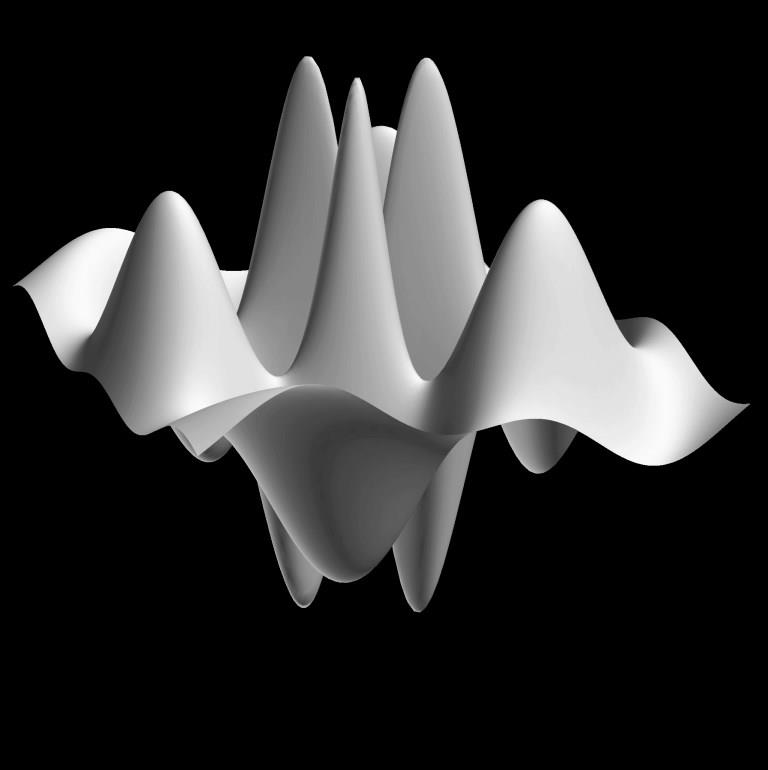
\includegraphics[scale=3.0]{Charts/jpg/SurfaceBlackAndWhite.jpg}
	\caption{plot of a 2-dimensional function}
	\label{Fig plot of a 2-dimensional function}
\end{figure}


The corresponding code is:
\lstset{language={[Sharp]C}}
\begin{lstlisting}
const double two_pi = 2 * Math.PI;
double r2 = x * x + z * z;
double r = Math.Sqrt(r2);
double theta = Math.Atan2(z, x);
result = Math.Exp(-r2) * Math.Sin(two_pi * r) * Math.Cos(3 * theta);
\end{lstlisting}


\newpage
\subsection{Surface plots for bivariate real functions}
%\lipsum[2]

The bivariate normal distribution has the following density:
\begin{equation}
	g(x,y;\rho) = \frac{1}{2 \pi \sqrt{1-\rho^2}} e^{\frac{-(x^2 -2\rho x y + y^2)}{2(1-\rho^2)}}
\end{equation}


\begin{figure}[ht]
	\centering
	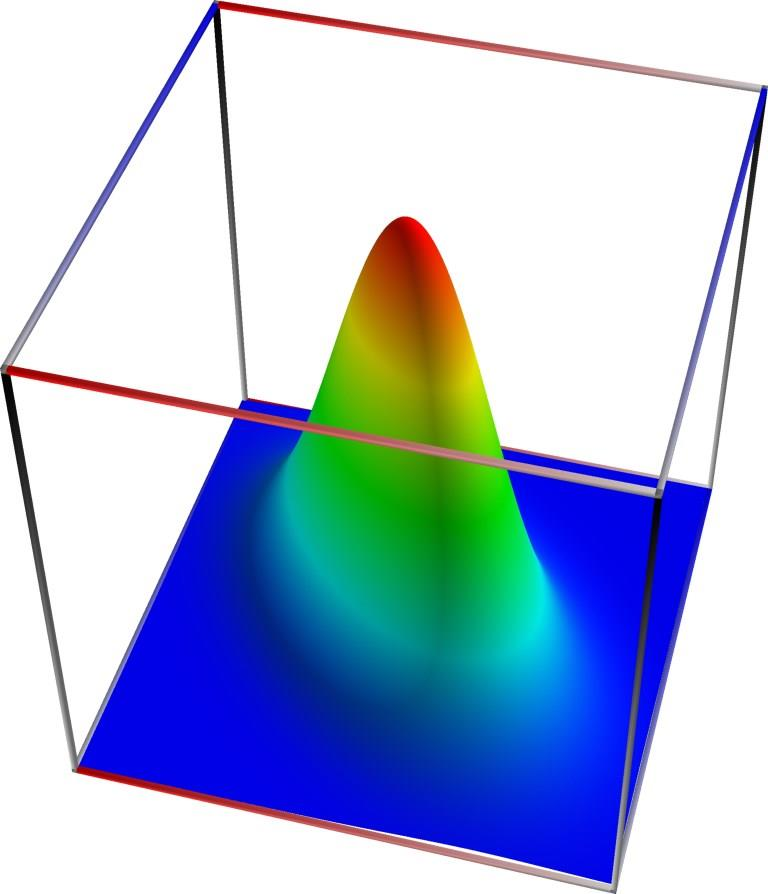
\includegraphics[scale=3.0]{Charts/jpg/BivariateNormal2.jpg}
	\caption{Surface plot of the probability density function of the bivariate normal distribution with $\rho = - 0.5$ }
	\label{Fig plot of the bivariate normal distribution}
\end{figure}


The corresponding code is:
\lstset{language={[Sharp]C}}
\begin{lstlisting}
const double two_pi = 2 * Math.PI;
double rho = -0.5;
double r2 = 1.0 - rho*rho;
double f = 1 / (two_pi * Math.Sqrt(r2));
double e = -(x*x - 2*rho*x*z + z*z)/(2*r2);
result = f * Math.Exp(e);
\end{lstlisting}


\newpage
\subsection{3D Plots of parametric functions}
%\lipsum[1]

\subsubsection{3D Plot of a Seashell}

This is a plot of a seashell. 

\begin{figure}[ht]
	\centering
	\includegraphics[scale=3.0]{Charts/jpg/Seashell.jpg}
	\caption[3D plot of a parametric function: Seashell]{3D plot of a parametric function: Seashell. umin = 0; umax = 6*Math.PI; umin = 0; umax = 6*Math.PI. Camera angles are $\theta = 135\degree$ and $\phi = -12\degree$.}
	\label{Fig 3D plot of a parametric function: Seashell}
\end{figure}


The parametrization is:
\lstset{language={[Sharp]C}}
\begin{lstlisting}
double a = Math.Exp(u / (6.0 * Math.PI));
double b = Math.Cos(v / 2.0);

x = 2.0 * (1.0 - a) * Math.Cos(u) * b * b;
z = 2.0 * (-1.0 + a) * Math.Sin(u) * b * b;
y = 1.0 - a * a - Math.Sin(v) * (1.0 - a);
\end{lstlisting}



\newpage
\subsubsection{3D Plot of Kuen's surface}

This is a plot of Kuen's surface. 

\begin{figure}[ht]
	\centering
	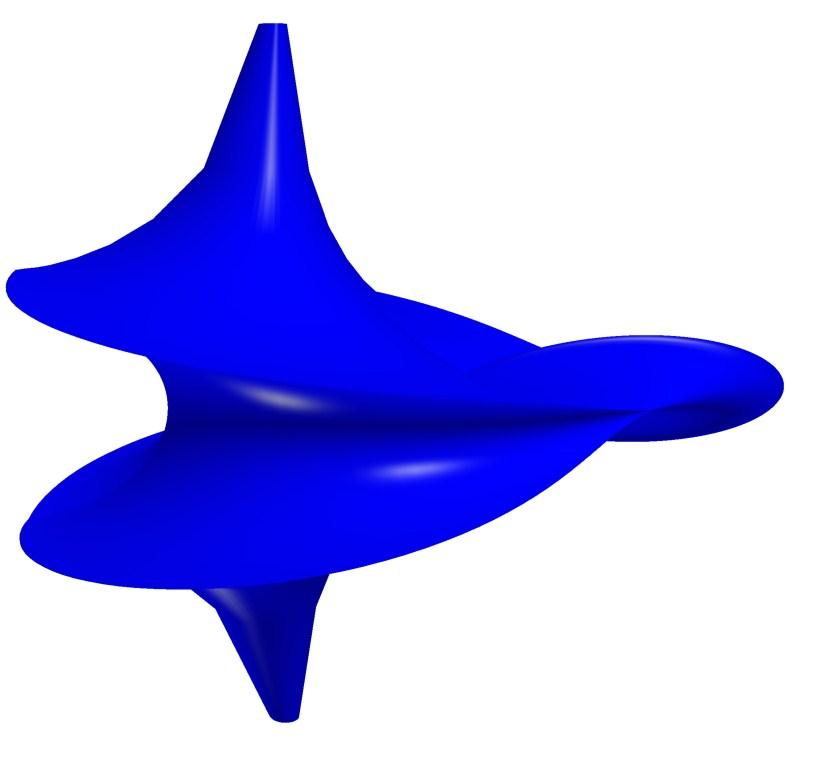
\includegraphics[scale=3.0]{Charts/jpg/KuenSurface.jpg}
	\caption[3D plot of Kuen's surface]{3D plot of a parametric function: Kuen's surface. umin = -4.5; umax = 4.5; vmin = 0.01; vmax = 3.14. Camera angles are $\theta = 135\degree$ and $\phi = -12\degree$.}
	\label{Fig 3D plot of a parametric function: Kuen's surface}
\end{figure}


The parametrization is:
\lstset{language={[Sharp]C}}
\begin{lstlisting}
double a = 1.0 * Math.Sin(v);
double b = 1.0 + u * u * a * a;

x = 2.0 * a * (Math.Cos(u) + u * Math.Sin(u)) / b;
z = 2.0 * a * (Math.Sin(u) - u * Math.Cos(u)) / b;
y = Math.Log(Math.Tan(v/2.0)) + 2.0 * Math.Cos(v) / b;
\end{lstlisting}



\newpage
\subsubsection{3D Plot of Klein's Bottle}

This is a plot of Klein's Bottle. 

\begin{figure}[ht]
	\centering
	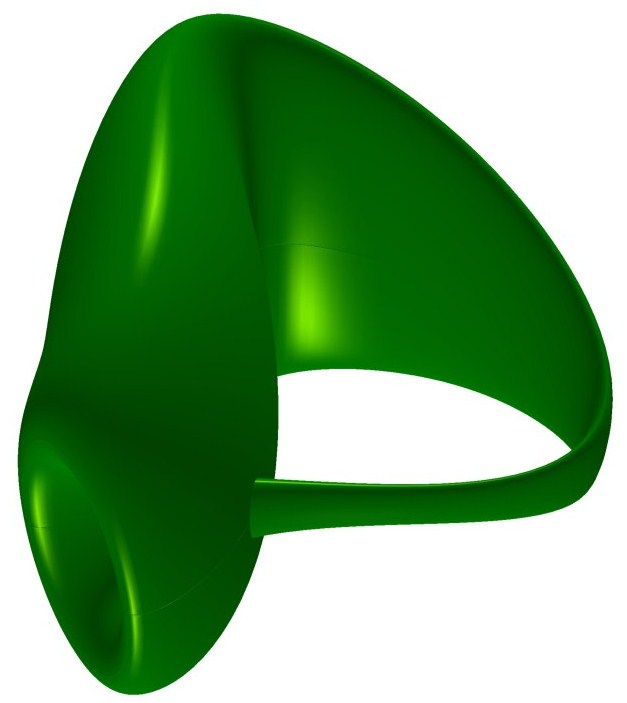
\includegraphics[scale=3.0]{Charts/jpg/KleinBottle.jpg}
	\caption[3D plot of Klein's Bottle]{3D plot of a parametric function: Klein's Bottle. umin = 0.0; umax = 3.14; vmin = 0.0; vmax = 6.28. Camera angles are $\theta = 135\degree$ and $\phi = -12\degree$.}
	\label{Fig 3D plot of a parametric function: Klein's Bottle}
\end{figure}


The following parametrization is due to Robert Israel (with some rearrangements):
\lstset{language={[Sharp]C}}
\begin{lstlisting}
double a = Math.Cos(u);
double b = Math.Sin(u);
double c = Math.Cos(v);
double a2 = a * a;
double a4 = a2 * a2;

x = -(2.0/15.0) * a * (3*c + b*(-30 + a4*(90 - 60*a2) + 5*a*c));
z = -(1.0/15.0) * b*b * (c*b* (3 - 48*a4  + 5*a*b*(1 - 16*a4)) - 60);
y = (2.0/15.0) * (3 + 5*a*b) * Math.Sin(v);
\end{lstlisting}





\newpage
\subsection{Surface plots of complex functions}
\label{Graphics: Surface plots of complex functions}
It is straight forward to produce surface plots of complex functions; these are available in two forms:

\vpara
As plots of the real and imaginary component:

\begin{figure}[ht]
	\centering
	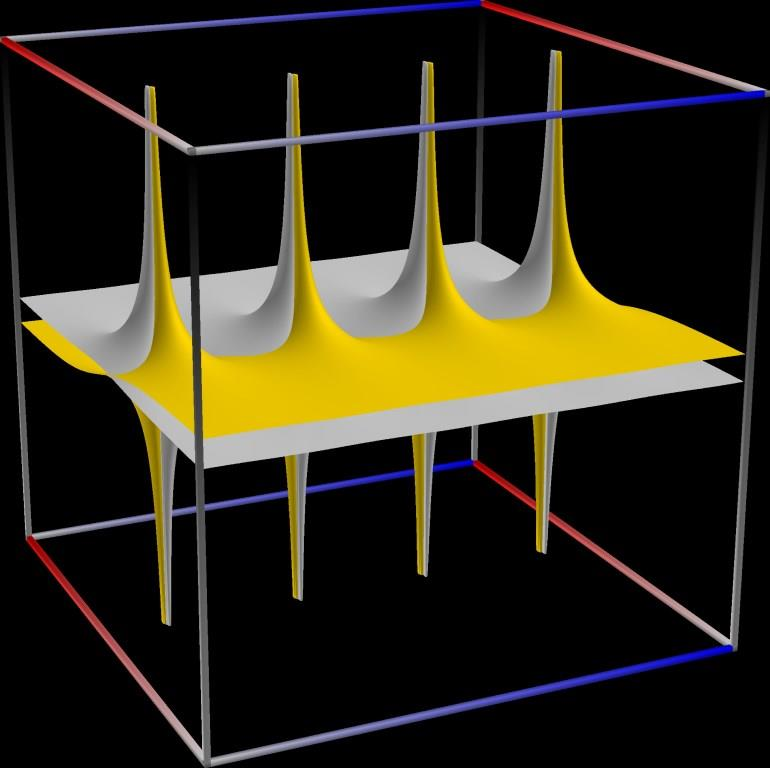
\includegraphics[scale=3.0]{Charts/jpg/ComplexSurfacePlotRealAndImaginary.jpg}
	\caption[Surface plot of the real and imaginary component of $z = \tan(x + iy)$]{Surface plot of the real ("silver") and imaginary ("gold") component of $z = \tan(x + iy)$, $-3 \leq x \leq 3$ (blue axis), $-2 \pi \leq y \leq 2\pi$ (red axis), $-10 \leq z \leq 10$ (black axis). $z$ values are truncated at $\pm 10$. There is a branch cut along the negative real axis. Camera angles are $\theta = 135\degree$ and $\phi = -12\degree$.}
	\label{Fig plot of the re and im of complex tangent}
\end{figure}



%\subsection{Pretty Formatting (specify extra digits)}

\newpage
%\subsection{File Output}
As plots of the absolute value with the phase color-coded:


\begin{figure}[ht]
	\centering
	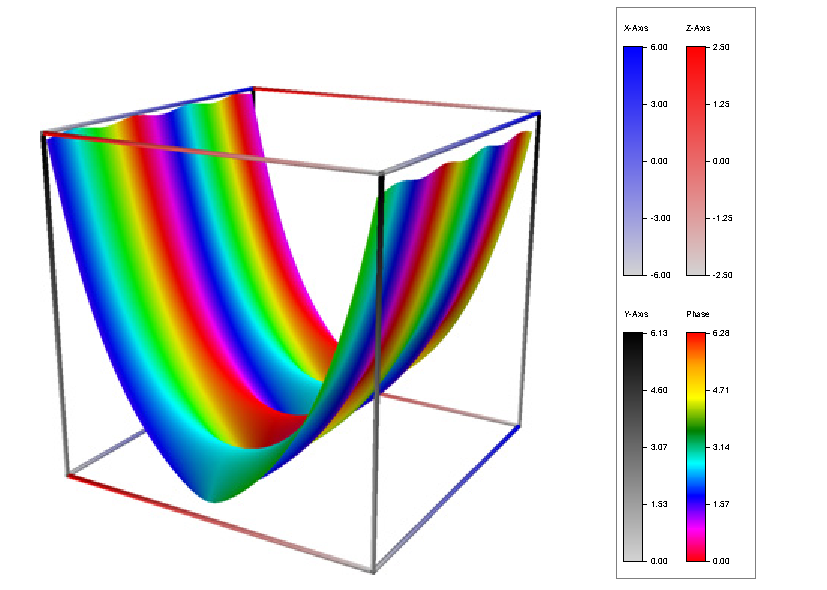
\includegraphics[scale=1.2]{Charts/pdf/SurfacePlotWithScales.pdf}
	\caption[Surface plot of the magnitude of $z = \sin(x + iy)$]{Surface plot of the magnitude and phase (color-coded) of $z = \sin(x + iy)$, $-3 \leq x \leq 3$ (blue axis), $-2 \pi \leq y \leq 2\pi$ (red axis), $-10 \leq z \leq 10$ (black axis). $z$ values are truncated at $\pm 10$. There is a branch cut along the negative real axis. Camera angles are $\theta = 135\degree$ and $\phi = -12\degree$. } 
	\label{Fig plot of the magnitude of complex sine}
\end{figure}






\newpage
\section{Eval, Options, Tables and Charts}

The following functions provide quick access to function evaluations and charts:

\vspace{0.3cm}
\begin{mpFunctionsExtract}
	\mpFunctionOne
	{Eval? String?  the result of the evaluation of an arithmetic expression, containing number and functions, but no variables.}
	{Expression? String? an arithmetic expression.}
\end{mpFunctionsExtract}


\vspace{0.3cm}
\begin{mpFunctionsExtract}
	\mpFunctionOne
	{Options? String?  an identifier for a set of calculation options.}
	{BaseOptions? String? an identifier for a set of base calculation options.}
\end{mpFunctionsExtract}


\vspace{0.3cm}
\begin{mpFunctionsExtract}
	\mpFunctionOne
	{Table? Range?  an identifier for a set of calculation options.}
	{TableRef? String? a reference for a table.}
\end{mpFunctionsExtract}


\vspace{0.3cm}
\begin{mpFunctionsExtract}
	\mpFunctionOne
	{Chart? String?  an identifier for an XML Chart.}
	{Data? Range? a reference for a data table.}
\end{mpFunctionsExtract}





\part{Functions with Error Bounds}
\chapter{Basic Usage}





In interactive code examples that follow, it will be assumed that all items in the mpFormulaPy
namespace have been imported:

\lstset{language={Python}}
\begin{lstlisting}
>>> from mpFormulaPy import *
\end{lstlisting}

Importing everything can be convenient, especially when using mpFormulaPy interactively, but be careful when mixing mpFormulaPy with other libraries! To avoid inadvertently overriding other functions or objects, explicitly import only the needed objects, or use the mpFormulaPy. or mp.namespaces:


\lstset{language={Python}}
\begin{lstlisting}
from mpFormulaPy import sin, cos
sin(1), cos(1)
import mpFormulaPy
mpFormulaPy.sin(1), mpFormulaPy.cos(1)
from mpFormulaPy import mp # mp context object -- to be explained
mp.sin(1), mp.cos(1)>>> from mpFormulaPy import *
\end{lstlisting}



\section{Number types}
Mpmath provides the following numerical types:

\begin{verbatim}
Class Description
mpf Real float
mpc Complex float
matrix Matrix
\end{verbatim}


Currently missing: decimals. The MPD reference is \cite{mpd_2012}


The following section will provide a very short introduction to the types mpf and mpc. Intervals and matrices are described further in the documentation chapters on interval arithmetic and matrices / linear algebra.

\vpara
The mpf type is analogous to Python's built-in float. It holds a real number or one of the special values inf (positive infinity), -inf (negative infinity) and nan (not-a-number, indicating an indeterminate result). You can create mpf instances from strings, integers, floats, and
other mpf instances:

\lstset{language={Python}}
\begin{lstlisting}
>>> mpf(4)
mpf('4.0')
>>> mpf(2.5)
mpf('2.5')
>>> mpf("1.25e6")
mpf('1250000.0')
>>> mpf(mpf(2))
mpf('2.0')
>>> mpf("inf")
mpf('+inf')
\end{lstlisting}


The mpc type represents a complex number in rectangular form as a pair of mpf instances. It can be constructed from a Python complex, a real number, or a pair of real numbers:

\lstset{language={Python}}
\begin{lstlisting}
>>> mpc(2,3)
mpc(real='2.0', imag='3.0')
>>> mpc(complex(2,3)).imag
mpf('3.0')
\end{lstlisting}


You can mix mpf and mpc instances with each other and with Python numbers:

\lstset{language={Python}}
\begin{lstlisting}
>>> mpf(3) + 2*mpf('2.5') + 1.0
mpf('9.0')
>>> mp.dps = 15 # Set precision (see below)
>>> mpc(1j)**0.5
mpc(real='0.70710678118654757', imag='0.70710678118654757')
\end{lstlisting}


\subsection{Setting the precision} 

Mpmath uses a global working precision; it does not keep track of the precision or accuracy of individual numbers. Performing an arithmetic operation or calling mpf() rounds the result to the current working precision. The working precision is controlled by a context object called mp, which has the following default states:

\lstset{language={Python}}
\begin{lstlisting}
>>> from mpFormulaPy import *
>>> mp.dps
25
>>> mp.prec
86
>>> mp.trap_complex
False
>>>
\end{lstlisting}


The term prec denotes the binary precision (measured in bits) while dps (short for decimal places) is the decimal precision. Binary and decimal precision are related roughly according to the formula prec = 3.33*dps. For example, it takes a precision of roughly 333 bits to hold an approximation of pi that is accurate to 100 decimal places (actually slightly more than 333 bits is used).

\vpara
Changing either precision property of the mp object automatically updates the other; usually you just want to change the dps value:

\lstset{language={Python}}
\begin{lstlisting}
>>> mp.dps = 100
>>> mp.dps
100
>>> mp.prec
336
\end{lstlisting}


When the precision has been set, all mpf operations are carried out at that precision:

\lstset{language={Python}}
\begin{lstlisting}
>>> mp.dps = 50
>>> mpf(1) / 6
mpf('0.16666666666666666666666666666666666666666666666666656')
>>> mp.dps = 25
>>> mpf(2) ** mpf('0.5')
mpf('1.414213562373095048801688713')
\end{lstlisting}

The precision of complex arithmetic is also controlled by the mp object:

\lstset{language={Python}}
\begin{lstlisting}
>>> mp.dps = 10
>>> mpc(1,2) / 3
mpc(real='0.3333333333321', imag='0.6666666666642')
\end{lstlisting}


There is no restriction on the magnitude of numbers. An mpf can for example hold an approximation of a large Mersenne prime:

\lstset{language={Python}}
\begin{lstlisting}
>>> mp.dps = 15
>>> print mpf(2)**32582657 - 1
1.24575026015369e+9808357
\end{lstlisting}


Or why not 1 googolplex:

\lstset{language={Python}}
\begin{lstlisting}
>>> print mpf(10) ** (10**100)
1.0e+100000000000000000000000000000000000000000000000000...
\end{lstlisting}


The (binary) exponent is stored exactly and is independent of the precision.


\subsection{Temporarily changing the precision}  

It is often useful to change the precision during only part of a calculation. A way to temporarily increase the precision and then restore it is as follows:

\lstset{language={Python}}
\begin{lstlisting}
>>> mp.prec += 2
>>> # do_something()
>>> mp.prec -= 2
\end{lstlisting}


As of Python 2.5, the with statement along with the mpFormulaPy functions workprec, workdps, extraprec and extradps can be used to temporarily change precision in a more safe manner:

\lstset{language={Python}}
\begin{lstlisting}
>>> from __future__ import with_statement
>>> with workdps(20):
... print mpf(1)/7
... with extradps(10):
... print mpf(1)/7
...
0.14285714285714285714
0.142857142857142857142857142857
>>> mp.dps
15
\end{lstlisting}


The with statement ensures that the precision gets reset when exiting the block, even in the case that an exception is raised. (The effect of the with statement can be emulated in Python 2.4 by using a try/finally block.)

The workprec family of functions can also be used as function decorators:

\lstset{language={Python}}
\begin{lstlisting}
>>> @workdps(6)
... def f():
... return mpf(1)/3
...
>>> f()
mpf('0.33333331346511841')
\end{lstlisting}


Some functions accept the prec and dps keyword arguments and this will override the global working precision. Note that this will not affect the precision at which the result is printed, so to get all digits, you must either use increase precision afterward when printing or use nstr/nprint:

\lstset{language={Python}}
\begin{lstlisting}
>>> mp.dps = 15
>>> print exp(1)
2.71828182845905
>>> print exp(1, dps=50) # Extra digits won't be printed
2.71828182845905
>>> nprint(exp(1, dps=50), 50)
2.7182818284590452353602874713526624977572470937
\end{lstlisting}


Finally, instead of using the global context object mp, you can create custom contexts and work with methods of those instances instead of global functions. The working precision will be local to each context object:

\lstset{language={Python}}
\begin{lstlisting}
>>> mp2 = mp.clone()
>>> mp.dps = 10
>>> mp2.dps = 20
>>> print mp.mpf(1) / 3
0.3333333333
>>> print mp2.mpf(1) / 3
0.33333333333333333333
\end{lstlisting}


Note: the ability to create multiple contexts is a new feature that is only partially implemented. Not all mpFormulaPy functions are yet available as context-local methods. In the present version, you are likely to encounter bugs if you try mixing different contexts.


\subsection{Providing correct input}  

Note that when creating a new mpf, the value will at most be as accurate as the input. Be careful when mixing mpFormulaPy numbers with Python floats. When working at high precision, fractional mpf values should be created from strings or integers:

\lstset{language={Python}}
\begin{lstlisting}
>>> mp.dps = 30
>>> mpf(10.9) # bad
mpf('10.9000000000000003552713678800501')
>>> mpf('10.9') # good
mpf('10.8999999999999999999999999999997')
>>> mpf(109) / mpf(10) # also good
mpf('10.8999999999999999999999999999997')
>>> mp.dps = 15
\end{lstlisting}


(Binary fractions such as 0.5, 1.5, 0.75, 0.125, etc, are generally safe as input, however, since those can be represented exactly by Python floats.)


\subsection{Printing}  

By default, the repr() of a number includes its type signature. This way eval can be used to recreate a number from its string representation:

\lstset{language={Python}}
\begin{lstlisting}
>>> eval(repr(mpf(2.5)))
mpf('2.5')
\end{lstlisting}


Prettier output can be obtained by using str() or print, which hide the mpf and mpc signatures and also suppress rounding artifacts in the last few digits:

\lstset{language={Python}}
\begin{lstlisting}
>>> mpf("3.14159")
mpf('3.1415899999999999')
>>> print mpf("3.14159")
3.14159
>>> print mpc(1j)**0.5
(0.707106781186548 + 0.707106781186548j)
\end{lstlisting}


Setting the mp.pretty option will use the str()-style output for repr() as well:

\lstset{language={Python}}
\begin{lstlisting}
>>> mp.pretty = True
>>> mpf(0.6)
0.6
>>> mp.pretty = False
>>> mpf(0.6)
mpf('0.59999999999999998')
\end{lstlisting}


The number of digits with which numbers are printed by default is determined by the working precision. To specify the number of digits to show without changing the working precision, use mpFormulaPy.nstr() and mpFormulaPy.nprint():

\lstset{language={Python}}
\begin{lstlisting}
>>> a = mpf(1) / 6
>>> a
mpf('0.16666666666666666')
>>> nstr(a, 8)
'0.16666667'
>>> nprint(a, 8)
0.16666667
>>> nstr(a, 50)
'0.16666666666666665741480812812369549646973609924316'
\end{lstlisting}














\subsection{Contexts}  

High-level code in mpFormulaPy is implemented as methods on a 'context object'. The context implements arithmetic, type conversions and other fundamental operations. The context also holds settings such as precision, and stores cache data. A few different contexts (with a
mostly compatible interface) are provided so that the high-level algorithms can be used with different implementations of the underlying arithmetic, allowing different features and speed/accuracy tradeoffs. Currently, mpFormulaPy provides the following contexts:

\vpara
Arbitrary-precision arithmetic (mp)

A faster Cython-based version of mp (used by default in Sage, and currently only available there)

Arbitrary-precision interval arithmetic (iv)

Double-precision arithmetic using Python's builtin float and complex types (fp)

\vpara
Most global functions in the global mpFormulaPy namespace are actually methods of the mp context. This fact is usually transparent to the user, but sometimes shows up in the form of an initial parameter called 'ctx' visible in the help for the function:

\lstset{language={Python}}
\begin{lstlisting}
>>> import mpFormulaPy
>>> help(mpFormulaPy.fsum)
Help on method fsum in module mpFormulaPy.ctx_mp_python:
fsum(ctx, terms, absolute=False, squared=False) method of mpFormulaPy.ctx_mp.MPContext ins
Calculates a sum containing a finite number of terms (for infinite
series, see :func:`~mpFormulaPy.nsum`). The terms will be converted to
...
\end{lstlisting}



The following operations are equivalent:

\lstset{language={Python}}
\begin{lstlisting}
>>> mpFormulaPy.mp.dps = 15; mpFormulaPy.mp.pretty = False
>>> mpFormulaPy.fsum([1,2,3])
mpf('6.0')
>>> mpFormulaPy.mp.fsum([1,2,3])
mpf('6.0')
\end{lstlisting}


The corresponding operation using the fp context:

\lstset{language={Python}}
\begin{lstlisting}
>>> mpFormulaPy.fp.fsum([1,2,3])
6.0
\end{lstlisting}


\subsection{Common interface}  

ctx.mpf creates a real number:

\lstset{language={Python}}
\begin{lstlisting}
>>> from mpFormulaPy import mp, fp
>>> mp.mpf(3)
mpf('3.0')
>>> fp.mpf(3)
3.0
\end{lstlisting}


ctx.mpc creates a complex number:

\lstset{language={Python}}
\begin{lstlisting}
>>> mp.mpc(2,3)
mpc(real='2.0', imag='3.0')
>>> fp.mpc(2,3)
(2+3j)
\end{lstlisting}


ctx.matrix creates a matrix:

\lstset{language={Python}}
\begin{lstlisting}
>>> mp.matrix([[1,0],[0,1]])
matrix(
[['1.0', '0.0'],
['0.0', '1.0']])
>>> _[0,0]
mpf('1.0')
>>> fp.matrix([[1,0],[0,1]])
matrix(
[['1.0', '0.0'],
['0.0', '1.0']])
>>> _[0,0]
1.0
\end{lstlisting}


ctx.prec holds the current precision (in bits):

\lstset{language={Python}}
\begin{lstlisting}
>>> mp.prec
53
>>> fp.prec
53
\end{lstlisting}


ctx.dps holds the current precision (in digits):

\lstset{language={Python}}
\begin{lstlisting}
>>> mp.dps
15
>>> fp.dps
15
\end{lstlisting}


ctx.pretty controls whether objects should be pretty-printed automatically by repr(). Prettyprinting for mp numbers is disabled by default so that they can clearly be distinguished from Python numbers and so that eval(repr(x)) == x works:

\lstset{language={Python}}
\begin{lstlisting}
>>> mp.mpf(3)
mpf('3.0')
>>> mpf = mp.mpf
>>> eval(repr(mp.mpf(3)))
mpf('3.0')
>>> mp.pretty = True
>>> mp.mpf(3)
3.0
>>> fp.matrix([[1,0],[0,1]])
matrix(
[['1.0', '0.0'],
['0.0', '1.0']])
>>> fp.pretty = True
>>> fp.matrix([[1,0],[0,1]])
[1.0 0.0]
[0.0 1.0]
>>> fp.pretty = False
>>> mp.pretty = False
\end{lstlisting}



\subsection{Arbitrary-precision floating-point (mp)}  

The mp context is what most users probably want to use most of the time, as it supports the most functions, is most well-tested, and is implemented with a high level of optimization. Nearly all examples in this documentation use mp functions.

See Basic usage for a description of basic usage.


\subsection{Arbitrary-precision interval arithmetic (iv)}  

The iv.mpf type represents a closed interval $[a,]$; that is, the set $\{x: a \leq x \leq b\}$, where $a$ and $b $ are arbitrary-precision floating-point values, possibly $\pm\infty$. The iv.mpc type represents a rectangular complex interval $[a,b] + [c,d]i$; that is, the set $\{z=x+iy: a \leq x \leq b \wedge c \leq y \leq d\}$.

\vpara
Interval arithmetic provides rigorous error tracking. If  $f$ is a mathematical function and $\hat{f}$ is its interval arithmetic version, then the basic guarantee of interval arithmetic is that $f(v) \subseteq \hat{f}(v)$ for any input interval $v$. Put differently, if an interval represents the known uncertainty for a fixed number, any sequence of interval operations will produce an interval that contains what would be the result of applying the same sequence of operations to the exact number. The principal drawbacks of interval arithmetic are speed (iv arithmetic is typically at least two times slower than mp arithmetic) and that it sometimes provides far too pessimistic bounds.

\vpara
Note: The support for interval arithmetic in mpFormulaPy is still experimental, and many functions do not yet properly support intervals. Please use this feature with caution.

\vpara
Intervals can be created from single numbers (treated as zero-width intervals) or pairs of endpoint numbers. Strings are treated as exact decimal numbers. Note that a Python float like 0.1 generally does not represent the same number as its literal; use '0.1' instead:

\lstset{language={Python}}
\begin{lstlisting}
>>> from mpFormulaPy import iv
>>> iv.dps = 15; iv.pretty = False
>>> iv.mpf(3)
mpi('3.0', '3.0')
>>> print iv.mpf(3)
[3.0, 3.0]
>>> iv.pretty = True
>>> iv.mpf([2,3])
[2.0, 3.0]
>>> iv.mpf(0.1) # probably not intended
[0.10000000000000000555, 0.10000000000000000555]
>>> iv.mpf('0.1') # good, gives a containing interval
[0.099999999999999991673, 0.10000000000000000555]
>>> iv.mpf(['0.1', '0.2'])
[0.099999999999999991673, 0.2000000000000000111]
\end{lstlisting}


The fact that '0.1' results in an interval of nonzero width indicates that 1/10 cannot be represented using binary floating-point numbers at this precision level (in fact, it cannot be represented exactly at any precision).

\vpara
Intervals may be infinite or half-infinite:

\lstset{language={Python}}
\begin{lstlisting}
>>> print 1 / iv.mpf([2, 'inf'])
[0.0, 0.5]
\end{lstlisting}


The equality testing operators $==$ and $!=$ check whether their operands are identical as intervals; that is, have the same endpoints. The ordering operators $<$,  $<=$,  $>$ and $>=$ permit inequality testing using triple-valued logic: a guaranteed inequality returns True or False while an indeterminate inequality returns None:

\lstset{language={Python}}
\begin{lstlisting}
>>> iv.mpf([1,2]) == iv.mpf([1,2])
True
>>> iv.mpf([1,2]) != iv.mpf([1,2])
False
>>> iv.mpf([1,2]) <= 2
True
>>> iv.mpf([1,2]) > 0
True
>>> iv.mpf([1,2]) < 1
False
>>> iv.mpf([1,2]) < 2 # returns None
>>> iv.mpf([2,2]) < 2
False
>>> iv.mpf([1,2]) <= iv.mpf([2,3])
True
>>> iv.mpf([1,2]) < iv.mpf([2,3]) # returns None
>>> iv.mpf([1,2]) < iv.mpf([-1,0])
False
\end{lstlisting}


The in operator tests whether a number or interval is contained in another interval:

\lstset{language={Python}}
\begin{lstlisting}
>>> iv.mpf([0,2]) in iv.mpf([0,10])
True
>>> 3 in iv.mpf(['-inf', 0])
False
\end{lstlisting}


Intervals have the properties .a, .b (endpoints), .mid, and .delta (width):

\lstset{language={Python}}
\begin{lstlisting}
>>> x = iv.mpf([2, 5])
>>> x.a
[2.0, 2.0]
>>> x.b
[5.0, 5.0]
>>> x.mid
[3.5, 3.5]
>>> x.delta
[3.0, 3.0]
\end{lstlisting}


Some transcendental functions are supported:

\lstset{language={Python}}
\begin{lstlisting}
>>> iv.dps = 15
>>> mp.dps = 15
>>> iv.mpf([0.5,1.5]) ** iv.mpf([0.5, 1.5])
[0.35355339059327373086, 1.837117307087383633]
>>> iv.exp(0)
[1.0, 1.0]
>>> iv.exp(['-inf','inf'])
[0.0, +inf]
>>>
>>> iv.exp(['-inf',0])
[0.0, 1.0]
>>> iv.exp([0,'inf'])
[1.0, +inf]
>>> iv.exp([0,1])
[1.0, 2.7182818284590455349]
>>>
>>> iv.log(1)
[0.0, 0.0]
>>> iv.log([0,1])
[-inf, 0.0]
>>> iv.log([0,'inf'])
[-inf, +inf]
>>> iv.log(2)
[0.69314718055994528623, 0.69314718055994539725]
>>>
>>> iv.sin([100,'inf'])
[-1.0, 1.0]
>>> iv.cos(['-0.1','0.1'])
[0.99500416527802570954, 1.0]
\end{lstlisting}


Interval arithmetic is useful for proving inequalities involving irrational numbers. Naive use of mp arithmetic may result in wrong conclusions, such as the following:

\lstset{language={Python}}
\begin{lstlisting}
>>> mp.dps = 25
>>> x = mp.exp(mp.pi*mp.sqrt(163))
>>> y = mp.mpf(640320**3+744)
>>> print x
262537412640768744.0000001
>>> print y
262537412640768744.0
>>> x > y
True
\end{lstlisting}


But the correct result is $e^{\pi\sqrt{163}} < 262537412640768744$, as can be seen by increasing the precision:

\lstset{language={Python}}
\begin{lstlisting}
>>> mp.dps = 50
>>> print mp.exp(mp.pi*mp.sqrt(163))
262537412640768743.99999999999925007259719818568888
\end{lstlisting}


With interval arithmetic, the comparison returns None until the precision is large enough for $x-y$ to have a definite sign:

\lstset{language={Python}}
\begin{lstlisting}
>>> iv.dps = 15
>>> iv.exp(iv.pi*iv.sqrt(163)) > (640320**3+744)
>>> iv.dps = 30
>>> iv.exp(iv.pi*iv.sqrt(163)) > (640320**3+744)
>>> iv.dps = 60
>>> iv.exp(iv.pi*iv.sqrt(163)) > (640320**3+744)
False
>>> iv.dps = 15
\end{lstlisting}


\subsection{Fast low-precision arithmetic (fp)}  

Although mpFormulaPy is generally designed for arbitrary-precision arithmetic, many of the high-level algorithms work perfectly well with ordinary Python float and complex numbers, which use hardware double precision (on most systems, this corresponds to 53 bits of precision). 

Whereas the global functions (which are methods of the mp object) always
convert inputs to mpFormulaPy numbers, the fp object instead converts them to float or complex, and in some cases employs basic functions optimized for double precision. When large amounts of function evaluations (numerical integration, plotting, etc) are required, and when
fp arithmetic provides sufficient accuracy, this can give a significant speedup over mp arithmetic.

\vpara
To take advantage of this feature, simply use the fp prefix, i.e. write fp.func instead of func or mp.func:

\lstset{language={Python}}
\begin{lstlisting}
>>> u = fp.erfc(2.5)
>>> print u
0.000406952017445
>>> type(u)
<type 'float'>
>>> mp.dps = 15
>>> print mp.erfc(2.5)
0.000406952017444959
>>> fp.matrix([[1,2],[3,4]]) ** 2
matrix(
[['7.0', '10.0'],
['15.0', '22.0']])
>>>
>>> type(_[0,0])
<type 'float'>
>>> print fp.quad(fp.sin, [0, fp.pi]) # numerical integration
2.0
\end{lstlisting}


The fp context wraps Python's math and cmath modules for elementary functions. It supports both real and complex numbers and automatically generates complex results for real inputs (math raises an exception):

\lstset{language={Python}}
\begin{lstlisting}
>>> fp.sqrt(5)
2.23606797749979
>>> fp.sqrt(-5)
2.23606797749979j
>>> fp.sin(10)
-0.5440211108893698
>>> fp.power(-1, 0.25)
(0.7071067811865476+0.7071067811865475j)
>>> (-1) ** 0.25
Traceback (most recent call last):
...
ValueError: negative number cannot be raised to a fractional power
\end{lstlisting}


The prec and dps attributes can be changed (for interface compatibility with the mp context) but this has no effect:

\lstset{language={Python}}
\begin{lstlisting}
>>> fp.prec
53
>>> fp.dps
15
>>> fp.prec = 80
>>> fp.prec
53
>>> fp.dps
15
\end{lstlisting}


Due to intermediate rounding and cancellation errors, results computed with fp arithmetic may be much less accurate than those computed with mp using an equivalent precision (mp.prec = 53), since the latter often uses increased internal precision. The accuracy is highly problem-dependent: for some functions, fp almost always gives 14-15 correct digits; for others, results can be accurate to only 2-3 digits or even completely wrong. The recommended use for fp is therefore to speed up large-scale computations where accuracy can be verified in advance on a subset of the input set, or where results can be verified afterwards.




\newpage
\section{Precision and representation issues}

Most of the time, using mpFormulaPy is simply a matter of setting the desired precision and entering a formula. For verification purposes, a quite (but not always!) reliable technique is to calculate the same thing a second time at a higher precision and verifying that the results
agree.

\vpara
To perform more advanced calculations, it is important to have some understanding of how mpFormulaPy works internally and what the possible sources of error are. This section gives an overview of arbitrary-precision binary floating-point arithmetic and some concepts from
numerical analysis.

\vpara
The following concepts are important to understand:

\vpara
The main sources of numerical errors are rounding and cancellation, which are due to the use of finite-precision arithmetic, and truncation or approximation errors, which are due to approximating infinite sequences or continuous functions by a finite number of samples.

\vpara
Errors propagate between calculations. A small error in the input may result in a large error in the output.

\vpara
Most numerical algorithms for complex problems (e.g. integrals, derivatives) give wrong answers for sufficiently ill-behaved input. Sometimes virtually the only way to get a wrong answer is to design some very contrived input, but at other times the chance of accidentally obtaining a wrong result even for reasonable-looking input is quite high.

\vpara
Like any complex numerical software, mpFormulaPy has implementation bugs. You should be reasonably suspicious about any results computed by mpFormulaPy, even those it claims to be able to compute correctly! If possible, verify results analytically, try different algorithms, and cross-compare with other software.



\subsection{Precision, error and tolerance}

The following terms are common in this documentation:

\vpara
Precision (or working precision) is the precision at which floating-point arithmetic operations are performed.

\vpara
Error is the difference between a computed approximation and the exact result.

\vpara
Accuracy is the inverse of error.

\vpara
Tolerance is the maximum error (or minimum accuracy) desired in a result.

\vpara
Error and accuracy can be measured either directly, or logarithmically in bits or digits. Specifically, if a $\hat{y}$ is an approximation for $y$, then

\vpara
(Direct) absolute error = $|\hat{y} - y|$

(Direct) relative error = $|\hat{y} - y||y|^{-1}$

(Direct) absolute accuracy = $|\hat{y} - y|^{-1}$

(Direct) relative accuracy = $|\hat{y} - y|^{-1}|y|$

(Logarithmic) absolute error = $\log_b|\hat{y} - y|$

(Logarithmic) relative error = $\log_b|\hat{y} - y| - \log_b|y|$

(Logarithmic) absolute accuracy = $-\log_b|\hat{y} - y|$

(Logarithmic) relative accuracy =$-\log_b|\hat{y} - y| - \log_b|y|$

\vpara
where $b=2$ and $b=10$ for bits and digits respectively. Note that:

\vpara
The logarithmic error roughly equals the position of the first incorrect bit or digit.

The logarithmic accuracy roughly equals the number of correct bits or digits in the result.

\vpara
These definitions also hold for complex numbers, using $|a+bi|=\sqrt{a^2+b^2}$.

Full accuracy means that the accuracy of a result at least equals prec-1, i.e. it is correct except possibly for the last bit.




\subsection{Representation of numbers}

Mpmath uses binary arithmetic. A binary floating-point number is a number of the form $man \times 2^{exp}$ where both man (the mantissa) and exp (the exponent) are integers. Some examples of floating-point numbers are given in the following table.

\vpara
\begin{verbatim}
Number Mantissa Exponent
3 3 0
10 5 1
-16 -1 4
1.25 5 -2
\end{verbatim}


\vpara
The representation as defined so far is not unique; one can always multiply the mantissa by 2 and subtract 1 from the exponent with no change in the numerical value. In mpFormulaPy, numbers are always normalized so that man is an odd number, with the exception of zero
which is always taken to have man = exp = 0. With these conventions, every representable number has a unique representation. (Mpmath does not currently distinguish between positive and negative zero.)

\vpara
Simple mathematical operations are now easy to define. Due to uniqueness, equality testing of two numbers simply amounts to separately checking equality of the mantissas and the exponents. Multiplication of nonzero numbers is straightforward: $(m2^e) \times (n2^f) = (mn) \times 2^{e+f}$. Addition is a bit more involved: we first need to multiply the mantissa of one of the operands by a suitable power of 2 to obtain equal exponents.

\vpara
More technically, mpFormulaPy represents a floating-point number as a 4-tuple (sign, man, exp, bc) where sign is 0 or 1 (indicating positive vs negative) and the mantissa is nonnegative; bc (bitcount) is the size of the absolute value of the mantissa as measured in bits. Though
redundant, keeping a separate sign field and explicitly keeping track of the bitcount significantly speeds up arithmetic (the bitcount, especially, is frequently needed but slow to compute from scratch due to the lack of a Python built-in function for the purpose).

\vpara
Contrary to popular belief, floating-point numbers do not come with an inherent 'small uncertainty', although floating-point arithmetic generally is inexact. Every binary floating-point number is an exact rational number. With arbitrary-precision integers used for the mantissa and exponent, floating-point numbers can be added, subtracted and multiplied exactly. In particular, integers and integer multiples of 1/2, 1/4, 1/8, 1/16, etc. can be represented, added and multiplied exactly in binary floating-point arithmetic.

\vpara
Floating-point arithmetic is generally approximate because the size of the mantissa must be limited for efficiency reasons. The maximum allowed width (bitcount) of the mantissa is called the precision or prec for short. Sums and products of floating-point numbers are exact
as long as the absolute value of the mantissa is smaller than $2^{prec}$. As soon as the mantissa becomes larger than this, it is truncated to contain at most prec bits (the exponent is incremented accordingly to preserve the magnitude of the number), and this operation introduces a rounding error. Division is also generally inexact; although we can add and
multiply exactly by setting the precision high enough, no precision is high enough to represent for example 1/3 exactly (the same obviously applies for roots, trigonometric functions, etc).

\vpara
The special numbers +inf, -inf and nan are represented internally by a zero mantissa and a nonzero exponent.

\vpara
Mpmath uses arbitrary precision integers for both the mantissa and the exponent, so numbers can be as large in magnitude as permitted by the computer's memory. Some care may be necessary when working with extremely large numbers. Although standard arithmetic operators are safe, it is for example futile to attempt to compute the exponential
function of of $10^{100000}$. Mpmath does not complain when asked to perform such a calculation, but instead chugs away on the problem to the best of its ability, assuming that computer resources are infinite. In the worst case, this will be slow and allocate a huge amount of memory; if entirely impossible Python will at some point raise OverflowError: long int too large to convert to int.

\vpara
For further details on how the arithmetic is implemented, refer to the mpFormulaPy source code. The basic arithmetic operations are found in the libmp directory; many functions there are commented extensively.






\subsection{Decimal issues}

Mpmath uses binary arithmetic internally, while most interaction with the user is done via the decimal number system. Translating between binary and decimal numbers is a somewhat subtle matter; many Python novices run into the following 'bug' (addressed in the General
Python FAQ):

\lstset{language={Python}}
\begin{lstlisting}
>>> 1.2 - 1.0
0.19999999999999996
\end{lstlisting}


Decimal fractions fall into the category of numbers that generally cannot be represented exactly in binary floating-point form. For example, none of the numbers 0.1, 0.01, 0.001 has an exact representation as a binary floating-point number. Although mpFormulaPy can
approximate decimal fractions with any accuracy, it does not solve this problem for all uses; users who need exact decimal fractions should look at the decimal module in Python's standard library (or perhaps use fractions, which are much faster).

\vpara
With prec bits of precision, an arbitrary number can be approximated relatively to within $2^{-prec}$, or within $10^{-dps}$ for dps decimal digits. The equivalent values for prec and dps are therefore related proportionally via the factor $C=\log(1)/\log(2)$, or roughly 3.32. For
example, the standard (binary) precision in mpFormulaPy is 53 bits, which corresponds to a decimal precision of 15.95 digits.

\vpara
More precisely, mpFormulaPy uses the following formulas to translate between prec and dps:

\lstset{language={Python}}
\begin{lstlisting}
dps(prec) = max(1, int(round(int(prec) / C - 1)))
prec(dps) = max(1, int(round((int(dps) + 1) * C)))
\end{lstlisting}

Note that the dps is set 1 decimal digit lower than the corresponding binary precision. This is done to hide minor rounding errors and artifacts resulting from binary-decimal conversion.
As a result, mpFormulaPy interprets 53 bits as giving 15 digits of decimal precision, not 16.

\vpara
The dps value controls the number of digits to display when printing numbers with str(),
while the decimal precision used by repr() is set two or three digits higher. For example,
with 15 dps we have:

\lstset{language={Python}}
\begin{lstlisting}
>>> from mpFormulaPy import *
>>> mp.dps = 15
>>> str(pi)
'3.14159265358979'
>>> repr(+pi)
"mpf('3.1415926535897931')"
\end{lstlisting}


The extra digits in the output from repr ensure that x == eval(repr(x)) holds, i.e. that numbers can be converted to strings and back losslessly.

\vpara
It should be noted that precision and accuracy do not always correlate when translating between binary and decimal. As a simple example, the number 0.1 has a decimal precision of 1 digit but is an infinitely accurate representation of 1/10. Conversely, the number $2^{-50}$ has a binary representation with 1 bit of precision that is infinitely accurate; the same number can actually be represented exactly as a decimal, but doing so requires 35 significant digits:

\lstset{language={Python}}
\begin{lstlisting}
0.00000000000000088817841970012523233890533447265625
\end{lstlisting}


All binary floating-point numbers can be represented exactly as decimals (possibly requiring many digits), but the converse is false.




\subsection{Correctness guarantees}

Basic arithmetic operations (with the mp context) are always performed with correct rounding. Results that can be represented exactly are guranteed to be exact, and results from single inexact operations are guaranteed to be the best possible rounded values. For higher-level
operations, mpFormulaPy does not generally guarantee correct rounding. In general, mpFormulaPy only guarantees that it will use at least the user-set precision to perform a given calculation. The user may have to manually set the working precision higher than the desired accuracy for the result, possibly much higher.

\vpara
Functions for evaluation of transcendental functions, linear algebra operations, numerical integration, etc., usually automatically increase the working precision and use a stricter tolerance to give a correctly rounded result with high probability: for example, at 50 bits the
temporary precision might be set to 70 bits and the tolerance might be set to 60 bits. It can often be assumed that such functions return values that have full accuracy, given inputs that are exact (or sufficiently precise approximations of exact values), but the user must exercise judgement about whether to trust mpFormulaPy.

\vpara
The level of rigor in mpFormulaPy covers the entire spectrum from 'always correct by design' through 'nearly always correct' and 'handling the most common errors' to 'just computing blindly and hoping for the best'. Of course, a long-term development goal is to successively
increase the rigor where possible. The following list might give an idea of the current state.

\vpara
Operations that are correctly rounded:

\vpara
Addition, subtraction and multiplication of real and complex numbers.
Division and square roots of real numbers.

Powers of real numbers, assuming sufficiently small integer exponents (huge powers are rounded in the right direction, but possibly farther than necessary).

Conversion from decimal to binary, for reasonably sized numbers (roughly $10^{-100}$ between and $10^{100}$).

Typically, transcendental functions for exact input-output pairs.

\vpara
Operations that should be fully accurate (however, the current implementation may be based on a heuristic error analysis):

\vpara
Radix conversion (large or small numbers).

Mathematical constants like $\pi$.

Both real and imaginary parts of exp, cos, sin, cosh, sinh, log.

Other elementary functions (the largest of the real and imaginary part).

The gamma and log-gamma functions (the largest of the real and the imaginary part; both, when close to real axis).

Some functions based on hypergeometric series (the largest of the real and imaginary part).

\vpara
Correctness of root-finding, numerical integration, etc. largely depends on the well-behavedness of the input functions. Specific limitations are sometimes noted in the respective sections of the documentation.



\subsection{Double precision emulation}

On most systems, Python's float type represents an IEEE 754 double precision number, with a precision of 53 bits and rounding-to-nearest. With default precision (mp.prec = 53), the mpFormulaPy mpf type roughly emulates the behavior of the float type. Sources of incompatibility
include the following:

In hardware floating-point arithmetic, the size of the exponent is restricted to a fixed range: regular Python floats have a range between roughly $10^{-300}$ and $10^{300}$). Mpmath does not emulate overflow or underflow when exponents fall outside this range.

On some systems, Python uses 80-bit (extended double) registers for floating-point operations. Due to double rounding, this makes the float type less accurate. This problem is only known to occur with Python versions compiled with GCC on 32-bit systems.

Machine floats very close to the exponent limit round subnormally, meaning that they lose accuracy (Python may raise an exception instead of rounding a float subnormally).

Mpmath is able to produce more accurate results for transcendental functions.





%\subsection{Quantize (only Decimal)}
%\begin{tabular}{p{481pt}}
%\toprule
%\textsf{Function \textbf{Quantize}($\boldsymbol{a}\ As\ mpNum$, $\boldsymbol{b}\ As\ mpNum$) As mpNum}\index{Multiprecision Functions!Quantize} \\
%\bottomrule
%\end{tabular}
%
%\vspace{0.3cm}
%\lipsum[2]
%


\newpage
\section{Conversion of formatted numbers}
\subsection{Conversions between Roman and Arabic Numbers}

\begin{mpFunctionsExtract}
	\mpWorksheetFunctionTwoNotImplemented
	{ROMAN? String? Converts an arabic numeral to roman, as text.}
	{Number? mpNum? The Arabic numeral you want converted.}
	{Form? Integer? A number from 0 to 4 specifying the type of roman numeral you want. The roman numeral style ranges from Classic to Simplified, becoming more concise as the value of form increases..}
\end{mpFunctionsExtract}

\vspace{0.6cm}

\begin{mpFunctionsExtract}
	\mpWorksheetFunctionOneNotImplemented
	{ARABIC? String? Converts an roman numeral to arabic, as text.}
	{Number? mpNum? The roman numeral you want converted.}
\end{mpFunctionsExtract}




\subsection{Conversions from Binary}

\begin{mpFunctionsExtract}
	\mpWorksheetFunctionOneNotImplemented
	{BIN2DEC? mpNum? Converts a binary number to decimal.}
	{Number? mpNum? The binary number you want to convert. Number cannot contain more than 10 characters (10 bits). The most significant bit of number is the sign bit. The remaining 9 bits are magnitude bits. Negative numbers are represented using two's-complement notation.}
\end{mpFunctionsExtract}


\vspace{0.6cm}
\begin{mpFunctionsExtract}
	\mpWorksheetFunctionTwoNotImplemented
	{BIN2HEX? mpNum? Converts a binary number to decimal.}
	{Number? mpNum? The binary number you want to convert. Number cannot contain more than 10 characters (10 bits). The most significant bit of number is the sign bit. The remaining 9 bits are magnitude bits. Negative numbers are represented using two's-complement notation.}
	{Places? mpNum? The number of characters to use. If places is omitted, BIN2HEX uses the minimum number of characters necessary. Places is useful for padding the return value with leading 0s (zeros).}
\end{mpFunctionsExtract}


\vspace{0.6cm}
\begin{mpFunctionsExtract}
	\mpWorksheetFunctionTwoNotImplemented
	{BIN2OCT? mpNum? Converts a binary number to octal.}
	{Number? mpNum? The binary number you want to convert. Number cannot contain more than 10 characters (10 bits). The most significant bit of number is the sign bit. The remaining 9 bits are magnitude bits. Negative numbers are represented using two's-complement notation.}
	{Places? mpNum? The number of characters to use. If places is omitted, BIN2OCT uses the minimum number of characters necessary. Places is useful for padding the return value with leading 0s (zeros).}
\end{mpFunctionsExtract}



\subsection{Conversions from Decimal}


\begin{mpFunctionsExtract}
	\mpWorksheetFunctionTwoNotImplemented
	{DEC2BIN? mpNum? Converts a decimal number to binary.}
	{Number? mpNum? The decimal integer you want to convert. If number is negative, valid place values are ignored and DEC2BIN returns a 10-character (10-bit) binary number in which the most significant bit is the sign bit. The remaining 9 bits are magnitude bits. Negative numbers are represented using two's-complement notation.}
	{Places? mpNum? The number of characters to use. If places is omitted, DEC2BIN uses the minimum number of characters necessary. Places is useful for padding the return value with leading 0s (zeros).}
\end{mpFunctionsExtract}


\vspace{0.6cm}
\begin{mpFunctionsExtract}
	\mpWorksheetFunctionTwoNotImplemented
	{DEC2HEX? mpNum? Converts a decimal number to hexadecimal.}
	{Number? mpNum? The decimal integer you want to convert. If number is negative, places is ignored and DEC2HEX returns a 10-character (40-bit) hexadecimal number in which the most significant bit is the sign bit. The remaining 39 bits are magnitude bits. Negative numbers are represented using two's-complement notation.}
	{Places? mpNum? The number of characters to use. If places is omitted, DEC2HEX uses the minimum number of characters necessary. Places is useful for padding the return value with leading 0s (zeros).}
\end{mpFunctionsExtract}


\vspace{0.6cm}
\begin{mpFunctionsExtract}
	\mpWorksheetFunctionTwoNotImplemented
	{DEC2OCT? mpNum? Converts a decimal number to octal.}
	{Number? mpNum? The decimal integer you want to convert. If number is negative, places is ignored and DEC2OCT returns a 10-character (30-bit) octal number in which the most significant bit is the sign bit. The remaining 29 bits are magnitude bits. Negative numbers are represented using two's-complement notation.}
	{Places? mpNum? The number of characters to use. If places is omitted, DEC2OCT uses the minimum number of characters necessary. Places is useful for padding the return value with leading 0s (zeros).}
\end{mpFunctionsExtract}




\subsection{Conversions from Hexadecimal}


\begin{mpFunctionsExtract}
	\mpWorksheetFunctionTwoNotImplemented
	{HEX2BIN? mpNum? Converts a  hexadecimal number to binary.}
	{Number? mpNum? The hexadecimal number you want to convert. Number cannot contain more than 10 characters. The most significant bit of number is the sign bit (40th bit from the right). The remaining 9 bits are magnitude bits. Negative numbers are represented using two's-complement notation.}
	{Places? mpNum? The number of characters to use. If places is omitted, HEX2BIN uses the minimum number of characters necessary. Places is useful for padding the return value with leading 0s (zeros).}
\end{mpFunctionsExtract}


\vspace{0.6cm}
\begin{mpFunctionsExtract}
	\mpWorksheetFunctionOneNotImplemented
	{HEX2DEC? mpNum? Converts a hexadecimal number to decimal.}
	{Number? mpNum? The hexadecimal number you want to convert. Number cannot contain more than 10 characters (40 bits). The most significant bit of number is the sign bit. The remaining 39 bits are magnitude bits. Negative numbers are represented using two's-complement notation}
\end{mpFunctionsExtract}


\vspace{0.6cm}
\begin{mpFunctionsExtract}
	\mpWorksheetFunctionTwoNotImplemented
	{HEX2OCT? mpNum? Converts a hexadecimal number to octal.}
	{Number? mpNum? The hexadecimal number you want to convert. Number cannot contain more than 10 characters. The most significant bit of number is the sign bit. The remaining 39 bits are magnitude bits. Negative numbers are represented using two's-complement notation.}
	{Places? mpNum? The number of characters to use. If places is omitted, HEX2OCT uses the minimum number of characters necessary. Places is useful for padding the return value with leading 0s (zeros).}
\end{mpFunctionsExtract}





\subsection{Conversions from Octal}

\begin{mpFunctionsExtract}
	\mpWorksheetFunctionTwoNotImplemented
	{OCT2BIN? mpNum? Converts a octal number to binary.}
	{Number? mpNum? The octal number you want to convert. Number may not contain more than 10 characters. The most significant bit of number is the sign bit. The remaining 29 bits are magnitude bits. Negative numbers are represented using two's-complement notation.}
	{Places? mpNum? The number of characters to use. If places is omitted, OCT2BIN uses the minimum number of characters necessary. Places is useful for padding the return value with leading 0s (zeros).}
\end{mpFunctionsExtract}


\vspace{0.6cm}
\begin{mpFunctionsExtract}
	\mpWorksheetFunctionOneNotImplemented
	{OCT2DEC? mpNum? Converts an octal number to decimal.}
	{Number? mpNum? The octal number you want to convert. Number may not contain more than 10 octal characters (30 bits). The most significant bit of number is the sign bit. The remaining 29 bits are magnitude bits. Negative numbers are represented using two's-complement notation.}
\end{mpFunctionsExtract}


\vspace{0.6cm}
\begin{mpFunctionsExtract}
	\mpWorksheetFunctionTwoNotImplemented
	{OCT2HEX? mpNum? Converts an octal number to hexadecimal.}
	{Number? mpNum? The octal number you want to convert. Number may not contain more than 10 octal characters (30 bits). The most significant bit of number is the sign bit. The remaining 29 bits are magnitude bits. Negative numbers are represented using two's-complement notation.}
	{Places? mpNum? The number of characters to use. If places is omitted, OCT2HEX uses the minimum number of characters necessary. Places is useful for padding the return value with leading 0s (zeros).}
\end{mpFunctionsExtract}



\subsection{Conversion to and from a Given Base}


\begin{mpFunctionsExtract}
	\mpWorksheetFunctionThree
	{BASE? mpNum? converts a number into a text representation with the given radix (base).}
	{Number? mpNum? The number that you want to convert. Must be an integer greater than or equal to 0 and less than $2^53$.}
	{Radix? mpNum? The base radix that you want to convert the number into. Must be an integer greater than or equal to 2 and less than or equal to 36.}
	{MinLength? mpNum? The minimum length of the returned string. Must be an integer greater than or equal to 0.}
\end{mpFunctionsExtract}


\vspace{0.6cm}
\begin{mpFunctionsExtract}
	\mpWorksheetFunctionTwoNotImplemented
	{DECIMAL? mpNum? Converts a text representation of a number in a given base into a decimal number.}
	{Text? String? The string length of Text must be less than or equal to 255 characters.}
	{Radix? mpNum? Radix must be an integer greater than or equal to 2 (binary, or base 2) and less than or equal to 36 (base 36).}
\end{mpFunctionsExtract}






\newpage
\section{Conversion and printing}

\subsection{convert()}

mpFormulaPy.mpFormulaify(x, strings=True)

\vpara
Converts x to an mpf or mpc. If x is of type mpf, mpc, int, float, complex, the conversion will be performed losslessly.

\vpara
If x is a string, the result will be rounded to the present working precision. Strings representing fractions or complex numbers are permitted.

\lstset{language={Python}}
\begin{lstlisting}
>>> from mpFormulaPy import *
>>> mp.dps = 15; mp.pretty = False
>>> convert(3.5)
mpf('3.5')
>>> convert('2.1')
mpf('2.1000000000000001')
>>> convert('3/4')
mpf('0.75')
>>> convert('2+3j')
mpc(real='2.0', imag='3.0')
\end{lstlisting}


\subsection{nstr()}

mpFormulaPy.nstr(x, n=6, **kwargs)

\vpara
Convert an mpf or mpc to a decimal string literal with n significant digits. The small default value for n is chosen to make this function useful for printing collections of numbers (lists, matrices, etc).

\vpara
If x is a list or tuple, nstr() is applied recursively to each element. For unrecognized classes, nstr() simply returns str(x).

\vpara
The companion function nprint() prints the result instead of returning it.

\lstset{language={Python}}
\begin{lstlisting}
>>> from mpFormulaPy import *
>>> nstr([+pi, ldexp(1,-500)])
'[3.14159, 3.05494e-151]'
>>> nprint([+pi, ldexp(1,-500)])
[3.14159, 3.05494e-151]
\end{lstlisting}



\newpage
\section{Rounding}
\label{IntegerandRemainderRelatedFunctions}




\subsection{Nearest integer: Round(\textit{x})}

\begin{mpFunctionsExtract}
	\mpWorksheetFunctionTwoNotImplemented
	{ROUND? mpNum? a number rounded to a specified number of digits}
	{Number? mpNum? A real number you want to round.}
	{Digits? mpNum? The number of digits to which you want to round. Negative rounds to the left of the decimal point; zero to the nearest integer.}
\end{mpFunctionsExtract}

\vspace{0.3cm}
ROUND rounds to the nearest representable integer, rounding halfway cases away from zero (as in the roundTiesToAway mode of IEEE 754-2008).

The returned indicator value is zero when the result is exact, positive when it is greater than the
original value of op, and negative when it is smaller. More precisely, the returned value is
0 when op is an integer representable in rop, 1 or -1 when op is an integer that is not
representable in rop, 2 or -2 when op is not an integer.

Note that mpfr\_round is different from mpfr\_rint called with the rounding to nearest mode
(where halfway cases are rounded to an even integer or significand). Note also that no double
rounding is performed; for instance, 10.5 (1010.1 in binary) is rounded by mpfr\_rint with
rounding to nearest to 12 (1100 in binary) in 2-bit precision, because the two enclosing
numbers representable on two bits are 8 and 12, and the closest is 12. (If one first rounded
to an integer, one would round 10.5 to 10 with even rounding, and then 10 would be rounded
to 8 again with even rounding.)


\subsection{Next higher or equal integer: Ceil(\textit{x})}

\begin{mpFunctionsExtract}
	\mpWorksheetFunctionTwoNotImplemented
	{CEILING? mpNum? a number rounded up to the nearest multiple of significance}
	{Number? mpNum? A real number you want to round.}
	{Significance? mpNum? The multiple to which you want to round.}
\end{mpFunctionsExtract}


\vspace{0.6cm}
\begin{mpFunctionsExtract}
	\mpWorksheetFunctionTwoNotImplemented
	{CEILING.PRECISE? mpNum? a number rounded up to the nearest multiple of significance}
	{Number? mpNum? A real number you want to round.}
	{Significance? mpNum? The multiple to which you want to round.}
\end{mpFunctionsExtract}


\vspace{0.6cm}
\begin{mpFunctionsExtract}
	\mpWorksheetFunctionTwoNotImplemented
	{CEILING.MATH? mpNum? a number rounded up to the nearest multiple of significance}
	{Number? mpNum? A real number you want to round.}
	{Significance? mpNum? The multiple to which you want to round.}
\end{mpFunctionsExtract}

\vspace{0.3cm}
CEILING rounds to the next higher or equal representable integer.


\begin{mpFunctionsExtract}
	\mpFunctionOne
	{ceil? mpNum?  a number down to the nearest integer.}
	{x? mpNum? A real number.}
\end{mpFunctionsExtract}


\vpara
Computes the ceiling of $x$, $\left\lceil x \right\rceil $, defined as the smallest integer greater than or equal to $x$:

\lstset{language={Python}}
\begin{lstlisting}
>>> from mpFormulaPy import *
>>> mp.pretty = False
>>> ceil(3.5)
mpf('4.0')
\end{lstlisting}


The ceiling function is defined for complex numbers and acts on the real and imaginary parts separately:

\lstset{language={Python}}
\begin{lstlisting}
>>> ceil(3.25+4.75j)
mpc(real='4.0', imag='5.0')
\end{lstlisting}

See notes about rounding for floor().



\subsection{Next lower or equal integer: Floor(\textit{x})}


\begin{mpFunctionsExtract}
	\mpWorksheetFunctionTwoNotImplemented
	{FLOOR? mpNum? a number rounded down to the nearest multiple of significance}
	{Number? mpNum? A real number you want to round.}
	{Significance? mpNum? The multiple to which you want to round. Number and Significance must either both be positive or both negative}
\end{mpFunctionsExtract}


\vspace{0.6cm}
\begin{mpFunctionsExtract}
	\mpWorksheetFunctionTwoNotImplemented
	{FLOOR.PRECISE? mpNum? a number rounded down to the nearest integer or to the nearest multiple of significance}
	{Number? mpNum? A real number you want to round.}
	{Significance? mpNum? The multiple to which you want to round.}
\end{mpFunctionsExtract}


\vspace{0.6cm}
\begin{mpFunctionsExtract}
	\mpWorksheetFunctionTwoNotImplemented
	{FLOOR.MATH? mpNum? a number rounded downto the nearest multiple of significance}
	{Number? mpNum? A real number you want to round.}
	{Significance? mpNum? The multiple to which you want to round.}
\end{mpFunctionsExtract}

\vspace{0.3cm}

FLOOR rounds to the next lower or equal representable integer.



\begin{mpFunctionsExtract}
	\mpFunctionOne
	{floor? mpNum?  a number down to the nearest integer.}
	{x? mpNum? A real number.}
\end{mpFunctionsExtract}


\vpara
Computes the floor of $x$, $\left\lfloor x \right\rfloor$, defined as the largest integer less than or equal to $x$:

\lstset{language={Python}}
\begin{lstlisting}
>>> from mpFormulaPy import *
>>> mp.pretty = False
>>> floor(3.5)
mpf('3.0')
\end{lstlisting}


Note: floor(), ceil() and nint() return a floating-point number, not a Python int. If is too large to be represented exactly at the present working precision, the result will be rounded, not necessarily in the direction implied by the mathematical definition of the function.

To avoid rounding, use prec=0:

\lstset{language={Python}}
\begin{lstlisting}
>>> mp.dps = 15
>>> print(int(floor(10**30+1)))
1000000000000000019884624838656
>>> print(int(floor(10**30+1, prec=0)))
1000000000000000000000000000001
\end{lstlisting}


The floor function is defined for complex numbers and acts on the real and imaginary parts separately:

\lstset{language={Python}}
\begin{lstlisting}
>>> floor(3.25+4.75j)
mpc(real='3.0', imag='4.0')
\end{lstlisting}



\subsection{Next integer, rounded toward zero: Trunc(\textit{x})}


\begin{mpFunctionsExtract}
	\mpWorksheetFunctionTwoNotImplemented
	{TRUNC? mpNum? a number truncated to an integer by removing the decimal, or fractional, part of a number}
	{Number? mpNum? A real number you want to round.}
	{Digits? mpNum? A number specifying the precision of te truncation, 0 if omitted.}
\end{mpFunctionsExtract}

\vspace{0.3cm}

TRUNC rounds to the next representable integer toward zero.




\subsection{EVEN(\textit{x})}

\begin{mpFunctionsExtract}
	\mpWorksheetFunctionOneNotImplemented
	{EVEN? mpNum? the rounded value of $x$. Rounds a positive number up and a negative number down to the nearest even integer.}
	{x? mpNum? A real number.}
\end{mpFunctionsExtract}

\vspace{0.3cm}
Returns number rounded up to the nearest even integer. You can use this function for processing items that come in twos. For example, a packing crate accepts rows of one or two items. The crate is full when the number of items, rounded up to the nearest two, matches the crate's capacity.




\subsection{ODD(\textit{x})}

\begin{mpFunctionsExtract}
	\mpWorksheetFunctionOneNotImplemented
	{ODD? mpNum? the rounded value of $x$. Rounds a positive number up and a negative number down to the nearest odd integer.}
	{x? mpNum? A real number.}
\end{mpFunctionsExtract}

\vspace{0.3cm}
Returns number rounded to the nearest odd integer.




\subsection{Nearest integer}

\begin{mpFunctionsExtract}
	\mpWorksheetFunctionOneNotImplemented
	{INT? mpNum?  a number down to the nearest integer.}
	{x? mpNum? A real number.}
\end{mpFunctionsExtract}

\vspace{0.3cm}
Rounds a number down to the nearest integer.



\begin{mpFunctionsExtract}
	\mpFunctionOne
	{nint? mpNum?  a number down to the nearest integer.}
	{x? mpNum? A real number.}
\end{mpFunctionsExtract}


\vpara
Evaluates the nearest integer function, $\text{nint}(x)$. This gives the nearest integer to $x$; on a tie, it gives the nearest even integer:

\lstset{language={Python}}
\begin{lstlisting}
>>> from mpFormulaPy import *
>>> mp.pretty = False
>>> nint(3.2)
mpf('3.0')
>>> nint(3.8)
mpf('4.0')
>>> nint(3.5)
mpf('4.0')
>>> nint(4.5)
mpf('4.0')
\end{lstlisting}


The nearest integer function is defined for complex numbers and acts on the real and imaginary parts separately:

\lstset{language={Python}}
\begin{lstlisting}
>>> nint(3.25+4.75j)
mpc(real='3.0', imag='5.0')
\end{lstlisting}


See notes about rounding for floor().



\subsection{Fractional Part}

\begin{mpFunctionsExtract}
	\mpFunctionOne
	{frac? mpNum? the fractional part of $x$.}
	{x? mpNum? A colpmex or real number.}
\end{mpFunctionsExtract}

%mpFormulaPy.frac(x)

\vpara
Gives the fractional part of $x$, defined as $\text{frac}(x)=x-\left\lfloor x \right\rfloor$ (see floor()). In effect, this computes $x$ modulo 1, or $x+n$ where $n \in \mathbb{Z}$ is such that $x+n \in [0,1)$:

\lstset{language={Python}}
\begin{lstlisting}
>>> from mpFormulaPy import *
>>> mp.pretty = False
>>> frac(1.25)
mpf('0.25')
>>> frac(3)
mpf('0.0')
>>> frac(-1.25)
mpf('0.75')
\end{lstlisting}


For a complex number, the fractional part function applies to the real and imaginary parts separately:

\lstset{language={Python}}
\begin{lstlisting}
>>> frac(2.25+3.75j)
mpc(real='0.25', imag='0.75')
\end{lstlisting}


Plotted, the fractional part function gives a sawtooth wave. The Fourier series coefficients have a simple form:

\lstset{language={Python}}
\begin{lstlisting}
>>> mp.dps = 15
>>> nprint(fourier(lambda x: frac(x)-0.5, [0,1], 4))
([0.0, 0.0, 0.0, 0.0, 0.0], [0.0, -0.31831, -0.159155, -0.106103, -0.0795775])
>>> nprint([-1/(pi*k) for k in range(1,5)])
[-0.31831, -0.159155, -0.106103, -0.0795775]
\end{lstlisting}


Note: The fractional part is sometimes defined as a symmetric function, i.e. returning $-\text{frac}(-x)$ if $x<0$. This convention is used, for instance, by Mathematica’s FractionalPart.




\subsection{ROUNDDOWN(\textit{Number, Digits})}

\begin{mpFunctionsExtract}
	\mpWorksheetFunctionTwoNotImplemented
	{ROUNDDOWN? mpNum? a number rounded down, toward zero.}
	{Number? mpNum? A real number you want to round.}
	{Digits? mpNum? A number specifying the precision of te truncation, 0 if omitted.}
\end{mpFunctionsExtract}

\vspace{0.3cm}
Rounds a number down, toward zero.





\subsection{ROUNDUP(\textit{Number, Digits})}

\begin{mpFunctionsExtract}
	\mpWorksheetFunctionTwoNotImplemented
	{ROUNDUP? mpNum? a number rounded down, away from zero.}
	{Number? mpNum? A real number you want to round.}
	{Digits? mpNum? A number specifying the precision of te truncation, 0 if omitted.}
\end{mpFunctionsExtract}

\vspace{0.3cm}
Rounds a number up, away from 0 (zero).




\subsection{MROUND(\textit{Number, Multiple})}

\begin{mpFunctionsExtract}
	\mpWorksheetFunctionTwoNotImplemented
	{MROUND? mpNum? a number rounded to the desired multiple.}
	{Number? mpNum? A real number you want to round.}
	{Multiple? mpNum? The multiple to which you want to round.}
\end{mpFunctionsExtract}

\vspace{0.3cm}
MROUND rounds up, away from zero, if the remainder of dividing number by multiple is greater than or equal to half the value of multiple.




\subsection{QUOTIENT(\textit{x, y})}

\begin{mpFunctionsExtract}
	\mpWorksheetFunctionTwoNotImplemented
	{QUOTIENT? mpNum? the integer portion of a division.}
	{x? mpNum? A real number}
	{y? mpNum? A real number}
\end{mpFunctionsExtract}


\vspace{0.3cm}
Returns the integer portion of a division. Use this function when you want to discard the remainder of a division.





\newpage
\section{Components of Real and Complex Numbers}


\subsection{Number generated from Significand and Exponent: Ldexp(\textit{x}, \textit{y})}

\begin{mpFunctionsExtract}
	\mpFunctionTwo
	{ldexp? mpNum? $x \cdot 2^{y}$}
	{x? mpNum? A real number.}
	{y? mpNum? A real number.}
\end{mpFunctionsExtract}

\vspace{0.3cm}
Returns the result of multiplying $x$ (the significand) by 2 raised to the power of $y$ (the exponent): 

$\text{Ldexp}(x,y) = x \cdot 2^{y}$.



mpFormulaPy.ldexp(x, n)

\vpara
Computes $x2^n$ efficiently. No rounding is performed. The argument $x$ must be a real floating-point number (or possible to convert into one) and $n$ must be a Python int.

\lstset{language={Python}}
\begin{lstlisting}
>>> from mpFormulaPy import *
>>> mp.dps = 15; mp.pretty = False
>>> ldexp(1, 10)
mpf('1024.0')
>>> ldexp(1, -3)
mpf('0.125')
\end{lstlisting}


\subsection{Significand and Exponent: Frexp(\textit{x})}

\begin{mpFunctionsExtract}
	\mpFunctionOne
	{frexp? mpNumList? returns simultaneously significand and exponent of $x$}
	{x? mpNum? A real number.}
\end{mpFunctionsExtract}

\vspace{0.3cm}
Set exp (formally, the value pointed to by exp) and y such that $0.5 \leq |y| < 1$ and $y \times 2^{exp}$ equals $x$ rounded to the precision of $y$, using the given rounding mode. If $x$ is zero, then $y$ is set to a zero of the same sign and exp is set to 0. If $x$ is NaN or an infinity, then $y$ is set to the same value and exp is undefined.

mpFormulaPy.frexp(x, n)

\vpara
Given a real number $x$, returns $(y,n)$ with $y \in [0.5,1)$, $n$ a Python integer, and such that $x=y2^n$. No rounding is performed.

\lstset{language={Python}}
\begin{lstlisting}
>>> from mpFormulaPy import *
>>> mp.dps = 15; mp.pretty = False
>>> frexp(7.5)
(mpf('0.9375'), 3)
\end{lstlisting}




\subsection{Building a Complex Number from Real Components}


\begin{mpFunctionsExtract}
	\mpWorksheetFunctionTwoNotImplemented
	{COMPLEX? String? a complex number $z$ build from the real components $x$ and $y$, as string.}
	{x? mpReal? A real number.}
	{y? mpReal? A real number.}
\end{mpFunctionsExtract}

\vspace{0.6cm}

\begin{mpFunctionsExtract}
	\mpFunctionTwo
	{mpc? mpNum? a complex number $z$ build from the real components $x$ and $y$ as $z=x+iy$.}
	{x? mpNum? A real number.}
	{y? mpNum? A real number.}
\end{mpFunctionsExtract}


%\newpage
\subsection{Representations of Complex Numbers}

\begin{mpFunctionsExtract}
	\mpFunctionOne
	{polar? mpNum? Returns the polar representation of the complex number $z$.}
	{z? mpNum? A complex or real number.}
\end{mpFunctionsExtract}


\vpara
Returns the polar representation of the complex number $z$ as a pair $(r,\phi)$ such that $z=r e^{i\phi}$:

\lstset{language={Python}}
\begin{lstlisting}
>>> from mpFormulaPy import *
>>> mp.dps = 15; mp.pretty = True
>>> polar(-2)
(2.0, 3.14159265358979)
>>> polar(3-4j)
(5.0, -0.927295218001612)
\end{lstlisting}



\begin{mpFunctionsExtract}
	\mpFunctionTwo
	{rect? mpNum? the complex number represented by polar coordinates $(r,\phi)$.}
	{x? mpNum? A real number.}
	{y? mpNum? A real number.}
\end{mpFunctionsExtract}



\vpara
Returns the complex number represented by polar coordinates $(r,\phi)$:

\lstset{language={Python}}
\begin{lstlisting}
>>> from mpFormulaPy import *
>>> mp.dps = 15; mp.pretty = True
>>> chop(rect(2, pi))
-2.0
>>> rect(sqrt(2), -pi/4)
(1.0 - 1.0j)
\end{lstlisting}



%\newpage
\subsection{Real Component}

\begin{mpFunctionsExtract}
	\mpWorksheetFunctionOneNotImplemented
	{IMREAL? mpReal? the real component $x$ of $z=x+iy$.}
	{z? String? A String representing a complex number.}
\end{mpFunctionsExtract}

\vspace{0.6cm}

\begin{mpFunctionsExtract}
	\mpFunctionOne
	{re? mpNum? the real part of $x$, $\Re(x)$.}
	{z? mpNum? A complex number.}
\end{mpFunctionsExtract}


\vpara
Unlike x.real, re() converts $x$ to a mpFormulaPy number:

\lstset{language={Python}}
\begin{lstlisting}
>>> from mpFormulaPy import *
>>> mp.dps = 15; mp.pretty = False
>>> re(3)
mpf('3.0')
>>> re(-1+4j)
mpf('-1.0')
\end{lstlisting}


\subsection{Imaginary Component}

\begin{mpFunctionsExtract}
	\mpWorksheetFunctionOneNotImplemented
	{IMAGINARY? mpReal? the imaginary component $y$ of $z=x+iy$.}
	{z? String? A String representing a complex number.}
\end{mpFunctionsExtract}

\vspace{0.6cm}

\begin{mpFunctionsExtract}
	\mpFunctionOne
	{im? mpNum? the imaginary part of $x$, $\Im(x)$.}
	{z? mpNum? A complex number.}
\end{mpFunctionsExtract}

Unlike x.imag, im() converts  $x$ to a mpFormulaPy number:

\lstset{language={Python}}
\begin{lstlisting}
>>> from mpFormulaPy import *
>>> mp.dps = 15; mp.pretty = False
>>> im(3)
mpf('0.0')
>>> im(-1+4j)
mpf('4.0')
\end{lstlisting}



\subsection{Absolute Value}

\begin{mpFunctionsExtract}
	\mpWorksheetFunctionOneNotImplemented
	{ABS? mpNum? the absolute value of $x$, $|x| = \sqrt{x^2}$.}
	{x? mpNum? A real number.}
\end{mpFunctionsExtract}


\vspace{0.6cm}

\begin{mpFunctionsExtract}
	\mpWorksheetFunctionOneNotImplemented
	{IMABS? mpReal? the absolute value of $z=x+iy$}
	{z? String? A String representing a complex number.}
\end{mpFunctionsExtract}

\vspace{0.3cm}
The absolute value of $z=x+iy$ is calculated as
\begin{equation}
|z|=\sqrt{x^2+y^2}.
\end{equation}

\vspace{0.6cm}

\begin{mpFunctionsExtract}
	\mpFunctionOne
	{abs? mpNum? the absolute value of $z=x+iy$}
	{z? mpNum? A real or complex number.}
\end{mpFunctionsExtract}



\vspace{0.6cm}

\begin{mpFunctionsExtract}
	\mpFunctionOne
	{fabs? mpNum? the absolute value of $z=x+iy$}
	{z? mpNum? A real or complex number.}
\end{mpFunctionsExtract}


\vpara
Returns the absolute value of $x$, $|x|$. Unlike abs(), fabs() converts non-mpFormulaPy numbers (such as int) into mpFormulaPy numbers:

\lstset{language={Python}}
\begin{lstlisting}
>>> from mpFormulaPy import *
>>> mp.dps = 15; mp.pretty = False
>>> fabs(3)
mpf('3.0')
>>> fabs(-3)
mpf('3.0')
>>> fabs(3+4j)
mpf('5.0')
\end{lstlisting}

%\newpage
\subsection{Argument}

\begin{mpFunctionsExtract}
	\mpWorksheetFunctionOneNotImplemented
	{IMARGUMENT? mpReal? the argument of $z=x+iy$}
	{z? String? A String representing a complex number.}
\end{mpFunctionsExtract}

\vspace{0.3cm}
The argument $\theta$ of $z=x+iy$, is defined such that
\begin{equation}
z=x+iy = |x+iy|e^{\theta} = |x+iy|(\cos(\theta)+ i \sin(\theta)).
\end{equation}
\textsf{cplxArg$(z)$} is calculated as
\begin{equation}
\textsf{cplxArg$(z)$}  = \arctan\left(\frac{y}{x} \right) = \theta, \text{ where } \theta \in (-\pi;\pi].
\end{equation}

\vspace{0.6cm}

\begin{mpFunctionsExtract}
	\mpFunctionOne
	{arg? mpNum? the argument of $z=x+iy$}
	{z? mpNum? A complex number.}
\end{mpFunctionsExtract}

\vspace{0.6cm}

\begin{mpFunctionsExtract}
	\mpFunctionOne
	{phase? mpNum? the argument of $z=x+iy$}
	{z? mpNum? A complex number.}
\end{mpFunctionsExtract}


\vpara
Computes the complex argument (phase) of $x$, defined as the signed angle between the positive real axis and in the complex plane:

\lstset{language={Python}}
\begin{lstlisting}
>>> from mpFormulaPy import *
>>> mp.dps = 15; mp.pretty = True
>>> arg(3)
0.0
>>> arg(3+3j)
0.785398163397448
>>> arg(3j)
1.5707963267949
>>> arg(-3)
3.14159265358979
>>> arg(-3j)
-1.5707963267949
\end{lstlisting}


The angle is defined to satisfy $-\pi < \text{arg}(x) \leq \pi$ and with the sign convention that a nonnegative imaginary part results in a nonnegative argument.

\vpara
The value returned by arg() is an mpf instance.





\subsection{Sign}



\begin{mpFunctionsExtract}
	\mpWorksheetFunctionOneNotImplemented
	{SIGN? mpNum? the value of the sign of $x, \text{sign}(x)$.}
	{x? mpNum? A real number.}
\end{mpFunctionsExtract}

\vspace{0.6cm}

\begin{mpFunctionsExtract}
	\mpFunctionOne
	{sign? mpNum? the value of the sign of $x, \text{sign}(x)$.}
	{x? mpNum? A real or complex number.}
\end{mpFunctionsExtract}



The sign of $x$ is defined as $\text{sign}(x)=x/|x|$ (with the special case $\text{sign}(0)=0$):

\lstset{language={Python}}
\begin{lstlisting}
>>> from mpFormulaPy import *
>>> mp.dps = 15; mp.pretty = False
>>> sign(10)
mpf('1.0')
>>> sign(-10)
mpf('-1.0')
>>> sign(0)
mpf('0.0')
\end{lstlisting}


Note that the sign function is also defined for complex numbers, for which it gives the projection onto the unit circle:

\lstset{language={Python}}
\begin{lstlisting}
>>> mp.dps = 15; mp.pretty = True
>>> sign(1+j)
(0.707106781186547 + 0.707106781186547j)
\end{lstlisting}


\subsection{Conjugate}

\begin{mpFunctionsExtract}
	\mpWorksheetFunctionOneNotImplemented
	{IMCONJUGATE? String? the conjugate of $z$, $\overline{z}=x-iy$}
	{z? String? A String representing a complex number.}
\end{mpFunctionsExtract}

\vspace{0.6cm}

\begin{mpFunctionsExtract}
	\mpFunctionOne
	{conj? mpNum? the complex conjugate of $z$, $\overline{z}$}
	{z? mpNum? A complex number.}
\end{mpFunctionsExtract}

Unlike x.conjugate(), im() converts $x$ to a mpFormulaPy number:

\lstset{language={Python}}
\begin{lstlisting}
>>> from mpFormulaPy import *
>>> mp.dps = 15; mp.pretty = False
>>> conj(3)
mpf('3.0')
>>> conj(-1+4j)
mpc(real='-1.0', imag='-4.0')
\end{lstlisting}



\newpage
\section{Arithmetic operations}

See also mpFormulaPy.sqrt(), mpFormulaPy.exp() etc., listed in Powers and logarithms


\subsection{Addition and Sum}
\begin{tabular}{p{481pt}}
	\toprule
	\textsf{Operator \textbf{+}}\index{Multiprecision Functions!+} \\
	\midrule
	\textsf{Number.Function \textbf{.Plus}(\textbf{a} As mpNum, \textbf{b} As mpNum) As mpNum}\index{Multiprecision Functions!.Plus} \\
	\bottomrule
\end{tabular}

\vspace{0.3cm}
The binary operator + is used to return the sum of the 2 operands $a$ and $b$, and assign the result to $c$: \textsf{c = a + b}.

For languages not supporting operator overloading, the function \textsf{.Plus} can be used to achieve the same: \textsf{c = a.Plus(b)}


\vspace{0.3cm}
The operator $+$ returns the sum of $z1$ and $z2$.


\vspace{0.3cm}
\begin{mpFunctionsExtract}
	\mpFunctionThree
	{fadd? mpNum? the sum of the numbers x and y, giving a floating-point result, optionally using a custom precision and rounding mode..}
	{x? mpNum? A complex number.}
	{y? mpNum? A complex number.}
	{Keywords? String? prec, dps, exact, rounding.}	
\end{mpFunctionsExtract}

\vspace{0.3cm}

mpFormulaPy.fadd(ctx, x, y, **kwargs)

\vpara
Adds the numbers x and y, giving a floating-point result, optionally using a custom precision and rounding mode.

\vpara
The default precision is the working precision of the context. You can specify a custom precision in bits by passing the prec keyword argument, or by providing an equivalent decimal precision with the dps keyword argument. If the precision is set to +inf, or if the
flag exact=True is passed, an exact addition with no rounding is performed.

\vpara
When the precision is finite, the optional rounding keyword argument specifies the direction of rounding. Valid options are 'n' for nearest (default), 'f' for floor, 'c' for ceiling, 'd' for down, 'u' for up.

\vpara
\textbf{Examples}

Using fadd() with precision and rounding control:

\lstset{language={Python}}
\begin{lstlisting}
>>> from mpFormulaPy import *
>>> mp.dps = 15; mp.pretty = False
>>> fadd(2, 1e-20)
mpf('2.0')
>>> fadd(2, 1e-20, rounding='u')
mpf('2.0000000000000004')
>>> nprint(fadd(2, 1e-20, prec=100), 25)
2.00000000000000000001
>>> nprint(fadd(2, 1e-20, dps=15), 25)
2.0
>>> nprint(fadd(2, 1e-20, dps=25), 25)
2.00000000000000000001
>>> nprint(fadd(2, 1e-20, exact=True), 25)
2.00000000000000000001
\end{lstlisting}


Exact addition avoids cancellation errors, enforcing familiar laws of numbers such as $x+y-x=y$, which do not hold in floating-point arithmetic with finite precision:

\lstset{language={Python}}
\begin{lstlisting}
>>> x, y = mpf(2), mpf('1e-1000')
>>> print(x + y - x)
0.0
>>> print(fadd(x, y, prec=inf) - x)
1.0e-1000
>>> print(fadd(x, y, exact=True) - x)
1.0e-1000
\end{lstlisting}


Exact addition can be inefficient and may be impossible to perform with large magnitude differences:

\lstset{language={Python}}
\begin{lstlisting}
>>> fadd(1, '1e-100000000000000000000', prec=inf)
Traceback (most recent call last):
...
OverflowError: the exact result does not fit in memory
\end{lstlisting}




\subsection{Sums and Series} 


\vspace{0.6cm}
\begin{mpFunctionsExtract}
	\mpWorksheetFunctionOneNotImplemented
	{IMSUM? String? the sum of up to 255 complex numbers.}
	{z? String[]? An array of Strings representing an array of complex numbers.}
\end{mpFunctionsExtract}

\vspace{0.3cm}
The function \textsf{IMSUM$(z1, z2)$} returns the sum of $z1$ and $z2$: 
\begin{equation}
	z_1 + z_2 =(x_1 + x_2) + i(y_1 + y_2).
\end{equation}



\vspace{0.3cm}
\begin{mpFunctionsExtract}
	\mpFunctionTwo
	{fsum? mpNum? the sum of the numbers x and y, giving a floating-point result, optionally using a custom precision and rounding mode..}
	{terms? mpNum? a finite number of terms.}
	{Keywords? String? absolute=False, squared=False.}	
\end{mpFunctionsExtract}

\vspace{0.3cm}

mpFormulaPy.fsum(terms, absolute=False, squared=False)

\vpara
Calculates a sum containing a finite number of terms (for infinite series, see nsum()). The terms will be converted to mpFormulaPy numbers. For len(terms) > 2, this function is generally faster and produces more accurate results than the builtin Python function sum().

\lstset{language={Python}}
\begin{lstlisting}
>>> from mpFormulaPy import *
>>> mp.dps = 15; mp.pretty = False
>>> fsum([1, 2, 0.5, 7])
mpf('10.5')
\end{lstlisting}

With squared=True each term is squared, and with absolute=True the absolute value of each term is used.



\begin{mpFunctionsExtract}
	\mpWorksheetFunctionTwoNotImplemented
	{SUMX2MY2? mpNum? the sum of the difference of squares of corresponding values in two arrays.}
	{X? mpNum[]? A matrix of real numbers.}
	{Y? mpNum[]? A matrix of real numbers.}
\end{mpFunctionsExtract}

\vspace{0.3cm}
Returns the sum of the difference of squares of corresponding values in two arrays, which need have the same number of rows $R$ and same number of columns $C$.
The equation for the sum of the difference of squares is: 
\begin{equation}
	\textsf{SUMX2MY2} =  \sum_{i=1}^R \sum_{j=1}^C  \left(X_{i,j}^2 - Y_{i,j}^2 \right)
\end{equation}




%\subsection{SUMX2PY2}

\begin{mpFunctionsExtract}
	\mpWorksheetFunctionTwoNotImplemented
	{SUMX2PY2? mpNum? the sum of the sum of squares of corresponding values in two arrays.}
	{X? mpNum[]? A matrix of real numbers.}
	{Y? mpNum[]? A matrix of real numbers.}
\end{mpFunctionsExtract}

\vspace{0.3cm}
Returns the sum of the sum of squares of corresponding values in two arrays, which need have the same number of rows $R$ and same number of columns $C$.
The equation for the sum of the sum of squares is: 
\begin{equation}
	\textsf{SUMX2PY2} = \sum_{i=1}^R \sum_{j=1}^C  \left(X_{i,j}^2 + Y_{i,j}^2\right)
\end{equation}



%\subsection{SUMXMY2}

\begin{mpFunctionsExtract}
	\mpWorksheetFunctionTwoNotImplemented
	{SUMXMY2? mpNum? the sum of squares of differences of corresponding values in two arrays.}
	{X? mpNum[]? A matrix of real numbers.}
	{Y? mpNum[]? A matrix of real numbers.}
\end{mpFunctionsExtract}

\vspace{0.3cm}
Returns  the sum of squares of differences of corresponding values in two arrays, which need have the same number of rows $R$ and same number of columns $C$.
The equation for the sum of squared differences is: 
\begin{equation}
	\textsf{SUMXMY2} =  \sum_{i=1}^R \sum_{j=1}^C  \left(X_{i,j} - Y_{i,j}\right)^2
\end{equation}








%\subsection{SUMSQ}

\begin{mpFunctionsExtract}
	\mpWorksheetFunctionOneNotImplemented
	{SUMSQ? mpNum? the sum of the sum of the squares of up to 255 given arrays.}
	{X? mpNumList? A list of up to 255 given arrays.}
\end{mpFunctionsExtract}

\vspace{0.3cm}
Returns the sum of the sum of the squares of  up to 255 given arrays. The arrays $A, B, \cdots$ do not need have the same number of rows or same number of columns.
The equation for \textsf{SUMSQ} is:
\begin{equation}
	\textsf{SUMSQ} = \sum A_{i,j}^2 + \sum B_{i,j}^2 + \cdots
\end{equation}
where the summation is over all entries of $A, B, \cdots$ 








%\subsection{SUMPRODUCT}

\begin{mpFunctionsExtract}
	\mpWorksheetFunctionOneNotImplemented
	{SUMPRODUCT? mpNum? the product of corresponding components in up to 255 given arrays.}
	{X? mpNumList? A list of up to 255 given arrays.}
\end{mpFunctionsExtract}

\vspace{0.3cm}
Multiplies corresponding components in up to 255 given arrays, and returns the sum of those products. The arrays $A, B, \cdots$ all need have the same number of rows $R$ and same number of columns $C$.
The equation for the sum of the products is:
\begin{equation}
	\textsf{SUMPRODUCT} = \sum_{i=1}^R \sum_{j=1}^C \left( A_{i,j} \times B_{i,j} \times \cdots \right)
\end{equation}






%\subsection{Finite Series (SERIESSUM)}

\begin{mpFunctionsExtract}
	\mpWorksheetFunctionFour
	{SERIESSUM? mpNum? the sum of a (finite) power series.}
	{x? mpNum? The input value to the power series.}
	{n? Integer? The initial power to which you want to raise $x$..}
	{m? Integer? The step by which to increase n for each term in the series..}
	{a? mpNum[]? A set of $j$ coefficients by which each successive power of $x$ is multiplied.}
\end{mpFunctionsExtract}

\vspace{0.3cm}
The sum of a power series is calculated based on this formula:
\begin{equation}
	\textsf{SERIESSUM} = a_1x^n + a_2 x^{n+m} + a_3 x^{n+2m} + \ldots + a_j x^{n+(j-1)m}. 
\end{equation}

The number of values in coefficients determines the number of terms in the power series. For example, if there are three values in coefficients, then there will be three terms in the power series.




\subsection{Substraction}
\begin{tabular}{p{481pt}}
	\toprule
	\textsf{Operator \textbf{$-$}}\index{Multiprecision Functions!$-$} \\
	\midrule
	\textsf{Function \textbf{.Minus}(\textbf{a} As mpNum, \textbf{b} As mpNum) As mpNum}\index{Multiprecision Functions!.Minus} \\
	\bottomrule
\end{tabular}

\vspace{0.3cm}
The binary operator $-$ is used to return the difference of the 2 operands $a$ and $b$, and assign the result to $c$: \textsf{c = a - b}.

For languages not supporting operator overloading, the function \textsf{.Minus} can be used to achieve the same: \textsf{c = a.Minus(b)}




\vspace{0.6cm}
\begin{mpFunctionsExtract}
	\mpWorksheetFunctionTwoNotImplemented
	{IMSUB? String? the difference of $z1$ and $z2$}
	{z1? String? A Strings representing a complex number.}
	{z2? String? A Strings representing a complex number.}
\end{mpFunctionsExtract}


\vspace{0.3cm}
The function \textsf{IMSUB$(z1, z2)$} returns the difference of $z1$ and $z2$: 
\begin{equation}
	z_1 - z_2 =(x_1 - x_2) + i(y_1 - y_2).
\end{equation}



%\subsection{fsub()}

\vspace{0.3cm}
\begin{mpFunctionsExtract}
	\mpFunctionThree
	{fsub? mpNum? the sum of the numbers x and y, giving a floating-point result, optionally using a custom precision and rounding mode..}
	{x? mpNum? A complex number.}
	{y? mpNum? A complex number.}
	{Keywords? String? prec, dps, exact, rounding.}	
\end{mpFunctionsExtract}

\vspace{0.3cm}
mpFormulaPy.fsub(ctx, x, y, **kwargs)

\vpara
Subtracts the numbers x and y, giving a floating-point result, optionally using a custom precision and rounding mode.

\vpara
See the documentation of fadd() for a detailed description of how to specify precision and rounding.

\vpara
Examples
Using fsub() with precision and rounding control:

\lstset{language={Python}}
\begin{lstlisting}
>>> from mpFormulaPy import *
>>> mp.dps = 15; mp.pretty = False
>>> fsub(2, 1e-20)
mpf('2.0')
>>> fsub(2, 1e-20, rounding='d')
mpf('1.9999999999999998')
>>> nprint(fsub(2, 1e-20, prec=100), 25)
1.99999999999999999999
>>> nprint(fsub(2, 1e-20, dps=15), 25)
2.0
>>> nprint(fsub(2, 1e-20, dps=25), 25)
1.99999999999999999999
>>> nprint(fsub(2, 1e-20, exact=True), 25)
1.99999999999999999999
\end{lstlisting}


Exact subtraction avoids cancellation errors, enforcing familiar laws of numbers such as $x+y-x=y$, which don’t hold in floating-point arithmetic with finite precision:

\lstset{language={Python}}
\begin{lstlisting}
>>> x, y = mpf(2), mpf('1e1000')
>>> print(x - y + y)
0.0
>>> print(fsub(x, y, prec=inf) + y)
2.0
>>> print(fsub(x, y, exact=True) + y)
2.0
\end{lstlisting}


Exact subtraction can be inefficient and may be impossible to perform with large magnitude differences:

\lstset{language={Python}}
\begin{lstlisting}
>>> fsub(1, '1e-100000000000000000000', prec=inf)
Traceback (most recent call last):
...
OverflowError: the exact result does not fit in memory
\end{lstlisting}


\subsection{Negation}

\begin{mpFunctionsExtract}
	\mpFunctionTwo
	{fneg? mpNum? the sum of the numbers x and y, giving a floating-point result, optionally using a custom precision and rounding mode..}
	{x? mpNum? A complex number.}
	{Keywords? String? prec, dps, exact, rounding.}	
\end{mpFunctionsExtract}

\vspace{0.3cm}

mpFormulaPy.fneg(ctx, x, **kwargs)

\vpara
Negates the number x, giving a floating-point result, optionally using a custom precision and rounding mode.

\vpara
See the documentation of fadd() for a detailed description of how to specify precision and rounding.

\vpara
\textbf{Examples}

An mpFormulaPy number is returned:

\lstset{language={Python}}
\begin{lstlisting}
>>> from mpFormulaPy import *
>>> mp.dps = 15; mp.pretty = False
>>> fneg(2.5)
mpf('-2.5')
>>> fneg(-5+2j)
mpc(real='5.0', imag='-2.0')
\end{lstlisting}


Precise control over rounding is possible:

\lstset{language={Python}}
\begin{lstlisting}
>>> x = fadd(2, 1e-100, exact=True)
>>> fneg(x)
mpf('-2.0')
>>> fneg(x, rounding='f')
mpf('-2.0000000000000004')
\end{lstlisting}


Negating with and without roundoff:

\lstset{language={Python}}
\begin{lstlisting}
>>> n = 200000000000000000000001
>>> print(int(-mpf(n)))
-200000000000000016777216
>>> print(int(fneg(n)))
-200000000000000016777216
>>> print(int(fneg(n, prec=log(n,2)+1)))
-200000000000000000000001
>>> print(int(fneg(n, dps=log(n,10)+1)))
-200000000000000000000001
>>> print(int(fneg(n, prec=inf)))
-200000000000000000000001
>>> print(int(fneg(n, dps=inf)))
-200000000000000000000001
>>> print(int(fneg(n, exact=True)))
-200000000000000000000001
\end{lstlisting}




\subsection{Multiplication}
\begin{tabular}{p{481pt}}
	\toprule
	\textsf{Operator \textbf{*}}\index{Multiprecision Functions!*} \\
	\midrule
	\textsf{Function \textbf{.Times}(\textbf{a} As mpNum, \textbf{b} As mpNum) As mpNum}\index{Multiprecision Functions!.Times} \\
%	\textsf{Function \textbf{.TimesInt}(\textbf{a} As mpNum, \textbf{b} As Integer) As mpNum}\index{Multiprecision Functions!.TimesInt} \\
	
	\textsf{Function \textbf{.TimesMat}(\textbf{a} As mpNum, \textbf{b} As Integer) As mpNum}\index{Multiprecision Functions!.TimesMat} \\
	\textsf{Function \textbf{.DotProd}(\textbf{a} As mpNum, \textbf{b} As Integer) As mpNum}\index{Multiprecision Functions!.DotProd} \\
	\textsf{Function \textbf{.LSH}(\textbf{a} As mpNum, \textbf{b} As Integer) As mpNum}\index{Multiprecision Functions!.LSH} \\
	
	\bottomrule
\end{tabular}

\vspace{0.3cm}
The binary operator $*$ is used to return the product of the 2 operands $a$ and $b$, and assign the result to $c$: \textsf{c = a * b}.

For languages not supporting operator overloading, the function \textsf{.Times} can be used to achieve the same: \textsf{c = a.Times(b)}







\vspace{0.3cm}
\begin{mpFunctionsExtract}
	\mpFunctionThree
	{fmul? mpNum? the sum of the numbers x and y, giving a floating-point result, optionally using a custom precision and rounding mode..}
	{x? mpNum? A complex number.}
	{y? mpNum? A complex number.}
	{Keywords? String? prec, dps, exact, rounding.}	
\end{mpFunctionsExtract}


mpFormulaPy.fmul(ctx, x, y, **kwargs)

\vpara
Multiplies the numbers x and y, giving a floating-point result, optionally using a custom precision and rounding mode.

\vpara
See the documentation of fadd() for a detailed description of how to specify precision and rounding.

\vpara
\textbf{Examples}


The result is an mpFormulaPy number:

\lstset{language={Python}}
\begin{lstlisting}
>>> from mpFormulaPy import *
>>> mp.dps = 15; mp.pretty = False
>>> fmul(2, 5.0)
mpf('10.0')
>>> fmul(0.5j, 0.5)
mpc(real='0.0', imag='0.25')
\end{lstlisting}


Avoiding roundoff:

\lstset{language={Python}}
\begin{lstlisting}
>>> x, y = 10**10+1, 10**15+1
>>> print(x*y)
10000000001000010000000001
>>> print(mpf(x) * mpf(y))
1.0000000001e+25
>>> print(int(mpf(x) * mpf(y)))
10000000001000011026399232
>>> print(int(fmul(x, y)))
10000000001000011026399232
>>> print(int(fmul(x, y, dps=25)))
10000000001000010000000001
>>> print(int(fmul(x, y, exact=True)))
10000000001000010000000001
\end{lstlisting}


Exact multiplication with complex numbers can be inefficient and may be impossible to perform with large magnitude differences between real and imaginary parts:

\lstset{language={Python}}
\begin{lstlisting}
>>> x = 1+2j
>>> y = mpc(2, '1e-100000000000000000000')
>>> fmul(x, y)
mpc(real='2.0', imag='4.0')
>>> fmul(x, y, rounding='u')
mpc(real='2.0', imag='4.0000000000000009')
>>> fmul(x, y, exact=True)
Traceback (most recent call last):
...
OverflowError: the exact result does not fit in memory
\end{lstlisting}




\subsection{Products}

\begin{mpFunctionsExtract}
	\mpWorksheetFunctionOneNotImplemented
	{PRODUCT? mpNum? the product of all the numbers of up to 255 given arrays.}
	{X? mpNumList? A list of up to 255 given arrays.}
\end{mpFunctionsExtract}

\vspace{0.3cm}
The \textsf{PRODUCT} function multiplies all the numbers of  up to 255 given arrays and returns the product. The arrays $A, B, \cdots$ do not need have the same number of rows or same number of columns.
The equation for \textsf{PRODUCT} is:
\begin{equation}
	\textsf{PRODUCT} = \prod A_{i,j} \times \prod B_{i,j} \times \cdots
\end{equation}
where the multiplication is over all entries of $A, B, \cdots$ 




\vspace{0.6cm}
\begin{mpFunctionsExtract}
	\mpWorksheetFunctionOneNotImplemented
	{IMPRODUCT? String? the product of up to 255 complex numbers.}
	{z? String[]? An array of Strings representing an array of complex numbers.}
\end{mpFunctionsExtract}


\vspace{0.3cm}
The function \textsf{cplxMul$(z1, z2)$} returns the product of $z1$ and $z2$: 
\begin{equation}
	z_1 \cdot z_2 =(x_1 x_2 - y_1 y_2) + i(x_1 y_2 + x_2 y_1).
\end{equation}





\vspace{0.3cm}
\begin{mpFunctionsExtract}
	\mpFunctionTwo
	{fprod? mpNum? a product containing a finite number of factors}
	{factors? mpNum? a finite number of factors}
	{Keywords? String? prec, dps, exact, rounding.}	
\end{mpFunctionsExtract}


mpFormulaPy.fprod(factors)

\vpara
Calculates a product containing a finite number of factors (for infinite products, see nprod()). The factors will be converted to mpFormulaPy numbers.

\lstset{language={Python}}
\begin{lstlisting}
>>> from mpFormulaPy import *
>>> mp.dps = 15; mp.pretty = False
>>> fprod([1, 2, 0.5, 7])
mpf('7.0')
\end{lstlisting}





\vspace{0.3cm}
\begin{mpFunctionsExtract}
	\mpFunctionTwo
	{fdot? mpNum? a product containing a finite number of factors}
	{factors? mpNum? a finite number of factors}
	{Keywords? String? prec, dps, exact, rounding.}	
\end{mpFunctionsExtract}

mpFormulaPy.fdot(A, B=None, conjugate=False)

\vpara
Computes the dot product of the iterables $A$ and $B$,
\begin{equation}
	\sum_{k=0} A_k B_k
\end{equation}

Alternatively, fdot() accepts a single iterable of pairs. In other words, fdot(A,B) and fdot(zip(A,B)) are equivalent. The elements are automatically converted to mpFormulaPy numbers.

\vpara
With conjugate=True, the elements in the second vector will be conjugated:
\begin{equation}
	\sum_{k=0} A_k \overline{B_k}
\end{equation}

\vpara
\textbf{Examples}

\lstset{language={Python}}
\begin{lstlisting}
>>> from mpFormulaPy import *
>>> mp.dps = 15; mp.pretty = False
>>> A = [2, 1.5, 3]
>>> B = [1, -1, 2]
>>> fdot(A, B)
mpf('6.5')
>>> list(zip(A, B))
[(2, 1), (1.5, -1), (3, 2)]
>>> fdot(_)
mpf('6.5')
>>> A = [2, 1.5, 3j]
>>> B = [1+j, 3, -1-j]
>>> fdot(A, B)
mpc(real='9.5', imag='-1.0')
>>> fdot(A, B, conjugate=True)
mpc(real='3.5', imag='-5.0')
\end{lstlisting}




\subsection{Multiplication by multiples of 2 (LSH)}

\vspace{0.6cm}
\begin{mpFunctionsExtract}
	\mpWorksheetFunctionTwoNotImplemented
	{BITLSHIFT? Integer? the product of $n$ and $2^k$.}
	{n? Integer? An Integer.}
	{k? Integer? An Integer.}
\end{mpFunctionsExtract}

\vspace{0.3cm}
The function \textsf{BITLSHIFT$(n, k)$} returns the product of $n$ and $2^k$: 
\begin{equation}
	\textsf{intLSH}(n, k) =n \times 2^k.
\end{equation}
This operation can also be defined as a left shift by $k$ bits.






\subsection{Division }
\begin{tabular}{p{481pt}}
	\toprule
	\textsf{Operator \textbf{/}}\index{Multiprecision Functions!/} \\
	\midrule
	\textsf{Function \textbf{.Div}(\textbf{a} As mpNum, \textbf{b} As mpNum) As mpNum}\index{Multiprecision Functions!.Div} \\
%	\textsf{Function \textbf{.DivInt}(\textbf{a} As mpNum, \textbf{b} As Integer) As mpNum}\index{Multiprecision Functions!.DivInt} \\
	\textsf{Function \textbf{.RSH}(\textbf{a} As mpNum, \textbf{b} As Integer) As mpNum}\index{Multiprecision Functions!.RSH} \\
	\bottomrule
\end{tabular}

\vspace{0.3cm}
The binary operator $/$ is used to return the quotient of the 2 operands $a$ and $b$, and assign the result to $c$: \textsf{c = a / b}.

For languages not supporting operator overloading, the function \textsf{.Div} can be used to achieve the same: \textsf{c = a.Div(b)}

The function \textsf{.DivInt}  can be used if the second operand is an integer: \textsf{c = a.DivInt(b)}


\vspace{0.6cm}
\begin{mpFunctionsExtract}
	\mpWorksheetFunctionTwoNotImplemented
	{IMDIV? String? the quotient of $z1$ and $z2$}
	{z1? String? A Strings representing a complex number.}
	{z2? String? A Strings representing a complex number.}
\end{mpFunctionsExtract}


\vspace{0.3cm}
The function \textsf{cplxDiv$(z1, z2)$} returns the quotient of $z1$ and $z2$: 
\begin{equation}
	\frac{z_1}{z_2} = \frac{x_1 x_2 + y_1 y_2 + i(x_2 y_1 - x_1 y_2)}{x_2^2 + y_2^2}
\end{equation}


%\subsection{fdiv()}

\vspace{0.3cm}
\begin{mpFunctionsExtract}
	\mpFunctionThree
	{fdiv? mpNum? the sum of the numbers x and y, giving a floating-point result, optionally using a custom precision and rounding mode..}
	{x? mpNum? A complex number.}
	{y? mpNum? A complex number.}
	{Keywords? String? prec, dps, exact, rounding.}	
\end{mpFunctionsExtract}

mpFormulaPy.fdiv(ctx, x, y, **kwargs)

\vpara
Divides the numbers x and y, giving a floating-point result, optionally using a custom precision and rounding mode.

\vpara
See the documentation of fadd() for a detailed description of how to specify precision and rounding.

\vpara
\textbf{Examples}

The result is an mpFormulaPy number:

\lstset{language={Python}}
\begin{lstlisting}
>>> from mpFormulaPy import *
>>> mp.dps = 15; mp.pretty = False
>>> fdiv(3, 2)
mpf('1.5')
>>> fdiv(2, 3)
mpf('0.66666666666666663')
>>> fdiv(2+4j, 0.5)
mpc(real='4.0', imag='8.0')
\end{lstlisting}


The rounding direction and precision can be controlled:

\lstset{language={Python}}
\begin{lstlisting}
>>> fdiv(2, 3, dps=3) # Should be accurate to at least 3 digits
mpf('0.6666259765625')
>>> fdiv(2, 3, rounding='d')
mpf('0.66666666666666663')
>>> fdiv(2, 3, prec=60)
mpf('0.66666666666666667')
>>> fdiv(2, 3, rounding='u')
mpf('0.66666666666666674')
\end{lstlisting}


Checking the error of a division by performing it at higher precision:

\lstset{language={Python}}
\begin{lstlisting}
>>> fdiv(2, 3) - fdiv(2, 3, prec=100)
mpf('-3.7007434154172148e-17')
\end{lstlisting}


Unlike fadd(), fmul(), etc., exact division is not allowed since the quotient of two floating-point numbers generally does not have an exact floating-point representation. (In the future this might be changed to allow the case where the division is actually exact.)

\lstset{language={Python}}
\begin{lstlisting}
>>> fdiv(2, 3, exact=True)
Traceback (most recent call last):
...
ValueError: division is not an exact operation
\end{lstlisting}




\subsection{Division by multiples of 2 (RSH)}

\vspace{0.6cm}
\begin{mpFunctionsExtract}
	\mpWorksheetFunctionTwoNotImplemented
	{BITRSHIFT? Integer? the quotient of $n$ and $2^k$.}
	{n? Integer? An Integer.}
	{k? Integer? An Integer.}
\end{mpFunctionsExtract}

\vspace{0.3cm}
The function \textsf{BITRSHIFT$(n, k)$} returns the quotient of $n$ and $2^k$: 
\begin{equation}
	\textsf{intRSH}(n, k) =n \div 2^k.
\end{equation}
This operation can also be defined as a right shift by $k$ bits.




\subsection{Modulo }
\begin{tabular}{p{481pt}}
	\toprule
	\textsf{Operator \textbf{Mod}} (VB.NET)\index{Multiprecision Functions!mod} \\
	\textsf{Operator \textbf{\%}} (Python)\index{Multiprecision Functions!mod} \\
	\midrule
	\textsf{Function \textbf{.Mod}(\textbf{a} As mpNum, \textbf{b} As mpNum) As mpNum}\index{Multiprecision Functions!.Mod} \\
%	\textsf{Function \textbf{.ModInt}(\textbf{a} As mpNum, \textbf{b} As Integer) As mpNum}\index{Multiprecision Functions!.ModInt} \\
	\bottomrule
\end{tabular}

\vspace{0.3cm}
The binary operator \textsf{mod} is used to return the modulo of the 2 operands $a$ and $b$, and assign the result to $c$: \textsf{c = a mod b}.

For languages not supporting operator overloading, the function \textsf{.Mod} can be used to achieve the same: \textsf{c = a.Mod(b)}



\vspace{0.6cm}

\begin{mpFunctionsExtract}
	\mpWorksheetFunctionTwoNotImplemented
	{MOD? mpReal? the remainder of $x/y$}
	{x? mpReal? A real number.}
	{y? mpReal? A real number.}
\end{mpFunctionsExtract}

\vspace{0.3cm}
Returns the value of $x-ny, \quad n=\lfloor x/y\rfloor$, i.e. rounded according to the direction $rnd$, where $n$ is the integer quotient of $x$ divided by $y$,  rounded toward zero.



\vspace{0.6cm}

\begin{mpFunctionsExtract}
	\mpFunctionTwo
	{fmod? mpReal? the remainder of $x/y$}
	{x? mpReal? A real number.}
	{y? mpReal? A real number.}
\end{mpFunctionsExtract}


Converts $x$ and $y$ to mpFormulaPy numbers and returns $x \mod y$. For mpFormulaPy numbers, this is equivalent to x \% y.

\lstset{language={Python}}
\begin{lstlisting}
>>> from mpFormulaPy import *
>>> mp.dps = 15; mp.pretty = True
>>> fmod(100, pi)
2.61062773871641
\end{lstlisting}


You can use fmod() to compute fractional parts of numbers:

\lstset{language={Python}}
\begin{lstlisting}
>>> fmod(10.25, 1)
0.25
\end{lstlisting}




\subsection{Power}
\begin{tabular}{p{481pt}}
	\toprule
	\textsf{Operator \textbf{\^}} (VB.NET)\index{Multiprecision Functions!\^} \\
	\textsf{Operator \textbf{**}} (Python) \index{Multiprecision Functions!\^} \\
	\midrule
	\textsf{Function \textbf{.Pow}(\textbf{a} As mpNum, \textbf{b} As mpNum) As mpNum}\index{Multiprecision Functions!.Pow} \\
	\bottomrule
\end{tabular}

\vspace{0.3cm}
The binary operator \textsf{\^} is used to return $a$ raised to the power of $b$, and assign the result to $c$:

\textsf{c = a} \textsf{\^} \textsf{b}.

For languages not supporting operator overloading, the function \textsf{.Pow} can be used to achieve the same: \textsf{c = a.Pow(b)}






\newpage
\section{Logical Operators }
\label{LogicalOperatorsInt}



\subsection{Bitwise AND}


\vspace{0.6cm}
\begin{mpFunctionsExtract}
	\mpWorksheetFunctionTwoNotImplemented
	{BITAND? Integer? $n_1$ bitwise-and $n_2$.}
	{n1? Integer? An Integer.}
	{n2? Integer? An Integer.}
\end{mpFunctionsExtract}





\subsection{Bitwise Inclusive OR}


\vspace{0.6cm}
\begin{mpFunctionsExtract}
	\mpWorksheetFunctionTwoNotImplemented
	{BITOR? Integer? $n_1$ bitwise-inclusive-or $n_2$.}
	{n1? Integer? An Integer.}
	{n2? Integer? An Integer.}
\end{mpFunctionsExtract}




\subsection{Bitwise Exclusive OR}


\vspace{0.6cm}
\begin{mpFunctionsExtract}
	\mpWorksheetFunctionTwoNotImplemented
	{BITXOR? Integer? $n_1$ bitwise-exclusive-or $n_2$.}
	{n1? Integer? An Integer.}
	{n2? Integer? An Integer.}
\end{mpFunctionsExtract}



\newpage
\section{Comparison Operators and Sorting}
\label{FpComparisonOperators}




\subsection{Equal}
\begin{tabular}{p{481pt}}
	\toprule
	\textsf{Operator $\boldsymbol{=}$} (VB.NET)\index{Multiprecision Functions!=} \\
	\textsf{Operator $\boldsymbol{==}$} (C\#)\index{Multiprecision Functions!=} \\
	\midrule
	\textsf{Function \textbf{.EQ}(\textbf{a} As mpNum, \textbf{b} As mpNum) As Boolean}\index{Multiprecision Functions!.EQ} \\
	\bottomrule
\end{tabular}

\vspace{0.3cm}
The binary logical operator \textsf{=} returns TRUE if  $a = b$ and FALSE otherwise, e.g.: 

\textsf{if (a = b) then}

For languages not supporting operator overloading, the function \textsf{.EQ} can be used to achieve the same, e.g.: 

\textsf{if a.EQ(b) then}






\subsection{Greater or equal}
\begin{tabular}{p{481pt}}
	\toprule
	\textsf{Operator $\boldsymbol{>=}$}\index{Multiprecision Functions!=} \\
	\midrule
	\textsf{Function \textbf{.GE}(\textbf{a} As mpNum, \textbf{b} As mpNum) As Boolean}\index{Multiprecision Functions!.GE} \\
	\bottomrule
\end{tabular}

\vspace{0.3cm}
The binary logical operator $\boldsymbol{>=}$ returns TRUE if  $a \geq b$ and FALSE otherwise, e.g.: 

\textsf{if (a $>$= b) then}

For languages not supporting operator overloading, the function \textsf{.GE} can be used to achieve the same, e.g.: 

\textsf{if a.GE(b) then}




\subsection{Greater than}
\begin{tabular}{p{481pt}}
	\toprule
	\textsf{Operator $\boldsymbol{>}$}\index{Multiprecision Functions!=} \\
	\midrule
	\textsf{Function \textbf{.GT}(\textbf{a} As mpNum, \textbf{b} As mpNum) As Boolean}\index{Multiprecision Functions!.GT} \\
	\bottomrule
\end{tabular}

\vspace{0.3cm}
The binary logical operator $\boldsymbol{>}$ returns TRUE if  $a > b$ and FALSE otherwise, e.g.: 

\textsf{if (a $>$ b) then}

For languages not supporting operator overloading, the function \textsf{.GT} can be used to achieve the same, e.g.: 

\textsf{if a.GT(b) then}






\subsection{Less or equal}
\begin{tabular}{p{481pt}}
	\toprule
	\textsf{Operator $\boldsymbol{<=}$}\index{Multiprecision Functions!=} \\
	\midrule
	\textsf{Function \textbf{.LE}(\textbf{a} As mpNum, \textbf{b} As mpNum) As Boolean}\index{Multiprecision Functions!.LE} \\
	\bottomrule
\end{tabular}

\vspace{0.3cm}
The binary logical operator $\boldsymbol{<=}$ returns TRUE if  $a \leq b$ and FALSE otherwise, e.g.: 

\textsf{if (a $<$= b) then}

For languages not supporting operator overloading, the function \textsf{.LE} can be used to achieve the same, e.g.: 

\textsf{if a.LE(b) then}






\subsection{Less than}
\begin{tabular}{p{481pt}}
	\toprule
	\textsf{Operator $\boldsymbol{<}$}\index{Multiprecision Functions!=} \\
	\midrule
	\textsf{Function \textbf{.LT}(\textbf{a} As mpNum, \textbf{b} As mpNum) As Boolean}\index{Multiprecision Functions!.LT} \\
	\bottomrule
\end{tabular}

\vspace{0.3cm}
The binary logical operator $\boldsymbol{>}$ returns TRUE if  $a < b$ and FALSE otherwise, e.g.: 

\textsf{if (a $<$ b) then}

For languages not supporting operator overloading, the function \textsf{.LT} can be used to achieve the same, e.g.: 

\textsf{if a.LT(b) then}




\subsection{Not equal}
\begin{tabular}{p{481pt}}
	\toprule
	\textsf{Operator $\boldsymbol{<>}$} (VB.NET)\index{Multiprecision Functions!=} \\
	\textsf{Operator $\boldsymbol{!=}$} (C\#)\index{Multiprecision Functions!=} \\
	\midrule
	\textsf{Function \textbf{.NE}(\textbf{a} As mpNum, \textbf{b} As mpNum) As Boolean}\index{Multiprecision Functions!.NE} \\
	\bottomrule
\end{tabular}

\vspace{0.3cm}
The binary logical operator $\boldsymbol{<>}$ returns TRUE if  $a \neq b$ and FALSE otherwise, e.g.: 

\textsf{if (a $<>$ b) then}

For languages not supporting operator overloading, the function \textsf{.NE} can be used to achieve the same, e.g.: 

\textsf{if a.NE(b) then}



\subsection{Tolerances and approximate comparisons}

%\subsection{chop()}


\begin{mpFunctionsExtract}
	\mpFunctionTwo
	{chop? mpNum? Chops off small real or imaginary parts, or converts numbers close to zero to exact zeros}
	{x? mpNum? A real or complex number.}
	{Keywords? String? tol=None}	
\end{mpFunctionsExtract}

\vspace{0.3cm}


mpFormulaPy.chop(x, tol=None)

\vpara
Chops off small real or imaginary parts, or converts numbers close to zero to exact zeros. The input can be a single number or an iterable:

\lstset{language={Python}}
\begin{lstlisting}
>>> from mpFormulaPy import *
>>> mp.dps = 15; mp.pretty = False
>>> chop(5+1e-10j, tol=1e-9)
mpf('5.0')
>>> nprint(chop([1.0, 1e-20, 3+1e-18j, -4, 2]))
[1.0, 0.0, 3.0, -4.0, 2.0]
\end{lstlisting}


The tolerance defaults to 100*eps.


\vspace{0.6cm}

\begin{mpFunctionsExtract}
	\mpFunctionThree
	{almosteq? mpNum? Determine whether the difference between $s$ and $t$ is smaller than a given epsilon, either relatively or absolutely.}
	{s? mpNum? A real or complex number.}
	{t? mpNum? A real or complex number.}	
	{Keywords? String? rel\_eps=None, abs\_eps=None}	
\end{mpFunctionsExtract}

\vspace{0.3cm}


mpFormulaPy.almosteq(s, t, rel\_eps=None, abs\_eps=None)

\vpara
Determine whether the difference between $s$ and $t$ is smaller than a given epsilon, either relatively or absolutely.

\vpara
Both a maximum relative difference and a maximum difference ('epsilons') may be specified. The absolute difference is defined as $|s-t|$ and the relative difference is defined as $|s-t|/\text{max}(|s|,|t|)$.

\vpara
If only one epsilon is given, both are set to the same value. If none is given, both epsilons are set to $2^{-p+m}$ where $p$ is the current working precision and $m$ is a small integer. The default setting typically allows almosteq() to be used to check for mathematical equality in the presence of small rounding errors.

\vpara
\textbf{Examples}

\lstset{language={Python}}
\begin{lstlisting}
>>> from mpFormulaPy import *
>>> mp.dps = 15
>>> almosteq(3.141592653589793, 3.141592653589790)
True
>>> almosteq(3.141592653589793, 3.141592653589700)
False
>>> almosteq(3.141592653589793, 3.141592653589700, 1e-10)
True
>>> almosteq(1e-20, 2e-20)
True
>>> almosteq(1e-20, 2e-20, rel_eps=0, abs_eps=0)
False
\end{lstlisting}



\vspace{0.6cm}

\begin{mpFunctionsExtract}
	\mpWorksheetFunctionTwoNotImplemented
	{GESTEP? mpNum?  1 if number $\geq$ step; returns 0 (zero) otherwise. Use this function to filter a set of values. For example, by summing several GESTEP functions you calculate the count of values that exceed a threshold.}
	{Number? mpNum? The value to test against step.}
	{Step? mpNum? The threshold value. If you omit a value for step, GESTEP uses zero.}
\end{mpFunctionsExtract}



\vspace{0.6cm}

\begin{mpFunctionsExtract}
	\mpWorksheetFunctionTwoNotImplemented
	{DELTA? mpNum?  1 if Number1 = Number2; returns 0 otherwise.}
	{Number1? mpNum? The first number to compare.}
	{Number2? mpNum? The second number to compare.}
\end{mpFunctionsExtract}

\vspace{0.3cm}
Use this function to filter a set of values. For example, by summing several DELTA functions you calculate the count of equal pairs. This function is also known as the Kronecker Delta function.





\newpage
\section{Properties of numbers}

\subsection{Testing for special values}



%\subsection{Number: ISNUMBER(\textit{x})}

\begin{mpFunctionsExtract}
	\mpWorksheetFunctionOneNotImplemented
	{ISNUMBER? Boolean? TRUE if $x$ is an ordinary number (i.e. neither NaN nor an infinity), and FALSE otherwise.}
	{x? mpNum? A real number.}
\end{mpFunctionsExtract}



%\subsection{isnormal()}


\begin{mpFunctionsExtract}
	\mpFunctionOne
	{isnormal? Boolean?  Determine whether x is 'normal' in the sense of floating-point representation; that is, return False if x is zero, an infinity or NaN; otherwise return True. By extension, a complex number x is considered 'normal' if its magnitude is normal}
	{Number1? mpNum? A real or complex number.}
\end{mpFunctionsExtract}


mpFormulaPy.isnormal(x)

\vpara
Determine whether x is 'normal' in the sense of floating-point representation; that is, return False if x is zero, an infinity or NaN; otherwise return True. By extension, a complex number x is considered 'normal' if its magnitude is normal:

\lstset{language={Python}}
\begin{lstlisting}
>>> from mpFormulaPy import *
>>> isnormal(3)
True
>>> isnormal(0)
False
>>> isnormal(inf); isnormal(-inf); isnormal(nan)
False
False
False
>>> isnormal(0+0j)
False
>>> isnormal(0+3j)
True
>>> isnormal(mpc(2,nan))
False
\end{lstlisting}



%\subsection{isfinite()}


\begin{mpFunctionsExtract}
	\mpFunctionOne
	{isfinite? Boolean?  Return True if x is a finite number, i.e. neither an infinity or a NaN}
	{Number1? mpNum? A real or complex number.}
\end{mpFunctionsExtract}



mpFormulaPy.isfinite(x)

\vpara
Return True if x is a finite number, i.e. neither an infinity or a NaN.

\lstset{language={Python}}
\begin{lstlisting}
>>> from mpFormulaPy import *
>>> isfinite(inf)
False
>>> isfinite(-inf)
False
>>> isfinite(3)
True
>>> isfinite(nan)
False
>>> isfinite(3+4j)
True
>>> isfinite(mpc(3,inf))
False
>>> isfinite(mpc(nan,3))
False
\end{lstlisting}


\begin{mpFunctionsExtract}
	\mpFunctionOne
	{isinf? Boolean?  True if the absolute value of x is infinite; otherwise return False}
	{Number1? mpNum? A real or complex number.}
\end{mpFunctionsExtract}


mpFormulaPy.isinf(x)

\vpara
Return True if the absolute value of x is infinite; otherwise return False:

\lstset{language={Python}}
\begin{lstlisting}
>>> from mpFormulaPy import *
>>> isinf(inf)
True
>>> isinf(-inf)
True
>>> isinf(3)
False
>>> isinf(3+4j)
False
>>> isinf(mpc(3,inf))
True
>>> isinf(mpc(inf,3))
True
\end{lstlisting}


%\subsection{isnan()}


\begin{mpFunctionsExtract}
	\mpFunctionOne
	{isnan? Boolean?  Return True if x is a NaN (not-a-number), or for a complex number, whether either the real or complex part is NaN; otherwise return False}
	{Number1? mpNum? A real or complex number.}
\end{mpFunctionsExtract}



mpFormulaPy.isnan(x)

\vpara
Return True if x is a NaN (not-a-number), or for a complex number, whether either the real or complex part is NaN; otherwise return False:

\lstset{language={Python}}
\begin{lstlisting}
>>> from mpFormulaPy import *
>>> isnan(3.14)
False
>>> isnan(nan)
True
>>> isnan(mpc(3.14,2.72))
False
>>> isnan(mpc(3.14,nan))
True
\end{lstlisting}





\subsection{Testing for integers}
%\subsection{isint()}


\begin{mpFunctionsExtract}
	\mpFunctionTwo
	{isint? Boolean? Return True if x is integer-valued; otherwise return False.}
	{x? mpNum? A real number.}
	{Kexwords? String? gaussian=False.}	
\end{mpFunctionsExtract}



mpFormulaPy.isint(x, gaussian=False)

\vpara
Return True if x is integer-valued; otherwise return False:

\lstset{language={Python}}
\begin{lstlisting}
>>> from mpFormulaPy import *
>>> isint(3)
True
>>> isint(mpf(3))
True
>>> isint(3.2)
False
>>> isint(inf)
False
\end{lstlisting}


Optionally, Gaussian integers can be checked for:

\lstset{language={Python}}
\begin{lstlisting}
>>> isint(3+0j)
True
>>> isint(3+2j)
False
>>> isint(3+2j, gaussian=True)
True
\end{lstlisting}


%\subsection{Even Integer: ISEVEN(\textit{n})}

\begin{mpFunctionsExtract}
	\mpWorksheetFunctionOneNotImplemented
	{ISEVEN? Boolean? TRUE if $n$ is an even integer, and FALSE otherwise.}
	{x? mpNum? A real number.}
\end{mpFunctionsExtract}




%\subsection{Odd Integer: ISODD(\textit{n})}

\begin{mpFunctionsExtract}
	\mpWorksheetFunctionOneNotImplemented
	{ISODD? Boolean? TRUE if $n$ is an odd integer, and FALSE otherwise.}
	{x? mpNum? A real number.}
\end{mpFunctionsExtract}




%\subsection{ldexp()}






\subsection{Approximating magnitude and precision}

%\subsection{mag()}


\begin{mpFunctionsExtract}
	\mpFunctionOne
	{mag? mpNum? Quick logarithmic magnitude estimate of a number.}
	{x? mpNum? A real number.}
\end{mpFunctionsExtract}


mpFormulaPy.mag(x)

\vpara
Quick logarithmic magnitude estimate of a number. Returns an integer or infinity $m$ such that $|x|\leq 2^m$. It is not guaranteed that $m$ is an optimal bound, but it will never be too large by more than 2 (and probably not more than 1).

\vpara
\textbf{Examples}

\lstset{language={Python}}
\begin{lstlisting}
>>> from mpFormulaPy import *
>>> mp.pretty = True
>>> mag(10), mag(10.0), mag(mpf(10)), int(ceil(log(10,2)))
(4, 4, 4, 4)
>>> mag(10j), mag(10+10j)
(4, 5)
>>> mag(0.01), int(ceil(log(0.01,2)))
(-6, -6)
>>> mag(0), mag(inf), mag(-inf), mag(nan)
(-inf, +inf, +inf, nan)
\end{lstlisting}


\vspace{0.6cm}

\begin{mpFunctionsExtract}
	\mpFunctionOne
	{.nint\_distance? mpNum? Return $(n,d)$ where $n$ is the nearest integer to $x$ and $d$ is an estimate of $\log_2(|x-n|)$.}
	{x? mpNum? A real number.}
\end{mpFunctionsExtract}


mpFormulaPy.nint\_distance(x)

\vpara
Return $(n,d)$ where $n$ is the nearest integer to $x$ and $d$ is an estimate of $\log_2(|x-n|)$. If $d<0$, $-d$ gives the precision (measured in bits) lost to cancellation when computing $x-n$.

\lstset{language={Python}}
\begin{lstlisting}
>>> from mpFormulaPy import *
>>> n, d = nint_distance(5)
>>> print(n); print(d)
5
-inf
>>> n, d = nint_distance(mpf(5))
>>> print(n); print(d)
5
-inf
>>> n, d = nint_distance(mpf(5.00000001))
>>> print(n); print(d)
5
-26
>>> n, d = nint_distance(mpf(4.99999999))
>>> print(n); print(d)
5
-26
>>> n, d = nint_distance(mpc(5,10))
>>> print(n); print(d)
5
4
>>> n, d = nint_distance(mpc(5,0.000001))
>>> print(n); print(d)
5
-19
\end{lstlisting}


\newpage
\section{Number generation}


\subsection{Random numbers}
\label{RandomNumberInterface}



\begin{mpFunctionsExtract}
	\mpWorksheetFunctionZero
	{RAND? mpNum? an evenly distributed random real number greater than or equal to 0 and less than 1.}
\end{mpFunctionsExtract}


\vspace{0.3cm}
Returns an evenly distributed random real number greater than or equal to 0 and less than 1. 
To generate a random real number between a and b, use: RAND()*(b-a)+a.


\vspace{0.6cm}

\begin{mpFunctionsExtract}
	\mpWorksheetFunctionTwoNotImplemented
	{RANDBETWEEN? mpNum?  a random integer number between the numbers you specify.}
	{Bottom? mpNum? The smallest integer RANDBETWEEN will return.}
	{Top? mpNum? The largest integer RANDBETWEEN will return.}
\end{mpFunctionsExtract}



%\subsection{rand()}


\begin{mpFunctionsExtract}
	\mpFunctionZero
	{rand? mpNum? Returns an mpf with value chosen randomly from $[0,1)$. The number of randomly generated bits in the mantissa is equal to the working precision.}
\end{mpFunctionsExtract}


mpFormulaPy.rand()

\vpara
Returns an mpf with value chosen randomly from $[0,1)$. The number of randomly generated bits in the mantissa is equal to the working precision.




\subsection{Fractions}

%\subsection{fraction()}

\begin{mpFunctionsExtract}
	\mpFunctionTwo
	{fraction? mpNum?  Given Python integers $(p,q)$, returns a lazy mpf representing the fraction $p/q$. The value is updated with the precision.}
	{p? mpNum? an integer.}
	{q? mpNum? an integer.}
\end{mpFunctionsExtract}


mpFormulaPy.fraction(p, q)

\vpara
Given Python integers $(p,q)$, returns a lazy mpf representing the fraction $p/q$. The value is updated with the precision.

\lstset{language={Python}}
\begin{lstlisting}
>>> from mpFormulaPy import *
>>> mp.dps = 15
>>> a = fraction(1,100)
>>> b = mpf(1)/100
>>> print(a); print(b)
0.01
0.01
>>> mp.dps = 30
>>> print(a); print(b) # a will be accurate
0.01
0.0100000000000000002081668171172
>>> mp.dps = 15
\end{lstlisting}



\subsection{Ranges}


\begin{mpFunctionsExtract}
	\mpFunctionThree
	{arange? mpNum?  This is a generalized version of Python's range() function that accepts fractional endpoints and step sizes and returns a list of mpf instance.}
	{a? mpNum? a real number.}
	{b? mpNum? a real number.}
	{h? mpNum? a real number.}	
\end{mpFunctionsExtract}


mpFormulaPy.arange(*args)

\vpara
This is a generalized version of Python's range() function that accepts fractional endpoints and step sizes and returns a list of mpf instances. Like range(), arange() can be called with 1, 2 or 3 arguments:

arange(b): $[0,1,2,\ldots,x]$.

arange(a, b): $[a, a+1,a+2,\ldots,x]$

arange(a, b, h): $[a,a+h,a+2h,\ldots,x]$

\vpara
where $b-1 \leq x < b$ (in the third case, $b-h \leq x < b$).

Like Python's range(), the endpoint is not included. To produce ranges where the endpoint is included, linspace() is more convenient.

\vpara
\textbf{Examples}

\lstset{language={Python}}
\begin{lstlisting}
>>> from mpFormulaPy import *
>>> mp.dps = 15; mp.pretty = False
>>> arange(4)
[mpf('0.0'), mpf('1.0'), mpf('2.0'), mpf('3.0')]
>>> arange(1, 2, 0.25)
[mpf('1.0'), mpf('1.25'), mpf('1.5'), mpf('1.75')]
>>> arange(1, -1, -0.75)
[mpf('1.0'), mpf('0.25'), mpf('-0.5')]
\end{lstlisting}


\vspace{0.6cm}


\begin{mpFunctionsExtract}
	\mpFunctionFour
	{linspace? mpNum?  This is a generalized version of Python's range() function that accepts fractional endpoints and step sizes and returns a list of mpf instance.}
	{a? mpNum? a real number.}
	{b? mpNum? a real number.}
	{h? mpNum? a real number.}	
	{Keywords? String? endpoint=True.}		
\end{mpFunctionsExtract}


mpFormulaPy.linspace(*args, **kwargs)

\vpara
linspace(a, b, n) returns a list of $n$ evenly spaced samples from $a$ to $b$. The syntax linspace(mpi(a,b), n) is also valid.

\vpara
This function is often more convenient than arange() for partitioning an interval into subintervals, since the endpoint is included:

\lstset{language={Python}}
\begin{lstlisting}
>>> from mpFormulaPy import *
>>> mp.dps = 15; mp.pretty = False
>>> linspace(1, 4, 4)
[mpf('1.0'), mpf('2.0'), mpf('3.0'), mpf('4.0')]
\end{lstlisting}

You may also provide the keyword argument endpoint=False:

\lstset{language={Python}}
\begin{lstlisting}
>>> linspace(1, 4, 4, endpoint=False)
[mpf('1.0'), mpf('1.75'), mpf('2.5'), mpf('3.25')]
\end{lstlisting}



\newpage
\section{Matrices}

\subsection{Basic methods}



%\subsection{MUNIT}

\begin{mpFunctionsExtract}
	\mpWorksheetFunctionOneNotImplemented
	{MUNIT? mpNum? the unity matrix of dimension $n$.}
	{n? Integer? An integer specifying the dimension of the matrix.}
\end{mpFunctionsExtract}




\begin{mpFunctionsExtract}
	\mpFunctionTwo
	{matrix? mpNum?  This is a generalized version of Python's range() function that accepts fractional endpoints and step sizes and returns a list of mpf instance.}
	{data? Object? an object specifying the matrix.}
	{Keywords? String? random, random-symmetric, random-complex, random-hermitian, zeros, ones, eye, row-vector, col-vector, diagonal.}		
\end{mpFunctionsExtract}





Matrices in mpFormulaPy are implemented using dictionaries. Only non-zero values are stored, so it is cheap to represent sparse matrices.

The most basic way to create one is to use the matrix class directly. You can create an empty matrix specifying the dimensions:

\lstset{language={Python}}
\begin{lstlisting}
>>> from mpFormulaPy import *
>>> mp.dps = 15; mp.pretty = False
>>> matrix(2)
matrix(
[['0.0', '0.0'],
['0.0', '0.0']])
>>> matrix(2, 3)
matrix(
[['0.0', '0.0', '0.0'],
['0.0', '0.0', '0.0']])
\end{lstlisting}


Calling matrix with one dimension will create a square matrix.

To access the dimensions of a matrix, use the rows or cols keyword:

\lstset{language={Python}}
\begin{lstlisting}
>>> A = matrix(3, 2)
>>> A
matrix(
[['0.0', '0.0'],
['0.0', '0.0'],
['0.0', '0.0']])
>>> A.rows
3
>>> A.cols
2
\end{lstlisting}

You can also change the dimension of an existing matrix. This will set the new elements to 0. If the new dimension is smaller than before, the concerning elements are discarded:

\lstset{language={Python}}
\begin{lstlisting}
>>> A.rows = 2
>>> A
matrix(
[['0.0', '0.0'],
['0.0', '0.0']])
\end{lstlisting}

Internally convert is applied every time an element is set. This is done using the syntax A [row,column], counting from 0:

\lstset{language={Python}}
\begin{lstlisting}
>>> A = matrix(2)
>>> A[1,1] = 1 + 1j
>>> print A
[0.0 0.0]
[0.0 (1.0 + 1.0j)]
\end{lstlisting}

A more comfortable way to create a matrix lets you use nested lists:

\lstset{language={Python}}
\begin{lstlisting}
>>> matrix([[1, 2], [3, 4]])
matrix(
[['1.0', '2.0'],
['3.0', '4.0']])
\end{lstlisting}


%
%\subsection{Interval and double-precision matrices}
%
%The iv.matrix and fp.matrix classes convert inputs to intervals and Python floating point numbers respectively.

Interval matrices can be used to perform linear algebra operations with rigorous error tracking:

\lstset{language={Python}}
\begin{lstlisting}
>>> a = iv.matrix([['0.1','0.3','1.0'],
... ['7.1','5.5','4.8'],
... ['3.2','4.4','5.6']])
>>>
>>> b = iv.matrix(['4','0.6','0.5'])
>>> c = iv.lu_solve(a, b)
>>> print c
[ [5.2582327113062393041, 5.2582327113062749951]]
[[-13.155049396267856583, -13.155049396267821167]]
[ [7.4206915477497212555, 7.4206915477497310922]]
>>> print a*c
[ [3.9999999999999866773, 4.0000000000000133227]]
[[0.59999999999972430942, 0.60000000000027142733]]
[[0.49999999999982236432, 0.50000000000018474111]]
\end{lstlisting}





%\subsection{Advanced methods}

Convenient functions are available for creating various standard matrices:

\lstset{language={Python}}
\begin{lstlisting}
>>> zeros(2)
matrix(
[['0.0', '0.0'],
['0.0', '0.0']])
>>> ones(2)
matrix(
[['1.0', '1.0'],
['1.0', '1.0']])
>>> diag([1, 2, 3]) # diagonal matrix
matrix(
[['1.0', '0.0', '0.0'],
['0.0', '2.0', '0.0'],
['0.0', '0.0', '3.0']])
>>> eye(2) # identity matrix
matrix(
[['1.0', '0.0'],
['0.0', '1.0']])
\end{lstlisting}

You can even create random matrices:

\lstset{language={Python}}
\begin{lstlisting}
>>> randmatrix(2)
matrix(
[['0.53491598236191806', '0.57195669543302752'],
['0.85589992269513615', '0.82444367501382143']])
\end{lstlisting}



\subsection{Vectors}

Vectors may also be represented by the matrix class (with rows = 1 or cols = 1). For vectors there are some things which make life easier. A column vector can be created using a flat list, a row vectors using an almost flat nested list:

\lstset{language={Python}}
\begin{lstlisting}
>>> matrix([1, 2, 3])
matrix(
[['1.0'],
['2.0'],
['3.0']])
>>> matrix([[1, 2, 3]])
matrix(
[['1.0', '2.0', '3.0']])
\end{lstlisting}

Optionally vectors can be accessed like lists, using only a single index:

\lstset{language={Python}}
\begin{lstlisting}
>>> x = matrix([1, 2, 3])
>>> x[1]
mpf('2.0')
>>> x[1,0]
mpf('2.0')
\end{lstlisting}







\subsection{Other}

Like you probably expected, matrices can be printed:

\lstset{language={Python}}
\begin{lstlisting}
>>> print randmatrix(3)
[ 0.782963853573023 0.802057689719883 0.427895717335467]
[0.0541876859348597 0.708243266653103 0.615134039977379]
[ 0.856151514955773 0.544759264818486 0.686210904770947]
\end{lstlisting}

Use nstr or nprint to specify the number of digits to print:

\lstset{language={Python}}
\begin{lstlisting}
>>> nprint(randmatrix(5), 3)
[2.07e-1 1.66e-1 5.06e-1 1.89e-1 8.29e-1]
[6.62e-1 6.55e-1 4.47e-1 4.82e-1 2.06e-2]
[4.33e-1 7.75e-1 6.93e-2 2.86e-1 5.71e-1]
[1.01e-1 2.53e-1 6.13e-1 3.32e-1 2.59e-1]
[1.56e-1 7.27e-2 6.05e-1 6.67e-2 2.79e-1]
\end{lstlisting}

As matrices are mutable, you will need to copy them sometimes:

\lstset{language={Python}}
\begin{lstlisting}
>>> A = matrix(2)
>>> A
matrix(
[['0.0', '0.0'],
['0.0', '0.0']])
>>> B = A.copy()
>>> B[0,0] = 1
>>> B
matrix(
[['1.0', '0.0'],
['0.0', '0.0']])
>>> A
matrix(
[['0.0', '0.0'],
['0.0', '0.0']])
\end{lstlisting}

Finally, it is possible to convert a matrix to a nested list. This is very useful, as most Python libraries involving matrices or arrays (namely NumPy or SymPy) support this format:

\lstset{language={Python}}
\begin{lstlisting}
>>> B.tolist()
[[mpf('1.0'), mpf('0.0')], [mpf('0.0'), mpf('0.0')]]
\end{lstlisting}




\subsection{Transposition}

Matrix transposition is straightforward:

\lstset{language={Python}}
\begin{lstlisting}
>>> A = ones(2, 3)
>>> A
matrix(
[['1.0', '1.0', '1.0'],
['1.0', '1.0', '1.0']])
>>> A.T
matrix(
[['1.0', '1.0'],
['1.0', '1.0'],
['1.0', '1.0']])
\end{lstlisting}


\subsection{Matrix Properties}

Add a note on matrix properties:

Rows, Cols, T etc.




%\subsection{Arithmetic operations}


\subsection{Addition}
\begin{tabular}{p{481pt}}
	\toprule
	\textsf{Operator \textbf{+}}\index{Multiprecision Functions!+} \\
	\midrule
	\textsf{\textit{matrix}\textbf{.Plus}(\textbf{a} As mpNum, \textbf{b} As mpNum) As mpNum}\index{Multiprecision Functions!.Plus} \\
	\bottomrule
\end{tabular}

\vspace{0.3cm}
The binary operator + is used to return the sum of the 2 operands $a$ and $b$, and assign the result to $c$: \textsf{c = a + b}.

For languages not supporting operator overloading, the function \textsf{.Plus} can be used to achieve the same: \textsf{c = a.Plus(b)}


\vspace{0.3cm}
The operator $+$ returns the sum of $z1$ and $z2$.


\vspace{0.3cm}
\begin{mpFunctionsExtract}
	\mpFunctionThree
	{MatrixAdd? mpNum? the sum of the numbers x and y, giving a floating-point result, optionally using a custom precision and rounding mode..}
	{x? mpNum? A complex number.}
	{y? mpNum? A complex number.}
	{Keywords? String? prec, dps, exact, rounding.}	
\end{mpFunctionsExtract}

\vspace{0.3cm}

mpFormulaPy.fadd(ctx, x, y, **kwargs)

\vpara
Adds the matrices x and y, giving a floating-point result, optionally using a custom precision and rounding mode.


You can add and substract matrices of compatible dimensions:

\lstset{language={Python}}
\begin{lstlisting}
>>> A = matrix([[1, 2], [3, 4]])
>>> B = matrix([[-2, 4], [5, 9]])
>>> A + B
matrix(
[['-1.0', '6.0'],
['8.0', '13.0']])
>>> A - B
matrix(
[['3.0', '-2.0'],
['-2.0', '-5.0']])
>>> A + ones(3)
Traceback (most recent call last):
File "<stdin>", line 1, in <module>
File "...", line 238, in __add__
raise ValueError('incompatible dimensions for addition')
ValueError: incompatible dimensions for addition
\end{lstlisting}

It is possible to multiply or add matrices and scalars. In the latter case the operation will be done element-wise:

\lstset{language={Python}}
\begin{lstlisting}
>>> A * 2
matrix(
[['2.0', '4.0'],
['6.0', '8.0']])
>>> A / 4
matrix(
[['0.25', '0.5'],
['0.75', '1.0']])
>>> A - 1
matrix(
[['0.0', '1.0'],
['2.0', '3.0']])
\end{lstlisting}





\subsection{Multiplication}
\begin{tabular}{p{481pt}}
	\toprule
	\textsf{Operator \textbf{*}}\index{Multiprecision Functions!*} \\
	\midrule
	\textsf{\textit{matrix}\textbf{.TimesMat}(\textbf{a} As mpNum, \textbf{b} As Integer) As mpNum}\index{Multiprecision Functions!.TimesMat} \\
	\bottomrule
\end{tabular}

\vspace{0.3cm}
The binary operator $*$ is used to return the product of the 2 operands $a$ and $b$, and assign the result to $c$: \textsf{c = a * b}.

For languages not supporting operator overloading, the function \textsf{.Times} can be used to achieve the same: \textsf{c = a.Times(b)}


\begin{mpFunctionsExtract}
	\mpWorksheetFunctionTwoNotImplemented
	{MMULT? mpNum[]? the matrix product of two arrays $X$ and $Y$. The result is an array with the same number of rows as $X$ and the same number of columns as $Y$.}
	{X? mpNum[]? A matrix of real numbers.}
	{Y? mpNum[]? A matrix of real numbers.}
\end{mpFunctionsExtract}




\vspace{0.3cm}
\begin{mpFunctionsExtract}
	\mpFunctionThree
	{MatrixMul? mpNum? the sum of the numbers x and y, giving a floating-point result, optionally using a custom precision and rounding mode..}
	{x? mpNum? A complex number.}
	{y? mpNum? A complex number.}
	{Keywords? String? prec, dps, exact, rounding.}	
\end{mpFunctionsExtract}


mpFormulaPy.fmul(ctx, x, y, **kwargs)

\vpara
Multiplies the numbers x and y, giving a floating-point result, optionally using a custom precision and rounding mode.

\vpara
See the documentation of fadd() for a detailed description of how to specify precision and rounding.




You can perform matrix multiplication, if the dimensions are compatible:

\lstset{language={Python}}
\begin{lstlisting}
>>> A * B
matrix(
[['8.0', '22.0'],
['14.0', '48.0']])
>>> matrix([[1, 2, 3]]) * matrix([[-6], [7], [-2]])
matrix(
[['2.0']])
\end{lstlisting}

You can raise powers of square matrices:

\lstset{language={Python}}
\begin{lstlisting}
>>> A**2
matrix(
[['7.0', '10.0'],
['15.0', '22.0']])
\end{lstlisting}

















\chapter{Elementary Functions}
\section{Constants}
\label{Constants}


\subsection{Mathematical constants}
Mpmath supports arbitrary-precision computation of various common (and less common) mathematical constants. These constants are implemented as lazy objects that can evaluate to any precision. Whenever the objects are used as function arguments or as operands in arithmetic operations, they automagically evaluate to the current working precision. A lazy number can be converted to a regular mpf using the unary + operator, or by calling it as a function:

\lstset{language={Python}}
\begin{lstlisting}
>>> from mpFormulaPy import *
>>> mp.dps = 15
>>> pi
<pi: 3.14159~>
>>> 2*pi
mpf('6.2831853071795862')
>>> +pi
mpf('3.1415926535897931')
>>> pi()
mpf('3.1415926535897931')
>>> mp.dps = 40
>>> pi
<pi: 3.14159~>
>>> 2*pi
mpf('6.283185307179586476925286766559005768394338')
>>> +pi
mpf('3.141592653589793238462643383279502884197169')
>>> pi()
mpf('3.141592653589793238462643383279502884197169')
\end{lstlisting}



\vspace{0.6cm}

\begin{mpFunctionsExtract}
	\mpWorksheetFunctionZero
	{PI? mpNum? the value of $\pi = 3.1415926535897932...$.}
\end{mpFunctionsExtract}


\vspace{0.6cm}


\begin{mpFunctionsExtract}
	\mpFunctionZero
	{pi? mpNum?  pi: 3.14159...}
\end{mpFunctionsExtract}


\vspace{0.6cm}

\begin{mpFunctionsExtract}
	\mpFunctionZero
	{degree? mpNum?  degree = 1 deg = pi / 180: 0.0174533...}
\end{mpFunctionsExtract}


\vspace{0.6cm}

\begin{mpFunctionsExtract}
	\mpFunctionZero
	{e? mpNum?  the base of the natural logarithm, e = exp(1): 2.71828...}
\end{mpFunctionsExtract}



\vspace{0.6cm}

\begin{mpFunctionsExtract}
	\mpFunctionZero
	{phi? mpNum?  Golden ratio phi: 1.61803...}
\end{mpFunctionsExtract}


\vspace{0.6cm}

\begin{mpFunctionsExtract}
	\mpFunctionZero
	{euler? mpNum?  Euler's constant: 0.577216...}
\end{mpFunctionsExtract}



\vspace{0.6cm}

\begin{mpFunctionsExtract}
	\mpFunctionZero
	{catalan? mpNum?  Catalan's constant: 0.915966...}
\end{mpFunctionsExtract}



\vspace{0.6cm}

\begin{mpFunctionsExtract}
	\mpFunctionZero
	{apery? mpNum?  Apery's constant: 1.20206...}
\end{mpFunctionsExtract}



\vspace{0.6cm}

\begin{mpFunctionsExtract}
	\mpFunctionZero
	{khinchin? mpNum?  Khinchin's constant: 2.68545...}
\end{mpFunctionsExtract}



\vspace{0.6cm}

\begin{mpFunctionsExtract}
	\mpFunctionZero
	{glaisher? mpNum?  Glaisher's constant: 1.28243...}
\end{mpFunctionsExtract}



\vspace{0.6cm}

\begin{mpFunctionsExtract}
	\mpFunctionZero
	{mertens? mpNum?  Mertens' constant: 0.261497...}
\end{mpFunctionsExtract}


\vspace{0.6cm}

\begin{mpFunctionsExtract}
	\mpFunctionZero
	{twinprime? mpNum?  Twin prime constant: 0.660162...}
\end{mpFunctionsExtract}

%\vspace{0.6cm}

\subsection{Special values}

The predefined objects j (imaginary unit), inf (positive infinity) and nan (not-a-number) are shortcuts to mpc and mpf instances with these fixed values.

\begin{mpFunctionsExtract}
	\mpFunctionZero
	{inf? mpNum? the value of the representation of  $+\infty$ in the current precision.}
\end{mpFunctionsExtract}

\vspace{0.6cm}


\begin{mpFunctionsExtract}
	\mpFunctionZero
	{nan? mpNum? the value of the representation of Not a Number (NaN) in the current precision.}
\end{mpFunctionsExtract}



\newpage
\section{Exponential and Logarithmic Functions}
\label{ExponentialAndLogarithmCplx}


\subsection{\texorpdfstring{$\text{Exponential Function }e^z = \exp(z)$}{exp}}

\begin{mpFunctionsExtract}
	\mpWorksheetFunctionOneNotImplemented
	{EXP? mpNum? the value of the exponential function, $\text{exp}(x) = e^x = \exp(x)$.}
	{x? mpNum? A real number.}
\end{mpFunctionsExtract}

\vspace{0.6cm}
\begin{mpFunctionsExtract}
	\mpWorksheetFunctionOneNotImplemented
	{IMEXP? String? the complex exponential of $z$, as a String representing a complex number.}
	{z? String? A String representing a complex number.}
\end{mpFunctionsExtract}

\vspace{0.3cm}
The function \textsf{IMEXP$(z)$} returns the complex exponential function of $z$: 
\begin{equation}
	\exp(z) = e^x \cos(y) + i e^x \sin(y).
\end{equation}


\begin{figure}[ht]%
	\centering
	\subfloat[Real ("silver") and imaginary ("gold") component, $z_{\text{min}}=-10$. Camera angles are $\theta = 135\degree$ and $\phi = -12\degree$.]{{\includegraphics[height=8cm, width=8cm]{Charts/jpg/CplxExpBoth.jpg} }}%
	\qquad
	\subfloat[Magnitude and phase (color-coded), $z_{\text{min}}=0$. Camera angles are $\theta = 35\degree$ and $\phi = -112\degree$.]{{\includegraphics[height=8cm, width=8cm]{Charts/jpg/CplxExpMag.jpg} }}%
	\caption[Complex Exponential Function]{Surface plots of $z = \exp(x + iy)$, $-3 \leq x \leq 3$ (blue axis), $-2 \pi \leq y \leq 2\pi$ (red axis), $z_{\text{min}} \leq z \leq 10$ (black axis). $z$ values are truncated at $\pm 10$. There is a branch cut along the negative real axis. Orthographic camera. See section \ref{Graphics: Surface plots of complex functions} for more information about charts for complex functions.} 
	\label{fig:Complex Exponential Function}%
\end{figure}


\begin{mpFunctionsExtract}
	\mpFunctionOne
	{exp? mpNum? the complex exponential of $z$}
	{z? mpNum? A complex number.}
\end{mpFunctionsExtract}


%\subsubsection{exp(x)}
Computes the exponential function,
\begin{equation}
	\exp(x) = e^x = \sum_{k=0}^{\infty} \frac{x^k}{k!}.
\end{equation}

For complex numbers, the exponential function also satisfies
\begin{equation}
	\exp(x+yi) = e^x (\cos(y) + i \sin(y)).
\end{equation}


Basic examples

Some values of the exponential function:
\lstset{language={Python}}
\begin{lstlisting}
>>> from mpFormulaPy import *
>>> mp.dps = 25; mp.pretty = True
>>> exp(0)
1.0
>>> exp(1)
2.718281828459045235360287
>>> exp(-1)
0.3678794411714423215955238
>>> exp(inf)
+inf
>>> exp(-inf)
0.0
\end{lstlisting}



Arguments can be arbitrarily large:
\lstset{language={Python}}
\begin{lstlisting}
>>> exp(10000)
8.806818225662921587261496e+4342
>>> exp(-10000)
1.135483865314736098540939e-4343
\end{lstlisting}



Evaluation is supported for interval arguments via mpFormulaPy.iv.exp():
\lstset{language={Python}}
\begin{lstlisting}
>>> iv.dps = 25; iv.pretty = True
>>> iv.exp([-inf,0])
[0.0, 1.0]
>>> iv.exp([0,1])
[1.0, 2.71828182845904523536028749558]
\end{lstlisting}



The exponential function can be evaluated efficiently to arbitrary precision:
\lstset{language={Python}}
\begin{lstlisting}
>>> mp.dps = 10000
>>> exp(pi)
23.140692632779269005729...8984304016040616
\end{lstlisting}



Functional properties

Numerical verification of Euler's identity for the complex exponential function:
\lstset{language={Python}}
\begin{lstlisting}
>>> mp.dps = 15
>>> exp(j*pi)+1
(0.0 + 1.22464679914735e-16j)
>>> chop(exp(j*pi)+1)
0.0
\end{lstlisting}



This recovers the coefficients (reciprocal factorials) in the Maclaurin series expansion of exp:
\lstset{language={Python}}
\begin{lstlisting}
>>> nprint(taylor(exp, 0, 5))
[1.0, 1.0, 0.5, 0.166667, 0.0416667, 0.00833333]
\end{lstlisting}


The exponential function is its own derivative and antiderivative:
\lstset{language={Python}}
\begin{lstlisting}
>>> exp(pi)
23.1406926327793
>>> diff(exp, pi)
23.1406926327793
>>> quad(exp, [-inf, pi])
23.1406926327793
\end{lstlisting}



The exponential function can be evaluated using various methods, including direct
summation of the series, limits, and solving the defining differential equation:
\lstset{language={Python}}
\begin{lstlisting}
>>> nsum(lambda k: pi**k/fac(k), [0,inf])
23.1406926327793
>>> limit(lambda k: (1+pi/k)**k, inf)
23.1406926327793
>>> odefun(lambda t, x: x, 0, 1)(pi)
23.1406926327793
\end{lstlisting}




\subsubsection{expj(x)}

\begin{mpFunctionsExtract}
	\mpFunctionOne
	{expj? mpNum?  $10^z$}
	{z? mpNum? A complex number.}
\end{mpFunctionsExtract}


Convenience function for computing $e^{ix}$:
\lstset{language={Python}}
\begin{lstlisting}
>>> from mpFormulaPy import *
>>> mp.dps = 25; mp.pretty = True
>>> expj(0)
(1.0 + 0.0j)
>>> expj(-1)
(0.5403023058681397174009366 - 0.8414709848078965066525023j)
>>> expj(j)
(0.3678794411714423215955238 + 0.0j)
>>> expj(1+j)
(0.1987661103464129406288032 + 0.3095598756531121984439128j)
\end{lstlisting}



\subsubsection{expjpi(x)}


\begin{mpFunctionsExtract}
	\mpFunctionOne
	{expjpi? mpNum?  $10^z$}
	{z? mpNum? A complex number.}
\end{mpFunctionsExtract}


Convenience function for computing $e^{i \pi x}$. Evaluation is accurate near zeros (see also cospi(), sinpi()):
\lstset{language={Python}}
\begin{lstlisting}
>>> from mpFormulaPy import *
>>> mp.dps = 25; mp.pretty = True
>>> expjpi(0)
(1.0 + 0.0j)
>>> expjpi(1)
(-1.0 + 0.0j)
>>> expjpi(0.5)
(0.0 + 1.0j)
>>> expjpi(-1)
(-1.0 + 0.0j)
>>> expjpi(j)
(0.04321391826377224977441774 + 0.0j)
>>> expjpi(1+j)
(-0.04321391826377224977441774 + 0.0j)
\end{lstlisting}



\subsubsection{expm1(x)}

\begin{mpFunctionsExtract}
	\mpFunctionOne
	{expm1? mpNum?  $10^z$}
	{z? mpNum? A complex number.}
\end{mpFunctionsExtract}


Convenience function for computing $e^{x}-1$ accurately for small $x$. 

Unlike the expression exp(x) - 1, expm1(x) does not suffer from potentially catastrophic
cancellation:

\lstset{language={Python}}
\begin{lstlisting}
>>> from mpFormulaPy import *
>>> mp.dps = 15; mp.pretty = True
>>> exp(1e-10)-1; print(expm1(1e-10))
1.00000008274037e-10
1.00000000005e-10
>>> exp(1e-20)-1; print(expm1(1e-20))
0.0
1.0e-20
>>> 1/(exp(1e-20)-1)
Traceback (most recent call last):
...
ZeroDivisionError
>>> 1/expm1(1e-20)
1.0e+20
\end{lstlisting}


Evaluation works for extremely tiny values:
\lstset{language={Python}}
\begin{lstlisting}
>>> expm1(0)
0.0
>>> expm1('1e-10000000')
1.0e-10000000
\end{lstlisting}





\subsection{\texorpdfstring{$\text{Exponential Function }10^z = \exp_{10}(z)$}{exp10}}

\begin{mpFunctionsExtract}
	\mpFunctionOne
	{exp10? mpNum?  $10^z$}
	{z? mpNum? A complex number.}
\end{mpFunctionsExtract}

\vspace{0.3cm}
The function \textsf{exp10$(z)$} returns $10^z = \exp_{10}(z) = \exp(z \cdot \ln(10))$.




\subsection{\texorpdfstring{$\text{Exponential Function }2^z = \exp_2(z)$}{exp2}}

\begin{mpFunctionsExtract}
	\mpFunctionOne
	{exp2? mpNum?  $2^z$}
	{z? mpNum? A complex number.}
\end{mpFunctionsExtract}

\vspace{0.3cm}
The function \textsf{cplxExp2$(z)$} returns $2^z = \exp_{2}(z) =  \exp(z \cdot \ln(2))$.






\newpage
%\subsection{\texorpdfstring{$\text{Natural logarithm  }\ln(z) $}{ln}}

\subsection{\texorpdfstring{$\text{Natural logarithm  }\ln(x) = \log_e(x)$}{ln}}

\begin{mpFunctionsExtract}
	\mpWorksheetFunctionOneNotImplemented
	{LN? mpNum? the value of the natural logarithm $\text{ln}(x) = \log_e(x)$.}
	{x? mpNum? A real number.}
\end{mpFunctionsExtract}


\vspace{0.6cm}
\begin{mpFunctionsExtract}
	\mpWorksheetFunctionOneNotImplemented
	{IMLN? String? the complex natural logarithm of $z$, as a String representing a complex number.}
	{z? String? A String representing a complex number.}
\end{mpFunctionsExtract}

\vspace{0.3cm}
The function \textsf{cplxLn$(z)$} returns the complex natural logarithm of $z$: 
\begin{equation}
	\ln(z)= \log_e(z) = \ln(r) + i \theta,
\end{equation}
where $r=\sqrt{x^2+y^2}$, and $\theta=\arctan(y/x)$.


\begin{figure}[ht]%
	\centering
	\subfloat[Real ("silver") and imaginary ("gold") component, $z_{\text{min}}=-10$. Camera angles are $\theta = 135\degree$ and $\phi = -12\degree$.]{{\includegraphics[height=8cm, width=8cm]{Charts/jpg/CplxLogBoth.jpg} }}%
	\qquad
	\subfloat[Magnitude and phase (color-coded), $z_{\text{min}}=0$. Camera angles are $\theta = 35\degree$ and $\phi = -112\degree$.]{{\includegraphics[height=8cm, width=8cm]{Charts/jpg/CplxLogMag.jpg} }}%
	\caption[Complex Logarithm]{Surface plots of $z = \log(x + iy)$, $-3 \leq x \leq 3$ (blue axis), $-2 \pi \leq y \leq 2\pi$ (red axis), $z_{\text{min}} \leq z \leq 10$ (black axis). $z$ values are truncated at $\pm 10$. There is a branch cut along the negative real axis. Orthographic camera. See section \ref{Graphics: Surface plots of complex functions} for more information about charts for complex functions.} 
	\label{fig:Complex Logarithm}%
\end{figure}


\subsubsection{log(x, b=None)}

\begin{mpFunctionsExtract}
	\mpWorksheetFunctionTwoNotImplemented
	{LOG? mpNum? the value of the logarithm  to base $b$: $\text{logb}(x) = \log_{b}(x)$.}
	{x? mpNum? A real number.}
	{b? mpNum? A real number.}
\end{mpFunctionsExtract}


\begin{mpFunctionsExtract}
	\mpFunctionTwo
	{Logb? mpNum? the value of the logarithm  to base $b$: $\text{logb}(x) = \log_{b}(x)$.}
	{x? mpNum? A real number.}
	{b? mpNum? A real number.}
\end{mpFunctionsExtract}


\begin{mpFunctionsExtract}
	\mpFunctionTwo
	{log? mpNum? the complex natural logarithm of $z$}
	{z? mpNum? A complex number.}
	{base? mpNum? the base of the logarithm. A real number.}	
\end{mpFunctionsExtract}


\begin{mpFunctionsExtract}
	\mpFunctionOne
	{ln? mpNum? the complex natural logarithm of $z$}
	{z? mpNum? A complex number.}
\end{mpFunctionsExtract}


Computes the base-$b$ logarithm of $x$, $\log_b(x)$. If $b$ is unspecified, log() computes the natural (base $e$) logarithm and is equivalent to ln(). In general, the base $b$ logarithm is defined in terms of the natural logarithm as $\log_b(x)=\ln(x)/\ln(b)$.

\vpara
By convention, we take $\log(0)=-\infty$.

\vpara
The natural logarithm is real if $x>0$ and complex if $x<0$ or if $x$ is complex. The principal branch of the complex logarithm is used, meaning that $\Im(\ln(x))=-\pi<\text{arg}(x) \le \pi$.

\vpara
Examples
Some basic values and limits:

\lstset{language={Python}}
\begin{lstlisting}
>>> from mpFormulaPy import *
>>> mp.dps = 15; mp.pretty = True
>>> log(1)
0.0
>>> log(2)
0.693147180559945
>>> log(1000,10)
3.0
>>> log(4, 16)
0.5
>>> log(j)
(0.0 + 1.5707963267949j)
>>> log(-1)
(0.0 + 3.14159265358979j)
>>> log(0)
-inf
>>> log(inf)
+inf
\end{lstlisting}


The natural logarithm is the antiderivative of $1/x$:

\lstset{language={Python}}
\begin{lstlisting}
>>> quad(lambda x: 1/x, [1, 5])
1.6094379124341
>>> log(5)
1.6094379124341
>>> diff(log, 10)
0.1
\end{lstlisting}

The Taylor series expansion of the natural logarithm around $x=1$ has coefficients $(-1)^{n+1}/n$:

\lstset{language={Python}}
\begin{lstlisting}
>>> nprint(taylor(log, 1, 7))
[0.0, 1.0, -0.5, 0.333333, -0.25, 0.2, -0.166667, 0.142857]
\end{lstlisting}


log() supports arbitrary precision evaluation:

\lstset{language={Python}}
\begin{lstlisting}
>>> mp.dps = 50
>>> log(pi)
1.1447298858494001741434273513530587116472948129153
>>> log(pi, pi**3)
0.33333333333333333333333333333333333333333333333333
>>> mp.dps = 25
>>> log(3+4j)
(1.609437912434100374600759 + 0.9272952180016122324285125j)
\end{lstlisting}


%\subsubsection{log10(x)}
%Computes the base-10 logarithm of $x$, $\log_{10}(x)$. log10(x) is equivalent to log(x, 10).




\subsection{\texorpdfstring{$\text{Common (decadic) logarithm }\log_{10}(z)$}{log10}}

\vspace{0.3cm}
The function \textsf{log10$(z)$} returns the complex natural logarithm of $z$: 
\begin{equation}
	\log_{10}(z) =  \ln(z)/\ln(10).
\end{equation}
log10(x) is equivalent to log(x, 10).

\begin{mpFunctionsExtract}
	\mpWorksheetFunctionOneNotImplemented
	{LOG10? mpNum? the value of the decadic logarithm $\text{log10}(x) = \log_{10}(x)$.}
	{x? mpNum? A real number.}
\end{mpFunctionsExtract}

\vspace{0.6cm}
\begin{mpFunctionsExtract}
	\mpWorksheetFunctionOneNotImplemented
	{IMLOG10? String? $\log_{10}(z)$, as a String representing a complex number.}
	{z? String? A String representing a complex number.}
\end{mpFunctionsExtract}


\begin{mpFunctionsExtract}
	\mpFunctionOne
	{log10? mpNum? $\log_{10}(z)$}
	{z? mpNum? A complex number.}
\end{mpFunctionsExtract}



\subsection{\texorpdfstring{$\text{Binary logarithm }\log_2(z)$}{log2}}

\vspace{0.6cm}
\begin{mpFunctionsExtract}
	\mpWorksheetFunctionOneNotImplemented
	{IMLOG2? String? $\log_{2}(z)$, as a String representing a complex number.}
	{z? String? A String representing a complex number.}
\end{mpFunctionsExtract}

\vspace{0.3cm}
The function \textsf{cplxLn$(z)$} returns the complex natural logarithm of $z$: 
\begin{equation}
	\log_{2}(z) =  \ln(z)/\ln(2).
\end{equation}


\begin{mpFunctionsExtract}
	\mpFunctionOne
	{log2? mpNum? $\log_{2}(z)$}
	{z? mpNum? A complex number.}
\end{mpFunctionsExtract}


\subsection{\texorpdfstring{$\text{Auxiliary Function }\ln(1+x)$}{lnp1}}

\begin{mpFunctionsExtract}
	\mpFunctionOne
	{lnp1? mpNum? the value of the function $\ln(1+x)$.}
	{x? mpNum? A real number.}
\end{mpFunctionsExtract}






\newpage
\section{Roots and Power Functions}
\label{RootsAndPowersCplx}


\subsection{\texorpdfstring{$\text{Square: }z^2$}{Square}}

\begin{mpFunctionsExtract}
	\mpFunctionOne
	{square? mpNum? the square of $z$.}
	{z? mpNum? A complex number.}
\end{mpFunctionsExtract}

\vspace{0.3cm}
The function \textsf{cplxSqr$(z1, z2)$} returns the square of $z$: 
\begin{equation}
	z^2 = x^2-y^2 + i(2xy).
\end{equation}



\begin{figure}[ht]%
	\centering
	\subfloat[Real ("silver") and imaginary ("gold") component, $z_{\text{min}}=-10$. Camera angles are $\theta = 135\degree$ and $\phi = -12\degree$.]{{\includegraphics[height=8cm, width=8cm]{Charts/jpg/CplxSquareBoth.jpg} }}%
	\qquad
	\subfloat[Magnitude and phase (color-coded), $z_{\text{min}}=0$. Camera angles are $\theta = 35\degree$ and $\phi = -112\degree$.]{{\includegraphics[height=8cm, width=8cm]{Charts/jpg/CplxSquareMag.jpg} }}%
	\caption[Complex Square]{Surface plots of $z = (x + iy)^2$, $-3 \leq x \leq 3$ (blue axis), $-2 \pi \leq y \leq 2\pi$ (red axis), $z_{\text{min}} \leq z \leq 10$ (black axis). $z$ values are truncated at $\pm 10$. There is a branch cut along the negative real axis. Orthographic camera. See section \ref{Graphics: Surface plots of complex functions} for more information about charts for complex functions.} 
	\label{fig:Complex Square}%
\end{figure}



\newpage
\subsection{Power Function}

\begin{mpFunctionsExtract}
	\mpWorksheetFunctionTwoNotImplemented
	{POWER? mpNum? the value of $x^y, y \in  \mathbb{R}$.}
	{x? mpNum? A real number.}
	{y? mpNum? A real number.}
\end{mpFunctionsExtract}

\vspace{0.6cm}

\begin{mpFunctionsExtract}
	\mpWorksheetFunctionTwoNotImplemented
	{IMPOWER? String? an integer power of $z$, as a String representing a complex number.}
	{z? String? A String representing a complex number.}
	{k? Integer? An integer.}
\end{mpFunctionsExtract}


\begin{figure}[ht]%
	\centering
	\subfloat[Real ("silver") and imaginary ("gold") component, $z_{\text{min}}=-10$. Camera angles are $\theta = 135\degree$ and $\phi = -12\degree$.]{{\includegraphics[height=8cm, width=8cm]{Charts/jpg/CplxCubeBoth.jpg} }}%
	\qquad
	\subfloat[Magnitude and phase (color-coded), $z_{\text{min}}=0$. Camera angles are $\theta = 35\degree$ and $\phi = -112\degree$.]{{\includegraphics[height=8cm, width=8cm]{Charts/jpg/CplxCubeMag.jpg} }}%
	\caption[Complex Cube]{Surface plots of $z = (x + iy)^3$, $-3 \leq x \leq 3$ (blue axis), $-2 \pi \leq y \leq 2\pi$ (red axis), $z_{\text{min}} \leq z \leq 10$ (black axis). $z$ values are truncated at $\pm 10$. There is a branch cut along the negative real axis. Orthographic camera. See section \ref{Graphics: Surface plots of complex functions} for more information about charts for complex functions.} 
	\label{fig:Complex Cube}%
\end{figure}




\begin{mpFunctionsExtract}
	\mpFunctionTwo
	{power? mpNum? an complex power of $z$}
	{z1? mpNum? A complex number.}
	{z2? mpNum? A complex number.}
\end{mpFunctionsExtract}


Converts $x$ and $y$ to mpFormulaPy numbers and evaluates $x^y = \exp(y \log(x))$:
\lstset{language={Python}}
\begin{lstlisting}
>>> from mpFormulaPy import *
>>> mp.dps = 30; mp.pretty = True
>>> power(2, 0.5)
1.41421356237309504880168872421
\end{lstlisting}


This shows the leading few digits of a large Mersenne prime (performing the exact
calculation 2**43112609-1 and displaying the result in Python would be very slow):
\lstset{language={Python}}
\begin{lstlisting}
>>> power(2, 43112609)-1
3.16470269330255923143453723949e+12978188
\end{lstlisting}


\vspace{0.3cm}
The function \textsf{cplxPower$(z, k)$} returns an integer power of $z$: 
\begin{equation}
	z^k = r^k \cos(k \theta) + i(r^k \sin(k \theta)), \quad  k \in  \mathbb{Z},
\end{equation}
where $r=\sqrt{x^2+y^2}$, and $\theta=\arctan(y/x)$.



\vspace{0.3cm}
The function \textsf{cplxPowR$(z, k)$} returns a real power of $z$: 
\begin{equation}
	z^a = r^a \cos(a \theta) + i(r^a \sin(a \theta)), \quad  a \in  \mathbb{R},
\end{equation}
where $r=\sqrt{x^2+y^2}$, and $\theta=\arctan(y/x)$.



\vspace{0.3cm}
The function \textsf{cplxPowC$(z, k)$} returns a complex power of $z_1$: 
\begin{equation}
	z_1^{z_2} = \exp(\ln(z_1) z_2) , \quad  z_1, z_2 \in  \mathbb{C}.
\end{equation}


\subsubsection{powm1(x, y)}


\begin{mpFunctionsExtract}
	\mpFunctionTwo
	{powm1? mpNum? an integer power of $z$}
	{z? mpNum? A complex number.}
	{k? mpNum?  A complex number.}
\end{mpFunctionsExtract}


Convenience function for computing $x^{x}-1$ accurately when $x^y$ is very close to $1$. This avoids potentially catastrophic cancellation:

\lstset{language={Python}}
\begin{lstlisting}
>>> from mpFormulaPy import *
>>> mp.dps = 15; mp.pretty = True
>>> power(0.99999995, 1e-10) - 1
0.0
>>> powm1(0.99999995, 1e-10)
-5.00000012791934e-18
\end{lstlisting}


Powers exactly equal to 1, and only those powers, yield 0 exactly:
\lstset{language={Python}}
\begin{lstlisting}
>>> powm1(-j, 4)
(0.0 + 0.0j)
>>> powm1(3, 0)
0.0
>>> powm1(fadd(-1, 1e-100, exact=True), 4)
-4.0e-100
\end{lstlisting}


Evaluation works for extremely tiny $y$:
\lstset{language={Python}}
\begin{lstlisting}
>>> powm1(2, '1e-100000')
6.93147180559945e-100001
>>> powm1(j, '1e-1000')
(-1.23370055013617e-2000 + 1.5707963267949e-1000j)
\end{lstlisting}





\newpage
\subsection{\texorpdfstring{$\text{Square Root: }\sqrt{z}$}{sqrt}}


\begin{mpFunctionsExtract}
	\mpWorksheetFunctionOneNotImplemented
	{SQRT? mpNum? the absolute value of the square root of $x, \sqrt{x}$.}
	{x? mpNum? A real number.}
\end{mpFunctionsExtract}


\vspace{0.6cm}
\begin{mpFunctionsExtract}
	\mpWorksheetFunctionOneNotImplemented
	{IMSQRT? String? the square root of $z$, as a String representing a complex number.}
	{z? String? A String representing a complex number.}
\end{mpFunctionsExtract}

\vspace{0.3cm}

The function \textsf{cplxSqrt$(z)$} returns the square root of $z$: 
\begin{equation}
	\sqrt{z} = \sqrt{r} \cos\left(\tfrac{1}{2}\theta\right) + i  \sqrt{r} \sin\left(\tfrac{1}{2}\theta\right),
\end{equation}
where $r=\sqrt{x^2+y^2}$, and $\theta=\arctan(y/x)$.


\begin{figure}[ht]%
	\centering
	\subfloat[Real ("silver") and imaginary ("gold") component, $z_{\text{min}}=-10$. Camera angles are $\theta = 135\degree$ and $\phi = -12\degree$.]{{\includegraphics[height=8cm, width=8cm]{Charts/jpg/CplxSqrtBoth.jpg} }}%
	\qquad
	\subfloat[Magnitude and phase (color-coded), $z_{\text{min}}=0$. Camera angles are $\theta = 35\degree$ and $\phi = -112\degree$.]{{\includegraphics[height=8cm, width=8cm]{Charts/jpg/CplxSqrtMag.jpg} }}%
	\caption[Complex Square Root]{Surface plots of $z = \sqrt{x + iy}$, $-3 \leq x \leq 3$ (blue axis), $-2 \pi \leq y \leq 2\pi$ (red axis), $z_{\text{min}} \leq z \leq 10$ (black axis). $z$ values are truncated at $\pm 10$. There is a branch cut along the negative real axis. Orthographic camera. See section \ref{Graphics: Surface plots of complex functions} for more information about charts for complex functions.} 
	\label{fig:Complex Square Root}%
\end{figure}

\vspace{0.6cm}
\begin{mpFunctionsExtract}
	\mpFunctionOne
	{sqrt? mpNum? the square root of $z$}
	{z? mpNum? A complex number.}
\end{mpFunctionsExtract}

\vspace{0.3cm}


%\subsubsection{sqrt(x)}
sqrt(x) gives the principal square root of $x,\sqrt{x}$ . For positive real numbers, the principal
root is simply the positive square root. For arbitrary complex numbers, the principal
square root is defined to satisfy $\sqrt{x}=\exp(\log(x)/2)$. The function thus has a branch cut along the negative half real axis.
For all mpFormulaPy numbers x, calling sqrt(x) is equivalent to performing x**0.5.

Examples

Basic examples and limits:
\lstset{language={Python}}
\begin{lstlisting}
>>> from mpFormulaPy import *
>>> mp.dps = 15; mp.pretty = True
>>> sqrt(10)
3.16227766016838
>>> sqrt(100)
10.0
>>> sqrt(-4)
(0.0 + 2.0j)
>>> sqrt(1+1j)
(1.09868411346781 + 0.455089860562227j)
>>> sqrt(inf)
+inf
\end{lstlisting}


Square root evaluation is fast at huge precision:
\lstset{language={Python}}
\begin{lstlisting}
>>> mp.dps = 50000
>>> a = sqrt(3)
>>> str(a)[-10:]
'9329332814'
\end{lstlisting}


mpFormulaPy.iv.sqrt() supports interval arguments:
\lstset{language={Python}}
\begin{lstlisting}
>>> iv.dps = 15; iv.pretty = True
>>> iv.sqrt([16,100])
[4.0, 10.0]
>>> iv.sqrt(2)
[1.4142135623730949234, 1.4142135623730951455]
>>> iv.sqrt(2) ** 2
[1.9999999999999995559, 2.0000000000000004441]
\end{lstlisting}



\subsection{\texorpdfstring{$\text{Auxiliary Function }\sqrt{x^2+y^2}$}{Hypot}}
Computes the Euclidean norm of the vector $(x, y)$ , equal to $\sqrt{x^2+y^2}$ . Both $x$ and $y$ must be real.


%\subsection{\texorpdfstring{$\text{Auxiliary Function }\sqrt{x^2+y^2}$}{Hypot}}

\begin{mpFunctionsExtract}
	\mpFunctionTwo
	{hypot? mpNum? the value of $\sqrt{x^2+y^2}$.}
	{x? mpNum? A real number.}
	{y? mpNum? A real number.}
\end{mpFunctionsExtract}





\subsection{\texorpdfstring{$\text{Cube Root: }\sqrt[3]{x}, n=2,3,...$}{CubeRoot}}

\begin{mpFunctionsExtract}
	\mpFunctionOne
	{cbrt? mpNum? the square root of $z$}
	{z? mpNum? A complex number.}
\end{mpFunctionsExtract}

\vspace{0.3cm}

cbrt(x) computes the cube root of $x$, $x^{1/3}$ . This function is faster and more accurate than raising to a floating-point fraction:

\lstset{language={Python}}
\begin{lstlisting}
>>> from mpFormulaPy import *
>>> mp.dps = 15; mp.pretty = False
>>> 125**(mpf(1)/3)
mpf('4.9999999999999991')
>>> cbrt(125)
mpf('5.0')
\end{lstlisting}


Every nonzero complex number has three cube roots. This function returns the cube
root defined by $\exp(\log(x)/3)$, where the principal branch of the natural logarithm is used. Note that this does not give a real cube root for negative real numbers:
\lstset{language={Python}}
\begin{lstlisting}
>>> mp.pretty = True
>>> cbrt(-1)
(0.5 + 0.866025403784439j)
\end{lstlisting}




\subsection{\texorpdfstring{$\text{Nth Root: }\sqrt[n]{z}, n=2,3,...$}{nthRoot}}



\begin{mpFunctionsExtract}
	\mpFunctionTwo
	{root? mpNum? the value of the $n^{th}$ root of $x$, $\sqrt[n]{x}, n=2,3,...$.}
	{z? mpNum? A complex number.}
	{n? mpNum? An integer.}
\end{mpFunctionsExtract}


\vspace{0.3cm}
The $n^{th}$ root of $z$ is defined as: 
\begin{equation}
	\sqrt[n]{z} = z^{1/n} = \sqrt[n]{r}  \exp\left(\frac{i \theta}{n}\right), \quad  n \in  \mathbb{N},
\end{equation}
where $r=\sqrt{x^2+y^2}$, and $\theta=\arctan(y/x)$. This is the principal root if $-\pi<\theta \leq \pi$.
The other roots are given by
\begin{equation}
	\sqrt[n]{z} = \sqrt[n]{r}  \exp\left(\frac{i (\theta+2\pi k)}{n}\right) , \quad  k=1, 2, \ldots, n-1.
\end{equation}

%
%\subsubsection{nthroot(z, n, k=0)}
%Is an alternative version for root.


\begin{mpFunctionsExtract}
	\mpFunctionTwo
	{nthroot? mpNum? the value of the $n^{th}$ root of $x$, $\sqrt[n]{x}, n=2,3,...$.}
	{n? mpNum? An integer.}
	{y? mpNum? A real number.}
\end{mpFunctionsExtract}

This is an alternative version for root (see above).


%\subsubsection{root(z, n, k=0)}
%root(z, n, k=0) computes an $n$-th root of $z$, i.e. returns a number $r$ that (up to possible approximation error) satisfies $r^n=z$. (nthroot is available as an alias for root.)

\vpara
Every complex number $z\neq 0$ has $n$ distinct $n$-th roots, which are equidistant points on a circle with radius $|z|^{1/n}$ , centered around the origin. A specific root may be selected using the optional index $k$. The roots are indexed counterclockwise, starting with $k=0$ for the root closest to the positive real half-axis.

\vpara
The $k=0$ root is the so-called principal $n$-th root, often denoted by $\sqrt[n]{z}$ or $z^{1/n}$, and also given by $\exp(\log(z)/n$. If $z$ is a positive real number, the principal root is just the unique positive $n$-th root of $z$. Under some circumstances, non-principal real roots exist: for positive real $z$, $n$ even, there is a negative root given by $k=n/2$; for negative real $z$, $n$ odd, there is a negative root given by $k=(n-1)/2$.

\vpara
To obtain all roots with a simple expression, use 
\lstset{language={Python}}
\begin{lstlisting}
[root(z,n,k) for k in range(n)].
\end{lstlisting}

An important special case, root(1, n, k) returns the $k$-th $n$-th root of unity, $\zeta_k = e^{2\pi ik/n}$. Alternatively, unitroots() provides a slightly more convenient way to obtain the roots of unity, including the option to compute only the primitive roots of unity.

\vpara
Both $k$ and $n$ should be integers; $k$ outside of range(n) will be reduced modulo $n$.  If $n$ is negative, $x^{-1/n} = 1/{x^{1/n}}$ (or the equivalent reciprocal for a non-principal root with $k \neq 0$) is computed.

\vpara
root() is implemented to use Newton's method for small $n$. At high precision, this makes $x^{1/n}$ not much more expensive than the regular exponentiation, $x^n$. For very
large $n$, nthroot() falls back to use the exponential function.

\vpara
Examples

nthroot()/root() is faster and more accurate than raising to a floating-point fraction:

\lstset{language={Python}}
\begin{lstlisting}
>>> from mpFormulaPy import *
>>> mp.dps = 15; mp.pretty = False
>>> 16807 ** (mpf(1)/5)
mpf('7.0000000000000009')
>>> root(16807, 5)
mpf('7.0')
>>> nthroot(16807, 5) # Alias
mpf('7.0')
\end{lstlisting}


A high-precision root:
\lstset{language={Python}}
\begin{lstlisting}
>>> mp.dps = 50; mp.pretty = True
>>> nthroot(10, 5)
1.584893192461113485202101373391507013269442133825
>>> nthroot(10, 5) ** 5
10.0
\end{lstlisting}




Computing principal and non-principal square and cube roots:
\lstset{language={Python}}
\begin{lstlisting}
>>> mp.dps = 15
>>> root(10, 2)
3.16227766016838
>>> root(10, 2, 1)
-3.16227766016838
>>> root(-10, 3)
(1.07721734501594 + 1.86579517236206j)
>>> root(-10, 3, 1)
-2.15443469003188
>>> root(-10, 3, 2)
(1.07721734501594 - 1.86579517236206j)
\end{lstlisting}



All the 7th roots of a complex number:
\lstset{language={Python}}
\begin{lstlisting}
>>> for r in [root(3+4j, 7, k) for k in range(7)]:
... print("%s %s" % (r, r**7))
...
(1.24747270589553 + 0.166227124177353j) (3.0 + 4.0j)
(0.647824911301003 + 1.07895435170559j) (3.0 + 4.0j)
(-0.439648254723098 + 1.17920694574172j) (3.0 + 4.0j)
(-1.19605731775069 + 0.391492658196305j) (3.0 + 4.0j)
(-1.05181082538903 - 0.691023585965793j) (3.0 + 4.0j)
(-0.115529328478668 - 1.25318497558335j) (3.0 + 4.0j)
(0.907748109144957 - 0.871672518271819j) (3.0 + 4.0j)
\end{lstlisting}


Cube roots of unity:
\lstset{language={Python}}
\begin{lstlisting}
>>> for k in range(3): print(root(1, 3, k))
...
1.0
(-0.5 + 0.866025403784439j)
(-0.5 - 0.866025403784439j)
\end{lstlisting}




Some exact high order roots:
\lstset{language={Python}}
\begin{lstlisting}
>>> root(75**210, 105)
5625.0
>>> root(1, 128, 96)
(0.0 - 1.0j)
>>> root(4**128, 128, 96)
(0.0 - 4.0j)
\end{lstlisting}



\subsubsection{unitroots(n, primitive=False)}
unitroots(n) returns $\zeta_0, \zeta_1,...,\zeta_{n-1}$, all the distinct $n$-th roots of unity, as a list. If the option primitive=True is passed, only the primitive roots are returned.

\vpara
Every $n$-th root of unity satisfies $(\zeta_k)^n=1$. There are distinct roots for each $n$($\zeta_k$ and $\zeta_j$ are the same when $k=j (\mod n$), which form a regular polygon with vertices on the unit circle. They are ordered counterclockwise with increasing $k$, starting with $\zeta_0=1$.

\vpara
Examples

The roots of unity up to $n=4$:
\lstset{language={Python}}
\begin{lstlisting}
>>> from mpFormulaPy import *
>>> mp.dps = 15; mp.pretty = True
>>> nprint(unitroots(1))
[1.0]
>>> nprint(unitroots(2))
[1.0, -1.0]
>>> nprint(unitroots(3))
[1.0, (-0.5 + 0.866025j), (-0.5 - 0.866025j)]
>>> nprint(unitroots(4))
[1.0, (0.0 + 1.0j), -1.0, (0.0 - 1.0j)]
\end{lstlisting}



Roots of unity form a geometric series that sums to 0:
\lstset{language={Python}}
\begin{lstlisting}
>>> mp.dps = 50
>>> chop(fsum(unitroots(25)))
0.0
\end{lstlisting}

Primitive roots up to $n=4$:
\lstset{language={Python}}
\begin{lstlisting}
>>> mp.dps = 15
>>> nprint(unitroots(1, primitive=True))
[1.0]
>>> nprint(unitroots(2, primitive=True))
[-1.0]
>>> nprint(unitroots(3, primitive=True))
[(-0.5 + 0.866025j), (-0.5 - 0.866025j)]
>>> nprint(unitroots(4, primitive=True))
[(0.0 + 1.0j), (0.0 - 1.0j)]
\end{lstlisting}



There are only four primitive 12th roots:

\lstset{language={Python}}
\begin{lstlisting}
>>> nprint(unitroots(12, primitive=True))
[(0.866025 + 0.5j), (-0.866025 + 0.5j), (-0.866025 - 0.5j), (0.866025 - 0.5j)]
\end{lstlisting}

The $n$-th roots of unity form a group, the cyclic group of order $n$. Any primitive root $r$ is a
generator for this group, meaning that $r^0, r^1,\cdots, r^{n-1}$ gives the whole set of unit roots (in some permuted order):
\lstset{language={Python}}

\begin{lstlisting}
>>> for r in unitroots(6): print(r)
...
1.0
(0.5 + 0.866025403784439j)
(-0.5 + 0.866025403784439j)
-1.0
(-0.5 - 0.866025403784439j)
(0.5 - 0.866025403784439j)
>>> r = unitroots(6, primitive=True)[1]
>>> for k in range(6): print(chop(r**k))
...
1.0
(0.5 - 0.866025403784439j)
(-0.5 - 0.866025403784439j)
-1.0
(-0.5 + 0.866025403784438j)
(0.5 + 0.866025403784438j)
\end{lstlisting}



The number of primitive roots equals the Euler totient function $\phi(n)$:
\lstset{language={Python}}
\begin{lstlisting}
>>> [len(unitroots(n, primitive=True)) for n in range(1,20)]
[1, 1, 2, 2, 4, 2, 6, 4, 6, 4, 10, 4, 12, 6, 8, 8, 16, 6, 18]
\end{lstlisting}







\newpage
\section{Trigonometric Functions}
\label{TrigonometricFunctionsCplx}

\subsection{Trigonometric functions: overview}
Except where otherwise noted, the trigonometric functions take a radian angle as input and the inverse trigonometric functions return radian angles.

\vpara
The ordinary trigonometric functions are single-valued functions defined everywhere in the complex plane (except at the poles of tan, sec, csc, and cot). They are defined generally via the exponential function, e.g.

\begin{equation}
	\cos(x)=\tfrac{1}{2}(e^{ix} + e^{-ix})
\end{equation}

The inverse trigonometric functions are multivalued, thus requiring branch cuts, and are generally real-valued only on a part of the real line. Definitions and branch cuts are given in the documentation of each function. The branch cut conventions used by mpFormulaPy are essentially the same as those found in most standard mathematical software, such as
Mathematica and Python’s own cmath libary (as of Python 2.6; earlier Python versions implement some functions erroneously).




\subsection{Conversion between Degrees and radians}

\begin{mpFunctionsExtract}
	\mpWorksheetFunctionOneNotImplemented
	{DEGREES? mpNum? the value of $x$ converted to degrees, with the input $x$ in radians.}
	{x? mpNum? A real number.}
\end{mpFunctionsExtract}
The following formula is used:
\begin{equation}
	\text{Degrees}(x) = x \cdot \frac{180}{\pi},
\end{equation}


\begin{mpFunctionsExtract}
	\mpFunctionOne
	{degrees? mpNum? the value of $x$ converted to degrees, with the input $x$ in radians.}
	{x? mpNum? A real number.}
\end{mpFunctionsExtract}

Converts the radian angle $x$ to a degree angle:
\lstset{language={Python}}
\begin{lstlisting}
>>> from mpFormulaPy import *
>>> mp.dps = 15; mp.pretty = True
>>> degrees(pi/3)
60.0
\end{lstlisting}



\begin{mpFunctionsExtract}
	\mpWorksheetFunctionOneNotImplemented
	{RADIANS? mpNum? the value of $x$ converted to radians, with the input $x$ in degrees.}
	{x? mpNum? A real number.}
\end{mpFunctionsExtract}

The following formula is used:
\begin{equation}
	\text{Radians}(x) = x \cdot \frac{\pi}{180}.
\end{equation}


%\subsubsection{(x)}

\begin{mpFunctionsExtract}
	\mpFunctionOne
	{radians? mpNum? the value of $x$ converted to radians, with the input $x$ in degrees.}
	{x? mpNum? A real number.}
\end{mpFunctionsExtract}

Converts the degree angle $x$ to radians:
\lstset{language={Python}}
\begin{lstlisting}
>>> from mpFormulaPy import *
>>> mp.dps = 15; mp.pretty = True
>>> radians(60)
1.0471975511966
\end{lstlisting}




\subsection{SQRTPI}

\begin{mpFunctionsExtract}
	\mpWorksheetFunctionOneNotImplemented
	{SQRTPI? mpNum? the value of , $\sqrt{n \cdot \pi}$.}
	{x? mpNum? A real number.}
\end{mpFunctionsExtract}







\newpage
\subsection{\texorpdfstring{$\text{Sine: }\sin(z)$}{sin}}

\begin{mpFunctionsExtract}
	\mpWorksheetFunctionOneNotImplemented
	{SIN? mpNum? the value of the sine of $x$, with $x$ in radians.}
	{x? mpNum? A real number.}
\end{mpFunctionsExtract}

\vspace{0.6cm}
\begin{mpFunctionsExtract}
	\mpWorksheetFunctionOneNotImplemented
	{IMSIN? String? complex sine of $z$, as a String representing a complex number.}
	{z? String? A String representing a complex number.}
\end{mpFunctionsExtract}


\begin{figure}[ht]%
	\centering
	\subfloat[Real ("silver") and imaginary ("gold") component, $z_{\text{min}}=-10$. Camera angles are $\theta = 135\degree$ and $\phi = -12\degree$.]{{\includegraphics[height=8cm, width=8cm]{Charts/jpg/CplxSinBoth.jpg} }}%
	\qquad
	\subfloat[Magnitude and phase (color-coded), $z_{\text{min}}=0$. Camera angles are $\theta = 35\degree$ and $\phi = -112\degree$.]{{\includegraphics[height=8cm, width=8cm]{Charts/jpg/CplxSinMag.jpg} }}%
	\caption[Complex Sine]{Surface plots of $z = \sin(x + iy)$, $-3 \leq x \leq 3$ (blue axis), $-2 \pi \leq y \leq 2\pi$ (red axis), $z_{\text{min}} \leq z \leq 10$ (black axis). $z$ values are truncated at $\pm 10$. There is a branch cut along the negative real axis. Orthographic camera. See section \ref{Graphics: Surface plots of complex functions} for more information about charts for complex functions.} 
	\label{fig:Complex Sine}%
\end{figure}


\begin{mpFunctionsExtract}
	\mpFunctionOne
	{sin? mpNum? complex sine of $z$}
	{z? mpNum? A complex number.}
\end{mpFunctionsExtract}

\vspace{0.3cm}
The function \textsf{cplxSin$(z)$} returns the complex sine of $z$: 
\begin{equation}
	\sin(z) = \sin(x) \cosh(y) + i \cos(x) \sinh(y).
\end{equation}


Computes the sine of $x$, $\sin(x)$.
\lstset{language={Python}}
\begin{lstlisting}
>>> from mpFormulaPy import *
>>> mp.dps = 25; mp.pretty = True
>>> sin(pi/3)
0.8660254037844386467637232
>>> sin(100000001)
0.1975887055794968911438743
>>> sin(2+3j)
(9.1544991469114295734673 - 4.168906959966564350754813j)
>>> sin(inf)
nan
>>> nprint(chop(taylor(sin, 0, 6)))
[0.0, 1.0, 0.0, -0.166667, 0.0, 0.00833333, 0.0]
\end{lstlisting}




\newpage
\subsection{\texorpdfstring{$\text{Cosine: }\cos(z)$}{cos}}

\begin{mpFunctionsExtract}
	\mpWorksheetFunctionOneNotImplemented
	{COS? mpNum? the value of the cosine of $x$, with $x$ in radians.}
	{x? mpNum? A real number.}
\end{mpFunctionsExtract}

\vspace{0.6cm}
\begin{mpFunctionsExtract}
	\mpWorksheetFunctionOneNotImplemented
	{IMCOS? String? complex cosine of $z$, as a String representing a complex number.}
	{z? String? A String representing a complex number.}
\end{mpFunctionsExtract}


\begin{figure}[ht]%
	\centering
	\subfloat[Real ("silver") and imaginary ("gold") component, $z_{\text{min}}=-10$. Camera angles are $\theta = 135\degree$ and $\phi = -12\degree$.]{{\includegraphics[height=8cm, width=8cm]{Charts/jpg/CplxCosBoth.jpg} }}%
	\qquad
	\subfloat[Magnitude and phase (color-coded), $z_{\text{min}}=0$. Camera angles are $\theta = 35\degree$ and $\phi = -112\degree$.]{{\includegraphics[height=8cm, width=8cm]{Charts/jpg/CplxCosMag.jpg} }}%
	\caption[Complex Cosine]{Surface plots of $z = \cos(x + iy)$, $-3 \leq x \leq 3$ (blue axis), $-2 \pi \leq y \leq 2\pi$ (red axis), $z_{\text{min}} \leq z \leq 10$ (black axis). $z$ values are truncated at $\pm 10$. There is a branch cut along the negative real axis. Orthographic camera. See section \ref{Graphics: Surface plots of complex functions} for more information about charts for complex functions.} 
	\label{fig:Complex Cosine}%
\end{figure}


\begin{mpFunctionsExtract}
	\mpFunctionOne
	{cos? mpNum? complex cosine of $z$}
	{z? mpNum? A complex number.}
\end{mpFunctionsExtract}

\vspace{0.3cm}
The function \textsf{cplxCos$(z)$} returns the complex cosine of $z$: 
\begin{equation}
	\cos(z) = \cos(x) \cosh(y) - i \sin(x) \sinh(y).
\end{equation}


Computes the cosine of $x$, $\cos(x)$.
\lstset{language={Python}}
\begin{lstlisting}
>>> from mpFormulaPy import *
>>> mp.dps = 25; mp.pretty = True
>>> cos(pi/3)
0.5
>>> cos(100000001)
-0.9802850113244713353133243
>>> cos(2+3j)
(-4.189625690968807230132555 - 9.109227893755336597979197j)
>>> cos(inf)
nan
>>> nprint(chop(taylor(cos, 0, 6)))
[1.0, 0.0, -0.5, 0.0, 0.0416667, 0.0, -0.00138889]
\end{lstlisting}




\newpage
\subsection{\texorpdfstring{$\text{Tangent: }\tan(z)$}{tan}}

\begin{mpFunctionsExtract}
	\mpWorksheetFunctionOneNotImplemented
	{TAN? mpNum? the value of the tangent of $x$, with $x$ in radians.}
	{x? mpNum? A real number.}
\end{mpFunctionsExtract}

\vspace{0.6cm}
\begin{mpFunctionsExtract}
	\mpWorksheetFunctionOneNotImplemented
	{IMTAN? String? complex tangent of $z$, as a String representing a complex number.}
	{z? String? A String representing a complex number.}
\end{mpFunctionsExtract}

\begin{figure}[ht]%
	\centering
	\subfloat[Real ("silver") and imaginary ("gold") component, $z_{\text{min}}=-10$. Camera angles are $\theta = 135\degree$ and $\phi = -12\degree$.]{{\includegraphics[height=8cm, width=8cm]{Charts/jpg/CplxTanBoth.jpg} }}%
	\qquad
	\subfloat[Magnitude and phase (color-coded), $z_{\text{min}}=0$. Camera angles are $\theta = 35\degree$ and $\phi = -112\degree$.]{{\includegraphics[height=8cm, width=8cm]{Charts/jpg/CplxTanMag.jpg} }}%
	\caption[Complex Tangent]{Surface plots of $z = \tan(x + iy)$, $-3 \leq x \leq 3$ (blue axis), $-2 \pi \leq y \leq 2\pi$ (red axis), $z_{\text{min}} \leq z \leq 10$ (black axis). $z$ values are truncated at $\pm 10$. There is a branch cut along the negative real axis. Orthographic camera. See section \ref{Graphics: Surface plots of complex functions} for more information about charts for complex functions.} 
	\label{fig:Complex Tangent}%
\end{figure}


\begin{mpFunctionsExtract}
	\mpFunctionOne
	{tan? mpNum? complex tangent of $z$}
	{z? mpNum? A complex number.}
\end{mpFunctionsExtract}

\vspace{0.3cm}
The function \textsf{cplxTan$(z)$} returns the tangent tangent of $z$: 
\begin{equation}
	\tan(z) =\frac{\sin(z)}{\cos(z)} = \frac{\sin(2x)+i \sinh(2y)}{\cos(2x)+i \cosh(2y)}
\end{equation}


Computes the tangent of $x$, $\tan(x)=\frac{\sin(x)}{\cos(x)}$. The tangent function is singular at $x=(n+\tfrac{1}{2})\pi$, but tan(x) always returns a finite result since $(n+\tfrac{1}{2})\pi$ cannot be represented exactly using floating-point arithmetic.

\lstset{language={Python}}
\begin{lstlisting}
>>> from mpFormulaPy import *
>>> mp.dps = 25; mp.pretty = True
>>> tan(pi/3)
1.732050807568877293527446
>>> tan(100000001)
-0.2015625081449864533091058
>>> tan(2+3j)
(-0.003764025641504248292751221 + 1.003238627353609801446359j)
>>> tan(inf)
nan
>>> nprint(chop(taylor(tan, 0, 6)))
[0.0, 1.0, 0.0, 0.333333, 0.0, 0.133333, 0.0]
\end{lstlisting}




\newpage
\subsection{\texorpdfstring{$\text{Secant: }\sec(z) = 1/\cos(z)$}{sec}}

\begin{mpFunctionsExtract}
	\mpWorksheetFunctionOneNotImplemented
	{SEC? mpNum? the value of the secant of $x$, with $x$ in radians.}
	{x? mpNum? A real number.}
\end{mpFunctionsExtract}

\vspace{0.6cm}
\begin{mpFunctionsExtract}
	\mpWorksheetFunctionOneNotImplemented
	{IMSEC? String? the complex secant of $z$, as a String representing a complex number.}
	{z? String? A String representing a complex number.}
\end{mpFunctionsExtract}



\begin{figure}[ht]%
	\centering
	\subfloat[Real ("silver") and imaginary ("gold") component, $z_{\text{min}}=-10$. Camera angles are $\theta = 135\degree$ and $\phi = -12\degree$.]{{\includegraphics[height=8cm, width=8cm]{Charts/jpg/CplxSecBoth.jpg} }}%
	\qquad
	\subfloat[Magnitude and phase (color-coded), $z_{\text{min}}=0$. Camera angles are $\theta = 35\degree$ and $\phi = -112\degree$.]{{\includegraphics[height=8cm, width=8cm]{Charts/jpg/CplxSecMag.jpg} }}%
	\caption[Complex Secant]{Surface plots of $z = \sec(x + iy)$, $-3 \leq x \leq 3$ (blue axis), $-2 \pi \leq y \leq 2\pi$ (red axis), $z_{\text{min}} \leq z \leq 10$ (black axis). $z$ values are truncated at $\pm 10$. There is a branch cut along the negative real axis. Orthographic camera. See section \ref{Graphics: Surface plots of complex functions} for more information about charts for complex functions.} 
	\label{fig:Complex Secant}%
\end{figure}

\begin{mpFunctionsExtract}
	\mpFunctionOne
	{sec? mpNum? the complex secant of $z$}
	{z? mpNum? A complex number.}
\end{mpFunctionsExtract}

\vspace{0.3cm}
The function \textsf{cplxSec$(z)$} returns the complex secant of $z$: 
\begin{equation}
	\sec(z) = 1/\cos(z).
\end{equation}


Computes the secant of $x$, $\sec(x)=\frac{1}{\cos(x)}$. The secant function is singular at $x=(n+\tfrac{1}{2})\pi$, but sec(x) always returns a finite result since $(n+\tfrac{1}{2})\pi$ cannot be represented exactly using floating-point arithmetic.

\lstset{language={Python}}
\begin{lstlisting}
>>> from mpFormulaPy import *
>>> mp.dps = 25; mp.pretty = True
>>> sec(pi/3)
2.0
>>> sec(10000001)
-1.184723164360392819100265
>>> sec(2+3j)
(-0.04167496441114427004834991 + 0.0906111371962375965296612j)
>>> sec(inf)
nan
>>> nprint(chop(taylor(sec, 0, 6)))
[1.0, 0.0, 0.5, 0.0, 0.208333, 0.0, 0.0847222]
\end{lstlisting}




\newpage
\subsection{\texorpdfstring{$\text{Cosecant: }\csc(z) = 1/\sin(z)$}{csc}}

\begin{mpFunctionsExtract}
	\mpWorksheetFunctionOneNotImplemented
	{CSC? mpNum? the value of the cosecant of $x$, with $x$ in radians.}
	{x? mpNum? A real number.}
\end{mpFunctionsExtract}

\vspace{0.6cm}
\begin{mpFunctionsExtract}
	\mpWorksheetFunctionOneNotImplemented
	{IMCSC? String? the complex cosecant of $z$, as a String representing a complex number.}
	{z? String? A String representing a complex number.}
\end{mpFunctionsExtract}


\begin{figure}[ht]%
	\centering
	\subfloat[Real ("silver") and imaginary ("gold") component, $z_{\text{min}}=-10$. Camera angles are $\theta = 135\degree$ and $\phi = -12\degree$.]{{\includegraphics[height=8cm, width=8cm]{Charts/jpg/CplxCscBoth.jpg} }}%
	\qquad
	\subfloat[Magnitude and phase (color-coded), $z_{\text{min}}=0$. Camera angles are $\theta = 35\degree$ and $\phi = -112\degree$.]{{\includegraphics[height=8cm, width=8cm]{Charts/jpg/CplxCscMag.jpg} }}%
	\caption[Complex Cosecant]{Surface plots of $z = \csc(x + iy)$, $-3 \leq x \leq 3$ (blue axis), $-2 \pi \leq y \leq 2\pi$ (red axis), $z_{\text{min}} \leq z \leq 10$ (black axis). $z$ values are truncated at $\pm 10$. There is a branch cut along the negative real axis. Orthographic camera. See section \ref{Graphics: Surface plots of complex functions} for more information about charts for complex functions.} 
	\label{fig:Complex Cosecant}%
\end{figure}

\begin{mpFunctionsExtract}
	\mpFunctionOne
	{csc? mpNum? the complex cosecant of $z$}
	{z? mpNum? A complex number.}
\end{mpFunctionsExtract}

\vspace{0.3cm}
The function \textsf{cplxCsc$(z)$} returns the complex cosecant of $z$: 
\begin{equation}
	\sec(z) = 1/\sin(z).
\end{equation}


Computes the cosecant of $x$, $\csc(x)=\frac{1}{\sin(x)}$. This cosecant function is singular at $x=n \pi$, but with the exception of the point $x=0$, csc(x) returns a finite result since $n \pi$ cannot be represented exactly using floating-point arithmetic.

\lstset{language={Python}}
\begin{lstlisting}
>>> from mpFormulaPy import *
>>> mp.dps = 25; mp.pretty = True
>>> csc(pi/3)
1.154700538379251529018298
>>> csc(10000001)
-1.864910497503629858938891
>>> csc(2+3j)
(0.09047320975320743980579048 + 0.04120098628857412646300981j)
>>> csc(inf)
nan
\end{lstlisting}



\newpage
\subsection{\texorpdfstring{$\text{Cotangent: }\cot(z) = 1/\tan(z)$}{cot}}

\begin{mpFunctionsExtract}
	\mpWorksheetFunctionOneNotImplemented
	{COT? mpNum? the value of the cotangent of $x$, with $x$ in radians.}
	{x? mpNum? A real number.}
\end{mpFunctionsExtract}

\vspace{0.6cm}
\begin{mpFunctionsExtract}
	\mpWorksheetFunctionOneNotImplemented
	{IMCOT? String? the complex cotangent of $z$, as a String representing a complex number.}
	{z? String? A String representing a complex number.}
\end{mpFunctionsExtract}


\begin{figure}[ht]%
	\centering
	\subfloat[Real ("silver") and imaginary ("gold") component, $z_{\text{min}}=-10$. Camera angles are $\theta = 135\degree$ and $\phi = -12\degree$.]{{\includegraphics[height=8cm, width=8cm]{Charts/jpg/CplxCotBoth.jpg} }}%
	\qquad
	\subfloat[Magnitude and phase (color-coded), $z_{\text{min}}=0$. Camera angles are $\theta = 35\degree$ and $\phi = -112\degree$.]{{\includegraphics[height=8cm, width=8cm]{Charts/jpg/CplxCotMag.jpg} }}%
	\caption[Complex Cotangent]{Surface plots of $z = \cot(x + iy)$, $-3 \leq x \leq 3$ (blue axis), $-2 \pi \leq y \leq 2\pi$ (red axis), $z_{\text{min}} \leq z \leq 10$ (black axis). $z$ values are truncated at $\pm 10$. There is a branch cut along the negative real axis. Orthographic camera. See section \ref{Graphics: Surface plots of complex functions} for more information about charts for complex functions.} 
	\label{fig:Complex Cotangent}%
\end{figure}

\begin{mpFunctionsExtract}
	\mpFunctionOne
	{cot? mpNum? the complex cotangent of $z$}
	{z? mpNum? A complex number.}
\end{mpFunctionsExtract}

\vspace{0.3cm}
The function \textsf{cplxCot$(z)$} returns the complex cotangent of $z$: 
\begin{equation}
	\cot(z) =\frac{\cos(z)}{\sin(z)} = \frac{\sin(2x)-i \sinh(2y)}{\cosh(2y)-i \cos(2x)}
\end{equation}


Computes the cotangent of $x$, $\cot(x)=\frac{1}{\tan(x)}=\frac{\cos(x)}{\sin(x)}$ The cotangent function is singular at $x=n \pi$, but with the exception of the point $x=0$, csc(x) returns a finite result since $n \pi$ cannot be represented exactly using floating-point arithmetic.

\lstset{language={Python}}
\begin{lstlisting}
>>> from mpFormulaPy import *
>>> mp.dps = 25; mp.pretty = True
>>> cot(pi/3)
0.5773502691896257645091488
>>> cot(10000001)
1.574131876209625656003562
>>> cot(2+3j)
(-0.003739710376336956660117409 - 0.9967577965693583104609688j)
>>> cot(inf)
nan
\end{lstlisting}

\newpage



\subsection{Sinc function}

\subsubsection{sinc(x)}
sinc(x) computes the unnormalized sinc function, defined as

\begin{equation}
	\text{sinc}(x)=\begin{cases}
		\sin(x)/x & \text{for }x \ne 0\\
		1 & \text{for }x=0.
	\end{cases}
\end{equation}


See sincpi() for the normalized sinc function.

Simple values and limits include

\lstset{language={Python}}
\begin{lstlisting}
>>> from mpFormulaPy import *
>>> mp.dps = 15; mp.pretty = True
>>> sinc(0)
1.0
>>> sinc(1)
0.841470984807897
>>> sinc(inf)
0.0
\end{lstlisting}

The integral of the sinc function is the sine integral Si:

\lstset{language={Python}}
\begin{lstlisting}
>>> quad(sinc, [0, 1])
0.946083070367183
>>> si(1)
0.946083070367183
\end{lstlisting}



\subsubsection{sincpi(x)}
sincpi(x) computes the normalized sinc function, defined as

\begin{equation}
	\text{sinc}_{\pi}(x)=\begin{cases}
		\sin(\pi x)/(\pi x) & \text{for }x \ne 0\\
		1 & \text{for }x=0.
	\end{cases}
\end{equation}



Equivalently, we have  $\text{sinc}_{\pi}(x)=\text{sinc}(\pi x)$.
The normalization entails that the function integrates to unity over the entire real line:

\lstset{language={Python}}
\begin{lstlisting}
>>> from mpFormulaPy import *
>>> mp.dps = 15; mp.pretty = True
>>> quadosc(sincpi, [-inf, inf], period=2.0)
1.0
\end{lstlisting}

Like, sinpi(), sincpi() is evaluated accurately at its roots:

\lstset{language={Python}}
\begin{lstlisting}
>>> sincpi(10)
0.0
\end{lstlisting}




\subsection{Trigonometric functions with modified argument}
\subsubsection{cospi(x)}

Computes $\cos(\pi x)$, more accurately than the expression cos(pi*x):

\lstset{language={Python}}
\begin{lstlisting}
>>> from mpFormulaPy import *
>>> mp.dps = 15; mp.pretty = True
>>> cospi(10**10), cos(pi*(10**10))
(1.0, 0.999999999997493)
>>> cospi(10**10+0.5), cos(pi*(10**10+0.5))
(0.0, 1.59960492420134e-6)
\end{lstlisting}

\subsubsection{sinpi(x)}

Computes $\sin(\pi x)$, more accurately than the expression sin(pi*x):

\lstset{language={Python}}
\begin{lstlisting}
>>> from mpFormulaPy import *
>>> mp.dps = 15; mp.pretty = True
>>> sinpi(10**10), sin(pi*(10**10))
(0.0, -2.23936276195592e-6)
\end{lstlisting}








\newpage
\section{Hyperbolic Functions}
\label{HyperbolicFunctionsCplx}

\subsection{\texorpdfstring{$\text{Hyperbolic Sine: }\sinh(z)$}{sinh}}

\begin{mpFunctionsExtract}
	\mpWorksheetFunctionOneNotImplemented
	{SINH? mpNum? the value of the hyperbolic sine of $x$, with $x$ in radians.}
	{x? mpNum? A real number.}
\end{mpFunctionsExtract}

\vspace{0.6cm}
\begin{mpFunctionsExtract}
	\mpWorksheetFunctionOneNotImplemented
	{IMSINH? String? the complex hyperbolic sine of $z$, as a String representing a complex number.}
	{z? String? A String representing a complex number.}
\end{mpFunctionsExtract}


\begin{figure}[ht]%
	\centering
	\subfloat[Real ("silver") and imaginary ("gold") component, $z_{\text{min}}=-10$. Camera angles are $\theta = 135\degree$ and $\phi = -12\degree$.]{{\includegraphics[height=8cm, width=8cm]{Charts/jpg/CplxSinhBoth.jpg} }}%
	\qquad
	\subfloat[Magnitude and phase (color-coded), $z_{\text{min}}=0$. Camera angles are $\theta = 35\degree$ and $\phi = -112\degree$.]{{\includegraphics[height=8cm, width=8cm]{Charts/jpg/CplxSinhMag.jpg} }}%
	\caption[Complex Hyperbolic Sine]{Surface plots of $z = \sinh(x + iy)$, $-3 \leq x \leq 3$ (blue axis), $-2 \pi \leq y \leq 2\pi$ (red axis), $z_{\text{min}} \leq z \leq 10$ (black axis). $z$ values are truncated at $\pm 10$. There is a branch cut along the negative real axis. Orthographic camera. See section \ref{Graphics: Surface plots of complex functions} for more information about charts for complex functions.} 
	\label{fig:Complex Hyperbolic Sine}%
\end{figure}


\begin{mpFunctionsExtract}
	\mpFunctionOne
	{sinh? mpNum? the complex hyperbolic sine of $z$}
	{z? mpNum? A complex number.}
\end{mpFunctionsExtract}

\vspace{0.3cm}
The function \textsf{cplxSinh$(z)$} returns the complex hyperbolic sine of $z$: 
\begin{equation}
	\sinh(z) = \sinh(x) \cos(y) + i \cosh(x) \sin(y).
\end{equation}

Computes the hyperbolic sine of $x$, $\sinh(x) = (e^x-e^{-x})/2$. Values and limits include:

\lstset{language={Python}}
\begin{lstlisting}
>>> from mpFormulaPy import *
>>> mp.dps = 25; mp.pretty = True
>>> sinh(0)
0.0
>>> sinh(1)
1.175201193643801456882382
>>> sinh(-inf), sinh(+inf)
(-inf, +inf)
\end{lstlisting}

Generalized to complex numbers, the hyperbolic sine is essentially a sine with a rotation $i$ applied to the argument; more precisely, $\sinh(x) = -i \sin(ix)$: 

\lstset{language={Python}}
\begin{lstlisting}
>>> sinh(2+3j)
(-3.590564589985779952012565 + 0.5309210862485198052670401j)
>>> j*sin(3-2j)
(-3.590564589985779952012565 + 0.5309210862485198052670401j)
\end{lstlisting}




\newpage
\subsection{\texorpdfstring{$\text{Hyperbolic Cosine: }\cosh(z)$}{cosh}}

\begin{mpFunctionsExtract}
	\mpWorksheetFunctionOneNotImplemented
	{COSH? mpNum? the value of the hyperbolic cosine of $x$, with $x$ in radians.}
	{x? mpNum? A real number.}
\end{mpFunctionsExtract}

\vspace{0.6cm}
\begin{mpFunctionsExtract}
	\mpWorksheetFunctionOneNotImplemented
	{IMCOSH? String? the complex hyperbolic cosine of $z$, as a String representing a complex number.}
	{z? String? A String representing a complex number.}
\end{mpFunctionsExtract}



\begin{figure}[ht]%
	\centering
	\subfloat[Real ("silver") and imaginary ("gold") component, $z_{\text{min}}=-10$. Camera angles are $\theta = 135\degree$ and $\phi = -12\degree$.]{{\includegraphics[height=8cm, width=8cm]{Charts/jpg/CplxCoshBoth.jpg} }}%
	\qquad
	\subfloat[Magnitude and phase (color-coded), $z_{\text{min}}=0$. Camera angles are $\theta = 35\degree$ and $\phi = -112\degree$.]{{\includegraphics[height=8cm, width=8cm]{Charts/jpg/CplxCoshMag.jpg} }}%
	\caption[Complex Hyperbolic Cosine]{Surface plots of $z = \cosh(x + iy)$, $-3 \leq x \leq 3$ (blue axis), $-2 \pi \leq y \leq 2\pi$ (red axis), $z_{\text{min}} \leq z \leq 10$ (black axis). $z$ values are truncated at $\pm 10$. There is a branch cut along the negative real axis. Orthographic camera. See section \ref{Graphics: Surface plots of complex functions} for more information about charts for complex functions.} 
	\label{fig:Complex Hyperbolic Cosine}%
\end{figure}


\begin{mpFunctionsExtract}
	\mpFunctionOne
	{cosh? mpNum? the complex hyperbolic cosine of $z$}
	{z? mpNum? A complex number.}
\end{mpFunctionsExtract}

\vspace{0.3cm}
The function \textsf{cplxCosh$(z)$} returns the complex hyperbolic cosine of $z$: 
\begin{equation}
	\cosh(z) = \cosh(x) \cos(y) + i \sinh(x) \sin(y).
\end{equation}

Computes the hyperbolic cosine of $x$, $\cosh(x) = (e^x+e^{-x})/2$. Values and limits include:

\lstset{language={Python}}
\begin{lstlisting}
>>> from mpFormulaPy import *
>>> mp.dps = 25; mp.pretty = True
>>> cosh(0)
1.0
>>> cosh(1)
1.543080634815243778477906
>>> cosh(-inf), cosh(+inf)
(+inf, +inf)
\end{lstlisting}

Generalized to complex numbers, the hyperbolic cosine is equivalent to a cosine with the argument rotated in the imaginary direction, or $\cosh(x)=\cos(ix)$:

\lstset{language={Python}}
\begin{lstlisting}
>>> cosh(2+3j)
(-3.724545504915322565473971 + 0.5118225699873846088344638j)
>>> cos(3-2j)
(-3.724545504915322565473971 + 0.5118225699873846088344638j)
\end{lstlisting}



\newpage
\subsection{\texorpdfstring{$\text{Hyperbolic Tangent: }\tanh(z)$}{tanh}}

\begin{mpFunctionsExtract}
	\mpWorksheetFunctionOneNotImplemented
	{TANH? mpNum? the value of the hyperbolic cosine of $x$, with $x$ in radians.}
	{x? mpNum? A real number.}
\end{mpFunctionsExtract}


\vspace{0.6cm}
\begin{mpFunctionsExtract}
	\mpWorksheetFunctionOneNotImplemented
	{IMTANH? String? the complex hyperbolic tangent of $z$, as a String representing a complex number.}
	{z? String? A String representing a complex number.}
\end{mpFunctionsExtract}




\begin{figure}[ht]%
	\centering
	\subfloat[Real ("silver") and imaginary ("gold") component, $z_{\text{min}}=-10$. Camera angles are $\theta = 135\degree$ and $\phi = -12\degree$.]{{\includegraphics[height=8cm, width=8cm]{Charts/jpg/CplxTanhBoth.jpg} }}%
	\qquad
	\subfloat[Magnitude and phase (color-coded), $z_{\text{min}}=0$. Camera angles are $\theta = 35\degree$ and $\phi = -112\degree$.]{{\includegraphics[height=8cm, width=8cm]{Charts/jpg/CplxTanhMag.jpg} }}%
	\caption[Complex Hyperbolic Tangent]{Surface plots of $z = \tanh(x + iy)$, $-3 \leq x \leq 3$ (blue axis), $-2 \pi \leq y \leq 2\pi$ (red axis), $z_{\text{min}} \leq z \leq 10$ (black axis). $z$ values are truncated at $\pm 10$. There is a branch cut along the negative real axis. Orthographic camera. See section \ref{Graphics: Surface plots of complex functions} for more information about charts for complex functions.} 
	\label{fig:Complex Hyperbolic Tangent}%
\end{figure}


\begin{mpFunctionsExtract}
	\mpFunctionOne
	{tanh? mpNum? the complex hyperbolic tangent of $z$}
	{z? mpNum? A complex number.}
\end{mpFunctionsExtract}

\vspace{0.3cm}
The function \textsf{cplxTanh$(z)$} returns the complex hyperbolic tangent of $z$: 
\begin{equation}
	\tanh(z) =\frac{\sinh(z)}{\cosh(z)} = \frac{\sinh(2x)+i \sin(2y)}{\cosh(2x)+i \cos(2y)}
\end{equation}

Computes the hyperbolic tangent of $x$, $\tanh(x) = \sinh(x)/\cosh(x)$. Values and limits include:

\lstset{language={Python}}
\begin{lstlisting}
>>> from mpFormulaPy import *
>>> mp.dps = 25; mp.pretty = True
>>> tanh(0)
0.0
>>> tanh(1)
0.7615941559557648881194583
>>> tanh(-inf), tanh(inf)
(-1.0, 1.0)
\end{lstlisting}

Generalized to complex numbers, the hyperbolic tangent is essentially a tangent with a rotation $i$ applied to the argument; more precisely, $\tanh(x)=-i \tan(ix)$:

\lstset{language={Python}}
\begin{lstlisting}
>>> tanh(2+3j)
(0.9653858790221331242784803 - 0.009884375038322493720314034j)
>>> j*tan(3-2j)
(0.9653858790221331242784803 - 0.009884375038322493720314034j)
\end{lstlisting}



\newpage
\subsection{\texorpdfstring{$\text{Hyperbolic Secant: sech}(x) = 1/\cosh(z)$}{sech}}

\begin{mpFunctionsExtract}
	\mpWorksheetFunctionOneNotImplemented
	{SECH? mpNum? the value of the hyperbolic cosecant of $x$, with $x$ in radians.}
	{x? mpNum? A real number.}
\end{mpFunctionsExtract}


\vspace{0.6cm}
\begin{mpFunctionsExtract}
	\mpWorksheetFunctionOneNotImplemented
	{IMSECH? String? the complex hyperbolic secant of $z$, as a String representing a complex number.}
	{z? String? A String representing a complex number.}
\end{mpFunctionsExtract}


\begin{figure}[ht]%
	\centering
	\subfloat[Real ("silver") and imaginary ("gold") component, $z_{\text{min}}=-10$. Camera angles are $\theta = 135\degree$ and $\phi = -12\degree$.]{{\includegraphics[height=8cm, width=8cm]{Charts/jpg/CplxSechBoth.jpg} }}%
	\qquad
	\subfloat[Magnitude and phase (color-coded), $z_{\text{min}}=0$. Camera angles are $\theta = 35\degree$ and $\phi = -112\degree$.]{{\includegraphics[height=8cm, width=8cm]{Charts/jpg/CplxSechMag.jpg} }}%
	\caption[Complex Hyperbolic Secant]{Surface plots of $z = \sech(x + iy)$, $-3 \leq x \leq 3$ (blue axis), $-2 \pi \leq y \leq 2\pi$ (red axis), $z_{\text{min}} \leq z \leq 10$ (black axis). $z$ values are truncated at $\pm 10$. There is a branch cut along the negative real axis. Orthographic camera. See section \ref{Graphics: Surface plots of complex functions} for more information about charts for complex functions.} 
	\label{fig:Complex Hyperbolic Secant}%
\end{figure}


\begin{mpFunctionsExtract}
	\mpFunctionOne
	{sech? mpNum? the complex hyperbolic secant of $z$}
	{z? mpNum? A complex number.}
\end{mpFunctionsExtract}


\vspace{0.3cm}
The function \textsf{cplxSech$(z)$} returns the complex hyperbolic secant of $z$: 
\begin{equation}
	\text{sech}(z) = 1/\cosh(z).
\end{equation}



\newpage
\subsection{\texorpdfstring{$\text{Hyperbolic Cosecant: csch}(x) = 1/\sinh(z)$}{csch}}

\begin{mpFunctionsExtract}
	\mpWorksheetFunctionOneNotImplemented
	{CSCH? mpNum? the value of the hyperbolic cosecant of $x$, with $x$ in radians.}
	{x? mpNum? A real number.}
\end{mpFunctionsExtract}

\vspace{0.6cm}
\begin{mpFunctionsExtract}
	\mpWorksheetFunctionOneNotImplemented
	{IMCSCH? String? the complex hyperbolic cosecant of $z$, as a String representing a complex number.}
	{z? String? A String representing a complex number.}
\end{mpFunctionsExtract}



\begin{figure}[ht]%
	\centering
	\subfloat[Real ("silver") and imaginary ("gold") component, $z_{\text{min}}=-10$. Camera angles are $\theta = 135\degree$ and $\phi = -12\degree$.]{{\includegraphics[height=8cm, width=8cm]{Charts/jpg/CplxCschBoth.jpg} }}%
	\qquad
	\subfloat[Magnitude and phase (color-coded), $z_{\text{min}}=0$. Camera angles are $\theta = 35\degree$ and $\phi = -112\degree$.  wrong, missing]{{\includegraphics[height=8cm, width=8cm]{Charts/jpg/CplxCscMag.jpg} }}%
	\caption[Complex Hyperbolic Cosecant]{Surface plots of $z = \csch(x + iy)$, $-3 \leq x \leq 3$ (blue axis), $-2 \pi \leq y \leq 2\pi$ (red axis), $z_{\text{min}} \leq z \leq 10$ (black axis). $z$ values are truncated at $\pm 10$. There is a branch cut along the negative real axis. Orthographic camera. See section \ref{Graphics: Surface plots of complex functions} for more information about charts for complex functions.} 
	\label{fig:Complex Hyperbolic Cosecant}%
\end{figure}



\begin{mpFunctionsExtract}
	\mpFunctionOne
	{csch? mpNum? the complex hyperbolic cosecant of $z$}
	{z? mpNum? A complex number.}
\end{mpFunctionsExtract}

\vspace{0.3cm}
The function \textsf{csch$(z)$} returns the complex hyperbolic cosecant of $z$: 
\begin{equation}
	\text{csch}(z) = 1/\sinh(z).
\end{equation}



\newpage
\subsection{\texorpdfstring{$\text{Hyperbolic Cotangent: }\coth(x) = 1/\tanh(z)$}{coth}}

\begin{mpFunctionsExtract}
	\mpWorksheetFunctionOneNotImplemented
	{COTH? mpNum? the value of the hyperbolic cotangent of $x$, with $x$ in radians.}
	{x? mpNum? A real number.}
\end{mpFunctionsExtract}

\vspace{0.6cm}
\begin{mpFunctionsExtract}
	\mpWorksheetFunctionOneNotImplemented
	{IMCOTH? String? the complex hyperbolic cotangent of $z$, as a String representing a complex number.}
	{z? String? A String representing a complex number.}
\end{mpFunctionsExtract}


\begin{figure}[ht]%
	\centering
	\subfloat[Real ("silver") and imaginary ("gold") component, $z_{\text{min}}=-10$. Camera angles are $\theta = 135\degree$ and $\phi = -12\degree$.]{{\includegraphics[height=8cm, width=8cm]{Charts/jpg/CplxCothBoth.jpg} }}%
	\qquad
	\subfloat[Magnitude and phase (color-coded), $z_{\text{min}}=0$. Camera angles are $\theta = 35\degree$ and $\phi = -112\degree$.]{{\includegraphics[height=8cm, width=8cm]{Charts/jpg/CplxCothMag.jpg} }}%
	\caption[Complex Hyperbolic Cotangent]{Surface plots of $z = \csch(x + iy)$, $-3 \leq x \leq 3$ (blue axis), $-2 \pi \leq y \leq 2\pi$ (red axis), $z_{\text{min}} \leq z \leq 10$ (black axis). $z$ values are truncated at $\pm 10$. There is a branch cut along the negative real axis. Orthographic camera. See section \ref{Graphics: Surface plots of complex functions} for more information about charts for complex functions.} 
	\label{fig:Complex Hyperbolic Cotangent}%
\end{figure}


\begin{mpFunctionsExtract}
	\mpFunctionOne
	{coth? mpNum? the complex hyperbolic cotangent of $z$}
	{z? mpNum? A complex number.}
\end{mpFunctionsExtract}

\vspace{0.3cm}
The function \textsf{coth$(z)$} returns the complex hyperbolic cotangent of $z$: 
\begin{equation}
	\coth(z) =\frac{\cosh(z)}{\sinh(z)} = \frac{\sinh(2x)-i \sin(2y)}{\cosh(2x)-i \cos(2y)}
\end{equation}






\newpage
\section{Inverse Trigonometric Functions}
\label{InverseTrigonometricFunctionsCplx}

The formulas in section follow \cite{NIST}, equations 4.23.34 - 4.23.38 for sections \ref{inverse complex sine} - \ref{inverse complex tangent}, equation 4.23.9 for section \ref{inverse complex cotangent}, and \cite{abramowitz_handbook_1970}, equations 4.6.14 - 4.6.19 for sections \ref{inverse complex hyperbolic sine} - \ref{inverse complex hyperbolic cotangent}.

\subsection{\texorpdfstring{$\text{Arcsine: asin}(z)$}{asin}}
\label{inverse complex sine}

\begin{mpFunctionsExtract}
	\mpWorksheetFunctionOneNotImplemented
	{ASIN? mpNum? the value of the arc-sine of $x$ in radians.}
	{x? mpNum? A real number.}
\end{mpFunctionsExtract}

\vspace{0.6cm}


\begin{mpFunctionsExtract}
	\mpFunctionOne
	{asin? mpNum? the inverse complex sine of $z$}
	{z? mpNum? A complex number.}
\end{mpFunctionsExtract}


\begin{figure}[ht]%
	\centering
	\subfloat[Real ("silver") and imaginary ("gold") component, $z_{\text{min}}=-10$. Camera angles are $\theta = 135\degree$ and $\phi = -12\degree$.]{{\includegraphics[height=8cm, width=8cm]{Charts/jpg/CplxAsinBoth.jpg} }}%
	\qquad
	\subfloat[Magnitude and phase (color-coded), $z_{\text{min}}=0$. Camera angles are $\theta = 35\degree$ and $\phi = -112\degree$.]{{\includegraphics[height=8cm, width=8cm]{Charts/jpg/CplxAsinMag.jpg} }}%
	\caption[Complex Arcsine]{Surface plots of $z = \text{asin}(x + iy)$, $-3 \leq x \leq 3$ (blue axis), $-2 \pi \leq y \leq 2\pi$ (red axis), $z_{\text{min}} \leq z \leq 10$ (black axis). $z$ values are truncated at $\pm 10$. There is a branch cut along the negative real axis. Orthographic camera. See section \ref{Graphics: Surface plots of complex functions} for more information about charts for complex functions.} 
	\label{fig:Complex Arcsine}%
\end{figure}


\vspace{0.3cm}
The function \textsf{cplxASin$(z)$} returns the inverse complex sine of $z=x+iy$: 
\begin{equation}
	\arcsin(z) = \arcsin(\beta) + i \ln \left(\alpha + \sqrt{\alpha^2 -1}\right), \quad \text{where}
\end{equation}
\begin{equation}
	\label{complexAlpha}
	\alpha = \tfrac{1}{2} \sqrt{(x+1)^2 + y^2} + \tfrac{1}{2} \sqrt{(x-1)^2 + y^2},
\end{equation}

\begin{equation}
	\label{complexBeta}
	\beta = \tfrac{1}{2} \sqrt{(x+1)^2 + y^2} - \tfrac{1}{2} \sqrt{(x-1)^2 + y^2},
\end{equation}
and $x \in [-1,1]$.


Computes the inverse sine or arcsine of $x$, $\sin^{-1}(x)$. Since $-1 \le \cos(x) \le 1$ for real $x$, the inverse sine is real-valued only for $-1 < x < 1$. On this interval, asin() is defined to be a monotonically decreasing function assuming values between $-\pi/2$ and $\pi/2$.

Basic values are:
\lstset{language={Python}}
\begin{lstlisting}
>>> from mpFormulaPy import *
>>> mp.dps = 25; mp.pretty = True
>>> asin(-1)
-1.570796326794896619231322
>>> asin(0)
0.0
>>> asin(1)
1.570796326794896619231322
>>> nprint(chop(taylor(asin, 0, 6)))
[0.0, 1.0, 0.0, 0.166667, 0.0, 0.075, 0.0]
\end{lstlisting}

asin() is defined so as to be a proper inverse function of $\sin(\theta)$ for $-\pi/2 < \theta < \pi/2$. We have $\sin(\sin^{-1}(x)=x)$ for all $x$, but $\sin^{-1}(\sin(x))=x$ only for $-\pi/2 \le \Re[x]<\pi/2$:

\lstset{language={Python}}
\begin{lstlisting}
>>> for x in [1, 10, -1, 1+3j, -2+3j]:
... print("%s %s" % (chop(sin(asin(x))), asin(sin(x))))
...
1.0 1.0
10.0 -0.5752220392306202846120698
-1.0 -1.0
(1.0 + 3.0j) (1.0 + 3.0j)
(-2.0 + 3.0j) (-1.141592653589793238462643 - 3.0j)
\end{lstlisting}

The inverse sine has two branch points: $x=\pm 1$. asin() places the branch cuts along the line segments $(-\infty,-1)$ and $(+1, +\infty)$. In general, 

\begin{equation}
	\sin^{-1}(x) = -i \log \left(ix + \sqrt{1-x^2} \right) 
\end{equation}

where the principal-branch log and square root are implied.




\newpage
\subsection{\texorpdfstring{$\text{Arccosine: acos}(z)$}{acos}}
\label{inverse complex cosine}

\begin{mpFunctionsExtract}
	\mpWorksheetFunctionOneNotImplemented
	{ACOS? mpNum? the value of the arc-cosine of $x$ in radians.}
	{x? mpNum? A real number.}
\end{mpFunctionsExtract}

\vspace{0.6cm}


\begin{mpFunctionsExtract}
	\mpFunctionOne
	{acos? mpNum? the inverse complex cosine of $z$}
	{z? mpNum? A complex number.}
\end{mpFunctionsExtract}

\vspace{0.3cm}
The function \textsf{cplxACos$(z)$} returns the inverse complex cosine of $z=x+iy$: 
\begin{equation}
	\arccos(z) = \arccos(\beta) - i \ln \left(\alpha + \sqrt{\alpha^2 -1}\right), \quad \text{where}
\end{equation}
$\alpha$ and $\beta$ are defined in equations \ref{complexAlpha} and \ref{complexBeta}, and $x \in [-1,1]$. 



\begin{figure}[ht]%
	\centering
	\subfloat[Real ("silver") and imaginary ("gold") component, $z_{\text{min}}=-10$. Camera angles are $\theta = 135\degree$ and $\phi = -12\degree$.]{{\includegraphics[height=8cm, width=8cm]{Charts/jpg/CplxAcosBoth.jpg} }}%
	\qquad
	\subfloat[Magnitude and phase (color-coded), $z_{\text{min}}=0$. Camera angles are $\theta = 35\degree$ and $\phi = -112\degree$.]{{\includegraphics[height=8cm, width=8cm]{Charts/jpg/CplxAcosMag.jpg} }}%
	\caption[Complex Arccosine]{Surface plots of $z = \text{acos}(x + iy)$, $-3 \leq x \leq 3$ (blue axis), $-2 \pi \leq y \leq 2\pi$ (red axis), $z_{\text{min}} \leq z \leq 10$ (black axis). $z$ values are truncated at $\pm 10$. There is a branch cut along the negative real axis. Orthographic camera. See section \ref{Graphics: Surface plots of complex functions} for more information about charts for complex functions.} 
	\label{fig:Complex Arccosine}%
\end{figure}


Computes the inverse cosine or arccosine of $x$, $\cos^{-1}(x)$. Since $-1 \le \cos(x) \le 1$ for real $x$, the inverse cosine is real-valued only for $-1 < x < 1$. On this interval, acos() is defined to be a monotonically decreasing function assuming values between $+\pi$ and $0$.

\vpara
Basic values are:

\lstset{language={Python}}
\begin{lstlisting}
>>> from mpFormulaPy import *
>>> mp.dps = 25; mp.pretty = True
>>> acos(-1)
3.141592653589793238462643
>>> acos(0)
1.570796326794896619231322
>>> acos(1)
0.0
>>> nprint(chop(taylor(acos, 0, 6)))
[1.5708, -1.0, 0.0, -0.166667, 0.0, -0.075, 0.0]
\end{lstlisting}

acos() is defined so as to be a proper inverse function of $\cos(\theta)$ for $0 < \theta < \pi$. We have $\cos(\cos^{-1}(x)=x)$ for all $x$, but $\cos^{-1}(\cos(x))=x$ only for $0 \le \Re[x]<\pi$:

\lstset{language={Python}}
\begin{lstlisting}
>>> for x in [1, 10, -1, 2+3j, 10+3j]:
... print("%s %s" % (cos(acos(x)), acos(cos(x))))
...
1.0 1.0
(10.0 + 0.0j) 2.566370614359172953850574
-1.0 1.0
(2.0 + 3.0j) (2.0 + 3.0j)
(10.0 + 3.0j) (2.566370614359172953850574 - 3.0j)
\end{lstlisting}

The inverse cosine has two branch points: $x=\pm 1$. acos() places the branch cuts along the line segments $(-\infty,-1)$ and $(+1, +\infty)$. In general, 

\begin{equation}
	\cos^{-1}(x) = \frac{\pi}{2}+i \log \left(ix + \sqrt{1-x^2} \right) 
\end{equation}

where the principal-branch log and square root are implied.



\newpage
\subsection{\texorpdfstring{$\text{Arctangent: atan}(z)$}{atan}}
\label{inverse complex tangent}

\begin{mpFunctionsExtract}
	\mpWorksheetFunctionOneNotImplemented
	{ATAN? mpNum? the value of the arc-tangent of $x$ in radians.}
	{x? mpNum? A real number.}
\end{mpFunctionsExtract}

\vspace{0.6cm}


\begin{mpFunctionsExtract}
	\mpFunctionOne
	{atan? mpNum? the inverse complex tangent of $z$}
	{z? mpNum? A complex number.}
\end{mpFunctionsExtract}

\vspace{0.3cm}
The function \textsf{cplxATan$(z)$} returns the inverse complex tangent of $z=x+iy$: 
\begin{equation}
	\arctan(z) = \tfrac{1}{2}\arctan \left(\frac{2x}{1-x^2-y^2}\right) + \tfrac{1}{4} i \ln \left(\frac{x^2+(y+1)^2}{x^2+(y-1)^2}\right), \quad \text{where } |z|<1.
\end{equation}




\begin{figure}[ht]%
	\centering
	\subfloat[Real ("silver") and imaginary ("gold") component, $z_{\text{min}}=-10$. Camera angles are $\theta = 135\degree$ and $\phi = -12\degree$.]{{\includegraphics[height=8cm, width=8cm]{Charts/jpg/CplxAtanBoth.jpg} }}%
	\qquad
	\subfloat[Magnitude and phase (color-coded), $z_{\text{min}}=0$. Camera angles are $\theta = 35\degree$ and $\phi = -112\degree$.]{{\includegraphics[height=8cm, width=8cm]{Charts/jpg/CplxAtanMag.jpg} }}%
	\caption[Complex Arctangent]{Surface plots of $z = \text{atan}(x + iy)$, $-3 \leq x \leq 3$ (blue axis), $-2 \pi \leq y \leq 2\pi$ (red axis), $z_{\text{min}} \leq z \leq 10$ (black axis). $z$ values are truncated at $\pm 10$. There is a branch cut along the negative real axis. Orthographic camera. See section \ref{Graphics: Surface plots of complex functions} for more information about charts for complex functions.} 
	\label{fig:Complex Arctangent}%
\end{figure}


Computes the inverse tangent or arctangent of $x$, $\tan^{-1}(x)$. This is a real-valued function for all real $x$, with range $(-\pi/2, \pi/2)$.

\vpara
Basic values are:
\lstset{language={Python}}
\begin{lstlisting}
>>> from mpFormulaPy import *
>>> mp.dps = 25; mp.pretty = True
>>> atan(-inf)
-1.570796326794896619231322
>>> atan(-1)
-0.7853981633974483096156609
>>> atan(0)
0.0
>>> atan(1)
0.7853981633974483096156609
>>> atan(inf)
1.570796326794896619231322
>>> nprint(chop(taylor(atan, 0, 6)))
[0.0, 1.0, 0.0, -0.333333, 0.0, 0.2, 0.0]
\end{lstlisting}

The inverse tangent is often used to compute angles. However, the atan2 function is often better for this as it preserves sign (see atan2()).

\vpara
atan() is defined so as to be a proper inverse function of $\tan(\theta)$ for $-\pi/2 < \theta < \pi/2$. We have $\tan(\tan^{-1}(x)=x)$ for all $x$, but $\tan^{-1}(\tan(x))=x$ only for $-\pi/2 \le \Re[x]<\pi/2$:

\lstset{language={Python}}
\begin{lstlisting}
>>> mp.dps = 25
>>> for x in [1, 10, -1, 1+3j, -2+3j]:
... print("%s %s" % (tan(atan(x)), atan(tan(x))))
...
1.0 1.0
10.0 0.5752220392306202846120698
-1.0 -1.0
(1.0 + 3.0j) (1.000000000000000000000001 + 3.0j)
(-2.0 + 3.0j) (1.141592653589793238462644 + 3.0j)
\end{lstlisting}

The inverse tangent has two branch points: $x=\pm i$. atan() places the branch cuts along the line segments $(-i\infty,-i)$ and $(+i, +i\infty)$. In general, 

\begin{equation}
	\tan^{-1}(x) =  \frac{i}{2} \left(\log (1-ix) - \log (1+ix)\right)
\end{equation}

where the principal-branch log and square root are implied.


\newpage
\subsection{\texorpdfstring{$\text{Arc-tangent, version with 2 arguments: atan2}(x,y)$}{atan2}}


\begin{mpFunctionsExtract}
	\mpWorksheetFunctionTwoNotImplemented
	{ATAN2? mpNum? the value of the arc-tangent of $x$ in radians.}
	{x? mpNum? A real number.}
	{y? mpNum? A real number.}
\end{mpFunctionsExtract}

\vspace{0.6cm}

\begin{mpFunctionsExtract}
	\mpFunctionTwo
	{Atan2? mpNum? the value of the arc-tangent of $x$ in radians.}
	{x? mpNum? A real number.}
	{y? mpNum? A real number.}
\end{mpFunctionsExtract}


\vspace{0.6cm}

Computes the two-argument arctangent, $\text{atan2}(y, x)$, giving the signed angle between the positive $x$-axis and the point $(x, y)$ in the 2D plane. This function is defined for real $x$ and $y$ only.

The two-argument arctangent essentially computes $\text{atan}(y/x)$, but accounts for the signs of both $x$ and $y$ to give the angle for the correct quadrant. The following examples illustrate the difference:


\lstset{language={Python}}
\begin{lstlisting}
>>> from mpFormulaPy import *
>>> mp.dps = 15; mp.pretty = True
>>> atan2(1,1), atan(1/1.)
(0.785398163397448, 0.785398163397448)
>>> atan2(1,-1), atan(1/-1.)
(2.35619449019234, -0.785398163397448)
>>> atan2(-1,1), atan(-1/1.)
(-0.785398163397448, -0.785398163397448)
>>> atan2(-1,-1), atan(-1/-1.)
(-2.35619449019234, 0.785398163397448)
\end{lstlisting}

The angle convention is the same as that used for the complex argument; see arg().





\newpage
\subsection{\texorpdfstring{$\text{Arccotangent: acot}(z)$}{acot}}
\label{inverse complex cotangent}

\begin{mpFunctionsExtract}
	\mpWorksheetFunctionOneNotImplemented
	{ACOT? mpNum? the value of the arc-cotangent of $x$ in radians.}
	{x? mpNum? A real number.}
\end{mpFunctionsExtract}

\vspace{0.6cm}


\begin{mpFunctionsExtract}
	\mpFunctionOne
	{acot? mpNum? the inverse complex cotangent of $z$}
	{z? mpNum? A complex number.}
\end{mpFunctionsExtract}

\vspace{0.3cm}
The function \textsf{cplxACot$(z)$} returns the inverse complex cotangent of $z$: 
\begin{equation}
	\text{arccot}(z) = \arctan(1/z), \quad z \neq \pm i.
\end{equation}



\begin{figure}[ht]%
	\centering
	\subfloat[Real ("silver") and imaginary ("gold") component, $z_{\text{min}}=-10$. Camera angles are $\theta = 135\degree$ and $\phi = -12\degree$.]{{\includegraphics[height=8cm, width=8cm]{Charts/jpg/CplxAcotBoth.jpg} }}%
	\qquad
	\subfloat[Magnitude and phase (color-coded), $z_{\text{min}}=0$. Camera angles are $\theta = 35\degree$ and $\phi = -112\degree$.]{{\includegraphics[height=8cm, width=8cm]{Charts/jpg/CplxAcotMag.jpg} }}%
	\caption[Complex Arccotangent]{Surface plots of $z = \text{acot}(x + iy)$, $-3 \leq x \leq 3$ (blue axis), $-2 \pi \leq y \leq 2\pi$ (red axis), $z_{\text{min}} \leq z \leq 10$ (black axis). $z$ values are truncated at $\pm 10$. There is a branch cut along the negative real axis. Orthographic camera. See section \ref{Graphics: Surface plots of complex functions} for more information about charts for complex functions.} 
	\label{fig:Complex Arccotangent}%
\end{figure}



\subsection{asec(x)}
Computes the inverse secant of $x$, $\sec^{-1} = \cos^{-1}(1/x)$.


\subsection{acsc(x)}
Computes the inverse cosecant of $x$, $\csc^{-1} = \sin^{-1}(1/x)$.


\newpage
\section{Inverse Hyperbolic Functions}
\label{InversehyperbolicFunctionsCplx}


\subsection{\texorpdfstring{$\text{Inverse Hyperbolic Sine: asinh}(z)$}{asinh}}
\label{inverse complex hyperbolic sine}

\begin{mpFunctionsExtract}
	\mpWorksheetFunctionOneNotImplemented
	{ASINH? mpNum? the value of the hyperbolic arc-sine  of $x$ in radians.}
	{x? mpNum? A real number.}
\end{mpFunctionsExtract}

\vspace{0.6cm}


\begin{mpFunctionsExtract}
	\mpFunctionOne
	{asinh? mpNum? the inverse complex hyperbolic sine of $z$}
	{z? mpNum? A complex number.}
\end{mpFunctionsExtract}

\vspace{0.3cm}
The function \textsf{cplxASinh$(z)$} returns the inverse complex hyperbolic sine of $z$: 
\begin{equation}
	\text{arcsinh}(z) = -i \text{ arcsin}(iz),
\end{equation}
where $\text{arcsin}(z)$ is defined in section \ref{inverse complex sine}

Computes the inverse hyperbolic sine of $x$, $\sinh^{-1}(x)=\log(x+\sqrt{1+x^2})$.


\begin{figure}[ht]%
	\centering
	\subfloat[Real ("silver") and imaginary ("gold") component, $z_{\text{min}}=-10$. Camera angles are $\theta = 135\degree$ and $\phi = -12\degree$.]{{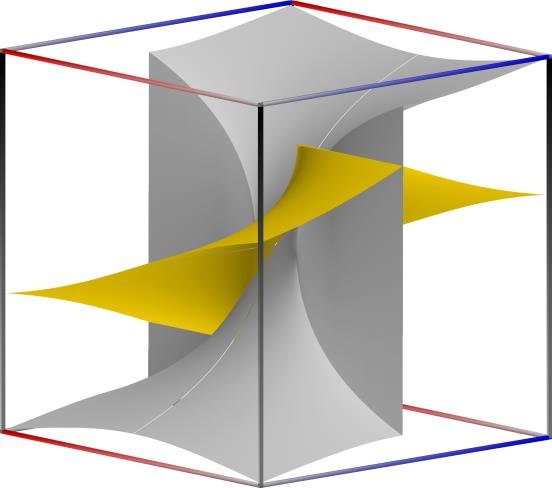
\includegraphics[height=8cm, width=8cm]{Charts/jpg/CplxAsinhBoth.jpg} }}%
	\qquad
	\subfloat[Magnitude and phase (color-coded), $z_{\text{min}}=0$. Camera angles are $\theta = 35\degree$ and $\phi = -112\degree$.]{{\includegraphics[height=8cm, width=8cm]{Charts/jpg/CplxAsinhMag.jpg} }}%
	\caption[Complex Inverse Hyperbolic Sine]{Surface plots of $z = \text{asinh}(x + iy)$, $-3 \leq x \leq 3$ (blue axis), $-2 \pi \leq y \leq 2\pi$ (red axis), $z_{\text{min}} \leq z \leq 10$ (black axis). $z$ values are truncated at $\pm 10$. There is a branch cut along the negative real axis. Orthographic camera. See section \ref{Graphics: Surface plots of complex functions} for more information about charts for complex functions.} 
	\label{fig:Complex Inverse Hyperbolic Sine}%
\end{figure}




\newpage
\subsection{\texorpdfstring{$\text{Inverse Hyperbolic Cosine: acosh}(z)$}{acosh}}

\begin{mpFunctionsExtract}
	\mpWorksheetFunctionOneNotImplemented
	{ACOSH? mpNum? the value of the hyperbolic arc-cosine  of $x$ in radians.}
	{x? mpNum? A real number.}
\end{mpFunctionsExtract}

\vspace{0.6cm}


\begin{mpFunctionsExtract}
	\mpFunctionOne
	{acosh? mpNum? the inverse complex hyperbolic cosine of $z$}
	{z? mpNum? A complex number.}
\end{mpFunctionsExtract}

\vspace{0.3cm}
The function \textsf{cplxACosh$(z)$} returns the inverse complex hyperbolic cosine of $z$: 
\begin{equation}
	\text{arccosh}(z) = \pm i \text{ arccos}(z),
\end{equation}
where $\text{arccos}(z)$ is defined in section \ref{inverse complex cosine}

Computes the inverse hyperbolic cosine of $x$, $\cosh^{-1}(x)=\log(x+\sqrt{x+1}\sqrt{x-1})$.

\begin{figure}[ht]%
	\centering
	\subfloat[Real ("silver") and imaginary ("gold") component, $z_{\text{min}}=-10$. Camera angles are $\theta = 135\degree$ and $\phi = -12\degree$.]{{\includegraphics[height=8cm, width=8cm]{Charts/jpg/CplxAcoshBoth.jpg} }}%
	\qquad
	\subfloat[Magnitude and phase (color-coded), $z_{\text{min}}=0$. Camera angles are $\theta = 35\degree$ and $\phi = -112\degree$.]{{\includegraphics[height=8cm, width=8cm]{Charts/jpg/CplxAcoshMag.jpg} }}%
	\caption[Complex Inverse Hyperbolic Cosine]{Surface plots of $z = \text{acosh}(x + iy)$, $-3 \leq x \leq 3$ (blue axis), $-2 \pi \leq y \leq 2\pi$ (red axis), $z_{\text{min}} \leq z \leq 10$ (black axis). $z$ values are truncated at $\pm 10$. There is a branch cut along the negative real axis. Orthographic camera. See section \ref{Graphics: Surface plots of complex functions} for more information about charts for complex functions.} 
	\label{fig:Complex Inverse Hyperbolic Cosine}%
\end{figure}


\newpage
\subsection{\texorpdfstring{$\text{Inverse Hyperbolic Tangent: atanh}(z)$}{atanh}}

\begin{mpFunctionsExtract}
	\mpWorksheetFunctionOneNotImplemented
	{ATANH? mpNum? the value of the hyperbolic arc-tangent  of $x$ in radians.}
	{x? mpNum? A real number.}
\end{mpFunctionsExtract}


\vspace{0.6cm}


\begin{mpFunctionsExtract}
	\mpFunctionOne
	{atanh? mpNum? the inverse complex hyperbolic tangent of $z$}
	{z? mpNum? A complex number.}
\end{mpFunctionsExtract}

\vspace{0.3cm}
The function \textsf{cplxATanh$(z)$} returns the inverse complex hyperbolic tangent of $z$: 
\begin{equation}
	\text{arctanh}(z) = -i \text{ arctan}(z),
\end{equation}
where $\text{arctan}(z)$ is defined in section \ref{inverse complex tangent}

Computes the inverse hyperbolic tangent of $x$, $\tanh^{-1}(x)=\tfrac{1}{2} (\log(1+x) - \log(1+x))$.


\begin{figure}[ht]%
	\centering
	\subfloat[Real ("silver") and imaginary ("gold") component, $z_{\text{min}}=-10$. Camera angles are $\theta = 135\degree$ and $\phi = -12\degree$.]{{\includegraphics[height=8cm, width=8cm]{Charts/jpg/CplxAtanhBoth.jpg} }}%
	\qquad
	\subfloat[Magnitude and phase (color-coded), $z_{\text{min}}=0$. Camera angles are $\theta = 35\degree$ and $\phi = -112\degree$.]{{\includegraphics[height=8cm, width=8cm]{Charts/jpg/CplxAtanhMag.jpg} }}%
	\caption[Complex Inverse Hyperbolic Tangent]{Surface plots of $z = \text{atanh}(x + iy)$, $-3 \leq x \leq 3$ (blue axis), $-2 \pi \leq y \leq 2\pi$ (red axis), $z_{\text{min}} \leq z \leq 10$ (black axis). $z$ values are truncated at $\pm 10$. There is a branch cut along the negative real axis. Orthographic camera. See section \ref{Graphics: Surface plots of complex functions} for more information about charts for complex functions.} 
	\label{fig:Complex Inverse Hyperbolic Tangent}%
\end{figure}



\newpage
\subsection{\texorpdfstring{$\text{Inverse Hyperbolic Cotangent: acoth}(z)$}{acoth}}
\label{inverse complex hyperbolic cotangent}

\begin{mpFunctionsExtract}
	\mpWorksheetFunctionOneNotImplemented
	{ACOTH? mpNum? the value of the hyperbolic arc-cotangent  of $x$ in radians.}
	{x? mpNum? A real number.}
\end{mpFunctionsExtract}

\vspace{0.6cm}



\begin{mpFunctionsExtract}
	\mpFunctionOne
	{acoth? mpNum? the inverse complex hyperbolic cotangent of $z$}
	{z? mpNum? A complex number.}
\end{mpFunctionsExtract}

\vspace{0.3cm}
The function \textsf{cplxACoth$(z)$} returns the inverse complex hyperbolic cotangent of $z$: 
\begin{equation}
	\text{arctanh}(z) = i \text{ arctan}(iz),
\end{equation}
where $\text{arctan}(z)$ is defined in section \ref{inverse complex cotangent}



Computes the inverse hyperbolic cotangent of $x$, $\text{coth}^{-1}(x) = \tanh^{-1}(1/x)$

\begin{figure}[ht]%
	\centering
	\subfloat[Real ("silver") and imaginary ("gold") component, $z_{\text{min}}=-10$. Camera angles are $\theta = 135\degree$ and $\phi = -12\degree$.]{{\includegraphics[height=8cm, width=8cm]{Charts/jpg/CplxAcothBoth.jpg} }}%
	\qquad
	\subfloat[Magnitude and phase (color-coded), $z_{\text{min}}=0$. Camera angles are $\theta = 35\degree$ and $\phi = -112\degree$.]{{\includegraphics[height=8cm, width=8cm]{Charts/jpg/CplxAcothMag.jpg} }}%
	\caption[Complex Inverse Hyperbolic Cotangent]{Surface plots of $z = \text{acoth}(x + iy)$, $-3 \leq x \leq 3$ (blue axis), $-2 \pi \leq y \leq 2\pi$ (red axis), $z_{\text{min}} \leq z \leq 10$ (black axis). $z$ values are truncated at $\pm 10$. There is a branch cut along the negative real axis. Orthographic camera. See section \ref{Graphics: Surface plots of complex functions} for more information about charts for complex functions.} 
	\label{fig:Complex Inverse Hyperbolic Cotangent}%
\end{figure}



\subsection{asech(x)}
Computes the inverse hyperbolic secant of $x$, $\text{sech}^{-1}(x) = \cosh^{-1}(1/x)$



\subsection{acsch(x)}
Computes the inverse hyperbolic cosecant of $x$, $\text{csch}^{-1}(x) = \sinh^{-1}(1/x)$




\newpage
\section{Elementary Functions of Mathematical Physics}

\subsection{\texorpdfstring{$\text{Bessel Function }J_{\nu}(x)$}{Bessel Function Jnu}}
\nomenclature{$J_{\nu}(z)$}{Bessel function of the first kind of real order $\nu$}

\label{BESSELJnu} 
\begin{mpFunctionsExtract}
	\mpWorksheetFunctionTwoNotImplemented
	{BESSELJ? mpNum? $J_{\nu}(z)$, the Bessel function of the first kind of real order $\nu$.}
	{x? mpNum? A real number.}
	{$\nu$? mpNum? A real number.}
\end{mpFunctionsExtract}

\vspace{0.3cm}
$J_{\nu}(z)$, the Bessel function of the first kind of order $\nu$, is defined as
\begin{equation}
	J_{\nu}(x)  = \left(\tfrac{1}{2}x\right)^{\nu}  \sum_{k=0}^\infty (-1)^k \frac{(x^2 / 4)^k}{k! \Gamma(\nu+k+1)}
\end{equation}




\subsection{\texorpdfstring{$\text{Bessel Function }Y_{\nu}(x)$}{Ynux}}
\nomenclature{$Y_{\nu}(z)$}{Bessel function of the second kind of real order $\nu$}
\label{BESSELYnu} 

\begin{mpFunctionsExtract}
	\mpWorksheetFunctionTwoNotImplemented
	{BESSELY? mpNum? $Y_{\nu}(z)$, the Bessel function of the second kind of order $\nu$.}
	{x? mpNum? A real number.}
	{$\nu$? mpNum? A real number.}
\end{mpFunctionsExtract}

\vspace{0.3cm}
$Y_{\nu}(z)$, the Bessel function of the second kind of order $\nu$, is defined as
\begin{equation}
	Y_{\nu}(x)  = \frac{J_{\nu}(x) \cos(\nu \pi) - J_{-\nu}(x)}{ \sin(\nu \pi)}
\end{equation}



\subsection{\texorpdfstring{$\text{Bessel Function }I_{\nu}(x)$}{Bessel Function Inu}}
\nomenclature{$I_{\nu}(z)$}{Modified Bessel function of the first kind of real order $\nu$}
\label{BESSELInu} 

\begin{mpFunctionsExtract}
	\mpWorksheetFunctionTwoNotImplemented
	{BESSELI? mpNum? $J_{\nu}(z)$, the Bessel function of the first kind of real order $\nu$.}
	{x? mpNum? A real number.}
	{$\nu$? mpNum? A real number.}
\end{mpFunctionsExtract}

\vspace{0.3cm}
This function returns the modified Bessel function $I_{\nu}(z)$ of the first kind of order $\nu$, defined as
\begin{equation}
	I_{\nu}(z)  = \frac{z}{2}  \sum_{j=0}^\infty \frac{(z^2 / 4)^j}{j! \Gamma(\nu+j+1)}
\end{equation}




\subsection{\texorpdfstring{$\text{Bessel Function }K_{\nu}(x)$}{Bessel Function Knu}}
\nomenclature{$K_{\nu}(z)$}{Modified Bessel function of the second kind of real order $\nu$}
\label{BESSELKnu} 

\begin{mpFunctionsExtract}
	\mpWorksheetFunctionTwoNotImplemented
	{BESSELK? mpNum?  $K_{\nu}(x)$, the modified Bessel function of the second kind of order $\nu$.}
	{x? mpNum? A real number.}
	{$\nu$? mpNum? A real number.}
\end{mpFunctionsExtract}

\vspace{0.3cm}
This function returns $K_{\nu}(z)$, the modified Bessel function of the second kind of order $\nu$, defined as
\begin{equation}
	K_{\nu}(x)  = \frac{\pi}{2} \frac{I_{-\nu}(x)) - I_{\nu}(x)}{ \sin(\nu \pi)}
\end{equation}




\vspace{0.6cm}
\begin{mpFunctionsExtract}
	\mpWorksheetFunctionOneNotImplemented
	{ERF? mpNum? the value of the error function.}
	{x? mpNum? A real number.}
\end{mpFunctionsExtract}

\vspace{0.6cm}
\begin{mpFunctionsExtract}
	\mpWorksheetFunctionOneNotImplemented
	{ERF.PRECISE? mpNum? the value of the error function.}
	{x? mpNum? A real number.}
\end{mpFunctionsExtract}

\vspace{0.3cm}
The error function is defined by
\begin{equation}
	\text{erf}(x) = \frac{2}{\sqrt{\pi}} \int_0^x e^{-x^2} dt,
\end{equation}



\subsection{Complementary Error Function}
\label{Complementary Error Function}

\vspace{0.6cm}
\begin{mpFunctionsExtract}
	\mpWorksheetFunctionOneNotImplemented
	{ERFC? mpNum? the value of the complementary error function.}
	{x? mpNum? A real number.}
\end{mpFunctionsExtract}

\vspace{0.6cm}
\begin{mpFunctionsExtract}
	\mpWorksheetFunctionOneNotImplemented
	{ERFC.PRECISE? mpNum? the value of the complementary error function.}
	{x? mpNum? A real number.}
\end{mpFunctionsExtract}

\vspace{0.3cm}
The complementary error function is defined by
\begin{equation}
	\text{erfc}(x) = 1-\text{erf}(x) = \frac{2}{\sqrt{\pi}} \int_x^\infty e^{-x^2} dt,
\end{equation}




\subsection{\texorpdfstring{$\text{Gamma function }\Gamma(x)$}{TGamma}}
\nomenclature{$\Gamma(x)$}{Gamma Function}
\label{GammaFunction}

\vspace{0.6cm}
\begin{mpFunctionsExtract}
	\mpWorksheetFunctionOneNotImplemented
	{GAMMA? mpNum? the gamma function for $x \neq 0, -1, -2,\ldots$.}
	{x? mpNum? A real number.}
\end{mpFunctionsExtract}

\vspace{0.3cm}
The gamma function for $x \neq 0, -1, -2,\ldots$ is defined by
\begin{equation}
	\Gamma(x)  = \int_{0}^{\infty} t^{x-1} e^{-t} dt \quad (x>0),
\end{equation}
and by analytic continuation if $x<0$, using the reflection formula
\begin{equation}
	\Gamma(x) \Gamma(1-x)  = \pi / \sin(\pi x).
\end{equation}



%\begin{mpFunctionsExtract}
	
	\begin{mpFunctionsExtract}
		\mpWorksheetFunctionOneNotImplemented
		{GAMMALN? mpNum? the logarithm of the gamma function.}
		{x? mpNum? A real number.}
	\end{mpFunctionsExtract}
	
	\vspace{0.6cm}
	
	\begin{mpFunctionsExtract}
		\mpWorksheetFunctionOneNotImplemented
		{GAMMALN.PRECISE? mpNum? the logarithm of the gamma function.}
		{x? mpNum? A real number.}
	\end{mpFunctionsExtract}
	
	
	
	\subsection{Beta Function B(a,b)}
	\label{BetaFunction}
	\begin{mpFunctionsExtract}
		\mpFunctionTwoNotImplemented
		{Beta? mpNum? the Beta function.}
		{a? mpNum? A real number.}
		{b? mpNum? A real number.}
	\end{mpFunctionsExtract}
	
	\vspace{0.3cm}
	This function computes $B(a,b)$ for $a, b \neq 0, -1, -2, \ldots$. 
	
	
	

\newpage
\section{Factorial and Related Functions}
\label{NumbertheoreticFunctions}
\subsection{Factorial}


\vspace{0.6cm}
\begin{mpFunctionsExtract}
	\mpWorksheetFunctionOneNotImplemented
	{FACT? Integer?  $n!$, the factorial of $n$}
	{n? Integer? An Integer.}
\end{mpFunctionsExtract}



\subsection{Double Factorial}

\begin{mpFunctionsExtract}
	\mpWorksheetFunctionOneNotImplemented
	{FACTDOUBLE? Integer?  $n!!$, the double factorial of $n$}
	{n? Integer? An Integer.}
\end{mpFunctionsExtract}




\subsection{Binomial Coefficient, Combinations}


\vspace{0.6cm}
\begin{mpFunctionsExtract}
	\mpWorksheetFunctionTwoNotImplemented
	{COMBIN? Integer? the binomial coefficient}
	{n? Integer? An Integer.}
	{k? Integer? An Integer.}
\end{mpFunctionsExtract}

\vspace{0.3cm}
Returns the binomial coefficient, $\binom{n}{k}$. Negative values of $n$ are supported, using the identity
\begin{equation}
	\binom{-n}{k} = (-1)^k \binom{n+k-1}{k}.
\end{equation}


\vspace{0.6cm}
\begin{mpFunctionsExtract}
	\mpWorksheetFunctionTwoNotImplemented
	{COMBINA? Integer? the binomial coefficient}
	{n? Integer? An Integer.}
	{k? Integer? An Integer.}
\end{mpFunctionsExtract}




\subsection{Multinomial}

\begin{mpFunctionsExtract}
	\mpWorksheetFunctionOneNotImplemented
	{MULTINOMIAL? mpReal? the multinomial}
	{a[]? mpReal? An array of integers.}
\end{mpFunctionsExtract}

\vspace{0.3cm}
Returns the multinomial, defined as  the ratio of the factorial of a sum of values to the product of factorials:
\begin{equation}
	\textsf{MULTINOMIAL}(a_1,a_2,\ldots,a_n) = \frac{(a_1+a_2+\ldots+a_n)!}{a_1! a_2! \ldots a_n!}
\end{equation}





\subsection{Permutations}

\begin{mpFunctionsExtract}
	\mpWorksheetFunctionTwoNotImplemented
	{PERMUT? Integer? the number of permutations for a given number $k$ of objects that can be selected from $n$ objects.}
	{n? Integer? An Integer.}
	{k? Integer? An Integer.}
\end{mpFunctionsExtract}

\vspace{0.3cm}
\begin{mpFunctionsExtract}
	\mpWorksheetFunctionTwoNotImplemented
	{PERMUTATIONA? Integer? the number of permutations for a given number $k$ of objects that can be selected from $n$ objects.}
	{n? Integer? An Integer.}
	{k? Integer? An Integer.}
\end{mpFunctionsExtract}

\vspace{0.3cm}
Returns the number of permutations for a given number $k$ of objects that can be selected from $n$ objects. A permutation is any set or subset of objects or events where internal order is significant.
\begin{equation}
	\textsf{PERMUT}(n, k) = \frac{n!}{(n-k)!}
\end{equation}



\subsection{Greatest Common Divisor (GCD)}


\vspace{0.6cm}
\begin{mpFunctionsExtract}
	\mpWorksheetFunctionTwoNotImplemented
	{GCD? Integer? the greatest common divisor of $n_1$ and $n_2$}
	{n1? Integer? An Integer.}
	{n2? Integer? An Integer.}
\end{mpFunctionsExtract}

\vspace{0.3cm}
The result is always positive even if
one or both input operands are negative. Except if both inputs are zero; then this function
defines \textsf{intGcd}(0, 0) = 0.



\subsection{Least Common Multiple (LCM)}


\vspace{0.6cm}
\begin{mpFunctionsExtract}
	\mpWorksheetFunctionTwoNotImplemented
	{LCM? Integer? the least common multiple of $n_1$ and $n_2$.}
	{n1? Integer? An Integer.}
	{n2? Integer? An Integer.}
\end{mpFunctionsExtract}

\vspace{0.3cm}
Returns the least common multiple of $n_1$ and $n_2$. The returned value is always positive, irrespective of the signs of $n_1$ and $n_2$. The returned value  will be zero if either $n_1$ or $n_2$ is zero.




\chapter{Linear Algebra}

\section{Multiple Linear Regression}



\subsection{Determinant}

\begin{mpFunctionsExtract}
	\mpWorksheetFunctionOneNotImplemented
	{MDETERM? mpNum? the matrix determinant of a numeric array $X$ with an equal number of rows and columns.}
	{X? mpNum[]? A matrix of real numbers.}
\end{mpFunctionsExtract}





\subsection{Inverse}

\begin{mpFunctionsExtract}
	\mpWorksheetFunctionOneNotImplemented
	{MINVERSE? mpNum? the  inverse matrix for the matrix stored in the numeric array  $X$ with an equal number of rows and columns.}
	{X? mpNum[]? A matrix of real numbers.}
\end{mpFunctionsExtract}


Negative powers will calculate the inverse:

\lstset{language={Python}}
\begin{lstlisting}
>>> A**-1
matrix(
[['-2.0', '1.0'],
['1.5', '-0.5']])
>>> nprint(A * A**-1, 3)
[ 1.0 1.08e-19]
[-2.17e-19 1.0]
\end{lstlisting}






\subsection{LinEst}
\label{LinEst}

\begin{mpFunctionsExtract}
	\mpWorksheetFunctionFourNotImplemented
	{LINEST? mpNumList? information obtained by performing multiple liner regression.}
	{Y? mpNum[]? An array of real numbers.}
	{X? mpNum[]? An array of real numbers.}
	{Const? Boolean? A logical value.}
	{Stats? Boolean? A logical value.}
\end{mpFunctionsExtract}



\vspace{0.3cm}
The LINEST function calculates the statistics for a line by using the "least squares" method to calculate a straight line that best fits your data, and then returns an array that describes the line. 

You can also combine LINEST with other functions to calculate the statistics for other types of models that are linear in the unknown parameters, including polynomial, logarithmic, exponential, and power series. Because this function returns an array of values, it must be entered as an array formula. Instructions follow the examples in this article.

This function can also be used to perform multiple linear regression.

This function needs a detailed explanation.



\subsection{TREND}

\begin{mpFunctionsExtract}
	\mpWorksheetFunctionFourNotImplemented
	{TREND? mpNumList? values along a linear trend.}
	{Y? mpNum[]? An array of real numbers.}
	{X? mpNum[]? An array of real numbers.}
	{NewX? mpNum[]? An array of real numbers.}
	{Const? Boolean? A logical value.}
\end{mpFunctionsExtract}

\vspace{0.3cm}
Returns values along a linear trend. Fits a straight line (using the method of least squares) to the arrays $Y$ and $X$. Returns the y-values along that line for the array of $NewX$ that you specify.

For information about how Microsoft Excel fits a line to data, see LINEST.
You can use TREND for polynomial curve fitting by regressing against the same variable raised to different powers. For example, suppose column A contains y-values and column B contains x-values. You can enter $x^2$ in column C, $x^3$ in column D, and so on, and then regress columns B through D against column A.

Formulas that return arrays must be entered as array formulas.



\newpage
\section{Exponential Growth Curves}

\subsection{LogEst}

\begin{mpFunctionsExtract}
	\mpWorksheetFunctionFourNotImplemented
	{LOGEST? mpNumList? an exponential curve that fits your data and returns an array of values that describes the curve.}
	{Y? mpNum[]? An array of real numbers.}
	{X? mpNum[]? An array of real numbers.}
	{Const? Boolean? A logical value.}
	{Stats? Boolean? A logical value.}
\end{mpFunctionsExtract}

\vspace{0.3cm}
In regression analysis, calculates an exponential curve that fits your data and returns an array of values that describes the curve. Because this function returns an array of values, it must be entered as an array formula.

This function does not perform a non-linear estimation.



\subsection{Growth}

\begin{mpFunctionsExtract}
	\mpWorksheetFunctionFourNotImplemented
	{GROWTH? mpNumList? predicted exponential growth by using existing data.}
	{Y? mpNum[]? An array of real numbers.}
	{X? mpNum[]? An array of real numbers.}
	{NewX? mpNum[]? An array of real numbers.}
	{Const? Boolean? A logical value.}
\end{mpFunctionsExtract}

\vspace{0.3cm}
\textsf{GROWTH} returns the $y$-values for a series of new $x$-values that you specify by using existing $x$-values and $y$-values. You can also use the \textsf{GROWTH} worksheet function to fit an exponential curve to existing $x$-values and $y$-values.



\newpage
\section{Norms}
Sometimes you need to know how 'large' a matrix or vector is. Due to their multidimensional nature it is not possible to compare them, but there are several functions to map a matrix or a vector to a positive real number, the so called norms.

\vpara
\begin{mpFunctionsExtract}
	\mpFunctionTwo
	{norm? mpNumList? the entrywise $p$-norm of an iterable x, i.e. the vector norm.}
	{Y? mpNum[]? An array of real numbers.}
	{Keywords? String?  p=2.}
\end{mpFunctionsExtract}


norm(ctx, x, p=2)
Gives the entrywise $p$-norm of an iterable x, i.e. the vector norm 

\begin{equation}
	\left( \sum_k |x_k|^p \right)^{1/p},
\end{equation}
for any given $1 \leq p \leq \infty$.

Special cases:

If x is not iterable, this just returns absmax(x).

p=1 gives the sum of absolute values.

p=2 is the standard Euclidean vector norm.

p=inf gives the magnitude of the largest element.

For x a matrix, p=2 is the Frobenius norm. For operator matrix norms, use mnorm() instead.

You can use the string 'inf' as well as float('inf') or mpf('inf') to specify the infinity norm.

\vpara
\textbf{Examples}

\lstset{language={Python}}
\begin{lstlisting}
>>> from mpFormulaPy import *
>>> mp.dps = 15; mp.pretty = False
>>> x = matrix([-10, 2, 100])
>>> norm(x, 1)
mpf('112.0')
>>> norm(x, 2)
mpf('100.5186549850325')
>>> norm(x, inf)
mpf('100.0')
\end{lstlisting}


\vspace{0.6cm}

\begin{mpFunctionsExtract}
	\mpFunctionTwo
	{mnorm? mpNumList? the matrix (operator) $p$-norm of A. Currently p=1 and p=inf are supported.}
	{A? mpNum[]? An array of real numbers.}
	{Keywords? String?  p=1.}
\end{mpFunctionsExtract}


mnorm(ctx, A, p=1)

Gives the matrix (operator) $p$-norm of A. Currently p=1 and p=inf are supported:

p=1 gives the 1-norm (maximal column sum)

p=inf gives the -norm (maximal row sum). You can use the string 'inf' as well as float('inf') or mpf('inf')

p=2 (not implemented) for a square matrix is the usual spectral matrix norm, i.e. the largest singular value.

p='f' (or 'F', 'fro', 'Frobenius', 'frobenius') gives the Frobenius norm, which is the elementwise 2-norm. The Frobenius norm is an approximation of the spectral norm and satisfies

\begin{equation}
	\frac{1}{\sqrt{\text{rank}(A)}} ||A||_F \leq ||A||_2 \leq ||A||_F.
\end{equation}

The Frobenius norm lacks some mathematical properties that might be expected of a norm.

For general elementwise $p$-norms, use norm() instead.

\vpara
\textbf{Examples}

\lstset{language={Python}}
\begin{lstlisting}
>>> from mpFormulaPy import *
>>> mp.dps = 15; mp.pretty = False
>>> A = matrix([[1, -1000], [100, 50]])
>>> mnorm(A, 1)
mpf('1050.0')
>>> mnorm(A, inf)
mpf('1001.0')
>>> mnorm(A, 'F')
mpf('1006.2310867787777')
\end{lstlisting}





\newpage
\section{Decompositions}


\begin{mpFunctionsExtract}
	\mpFunctionTwo
	{cholesky? mpNum? the Cholesky decomposition of a symmetric positive-definite matrix $A$.}
	{A? mpNum[]? A symmetric matrix.}
	{Keywords? String?  tol=None.}
\end{mpFunctionsExtract}


cholesky(ctx, A, tol=None)

Cholesky decomposition of a symmetric positive-definite matrix $A$. Returns a lower triangular matrix $L$ such that $A=L \times L^T$. More generally, for a complex Hermitian positive-definite matrix, a Cholesky decomposition satisfying $A=L \times L^H$ is returned.

\vpara
The Cholesky decomposition can be used to solve linear equation systems twice as efficiently as LU decomposition, or to test whether $A$ is positive-definite.

\vpara
The optional parameter tol determines the tolerance for verifying positive-definiteness.

\vpara
\textbf{Examples}

Cholesky decomposition of a positive-definite symmetric matrix:

\lstset{language={Python}}
\begin{lstlisting}
>>> from mpFormulaPy import *
>>> mp.dps = 25; mp.pretty = True
>>> A = eye(3) + hilbert(3)
>>> nprint(A)
[ 2.0 0.5 0.333333]
[ 0.5 1.33333 0.25]
[0.333333 0.25 1.2]
>>> L = cholesky(A)
>>> nprint(L)
[ 1.41421 0.0 0.0]
[0.353553 1.09924 0.0]
[0.235702 0.15162 1.05899]
>>> chop(A - L*L.T)
[0.0 0.0 0.0]
[0.0 0.0 0.0]
[0.0 0.0 0.0]
\end{lstlisting}

Cholesky decomposition of a Hermitian matrix:

\lstset{language={Python}}
\begin{lstlisting}
>>> A = eye(3) + matrix([[0,0.25j,-0.5j],[-0.25j,0,0],[0.5j,0,0]]
>>> L = cholesky(A)
>>> nprint(L)
[ 1.0 0.0 0.0]
[(0.0 - 0.25j) (0.968246 + 0.0j) 0.0]
[ (0.0 + 0.5j) (0.129099 + 0.0j) (0.856349 + 0.0j)]
>>> chop(A - L*L.H)
[0.0 0.0 0.0]
[0.0 0.0 0.0]
[0.0 0.0 0.0]
\end{lstlisting}

Attempted Cholesky decomposition of a matrix that is not positive definite:

\lstset{language={Python}}
\begin{lstlisting}
>>> A = -eye(3) + hilbert(3)
>>> L = cholesky(A)
Traceback (most recent call last):
...
ValueError: matrix is not positive-definite
\end{lstlisting}




\newpage
\section{Linear Equations}


\begin{mpFunctionsExtract}
	\mpFunctionThree
	{lu\_solve? mpNum? solves a linear equation system using a LU decomposition.}
	{A? mpNum[]? A symmetric matrix.}
	{b? mpNum[]? A symmetric matrix.}	
	{Keywords? String?  tol=None.}
\end{mpFunctionsExtract}


You can for example solve the linear equation system using a LU decomposition:

\lstset{language={Python}}
\begin{lstlisting}
x + 2*y = -10
3*x + 4*y = 10
\end{lstlisting}

using lu\_solve:

\lstset{language={Python}}
\begin{lstlisting}
>>> A = matrix([[1, 2], [3, 4]])
>>> b = matrix([-10, 10])
>>> x = lu_solve(A, b)
>>> x
matrix(
[['30.0'],
['-20.0']])
\end{lstlisting}


\begin{mpFunctionsExtract}
	\mpFunctionFour
	{residual? mpNum? the residual  $||Ax-b||$.}
	{A? mpNum[]? A square matrix.}
	{b? mpNum[]? A vector.}
	{x? mpNum[]? A vector.}		
	{Keywords? String?  tol=None.}
\end{mpFunctionsExtract}


Calculates the residual  $||Ax-b||$:

\lstset{language={Python}}
\begin{lstlisting}
>>> residual(A, x, b)
matrix(
[['3.46944695195361e-18'],
['3.46944695195361e-18']])
>>> str(eps)
'2.22044604925031e-16'
\end{lstlisting}

As you can see, the solution is quite accurate. The error is caused by the inaccuracy of the internal floating point arithmetic. Though, it is even smaller than the current machine epsilon, which basically means you can trust the result.

If you need more speed, use NumPy, or use fp instead mp matrices and methods:

\lstset{language={Python}}
\begin{lstlisting}
>>> A = fp.matrix([[1, 2], [3, 4]])
>>> b = fp.matrix([-10, 10])
>>> fp.lu_solve(A, b)
matrix(
[['30.0'],
['-20.0']])
\end{lstlisting}

lu\_solve accepts overdetermined systems. It is usually not possible to solve such systems, so the residual is minimized instead. Internally this is done using Cholesky decomposition to compute a least squares approximation. This means that that lu\_solve will square the errors. If you cannot afford this, use qr\_solve instead. It is twice as slow but more accurate, and it calculates the residual automatically.



\newpage
\section{Matrix Factorization}

\begin{mpFunctionsExtract}
	\mpFunctionTwo
	{lu? mpNum? an explicit LU factorization of a matrix, returning P, L, U}
	{A? mpNum[]? A square matrix.}
	{Keywords? String?  tol=None.}
\end{mpFunctionsExtract}


The function lu computes an explicit LU factorization of a matrix:

\lstset{language={Python}}
\begin{lstlisting}
>>> P, L, U = lu(matrix([[0,2,3],[4,5,6],[7,8,9]]))
>>> print P
[0.0 0.0 1.0]
[1.0 0.0 0.0]
[0.0 1.0 0.0]
>>> print L
[ 1.0 0.0 0.0]
[ 0.0 1.0 0.0]
[0.571428571428571 0.214285714285714 1.0]
>>> print U
[7.0 8.0 9.0]
[0.0 2.0 3.0]
[0.0 0.0 0.214285714285714]
>>> print P.T*L*U
[0.0 2.0 3.0]
[4.0 5.0 6.0]
[7.0 8.0 9.0]
\end{lstlisting}




\begin{mpFunctionsExtract}
	\mpFunctionTwo
	{qr? mpNum? an explicit QR factorization of a matrix, returning Q, R}
	{A? mpNum[]? A square matrix.}
	{Keywords? String?  tol=None.}
\end{mpFunctionsExtract}

\vpara
Examples:

\lstset{language={Python}}
\begin{lstlisting}
>>> A = matrix([[1, 2], [3, 4], [1, 1]])
>>> Q, R = qr(A)
>>> print Q
[-0.301511344577764 0.861640436855329 0.408248290463863]
[-0.904534033733291 -0.123091490979333 -0.408248290463863]
[-0.301511344577764 -0.492365963917331 0.816496580927726]
>>> print R
[-3.3166247903554 -4.52267016866645]
[ 0.0 0.738548945875996]
[ 0.0 0.0]
>>> print Q * R
[1.0 2.0]
[3.0 4.0]
[1.0 1.0]
>>> print chop(Q.T * Q)
[1.0 0.0 0.0]
[0.0 1.0 0.0]
[0.0 0.0 1.0]
\end{lstlisting}






\newpage
\section{Time Series}
%\lipsum[1]

\subsection{Exponential Smoothing}
\label{Exponential Smoothing}
This section covers Exponential Smoothing, as implemented in Excel Toolpak


\subsection{Moving Average}
\label{Moving Average}
This section covers Moving Average, as implemented in Excel Toolpak





\chapter{Distribution Functions}

\section{Introduction to Distribution Functions}
\label{DistributionFunctionsIntroduction} 

%\lipsum[1]

This is a citation~\citet{walck_2007}, and some more.

This is a citation~\citet{VanHauwermeiren_2009}, and some more.

This is a citation~\citet{Rinne_book_2008}, and some more.

This is a citation~\citet{Johnson_1994}, and some more.

This is a citation~\citet{Johnson_1995}, and some more.
\nomenclature{pmf}{probability mass function}%
\nomenclature{pdf}{probability density function}%
\nomenclature{CDF}{cumulative distribution function}%


See also \cite{Monahan_2011}

See also \cite{Lange_2010}

See also \cite{Chernick_2008}

See also \cite{Cheney_2008}


\subsection{Continuous Distribution Functions}

Continuous random number distributions are defined by a probability density function, $p(x)$, such that the probability of $x$ occurring in the infinitesimal range $x$ to $x +dx$ is $p\ dx$. The cumulative distribution function for the lower tail $P(x)$ gives the probability of a variate taking a value less than $x$, and the cumulative distribution function for the upper tail $Q(x)$ gives the probability of a variate taking a value greater than $x$. 

The upper and lower cumulative distribution functions are related by $P(x) + Q(x) = 1$ and satisfy $0 \leq P(x) \leq 1, 0 \leq Q(x) \leq 1$. The inverse cumulative distributions, $x = P-1(P)$ and $x = Q-1(Q)$ give the values of $x$ which correspond to a specific value of $P$ or $Q$. They can be used to find confidence limits from probability values. 



\subsection{Discrete Distribution Functions}

For discrete distributions the probability of sampling the integer value $k$ is given by $p(k)$. The cumulative distribution for the lower tail $P(k)$ of a discrete distribution is defined as the sum over the allowed range of the distribution less than or equal to $k$. The cumulative distribution for the upper tail of a discrete distribution $Q(k)$ is defined as the sum of probabilities for all values greater than $k$. These two definitions satisfy the identity $P(k) + Q(k) = 1$. If the range of the distribution is 1 to $n$ inclusive then $P(n) = 1$, $Q(n) = 0$ while $P(1) = p(1)$, $Q(1) = 1 - p(1)$. 


\newpage
\subsection{Commonly Used Function Types}
\label{Commonly Used Distribution Function Types}

\subsubsection{Functions returning pdf, CDF, and related information}
\label{Functions returning pdf, CDF, and related information}
These functions have the form \textsf{?Dist($x$; [Parameters;], OutputString)}.
Here 

"?" is a placeholder for the name of the distribution, 

"$x$" is the value for which we want to calculate the pdf, CDF etc, 

"[Parameters;]" denote any parameters (like degrees of freedom) of the distribution, and 

"OutputString" specifies the computed results which will be returned. This can be any of the following:

\begin{itemize}
	\item \textbf{pdf}: the probability density function
	\item \textbf{P}: the cumulative distribution function (CDF)
	\item \textbf{Q}: the complement of cumulative distribution function (CDF)
	\item \textbf{logpdf}: the logarithm of the probability density function
	\item \textbf{logP}: the logarithm of the cumulative distribution function (CDF)
	\item \textbf{logQ}: the logarithm of the complement of cumulative distribution function (CDF)
	\item \textbf{h}: hazard function
	\item \textbf{H}: cumulative hazard function
\end{itemize}


\vspace{0.3cm}
As an example, for Student's t-distribution, a "T" is used to specify the name of the distibution, and there is just one distribution parameter, $\nu$, the degrees of freedom. Therefore,  the function has the form

\vspace{0.3cm}
\textsf{TDist($x$ As nmNum; $\nu$ As mpNum, OutputString As String) As mpNumList}, 

\vspace{0.3cm}
and an actual call to the function, requesting the pdf, CDF, and the complement of the CDF for $x=2.3$ and $\nu=22$ could be

\lstset{language={[Visual]Basic}}
\begin{lstlisting}
Result = TDist(2.3, 22, "pdf + P + Q")
mp.Print Result
\end{lstlisting}
which produces the output

\begin{verbatim}
pdf: 0.434234342343434
P: 0.943453463453453
Q: 0.054564564564236
\end{verbatim}




\newpage
\subsubsection{Functions returning Quantiles}
\label{Functions returning Quantiles}
These functions have the form \textsf{?DistInv(Prob; [Parameters;], OutputString)}.
Here 

"?" is a placeholder for the name of the distribution, 

"Prob" sets the target values for $P$ and $Q$, 

"[Parameters;]" denote any parameters (like degrees of freedom) of the distribution, and 

"OutputString" specifies the computed results which will be returned. This can be any of the following:

\begin{itemize}
	\item \textbf{PInv}: the inverse of the cumulative distribution function (CDF). For discrete distribution, this will be outwardly rounded
	\item \textbf{QInv}: the inverse of the complement of the cumulative distribution function (CDF). For discrete distribution, this will be outwardly rounded
	\item \textbf{P}: the value of the cumulative distribution function (CDF), which has actually been achieved
	\item \textbf{Q}: the value of the complement of the cumulative distribution function (CDF), which has actually been achieved
\end{itemize}


\vspace{0.3cm}
As an example, for Student's t-distribution, a "T" is used to specify the name of the distibution, and there is just one distribution parameter, $\nu$, the degrees of freedom. Therefore,  the function has the form

\vspace{0.3cm}
\textsf{TDistInv($Prob$ As mpNum; $\nu$ As mpNum, OutputString As String) As mpNumList}, 

\vspace{0.3cm}
and an actual call to the function, requesting the inverse of the complement of the CDF for $Prob=0.01$ and $\nu=22$ could be

\lstset{language={[Visual]Basic}}
\begin{lstlisting}
Result = TDistInv(0,01, 22, "QInv")
mp.Print Result
\end{lstlisting}
which produces the output

\begin{verbatim}
QInv: 2.943453463453453
\end{verbatim}


\newpage
\subsubsection{Functions returning moments and related information}
\label{Functions returning moments and related information}
These functions have the form \textsf{?DistInfo([Parameters;], OutputString)}.
Here 

"?" is a placeholder for the name of the distribution, 

"[Parameters;]" denote any parameters (like degrees of freedom) of the distribution, and 

"OutputString" specifies the computed results which will be returned. This can be any of the following:

\begin{itemize}
	\item \textbf{range}: Returns the valid range of the random variable over distribution dist. 
	\item \textbf{support}: 	
	\item \textbf{mode}: Returns the mode of the distribution dist. This function may return a domain\_error if the distribution does not have a defined mode.
	\item \textbf{median}: Returns the median of the distribution dist.
	\item \textbf{mean}: Returns the mean of the distribution dist. This function may return a domain\_error if the distribution does not have a defi ned mean (for e xample the Cauchy distribution).
	\item \textbf{stdev}: Returns the standard deviation of distribution dist.
	This function may return a domain\_error if the distribution does not have a defined standard deviation.
	\item \textbf{variance}: Returns the variance of the distribution dist.
	This function may return a domain\_error if the distribution does not have a defi ned v ariance.
	\item \textbf{skewness}: Returns the skewness of the distribution dist.
	This function may return a domain\_error if the distribution does not have a defined skewness.
	\item \textbf{kurtosis}: Returns the 'proper' kurtosis (normalized fourth moment) of the distribution dist.
	\item \textbf{kurtosis excess}: Returns the kurtosis excess of the distribution dist. kurtosis excess = kurtosis - 3
\end{itemize}



\vspace{0.3cm}
As an example, for Student's t-distribution, a "T" is used to specify the name of the distibution, and there is just one distribution parameter, $\nu$, the degrees of freedom. Therefore,  the function has the form

\vspace{0.3cm}
\textsf{TDistInfo($\nu$ As mpNum, OutputString As String) As mpNumList}, 

\vspace{0.3cm}
and an actual call to the function, requesting the mean, varaince, skewness and kurtosis with $\nu=22$ could be

\lstset{language={[Visual]Basic}}
\begin{lstlisting}
Result = TDistInfo(22, "mean + variance + skewness + kurtosis")
mp.Print Result
\end{lstlisting}
which produces the output

\begin{verbatim}
mean: 0.434234342343434
variance: 0.943453463453453
skewness: 0.054564564564236
kurtosis: 0.6054564564564236
\end{verbatim}









\newpage
\subsubsection{Functions returning Sample Size estimates}
\label{Functions returning Sample Size estimates}
These functions have the form \textsf{?SampleSize(Alpha; Beta; ModifiedNoncentrality; [Parameters;],  OutputString)}.
Here 

"?" is a placeholder for the name of the distribution, 

"Alpha" specifies the confidence level (or Type I error), 

"Beta" specifies the Type I error (or 1 $-$ Power), 

"ModifiedNoncentrality" specifies the (modified) noncentrality parameter of the distribution in a form which does not depend on sample size (which may require a modification compared to the conventional form for stating the noncentrlaity parameter), 

"[Parameters;]" denote any additional parameters of the distribution (if any) which are not a function of the sample size, and 

"OutputString" specifies the computed results which will be returned. This can be any of the following:

\begin{itemize}
	\item \textbf{ExactN}: returns an "exact", i.e. typically non-integer sample size estimate 
	\item \textbf{UpperN}: upper integer sample size estimate
	\item \textbf{LowerN}: lower integer sample size estimate
	\item \textbf{UpperNPower}: actual power when using UpperN
	\item \textbf{LowerNPower}: actual power when using LowerN
\end{itemize}


\vspace{0.3cm}
As an example, for the noncentral  t-distribution, the prefix "NoncentralT" is used to specify the name of the distibution. The distribution parameter $\nu$, the degrees of freedom, which depends on the sample size, and is therefore not included in the parameter list of this function. The modified noncentrality parameter is called $\tilde{\rho} = \Delta/\sigma$. Therefore, the function has the form

\vspace{0.3cm}
\textsf{NoncentralTSampleSize($\alpha$ As mpNum, $\beta$ As mpNum, $\tilde{\rho}$ As mpNum, OutputString As String) As mpNumList}

\vspace{0.3cm}
and an actual call to the function, requesting an upper sample size estimate (and actual power) for $\alpha = 0.95$, $\beta=0.1$ , and $\tilde{\rho} = \Delta/\sigma = 0.6$   would be

\lstset{language={[Visual]Basic}}
\begin{lstlisting}
Result = NoncentralTSampleSize(0.95, 0.1, 0.6, "UpperN + UpperNPower")
mp.Print Result
\end{lstlisting}
which produces the output

\begin{verbatim}
UpperN: 26
UpperNPower: 0.92435435
\end{verbatim}



\newpage
\subsubsection{Functions related to noncentrality parameters}
\label{Functions related to noncentrality parameters}
These functions have the form \textsf{?Noncentrality(Alpha; Noncentrality; [Parameters;],  OutputString)}.
Here 

"?" is a placeholder for the name of the distribution, 

"Alpha" specifies the confidence level (or Type I error), 

"Noncentrality" specifies the noncentrality parameter of the distribution, 

"[Parameters;]" denote any additional parameters of the distribution, and 

"OutputString" specifies the computed results which will be returned. This can be any of the following:

\begin{itemize}
	\item \textbf{UpperCI}: upper confidence interval
	\item \textbf{LowerCI}: lower confidence interval
	\item \textbf{TwoSidedCI}: two-sided confidence interval
\end{itemize}


\vspace{0.3cm}
As an example, for the noncentral  t-distribution, the prefix "NoncentralT" is used to specify the name of the distibution. The noncentrality parameter is $\delta$, and the other distribution parameter is $\nu$, the degrees of freedom.  Therefore, the function has the form

\vspace{0.3cm}
\textsf{NoncentralTNoncentrality($\alpha$ As mpNum, $\delta$ As mpNum, $\nu$ As mpNum, OutputString As String) As mpNumList}

\vspace{0.3cm}
and an actual call to the function, requesting an upper confidence interval for $\delta$ with $\alpha = 0.95$, $\delta = 0.6$ and $\nu=22$   would be

\lstset{language={[Visual]Basic}}
\begin{lstlisting}
Result = NoncentralTNoncentrality(0.95, 0.6, 22, "UpperCI")
mp.Print Result
\end{lstlisting}
which produces the output

\begin{verbatim}
UpperCI: 0.7546534
\end{verbatim}



\newpage
\subsubsection{Functions returning Random numbers}
\label{Functions returning Random numbers}
These functions have the form \textsf{?DistRan(Size; [Parameters;], Generator, OutputString)}.
Here 

"?" is a placeholder for the name of the distribution, 

"Size" specifies the size of the random sample, 

"[Parameters;]" denote any parameters (like degrees of freedom) of the distribution, and 

"Generator" specifies the pseudo random generator which will be used to produce the random sample, 

"OutputString" specifies the computed results which will be returned. This can be any of the following:

\begin{itemize}
	\item \textbf{Unsorted}: produces unsorted output
	\item \textbf{Ascending}: output sorted in ascending order
	\item \textbf{Descending}: output sorted in descending order
	\item \textbf{Histogram($k$)}: output grouped in histogram format, with $k$ buckets
	\item \textbf{HistogramCDF($k$)}: cumulated output grouped in histogram format, with $k$ buckets
	
\end{itemize}


\vspace{0.3cm}
As an example, for Student's t-distribution, a "T" is used to specify the name of the distibution, and there is just one distribution parameter, $\nu$, the degrees of freedom. Therefore,  the function has the form

\vspace{0.3cm}
\textsf{TDistRan($Size$ As Integer; $\nu$ As mpNum, Generator As String, OutputString As String) As mpNumList}, 

\vspace{0.3cm}
and an actual call to the function, requesting a random sample of  $Size=10000$ of a t-distribution with $\nu=22$, using the default pseudo-random number generator, sorting output in ascending order could be

\lstset{language={[Visual]Basic}}
\begin{lstlisting}
Result = TDistRan(10000, 22, "Default", "Ascending")
mp.Plot Result
\end{lstlisting}
which produces the output

\begin{verbatim}
QInv: 2.943453463453453
\end{verbatim}



\newpage
\section{Beta-Distribution}
\label{BetaDistribution}

\subsection{Definition}
\label{BetaDistributionDefinition}

If $X_1$ an $X_2$ is are independent random variables  following  $\chi^2$-distribution with $2a$ and $2b$ degrees of freedom respectively, 
then the distribution of the ratio $\frac{X_1}{X_1+X_2}$ is said to follow a Beta-distribution with  $a$ and $b$  degrees of freedom.

See \cite{Tretter_1979}


\subsection{Density and CDF}

\begin{mpFunctionsExtract}
	\mpFunctionFourNotImplemented
	{BetaDist? mpNumList? pdf, CDF and related information for the central Beta-distribution}
	{x? mpNum? A real number}
	{a? mpNum? A real number greater 0, representing the numerator  degrees of freedom}
	{b? mpNum? A real number greater 0, representing the denominator degrees of freedom}
	{Output? String? A string describing the output choices}
\end{mpFunctionsExtract}


\vspace{0.3cm}
See section \ref{Functions returning pdf, CDF, and related information} for the options for {\itshape\sffamily Output}. Algorithms and formulas are given in sections \ref{BetaDistributionDensity} and \ref{BetaDistributionCDF}.


\vspace{0.3cm}

The following functions are provided for compatibility with established spreadsheet functions

\vspace{0.3cm}
\begin{mpFunctionsExtract}
	\mpWorksheetFunctionThreeNotImplemented
	{BETADIST? mpReal? the CDF and of the central Beta-distribution}
	{x? mpReal? A real number. The numeric value at which to evaluate the distribution}
	{a? mpNum? A real number greater 0, representing the numerator  degrees of freedom}
	{b? mpNum? A real number greater 0, representing the denominator degrees of freedom}
\end{mpFunctionsExtract}

\vspace{0.6cm}
\begin{mpFunctionsExtract}
	\mpWorksheetFunctionFourNotImplemented
	{BETA.DIST? mpReal? the CDF and of the central Beta-distribution}
	{x? mpReal? A real number. The numeric value at which to evaluate the distribution}
	{a? mpNum? A real number greater 0, representing the numerator  degrees of freedom}
	{b? mpNum? A real number greater 0, representing the denominator degrees of freedom}
	{Cumulative ? Boolean? A logical value that determines the form of the function. If cumulative is TRUE, T.DIST returns the cumulative distribution function; if FALSE, it returns the probability density function}
\end{mpFunctionsExtract}


\subsubsection{Density}
\nomenclature{$f_{\text{Beta}}(a,b,x)$}{pdf of the central Beta-distribution}
\label{BetaDistributionDensity}
The pdf of a variable following a central  Beta-distribution with $a$ and $b$ degrees of freedom is given by

\begin{equation}
	f_{\text{Beta}}(a,b,x) = \frac{1}{B(a,b)} x^{a-1}(1-x)^{b-1}
\end{equation}
where $B(a,b)$ denotes the beta function (see section \ref{BetaFunction}).

\subsubsection{CDF: General formulas}
\nomenclature{$F_{\text{Beta}}(a,b,x)$}{CDF of the central Beta-distribution}
\label{BetaDistributionCDF}
The cdf of a variable following a central  Beta-distribution with $a$ and $b$ degrees of freedom is given by

\begin{equation}
	\text{Pr}\left[X \le x\right] = F_{\text{Beta}}\left(a,b,x\right) =  \int_{0}^{x} f_{\text{Beta}}(a,b,t) dt
\end{equation}

\subsubsection{Exact cdf as continued fraction}
The following representation as continued fraction is used (Peizer 1968, .1428 and 1452):
\begin{equation}
	I(a,b,x)= \binom{n}{a} p^{b-1} q^a \frac{1}{(1+u_1/(v_1+u_2/(v2+u3/(v_3+ \cdots))))}, \quad \text{where } 
\end{equation}
\begin{equation*}
	p=(1-x), \quad q=x, \quad n=a+b-1, \quad u_1= \frac{-(b-1)q}{p}, \quad u_{2j}= \frac{j(n+j)q}{p},
\end{equation*}
\begin{equation*}
	u_{2j+1}= \frac{-(a+j)(b-j-1)q}{p}, \quad v_j=a+j, \quad j=1,2,\ldots
\end{equation*}


\subsection{Quantiles}

\begin{mpFunctionsExtract}
	\mpFunctionFourNotImplemented
	{BetaDistInv? mpNumList? quantiles and related information for the the central Beta-distribution}
	{Prob? mpNum? A real number between 0 and 1.}
	{m? mpNum? A real number greater 0, representing the numerator  degrees of freedom}
	{n? mpNum? A real number greater 0, representing the denominator degrees of freedom}
	{Output? String? A string describing the output choices}
\end{mpFunctionsExtract}

See section \ref{Functions returning Quantiles} for the options for  {\itshape\sffamily Prob} and {\itshape\sffamily Output}). 

\vspace{0.3cm}

The following functions are provided for compatibility with established spreadsheet functions

\vspace{0.3cm}
\begin{mpFunctionsExtract}
	\mpWorksheetFunctionThree
	{BETAINV? mpReal? the two-tailed inverse of the central Beta-distribution}
	{Prob? mpReal? A real number}
	{a? mpNum? A real number greater 0, representing the numerator  degrees of freedom}
	{b? mpNum? A real number greater 0, representing the denominator degrees of freedom}
\end{mpFunctionsExtract}

\vspace{0.6cm}
\begin{mpFunctionsExtract}
	\mpWorksheetFunctionThree
	{BETA.INV? mpReal? the left-tailed inverse of the central Beta-distribution}
	{Prob? mpReal? A real number}
	{a? mpNum? A real number greater 0, representing the numerator  degrees of freedom}
	{b? mpNum? A real number greater 0, representing the denominator degrees of freedom}
\end{mpFunctionsExtract}


\subsection{Properties}
\label{BetaDistributionProperties}


\begin{mpFunctionsExtract}
	\mpFunctionThreeNotImplemented
	{BetaDistInfo? mpNumList? moments and related information for the central Beta-distribution}
	{a? mpNum? A real number greater 0, representing the degrees of freedom}
	{b? mpNum? A real number greater 0, representing the degrees of freedom}
	{Output? String? A string describing the output choices}
\end{mpFunctionsExtract}

\vspace{0.3cm}

See section \ref{Functions returning moments and related information} for the options for {\itshape\sffamily Output}. Algorithms and formulas are given in section \ref{tDistributionProperties}.



\subsubsection{Moments: algorithms and formulas}
The raw moments are given by:
\begin{equation}
	E^h(W) = \frac{\Gamma(a+h)\Gamma(a+b)}{\Gamma(a)\Gamma(a+b+h)}
\end{equation}

The raw moments of the power of a beta vairiable are given by:
\begin{equation}
	E^h(W^s) = \frac{\Gamma(a+hs)\Gamma(a+b)}{\Gamma(a)\Gamma(a+b+hs)}
\end{equation}


\subsubsection{Recurrences}

\begin{IEEEeqnarray}{rCl}
	I(a,b;x) & = & 1-I(b,a;1-x)  \\
	I(a,b;x) & = &  \binom{n}{a} x^a (1-x)^{b-1} + I(a+1,b-1; x)  \\
	I(a,b;x) & = &  \binom{n}{a} x^a (1-x)^{b} + I(a+1,b; x)  \\
	I(a,b+1;x) & = &  \binom{n}{a} x^a (1-x)^{b} + I(a,b; x)  \\
	I(a,b;x) & = &  \binom{n}{a+b} x^a (1-x)^{b} \frac{a}{a+b-x} + I(a+1,b+1; x)  \\
	I(a,b;x) & = &  F\left(2a,2b, \frac{nx}{m-mx}\right)
\end{IEEEeqnarray}



\subsection{Random Numbers}

\begin{mpFunctionsExtract}
	\mpFunctionFiveNotImplemented
	{BetaDistRandom? mpNumList? random numbers following a central Beta-distribution}
	{Size? mpNum? A positive integer up to $10^7$}
	{a? mpNum? A real number greater 0, representing the numerator  degrees of freedom}
	{b? mpNum? A real number greater 0, representing the denominator degrees of freedom}
	{Generator? String? A string describing the random generator}
	{Output? String? A string describing the output choices}
\end{mpFunctionsExtract}

\vspace{0.3cm}

See section \ref{Functions returning Random numbers} for the options for  {\itshape\sffamily Size},  {\itshape\sffamily Generator} and {\itshape\sffamily Output}. Algorithms and formulas are given below.

\subsubsection{Random Numbers: algorithms and formulas}
\label{BetaDistRandomNumbers}
In order to obtain random numbers from a Beta distribution we first single out a few special cases.
For $p = 1$ and/or $q = 1$ we may easily solve the equation $F(x) = \xi$ where $F(x))$ is the cumulative function and $\xi$ a uniform random number between zero and one. In these cases

\begin{center}
	
	$p = 1 \Rightarrow x = 1 - \xi^{1/q}$
	
	$q = 1 \Rightarrow x = \xi^{1/q}$
	
\end{center}


For $p$ and $q$ half-integers we may use the relation to the chi-square distribution by forming the ratio $\frac{y_m}{y_m + y_n}$ with $y_m$ and $y_n$ two independent random numbers from chi-square distributions with $m =2p$ and $n = 2q$ degrees of freedom, respectively.

Yet another way of obtaining random numbers from a Beta distribution valid when $p$ and $q$ are both integers is to take the $l^{th}$ out of $k$ $(1 \leq l \leq k)$ independent uniform random numbers between zero and one (sorted in ascending order). Doing this we obtain a Beta distribution with parameters $p = l$ and $q = k + 1 - l$. Conversely, if we want to generate random numbers from a Beta distribution with integer parameters $p$ and $q$ we could use this technique with $l = p$ and $k = p+q-1$. This last technique implies that for low integer
values of $p$ and $q$ simple code may be used, e.g. for $p = 2$ and $q = 1$ we may simply take max$(\xi_1, \xi_2)$ i.e. the maximum of two uniform random numbers \citep{walck_2007}.




\newpage
\section{Binomial Distribution}
\label{BinomialDistribution}

These functions return PMF and CDF of the (discrete) binomial distribution with
number of trials $n \geq 0$ and success probability $0 \leq p\leq 1$.



\subsection{Density and CDF}

\begin{mpFunctionsExtract}
	\mpFunctionFourNotImplemented
	{BinomialDist? mpNumList? pdf, CDF and related information for the central Binomial-distribution}
	{x? mpNum? The number of successes in trials.}
	{n? mpNum? The number of independent trials.}
	{p? mpNum? The probability of success on each trial}
	{Output? String? A string describing the output choices}
\end{mpFunctionsExtract}


\vspace{0.3cm}
See section \ref{Functions returning pdf, CDF, and related information} for the options for {\itshape\sffamily Output}. Algorithms and formulas are given in sections \ref{BinomialDistributionDensity} and \ref{BinomialDistributionCDF}.


\vspace{0.3cm}

The following functions are provided for compatibility with established spreadsheet functions

\vspace{0.6cm}
\begin{mpFunctionsExtract}
	\mpWorksheetFunctionFourNotImplemented
	{BINOMDIST? mpReal? pdf, CDF, and related information of the central Binomial-distribution}
	{x? mpNum? The number of successes in trials.}
	{n? mpNum? The number of independent trials.}
	{p? mpNum? The probability of success on each trial}
	{Cumulative ? Boolean? A logical value that determines the form of the function. If cumulative is TRUE, T.DIST returns the cumulative distribution function; if FALSE, it returns the probability density function}
\end{mpFunctionsExtract}


\vspace{0.6cm}
\begin{mpFunctionsExtract}
	\mpWorksheetFunctionFourNotImplemented
	{BINOM.DIST? mpReal? the CDF and pdf of the central Binomial-distribution}
	{x? mpNum? The number of successes in trials.}
	{n? mpNum? The number of independent trials.}
	{p? mpNum? The probability of success on each trial}
	{Cumulative ? Boolean? A logical value that determines the form of the function. If cumulative is TRUE, T.DIST returns the cumulative distribution function; if FALSE, it returns the probability density function}
\end{mpFunctionsExtract}


\vspace{0.6cm}
\begin{mpFunctionsExtract}
	\mpWorksheetFunctionFourNotImplemented
	{BINOM.DIST.RANGE? mpReal?  the probability that the number of successful trials will fall between x1 and x22}
	{n? mpNum? The number of independent trials.}
	{p? mpNum? The probability of success on each trial}
	{x1? mpNum? The number x1 of successes in trials.}
	{x2? mpNum? The number x2 of successes in trials.}
\end{mpFunctionsExtract}



\subsubsection{Density}
\nomenclature{$f_{\text{Bin}}(n, k; p)$}{pmf of the  binomial distribution}
\label{BinomialDistributionDensity}

\begin{equation} 
	f_{\text{Bin}}(n, k; p) = \binom{n}{k} p^k (1-p)^{n-k} = f_{\text{Beta}}(k+1,n-k+1,p)/(n+1)
\end{equation}


\subsubsection{CDF}
\label{BinomialDistributionCDF}
\nomenclature{$F_{\text{Bin}}(n, k; p)$}{CDF of the binomial distribution}
\begin{equation} 
	F_{\text{Bin}}(n, k; p) = I_{1-p}(n-k,k+1) = ibeta(n-k,k+1,1-p)
\end{equation}



\subsection{Quantiles}


\begin{mpFunctionsExtract}
	\mpFunctionFourNotImplemented
	{BinomialDistInv? mpNumList? quantiles and related information for the the central binomial-distribution}
	{Prob? mpNum? A real number between 0 and 1.}
	{n? mpNum? The number of Bernoulli trials.}
	{p? mpNum? The probability of a success on each trial.}
	{Output? String? A string describing the output choices}
\end{mpFunctionsExtract}

\vspace{0.3cm}
See section \ref{Functions returning Quantiles} for the options for  {\itshape\sffamily Prob} and {\itshape\sffamily Output}). 

\vspace{0.3cm}

The following functions are provided for compatibility with established spreadsheet functions

\vspace{0.3cm}
\begin{mpFunctionsExtract}
	\mpWorksheetFunctionThreeNotImplemented
	{CRITBINOM? mpReal? the smallest value for which the cumulative binomial distribution is greater than or equal to a criterion value.}
	{n? mpNum? The number of Bernoulli trials.}
	{p? mpNum? The probability of a success on each trial.}
	{Alpha? mpReal? The criterion value.}
\end{mpFunctionsExtract}

\vspace{0.6cm}
\begin{mpFunctionsExtract}
	\mpWorksheetFunctionThreeNotImplemented
	{BINOM.INV? mpReal? the smallest value for which the cumulative binomial distribution is greater than or equal to a criterion value.}
	{n? mpNum? The number of Bernoulli trials.}
	{p? mpNum? The probability of a success on each trial.}
	{Alpha? mpReal? The criterion value.}
\end{mpFunctionsExtract}




\subsection{Properties}
\label{BinomialDistributionProperties}

\begin{mpFunctionsExtract}
	\mpFunctionThreeNotImplemented
	{BinomialDistInfo? mpNumList? moments and related information for the central Binomial-distribution}
	{n? mpNum? The number of Bernoulli trials.}
	{p? mpNum? The probability of a success on each trial.}
	{Output? String? A string describing the output choices}
\end{mpFunctionsExtract}

\vspace{0.3cm}

See section \ref{Functions returning moments and related information} for the options for {\itshape\sffamily Output}. Algorithms and formulas are given in section \ref{tDistributionProperties}.



\subsubsection{Moments: algorithms and formulas}
\begin{equation} 
	\mu_r^{'} = \sum_{i=0}^r \binom{n}{i} \left(\sum_{j=0}^i \binom{i}{j} (-1)^j (i-j)^r\right)
\end{equation}

\begin{equation} 
	\mu_1 = np
\end{equation}

\begin{equation} 
	\mu_2 = np(1-p) = npq
\end{equation}

\begin{equation} 
	\mu_3 = npq(q-p)
\end{equation}

\begin{equation} 
	\mu_4 = 3(npq)^3 + npq(1-6pq)
\end{equation}





\subsection{Random Numbers}

\begin{mpFunctionsExtract}
	\mpFunctionFiveNotImplemented
	{BinomialDistRandom? mpNumList? random numbers following a central Binomial-distribution}
	{Size? mpNum? A positive integer up to $10^7$}
	{n? mpNum? The number of Bernoulli trials.}
	{p? mpNum? The probability of a success on each trial.}
	{Generator? String? A string describing the random generator}
	{Output? String? A string describing the output choices}
\end{mpFunctionsExtract}

\vspace{0.3cm}

See section \ref{Functions returning Random numbers} for the options for  {\itshape\sffamily Size},  {\itshape\sffamily Generator} and {\itshape\sffamily Output}. Algorithms and formulas are given below.

\subsubsection{Random Numbers: algorithms and formulas}
In order to obtain random numbers from a Binomial distribution we first single out a few special cases.
For $p = 1$ and/or $q = 1$ we may easily solve the equation $F(x) = \xi$ where $F(x))$ is the cumulative function and $\xi$ a uniform random number between zero and one. In these cases

\begin{center}
	
	$p = 1 \Rightarrow x = 1 - \xi^{1/q}$
	
	$q = 1 \Rightarrow x = \xi^{1/q}$
	
\end{center}


For $p$ and $q$ half-integers we may use the relation to the chi-square distribution by forming the ratio $\frac{y_m}{y_m + y_n}$ with $y_m$ and $y_n$ two independent random numbers from chi-square distributions with $m =2p$ and $n = 2q$ degrees of freedom, respectively.

Yet another way of obtaining random numbers from a Beta distribution valid when $p$ and $q$ are both integers is to take the $l^{th}$ out of $k$ $(1 \leq l \leq k)$ independent uniform random numbers between zero and one (sorted in ascending order). Doing this we obtain a Beta distribution with parameters $p = l$ and $q = k + 1 - l$. Conversely, if we want to generate random numbers from a Beta distribution with integer parameters $p$ and $q$ we could use this technique with $l = p$ and $k = p+q-1$. This last technique implies that for low integer
values of $p$ and $q$ simple code may be used, e.g. for $p = 2$ and $q = 1$ we may simply take max$(\xi_1, \xi_2)$ i.e. the maximum of two uniform random numbers \citep{walck_2007}.



\newpage
\section{Chi-Square Distribution}
\label{ChiSquareDistribution}

\subsection{Definition}
\label{ChiSquareDistributionDefinition}

Let $X_1, X_2, \ldots, X_n$ be independent and identically distributed random variables each following a normal distribution with mean zero and unit variance. Then $\chi^2 = \sum_{j=1}^n X_j$ is said to follow a $\chi^2$-distribution with $n$ degress of freedom. 


\subsection{Density and CDF}

\begin{mpFunctionsExtract}
	\mpFunctionThreeNotImplemented
	{CDist? mpNumList? pdf, CDF and related information for the central $\chi^2$-distribution}
	{x? mpNum? A real number}
	{n? mpNum? A real number greater 0, representing the degrees of freedom}
	{Output? String? A string describing the output choices}
\end{mpFunctionsExtract}


\vspace{0.3cm}
See section \ref{Functions returning pdf, CDF, and related information} for the options for {\itshape\sffamily Output}. Algorithms and formulas are given in sections \ref{ChiSquareDistributionDensity} and \ref{sec:ChiSquareDistribution_cdf}.



\vspace{0.3cm}
The following functions are provided for compatibility with established spreadsheet functions

\vspace{0.3cm}
\begin{mpFunctionsExtract}
	\mpWorksheetFunctionThreeNotImplemented
	{CHIDIST? mpReal? the CDF and of the central $\chi^2$-distribution}
	{x? mpReal? A real number. The numeric value at which to evaluate the distribution}
	{deg\_freedom? mpReal? An integer  greater 0, indicating the degrees of freedom}
	{Tails? Integer? Specifies the number of distribution tails to return. If tails = 1, TDIST returns the one-tailed distribution. If tails = 2, TDIST returns the two-tailed distribution.}
\end{mpFunctionsExtract}

\vspace{0.6cm}
\begin{mpFunctionsExtract}
	\mpWorksheetFunctionThreeNotImplemented
	{CHISQDIST? mpReal? the CDF and of the central $\chi^2$-distribution}
	{x? mpReal? A real number. The numeric value at which to evaluate the distribution}
	{deg\_freedom? mpReal? An integer  greater 0, indicating the degrees of freedom}
	{Tails? Integer? Specifies the number of distribution tails to return. If tails = 1, TDIST returns the one-tailed distribution. If tails = 2, TDIST returns the two-tailed distribution.}
\end{mpFunctionsExtract}


\vspace{0.6cm}
\begin{mpFunctionsExtract}
	\mpWorksheetFunctionThreeNotImplemented
	{CHISQ.DIST? mpReal? the CDF and of the central $\chi^2$-distribution}
	{x? mpReal? A real number. The numeric value at which to evaluate the distribution}
	{deg\_freedom? mpReal? An integer  greater 0, indicating the degrees of freedom}
	{Cumulative ? Boolean? A logical value that determines the form of the function. If cumulative is TRUE, T.DIST returns the cumulative distribution function; if FALSE, it returns the probability density function}
\end{mpFunctionsExtract}

\vspace{0.6cm}
\begin{mpFunctionsExtract}
	\mpWorksheetFunctionTwoNotImplemented
	{CHISQ.DIST.RT? mpReal? the complement of the CDF and of the central $\chi^2$-distribution}
	{x? mpReal? A real number}
	{deg\_freedom? mpReal? An integer  greater 0, indicating the degrees of freedom}
\end{mpFunctionsExtract}

\vspace{0.6cm}
\begin{mpFunctionsExtract}
	\mpWorksheetFunctionTwoNotImplemented
	{CHISQ.DIST.2T? mpReal? the two-sided CDF of the central $\chi^2$-distribution}
	{x? mpReal? A real number}
	{deg\_freedom? mpReal? An integer  greater 0, indicating the degrees of freedom}
\end{mpFunctionsExtract}









\subsubsection{Density}
\label{ChiSquareDistributionDensity}
\nomenclature{$f_{\chi^2}(n, x)$}{pdf of the central chi-square distribution}
The density of a central chi-square variable with $n$ degrees of freedom is given by
\begin{equation}
	f_{\chi^2}(n, x)  = \frac{1}{2^{n/2} \Gamma(n/2)} x^{(n-2)/2}e^{-x/2}.
\end{equation}
%where $\Gamma(\cdot)$ is the Gamma function (see section \ref{GammaFunction}).

\subsubsection{CDF: General formulas}
\label{sec:ChiSquareDistribution_cdf}
\nomenclature{$F_{\chi^2}(n, x)$}{CDF of the central chi-square distribution}

%\vspace{0.3cm}
%
%\subsubsection{Integral representation}
The cdf of a central chi-square variable with $n$ degrees of freedom is given by

\begin{equation}
	\text{Pr}\left[\chi^2 \le x\right] = F_{\chi^2}\left(n, x\right) =  \int_{0}^{x} f_{\chi^2}(n, t) dt
\end{equation}


\subsubsection{CDF: Continued fraction}
For real $n > 0$, the CDF can be calculated using  continued fraction \citep{peizerNormalPart1_1968}.

If $(n-1) \le x$ let $1- F_{\chi^2}\left(n, x\right))$ be a right tail chi square probability. Then

\begin{equation}
	1- F_{\chi^2}\left(n, x\right) = f_{\chi^2}(n, x)  \frac{1}{\left(1+u_1/(v_1 + u_2 / (v_2 + u_3 / (v_3 + \ldots ))) \right)}
\end{equation}

where $M = \tfrac{1}{2}x$, $b = \tfrac{1}{2}n$, $u_{2j-1} = j-b$, $v_{2j-1} = M$, $u_{2j}=j$, $v_{2j}=1$, $j=1,2,\ldots$ 


If $(n-1) > x$ let $ F_{\chi^2}\left(n, x\right)$ be a left tail chi square probability. Then

\begin{equation}
	F_{\chi^2}\left(n, x\right) = f_{\chi^2}(n, x)  \frac{m}{b}  \frac{1}{\left(1+u_1/(v_1 + u_2 / (v_2 + u_3 / (v_3 + \ldots ))) \right)}
\end{equation}

where $M = \tfrac{1}{2}x$, $b = \tfrac{1}{2}n$, $u_1 = -M$,  $u_{2j} = jM$, $u_{2j+1}=-(b+j)M$, $v_{j}=b+j$, $j=1,2,\ldots$ 



\subsubsection{CDF (central case): Finite sum}
The cdf can be expressed as a finite sum if $n$ is an integer:

\begin{equation}
F_{\chi^2}\left(n, x\right) = 1+2\Phi(-\sqrt{x})+2\phi \left(\sqrt{x}\right) \sum_{r=1}^{(n-1)/2} \frac{\sqrt{x}^{2r-1}}{1 \cdot 3 \cdot 5 \ldots (2r-1)}, \qquad \text{for } n \text{ odd},
\end{equation}

\begin{equation}
F_{\chi^2}\left(n, x\right) = e^{-x/2} \left(1+ \sum_{r=1}^{(n-2)/2} \frac{x^{r}}{2 \cdot 4 \cdot 6 \ldots (2r)}\right), \qquad \text{for } n \text{ even},
\end{equation} \\
where $\phi(\cdot)$ denotes the pdf of the normal distribution (see section \ref{sec:NormalDistribution_pdf}) and  $\Phi(\cdot)$ denotes the cdf of the normal distribution (see section \ref{sec:NormalDistribution_CDF}).





\subsection{Quantiles}
\label{ChiSquareDistributionQuantiles}
\nomenclature{$\chi^2_{\nu,\alpha}$}{$\alpha$ quantile of the central $\chi^2$-distribution with $\nu$ degrees of freedom}


\begin{mpFunctionsExtract}
	\mpFunctionThreeNotImplemented
	{CDistInv? mpNumList? quantiles and related information for the the central $\chi^2$-distribution}
	{Prob? mpNum? A real number between 0 and 1.}
	{n? mpNum? A real number greater 0, representing the degrees of freedom}
	{Output? String? A string describing the output choices}
\end{mpFunctionsExtract}

See section \ref{Functions returning Quantiles} for the options for  {\itshape\sffamily Prob} and {\itshape\sffamily Output}). 

\vspace{0.3cm}

The following functions are provided for compatibility with established spreadsheet functions

\vspace{0.3cm}
\begin{mpFunctionsExtract}
	\mpWorksheetFunctionTwoNotImplemented
	{CHIINV? mpReal? the two-tailed inverse of the central $\chi^2$-distribution}
	{x? mpReal? A real number}
	{deg\_freedom? mpReal? An integer  greater 0, indicating the degrees of freedom}
\end{mpFunctionsExtract}

\vspace{0.6cm}
\begin{mpFunctionsExtract}
	\mpWorksheetFunctionTwoNotImplemented
	{CHISQ.INV? mpReal? the left-tailed inverse of the central $\chi^2$-distribution}
	{x? mpReal? A real number}
	{deg\_freedom? mpReal? An integer  greater 0, indicating the degrees of freedom}
\end{mpFunctionsExtract}

\vspace{0.6cm}
\begin{mpFunctionsExtract}
	\mpWorksheetFunctionTwoNotImplemented
	{CHISQ.INV.RT? mpReal? the two-tailed inverse of the central $\chi^2$-distribution}
	{x? mpReal? A real number}
	{deg\_freedom? mpReal? An integer  greater 0, indicating the degrees of freedom}
\end{mpFunctionsExtract}

\vspace{0.6cm}
\begin{mpFunctionsExtract}
	\mpWorksheetFunctionTwoNotImplemented
	{CHISQINV? mpReal? the two-tailed inverse of the central $\chi^2$-distribution}
	{x? mpReal? A real number}
	{deg\_freedom? mpReal? An integer  greater 0, indicating the degrees of freedom}
\end{mpFunctionsExtract}



\subsubsection{Quantiles (central case): algorithms and formulas}
\label{ChiSquareDistributionQuantilesAlgorithm}

Let $z_\alpha$ and $\chi^2_{n,\alpha}$ be the $\alpha$-quantiles  of the standard normal distribution and central chi-square distribution with $n$ the degrees of freedom. For $n=1$ and $n=2$, the following closed form expressions can be used:
\begin{equation}
\chi^2_{1,\alpha} = z^2_{\alpha}, \quad \chi^2_{2,\alpha} = 2 \log(1 - \alpha)
\end{equation}

\vpara
At the extreme left tail of the distribution, for small $x$, the CDF of a $\chi^2$ variable with $n$ degrees of freedom can be approximated by the density of a $\chi^2$ variable with $n+2$ degrees of freedom:
\begin{equation*}
F_{\chi^2}(n,x)  \thickapprox 2 f_{\chi^2}(n+2,x).
\end{equation*}
The density of a $\chi^2$ variable with $n+2$ degrees of freedom can be inverted in closed form using the Lambert $W$ function, which leads to the following approximation:
\begin{equation}
\chi^2_{n,\alpha} \thickapprox  f^{-1}_{\chi^2}(n+2,\alpha) = -2 W(t)/a  , \quad \text{where} 
\end{equation}
\begin{equation*}
a=\frac{1}{(n+2)/2-1}, \quad k=\ln(\Gamma((n+2)/2), \quad d=a-\ln(1-\alpha)+k, \quad t=-a e^{p+d}
\end{equation*}
This approximation is used for $|t|<0.1$, and the Lambert $W$ function is approximated as
\begin{equation*}
W(x)  \thickapprox x - x^2 + \tfrac{3}{2} x^3 - \tfrac{8}{3} x^4 - \tfrac{125}{24} x^5.
\end{equation*}

\vpara
Otherwise, the quantile is approximated by inverting a formula proposed by \cite{canal_2005}:
\begin{equation}
\chi^2_{n,\alpha}  \thickapprox  n\left( \frac{1}{2}+  \frac{t}{2}- \frac{3}{2t}\right)^6, \quad \text{where}
\end{equation}
\begin{equation*}
t = \left({-5+2L + 2 \sqrt{13-5L+L^2}} \right)^{1/3} , \quad L = 6 \left(m + s \left(az^2_{\alpha} + z_{\alpha} - a \right) \right)
\end{equation*}
\begin{equation*}
m =  \frac{5}{6} -  \frac{1}{9n}  - \frac{7}{648n^2} - \frac{25}{2187n^3}, \quad s^2 =  \frac{1}{18n}  + \frac{1}{162n^2} - \frac{37}{11664n^3}, \quad a = \frac{1}{162 \sqrt{2n^3}}.
\end{equation*}

These approximations are then used as a starting point for a Newton iteration.





\subsection{Properties}
\label{ChiSquareDistributionProperties}

\begin{mpFunctionsExtract}
	\mpFunctionTwoNotImplemented
	{CDistInfo? mpNumList? moments and related information for the central $\chi^2$-distribution}
	{n? mpNum? A real number greater 0, representing the degrees of freedom}
	{Output? String? A string describing the output choices}
\end{mpFunctionsExtract}

\vspace{0.3cm}

See section \ref{Functions returning moments and related information} for the options for {\itshape\sffamily Output}. Algorithms and formulas are given in section \ref{ChiSquareDistributionProperties}.


\subsubsection{Median (central case)}
The median is given approxmately by 
\begin{equation}
k- \frac{2}{3} +  \frac{4}{27k}  - \frac{8}{729k^2}.
\end{equation}

\subsubsection{Moments and Cumulants (central case)}
The cumulants are given by
\begin{equation}
\kappa_{r+1} = 2^r r! n
\end{equation}
The $k^{th}$ null-moment of the $r^{th}$ root of a chi-square variable is given by:
\begin{equation}
E(X^{k/r})  = \frac{2^{k/r}\Gamma(n/2)+k/r)}{\Gamma(n/2)}
\end{equation}
where $\Gamma(\cdot)$ is the Gamma function (see section \ref{GammaFunction}.)

The first 4 cumulants of cube root central $\chi^{2}$, $\chi^{2/3}$, are given by (Aty, 1954)
\begin{equation}
\kappa^*_1(n,0) = 1 - \frac{2}{9n} + \frac{80}{3^7 n^3} + \frac{176}{3^9 n^4} + o(n^{-4})
\end{equation}

\begin{equation}
\kappa^*_2(n,0) = \frac{2}{9n} - \frac{104}{3^7 n^3} - \frac{160}{3^8 n^4} + o(n^{-4})
\end{equation}


\begin{equation}
\kappa^*_3(n,0) = - \frac{32}{3^6 n^3} - \frac{256}{3^8 n^4} + o(n^{-4})
\end{equation}

\begin{equation}
\kappa^*_4(n,0) = - \frac{16}{3^6 n^3} - \frac{256}{3^8 n^4} + o(n^{-4})
\end{equation} 




\subsubsection{Recurrence Relations (central case)}
The following recurrence relations hold for the pdf and CDF:
\begin{equation}
f_{\chi^2}(n+2, x) = \frac{x}{n} f_{\chi^2}(n, x)
\end{equation}
\begin{equation}
F_{\chi^2}(n, x)  - F_{\chi^2}(n+2, x) = 2f_{\chi^2}(n+2, x)
\end{equation}







\subsection{Random Numbers}
\label{ChiSquareDistributionRandom}

\begin{mpFunctionsExtract}
	\mpFunctionFourNotImplemented
	{CDistRan? mpNumList? random numbers following a central $\chi^2$-distribution}
	{Size? mpNum? A positive integer up to $10^7$}
	{n? mpNum? A real number greater 0, representing the degrees of freedom}
	{Generator? String? A string describing the random generator}
	{Output? String? A string describing the output choices}
\end{mpFunctionsExtract}


\vspace{0.3cm}
See section \ref{Functions returning Random numbers} for the options for  {\itshape\sffamily Size},  {\itshape\sffamily Generator} and {\itshape\sffamily Output}. Algorithms and formulas are given in section \ref{ChiSquareDistributionRandom}.


\vspace{0.3cm}
As we saw above the sum of n independent standard normal random variables gave a
chi-square distribution with n degrees of freedom. This may be used as a technique to
produce pseudorandom numbers from a chi-square distribution. This required a generator
for standard normal random numbers and may be quite slow. However, if we make use of
the Box-Muller transformation in order to obtain the standard normal random numbers
we may simplify the calculations.
Adding n such squared random numbers implies that

\begin{center}
	
	$y_{2k} = -2 \ln(\xi_1 \cdot \xi_2 \cdot \ldots \cdot \xi_k)$
	
	$y_{2k+1} = -2\ln(\xi_1 \cdot \xi_2 \cdot \ldots \cdot \xi_k) - 2\ln(\xi_{k+1}) [\cos(2\pi\xi_{k+2})]^2$
	
	
\end{center}
for $k$ a positive integer will be distributed as chi-square variable with even or odd number
of degrees of freedom. In this manner a lot of unnecessary operations are avoided.
Since the chi-square distribution is a special case of the Gamma distribution we may
also use a generator for this distribution.



\subsection{Wishart Matrix}

See \cite{gleser1976}




\newpage
\section{Exponential Distribution}
\label{ExponentialDistribution}


These functions return PDF, CDF, and ICDF of the exponential distribution with
location $a$, rate $\alpha > 0$, and the support interval $(a,+\infty)$ :




\subsection{Density and CDF}

\begin{mpFunctionsExtract}
	\mpFunctionThreeNotImplemented
	{ExponentialDist? mpNumList? pdf, CDF and related information for the central Exponential distribution}
	{x? mpNum? The value of the distribution.}
	{lambda? mpNum? The parameter of the distribution.}
	{Output? String? A string describing the output choices}
\end{mpFunctionsExtract}


\vspace{0.3cm}
See section \ref{Functions returning pdf, CDF, and related information} for the options for {\itshape\sffamily Output}. Algorithms and formulas are given in sections \ref{BetaDistributionDensity} and \ref{BetaDistributionCDF}.



\vspace{0.3cm}

The following functions are provided for compatibility with established spreadsheet functions

\vspace{0.6cm}
\begin{mpFunctionsExtract}
	\mpWorksheetFunctionThreeNotImplemented
	{EXPONDIST? mpReal? pdf, CDF, and related information of the central Binomial-distribution}
	{x? mpNum? The value of the distribution.}
	{lambda? mpNum? The parameter of the distribution.}
	{Cumulative ? Boolean? A logical value that determines the form of the function. If cumulative is TRUE, T.DIST returns the cumulative distribution function; if FALSE, it returns the probability density function}
\end{mpFunctionsExtract}


\vspace{0.6cm}
\begin{mpFunctionsExtract}
	\mpWorksheetFunctionThreeNotImplemented
	{EXPON.DIST? mpReal? the CDF and pdf of the central Binomial-distribution}
	{x? mpNum? The value of the distribution.}
	{lambda? mpNum? The parameter of the distribution.}
	{Cumulative ? Boolean? A logical value that determines the form of the function. If cumulative is TRUE, T.DIST returns the cumulative distribution function; if FALSE, it returns the probability density function}
\end{mpFunctionsExtract}



\subsubsection{Density}
\label{ExponentialDistributionDensity}

\begin{equation} 
	f(x)=\alpha \exp(-\alpha (x-a))
\end{equation}

\subsubsection{CDF}
%\subsection{CDF}
%\label{EXPONDIST} \index{Spreadsheet Functions!EXPONDIST}
%\label{EXPON.DIST} \index{Spreadsheet Functions!EXPON.DIST}
%\begin{tabular}{p{481pt}}
%\toprule
%\textsf{Function \textbf{ExponentialDist}($\boldsymbol{a}\ As\ mpNum$, $\boldsymbol{b}\ As\ mpNum$) As mpNum}\index{Multiprecision Functions!ExponentialDist} \\
%\textsf{Function \textbf{EXPONDIST}($\boldsymbol{a}\ As\ mpNum$, $\boldsymbol{b}\ As\ mpNum$) As mpNum}\index{Multiprecision Functions!EXPONDIST} \\
%\textsf{Function \textbf{EXPON.DIST}($\boldsymbol{a}\ As\ mpNum$, $\boldsymbol{b}\ As\ mpNum$) As mpNum}\index{Multiprecision Functions!EXPON.DIST} \\
%\bottomrule
%\end{tabular}
%
%\vspace{0.3cm}
\begin{equation} 
	F(x)=1- \exp(-\alpha (x-a)) = \text{expm1}(-\alpha (x-a))
\end{equation}



\subsection{Quantiles}


\begin{mpFunctionsExtract}
	\mpFunctionThreeNotImplemented
	{ExponentialDistInv? mpNumList? quantiles and related information for the the central Exponential distribution}
	{Prob? mpNum? A real number between 0 and 1.}
	{lambda? mpNum? The number of Bernoulli trials.}
	{Output? String? A string describing the output choices}
\end{mpFunctionsExtract}

\vspace{0.3cm}
See section \ref{Functions returning Quantiles} for the options for  {\itshape\sffamily Prob} and {\itshape\sffamily Output}). 


\vspace{0.3cm}
\begin{equation} 
	F^{-1}(y)=a- \text{ln1p}(-y)/\alpha
\end{equation}



\subsection{Properties}
\label{ExponentialDistributionProperties}


\begin{mpFunctionsExtract}
	\mpFunctionTwoNotImplemented
	{ExponentialDistInfo? mpNumList? moments and related information for the central $t$-distribution}
	{lambda? mpNum? A real number greater 0, representing the parameter of the distribution}
	{Output? String? A string describing the output choices}
\end{mpFunctionsExtract}

\vspace{0.3cm}

See section \ref{Functions returning moments and related information} for the options for {\itshape\sffamily Output}. Algorithms and formulas are given in section \ref{tDistributionProperties}.




\subsubsection{Moments and cumulants}
The mean or expected value of an exponentially distributed random variable X with rate parameter $\lambda$ is given by
\begin{equation} 
	E[X]=\frac{1}{\lambda}
\end{equation}

The variance of X is given by
\begin{equation} 
	E[X]=\frac{1}{\lambda^2}
\end{equation}
so the standard deviation is equal to the mean.

The moments of $X$, for $n = 1, 2, ...,$ are given by
\begin{equation} 
	E[X^n]=\frac{n!}{\lambda^n}
\end{equation}



%
%
%\subsection{Random Numbers}
%\begin{tabular}{p{481pt}}
%\toprule
%\textsf{Function \textbf{ExponentialDistRandom}($\boldsymbol{a}\ As\ mpNum$, $\boldsymbol{b}\ As\ mpNum$) As mpNum}\index{Multiprecision Functions!ExponentialDistRandom} \\
%\bottomrule
%\end{tabular}
%
%\vspace{0.3cm}
%\lipsum[2]
%

\subsection{Random Numbers}

\begin{mpFunctionsExtract}
	\mpFunctionFourNotImplemented
	{ExponentialDistRandom? mpNumList? random numbers following a central Beta-distribution}
	{Size? mpNum? A positive integer up to $10^7$}
	{lambda? mpNum? A real number greater 0, representing the numerator  degrees of freedom}
	{Generator? String? A string describing the random generator}
	{Output? String? A string describing the output choices}
\end{mpFunctionsExtract}

\vspace{0.3cm}

See section \ref{Functions returning Random numbers} for the options for  {\itshape\sffamily Size},  {\itshape\sffamily Generator} and {\itshape\sffamily Output}. Algorithms and formulas are given in section \ref{FDistributionRandom}.


\subsubsection{Random Numbers: algorithms and formulas}
Random numbers can be generated using the inversion formula.



\newpage
\section{Fisher's F-Distribution}
\label{FDistribution}

\subsection{Definition}
\label{FDistributionDefinition}

If $X_1$ an $X_2$ is are independent random variables  following  $\chi^2$-distribution with $m$ and $n$ degrees of freedom respectively, 
then the distribution of the ratio $F=\frac{X_1/m}{X_2/n}$ is said to follow a F-distribution with  $m$ and $n$  degrees of freedom.


\subsection{Density and CDF}

\begin{mpFunctionsExtract}
	\mpFunctionFourNotImplemented
	{FDist? mpNumList? pdf, CDF and related information for the central $F$-distribution}
	{x? mpNum? A real number}
	{m? mpNum? A real number greater 0, representing the numerator  degrees of freedom}
	{n? mpNum? A real number greater 0, representing the denominator degrees of freedom}
	{Output? String? A string describing the output choices}
\end{mpFunctionsExtract}


\vspace{0.3cm}
See section \ref{Functions returning pdf, CDF, and related information} for the options for {\itshape\sffamily Output}. Algorithms and formulas are given in sections \ref{FDistributionDensity} and \ref{FDistributionCDF}.


\vspace{0.3cm}

The following functions are provided for compatibility with established spreadsheet functions

\vspace{0.3cm}
\begin{mpFunctionsExtract}
	\mpWorksheetFunctionThreeNotImplemented
	{FDIST? mpReal? the CDF and of the central $F$-distribution}
	{x? mpReal? A real number. The numeric value at which to evaluate the distribution}
	{m? mpNum? A real number greater 0, representing the numerator  degrees of freedom}
	{n? mpNum? A real number greater 0, representing the denominator degrees of freedom}
\end{mpFunctionsExtract}

\vspace{0.6cm}
\begin{mpFunctionsExtract}
	\mpWorksheetFunctionFourNotImplemented
	{F.DIST? mpReal? the CDF and of the central $F$-distribution}
	{x? mpReal? A real number. The numeric value at which to evaluate the distribution}
	{m? mpNum? A real number greater 0, representing the numerator  degrees of freedom}
	{n? mpNum? A real number greater 0, representing the denominator degrees of freedom}
	{Cumulative ? Boolean? A logical value that determines the form of the function. If cumulative is TRUE, F.DIST returns the cumulative distribution function; if FALSE, it returns the probability density function}
\end{mpFunctionsExtract}

\vspace{0.6cm}
\begin{mpFunctionsExtract}
	\mpWorksheetFunctionThreeNotImplemented
	{F.DIST.RT? mpReal? the complement of the CDF and of the central $F$-distribution}
	{x? mpReal? A real number}
	{m? mpNum? A real number greater 0, representing the numerator  degrees of freedom}
	{n? mpNum? A real number greater 0, representing the denominator degrees of freedom}
\end{mpFunctionsExtract}






\subsubsection{Density}
\label{FDistributionDensity}
\nomenclature{$f_F(m,n,x)$}{pdf of the central $F$-distribution}
The density of a variable following a central F-distribution with  $m$ and $n$  degrees of freedom is given by
\begin{equation}
	f_F(m,n,x) = \frac{m^{m/2} n^{n/2}}{B(m/2,n/2)} x^{(m-2)/2} (n+mx)^{-(m+n)/2}
\end{equation}

\subsubsection{CDF: General formulas}
\label{FDistributionCDF}
\nomenclature{$F_F(m,n,x)$}{CDF of the central $F$-distribution}
The cdf of a variable following a central  F-distribution with $m$ and $n$ degrees of freedom is given by

\begin{equation}
	\text{Pr}\left[X \le x\right] = F_F\left(m,n,x\right) =  \int_{0}^{x} f(m,n,t) dt
\end{equation}




\subsubsection{CDF (central): finite series}
The cdf can be expressed as a finite sum if $m$ is an integer, and $n$ is a positive real number:

\begin{equation}
1-F_F\left(m,n,x\right) =  a_m + b_m(c_1 + c_3 +  \cdots +c_{m-2}), \qquad \text{for } m \text{ odd},
\end{equation}
\begin{equation}
\text{where } a_m=2T(n,-z_m); b_m=2t(n,z_m)\cdot z_m; z_m=\sqrt{mx};
\end{equation} 

\begin{equation}
1-F_F\left(m,n,x\right) =  d_m  (c_0 + c_2 +  \cdots +c_{m-2}), \qquad \text{for } m \text{ even},
\end{equation} 
\begin{equation}
\text{where } d_m=(1-u_m)^{n/2}
\end{equation} 
\begin{equation}
\text{and } u_m=mx/(mx+n), \quad c_0=c_1=1, \quad c_k=c_{k-2}u_m \cdot (n+k-2)/k
\end{equation} 





\subsection{Quantiles}
\label{FDistributionQuantiles}

\nomenclature{$F_{\nu_1,\nu_2,\alpha}$}{$\alpha$ quantile of the central $F$-distribution with $\nu_1$ and $\nu_2$ degrees of freedom}

\begin{mpFunctionsExtract}
	\mpFunctionThreeNotImplemented
	{FDistInv? mpNumList? quantiles and related information for the the central $t$-distribution}
	{Prob? mpNum? A real number between 0 and 1.}
	{m? mpNum? A real number greater 0, representing the numerator  degrees of freedom}
	{n? mpNum? A real number greater 0, representing the denominator degrees of freedom}
	{Output? String? A string describing the output choices}
\end{mpFunctionsExtract}

See section \ref{Functions returning Quantiles} for the options for  {\itshape\sffamily Prob} and {\itshape\sffamily Output}). 

\vspace{0.3cm}

The following functions are provided for compatibility with established spreadsheet functions

\vspace{0.3cm}
\begin{mpFunctionsExtract}
	\mpWorksheetFunctionThreeNotImplemented
	{FINV? mpReal? the two-tailed inverse of the central $t$-distribution}
	{x? mpReal? A real number}
	{m? mpNum? A real number greater 0, representing the numerator  degrees of freedom}
	{n? mpNum? A real number greater 0, representing the denominator degrees of freedom}
\end{mpFunctionsExtract}

\vspace{0.6cm}
\begin{mpFunctionsExtract}
	\mpWorksheetFunctionThreeNotImplemented
	{F.INV? mpReal? the left-tailed inverse of the central $t$-distribution}
	{x? mpReal? A real number}
	{m? mpNum? A real number greater 0, representing the numerator  degrees of freedom}
	{n? mpNum? A real number greater 0, representing the denominator degrees of freedom}
\end{mpFunctionsExtract}

\vspace{0.6cm}
\begin{mpFunctionsExtract}
	\mpWorksheetFunctionThreeNotImplemented
	{F.INV.RT? mpReal? the right-tailed inverse of the central $t$-distribution}
	{x? mpReal? A real number}
	{m? mpNum? A real number greater 0, representing the numerator  degrees of freedom}
	{n? mpNum? A real number greater 0, representing the denominator degrees of freedom}
\end{mpFunctionsExtract}


\subsubsection{Quantiles (central case): algorithms and formulas}
\label{FDistributionQuantileAlgorithm}

Let $p$ be a right tail probability, $z_\alpha$ the $\alpha$-quantile of the standard normal distribution, and $n$ the degrees of freedom. Depending on $n$ and $p$, one proceeds as follows:
\begin{equation}
F_{1,n,\alpha} = t_{n,\alpha}^2
\end{equation}
\begin{equation}
F_{2,n,\alpha} =\frac{n(1-x)}{2x}, \quad \text{where } x=\frac{2\log(1-\alpha)}{n}
\end{equation}

\subsubsection{Cornish-Fisher expansion}

Otherwise, the Cornish-Fisher expansion of $\frac{1}{2}\log(F_{m.n})$ is used, as given by  \cite{Sahai_1974}, including cumulants through order eight.
\begin{equation}
F_{m,n,\alpha}  \thickapprox  e^{2w}, \quad \text{where}
\end{equation}

\begin{equation}
s=\frac{1}{m} + \frac{1}{n}, \quad  d=\frac{1}{m} - \frac{1}{n}, \quad r=\sqrt{s/2}, \quad \text{and} 
\end{equation}
\begin{IEEEeqnarray*}{rCl}
	w & = & zr - \frac{d(z^2+2)}{6} + \frac{rs(z^3+3z)}{24} + \frac{rd^2(z^3+11z)}{72s} - \frac{ds(z^4+9z^2+8)}{120} + \frac{d^3(3z^4+7z^2-16)}{3240s} \\
	&& +\: \frac{rs^2(z^5+20z^3+15z)}{1920} + \frac{rd^2(z^5+44z^3+183z)}{2880} + \frac{d^4(9z^5+284z^3-1513z}{155520s^2}  \\
	&& +\: \frac{ds^2(4z^6-25z^4-177z^2+192)}{20160} + \frac{d^3(4z^6+101z^4+177z^2-480)}{90720} \\
	&& +\: \frac{d^5(12z^6+513z^4+841z^2-2560)}{1632960s^2} - \frac{rs^3(z^7+7z^5+7z^3+105z)}{21504} \\
	&& +\: \frac{rd^2s(801z^7+10511z^5+30151z^3+62241z)}{4838400} - \frac{rd^4(477z^7+4507z^5-82933z^3-264363z)}{43545600s} \\
	&& +\: \frac{rd^6(3753z^7+55383z^5-368897z^3-1213927z)}{1175731200s^3}
\end{IEEEeqnarray*}



\subsubsection{Box-Davis Expansion}
From \cite{Box_1949} and \cite{Davis_1971} we derive the following approximation: let $u_\alpha$ be the $\alpha$ percentage point of a chi-square-distribution with $m$ degrees of freedom
\begin{equation}
F_{m,n,\alpha}  \thickapprox  \frac{n}{m} \frac{1-e^{-X}}{e^{-X}} , \quad \text{where}
\end{equation}
\begin{equation*}
\mu =n+ \tfrac{1}{2}m-1, \quad m_1=m, \quad  m_k=m_{k-1}(m+2k-2), \quad P_1=u/m, \quad P_k=P_{k-1}+u^k/m_k
\end{equation*}
\begin{equation*}
P_{22} =\frac{-8 u^4 (m + 3)}{m_2 m_4} + \frac{ 8 u^3 }{m_2 m_3}+ \frac{6 u^2 }{m m_2}  + \frac{2u}{m^2} 
\end{equation*}
\begin{equation*}
P_{42} =\frac{-16 u^6 (m + 5) }{m_2 m_6} - \frac{4 u^5 (m - 4) }{m_2 m_5}+ \frac{2 u^4 (3m + 14) }{m_2 m_4} + \frac{2 u^3 (3m + 10) }{m_2 m_3 } + \frac{6 u^2}{m m_2} + \frac{2u}{m^2}
\end{equation*}
\begin{IEEEeqnarray*}{rCl}
	P_{222} & = & \frac{32 u^6 (7 m^2 + 62 m + 120) }{m_2^2  m_6} - \frac{32 u^5 (2 m^2 + 37 m + 96) }{m_2^2  m_5} - \frac{8 u^4 (23 m^2 + 124 m + 132}{m_2^2 m_4} \\
	&& -\: \frac{8 u^3  (m - 10) }{m_1 m_2  m_3} + \frac{28 u^2}{m^2 m_2} + \frac{4u}{m^3}
\end{IEEEeqnarray*}
\begin{equation*}
\omega_2 = \frac{m(m^2-4)}{48\mu^2}, \quad \omega_4 = \frac{m(3m^4 - 40m^2 +112)}{1920\mu^4},  \quad \omega_6 = \frac{m(3m^6 - 84m^3 +784m^2 -1984)}{16128\mu^6}, 
\end{equation*}
\begin{equation*}
s_2=\omega_2 P_2, \quad s_4=\omega_4 P_4 +  \tfrac{1}{2} \omega_2^2 P_{22},  \quad s_6=\omega_6 P_6 + \omega_4 \omega_2 P_{42} + \omega_2^3 P_{222}
\end{equation*}
\begin{equation*}
X =( u+2(s_2+s_4+s_6)) / \mu
\end{equation*}


\subsubsection{Confidence Interval}

See \cite{guenther_calculation_1977}









\subsection{Properties}
\label{FDistributionProperties}

\begin{mpFunctionsExtract}
	\mpFunctionThreeNotImplemented
	{FDistInfo? mpNumList? moments and related information for the central $t$-distribution}
	{m? mpNum? A real number greater 0, representing the numerator  degrees of freedom}
	{n? mpNum? A real number greater 0, representing the denominator degrees of freedom}
	{Output? String? A string describing the output choices}
\end{mpFunctionsExtract}

\vspace{0.3cm}

See section \ref{Functions returning moments and related information} for the options for {\itshape\sffamily Output}. Algorithms and formulas are given in section \ref{FDistributionProperties}.


\subsubsection{Recurrence relations (central case)}
\label{CentralF_Recursion}
Let the density $g_{m,n}$ be that of $m/n$ times an $F_{m,n}$ random variable. Let $G_{m,n}(y)$ be its distribution function. Then the following recurrence relations hold \citep{Chattamvelli_1995}
\begin{equation} \label{eq:CentralF_Recursion}
n\left[G_{m,n+2}(y)-G_{m-2,n+2}(y)\right] =  -2g_{m,n}(y)
\end{equation} 
\begin{equation} \label{eq:CentralF_Recursion_pdf_1}
m(1+y)]g_{m+2,n}(y) + y(m+n)g_{m,n}(y).
\end{equation} 
\begin{equation} \label{eq:CentralF_Recursion_pdf_2}
n(1+y) g_{m,n+2}(y) = (m+n)g_{m,n}(y).
\end{equation} 
\begin{equation} \label{eq:CentralF_Recursion_pdf_3}
m g_{m+2,n-2}(y) = (n-2) y  g_{m,n}(y).
\end{equation} 

\vspace{0.3cm}
From equations \ref{eq:CentralF_Recursion} to \ref{eq:CentralF_Recursion_pdf_3} we obtain
\begin{IEEEeqnarray}{rCl} \label{eq:CentralF_Recursion_CDF_1}
	[(m+2)(1+y)]G_{m+4,n}(y) & = & [(m+2)(1+y)+y(m+n]G_{m+2,n}(y)  \\
	& - & y(m+n)G_{m,n}(y)  \nonumber
\end{IEEEeqnarray}
\begin{equation} \label{eq:CentralF_Recursion_CDF_2}
n(1+y) [G_{m,n+2}(y)-G_{m+2,n+2}(y)]   =  (m+n) [G_{m,n}(y) - G_{m+2,n}(y)]
\end{equation}
\begin{equation} \label{eq:CentralF_Recursion_CDF_3}
(m+2) [G_{m+2,n}(y)-G_{m+4,n-2}(y)]   =  (n-2) [G_{m,n}(y) - G_{m+2,n}(y)]
\end{equation}
%See sections \ref{NonCentralF_Recursion} for the corresponding expressions for the singly noncentral F distribution.



\subsubsection{Relations to other distributions (central case)}
\begin{equation}
F_F(m,n;x) = 1-F_F\left(n,m;\frac{1}{x}\right)
\end{equation}
\begin{equation}
F_F(m,n;x) = F_B\left(n/2,m/2;\frac{mx}{mx+n}\right)
\end{equation}
where $F_B(\cdot)$ denotes the cdf of the central Beta-distribution (see section \ref{BetaDistributionCDF}).




\subsection{Random Numbers}
\label{FDistributionRandom}


\begin{mpFunctionsExtract}
	\mpFunctionFiveNotImplemented
	{FDistRan? mpNumList? random numbers following a central $F$-distribution}
	{Size? mpNum? A positive integer up to $10^7$}
	{m? mpNum? A real number greater 0, representing the numerator  degrees of freedom}
	{n? mpNum? A real number greater 0, representing the denominator degrees of freedom}
	{Generator? String? A string describing the random generator}
	{Output? String? A string describing the output choices}
\end{mpFunctionsExtract}

\vspace{0.3cm}

See section \ref{Functions returning Random numbers} for the options for  {\itshape\sffamily Size},  {\itshape\sffamily Generator} and {\itshape\sffamily Output}. Algorithms and formulas are given in section \ref{FDistributionRandom}.


\subsubsection{Random Numbers: algorithms and formulas}

Following the definition the quantity $F = \frac{y_m/m}{y_n/n}$ where $y_n$ and $y_m$ are two variables distributed according to the chi-square distribution with
$n$ and $m$ degrees of freedom respectively follows the F-distribution. We may thus use this relation inserting random numbers from chi-square distributions (see section ...).




\newpage
\section{Gamma (and Erlang) Distribution}
\label{GammaDistribution}

These functions return PDF, CDF, and ICDF of the gamma distribution with shape
$a > 0$, scale $b > 0$, and the support interval $(0,+\infty)$.

A gamma distribution with shape $a \in \mathbb{N}$ is called Erlang distribution.

\subsection{Density and CDF}

\begin{mpFunctionsExtract}
	\mpFunctionFourNotImplemented
	{GammaDist? mpNumList? pdf, CDF and related information for the central Gamma-distribution}
	{x? mpNum? A real number}
	{a? mpNum? A real number greater 0, a parameter to the distribution}
	{b? mpNum? A real number greater 0, a parameter to the distribution}
	{Output? String? A string describing the output choices}
\end{mpFunctionsExtract}


\vspace{0.3cm}
See section \ref{Functions returning pdf, CDF, and related information} for the options for {\itshape\sffamily Output}. Algorithms and formulas are given in sections \ref{BetaDistributionDensity} and \ref{BetaDistributionCDF}.


\vspace{0.3cm}

The following functions are provided for compatibility with established spreadsheet functions

\vspace{0.3cm}
\begin{mpFunctionsExtract}
	\mpWorksheetFunctionFourNotImplemented
	{GAMMADIST? mpReal? the CDF and of the central Gamma-distribution}
	{x? mpReal? A real number. The numeric value at which to evaluate the distribution}
	{a? mpNum? A real number greater 0, a parameter to the distribution}
	{b? mpNum? A real number greater 0, a parameter to the distribution}
	{Cumulative ? Boolean? A logical value that determines the form of the function. If cumulative is TRUE, GAMMA.DIST returns the cumulative distribution function; if FALSE, it returns the probability density function.}
\end{mpFunctionsExtract}

\vspace{0.6cm}
\begin{mpFunctionsExtract}
	\mpWorksheetFunctionFourNotImplemented
	{GAMMA.DIST? mpReal? the CDF and of the central Gamma-distribution}
	{x? mpReal? A real number. The numeric value at which to evaluate the distribution}
	{a? mpNum? A real number greater 0, a parameter to the distribution}
	{b? mpNum? A real number greater 0, a parameter to the distribution}
	{Cumulative ? Boolean? A logical value that determines the form of the function. If cumulative is TRUE, GAMMA.DIST returns the cumulative distribution function; if FALSE, it returns the probability density function.}
\end{mpFunctionsExtract}


\subsubsection{Density}
\label{GammaDistributionDensity}

\begin{equation} 
	f(x; a, b)= \frac{x^{a-1}e^{-x/b}}{\Gamma(a) b^a}
\end{equation}

\subsubsection{CDF: General formulas}

\vspace{0.3cm}
\begin{equation} 
	F(x; a, b)= P(a,x/b) = igammap(a,x/b)
\end{equation}

\subsection{Quantiles}

\begin{mpFunctionsExtract}
	\mpFunctionThreeNotImplemented
	{GammaDistInv? mpNumList? quantiles and related information for the the central Gamma-distribution}
	{Prob? mpNum? A real number between 0 and 1.}
	{m? mpNum? A real number greater 0, a parameter to the distribution}
	{n? mpNum? A real number greater 0, a parameter to the distribution}
	{Output? String? A string describing the output choices}
\end{mpFunctionsExtract}

See section \ref{Functions returning Quantiles} for the options for  {\itshape\sffamily Prob} and {\itshape\sffamily Output}). 

\vspace{0.3cm}

The following functions are provided for compatibility with established spreadsheet functions

\vspace{0.3cm}
\begin{mpFunctionsExtract}
	\mpWorksheetFunctionThreeNotImplemented
	{GAMMAINV? mpReal? the two-tailed inverse of the central Gamma-distribution}
	{Prob? mpReal? A real number}
	{a? mpNum? A real number greater 0, a parameter to the distribution}
	{b? mpNum? A real number greater 0, a parameter to the distribution}
\end{mpFunctionsExtract}

\vspace{0.6cm}
\begin{mpFunctionsExtract}
	\mpWorksheetFunctionThreeNotImplemented
	{GAMMA.INV? mpReal? the left-tailed inverse of the central Gamma-distribution}
	{Prob? mpReal? A real number}
	{a? mpNum? A real number greater 0, a parameter to the distribution}
	{b? mpNum? A real number greater 0, a parameter to the distribution}
\end{mpFunctionsExtract}



\vspace{0.3cm}
\begin{equation} 
	F^{-1}(y)= b \cdot igammapInv(a,y)
\end{equation}



\subsection{Properties}
\label{GammaDistributionProperties}


\begin{mpFunctionsExtract}
	\mpFunctionTwoNotImplemented
	{GammaDistInfo? mpNumList? moments and related information for the central Gamma-distribution}
	{a? mpNum? A real number greater 0, representing the degrees of freedom}
	{b? mpNum? A real number greater 0, representing the degrees of freedom}
	{Output? String? A string describing the output choices}
\end{mpFunctionsExtract}

\vspace{0.3cm}

See section \ref{Functions returning moments and related information} for the options for {\itshape\sffamily Output}. Algorithms and formulas are given in section \ref{tDistributionProperties}.



\subsubsection{Moments}
The algebraic moments are given by (Wolfram)
\begin{equation} 
	\mu'_r = \frac{b^r \Gamma(a+r)}{\Gamma(a)}
\end{equation}




\subsection{Random Numbers}

\begin{mpFunctionsExtract}
	\mpFunctionFiveNotImplemented
	{GammaDistRandom? mpNumList? random numbers following a central Beta-distribution}
	{Size? mpNum? A positive integer up to $10^7$}
	{a? mpNum? A real number greater 0, a parameter to the distribution}
	{b? mpNum? A real number greater 0, a parameter to the distribution}
	{Generator? String? A string describing the random generator}
	{Output? String? A string describing the output choices}
\end{mpFunctionsExtract}

\vspace{0.3cm}

See section \ref{Functions returning Random numbers} for the options for  {\itshape\sffamily Size},  {\itshape\sffamily Generator} and {\itshape\sffamily Output}. Algorithms and formulas are given below.



\subsubsection{Random Numbers: algorithms and formulas}
In the case of an Erlangian distribution ($b$ a positive integer) we obtain a random number
by adding $b$ independent random numbers from an exponential distribution i.e.

$x = - \ln(\xi_1 \cdot \xi_2 \cdot \ldots \cdot \xi_b)/a$

where all the $\xi_i$ are uniform random numbers in the interval from zero to one. Note that
care must be taken if $b$ is large in which case the product of uniform random numbers may
become zero due to machine precision. In such cases simply divide the product in pieces
and add the logarithms afterwards.

\subsubsection{General case}
In a more general case we use the so called Johnk's algorithm

\begin{enumerate}
	\item Denote the integer part of $b$ with $i$ and the fractional part with $f$ and put $r = 0$. Let $\xi$ denote uniform random numbers in the interval from zero to one.
	\item If $i > 0$ then put $r = - \ln(\xi_1 \cdot \xi_2 \cdot \ldots \cdot \xi_i)$.
	\item If $f = 0$ then go to 7.
	\item Calculate $w_1 = \xi_{i+1}^{1/f}$ and $w_1 = \xi_{i+2}^{1/(1-f)}$ .
	\item If $w_1 + w_2 > 1$ then go back to iv.
	\item Put $r = r - \ln(\xi_{i+3}) \cdot \frac{w_1}{w_1+w_2}$.
	\item Quit with $r = r/a$.
\end{enumerate}





\newpage
\section{Hypergeometric Distribution}
\label{HypergeometricDistribution}


See \cite{Upton_1982}, \cite{Harkness_1964}

See \cite{ling_accuracy_1984}

See \cite{Knüsel_1987}

See also \cite{Conlon_1993}

See also \cite{Casagrande_1978}

\subsection{Definition}
\label{HypergeometricDistributionDefinition}

These functions return PMF and CDF of the (discrete) hypergeometric distribution;
the PMF gives the probability that among $n$ randomly chosen samples from a container
with $n_1$ type1 objects and $n_2$ type2 objects there are exactly $k$ type1 objects.



\subsection{Density and CDF}

\begin{mpFunctionsExtract}
	\mpFunctionFiveNotImplemented
	{HypergeometricDist? mpNumList? pdf, CDF and related information for the central hypergeometric distribution}
	{x? mpNum? The number of successes in the sample.}
	{n? mpNum? The size of the sample.}
	{M? mpNum? The number of successes in the population}
	{N? mpNum? The population size}
	{Output? String? A string describing the output choices}
\end{mpFunctionsExtract}


\vspace{0.3cm}
See section \ref{Functions returning pdf, CDF, and related information} for the options for {\itshape\sffamily Output}. Algorithms and formulas are given in sections \ref{BetaDistributionDensity} and \ref{BetaDistributionCDF}.


\vspace{0.3cm}

The following functions are provided for compatibility with established spreadsheet functions

\vspace{0.6cm}
\begin{mpFunctionsExtract}
	\mpWorksheetFunctionFiveNotImplemented
	{HYPGEOMDIST? mpReal? pdf, CDF, and related information of the central hypergeometric distribution}
	{x? mpNum? The number of successes in the sample.}
	{n? mpNum? The size of the sample.}
	{M? mpNum? The number of successes in the population}
	{N? mpNum? The population size}
	{Cumulative ? Boolean? A logical value that determines the form of the function. If cumulative is TRUE, T.DIST returns the cumulative distribution function; if FALSE, it returns the probability density function}
\end{mpFunctionsExtract}


\vspace{0.6cm}
\begin{mpFunctionsExtract}
	\mpWorksheetFunctionFiveNotImplemented
	{HYPGEOM.DIST? mpReal? the CDF and pdf of the central hypergeometric distribution}
	{x? mpNum? The number of successes in the sample.}
	{n? mpNum? The size of the sample.}
	{M? mpNum? The number of successes in the population}
	{N? mpNum? The population size}
	{Cumulative ? Boolean? A logical value that determines the form of the function. If cumulative is TRUE, T.DIST returns the cumulative distribution function; if FALSE, it returns the probability density function}
\end{mpFunctionsExtract}




\subsubsection{Density}
\label{HypergeometricDistributionDensity}

\begin{equation} 
	f(k) = \frac{\binom{n_1}{k} \binom{n_2}{n-k}}{\binom{n_1+n_2}{n}}, \quad (n,n_1,n_2 \geq 0; n \leq n_1+n_2).
\end{equation}

$f(k)$ is computed with the R trick [39], which replaces the binomial coefficients by
binomial PMFs with $p = n/(n1 + n2)$.


\subsubsection{CDF}
There is no explicit formula for the CDF, it is calculated as $\sum f(i)$, using the lower tail if $k < nn_1/(n_1 + n_2)$ and the upper tail otherwise with one value of the PMF and the recurrence formulas:

\begin{equation} 
	f(k+1)= \frac{(n_1 - k)(n-k)}{(k+1)(n_2 - n+k+1} f(k)
\end{equation}

\begin{equation} 
	f(k-1)= \frac{k(n_2 - n + k)}{(n_1 - k+1)(n-k+1} f(k)
\end{equation}

\subsection{Quantiles}


\begin{mpFunctionsExtract}
	\mpFunctionFiveNotImplemented
	{HypergeometricDistInv? mpNumList? quantiles and related information for the the central hypergeometric distribution}
	{Prob? mpNum? A real number between 0 and 1.}
	{n? mpNum? The size of the sample.}
	{M? mpNum? The number of successes in the population}
	{N? mpNum? The population size}
	{Output? String? A string describing the output choices}
\end{mpFunctionsExtract}

\vspace{0.3cm}
See section \ref{Functions returning Quantiles} for the options for  {\itshape\sffamily Prob} and {\itshape\sffamily Output}). 


\subsection{Properties}
\label{HypergeometricDistributionProperties}


\begin{mpFunctionsExtract}
	\mpFunctionFourNotImplemented
	{HypergeometricDistInfo? mpNumList? moments and related information for the central hypergeometric distribution}
	{n? mpNum? The size of the sample.}
	{M? mpNum? The number of successes in the population}
	{N? mpNum? The population size}
	{Output? String? A string describing the output choices}
\end{mpFunctionsExtract}

\vspace{0.3cm}

See section \ref{Functions returning moments and related information} for the options for {\itshape\sffamily Output}. Algorithms and formulas are given in section \ref{tDistributionProperties}.

\subsubsection{Moments}

\begin{equation} 
	\mu_1 = nP
\end{equation}

\begin{equation} 
	\mu_2 = nPQ \frac{N-n}{N-1}
\end{equation}

\begin{equation} 
	\mu_3 = nPQ (Q-P) \frac{(N-n)(N-2n)}{(N-1)(N-2)}
\end{equation}

\begin{equation} 
	\kappa_4 = \frac{6nP^2Q^2(N-n)}{N-1} \frac{n(N-n)(5N-6)-N(N-1)}{(N-2)(N-3)}
\end{equation}





\subsection{Random Numbers}

\begin{mpFunctionsExtract}
	\mpFunctionSixNotImplemented
	{HypergeometricDistRandom? mpNumList? random numbers following a central hypergeometric distribution}
	{Size? mpNum? A positive integer up to $10^7$}
	{n? mpNum? The size of the sample.}
	{M? mpNum? The number of successes in the population}
	{N? mpNum? The population size}
	{Generator? String? A string describing the random generator}
	{Output? String? A string describing the output choices}
\end{mpFunctionsExtract}

\vspace{0.3cm}

See section \ref{Functions returning Random numbers} for the options for  {\itshape\sffamily Size},  {\itshape\sffamily Generator} and {\itshape\sffamily Output}. Algorithms and formulas are given below.



\newpage
\section{Lognormal Distribution}
\label{LognormalDistribution}


\subsection{Definition}
\label{LognormalDistributionDefinition}


These functions return PDF, CDF, and ICDF of the lognormal distribution with location
$a$, scale $b > 0$, and the support interval $(0,+\infty)$ :


A log-normal (or lognormal) distribution is a continuous probability distribution of a random variable whose logarithm is normally distributed. Thus, if the random variable  is log-normally distributed, then  has a normal distribution. Likewise, if  has a normal distribution, then  has a log-normal distribution. A random variable which is log-normally distributed takes only positive real values.

In a log-normal distribution $X$, the parameters denoted $\mu$ and $\sigma$ are, respectively, the mean and standard deviation of the variable's natural logarithm (by definition, the variable's logarithm is normally distributed), which means

\begin{equation}
	X = e^{\mu+\sigma Z}
\end{equation}

with $Z$ a standard normal variable.

This relationship is true regardless of the base of the logarithmic or exponential function. If $\log_a(Y)$ is normally distributed, then so is $\log_b(Y)$, for any two positive numbers $a$, $b \neq 1$. Likewise, if $e^X$ is log-normally distributed, then so is $a^X$, where  is $a$ positive number $\neq 1$.

On a logarithmic scale, $\mu$ and $\sigma$ can be called the location parameter and the scale parameter, respectively.

In contrast, the mean, standard deviation, and variance of the non-logarithmized sample values are respectively denoted $m$, $s.d$., and $v$ in this article. The two sets of parameters can be related as

\begin{equation}
	\mu = \ln \left(\frac{m^2}{\sqrt{v+m^2}}\right), \quad \sigma = \sqrt{\ln\left(1+\frac{v}{m^2} \right)}
\end{equation}


\subsection{Density and CDF}

\begin{mpFunctionsExtract}
	\mpFunctionFourNotImplemented
	{LogNormalDist? mpNumList? pdf, CDF and related information for the Lognormal-distribution}
	{x? mpNum? A real number}
	{mean? mpNum? A real number greater 0, representing the mean of the distribution}
	{stdev? mpNum? A real number greater 0, representing the standard deviation of the distribution}
	{Output? String? A string describing the output choices}
\end{mpFunctionsExtract}


\vspace{0.3cm}
See section \ref{Functions returning pdf, CDF, and related information} for the options for {\itshape\sffamily Output}. Algorithms and formulas are given in sections \ref{BetaDistributionDensity} and \ref{BetaDistributionCDF}.


\vspace{0.3cm}

The following functions are provided for compatibility with established spreadsheet functions

\vspace{0.3cm}
\begin{mpFunctionsExtract}
	\mpWorksheetFunctionThreeNotImplemented
	{LOGNORMDIST? mpReal? the CDF and of the Lognormal-distribution}
	{x? mpReal? A real number. The numeric value at which to evaluate the distribution}
	{mean? mpNum? A real number greater 0, representing the mean of the distribution}
	{stdev? mpNum? A real number greater 0, representing the standard deviation of the distribution}
\end{mpFunctionsExtract}

\vspace{0.6cm}
\begin{mpFunctionsExtract}
	\mpWorksheetFunctionFourNotImplemented
	{LOGNORM.DIST? mpReal? the CDF and of the Lognormal-distribution}
	{x? mpReal? A real number. The numeric value at which to evaluate the distribution}
	{mean? mpNum? A real number greater 0, representing the mean of the distribution}
	{stdev? mpNum? A real number greater 0, representing the standard deviation of the distribution}
	{Cumulative ? Boolean? A logical value that determines the form of the function. If cumulative is TRUE, T.DIST returns the cumulative distribution function; if FALSE, it returns the probability density function}
\end{mpFunctionsExtract}




\subsubsection{Density}
\label{LognormalDistributionDensity}

\begin{equation} 
	f(x)= \frac{1}{b x \sqrt{2\pi}} \exp \left(- \frac{(\ln(x) - a)^2}{2b^2}\right)
\end{equation}


\subsubsection{CDF}
\label{LognormalDistributionCDF}
\begin{equation} 
	F(x)= \frac{1}{2}  \left(1+\text{erf} \left( \frac{\ln(x) - a}{b\sqrt{2}}\right)\right)
\end{equation}



\subsection{Quantiles}
\label{LognormalDistributionQuantiles}


\begin{mpFunctionsExtract}
	\mpFunctionFourNotImplemented
	{LognormalDistInv? mpNumList? quantiles and related information for the the Lognormal-distribution}
	{Prob? mpNum? A real number between 0 and 1.}
	{mean? mpNum? A real number greater 0, representing the mean of the distribution}
	{stdev? mpNum? A real number greater 0, representing the standard deviation of the distribution}
	{Output? String? A string describing the output choices}
\end{mpFunctionsExtract}

See section \ref{Functions returning Quantiles} for the options for  {\itshape\sffamily Prob} and {\itshape\sffamily Output}). 

\vspace{0.3cm}

The following functions are provided for compatibility with established spreadsheet functions

\vspace{0.3cm}
\begin{mpFunctionsExtract}
	\mpWorksheetFunctionThreeNotImplemented
	{LOGINV? mpReal? the two-tailed inverse of the Lognormal-distribution}
	{Prob? mpReal? A real number}
	{mean? mpNum? A real number greater 0, representing the mean of the distribution}
	{stdev? mpNum? A real number greater 0, representing the standard deviation of the distribution}
\end{mpFunctionsExtract}

\vspace{0.6cm}
\begin{mpFunctionsExtract}
	\mpWorksheetFunctionThreeNotImplemented
	{LOGNORM.INV? mpReal? the left-tailed inverse of the Lognormal-distribution}
	{Prob? mpReal? A real number}
	{mean? mpNum? A real number greater 0, representing the mean of the distribution}
	{stdev? mpNum? A real number greater 0, representing the standard deviation of the distribution}
\end{mpFunctionsExtract}


\subsubsection{Quantiles: algorithms and formulas}

\begin{equation} 
	F^{-1}(y)= \exp(a+b \cdot \text{normstdinv}(y))
\end{equation}



\subsection{Properties}
\label{LognormalDistributionProperties}


\begin{mpFunctionsExtract}
	\mpFunctionThreeNotImplemented
	{LognormalDistInfo? mpNumList? moments and related information for the central Lognormal-distribution}
	{mean? mpNum? A real number greater 0, representing the mean of the distribution}
	{stdev? mpNum? A real number greater 0, representing the standard deviation of the distribution}
	{Output? String? A string describing the output choices}
\end{mpFunctionsExtract}

\vspace{0.3cm}

See section \ref{Functions returning moments and related information} for the options for {\itshape\sffamily Output}. Algorithms and formulas are given in section \ref{tDistributionProperties}.




\subsubsection{Moments: algorithms and formulas}
Algebraic moments of the log-normal distribution are given by
\begin{equation} 
	\mu'_k= e^{k\mu+k^2\sigma^2 /2}
\end{equation}


\subsection{Random Numbers}
\label{LognormalDistributionRandom}


\begin{mpFunctionsExtract}
	\mpFunctionFiveNotImplemented
	{LognormalRandom? mpNumList? random numbers following a central Beta-distribution}
	{Size? mpNum? A positive integer up to $10^7$}
	{mean? mpNum? A real number greater 0, representing the mean of the distribution}
	{stdev? mpNum? A real number greater 0, representing the standard deviation of the distribution}
	{Generator? String? A string describing the random generator}
	{Output? String? A string describing the output choices}
\end{mpFunctionsExtract}

\vspace{0.3cm}

See section \ref{Functions returning Random numbers} for the options for  {\itshape\sffamily Size},  {\itshape\sffamily Generator} and {\itshape\sffamily Output}. Algorithms and formulas are given in section \ref{FDistributionRandom}.


\subsubsection{Random Numbers: algorithms and formulas}
The most straightforward way of achieving random numbers from a log-normal distribution is to generate a random number $u$ from a normal distribution with mean $\mu$ and standard deviation $\sigma$ and construct $r = e^u$.



\newpage
\section{Negative Binomial Distribution}
\label{NegativBinomialDistribution}

These functions return PMF and CDF of the (discrete) negative binomial distribution with target for number of successful trials $r > 0$ and success probability $0 \leq  p \leq 1$.

If $r = n$ is a positive integer the name Pascal distribution is used, and for $r = 1$ it is called geometric distribution.

See \cite{ong_non-central_1979} for information on the noncentral negative binomial distribution

\subsection{Density and CDF}

\begin{mpFunctionsExtract}
	\mpFunctionFourNotImplemented
	{NegativeBinomialDist? mpNumList? pdf, CDF and related information for the central negative binomial distribution}
	{x? mpNum? The number of failures in trials.}
	{r? mpNum? The threshold number of successes.}
	{p? mpNum? The probability of a success}
	{Output? String? A string describing the output choices}
\end{mpFunctionsExtract}


\vspace{0.3cm}
See section \ref{Functions returning pdf, CDF, and related information} for the options for {\itshape\sffamily Output}. Algorithms and formulas are given in sections \ref{BinomialDistributionDensity} and \ref{BinomialDistributionCDF}.


\vspace{0.3cm}

The following functions are provided for compatibility with established spreadsheet functions

\vspace{0.6cm}
\begin{mpFunctionsExtract}
	\mpWorksheetFunctionFourNotImplemented
	{NEGBINOMDIST? mpReal? pdf, CDF, and related information of the central negative binomial distribution}
	{x? mpNum? The number of failures in trials.}
	{r? mpNum? The threshold number of successes.}
	{p? mpNum? The probability of a success}
	{Cumulative ? Boolean? A logical value that determines the form of the function. If cumulative is TRUE, T.DIST returns the cumulative distribution function; if FALSE, it returns the probability density function}
\end{mpFunctionsExtract}


\vspace{0.6cm}
\begin{mpFunctionsExtract}
	\mpWorksheetFunctionFourNotImplemented
	{NEGBINOM.DIST? mpReal? the CDF and pdf of the central negative binomial distribution}
	{x? mpNum? The number of failures in trials.}
	{r? mpNum? The threshold number of successes.}
	{p? mpNum? The probability of a success}
	{Cumulative ? Boolean? A logical value that determines the form of the function. If cumulative is TRUE, T.DIST returns the cumulative distribution function; if FALSE, it returns the probability density function}
\end{mpFunctionsExtract}




\subsubsection{Density}
\nomenclature{$f_{\text{NegBin}}(n, k; p)$}{pmf of the negative binomial distribution}
\label{NegativBinomialDistributionDensity}

\begin{equation} 
	f_{\text{NegBin}}(r, k; p) = \frac{\Gamma(k+r)}{k! \Gamma(r)} p^r (1-p)^k = \frac{p}{r+k} f_{\text{Beta}}(r,k+1,p)
\end{equation}


\subsubsection{CDF}
\nomenclature{$F_{\text{NegBin}}(n, k; p)$}{CDF of the negative binomial distribution}
\vspace{0.3cm}
\begin{equation} 
	F_{\text{NegBin}}(r, k; p)= I_{1-p}(r,k+1) = ibeta(r,k+1,1-p)
\end{equation}



\subsection{Quantiles}

\begin{mpFunctionsExtract}
	\mpFunctionFourNotImplemented
	{NegativeBinomialDistInv? mpNumList? quantiles and related information for the the central binomial-distribution}
	{Prob? mpNum? A real number between 0 and 1.}
	{r? mpNum? The threshold number of successes.}
	{p? mpNum? The probability of a success}
	{Output? String? A string describing the output choices}
\end{mpFunctionsExtract}

\vspace{0.3cm}
See section \ref{Functions returning Quantiles} for the options for  {\itshape\sffamily Prob} and {\itshape\sffamily Output}). 



\subsection{Properties}
\label{NegativBinomialDistributionProperties}


\begin{mpFunctionsExtract}
	\mpFunctionThreeNotImplemented
	{NegativeBinomialDistInfo? mpNumList? moments and related information for the central Binomial-distribution}
	{r? mpNum? The threshold number of successes.}
	{p? mpNum? The probability of a success}
	{Output? String? A string describing the output choices}
\end{mpFunctionsExtract}

\vspace{0.3cm}

See section \ref{Functions returning moments and related information} for the options for {\itshape\sffamily Output}. Algorithms and formulas are given in section \ref{tDistributionProperties}.



\subsubsection{Moments: algorithms and formulas}

\begin{equation} 
	\mu_1 = np
\end{equation}

\begin{equation} 
	\mu_2 = np(1-p) = npq
\end{equation}

\begin{equation} 
	\mu_3 = npq(q+p)
\end{equation}

\begin{equation} 
	\mu_4 = npq(3npq+6pq+1)
\end{equation}



\subsubsection{Recurrence relations}
The following recurrence relations hold:
\begin{equation} 
	f_{\text{NegBin}}(r, k+1; p) = \frac{(r+k)(1-p)}{k+1} f_{\text{NegBin}}(r, k; p)
\end{equation}
\begin{equation} 
	f_{\text{NegBin}}(r, k-1; p) = \frac{k}{(r+k-1)(1-p)} f_{\text{NegBin}}(r, k; p)
\end{equation}



\subsection{Random Numbers}

\begin{mpFunctionsExtract}
	\mpFunctionFiveNotImplemented
	{NegativeBinomialDistRandom? mpNumList? random numbers following a central Binomial-distribution}
	{Size? mpNum? A positive integer up to $10^7$}
	{r? mpNum? The threshold number of successes.}
	{p? mpNum? The probability of a success}
	{Generator? String? A string describing the random generator}
	{Output? String? A string describing the output choices}
\end{mpFunctionsExtract}

\vspace{0.3cm}

See section \ref{Functions returning Random numbers} for the options for  {\itshape\sffamily Size},  {\itshape\sffamily Generator} and {\itshape\sffamily Output}. Algorithms and formulas are given below.

\subsubsection{Random Numbers: algorithms and formulas}
Random numbers from a negative binomial distribution can be obtained using the algorithms outline for the beta distribution.





\newpage
\section{Normal Distribution}
\label{sec:NormalDistribution}


\subsection{Definition}
\label{sec:NormalDistributionDefinition}
A random variable is said to follow a normal distribution with  mean $\mu$ and variance $\sigma^2$, if its pdf is given by \ref{eq:Normal_pdf}. It is said to follow a  standardized normal distribution if its pdf is given by \ref{eq:StandardNormal_pdf}.


\subsection{Density and CDF}

\begin{mpFunctionsExtract}
	\mpFunctionFourNotImplemented
	{NDist? mpNumList? pdf, CDF and related information for the normal-distribution}
	{x? mpNum? A real number}
	{mean? mpNum? A real number greater 0, representing the mean of the distribution}
	{stdev? mpNum? A real number greater 0, representing the standard deviation of the distribution}
	{Output? String? A string describing the output choices}
\end{mpFunctionsExtract}


\vspace{0.3cm}
See section \ref{Functions returning pdf, CDF, and related information} for the options for {\itshape\sffamily Output}. Algorithms and formulas are given in sections \ref{BetaDistributionDensity} and \ref{BetaDistributionCDF}.


\vspace{0.6cm}

The following functions are provided for compatibility with established spreadsheet functions

\vspace{0.3cm}
\begin{mpFunctionsExtract}
	\mpWorksheetFunctionThreeNotImplemented
	{NORMDIST? mpReal? the CDF and of the Lognormal-distribution}
	{x? mpReal? A real number. The numeric value at which to evaluate the distribution}
	{mean? mpNum? A real number greater 0, representing the mean of the distribution}
	{stdev? mpNum? A real number greater 0, representing the standard deviation of the distribution}
\end{mpFunctionsExtract}

\vspace{0.6cm}
\begin{mpFunctionsExtract}
	\mpWorksheetFunctionFourNotImplemented
	{NORM.DIST? mpReal? the CDF and of the Lognormal-distribution}
	{x? mpReal? A real number. The numeric value at which to evaluate the distribution}
	{mean? mpNum? A real number greater 0, representing the mean of the distribution}
	{stdev? mpNum? A real number greater 0, representing the standard deviation of the distribution}
	{Cumulative ? Boolean? A logical value that determines the form of the function. If cumulative is TRUE, T.DIST returns the cumulative distribution function; if FALSE, it returns the probability density function}
\end{mpFunctionsExtract}


\vspace{0.6cm}
\begin{mpFunctionsExtract}
	\mpWorksheetFunctionOneNotImplemented
	{NORMSDIST? mpReal? the CDF and of the  standard normal distribution}
	{x? mpReal? A real number. The numeric value at which to evaluate the distribution}
\end{mpFunctionsExtract}

\vspace{0.6cm}
\begin{mpFunctionsExtract}
	\mpWorksheetFunctionTwoNotImplemented
	{NORM.S.DIST? mpReal? the CDF and of the  standard normal distribution}
	{x? mpReal? A real number. The numeric value at which to evaluate the distribution}
	{Cumulative ? Boolean? A logical value that determines the form of the function. If cumulative is TRUE, NORM.S.DIST returns the cumulative distribution function; if FALSE, it returns the probability density function}
\end{mpFunctionsExtract}


\vspace{0.6cm}
\begin{mpFunctionsExtract}
	\mpWorksheetFunctionOneNotImplemented
	{GAUSS? mpReal? the CDF of the  standard normal distribution}
	{x? mpReal? A real number. The numeric value at which to evaluate the distribution}
\end{mpFunctionsExtract}


\vspace{0.6cm}
\begin{mpFunctionsExtract}
	\mpWorksheetFunctionOneNotImplemented
	{PHI? mpReal? the pdf of the  standard normal distribution}
	{x? mpReal? A real number. The numeric value at which to evaluate the distribution}
\end{mpFunctionsExtract}




\subsubsection{Density}
\label{sec:NormalDistribution_pdf}
\nomenclature{$\phi(x)$}{pdf of the standardized normal distribution}
\nomenclature{$F_N(x; \mu, \sigma^2)$}{pdf of the normal distribution with mean $\mu$ and variance $\sigma^2$}%

\vspace{0.3cm}
This functions returns the pdf of the normal distribution with mean $\mu$ and variance $\sigma^2$, which is given by

\begin{equation} \label{eq:Normal_pdf}
	f_N(x; \mu, \sigma^2) = \frac{1}{\sigma \sqrt{2\pi}} e^{- \frac{1}{2} \left(\frac{x-\mu}{\sigma}\right)^2}
\end{equation}

The pdf of the standardized normal distribution with mean $0$ and variance $1$ is given by

\begin{equation} \label{eq:StandardNormal_pdf}
	\phi(u) = \frac{1}{\sqrt{2\pi}} e^{- \frac{1}{2} u^2}, 
\end{equation}

These two functions are related by

\begin{equation} 
	f_N(x; \mu, \sigma^2) =  \frac{1}{\sigma} \phi \left(\frac{x-\mu}{\sigma} \right), \text{and} \quad  \phi(u) = \sigma f_N(\mu + \sigma u)
\end{equation}


\subsubsection{CDF}
\label{sec:NormalDistribution_CDF}
\nomenclature{$\Phi(x)$}{CDF of the standardized normal distribution}%
\nomenclature{$F_N(x; \mu, \sigma^2)$}{CDF of the normal distribution with mean $\mu$ and variance $\sigma^2$}
This functions returns the cdf of the normal distribution with mean $\mu$ and variance $\sigma^2$, which is given by
\begin{equation}
	F_N(x; \mu, \sigma^2) = \int_{-\infty}^x f_N(v) dv
\end{equation}

The cdf of the standardized normal distribution with mean $0$ and variance $1$ is given by
\begin{equation}
	\Phi(u) = \int_{-\infty}^u \phi(w) dw
\end{equation}

These two functions are related by

\begin{equation} 
	F_N(x; \mu, \sigma^2) =  \Phi \left(\frac{x-\mu}{\sigma} \right), \text{and} \quad  \Phi(u) = F_N(\mu + \sigma u)
\end{equation}




\subsection{Quantiles}
\label{sec:NormalDistribution_Quantiles}
\nomenclature{$\Phi^{-1}(\alpha)$}{Inverse CDF of the standardized normal distribution}
\nomenclature{$z_{\alpha}$}{$\alpha$ quantile of the standardized normal distribution}
\nomenclature{$F_N^{-1}(\alpha; \mu, \sigma^2)$}{Inverse CDF of the normal distribution with mean $\mu$ and variance $\sigma^2$}

These functions return the quantile of the normal distribution with  mean $\mu$ and variance $\sigma^2$, $F_N^{-1}(\alpha; \mu, \sigma^2)$, or the standardized normal distribution with mean $0$ and variance $1$, $\Phi^{-1}(\alpha)$.

\vspace{0.3cm}
\begin{mpFunctionsExtract}
	\mpFunctionFourNotImplemented
	{NDistInv? mpNumList? quantiles and related information for the the Lognormal-distribution}
	{Prob? mpNum? A real number between 0 and 1.}
	{mean? mpNum? A real number greater 0, representing the mean of the distribution}
	{stdev? mpNum? A real number greater 0, representing the standard deviation of the distribution}
	{Output? String? A string describing the output choices}
\end{mpFunctionsExtract}

See section \ref{Functions returning Quantiles} for the options for  {\itshape\sffamily Prob} and {\itshape\sffamily Output}). 


\vspace{0.6cm}

The following functions are provided for compatibility with established spreadsheet functions

\vspace{0.3cm}
\begin{mpFunctionsExtract}
	\mpWorksheetFunctionThreeNotImplemented
	{NORMINV? mpReal? the two-tailed inverse of the normal distribution}
	{Prob? mpReal? A real number}
	{mean? mpNum? A real number greater 0, representing the mean of the distribution}
	{stdev? mpNum? A real number greater 0, representing the standard deviation of the distribution}
\end{mpFunctionsExtract}

\vspace{0.6cm}
\begin{mpFunctionsExtract}
	\mpWorksheetFunctionThreeNotImplemented
	{NORM.INV? mpReal? the left-tailed inverse of the normal distribution}
	{Prob? mpReal? A real number}
	{mean? mpNum? A real number greater 0, representing the mean of the distribution}
	{stdev? mpNum? A real number greater 0, representing the standard deviation of the distribution}
\end{mpFunctionsExtract}


\vspace{0.6cm}
\begin{mpFunctionsExtract}
	\mpWorksheetFunctionOneNotImplemented
	{NORMSINV? mpReal? the two-tailed inverse of the standardized normal distribution}
	{Prob? mpReal? A real number}
\end{mpFunctionsExtract}

\vspace{0.6cm}
\begin{mpFunctionsExtract}
	\mpWorksheetFunctionOneNotImplemented
	{NORM.S.INV? mpReal? the left-tailed inverse of the standardized normal distribution}
	{Prob? mpReal? A real number}
\end{mpFunctionsExtract}


\subsubsection{Quantiles: algorithms and formulas}

\begin{equation} 
	F^{-1}(y)= \exp(a+b \cdot \text{normstdinv}(y))
\end{equation}




\subsection{Properties}
\label{NormalDistributionProperties}


\begin{mpFunctionsExtract}
	\mpFunctionThreeNotImplemented
	{NormalDistInfo? mpNumList? moments and related information for the central Lognormal-distribution}
	{mean? mpNum? A real number greater 0, representing the mean of the distribution}
	{stdev? mpNum? A real number greater 0, representing the standard deviation of the distribution}
	{Output? String? A string describing the output choices}
\end{mpFunctionsExtract}

\vspace{0.3cm}

See section \ref{Functions returning moments and related information} for the options for {\itshape\sffamily Output}. Algorithms and formulas are given in section \ref{tDistributionProperties}.




\subsubsection{Moments: algorithms and formulas}
$\kappa_1 = \mu$

$\kappa_2 = \sigma^2$

$\kappa_r = 0$ for $r \geq 3$.

\subsubsection{Differential Equation}
\label{Differential Equation}
Let $Z^{(m)}$ denote the $m^{th}$ derivative of $Z(x)$. Then \citep{abramowitz_handbook_1970}
\begin{equation}
	Z^{(1)} = -x Z(x)
\end{equation}
\begin{equation}
	Z^{(m+2)} +xZ^{(m+1)} + (m+1)Z^{(m)}  = 0
\end{equation}




\subsection{Random Numbers}
\label{NormalDistributionRandom}


\begin{mpFunctionsExtract}
	\mpFunctionFiveNotImplemented
	{NormalRandom? mpNumList? random numbers following a central Beta-distribution}
	{Size? mpNum? A positive integer up to $10^7$}
	{mean? mpNum? A real number greater 0, representing the mean of the distribution}
	{stdev? mpNum? A real number greater 0, representing the standard deviation of the distribution}
	{Generator? String? A string describing the random generator}
	{Output? String? A string describing the output choices}
\end{mpFunctionsExtract}

\vspace{0.3cm}

See section \ref{Functions returning Random numbers} for the options for  {\itshape\sffamily Size},  {\itshape\sffamily Generator} and {\itshape\sffamily Output}. Algorithms and formulas are given in section \ref{FDistributionRandom}.


\subsubsection{Random Numbers: algorithms and formulas}
Let $Z_1 \sim Re(0;1), Z_2 \sim Re(0,1)$ be independent random variables. Then

\vspace{0.3cm}
$X_1 = \sqrt{-2 \ln Z_1} \cos(2 \pi Z_2)$ and $X_2 = \sqrt{-2 \ln Z_1} \sin(2 \pi Z_2)$ are $\sim No(0;1)$.


\vspace{0.3cm}
It is also possible to directly use $\Phi^{-1}(\alpha)$.




\newpage
\section{Poisson Distribution}
\label{PoissonDistribution}

\subsection{Definition}
The Poisson distribution is a discrete probability distribution that expresses the probability of a given number of events occurring in a fixed interval of time and/or space if these events occur with a known average rate and independently of the time since the last event.
The following functions return PMF and CDF of the Poisson distribution with mean $\mu \geq 0$.



\subsection{Density and CDF}

\begin{mpFunctionsExtract}
	\mpFunctionThreeNotImplemented
	{PoissonDist? mpNumList? pdf, CDF and related information for the Poisson distribution}
	{x? mpNum? A real number}
	{lambda? mpNum? A real number greater 0, representing the degrees of freedom}
	{Output? String? A string describing the output choices}
\end{mpFunctionsExtract}


\vspace{0.3cm}
See section \ref{Functions returning pdf, CDF, and related information} for the options for {\itshape\sffamily Output}. Algorithms and formulas are given in sections \ref{ChiSquareDistributionDensity} and \ref{sec:ChiSquareDistribution_cdf}.



\vspace{0.3cm}
The following functions are provided for compatibility with established spreadsheet functions

\vspace{0.3cm}
\begin{mpFunctionsExtract}
	\mpWorksheetFunctionThreeNotImplemented
	{POISSON? mpReal? the CDF and of the Poisson distribution}
	{x? mpReal? A real number. The numeric value at which to evaluate the distribution}
	{deg\_freedom? mpReal? An integer  greater 0, indicating the degrees of freedom}
	{Tails? Integer? Specifies the number of distribution tails to return. If tails = 1, TDIST returns the one-tailed distribution. If tails = 2, TDIST returns the two-tailed distribution.}
\end{mpFunctionsExtract}

\vspace{0.6cm}
\begin{mpFunctionsExtract}
	\mpWorksheetFunctionThreeNotImplemented
	{POISSON.DIST? mpReal? the CDF and of the Poisson distribution}
	{x? mpReal? A real number. The numeric value at which to evaluate the distribution}
	{deg\_freedom? mpReal? An integer  greater 0, indicating the degrees of freedom}
	{Cumulative ? Boolean? A logical value that determines the form of the function. If cumulative is TRUE, POISSON.DIST returns the cumulative distribution function; if FALSE, it returns the probability density function}
\end{mpFunctionsExtract}



\subsubsection{Density}
\label{PoissonDistributionDensity}

\begin{equation} 
	f(k)= \frac{\mu^k}{k!} e^{-\mu} = sfcIgprefix(1+k,\mu)
\end{equation}


\subsubsection{CDF}
\begin{equation} 
	F(k)=  e^{-\mu} \sum_{i=0}^k \frac{\mu^i}{i!} = igammaq(1+k,\mu)
\end{equation}




\subsection{Quantiles}

\begin{mpFunctionsExtract}
	\mpFunctionThreeNotImplemented
	{PoissonDistInv? mpNumList? quantiles and related information for the the Poisson distribution}
	{Prob? mpNum? A real number between 0 and 1.}
	{lambda? mpNum? A real number greater 0, representing the degrees of freedom}
	{Output? String? A string describing the output choices}
\end{mpFunctionsExtract}

See section \ref{Functions returning Quantiles} for the options for  {\itshape\sffamily Prob} and {\itshape\sffamily Output}). Algorithms and formulas are given in section \ref{PoissonDistributionQuantilesAlgorithm}.

\subsubsection{Quantiles: algorithms and formulas}
\label{PoissonDistributionQuantilesAlgorithm}
The algorithms follow the one for the chisquare distribution.

\subsection{Properties}
\label{PoissonDistributionProperties}


\begin{mpFunctionsExtract}
	\mpFunctionTwoNotImplemented
	{PoissonDistInfo? mpNumList? moments and related information for the Poisson distribution}
	{lambda? mpNum? A real number greater 0, representing the degrees of freedom}
	{Output? String? A string describing the output choices}
\end{mpFunctionsExtract}

\vspace{0.3cm}

See section \ref{Functions returning moments and related information} for the options for {\itshape\sffamily Output}. Algorithms and formulas are given in section \ref{ChiSquareDistributionProperties}.

\subsubsection{Moments and Cumulants}
The momemts and cumulants are given by
\begin{equation}
	\kappa_{r} = \lambda
\end{equation}
\begin{equation}
	\mu_{1} = \mu_{2} =\mu_{3} = \lambda
\end{equation}
\begin{equation}
	\mu_{4} = 3 \lambda^2 + \lambda
\end{equation}


\subsection{Random Numbers}

\begin{mpFunctionsExtract}
	\mpFunctionFourNotImplemented
	{PoissonDistRan? mpNumList? random numbers following a Poisson distribution}
	{Size? mpNum? A positive integer up to $10^7$}
	{lambda? mpNum? A real number greater 0, representing the degrees of freedom}
	{Generator? String? A string describing the random generator}
	{Output? String? A string describing the output choices}
\end{mpFunctionsExtract}


\vspace{0.3cm}
See section \ref{Functions returning Random numbers} for the options for  {\itshape\sffamily Size},  {\itshape\sffamily Generator} and {\itshape\sffamily Output}. Algorithms and formulas are given in section \ref{ChiSquareDistributionRandom}.




\newpage
\section{Student's t-Distribution}
\subsection{Definition}
\label{tDistributionDefinition}

If $X$ is a random variable following a normal distribution with mean zero and variance unity and $\chi^2$ is a random variable following an independent $\chi^2$-distribution with $n$ degrees of freedom, 
then the distribution of the ratio $\frac{X}{\sqrt{\chi^2 / n}}$ is called Student's t-distribution with $n$ degrees of freedom


\subsection{Density and CDF}

\begin{mpFunctionsExtract}
	\mpFunctionThreeNotImplemented
	{TDist? mpNumList? pdf, CDF and related information for the central $t$-distribution}
	{x? mpNum? A real number}
	{n? mpNum? A real number greater 0, representing the degrees of freedom}
	{Output? String? A string describing the output choices}
\end{mpFunctionsExtract}


\vspace{0.3cm}
See section \ref{Functions returning pdf, CDF, and related information} for the options for {\itshape\sffamily Output}. Algorithms and formulas are given in sections \ref{tDistributionDensity} and \ref{tDistributionCDF}.


\vspace{0.3cm}
The following functions are provided for compatibility with established spreadsheet functions

\vspace{0.3cm}
\begin{mpFunctionsExtract}
	\mpWorksheetFunctionThreeNotImplemented
	{TDIST? mpReal? the CDF and of the central $t$-distribution}
	{x? mpReal? A real number. The numeric value at which to evaluate the distribution}
	{deg\_freedom? mpReal? An integer  greater 0, indicating the degrees of freedom}
	{Tails? Integer? Specifies the number of distribution tails to return. If tails = 1, TDIST returns the one-tailed distribution. If tails = 2, TDIST returns the two-tailed distribution.}
\end{mpFunctionsExtract}

\vspace{0.6cm}
\begin{mpFunctionsExtract}
	\mpWorksheetFunctionThreeNotImplemented
	{T.DIST? mpReal? the CDF and of the central $t$-distribution}
	{x? mpReal? A real number. The numeric value at which to evaluate the distribution}
	{deg\_freedom? mpReal? An integer  greater 0, indicating the degrees of freedom}
	{Cumulative ? Boolean? A logical value that determines the form of the function. If cumulative is TRUE, T.DIST returns the cumulative distribution function; if FALSE, it returns the probability density function}
\end{mpFunctionsExtract}

\vspace{0.6cm}
\begin{mpFunctionsExtract}
	\mpWorksheetFunctionTwoNotImplemented
	{T.DIST.RT? mpReal? the complement of the CDF and of the central $t$-distribution}
	{x? mpReal? A real number}
	{deg\_freedom? mpReal? An integer  greater 0, indicating the degrees of freedom}
\end{mpFunctionsExtract}

\vspace{0.6cm}
\begin{mpFunctionsExtract}
	\mpWorksheetFunctionTwoNotImplemented
	{T.DIST.2T? mpReal? the two-sided CDF of the central $t$-distribution}
	{x? mpReal? A real number}
	{deg\_freedom? mpReal? An integer  greater 0, indicating the degrees of freedom}
\end{mpFunctionsExtract}



\subsubsection{Density}
\label{tDistributionDensity}
\nomenclature{$f_t(n, x)$}{pdf of the central $t$-distribution}
The density of a variable following a central Student's t-distribution with $n$ degrees of freedom is given by
\begin{equation}
	f_t(n,x) = \frac{\Gamma((n+1)/2)}{\sqrt{n\pi}\Gamma(n/2)} \left(\frac{n}{n+t^2}\right)^{(n+1)/2}
\end{equation}
where $\Gamma(\cdot)$ denotes the Gamma function (see section \ref{GammaFunction}.)



\subsubsection{CDF: General formulas}
\label{tDistributionCDF}
\nomenclature{$F_t(n, x)$}{CDF of the central $t$-distribution}
The cdf of a variable following a central  t-distribution with $n$ degrees of freedom is defined as

\begin{equation}
	\text{Pr}\left[X \le x\right] = F_t\left(n,x\right) =  \int_{0}^{x} f_t(n,t) dt
\end{equation}

The cdf of the central t-distribution is calculated for any positive degrees of freedom $n$ using the relationships
\begin{equation}
	2F_t\left(n,x\right) = F_F(1,n;x^2), \quad x \leq 0
\end{equation}
\begin{equation}
	F_t\left(n,x\right)-F_t\left(n,-x\right)  = F_F(1,n;x^2), \quad x \geq 0
\end{equation}
\begin{equation}
	F_t\left(n,x\right) = 1-F_t\left(n,-x\right) 
\end{equation}
where $F_F(1,n,x^2)$ denotes the cdf of the central $F$-distribution with 1 and $n$ of freedom (see section \ref{FDistributionCDF}).




\subsubsection{CDF (central): Finite sum}
The cdf can be expressed as a finite sum if $n$ is an integer:
\begin{equation}
F_t\left(n,x\right) =  \tfrac{1}{2} + z_n + (c_1 + c_3 +  \cdots +c_{n-2}), \qquad \text{for } n \text{ odd},
\end{equation}
\begin{equation}
\text{where } z_n=\frac{1}{\pi} \arctan(\frac{x}{\sqrt{n}}); a_n=\frac{1}{\sqrt{n}\pi}; b_n=\frac{n}{n+x^2}; c_1=xa_nb_n; c_k=c_{k-2}b_n(1-1/k) 
\end{equation} 

\begin{equation}
F_t\left(n,x\right) =  \tfrac{1}{2} + (c_0 + c_2 +  \cdots +c_{n-2}), \qquad \text{for } n \text{ even},
\end{equation} 
\begin{equation}
\text{where } d_n=\frac{1}{2\sqrt{n+x^2}};  b_n=\frac{n}{n+x^2}; c_0=xd_n; c_k=c_{k-2}b_n(1-1/k) 
\end{equation} 






\subsection{Quantiles}
\label{tDistributionQuantile}
\nomenclature{$t_{\nu,\alpha}$}{$\alpha$ quantile of the central $t$-distribution with $\nu$ degrees of freedom}

\begin{mpFunctionsExtract}
	\mpFunctionThreeNotImplemented
	{TDistInv? mpNumList? quantiles and related information for the the central $t$-distribution}
	{Prob? mpNum? A real number between 0 and 1.}
	{n? mpNum? A real number greater 0, representing the degrees of freedom}
	{Output? String? A string describing the output choices}
\end{mpFunctionsExtract}

See section \ref{Functions returning Quantiles} for the options for  {\itshape\sffamily Prob} and {\itshape\sffamily Output}). 

\vspace{0.3cm}

The following functions are provided for compatibility with established spreadsheet functions

\vspace{0.3cm}
\begin{mpFunctionsExtract}
	\mpWorksheetFunctionTwoNotImplemented
	{TINV? mpReal? the two-tailed inverse of the central $t$-distribution}
	{x? mpReal? A real number}
	{deg\_freedom? mpReal? An integer  greater 0, indicating the degrees of freedom}
\end{mpFunctionsExtract}

\vspace{0.6cm}
\begin{mpFunctionsExtract}
	\mpWorksheetFunctionTwoNotImplemented
	{T.INV? mpReal? the left-tailed inverse of the central $t$-distribution}
	{x? mpReal? A real number}
	{deg\_freedom? mpReal? An integer  greater 0, indicating the degrees of freedom}
\end{mpFunctionsExtract}

\vspace{0.6cm}
\begin{mpFunctionsExtract}
	\mpWorksheetFunctionTwoNotImplemented
	{T.INV.2T? mpReal? the two-tailed inverse of the central $t$-distribution}
	{x? mpReal? A real number}
	{deg\_freedom? mpReal? An integer  greater 0, indicating the degrees of freedom}
\end{mpFunctionsExtract}


\subsubsection{Quantiles: algorithms and formulas}
\label{tDistributionQuantileAlgorithm}


Let $p$ be a right tail probability, $z_\alpha$ the $\alpha$-quantile of the standard normal distribution, and $n$ the degrees of freedom. Depending on $n$ and $p$, one proceeds as follows:
\begin{equation}
t_{1,\alpha} = \tan(x), \quad \text{where } x=((1-\alpha)-0.5)\pi.
\end{equation}
\begin{equation}
t_{2,\alpha} = \sqrt{2x/(1-x)}, \quad \text{where } x=(2\alpha-1)^2.
\end{equation}
\begin{equation}
t_{4,\alpha} = 2\sqrt{\cos(\arccos(x)/3)/x-1}, \quad \text{where } x=2\sqrt{\alpha(1-\alpha)}.
\end{equation}
Otherwise, the quantile is approximated as \citep{peizerNormalPart1_1968}
\begin{equation}
t_{n,\alpha}  \thickapprox  2\sqrt{n\exp(z_{\alpha}^2/d^2)-1}, \quad \text{where } d=\frac{n-2/3+1/(10n)}{\sqrt{n-5/6}}
\end{equation}








\subsection{Properties}
\label{tDistributionProperties}

\begin{mpFunctionsExtract}
	\mpFunctionTwoNotImplemented
	{TDistInfo? mpNumList? moments and related information for the central $t$-distribution}
	{n? mpNum? A real number greater 0, representing the degrees of freedom}
	{Output? String? A string describing the output choices}
\end{mpFunctionsExtract}

\vspace{0.3cm}

See section \ref{Functions returning moments and related information} for the options for {\itshape\sffamily Output}. Algorithms and formulas are given in section \ref{tDistributionProperties}.



\subsubsection{Moments: algorithms and formulas}

The algebraic moments (defined for $n>r$) are given by
\begin{equation}
	\mu'_r = \left({\tfrac{1}{2}n}\right)^{r/2} \frac{\Gamma\left(\tfrac{1}{2}(n-r)\right)}{\Gamma\left(\tfrac{1}{2}n\right)}.
\end{equation}


\subsubsection{Derivatives (central)}
\begin{equation}
f_t(n;x) = \frac{n}{x}\left[F_t\left(n+2;x\sqrt{1+2/n}\right) -F_t(n;x)\right], \quad x\neq 0
\end{equation}



\subsubsection{Relationships to other distributions (central)}
\begin{equation}
F_t\left(n,x\right) = F_F\left(n, n; \left[n + 2x^2 + 2x\sqrt{n+x^2}\right]/n\right) 
\end{equation}
\begin{equation}
F_t\left(n,x\right) = F_B\left(\tfrac{1}{2}n, \tfrac{1}{2}n; \tfrac{1}{2}(x+1)/\sqrt{n+x^2}\right) 
\end{equation}
where $F_F(\cdot)$ denotes the cdf of the central $F$-distribution (see section \ref{FDistributionCDF}) and $F_B(\cdot)$ denotes the cdf of the central Beta-distribution (see section \ref{BetaDistributionCDF}).



\subsection{Random Numbers}
\label{tDistributionRandom}

\begin{mpFunctionsExtract}
	\mpFunctionFourNotImplemented
	{TDistRan? mpNumList? random numbers following a central $t$-distribution}
	{Size? mpNum? A positive integer up to $10^7$}
	{n? mpNum? A real number greater 0, representing the degrees of freedom}
	{Generator? String? A string describing the random generator}
	{Output? String? A string describing the output choices}
\end{mpFunctionsExtract}

\vspace{0.3cm}

See section \ref{Functions returning Random numbers} for the options for  {\itshape\sffamily Size},  {\itshape\sffamily Generator} and {\itshape\sffamily Output}. Algorithms and formulas are given in section \ref{tDistributionRandom}.


\subsubsection{Random Numbers: algorithms and formulas}

Following the definition we may define a random number $t$ from a $t$-distribution, using
random numbers from a normal and a chi-square distribution, as $t=\frac{z}{\sqrt{y_n/n}}$, 
where $z$ is a standard normal and $y_n$ a chi-squared variable with $n$ degrees of freedom. To obtain random numbers from these distributions see the appropriate sections.



\subsection{Behrens-Fisher Problem}

See \cite{Golhar_1972}




\newpage
\section{Weibull Distribution}
\label{WeibullDistribution}

These functions return PDF, CDF, and ICDF of the Weibull distribution with shape parameter $a$ and scale
$b > 0$ and the support interval $(0,+\infty)$ :



\subsection{Density and CDF}

\begin{mpFunctionsExtract}
	\mpFunctionFourNotImplemented
	{WeibullDist? mpNumList? pdf, CDF and related information for the Weibull distribution}
	{x? mpNum? A real number}
	{a? mpNum? A real number greater 0, representing the numerator  degrees of freedom}
	{b? mpNum? A real number greater 0, representing the denominator degrees of freedom}
	{Output? String? A string describing the output choices}
\end{mpFunctionsExtract}


\vspace{0.3cm}
See section \ref{Functions returning pdf, CDF, and related information} for the options for {\itshape\sffamily Output}. Algorithms and formulas are given in sections \ref{BetaDistributionDensity} and \ref{BetaDistributionCDF}.


\vspace{0.3cm}

The following functions are provided for compatibility with established spreadsheet functions

\vspace{0.3cm}
\begin{mpFunctionsExtract}
	\mpWorksheetFunctionThreeNotImplemented
	{WEIBULL? mpReal? the CDF and of the Weibull distribution}
	{x? mpReal? A real number. The numeric value at which to evaluate the distribution}
	{a? mpNum? A real number greater 0, representing the numerator  degrees of freedom}
	{b? mpNum? A real number greater 0, representing the denominator degrees of freedom}
\end{mpFunctionsExtract}

\vspace{0.6cm}
\begin{mpFunctionsExtract}
	\mpWorksheetFunctionFourNotImplemented
	{WEIBULL.DIST? mpReal? the CDF and of the Weibull distribution}
	{x? mpReal? A real number. The numeric value at which to evaluate the distribution}
	{a? mpNum? A real number greater 0, representing the numerator  degrees of freedom}
	{b? mpNum? A real number greater 0, representing the denominator degrees of freedom}
	{Cumulative ? Boolean? A logical value that determines the form of the function. If cumulative is TRUE, T.DIST returns the cumulative distribution function; if FALSE, it returns the probability density function}
\end{mpFunctionsExtract}



\subsubsection{Density}
\label{WeibullDistributionDensity}

\begin{equation} 
	f(x)= \frac{x}{b^2} \exp \left(- \frac{x^2}{2b^2}\right) \exp(-(x/b)^a)
\end{equation}


\subsubsection{CDF}

\begin{equation} 
	F(x)= 1 - \exp \left(- (x/b)^a\right)
	= -\text{expm1} \left(- (x/b)^a\right)
\end{equation}



\subsection{Quantiles}

\begin{mpFunctionsExtract}
	\mpFunctionFourNotImplemented
	{WeibullDistInv? mpNumList? quantiles and related information for the the central Beta-distribution}
	{Prob? mpNum? A real number between 0 and 1.}
	{a? mpNum? A real number greater 0, representing the numerator  degrees of freedom}
	{b? mpNum? A real number greater 0, representing the denominator degrees of freedom}
	{Output? String? A string describing the output choices}
\end{mpFunctionsExtract}

See section \ref{Functions returning Quantiles} for the options for  {\itshape\sffamily Prob} and {\itshape\sffamily Output}). 


\vspace{0.3cm}
\begin{equation} 
	F^{-1}(y)= b (- \text{ln1p}(-y))^{1/a}
\end{equation}



\subsection{Properties}


\begin{mpFunctionsExtract}
	\mpFunctionThreeNotImplemented
	{WeibullDistInfo? mpNumList? moments and related information for the central Beta-distribution}
	{a? mpNum? A real number greater 0, representing the degrees of freedom}
	{b? mpNum? A real number greater 0, representing the degrees of freedom}
	{Output? String? A string describing the output choices}
\end{mpFunctionsExtract}

\vspace{0.3cm}

See section \ref{Functions returning moments and related information} for the options for {\itshape\sffamily Output}. Algorithms and formulas are given in section \ref{tDistributionProperties}.



\subsubsection{Moments: algorithms and formulas}

\begin{equation} 
	\mu_r^{'} = \sum_{j=0}^r \binom{r}{j} \Gamma\left(\frac{r-j}{c}+1 \right) b^{r-j}
\end{equation}

\begin{equation} 
	\mu_1 = b \Gamma\left(\frac{1}{c}+1 \right) 
\end{equation}

\begin{equation} 
	\mu_2 = b^2 \left[ \Gamma\left(\frac{1}{c}+1\right) \Gamma^2\left(\frac{1}{c}+1\right)  \right]
\end{equation}
See \cite{Rinne_book_2008} for further details.

\subsection{Random Numbers}

\begin{mpFunctionsExtract}
	\mpFunctionFiveNotImplemented
	{WeibullDistRandom? mpNumList? random numbers following a central Beta-distribution}
	{Size? mpNum? A positive integer up to $10^7$}
	{a? mpNum? A real number greater 0, representing the numerator  degrees of freedom}
	{b? mpNum? A real number greater 0, representing the denominator degrees of freedom}
	{Generator? String? A string describing the random generator}
	{Output? String? A string describing the output choices}
\end{mpFunctionsExtract}

\vspace{0.3cm}

See section \ref{Functions returning Random numbers} for the options for  {\itshape\sffamily Size},  {\itshape\sffamily Generator} and {\itshape\sffamily Output}. Algorithms and formulas are given in section \ref{FDistributionRandom}.




\newpage
\section{Bernoulli Distribution}

The Bernoulli distribution is a discrete distribution of the outcome of a single trial with only two results, 0 (failure) or 1 (success), with a probability of success $p$. The Bernoulli distribution is the simplest building block on which other discrete distributions of sequences of independent Bernoulli trials can be based. The Bernoulli is the binomial distribution ((k = 1, p)) with only one trial.



\subsection{Density and CDF}

\begin{mpFunctionsExtract}
	\mpFunctionThreeNotImplemented
	{BernoulliDistBoost? mpNumList? pdf, CDF and related information for the central $t$-distribution}
	{k? mpNum? A real number, 0 or 1}
	{p? mpNum? A real number greater 0, representing the degrees of freedom}
	{Output? String? A string describing the output choices}
\end{mpFunctionsExtract}


\vspace{0.3cm}
See section \ref{Functions returning pdf, CDF, and related information} for the options for {\itshape\sffamily Output}. Algorithms and formulas are given in sections \ref{BernoulliDistributionDensity} and \ref{BernoulliDistributionCDF}.



\subsubsection{Density}
\label{BernoulliDistributionDensity}


\begin{equation}
	f(x)=\begin{cases}
		q=1-p & \text{for }k=0\\
		p & \text{for }k=1.
	\end{cases}
\end{equation}

\subsubsection{CDF}
\label{BernoulliDistributionCDF}
\begin{equation}
	F(x)=\begin{cases}
		0 & \text{for }k=0\\
		q & \text{for }k=0\\
		1 & \text{for }k=1.
	\end{cases}
\end{equation}




\subsection{Quantiles}

\begin{mpFunctionsExtract}
	\mpFunctionThreeNotImplemented
	{BernoulliDistInvBoost? mpNumList? quantiles and related information for the the central $t$-distribution}
	{Prob? mpNum? A real number between 0 and 1.}
	{p? mpNum? A real number greater 0, representing the degrees of freedom}
	{Output? String? A string describing the output choices}
\end{mpFunctionsExtract}

See section \ref{Functions returning Quantiles} for the options for  {\itshape\sffamily Prob} and {\itshape\sffamily Output}). 
%Algorithms and formulas are given in section \ref{tDistributionQuantileAlgorithm}.

\subsubsection{Quantiles: Algorithm}
Using the relation: cdf = $1 - p$ for $k = 0$, else $1$.


\subsection{Properties}
\label{BernoulliDistributionProperties}


\begin{mpFunctionsExtract}
	\mpFunctionTwoNotImplemented
	{BernoulliDistInfoBoost? mpNumList? moments and related information for the central $t$-distribution}
	{p? mpNum? A real number greater 0, representing the degrees of freedom}
	{Output? String? A string describing the output choices}
\end{mpFunctionsExtract}

\vspace{0.3cm}

See section \ref{Functions returning moments and related information} for the options for {\itshape\sffamily Output}. Algorithms and formulas are given in section \ref{BernoulliDistributionProperties}.



\subsubsection{Moments: algorithms and formulas}

\begin{equation} 
	\mu_r^{'} = \sum_{i=0}^{r-1} \binom{r}{i}  (-1)^i p^{i+1} + (-p)^r
\end{equation}

\begin{equation} 
	\mu_1 = p
\end{equation}

\begin{equation} 
	\mu_2 = pq
\end{equation}

\begin{equation} 
	\mu_3 = pq(1-2p)
\end{equation}

\begin{equation} 
	\mu_4 = pq (1-3pq)
\end{equation}



\subsection{Random Numbers}
\begin{mpFunctionsExtract}
	\mpFunctionFourNotImplemented
	{BernoulliDistRandomBoost? mpNumList? random numbers following a central Binomial-distribution}
	{Size? mpNum? A positive integer up to $10^7$}
	{p? mpNum? The probability of a success on each trial.}
	{Generator? String? A string describing the random generator}
	{Output? String? A string describing the output choices}
\end{mpFunctionsExtract}

\vspace{0.3cm}

See section \ref{Functions returning Random numbers} for the options for  {\itshape\sffamily Size},  {\itshape\sffamily Generator} and {\itshape\sffamily Output}. Algorithms and formulas are given below.




\newpage
\section{Cauchy Distribution}
\label{CauchyDistribution}



\subsection{Density and CDF}

\begin{mpFunctionsExtract}
	\mpFunctionFourNotImplemented
	{CauchyDistBoost? mpNumList? pdf, CDF and related information for the Cauchy distribution}
	{x? mpNum? A real number}
	{a? mpNum? A real number greater 0, representing the numerator  degrees of freedom}
	{b? mpNum? A real number greater 0, representing the denominator degrees of freedom}
	{Output? String? A string describing the output choices}
\end{mpFunctionsExtract}


\vspace{0.3cm}
See section \ref{Functions returning pdf, CDF, and related information} for the options for {\itshape\sffamily Output}. 
%Algorithms and formulas are given in sections \ref{BetaDistributionDensity} and \ref{BetaDistributionCDF}.


\subsubsection{Density}
\label{CauchyDistributionDensity}

\begin{equation} 
	f(x)=\frac{1}{\pi(1+((x-a)/b)^2)}
\end{equation}


\subsubsection{CDF}
\begin{equation} 
	F(x)=\frac{1}{2} + \frac{1}{\pi} \arctan \left(\frac{x-a}{b} \right)
\end{equation}



\subsection{Quantiles}
\begin{mpFunctionsExtract}
	\mpFunctionFourNotImplemented
	{CauchyDistInvBoost? mpNumList? quantiles and related information for the Cauchy distribution}
	{Prob? mpNum? A real number between 0 and 1.}
	{a? mpNum? A real number greater 0, representing the numerator  degrees of freedom}
	{b? mpNum? A real number greater 0, representing the denominator degrees of freedom}
	{Output? String? A string describing the output choices}
\end{mpFunctionsExtract}

See section \ref{Functions returning Quantiles} for the options for  {\itshape\sffamily Prob} and {\itshape\sffamily Output}). Algorithms and formulas are given below.

\begin{equation}
	F^{-1}(y)=\begin{cases}
		a-b/\tan(\pi y), & y<0.5,\\
		a, &  y=0.5,\\
		a-b/\tan(\pi (1-y)) & y>0.5.
	\end{cases}
\end{equation}




\subsection{Properties}
\label{CauchyDistributionProperties}


\begin{mpFunctionsExtract}
	\mpFunctionThreeNotImplemented
	{CauchyDistInfoBoost? mpNumList? moments and related information for the Cauchy distribution}
	{a? mpNum? A real number greater 0, representing the degrees of freedom}
	{b? mpNum? A real number greater 0, representing the degrees of freedom}
	{Output? String? A string describing the output choices}
\end{mpFunctionsExtract}

\vspace{0.3cm}

See section \ref{Functions returning moments and related information} for the options for {\itshape\sffamily Output}. 

All the usual non-member accessor functions that are generic to all distributions are supported: Cumulative Distribution Function,
Probability Density Function, Quantile, Hazard Function, Cumulative Hazard Function, mean, median, mode, variance, standard
deviation, skewness, kurtosis, kurtosis\_excess, range and support.
Note however that the Cauchy distribution does not have a mean, standard deviation, etc. See mathematically undefined function  to
control whether these should fail to compile with a BOOST\_STATIC\_ASSERTION\_FAILURE, which is the default.
Alternately, the functions mean, standard deviation, variance, skewness, kurtosis and kurtosis\_excess will all return a domain\_error
if called.



\subsection{Random Numbers}
\begin{mpFunctionsExtract}
	\mpFunctionFiveNotImplemented
	{CauchyDistRandomBoost? mpNumList? random numbers following a Cauchy distribution}
	{Size? mpNum? A positive integer up to $10^7$}
	{a? mpNum? A real number greater 0, representing the numerator  degrees of freedom}
	{b? mpNum? A real number greater 0, representing the denominator degrees of freedom}
	{Generator? String? A string describing the random generator}
	{Output? String? A string describing the output choices}
\end{mpFunctionsExtract}

\vspace{0.3cm}

See section \ref{Functions returning Random numbers} for the options for  {\itshape\sffamily Size},  {\itshape\sffamily Generator} and {\itshape\sffamily Output}. Algorithms and formulas are given in below.




\newpage
\section{Extreme Value (or Gumbel) Distribution}

These functions return PDF, CDF, and ICDF of the Extreme Value Type I distribution
with location $a$, scale $b > 0$, and the support interval $(-\infty,+\infty)$ :



\subsection{Density and CDF}

\begin{mpFunctionsExtract}
	\mpFunctionFourNotImplemented
	{ExtremevalueDistBoost? mpNumList? pdf, CDF and related information for the Extreme Value distribution}
	{x? mpNum? A real number}
	{a? mpNum? A real number greater 0, representing the numerator  degrees of freedom}
	{b? mpNum? A real number greater 0, representing the denominator degrees of freedom}
	{Output? String? A string describing the output choices}
\end{mpFunctionsExtract}


\vspace{0.3cm}
See section \ref{Functions returning pdf, CDF, and related information} for the options for {\itshape\sffamily Output}. Algorithms and formulas are given in sections \ref{ExtremevalueDistributionDensity} and \ref{ExtremevalueDistributionCDF}.


\subsubsection{Density}
\label{ExtremevalueDistributionDensity}

\begin{equation} 
	f(x)=\frac{e^{-(x-a)/b}}{b} e^{e^{-(x-a)/b}}
\end{equation}


\subsubsection{CDF}
\label{ExtremevalueDistributionCDF}
\begin{equation} 
	F(x)= e^{e^{-(x-a)/b}}
\end{equation}



\subsection{Quantiles}
\begin{mpFunctionsExtract}
	\mpFunctionFourNotImplemented
	{ExtremevalueDistInvBoost? mpNumList? quantiles and related information for the the Extreme Value distribution}
	{Prob? mpNum? A real number between 0 and 1.}
	{a? mpNum? A real number greater 0, representing the numerator  degrees of freedom}
	{b? mpNum? A real number greater 0, representing the denominator degrees of freedom}
	{Output? String? A string describing the output choices}
\end{mpFunctionsExtract}

See section \ref{Functions returning Quantiles} for the options for  {\itshape\sffamily Prob} and {\itshape\sffamily Output}). Algorithms and formulas are given below.

\begin{equation} 
	F^{-1}(y)= a-\ln(-\ln(y))
\end{equation}


\subsection{Properties}
\label{ExtremevalueDistributionProperties}


\begin{mpFunctionsExtract}
	\mpFunctionThreeNotImplemented
	{ExtremevalueDistInfoBoost? mpNumList? moments and related information for the Extreme Value distribution}
	{a? mpNum? A real number greater 0, representing the degrees of freedom}
	{b? mpNum? A real number greater 0, representing the degrees of freedom}
	{Output? String? A string describing the output choices}
\end{mpFunctionsExtract}

\vspace{0.3cm}

See section \ref{Functions returning moments and related information} for the options for {\itshape\sffamily Output}. 




\subsection{Random Numbers}

\begin{mpFunctionsExtract}
	\mpFunctionFiveNotImplemented
	{ExtremevalueDistRandomBoost? mpNumList? random numbers following a Extreme Value distribution}
	{Size? mpNum? A positive integer up to $10^7$}
	{a? mpNum? A real number greater 0, representing the numerator  degrees of freedom}
	{b? mpNum? A real number greater 0, representing the denominator degrees of freedom}
	{Generator? String? A string describing the random generator}
	{Output? String? A string describing the output choices}
\end{mpFunctionsExtract}

\vspace{0.3cm}

See section \ref{Functions returning Random numbers} for the options for  {\itshape\sffamily Size},  {\itshape\sffamily Generator} and {\itshape\sffamily Output}. Algorithms and formulas are given in below.



\newpage
\section{Geometric Distribution}

Geometric distribution: it is used when there are exactly two mutually exclusive outcomes of a Bernoulli trial: these outcomes are labelled "success" and "failure". For Bernoulli trials each with success fraction $p$, the geometric distribution gives the probability of observing $k$ trials (failures, events,
occurrences, or arrivals) before the first success.




\subsection{Density and CDF}

\begin{mpFunctionsExtract}
	\mpFunctionThreeNotImplemented
	{GeometricDistBoost? mpNumList? pdf, CDF and related information for the Geometric distribution}
	{k? mpNum? A real number}
	{p? mpNum? A real number greater 0, representing the numerator  degrees of freedom}
	{Output? String? A string describing the output choices}
\end{mpFunctionsExtract}


\vspace{0.3cm}
See section \ref{Functions returning pdf, CDF, and related information} for the options for {\itshape\sffamily Output}. Algorithms and formulas are given in sections \ref{GeometricDistributionDensity} and \ref{GeometricDistributionCDF}.


\subsubsection{Density}
\label{GeometricDistributionDensity}

\begin{equation} 
	f(k;p)= p (1-p)^k 
\end{equation}


\subsubsection{CDF}
\label{GeometricDistributionCDF}
\begin{equation} 
	F(k;p)= 1- (1-p)^{k+1} 
\end{equation}

\subsection{Quantiles}

\begin{mpFunctionsExtract}
	\mpFunctionThreeNotImplemented
	{GeometricDistInvBoost? mpNumList? quantiles and related information for the Geometric distribution}
	{Prob? mpNum? A real number between 0 and 1.}
	{p? mpNum? A real number greater 0, representing the numerator  degrees of freedom}
	{Output? String? A string describing the output choices}
\end{mpFunctionsExtract}

See section \ref{Functions returning Quantiles} for the options for  {\itshape\sffamily Prob} and {\itshape\sffamily Output}). Algorithms and formulas are given below.

\begin{equation} 
	F^{-1}(x;p)= \frac{\text{log1p}(-x)}{\text{log1p}(-p)} -1
\end{equation}



\subsection{Properties}
\label{GeometricDistributionProperties}


\begin{mpFunctionsExtract}
	\mpFunctionTwoNotImplemented
	{GeometricDistInfoBoost? mpNumList? moments and related information for the Geometric distribution}
	{p? mpNum? A real number greater 0, representing the degrees of freedom}
	{Output? String? A string describing the output choices}
\end{mpFunctionsExtract}

\vspace{0.3cm}

See section \ref{Functions returning moments and related information} for the options for {\itshape\sffamily Output}. 




\subsection{Random Numbers}
\begin{mpFunctionsExtract}
	\mpFunctionFourNotImplemented
	{GeometricDistRandomBoost? mpNumList? random numbers following a Geometric distribution}
	{Size? mpNum? A positive integer up to $10^7$}
	{p? mpNum? A real number greater 0, representing the denominator degrees of freedom}
	{Generator? String? A string describing the random generator}
	{Output? String? A string describing the output choices}
\end{mpFunctionsExtract}

\vspace{0.3cm}

See section \ref{Functions returning Random numbers} for the options for  {\itshape\sffamily Size},  {\itshape\sffamily Generator} and {\itshape\sffamily Output}. Algorithms and formulas are given in below.



\newpage
\section{Inverse Chi Squared Distribution}


\subsection{Definition}
\label{InverseChiSquaredDistributionDefinition}

The inverse-chi-squared distribution (or inverted-chi-square distribution[1] ) is the probability distribution of a random variable whose multiplicative inverse (reciprocal) has a chi-squared distribution. It is also often defined as the distribution of a random variable whose reciprocal divided by its degrees of freedom is a chi-squared distribution. That is, if $X$ has the chi-squared distribution with $\nu$  degrees of freedom, then according to the first definition, $1/X$ has the inverse-chi-squared distribution with  $\nu$  degrees of freedom; while according to the second definition, $\nu/X$ has the inverse-chi-squared distribution with  $\nu$  degrees of freedom. 

The inverse-chi-squared distribution is a special case of a inverse-gamma distribution with $\nu$ (degrees of freedom), shape ($\alpha$) and scale ($\beta$), where $\alpha=\nu/2$ and $\beta=1/2$.



\subsection{Density and CDF}

\begin{mpFunctionsExtract}
	\mpFunctionThreeNotImplemented
	{InverseChiSquaredDistBoost? mpNumList? pdf, CDF and related information for the inverse-chi-squared -distribution}
	{x? mpNum? A real number}
	{n? mpNum? A real number greater 0, representing the degrees of freedom}
	{Output? String? A string describing the output choices}
\end{mpFunctionsExtract}


\vspace{0.3cm}
See section \ref{Functions returning pdf, CDF, and related information} for the options for {\itshape\sffamily Output}. 
%Algorithms and formulas are given in sections \ref{InverseChiSquaredDistributionDensity} and \ref{sec:ChiSquareDistribution_cdf}.


\subsubsection{Density}
\label{InverseChiSquaredDistributionDensity}

The first definition yields a probability density function given by
\begin{equation} 
	f(x;\nu)= \frac{2^{-\nu/2}}{\Gamma(\nu /2)} x^{-\nu/2-1} e^{-1/(2x)}
\end{equation}
while the second definition yields the density function
\begin{equation} 
	f(x;\nu)= \frac{(\nu/2)^{\nu/2}}{\Gamma(\nu /2)} x^{-\nu/2-1} e^{-\nu/(2x)}
\end{equation}
In both cases, $x>0$  and  $\nu$  is the degrees of freedom parameter. Further, $\Gamma$ is the gamma function. Both definitions are special cases of the scaled-inverse-chi-squared distribution. For the first definition the variance of the distribution is $\sigma=1/\nu$, while for the second definition $\sigma=1$ .



\subsubsection{CDF}
\begin{equation} 
	F(x;\nu)= \frac{1}{\Gamma(\nu /2)} \Gamma\left(\frac{\nu}{2},\frac{1}{2x}\right) 
\end{equation}



\subsection{Quantiles}


\begin{mpFunctionsExtract}
	\mpFunctionThreeNotImplemented
	{InverseChiSquaredDistInvBoost? mpNumList? quantiles and related information for the inverse-chi-squared distribution}
	{Prob? mpNum? A real number between 0 and 1.}
	{n? mpNum? A real number greater 0, representing the degrees of freedom}
	{Output? String? A string describing the output choices}
\end{mpFunctionsExtract}

See section \ref{Functions returning Quantiles} for the options for  {\itshape\sffamily Prob} and {\itshape\sffamily Output}). 
%Algorithms and formulas are given in section \ref{ChiSquareDistributionQuantilesAlgorithm}.

\begin{equation} 
	F^{-1}(prob;\nu)= \beta / / gamma-q-inv(\alpha, p)
\end{equation}


\subsection{Properties}
\label{InverseChiSquaredDistributionProperties}


\begin{mpFunctionsExtract}
	\mpFunctionTwoNotImplemented
	{InverseChiSquaredDistInfoBoost? mpNumList? moments and related information for the inverse-chi-squared distribution}
	{n? mpNum? A real number greater 0, representing the degrees of freedom}
	{Output? String? A string describing the output choices}
\end{mpFunctionsExtract}

\vspace{0.3cm}

See section \ref{Functions returning moments and related information} for the options for {\itshape\sffamily Output}. Algorithms and formulas are given below.

\subsubsection{Moments and Cumulants}
\begin{equation} 
	\mu_1 = \frac{\nu}{\nu-2} \text{for } \nu>2.
\end{equation}



\subsection{Random Numbers}

\begin{mpFunctionsExtract}
	\mpFunctionFourNotImplemented
	{InverseChiSquaredDistRanBoost? mpNumList? numbers following a inverse-chi-squared distribution}
	{Size? mpNum? A positive integer up to $10^7$}
	{n? mpNum? A real number greater 0, representing the degrees of freedom}
	{Generator? String? A string describing the random generator}
	{Output? String? A string describing the output choices}
\end{mpFunctionsExtract}


\vspace{0.3cm}
See section \ref{Functions returning Random numbers} for the options for  {\itshape\sffamily Size},  {\itshape\sffamily Generator} and {\itshape\sffamily Output}. Algorithms and formulas are given below.



\newpage
\section{Inverse Gamma Distribution}


\subsection{Definition}
\label{InverseGammaDistributionDefinition}

In probability theory and statistics, the inverse gamma distribution is a two-parameter family of continuous probability distributions on the positive real line, which is the distribution of the reciprocal of a variable distributed according to the gamma distribution. Perhaps the chief use of the inverse gamma distribution is in Bayesian statistics, where the distribution arises as the marginal posterior distribution for the unknown variance of a normal distribution if an uninformative prior is used; and as an analytically tractable conjugate prior if an informative prior is required.

However, it is common among Bayesians to consider an alternative parametrization of the normal distribution in terms of the precision, defined as the reciprocal of the variance, which allows the gamma distribution to be used directly as a conjugate prior. Other Bayesians prefer to parametrize the inverse gamma distribution differently, as a scaled inverse chi-squared distribution



\subsection{Density and CDF}

\begin{mpFunctionsExtract}
	\mpFunctionFourNotImplemented
	{InverseGammaDistBoost? mpNumList? pdf, CDF and related information for the inverse gamma distribution}
	{x? mpNum? A real number}
	{a? mpNum? A real number greater 0, representing the numerator  degrees of freedom}
	{b? mpNum? A real number greater 0, representing the denominator degrees of freedom}
	{Output? String? A string describing the output choices}
\end{mpFunctionsExtract}


\vspace{0.3cm}
See section \ref{Functions returning pdf, CDF, and related information} for the options for {\itshape\sffamily Output}. Algorithms and formulas are given in sections \ref{InverseGammaDistributionDensity} and \ref{InverseGammaDistributionCDF}.


\subsubsection{Density}
\label{InverseGammaDistributionDensity}

The inverse gamma distribution's probability density function is defined over the support $x>0$
\begin{equation} 
	f(x;\alpha,\beta)= \frac{\beta^{\alpha}}{\Gamma(\alpha)} x^{-\alpha-1} \exp \left(-\frac{\beta}{x} \right)
\end{equation}


with shape parameter $\alpha$ and scale parameter $\beta$.



\subsubsection{CDF}
\label{InverseGammaDistributionCDF}
The cumulative distribution function is the regularized gamma function
\begin{equation} 
	F(x;\alpha,\beta)= \frac{\Gamma(\alpha),\beta/x}{\Gamma(\alpha)} = Q \left(\alpha, -\frac{\beta}{x} \right)
\end{equation}


where the numerator is the upper incomplete gamma function and the denominator is the gamma function. Many math packages allow you to compute $Q$, the regularized gamma function, directly.




\subsection{Quantiles}

\begin{mpFunctionsExtract}
	\mpFunctionFourNotImplemented
	{InverseGammaDistInvBoost? mpNumList? quantiles and related information for the the inverse gamma distribution}
	{Prob? mpNum? A real number between 0 and 1.}
	{m? mpNum? A real number greater 0, representing the numerator  degrees of freedom}
	{n? mpNum? A real number greater 0, representing the denominator degrees of freedom}
	{Output? String? A string describing the output choices}
\end{mpFunctionsExtract}

See section \ref{Functions returning Quantiles} for the options for  {\itshape\sffamily Prob} and {\itshape\sffamily Output}). Algorithms and formulas are given below.

\begin{equation} 
	F^{-1}(prob;\nu)= \beta / / gamma-q-inv(\alpha, p)
\end{equation}


\subsection{Properties}
\label{InverseGammaDistributionProperties}


\begin{mpFunctionsExtract}
	\mpFunctionThreeNotImplemented
	{InverseGammaDistInfoBoost? mpNumList? moments and related information for the inverse gamma distribution}
	{a? mpNum? A real number greater 0, representing the degrees of freedom}
	{b? mpNum? A real number greater 0, representing the degrees of freedom}
	{Output? String? A string describing the output choices}
\end{mpFunctionsExtract}

\vspace{0.3cm}

See section \ref{Functions returning moments and related information} for the options for {\itshape\sffamily Output}. Algorithms and formulas are given below.

\subsubsection{Moments and Cumulants}
\begin{equation} 
	\mu_1 = \frac{\nu}{\nu-2} \text{for } \nu>2.
\end{equation}




\subsection{Random Numbers}

\begin{mpFunctionsExtract}
	\mpFunctionFiveNotImplemented
	{InverseGammaDistRanBoost? mpNumList? random numbers following a inverse gamma distribution}
	{Size? mpNum? A positive integer up to $10^7$}
	{a? mpNum? A real number greater 0, representing the numerator  degrees of freedom}
	{b? mpNum? A real number greater 0, representing the denominator degrees of freedom}
	{Generator? String? A string describing the random generator}
	{Output? String? A string describing the output choices}
\end{mpFunctionsExtract}

\vspace{0.3cm}

See section \ref{Functions returning Random numbers} for the options for  {\itshape\sffamily Size},  {\itshape\sffamily Generator} and {\itshape\sffamily Output}. Algorithms and formulas are given below.




\newpage
\section{Inverse Gaussian (or Wald) Distribution}


\subsection{Definition}
\label{InverseGaussianDistributionDefinition}

In probability theory, the inverse Gaussian distribution (also known as the Wald distribution) is a two-parameter family of continuous probability distributions  with mean $\mu$ and shape parameter $\lambda$ and support on $(0,\infty)$.
As $\lambda$ tends to infinity, the inverse Gaussian distribution becomes more like a normal (Gaussian) distribution. The inverse Gaussian distribution has several properties analogous to a Gaussian distribution. The name can be misleading: it is an "inverse" only in that its cumulant generating function (logarithm of the characteristic function) is the inverse of the cumulant generating function of a Gaussian random variable.

While the Gaussian describes a Brownian Motion's level at a fixed time, the inverse Gaussian describes the distribution of the time a Brownian Motion with positive drift takes to reach a fixed positive level.

See also \href{http://en.wikipedia.org/wiki/Inverse_Gaussian_distribution}{http://en.wikipedia.org/wiki/Inverse\_Gaussian\_distribution}. 


\subsection{Density and CDF}

\begin{mpFunctionsExtract}
	\mpFunctionFourNotImplemented
	{InverseGaussianDistBoost? mpNumList? pdf, CDF and related information for the inverse Gaussian distribution}
	{x? mpNum? A real number}
	{mu? mpNum? A real number greater 0, representing the numerator  degrees of freedom}
	{lambda? mpNum? A real number greater 0, representing the denominator degrees of freedom}
	{Output? String? A string describing the output choices}
\end{mpFunctionsExtract}


\vspace{0.3cm}
See section \ref{Functions returning pdf, CDF, and related information} for the options for {\itshape\sffamily Output}. Algorithms and formulas are given in sections \ref{InverseGaussianDistributionDensity} and \ref{InverseGaussianDistributionCDF}.



\subsubsection{Density}
\label{InverseGaussianDistributionDensity}

\begin{equation} 
	f(x;\mu,\lambda)= \sqrt{\frac{\lambda}{2\pi x^3}} \exp \left( \frac{-\lambda(x-\mu)^2}{2\mu^2 x} \right)
\end{equation}


\subsubsection{CDF}
\label{InverseGaussianDistributionCDF}

\begin{equation} 
	F(x;\mu,\lambda)= \Phi\left(\sqrt{\frac{\lambda}{x}} \left(\frac{x}{\mu}-1\right)\right) +\exp \left( \frac{2\lambda}{\mu} \right) \Phi\left(-\sqrt{\frac{\lambda}{x}} \left(\frac{x}{\mu}+1\right)\right)
\end{equation}



\subsection{Quantiles}

\begin{mpFunctionsExtract}
	\mpFunctionFourNotImplemented
	{InverseGaussianDistInvBoost? mpNumList? quantiles and related information for the the inverse Gaussian distribution}
	{Prob? mpNum? A real number between 0 and 1.}
	{mu? mpNum? A real number greater 0, representing the numerator  degrees of freedom}
	{lambda? mpNum? A real number greater 0, representing the denominator degrees of freedom}
	{Output? String? A string describing the output choices}
\end{mpFunctionsExtract}

See section \ref{Functions returning Quantiles} for the options for  {\itshape\sffamily Prob} and {\itshape\sffamily Output}). Algorithms and formulas are given below.

\begin{equation} 
	F^{-1}(prob;\nu)= \beta / / gamma-q-inv(\alpha, p)
\end{equation}



\subsection{Properties}
\label{InverseGaussianDistributionProperties}

\begin{mpFunctionsExtract}
	\mpFunctionThreeNotImplemented
	{InverseGaussianDistInfoBoost? mpNumList? moments and related information for the inverse Gaussian distribution}
	{mu? mpNum? A real number greater 0, representing the degrees of freedom}
	{lambda? mpNum? A real number greater 0, representing the degrees of freedom}
	{Output? String? A string describing the output choices}
\end{mpFunctionsExtract}

\vspace{0.3cm}

See section \ref{Functions returning moments and related information} for the options for {\itshape\sffamily Output}. Algorithms and formulas are given below.

\subsubsection{Moments and Cumulants}
\begin{equation} 
	\mu_1 = \frac{\nu}{\nu-2} \text{for } \nu>2.
\end{equation}





\subsection{Random Numbers}

\begin{mpFunctionsExtract}
	\mpFunctionFiveNotImplemented
	{InverseGaussianDistRanBoost? mpNumList? random numbers following a inverse Gaussian distribution}
	{Size? mpNum? A positive integer up to $10^7$}
	{mu? mpNum? A real number greater 0, representing the numerator  degrees of freedom}
	{lambda? mpNum? A real number greater 0, representing the denominator degrees of freedom}
	{Generator? String? A string describing the random generator}
	{Output? String? A string describing the output choices}
\end{mpFunctionsExtract}

\vspace{0.3cm}

See section \ref{Functions returning Random numbers} for the options for  {\itshape\sffamily Size},  {\itshape\sffamily Generator} and {\itshape\sffamily Output}. Algorithms and formulas are given below.





\newpage
\section{Laplace Distribution}
These functions return PDF, CDF, and ICDF of the Laplace distribution with location
$a$, scale $b > 0$, and the support interval $(-\infty,+\infty)$ :


\subsection{Density and CDF}
\begin{mpFunctionsExtract}
	\mpFunctionFourNotImplemented
	{LaplaceDistBoost? mpNumList? pdf, CDF and related information for the Laplace distribution}
	{x? mpNum? A real number}
	{a? mpNum? A real number greater 0, representing the numerator  degrees of freedom}
	{b? mpNum? A real number greater 0, representing the denominator degrees of freedom}
	{Output? String? A string describing the output choices}
\end{mpFunctionsExtract}


\vspace{0.3cm}
See section \ref{Functions returning pdf, CDF, and related information} for the options for {\itshape\sffamily Output}. Algorithms and formulas are given in sections \ref{LaplaceDistributionDensity} and \ref{LaplaceDistributionCDF}.


\subsubsection{Density}
\label{LaplaceDistributionDensity}

\begin{equation} 
	f(x)= \exp(- \vert x-a \vert /b)/(2b)
\end{equation}


\subsubsection{CDF}
\label{LaplaceDistributionCDF}

\begin{equation}
	F(x)=\begin{cases}
		\frac{1}{2} - \frac{1}{2} \text{expm1}\left(- \frac{x-a}{b}\right) & x \geq a\\
		\frac{1}{2} \text{exp}\left(- \frac{x-a}{b}\right) & x<a.
	\end{cases}
\end{equation}



\subsection{Quantiles}
\begin{mpFunctionsExtract}
	\mpFunctionFourNotImplemented
	{LaplaceDistInvBoost? mpNumList? quantiles and related information for the the Laplace distribution}
	{Prob? mpNum? A real number between 0 and 1.}
	{a? mpNum? A real number greater 0, representing the numerator  degrees of freedom}
	{b? mpNum? A real number greater 0, representing the denominator degrees of freedom}
	{Output? String? A string describing the output choices}
\end{mpFunctionsExtract}

See section \ref{Functions returning Quantiles} for the options for  {\itshape\sffamily Prob} and {\itshape\sffamily Output}). Algorithms and formulas are given below.

\vspace{0.3cm}
\begin{equation}
	F^{-1}(y)=\begin{cases}
		a+b \: \text{ln}(2y), & y<0.5,\\
		a-b \: \text{ln}(2(1-y))  & y>0.5.
	\end{cases}
\end{equation}



\subsection{Properties}
\label{LaplaceDistributionProperties}

\begin{mpFunctionsExtract}
	\mpFunctionThreeNotImplemented
	{LaplaceDistInfoBoost? mpNumList? moments and related information for the Laplace distribution}
	{a? mpNum? A real number greater 0, representing the degrees of freedom}
	{b? mpNum? A real number greater 0, representing the degrees of freedom}
	{Output? String? A string describing the output choices}
\end{mpFunctionsExtract}

\vspace{0.3cm}

See section \ref{Functions returning moments and related information} for the options for {\itshape\sffamily Output}. 



\subsection{Random Numbers}

\begin{mpFunctionsExtract}
	\mpFunctionFiveNotImplemented
	{LaplaceDistRanBoost? mpNumList? random numbers following a Laplace distribution}
	{Size? mpNum? A positive integer up to $10^7$}
	{a? mpNum? A real number greater 0, representing the numerator  degrees of freedom}
	{b? mpNum? A real number greater 0, representing the denominator degrees of freedom}
	{Generator? String? A string describing the random generator}
	{Output? String? A string describing the output choices}
\end{mpFunctionsExtract}

\vspace{0.3cm}

See section \ref{Functions returning Random numbers} for the options for  {\itshape\sffamily Size},  {\itshape\sffamily Generator} and {\itshape\sffamily Output}. Algorithms and formulas are given in below.





\newpage
\section{Logistic Distribution}

\subsection{Definition}
These functions return PDF, CDF, and ICDF of the logistic distribution with location
$a$, scale $b > 0$, and the support interval $(-\infty,+\infty)$ :

\subsection{Density and CDF}
\begin{mpFunctionsExtract}
	\mpFunctionFourNotImplemented
	{LogisticDistBoost? mpNumList? pdf, CDF and related information for the Logistic distribution}
	{x? mpNum? A real number}
	{a? mpNum? A real number greater 0, representing the numerator  degrees of freedom}
	{b? mpNum? A real number greater 0, representing the denominator degrees of freedom}
	{Output? String? A string describing the output choices}
\end{mpFunctionsExtract}

\vspace{0.3cm}
See section \ref{Functions returning pdf, CDF, and related information} for the options for {\itshape\sffamily Output}. Algorithms and formulas are given in sections \ref{LogisticDistributionDensity} and \ref{LogisticDistributionCDF}.


\subsubsection{Density}
\label{LogisticDistributionDensity}

\begin{equation} 
	f(x)= \frac{1}{b} \frac{\exp \left(-\frac{x-a}{b}\right)}{\left(1+\exp \left(-\frac{x-a}{b}\right)\right)^2}
\end{equation}


\subsubsection{CDF}
\label{LogisticDistributionCDF}

\begin{equation} 
	F(x)= \frac{1}{1+\exp \left(-\frac{x-a}{b}\right)}
\end{equation}


\subsection{Quantiles}
\begin{mpFunctionsExtract}
	\mpFunctionFourNotImplemented
	{LogisticDistInvBoost? mpNumList? quantiles and related information for the the Logistic distribution}
	{Prob? mpNum? A real number between 0 and 1.}
	{a? mpNum? A real number greater 0, representing the numerator  degrees of freedom}
	{b? mpNum? A real number greater 0, representing the denominator degrees of freedom}
	{Output? String? A string describing the output choices}
\end{mpFunctionsExtract}

See section \ref{Functions returning Quantiles} for the options for  {\itshape\sffamily Prob} and {\itshape\sffamily Output}). Algorithms and formulas are given below.

\begin{equation} 
	F^{-1}(y)= a-b \: \text{ln}\left((1-y)/y\right)
\end{equation}



\subsection{Properties}
\label{LogisticDistributionProperties}

\begin{mpFunctionsExtract}
	\mpFunctionThreeNotImplemented
	{LogisticDistInfoBoost? mpNumList? moments and related information for the Logistic distribution}
	{a? mpNum? A real number greater 0, representing the degrees of freedom}
	{b? mpNum? A real number greater 0, representing the degrees of freedom}
	{Output? String? A string describing the output choices}
\end{mpFunctionsExtract}

\vspace{0.3cm}

See section \ref{Functions returning moments and related information} for the options for {\itshape\sffamily Output}. 



\subsection{Random Numbers}

\begin{mpFunctionsExtract}
	\mpFunctionFiveNotImplemented
	{LogisticDistRanBoost? mpNumList? random numbers following a Logistic distribution}
	{Size? mpNum? A positive integer up to $10^7$}
	{a? mpNum? A real number greater 0, representing the numerator  degrees of freedom}
	{b? mpNum? A real number greater 0, representing the denominator degrees of freedom}
	{Generator? String? A string describing the random generator}
	{Output? String? A string describing the output choices}
\end{mpFunctionsExtract}

\vspace{0.3cm}

See section \ref{Functions returning Random numbers} for the options for  {\itshape\sffamily Size},  {\itshape\sffamily Generator} and {\itshape\sffamily Output}. Algorithms and formulas are given in below.




\newpage
\section{Pareto Distribution}

\subsection{Definition}
These functions return PDF, CDF, and ICDF of the Pareto distribution with minimum
(real) value $k > 0$, shape $a > 0$, and the support interval $(k,+\infty)$ :
This is a reference: \cite{wiki_Pareto}


\subsection{Density and CDF}
\begin{mpFunctionsExtract}
	\mpFunctionFourNotImplemented
	{ParetoDistBoost? mpNumList? pdf, CDF and related information for the Pareto distribution}
	{x? mpNum? A real number}
	{a? mpNum? A real number greater 0, representing the numerator  degrees of freedom}
	{b? mpNum? A real number greater 0, representing the denominator degrees of freedom}
	{Output? String? A string describing the output choices}
\end{mpFunctionsExtract}

\vspace{0.3cm}
See section \ref{Functions returning pdf, CDF, and related information} for the options for {\itshape\sffamily Output}. Algorithms and formulas are given in sections \ref{ParetoDistributionDensity} and \ref{ParetoDistributionCDF}.

\subsubsection{Density}
\label{ParetoDistributionDensity}

\begin{equation} 
	f(x)= \frac{a}{x} \left(\frac{k}{x}\right)^a
\end{equation}


\subsubsection{CDF}
\label{ParetoDistributionCDF}

\vspace{0.3cm}
\begin{equation} 
	F(x)= 1 - \left(\frac{k}{x}\right)^a = - \text{powm1}(k/x,a)
\end{equation}



\subsection{Quantiles}
\begin{mpFunctionsExtract}
	\mpFunctionFourNotImplemented
	{ParetoDistInvBoost? mpNumList? quantiles and related information for the the Pareto distribution}
	{Prob? mpNum? A real number between 0 and 1.}
	{a? mpNum? A real number greater 0, representing the numerator  degrees of freedom}
	{b? mpNum? A real number greater 0, representing the denominator degrees of freedom}
	{Output? String? A string describing the output choices}
\end{mpFunctionsExtract}

See section \ref{Functions returning Quantiles} for the options for  {\itshape\sffamily Prob} and {\itshape\sffamily Output}). Algorithms and formulas are given below.

\begin{equation} 
	F^{-1}(y)= k(1-y)^{-1/a}
\end{equation}



\subsection{Properties}
\label{ParetoDistributionProperties}

\begin{mpFunctionsExtract}
	\mpFunctionThreeNotImplemented
	{ParetoDistInfoBoost? mpNumList? moments and related information for the Pareto distribution}
	{a? mpNum? A real number greater 0, representing the degrees of freedom}
	{b? mpNum? A real number greater 0, representing the degrees of freedom}
	{Output? String? A string describing the output choices}
\end{mpFunctionsExtract}

\vspace{0.3cm}

See section \ref{Functions returning moments and related information} for the options for {\itshape\sffamily Output}. 



\subsection{Random Numbers}

\begin{mpFunctionsExtract}
	\mpFunctionFiveNotImplemented
	{ParetoDistRanBoost? mpNumList? random numbers following a Pareto distribution}
	{Size? mpNum? A positive integer up to $10^7$}
	{a? mpNum? A real number greater 0, representing the numerator  degrees of freedom}
	{b? mpNum? A real number greater 0, representing the denominator degrees of freedom}
	{Generator? String? A string describing the random generator}
	{Output? String? A string describing the output choices}
\end{mpFunctionsExtract}

\vspace{0.3cm}

See section \ref{Functions returning Random numbers} for the options for  {\itshape\sffamily Size},  {\itshape\sffamily Generator} and {\itshape\sffamily Output}. Algorithms and formulas are given in below.




\newpage
\section{Raleigh Distribution}
\label{RaleighDistribution}

\subsection{Definition}
These functions return PDF, CDF, and ICDF of the Rayleigh distribution with scale
$b > 0$ and the support interval $(0,+\infty)$ :


\subsection{Density and CDF}

\begin{mpFunctionsExtract}
	\mpFunctionThreeNotImplemented
	{RaleighDistBoost? mpNumList? pdf, CDF and related information for the Raleigh distribution}
	{x? mpNum? A real number}
	{n? mpNum? A real number greater 0, representing the degrees of freedom}
	{Output? String? A string describing the output choices}
\end{mpFunctionsExtract}



\vspace{0.3cm}
See section \ref{Functions returning pdf, CDF, and related information} for the options for {\itshape\sffamily Output}. Algorithms and formulas are given in sections \ref{RaleighDistributionDensity} and \ref{RaleighDistributionCDF}.


\subsubsection{Density}
\label{RaleighDistributionDensity}

\begin{equation} 
	f(x)= \frac{x}{b^2} \exp \left(- \frac{x^2}{2b^2}\right)
\end{equation}


\subsubsection{CDF}
\label{RaleighDistributionCDF}

\begin{equation} 
	F(x)= 1 - \exp \left(- \frac{x^2}{2b^2}\right)
	= -\text{expm1} \left(- \frac{x^2}{2b^2}\right)
\end{equation}



\subsection{Quantiles}

\begin{mpFunctionsExtract}
	\mpFunctionThreeNotImplemented
	{RaleighDistInvBoost? mpNumList? quantiles and related information for the Raleigh distribution}
	{Prob? mpNum? A real number between 0 and 1.}
	{n? mpNum? A real number greater 0, representing the degrees of freedom}
	{Output? String? A string describing the output choices}
\end{mpFunctionsExtract}

See section \ref{Functions returning Quantiles} for the options for  {\itshape\sffamily Prob} and {\itshape\sffamily Output}). Algorithms and formulas are below.

\begin{equation} 
	F^{-1}(y)= b \sqrt{-2 \cdot \text{ln1p}(-y)}
\end{equation}



\subsection{Properties}
\label{RaleighDistributionProperties}


\begin{mpFunctionsExtract}
	\mpFunctionTwoNotImplemented
	{RaleighDistInfoBoost? mpNumList? moments and related information for the Raleigh distribution}
	{n? mpNum? A real number greater 0, representing the degrees of freedom}
	{Output? String? A string describing the output choices}
\end{mpFunctionsExtract}

\vspace{0.3cm}

See section \ref{Functions returning moments and related information} for the options for {\itshape\sffamily Output}. Algorithms and formulas are given below.

\subsubsection{Moments and Cumulants}
\begin{equation} 
	\mu_1 = s \sqrt{\pi/2}
\end{equation}



\subsection{Random Numbers}

\begin{mpFunctionsExtract}
	\mpFunctionFourNotImplemented
	{RaleighDistRanBoost? mpNumList? random numbers following a Raleigh distribution}
	{Size? mpNum? A positive integer up to $10^7$}
	{n? mpNum? A real number greater 0, representing the degrees of freedom}
	{Generator? String? A string describing the random generator}
	{Output? String? A string describing the output choices}
\end{mpFunctionsExtract}


\vspace{0.3cm}
See section \ref{Functions returning Random numbers} for the options for  {\itshape\sffamily Size},  {\itshape\sffamily Generator} and {\itshape\sffamily Output}. Algorithms and formulas are given below.





\newpage
\section{Triangular Distribution}

\subsection{Definition}
These functions return PDF, CDF, and ICDF of the triangular distribution on the
support interval $[a, b]$ with finite $a < b$ and mode $c, a \leq c \leq b$.

\subsection{Density and CDF}

\begin{mpFunctionsExtract}
	\mpFunctionFiveNotImplemented
	{TriangularDistBoost? mpNumList? pdf, CDF and related information for the triangular distribution}
	{x? mpNum? A real number.}
	{a? mpNum? The left border parameter.}
	{b? mpNum? The right border parameter.}
	{c? mpNum? The mode parameter.}
	{Output? String? A string describing the output choices}
\end{mpFunctionsExtract}


\vspace{0.3cm}
See section \ref{Functions returning pdf, CDF, and related information} for the options for {\itshape\sffamily Output}. Algorithms and formulas are given in sections \ref{TriangularDistributionDensity} and \ref{TriangularDistributionCDF}.



\subsubsection{Density}
\label{TriangularDistributionDensity}

\begin{equation}
	f(x)=\begin{cases}
		0  & x<a\\
		\frac{2(x-a)}{(b-a)(c-a)} & a \leq x < c\\
		\frac{2}{b-a} & x = c\\
		\frac{2(b-x)}{(b-a)(b-c)} & c < x \leq b\\
		0  & x>b
	\end{cases}
\end{equation}


\subsubsection{CDF}
\label{TriangularDistributionCDF}

\begin{equation}
	F(x)=\begin{cases}
		0  & x<a\\
		\frac{(x-a)^2}{(b-a)(c-a)} & a \leq x < c\\
		\frac{c-a}{b-a} & x = c\\
		1-\frac{(b-x)^2}{(b-a)(b-c)} & c < x \leq b\\
		1  & x>b
	\end{cases}
\end{equation}



\subsection{Quantiles}

\begin{mpFunctionsExtract}
	\mpFunctionFiveNotImplemented
	{TriangularDistInvBoost? mpNumList? quantiles and related information for the the triangular distribution}
	{Prob? mpNum? A real number between 0 and 1.}
	{a? mpNum? The left border parameter.}
	{b? mpNum? The right border parameter.}
	{c? mpNum? The mode parameter.}
	{Output? String? A string describing the output choices}
\end{mpFunctionsExtract}

\vspace{0.3cm}
See section \ref{Functions returning Quantiles} for the options for  {\itshape\sffamily Prob} and {\itshape\sffamily Output}). 

\vspace{0.3cm}
\begin{equation}
	F^{-1}(y)=\begin{cases}
		a+\sqrt{(b-a)(c-a)y} & y<t\\
		c & y=t \\
		b-\sqrt{(b-a)(b-c)(1-y)} & y>t
	\end{cases}
\end{equation}
where $t=(c-a)/(b-a)$.


\subsection{Properties}
\label{TriangularDistributionProperties}


\begin{mpFunctionsExtract}
	\mpFunctionFourNotImplemented
	{TriangularDistInfoBoost? mpNumList? moments and related information for the triangular distribution}
	{a? mpNum? The left border parameter.}
	{b? mpNum? The right border parameter.}
	{c? mpNum? The mode parameter.}
	{Output? String? A string describing the output choices}
\end{mpFunctionsExtract}

\vspace{0.3cm}

See section \ref{Functions returning moments and related information} for the options for {\itshape\sffamily Output}. Algorithms and formulas are given below.

\subsubsection{Moments}

\begin{equation} 
	\mu_1 = \frac{a+b+c}{3}
\end{equation}

\begin{equation} 
	\mu_2 = \frac{a^2+b^2+c^2-ab-ac-bc}{18}
\end{equation}

\begin{equation} 
	\gamma_1 = \frac{\sqrt{2}(a+b-2c)(2a-b-c)(a-2b+c)}{5(a^2+b^2+c^2-ab-ac-bc)^{3/2}}
\end{equation}

\begin{equation} 
	\gamma_2 = -\frac{3}{5}
\end{equation}




\subsection{Random Numbers}

\begin{mpFunctionsExtract}
	\mpFunctionSixNotImplemented
	{TriangularDistRanBoost? mpNumList? random numbers following a triangular distribution}
	{Size? mpNum? A positive integer up to $10^7$}
	{a? mpNum? The left border parameter.}
	{b? mpNum? The right border parameter.}
	{c? mpNum? The mode parameter.}
	{Generator? String? A string describing the random generator}
	{Output? String? A string describing the output choices}
\end{mpFunctionsExtract}

\vspace{0.3cm}

See section \ref{Functions returning Random numbers} for the options for  {\itshape\sffamily Size},  {\itshape\sffamily Generator} and {\itshape\sffamily Output}. Algorithms and formulas are given below.




\newpage
\section{Uniform Distribution}

\subsection{Definition}
These functions return PDF, CDF, and ICDF of the uniform distribution on the support
interval $[a, b]$ with finite $a < b$:



\subsection{Density and CDF}
\begin{mpFunctionsExtract}
	\mpFunctionFourNotImplemented
	{UniformDistBoost? mpNumList? pdf, CDF and related information for the uniform distribution}
	{x? mpNum? A real number}
	{a? mpNum? The left border parameter.}
	{b? mpNum? The right border parameter.}
	{Output? String? A string describing the output choices}
\end{mpFunctionsExtract}

\vspace{0.3cm}
See section \ref{Functions returning pdf, CDF, and related information} for the options for {\itshape\sffamily Output}. Algorithms and formulas are given in sections \ref{UniformDistributionDensity} and \ref{UniformDistributionCDF}.

\subsubsection{Density}
\label{UniformDistributionDensity}

\begin{equation} 
	f(x)=\frac{1}{b-a}
\end{equation}


\subsubsection{CDF}
\label{UniformDistributionCDF}

\begin{equation} 
	F(x)=\frac{x-a}{b-a}
\end{equation}



\subsection{Quantiles}

\begin{mpFunctionsExtract}
	\mpFunctionFourNotImplemented
	{UniformDistInvBoost? mpNumList? quantiles and related information for the the uniform distribution}
	{Prob? mpNum? A real number between 0 and 1.}
	{a? mpNum? The left border parameter.}
	{b? mpNum? The right border parameter.}
	{Output? String? A string describing the output choices}
\end{mpFunctionsExtract}


\vspace{0.3cm}
See section \ref{Functions returning Quantiles} for the options for  {\itshape\sffamily Prob} and {\itshape\sffamily Output}). Algorithms and formulas are given below.

\begin{equation} 
	F^{-1}(y)= a+y(b-a)
\end{equation}



\subsection{Properties}
\label{UniformDistributionProperties}

\begin{mpFunctionsExtract}
	\mpFunctionThreeNotImplemented
	{UniformDistInfoBoost? mpNumList? moments and related information for the uniform distribution}
	{a? mpNum? A real number greater 0, representing the degrees of freedom}
	{b? mpNum? A real number greater 0, representing the degrees of freedom}
	{Output? String? A string describing the output choices}
\end{mpFunctionsExtract}

\vspace{0.3cm}

See section \ref{Functions returning moments and related information} for the options for {\itshape\sffamily Output}. 


\subsubsection{Moments}

\begin{equation} 
	\mu_1 = \frac{a+b}{2}
\end{equation}

\begin{equation} 
	\mu_2 = \frac{(b-a)^2}{12}
\end{equation}

\begin{equation} 
	\gamma_1 = 0
\end{equation}

\begin{equation} 
	\gamma_2 = -\frac{6}{5}
\end{equation}



\subsection{Random Numbers}

\begin{mpFunctionsExtract}
	\mpFunctionFiveNotImplemented
	{UniformDistRanBoost? mpNumList? random numbers following a uniform distribution}
	{Size? mpNum? A positive integer up to $10^7$}
	{a? mpNum? A real number greater 0, representing the degrees of freedom}
	{b? mpNum? A real number greater 0, representing the degrees of freedom}
	{Generator? String? A string describing the random generator}
	{Output? String? A string describing the output choices}
\end{mpFunctionsExtract}

\vspace{0.3cm}

See section \ref{Functions returning Random numbers} for the options for  {\itshape\sffamily Size},  {\itshape\sffamily Generator} and {\itshape\sffamily Output}. Algorithms and formulas are given in below.





\chapter{Statistical Functions}
\label{DescriptiveStatistics} 


\section{Frequencies and Percentages}


\subsection{Count, CountA}

\begin{mpFunctionsExtract}
	\mpWorksheetFunctionOneNotImplemented
	{COUNT? mpNum? the number of cells that contain numbers, and counts numbers within the list of arguments.}
	{x? mpNum[]? An array of real numbers.}
\end{mpFunctionsExtract}

\vspace{0.3cm}
Use the \textsf{COUNT} function to get the number of entries in a number field that is in a range or array of numbers.


\vspace{0.6cm}
\begin{mpFunctionsExtract}
	\mpWorksheetFunctionOneNotImplemented
	{COUNTA? mpNum? the number of cells that are not empty in a range.}
	{x? mpNum[]? An array of real numbers.}
\end{mpFunctionsExtract}

\vspace{0.3cm}
The \textsf{COUNTA} function counts the number of cells that are not empty in a range (range: Two or more cells on a sheet. The cells in a range can be adjacent or nonadjacent.).


\vspace{0.6cm}
\begin{mpFunctionsExtract}
	\mpWorksheetFunctionOneNotImplemented
	{COUNTBLANK? mpNum? the number of empty cells in a specified range of cells.}
	{x? mpNum[]? An array of real numbers.}
\end{mpFunctionsExtract}



\vspace{0.6cm}
\begin{mpFunctionsExtract}
	\mpWorksheetFunctionTwoNotImplemented
	{COUNTIF? mpNum? the number of cells within a range that meet a single criterion that you specify.}
	{x? mpNum[]? An array of real numbers.}
	{Criteria? String? A String specifying the criteria.}
\end{mpFunctionsExtract}

\vspace{0.3cm}
For example, you can count all the cells that start with a certain letter, or you can count all the cells that contain a number that is larger or smaller than a number you specify. For example, suppose you have a worksheet that contains a list of tasks in column A, and the first name of the person assigned to each task in column B. You can use the \textsf{COUNTIF} function to count how many times a person's name appears in column B and, in that way, determine how many tasks are assigned to that person.



\vspace{0.6cm}
\begin{mpFunctionsExtract}
	\mpWorksheetFunctionTwoNotImplemented
	{COUNTIFS? mpNum? the number of cells within multiple ranges that meet all criteria that you specify.}
	{x? mpNumList? An array of real numbers.}
	{Criteria? String[]? An array of strings specifying the criteria.}
\end{mpFunctionsExtract}



Reference to Klemens  \citep{Klemens2008}.

See \cite{Ogita_2005}


\subsection{Frequency and 1D Histogram}

\begin{mpFunctionsExtract}
	\mpWorksheetFunctionTwoNotImplemented
	{FREQUENCY? mpNum? a vertical array of numbers, calculating how often values occur within a range of values.}
	{DataArray? mpNum[]? An array of a set of values for which you want to count frequencies.}
	{BinsArray? mpNum[]? An array of intervals into which you want to group the values in \textsf{DataArray}}
\end{mpFunctionsExtract}

\vspace{0.3cm}
For example, use \textsf{FREQUENCY} to count the number of test scores that fall within ranges of scores. Because \textsf{FREQUENCY} returns an array, it must be entered as an array formula.

If \textsf{DataArray} contains no values, \textsf{FREQUENCY} returns an array of zeros. If  \textsf{BinsArray} contains no values, \textsf{FREQUENCY} returns the number of elements in \textsf{DataArray}.


\vspace{0.3cm}
\textsf{FREQUENCY} is entered as an array formula after you select a range of adjacent cells into which you want the returned distribution to appear. 
The number of elements in the returned array is one more than the number of elements in \textsf{BinsArray}. The extra element in the returned array returns the count of any values above the highest interval. For example, when counting three ranges of values (intervals) that are entered into three cells, be sure to enter \textsf{FREQUENCY} into four cells for the results. The extra cell returns the number of values in \textsf{DataArray} that are greater than the third interval value. 
\textsf{FREQUENCY} ignores blank cells and text.

\vspace{0.6cm}
\begin{mpFunctionsExtract}
	\mpWorksheetFunctionTwoNotImplemented
	{Histogram? mpNum? a vertical array of numbers, calculating how often values occur within a range of values.}
	{DataArray? mpNum[]? An array of a set of values for which you want to count frequencies.}
	{BinsArray? mpNum[]? An array of intervals into which you want to group the values in \textsf{DataArray}}
\end{mpFunctionsExtract}



\vspace{0.3cm}
This section covers Histogram, as implemented in Excel Toolpak

\subsection{2D Histogram}
\lipsum[2]

\subsection{Contingency Table}
\lipsum[2]



\newpage
\section{Transformations}
\lipsum[1]



\subsection{Linear Transformations (CONVERT)}

\begin{mpFunctionsExtract}
	\mpWorksheetFunctionThreeNotImplemented
	{CONVERT? mpNum? a number converted from one measurement system to another.}
	{Number? mpNum? The value in \textsf{FromUnit} to convert.}
	{FromUnit? String? The units for \textsf{Number}.}
	{ToUnit? String? The units for the result.}
\end{mpFunctionsExtract}

\vspace{0.3cm}
For example, \textsf{CONVERT} can translate a table of distances in miles to a table of distances in kilometers.

If the input data types are incorrect, \textsf{CONVERT} returns the \#VALUE! error value.

If the unit does not exist, \textsf{CONVERT} returns the \#N/A error value.

If the unit does not support an abbreviated unit prefix, \textsf{CONVERT} returns the \#N/A error value.

If the units are in different groups, \textsf{CONVERT} returns the \#N/A error value.

Unit names and prefixes are case-sensitive.
\textsf{CONVERT} accepts the following text values (in quotation marks) for \textsf{FromUnit} and \textsf{ToUnit}:



\subsubsection{Weight and mass}
Gram "g" 

Slug "sg" 

Pound mass (avoirdupois) "lbm" 

U (atomic mass unit) "u" 

Ounce mass (avoirdupois) "ozm" 

\subsubsection{Distance}
Meter "m" 

Statute mile "mi" 

Nautical mile "Nmi" 

Inch "in" 

Foot "ft" 

Yard "yd" 

Angstrom "ang" 

Pica "pica" 

\subsubsection{Time}
Year "yr" 

Day "day" 

Hour "hr" 

Minute "mn" 

Second "sec" 


\subsubsection{Pressure}
Pascal "Pa" (or "p") 

Atmosphere "atm" (or "at") 

mm of Mercury "mmHg" 


\subsubsection{Force}
Newton "N" 

Dyne "dyn" (or "dy") 

Pound force "lbf" 


\subsubsection{Energy}
Joule "J" 

Erg "e" 

Thermodynamic calorie "c" 

IT calorie "`cal"'

Electron volt "eV" (or "ev") 

Horsepower-hour "HPh" (or "hh") 

Watt-hour "Wh" (or "wh") 

Foot-pound "flb" 

BTU "BTU" (or "btu") 


\subsubsection{Power}
Horsepower "HP" (or "h") 

Watt "W" (or "w") 


\subsubsection{Magnetism}
Tesla "T" 

Gauss "ga" 


\subsubsection{Temperature}
Degree Celsius "C" (or "cel") 

Degree Fahrenheit "F" (or "fah") 

Kelvin "K" (or "kel") 


\subsubsection{Liquid measure}
Teaspoon "tsp" 

Tablespoon "tbs" 

Fluid ounce "oz" 

Cup "cup" 

U.S. pint "pt" (or "us\_pt") 

U.K. pint "uk\_pt" 

Quart "qt" 

Gallon "gal" 

Liter "l" (or "lt") 


\subsubsection{Prefix (Multiplier)}
exa 1E+18 "E" 

peta 1E+15 "P" 

tera 1E+12 "T" 

giga 1E+09 "G" 

mega 1E+06 "M" 

kilo 1E+03 "k" 

hecto 1E+02 "h" 

dekao 1E+01 "e" 

deci 1E-01 "d" 

centi 1E-02 "c" 

milli 1E-03 "m" 

micro 1E-06 "u" 

nano 1E-09 "n" 

pico 1E-12 "p" 

femto 1E-15 "f" 

atto 1E-18 "a 







\subsection{Standardization}

\begin{mpFunctionsExtract}
	\mpWorksheetFunctionThreeNotImplemented
	{STANDARDIZE? mpNum? a normalized value  $Z$ from a distribution with mean $\mu$ and standard deviation $\sigma$.}
	{Number? mpNum? The value you want to normalize.}
	{Mean? mpNum? The arithmetic mean $\mu$ of the distribution.}
	{StDev? mpNum? The standard deviation  $\sigma$ of the distribution.}
\end{mpFunctionsExtract}

\vspace{0.3cm}
The equation for the normalized value $Z$ is: $Z=\frac{x-\mu}{\sigma}$.
\begin{equation}
Z=\frac{x-\mu}{\sigma}.
\end{equation}



\subsection{Power Transformations}
\lipsum[2]


\subsection{Logarithmic Transformations}
\lipsum[3]


\subsection{Trimming and Winsorizing}

\begin{mpFunctionsExtract}
	\mpWorksheetFunctionTwoNotImplemented
	{TRIMMEAN? mpNum? the mean of the interior of a data set.}
	{X? mpNum[]? The array or range of values to trim and average.}
	{Percent? mpNum? The fractional number of data points to exclude from the calculation.}
\end{mpFunctionsExtract}



%\label{TRIMMEAN} \index{Spreadsheet Functions!TRIMMEAN}
%\begin{tabular}{p{481pt}}
%\toprule
%\textsf{Function \textbf{TRIMMEAN}(\textbf{Array} As mpNum, \textbf{Percent} As mpNum) As mpNum}\index{Multiprecision Functions!TRIMMEAN} \\
%\bottomrule
%\end{tabular}
%
%\vspace{0.3cm}
Calculates the mean taken by excluding a percentage of data points from the top and bottom tails of a data set. You can use this function when you wish to exclude outlying data from your analysis. For example, if \textsf{Percent} = 0.2, 4 points are trimmed from a data set of 20 points $(20 \times 0.2)$: 2 from the top and 2 from the bottom of the set.

\vspace{0.3cm}
If \textsf{Percent} $< 0$ or \textsf{Percent} $> 1$, \textsf{TRIMMEAN} returns the \#NUM! error value.
\textsf{TRIMMEAN} rounds the number of excluded data points down to the nearest multiple of 2. If \textsf{\textsl{Percent}} = 0.1, 10 percent of 30 data points equals 3 points. For symmetry, \textsf{TRIMMEAN} excludes a single value from the top and bottom of the data set.




\subsection{Transforms for categorical data}



\newpage
\section{Rank Transformations}
\label{Rank and Percentile}

This section covers Rank and Percentile, as implemented in Excel Toolpak.

\subsection{Choice of Ranks or Scores}
\lipsum[2]


\subsection{Handling of Ties}
\lipsum[2]


\subsection{Ranking per Block}
\lipsum[2]


\subsection{Ranking per Contrast}
\lipsum[2]



\newpage
\section{Sums, Means, Moments and Cumulants}
\label{MomentsAndCumulants}

\subsection{Sum}

\begin{mpFunctionsExtract}
	\mpWorksheetFunctionOneNotImplemented
	{SUM? mpNum? the sum of the numbers in an array}
	{x? mpNum[]? An array of real numbers.}
\end{mpFunctionsExtract}


\vspace{0.6cm}
\begin{mpFunctionsExtract}
	\mpWorksheetFunctionOneNotImplemented
	{SUMA? mpNum? the sum of the numbers in a list of arguments}
	{x? mpNumList? An array of real numbers.}
\end{mpFunctionsExtract}

\vspace{0.3cm}
Text and FALSE in arguments are evaluated as zero; TRUE is evaluated as 1.


\vspace{0.6cm}
\begin{mpFunctionsExtract}
	\mpWorksheetFunctionTwoNotImplemented
	{SUMIF? mpNum? the sum of cells within a range that meet a single criterion that you specify.}
	{x? mpNum[]? An array of real numbers.}
	{Criteria? String? A String specifying the criteria.}
\end{mpFunctionsExtract}

\vspace{0.3cm}
The \textsf{SUMIF} function   You use the SUMIF function to sum the values in a range  that meets criteria that you specify. For example, suppose that in a column that contains numbers, you want to sum only the values that are larger than 5. You can use the following formula:

\begin{verbatim}
=SUMIF(B2:B25,">5")
\end{verbatim}


\vspace{0.3cm}
\begin{mpFunctionsExtract}
	\mpWorksheetFunctionTwoNotImplemented
	{SUMIFS? mpNum? the sum of cells within multiple ranges that meet all criteria that you specify.}
	{x? mpNumList? An array of real numbers.}
	{Criteria? String[]? An array of strings specifying the criteria.}
\end{mpFunctionsExtract}






\subsection{Arithmetic Mean}

\begin{mpFunctionsExtract}
	\mpWorksheetFunctionOneNotImplemented
	{AVERAGE? mpNum? the average (arithmetic mean) of the numbers in an array}
	{x? mpNum[]? An array of real numbers.}
\end{mpFunctionsExtract}


\vspace{0.6cm}
\begin{mpFunctionsExtract}
	\mpWorksheetFunctionOneNotImplemented
	{AVERAGEA? mpNum? the average (arithmetic mean) of the numbers in a list of arguments}
	{x? mpNumList? An array of real numbers.}
\end{mpFunctionsExtract}

\vspace{0.3cm}
Text and FALSE in arguments are evaluated as zero; TRUE is evaluated as 1.


\vspace{0.6cm}
\begin{mpFunctionsExtract}
	\mpWorksheetFunctionTwoNotImplemented
	{AVERAGEIF? mpNum? the average (arithmetic mean) of cells within a range that meet a single criterion that you specify.}
	{x? mpNum[]? An array of real numbers.}
	{Criteria? String? A String specifying the criteria.}
\end{mpFunctionsExtract}

\vspace{0.3cm}
The \textsf{SUMIF} function   You use the SUMIF function to sum the values in a range  that meets criteria that you specify. For example, suppose that in a column that contains numbers, you want to sum only the values that are larger than 5. You can use the following formula:

\begin{verbatim}
=AVERAGEIF(B2:B25,">5")
\end{verbatim}


\vspace{0.3cm}
\begin{mpFunctionsExtract}
	\mpWorksheetFunctionTwoNotImplemented
	{AVERAGEIFS? mpNum? the average (arithmetic mean) of cells within multiple ranges that meet all criteria that you specify.}
	{x? mpNumList? An array of real numbers.}
	{Criteria? String[]? An array of strings specifying the criteria.}
\end{mpFunctionsExtract}




\subsection{Geometric Mean}

\begin{mpFunctionsExtract}
	\mpWorksheetFunctionOneNotImplemented
	{GEOMEAN? mpNum? the geometric mean of an array or range of positive data.}
	{x? mpNum[]? An array of real numbers.}
\end{mpFunctionsExtract}

\vspace{0.3cm}
For example, you can use GEOMEAN to calculate average growth rate given compound interest with variable rates.
If any data point $\leq 0$, GEOMEAN returns the \#NUM! error value. 
The equation for the geometric mean is:
\begin{equation}
	GM=\sqrt[n]{x_1 \times x_2 \times x_3, \cdots, \times x_n}
\end{equation}



\subsection{Harmonic Mean}

\begin{mpFunctionsExtract}
	\mpWorksheetFunctionOneNotImplemented
	{HARMEAN? mpNum? the harmonic mean of an array or range of positive data.}
	{x? mpNum[]? An array of real numbers.}
\end{mpFunctionsExtract}

\vspace{0.3cm}
The harmonic mean is the reciprocal of the arithmetic mean of reciprocals.
If any data point $\leq 0$, HARMEAN returns the \#NUM! error value. 
The equation for the harmonic mean is:
\begin{equation}
	\frac{1}{HM}=\frac{1}{n} \sum_{i=1}^n \frac{1}{x_i}
\end{equation}






\subsection{Variance}


\begin{mpFunctionsExtract}
	\mpWorksheetFunctionOneNotImplemented
	{VAR? mpNum? the sample variance $s^2$ of an array or range of numerical data, ignoring non-numeric entries.}
	{x? mpNum[]? An array of real numbers.}
\end{mpFunctionsExtract}

The sample variance $s^2$ of a sample of size $n$ is calculated using the formula
\begin{equation} \label{eq:VAR}
	s^2 = \frac{\sum (x-\overline{x})^2}{(n-1)} 
\end{equation}
where $\overline{x}$ denotes the arithmetic mean of the sample.



\vspace{0.6cm}
\begin{mpFunctionsExtract}
	\mpWorksheetFunctionOneNotImplemented
	{VAR.S? mpNum? the sample variance $s^2$ of an array or range of numerical data, ignoring non-numeric entries.}
	{x? mpNum[]? An array of real numbers.}
\end{mpFunctionsExtract}

The sample variance $s^2$ of a sample of size $n$ is calculated as in equation \ref{eq:VAR}.



\vspace{0.6cm}
\begin{mpFunctionsExtract}
	\mpWorksheetFunctionOneNotImplemented
	{VARA? mpNum? the sample variance $s^2$ of an array or range of data, including text entries and FALSE as 0 and TRUE as 1.}
	{x? mpNum[]? An array of real numbers.}
\end{mpFunctionsExtract}

The sample variance $s^2$ of a sample of size $n$ is calculated as in equation \ref{eq:VAR}.


\vspace{0.6cm}
\begin{mpFunctionsExtract}
	\mpWorksheetFunctionOneNotImplemented
	{VARP? mpNum? the population variance $S^2$ of an array or range of numerical data, ignoring non-numeric entries.}
	{x? mpNum[]? An array of real numbers.}
\end{mpFunctionsExtract}

The population variance $s^2$ of a population of size $n$ is calculated using the formula
\begin{equation}  \label{eq:VARP}
	S^2 = \frac{\sum (x-\overline{x})^2}{n} 
\end{equation}
where $\overline{x}$ denotes the arithmetic mean of the population.



\vspace{0.6cm}
\begin{mpFunctionsExtract}
	\mpWorksheetFunctionOneNotImplemented
	{VAR.P? mpNum? the population variance $S^2$ of an array or range of numerical data, ignoring non-numeric entries.}
	{x? mpNum[]? An array of real numbers.}
\end{mpFunctionsExtract}

The population variance $S^2$ of a population of size $n$ is calculated as in equation \ref{eq:VARP}.



\vspace{0.6cm}
\begin{mpFunctionsExtract}
	\mpWorksheetFunctionOneNotImplemented
	{VARPA? mpNum? the population variance $S^2$ of an array or range of data, including text entries and FALSE as 0 and TRUE as 1.}
	{x? mpNum[]? An array of real numbers.}
\end{mpFunctionsExtract}

The population variance $S^2$ of a population of size $n$ is calculated as in equation \ref{eq:VARP}.






\subsection{Standard Deviation}


\begin{mpFunctionsExtract}
	\mpWorksheetFunctionOneNotImplemented
	{STDEV? mpNum? the sample standard deviation $s$ of an array or range of numerical data, ignoring non-numeric entries.}
	{x? mpNum[]? An array of real numbers.}
\end{mpFunctionsExtract}

The sample standard deviation $s$ of a sample of size $n$ is calculated using the formula
\begin{equation}  \label{eq:STDEV}
	s = \sqrt{\frac{\sum (x-\overline{x})^2}{(n-1)}}  
\end{equation}
where $\overline{x}$ denotes the arithmetic mean of the sample.



\vspace{0.6cm}
\begin{mpFunctionsExtract}
	\mpWorksheetFunctionOneNotImplemented
	{STDEV.S? mpNum? the sample standard deviation $s$ of an array or range of numerical data, ignoring non-numeric entries.}
	{x? mpNum[]? An array of real numbers.}
\end{mpFunctionsExtract}

The sample standard deviation $s$ of a sample of size $n$ is calculated as in equation \ref{eq:VAR}.



\vspace{0.6cm}
\begin{mpFunctionsExtract}
	\mpWorksheetFunctionOneNotImplemented
	{STDEVA? mpNum? the sample standard deviation $s$ of an array or range of data, including text entries and FALSE as 0 and TRUE as 1.}
	{x? mpNum[]? An array of real numbers.}
\end{mpFunctionsExtract}

The sample standard deviation $s$ of a sample of size $n$ is calculated as in equation \ref{eq:VAR}.


\vspace{0.6cm}
\begin{mpFunctionsExtract}
	\mpWorksheetFunctionOneNotImplemented
	{STDEVP? mpNum? the population standard deviation $S$ of an array or range of numerical data, ignoring non-numeric entries.}
	{x? mpNum[]? An array of real numbers.}
\end{mpFunctionsExtract}

The population standard deviation $S$ of a population of size $n$ is calculated using the formula
\begin{equation}  \label{eq:STDEVP}
	S = \sqrt{\frac{\sum (x-\overline{x})^2}{n}} 
\end{equation}
where $\overline{x}$ denotes the arithmetic mean of the population.



\vspace{0.6cm}
\begin{mpFunctionsExtract}
	\mpWorksheetFunctionOneNotImplemented
	{STDEV.P? mpNum? the population standard deviation $S$ of an array or range of numerical data, ignoring non-numeric entries.}
	{x? mpNum[]? An array of real numbers.}
\end{mpFunctionsExtract}

The population standard deviation $S$ of a population of size $n$ is calculated as in equation \ref{eq:VARP}.



\vspace{0.6cm}
\begin{mpFunctionsExtract}
	\mpWorksheetFunctionOneNotImplemented
	{STDEVPA? mpNum? the population standard deviation $S$ of an array or range of data, including text entries and FALSE as 0 and TRUE as 1.}
	{x? mpNum[]? An array of real numbers.}
\end{mpFunctionsExtract}

The population standard deviation $S$ of a population of size $n$ is calculated as in equation \ref{eq:VARP}.






\subsection{Average Deviation}

\begin{mpFunctionsExtract}
	\mpWorksheetFunctionOneNotImplemented
	{AVEDEV? mpNum? the average of the absolute deviations of data points from their mean.}
	{x? mpNum[]? An array of real numbers.}
\end{mpFunctionsExtract}

\vspace{0.3cm}

\textsf{AVEDEV} is a measure of the variability in a data set. The equation for \textsf{AVEDEV} is: 
\begin{equation}
	\textsf{AVEDEV} = \frac{1}{n}\sum |x-\overline{x}|
\end{equation}
where $\overline{x}$ denotes the arithmetic mean of the sample.




\subsection{Sum of Squares of Deviations (DEVSQ)}

\begin{mpFunctionsExtract}
	\mpWorksheetFunctionOneNotImplemented
	{DEVSQ? mpNum? the sum of squares of deviations of data points from their mean.}
	{x? mpNum[]? An array of real numbers.}
\end{mpFunctionsExtract}

\vspace{0.3cm}

\textsf{DEVSQ} is a measure of the variability in a data set. The equation for \textsf{DEVSQ} is: 
\begin{equation}
	\textsf{DEVSQ} = \sum_{i=1}^n (x_i-\overline{x})^2
\end{equation}
where $\overline{x}$ denotes the arithmetic mean of the sample.




\subsection{Skewness}

\begin{mpFunctionsExtract}
	\mpWorksheetFunctionOneNotImplemented
	{SKEW? mpNum? the skewness of a sample.}
	{x? mpNum[]? An array of real numbers.}
\end{mpFunctionsExtract}

\vspace{0.3cm}

Skewness characterizes the degree of asymmetry of a distribution around its mean. Positive skewness indicates a distribution with an asymmetric tail extending toward more positive values. Negative skewness indicates a distribution with an asymmetric tail extending toward more negative values. The equation for \textsf{SKEW} is: 

\begin{equation}
	\textsf{SKEW} = \frac{n}{(n-1)(n-2)s^3}\sum_{i=1}^n (x_i-\overline{x})^3 
\end{equation}
where $\overline{x}$ denotes the arithmetic mean and $s$ denotes the standard deviation of the sample.



\vspace{0.6cm}
\begin{mpFunctionsExtract}
	\mpWorksheetFunctionOneNotImplemented
	{SKEW.P? mpNum? the skewness of a population.}
	{x? mpNum[]? An array of real numbers.}
\end{mpFunctionsExtract}

\vspace{0.3cm}

Skewness characterizes the degree of asymmetry of a distribution around its mean. Positive skewness indicates a distribution with an asymmetric tail extending toward more positive values. Negative skewness indicates a distribution with an asymmetric tail extending toward more negative values. The equation for \textsf{SKEW.P} is: 

\begin{equation}
	\textsf{SKEW.P} = \frac{1}{n \sigma^3}\sum_{i=1}^n (x_i-\overline{x})^3 
\end{equation}
where $\overline{x}$ denotes the arithmetic mean and $\sigma$ denotes the standard deviation of the population.



\subsection{Kurtosis}


\begin{mpFunctionsExtract}
	\mpWorksheetFunctionOneNotImplemented
	{KURT? mpNum? the kurtosis of a sample.}
	{x? mpNum[]? An array of real numbers.}
\end{mpFunctionsExtract}

\vspace{0.3cm}
Kurtosis characterizes the relative peakedness or flatness of a distribution compared with the normal distribution. Positive kurtosis indicates a relatively peaked distribution. Negative kurtosis indicates a relatively flat distribution. Kurtosis is defined as:
\begin{equation}
	\textsf{KURT} = \left[\frac{n(n+1)}{(n-1)(n-2)(n-3) s^4}\sum_{i=1}^n (x_i-\overline{x})^4\right]  - \frac{3(n-1)^2}{(n-2)(n-3)}
\end{equation}
where $\overline{x}$ denotes the arithmetic mean and $s$ denotes the standard deviation of the sample.










\newpage
\section{Min, Max, Median, Percentiles}

\subsection{Minimum}

\begin{mpFunctionsExtract}
	\mpWorksheetFunctionOneNotImplemented
	{MIN? mpNum? the smallest number in an array, ignoring non-numerical values,}
	{x? mpNum[]? An array of real numbers.}
\end{mpFunctionsExtract}


\vspace{0.6cm}
\begin{mpFunctionsExtract}
	\mpWorksheetFunctionOneNotImplemented
	{MINA? mpNum? the smallest number in an array; Text and FALSE in arguments are evaluated as zero; TRUE is evaluated as 1.}
	{x? mpNumList? An array of real numbers.}
\end{mpFunctionsExtract}






\subsection{Maximum}

\begin{mpFunctionsExtract}
	\mpWorksheetFunctionOneNotImplemented
	{MAX? mpNum? the largest number in an array, ignoring non-numerical values,}
	{x? mpNum[]? An array of real numbers.}
\end{mpFunctionsExtract}


\vspace{0.6cm}
\begin{mpFunctionsExtract}
	\mpWorksheetFunctionOneNotImplemented
	{MAXA? mpNum? the largest number in an array; Text and FALSE in arguments are evaluated as zero; TRUE is evaluated as 1.}
	{x? mpNumList? An array of real numbers.}
\end{mpFunctionsExtract}





\subsection{Median}

\begin{mpFunctionsExtract}
	\mpWorksheetFunctionOneNotImplemented
	{MEDIAN? mpNum? the median in an array, ignoring non-numerical values.}
	{x? mpNum[]? An array of real numbers.}
\end{mpFunctionsExtract}

\vspace{0.3cm}
The median is the number in the middle of a set of numbers.






\subsection{Mode}


\begin{mpFunctionsExtract}
	\mpWorksheetFunctionOneNotImplemented
	{MODE? mpNum? the most frequently occurring, or repetitive, value in an array or range of data.}
	{x? mpNum[]? An array of real numbers.}
\end{mpFunctionsExtract}

\vspace{0.6cm}
\begin{mpFunctionsExtract}
	\mpWorksheetFunctionOneNotImplemented
	{MODE.SNGL? mpNum? the most frequently occurring, or repetitive, value in an array or range of data.}
	{x? mpNum[]? An array of real numbers.}
\end{mpFunctionsExtract}


\vspace{0.6cm}
\begin{mpFunctionsExtract}
	\mpWorksheetFunctionOneNotImplemented
	{MODE.MULT? mpNum? a vertical array of the most frequently occurring, or repetitive values in an array or range of data.}
	{x? mpNum[]? An array of real numbers.}
\end{mpFunctionsExtract}

For horizontal arrays, use \textsf{TRANSPOSE(MODE.MULT(number1,number2,...))}.
This will return more than one result if there are multiple modes. Because this function returns an array of values, it must be entered as an array formula.




\subsection{\textsl{K-th} Largest Number}

\begin{mpFunctionsExtract}
	\mpWorksheetFunctionTwoNotImplemented
	{LARGE? mpNum? the $k^{th}$ largest value in a data set.}
	{x? mpNum[]?  The array or range of data for which you want to determine the $k^{th}$ largest value.}
	{k? mpNum? The position (from the largest) in the array or cell range of data to return.}
\end{mpFunctionsExtract}

\vspace{0.3cm}
You can use this function to select a value based on its relative standing. For example, you can use \textsf{LARGE} to return the highest, runner-up, or third-place score.




\subsection{\textsl{K-th} Smallest Number}

\begin{mpFunctionsExtract}
	\mpWorksheetFunctionTwoNotImplemented
	{SMALL? mpNum? the $k^{th}$ smallest value in a data set.}
	{x? mpNum[]?  The array or range of data for which you want to determine the $k^{th}$ smallest value.}
	{k? mpNum? The position (from the smallest) in the array or cell range of data to return.}
\end{mpFunctionsExtract}





\subsection{Percentile}

\begin{mpFunctionsExtract}
	\mpWorksheetFunctionTwoNotImplemented
	{PERCENTILE? mpNum? the k-th percentile of values  in a data set as a percentage (0..1, inclusive) of the data set.}
	{x? mpNum[]?  The array or range of data with numeric values that defines relative standing.}
	{k? mpNum? The percentile value in the range 0..1, inclusive.}
\end{mpFunctionsExtract}


\vspace{0.6cm}
\begin{mpFunctionsExtract}
	\mpWorksheetFunctionTwoNotImplemented
	{PERCENTILE.INC? mpNum? the k-th percentile of values  in a data set as a percentage (0..1, inclusive) of the data set.}
	{x? mpNum[]?  The array or range of data with numeric values that defines relative standing.}
	{k? mpNum? The percentile value in the range 0..1, inclusive.}
\end{mpFunctionsExtract}


\vspace{0.6cm}
\begin{mpFunctionsExtract}
	\mpWorksheetFunctionTwoNotImplemented
	{PERCENTILE.EXC? mpNum? the k-th percentile of values  in a data set as a percentage (0..1, exclusive) of the data set.}
	{x? mpNum[]?  The array or range of data with numeric values that defines relative standing.}
	{k? mpNum? The percentile value in the range 0..1, exclusive.}
\end{mpFunctionsExtract}


\vspace{0.3cm}
You can use this function to establish a threshold of acceptance. For example, you can decide to examine candidates who score above the 90th percentile.







\subsection{PercentRank}


\begin{mpFunctionsExtract}
	\mpWorksheetFunctionThreeNotImplemented
	{PERCENTRANK? mpNum? the rank of a value in a data set as a percentage (0..1, inclusive) of the data set.}
	{Data? mpNum[]?  The array or range of data for which you want to determine the $k^{th}$ smallest  value.}
	{x? mpNum? The value for which you want to know the rank.}
	{digits? mpNum? A value that identifies the number of significant digits for the returned percentage value. If omitted, three digits (0.xxx) are used.}
\end{mpFunctionsExtract}

\vspace{0.6cm}
\begin{mpFunctionsExtract}
	\mpWorksheetFunctionThreeNotImplemented
	{PERCENTRANK.INC? mpNum? the rank of a value in a data set as a percentage (0..1, inclusive) of the data set.}
	{Data? mpNum[]?  The array or range of data for which you want to determine the $k^{th}$ smallest  value.}
	{x? mpNum? The value for which you want to know the rank.}
	{digits? mpNum? A value that identifies the number of significant digits for the returned percentage value. If omitted, three digits (0.xxx) are used.}
\end{mpFunctionsExtract}

\vspace{0.6cm}
\begin{mpFunctionsExtract}
	\mpWorksheetFunctionThreeNotImplemented
	{PERCENTRANK.EXC? mpNum? the rank of a value in a data set as a percentage (0..1, exclusive) of the data set.}
	{Data? mpNum[]?  The array or range of data for which you want to determine the $k^{th}$ smallest  value.}
	{x? mpNum? The value for which you want to know the rank.}
	{digits? mpNum? A value that identifies the number of significant digits for the returned percentage value. If omitted, three digits (0.xxx) are used.}
\end{mpFunctionsExtract}

\vspace{0.3cm}
These function can be used to evaluate the relative standing of a value within a data set. For example, you can use \textsf{PERCENTRANK} to evaluate the standing of an aptitude test score among all scores for the test.






\subsection{Quartile}


\begin{mpFunctionsExtract}
	\mpWorksheetFunctionTwoNotImplemented
	{QUARTILE? mpNum? the quartile of a data set, based on percentile values from 0..1, inclusive.}
	{x? mpNum[]?  The array or cell range of numeric values for which you want the quartile value.}
	{Quart? mpNum? Indicates which quartile to return.}
\end{mpFunctionsExtract}


\vspace{0.6cm}
\begin{mpFunctionsExtract}
	\mpWorksheetFunctionTwoNotImplemented
	{QUARTILE.INC? mpNum? quartile of a data set, based on percentile values from 0..1, inclusive.}
	{x? mpNum[]?  The array or cell range of numeric values for which you want the quartile value.}
	{Quart? mpNum? Indicates which quartile to return.}
\end{mpFunctionsExtract}


\vspace{0.6cm}
\begin{mpFunctionsExtract}
	\mpWorksheetFunctionTwoNotImplemented
	{QUARTILE.EXC? mpNum? quartile of a data set, based on percentile values from 0..1, exclusive.}
	{x? mpNum[]?  The array or cell range of numeric values for which you want the quartile value.}
	{Quart? mpNum? Indicates which quartile to return.}
\end{mpFunctionsExtract}

\textbf{\textsf{Quart}}: Indicates which value to return:

0: Minimum value (not for \textsf{QUARTILE.EXC})

1: First quartile (25th percentile) 

2: Median value (50th percentile) 

3: Third quartile (75th percentile) 

4: Maximum value (not for \textsf{QUARTILE.EXC})





\subsection{Rank}

\begin{mpFunctionsExtract}
	\mpWorksheetFunctionThreeNotImplemented
	{RANK? mpNum? the rank of a number in a list of numbers.}
	{x? mpNum? The number whose rank you want to find.}
	{Data? mpNum[]?  The array or cell range of numeric values for which you want the rank value.}
	{order? mpNum? A number specifying how to rank number.}
\end{mpFunctionsExtract}

\vspace{0.3cm}
This function gives duplicate numbers the same rank. However, the presence of duplicate numbers affects the ranks of subsequent numbers. For example, in a list of integers sorted in ascending order, if the number 10 appears twice and has a rank of 5, then 11 would have a rank of 7 (no number would have a rank of 6).


\vspace{0.6cm}
\begin{mpFunctionsExtract}
	\mpWorksheetFunctionThreeNotImplemented
	{RANK.EQ? mpNum? the rank of a number in a list of numbers.}
	{x? mpNum? The number whose rank you want to find.}
	{Data? mpNum[]?  The array or cell range of numeric values for which you want the rank value.}
	{order? mpNum? A number specifying how to rank number.}
\end{mpFunctionsExtract}

\vspace{0.3cm}
This function gives duplicate numbers the same rank. However, the presence of duplicate numbers affects the ranks of subsequent numbers. For example, in a list of integers sorted in ascending order, if the number 10 appears twice and has a rank of 5, then 11 would have a rank of 7 (no number would have a rank of 6).


\vspace{0.6cm}
\begin{mpFunctionsExtract}
	\mpWorksheetFunctionThreeNotImplemented
	{RANK.AVG? mpNum? the (average) rank of a number in a list of numbers.}
	{x? mpNum? The number whose rank you want to find.}
	{Data? mpNum[]?  The array or cell range of numeric values for which you want the rank value.}
	{order? mpNum? A number specifying how to rank number.}
\end{mpFunctionsExtract}

\vspace{0.3cm}
This function returns the rank of a number in a list of numbers: its size relative to other values in the list; if more than one value has the same rank, the average rank is returned.


\vspace{0.3cm}
\textbf{\textsf{Order}}: A number specifying how to rank number:

0: ranks number as if ref were a list sorted in descending order.

1: ranks number as if ref were a list sorted in ascending order. 







\subsection{Prob}

\begin{mpFunctionsExtract}
	\mpWorksheetFunctionFourNotImplemented
	{PROB? mpNum? the probability that values in a range are between two limits.}
	{XRange? mpNum[]? The range of numeric values of $x$ with which there are associated probabilities.}
	{ProbRange? mpNum[]?  A set of probabilities associated with values in \textsf{XRange}.}
	{LowerLimit? mpNum? The lower bound on the value for which you want a probability.}
	{UpperLimit? mpNum? The optional upper bound on the value for which you want a probability.}
\end{mpFunctionsExtract}

\vspace{0.3cm}
If \textsf{UpperLimit} is not supplied, returns the probability that values in \textsf{XRange} are equal to \textsf{LowerLimit}.





\newpage
\section{Summary Tables of Aggregates}
%\lipsum[1]


\subsection{SUBTOTAL}

\begin{mpFunctionsExtract}
	\mpWorksheetFunctionTwoNotImplemented
	{SUBTOTAL? mpNum? a subtotal in a list or database.}
	{FunctionNum? Integer?  The number that specifies which function to use in calculating subtotals within a list.}
	{Data? mpNumList? An array of real numbers.}
\end{mpFunctionsExtract}


\vspace{0.3cm}
It is generally easier to create a list with subtotals by using the Subtotal command in the Outline group on the Data tab in the Excel desktop application. Once the subtotal list is created, you can modify it by editing the SUBTOTAL function.

\vspace{0.3cm}
\textsf{\textbf{FunctionNum}}: The number 1 to 11 (includes hidden values) or 101 to 111 (ignores hidden values) that specifies which function to use in calculating subtotals within a list.


1 (101): AVERAGE 

2 (102): COUNT 

3 (103): COUNTA 

4 (104): MAX 

5 (105): MIN 

6 (106): PRODUCT 

7 (107): STDEV 

8 (108): STDEVP 

9 (109): SUM 

10 (110): VAR 

11 (111): VARP 





\subsection{AGGREGATE}


\begin{mpFunctionsExtract}
	\mpWorksheetFunctionFourNotImplemented
	{AGGREGATE? mpNum? a subtotal in a list or database.}
	{FunctionNum? Integer?  The number that specifies which function to use in calculating subtotals within a list.}
	{Options? Integer?  A numerical value that determines which values to ignore in the evaluation range for the function}
	{Data? mpNumList? An array of real numbers.}
	{k? Integer?  A selection parameter required for the certain functions.}
\end{mpFunctionsExtract}


\vspace{0.3cm}
The AGGREGATE function can apply different aggregate functions to a list or database with the option to ignore hidden rows and error values.

\vspace{0.3cm}
\textsf{\textbf{FunctionNum}}    Required. A number 1 to 19 that specifies which function to use:

1: AVERAGE 

2: COUNT 

3: COUNTA 

4: MAX 

5: MIN 

6: PRODUCT 

7: STDEV.S 

8: STDEV.P 

9: SUM 

10: VAR.S 

11: VAR.P 

12: MEDIAN 

13: MODE.SNGL 

14: LARGE 

15: SMALL 

16: PERCENTILE.INC  

17: QUARTILE.INC 

18: PERCENTILE.EXC 

19: QUARTILE.EXC 

\vspace{0.3cm}
\textsf{\textbf{Options}}     Required. A numerical value that determines which values to ignore in the evaluation range for the function:

0: or omitted Ignore nested SUBTOTAL and AGGREGATE functions  

1: Ignore hidden rows, nested SUBTOTAL and AGGREGATE functions  

2: Ignore error values, nested SUBTOTAL and AGGREGATE functions  

3: Ignore hidden rows, error values, nested SUBTOTAL and AGGREGATE functions 

4: Ignore nothing 

5: Ignore hidden rows 

6: Ignore error values 

7: Ignore hidden rows and error values 

\vspace{0.3cm}
\textsf{\textbf{Data1}}     Required. The first numeric argument for functions that take multiple numeric arguments for which you want the aggregate value.

\vspace{0.3cm}
\textsf{\textbf{k}}: Required for the following functions:

LARGE(array,k) 

SMALL(array,k) 

PERCENTILE.INC(array,k) 

QUARTILE.INC(array,quart) 

PERCENTILE.EXC(array,k) 

QUARTILE.EXC(array,quart) 



\newpage
\section{Confidence intervals and tests}
\subsection{Confidence Interval for the mean, with known variance}

\begin{mpFunctionsExtract}
	\mpWorksheetFunctionThreeNotImplemented
	{CONFIDENCE? mpNum? the confidence interval for a population mean.}
	{Alpha? mpNum? The significance level used to compute the confidence level. The confidence level equals 100*(1 - alpha)\%, or in other words, an alpha of 0.05 indicates a 95 percent confidence level.
	}
	{SteDev? mpNum? The population standard deviation for the data range and is assumed to be known.}
	{N? mpNum? The sample size.}
\end{mpFunctionsExtract}

\vspace{0.6cm}
\begin{mpFunctionsExtract}
	\mpWorksheetFunctionThreeNotImplemented
	{CONFIDENCE.NORM? mpNum? the confidence interval for a population mean.}
	{Alpha? mpNum? The significance level used to compute the confidence level. The confidence level equals 100*(1 - alpha)\%, or in other words, an alpha of 0.05 indicates a 95 percent confidence level.
	}
	{SteDev? mpNum? The population standard deviation for the data range and is assumed to be known.}
	{N? mpNum? The sample size.}
\end{mpFunctionsExtract}


The confidence interval is calculated as

\begin{equation}
	\overline{x} \pm z_{\alpha} \left(\frac{\sigma}{\sqrt{n}} \right)
\end{equation}



\subsection{Confidence Interval for the mean, with unknown variance}

\begin{mpFunctionsExtract}
	\mpWorksheetFunctionThreeNotImplemented
	{CONFIDENCE.T? mpNum? the confidence interval for a population mean.}
	{Alpha? mpNum? The significance level used to compute the confidence level. The confidence level equals 100*(1 - alpha)\%, or in other words, an alpha of 0.05 indicates a 95 percent confidence level.
	}
	{SteDev? mpNum? The population standard deviation for the data range}
	{N? mpNum? The sample size.}
\end{mpFunctionsExtract}

The confidence interval is calculated as

\begin{equation}
	\overline{x} \pm t_{\alpha} \left(\frac{\sigma}{\sqrt{n}} \right)
\end{equation}



\subsection{Gauss z-Tests}

\begin{mpFunctionsExtract}
	\mpWorksheetFunctionThreeNotImplemented
	{ZTEST? mpNum? the one-tailed P-value of a z-test.}
	{X? mpNum[]? The array or range of data against which to test Mean.}
	{Mean? mpNum? The value to test.}
	{Sigma? mpNum? The population (known) standard deviation. If omitted, the sample standard deviation is used.}
\end{mpFunctionsExtract}


\vspace{0.6cm}
\begin{mpFunctionsExtract}
	\mpWorksheetFunctionThreeNotImplemented
	{Z.TEST? mpNum? the one-tailed P-value of a z-test.}
	{X? mpNum[]? The array or range of data against which to test Mean.}
	{Mean? mpNum? The value to test.}
	{Sigma? mpNum? The population (known) standard deviation. If omitted, the sample standard deviation is used.}
\end{mpFunctionsExtract}


\begin{equation}
	ZTEST(X, \mu_0, \sigma) = 1 - \Phi \left(\frac{\overline{x} - \mu_0}{\sigma / \sqrt{n}} \right)
\end{equation}

where $\overline{x}$ denotes the mean of $X$ and $n$ denotes the sample size of $X$.


Placeholder for z-test for 2 samples
\label{2IndependentSamplesZTest}


\subsection{Student's t-Test, 2 samples}
\label{TTest2}
\begin{mpFunctionsExtract}
	\mpWorksheetFunctionFourNotImplemented
	{TTEST? mpNum? the probability associated with a Student's t-Test.}
	{X? mpNum[]? the first data set.}
	{Y? mpNum[]? the second data set.}
	{Tails? Integer?  specifies the number of distribution tails. If tails = 1, TTEST uses the one-tailed distribution. If tails = 2, TTEST uses the two-tailed distribution.}
	{Type? mpNum? the kind of t-Test to perform. type = 1 paired, type = 2 unpaired, equal variance (homoscedastic), type = 3 unpaired, unequal variance (heteroscedastic).}
\end{mpFunctionsExtract}



\vspace{0.6cm}
\begin{mpFunctionsExtract}
	\mpWorksheetFunctionFourNotImplemented
	{T.TEST? mpNum? the probability associated with a Student's t-Test.}
	{X? mpNum[]? the first data set.}
	{Y? mpNum[]? the second data set.}
	{Tails? Integer?  specifies the number of distribution tails. If tails = 1, TTEST uses the one-tailed distribution. If tails = 2, TTEST uses the two-tailed distribution.}
	{Type? mpNum? the kind of t-Test to perform. type = 1 paired, type = 2 unpaired, equal variance (homoscedastic), type = 3 unpaired, unequal variance (heteroscedastic).}
\end{mpFunctionsExtract}




\subsection{F-Test (variances of 2 independent samples)}
\label{FTestVariances}
\begin{mpFunctionsExtract}
	\mpWorksheetFunctionTwoNotImplemented
	{FTEST? mpNum? the two-tailed probability that the variances in array1 and array2 are not significantly different.}
	{X? mpNum[]? the first data set.}
	{Y? mpNum[]? the second data set.}
\end{mpFunctionsExtract}

\vspace{0.6cm}
\begin{mpFunctionsExtract}
	\mpWorksheetFunctionTwoNotImplemented
	{F.TEST? mpNum? the two-tailed probability that the variances in array1 and array2 are not significantly different.}
	{X? mpNum[]? the first data set.}
	{Y? mpNum[]? the second data set.}
\end{mpFunctionsExtract}




\subsection{Anova: Single Factor}
\label{kIndependentSamplesAnova}

\begin{mpFunctionsExtract}
	\mpFunctionTwoNotImplemented
	{ANOVA1? mpNum? the two-tailed probability that the variances in array1 and array2 are not significantly different.}
	{X? mpNum[]? the first data set.}
	{Y? mpNum[]? the second data set.}
\end{mpFunctionsExtract}



\subsection{Anova: Two Factors (with or without replication)}
\label{kCorrelatedSamplesAnova}

\begin{mpFunctionsExtract}
	\mpFunctionTwoNotImplemented
	{ANOVA2? mpNum? the two-tailed probability that the variances in array1 and array2 are not significantly different.}
	{X? mpNum[]? the first data set.}
	{Y? mpNum[]? the second data set.}
\end{mpFunctionsExtract}




\subsection{Chi-Square-Test (Homogeneity)}

\begin{mpFunctionsExtract}
	\mpWorksheetFunctionTwoNotImplemented
	{CHITEST? mpNum? the probability that a value of the $\chi^2$ statistic at least as high as the value calculated by the above formula could have happened by chance under the assumption of independence.}
	{A? mpNum[]? The range of data that contains observations to test against expected values.}
	{E? mpNum[]? The range of data that contains the ratio of the product of row totals and column totals to the grand total.}
\end{mpFunctionsExtract}

\vspace{0.6cm}
\begin{mpFunctionsExtract}
	\mpWorksheetFunctionTwoNotImplemented
	{CHISQ.TEST? mpNum? the probability that a value of the $\chi^2$ statistic at least as high as the value calculated by the above formula could have happened by chance under the assumption of independence.}
	{A? mpNum[]? The range of data that contains observations to test against expected values.}
	{E? mpNum[]? The range of data that contains the ratio of the product of row totals and column totals to the grand total.}
\end{mpFunctionsExtract}

The $\chi^2$ test first calculates a $\chi^2$ statistic using the formula: 
\begin{equation}
	\chi^2 = \sum_{i=1}^r \sum_{j=1}^c \frac{(A_{ij} - E_{ij})^2}{E_{ij}},
\end{equation}

where:

$A_{ij}$ = actual frequency in the $i$-th row, $j$-th column

$E_{ij}$ = expected frequency in the $i$-th row, $j$-th column

$r$ = number of rows

$c$ = number of columns

\vspace{0.3cm}
The test then uses the $\chi^2$ distribution with an appropriate number of degrees of freedom, $df$. If $r > 1$ and $c > 1$, then $df = (r - 1)(c - 1)$. If $r = 1$ and $c > 1$, then $df = c - 1$ or if $r > 1$ and $c = 1$, then $df = r - 1$. $r = c= 1$ is not allowed.





\newpage
\section{Covariance and Correlation}

\subsection{Covariance}
\label{Covariance}

\begin{mpFunctionsExtract}
	\mpWorksheetFunctionTwoNotImplemented
	{COVAR? mpNum? the sample covariance $\textsf{cov}(X,Y)$}
	{X? mpNum[]? An array of real numbers.}
	{Y? mpNum[]? An array of real numbers.}
\end{mpFunctionsExtract}

\vspace{0.3cm}
The sample covariance $\textsf{cov}(X,Y)$ of a sample of size $n$ is calculated using the formula
\begin{equation} \label{eq:COVAR}
	\textsf{cov}(X,Y) = \frac{\sum_{i=1}^n (x_i-\overline{x})(y_i-\overline{y})}{(n-1)} 
\end{equation}
where $\overline{x}$ and $\overline{y}$ denote the arithmetic means of the samples $X$ and $Y$.

\vspace{0.6cm}
\begin{mpFunctionsExtract}
	\mpWorksheetFunctionTwoNotImplemented
	{COVARIANCE.S? mpNum? the sample covariance $\textsf{cov}(X,Y)$}
	{X? mpNum[]? An array of real numbers.}
	{Y? mpNum[]? An array of real numbers.}
\end{mpFunctionsExtract}

\vspace{0.3cm}
The sample covariance $\textsf{cov}(X,Y)$ of a sample of size $n$ is calculated as in equation \ref{eq:COVAR}


\vspace{0.6cm}
\begin{mpFunctionsExtract}
	\mpWorksheetFunctionTwoNotImplemented
	{COVARIANCE.P? mpNum? the sample covariance $\textsf{cov}(X,Y)$}
	{X? mpNum[]? An array of real numbers.}
	{Y? mpNum[]? An array of real numbers.}
\end{mpFunctionsExtract}

\vspace{0.3cm}
The population covariance $\textsf{COV}(X,Y)$ of a population of size $n$ is calculated using the formula
\begin{equation}
	\textsf{COV}(X,Y) = \frac{\sum_{i=1}^n (x_i-\overline{x})(y_i-\overline{y})}{n} 
\end{equation}
where $\overline{x}$ and $\overline{y}$ denote the arithmetic means of the populations $X$ and $Y$.






\subsection{Correlation}
\label{Correlation}

\begin{mpFunctionsExtract}
	\mpWorksheetFunctionTwoNotImplemented
	{CORREL? mpNum? the Pearson product moment correlation coefficient  $r = \textsf{corr}(X,Y)$}
	{X? mpNum[]? An array of real numbers.}
	{Y? mpNum[]? An array of real numbers.}
\end{mpFunctionsExtract}

\vspace{0.3cm}
The Pearson product moment correlation coefficient  $r = \textsf{corr}(X,Y)$ of a sample of size $n$ is calculated using the formula
\begin{equation} \label{eq:CORREL}
	r = \textsf{corr}(X,Y) = \frac{\sum_{i=1}^n (x_i-\overline{x})(y_i-\overline{y})}{\sqrt{\sum_{i=1}^n (x_i-\overline{x})^2\sum_{i=1}^n (y_i-\overline{y})^2}}
\end{equation}
where $\overline{x}$ and $\overline{y}$ denote the arithmetic means of the samples $X$ and $Y$.

\vspace{0.6cm}
\begin{mpFunctionsExtract}
	\mpWorksheetFunctionTwoNotImplemented
	{PEARSON? mpNum? the Pearson product moment correlation coefficient  $r = \textsf{corr}(X,Y)$}
	{X? mpNum[]? An array of real numbers.}
	{Y? mpNum[]? An array of real numbers.}
\end{mpFunctionsExtract}

\vspace{0.3cm}
The sample covariance $\textsf{cov}(X,Y)$ of a sample of size $n$ is calculated as in equation \ref{eq:CORREL}



\vspace{0.6cm}
\begin{mpFunctionsExtract}
	\mpWorksheetFunctionTwoNotImplemented
	{RSQ? mpNum? $r^2$, the square of the Pearson product moment correlation coefficient $r$, with $r = \textsf{corr}(X,Y)$}
	{X? mpNum[]? An array of real numbers.}
	{Y? mpNum[]? An array of real numbers.}
\end{mpFunctionsExtract}

\vspace{0.3cm}
$r$ is calculated as in equation \ref{eq:CORREL}




\subsection{Fisher's z-transform}
%\label{FISHER} \index{Spreadsheet Functions!FISHER}
%\label{FISHERINV} \index{Spreadsheet Functions!FISHERINV}
\begin{mpFunctionsExtract}
	\mpWorksheetFunctionOneNotImplemented
	{FISHER? mpNum? Fisher's z-transform}
	{X? mpNum? Areal numbers}
\end{mpFunctionsExtract}

\vspace{0.3cm}
The Fisher $z$-transform is defined by
\begin{equation}  
	Z(a)=\tfrac{1}{2} \log \left(\frac{1+a}{1-a}\right) = \text{atanh}(a)
\end{equation}


\begin{mpFunctionsExtract}
	\mpWorksheetFunctionOneNotImplemented
	{FISHERINV? mpNum? Fisher's inverse z-transform}
	{X? mpNum? Areal numbers}
\end{mpFunctionsExtract}


The inverse Fisher $z$-transform is defined by
\begin{equation} 
	Z^{-1}(a) = \frac{e^{2a}-1}{e^{2a}+1} = \tanh(a)
\end{equation}




\newpage
\section{Linear Regression}

\subsection{INTERCEPT}

\begin{mpFunctionsExtract}
	\mpWorksheetFunctionTwoNotImplemented
	{INTERCEPT? mpNum? the point at which a line will intersect the y-axis by using linear regression.}
	{X? mpNum[]? An array of real numbers.}
	{Y? mpNum[]? An array of real numbers.}
\end{mpFunctionsExtract}


\vspace{0.3cm}
The equation for the intercept of the regression line, $a$, is: 
\begin{equation}
	a= \overline{y} - b \overline{x},  \text{ where }  b = \frac{\sum_{i=1}^n (x_i-\overline{x})(y_i-\overline{y})}{\sum_{i=1}^n (x_i-\overline{x})^2},
\end{equation}
and $\overline{x}$ and $\overline{y}$ denote the arithmetic means of the samples $X$ and $Y$.



\subsection{SLOPE}

\begin{mpFunctionsExtract}
	\mpWorksheetFunctionTwoNotImplemented
	{SLOPE? mpNum? the slope of the linear regression line through data points in $X$ and $Y$.}
	{X? mpNum[]? An array of real numbers.}
	{Y? mpNum[]? An array of real numbers.}
\end{mpFunctionsExtract}

\vspace{0.3cm}
The slope is the vertical distance divided by the horizontal distance between any two points on the line, which is the rate of change along the regression line. The equation for the slope of the regression line is: 
\begin{equation}
	b = \frac{\sum_{i=1}^n (x_i-\overline{x})(y_i-\overline{y})}{\sum_{i=1}^n (x_i-\overline{x})^2},
\end{equation}
and $\overline{x}$ and $\overline{y}$ denote the arithmetic means of the samples $X$ and $Y$.




\subsection{Forecast}

\begin{mpFunctionsExtract}
	\mpWorksheetFunctionTwoNotImplemented
	{FORECAST? mpNum? an $y_0$-value for a given $x_0$-value, using linear regression.}
	{X? mpNum[]? An array of real numbers.}
	{Y? mpNum[]? An array of real numbers.}
\end{mpFunctionsExtract}

\vspace{0.3cm}
Calculates an $y_0$-value for a given $x_0$-value, using linear regression. The equation for \textsf{FORECAST} is
\begin{equation}
	y_0 = f(x_0) = a+b x_0, \text{ where } a= \overline{y} - b \overline{x},  \text{ and }  b = \frac{\sum_{i=1}^n (x_i-\overline{x})(y_i-\overline{y})}{\sum_{i=1}^n (x_i-\overline{x})^2},
\end{equation}
and $\overline{x}$ and $\overline{y}$ denote the arithmetic means of the samples $X$ and $Y$.





\subsection{SteXY}

\begin{mpFunctionsExtract}
	\mpWorksheetFunctionTwoNotImplemented
	{STEYX? mpNum? the standard error of the predicted $y$-value for each $x$ in the regression.}
	{X? mpNum[]? An array of real numbers.}
	{Y? mpNum[]? An array of real numbers.}
\end{mpFunctionsExtract}

\vspace{0.3cm}
The standard error is a measure of the amount of error in the prediction of $y$ for an individual $x$. The equation for \textsf{STEYX} is
\begin{equation}
	\textsf{STEYX} =\sqrt{ \frac{1}{n-2} \left[ \sum_{i=1}^n (y_i-\overline{y})^2 - \frac{\left[\sum_{i=1}^n (x_i-\overline{x})(y_i-\overline{y})\right]^2}{\sum_{i=1}^n (x_i-\overline{x})^2} \right]},
\end{equation}
and $\overline{x}$ and $\overline{y}$ denote the arithmetic means of the samples $X$ and $Y$.





\newpage
\section{Database related functions}
The Database related functions share the following arguments:

\vspace{0.3cm}
\textsf{\textbf{Table}}: The range of cells that makes up the list or database. A database is a list of related data in which rows of related information are records, and columns of data are fields. The first row of the list contains labels for each column.

\vspace{0.3cm}
\textsf{\textbf{Field}}: Indicates which column is used in the function. Enter the column label enclosed between double quotation marks, such as "Age" or "Yield," or a number (without quotation marks) that represents the position of the column within the list: 1 for the first column, 2 for the second column, and so on.

\vspace{0.3cm}
\textsf{\textbf{Criteria}}: The range of cells that contains the conditions that you specify. You can use any range for the criteria argument, as long as it includes at least one column label and at least one cell below the column label in which you specify a condition for the column.




\subsection{DGET}

\begin{mpFunctionsExtract}
	\mpWorksheetFunctionThreeNotImplemented
	{DGET? mpNum? a single value from a column of a list or database that matches conditions that you specify.}
	{Table? mpNum[]? An array of real numbers, using Strings as headers.}
	{Field? String? Indicates which column is used in the function.}
	{Criteria? String? A String containing the criteria.}
\end{mpFunctionsExtract}




\subsection{DPRODUCT}

\begin{mpFunctionsExtract}
	\mpWorksheetFunctionThreeNotImplemented
	{DPRODUCT? mpNum? the product of the values from a column of a list or database that matches conditions that you specify.}
	{Table? mpNum[]? An array of real numbers, using Strings as headers.}
	{Field? String? Indicates which column is used in the function.}
	{Criteria? String? A String containing the criteria.}
\end{mpFunctionsExtract}




\subsection{DCount, DCountA}

\begin{mpFunctionsExtract}
	\mpWorksheetFunctionThreeNotImplemented
	{DCOUNT? mpNum? the number of cells that contain numbers in a field (column) of records in a list or database that match conditions that you specify.}
	{Table? mpNum[]? An array of real numbers, using Strings as headers.}
	{Field? String? Indicates which column is used in the function.}
	{Criteria? String? A String containing the criteria.}
\end{mpFunctionsExtract}

\vspace{0.3cm}
If field is omitted, \textsf{DCOUNT} counts all records in the database that match the criteria.

\vspace{0.6cm}
\begin{mpFunctionsExtract}
	\mpWorksheetFunctionThreeNotImplemented
	{DCOUNTA? mpNum? the number of nonblank cells that contain numbers in a field (column) of records in a list or database that match conditions that you specify.}
	{Table? mpNum[]? An array of real numbers, using Strings as headers.}
	{Field? String? Indicates which column is used in the function.}
	{Criteria? String? A String containing the criteria.}
\end{mpFunctionsExtract}

\vspace{0.3cm}
If field is omitted, \textsf{DCOUNTA} counts all records in the database that match the criteria.



\subsection{DSum}

\begin{mpFunctionsExtract}
	\mpWorksheetFunctionThreeNotImplemented
	{DSUM? mpNum? the sum of cells that contain numbers in a field (column) of records in a list or database that match conditions that you specify.}
	{Table? mpNum[]? An array of real numbers, using Strings as headers.}
	{Field? String? Indicates which column is used in the function.}
	{Criteria? String? A String containing the criteria.}
\end{mpFunctionsExtract}





\subsection{DAverage}

\begin{mpFunctionsExtract}
	\mpWorksheetFunctionThreeNotImplemented
	{DAVERAGE? mpNum? the arithmetic mean of cells that contain numbers in a field (column) of records in a list or database that match conditions that you specify.}
	{Table? mpNum[]? An array of real numbers, using Strings as headers.}
	{Field? String? Indicates which column is used in the function.}
	{Criteria? String? A String containing the criteria.}
\end{mpFunctionsExtract}





\subsection{Variance}

\begin{mpFunctionsExtract}
	\mpWorksheetFunctionThreeNotImplemented
	{DVAR? mpNum? the sample variance of cells that contain numbers in a field (column) of records in a list or database that match conditions that you specify.}
	{Table? mpNum[]? An array of real numbers, using Strings as headers.}
	{Field? String? Indicates which column is used in the function.}
	{Criteria? String? A String containing the criteria.}
\end{mpFunctionsExtract}

\vspace{0.6cm}
\begin{mpFunctionsExtract}
	\mpWorksheetFunctionThreeNotImplemented
	{DVARP? mpNum? the population variance of cells that contain numbers in a field (column) of records in a list or database that match conditions that you specify.}
	{Table? mpNum[]? An array of real numbers, using Strings as headers.}
	{Field? String? Indicates which column is used in the function.}
	{Criteria? String? A String containing the criteria.}
\end{mpFunctionsExtract}





\subsection{Standard Deviation}

\begin{mpFunctionsExtract}
	\mpWorksheetFunctionThreeNotImplemented
	{DSTDEV? mpNum? the sample standard deviation of cells that contain numbers in a field (column) of records in a list or database that match conditions that you specify.}
	{Table? mpNum[]? An array of real numbers, using Strings as headers.}
	{Field? String? Indicates which column is used in the function.}
	{Criteria? String? A String containing the criteria.}
\end{mpFunctionsExtract}

\vspace{0.6cm}
\begin{mpFunctionsExtract}
	\mpWorksheetFunctionThreeNotImplemented
	{DSTDEVP? mpNum? the population standard deviation of cells that contain numbers in a field (column) of records in a list or database that match conditions that you specify.}
	{Table? mpNum[]? An array of real numbers, using Strings as headers.}
	{Field? String? Indicates which column is used in the function.}
	{Criteria? String? A String containing the criteria.}
\end{mpFunctionsExtract}





\subsection{Minimum}

\begin{mpFunctionsExtract}
	\mpWorksheetFunctionThreeNotImplemented
	{DMIN? mpNum? the smallest number in a field (column) of records in a list or database that match conditions that you specify.}
	{Table? mpNum[]? An array of real numbers, using Strings as headers.}
	{Field? String? Indicates which column is used in the function.}
	{Criteria? String? A String containing the criteria.}
\end{mpFunctionsExtract}




\subsection{Maximum}

\begin{mpFunctionsExtract}
	\mpWorksheetFunctionThreeNotImplemented
	{DMAX? mpNum? the largest number in a field (column) of records in a list or database that match conditions that you specify.}
	{Table? mpNum[]? An array of real numbers, using Strings as headers.}
	{Field? String? Indicates which column is used in the function.}
	{Criteria? String? A String containing the criteria.}
\end{mpFunctionsExtract}





\chapter{Date, Time and Financial Functions}
\label{ElementaryFinancialFunctions} 

Reference text \cite{Benninga2008}

Reference text \cite{Benninga2010}

Reference text \cite{Day_2010}

\section{Date and Time: Conversions from Serial Number}
Microsoft Excel stores dates as sequential serial numbers so they can be used in calculations. By default, January 1, 1900 is serial number 1, and January 1, 2008 is serial number 39448 because it is 39,448 days after January 1, 1900.



\subsection{Serial Number to Second}

\begin{mpFunctionsExtract}
	\mpWorksheetFunctionOneNotImplemented
	{SECOND? mpReal? the seconds of a time value. The second is given as an integer in the range 0 (zero) to 59.}
	{Timevalue? Variant? The time that contains the seconds you want to find.}
\end{mpFunctionsExtract}

\vspace{0.3cm}
Note: Times may be entered as text strings within quotation marks (for example, "6:45 PM"), as decimal numbers (for example, 0.78125, which represents 6:45 PM), or as results of other formulas or functions (for example, TIMEVALUE("6:45 PM")).



\subsection{Serial Number to Minute}

\begin{mpFunctionsExtract}
	\mpWorksheetFunctionOneNotImplemented
	{MINUTE? mpReal? the minutes of a time value. The minute is given as an integer, ranging from 0 to 59.}
	{Timevalue? Variant? The time that contains the minute you want to find.}
\end{mpFunctionsExtract}

\vspace{0.3cm}
Note: Times may be entered as text strings within quotation marks (for example, "6:45 PM"), as decimal numbers (for example, 0.78125, which represents 6:45 PM), or as results of other formulas or functions (for example, TIMEVALUE("6:45 PM")).



\subsection{Serial Number to Hour}

\begin{mpFunctionsExtract}
	\mpWorksheetFunctionOneNotImplemented
	{HOUR? mpReal? the hour of a time value. The hour is given as an integer, ranging from 0 (12:00 A.M.) to 23 (11:00 P.M.).}
	{Timevalue? Variant? The time that contains the hour you want to find.}
\end{mpFunctionsExtract}

\vspace{0.3cm}
Note: Times may be entered as text strings within quotation marks (for example, "6:45 PM"), as decimal numbers (for example, 0.78125, which represents 6:45 PM), or as results of other formulas or functions (for example, TIMEVALUE("6:45 PM")).



\subsection{Serial Number to Day of the Month}

\begin{mpFunctionsExtract}
	\mpWorksheetFunctionOneNotImplemented
	{DAY? mpReal? the day of a date, represented by a serial number. The day is given as an integer ranging from 1 to 31.}
	{Datevalue? Date? The date of the day you are trying to find.}
\end{mpFunctionsExtract}

\vspace{0.3cm}
Note: Dates should be entered by using the DATE function, or as results of other formulas or functions. For example, use DATE(2008,5,23) for the 23rd day of May, 2008. 




\subsection{Number of days between two dates}

\begin{mpFunctionsExtract}
	\mpWorksheetFunctionTwoNotImplemented
	{DAYS? mpReal? the number of days between two dates. EndDateValue and  and StartDateValue  are the two dates between which you want to know the number of days.}
	{EndDatevalue? Date? The end of the time interval.}
	{StartDatevalue? Date? The start of the time interval.}
\end{mpFunctionsExtract}




\subsection{Serial Number to Month}

\begin{mpFunctionsExtract}
	\mpWorksheetFunctionOneNotImplemented
	{MONTH? mpReal? the month of a date represented by a serial number. The month is given as an integer, ranging from 1 (January) to 12 (December).}
	{Datevalue? Date? The date of the month you are trying to find.}
\end{mpFunctionsExtract}

\vspace{0.3cm}
Note: Dates should be entered by using the DATE function, or as results of other formulas or functions. For example, use DATE(2008,5,23) for the 23rd day of May, 2008.



\subsection{Serial Number to Year}

\begin{mpFunctionsExtract}
	\mpWorksheetFunctionOneNotImplemented
	{YEAR? mpReal? the year corresponding to a date. The year is returned as an integer in the range 1900-9999.}
	{Datevalue? Date? The date of the year you want to find.}
\end{mpFunctionsExtract}

\vspace{0.3cm}
Note: Dates should be entered by using the DATE function, or as results of other formulas or functions. For example, use DATE(2008,5,23) for the 23rd day of May, 2008.




\subsection{Serial Number to a Day of the Week}

\begin{mpFunctionsExtract}
	\mpWorksheetFunctionTwoNotImplemented
	{WEEKDAY? mpReal? the day of the week corresponding to a date. The day is given as an integer, ranging from 1 (Sunday) to 7 (Saturday), by default.}
	{Datevalue? Date? A sequential number that represents the date of the day you are trying to find.}
	{ReturnType? Integer? A number that determines the type of return value.}
\end{mpFunctionsExtract}

\vspace{0.3cm}
Note: Dates should be entered by using the DATE function, or as results of other formulas or functions. For example, use DATE(2008,5,23) for the 23rd day of May, 2008.




\subsection{Serial Number to Calendar Week}

\begin{mpFunctionsExtract}
	\mpWorksheetFunctionTwoNotImplemented
	{WEEKNUM? mpReal? the week number of a specific date.}
	{Datevalue? Date? A date within the week. }
	{ReturnType? Integer? A number that determines on which day the week begins. The default is 1.}
\end{mpFunctionsExtract}


\vspace{0.3cm}

\begin{mpFunctionsExtract}
	\mpWorksheetFunctionTwoNotImplemented
	{WEEKNUM-ADD? mpReal? the week number of a specific date.}
	{Datevalue? Date? A date within the week. }
	{ReturnType? Integer? A number that determines on which day the week begins. The default is 1.}
\end{mpFunctionsExtract}


\vspace{0.3cm}

\begin{mpFunctionsExtract}
	\mpWorksheetFunctionTwoNotImplemented
	{ISOWEEKNUM? mpReal? the week number of a specific date.}
	{Datevalue? Date? A date within the week. }
	{ReturnType? Integer? A number that determines on which day the week begins. The default is 1.}
\end{mpFunctionsExtract}

\vspace{0.3cm}

Returns the week number of a specific date. For example, the week containing January 1 is the first week of the year, and is numbered week 1.

There are two systems used for these functions:

System 1  The week containing January 1 is the first week of the year, and is numbered week 1.

System 2  The week containing the first Thursday of the year is the first week of the year, and is numbered as week 1.

Note: Dates should be entered by using the DATE function, or as results of other formulas or functions. For example, use DATE(2008,5,23) for the 23rd day of May, 2008.




\newpage
\section{Date and Time: Conversions to Serial Number}
Microsoft Excel stores dates as sequential serial numbers so they can be used in calculations. By default, January 1, 1900 is serial number 1, and January 1, 2008 is serial number 39448 because it is 39,448 days after January 1, 1900.


\subsection{Serial Number of a particular Date}

\begin{mpFunctionsExtract}
	\mpWorksheetFunctionThreeNotImplemented
	{DATE? Date? the sequential serial number that represents a particular date.}
	{Year? mpReal? A number that determines the Year (1900-9999).}
	{Month? mpReal? A number that determines the Month (1-12).}
	{Day? mpReal? A number that determines the day of the month (1-31).}
\end{mpFunctionsExtract}

\vspace{0.3cm}
The DATE function returns the sequential serial number that represents a particular date. For example, the formula DATE(2008,7,8) returns 39637, the serial number that represents 8th of July, 2008.

The DATE function is most useful in situations where the year, month, and day are supplied by formulas or cell references. For example, you might have a worksheet that contains dates in a format that Excel does not recognize, such as YYYYMMDD. You can use the DATE function in conjunction with other functions to convert the dates to a serial number that Excel recognizes.





\subsection{Serial Number of Easter Sunday}

\begin{mpFunctionsExtract}
	\mpWorksheetFunctionOneNotImplemented
	{EASTERSUNDAY? Date? the date of Easter Sunday in a given year.}
	{Year? mpReal? an integer between 1583 and 9956 or between 0 and 99, specifying the year. }
\end{mpFunctionsExtract}

\vspace{0.3cm}
Example: EASTERSUNDAY(2008) returns the date 23rd March 2008, which is the date of Easter Sunday in 2008. 






\subsection{Date as Text to Serial Number}

\begin{mpFunctionsExtract}
	\mpWorksheetFunctionOneNotImplemented
	{DATEVALUE? Date? a serial number that Excel recognizes as a date}
	{DateText? String? Text that represents a date in an Excel date format}
\end{mpFunctionsExtract}

\vspace{0.3cm}
The DATEVALUE function converts a date that is stored as text to a serial number that Excel recognizes as a date. For example, the formula =DATEVALUE("1/1/2008") returns 39448, the serial number of the date 1/1/2008.

For example, "1/30/2008" or "30-Jan-2008" are text strings within quotation marks that represent dates. 
Using the default date system in Microsoft Excel for Windows, the DateText argument must represent a date between January 1, 1900 and December 31, 9999.





\subsection{Serial Number of Months before or after Start Date}

\begin{mpFunctionsExtract}
	\mpWorksheetFunctionTwoNotImplemented
	{EDATE? Date? a serial number that Excel recognizes as a date}
	{StartDate? Date? A date that represents the start date.}
	{Months? Integer? The number of months before or after StartDate. A positive value for months yields a future date; a negative value yields a past date.}
\end{mpFunctionsExtract}

\vspace{0.3cm}
Returns the serial number that represents the date that is the indicated number of months before or after a specified date (the StartDate). Use EDATE to calculate maturity dates or due dates that fall on the same day of the month as the date of issue.

Note: Dates should be entered by using the DATE function, or as results of other formulas or functions. For example, use DATE(2008,5,23) for the 23rd day of May, 2008. Problems can occur if dates are entered as text.





\subsection{Serial Number of the last day of the months}

\begin{mpFunctionsExtract}
	\mpWorksheetFunctionTwoNotImplemented
	{EOMONTH? Date? a serial number that Excel recognizes as a date}
	{StartDate? Date? A date that represents the start date.}
	{Months? Integer? The number of months before or after StartDate. A positive value for months yields a future date; a negative value yields a past date.}
\end{mpFunctionsExtract}

\vspace{0.3cm}
Returns the serial number for the last day of the month that is the indicated number of months before or after StartDate. Use EOMONTH to calculate maturity dates or due dates that fall on the last day of the month.

Note: Dates should be entered by using the DATE function, or as results of other formulas or functions. For example, use DATE(2008,5,23) for the 23rd day of May, 2008. Problems can occur if dates are entered as text.





\subsection{Serial Number of the current date and time}

\begin{mpFunctionsExtract}
	\mpWorksheetFunctionZeroNotImplemented
	{NOW? Date? the serial number of the current date and time.}
\end{mpFunctionsExtract}




\subsection{Serial Number of a particular Time}

\begin{mpFunctionsExtract}
	\mpWorksheetFunctionThreeNotImplemented
	{TIME? Date? the decimal number for a particular time. If the cell format was General before the function was entered, the result is formatted as a date.}
	{Hour? mpReal? A number from 0 (zero) to 32767 representing the hour. Any value greater than 23 will be divided by 24 and the remainder will be treated as the hour value. For example, TIME(27,0,0) = TIME(3,0,0) = .125 or 3:00 AM.}
	{Minute? mpReal? A number from 0 to 32767 representing the minute. Any value greater than 59 will be converted to hours and minutes. For example, TIME(0,750,0) = TIME(12,30,0) = .520833 or 12:30 PM.}
	{Second? mpReal? A number from 0 to 32767 representing the second. Any value greater than 59 will be converted to hours, minutes, and seconds. For example, TIME(0,0,2000) = TIME(0,33,22) = .023148 or 12:33:20 AM.}
\end{mpFunctionsExtract}

\vspace{0.3cm}
The decimal number returned by TIME is a value ranging from 0 (zero) to 0.99999999, representing the times from 0:00:00 (12:00:00 AM) to 23:59:59 (11:59:59 P.M.).






\subsection{Time as Text to Serial Number}

\begin{mpFunctionsExtract}
	\mpWorksheetFunctionOneNotImplemented
	{TIMEVALUE? mpReal? the decimal number of the time represented by a text string. The decimal number is a value ranging from 0 (zero) to 0.99999999, representing the times from 0:00:00 (12:00:00 AM) to 23:59:59 (11:59:59 P.M.).}
	{TimeText? String? A text string that represents a time in any one of the Microsoft Excel time formats.}
\end{mpFunctionsExtract}

\vspace{0.3cm}

For example, "6:45 PM" and "18:45" text strings within quotation marks that represent time.




\subsection{Serial Number of today's Date}

\begin{mpFunctionsExtract}
	\mpWorksheetFunctionZeroNotImplemented
	{TODAY? mpReal? the serial number of the current date.}
\end{mpFunctionsExtract}




\subsection{Serial Number of Date +/- n Workdays}

\begin{mpFunctionsExtract}
	\mpWorksheetFunctionThreeNotImplemented
	{WORKDAY? Date? a number that represents a date that is the indicated number of working days before or after a date (the starting date).}
	{StartDate? Date? A date that represents the start date.}
	{Days? Integer? The number of nonweekend and nonholiday days before or after StartDate. A positive value for days yields a future date; a negative value yields a past date.}
	{Holidays? DateList?  An optional list of one or more dates to exclude from the working calendar}
\end{mpFunctionsExtract}

\vspace{0.3cm}
Note: Working days exclude weekends and any dates identified as holidays. Use WORKDAY to exclude weekends or holidays when you calculate invoice due dates, expected delivery times, or the number of days of work performed.

To calculate the serial number of the date before or after a specified number of workdays by using parameters to indicate which and how many days are weekend days, use the WORKDAY.INTL function.

Holidays:  Optional. An optional list of one or more dates to exclude from the working calendar, such as state and federal holidays and floating holidays. The list can be either a range of cells that contain the dates or an array constant (array: Used to build single formulas that produce multiple results or that operate on a group of arguments that are arranged in rows and columns. An array range shares a common formula; an array constant is a group of constants used as an argument.) of the serial numbers that represent the dates.




\subsection{Serial Number of Date +/- n Workdays, international}

\begin{mpFunctionsExtract}
	\mpWorksheetFunctionFourNotImplemented
	{WORKDAY.INTL? Date? a number that represents a date that is the indicated number of working days before or after a date (the starting date).}
	{StartDate? Date? The start date, truncated to integer.}
	{Days? Integer? The number of nonweekend and nonholiday days before or after StartDate. A positive value for days yields a future date; a negative value yields a past date.  Day-offset is truncated to an integer.}
	{Weekend? Integer? Indicates the days of the week that are weekend days and are not considered working days.}
	{Holidays? DateList?  An optional list of one or more dates to exclude from the working calendar}
\end{mpFunctionsExtract}

\vspace{0.3cm}
Note: Weekend parameters indicate which and how many days are weekend days. Weekend days and any days that are specified as holidays are not considered as workdays

Weekend:  Optional. Indicates the days of the week that are weekend days and are not considered working days. Weekend is a weekend number or string that specifies when weekends occur.
Weekend string values are seven characters long and each character in the string represents a day of the week, starting with Monday. 1 represents a non-workday and 0 represents a workday. Only the characters 1 and 0 are permitted in the string. 1111111 is an invalid string.

For example, 0000011 would result in a weekend that is Saturday and Sunday.

Holidays shall be a range of cells that contain the dates, or an array constant of the serial values that represent those dates. The ordering of dates or serial values in holidays can be arbitrary.





\newpage
\section{Date and Time: Calculations}

\begin{mpFunctionsExtract}
	\mpWorksheetFunctionThreeNotImplemented
	{DAYS360? Date? the number of days between two dates based on a 360-day year (twelve 30-day months), which is used in some accounting calculations}
	{StartDate? Date? A date that represents the start date.}
	{EndDate? Date? A date that represents the end date}
	{Method? Boolean?  A logical value that specifies whether to use the U.S. or European method in the calculation}
\end{mpFunctionsExtract}

%
%\subsection{Difference between Dates in Days, based on 360-day Year}
%\label{DAYS360} \index{Spreadsheet Functions!DAYS360}
%\begin{tabular}{p{481pt}}
%\toprule
%\textsf{Function \textbf{DAYS360}($\boldsymbol{StartDate}\ As\ mpReal$, $\boldsymbol{EndDate}\ As\ mpReal$, $\boldsymbol{Method}\ As\ Boolean$) As mpReal}\index{Multiprecision Functions!DAYS360} \\
%\bottomrule
%\end{tabular}

\vspace{0.3cm}
Use this function to help compute payments if your accounting system is based on twelve 30-day months

StartDate, EndDate: The two dates between which you want to know the number of days. If StartDate occurs after EndDate, the DAYS360 function returns a negative number. Dates should be entered by using the DATE function, or derived from the results of other formulas or functions. For example, use DATE(2008,5,23) to return the 23rd day of May, 2008. 

\vspace{0.3cm}
Method: 

FALSE or omitted:  U.S. (NASD) method. If the starting date is the last day of a month, it becomes equal to the 30th day of the same month. If the ending date is the last day of a month and the starting date is earlier than the 30th day of a month, the ending date becomes equal to the 1st day of the next month; otherwise the ending date becomes equal to the 30th day of the same month. 

TRUE: European method. Starting dates and ending dates that occur on the 31st day of a month become equal to the 30th day of the same month. 





\subsection{Number of whole workdays between two dates}

\begin{mpFunctionsExtract}
	\mpWorksheetFunctionThreeNotImplemented
	{NETWORKDAYS? mpReal? the number of whole working days between StartDate and EndDate.}
	{StartDate? Date? A date that represents the start date.}
	{EndDate? Date? A date that represents the end date}
	{Holidays? DateList?  An optional range of one or more dates to exclude from the working calendar, such as state and federal holidays and floating holidays}
\end{mpFunctionsExtract}

\vspace{0.3cm}
Returns the number of whole working days between StartDate and EndDate. Working days exclude weekends and any dates identified in holidays. Use NETWORKDAYS to calculate employee benefits that accrue based on the number of days worked during a specific term.

To calculate whole workdays between two dates by using parameters to indicate which and how many days are weekend days, use the NETWORKDAYS.INTL function.

Holidays:  Optional. An optional range of one or more dates to exclude from the working calendar, such as state and federal holidays and floating holidays. The list can be either a range of cells that contains the dates or an array constant (array: Used to build single formulas that produce multiple results or that operate on a group of arguments that are arranged in rows and columns. An array range shares a common formula; an array constant is a group of constants used as an argument.) of the serial numbers that represent the dates.

Dates should be entered by using the DATE function, or as results of other formulas or functions. For example, use DATE(2008,5,23) for the 23rd day of May, 2008.



\subsection{Number of whole workdays between two dates, international}

\begin{mpFunctionsExtract}
	\mpWorksheetFunctionThreeNotImplemented
	{NETWORKDAYS.INTL? mpReal? the number of whole working days between StartDate and EndDate.}
	{StartDate? Date? A date that represents the start date.}
	{EndDate? Date? A date that represents the end date}
	{Weekend? String? Indicates the days of the week that are weekend days and are not included in the number of whole working days between StartDate and EndDate.}
	{Holidays? DateList?  An optional range of one or more dates to exclude from the working calendar, such as state and federal holidays and floating holidays}
\end{mpFunctionsExtract}

\vspace{0.3cm}
Working days exclude weekends and any dates identified in holidays. Use NETWORKDAYS to calculate employee benefits that accrue based on the number of days worked during a specific term.

Weekend:  Optional. Indicates the days of the week that are weekend days and are not included in the number of whole working days between StartDate and EndDate. Weekend is a weekend number or string that specifies when weekends occur.
Weekend string values are seven characters long and each character in the string represents a day of the week, starting with Monday. 1 represents a non-workday and 0 represents a workday. Only the characters 1 and 0 are permitted in the string. Using 1111111 will always return 0.

For example, 0000011 would result in a weekend that is Saturday and Sunday.

Holidays:  Optional. An optional set of one or more dates that are to be excluded from the working day calendar. holidays shall be a range of cells that contain the dates, or an array constant of the serial values that represent those dates. The ordering of dates or serial values in holidays can be arbitrary.

Dates should be entered by using the DATE function, or as results of other formulas or functions. For example, use DATE(2008,5,23) for the 23rd day of May, 2008.



\subsection{Year Fraction representing whole days between 2 Dates}

\begin{mpFunctionsExtract}
	\mpWorksheetFunctionThreeNotImplemented
	{YEARFRAC? mpReal? the fraction of the year represented by the number of whole days between two dates.}
	{StartDate? Date? A date that represents the start date.}
	{EndDate? Date? A date that represents the end date}
	{Basis? DateList?  The type of day count basis to use. Basis Day count basis }
\end{mpFunctionsExtract}


\vspace{0.3cm}
Use the YEARFRAC worksheet function to identify the proportion of a whole year's benefits or obligations to assign to a specific term.

\vspace{0.3cm}
StartDate: A date that represents the start date.

EndDate: A date that represents the end date.

\vspace{0.3cm}
Basis:  

0 or omitted: US (NASD) 30/360 

1: Actual/actual 

2: Actual/360 

3: Actual/365 

4: European 30/360 

\vspace{0.3cm}
Dates should be entered by using the DATE function, or as results of other formulas or functions. For example, use DATE(2008,5,23) for the 23rd day of May, 2008. 















\newpage
\section{Coupons}
The Coupons functions share the following arguments and terminology:

\vspace{0.3cm}
\textit{SettlementDate}: The security's settlement date. The security settlement date is the date after the issue date when the security is traded to the buyer.

\vspace{0.3cm}
\textit{MaturityDate}: The security's maturity date. The maturity date is the date when the security expires.

\vspace{0.3cm}
\textit{Frequency}: The number of coupon payments per year. For annual payments, frequency = 1; for semiannual, frequency = 2; for quarterly, frequency = 4.

\vspace{0.3cm}
\textit{Yield}: The security's annual yield.

\vspace{0.3cm}
\textit{Coupon}: Coupon payments per year.


\vspace{0.3cm}
\textit{Basis}:  Optional. The type of day count basis to use:

0 or omitted: US (NASD) 30/360 

1: Actual/actual 

2: Actual/360 

3: Actual/365 

4: European 30/360 

\vspace{0.3cm}
For example, suppose a 30-year bond is issued on January 1, 2008, and is purchased by a buyer six months later. For example, suppose a 30-year bond is issued on January 1, 2008, and is purchased by a buyer six months later. The issue date would be January 1, 2008, the settlement date would be July 1, 2008, and the maturity date is January 1, 2038, 30 years after the January 1, 2008 issue date. 

\vspace{0.3cm}
Dates should be entered by using the DATE function, or as results of other formulas or functions. For example, use DATE(2008,5,23) for the 23rd day of May, 2008. 




\subsection{Days from Beginning to Settlement Date}

\begin{mpFunctionsExtract}
	\mpWorksheetFunctionFourNotImplemented
	{COUPDAYBS? mpReal? the number of days from the beginning of the coupon period to the settlement date.}
	{SettlementDate? Date? The security's settlement date.}
	{MaturityDate? Date? The security's maturity date.}
	{Frequency? mpReal? The number of coupon payments per year.}
	{Basis? Integer?  The type of day count basis to use}
\end{mpFunctionsExtract}



\subsection{Days in Coupon Period containing the Settlement Date}

\begin{mpFunctionsExtract}
	\mpWorksheetFunctionFourNotImplemented
	{COUPDAYS? mpReal? the number of days in the coupon period that contains the settlement date.}
	{SettlementDate? Date? The security's settlement date.}
	{MaturityDate? Date? The security's maturity date.}
	{Frequency? mpReal? The number of coupon payments per year.}
	{Basis? Integer?  The type of day count basis to use}
\end{mpFunctionsExtract}



\subsection{Days from Settlement Date to next Coupon Date}

\begin{mpFunctionsExtract}
	\mpWorksheetFunctionFourNotImplemented
	{COUPDAYSNC? mpReal? the number of days from the settlement date to the next coupon date.}
	{SettlementDate? Date? The security's settlement date.}
	{MaturityDate? Date? The security's maturity date.}
	{Frequency? mpReal? The number of coupon payments per year.}
	{Basis? Integer?  The type of day count basis to use}
\end{mpFunctionsExtract}




\subsection{Next Coupon Date after the Settlement Date}

\begin{mpFunctionsExtract}
	\mpWorksheetFunctionFourNotImplemented
	{COUPNCD? Date? a number that represents the next coupon date after the settlement date.}
	{SettlementDate? Date? The security's settlement date.}
	{MaturityDate? Date? The security's maturity date.}
	{Frequency? mpReal? The number of coupon payments per year.}
	{Basis? Integer?  The type of day count basis to use}
\end{mpFunctionsExtract}





\subsection{Coupons payable between Settlement and Maturity Date}

\begin{mpFunctionsExtract}
	\mpWorksheetFunctionFourNotImplemented
	{COUPNUM? mpReal? the number of coupons payable between the settlement date and maturity date, rounded up to the nearest whole coupon.}
	{SettlementDate? Date? The security's settlement date.}
	{MaturityDate? Date? The security's maturity date.}
	{Frequency? mpReal? The number of coupon payments per year.}
	{Basis? Integer?  The type of day count basis to use}
\end{mpFunctionsExtract}





\subsection{Previous Coupon Date before the Settlement Date}

\begin{mpFunctionsExtract}
	\mpWorksheetFunctionFourNotImplemented
	{COUPPCD? Date? a number that represents the previous coupon date before the settlement date.}
	{SettlementDate? Date? The security's settlement date.}
	{MaturityDate? Date? The security's maturity date.}
	{Frequency? mpReal? The number of coupon payments per year.}
	{Basis? Integer?  The type of day count basis to use}
\end{mpFunctionsExtract}





\subsection{Macauley Duration for an assumed par Value of 100}

\begin{mpFunctionsExtract}
	\mpWorksheetFunctionSixNotImplemented
	{DURATION? mpReal? the Macauley duration for an assumed par value of \$100.}
	{SettlementDate? Date? The security's settlement date.}
	{MaturityDate? Date? The security's maturity date.}
	{Coupon? Integer?  Coupon payments per year}
	{Yield? Integer?  The security's annual yield.}
	{Frequency? mpReal? The number of coupon payments per year.}
	{Basis? Integer?  The type of day count basis to use}
\end{mpFunctionsExtract}

\vspace{0.3cm}
Duration is defined as the weighted average of the present value of the cash flows and is used as a measure of a bond price's response to changes in yield.





\subsection{Modified Macauley Duration}

\begin{mpFunctionsExtract}
	\mpWorksheetFunctionSixNotImplemented
	{MDURATION? mpReal? the modified Macauley duration for a security with an assumed par value of \$100.}
	{SettlementDate? Date? The security's settlement date.}
	{MaturityDate? Date? The security's maturity date.}
	{Coupon? Integer?  Coupon payments per year}
	{Yield? Integer?  The security's annual yield.}
	{Frequency? mpReal? The number of coupon payments per year.}
	{Basis? Integer?  The type of day count basis to use}
\end{mpFunctionsExtract}

\vspace{0.3cm}
The Modified Duration is defined as follows:
\begin{equation}
	\text{MDURATION} = \text{DURATION} \div \left({1+\frac{\text{Market yield}}{\text{Coupon payments per year}}}\right)
\end{equation}






\newpage
\section{Securities}
The Securities functions share the following arguments and terminology:

\vspace{0.3cm}
\textit{IssueDate}: The security's issue date.

\textit{FirstInterestDate}: The security's first interest date.

\textit{SettlementDate}: The security's settlement date. The security settlement date is the date after the issue date when the security is traded to the buyer.

\textit{Rate}: The security's annual coupon rate.

\textit{Par}: The security's par value. If you omit par, ACCRINT uses \$1,000.

\textit{Frequency}: The number of coupon payments per year. For annual payments, frequency = 1; for semiannual, frequency = 2; for quarterly, frequency = 4.

\vspace{0.3cm}
\textit{Basis}:  Optional. The type of day count basis to use:

0 or omitted: US (NASD) 30/360 

1: Actual/actual 

2: Actual/360 

3: Actual/365 

4: European 30/360 

\vspace{0.3cm}
\textit{CalcMethod}:  Optional. A logical value that specifies the way to calculate the total accrued interest when the date of settlement is later than the date of \textit{FirstInterest}. 

A value of TRUE (1) returns the total accrued interest from issue to settlement. 

A value of FALSE (0) returns the accrued interest from \textit{FirstInterest} to settlement. If you do not enter the argument, it defaults to TRUE.

\vspace{0.3cm}
Dates should be entered by using the DATE function, or as results of other formulas or functions. For example, use DATE(2008,5,23) for the 23rd day of May, 2008. 


\subsection{Accrued Interest}

\begin{mpFunctionsExtract}
	\mpWorksheetFunctionEightNotImplemented
	{ACCRINT? mpReal? the accrued interest for a security that pays periodic interest.}
	{Issue? Date? The security's issue date.}
	{First\_interest? Date? The security's first interest date.}
	{Settlement? Date?  The security's settlement date.}
	{Rate? Integer?  The security's annual coupon rate.}
	{Par? mpReal? The security's par value}
	{Frequency? Integer? The number of coupon payments per year}
	{Basis? Integer?  The type of day count basis to use}
	{Calc\_method? Boolean?  The type calculation to use}
\end{mpFunctionsExtract}

\vspace{0.3cm}
ACCRINT is calculated as follows: 
\begin{equation}
	\text{ACCRINT} = par \times \frac{rate}{frequency} \times \sum_{i=1}^{NC} \frac{A_i}{NL_i}, \text{ where}
\end{equation}
$A_i$ is the number of accrued days for the ith quasi-coupon period within odd period.

$NC$ is the number of quasi-coupon periods that fit in odd period. If this number contains a fraction, raise it to the next whole number.

$NL_i$ is the normal length in days of the ith quasi-coupon period within odd period.




\subsection{Accrued Interest at Maturity}

\begin{mpFunctionsExtract}
	\mpWorksheetFunctionFiveNotImplemented
	{ACCRINTM? mpReal? the accrued interest for a security that pays interest at maturity.}
	{Issue? Date? The security's issue date.}
	{Settlement? Date?  The security's settlement date.}
	{Rate? Integer?  The security's annual coupon rate.}
	{Par? mpReal? The security's par value}
	{Basis? Integer? The type of day count basis to use.}
\end{mpFunctionsExtract}

\vspace{0.3cm}
ACCRINTM is calculated as follows: 
\begin{equation}
	\text{ACCRINTM} = par \times rate \times \frac{A}{D} , \text{ where}
\end{equation}
$A$ is the number of accrued days counted according to a monthly basis. For interest at maturity items, the number of days from the issue date to the maturity date is used.

$D$ is the Annual Year Basis.






\subsection{Discount Rate for a Security}


\begin{mpFunctionsExtract}
	\mpWorksheetFunctionFiveNotImplemented
	{DISC? mpReal? the discount rate for a security.}
	{Settlement? Date?  The security's settlement date.}
	{Maturity? Date? The security's maturity date.}
	{Pr? Integer?  The security's price per \$100 face value.}
	{Redemption? mpReal? The security's redemption value per \$100 face value.}
	{Basis? Integer? The type of day count basis to use.}
\end{mpFunctionsExtract}

\vspace{0.3cm}
DISC is calculated as follows: 
\begin{equation}
	\text{DISC} = \frac{redemption - par}{par} \times \frac{B}{DSM} , \text{ where}
\end{equation}
$B$ is the number of days in a year, depending on the year basis, and

$DSM$ is the number of days between settlement and maturity.






\subsection{Interest Rate for a fully invested Security}


\begin{mpFunctionsExtract}
	\mpWorksheetFunctionFiveNotImplemented
	{INTRATE? mpReal? the interest rate for a fully invested security.}
	{Settlement? Date?  The security's settlement date.}
	{Maturity? Date? The security's maturity date.}
	{Investment? mpReal?  The amount invested in the security.}
	{Redemption? mpReal? The amount to be received at maturity.}
	{Basis? Integer? The type of day count basis to use.}
\end{mpFunctionsExtract}

\vspace{0.3cm}
INTRATE is calculated as follows: 
\begin{equation}
	\text{INTRATE} = \frac{redemption - investment}{investment} \times \frac{B}{DSM} , \text{ where}
\end{equation}
$B$ is the number of days in a year, depending on the year basis, and

$DSM$ is the number of days between settlement and maturity.






\subsection{Price of a Security having an odd first Period}


\begin{mpFunctionsExtract}
	\mpWorksheetFunctionEightNotImplemented
	{ODDFPRICE? mpReal? the price per \$100 face value of a security having an odd (short or long) first period.}
	{Settlement? Date?  The security's settlement date.}
	{Maturity? Date? The security's maturity date.}
	{Issue? Date?  The security's maturity date.}
	{First\_Coupon? Date? The security's first coupon date.}
	{Rate? mpReal? The security's interest rate.}
	{Yld? mpReal? The security's annual yield.}
	{Redemption? mpReal? The security's redemption value per \$100 face value.}
	{Frequency? Integer? The number of coupon payments per year}
	%{Basis? Integer? The type of day count basis to use.}
\end{mpFunctionsExtract}

\vspace{0.3cm}
NOTE: The parameter Basis is missing from this list (Latex issue).

ODDFPRICE is calculated as follows: 

\vspace{0.3cm}
Odd short first coupon:


\begin{IEEEeqnarray}{rCl} 
	\text{ODDFPRICE} & = & \frac{Redemption}{(1+\text{YF})^{N-1+\text{DSC/E}}} + \frac{100 \times \text{RF} \times \text{DFC/E}}{(1+\text{YF})^{\text{DSC/E}}} \\
	& + & \sum_{k=2}^N \frac{100 \times \text{RF}}{(1+\text{YF})^{\text{k-1+DSC/E}}} - 100 \times  \text{RF} \times \frac{A}{E} \nonumber
\end{IEEEeqnarray}
$A$ = number of days from the beginning of the coupon period to the settlement date (accrued days).

DSC = number of days from the settlement to the next coupon date.

DFC = number of days from the beginning of the odd first coupon to the first coupon date.

$E$ = number of days in the coupon period.

$N$ = number of coupons payable between the settlement date and the redemption date. (If this number contains a fraction, it is raised to the next whole number.)

\vspace{0.3cm}
Odd long  first coupon:
\begin{IEEEeqnarray}{rCl} 
	\text{ODDFPRICE} & = & \frac{Redemption}{(1+\text{YF})^{N-1+\text{DSC/E}}} + \frac{100 \times \text{RF} \times \text{DFC/E}}{(1+\text{YF})^{\text{DSC/E}}} \\
	& + & \sum_{k=2}^N \frac{100 \times \text{RF}}{(1+\text{YF})^{\text{k-1+DSC/E}}} - 100 \times  \text{RF} \times \frac{A}{E} \nonumber
\end{IEEEeqnarray}
$A_i$ = number of days from the beginning of the ith, or last, quasi-coupon period within odd period.

$DC_i$ = number of days from dated date (or issue date) to first quasi-coupon (i = 1) or number of days in quasi-coupon (i = 2,..., i = NC).

DSC = number of days from settlement to next coupon date.

$E$ = number of days in coupon period.

$N$ = number of coupons payable between the first real coupon date and redemption date. (If this number contains a fraction, it is raised to the next whole number.)

NC = number of quasi-coupon periods that fit in odd period. (If this number contains a fraction, it is raised to the next whole number.)

$NL_i$ = normal length in days of the full ith, or last, quasi-coupon period within odd period.

$N_q$ = number of whole quasi-coupon periods between settlement date and first coupon.






\subsection{Yield of a Security that has an odd first Period}


\begin{mpFunctionsExtract}
	\mpWorksheetFunctionEightNotImplemented
	{ODDFYIELD? mpReal? the yield of a security that has an odd (short or long) first period.}
	{Settlement? Date?  The security's settlement date.}
	{Maturity? Date? The security's maturity date.}
	{Issue? Date?  The security's maturity date.}
	{First\_Coupon? Date? The security's first coupon date.}
	{Rate? mpReal? The security's interest rate.}
	{Pr? mpReal? The security's price.}
	{Redemption? mpReal? The security's redemption value per \$100 face value.}
	{Frequency? Integer? The number of coupon payments per year}
	%{Basis? Integer? The type of day count basis to use.}
\end{mpFunctionsExtract}

\vspace{0.3cm}
NOTE: The parameter Basis is missing from this list (Latex issue).

Returns the yield of a security that has an odd (short or long) first period.

Excel uses an iterative technique to calculate ODDFYIELD. This function uses the Newton method based on the formula used for the function ODDFPRICE. The yield is changed through 100 iterations until the estimated price with the given yield is close to the price. See ODDFPRICE for the formula that ODDFYIELD uses. 




\subsection{Price of a Security having an odd last Coupon}

\begin{mpFunctionsExtract}
	\mpWorksheetFunctionEightNotImplemented
	{ODDLPRICE? mpReal? the price per \$100 face value of a security having an odd (short or long) last coupon period.}
	{Settlement? Date?  The security's settlement date.}
	{Maturity? Date? The security's maturity date.}
	{Issue? Date?  The security's maturity date.}
	{Last\_interest? Date? The security's last coupon date.}
	{Rate? mpReal? The security's interest rate.}
	{Yld? mpReal? The security's price.}
	{Redemption? mpReal? The security's redemption value per \$100 face value.}
	{Frequency? Integer? The number of coupon payments per year}
	%{Basis? Integer? The type of day count basis to use.}
\end{mpFunctionsExtract}

\vspace{0.3cm}
NOTE: The parameter Basis is missing from this list (Latex issue).

Returns the price per \$100 face value of a security having an odd (short or long) last coupon period.





\subsection{Yield of a Security that has an odd last Period}

\begin{mpFunctionsExtract}
	\mpWorksheetFunctionEightNotImplemented
	{ODDLYIELD? mpReal? the yield of a security that has an odd (short or long) last coupon period.}
	{Settlement? Date?  The security's settlement date.}
	{Maturity? Date? The security's maturity date.}
	{Last\_interest? Date? The security's last coupon date.}
	{Rate? mpReal? The security's interest rate.}
	{Pr? mpReal? The security's price.}
	{Redemption? mpReal? The security's redemption value per \$100 face value.}
	{Frequency? Integer? The number of coupon payments per year}
	{Basis? Integer? The type of day count basis to use.}
\end{mpFunctionsExtract}

\vspace{0.3cm}
ODDLYIELD is calculated as follows: 
\begin{equation}
	\text{ODDLYIELD}=\frac{Redemption+SDC \times 100 RF - par + SA \times 100 RF}{par + SA  \times 100 RF} \times \frac{Frequency}{SDSC}
\end{equation}
\begin{equation}
	SDC = \sum_{j=1}^{NC} \frac{DC_i}{NL_i}; \quad SDSC = \sum_{j=1}^{NC} \frac{DSC_i}{NL_i}; \quad SA = \sum_{j=1}^{NC} \frac{A_i}{NL_i}; \quad  
\end{equation}
where:

$A_i$ = number of accrued days for the ith, or last, quasi-coupon period within odd period counting forward from last interest date before redemption.

$DC_i$ = number of days counted in the ith, or last, quasi-coupon period as delimited by the length of the actual coupon period.

$NC$ = number of quasi-coupon periods that fit in odd period; if this number contains a fraction it will be raised to the next whole number.

$NL_i$ = normal length in days of the ith, or last, quasi-coupon period within odd coupon period.




\subsection{Price of a Security that pays periodic Interest}


\begin{mpFunctionsExtract}
	\mpWorksheetFunctionSevenNotImplemented
	{PRICE? mpReal? the price per \$100 face value of a security that pays periodic interest.}
	{Settlement? Date?  The security's settlement date.}
	{Maturity? Date? The security's maturity date.}
	{Rate? mpReal? The security's interest rate.}
	{Yld? mpReal? The security's annual yield.}
	{Redemption? mpReal? The security's redemption value per \$100 face value.}
	{Frequency? Integer? The number of coupon payments per year}
	{Basis? Integer? The type of day count basis to use.}
\end{mpFunctionsExtract}

\vspace{0.3cm}
Returns the price per \$100 face value of a security that pays periodic interest. PRICE is calculated as follows:
\begin{IEEEeqnarray}{rCl} 
	\text{PRICE} & = & \frac{Redemption}{(1+\text{YF})^{N-1+\text{DSC/E}}}  \\
	& + & \sum_{k=2}^N \frac{100 \times \text{RF}}{(1+\text{YF})^{\text{k-1+DSC/E}}} - 100 \times  \text{RF} \times \frac{A}{E} \nonumber
\end{IEEEeqnarray}
where:

DSC = number of days from settlement to next coupon date.

$E$ = number of days in coupon period in which the settlement date falls.

$N$ = number of coupons payable between settlement date and redemption date.

$A$ = number of days from beginning of coupon period to settlement date.



\subsection{Price of a discounted Security}


\begin{mpFunctionsExtract}
	\mpWorksheetFunctionFiveNotImplemented
	{PRICEDISC? mpReal? Returns the price per \$100 face value of a discounted security.}
	{Settlement? Date?  The security's settlement date.}
	{Maturity? Date? The security's maturity date.}
	{Discount? mpReal? The security's interest rate.}
	{Redemption? mpReal? The security's redemption value per \$100 face value.}
	{Basis? Integer? The type of day count basis to use.}
\end{mpFunctionsExtract}

\vspace{0.3cm}
PRICEDISC is calculated as follows:
\begin{equation}
	\textsf{PRICEDISC} = redemption - discount \times redemption \times \frac{DSM}{B}
\end{equation}
where:

$B$ = number of days in year, depending on year basis.

$DSM$ = number of days from settlement to maturity.




\subsection{Price of a Security that pays Interest at Maturity}

\begin{mpFunctionsExtract}
	\mpWorksheetFunctionSixNotImplemented
	{PRICEMAT? mpReal? the price per \$100 face value  of a security that pays interest at maturity.}
	{Settlement? Date?  The security's settlement date.}
	{Maturity? Date? The security's maturity date.}
	{Issue? Date? The security's issue date.}
	{Rate? mpReal? The security's interest rate.}
	{Yld? mpReal? The security's annual yield.}
	{Basis? Integer? The type of day count basis to use.}
\end{mpFunctionsExtract}

\vspace{0.3cm}
PRICEMAT is calculated as follows:
\begin{equation}
	\textsf{PRICEMAT} = \frac{100 + (\text{DIM} \times Rate \times 100 / B}{1+(\text{DSM} \times yld / B)} - \frac{A \times Rate \times 100}{B}
\end{equation}
where:

$B$ = number of days in year, depending on year basis.

DSM = number of days from settlement to maturity.

DIM = number of days from issue to maturity.

$A$ = number of days from issue to settlement.




\subsection{Amount received at Maturity for a fully invested Security}

\begin{mpFunctionsExtract}
	\mpWorksheetFunctionFiveNotImplemented
	{RECEIVED? mpReal? the amount received at maturity for a fully invested security.}
	{Settlement? Date?  The security's settlement date.}
	{Maturity? Date? The security's maturity date.}
	{Investment? mpReal? The amount invested in the security.}
	{Discount? mpReal? The security's discount rate.}
	{Basis? Integer? The type of day count basis to use.}
\end{mpFunctionsExtract}

\vspace{0.3cm}
RECEIVED is calculated as follows: 
\begin{equation}
	\textsf{RECEIVED} = \frac{investment}{1-(\text{DIM} \times discount / B)} 
\end{equation}
where:

$B$ = number of days in year, depending on year basis.

DIM = number of days from issue to maturity.




\subsection{Yield on a Security that pays periodic Interest}


\begin{mpFunctionsExtract}
	\mpWorksheetFunctionSevenNotImplemented
	{YIELD? mpReal? the yield on a security that pays periodic interest.}
	{Settlement? Date?  The security's settlement date.}
	{Maturity? Date? The security's maturity date.}
	{Rate? mpReal? The security's interest rate.}
	{Pr? mpReal? The security's price per \$100 face value.}
	{Redemption? mpReal? The security's redemption value per \$100 face value.}
	{Frequency? Integer? The number of coupon payments per year}
	{Basis? Integer? The type of day count basis to use.}
\end{mpFunctionsExtract}

\vspace{0.3cm}
YIELD is calculated as follows: 
\begin{equation}
	\textsf{YIELD} = \frac{(Redemption/100) + \text{RF} - S_1}{S_1}  \frac{Frequency \times E}{\text{DSR}}; \quad S_1 = \frac{Par}{100}+ \frac{A}{E} \times \text{RF}
\end{equation}
where:

$A$ = number of days from the beginning of the coupon period to the settlement date (accrued days).

DSR = number of days from the settlement date to the redemption date.

$E$ = number of days in the coupon period.



\subsection{Annual Yield for a discounted Security}


\begin{mpFunctionsExtract}
	\mpWorksheetFunctionFiveNotImplemented
	{YIELDDISC? mpReal? the annual yield for a discounted security.}
	{Settlement? Date?  The security's settlement date.}
	{Maturity? Date? The security's maturity date.}
	{Pr? mpReal? The security's price per \$100 face value.}
	{Redemption? mpReal? The security's redemption value per \$100 face value.}
	{Basis? Integer? The type of day count basis to use.}
\end{mpFunctionsExtract}

\vspace{0.3cm}
Returns the annual yield for a discounted security.



\subsection{Annual Yield of a Security that pays Interest at Maturity}


\begin{mpFunctionsExtract}
	\mpWorksheetFunctionSixNotImplemented
	{YIELDMAT? mpReal? the price per \$100 face value  of a security that pays interest at maturity.}
	{Settlement? Date?  The security's settlement date.}
	{Maturity? Date? The security's maturity date.}
	{Issue? Date? The security's issue date.}
	{Rate? mpReal? The security's interest rate.}
	{Pr? mpReal? The security's price per \$100 face value.}
	{Basis? Integer? The type of day count basis to use.}
\end{mpFunctionsExtract}

\vspace{0.3cm}
Returns the annual yield of a security that pays interest at maturity.














\newpage
\section{Treasury  Bills}

\subsection{Bond-equivalent Yield for a Treasury bill}


\begin{mpFunctionsExtract}
	\mpWorksheetFunctionThreeNotImplemented
	{TBILLEQ? mpReal? the bond-equivalent yield for a Treasury bill.}
	{Settlement? Date?  The Treasury bill's settlement date.}
	{Maturity? Date? The Treasury bill's maturity date.}
	{Discount? mpReal? The Treasury bill's discount rate.}
\end{mpFunctionsExtract}


\vspace{0.3cm}
TBILLEQ is calculated as
\begin{equation}
	\textsf{TBILLEQ} = \frac{365 \times Rate}{360- Rate \times \text{DSM}} 
\end{equation}
where:

DSM  = number of days between settlement and maturity computed according to the 360 days per year basis.



\subsection{Price for a Treasury bill}

\begin{mpFunctionsExtract}
	\mpWorksheetFunctionThreeNotImplemented
	{TBILLPRICE? mpReal? the price per \$100 face value for a Treasury bill.}
	{Settlement? Date?  The Treasury bill's settlement date.}
	{Maturity? Date? The Treasury bill's maturity date.}
	{Discount? mpReal? The Treasury bill's discount rate.}
\end{mpFunctionsExtract}

\vspace{0.3cm}
Returns the price per \$100 face value for a Treasury bill. TBILLPRICE is calculated as
\begin{equation}
	\textsf{TBILLPRICE} = 100 \times \left(1- \frac{Discount \times\text{DSM}}{360} \right)
\end{equation}
where:

DSM  = number of days from settlement to maturity, excluding any maturity date that is more than one calendar year after the settlement date.




\subsection{Yield for a Treasury bill}

\begin{mpFunctionsExtract}
	\mpWorksheetFunctionThreeNotImplemented
	{TBILLYIELD? mpReal? the yield for a Treasury bill.}
	{Settlement? Date?  The Treasury bill's settlement date.}
	{Maturity? Date? The Treasury bill's maturity date.}
	{Pr? mpReal? The Treasury bill's price per \$face value.}
\end{mpFunctionsExtract}

\vspace{0.3cm}
Returns the yield for a Treasury bill. TBILLYIELD is calculated as
\begin{equation}
	\textsf{TBILLYIELD} = \frac{100-Price}{Price} \frac{360}{\text{DSM}}
\end{equation}
where:

DSM  = number of days from settlement to maturity, excluding any maturity date that is more than one calendar year after the settlement date.





\newpage
\section{Depreciation Functions}



\label{DepreciationFunctions}

The depreciation functions are used in accounting to calculate the amount of monetary value a fixed asset loses over a period of time. These functions share the following arguments and terminology:

\textit{Cost}: Initial cost of asset

\textit{Salvage}: Required. The value at the end of the depreciation (sometimes called the salvage value of the asset). This value can be 0.

\textit{Life}: The number of periods over which the asset is being depreciated (sometimes called the useful life of the asset).

\textit{Period} . The period for which you want to calculate the depreciation. Period must use the same units as life.

\textit{Factor}: Optional. The rate at which the balance declines. If factor is omitted, it is assumed to be 2 (the double-declining balance method).

TD: Total depreciation from prior periods.



\subsection{Depreciation of an Asset}


\begin{mpFunctionsExtract}
	\mpWorksheetFunctionFiveNotImplemented
	{DDB? mpReal? the depreciation of an asset for a specified period using the double-declining balance method or some other method you specify.}
	{Cost? mpReal?  The initial cost of the asset.}
	{Salvage? mpReal? The salvage value at the end of the life of the asset.}
	{Life? mpReal? The number of periods over which the asset is being depreciated.}
	{Period? mpReal? The period for which you want to calculate the depreciation.}
	{Factor? mpReal? The rate at which the balance declines.}
\end{mpFunctionsExtract}


\vspace{0.3cm}
The double-declining balance method computes depreciation at an accelerated rate. Depreciation is highest in the first period and decreases in successive periods. DDB uses the following formula to calculate depreciation for a period: 
\begin{equation}
	\textsf{DDB} = \textsf{Min}\left((\textit{Cost} - \text{TD}) * (\textit{Factor}/\textit{Life}), (\textit{Cost}-\textit{Salvage}-\text{TD})\right)
\end{equation}
Change factor if you do not want to use the double-declining balance method.
Use the \textsf{VDB} function if you want to switch to the straight-line depreciation method when depreciation is greater than the declining balance calculation.



\subsection{Straight-Line Depreciation of an Asset}

\begin{mpFunctionsExtract}
	\mpWorksheetFunctionThreeNotImplemented
	{SLN? mpReal? the straight-line depreciation of an asset for a single period}
	{Cost? mpReal?  The initial cost of the asset.}
	{Salvage? mpReal? The salvage value at the end of the life of the asset.}
	{Life? mpReal? The number of periods over which the asset is being depreciated.}
\end{mpFunctionsExtract}

\vspace{0.3cm}
Returns the straight-line depreciation of an asset for a single period


\subsection{Sum-of-Years' Digits Depreciation of an Asset}


\begin{mpFunctionsExtract}
	\mpWorksheetFunctionFourNotImplemented
	{SYD? mpReal? the sum-of-years' digits depreciation of an asset for a specified period.}
	{Cost? mpReal?  The initial cost of the asset.}
	{Salvage? mpReal? The salvage value at the end of the life of the asset.}
	{Life? mpReal? The number of periods over which the asset is being depreciated.}
	{Period? mpReal? The period for which you want to calculate the depreciation.}
\end{mpFunctionsExtract}

\vspace{0.3cm}
SYD is calculated as follows:
\begin{equation}
	\textsf{SYD} = \frac{(\textit{Cost}-\textit{Salvage}) \times 2(\textit{Life}-\textit{Period}+1)}{\textit{Life}(\textit{Life}+1)}
\end{equation}




\subsection{Fixed Declining Balance Method}

\begin{mpFunctionsExtract}
	\mpWorksheetFunctionFiveNotImplemented
	{DB? mpReal? the depreciation of an asset for a specified period using the fixed-declining balance method.}
	{Cost? mpReal?  The initial cost of the asset.}
	{Salvage? mpReal? The salvage value at the end of the life of the asset.}
	{Life? mpReal? The number of periods over which the asset is being depreciated.}
	{Period? mpReal? The period for which you want to calculate the depreciation.}
	{Month? mpReal? The number of months in the first year.}
\end{mpFunctionsExtract}

\vspace{0.3cm}
The fixed-declining balance method computes depreciation at a fixed rate. DB uses the following formulas to calculate depreciation for a period:
\begin{equation}
	\textsf{DB} = (Cost - \text{TD}) \times Rate,
\end{equation}
where $Rate = 1 - (Salvage / Cost)^{1 / \textit{Life}}$, rounded to three decimal places

Depreciation for the first and last periods is a special case. 

For the first period, DB uses this formula:
\begin{equation}
	\textsf{DB} = Cost \times Rate \times Month / 12. 
\end{equation}
For the last period, DB uses this formula:
\begin{equation}
	\textsf{DB} = ((Cost - \text{TD}) \times Rate \times (12 - Month)) / 12.
\end{equation}




\subsection{Variable Declining Balance}

\begin{mpFunctionsExtract}
	\mpWorksheetFunctionSevenNotImplemented
	{VDB? mpReal? the depreciation of an asset for any period you specify, including partial periods, using the double-declining balance method or some other method you specify. VDB stands for variable declining balance.}
	{Cost? mpReal?  The initial cost of the asset.}
	{Salvage? mpReal? The salvage value at the end of the life of the asset.}
	{Life? mpReal? The number of periods over which the asset is being depreciated.}
	{Start\_Period? mpReal? The period for which you want to calculate the depreciation.}
	{End\_Period? mpReal? The ending period for which you want to calculate the depreciation. EndPeriod must use the same units as life.}
	{Factor? mpReal? The rate at which the balance declines.}
	{No\_switch? mpReal? A logical value specifying whether to switch to straight-line depreciation when depreciation is greater than the declining balance calculation.}
\end{mpFunctionsExtract}


\vspace{0.3cm}
If NoSwitch is TRUE, Microsoft Excel does not switch to straight-line depreciation even when the depreciation is greater than the declining balance calculation.

If NoSwitch is FALSE or omitted, Excel switches to straight-line depreciation when depreciation is greater than the declining balance calculation.



\subsection{Depreciation for each accounting period}


\begin{mpFunctionsExtract}
	\mpWorksheetFunctionSevenNotImplemented
	{AMORLINC? mpReal? the depreciation for each accounting period.}
	{Cost? mpReal?  The initial cost of the asset.}
	{Date\_Purchased? Date? The date the asset is purchased.}
	{First\_Period? mpReal? The date of the end of the first period.}
	{Salvage? mpReal? The salvage value at the end of the life of the asset.}
	{Period? mpReal? The period.}
	{Rate? mpReal? The rate of depreciation.}
	{Basis? mpReal? Year Basis: 0 for 360 days, 1 for actual, 3 for 365 days.}
\end{mpFunctionsExtract}

\vspace{0.3cm}
This function is provided for the French accounting system. If an asset is purchased in the middle of the accounting period, the prorated depreciation is taken into account.


\subsection{Depreciation using a depreciation coefficient}


\begin{mpFunctionsExtract}
	\mpWorksheetFunctionSevenNotImplemented
	{AMORDEGRC? mpReal? the prorated linear depreciation of an asset for each accounting period.}
	{Cost? mpReal?  The initial cost of the asset.}
	{Date\_Purchased? Date? The date the asset is purchased.}
	{First\_Period? mpReal? The date of the end of the first period.}
	{Salvage? mpReal? The salvage value at the end of the life of the asset.}
	{Period? mpReal? The period.}
	{Rate? mpReal? The rate of depreciation.}
	{Basis? mpReal? Year Basis: 0 for 360 days, 1 for actual, 3 for 365 days.}
\end{mpFunctionsExtract}


\vspace{0.3cm}
This function is provided for the French accounting system. If an asset is purchased in the middle of the accounting period, the prorated depreciation is taken into account. The function is similar to AMORLINC, except that a depreciation coefficient is applied in the calculation depending on the life of the assets.






\newpage
\section{Annuity Functions}
\label{AnnuityFunctions}
An annuity is a series of payments that represents either the return on an investment or the amortization of a loan. Negative numbers represent monies paid out, like contributions to savings or loan payments. Positive numbers represent monies received, like dividends. The Annuity Functions share the following arguments and terminology:

\textit{Rate}: Interest rate per period, must use the same unit for Period as used for Nper.

\textit{Nper}: Total number of payment periods in the annuity.

\textit{PMT}: Payment to be made each period

\textit{PV}: Present value (or lump sum) that a series of payments to be paid in the future is worth now.

\textit{FV}: Optional. Value of the annuity after the final payment has been made (if omitted, 0 is assumed, which is the usual future value of a loan).

\textit{Type}: Optional. Number indicating when payments are due: 0 if payments are due at the end of the payment period and 1 if payments are due at the beginning of the period, if omitted, 0 is assumed.

In general, the routines solve for  one financial argument in terms of the others. If rate is not 0, then: 

\begin{equation}
	PV \times (1+Rate)^{Nper} + PMT(1+Rate \times Type) \times \left(\frac{(1+Rate)^{Nper}-1}{Rate}\right)+FV=0.
\end{equation}
If $Rate$ is 0, then 
\begin{equation}
	(PMT \times Nper) + PV + FV =0.
\end{equation}


\subsection{Future Value}

\begin{mpFunctionsExtract}
	\mpWorksheetFunctionFiveNotImplemented
	{FV? mpReal? the future value of an annuity based on periodic fixed payments and a fixed interest rate.}
	{Rate? mpReal? The the interest rate per period.}
	{Nper? mpReal? The total number of payment periods in the investment.}
	{Pmt? mpReal? The payment made each period.}
	{PV? mpReal? The present value.}
	{Type? mpReal? a value representing the timing of payment.}
\end{mpFunctionsExtract}

\vspace{0.3cm}
The future value is calculated as
\begin{equation}
	FV = -PV(1+r)^n + PMT\left( \frac{(1+r)^n - 1}{r} \right)
\end{equation}





\subsection{Present Value}

\begin{mpFunctionsExtract}
	\mpWorksheetFunctionFiveNotImplemented
	{PV? mpReal? the present value of an annuity based on periodic fixed payments to be paid in the future at a fixed interest rate.}
	{Rate? mpReal? The interest rate per period.}
	{Nper? mpReal? The total number of payment periods in the investment.}
	{Pmt? mpReal? The payment made each period.}
	{FV? mpReal? The future value.}
	{Type? mpReal? a value representing the timing of payment.}
\end{mpFunctionsExtract}

\vspace{0.3cm}
The present value is the total amount that a series of future payments is worth now. For example, when you borrow money, the loan amount is the present value to the lender.

The present value is calculated as
\begin{equation}
	PV = - \left( FV+ PMT \left( \frac{(1+r)^n - 1}{r} \right) \right)   (1+r)^{-n} 
\end{equation}




\subsection{Payment}

\begin{mpFunctionsExtract}
	\mpWorksheetFunctionFiveNotImplemented
	{PMT? mpReal? the payment for a loan based on constant payments and a constant interest rate.}
	{Rate? mpReal? The interest rate per period.}
	{Nper? mpReal? The total number of payment periods in the investment.}
	{PV? mpReal? The present value.}
	{FV? mpReal? The future value.}
	{Type? mpReal? a value representing the timing of payment.}
\end{mpFunctionsExtract}

\vspace{0.3cm}
The payment is calculated as
\begin{equation}
	PMT = - \left( FV + PV(1+r)^n \right) \times \left( \frac{r}{(1+r)^n - 1} \right)
\end{equation}




\subsection{Number of periods}

\begin{mpFunctionsExtract}
	\mpWorksheetFunctionFiveNotImplemented
	{NPER? mpReal? the number of periods for an investment based on periodic, constant payments and a constant interest rate.}
	{Rate? mpReal? The interest rate per period.}
	{Pmt? mpReal? The made each period.}
	{PV? mpReal? The present value.}
	{FV? mpReal? The future value.}
	{Type? mpReal? a value representing the timing of payment.}
\end{mpFunctionsExtract}

\vspace{0.3cm}
The number of periods is calculated as
\begin{equation}
	n = \frac{1}{\ln(1+r)} \ln \left( \frac{(PMT/r)-FV}{(PMT/r)+PV} \right)
\end{equation}




\subsection{Number of periods required}

\begin{mpFunctionsExtract}
	\mpWorksheetFunctionThreeNotImplemented
	{PDURATION? mpReal?  the number of periods required by an investment to reach a specified value.}
	{Rate? mpReal? The interest rate per period.}
	{PV? mpReal? The present value.}
	{FV? mpReal? The future value.}
\end{mpFunctionsExtract}

PDURATION is calculated as
\begin{equation}
	PDURATION = \frac{\ln(FV) - \ln(PV)}{\ln(1+r)} 
\end{equation}



\subsection{Interest Rate}


\begin{mpFunctionsExtract}
	\mpWorksheetFunctionFiveNotImplemented
	{RATE? mpReal? the interest rate per period of an annuity}
	{Nper? mpReal? The the interest rate per period.}
	{Pmt? mpReal? The made each period.}
	{PV? mpReal? The present value.}
	{FV? mpReal? The future value.}
	{Type? mpReal? a value representing the timing of payment.}
\end{mpFunctionsExtract}


\vspace{0.3cm}
RATE is calculated by iteration and can have zero or more solutions. If the successive results of RATE do not converge to within 0.0000001 after 20 iterations, RATE returns the \#NUM! error value.

An iterative scheme is used to solve

\begin{equation}
	f(r) = FV + PV(1+r)^n + PMT \left( \frac{(1+r)^n-1}{r} \right) = 0
\end{equation}





\subsection{Interest Payment}

\begin{mpFunctionsExtract}
	\mpWorksheetFunctionSixNotImplemented
	{IPMT? mpReal? the interest payment for a given period for an investment based on periodic, constant payments and a constant interest rate.}
	{Rate? mpReal? The interest rate per period.}
	{Per? mpReal? The period for which you want to find the interest and must be in the range 1 to NPer}
	{Nper? mpReal? The total number of payment periods in the investment.}
	{Pmt? mpReal? The payment made each period.}
	{FV? mpReal? The future value.}
	{Type? mpReal? a value representing the timing of payment.}
\end{mpFunctionsExtract}

\vspace{0.3cm}
The Interest Payment is calculated as
\begin{equation}
	IPMT = -\left( (1+r)^{i-1} (PMT + PV \times r)\right)
\end{equation}




\subsection{Principal Payment}

\begin{mpFunctionsExtract}
	\mpWorksheetFunctionSixNotImplemented
	{PPMT? mpReal? the payment on the principal for a given period for an investment based on periodic, constant payments and a constant interest rate.}
	{Rate? mpReal? The the interest rate per period.}
	{Per? mpReal? The period for which you want to find the interest and must be in the range 1 to NPer}
	{Nper? mpReal? The total number of payment periods in the investment.}
	{PV? mpReal? The payment made each period.}
	{FV? mpReal? The future value.}
	{Type? mpReal? a value representing the timing of payment.}
\end{mpFunctionsExtract}

\vspace{0.3cm}
Returns the payment on the principal for a given period for an investment based on periodic, constant payments and a constant interest rate.

The Principal Payment is calculated as
\begin{equation}
	PPMT = PMT - IPMT 
\end{equation}




\subsection{Cumulative Interest Paid}

\begin{mpFunctionsExtract}
	\mpWorksheetFunctionSixNotImplemented
	{CUMIPMT? mpReal? the cumulative interest paid on a loan between StartPeriod and EndPeriod.}
	{Rate? mpReal? The interest rate per period.}
	{Nper? mpReal? The total number of payment periods in the investment.}
	{PV? mpReal? The payment made each period.}
	{StartPeriod? mpReal? The first period in the calculation.}
	{EndPeriod? mpReal? the last period in the calculation}
	{Type? mpReal? a value representing the timing of payment.}
\end{mpFunctionsExtract}





\subsection{Cumulative Principal Paid}

\begin{mpFunctionsExtract}
	\mpWorksheetFunctionSixNotImplemented
	{CUMPRINC? mpReal? the effective annual interest rate, given the nominal annual interest rate and the number of compounding periods per year.}
	{Rate? mpReal? The interest rate per period.}
	{Nper? mpReal? The total number of payment periods in the investment.}
	{PV? mpReal? The payment made each period.}
	{StartPeriod? mpReal? The first period in the calculation.}
	{EndPeriod? mpReal? the last period in the calculation}
	{Type? mpReal? a value representing the timing of payment.}
\end{mpFunctionsExtract}




\subsection{Effective Annual Interest Rate}

\begin{mpFunctionsExtract}
	\mpWorksheetFunctionTwoNotImplemented
	{EFFECT? mpReal? the effective annual interest rate.}
	{NominalRate? mpReal? The nominal interest rate per period.}
	{Npery? mpReal? The number of compounding periods per year}
\end{mpFunctionsExtract}




\subsection{Nominal Annual Interest Rate}

\begin{mpFunctionsExtract}
	\mpWorksheetFunctionTwoNotImplemented
	{NOMINAL? mpReal? the nominal annual interest rate, given the effective rate and the number of compounding periods per year.}
	{EffectiveRate? mpReal? The nominal interest rate per period.}
	{Npery? mpReal? The number of compounding periods per year}
\end{mpFunctionsExtract}


\vspace{0.3cm}
The relationship between NOMINAL and EFFECT is shown in the following equation: 
\begin{equation}
	EFFECT = \left(1+ \frac{NominalRate}{Npery}\right)^{Npery}-1.
\end{equation}





\subsection{FV Schedule, variable Compound Interest Rates}

\begin{mpFunctionsExtract}
	\mpWorksheetFunctionTwoNotImplemented
	{FVSCHEDULE? mpReal? the future value of an initial principal after applying a series of compound interest rates. Use FVSCHEDULE to calculate the future value of an investment with a variable or adjustable rate.}
	{Principal? mpReal? The present value.}
	{Schedule? mpNum? An array of interest rates to apply}
\end{mpFunctionsExtract}




\subsection{Interest paid during a specific Period of an Investment}

\begin{mpFunctionsExtract}
	\mpWorksheetFunctionFourNotImplemented
	{ISPMT? mpReal?  the interest paid during a specific period of an investment.}
	{Rate? mpReal? The interest rate per period.}
	{Per? mpReal? The period for which you want to find the interest and must be in the range 1 to NPer}
	{Nper? mpReal? The total number of payment periods in the investment.}
	{PV? mpReal? The present value.}
\end{mpFunctionsExtract}




\newpage
\section{Cash-Flow Functions}
\label{CashFlow Functions}
The cash-flow functions perform financial calculations based on a series of periodic payments and receipts. As with the annuity functions, negative numbers represent payments and positive numbers represent receipts. However, unlike the annuity functions, the cash-flow functions allow to list varying amounts for the payments or receipts over the course of a loan or investment Payments and receipts can even be mixed up within the cash-flow series. The cash-flow functions share the following arguments and terminology:

\textit{Values}(): array of cash-flow values; the array must contain at least one negative value (a payment) and one positive value (a receipt).

\textit{Rate}: Discount rate over the length of the period, expressed as a decimal.

\textit{FinanceRate}: Interest rate paid as the cost of financing.

\textit{ReinvestRate}: Interest rate received on gains from cash reinvestment.

[\textit{Guess}]: Optional value as estimate of return; if omitted, Guess is 0.1 (10%).


\subsection{Internal Rate of Returm}

\begin{mpFunctionsExtract}
	\mpWorksheetFunctionTwoNotImplemented
	{IRR? mpReal? the effective annual interest rate.}
	{Values? mpNum? An array which contains numbers for which which the internal rate of return is calculated.}
	{Guess? mpReal? An initial guess for the IRR, 0.1 if omitted}
\end{mpFunctionsExtract}

\vspace{0.3cm}
Returns the internal rate of return for a series of cash flows represented by the numbers in values. These cash flows do not have to be even, as they would be for an annuity. However, the cash flows must occur at regular intervals, such as monthly or annually. The internal rate of return is the interest rate received for an investment consisting of payments (negative values) and income (positive values) that occur at regular periods.

Microsoft Excel uses an iterative technique for calculating IRR. Starting with guess, IRR cycles through the calculation until the result is accurate within 0.00001 percent. If IRR can't find a result that works after 20 tries, the \#NUM! error value is returned.

In most cases you do not need to provide guess for the IRR calculation. If guess is omitted, it is assumed to be 0.1 (10 percent).


IRR is closely related to NPV, the net present value function. The rate of return calculated by IRR is the interest rate corresponding to a 0 (zero) net present value.


\subsection{Calc: Rate of Return}

\begin{mpFunctionsExtract}
	\mpWorksheetFunctionThreeNotImplemented
	{RRI? mpReal? an equivalent interest rate for the growth of an investment}
	{Nper? mpReal? The total number of periods for the investment.}
	{PV? mpReal? The present value for the investment.}
	{PV? mpReal? The future value for the investment.}
\end{mpFunctionsExtract}


\vspace{0.3cm}
RRI returns the interest rate given nper (the number of periods), pv (present value), and fv (future value), calculated by using the following equation:
\begin{equation}
	RRI = \frac{FV^{1/Nper}}{PV}-1.
\end{equation}




\subsection{Modified Internal Rate of Return}


\begin{mpFunctionsExtract}
	\mpWorksheetFunctionThreeNotImplemented
	{MIRR? mpReal? the modified internal rate of return for a series of periodic cash flows. MIRR considers both the cost of the investment and the interest received on reinvestment of cash.}
	{Values? mpNum[]? An array that contains numbers that represent a series of payments (negative) and income (positive) at regular periods.}
	{FinanceRate? mpReal? The interest rate paid on the money used in the cash flows.}
	{ReinvestRate? mpReal? The interest rate received on the money used in the cash flows.}
\end{mpFunctionsExtract}

\vspace{0.3cm}
MIRR uses the order of values to interpret the order of cash flows. Be sure to enter your payment and income values in the sequence you want and with the correct signs (positive values for cash received, negative values for cash paid).

If n is the number of cash flows in values, frate is the FinanceRate, and rrate is the ReinvestRate, then the formula for MIRR is: 
\begin{equation}
	MIRR=\left(\frac{-NPV(rrate,values[positive]) \times(1+rrate)^n}{NPV(frate,values[negative] \times(1+frate)}  \right)^{1/(n-1)} - 1. 
\end{equation}



\subsection{Net Present Value}

\begin{mpFunctionsExtract}
	\mpWorksheetFunctionTwoNotImplemented
	{NPV? mpReal? the net present value of an investment based on a series of periodic cash flows and a discount rate.}
	{Rate? mpReal? The total number of periods for the investment.}
	{Values? mpNum[]? An array that contains numbers that represent a series of payments (negative) and income (positive) at regular periods.}
\end{mpFunctionsExtract}


\vspace{0.3cm}
Calculates the net present value of an investment by using a discount rate and a series of future payments (negative values) and income (positive values).

The NPV investment begins one period before the date of the value1 cash flow and ends with the last cash flow in the list. The NPV calculation is based on future cash flows. If your first cash flow occurs at the beginning of the first period, the first value must be added to the NPV result, not included in the values arguments. For more information, see the examples below.

If n is the number of cash flows in the list of values, the formula for NPV is: 
\begin{equation}
	NPV = \sum_{i=1}^n \frac{values_i}{(1+rate)^i}
\end{equation}
NPV is similar to the PV function (present value). The primary difference between PV and NPV is that PV allows cash flows to begin either at the end or at the beginning of the period. Unlike the variable NPV cash flow values, PV cash flows must be constant throughout the investment. For information about annuities and financial functions, see PV.

NPV is also related to the IRR function (internal rate of return). IRR is the rate for which NPV equals zero: NPV(IRR(...), ...) = 0.





\subsection{Internal Rate of Return, non-periodic Schedule}

\begin{mpFunctionsExtract}
	\mpWorksheetFunctionThreeNotImplemented
	{XIRR? mpReal? the modified internal rate of return for a series of periodic cash flows. MIRR considers both the cost of the investment and the interest received on reinvestment of cash.}
	{Values? mpNum[]? An array that contains cash flows that correspond to a schedule of payments in Dates.}
	{Dates? mpReal? A schedule of payment dates that correspond to the cash flow payments}
	{Guess? mpReal? An initial guess for XIRR.}
\end{mpFunctionsExtract}

\vspace{0.3cm}
Returns the internal rate of return for a schedule of cash flows that is not necessarily periodic. To calculate the internal rate of return for a series of periodic cash flows, use the IRR function.

XIRR is closely related to XNPV, the net present value function. The rate of return calculated by XIRR is the interest rate corresponding to XNPV = 0.

Excel uses an iterative technique for calculating XIRR. Using a changing rate (starting with guess), XIRR cycles through the calculation until the result is accurate within 0.000001 percent. If XIRR can't find a result that works after 100 tries, the \#NUM! error value is returned. The rate is changed until: 
\begin{equation}
	\sum_{i=1}^N \frac{P_i}{(1+rate)^{(d_i-d_1)/365}} = 0,
\end{equation}
where:

$d_i$ = the ith, or last, payment date,

$d_1$ = the 0th payment date,

$P_i$ = the ith, or last, payment.




\subsection{Net Present Value, non-periodic Schedule}


\begin{mpFunctionsExtract}
	\mpWorksheetFunctionThreeNotImplemented
	{XNPV? mpReal? the modified internal rate of return for a series of periodic cash flows. MIRR considers both the cost of the investment and the interest received on reinvestment of cash.}
	{Rate? mpReal? The discount rate to aplly to the cash flows.}
	{Values? mpNum[]? An array that contains cash flows that correspond to a schedule of payments in Dates.}
	{Dates? mpReal? A schedule of payment dates that correspond to the cash flow payments}
\end{mpFunctionsExtract}

\vspace{0.3cm}
Returns the net present value for a schedule of cash flows that is not necessarily periodic. To calculate the net present value for a series of cash flows that is periodic, use the NPV function. XNPV is calculated as follows: 
\begin{equation}
	XNPV = \sum_{i=1}^N \frac{P_i}{(1+rate)^{(d_i-d_1)/365}},
\end{equation}
where:

$d_i$ = the ith, or last, payment date,

$d_1$ = the 0th payment date,

$P_i$ = the ith, or last, payment.



\newpage
\section{Conversion}

\subsection{Price as a fraction into a price as decimal}

\begin{mpFunctionsExtract}
	\mpWorksheetFunctionTwoNotImplemented
	{DOLLARDE? mpReal? a dollar price expressed as a decimal number, converted from a dollar price expressed as an integer part and a fraction part.}
	{FractionalDollar? mpReal? A number expressed as a fraction.}
	{Fraction? mpReal? The integer to use in the denominator of the fraction}
\end{mpFunctionsExtract}

\vspace{0.3cm}
Converts a dollar price expressed as an integer part and a fraction part, such as 1.02, into a dollar price expressed as a decimal number. Fractional dollar numbers are sometimes used for security prices.

The fraction part of the value is divided by an integer that you specify. For example, if you want your price to be expressed to a precision of 1/16 of a dollar, you divide the fraction part by 16. In this case, 1.02 represents \$1.125 (\$1 + 2/16 = \$1.125).




\subsection{Price as a decimal into a price as fraction}

\begin{mpFunctionsExtract}
	\mpWorksheetFunctionTwoNotImplemented
	{DOLLARFR? mpReal?  a dollar price expressed as a fraction, converted from a dollar price expressed as a decimal number.}
	{DecimalDollar? mpReal? A decimal number.}
	{Fraction? mpReal? The integer to use in the denominator of the fraction}
\end{mpFunctionsExtract}

\vspace{0.3cm}
Converts a dollar price expressed as a decimal number into a dollar price expressed as a fraction. Use DOLLARFR to convert decimal numbers to fractional dollar numbers, such as securities prices.





\part{Special Functions}

\chapter{Factorials and gamma functions}
Factorials and factorial-like sums and products are basic tools of combinatorics and number theory. Much like the exponential function is fundamental to differential equations and analysis in general, the factorial function (and its extension to complex numbers, the
gamma function) is fundamental to difference equations and functional equations.

\vpara
A large selection of factorial-like functions is implemented in mpFormulaPy. All functions support complex arguments, and arguments may be arbitrarily large. Results are numerical approximations, so to compute exact values a high enough precision must be set manually:

\lstset{language={Python}}
\begin{lstlisting}
>>> mp.dps = 15; mp.pretty = True
>>> fac(100)
9.33262154439442e+157
>>> print int(_)    # most digits are wrong
93326215443944150965646704795953882578400970373184098831012889540582227238570431
295066113089288327277825849664006524270554535976289719382852181865895959724032
>>> mp.dps = 160
>>> fac(100)
93326215443944152681699238856266700490715968264381621468592963895217599993229915
608941463976156518286253697920827223758251185210916864000000000000000000000000.0
\end{lstlisting}
The gamma and polygamma functions are closely related to Zeta functions, L-series and polylogarithms. See also q-functions for q-analogs of factorial-like functions.


%\section{Factorials, Pochhammer Symbol, and Binomial Coefficient}
%%\label{GammaFunctionA4Math}
%
%\subsection{Factorial}
%
%\begin{mpFunctionsExtract}
%	\mpFunctionOne
%	{FactorialMpMath? mpNum? the factorial $n! = \Gamma(n+1) = n \times (n-1) \times \cdots \times 1$.}
%	{n? mpNum? An integer.}
%\end{mpFunctionsExtract}
%
%
%
%\subsection{Double Factorial}
%
%\begin{mpFunctionsExtract}
%	\mpFunctionOne
%	{DoubleFactorialMpMath? mpNum? the double factorial $n!!$.}
%	{n? mpNum? An integer.}
%\end{mpFunctionsExtract}
%
%\vspace{0.3cm}
%For even $n<0$ the result is $\infty$. For positive $n$ the double factorial is defined as
%
%\begin{equation}
%	n!!=\begin{cases}
%		1 \cdot 3 \cdot 5 \cdots n  & \text{ if } n \text{ is odd.}\\
%		2 \cdot 4 \cdot 6 \cdots n  & \text{ if } n \text{ is even.}
%	\end{cases}
%\end{equation}
%
%
%
%\subsection{Logarithm of factorials}
%
%\begin{mpFunctionsExtract}
%	\mpFunctionOne
%	{LogFactorialMpMath? mpNum?  $\ln(n!)$. If $n$ is negative the result is $\infty$.}
%	{n? mpNum? An integer.}
%\end{mpFunctionsExtract}
%
%
%
%
%\subsection{Binomial coefficient}
%
%\begin{mpFunctionsExtract}
%	\mpFunctionTwo
%	{BinomialCoefficientMpMath? mpNum? the binomial coefficient.}
%	{n? mpNum? An integer.}
%	{k? mpNum? An integer.}
%\end{mpFunctionsExtract}
%
%\vspace{0.3cm}
%The binomial coefficient ("$n$ choose $k$") is defined as
%\begin{equation}
%	\binom{n}{k} = \frac{n(n-1) \cdots (n-k+1)}{k(k-1) \cdots (1)}
%\end{equation}
%for $k \geq 0$.
%
%
%
%
%\subsection{Pochhammer symbol}
%\label{PochhammerSymbolMpMath}
%%\nomenclature{$(a)_n$}{Pochhammer symbol}
%\label{PochhammerSymbol}
%
%\begin{mpFunctionsExtract}
%	\mpFunctionTwo
%	{PochhammerMpMath? mpNum? the Pochhammer symbol.}
%	{a? mpNum? An integer.}
%	{x? mpNum? An integer.}
%\end{mpFunctionsExtract}
%
%\vspace{0.3cm}
%The Pochhammer symbol is defined as
%\begin{equation}
%	(a)_x = \frac{\Gamma(a+x)}{\Gamma(a)}.
%\end{equation}
%In the special case that $x=n$ is a positive integer, $(a)_n = a(a+1)(a+2) \cdots (a+n-1)$ is often called "`rising factorial"'. By convention $(a)_0 = 1$.
%
%

\section{Factorials}

\subsection{Factorial}

\begin{mpFunctionsExtract}
	\mpFunctionOne
	{Factorial? mpNum? the factorial, $x!$.}
	{z? mpNum? A real or complex number.}
\end{mpFunctionsExtract}


\begin{mpFunctionsExtract}
	\mpFunctionOne
	{fac? mpNum? the factorial, $x!$.}
	{z? mpNum? A real or complex number.}
\end{mpFunctionsExtract}



Computes the factorial, $x!$. For integers $n>0$, we have $n!=1\cdot 2 \cdots (n-1) \cdot n$ and more generally the factorial is defined for real or complex $x$ by $x!=\Gamma(x+1)$.

Examples

Basic values and limits:

\lstset{language={Python}}
\begin{lstlisting}
>>> from mpFormulaPy import *
>>> mp.dps = 15; mp.pretty = True
>>> for k in range(6):
...     print("%s %s" % (k, fac(k)))
...
0 1.0
1 1.0
2 2.0
3 6.0
4 24.0
5 120.0
>>> fac(inf)
+inf
>>> fac(0.5), sqrt(pi)/2
(0.886226925452758, 0.886226925452758)
\end{lstlisting}

fac() supports evaluation for astronomically large values:
\lstset{language={Python}}
\begin{lstlisting}
>>> fac(10**30)
6.22311232304258e+29565705518096748172348871081098
\end{lstlisting}


\subsection{Double factorial}


\begin{mpFunctionsExtract}
	\mpFunctionOne
	{fac2? mpNum? the double factorial $x!!$.}
	{z? mpNum? A real or complex number.}
\end{mpFunctionsExtract}



Computes the double factorial $x!!$, defined for integers $x>0$ by

\begin{equation}
  x!!=\begin{cases}
    1\cdot 3 \cdots (x-2) \cdot x & \text{for }x \text{ odd}\\
    2\cdot 4 \cdots (x-2) \cdot x & \text{for }x  \text{ even}
  \end{cases}
\end{equation}

and more generally by [1]

\begin{equation}
x!! = 2^{x/2}\left(\frac{\pi}{2}\right)^{(\cos(\pi x)-1)/4} \Gamma \left(\frac{x}{2}+1 \right)
\end{equation}


Examples

The integer sequence of double factorials begins:

\lstset{language={Python}}
\begin{lstlisting}
>>> from mpFormulaPy import *
>>> mp.dps = 15; mp.pretty = True
>>> nprint([fac2(n) for n in range(10)])
[1.0, 1.0, 2.0, 3.0, 8.0, 15.0, 48.0, 105.0, 384.0, 945.0]
\end{lstlisting}

With the exception of the poles at negative even integers, fac2() supports evaluation for arbitrary complex arguments. The recurrence formula is valid generally:

\lstset{language={Python}}
\begin{lstlisting}
>>> fac2(pi+2j)
(-1.3697207890154e-12 + 3.93665300979176e-12j)
>>> (pi+2j)*fac2(pi-2+2j)
(-1.3697207890154e-12 + 3.93665300979176e-12j)
\end{lstlisting}




\newpage
\section{Binomial coefficient}


\begin{mpFunctionsExtract}
	\mpFunctionTwo
	{binomial? mpNum? the binomial coefficient.}
	{n? mpNum? A real or complex number.}
	{k? mpNum? A real or complex number.}	
\end{mpFunctionsExtract}



%\subsection{binomial(n,k)}
%Computes the binomial coefficient

\begin{equation}
\binom{n}{k}=\frac{n!}{k!(n-k)!}.
\end{equation}

The binomial coefficient gives the number of ways that $k$ items can be chosen from a set of $n$ items. More generally, the binomial coefficient is a well-defined function of arbitrary real or complex $n$ and $k$, via the gamma function.

Examples

Generate Pascal's triangle:

\lstset{language={Python}}
\begin{lstlisting}
>>> from mpFormulaPy import *
>>> mp.dps = 15; mp.pretty = True
>>> for n in range(5):
...     nprint([binomial(n,k) for k in range(n+1)])
...
[1.0]
[1.0, 1.0]
[1.0, 2.0, 1.0]
[1.0, 3.0, 3.0, 1.0]
[1.0, 4.0, 6.0, 4.0, 1.0]
\end{lstlisting}

binomial() supports large arguments:

\lstset{language={Python}}
\begin{lstlisting}
>>> binomial(10**20, 10**20-5)
8.33333333333333e+97
>>> binomial(10**20, 10**10)
2.60784095465201e+104342944813
\end{lstlisting}




\newpage
\section{Pochhammer symbol, Rising and falling factorials}
\label{PochhammerSymbol}


\subsection{Relative Pochhammer symbol}

\begin{mpFunctionsExtract}
	\mpFunctionTwoNotImplemented
	{RelativePochhammerMpMath? mpNum? the relative Pochhammer symbol.}
	{a? mpNum? An integer.}
	{x? mpNum? An integer.}
\end{mpFunctionsExtract}

\vspace{0.3cm}
The relative Pochhammer symbol defined as
\begin{equation}
	\text{poch1}(a,x) = \frac{(a)_x - 1}{x},
\end{equation}
accurate even for small $x$. If $|x|$ is small, cancellation errors are avoided by using an expansion by Fields and
Luke with generalized Bernoulli polynomials. For $x = 0$ the value  $\psi(a)$ is returned, otherwise the result is calculated from the definition.




In mathematics, the Pochhammer symbol introduced by Leo August Pochhammer is the notation $(x)_n$, where $n$ is a non-negative integer. Depending on the context the Pochhammer symbol may represent either the rising factorial or the falling factorial as defined below. Care needs to be taken to check which interpretation is being used in any particular article.

\subsection{Rising factorial}

\begin{mpFunctionsExtract}
	\mpFunctionTwo
	{rf? mpNum? the rising factorial.}
	{x? mpNum? A real or complex number.}
	{n? mpNum? A real or complex number.}	
\end{mpFunctionsExtract}


Computes the rising factorial,

\begin{equation}
	x^{(n)} = x(x+1) \cdots (x+n-1) = \frac{\Gamma(x+n)}{\Gamma(x)}
\end{equation}

where the rightmost expression is valid for nonintegral $n$.

Examples

For integral $n$, the rising factorial is a polynomial:


\lstset{language={Python}}
\begin{lstlisting}
>>> from mpFormulaPy import *
>>> mp.dps = 15; mp.pretty = True
>>> for n in range(5):
...     nprint(taylor(lambda x: rf(x,n), 0, n))
...
[1.0]
[0.0, 1.0]
[0.0, 1.0, 1.0]
[0.0, 2.0, 3.0, 1.0]
[0.0, 6.0, 11.0, 6.0, 1.0]
\end{lstlisting}

Evaluation is supported for arbitrary arguments:

\lstset{language={Python}}
\begin{lstlisting}
>>> rf(2+3j, 5.5)
(-7202.03920483347 - 3777.58810701527j)
\end{lstlisting}



\subsection{Falling factorial}

\begin{mpFunctionsExtract}
	\mpFunctionTwo
	{ff? mpNum? the falling factorial.}
	{x? mpNum? A real or complex number.}
	{n? mpNum? A real or complex number.}	
\end{mpFunctionsExtract}


The falling factorial is defined as,

\begin{equation}
	x_{(n)} = x(x-1) \cdots (x-n+1) = \frac{\Gamma(x+1)}{\Gamma(x-n+1)}
\end{equation}


where the rightmost expression is valid for nonintegral $n$.

Examples

For integral $n$, the falling factorial is a polynomial:

\lstset{language={Python}}
\begin{lstlisting}
>>> from mpFormulaPy import *
>>> mp.dps = 15; mp.pretty = True
>>> for n in range(5):
...     nprint(taylor(lambda x: ff(x,n), 0, n))
...
[1.0]
[0.0, 1.0]
[0.0, -1.0, 1.0]
[0.0, 2.0, -3.0, 1.0]
[0.0, -6.0, 11.0, -6.0, 1.0]
\end{lstlisting}

Evaluation is supported for arbitrary arguments:

\lstset{language={Python}}
\begin{lstlisting}
>>> ff(2+3j, 5.5)
(-720.41085888203 + 316.101124983878j)
\end{lstlisting}




\newpage
\section{Super- and hyperfactorials}
\subsection{Superfactorial}

\begin{mpFunctionsExtract}
	\mpFunctionOne
	{superfac? mpNum? the superfactorial.}
	{z? mpNum? A real or complex number.}
\end{mpFunctionsExtract}


The superfactorial is defined as the product of consecutive factorials:

\begin{equation}
\text{sf}(n) = \prod_{k=1}^n k!
\end{equation}

For general complex $z$, $\text{sf}(n)$ is defined in terms of the Barnes G-function (see barnesg()).

Examples 

The first few superfactorials are (OEIS A000178):

\lstset{language={Python}}
\begin{lstlisting}
>>> from mpFormulaPy import *
>>> mp.dps = 15; mp.pretty = True
>>> for n in range(10):
...     print("%s %s" % (n, superfac(n)))
...
0 1.0
1 1.0
2 2.0
3 12.0
4 288.0
5 34560.0
6 24883200.0
7 125411328000.0
8 5.05658474496e+15
9 1.83493347225108e+21
\end{lstlisting}

Superfactorials grow very rapidly:

\lstset{language={Python}}
\begin{lstlisting}
>>> superfac(1000)
3.24570818422368e+1177245
>>> superfac(10**10)
2.61398543581249e+467427913956904067453
\end{lstlisting}

Evaluation is supported for arbitrary arguments:

\lstset{language={Python}}
\begin{lstlisting}
>>> mp.dps = 25
>>> superfac(pi)
17.20051550121297985285333
>>> superfac(2+3j)
(-0.005915485633199789627466468 + 0.008156449464604044948738263j)
>>> diff(superfac, 1)
0.2645072034016070205673056
\end{lstlisting}

\subsection{Hyperfactorial}

\begin{mpFunctionsExtract}
	\mpFunctionOne
	{hyperfac? mpNum? the hyperfactorial.}
	{z? mpNum? A real or complex number.}
\end{mpFunctionsExtract}

%\subsection{hyperfac(z)}

The hyperfactorial is defined for integers as the product

\begin{equation}
H(n) = \prod_{k=1}^n k^k
\end{equation}


The hyperfactorial satisfies the recurrence formula $H(z)=z^z H(z-1)$. It can be
defined more generally in terms of the Barnes G-function (see barnesg()) and the gamma function by the formula.

\begin{equation}
H(z)=\frac{\Gamma(z+1)^z}{G(z)}.
\end{equation}

The extension to complex numbers can also be done via the integral representation

\begin{equation}
H(z)=(2\pi)^{-z/2} \exp \left[\binom{z+1}{2} + \int_0^z \log(t!) dt \right].
\end{equation}



Examples

The rapidly-growing sequence of hyperfactorials begins (OEIS A002109):

\lstset{language={Python}}
\begin{lstlisting}
>>> from mpFormulaPy import *
>>> mp.dps = 15; mp.pretty = True
>>> for n in range(10):
...     print("%s %s" % (n, hyperfac(n)))
...
0 1.0
1 1.0
2 4.0
3 108.0
4 27648.0
5 86400000.0
6 4031078400000.0
7 3.3197663987712e+18
8 5.56964379417266e+25
9 2.15779412229419e+34
\end{lstlisting}

Some even larger hyperfactorials are:

\lstset{language={Python}}
\begin{lstlisting}
>>> hyperfac(1000)
5.46458120882585e+1392926
>>> hyperfac(10**10)
4.60408207642219e+489142638002418704309
\end{lstlisting}

Evaluation is supported for arbitrary arguments:

\lstset{language={Python}}
\begin{lstlisting}
>>> hyperfac(0.5)
0.880449235173423
>>> diff(hyperfac, 1)
0.581061466795327
>>> hyperfac(pi)
205.211134637462
>>> hyperfac(-10+1j)
(3.01144471378225e+46 - 2.45285242480185e+46j)
\end{lstlisting}


\subsection{Barnes G-function}

\begin{mpFunctionsExtract}
	\mpFunctionOne
	{barnesg? mpNum? the Barnes G-function.}
	{z? mpNum? A real or complex number.}
\end{mpFunctionsExtract}

\vpara
The Barnes G-function generalizes the superfactorial (superfac()) and by extension also the hyperfactorial (hyperfac()) to the complex numbers in an analogous way to how the gamma function generalizes the ordinary factorial.

\vpara
The Barnes G-function may be defined in terms of a Weierstrass product:

\begin{equation}
G(z+1)=(2\pi)^{z/2} e^{[z(z+1)+\gamma z^2]/2} \prod_{n=1}^{\infty}\left[ \left(1+\frac{z}{n}  \right)^n  e^{-z+z^2 /(2n)} \right]
\end{equation}

For positive integers $n$, we have have relation to superfactorials $G(n)=\text{sf}(n-2) = 0! \cdot 1! \cdots (n-2)!$.

REF: Whittaker \& Watson, A Course of Modern Analysis, Cambridge University Press,
4th edition (1927), p.264s

Examples

Some elementary values and limits of the Barnes G-function:

\lstset{language={Python}}
\begin{lstlisting}
>>> from mpFormulaPy import *
>>> mp.dps = 15; mp.pretty = True
>>> barnesg(1), barnesg(2), barnesg(3)
(1.0, 1.0, 1.0)
>>> barnesg(4)
2.0
>>> barnesg(5)
12.0
>>> barnesg(6)
288.0
>>> barnesg(7)
34560.0
>>> barnesg(8)
24883200.0
>>> barnesg(inf)
+inf
>>> barnesg(0), barnesg(-1), barnesg(-2)
(0.0, 0.0, 0.0)
\end{lstlisting}





\newpage
\section{Gamma functions}

\subsection{Gamma function}

\begin{mpFunctionsExtract}
	\mpFunctionOne
	{gamma? mpNum? the gamma function, $\Gamma(x)$.}
	{z? mpNum? A real or complex number.}
\end{mpFunctionsExtract}

\vpara
The gamma function is a shifted version of the ordinary factorial, satisfying $\Gamma(n)=(n-1)!$ for integers $n>0$. More generally, it is defined by 

\begin{equation}
\Gamma(x)=\int_0^{\infty} t^{x-1} e^{-t} dt
\end{equation}

for any real or complex $x$ with $\Re(x)>0$ and for $\Re(x)<0$ by analytic continuation.

Examples

Basic values and limits:

\lstset{language={Python}}
\begin{lstlisting}
>>> from mpFormulaPy import *
>>> mp.dps = 15; mp.pretty = True
>>> for k in range(1, 6):
...     print("%s %s" % (k, gamma(k)))
...
1 1.0
2 1.0
3 2.0
4 6.0
5 24.0
>>> gamma(inf)
+inf
>>> gamma(0)
Traceback (most recent call last):
...
ValueError: gamma function pole
\end{lstlisting}

gamma() supports arbitrary-precision evaluation and complex arguments:

\lstset{language={Python}}
\begin{lstlisting}
>>> mp.dps = 50
>>> gamma(sqrt(3))
0.91510229697308632046045539308226554038315280564184
>>> mp.dps = 25
>>> gamma(2j)
(0.009902440080927490985955066 - 0.07595200133501806872408048j)
\end{lstlisting}


Arguments can also be large. Note that the gamma function grows very quickly:

\lstset{language={Python}}
\begin{lstlisting}
>>> mp.dps = 15
>>> gamma(10**20)
1.9328495143101e+1956570551809674817225
\end{lstlisting}


\subsection{Reciprocal of the gamma function}

\begin{mpFunctionsExtract}
	\mpFunctionOne
	{rgamma? mpNum? the reciprocal of the gamma function, $1/\Gamma(z)$.}
	{z? mpNum? A real or complex number.}
\end{mpFunctionsExtract}




This function evaluates to zero at the poles of the gamma function, $z=0,-1,-2,\ldots$.

Examples

Basic values and limits:

\lstset{language={Python}}
\begin{lstlisting}
>>> from mpFormulaPy import *
>>> mp.dps = 25; mp.pretty = True
>>> rgamma(1)
1.0
>>> rgamma(4)
0.1666666666666666666666667
>>> rgamma(0); rgamma(-1)
0.0
0.0
>>> rgamma(1000)
2.485168143266784862783596e-2565
>>> rgamma(inf)
0.0
\end{lstlisting}



\subsection{The product / quotient of gamma functions}


\begin{mpFunctionsExtract}
	\mpFunctionTwo
	{gammaprod? mpNum?  the  product / quotient of gamma functions.}
	{a? mpNum? A real or complex iterables.}
	{b? mpNum? A real or complex iterables.}	
\end{mpFunctionsExtract}


\vpara
Given iterables $a$ and $b$, gammaprod(a, b) computes the product / quotient of gamma functions:

\begin{equation}
\frac{\Gamma(a_0) \Gamma(a_1) \cdots \Gamma(a_p)}{\Gamma(b_0) \Gamma(b_1) \cdots \Gamma(b_p)}
\end{equation}

Unlike direct calls to gamma(), gammaprod() considers the entire product as a limit and evaluates this limit properly if any of the numerator or denominator arguments are nonpositive integers such that poles of the gamma function are encountered. That is, gammaprod() evaluates

\begin{equation}
\lim_{\epsilon \to 0}   \frac{\Gamma(a_0 +\epsilon) \Gamma(a_1+\epsilon) \cdots \Gamma(a_p+\epsilon)}{\Gamma(b_0+\epsilon) \Gamma(b_1+\epsilon) \cdots \Gamma(b_p+\epsilon)}
\end{equation}


In particular:

If there are equally many poles in the numerator and the denominator, the limit is
a rational number times the remaining, regular part of the product.

If there are more poles in the numerator, gammaprod() returns +inf.

If there are more poles in the denominator, gammaprod() returns 0.

Examples

The reciprocal gamma function $1/\Gamma(x)$ evaluated at $0$:

\lstset{language={Python}}
\begin{lstlisting}
>>> from mpFormulaPy import *
>>> mp.dps = 15
>>> gammaprod([], [0])
0.0
\end{lstlisting}

A limit:

\lstset{language={Python}}
\begin{lstlisting}
>>> gammaprod([-4], [-3])
-0.25
>>> limit(lambda x: gamma(x-1)/gamma(x), -3, direction=1)
-0.25
>>> limit(lambda x: gamma(x-1)/gamma(x), -3, direction=-1)
-0.25
\end{lstlisting}


\subsection{The log-gamma function}

\begin{mpFunctionsExtract}
	\mpFunctionOne
	{loggamma? mpNum? the principal branch of the log-gamma function, $\ln\Gamma(z)$.}
	{z? mpNum? A real or complex number.}
\end{mpFunctionsExtract}

Unlike $\ln(\Gamma(z))$, which has infinitely many complex branch cuts, the principal log-gamma function only has a single branch cut along the negative half-axis. The principal branch continuously matches the asymptotic Stirling expansion

\begin{equation}
\ln \Gamma(z) \approx \frac{\ln(2\pi)}{2} + \left(z-\frac{1}{2} \right) \ln(z)-z+O(z^{-1}) 
\end{equation}

The real parts of both functions agree, but their imaginary parts generally differ by $2n\pi$ for some $n \in \mathbb{Z}$. They coincide for $z \in \mathbb{R}, z>0$.

Computationally, it is advantageous to use loggamma() instead of gamma() for extremely large arguments.

Examples

Comparing with :

\lstset{language={Python}}
\begin{lstlisting}
>>> from mpFormulaPy import *
>>> mp.dps = 25; mp.pretty = True
>>> loggamma('13.2'); log(gamma('13.2'))
20.49400419456603678498394
20.49400419456603678498394
>>> loggamma(3+4j)
(-1.756626784603784110530604 + 4.742664438034657928194889j)
>>> log(gamma(3+4j))
(-1.756626784603784110530604 - 1.540520869144928548730397j)
>>> log(gamma(3+4j)) + 2*pi*j
(-1.756626784603784110530604 + 4.742664438034657928194889j)
\end{lstlisting}

Note the imaginary parts for negative arguments:

\lstset{language={Python}}
\begin{lstlisting}
>>> loggamma(-0.5); loggamma(-1.5); loggamma(-2.5)
(1.265512123484645396488946 - 3.141592653589793238462643j)
(0.8600470153764810145109327 - 6.283185307179586476925287j)
(-0.05624371649767405067259453 - 9.42477796076937971538793j)
\end{lstlisting}


%
%\newpage
%
%
%\section{Gamma Functions}
%\label{GammaFunctionMpMath}
%
%Detailed review of the gamma function can be found in \cite{pugh_2004} and \cite{Luschny2012}.
%
%The implementation is based on \cite{boost_math}
%
%
%
%
%\subsection{\texorpdfstring{$\text{Auxiliary function }\Gamma(1+x)-1$}{ Tgamma1pm1}}
%
%\begin{mpFunctionsExtract}
%	\mpFunctionOne
%	{Tgamma1pm1MpMath? mpNum? $\Gamma(1 + x) - 1$.}
%	{x? mpNum? A real number.}
%\end{mpFunctionsExtract}
%
%\vspace{0.3cm}
%This function returns $\Gamma(1 + x) - 1$ accurate even for $x \approx 0$. The function returns $-\gamma x$ if $|x| < \epsilon(x)$. For $x < -0.5$ or $x > 2$ the result is computed directly from the definition, otherwise expm1, ln1p, and lngamma small are used.
%
%
%
%\subsection{\texorpdfstring{$\text{Gamma function }\Gamma(x)$}{TGamma}}
%
%\begin{mpFunctionsExtract}
%	\mpFunctionOne
%	{TgammaMpMath? mpNum? the gamma function for $x \neq 0, -1, -2,\ldots$.}
%	{x? mpNum? A real number.}
%\end{mpFunctionsExtract}
%
%\vspace{0.3cm}
%The gamma function for $x \neq 0, -1, -2,\ldots$ is defined by
%\begin{equation}
%	\Gamma(x)  = \int_{0}^{\infty} t^{x-1} e^{-t} dt \quad (x>0),
%\end{equation}
%and by analytic continuation if $x<0$, using the reflection formula
%\begin{equation}
%	\Gamma(x) \Gamma(1-x)  = \pi / \sin(\pi x).
%\end{equation}
%
%
%
%
%
%\subsection{\texorpdfstring{$\text{Temme's regulated gamma function }\Gamma^*(x)$}{ TemmeGamma}}
%
%\begin{mpFunctionsExtract}
%	\mpFunctionOne
%	{TemmeGammaMpMath? mpNum? Temme's regulated gamma function.}
%	{x? mpNum? A real number.}
%\end{mpFunctionsExtract}
%
%\vspace{0.3cm}
%This function returns Temme's regulated gamma function, defined by
%\begin{equation}
%	\Gamma(x)=\sqrt{2\pi} e^{-x} x^{x-1/2} \Gamma^{*}(x), \quad x>0.
%\end{equation}
%
%
%\subsection{\texorpdfstring{$\text{Logarithm of }\Gamma(x)$}{Lgamma}}
%
%\begin{mpFunctionsExtract}
%	\mpFunctionOne
%	{LgammaMpMath? mpNum? the logarithm of the gamma function.}
%	{x? mpNum? A real number.}
%\end{mpFunctionsExtract}
%
%\vspace{0.3cm}
%This function computes $\ln|\Gamma(x)|$ for $x \neq 0, -1, -2, \ldots$. If $x<0$ the function uses the logarithm of the reflection formula.
%
%
%
%\subsection{\texorpdfstring{$\Gamma(1+x)$}{TgammaP1}}
%
%\begin{mpFunctionsExtract}
%	\mpFunctionOne
%	{TgammaP1MpMath? mpNum? $\Gamma(1+x)$ with increased accuracy for $x \approx 0$.}
%	{x? mpNum? A real number.}
%\end{mpFunctionsExtract}
%
%
%
%
%\subsection{\texorpdfstring{$\text{Reciprocal of }\Gamma(x)$}{ReciGamma}}
%
%\begin{mpFunctionsExtract}
%	\mpFunctionOne
%	{ReciGammaMpMath? mpNum? the reciprocal of the gamma function.}
%	{x? mpNum? A real number.}
%\end{mpFunctionsExtract}
%
%\vspace{0.3cm}
%This routine calculates the reciprocal gamma function $1/\Gamma(x)$, which is an entire function with simple zeros at the points $x=0$ and the negative integers.
%
%
%
%\subsection{\texorpdfstring{$\text{Sign of }\Gamma(x)$}{SgnGamma}}
%
%\begin{mpFunctionsExtract}
%	\mpFunctionOne
%	{SgnGammaMpMath? mpNum? the sign of the gamma function.}
%	{x? mpNum? A real number.}
%\end{mpFunctionsExtract}
%
%\vspace{0.3cm}
%This function returns the sign of $\Gamma(x)$, which is $+1$ if $x>0$ or if $\left\lfloor x \right\rfloor$ is even, $-1$ otherwise.
%
%
%
%\subsection{\texorpdfstring{$\text{Logarithm and sign of }\Gamma(x)$}{LnSgnGamma}}
%
%\begin{mpFunctionsExtract}
%	\mpFunctionOne
%	{LnSgnGammaMpMath? mpNumList[2]? the logarithm and sign of $\Gamma(x)$.}
%	{x? mpNum? A real number.}
%\end{mpFunctionsExtract}
%
%
%
%
%\subsection{\texorpdfstring{$\text{Auxiliary function }\Gamma(x) / \Gamma(x+\delta)$}{GammaDelta}}
%
%\begin{mpFunctionsExtract}
%	\mpFunctionTwo
%	{TgammaDeltaRatioMpMath? mpNum?  the ratio of gamma functions.}
%	{x? mpNum? A real number.}
%	{$\delta$? mpNum? A real number.}
%\end{mpFunctionsExtract}
%
%\vspace{0.3cm}
%This functions returns the ratio of gamma functions in the form
%\begin{equation}
%	\frac{\Gamma(a)}{\Gamma(a+\delta)}
%\end{equation}
%Note that the result is calculated accurately even when $\delta$ is small compared to $a$: indeed even if $a+\delta \approx a$. The function is typically used when $a$ is large and $\delta$ is very small.
%
%
%
%\subsection{Ratio of Gamma Functions}
%
%\begin{mpFunctionsExtract}
%	\mpFunctionTwo
%	{TgammaratioMpMath? mpNum?  the ratio of gamma functions.}
%	{a? mpNum? A real number.}
%	{b? mpNum? A real number.}
%\end{mpFunctionsExtract}
%
%\vspace{0.3cm}
%This functions returns the ratio of gamma functions in the form
%\begin{equation}
%	\frac{\Gamma(a)}{\Gamma(b)} 
%\end{equation}


%\newpage
%\section{Incomplete gamma functions}


\subsection{Generalized incomplete gamma function}

\begin{mpFunctionsExtract}
	\mpFunctionFour
	{gammainc? mpNum? the incomplete gamma function with integration limits $[a, b]$.}
	{z? mpNum? A real or complex number.}
	{a? mpNum? A real or complex number (default = 0).}
	{b? mpNum? A real or complex number (default = inf).}	
	{Keywords? String?  regularized=False.}	
\end{mpFunctionsExtract}

\vpara
The (generalized) incomplete gamma function with integration limits $[a, b]$ is defined as:

\begin{equation}
\Gamma(z, a, b) = \int_a^b t^{z-1} e^{-t} dt
\end{equation}

The generalized incomplete gamma function reduces to the following special cases when one or both endpoints are fixed:

\vpara
$\Gamma(z, 0, \infty)$ is the standard ('complete') gamma function, $\Gamma(z)$,  available directly as the mpFormulaPy function gamma()).

$\Gamma(z, a, \infty)$ is the 'upper' incomplete gamma function, $\Gamma(z, a)$.

$\Gamma(z, 0, b)$ is the 'lower' incomplete gamma function, $\gamma(z, a)$.

\vpara
Of course, we have $\Gamma(z, a, \infty) + \Gamma(z, 0, b) = \Gamma(z)$ for all $z$ and $x$.

\vpara
Note however that some authors reverse the order of the arguments when defining the lower and upper incomplete gamma function, so one should be careful to get the correct definition.

\vpara
If also given the keyword argument regularized=True, gammainc() computes the 'regularized' incomplete gamma function

\begin{equation}
P(z, a, b) = \frac{\Gamma(z, a, b)}{\Gamma(z)}.
\end{equation}

Examples

We can compare with numerical quadrature to verify that gammainc() computes the integral in the definition:

\lstset{language={Python}}
\begin{lstlisting}
>>> from mpFormulaPy import *
>>> mp.dps = 25; mp.pretty = True
>>> gammainc(2+3j, 4, 10)
(0.00977212668627705160602312 - 0.0770637306312989892451977j)
>>> quad(lambda t: t**(2+3j-1) * exp(-t), [4, 10])
(0.00977212668627705160602312 - 0.0770637306312989892451977j)
\end{lstlisting}

Evaluation for arbitrarily large arguments:

\lstset{language={Python}}
\begin{lstlisting}
>>> gammainc(10, 100)
4.083660630910611272288592e-26
>>> gammainc(10, 10000000000000000)
5.290402449901174752972486e-4342944819032375
>>> gammainc(3+4j, 1000000+1000000j)
(-1.257913707524362408877881e-434284 + 2.556691003883483531962095e-434284j)
\end{lstlisting}


%\subsection{Incomplete Gamma Function}


\subsection{Derivative  of the normalised incomplete gamma function}

\begin{mpFunctionsExtract}
	\mpFunctionTwoNotImplemented
	{GammaPDerivativeMpMath? mpNum? the partial derivative with respect to $x$ of the incomplete gamma function $P(a,x)$.}
	{a? mpNum? A real number.}
	{x? mpNum? A real number.}
\end{mpFunctionsExtract}

\vspace{0.3cm}
The partial derivative with respect to $x$ of the incomplete gamma function $P(a,x)$ is defined as:
\begin{equation}
\frac{\partial}{\partial x}P(a,x) = \frac{e^{-x} x^{a-1}}{\Gamma(a)}.
\end{equation}




\subsection{Normalised incomplete gamma functions}

\label{IncompleteGammaFunctionMpMath}

Boost references are \cite{Temme_1979} and \cite{Temme_1994}



\begin{mpFunctionsExtract}
	\mpFunctionTwoNotImplemented
	{GammaPMpMath? mpNum? the normalised incomplete gamma function $P(a,x)$.}
	{a? mpNum? A real number.}
	{x? mpNum? A real number.}
\end{mpFunctionsExtract}

\vspace{0.3cm}
The normalised incomplete gamma function $P(a,x)$ is defined as
\begin{equation}
P(a,x)=\frac{1}{\Gamma(a)} \int_0^x t^{a-1} e^{-t}dt
\end{equation}
for $a \geq 0$ and $x \geq 0$.

\vspace{0.6cm}
\begin{mpFunctionsExtract}
	\mpFunctionTwoNotImplemented
	{GammaQMpMath? mpNum? the normalised incomplete gamma function $Q(a,x)$.}
	{a? mpNum? A real number.}
	{x? mpNum? A real number.}
\end{mpFunctionsExtract}


\vspace{0.3cm}
The normalised incomplete gamma function $Q(a,x)$ is defined as
\begin{equation}
Q(a,x)=\frac{1}{\Gamma(a)} \int_x^{\infty} t^{a-1} e^{-t}dt
\end{equation}
for $a \geq 0$ and $x \geq 0$.



\subsection{Non-Normalised incomplete gamma functions}

\begin{mpFunctionsExtract}
	\mpFunctionTwoNotImplemented
	{NonNormalisedGammaPMpMath? mpNum? the non-normalised incomplete gamma function $\Gamma(a,x)$.}
	{a? mpNum? A real number.}
	{x? mpNum? A real number.}
\end{mpFunctionsExtract}

\vspace{0.3cm}
The non-normalised incomplete gamma function $\Gamma(a,x)$ is defined as
\begin{equation}
\Gamma(a,x)= \int_0^x t^{a-1} e^{-t}dt
\end{equation}
for $a \geq 0$ and $x \geq 0$.

\vspace{0.6cm}
\begin{mpFunctionsExtract}
	\mpFunctionTwoNotImplemented
	{NonNormalisedGammaQMpMath? mpNum? the non-normalised incomplete gamma function $\gamma(a,x)$.}
	{a? mpNum? A real number.}
	{x? mpNum? A real number.}
\end{mpFunctionsExtract}

\vspace{0.3cm}
The non-normalised incomplete gamma function $\gamma(a,x)$ is defined as
\begin{equation}
\gamma(a,x)= \int_x^{\infty} t^{a-1} e^{-t}dt
\end{equation}
for $a \geq 0$ and $x \geq 0$.


Note: in Boost, the functions are referred to as TgammaLower and TgammaUpper.


\subsection{Tricomi's entire incomplete gamma function}
\begin{mpFunctionsExtract}
	\mpFunctionTwoNotImplemented
	{TricomiGammaMpMath? mpNum? Tricomi's entire incomplete gamma function $\gamma^*(a,x)$.}
	{a? mpNum? A real number.}
	{x? mpNum? A real number.}
\end{mpFunctionsExtract}

\vspace{0.3cm}
This routine returns Tricomi's incomplete gamma function $\gamma^*$, defined as
\begin{equation}
\gamma^*(a,x)=e^{-x} \frac{M(1,a+1,x)}{\Gamma(a+1)}
\end{equation}
Special cases are $\gamma^*(0,x)=1, \gamma^*(a,0)=1/\Gamma(a+1)$, and $\gamma^*(-n,x)=x^n$, if $-n$ is a negative integer. Otherwise there are the following relations to the other incomplete functions:
\begin{equation}
\gamma^*(a,x)=\frac{x^{-a}}{\Gamma(a)}\gamma(a,x)=x^{-a} P(a,x).
\end{equation}


\subsection{Inverse normalised incomplete gamma functions}

\begin{mpFunctionsExtract}
	\mpFunctionTwoNotImplemented
	{GammaPinvMpMath? mpNum? the inverse of the normalised incomplete gamma function $P(a,x)$.}
	{a? mpNum? A real number.}
	{p? mpNum? A real number.}
\end{mpFunctionsExtract}

\vspace{0.3cm}
This function returns the inverse normalised incomplete gamma function, i.e. it calculates $x$ with $P(a,x) = p$. The input parameters are $a>0$, $p \geq 0$,  and $p+q=1$. 

\vspace{0.6cm}
\begin{mpFunctionsExtract}
	\mpFunctionTwoNotImplemented
	{GammaQinvMpMath? mpNum? the inverse of the normalised incomplete gamma function $Q(a,x)$.}
	{a? mpNum? A real number.}
	{q? mpNum? A real number.}
\end{mpFunctionsExtract}





\newpage
\section{Polygamma functions and harmonic numbers}

%
%\label{Psi and Polygamma Functions MpMath}
%
%\subsection{\texorpdfstring{$\text{Digamma function }\psi(x)$}{psi2}}
%
%
%\begin{mpFunctionsExtract}
%	\mpFunctionOne
%	{DigammaMpMath? mpNum? the digamma or $\psi$ function.}
%	{x? mpNum? A real number.}
%\end{mpFunctionsExtract}
%
%
%
%\vspace{0.3cm}
%This function returns the digamma or $\psi$ function, which is defines as
%\begin{equation}
%\psi(x) = \frac{d(\ln \Gamma(x))}{dx} = \frac{\Gamma'(x)}{\Gamma(x)}, \quad x \neq 0, -1, -2,\ldots
%\end{equation}
%If $x<0$ it is transformed to positive values with the reflection formula
%\begin{equation}
%\psi(1-x)=\psi(x) + \pi \cot(\pi x)
%\end{equation}
%and for $0<x<12$ the recurrence formula
%\begin{equation}
%\psi(x+1)=\psi(x) + \frac{1}{x}
%\end{equation}
%
%
%
%
%\subsection{\texorpdfstring{$\text{Trigamma function }\psi'(x)$}{psi3}}
%
%\begin{mpFunctionsExtract}
%	\mpFunctionOne
%	{TrigammaMpMath? mpNum? the trigamma function $\psi'(x)$.}
%	{x? mpNum? A real number.}
%\end{mpFunctionsExtract}
%
%
%
%\vspace{0.3cm}
%This function computes the trigamma function $\psi'(x), x\neq 0, -1, -2,\ldots$. The 
%function returns the Hurwitz zeta value $\zeta(2, x)$ if $x$ is positive; for $x < 0$
%the polygamma reflection formula  for $n = 1$ is used to compute the result
%\begin{equation}
%\psi'(x) = \left(\frac{\pi}{\sin(\pi x)} \right)^2 - \zeta(2,1-x).
%\end{equation}
%
%
%
%
%\subsection{\texorpdfstring{$\text{Tetragamma function }\psi''(x)$}{psi4}}
%
%\begin{mpFunctionsExtract}
%	\mpFunctionOne
%	{TetragammaMpMath? mpNum? the tetragamma function $\psi''(x)$.}
%	{x? mpNum? A real number.}
%\end{mpFunctionsExtract}
%
%
%
%\vspace{0.3cm}
%This function computes the tetragamma function $\psi''(x), x\neq 0, -1, -2,\ldots$. The 
%function returns the Hurwitz zeta value -2$\zeta(3, x)$ if $x$ is positive; for $x < 0$
%the polygamma reflection formula  for $n = 2$ is used to compute the result
%\begin{equation}
%\psi''(x) = -2\pi^3 \cot(\pi x) \left(1+\cot^2(\pi x)  \right)   - 2\zeta(3,1-x).
%\end{equation}
%
%
%\subsection{\texorpdfstring{$\text{Pentagamma function }\psi'''(x)$}{psi5}}
%
%
%\begin{mpFunctionsExtract}
%	\mpFunctionOne
%	{PentagammaMpMath? mpNum? the pentagamma function $\psi'''(x)$.}
%	{x? mpNum? A real number.}
%\end{mpFunctionsExtract}
%
%
%
%\vspace{0.3cm}
%This function computes the pentagamma function $\psi'''(x), x\neq 0, -1, -2,\ldots$. The 
%function returns the Hurwitz zeta value 6$\zeta(4, x)$ if $x$ is positive; for $x < 0$
%the polygamma reflection formula  for $n = 3$ is used to compute the result
%\begin{equation}
%\psi'''(x) = 2\pi^4 \left(1+4\cot^2(\pi x)+3\cot^4(\pi x)  \right)   - 6\zeta(4,1-x).
%\end{equation}
%
%
%
%
%\subsection{\texorpdfstring{$\text{Polygamma function }\psi^{(n)}(x)$}{psipoly}}
%
%\begin{mpFunctionsExtract}
%	\mpFunctionTwo
%	{PolygammaMpMath? mpNum? the polygamma function $\psi^{(n)}(x)$.}
%	{n? mpNum? An Integer.}
%	{x? mpNum? A real number.}
%\end{mpFunctionsExtract}
%
%
%
%\vspace{0.3cm}
%This function computes the polygamma function $\psi^{(n)}(x)$, i.e. the $n^{th}$ derivative of the $\psi$ function, with $n\geq 0$ and $x\neq 0, -1, -2,\ldots$. For $x>0$ the result is calculated as
%\begin{equation}
%\psi^{(n)}(x) = (-1)^{n+1} n! \zeta(n+1,x).
%\end{equation}




\subsection{Polygamma function}


\begin{mpFunctionsExtract}
	\mpFunctionTwo
	{polygamma? mpNum? the polygamma function of order $m$ of $z$, $\psi^{(m)}(z)$.}
	{m? mpNum? A real or complex number.}
	{z? mpNum? A real or complex number.}	
\end{mpFunctionsExtract}

\vpara
Special cases are known as the digamma function ($\psi^{(0)}(z)$), the trigamma function ($\psi^{(1)}(z)$), etc. The polygamma functions are defined as the logarithmic derivatives of the gamma function:

\begin{equation}
\psi^{(m)}(z) = \left(\frac{d}{dz}\right)^{m+1} \log\Gamma(z).
\end{equation}

In particular, $\psi^{(0)}(z) = \Gamma'(z)/\Gamma(z)$. In the present implementation of psi(), the order $m$ must be a nonnegative integer, while the argument $z$ may be an arbitrary complex number (with exception for the polygamma function's poles at $z=0,-1,-2,\ldots$).

Examples

For various rational arguments, the polygamma function reduces to a combination of standard mathematical constants:

\lstset{language={Python}}
\begin{lstlisting}
>>> from mpFormulaPy import *
>>> mp.dps = 25; mp.pretty = True
>>> polygamma(0, 1), -euler
(-0.5772156649015328606065121, -0.5772156649015328606065121)
>>> polygamma(1, '1/4'), pi**2+8*catalan
(17.19732915450711073927132, 17.19732915450711073927132)
>>> polygamma(2, '1/2'), -14*apery
(-16.82879664423431999559633, -16.82879664423431999559633)
\end{lstlisting}

Evaluation for a complex argument:
\lstset{language={Python}}
\begin{lstlisting}
>>> polygamma(2, -1-2j)
(0.03902435405364952654838445 + 0.1574325240413029954685366j)
\end{lstlisting}

Evaluation is supported for large orders and/or large arguments :
\lstset{language={Python}}
\begin{lstlisting}
>>> psi(3, 10**100)
2.0e-300
>>> psi(250, 10**30+10**20*j)
(-1.293142504363642687204865e-7010 + 3.232856260909107391513108e-7018j)
\end{lstlisting}


\begin{mpFunctionsExtract}
	\mpFunctionTwo
	{psi? mpNum? the polygamma function of order $m$ of $z$, $\psi^{(m)}(z)$.}
	{m? mpNum? A real or complex number.}
	{z? mpNum? A real or complex number.}	
\end{mpFunctionsExtract}

\vpara
A shortcut for polygamma(m,z).



\subsection{Digamma function}


\begin{mpFunctionsExtract}
	\mpFunctionOne
	{digamma? mpNum? the digamma function.}
	{z? mpNum? A real or complex number.}	
\end{mpFunctionsExtract}

\vpara
A shortcut for psi(0,z).


\subsection{Harmonic numbers}


\begin{mpFunctionsExtract}
	\mpFunctionOne
	{harmonic? mpNum? a floating-point approximation of the $n$-th harmonic number $H(n)$.}
	{n? mpNum? An  real or complex number.}	
\end{mpFunctionsExtract}


\vpara
If $n$ is an integer, harmonic(n) gives a floating-point approximation of the $n$-th harmonic number $H(n)$, defined as

\begin{equation}
H(n) = 1 + \frac{1}{2}+ \frac{1}{3} + \ldots + \frac{1}{n}
\end{equation}

The first few harmonic numbers are:


\lstset{language={Python}}
\begin{lstlisting}
>>> from mpFormulaPy import *
>>> mp.dps = 15; mp.pretty = True
>>> for n in range(8):
...     print("%s %s" % (n, harmonic(n)))
...
0 0.0
1 1.0
2 1.5
3 1.83333333333333
4 2.08333333333333
5 2.28333333333333
6 2.45
7 2.59285714285714
\end{lstlisting}

harmonic() supports arbitrary precision evaluation:
\lstset{language={Python}}
\begin{lstlisting}
>>> mp.dps = 50
>>> harmonic(11)
3.0198773448773448773448773448773448773448773448773
>>> harmonic(pi)
1.8727388590273302654363491032336134987519132374152
\end{lstlisting}







\newpage
\section{Beta Functions}

\subsection{Beta function B(a, b)}

%\begin{mpFunctionsExtract}
%	\mpFunctionTwo
%	{BetaMpMath? mpNum? the beta function.}
%	{a? mpNum? A real number.}
%	{b? mpNum? A real number.}
%\end{mpFunctionsExtract}
%
%\vspace{0.3cm}
%The beta function is defined as
%\begin{equation}
%	B(a,b) = \frac{\Gamma(a)\Gamma(b)}{\Gamma(a+b)}
%\end{equation}
%%where $\Gamma(\cdot)$ denotes the Gamma function (see section \ref{GammaFunction}).
%The reference is \cite{Didonato_1992}



\subsection{Beta function}

\begin{mpFunctionsExtract}
	\mpFunctionTwo
	{beta? mpNum? the beta function, $B(x,y)=\Gamma(x) \Gamma(y)/\Gamma(x+y)$.}
	{x? mpNum? A real or complex number.}
	{y? mpNum? A real or complex number.}	
\end{mpFunctionsExtract}

\vpara
Computes the beta function, $B(x,y)=\Gamma(x) \Gamma(y)/\Gamma(x+y)$. The beta function is also commonly defined by the integral representation

\begin{equation}
B(x,y)=\int_0^1 t^{x-1}(1-t)^{y-1} dt
\end{equation}

Examples

beta() supports complex numbers and arbitrary precision evaluation:

\lstset{language={Python}}
\begin{lstlisting}
>>> beta(1, 2+j)
(0.4 - 0.2j)
>>> mp.dps = 25
>>> beta(j,0.5)
(1.079424249270925780135675 - 1.410032405664160838288752j)
>>> mp.dps = 50
>>> beta(pi, e)
0.037890298781212201348153837138927165984170287886464
\end{lstlisting}





\subsection{Logarithm of  B(a, b)}

\begin{mpFunctionsExtract}
	\mpFunctionTwoNotImplemented
	{LnBetaMpMath? mpNum? the logarithm of the beta function $\ln B(a,b)|$ with $a,b \neq 0,-1,-2,\ldots$.}
	{a? mpNum? A real number.}
	{b? mpNum? A real number.}
\end{mpFunctionsExtract}



\subsection{Generalized incomplete beta function}

\begin{mpFunctionsExtract}
	\mpFunctionFive
	{betainc? mpNum? the generalized incomplete beta function.}
	{a? mpNum? A real or complex number.}
	{b? mpNum? A real or complex number.}
	{x1? mpNum? A real or complex number (default = 0).}
	{x2? mpNum? A real or complex number (default = 1).}	
	{Keywords? String?  regularized=False.}	
\end{mpFunctionsExtract}

\vpara
The generalized incomplete beta function is defined as, 

\begin{equation}
	I_{x_1}^{x_2}(a,b)=\int_{x_1}^{x_2} t^{a-1}(1-t)^{b-1} dt
\end{equation}



When $x_1=0, x_2=1$, this reduces to the ordinary (complete) beta function $B(a,b)$; see beta().

\vpara
With the keyword argument regularized=True, betainc() computes the
regularized incomplete beta function $I_{x_1}^{x_2}(a,b)/B(a, b)$. This is the cumulative distribution of the beta distribution with parameters $a, b$.

\vpara
Examples

Verifying that betainc() computes the integral in the definition:

\lstset{language={Python}}
\begin{lstlisting}
>>> from mpFormulaPy import *
>>> mp.dps = 25; mp.pretty = True
>>> x,y,a,b = 3, 4, 0, 6
>>> betainc(x, y, a, b)
-4010.4
>>> quad(lambda t: t**(x-1) * (1-t)**(y-1), [a, b])
-4010.4
\end{lstlisting}

The arguments may be arbitrary complex numbers:

\lstset{language={Python}}
\begin{lstlisting}
>>> betainc(0.75, 1-4j, 0, 2+3j)
(0.2241657956955709603655887 + 0.3619619242700451992411724j)
\end{lstlisting}

With regularization:

\lstset{language={Python}}
\begin{lstlisting}
>>> betainc(1, 2, 0, 0.25, regularized=True)
0.4375
>>> betainc(pi, e, 0, 1, regularized=True) # Complete
1.0
\end{lstlisting}






\subsection{Non-Normalised incomplete beta functions}


The alogorithm is implemented as in \cite{DiDonato_1987}



\begin{mpFunctionsExtract}
	\mpFunctionThreeNotImplemented
	{IBetaNonNormalizedMpMath? mpNum? the non-normalised incomplete beta function.}
	{a? mpNum? A real number.}
	{b? mpNum? A real number.}
	{x? mpNum? A real number.}
\end{mpFunctionsExtract}

\vspace{0.3cm}
This function returns the non-normalised incomplete beta function $B_x(a,b)$ for $a>0$, $b>0$, and $0 \leq x \leq 1$:
\begin{equation}
	B_x(a,b) = \int_0^x t^{a-1} (1-t)^{b-1} dt.
\end{equation}
There are some special cases
\begin{equation}
	B_0(a,b)=0, \quad B_1(a,b)=B(a,b), \quad B_x(a,1)= \frac{x^a}{a}, \quad B_x(1,b)= \frac{1-(1-x)^b}{b},
\end{equation}
and the relation $B_{1-x}(a,b)=B(a,b)-B_x(b,a)$, which is used if $x>a/(a+b)$. 

\vspace{0.3cm}
When $a \leq 0$ or $b \leq 0$, the Gauss hypergeometric function ${}_2F_1(\cdot)$ is applied: If $a \neq 0$ is not a negative integer, the result is
\begin{equation}
	B_x(a,b)=\frac{x^a}{a} {}_2F_1(a,1-b,a+1,x), \quad -a \notin \mathbb{N}
\end{equation}
else if $b \neq 0$  is not a negative integer, the result is
\begin{equation}
	B_x(a,b)=B(a,b) - \frac{(1-x)^b x^a}{b} {}_2F_1(1,a+b,b+1,1-x), \quad -b \notin \mathbb{N}.
\end{equation}



\subsection{Normalised incomplete beta functions}
\label{sec:IncompleteBetaFunction}


\begin{mpFunctionsExtract}
	\mpFunctionThreeNotImplemented
	{IBetaMpMath? mpNum? the normalised incomplete beta function.}
	{a? mpNum? A real number.}
	{b? mpNum? A real number.}
	{x? mpNum? A real number.}
\end{mpFunctionsExtract}

\vspace{0.3cm}
This function returns the normalised incomplete beta function $I_x(a,b)$ for $a>0$, $b>0$, and $0 \leq x \leq 1$:
\begin{equation}
	I_x(a,b) = \frac{B_x(a,b)}{B(a,b)}, \quad B_x(a,b) = \int_0^x t^{a-1} (1-t)^{b-1} dt.
\end{equation}
There are some special cases
\begin{equation}
	I_0(a,b)=0, \quad I_1(a,b)=1, \quad I_x(a,1)=x^a,
\end{equation}
and the symmetry relation $I_x(a,b)=1-I_{1-x}(b,a)$, which is used for $x>a/(a+b)$.







\newpage
\chapter{Exponential integrals and error functions}
Exponential integrals give closed-form solutions to a large class of commonly occurring transcendental integrals that cannot be evaluated using elementary functions. Integrals of this type include those with an integrand of the form $t^a e^t$ or $e^{-x^2}$, the latter giving rise to the Gaussian (or normal) probability distribution.

All functions in this section can be reduced to the  incomplete gamma function. The incomplete gamma function, in turn, can be expressed using hypergeometric functions (see Hypergeometric functions).

%
%\section{Exponential Integral and Related Integrals}
%
%\subsection{Hyperbolic Cosine Integral Chi}
%
%\begin{mpFunctionsExtract}
%	\mpFunctionOne
%	{HyperbolicCosineIntegralChiMpMath? mpNum? the hyperbolic cosine integral for $x$ \textgreater\ 0.}
%	{x? mpNum? A real number.}
%\end{mpFunctionsExtract}
%
%\vspace{0.3cm}
%The hyperbolic cosine integral  is defined as
%\begin{equation}
%	\text{Chi}(x) = \gamma + \ln(x) + \int_0^x \frac{\cosh(t)-1}{t} dt,
%\end{equation}
%and $\text{Chi}(x) = \text{Chi}(-x)$ for $x<0$. The integral is calculated using the relation
%\begin{equation}
%	\text{Chi}(x) = \tfrac{1}{2} \left(\text{Ei}(x)-\text{E}_1(x)\right), \quad (x>0).
%\end{equation}
%
%
%
%
%\subsection{Cosine Integral Ci}
%
%\begin{mpFunctionsExtract}
%	\mpFunctionOne
%	{CosineIntegralChiMpMath? mpNum? the cosine integral for $x$ \textgreater\ 0.}
%	{x? mpNum? A real number.}
%\end{mpFunctionsExtract}
%
%\vspace{0.3cm}
%The cosine integral is defined as
%\begin{equation}
%	\text{Ci}(x) = \gamma + \ln(x) + \int_0^x \frac{\cos(t)-1}{t} dt,
%\end{equation}
%and $\text{Ci}(x) = \text{Ci}(-x)$ for $x<0$. 
%
%
%
%
%\subsection{Entire Cosine Integral Cin}
%
%\begin{mpFunctionsExtract}
%	\mpFunctionOne
%	{EntireCosineIntegralChiMpMath? mpNum? the entire cosine integral for $x$ \textgreater\ 0.}
%	{x? mpNum? A real number.}
%\end{mpFunctionsExtract}
%
%\vspace{0.3cm}
%The entire cosine integral is defined as
%\begin{equation}
%	\text{Cin}(x) =  \int_0^x \frac{1-\cos(t)}{t} dt,
%\end{equation}
%
%
%
%
%
%
%\subsection{Entire Hyperbolic Cosine Integral Cinh}
%
%\begin{mpFunctionsExtract}
%	\mpFunctionOne
%	{EntireHyperbolicCosineIntegralCinhMpMath? mpNum? the entire cosine integral for $x$ \textgreater\ 0.}
%	{x? mpNum? A real number.}
%\end{mpFunctionsExtract}
%
%\vspace{0.3cm}
%This function returns the entire hyperbolic cosine integral 
%\begin{equation}
%	\text{Cinh}(x) =  \int_0^x \frac{\cosh(t)-1}{t} dt,
%\end{equation}
%
%
%
%
%
%
%\subsection{Exponential Integral E1}
%
%\begin{mpFunctionsExtract}
%	\mpFunctionOne
%	{ExponentialIntegralE1MpMath? mpNum? the exponential integral $\text{E}_1(x)$.}
%	{x? mpNum? A real number.}
%\end{mpFunctionsExtract}
%
%\vspace{0.3cm}
%The exponential integral $\text{E}_1(x)$ for $x \neq 0$ is defined as
%\begin{equation}
%	\text{E}_1(x) =  \int_1^\infty \frac{e^{-xt}}{t} dt,
%\end{equation}
%For $x<0$ the integral is calculated as $\text{E}_1(x) = -\text{Ei}(-x)$. 
%
%%See also section \ref{Exponential Integral E1}
%
%
%
%
%\subsection{Exponential Integral Ei}
%
%\begin{mpFunctionsExtract}
%	\mpFunctionOne
%	{ExponentialIntegralEiMpMath? mpNum? the exponential integral $\text{Ei}(x)$.}
%	{x? mpNum? A real number.}
%\end{mpFunctionsExtract}
%
%\vspace{0.3cm}
%The exponential integral $\text{Ei}(x)$ for $x \neq 0$ is defined as
%\begin{equation}
%	\text{Ei}(x) = -PV \int_{-x}^\infty \frac{e^{-t}}{t} dt= PV \int_{-\infty}^x \frac{e^{t}}{t} dt,
%\end{equation}
%For $x<0$ the integral is calculated as $\text{Ei}(x) = -\text{E}_1(-x)$. 
%
%%See also section \ref{Exponential Integral Ei}
%
%
%
%
%
%
%\subsection{Entire Exponential Integral Ein}
%
%\begin{mpFunctionsExtract}
%	\mpFunctionOne
%	{ExponentialIntegralEinMpMath? mpNum? the exponential integral $\text{Ei}(x)$.}
%	{x? mpNum? A real number.}
%\end{mpFunctionsExtract}
%
%\vspace{0.3cm}
%This function returns the exponential integral $\text{Ein}(x)$ for $x \neq 0$ 
%\begin{equation}
%	\text{Ein}(x) = \int_{0}^x \frac{1-e^{-t}}{t} dt,
%\end{equation}
%For $x<0$ the integral is calculated as $\text{Ei}(x) = -\text{E}_1(-x)$. 
%
%
%
%
%
%\subsection{Exponential Integrals En}
%
%\begin{mpFunctionsExtract}
%	\mpFunctionTwo
%	{ExponentialIntegralEnMpMath? mpNum? the exponential integral  $\text{E}_n(x)$.}
%	{x? mpNum? A real number.}
%	{n? mpNum? A real number.}
%\end{mpFunctionsExtract}
%
%\vspace{0.3cm}
%The exponential integrals $\text{E}_n(x)$ of integer order is defined as
%\begin{equation}
%	\text{E}_n(x) = \int_{1}^{\infty} \frac{e^{-xt}}{t^n} dt, \quad (n \geq 0).
%\end{equation}
%For $x<0$ the integral is calculated as $\text{Ei}(x) = -\text{E}_1(-x)$. 
%
%
%
%
%
%\subsection{Logarithmic Integral li}
%
%\begin{mpFunctionsExtract}
%	\mpFunctionOne
%	{LogarithmicIntegralLiMpMath? mpNum? $\textbf{H}_{0}(x)$, the logarithmic integral $\text{li}(x)$ for $x \geq 0$.}
%	{x? mpNum? A real number.}
%\end{mpFunctionsExtract}
%
%\vspace{0.3cm}
%This function returns the logarithmic integral $\text{li}(x)$ for $x \geq 0$
%\begin{equation}
%	\text{li}(x) = PV \int_{0}^{x} \frac{e^{1}}{\ln(t)} dt, \quad (x \neq 1).
%\end{equation}
%For $x \neq 0$ the integral is calculated as $\text{li}(x)=\text{Ei}(\ln(x))$. 
%
%
%
%
%
%\subsection{Hyperbolic Sine Integral Shi}
%
%\begin{mpFunctionsExtract}
%	\mpFunctionOne
%	{HyperbolicSineIntegralShiMpMath? mpNum? the hyperbolic sine integral.}
%	{x? mpNum? A real number.}
%\end{mpFunctionsExtract}
%
%\vspace{0.3cm}
%This function returns the hyperbolic sine integral
%\begin{equation}
%	\text{Shi}(x) =  \int_0^x \frac{\sinh(t)}{t} dt,
%\end{equation}
%and $\text{Shi}(x) = -\text{Shi}(-x)$ for $x<0$. The integral is calculated using the relation
%\begin{equation}
%	\text{Shi}(x) = \tfrac{1}{2} \left(\text{Ei}(x)+\text{E}_1(x)\right), \quad (x>0).
%\end{equation}
%
%
%
%
%
%\subsection{Sine Integral Si}
%
%\begin{mpFunctionsExtract}
%	\mpFunctionOne
%	{SineIntegralSiMpMath? mpNum? the sine integral.}
%	{x? mpNum? A real number.}
%\end{mpFunctionsExtract}
%
%\vspace{0.3cm}
%This function returns the sine integral
%\begin{equation}
%	\text{Si}(x) =  \int_0^x \frac{\sin(t)}{t} dt,
%\end{equation}
%and $\text{Si}(x) = -\text{Si}(-x)$ for $x<0$.
%
%
%
%
%\subsection{Shifted Sine Integral si}
%
%\begin{mpFunctionsExtract}
%	\mpFunctionOne
%	{ShiftedSineIntegralSiMpMath? mpNum? the sine integral.}
%	{x? mpNum? A real number.}
%\end{mpFunctionsExtract}
%
%\vspace{0.3cm}
%This function returns the shifted sine integral
%\begin{equation}
%	\text{si}(x) = \text{Si}(x) - \tfrac{1}{2} \pi.
%\end{equation}
%
%




%\newpage
\section{Exponential integrals}
\subsection{Exponential integral Ei}


\begin{mpFunctionsExtract}
	\mpFunctionOne
	{ei? mpNum? the exponential integral.}
	{z? mpNum? A real or complex number.}
\end{mpFunctionsExtract}

\vpara
The exponential integral is defined as

\begin{equation}
\text{Ei}(x) = \int_{-\infty}^x \frac{e^t}{t} dt
\end{equation}

When the integration range includes $t=0$, the exponential integral is interpreted as providing the Cauchy principal value.

For real $x$, the Ei-function behaves roughly like $\text{Ei}(x) \approx \exp(x) + \log(|x|)$.

The Ei-function is related to the more general family of exponential integral functions
denoted by $E_n$, which are available as expint().

ei() supports complex arguments and arbitrary precision evaluation:

\lstset{language={Python}}
\begin{lstlisting}
>>> mp.dps = 50
>>> ei(pi)
10.928374389331410348638445906907535171566338835056
>>> mp.dps = 25
>>> ei(3+4j)
(-4.154091651642689822535359 + 4.294418620024357476985535j)
\end{lstlisting}



\subsection{Exponential integral E1}

\begin{mpFunctionsExtract}
	\mpFunctionOne
	{e1? mpNum? the exponential integral $\text{E}_1(x)$.}
	{z? mpNum? A real or complex number.}
\end{mpFunctionsExtract}


The exponential integral $\text{E}_1(x)$ is defined as

\begin{equation}
\text{E}_1(x) = \int_{z}^{\infty} \frac{e^t}{t} dt
\end{equation}


This is equivalent to expint() with $n=1$.

The E1-function is essentially the same as the Ei-function (ei()) with negated argument, except for an imaginary branch cut term:

\lstset{language={Python}}
\begin{lstlisting}
>>> e1(2.5)
0.02491491787026973549562801
>>> -ei(-2.5)
0.02491491787026973549562801
>>> e1(-2.5)
(-7.073765894578600711923552 - 3.141592653589793238462643j)
>>> -ei(2.5)
-7.073765894578600711923552
\end{lstlisting}



\subsection{Generalized exponential integral En}


\begin{mpFunctionsExtract}
	\mpFunctionTwo
	{expint? mpNum? the generalized exponential integral or En-function.}
	{n? mpNum? A real or complex number.}
	{z? mpNum? A real or complex number.}	
\end{mpFunctionsExtract}


The generalized exponential integral or En-function is defined as


\begin{equation}
\text{E}_n(x) = \int_{1}^{\infty} \frac{e^{-zt}}{t^n} dt
\end{equation}


where $n$ and $z$ may both be complex numbers. The case with is also given by e1().

\vpara
Examples

Evaluation at real and complex arguments:

\lstset{language={Python}}
\begin{lstlisting}
>>> from mpFormulaPy import *
>>> mp.dps = 25; mp.pretty = True
>>> expint(1, 6.25)
0.0002704758872637179088496194
>>> expint(-3, 2+3j)
(0.00299658467335472929656159 + 0.06100816202125885450319632j)
>>> expint(2+3j, 4-5j)
(0.001803529474663565056945248 - 0.002235061547756185403349091j)
\end{lstlisting}




\subsection{Generalized Exponential Integrals Ep}

\begin{mpFunctionsExtract}
	\mpFunctionTwoNotImplemented
	{GeneralizedExponentialIntegralEpMpMath? mpNum? the generalized exponential integrals $\text{E}_n(x)$ of real order $p$.}
	{x? mpNum? A real number.}
	{p? mpNum? A real number.}
\end{mpFunctionsExtract}

\vspace{0.3cm}
This function returns the generalized exponential integrals $\text{E}_n(x)$ of real order $p \in  \mathbb{R}$
\begin{equation}
	\text{E}_p(x) = x^{p-1} \int_{x}^{\infty} \frac{e^{-t}}{t^p} dt = \int_{1}^{\infty} \frac{e^{-xt}}{t^p} dt
\end{equation}
with $x>0$ for $p \leq 1$, and $x \geq 0$ for $p>1$. 




\newpage
\section{Logarithmic integral}

\subsection{logarithmic integral li}

\begin{mpFunctionsExtract}
	\mpFunctionOne
	{li? mpNum? the logarithmic integral.}
	{z? mpNum? A real or complex number.}
\end{mpFunctionsExtract}

\vpara
The logarithmic integral or li-function $\text{li}(x)$ is defined by

\begin{equation}
\text{li}(x)= \int_0^x \frac{1}{\log(t)} dt
\end{equation}

The logarithmic integral has a singularity at $x=1$.

Alternatively, li(x, offset=True) computes the offset logarithmic integral (used in number theory)

\begin{equation}
\text{Li}(x)= \int_2^x \frac{1}{\log(t)} dt
\end{equation}


These two functions are related via the simple identity $\text{Li}(x)=\text{li}(x)-\text{li}(2)$.

The logarithmic integral should also not be confused with the polylogarithm (also denoted by Li), which is implemented as polylog().

Examples

Some basic values and limits:


\lstset{language={Python}}
\begin{lstlisting}
>>> from mpFormulaPy import *
>>> mp.dps = 30; mp.pretty = True
>>> li(0)
0.0
>>> li(1)
-inf
>>> li(1)
-inf
>>> li(2)
1.04516378011749278484458888919
>>> findroot(li, 2)
1.45136923488338105028396848589
>>> li(inf)
+inf
>>> li(2, offset=True)
0.0
>>> li(1, offset=True)
-inf
>>> li(0, offset=True)
-1.04516378011749278484458888919
\end{lstlisting}

The logarithmic integral can be evaluated for arbitrary complex arguments:

\lstset{language={Python}}
\begin{lstlisting}
>>> mp.dps = 20
>>> li(3+4j)
(3.1343755504645775265 + 2.6769247817778742392j)
\end{lstlisting}



\newpage
\section{Trigonometric integrals}

\subsection{cosine integral ci}

\begin{mpFunctionsExtract}
	\mpFunctionOne
	{ci? mpNum? the cosine integral.}
	{z? mpNum? A real or complex number.}
\end{mpFunctionsExtract}

\vpara
The cosine integral is defined as

\begin{equation}
\text{Ci}(x)= \int_x^{\infty} \frac{\cos(t)}{t} dt = \gamma + \log(x) + \int_0^x \frac{\cos(t)-1}{t} dt
\end{equation}



Examples

Some values and limits:

\lstset{language={Python}}
\begin{lstlisting}
>>> from mpFormulaPy import *
>>> mp.dps = 25; mp.pretty = True
>>> ci(0)
-inf
>>> ci(1)
0.3374039229009681346626462
>>> ci(pi)
0.07366791204642548599010096
>>> ci(inf)
0.0
>>> ci(-inf)
(0.0 + 3.141592653589793238462643j)
>>> ci(2+3j)
(1.408292501520849518759125 - 2.983617742029605093121118j)
\end{lstlisting}


\subsection{sine integral si}

\begin{mpFunctionsExtract}
	\mpFunctionOne
	{si? mpNum? the sine integral.}
	{z? mpNum? A real or complex number.}
\end{mpFunctionsExtract}


The sine integral is defined as

\begin{equation}
\text{Si}(x)= \int_0^{x} \frac{\sin(t)}{t} dt 
\end{equation}


The sine integral is thus the antiderivative of the sinc function (see sinc()).

Examples

Some values and limits:

\lstset{language={Python}}
\begin{lstlisting}
>>> from mpFormulaPy import *
>>> mp.dps = 25; mp.pretty = True
>>> si(0)
0.0
>>> si(1)
0.9460830703671830149413533
>>> si(-1)
-0.9460830703671830149413533
>>> si(pi)
1.851937051982466170361053
>>> si(inf)
1.570796326794896619231322
>>> si(-inf)
-1.570796326794896619231322
>>> si(2+3j)
(4.547513889562289219853204 + 1.399196580646054789459839j)
\end{lstlisting}



\newpage
\section{Hyperbolic integrals}

\subsection{hyperbolic cosine integral chi}

\begin{mpFunctionsExtract}
	\mpFunctionOne
	{chi? mpNum? the hyperbolic cosine integral.}
	{z? mpNum? A real or complex number.}
\end{mpFunctionsExtract}

\vpara
The hyperbolic cosine integral, in analogy with the cosine integral (see ci()), is defined as

\begin{equation}
\text{Chi}(x)= \int_x^{\infty} \frac{\cosh(t)}{t} dt = \gamma + \log(x) + \int_0^x \frac{\cosh(t)-1}{t} dt
\end{equation}


Some values and limits:

\lstset{language={Python}}
\begin{lstlisting}
>>> from mpFormulaPy import *
>>> mp.dps = 25; mp.pretty = True
>>> chi(0)
-inf
>>> chi(1)
0.8378669409802082408946786
>>> chi(inf)
+inf
>>> findroot(chi, 0.5)
0.5238225713898644064509583
>>> chi(2+3j)
(-0.1683628683277204662429321 + 2.625115880451325002151688j)
\end{lstlisting}



\subsection{hyperbolic sine integral shi}

\begin{mpFunctionsExtract}
	\mpFunctionOne
	{shi? mpNum? the hyperbolic sine integral.}
	{z? mpNum? A real or complex number.}
\end{mpFunctionsExtract}


\vpara
Computes the hyperbolic sine integral, defined in analogy with the sine integral (see si ()) as

\begin{equation}
\text{Shi}(x)= \int_0^{x} \frac{\sinh(t)}{t} dt 
\end{equation}


Some values and limits:

\lstset{language={Python}}
\begin{lstlisting}
>>> from mpFormulaPy import *
>>> mp.dps = 25; mp.pretty = True
>>> shi(0)
0.0
>>> shi(1)
1.057250875375728514571842
>>> shi(-1)
-1.057250875375728514571842
>>> shi(inf)
+inf
>>> shi(2+3j)
(-0.1931890762719198291678095 + 2.645432555362369624818525j)
\end{lstlisting}


%
%\newpage
%
%\section{Error Function and Related Functions}
%
%
%
%\subsection{Error Function erf}
%
%\begin{mpFunctionsExtract}
%	\mpFunctionOne
%	{ErfMpMath? mpNum? the value of the error function.}
%	{x? mpNum? A real number.}
%\end{mpFunctionsExtract}
%
%\vspace{0.3cm}
%%See section \ref{Error Function erf}
%This function returns the value of the error function defined by
%\begin{equation}
%	\text{erf}(x) = \frac{2}{\sqrt{\pi}} \int_0^x e^{-x^2} dt,
%\end{equation}
%
%
%
%
%
%\subsection{Generalized Error Function erfg}
%
%\begin{mpFunctionsExtract}
%	\mpFunctionTwo
%	{ErfgMpMath? mpNum? the value of the error function.}
%	{x? mpNum? A real number.}
%	{p? mpNum? A real number.}
%\end{mpFunctionsExtract}
%
%\vspace{0.3cm}
%This function returns the value of the generalized error function,  defined for $p \geq 0, x \geq 0$ by
%\begin{equation}
%	\text{erfg}(p,x) = \int_0^x e^{-x^p} dt,
%\end{equation}
%
%
%
%
%
%\subsection{Complementary Error Function}
%
%\begin{mpFunctionsExtract}
%	\mpFunctionOne
%	{ErfcMpMath? mpNum? the value of the complementary error function.}
%	{x? mpNum? A real number.}
%\end{mpFunctionsExtract}
%
%\vspace{0.3cm}
%%See section \ref{Complementary Error Function}
%This function returns the value of the complementary error function defined by
%\begin{equation}
%	\text{erfc}(x) = 1-\text{erfc}(x) = \frac{2}{\sqrt{\pi}} \int_x^\infty e^{-x^2} dt,
%\end{equation}
%
%
%
%
%\subsection{Scaled Repeated Integrals of erfc}
%
%
%\begin{mpFunctionsExtract}
%	\mpFunctionTwo
%	{ScaledIntErfMpMath? mpNum? the value of the error function.}
%	{x? mpNum? A real number.}
%	{i? mpNum? A real number.}
%\end{mpFunctionsExtract}
%
%\vspace{0.3cm}
%These functions compute the scaled repeated integrals of complementary error function, defined for $n \geq −1$ using the awkward but standard notation
%\begin{equation}
%	i^n \text{erfc}(x) = \int_x^\infty i^{n-1} \text{erfc}(t)dt = \frac{2}{\sqrt{\pi}} \int_x^\infty \frac{(t-x)^n}{n!} e^{-t^2} dt, \quad (n=0,1,2,\ldots)
%\end{equation}
%\begin{equation}
%	i^{-1} \text{erfc}(x) =  \frac{2}{\sqrt{\pi}} e^{-x^2}, \quad i^{0} \text{erfc}(x) =  \text{erfc}(x).
%\end{equation}
%
%
%
%\subsection{Imaginary Error Function erfi}
%
%\begin{mpFunctionsExtract}
%	\mpFunctionOne
%	{ErfiMpMath? mpNum? the value of the imaginary error function.}
%	{x? mpNum? A real number.}
%\end{mpFunctionsExtract}
%
%\vspace{0.3cm}
%This function returns the imaginary error function
%\begin{equation}
%	\text{erfi}(x) =  \frac{1}{i} \text{erf}(ix).
%\end{equation}
%$\text{erfi}(x)$ is computed using the Dawson integral as
%\begin{equation}
%	\text{erfi}(x) =   \frac{2}{\sqrt{\pi}} e^{x^2} \text{dawson}(x).
%\end{equation}
%
%
%
%
%
%\subsection{Exponentially Scaled Complementary Error Function}
%
%\begin{mpFunctionsExtract}
%	\mpFunctionOne
%	{ScaledErfcMpMath? mpNum? the value of the exponentially scaled complementary error..}
%	{x? mpNum? A real number.}
%\end{mpFunctionsExtract}
%
%\vspace{0.3cm}
%This function returns 
%\begin{equation}
%	\text{erfce}(x) = \text{erfc}(x) e^{x^2}
%\end{equation}
%the exponentially scaled complementary error.
%
%
%
%
%
%
%\subsection{Inverse Function of erf}
%
%\begin{mpFunctionsExtract}
%	\mpFunctionOne
%	{InvErfMpMath? mpNum? the value of the exponentially scaled complementary error function.}
%	{x? mpNum? A real number.}
%\end{mpFunctionsExtract}
%
%
%\vspace{0.3cm}
%%See section \ref{Inverse Function of erf}
%This function returns the functional inverse of $\text{erf}(x)$
%\begin{equation}
%	\text{erf(erf\_inv}(x)) = x, \quad -1<x<1.
%\end{equation}
%
%
%
%
%
%
%
%
%\subsection{Inverse Function of erfc}
%
%\begin{mpFunctionsExtract}
%	\mpFunctionOne
%	{InvErfcMpMath? mpNum? the value of the inverse of exponentially scaled complementary error function.}
%	{x? mpNum? A real number.}
%\end{mpFunctionsExtract}
%
%\vspace{0.3cm}
%%See section \ref{Inverse Function of erfc}
%This function returns the functional inverse of $\text{erfc}(x)$
%\begin{equation}
%	\text{erfc(erfc\_inv}(x)) = x, \quad 0<x<2.
%\end{equation}
%
%
%
%
%\subsection{Dawson's Integral}
%
%\begin{mpFunctionsExtract}
%	\mpFunctionOne
%	{DawsonIntegralMpMath? mpNum? the value of Dawson's integral.}
%	{x? mpNum? A real number.}
%\end{mpFunctionsExtract}
%
%\vspace{0.3cm}
%Dawson's integral is defined by
%\begin{equation}
%	F(x) = e^{-x^2} \int_0^x e^{-x^2} dt,
%\end{equation}
%
%
%
%\subsection{Generalized Dawson Integral}
%
%\begin{mpFunctionsExtract}
%	\mpFunctionTwo
%	{GeneralizedDawsonIntegralMpMath? mpNum? value of the generalized Dawson's integral.}
%	{x? mpNum? A real number.}
%	{p? mpNum? A real number.}
%\end{mpFunctionsExtract}
%
%\vspace{0.3cm}
%The generalized Dawson's integral $F(p,x)$, is defined for $p \geq 0, x \geq 0$ by
%\begin{equation}
%	F(p,x) = e^{-x^p} \int_0^x e^{-x^p} dt = xM(1,a+1,-z), z=x^p, a=1/p,
%\end{equation}
%
%where $M(a,b,z)$ denotes the confluent hypergeometric function (see \cite{Dijkstra_1997}).
%
%
%
%
%\subsection{Fresnel Integrals}
%
%\begin{mpFunctionsExtract}
%	\mpFunctionOne
%	{FresnelCosMpMath? mpNum? the value of the Fresnel integral $C(x)$.}
%	{x? mpNum? A real number.}
%\end{mpFunctionsExtract}
%
%\vspace{0.3cm}
%The Fresnel integral $C(x)$ is defined as
%\begin{equation}
%	C(x) = \int_0^x cos\left(\tfrac{1}{2}\pi t^2 \right) dt,
%\end{equation}
%
%\vspace{0.6cm}
%\begin{mpFunctionsExtract}
%	\mpFunctionOne
%	{FresnelSinMpMath? mpNum? the value of the Fresnel integral $S(x)$.}
%	{x? mpNum? A real number.}
%\end{mpFunctionsExtract}
%
%
%\vspace{0.3cm}
%The Fresnel integral $S(x)$ is defined as
%\begin{equation}
%	S(x) = \int_0^x sin\left(\tfrac{1}{2}\pi t^2 \right) dt,
%\end{equation}
%
%
%
%
%\subsection{Goodwin-Staton Integral}
%
%\begin{mpFunctionsExtract}
%	\mpFunctionOne
%	{GoodwinStatonMpMath? mpNum? the value of the Goodwin-Staton integral.}
%	{x? mpNum? A real number.}
%\end{mpFunctionsExtract}
%
%\vspace{0.3cm}
%The Goodwin-Staton integral for $x>0$ is defined as
%\begin{equation}
%	G(x) = \int_0^x \frac{e^{-t^2}}{t+x} dt,
%\end{equation}
%
%
%
%
%
%
%
%\subsection{Expint3}
%
%\begin{mpFunctionsExtract}
%	\mpFunctionOne
%	{Expint3MpMath? mpNum? the value of the Expint3 integral.}
%	{x? mpNum? A real number.}
%\end{mpFunctionsExtract}
%
%\vspace{0.3cm}
%This function returns the the integral
%\begin{equation}
%	\text{expint3}(x) = \int_0^x e^{-t^2} dt = \text{erfg}(3,x) = \tfrac{1}{3} \gamma\left(\tfrac{1}{3}, x^3 \right).
%\end{equation}
%
%


\section{Error functions}


\subsection{Error Function}

\begin{mpFunctionsExtract}
	\mpFunctionOne
	{erf? mpNum? the error function, $\text{erf}(x)$.}
	{z? mpNum? A real or complex number.}
\end{mpFunctionsExtract}

\vpara
The error function is the normalized antiderivative of the Gaussian function $\exp(-t^2)$. More precisely,

\begin{equation}
\text{erf}(x) = \frac{2}{\sqrt{\pi}} \int_0^x \exp(-t^2)dt
\end{equation}

Basic examples

Simple values and limits include:

\lstset{language={Python}}
\begin{lstlisting}
>>> from mpFormulaPy import *
>>> mp.dps = 15; mp.pretty = True
>>> erf(0)
0.0
>>> erf(1)
0.842700792949715
>>> erf(-1)
-0.842700792949715
>>> erf(inf)
1.0
>>> erf(-inf)
-1.0
\end{lstlisting}

erf() implements arbitrary-precision evaluation and supports complex numbers:
\lstset{language={Python}}
\begin{lstlisting}
>>> mp.dps = 50
>>> erf(0.5)
0.52049987781304653768274665389196452873645157575796
>>> mp.dps = 25
>>> erf(1+j)
(1.316151281697947644880271 + 0.1904534692378346862841089j)
\end{lstlisting}

See also erfc(), which is more accurate for large $x$, and erfi() which gives the antiderivative of $\exp(t^2)$.
The Fresnel integrals fresnels() and fresnelc() are also related to the error function


\subsection{Complementary Error Function}

\begin{mpFunctionsExtract}
	\mpFunctionOne
	{erfc? mpNum? the complementary error function, $\text{erfc}(x)=1-\text{erf}(x)$.}
	{z? mpNum? A real or complex number.}
\end{mpFunctionsExtract}

\vpara
This function avoids cancellation that occurs when naively computing the complementary error function as $1-\text{erf}(x)$:

\lstset{language={Python}}
\begin{lstlisting}
>>> from mpFormulaPy import *
>>> mp.dps = 15; mp.pretty = True
>>> 1 - erf(10)
0.0
>>> erfc(10)
2.08848758376254e-45
\end{lstlisting}

erfc() works accurately even for ludicrously large arguments:

\lstset{language={Python}}
\begin{lstlisting}
>>> erfc(10**10)
4.3504398860243e-43429448190325182776
\end{lstlisting}

Complex arguments are supported:

\lstset{language={Python}}
\begin{lstlisting}
>>> erfc(500+50j)
(1.19739830969552e-107492 + 1.46072418957528e-107491j)
\end{lstlisting}



\subsection{Imaginary Error Function}

\begin{mpFunctionsExtract}
	\mpFunctionOne
	{erfi? mpNum? the imaginary error function, $\text{erfi}(x)$.}
	{z? mpNum? A real or complex number.}
\end{mpFunctionsExtract}

\vpara
The imaginary error function is defined in analogy with the error function, but with a positive sign in the integrand:

\begin{equation}
\text{erfi}(x) = \frac{2}{\sqrt{\pi}} \int_0^x \exp(t^2)dt
\end{equation}


Whereas the error function rapidly converges to 1 as grows, the imaginary error function rapidly diverges to infinity. The functions are related as $\text{erfi}(x)=-i\text{ erf}(ix)$ for all complex numbers $x$.

\vpara
Examples

Basic values and limits:

\lstset{language={Python}}
\begin{lstlisting}
>>> from mpFormulaPy import *
>>> mp.dps = 15; mp.pretty = True
>>> erfi(0)
0.0
>>> erfi(1)
1.65042575879754
>>> erfi(-1)
-1.65042575879754
>>> erfi(inf)
+inf
>>> erfi(-inf)
-inf
\end{lstlisting}

Large arguments are supported:

\lstset{language={Python}}
\begin{lstlisting}
>>> erfi(1000)
1.71130938718796e+434291
>>> erfi(10**10)
7.3167287567024e+43429448190325182754
>>> erfi(-10**10)
-7.3167287567024e+43429448190325182754
>>> erfi(1000-500j)
(2.49895233563961e+325717 + 2.6846779342253e+325717j)
>>> erfi(100000j)
(0.0 + 1.0j)
>>> erfi(-100000j)
(0.0 - 1.0j)
\end{lstlisting}

Complex arguments are supported:

\lstset{language={Python}}
\begin{lstlisting}
>>> erfc(500+50j)
(1.19739830969552e-107492 + 1.46072418957528e-107491j)
\end{lstlisting}



\subsection{Inverse Error Function}

\begin{mpFunctionsExtract}
	\mpFunctionOne
	{erfinv? mpNum? the inverse error function, $\text{erfinv}(x)$.}
	{x? mpNum? A real number.}
\end{mpFunctionsExtract}

\vpara
The inverse error function satisfies $\text{erf(erfinv}(x))=\text{erfinv(erf}(x))=x$. This function is defined only for $-1<x<1$.

Examples

Special values include:

\lstset{language={Python}}
\begin{lstlisting}
>>> from mpFormulaPy import *
>>> mp.dps = 15; mp.pretty = True
>>> erfinv(0)
0.0
>>> erfinv(1)
+inf
>>> erfinv(-1)
-inf
\end{lstlisting}

erfinv() supports arbitrary-precision evaluation:

\lstset{language={Python}}
\begin{lstlisting}
>>> mp.dps = 50
>>> x = erf(2)
>>> x
0.99532226501895273416206925636725292861089179704006
>>> erfinv(x)
2.0\end{lstlisting}



\newpage
\section{The normal distribution}
\subsection{The normal probability density function}


\begin{mpFunctionsExtract}
	\mpFunctionThree
	{npdf? mpNum? the normal probability density function.}
	{x? mpNum? A real number.}
	{mu? mpNum? A real number.}
	{sigma? mpNum? A real number.}
\end{mpFunctionsExtract}

\vpara
npdf(x, mu=0, sigma=1) evaluates the probability density function of a normal distribution with mean value $\mu$ and variance $\sigma^2$.

Elementary properties of the probability distribution can be verified using numerical integration:

\lstset{language={Python}}
\begin{lstlisting}
>>> from mpFormulaPy import *
>>> mp.dps = 15; mp.pretty = True
>>> quad(npdf, [-inf, inf])
1.0
>>> quad(lambda x: npdf(x, 3), [3, inf])
0.5
>>> quad(lambda x: npdf(x, 3, 2), [3, inf])
0.5
\end{lstlisting}



\subsection{The normal cumulative distribution function}


\begin{mpFunctionsExtract}
	\mpFunctionThree
	{ncdf? mpNum? the normal cumulative distribution function.}
	{x? mpNum? A real number.}
	{mu? mpNum? A real number.}
	{sigma? mpNum? A real number.}
\end{mpFunctionsExtract}

\vpara
ncdf(x, mu=0, sigma=1) evaluates the cumulative distribution function of a normal distribution with mean value $\mu$ and variance $\sigma^2$.

See also npdf(), which gives the probability density.

Elementary properties include:


\lstset{language={Python}}
\begin{lstlisting}
>>> from mpFormulaPy import *
>>> mp.dps = 15; mp.pretty = True
>>> ncdf(pi, mu=pi)
0.5
>>> ncdf(-inf)
0.0
>>> ncdf(+inf)
1.0
\end{lstlisting}


\newpage
\section{Fresnel integrals}

\subsection{Fresnel sine integral}

\begin{mpFunctionsExtract}
	\mpFunctionOne
	{fresnels? mpNum? the Fresnel sine integral.}
	{z? mpNum? A real or complex number.}
\end{mpFunctionsExtract}


The Fresnel sine integral is defined as

\begin{equation}
S(x) = \int_0^x \sin\left(\frac{\pi t^2}{2}  \right) dt
\end{equation}

Note that some sources define this function without the normalization factor $\pi/2$.

\vpara
Examples

Some basic values and limits:

\lstset{language={Python}}
\begin{lstlisting}
>>> from mpFormulaPy import *
>>> mp.dps = 25; mp.pretty = True
>>> fresnels(0)
0.0
>>> fresnels(inf)
0.5
>>> fresnels(-inf)
-0.5
>>> fresnels(1)
0.4382591473903547660767567
>>> fresnels(1+2j)
(36.72546488399143842838788 + 15.58775110440458732748279j)
\end{lstlisting}


\subsection{Fresnel cosine integral}

\begin{mpFunctionsExtract}
	\mpFunctionOne
	{fresnelc? mpNum? the Fresnel cosine integral.}
	{z? mpNum? A real or complex number.}
\end{mpFunctionsExtract}

The Fresnel cosine integral is defined as

\begin{equation}
C(x) = \int_0^x \cos\left(\frac{\pi t^2}{2}  \right) dt
\end{equation}



Note that some sources define this function without the normalization factor $\pi/2$.

\vpara
Examples

Some basic values and limits:

\lstset{language={Python}}
\begin{lstlisting}
>>> from mpFormulaPy import *
>>> mp.dps = 25; mp.pretty = True
>>> fresnelc(0)
0.0
>>> fresnelc(inf)
0.5
>>> fresnelc(-inf)
-0.5
>>> fresnelc(1)
0.7798934003768228294742064
>>> fresnelc(1+2j)
(16.08787137412548041729489 - 36.22568799288165021578758j)
\end{lstlisting}



\newpage
\section{Other Special Functions}

%
%\subsection{Arithmetic-geometric mean}
%
%\begin{mpFunctionsExtract}
%	\mpFunctionTwo
%	{AgmMpMath? mpNum? the arithmetic-geometric mean of $|x|$ and $|y|$.}
%	{x? mpNum? A real number.}
%	{y? mpNum? A real number.}
%\end{mpFunctionsExtract}
%
%\vspace{0.3cm}
%With $a_0 = \max(|x|, |y|)$, $b_0 = \min(|x|, |y|)$ the AGM is calculated using the recurrence formulas
%
%\begin{equation}
%a_{n+1} = \tfrac{1}{2} (a_n + b_n), \quad b_{n+1} = \sqrt{a_n b_n}.
%\end{equation}
%
%The sequences converge quadratically to a common limit and $a_n \geq b_n$ . The iteration is terminated if $a_n - b_n \leq \epsilon a_n$, where $\epsilon$ is less than the square root of the machine epsilon. The result is $(a_n + b_n )/2$.
%
%


%
%\subsection{Integral of cos powers}
%
%\begin{mpFunctionsExtract}
%	\mpFunctionTwo
%	{CosIntMpMath? mpNum? the integral of the $n$th cos power.}
%	{n? mpNum? An Integer.}
%	{x? mpNum? A real number.}
%\end{mpFunctionsExtract}
%
%
%\vspace{0.3cm}
%The integral of the $n$th cos power is defined as
%\begin{equation}
%\text{IC}_n(x) = \int_0^x cos^n t dt.
%\end{equation}
%
%
%
%
%\subsection{Integral of sin powers}
%
%\begin{mpFunctionsExtract}
%	\mpFunctionTwo
%	{SinIntMpMath? mpNum? the integral of the $n$th sin power.}
%	{n? mpNum? An Integer.}
%	{x? mpNum? A real number.}
%\end{mpFunctionsExtract}
%
%
%\vspace{0.3cm}
%The integral of the $n$th sin power is defined as
%\begin{equation}
%\text{IC}_n(x) = \int_0^x sin^n t dt.
%\end{equation}
%
%
%
%
%\subsection{\texorpdfstring{$\text{Lambert Functions }W_0(x) \text{ and }W_{-1}(x)$}{Lambert functions}}

%The multivalued Lambert W function is defined as a solution of
%\begin{equation}
%W(x) e ^{W (x)} = x.
%\end{equation}
%
%This function has two real branches for $x < 0$ with a branch point at $x = -1/e$.
%
%LambertW0$(x)$ = $W_0 (x)$ is the principal branch with $W_0 (x) \geq -1$ for $x < 0$, and
%
%LambertWm1$(x)$ = $W_{-1} (x)$ is the other real branch with $W_{-1}(x) \leq -1$ for $x < 0$.
%
%\vspace{0.6cm}
%\begin{mpFunctionsExtract}
%	\mpFunctionOne
%	{LambertW0MpMath? mpNum? the value of the Lambert functions $W_0(x)$}
%	{x? mpNum? A real number.}
%\end{mpFunctionsExtract}
%
%
%\vspace{0.6cm}
%\begin{mpFunctionsExtract}
%	\mpFunctionOne
%	{LambertWm1MpMath? mpNum? the value of the Lambert functions $W_{-1}(x)$}
%	{x? mpNum? A real number.}
%\end{mpFunctionsExtract}
%
%


\subsection{Lambert W function}

\begin{mpFunctionsExtract}
	\mpFunctionTwo
	{lambertw? mpNum? the Lambert W function.}
	{z? mpNum? A real or complex number.}
	{Keywords? String? k=0.}	
\end{mpFunctionsExtract}

\vpara
The Lambert W function $W(z)$ is defined as the inverse function of $w \exp(w)$. In other words, the value of $W(z) $is such that $z=W(z) \exp(W(z))$ for any complex number $z$.

\vpara
The Lambert W function is a multivalued function with infinitely many branches $W_k(z)$, indexed by $k \in \mathbb{Z}$. Each branch gives a different solution $w$ of the equation $z=w \exp(w)$. All branches are supported by lambertw():

\vpara
lambertw(z) gives the principal solution (branch 0).

\vpara
lambertw(z, k) gives the solution on branch $k$.

\vpara
The Lambert W function has two partially real branches: the principal branch ($k=0$) is real for real $z>-1/e$, and the branch $k=-1$ is real for $-1/e <z<0$. All branches except $k=0$ have a logarithmic singularity at $z=0$.

\vpara
The definition, implementation and choice of branches is based on \cite{Corless96onthe}.

\vpara
Basic examples

The Lambert W function is the inverse of $w \exp(w)$:

\lstset{language={Python}}
\begin{lstlisting}
>>> from mpFormulaPy import *
>>> mp.dps = 25; mp.pretty = True
>>> w = lambertw(1)
>>> w
0.5671432904097838729999687
>>> w*exp(w)
1.0
\end{lstlisting}

Any branch gives a valid inverse:
\lstset{language={Python}}
\begin{lstlisting}
>>> w = lambertw(1, k=3)
>>> w
(-2.853581755409037807206819 + 17.11353553941214591260783j)
>>> w = lambertw(1, k=25)
>>> w
(-5.047020464221569709378686 + 155.4763860949415867162066j)
>>> chop(w*exp(w))
1.0
\end{lstlisting}





\subsection{Arithmetic-geometric mean}

\begin{mpFunctionsExtract}
	\mpFunctionTwo
	{agm? mpNum? the arithmetic-geometric mean of $a$ and $b$.}
	{a? mpNum? A real or complex number.}
	{b? mpNum? A real or complex number.}	
\end{mpFunctionsExtract}

\vpara
agm(a, b) computes the arithmetic-geometric mean of $a$ and $b$, defined as the limit of the following iteration:

\begin{equation}
	a_0=a; \quad b_0=b; \quad a_{n+1}= \tfrac{1}{2}(a_n + b_n); \quad b_{n+1}=\sqrt{a_n b_n}.
\end{equation}


This function can be called with a single argument, computing $\text{agm}(a, 1)=\text{agm}(1, a)$.

\vpara
Examples

It is a well-known theorem that the geometric mean of two distinct positive numbers is less than the arithmetic mean. It follows that the arithmetic-geometric mean lies between the two means:

\lstset{language={Python}}
\begin{lstlisting}
>>> from mpFormulaPy import *
>>> mp.dps = 15; mp.pretty = True
>>> a = mpf(3)
>>> b = mpf(4)
>>> sqrt(a*b)
3.46410161513775
>>> agm(a,b)
3.48202767635957
>>> (a+b)/2
3.5
\end{lstlisting}

The arithmetic-geometric mean can also be computed for complex numbers:

\lstset{language={Python}}
\begin{lstlisting}
>>> agm(3, 2+j)
(2.51055133276184 + 0.547394054060638j)
\end{lstlisting}

A formula for $\Gamma(1/4)$:
\lstset{language={Python}}
\begin{lstlisting}
>>> gamma(0.25)
3.62560990822191
>>> sqrt(2*sqrt(2*pi**3)/agm(1,sqrt(2)))
3.62560990822191
\end{lstlisting}





\newpage
\chapter{Bessel functions and related functions}
The functions in this section arise as solutions to various differential equations in physics, typically describing wavelike oscillatory behavior or a combination of oscillation and exponential decay or growth. Mathematically, they are special cases of the confluent hypergeometric functions ${}_0F_1, {}_1F_1$ and ${}_1F_2$ (see Hypergeometric functions).



\section{Bessel functions}

\subsection{\texorpdfstring{$\text{Exponentially scaled Bessel function }I_{\nu,e}(x)$}{Bessel Function Inu Scaled}}

\begin{mpFunctionsExtract}
	\mpFunctionTwoNotImplemented
	{BesselIeMpMath? mpNum? $I_{\nu, e}(x) = I_{\nu}(x) \exp(-|x|)$, the exponentially scaled modified Bessel function $I_{\nu}(z)$ of the first kind of order $\nu$, $x \geq 0$ if $\nu$ is not an integer.}
	{x? mpNum? A real number.}
	{$\nu$? mpNum? A real number.}
\end{mpFunctionsExtract}




\subsection{\texorpdfstring{$\text{Exponentially scaled Bessel function }K_{\nu,e}(x)$}{Bessel Function Knu Scaled}}

\begin{mpFunctionsExtract}
	\mpFunctionTwoNotImplemented
	{BesselKeMpMath? mpNum? $K_{\nu, e}(x) = K_{\nu}(x) \exp(x)$, the exponentially scaled modified Bessel function $K_{\nu}(z)$ of the first kind of order $\nu$, $x > 0$.}
	{x? mpNum? A real number.}
	{$\nu$? mpNum? A real number.}
\end{mpFunctionsExtract}



\subsection{Bessel function of the first kind}

\begin{mpFunctionsExtract}
	\mpFunctionThree
	{besselj? mpNum? the Bessel function of the first kind $J_n(x)$.}
	{n? mpNum? A real or complex number.}
	{x? mpNum? A real or complex number.}	
	{Keywords? String? derivative=0.}	
\end{mpFunctionsExtract}

\vpara
Bessel functions of the first kind are defined as solutions of the differential equation

\begin{equation}
x^2 y'' + xy' + (x^2-n^2)y=0
\end{equation}

which appears, among other things, when solving the radial part of Laplace's equation in cylindrical coordinates. This equation has two solutions for given $n$, where the $J_n$-function is the solution that is nonsingular at $x=0$. For positive integer $n$, $J_n(x)$behaves roughly like a sine (odd $n$) or cosine (even $n$) multiplied by a magnitude factor that decays slowly as $x \rightarrow \pm \infty$.

\vpara
Generally, $J_n$ is a special case of the hypergeometric function ${}_0F_1$:

\begin{equation}
J_n(x)=\frac{x^n}{2^n \Gamma(n+1)}{}_0F_1 \left(n+1, -\frac{x^2}{4}  \right)
\end{equation}

With derivative = $m \neq 0$, the $m$-th derivative

\begin{equation}
\frac{d^m}{dx^m} J_n(x)
\end{equation}

is computed.

Evaluation is supported for arbitrary arguments, and at arbitrary precision:

\lstset{language={Python}}
\begin{lstlisting}
>>> from mpFormulaPy import *
>>> mp.dps = 15; mp.pretty = True
>>> besselj(2, 1000)
-0.024777229528606
>>> besselj(4, 0.75)
0.000801070086542314
>>> besselj(2, 1000j)
(-2.48071721019185e+432 + 6.41567059811949e-437j)
>>> mp.dps = 25
>>> besselj(0.75j, 3+4j)
(-2.778118364828153309919653 - 1.5863603889018621585533j)
>>> mp.dps = 50
>>> besselj(1, pi)
0.28461534317975275734531059968613140570981118184947
\end{lstlisting}

Arguments may be large:

\lstset{language={Python}}
\begin{lstlisting}
>>> mp.dps = 25
>>> besselj(0, 10000)
-0.007096160353388801477265164
>>> besselj(0, 10**10)
0.000002175591750246891726859055
>>> besselj(2, 10**100)
7.337048736538615712436929e-51
>>> besselj(2, 10**5*j)
(-3.540725411970948860173735e+43426 + 4.4949812409615803110051e-43433j)
\end{lstlisting}

Derivatives of any order can be computed (negative orders correspond to integration):

\lstset{language={Python}}
\begin{lstlisting}
>>> mp.dps = 25
>>> besselj(0, 7.5, 1)
-0.1352484275797055051822405
>>> diff(lambda x: besselj(0,x), 7.5)
-0.1352484275797055051822405
>>> besselj(0, 7.5, 10)
-0.1377811164763244890135677
>>> diff(lambda x: besselj(0,x), 7.5, 10)
-0.1377811164763244890135677
>>> besselj(0,7.5,-1) - besselj(0,3.5,-1)
-0.1241343240399987693521378
>>> quad(j0, [3.5, 7.5])
-0.1241343240399987693521378
\end{lstlisting}


\vspace{0.6cm}

\begin{mpFunctionsExtract}
	\mpFunctionOne
	{j0? mpNum? the Bessel function $J_0(x)$.}
	{x? mpNum? A real or complex number.}
\end{mpFunctionsExtract}


Computes the Bessel function $J_0(x)$. See besselj().

\vspace{0.6cm}

\begin{mpFunctionsExtract}
	\mpFunctionOne
	{j1? mpNum? the Bessel function $J_1(x)$.}
	{x? mpNum? A real or complex number.}
\end{mpFunctionsExtract}

Computes the Bessel function $J_1(x)$. See besselj().



\subsection{Bessel function of the second kind}

\begin{mpFunctionsExtract}
	\mpFunctionThree
	{bessely? mpNum? the Bessel function of the second kind $Y_n(x)$.}
	{n? mpNum? A real or complex number.}
	{x? mpNum? A real or complex number.}	
	{Keywords? String? derivative=0.}	
\end{mpFunctionsExtract}


The Bessel function of the second kind are defined as

\begin{equation}
Y_n(x)=\frac{J_n(x) \cos(\pi n) - J_{-n}(x)}{\sin(\pi n)}
\end{equation}

For $n$ an integer, this formula should be understood as a limit. With derivative = $m \neq 0$, the $m$-th derivative 

\begin{equation}
\frac{d^m}{dx^m} Y_n(x)
\end{equation}

is computed.

Evaluation is supported for arbitrary arguments, and at arbitrary precision:

\lstset{language={Python}}
\begin{lstlisting}
>>> from mpFormulaPy import *
>>> mp.dps = 25; mp.pretty = True
>>> bessely(0,0), bessely(1,0), bessely(2,0)
(-inf, -inf, -inf)
>>> bessely(1, pi)
0.3588729167767189594679827
>>> bessely(0.5, 3+4j)
(9.242861436961450520325216 - 3.085042824915332562522402j)
\end{lstlisting}

Arguments may be large:

\lstset{language={Python}}
\begin{lstlisting}
>>> bessely(0, 10000)
0.00364780555898660588668872
>>> bessely(2.5, 10**50)
-4.8952500412050989295774e-26
>>> bessely(2.5, -10**50)
(0.0 + 4.8952500412050989295774e-26j)
\end{lstlisting}


Derivatives and antiderivatives of any order can be computed:

\lstset{language={Python}}
\begin{lstlisting}
>>> bessely(2, 3.5, 1)
0.3842618820422660066089231
>>> diff(lambda x: bessely(2, x), 3.5)
0.3842618820422660066089231
>>> bessely(0.5, 3.5, 1)
-0.2066598304156764337900417
>>> diff(lambda x: bessely(0.5, x), 3.5)
-0.2066598304156764337900417
>>> diff(lambda x: bessely(2, x), 0.5, 10)
-208173867409.5547350101511
>>> bessely(2, 0.5, 10)
-208173867409.5547350101511
>>> bessely(2, 100.5, 100)
0.02668487547301372334849043
>>> quad(lambda x: bessely(2,x), [1,3])
-1.377046859093181969213262
>>> bessely(2,3,-1) - bessely(2,1,-1)
-1.377046859093181969213262
\end{lstlisting}



\subsection{Modified Bessel function of the  first kind}

\begin{mpFunctionsExtract}
	\mpFunctionThree
	{besseli? mpNum? the modified Bessel function of the first kind $J_n(x)$.}
	{n? mpNum? A real or complex number.}
	{x? mpNum? A real or complex number.}	
	{Keywords? String? derivative=0.}	
\end{mpFunctionsExtract}



The modified Bessel function of the first kind are defined as

\begin{equation}
I_n(x)=i^{-n}J_n(ix)
\end{equation}

With derivative = $m \neq 0$, the $m$-th derivative

\begin{equation}
\frac{d^m}{dx^m}I_n(x)
\end{equation}

is computed.

Evaluation is supported for arbitrary arguments, and at arbitrary precision:

\lstset{language={Python}}
\begin{lstlisting}
>>> from mpFormulaPy import *
>>> mp.dps = 25; mp.pretty = True
>>> besseli(0,0)
1.0
>>> besseli(1,0)
0.0
>>> besseli(0,1)
1.266065877752008335598245
>>> besseli(3.5, 2+3j)
(-0.2904369752642538144289025 - 0.4469098397654815837307006j)
\end{lstlisting}

Arguments may be large:

\lstset{language={Python}}
\begin{lstlisting}
>>> besseli(2, 1000)
2.480717210191852440616782e+432
>>> besseli(2, 10**10)
4.299602851624027900335391e+4342944813
>>> besseli(2, 6000+10000j)
(-2.114650753239580827144204e+2603 + 4.385040221241629041351886e+2602j)
\end{lstlisting}


Derivatives and antiderivatives of any order can be computed:

\lstset{language={Python}}
\begin{lstlisting}
>>> mp.dps = 25
>>> besseli(2, 7.5, 1)
195.8229038931399062565883
>>> diff(lambda x: besseli(2,x), 7.5)
195.8229038931399062565883
>>> besseli(2, 7.5, 10)
153.3296508971734525525176
>>> diff(lambda x: besseli(2,x), 7.5, 10)
153.3296508971734525525176
>>> besseli(2,7.5,-1) - besseli(2,3.5,-1)
202.5043900051930141956876
>>> quad(lambda x: besseli(2,x), [3.5, 7.5])
202.5043900051930141956876
\end{lstlisting}




\subsection{Modified Bessel function of the  second kind}

\begin{mpFunctionsExtract}
	\mpFunctionTwo
	{besselk? mpNum? the modified Bessel function of the second kind $K_n(x)$.}
	{n? mpNum? A real or complex number.}
	{x? mpNum? A real or complex number.}	
\end{mpFunctionsExtract}



The modified Bessel function of the second kind are defined as

\begin{equation}
K_n(x)= \frac{\pi}{2} \frac{I_{-n}(x) - I_n(x)}{\sin(\pi n)}
\end{equation}

For $n$ an integer, this formula should be understood as a limit.

Evaluation is supported for arbitrary arguments, and at arbitrary precision:

\lstset{language={Python}}
\begin{lstlisting}
>>> from mpFormulaPy import *
>>> mp.dps = 25; mp.pretty = True
>>> besselk(0,1)
0.4210244382407083333356274
>>> besselk(0, -1)
(0.4210244382407083333356274 - 3.97746326050642263725661j)
>>> besselk(3.5, 2+3j)
(-0.02090732889633760668464128 + 0.2464022641351420167819697j)
>>> besselk(2+3j, 0.5)
(0.9615816021726349402626083 + 0.1918250181801757416908224j)
\end{lstlisting}

Arguments may be large:

\lstset{language={Python}}
\begin{lstlisting}
>>> besselk(0, 100)
4.656628229175902018939005e-45
>>> besselk(1, 10**6)
4.131967049321725588398296e-434298
>>> besselk(1, 10**6*j)
(0.001140348428252385844876706 - 0.0005200017201681152909000961j)
>>> besselk(4.5, fmul(10**50, j, exact=True))
(1.561034538142413947789221e-26 + 1.243554598118700063281496e-25j)
\end{lstlisting}




\newpage
\section{Bessel function zeros}


\subsection{Zeros of the Bessel function of the first kind}

\begin{mpFunctionsExtract}
	\mpFunctionThree
	{besseljzero? mpNum? the m-th positive zero of the Bessel function of the first kind}
	{v? mpNum? A real or complex number.}
	{m? mpNum? A real or complex number.}	
	{Keywords? String? derivative=0.}	
\end{mpFunctionsExtract}

\vpara
For a real order $\nu \geq 0$ and a positive integer $m$, returns $j_{\nu, m}$, the m-th positive zero of the Bessel function of the first kind $J_{\nu}(z)$(see besselj()). Alternatively, with derivative=1, gives the first nonnegative simple zero $j'_{\nu, m}$ of $J'_{\nu}(z)$.

The indexing convention is that used by Abramowitz \& Stegun and the DLMF. Note the special case $j'_{0,1}=0$, while all other zeros are positive. In effect, only simple zeros are counted (all zeros of Bessel functions are simple except possibly $z=0$) and becomes a monotonic function of both $\nu$ and $m$.

The zeros are interlaced according to the inequalities

\begin{equation}
j'_{\nu,k} < j_{\nu,k} < j'_{\nu,k+1}
\end{equation}
\begin{equation}
j_{\nu,1} < j_{\nu+1,2} < j_{\nu,2} < j'_{\nu,k+1} < j_{\nu+1,2} < j_{\nu,3}
\end{equation}

Initial zeros of the Bessel functions $J_0(z), J_1(z), J_2(z)$:

\lstset{language={Python}}
\begin{lstlisting}
>>> from mpFormulaPy import *
>>> mp.dps = 25; mp.pretty = True
>>> besseljzero(0,1); besseljzero(0,2); besseljzero(0,3)
2.404825557695772768621632
5.520078110286310649596604
8.653727912911012216954199
>>> besseljzero(1,1); besseljzero(1,2); besseljzero(1,3)
3.831705970207512315614436
7.01558666981561875353705
10.17346813506272207718571
>>> besseljzero(2,1); besseljzero(2,2); besseljzero(2,3)
5.135622301840682556301402
8.417244140399864857783614
11.61984117214905942709415
\end{lstlisting}

Initial zeros of $J'_0(z), J'_1(z), J'_2(z)$:

\lstset{language={Python}}
\begin{lstlisting}
>>> besseljzero(0,1,1); besseljzero(0,2,1); besseljzero(0,3,1)
0.0
3.831705970207512315614436
7.01558666981561875353705
>>> besseljzero(1,1,1); besseljzero(1,2,1); besseljzero(1,3,1)
1.84118378134065930264363
5.331442773525032636884016
8.536316366346285834358961
>>> besseljzero(2,1,1); besseljzero(2,2,1); besseljzero(2,3,1)
3.054236928227140322755932
6.706133194158459146634394
9.969467823087595793179143
\end{lstlisting}

Zeros with large index:

\lstset{language={Python}}
\begin{lstlisting}
>>> besseljzero(0,100); besseljzero(0,1000); besseljzero(0,10000)
313.3742660775278447196902
3140.807295225078628895545
31415.14114171350798533666
>>> besseljzero(5,100); besseljzero(5,1000); besseljzero(5,10000)
321.1893195676003157339222
3148.657306813047523500494
31422.9947255486291798943
>>> besseljzero(0,100,1); besseljzero(0,1000,1); besseljzero(0,10000,1)
311.8018681873704508125112
3139.236339643802482833973
31413.57032947022399485808
\end{lstlisting}



\subsection{Zeros of the Bessel function of the second kind}

\begin{mpFunctionsExtract}
	\mpFunctionThree
	{besselyzero? mpNum? the m-th positive zero of the Bessel function of the second kind}
	{v? mpNum? A real or complex number.}
	{m? mpNum? A real or complex number.}	
	{Keywords? String? derivative=0.}	
\end{mpFunctionsExtract}

\vpara
For a real order $\nu > 0$ and a positive integer $m$, returns $y_{\nu, m}$, the m-th positive zero of the Bessel function of the second kind $Y_{\nu}(z)$(see besselj()). Alternatively, with derivative=1, gives the first nonnegative simple zero $y'_{\nu, m}$ of $Y'_{\nu}(z)$.

The zeros are interlaced according to the inequalities

\begin{equation}
y'_{\nu,k} < y_{\nu,k} < y'_{\nu,k+1}
\end{equation}
\begin{equation}
y_{\nu,1} < y_{\nu+1,2} < y_{\nu,2} < y'_{\nu,k+1} < y_{\nu+1,2} < y_{\nu,3}
\end{equation}

Initial zeros of the Bessel functions $Y_0(z), Y_1(z), Y_2(z)$:


\lstset{language={Python}}
\begin{lstlisting}
>>> from mpFormulaPy import *
>>> mp.dps = 25; mp.pretty = True
>>> besselyzero(0,1); besselyzero(0,2); besselyzero(0,3)
0.8935769662791675215848871
3.957678419314857868375677
7.086051060301772697623625
>>> besselyzero(1,1); besselyzero(1,2); besselyzero(1,3)
2.197141326031017035149034
5.429681040794135132772005
8.596005868331168926429606
>>> besselyzero(2,1); besselyzero(2,2); besselyzero(2,3)
3.384241767149593472701426
6.793807513268267538291167
10.02347797936003797850539
\end{lstlisting}

Initial zeros of $Y'_0(z), Y'_1(z), Y'_2(z)$::

\lstset{language={Python}}
\begin{lstlisting}
>>> besselyzero(0,1,1); besselyzero(0,2,1); besselyzero(0,3,1)
2.197141326031017035149034
5.429681040794135132772005
8.596005868331168926429606
>>> besselyzero(1,1,1); besselyzero(1,2,1); besselyzero(1,3,1)
3.683022856585177699898967
6.941499953654175655751944
10.12340465543661307978775
>>> besselyzero(2,1,1); besselyzero(2,2,1); besselyzero(2,3,1)
5.002582931446063945200176
8.350724701413079526349714
11.57419546521764654624265
\end{lstlisting}

Zeros with large index:

\lstset{language={Python}}
\begin{lstlisting}
>>> besselyzero(0,100); besselyzero(0,1000); besselyzero(0,10000)
311.8034717601871549333419
3139.236498918198006794026
31413.57034538691205229188
>>> besselyzero(5,100); besselyzero(5,1000); besselyzero(5,10000)
319.6183338562782156235062
3147.086508524556404473186
31421.42392920214673402828
>>> besselyzero(0,100,1); besselyzero(0,1000,1); besselyzero(0,10000,1)
313.3726705426359345050449
3140.807136030340213610065
31415.14112579761578220175
\end{lstlisting}


%
%\newpage
%\section{Spherical Bessel Functions}
%\label{BesselFunctions7MpMath}
%
%
%\subsection{\texorpdfstring{$\text{Spherical Bessel function }j_n(x)$}{jjnx}}
%
%\begin{mpFunctionsExtract}
%	\mpFunctionTwo
%	{SphericalBesseljMpMath? mpNum? $j_n(x)$, the spherical Bessel function of the 1st kind, order $n$.}
%	{x? mpNum? A real number.}
%	{n? mpNum? An Integer.}
%\end{mpFunctionsExtract}
%
%\vspace{0.3cm}
%Except for $n = 0$ where the value $\text{sinc}(x)$ is used, the result is calculated just from the  definition [1, 10.1.1]:
%\begin{equation}
%	j_n(x) = \sqrt{\tfrac{1}{2}\pi/x} J_{n+\tfrac{1}{2}}(x), \quad (x\leq 0), \quad \text{and } j_n(-x)=(-1)^n j_n(x).
%\end{equation}
%
%
%
%\subsection{\texorpdfstring{$\text{Spherical Bessel function }y_n(x)$}{yynx}}
%
%\begin{mpFunctionsExtract}
%	\mpFunctionTwo
%	{SphericalBesselyMpMath? mpNum? $y_n(x)$, the spherical Bessel function of the second kind, order $n$.}
%	{x? mpNum? A real number.}
%	{n? mpNum? An Integer.}
%\end{mpFunctionsExtract}
%
%\vspace{0.3cm}
%The spherical Bessel function of the second kind, order $n$, $x \neq 0$ is defined as
%\begin{equation}
%	y_n(x) = \sqrt{\tfrac{1}{2}\pi/x} Y_{n+\tfrac{1}{2}}(x), \quad (x > 0), \quad \text{and } y_n(-x)=(-1)^{n+1} y_n(x).
%\end{equation}
%
%
%
%\subsection{\texorpdfstring{$\text{Modified spherical Bessel function }i_n(x)$}{Iinx}}
%
%\begin{mpFunctionsExtract}
%	\mpFunctionTwo
%	{SphericalBesseliMpMath? mpNum? $i_n(x)$, the modified spherical Bessel function of the 1st (and 2nd) kind, order $n$.}
%	{x? mpNum? A real number.}
%	{n? mpNum? An Integer.}
%\end{mpFunctionsExtract}
%
%\vspace{0.3cm}
%Except for $n = 0$ where the value $\text{sinh}(x)/x$ is used, the result is calculated just from the  definition:
%\begin{equation}
%	i_n(x) = \sqrt{\tfrac{1}{2}\pi/x} I_{n+\tfrac{1}{2}}(x), \quad (x\geq 0), \quad \text{and } i_n(-x)=(-1)^n i_n(x).
%\end{equation}
%with the reflection formula from [30, 10.47.16]. Note that $i_n$ is named $i^{(1)}_n$ in the NIST
%handbook [30] and restricted to $n \geq 0$, the modified spherical Bessel function of the 2nd kind is then defined as
%\begin{equation}
%	i^{(2)}_n = \sqrt{\tfrac{1}{2}\pi/x} I_{-n-\tfrac{1}{2}}(x), 
%\end{equation}
%which can be expressed by $i_n$, i.e.
%\begin{equation}
%	i^{(1)}_n = i_n(x), \quad i^{(2)}_n = i_{-n-1}(x), \quad (\text{for }n \geq 0).
%\end{equation}
%
%
%\subsection{\texorpdfstring{$\text{Exponentially scaled Bessel function }i_{n,e}(x)$}{Iinex}}
%
%\begin{mpFunctionsExtract}
%	\mpFunctionTwo
%	{SphericalBesselieMpMath? mpNum? $i_n(x) \exp(−|x|)$, the exponentially scaled modified spherical Bessel function of the 1st/2nd kind, order $n$.}
%	{x? mpNum? A real number.}
%	{n? mpNum? An Integer.}
%\end{mpFunctionsExtract}
%
%\vspace{0.3cm}
%For $n = 0$ the result is
%\begin{equation}
%	i_{0.e}(x)=-\frac{\text{expm1}(-2|x|)}{2|x|},
%\end{equation}
%otherwise $I_{\nu,e}(x)$, the exponentially scaled modified Bessel function of the 1st kind, is used
%\begin{equation}
%	i_{n,e}(x) = \sqrt{\tfrac{1}{2}\pi/x} I_{n+\tfrac{1}{2},e}(x), \quad (x\geq 0), \quad \text{and } i_{n,e}(-x)=(-1)^n i_{n,e}(x).
%\end{equation}
%
%\subsection{\texorpdfstring{$\text{Modified spherical Bessel function }k_n(x)$}{kknx}}
%
%\begin{mpFunctionsExtract}
%	\mpFunctionTwo
%	{SphericalBesselkMpMath? mpNum? $k_n(x)$, the modified spherical Bessel function of the 3rd kind, order $n$.}
%	{x? mpNum? A real number.}
%	{n? mpNum? An Integer.}
%\end{mpFunctionsExtract}
%
%\vspace{0.3cm}
%Except for $n = 0$ where the value $\tfrac{1}{2}\pi \exp(-x)/x$ is used, the result is calculated just from the  definition [1, 10.1.1]:
%\begin{equation}
%	k_n(x) = \sqrt{\tfrac{1}{2}\pi/x} K_{n+\tfrac{1}{2}}(x), \quad (x> 0).
%\end{equation}
%
%
%
%
%\subsection{\texorpdfstring{$\text{Exponentially scaled  Bessel function }k_{n,e}(x)$}{kkinex}}
%
%\begin{mpFunctionsExtract}
%	\mpFunctionTwo
%	{SphericalBesselkeMpMath? mpNum? $k_n(x) \exp(x)$, the exponentially scaled modified spherical Bessel function of the 3rd kind, order $n$.}
%	{x? mpNum? A real number.}
%	{n? mpNum? An Integer.}
%\end{mpFunctionsExtract}
%
%\vspace{0.3cm}
%For $n = 0$ the result is $\pi /(2x)$, otherwise $K_{\nu,e}(x)$, the exponentially scaled modified Bessel function of the 2nd kind, is used
%\begin{equation}
%	k_{n,e}(x) = \sqrt{\tfrac{1}{2}\pi/x} K_{n+\tfrac{1}{2},e}(x), \quad (x> 0).
%\end{equation}
%
%
%
%
%




\newpage
\section{Hankel functions}


\subsection{Hankel function of the first kind}

\begin{mpFunctionsExtract}
	\mpFunctionTwo
	{hankel1? mpNum? the Hankel function of the first kind}
	{n? mpNum? A real or complex number.}
	{x? mpNum? A real or complex number.}	
\end{mpFunctionsExtract}

\vpara
The Hankel function of the first kind is the complex combination of Bessel functions given by

\begin{eqnarray}
H_n^{(1)}(x) = J_n(x)+iY_n(x).
\end{eqnarray}

The Hankel function is generally complex-valued:

\lstset{language={Python}}
\begin{lstlisting}
>>> from mpFormulaPy import *
>>> mp.dps = 25; mp.pretty = True
>>> hankel1(2, pi)
(0.4854339326315091097054957 - 0.0999007139290278787734903j)
>>> hankel1(3.5, pi)
(0.2340002029630507922628888 - 0.6419643823412927142424049j)
\end{lstlisting}



\subsection{Hankel function of the second kind}

\begin{mpFunctionsExtract}
	\mpFunctionTwo
	{hankel2? mpNum? the Hankel function of the second kind}
	{n? mpNum? A real or complex number.}
	{x? mpNum? A real or complex number.}	
\end{mpFunctionsExtract}

\vpara
The Hankel function of the second kind is the complex combination of Bessel functions given by

\begin{eqnarray}
H_n^{(2)}(x) = J_n(x)-iY_n(x).
\end{eqnarray}

The Hankel function is generally complex-valued:

\lstset{language={Python}}
\begin{lstlisting}
>>> from mpFormulaPy import *
>>> mp.dps = 25; mp.pretty = True
>>> hankel2(2, pi)
(0.4854339326315091097054957 + 0.0999007139290278787734903j)
>>> hankel2(3.5, pi)
(0.2340002029630507922628888 + 0.6419643823412927142424049j)
\end{lstlisting}




\newpage
\section{Kelvin functions}

\subsection{Kelvin function ber}

\begin{mpFunctionsExtract}
	\mpFunctionTwo
	{ber? mpNum? the Kelvin function ber}
	{n? mpNum? A real or complex number.}
	{z? mpNum? A real or complex number.}	
\end{mpFunctionsExtract}

\vpara
The Kelvin function ber returns for real arguments the real part of the Bessel J function of a rotated argument

\begin{equation}
J_n(x e^{3\pi i/4}) = \text{ber}_n(x) + i \text{bei}_n(x).
\end{equation}

The imaginary part is given by bei().

Verifying the defining relation:

\lstset{language={Python}}
\begin{lstlisting}
>>> from mpFormulaPy import *
>>> mp.dps = 25; mp.pretty = True
>>> n, x = 2, 3.5
>>> ber(n,x)
1.442338852571888752631129
>>> bei(n,x)
-0.948359035324558320217678
>>> besselj(n, x*root(1,8,3))
(1.442338852571888752631129 - 0.948359035324558320217678j)
\end{lstlisting}


The ber and bei functions are also defined by analytic continuation for complex arguments:

\lstset{language={Python}}
\begin{lstlisting}
>>> ber(1+j, 2+3j)
(4.675445984756614424069563 - 15.84901771719130765656316j)
>>> bei(1+j, 2+3j)
(15.83886679193707699364398 + 4.684053288183046528703611j)
\end{lstlisting}



\subsection{Kelvin function bei}

\begin{mpFunctionsExtract}
	\mpFunctionTwo
	{bei? mpNum? the Kelvin function bei}
	{n? mpNum? A real or complex number.}
	{z? mpNum? A real or complex number.}	
\end{mpFunctionsExtract}


\vpara
The Kelvin function bei returns for real arguments the imaginary part of the Bessel J function of a rotated argument. See ber().


\subsection{Kelvin function ker}

\begin{mpFunctionsExtract}
	\mpFunctionTwo
	{ker? mpNum? the Kelvin function ker}
	{n? mpNum? A real or complex number.}
	{z? mpNum? A real or complex number.}	
\end{mpFunctionsExtract}

\vpara
The Kelvin function ker returns for real arguments the real part of the (rescaled) Bessel K function of a rotated argument


\begin{equation}
e^{-\pi i/2}  K_n(x e^{3\pi i/4}) = \text{ker}_n(x) + i \text{kei}_n(x).
\end{equation}

The imaginary part is given by kei().

Verifying the defining relation:

\lstset{language={Python}}
\begin{lstlisting}
>>> from mpFormulaPy import *
>>> mp.dps = 25; mp.pretty = True
>>> n, x = 2, 4.5
>>> ker(n,x)
0.02542895201906369640249801
>>> kei(n,x)
-0.02074960467222823237055351
>>> exp(-n*pi*j/2) * besselk(n, x*root(1,8,1))
(0.02542895201906369640249801 - 0.02074960467222823237055351j)
\end{lstlisting}



The ker and kei functions are also defined by analytic continuation for complex arguments:

\lstset{language={Python}}
\begin{lstlisting}
>>> ker(1+j, 3+4j)
(1.586084268115490421090533 - 2.939717517906339193598719j)
>>> kei(1+j, 3+4j)
(-2.940403256319453402690132 - 1.585621643835618941044855j)
\end{lstlisting}



\subsection{Kelvin function kei}

\begin{mpFunctionsExtract}
	\mpFunctionTwo
	{kei? mpNum? the Kelvin function kei}
	{n? mpNum? A real or complex number.}
	{z? mpNum? A real or complex number.}	
\end{mpFunctionsExtract}

\vpara
The Kelvin function kei returns for real arguments the imaginary part of the (rescaled) Bessel K function of a rotated argument. See ker().




\newpage

\section{Struve Functions}
\label{StruveFunctions4MpMath}

The Struve functions $\textbf{H}_{\nu}(x)$ and the modified Struve functions $\textbf{L}_{\nu}(x)$ have the power series expansions (see \citet{abramowitz_handbook_1970} [1, 12.1.3 and 12.2.1]):
\begin{equation}
\textbf{H}_{\nu}(x) = \left(\tfrac{1}{2}x\right)^{\nu+1} \sum_{k=0}^\infty \frac{(-1)^{k}\left(\tfrac{1}{2}x\right)^{2k}}{\Gamma\left(k+\tfrac{3}{2}\right) \Gamma\left(k+\nu+\tfrac{3}{2}\right)}
\end{equation}


\begin{equation}
\textbf{L}_{\nu}(x) = \left(\tfrac{1}{2}x\right)^{\nu+1} \sum_{k=0}^\infty \frac{\left(\tfrac{1}{2}x\right)^{2k}}{\Gamma\left(k+\tfrac{3}{2}\right) \Gamma\left(k+\nu+\tfrac{3}{2}\right)}
\end{equation}

%
%\subsection{\texorpdfstring{$\text{Struve function }H_0(x)$}{StruveH0}}
%
%\begin{mpFunctionsExtract}
%	\mpFunctionOne
%	{StruveH0MpMath? mpNum? $\textbf{H}_{0}(x)$, the Struve function of order zero.}
%	{x? mpNum? A real number.}
%\end{mpFunctionsExtract}
%
%
%
%
%\subsection{\texorpdfstring{$\text{Struve function }H_1(x)$}{StruveH1}}
%
%\begin{mpFunctionsExtract}
%	\mpFunctionOne
%	{StruveH1MpMath? mpNum? $\textbf{H}_{1}(x)$, the Struve function of order one.}
%	{x? mpNum? A real number.}
%\end{mpFunctionsExtract}
%
%
%
%
%\subsection{\texorpdfstring{$\text{Struve function }L_0(x)$}{StruveL0}}
%
%\begin{mpFunctionsExtract}
%	\mpFunctionOne
%	{StruveL0MpMath? mpNum? $\textbf{L}_{0}(x)$, the modified Struve function of order zero.}
%	{x? mpNum? A real number.}
%\end{mpFunctionsExtract}
%
%
%
%
%\subsection{\texorpdfstring{$\text{Struve function }L_1(x)$}{StruveL1}}
%
%\begin{mpFunctionsExtract}
%	\mpFunctionOne
%	{StruveL1MpMath? mpNum? $\textbf{L}_{1}(x)$, the modified Struve function of order one.}
%	{x? mpNum? A real number.}
%\end{mpFunctionsExtract}
%
%
%



\subsection{Struve function H}

\begin{mpFunctionsExtract}
	\mpFunctionTwo
	{struveh? mpNum? the Struve function H}
	{n? mpNum? A real or complex number.}
	{z? mpNum? A real or complex number.}	
\end{mpFunctionsExtract}


The Struve function H is defined as

\begin{equation}
\textbf{H}_n(z)=\sum_{k=0}^{\infty} \frac{(-1)^k}{\Gamma\left(k+\frac{3}{2}\right)\Gamma\left(k+n+\frac{3}{2}\right)}\left(\frac{z}{2}\right)^{2k+n+1}
\end{equation}

which is a solution to the Struve differential equation

\begin{equation}
z^2f''(z)+zf'(z)+(z^2-n^2)f(z)=\frac{2z^{n+1}}{\pi(2n-1)!!}
\end{equation}

Examples
Evaluation for arbitrary real and complex arguments:

\lstset{language={Python}}
\begin{lstlisting}
>>> from mpFormulaPy import *
>>> mp.dps = 25; mp.pretty = True
>>> struveh(0, 3.5)
0.3608207733778295024977797
>>> struveh(-1, 10)
-0.255212719726956768034732
>>> struveh(1, -100.5)
0.5819566816797362287502246
>>> struveh(2.5, 10000000000000)
3153915652525200060.308937
>>> struveh(2.5, -10000000000000)
(0.0 - 3153915652525200060.308937j)
>>> struveh(1+j, 1000000+4000000j)
(-3.066421087689197632388731e+1737173 - 1.596619701076529803290973e+1737173j)
\end{lstlisting}



\subsection{Modified Struve function L}

\begin{mpFunctionsExtract}
	\mpFunctionTwo
	{struvel? mpNum? the modified Struve function L}
	{n? mpNum? A real or complex number.}
	{z? mpNum? A real or complex number.}	
\end{mpFunctionsExtract}

\vpara
The modified Struve function $\textbf{L}_n(z)$ is defined as

\begin{eqnarray}
\textbf{L}_n(z)=-i e^{-n\pi i/2}H_n(iz)
\end{eqnarray}

which solves to the modified Struve differential equation

\begin{equation}
z^2f''(z)+zf'(z)+(z^2+n^2)f(z)=\frac{2z^{n+1}}{\pi(2n-1)!!}
\end{equation}


Examples

Evaluation for arbitrary real and complex arguments:

\lstset{language={Python}}
\begin{lstlisting}
>>> from mpFormulaPy import *
>>> mp.dps = 25; mp.pretty = True
>>> struvel(0, 3.5)
7.180846515103737996249972
>>> struvel(-1, 10)
2670.994904980850550721511
>>> struvel(1, -100.5)
1.757089288053346261497686e+42
>>> struvel(2.5, 10000000000000)
4.160893281017115450519948e+4342944819025
>>> struvel(2.5, -10000000000000)
(0.0 - 4.160893281017115450519948e+4342944819025j)
>>> struvel(1+j, 700j)
(-0.1721150049480079451246076 + 0.1240770953126831093464055j)
>>> struvel(1+j, 1000000+4000000j)
(-2.973341637511505389128708e+434290 - 5.164633059729968297147448e+434290j)
\end{lstlisting}



\newpage
\section{Anger-Weber functions}


\subsection{Anger function J}

\begin{mpFunctionsExtract}
	\mpFunctionTwo
	{angerj? mpNum? the Anger function J}
	{v? mpNum? A real or complex number.}
	{z? mpNum? A real or complex number.}	
\end{mpFunctionsExtract}


\vpara
The Anger function $\textbf{J}_{\nu}(z)$ is defined as

\begin{eqnarray}
\textbf{J}_{\nu}(z) = \frac{1}{\pi} \int_0^{\pi} \cos(\nu t - z \sin(t)) dt
\end{eqnarray}

which is an entire function of both the parameter $\nu$ and the argument $z$. It solves the inhomogeneous Bessel differential equation

\begin{equation}
f''(z)+\frac{1}{z} f'(z) + \left(1-\frac{\nu^2}{z^2} \right)f(z) = \frac{(z-\nu)}{\pi z^2} \sin(\pi\nu).
\end{equation}

Examples

Evaluation for real and complex parameter and argument:

\lstset{language={Python}}
\begin{lstlisting}
>>> from mpFormulaPy import *
>>> mp.dps = 25; mp.pretty = True
>>> angerj(2,3)
0.4860912605858910769078311
>>> angerj(-3+4j, 2+5j)
(-5033.358320403384472395612 + 585.8011892476145118551756j)
>>> angerj(3.25, 1e6j)
(4.630743639715893346570743e+434290 - 1.117960409887505906848456e+434291j)
>>> angerj(-1.5, 1e6)
0.0002795719747073879393087011
\end{lstlisting}



\subsection{Weber function E}

\begin{mpFunctionsExtract}
	\mpFunctionTwo
	{webere? mpNum? the Weber function E}
	{v? mpNum? A real or complex number.}
	{z? mpNum? A real or complex number.}	
\end{mpFunctionsExtract}

\vpara
The Weber function $\textbf{E}_{\nu}(z)$ is defined as
\begin{eqnarray}
\textbf{E}_{\nu}(z) = \frac{1}{\pi} \int_0^{\pi} \sin(\nu t - z \sin(t)) dt
\end{eqnarray}

which is an entire function of both the parameter $\nu$ and the argument $z$. It solves the inhomogeneous Bessel differential equation

\begin{equation}
f''(z)+\frac{1}{z} f'(z) + \left(1-\frac{\nu^2}{z^2} \right)f(z) = \frac{1}{\pi z^2} (z+\nu+(z-\nu) \cos(\pi\nu)).
\end{equation}


Examples

Evaluation for real and complex parameter and argument:
!!!!!!Correction needed!!!!!!

\lstset{language={Python}}
\begin{lstlisting}
>>> from mpFormulaPy import *
>>> mp.dps = 25; mp.pretty = True
>>> webere(2,3)
-0.1057668973099018425662646
>>> webere(-3+4j, 2+5j)
(-585.8081418209852019290498 - 5033.314488899926921597203j)
>>> webere(3.25, 1e6j)
(-1.117960409887505906848456e+434291 - 4.630743639715893346570743
>>> webere(3.25, 1e6)
-0.00002812518265894315604914453
\end{lstlisting}


\newpage
\section{Lommel functions}


\subsection{First Lommel function s}

\begin{mpFunctionsExtract}
	\mpFunctionThree
	{lommels1? mpNum? the First Lommel functions s}
	{u? mpNum? A real or complex number.}
	{v? mpNum? A real or complex number.}
	{z? mpNum? A real or complex number.}		
\end{mpFunctionsExtract}


\vpara
The Lommel function $s_{\mu,\nu}$ or $s_{\mu,\nu}^{(1)}$ is defined as

\begin{equation}
s_{\mu,\nu}= \frac{z^{\mu+1}}{(\mu-\nu+1)(\mu+\nu+1)}{}_1F_2\left(1; \frac{\mu-\nu+3}{2}, \frac{\mu+\nu+3}{2};-\frac{z^2}{4}\right)
\end{equation}
which solves the inhomogeneous Bessel equation
\begin{equation}
z^2 f''(z)+z f'(z) + \left(z^2-\nu^2\right)f(z) = z^{\mu+1}.
\end{equation}

A second solution is given by lommels2().

An integral representation:

\lstset{language={Python}}
\begin{lstlisting}
>>> from mpFormulaPy import *
>>> mp.dps = 25; mp.pretty = True
>>> u,v,z = 0.25, 0.125, mpf(0.75)
>>> lommels1(u,v,z)
0.4276243877565150372999126
>>> (bessely(v,z)*quad(lambda t: t**u*besselj(v,t), [0,z]) - \
... besselj(v,z)*quad(lambda t: t**u*bessely(v,t), [0,z]))*(pi/2
0.4276243877565150372999126
\end{lstlisting}




\subsection{Second Lommel function S}

\begin{mpFunctionsExtract}
	\mpFunctionThree
	{lommels2? mpNum? the Second Lommel functions S}
	{u? mpNum? A real or complex number.}
	{v? mpNum? A real or complex number.}
	{z? mpNum? A real or complex number.}		
\end{mpFunctionsExtract}


\vpara
The second Lommel function or $S_{\mu,\nu}$ or $s_{\mu,\nu}^{(2)}$ is defined as
\begin{IEEEeqnarray}{rCl} 
S_{\mu,\nu}(z) & = & s_{\mu,\nu}(z) + 2^{\mu-1} \Gamma\left(\tfrac{1}{2}(\mu-\nu+1)\right) \Gamma\left(\tfrac{1}{2}(\mu+\nu+1)\right)  \\ \nonumber
& \times & \left[\sin\left(\tfrac{1}{2}(\mu-\nu)\pi\right)J_{\nu}(z)- \cos\left(\tfrac{1}{2}(\mu-\nu)\pi\right)Y_{\nu}(z)- \right]
\end{IEEEeqnarray}


which solves the same differential equation as lommels1().

Verifying the differential equation:

\lstset{language={Python}}
\begin{lstlisting}
>>> f = lambda z: lommels2(u,v,z)
>>> z**2*diff(f,z,2) + z*diff(f,z) + (z**2-v**2)*f(z)
0.6495190528383289850727924
>>> z**(u+1)
0.6495190528383289850727924
\end{lstlisting}


\newpage
\section{Airy and Scorer functions}

%
%\subsection{Airy Functions}
%\label{AiryFunctions4MpMath}
%
%In this section let $z = (2/3)|x|^{3/2}$.  For large negative $x$ the Airy functions and the Scorer function $Gi(x)$ have asymptotic expansions oscillating with $\cos(z + \pi/4)$ or $\sin(z + \pi/4)$, see Abramowitz and Stegun [1, 10.4.60, 10.4.64, 10.4.87]; therefore the phase information becomes totally unreliable for $x < -(2/\epsilon (x))^{2/3}$, and
%the relative error increases strongly for $x$ less than the square root.
%
%\subsection{\texorpdfstring{$\text{Airy Function Ai}(x)$}{Aix}}
%
%\begin{mpFunctionsExtract}
%	\mpFunctionOne
%	{AiryAiMpMath? mpNum? the Airy function $\text{Ai}(x)$.}
%	{x? mpNum? A real number.}
%\end{mpFunctionsExtract}
%
%
%
%\subsection{\texorpdfstring{$\text{Airy Function Ai}'(x)$}{AiPx}}
%
%\begin{mpFunctionsExtract}
%	\mpFunctionOne
%	{AiryAiDerivativeMpMath? mpNum? the Airy function $\text{Ai}'(x)$.}
%	{x? mpNum? A real number.}
%\end{mpFunctionsExtract}
%
%\vspace{0.3cm}
%This routine returns the Airy function $\text{Ai}'(x)$, defined as
%\begin{equation}
%	\text{Ai}'(x) = \frac{x}{\pi\sqrt{3}}  K_{2/3}(z), \quad (x>0)
%\end{equation}
%\begin{equation}
%	\text{Ai}'(x) = \frac{1}{-(3^{2/3)}\Gamma(1/3)} , \quad (x=0)
%\end{equation}
%\begin{equation}
%	\text{Ai}'(x) = -\frac{x}{2} \left(J_{2/3}(z) + \frac{1}{\sqrt{3}} Y_{2/3}(z) \right), \quad (x<0)
%\end{equation}
%
%
%
%
%\subsection{\texorpdfstring{$\text{Airy Function Bi}(x)$}{Bix}}
%
%\begin{mpFunctionsExtract}
%	\mpFunctionOne
%	{AiryBiMpMath? mpNum? the Airy function $\text{Bi}(x)$.}
%	{x? mpNum? A real number.}
%\end{mpFunctionsExtract}
%
%
%\subsection{\texorpdfstring{$\text{Airy Function Bi}'(x)$}{BiPx}}
%
%\begin{mpFunctionsExtract}
%	\mpFunctionOne
%	{AiryBiDerivativeMpMath? mpNum? the Airy function $\text{Bi}'(x)$.}
%	{x? mpNum? A real number.}
%\end{mpFunctionsExtract}
%
%\vspace{0.3cm}
%This routine returns the Airy function $\text{Bi}'(x)$, defined as
%\begin{equation}
%	\text{Bi}'(x) = x \left(\frac{2}{\sqrt{3}}I_{2/3}(z) + \frac{1}{\pi} K_{2/3}(z) \right), \quad (x>0)
%\end{equation}
%\begin{equation}
%	\text{Bi}(x) = \frac{3^{1/6}}{\Gamma(1/3)} , \quad (x=0)
%\end{equation}
%\begin{equation}
%	\text{Bi}(x) = -\tfrac{x}{2} \left(\frac{1}{\sqrt{3}} J_{2/3}(z) - Y_{2/3}(z) \right), \quad (x<0)
%\end{equation}
%


\subsection{Airy function Ai}

\begin{mpFunctionsExtract}
	\mpFunctionTwo
	{airyai? mpNum? the Airy function Ai}
	{z? mpNum? A real or complex number.}
	{Keywords? String? derivative=0.}	
\end{mpFunctionsExtract}

\vpara
The Airy function $\text{Ai}(z)$ is the solution of the Airy differential equation 

$f''(z)-z f(z)=0$ with initial conditions

\begin{equation}
\text{Ai}(0)=\frac{1}{3^{2/3}\Gamma\left(\frac{2}{3}\right)}; \quad \text{Ai'}(0)=\frac{1}{3^{1/3}\Gamma\left(\frac{1}{3}\right)}
\end{equation}

Other common ways of defining the Ai-function include integrals such as

\begin{equation}
\text{Ai}(x)= \frac{1}{\pi} \int_0^{\infty} \cos\left(\tfrac{1}{3}t^3 + xt \right) dt, \quad x \in \mathbb{R}
\end{equation}

\begin{equation}
\text{Ai}(z)= \frac{\sqrt{3}}{2\pi} \int_0^{\infty} \exp\left(-\frac{t^3}{3}-\frac{z^3}{3t^3} \right) dt.
\end{equation}


\vspace{0.3cm}
The Airy function $\text{Ai}(x)$ can also be defined as
\begin{equation}
\text{Ai}(x) = \frac{1}{\pi} \sqrt{\frac{x}{3}} K_{1/3}(z), \quad (x>0)
\end{equation}
\begin{equation}
\text{Ai}(x) = \frac{1}{3^{2/3}\Gamma(2/3)} , \quad (x=0)
\end{equation}
\begin{equation}
\text{Ai}(x) = \tfrac{1}{2} \sqrt{-x} \left(J_{1/3}(z) - \frac{1}{\sqrt{3}} Y_{1/3}(z) \right), \quad (x<0)
\end{equation}



The Ai-function is an entire function with a turning point, behaving roughly like a slowly decaying sine wave for $z<0$ and like a rapidly decreasing exponential for $z>0$. A second solution of the Airy differential equation is given by $\text{Bi}(z)$(see airybi()).

\vpara
Optionally, with derivative=alpha, airyai() can compute the $\alpha$-th order fractional derivative with respect to $z$. 

For $\alpha=n=1,2,3,\ldots$ this gives the derivative $\text{Ai}^{n}(z)$, and for $\alpha=-n=-1,-2,-3,\ldots$ this gives the $n$-fold iterated integral 

\begin{equation}
f_0(z)=\text{Ai}(z); \quad f_n(z) = \int_0^z f_{n-1}(t) dt.
\end{equation}

The Ai-function has infinitely many zeros, all located along the negative half of the real
axis. They can be computed with airyaizero().

Limits and values include:

\lstset{language={Python}}
\begin{lstlisting}
>>> from mpFormulaPy import *
>>> mp.dps = 25; mp.pretty = True
>>> airyai(0); 1/(power(3,'2/3')*gamma('2/3'))
0.3550280538878172392600632
0.3550280538878172392600632
>>> airyai(1)
0.1352924163128814155241474
>>> airyai(-1)
0.5355608832923521187995166
>>> airyai(inf); airyai(-inf)
0.0
0.0
\end{lstlisting}

Evaluation is supported for large magnitudes of the argument:

\lstset{language={Python}}
\begin{lstlisting}
>>> airyai(-100)
0.1767533932395528780908311
>>> airyai(100)
2.634482152088184489550553e-291
>>> airyai(50+50j)
(-5.31790195707456404099817e-68 - 1.163588003770709748720107e-67j)
>>> airyai(-50+50j)
(1.041242537363167632587245e+158 + 3.347525544923600321838281e+157j)
>>> airyai(10**10)
1.162235978298741779953693e-289529654602171
>>> airyai(-10**10)
0.0001736206448152818510510181
>>> w = airyai(10**10*(1+j))
>>> w.real
5.711508683721355528322567e-186339621747698
>>> w.imag
1.867245506962312577848166e-186339621747697
\end{lstlisting}



\subsection{Airy function Bi}

\begin{mpFunctionsExtract}
	\mpFunctionTwo
	{airybi? mpNum? the Airy function Bi}
	{z? mpNum? A real or complex number.}
	{Keywords? String? derivative=0.}	
\end{mpFunctionsExtract}

\vpara
The Airy function \text{Bi}(z) is the solution of the Airy differential equation 

$f''(z)-z f(z)=0$ with initial conditions

\begin{equation}
\text{Bi}(0)=\frac{1}{3^{1/6}\Gamma\left(\frac{2}{3}\right)}; \quad \text{Bi'}(0)=\frac{1}{3^{1/6}\Gamma\left(\frac{1}{3}\right)}
\end{equation}


\vspace{0.3cm}
The Airy function $\text{Bi}(x)$, can also be defined as
\begin{equation}
\text{Bi}(x) = \sqrt{x} \left(\frac{2}{\sqrt{3}}I_{1/3}(z) + \frac{1}{\pi} K_{1/3}(z) \right), \quad (x>0)
\end{equation}
\begin{equation}
\text{Bi}(x) = \frac{1}{3^{1/6}\Gamma(2/3)} , \quad (x=0)
\end{equation}
\begin{equation}
\text{Bi}(x) = -\tfrac{1}{2} \sqrt{-x} \left(\frac{1}{\sqrt{3}} J_{1/3}(z) + Y_{1/3}(z) \right), \quad (x<0)
\end{equation}




Like the Ai-function (see airyai()), the Bi-function is oscillatory for $z<0$, but it grows rather than decreases for $z>0$.

Optionally, as for airyai(), derivatives, integrals and fractional derivatives can be computed with the derivative parameter.

The Bi-function has infinitely many zeros along the negative half-axis, as well as complex zeros, which can all be computed with airybizero().


Limits and values include:

\lstset{language={Python}}
\begin{lstlisting}
>>> from mpFormulaPy import *
>>> mp.dps = 25; mp.pretty = True
>>> airybi(0); 1/(power(3,'1/6')*gamma('2/3'))
0.6149266274460007351509224
0.6149266274460007351509224
>>> airybi(1)
1.207423594952871259436379
>>> airybi(-1)
0.10399738949694461188869
>>> airybi(inf); airybi(-inf)
+inf
0.0
\end{lstlisting}

Evaluation is supported for large magnitudes of the argument:

\lstset{language={Python}}
\begin{lstlisting}
>>> airybi(-100)
0.02427388768016013160566747
>>> airybi(100)
6.041223996670201399005265e+288
>>> airybi(50+50j)
(-5.322076267321435669290334e+63 + 1.478450291165243789749427e+65j)
>>> airybi(-50+50j)
(-3.347525544923600321838281e+157 + 1.041242537363167632587245e+158j)
>>> airybi(10**10)
1.369385787943539818688433e+289529654602165
>>> airybi(-10**10)
0.001775656141692932747610973
>>> w = airybi(10**10*(1+j))
>>> w.real
-6.559955931096196875845858e+186339621747689
>>> w.imag
-6.822462726981357180929024e+186339621747690
\end{lstlisting}




\subsection{Zeros of the Airy function Ai}

\begin{mpFunctionsExtract}
	\mpFunctionTwo
	{airyaizero? mpNum? the $k$-th zero of the Airy Ai-function}
	{k? mpNum? An integer.}
	{Keywords? String? derivative=0.}	
\end{mpFunctionsExtract}

\vpara
Gives the $k$-th zero of the Airy Ai-function, i.e. the $k$-th number ordered by magnitude for which $\text{Ai}(a_k)=0$.

Optionally, with derivative=1, the corresponding zero $a'_k$ of the derivative function, i.e. $\text{Ai'}(a'_k)=0$, is computed.

Examples

Some values of :

\lstset{language={Python}}
\begin{lstlisting}
>>> from mpFormulaPy import *
>>> mp.dps = 25; mp.pretty = True
>>> airyaizero(1)
-2.338107410459767038489197
>>> airyaizero(2)
-4.087949444130970616636989
>>> airyaizero(3)
-5.520559828095551059129856
>>> airyaizero(1000)
-281.0315196125215528353364
\end{lstlisting}



\subsection{Zeros of the Airy function Bi}

\begin{mpFunctionsExtract}
	\mpFunctionTwo
	{airybizero? mpNum? the $k$-th zero of the Airy Bi-function}
	{k? mpNum? An integer.}
	{Keywords? String? derivative=0, complex=0.}	
\end{mpFunctionsExtract}


\vpara
With complex=False, gives the $k$-th real zero of the Airy Bi-function, i.e. the $k$-th number ordered by magnitude for which $\text{Bi}(b_k)=0$.

With complex=True, gives the $k$-th complex zero in the upper half plane $\beta_k$. Also the conjugate $\overline{\beta_k}$ is a zero.

Optionally, with derivative=1, the corresponding zero $b'_k$ or $\beta'_k$ of the derivative function, i.e. $\text{Bi'}(b'_k)=0$ or $\text{Bi,}(\beta'_k)=0$, is computed.

Examples

Some values of :

\lstset{language={Python}}
\begin{lstlisting}
>>> from mpFormulaPy import *
>>> mp.dps = 25; mp.pretty = True
>>> airybizero(1)
-1.17371322270912792491998
>>> airybizero(2)
-3.271093302836352715680228
>>> airybizero(3)
-4.830737841662015932667709
>>> airybizero(1000)
-280.9378112034152401578834
\end{lstlisting}



\subsection{Scorer function Gi}

\begin{mpFunctionsExtract}
	\mpFunctionOne
	{scorergi? mpNum? the Scorer function Gi}
	{z? mpNum? A real or complex number.}
\end{mpFunctionsExtract}


\vpara
Evaluates the Scorer function

\begin{equation}
\text{Gi}(z) = \text{Ai}(z) \int_0^z \text{Bi}(t)dt + \text{Bi}(z) \int_z^{\infty} \text{Ai}(t)dt 
\end{equation}

which gives a particular solution to the inhomogeneous Airy differential equation $f''(z)-z f(z) = 1-\pi$. Another particular solution is given by the Scorer Hi-function
(scorerhi()). The two functions are related as $\text{Gi}(z) + \text{Hi}(z) = \text{Bi}(z)$.

Examples

Some values and limits:

\lstset{language={Python}}
\begin{lstlisting}
>>> from mpFormulaPy import *
>>> mp.dps = 25; mp.pretty = True
>>> scorergi(0); 1/(power(3,'7/6')*gamma('2/3'))
0.2049755424820002450503075
0.2049755424820002450503075
>>> diff(scorergi, 0); 1/(power(3,'5/6')*gamma('1/3'))
0.1494294524512754526382746
0.1494294524512754526382746
>>> scorergi(+inf); scorergi(-inf)
0.0
0.0
>>> scorergi(1)
0.2352184398104379375986902
>>> scorergi(-1)
-0.1166722172960152826494198
\end{lstlisting}




\subsection{Scorer function Hi}

\begin{mpFunctionsExtract}
	\mpFunctionOne
	{scorerhi? mpNum? the Scorer function Gi}
	{z? mpNum? A real or complex number.}
\end{mpFunctionsExtract}

\vpara
Evaluates the second Scorer function

\begin{equation}
\text{Hi}(z) = \text{Bi}(z) \int_{-\infty}^z \text{Ai}(t)dt - \text{Ai}(z) \int^z_{-\infty} \text{Bi}(t)dt 
\end{equation}

which gives a particular solution to the inhomogeneous Airy differential equation $f''(z)-z f(z) = 1-\pi$. See also scorergi().

Examples

Some values and limits:

\lstset{language={Python}}
\begin{lstlisting}
>>> from mpFormulaPy import *
>>> mp.dps = 25; mp.pretty = True
>>> scorerhi(0); 2/(power(3,'7/6')*gamma('2/3'))
0.4099510849640004901006149
0.4099510849640004901006149
>>> diff(scorerhi,0); 2/(power(3,'5/6')*gamma('1/3'))
0.2988589049025509052765491
0.2988589049025509052765491
>>> scorerhi(+inf); scorerhi(-inf)
+inf
0.0
>>> scorerhi(1)
0.9722051551424333218376886
>>> scorerhi(-1)
0.2206696067929598945381098
\end{lstlisting}


\newpage
\section{Coulomb wave functions}


\subsection{Regular Coulomb wave function}

\begin{mpFunctionsExtract}
	\mpFunctionThree
	{coulombf? mpNum? the regular Coulomb wave function}
	{l? mpNum? A real or complex number.}
	{eta? mpNum? A real or complex number.}
	{z? mpNum? A real or complex number.}		
\end{mpFunctionsExtract}


\vpara
Calculates the regular Coulomb wave function

\begin{equation}
F_l(\eta, z) = C_l(\eta) z^{l+1} e^{iz} {}_1F_1(l+1-i\eta, 2l+2,2iz))
\end{equation}

where the normalization constant $C_l(\eta)$ is as calculated by coulombc(). This function solves the differential equation

\begin{equation}
f''(z)+\left(1-\frac{2\eta}{z}-\frac{l(l+1)}{z^2} \right) f(z)=0.
\end{equation}


A second linearly independent solution is given by the irregular Coulomb wave function $G_l(\eta, z) $(see coulombg()) and thus the general solution is

\begin{equation}
f(z) = C_1 F_l(\eta, z) + C_2 G_l(\eta, z) 
\end{equation}


for arbitrary constants $C_1, C_2$. Physically, the Coulomb wave functions give the radial solution to the Schrodinger equation for a point particle in a $1/z$ potential; $z$ is then the radius and $l, \eta$ are quantum numbers.

\vpara
The Coulomb wave functions with real parameters are defined in Abramowitz \& Stegun, section 14. However, all parameters are permitted to be complex in this implementation (see references).


Evaluation is supported for arbitrary magnitudes of :

\lstset{language={Python}}
\begin{lstlisting}
>>> from mpFormulaPy import *
>>> mp.dps = 25; mp.pretty = True
>>> coulombf(2, 1.5, 3.5)
0.4080998961088761187426445
>>> coulombf(-2, 1.5, 3.5)
0.7103040849492536747533465
>>> coulombf(2, 1.5, '1e-10')
4.143324917492256448770769e-33
>>> coulombf(2, 1.5, 1000)
0.4482623140325567050716179
>>> coulombf(2, 1.5, 10**10)
-0.066804196437694360046619
\end{lstlisting}



Some test case with complex parameters, taken from Michel [2]:

\lstset{language={Python}}
\begin{lstlisting}
>>> mp.dps = 15
>>> coulombf(1+0.1j, 50+50j, 100.156)
(-1.02107292320897e+15 - 2.83675545731519e+15j)
>>> coulombg(1+0.1j, 50+50j, 100.156)
(2.83675545731519e+15 - 1.02107292320897e+15j)
>>> coulombf(1e-5j, 10+1e-5j, 0.1+1e-6j)
(4.30566371247811e-14 - 9.03347835361657e-19j)
>>> coulombg(1e-5j, 10+1e-5j, 0.1+1e-6j)
(778709182061.134 + 18418936.2660553j)
\end{lstlisting}




\subsection{Irregular Coulomb wave function}

\begin{mpFunctionsExtract}
	\mpFunctionThree
	{coulombg? mpNum? the irregular Coulomb wave function}
	{l? mpNum? A real or complex number.}
	{eta? mpNum? A real or complex number.}
	{z? mpNum? A real or complex number.}		
\end{mpFunctionsExtract}


\vpara
Calculates the irregular Coulomb wave function

\begin{equation}
G_l(\eta, z) = \frac{F_l(\eta,z) \cos(\chi) - F_{-l-1}(\eta,z)}{\sin(\chi)}
\end{equation}
where
\begin{equation}
\chi=\sigma_l-\sigma_{l-1}-(l+1/2)\pi
\end{equation}
and
\begin{equation}
\sigma_l(\eta)=(\ln\Gamma(1+l+i\eta) - \ln\Gamma(1+l-i\eta))/(2i)
\end{equation}
See coulombf() for additional information.

Evaluation is supported for arbitrary magnitudes of :

\lstset{language={Python}}
\begin{lstlisting}
>>> from mpFormulaPy import *
>>> mp.dps = 25; mp.pretty = True
>>> coulombg(-2, 1.5, 3.5)
1.380011900612186346255524
>>> coulombg(2, 1.5, 3.5)
1.919153700722748795245926
>>> coulombg(-2, 1.5, '1e-10')
201126715824.7329115106793
>>> coulombg(-2, 1.5, 1000)
0.1802071520691149410425512
>>> coulombg(-2, 1.5, 10**10)
0.652103020061678070929794
\end{lstlisting}



\subsection{Normalizing Gamow constant}

\begin{mpFunctionsExtract}
	\mpFunctionTwo
	{coulombc? mpNum? the normalizing Gamow constant for Coulomb wave functions}
	{l? mpNum? A real or complex number.}
	{eta? mpNum? A real or complex number.}	
\end{mpFunctionsExtract}


The normalizing Gamow constant for Coulomb wave functions is defined as

\begin{equation}
C_l(\eta)=2^l \exp(-\pi\eta/2 + [\ln\Gamma(1+l+i\eta) + \ln\Gamma(1+l-i\eta)]/2 - \ln\Gamma(2l+2))
\end{equation}

where the log gamma function with continuous imaginary part away from the negative half axis (see loggamma()) is implied.

\vpara
This function is used internally for the calculation of Coulomb wave functions, and automatically cached to make multiple evaluations with fixed $l,\eta$ fast.





\newpage
\section{Parabolic cylinder functions}

\subsection{Parabolic cylinder function D}

\begin{mpFunctionsExtract}
	\mpFunctionTwo
	{pcfd? mpNum? the parabolic cylinder function D}
	{n? mpNum? A real or complex number.}
	{z? mpNum? A real or complex number.}	
\end{mpFunctionsExtract}


\vpara
Gives the parabolic cylinder function in Whittaker's notation $D_n(z)=U(-n-1/2, z)$ (see pcfu()). It solves the differential equation 

\begin{equation}
y'' + \left(n+\frac{1}{2} - \frac{1}{4} z^2\right) y = 0.
\end{equation}

and can be represented in terms of Hermite polynomials (see hermite()) as

\begin{equation}
D_n(z) = 2^{-n/2} e^{-z^2/4} H_n\left(\frac{z}{\sqrt{2}}  \right)
\end{equation}

Examples


\lstset{language={Python}}
\begin{lstlisting}
>>> from mpFormulaPy import *
>>> mp.dps = 25; mp.pretty = True
>>> pcfd(0,0); pcfd(1,0); pcfd(2,0); pcfd(3,0)
1.0
0.0
-1.0
0.0
>>> pcfd(4,0); pcfd(-3,0)
3.0
0.6266570686577501256039413
>>> pcfd('1/2', 2+3j)
(-5.363331161232920734849056 - 3.858877821790010714163487j)
>>> pcfd(2, -10)
1.374906442631438038871515e-9
\end{lstlisting}




\subsection{Parabolic cylinder function U}

\begin{mpFunctionsExtract}
	\mpFunctionTwo
	{pcfu? mpNum? the parabolic cylinder function U}
	{a? mpNum? A real or complex number.}
	{z? mpNum? A real or complex number.}	
\end{mpFunctionsExtract}


\vpara
Gives the parabolic cylinder function $U(a, z)$, which may be defined for $\Re(z)>0$ in terms of the confluent U-function (see hyperu()) by

\begin{equation}
U(a, z) = 2^{-\frac{1}{4}-\frac{a}{2}} e^{-\frac{1}{4}z^2} U\left(\frac{a}{2} + \frac{1}{4}, \frac{1}{2}, \frac{1}{2}z^2 \right)
\end{equation}

or, for arbitrary $z$,

\begin{equation}
e^{-\frac{1}{4}z^2} U(a, z) = U(a, 0) {}_1F_1\left(-\frac{a}{2} + \frac{1}{4}, \frac{1}{2}, -\frac{1}{2}z^2 \right) + U'(a, 0 ){}_1F_1\left(-\frac{a}{2} + \frac{3}{4}, \frac{3}{2}, -\frac{1}{2}z^2 \right)
\end{equation}


Examples

Connection to other functions:

\lstset{language={Python}}
\begin{lstlisting}
>>> from mpFormulaPy import *
>>> mp.dps = 25; mp.pretty = True
>>> z = mpf(3)
>>> pcfu(0.5,z)
0.03210358129311151450551963
>>> sqrt(pi/2)*exp(z**2/4)*erfc(z/sqrt(2))
0.03210358129311151450551963
>>> pcfu(0.5,-z)
23.75012332835297233711255
>>> sqrt(pi/2)*exp(z**2/4)*erfc(-z/sqrt(2))
23.75012332835297233711255
>>> pcfu(0.5,-z)
23.75012332835297233711255
>>> sqrt(pi/2)*exp(z**2/4)*erfc(-z/sqrt(2))
23.75012332835297233711255
\end{lstlisting}



\subsection{Parabolic cylinder function V}

\begin{mpFunctionsExtract}
	\mpFunctionTwo
	{pcfv? mpNum? the parabolic cylinder function V}
	{a? mpNum? A real or complex number.}
	{z? mpNum? A real or complex number.}	
\end{mpFunctionsExtract}

\vpara
Gives the parabolic cylinder function $V(a, z)$, which can be represented in terms of pcfu() as

\begin{equation}
V(a, z) = \frac{\Gamma(a+\frac{1}{2}) (U(a, -z) - \sin(\pi a)U(a, z))}{\pi}
\end{equation}

Examples

Wronskian relation between ???? and ????: !!!!Needs Correction!!!!!

\lstset{language={Python}}
\begin{lstlisting}
>>> from mpFormulaPy import *
>>> mp.dps = 25; mp.pretty = True
>>> a, z = 2, 3
>>> pcfu(a,z)*diff(pcfv,(a,z),(0,1))-diff(pcfu,(a,z),(0,1))*pcfv(a,z)
0.7978845608028653558798921
>>> sqrt(2/pi)
0.7978845608028653558798921
>>> a, z = 2.5, 3
>>> pcfu(a,z)*diff(pcfv,(a,z),(0,1))-diff(pcfu,(a,z),(0,1))*pcfv(a,z)
0.7978845608028653558798921
>>> a, z = 0.25, -1
>>> pcfu(a,z)*diff(pcfv,(a,z),(0,1))-diff(pcfu,(a,z),(0,1))*pcfv(a,z)
0.7978845608028653558798921
>>> a, z = 2+1j, 2+3j
>>> chop(pcfu(a,z)*diff(pcfv,(a,z),(0,1))-diff(pcfu,(a,z),(0,1))*pcfv(a,z))
0.7978845608028653558798921
\end{lstlisting}



\subsection{Parabolic cylinder function W}

\begin{mpFunctionsExtract}
	\mpFunctionTwo
	{pcfw? mpNum? Computes the parabolic cylinder function W}
	{a? mpNum? A real or complex number.}
	{z? mpNum? A real or complex number.}	
\end{mpFunctionsExtract}


Gives the parabolic cylinder function $W(a, z)$ defined in (DLMF 12.14).

Examples

Value at the origin:

\lstset{language={Python}}
\begin{lstlisting}
>>> from mpFormulaPy import *
>>> mp.dps = 25; mp.pretty = True
>>> a = mpf(0.25)
>>> pcfw(a,0)
0.9722833245718180765617104
>>> power(2,-0.75)*sqrt(abs(gamma(0.25+0.5j*a)/gamma(0.75+0.5j*a)))
0.9722833245718180765617104
>>> diff(pcfw,(a,0),(0,1))
-0.5142533944210078966003624
>>> -power(2,-0.25)*sqrt(abs(gamma(0.75+0.5j*a)/gamma(0.25+0.5j*a)))
-0.5142533944210078966003624
\end{lstlisting}





\newpage
\chapter{Orthogonal polynomials}
An orthogonal polynomial sequence is a sequence of polynomials $P_0(x), P_1(x),\ldots$ of degree $0, 1, \ldots$, which are mutually orthogonal in the sense that

\begin{equation}
  \int_S P_n(x) P_m(x) w(x) = \begin{cases}
    c_n \neq 0 & \text{if } m=n\\
    0 & \text{if } m \neq n
  \end{cases}
\end{equation}

where $S$ is some domain (e.g. an interval $[a, b] \in \mathbb{R}$) and $w(x)$ is a fixed weight function. A
sequence of orthogonal polynomials is determined completely by $w$, $S$, and a normalization convention (e.g. $c_n=1$). Applications of orthogonal polynomials include function approximation and solution of differential equations.

\vpara
Orthogonal polynomials are sometimes defined using the differential equations they satisfy (as functions of $x$) or the recurrence relations they satisfy with respect to the order $n$. Other ways of defining orthogonal polynomials include differentiation formulas and generating
functions. The standard orthogonal polynomials can also be represented as hypergeometric series (see Hypergeometric functions), more specifically using the Gauss hypergeometric function ${}_2F_1$ in most cases. The following functions are generally implemented using hypergeometric functions since this is computationally efficient and easily generalizes.

For more information, see the Wikipedia article on orthogonal polynomials.

%
%\newpage
%\section{Orthogonal Polynomials and Legendre Functions}
%
%\subsection{Chebychev Polynomials of the first kind}
%
%\begin{mpFunctionsExtract}
%	\mpFunctionTwo
%	{ChebychevTMpMath? mpNum? $T_n (x)$, the Chebyshev polynomial of the first kind of degree $n$.}
%	{n? mpNum? An Integer.}
%	{x? mpNum? A real number.}
%\end{mpFunctionsExtract}
%
%\vspace{0.3cm}
%These functions return $T_n (x)$, the Chebyshev polynomial of the first kind of degree $n$. 
%
%
%
%
%
%
%\subsection{Chebyshev Polynomials of the second kind}
%
%\begin{mpFunctionsExtract}
%	\mpFunctionTwo
%	{ChebychevUMpMath? mpNum? $U_n (x)$, the Chebyshev polynomial of the second kind of degree $n$.}
%	{n? mpNum? An Integer.}
%	{x? mpNum? A real number.}
%\end{mpFunctionsExtract}
%
%\vspace{0.3cm}
%These functions return $U_n (x)$, the Chebyshev polynomial of the second kind of degree $n$. 
%
%
%
%
%\subsection{Gegenbauer (Ultraspherical) Polynomials}
%
%\begin{mpFunctionsExtract}
%	\mpFunctionThree
%	{GegenbauerCMpMath? mpNum?  $C^{(a)}_n (x)$, the Gegenbauer (ultraspherical) polynomial of degree $n$ with parameter $a$.}
%	{n? mpNum? An Integer.}
%	{a? mpNum? A real number.}
%	{x? mpNum? A real number.}
%\end{mpFunctionsExtract}
%
%\vspace{0.3cm}
%
%
%
%
%\subsection{Hermite Polynomials}
%
%\begin{mpFunctionsExtract}
%	\mpFunctionTwo
%	{HermiteHMpMath? mpNum? $H_n(x)$, the Hermite polynomial of degree $n \geq 0$.}
%	{n? mpNum? An Integer.}
%	{x? mpNum? A real number.}
%\end{mpFunctionsExtract}
%
%\vspace{0.3cm}
%These functions return $H_n(x)$, the Hermite polynomial of degree $n \geq 0$. 
%
%
%\subsection{Jacobi Polynomials}
%
%\begin{mpFunctionsExtract}
%	\mpFunctionFour
%	{JacobiPMpMath? mpNum? $P^{(a,b)}_n (x)$, the Jacobi polynomial of degree $n \geq 0$ with parameters $(a, b)$.}
%	{n? mpNum? An Integer.}
%	{a? mpNum? A real number.}
%	{b? mpNum? A real number.}
%	{x? mpNum? A real number.}
%\end{mpFunctionsExtract}
%
%
%
%
%
%\subsection{Generalized Laguerre Polynomials}
%
%\begin{mpFunctionsExtract}
%	\mpFunctionThree
%	{GeneralizedLaguerreMpMath? mpNum?  $L^{(a)}_n (x)$, the generalized Laguerre polynomials of degree $n \geq 0$ with parameter $a$.}
%	{n? mpNum? An Integer.}
%	{a? mpNum? A real number.}
%	{x? mpNum? A real number.}
%\end{mpFunctionsExtract}
%
%
%
%
%
%%\newpage
%\subsection{Legendre Polynomials/Functions}
%
%
%\begin{mpFunctionsExtract}
%	\mpFunctionTwo
%	{LegendrePMpMath? mpNum? $P_l(x)$, the Legendre functions of the first kind.}
%	{l? mpNum? An Integer.}
%	{x? mpNum? A real number.}
%\end{mpFunctionsExtract}
%
%\vspace{0.3cm}
%These functions return $P_l(x)$, the Legendre functions of the first kind, also called Legendre polynomials if $l \geq 0$ and $|x| \leq 1$. The Legendre polynomials are orthogonal on the interval $(−1, 1)$ with $w(x) = 1$. If $l \geq 0$ the function uses the recurrence relation for varying degree from [1, 8.5.3]:
%\begin{IEEEeqnarray}{rCl} 
%	P_0 (x) & = & 1 \\
%	P_1 (x) & = & x \nonumber \\ 
%	(l+1)P_{l+1} (x)& = & (2l+1) P_{l}(x) - l P_{l-1}(x).  \nonumber
%\end{IEEEeqnarray}
%and for negative $l$ the result is $P_l(x) = P_{-l-1}(x)$.
%
%
%
%
%
%%\newpage
%\subsection{Associated Legendre Polynomials/Functions}
%
%\begin{mpFunctionsExtract}
%	\mpFunctionThree
%	{AssociatedLegendrePlmMpMath? mpNum? $L^m_n (x)$, the associated Legendre polynomials of degree $l \geq 0$ and order $m \geq 0$.}
%	{l? mpNum? An Integer.}
%	{m? mpNum? An Integer.}
%	{x? mpNum? A real number.}
%\end{mpFunctionsExtract}
%
%\vspace{0.3cm}
%This function returns $L^m_n (x)$, the associated Legendre polynomials of degree $l \geq 0$ and order $m \geq 0$, defined for $m>0, |x|<1$ as
%\begin{equation}
%P^m_l (x) = (-1)^m (1-x^2)^{m/2} \frac{d^m}{dx^m} P_{l} (x).
%\end{equation}
%
%
%
%
%%\newpage
%\subsection{Legendre Functions of the Second Kind}
%
%\begin{mpFunctionsExtract}
%	\mpFunctionTwo
%	{LegendreQMpMath? mpNum? $Q_l(x)$, the Legendre functions of the second kind of degree $l \geq 0$ and $|x| \neq 1$.}
%	{l? mpNum? An Integer.}
%	{x? mpNum? A real number.}
%\end{mpFunctionsExtract}
%
%\vspace{0.3cm}
%These functions return $Q_l(x)$, the Legendre functions of the second kind of degree $l \geq 0$ and $|x| \neq 1$, defined as
%\begin{IEEEeqnarray}{rCl} 
%	Q_0 (x) & = & \frac{1}{2} \ln \frac{1+x}{1-x}  \\
%	Q_1 (x) & = & \frac{x}{2} \ln \frac{1+x}{1-x} -1\nonumber \\ 
%	(k+1)Q_{k+1} (x)& = & (2k+1) x Q_{k}(x) - k Q_{k-1}(x).  \nonumber
%\end{IEEEeqnarray}
%
%
%
%
%
%\subsection{Associated Legendre Functions of the Second Kind}
%
%\begin{mpFunctionsExtract}
%	\mpFunctionThree
%	{AssociatedLegendreQlmMpMath? mpNum? $Q^m_l (x)$, the associated Legendre functions of the second kind with $l \geq 0$, $l+m \geq 0$ and $x \neq 1$.}
%	{l? mpNum? An Integer.}
%	{m? mpNum? An Integer.}
%	{x? mpNum? A real number.}
%\end{mpFunctionsExtract}
%
%\vspace{0.3cm}
%This function returns $Q^m_l (x)$, the associated Legendre functions of the second kind with $l \geq 0$, $l+m \geq 0$ and $x \neq 1$, defined as
%\begin{equation}
%Q^m_l (x) = (-1)^m (1-x^2)^{m/2} \frac{d^m}{dx^m} Q_{l} (x), \quad |x|<1,
%\end{equation}
%\begin{equation}
%Q^m_l (x) = (x^2-1)^{m/2} \frac{d^m}{dx^m} Q_{l} (x), \quad |x|>1.
%\end{equation}
%
%
%
%
%
%\subsection{Spherical Harmonic Functions}
%
%\begin{mpFunctionsExtract}
%	\mpFunctionFour
%	{SphericalHarmonicMpMath? mpNum? the real and imaginary parts of the spherical harmonic function $Y_{lm}(\theta, \phi)$.}
%	{l? mpNumList[2]? An Integer.}
%	{m? mpNum? An Integer.}
%	{$\theta$? mpNum? A real number.}
%	{$\phi$? mpNum? A real number.}
%\end{mpFunctionsExtract}
%
%\vspace{0.3cm}
%The procedures return the real and imaginary parts of the spherical harmonic function $Y_{lm}(\theta, \phi)$. These functions are closely related to the associated Legendre polynomials:
%\begin{equation}
%Y_{lm}(\theta, \phi) = \sqrt{\frac{(2l+1) (l-m)!}{4 \pi (l+m)!}} P^m_l (\cos(\theta)) e^{i m \phi}
%\end{equation}
%
%



\section{Legendre functions}


\subsection{Legendre polynomial}

\begin{mpFunctionsExtract}
	\mpFunctionTwo
	{legendre? mpNum? the Legendre polynomial $P_n(x)$}
	{n? mpNum? A real or complex number.}
	{x? mpNum? A real or complex number.}	
\end{mpFunctionsExtract}

\vpara
The Legendre polynomials are given by the formula

\begin{equation}
P_n(x)= \frac{1}{2^n n!} \frac{d^n}{dx^n}(x^2-1)^n
\end{equation}

Alternatively, they can be computed recursively using

\begin{equation}
P_0(x)=1; \quad P_1(x)=x; \quad (n+1)P_{n+1}(x)=(2n+1)xPn(x)-nP_{n-1}(x)
\end{equation}

A third definition is in terms of the hypergeometric function ${}_2F_1$, whereby they can be generalized to arbitrary $n$:

\begin{equation}
P_n(x)={}_2F_1\left(-n, n+1, 1, \frac{1-x}{2} \right)
\end{equation}

The Legendre polynomials assume fixed values at the points $x=-1$ and $x=1$:

\lstset{language={Python}}
\begin{lstlisting}
>>> from mpFormulaPy import *
>>> mp.dps = 15; mp.pretty = True
>>> nprint([legendre(n, 1) for n in range(6)])
[1.0, 1.0, 1.0, 1.0, 1.0, 1.0]
>>> nprint([legendre(n, -1) for n in range(6)])
[1.0, -1.0, 1.0, -1.0, 1.0, -1.0]
\end{lstlisting}




\subsection{Associated Legendre function of the first kind}

\begin{mpFunctionsExtract}
	\mpFunctionFour
	{legenp? mpNum? the (associated) Legendre function of the first kind of degree $n$ and order $m$, $P_n^m(z)$.}
	{n? mpNum? A real or complex number.}
	{m? mpNum? A real or complex number.}	
	{z? mpNum? A real or complex number.}		
	{Keywords? String? type=2.}	
\end{mpFunctionsExtract}

\vpara
Calculates the (associated) Legendre function of the first kind of degree $n$ and order $m$, $P_n^m(z)$. Taking $m=0$ gives the ordinary Legendre function of the first kind, $P_n(z)$. The parameters may be complex numbers.

\vpara
In terms of the Gauss hypergeometric function, the (associated) Legendre function is defined as

\begin{equation}
P_n^m = \frac{1}{\Gamma(1-m)}\frac{(1+z)^{m/2}}{(1-z)^{m/2}} {}_2F_1\left(-n, n+1, 1-m, \frac{1-z}{2} \right).
\end{equation}

With type=3 instead of type=2, the alternative definition

\begin{equation}
\widehat{P}_n^m = \frac{1}{\Gamma(1-m)}\frac{(1+z)^{m/2}}{(z-1)^{m/2}} {}_2F_1\left(-n, n+1, 1-m, \frac{1-z}{2} \right).
\end{equation}


is used. These functions correspond respectively to LegendreP[n,m,2,z] and
LegendreP[n,m,3,z] in Mathematica.

\vpara
The general solution of the (associated) Legendre differential equation

\begin{equation}
(1-z^2)f''(z) - 2zf'(z) + \left(n(n+1)-\frac{m^2}{1-z^2} \right)f(z)=0
\end{equation}
is given by $C_1 P_n^m(z) + C_2 Q_n^m(z)$ for arbitrary constants $C_1$, $C_2$, where $Q_n^m(z)$ is a Legendre function of the second kind as implemented by legenq().

\vpara
Examples

Evaluation for arbitrary parameters and arguments:

\lstset{language={Python}}
\begin{lstlisting}
>>> from mpFormulaPy import *
>>> mp.dps = 25; mp.pretty = True
>>> legenp(2, 0, 10); legendre(2, 10)
149.5
149.5
>>> legenp(-2, 0.5, 2.5)
(1.972260393822275434196053 - 1.972260393822275434196053j)
>>> legenp(2+3j, 1-j, -0.5+4j)
(-3.335677248386698208736542 - 5.663270217461022307645625j)
>>> chop(legenp(3, 2, -1.5, type=2))
28.125
>>> chop(legenp(3, 2, -1.5, type=3))
-28.125
\end{lstlisting}









\subsection{Associated Legendre function of the second kind}

\begin{mpFunctionsExtract}
	\mpFunctionFour
	{legenq? mpNum? the (associated) Legendre function of the second kind of degree $n$ and order $m$, $Q_n^m(z)$.}
	{n? mpNum? A real or complex number.}
	{m? mpNum? A real or complex number.}	
	{z? mpNum? A real or complex number.}		
	{Keywords? String? type=2.}	
\end{mpFunctionsExtract}

\vpara
Calculates the (associated) Legendre function of the second kind of degree $n$ and order $m$, $Q_n^m(z)$. Taking $m=0$ gives the ordinary Legendre function of the second kind, $Q_n(z)$. The parameters may complex numbers.

\vpara
The Legendre functions of the second kind give a second set of solutions to the (associated) Legendre differential equation. (See legenp().) Unlike the Legendre functions of the first kind, they are not polynomials of $z$ for integer $n, m$ but rational or logarithmic functions with poles at $z=\pm1$.

\vpara
There are various ways to define Legendre functions of the second kind, giving rise to different complex structure. A version can be selected using the type keyword argument. The type=2 and type=3 functions are given respectively by

\begin{equation}
Q_n^m(z) = \frac{\pi}{2\sin(\pi m)} \left(\cos(\pi m)P_n^m(z) - \frac{\Gamma(1+m+n)}{\Gamma(1-m+n)}P_n^{-m}(z)  \right)
\end{equation}
\begin{equation}
\widehat{Q}_n^m(z) = \frac{\pi}{2\sin(\pi m)}e^{\pi i m} \left(\widehat{P}_n^m(z) - \frac{\Gamma(1+m+n)}{\Gamma(1-m+n)}\widehat{P}_n^{-m}(z)  \right)
\end{equation}

where $P$ and $\widehat{P}$ are the type=2 and type=3 Legendre functions of the first kind. The formulas above should be understood as limits when is an integer.

\vpara
These functions correspond to LegendreQ[n,m,2,z] (or LegendreQ[n,m,z]) and
LegendreQ[n,m,3,z] in Mathematica. The type=3 function is essentially the same as the function defined in Abramowitz \& Stegun (eq. 8.1.3) but with $(z+1)^{m/2} (z-1)^{m/2}$ instead of $(z^2-1)^{m/2}$, giving slightly different branches.

Examples

Evaluation for arbitrary parameters and arguments:

\lstset{language={Python}}
\begin{lstlisting}
>>> from mpFormulaPy import *
>>> mp.dps = 25; mp.pretty = True
>>> legenq(2, 0, 0.5)
-0.8186632680417568557122028
>>> legenq(-1.5, -2, 2.5)
(0.6655964618250228714288277 + 0.3937692045497259717762649j)
>>> legenq(2-j, 3+4j, -6+5j)
(-10001.95256487468541686564 - 6011.691337610097577791134j)
\end{lstlisting}




\subsection{Spherical harmonics}

\begin{mpFunctionsExtract}
	\mpFunctionFour
	{spherharm? mpNum? the spherical harmonic $Y_l^m(\theta,\phi)$}
	{l? mpNum? A real or complex number.}
	{m? mpNum? A real or complex number.}
	{theta? mpNum? A real or complex number.}	
	{phi? mpNum? A real or complex number.}		
\end{mpFunctionsExtract}


\vpara
Evaluates the spherical harmonic $Y_l^m(\theta,\phi)$,

\begin{equation}
Y_l^m(\theta,\phi) = \sqrt{\frac{(2l+1)(l-m)!}{4\pi (l+m)!}} P_l^m(\cos(\theta))e^{i m \phi}
\end{equation}

where $P_l^m$ is an associated Legendre function (see legenp()).

Here $\theta \in [0,\pi]$ denotes the polar coordinate (ranging from the north pole to the south pole) and $\phi \in [0,2\pi]$ denotes the azimuthal coordinate on a sphere. Care should be used since many different conventions for spherical coordinate variables are used.

\vpara
Usually spherical harmonics are considered for $l \in \mathbb{N}, m \in \mathbb{Z}, |m| \leq l$. More generally, $l, m, \theta, \phi$ are permitted to be complex numbers.

Some low-order spherical harmonics with reference values:

\lstset{language={Python}}
\begin{lstlisting}
>>> from mpFormulaPy import *
>>> mp.dps = 25; mp.pretty = True
>>> theta = pi/4
>>> phi = pi/3
>>> spherharm(0,0,theta,phi); 0.5*sqrt(1/pi)*expj(0)
(0.2820947917738781434740397 + 0.0j)
(0.2820947917738781434740397 + 0.0j)
>>> spherharm(1,-1,theta,phi); 0.5*sqrt(3/(2*pi))*expj(-phi)*sin(theta)
(0.1221506279757299803965962 - 0.2115710938304086076055298j)
(0.1221506279757299803965962 - 0.2115710938304086076055298j)
>>> spherharm(1,0,theta,phi); 0.5*sqrt(3/pi)*cos(theta)*expj(0)
(0.3454941494713354792652446 + 0.0j)
(0.3454941494713354792652446 + 0.0j)
>>> spherharm(1,1,theta,phi); -0.5*sqrt(3/(2*pi))*expj(phi)*sin(theta)
(-0.1221506279757299803965962 - 0.2115710938304086076055298j)
(-0.1221506279757299803965962 - 0.2115710938304086076055298j)
\end{lstlisting}




\newpage
\section{Chebyshev polynomials}


\subsection{Chebyshev polynomial of the first kind}

\begin{mpFunctionsExtract}
	\mpFunctionTwo
	{chebyt? mpNum? the Chebyshev polynomial of the first kind $T_n(x)$}
	{n? mpNum? A real or complex number.}
	{x? mpNum? A real or complex number.}	
\end{mpFunctionsExtract}

\vpara
The Chebyshev polynomial of the first kind $T_n(x)$ are defined by the identity

\begin{equation}
T_n(\cos(x)) = \cos(nx).
\end{equation}

The $T_n (x)$ are orthogonal on the interval $(-1, 1)$, with respect to the weight function $w(x) = (1 - x^2 )^{-1/2}$.

For $0 \leq n \leq 64$ the function evaluates $T_n (x)$ with the
standard recurrence formulas [1, 22.7.4]:
\begin{IEEEeqnarray}{rCl} 
	T_0 (x) & = & 1 \\
	T_1 (x) & = & x \nonumber \\ 
	T_{n+1} (x)& = & 2x T_{n}(x) - T_{n-1}(x).  \nonumber
\end{IEEEeqnarray}

If $n > 64$ the following trigonometric and hyperbolic identities [1, 22.3.15]:
\begin{IEEEeqnarray}{rCl} 
	T_n (x) & = & \cos(n \arccos(x)), \quad |x| < 1 \\
	T_n (x) & = & \cosh(n \text{ arccosh}(x)), \quad |x| > 1
\end{IEEEeqnarray}
are used, and the special cases $|x| = 1$ are handled separately. If $n < 0$ the function
result is $T_n (x) = T{-n} (x)$.

The Chebyshev polynomials of the first kind are a special case of the Jacobi polynomials, and by extension of the hypergeometric function ${}_2F_1$. They can thus also be evaluated for nonintegral $n$.

The Chebyshev polynomials of the first kind are orthogonal on the interval $[-1, 1]$ with respect to the weight function $w(x)=1/\sqrt{1-x^2}$:

\lstset{language={Python}}
\begin{lstlisting}
>>> f = lambda x: chebyt(m,x)*chebyt(n,x)/sqrt(1-x**2)
>>> m, n = 3, 4
>>> nprint(quad(f, [-1, 1]),1)
0.0
>>> m, n = 4, 4
>>> quad(f, [-1, 1])
1.57079632596448
\end{lstlisting}




\subsection{Chebyshev polynomial of the second kind}

\begin{mpFunctionsExtract}
	\mpFunctionTwo
	{chebyu? mpNum? the Chebyshev polynomial of the second kind $U_n(x)$}
	{n? mpNum? A real or complex number.}
	{x? mpNum? A real or complex number.}	
\end{mpFunctionsExtract}


The Chebyshev polynomial of the second kind $U_n(x)$ are defined by the identity

\begin{equation}
U_n(\cos(x) = \frac{\sin((n+1)x)}{\sin(x(}
\end{equation}

The $U_n (x)$ are orthogonal on the interval $(-1, 1)$, with respect to the weight function $w(x) = (1 - x^2 )^{1/2}$.

For $0 \leq n \leq 64$ the function evaluates $U_n (x)$ with the
standard recurrence formulas [1, 22.7.4]:
\begin{IEEEeqnarray}{rCl} 
	U_0 (x) & = & 1 \\
	U_1 (x) & = & 2x \nonumber \\ 
	U_{n+1} (x)& = & 2x U_{n}(x) - U_{n-1}(x).  \nonumber
\end{IEEEeqnarray}

If $n > 64$ the following trigonometric and hyperbolic identities [1, 22.3.15]:
\begin{IEEEeqnarray}{rCl} 
	U_n (x) & = & \frac{\sin((n+1) \arccos(x))}{\sin( \arccos(x))} , \quad |x| < 1 \\
	U_n (x) & = & \frac{\sin((n+1) \text{ arccosh}(x))}{\sin( \text{ arccosh}(x))} , \quad |x| > 1 
\end{IEEEeqnarray}
are used, and the special cases $|x| = 1$ are handled separately. If $n < 0$ the function
result are  $U_{-1} (x) = 0$ and $U_n (x) = -U{-n-2} (x)$.


The Chebyshev polynomials of the second kind are a special case of the Jacobi polynomials, and by extension of the hypergeometric function ${}_2F_1$. They can thus also be evaluated for nonintegral $n$.

\vpara
The Chebyshev polynomials of the first kind are orthogonal on the interval $[-1, 1]$ with respect to the weight function $w(x) = \sqrt{1-x^2}$:

\lstset{language={Python}}
\begin{lstlisting}
>>> f = lambda x: chebyu(m,x)*chebyu(n,x)*sqrt(1-x**2)
>>> m, n = 3, 4
>>> quad(f, [-1, 1])
0.0
>>> m, n = 4, 4
>>> quad(f, [-1, 1])
1.5707963267949
\end{lstlisting}



\newpage
\section{Jacobi and Gegenbauer polynomials}


\subsection{Jacobi polynomial}

\begin{mpFunctionsExtract}
	\mpFunctionFour
	{jacobi? mpNum? the Jacobi polynomial $P_n^{(a,b)}$}
	{n? mpNum? A real or complex number.}
	{a? mpNum? A real or complex number.}
	{b? mpNum? A real or complex number.}	
	{z? mpNum? A real or complex number.}		
\end{mpFunctionsExtract}

\vspace{0.3cm}
These functions return $P^{(a,b)}_n (x)$, the Jacobi polynomial of degree $n \geq 0$ with parameters $(a, b)$. $a, b$ should be greater than $-1$, and $a + b$ must not be an integer less than $-1$.
Jacobi polynomials are orthogonal on the interval $(-1, 1)$, with respect to the weight
function $w(x) = (1 - x)^a (1 + x)^b$, if $a, b$ are greater than $-1$.
The cases $n \leq 1$ are computed with the explicit formulas
\begin{equation}
P^{(a,b)}_0= 1, \quad   2P^{(a,b)}_1= (a - b) + (a + b + 2)x,
\end{equation}
and for $n > 1$ there are the somewhat complicated recurrence relations from [30] (18.9.1) and (18.9.2):
\begin{IEEEeqnarray}{rCl} 
	P^{(a,b)}_{n+1} & = &  (A_n x + B_n)P^{(a,b)}_n - C_n P^{(a,b)}_{n+1} \\
	A_n & = & \frac{(2n + a + b + 1)(2n + a + b + 2)}{2(n + 1)(n + a + b + 1)}  \nonumber  \\
	B_n & = & \frac{(a^2 - b^2 )(2n + a + b + 1)}{2(n + 1)(n + a + b + 1)(2n + a + b)}  \nonumber \\ 
	C_n & = & \frac{(n + a)(n + b)(2n + a + b + 2)}{(n + 1)(n + a + b + 1)(2n + a + b)} .  \nonumber
\end{IEEEeqnarray}



jacobi(n, a, b, x) evaluates the Jacobi polynomial $P_n^{(a,b)}$. The Jacobi polynomials are a special case of the hypergeometric function ${}_2F_1$ given by:

\begin{equation}
P_n^{(a,b)} = \binom{n+a}{n}{}_2F_1\left(-n, 1+a+b+n, a+1, \frac{1-x}{2} \right).
\end{equation}

Note that this definition generalizes to nonintegral values of $n$. When $n$ is an integer, the hypergeometric series terminates after a finite number of terms, giving a polynomial in $x$.

Evaluation of Jacobi polynomials

A special evaluation is $P_n^{(a,b)} = \binom{n+a}{n}$:

\lstset{language={Python}}
\begin{lstlisting}
>>> from mpFormulaPy import *
>>> mp.dps = 15; mp.pretty = True
>>> jacobi(4, 0.5, 0.25, 1)
2.4609375
>>> binomial(4+0.5, 4)
2.4609375
\end{lstlisting}




%\newpage
\subsection{Zernike Radial Polynomials}

\begin{mpFunctionsExtract}
	\mpFunctionThreeNotImplemented
	{ZernikeRadialMpMath? mpNum? the Zernike radial polynomials $R^m_n(r)$.}
	{n? mpNum? An Integer.}
	{m? mpNum? An Integer.}
	{x? mpNum? A real number.}
\end{mpFunctionsExtract}

\vspace{0.3cm}
This function returns the Zernike radial polynomials $R^m_n(r)$ with $r\geq 0$ and $n\geq m \geq 0$, $n-m$ even, and zero otherwise. The  $R^m_n(r)$ are special cases of the Jacobi Polynomials
\begin{equation}
R^m_n(r) = (-1)^{(n-m)/2} r^m P^{(m,0)}_{(n-m)/2} (1-2r^2).
\end{equation}





\subsection{Gegenbauer polynomial}

\begin{mpFunctionsExtract}
	\mpFunctionThree
	{gegenbauer? mpNum? the Gegenbauer polynomial $C_n^{(a)}(z)$}
	{n? mpNum? A real or complex number.}
	{a? mpNum? A real or complex number.}	
	{z? mpNum? A real or complex number.}		
\end{mpFunctionsExtract}

\vpara
Evaluates the Gegenbauer polynomial, or ultraspherical polynomial,

\begin{equation}
C_n^{(a)}(z) = \binom{n+2a-1}{n}{}_2F_1\left(-n, n+2a; a+\frac{1}{2}, \frac{1}{2} (1-z)\right).
\end{equation}

When $n$ is a nonnegative integer, this formula gives a polynomial in $z$ of degree $n$, but all parameters are permitted to be complex numbers. With $a=1/2$, the Gegenbauer polynomial reduces to a Legendre polynomial.

These functions return $C^{(a)}_n (x)$, the Gegenbauer (ultraspherical) polynomial of degree $n$ with parameter $a$. The degree $n$ must be non-negative; $a$ should be $> -1/2$. The Gegenbauer polynomials are orthogonal on the interval $(-1, 1)$, with respect to the weight function $w(x) = (1 - x^2)^{a-1/2}$ .
If $a \neq 0$ the function uses the standard recurrence formulas [1, 22.7.3]:
\begin{IEEEeqnarray}{rCl} 
	C^{(a)}_0 (x) & = & 1 \\
	C^{(a)}_1 (x) & = & 2ax \nonumber \\ 
	nC^{(a)}_n (x)& = & 2(n+a-1)x C^{(a)}_{n-1}(x) - (n+2a-2)  C^{(a)}_{n-2}(x).  \nonumber
\end{IEEEeqnarray}
For $a = 0$ the result can be expressed in Chebyshev polynomials:
\begin{equation}
C^{(0)}_0 (x) =  1, \quad  C^{(0)}_n (x) =  2/n T_n(x).
\end{equation}




Evaluation for arbitrary arguments:

\lstset{language={Python}}
\begin{lstlisting}
>>> from mpFormulaPy import *
>>> mp.dps = 25; mp.pretty = True
>>> gegenbauer(3, 0.5, -10)
-2485.0
>>> gegenbauer(1000, 10, 100)
3.012757178975667428359374e+2322
>>> gegenbauer(2+3j, -0.75, -1000j)
(-5038991.358609026523401901 + 9414549.285447104177860806j)
\end{lstlisting}


\newpage
\section{Hermite and Laguerre polynomials}

\subsection{Hermite polynomials}

\begin{mpFunctionsExtract}
	\mpFunctionTwo
	{hermite? mpNum? the Hermite polynomial $H_n(z)$}
	{n? mpNum? A real or complex number.}
	{z? mpNum? A real or complex number.}	
\end{mpFunctionsExtract}

\vpara
Evaluates the Hermite polynomial $H_n(z)$, which may be defined using the recurrence

\begin{equation}
H_0(z)=1; \quad H_1(z) = 2z; \quad H_{n+1}=2zH_n(z)-2nH_{n-1}(z).
\end{equation}

The $H_n$ are orthogonal on the interval $(-\infty, \infty)$, with respect to the weight function $w(x) = e^{-x^2}$.
They are computed with the standard recurrence formulas [1, 22.7.13]:
\begin{IEEEeqnarray}{rCl} 
	H_0 (x) & = & 1 \\
	H_1 (x) & = & 2x \nonumber \\ 
	H_n (x)& = & 2x H_{n-1}(x) - 2(n-1)  H_{n-2}(x).  \nonumber
\end{IEEEeqnarray}



The Hermite polynomials are orthogonal on $(-\infty, \infty)$ with respect to the weight $e^{-z^2}$. More generally, allowing arbitrary complex values of $n$, the Hermite function $H_n(z)$ is defined as 

\begin{equation}
H_n(z)=(2z)^n {}_2F_0 \left(-\frac{n}{2}, \frac{1-n}{2}, -\frac{1}{z^2}  \right)
\end{equation}

for $\Re z>0$, or generally

\begin{equation}
H_n(z) = 2^n \sqrt{\pi} \left(\frac{1}{\Gamma(\frac{1-n}{2})} {}_1F_1 \left(-\frac{n}{2}, \frac{1}{2}, z^2\right)  -  \frac{2z}{\Gamma(-\frac{n}{2})} {}_1F_1 \left(-\frac{1-n}{2}, \frac{3}{2}, z^2\right)  \right)
\end{equation}


Evaluation for arbitrary arguments:

\lstset{language={Python}}
\begin{lstlisting}
>>> from mpFormulaPy import *
>>> mp.dps = 25; mp.pretty = True
>>> hermite(0, 10)
1.0
>>> hermite(1, 10); hermite(2, 10)
20.0
398.0
>>> hermite(10000, 2)
4.950440066552087387515653e+19334
>>> hermite(3, -10**8)
-7999999999999998800000000.0
>>> hermite(-3, -10**8)
1.675159751729877682920301e+4342944819032534
>>> hermite(2+3j, -1+2j)
(-0.07652130602993513389421901 - 0.1084662449961914580276007j)
\end{lstlisting}




\subsection{Laguerre polynomials}

\begin{mpFunctionsExtract}
	\mpFunctionThree
	{laguerre? mpNum? the generalized Laguerre polynomial $L_n^{\alpha}(z)$}
	{n? mpNum? A real or complex number.}
	{a? mpNum? A real or complex number.}	
	{z? mpNum? A real or complex number.}	
\end{mpFunctionsExtract}

\vspace{0.3cm}
These functions return $L^{(a)}_n (x)$, the generalized Laguerre polynomials of degree $n \geq 0$ with parameter $a; x \geq 0$ and $a > -1$ are the standard ranges. These polynomials are orthogonal on the interval $(0,\infty)$, with respect to the weight function $w(x) = e^{-x}x^a$.

If $x < 0$ and $a > -1$ the function tries to avoid inaccuracies
and computes the result with Kummer’s confluent hypergeometric function, see Abramowitz and Stegun[1, 22.5.34]
\begin{equation}
L^{(a)}_n (x) = \binom{n+a}{n} M(-n,a+1,x),
\end{equation}
otherwise the standard recurrence formulas are used:
\begin{IEEEeqnarray}{rCl} 
	L^{(a)}_0 (x) & = & 1 \\
	L^{(a)}_1 (x) & = & -x+1+a \nonumber \\ 
	nL^{(a)}_n (x)& = & (2n+a-1-x) L^{(a)}_{n-1}(x) - (n+a-1)  L^{(a)}_{n-2}(x).  \nonumber
\end{IEEEeqnarray}



Gives the generalized (associated) Laguerre polynomial, defined by

\begin{equation}
L_n^{\alpha}(z) = \frac{\Gamma(n+b+1)}{\Gamma(b+1)\Gamma(n+1)} {}_1F_1(-n,a+1,z).
\end{equation}

With $a=0$ and $n$ a nonnegative integer, this reduces to an ordinary Laguerre
polynomial, the sequence of which begins

\begin{equation}
L_0(z) = 1, \quad L_1(z)=1-z, \quad L_2(z) = z^2-2z+1, \ldots
\end{equation}

The Laguerre polynomials are orthogonal with respect to the weight $z^a e^{-z}$ on $[0, \infty)$.


Evaluation for arbitrary arguments:

\lstset{language={Python}}
\begin{lstlisting}
>>> from mpFormulaPy import *
>>> mp.dps = 25; mp.pretty = True
>>> laguerre(5, 0, 0.25)
0.03726399739583333333333333
>>> laguerre(1+j, 0.5, 2+3j)
(4.474921610704496808379097 - 11.02058050372068958069241j)
>>> laguerre(2, 0, 10000)
49980001.0
>>> laguerre(2.5, 0, 10000)
-9.327764910194842158583189e+4328
\end{lstlisting}




\subsection{Laguerre Polynomials}

\begin{mpFunctionsExtract}
	\mpFunctionTwoNotImplemented
	{LaguerreLMpMath? mpNum? $L_n (x)$, the Laguerre polynomials of degree $n \geq 0$.}
	{n? mpNum? An Integer.}
	{x? mpNum? A real number.}
\end{mpFunctionsExtract}

\vspace{0.3cm}
This function returns $L_n (x)$, the Laguerre polynomials of degree $n \geq 0$. The Laguerre polynomials are just special cases of the generalized Laguerre polynomials
\begin{equation}
L_n (x) = L^{(0)}_n (x).
\end{equation}



%\newpage
\subsection{Associated Laguerre Polynomials}


\begin{mpFunctionsExtract}
	\mpFunctionThreeNotImplemented
	{AssociatedLaguerreMpMath? mpNum? $L^m_n (x)$, the associated Laguerre polynomials of degree $n \geq 0$ and order $m \geq 0$.}
	{n? mpNum? An Integer.}
	{m? mpNum? An Integer.}
	{x? mpNum? A real number.}
\end{mpFunctionsExtract}

\vspace{0.3cm}
This function returns $L^m_n (x)$, the associated Laguerre polynomials of degree $n \geq 0$ and order $m \geq 0$, defined as
\begin{equation}
L^m_n (x) = (-1)^m \frac{d^m}{dx^m} L_{n+m} (x).
\end{equation}
The  $L^m_n (x)$ are computed using the generalized Laguerre polynomials
\begin{equation}
L^m_n (x) = L^{(m)}_n (x).
\end{equation}






\newpage
\chapter{Hypergeometric functions}
The functions listed in Exponential integrals and error functions, Bessel functions and related functions and Orthogonal polynomials, and many other functions as well, are merely particular instances of the generalized hypergeometric function ${}_pF_q$. The functions listed in
the following section enable efficient direct evaluation of the underlying hypergeometric series, as well as linear combinations, limits with respect to parameters, and analytic continuations thereof. Extensions to twodimensional series are also provided. See also the
basic or q-analog of the hypergeometric series in q-functions.

\vpara
For convenience, most of the hypergeometric series of low order are provided as standalone functions. They can equivalently be evaluated using hyper(). As will be demonstrated in the respective docstrings, all the hyp\#f\# functions implement analytic continuations and/or asymptotic expansions with respect to the argument , thereby permitting evaluation for anywhere in the complex plane. Functions of higher degree can be computed via hyper(), but generally only in rapidly convergent instances.

\vpara
Most hypergeometric and hypergeometric-derived functions accept optional keyword arguments to specify options for hypercomb() or hyper(). Some useful options are maxprec, maxterms, zeroprec, accurate\_small, hmag, force\_series, asymp\_tol and eliminate. These options give control over what to do in case of slow convergence, extreme loss of accuracy or evaluation at zeros (these two cases cannot generally be distinguished from each other automatically), and singular parameter combinations.

\vpara
For alternative implementations, see e.g. \cite{pearson_2009}, \cite{Muller_2001} or  \cite{Forrey_1997}.

%An implementation is available in \cite{Ehrhard_2013}





\newpage

\section{Confluent Hypergeometric Limit Function}
\label{Hypergeometric0F1MpMath}



\subsection{Confluent Hypergeometric Limit Function}

\begin{mpFunctionsExtract}
	\mpFunctionTwo
	{hyp0f1? mpNum? the hypergeometric function ${}_0F_1$}
	{a? mpNum? A real or complex number.}
	{z? mpNum? A real or complex number.}	
\end{mpFunctionsExtract}

\vpara
Gives the hypergeometric function ${}_0F_1$, sometimes known as the confluent limit function, defined as

\begin{equation}
{}_0F_1(a,z) = \sum_{k=0}^{\infty} \frac{1}{(a)_k} \frac{z^k}{k!}.
\end{equation}

This function satisfies the differential equation $z f''(z) + a f'(z) = f(z)$, and is related to the Bessel function of the first kind (see besselj()). 

\vspace{0.3cm}
This functions returns the confluent hypergeometric limit function ${}_0F_1(b; x)$, defined for $b \neq 0,-1,-2,-3, \cdots$,  by the series 

\begin{equation}
{}_0F_1(b;x) = {}_0F_1(-;b;x) = \sum_{n=0}^\infty \frac{x^n}{(b)_n n!}
\end{equation}
where $(a)_k$ is the Pochammer symbol (see section \ref{PochhammerSymbol})

The function is calculated by treating ${}_0F_1(b;0) = 1$ as special case, and otherwise using the following relations to Bessel functions:
\begin{equation}
{}_0F_1(b;x) = \Gamma(b) (+x)^{(1-b)/2} I_{b-1}\left(2\sqrt{+x}\right), \quad x>0,
\end{equation}
\begin{equation}
{}_0F_1(b;x) = \Gamma(b) (-x)^{(1-b)/2} J_{b-1}\left(2\sqrt{-x}\right), \quad x<0,
\end{equation}


\vpara
hyp0f1(a,z) is equivalent to hyper([],[a],z); see documentation for hyper() for more information.

Examples

Evaluation for arbitrary arguments:

\lstset{language={Python}}
\begin{lstlisting}
>>> from mpFormulaPy import *
>>> mp.dps = 25; mp.pretty = True
>>> hyp0f1(2, 0.25)
1.130318207984970054415392
>>> hyp0f1((1,2), 1234567)
6.27287187546220705604627e+964
>>> hyp0f1(3+4j, 1000000j)
(3.905169561300910030267132e+606 + 3.807708544441684513934213e+606j)
\end{lstlisting}

Evaluation is supported for arbitrarily large values of $z$, using asymptotic expansions:

\lstset{language={Python}}
\begin{lstlisting}
>>> hyp0f1(1, 10**50)
2.131705322874965310390701e+8685889638065036553022565
>>> hyp0f1(1, -10**50)
1.115945364792025420300208e-13
\end{lstlisting}

Verifying the differential equation:

\lstset{language={Python}}
\begin{lstlisting}
>>> a = 2.5
>>> f = lambda z: hyp0f1(a,z)
>>> for z in [0, 10, 3+4j]:
... chop(z*diff(f,z,2) + a*diff(f,z) - f(z))
...
0.0
0.0
0.0
\end{lstlisting}



\subsection{Regularized Confluent Hypergeometric Limit Function}
\nomenclature{${}_0\widetilde{F}_1(b;x)$}{Regularized Confluent Hypergeometric Limit Function}
\label{Hypergeometric0F1RegularizedMpMath}

\begin{mpFunctionsExtract}
	\mpFunctionTwoNotImplemented
	{Hypergeometric0F1RegularizedMpMath? mpNum? the regularized confluent hypergeometric limit function ${}_0F_1(b; x)$.}
	{b? mpNum? A real number.}
	{x? mpNum? A real number.}
\end{mpFunctionsExtract}

\vspace{0.3cm}
The regularized confluent hypergeometric limit function ${}_0\widetilde{F}_1(b;x)$ for unrestricted $b$ is defined by [30, 15.1.2]
\begin{equation}
{}_0\widetilde{F}_1(b;x) = \frac{1}{\Gamma(b)} {}_0F_1(b;x), \quad \quad (b \neq	0, -1, -2, \cdots)  
\end{equation}
and by the corresponding limit if $b = 0, -1, -2, \cdots, = -n$, with the value
\begin{equation}
{}_0\widetilde{F}_1(-n;x) = x^{n+1} {}_0F_1(n+2;x), \quad n \in \mathbb{N}
\end{equation}
where $\Gamma(\cdot)$ is the Gamma function (see section \ref{GammaFunction}).







\newpage
\section{Kummer's Confluent Hypergeometric Functions and related functions}




\subsection{Kummer's Confluent Hypergeometric Function of the first kind}
\label{Hypergeometric1F1MpMath}
\nomenclature{${}_1F_1(a,b;z)$}{Kummer's Confluent Hypergeometric Function}


\begin{mpFunctionsExtract}
	\mpFunctionThree
	{hyp1f1? mpNum? the confluent hypergeometric function of the first kind ${}_1F_1(a,b;z)$}
	{a? mpNum? A real or complex number.}
	{b? mpNum? A real or complex number.}	
	{z? mpNum? A real or complex number.}		
\end{mpFunctionsExtract}

\vpara
The confluent hypergeometric function of the first kind is defined as

\begin{equation}
 {}_1F_1(a,b;z) = \sum_{k=0}^\infty\frac{(a)_k}{(b)_k}\cdot\frac{z^k}{k!}
\end{equation}

also known as Kummer's function and sometimes denoted by $M(a,b;z)$. This function gives one solution to the confluent (Kummer's) differential equation

\begin{equation}
z f''(z) + (b-z) f'(z) -a f(z)=0.
\end{equation}

A second solution is given by the $U$ function; see hyperu(). Solutions are also given in an alternate form by the Whittaker functions (whitm(), whitw()).


\vspace{0.3cm}
This functions returns the Kummer's confluent hypergeometric function ${}_1F_1(a, b; x)$, defined by the series 

\begin{equation}
{}_1F_1(a,b;z) = M(a,b;z) = \sum_{n=0}^\infty\frac{(a)_n}{(b)_n}\cdot\frac{z^n}{n!}
\end{equation}
where $(a)_k$ is the Pochammer symbol (see section \ref{PochhammerSymbol})

The function has the following integral representation
\begin{equation}
{}_1{F}_1(a,b;z)  = B(a,b-a)^{-1} \int_0^1{e^{zt}  t^{a-1}(1-t)^{b-a-1}}dt, \quad \Re b > \Re a > 0
\end{equation}

The following closed-form approximation based on a Laplace approximation has been derived by \cite{Butler_Wood_2002}:
\begin{equation}
{}_1{F}_1(a,b;z)  \approx  \frac{G_1(a,b;z)}{G_1(a,b;0)}, \quad \text{where}
\end{equation}
\begin{center}
	$G_1(a,b,c;z) = w^{-1/2} y^a (1-y)^{b-a} e^xy$,
	
	\vspace{0.3cm}
	$w = a(1-y)^2 + (b-a)y^2$
	
	\vspace{0.3cm}
	$y = [(x-b) + \sqrt{(x-b)^2 + 4ax}] / 2x$, if $x \neq 0$, and $y=a/b$ otherwise.
\end{center}





\vpara
hyp1f1(a,b,z) is equivalent to hyper([a],[b],z); see documentation for hyper() for more information.

Parameters may be complex:

\lstset{language={Python}}
\begin{lstlisting}
>>> hyp1f1(2+3j, -1+j, 10j)
(261.8977905181045142673351 + 160.8930312845682213562172j)
\end{lstlisting}

Arbitrarily large values of are supported:

\lstset{language={Python}}
\begin{lstlisting}
>>> hyp1f1(3, 4, 10**20)
3.890569218254486878220752e+43429448190325182745
>>> hyp1f1(3, 4, -10**20)
6.0e-60
>>> hyp1f1(3, 4, 10**20*j)
(-1.935753855797342532571597e-20 - 2.291911213325184901239155e-20j)
\end{lstlisting}

Verifying the differential equation:

\lstset{language={Python}}
\begin{lstlisting}
>>> a, b = 1.5, 2
>>> f = lambda z: hyp1f1(a,b,z)
>>> for z in [0, -10, 3, 3+4j]:
... chop(z*diff(f,z,2) + (b-z)*diff(f,z) - a*f(z))
...
0.0
0.0
0.0
0.0
\end{lstlisting}



\subsection{Kummer's Regularized Confluent Hypergeometric Function}
\nomenclature{${}_1\widetilde{F}_1(a,b;z)$}{Kummer's Regularized Confluent Hypergeometric Function}
\label{Hypergeometric1F1RegularizedMpMath}

\begin{mpFunctionsExtract}
	\mpFunctionThreeNotImplemented
	{Hypergeometric1F1RegularizedMpMath? mpNum? Kummer's regularized confluent hypergeometric function ${}_1F_1(a, b; x)$.}
	{a? mpNum? A real number.}
	{b? mpNum? A real number.}
	{z? mpNum? A real number.}
\end{mpFunctionsExtract}

\vspace{0.3cm}
This function returns the Kummer's regularized confluent hypergeometric function ${}_1\widetilde{F}_1(a,b;z)$ for unrestricted $b$, defined by [30, 15.1.2]
\begin{equation}
{}_1\widetilde{F}_1(a,b;z)  = \frac{1}{\Gamma(b)} {}_1F_1(a;b;z) = \boldsymbol{M}(a,b;x) = \frac{1}{\Gamma(b)} M(a;b;z), \quad \quad (b \neq	0, -1, -2, \cdots)
\end{equation}
and by the corresponding limit if $b = 0, -1, -2, \cdots, = -n$, with the value
\begin{equation}
{}_1\widetilde{F}_1(a,b;z)  = \frac{(a)_{n+1}}{(n+1)!} x^{n+1} {}_1F_1(a+n+1;n+2;z), \quad n \in \mathbb{N}
\end{equation}
where $\Gamma(\cdot)$ is the Gamma function (see section \ref{GammaFunction}) and $(a)_k$ is the Pochammer symbol (see section \ref{PochhammerSymbol})

The function has the following integral representation
\begin{equation}
{}_1\widetilde{F}_1(a,b;-m;z)  = \frac{1}{\Gamma(a)\Gamma(b-a)} \int_0^1{e^{zt}  t^{a-1}(1-t)^{b-a-1}}dt, \quad \Re b > \Re a > 0
\end{equation}





\subsection{Kummer's Confluent Hypergeometric Function of the second kind}

\begin{mpFunctionsExtract}
	\mpFunctionThree
	{hyperu? mpNum? the Tricomi confluent hypergeometric function $U$}
	{a? mpNum? A real or complex number.}
	{b? mpNum? A real or complex number.}
	{z? mpNum? A real or complex number.}		
\end{mpFunctionsExtract}

\vpara
The Kummer or confluent hypergeometric function of the second kind is also known as the Tricomi confluent hypergeometric function, $U$. This function gives a second linearly independent solution to the confluent hypergeometric differential equation (the first is provided by ${}_1F_1$ - see hyp1f1()).


\vspace{0.3cm}
This functions returns the Tricomi's confluent hypergeometric function $U(a, b; x)$ for $x>0$ and $b \neq 0, \pm1 \pm2, \cdots$,  defined by  

\begin{equation}
U(a,b;x) = \frac{\Gamma(1-b)}{\Gamma(1+a-b)} M(a,b;c;z) + \frac{\Gamma(1-b)}{\Gamma(a)} x^{1-b} M(1+a-b,2-b;x) 
\end{equation}
where $\Gamma(\cdot)$ is the Gamma function (see section \ref{GammaFunction}).




Examples

Evaluation for arbitrary complex arguments:

\lstset{language={Python}}
\begin{lstlisting}
>>> from mpFormulaPy import *
>>> mp.dps = 25; mp.pretty = True
>>> hyperu(2,3,4)
0.0625
>>> hyperu(0.25, 5, 1000)
0.1779949416140579573763523
>>> hyperu(0.25, 5, -1000)
(0.1256256609322773150118907 - 0.1256256609322773150118907j)
\end{lstlisting}



\subsection{Hypergeometric Function 2F0}

\begin{mpFunctionsExtract}
	\mpFunctionThree
	{hyp2f0? mpNum? the hypergeometric function ${}_2F_0$}
	{a? mpNum? A real or complex number.}
	{b? mpNum? A real or complex number.}	
	{z? mpNum? A real or complex number.}		
\end{mpFunctionsExtract}

\vpara
The hypergeometric function ${}_2F_0$ is defined formally by the series

\begin{equation}
{}_2F_0(a,b;;z) = \sum_{n=0}^{\infty}(a)_n (b)_n \frac{z^n}{n!}
\end{equation}

This series usually does not converge. For small enough $z$, it can be viewed as an asymptotic series that may be summed directly with an appropriate truncation. When this is not the case, hyp2f0() gives a regularized sum, or equivalently, it uses a representation in terms of the hypergeometric U function [1]. The series also converges when either $a$or $b$ is a nonpositive integer, as it then terminates into a polynomial after $-a$ or $-b$ terms.

Examples

Evaluation is supported for arbitrary complex arguments:

\lstset{language={Python}}
\begin{lstlisting}
>>> from mpFormulaPy import *
>>> mp.dps = 25; mp.pretty = True
>>> hyp2f0((2,3), 1.25, -100)
0.07095851870980052763312791
>>> hyp2f0((2,3), 1.25, 100)
(-0.03254379032170590665041131 + 0.07269254613282301012735797j)
>>> hyp2f0(-0.75, 1-j, 4j)
(-0.3579987031082732264862155 - 3.052951783922142735255881j)
\end{lstlisting}

Even with real arguments, the regularized value of 2F0 is often complex-valued, but the imaginary part decreases exponentially as $z \rightarrow 0$. In the following example, the first call uses complex evaluation while the second has a small enough $z$ to evaluate using the direct series and thus the returned value is strictly real (this should be taken to indicate that the imaginary part is less than eps):

\lstset{language={Python}}
\begin{lstlisting}
>>> mp.dps = 15
>>> hyp2f0(1.5, 0.5, 0.05)
(1.04166637647907 + 8.34584913683906e-8j)
>>> hyp2f0(1.5, 0.5, 0.0005)
1.00037535207621
\end{lstlisting}

The imaginary part can be retrieved by increasing the working precision:

\lstset{language={Python}}
\begin{lstlisting}
>>> mp.dps = 80
>>> nprint(hyp2f0(1.5, 0.5, 0.009).imag)
1.23828e-46
\end{lstlisting}


\newpage
\section{Whittaker functions M and W}

%
%\subsection{Whittaker M Function}
%
%\begin{mpFunctionsExtract}
%	\mpFunctionThree
%	{WhittakerMMpMath? mpNum? the Whittaker function $M_{\kappa, \mu}(x)$.}
%	{$\kappa$? mpNum? A real number.}
%	{$\mu$? mpNum? A real number.}
%	{x? mpNum? A real number.}
%\end{mpFunctionsExtract}
%
%\vspace{0.3cm}
%This function returns the Whittaker function $M_{\kappa, \mu}(x)$, defined by
%\begin{equation}
%M_{\kappa, \mu}(x) = e^{-\frac{1}{2}x} x^{\frac{1}{2}+\mu} M\left(\tfrac{1}{2} + \mu - \kappa, 1 + 2 \mu, x\right)
%\end{equation}
%
%
%
%
%
%\subsection{Whittaker W Function}
%
%\begin{mpFunctionsExtract}
%	\mpFunctionThree
%	{WhittakerWMpMath? mpNum? the Whittaker function $W_{\kappa, \mu}(x)$.}
%	{$\kappa$? mpNum? A real number.}
%	{$\mu$? mpNum? A real number.}
%	{x? mpNum? A real number.}
%\end{mpFunctionsExtract}
%
%\vspace{0.3cm}
%This function returns the Whittaker function $W_{\kappa, \mu}(x)$, defined by
%\begin{equation}
%W_{\kappa, \mu}(x) = e^{-\frac{1}{2}x} x^{\frac{1}{2}+\mu} U\left(\tfrac{1}{2} + \mu - \kappa, 1 + 2 \mu, x\right)
%\end{equation}
%
%

\subsection{Whittaker function M}

\begin{mpFunctionsExtract}
	\mpFunctionThree
	{whitm? mpNum? the Whittaker function $M$}
	{k? mpNum? A real or complex number.}
	{m? mpNum? A real or complex number.}
	{z? mpNum? A real or complex number.}		
\end{mpFunctionsExtract}

\vpara
The Whittaker function $M(k, m, z)$ gives a solution to the Whittaker differential equation

\begin{equation}
\frac{d^2}{dz^2} + \left(-\frac{1}{4} + \frac{k}{z} + \frac{\frac{1}{4}-m^2}{z^2}  \right)f=0.
\end{equation}

A second solution is given by whitw().

The Whittaker functions are defined in Abramowitz \& Stegun, section 13.
They are alternate forms of the confluent hypergeometric functions ${}_1F_1$ and $U$:

\begin{equation}
M(k, m, z) = e^{-\frac{1}{2}z} z^{\frac{1}{2}+m} {}_1F_1\left(\tfrac{1}{2}+m-k, 1+2m, z \right)
\end{equation}
\begin{equation}
W(k, m, z) = e^{-\frac{1}{2}z} z^{\frac{1}{2}+m} U\left(\tfrac{1}{2}+m-k, 1+2m, z \right)
\end{equation}

Examples

Evaluation for arbitrary real and complex arguments is supported:

\lstset{language={Python}}
\begin{lstlisting}
>>> from mpFormulaPy import *
>>> mp.dps = 25; mp.pretty = True
>>> whitm(1, 1, 1)
0.7302596799460411820509668
>>> whitm(1, 1, -1)
(0.0 - 1.417977827655098025684246j)
>>> whitm(j, j/2, 2+3j)
(3.245477713363581112736478 - 0.822879187542699127327782j)
>>> whitm(2, 3, 100000)
4.303985255686378497193063e+21707
\end{lstlisting}



\subsection{Whittaker function W}

\begin{mpFunctionsExtract}
	\mpFunctionThree
	{whitw? mpNum? the Whittaker function $W$}
	{k? mpNum? A real or complex number.}
	{m? mpNum? A real or complex number.}
	{z? mpNum? A real or complex number.}		
\end{mpFunctionsExtract}

\vpara
The Whittaker function $W(k, m, z)$ gives a solution to the Whittaker differential equation. See whitw().

Examples

Evaluation for arbitrary real and complex arguments is supported:

\lstset{language={Python}}
\begin{lstlisting}
>>> from mpFormulaPy import *
>>> mp.dps = 25; mp.pretty = True
>>> whitw(1, 1, 1)
1.19532063107581155661012
>>> whitw(1, 1, -1)
(-0.9424875979222187313924639 - 0.2607738054097702293308689j)
>>> whitw(j, j/2, 2+3j)
(0.1782899315111033879430369 - 0.01609578360403649340169406j)
>>> whitw(2, 3, 100000)
1.887705114889527446891274e-21705
>>> whitw(-1, -1, 100)
1.905250692824046162462058e-24
\end{lstlisting}







\newpage

\section{Gauss Hypergeometric Function}

\subsection{Gauss Hypergeometric Function}
\nomenclature{${}_2F_1(a,b;c;x)$}{Gauss Hypergeometric Function}
\label{sec:Hypergeometric2F1MpMath}
\begin{mpFunctionsExtract}
	\mpFunctionFour
	{hyp2f1? mpNum? the square of $z$.}
	{a? mpNum? A real or complex number.}
	{b? mpNum? A real or complex number.}
	{c? mpNum? A real or complex number.}
	{z? mpNum? A real or complex number.}
\end{mpFunctionsExtract}

\vpara
The Gauss hypergeometric function ${}_2F_1$ (often simply referred to as \textit{the} hypergeometric function), defined for
$| z | < 1$ by the series 

\begin{equation}
 {}_2F_1(a,b;c;z) = \sum_{k=0}^\infty\frac{(a)_k(b)_k}{(c)_k}\cdot\frac{z^k}{k!}
\end{equation}

and for $|z| \geq 1$ by analytic continuation, with a branch cut on $1,\infty$ when necessary.

\vpara
Special cases of this function include many of the orthogonal polynomials as well as the incomplete beta function and other functions. Properties of the Gauss hypergeometric function are documented comprehensively in many references, for example Abramowitz \& Stegun, section 15.

\vpara
The implementation supports the analytic continuation as well as evaluation close to the unit circle where $|z| \approx 1$. The syntax hyp2f1(a,b,c,z) is equivalent to hyper([a,b],[c],z).


\vspace{0.3cm}
This functions returns the Gauss hypergeometric function ${}_2F_1(a, b; c; x)$, defined for
$| x | < 1$ by the series 

\begin{equation}
{}_2F_1(a,b;c;x) = \sum_{k=0}^\infty\frac{(a)_k(b)_k}{(c)_k}\cdot\frac{x^k}{k!}
\end{equation}
where $(a)_k$ is the Pochammer symbol (see section \ref{PochhammerSymbol})


The function has the following integral representation
\begin{equation}
{}_2{F}_1(a,b;c;z)  =  B(a,c-a)^{-1}  \int_0^1{\frac{t^{b-1}(1-t)^{c-b-1}}{(1-zt)^a}}dt, \quad \Re c > \Re b > 0
\end{equation}
where $B(\cdot,\cdot)$ is the Beta function (see section \ref{BetaFunction})

The following closed-form approximation based on a Laplace approximation has been derived by \cite{Butler_Wood_2002}:
\begin{equation}
{}_2{F}_1(a,b;c;z)  \approx  \frac{G_2(a,b,c;z)}{G_2(a,b,c;0)}, \quad \text{where}
\end{equation}
\begin{center}
	$G_2(a,b,c;z) = w^{-1/2} y^a (1-y)^{c-a} (1-xy)^{-b}$,
	
	\vspace{0.3cm}
	$w = a(1-y)^2 + (c-a)y^2 - b x^2 y^2 (1-y)^2 / (1-xy)^2$
	
	\vspace{0.3cm}
	$y = [\tau + \sqrt{\tau^2 - 4ax (c-b)}] / [2x(b-c)]$, if $x \neq 0$, and $y=a/c$ otherwise.
	
	\vspace{0.3cm}
	$\tau = x(b-a)-c$.
\end{center}


\vpara
Examples

Evaluation with inside, outside and on the unit circle, for fixed parameters:

\lstset{language={Python}}
\begin{lstlisting}
>>> from mpFormulaPy import *
>>> mp.dps = 25; mp.pretty = True
>>> hyp2f1(2, (1,2), 4, 0.75)
1.303703703703703703703704
>>> hyp2f1(2, (1,2), 4, -1.75)
0.7431290566046919177853916
>>> hyp2f1(2, (1,2), 4, 1.75)
(1.418075801749271137026239 - 1.114976146679907015775102j)
>>> hyp2f1(2, (1,2), 4, 1)
1.6
>>> hyp2f1(2, (1,2), 4, -1)
0.8235498012182875315037882
>>> hyp2f1(2, (1,2), 4, j)
(0.9144026291433065674259078 + 0.2050415770437884900574923j)
>>> hyp2f1(2, (1,2), 4, 2+j)
(0.9274013540258103029011549 + 0.7455257875808100868984496j)
>>> hyp2f1(2, (1,2), 4, 0.25j)
(0.9931169055799728251931672 + 0.06154836525312066938147793j)
\end{lstlisting}

Evaluation with complex parameter values:

\lstset{language={Python}}
\begin{lstlisting}
>>> hyp2f1(1+j, 0.75, 10j, 1+5j)
(0.8834833319713479923389638 + 0.7053886880648105068343509j)
\end{lstlisting}

Evaluation with $z=1$ :

\lstset{language={Python}}
\begin{lstlisting}
>>> hyp2f1(-2.5, 3.5, 1.5, 1)
0.0
>>> hyp2f1(-2.5, 3, 4, 1)
0.06926406926406926406926407
>>> hyp2f1(2, 3, 4, 1)
+inf
\end{lstlisting}


Arbitrarily large values of are supported:

\lstset{language={Python}}
\begin{lstlisting}
>>> hyp2f1((-1,3), 1.75, 4, '1e100')
(7.883714220959876246415651e+32 + 1.365499358305579597618785e+33j)
>>> hyp2f1((-1,3), 1.75, 4, '1e1000000')
(7.883714220959876246415651e+333332 + 1.365499358305579597618785e+333333j)
>>> hyp2f1((-1,3), 1.75, 4, '1e1000000j')
(1.365499358305579597618785e+333333 - 7.883714220959876246415651e+333332j)
\end{lstlisting}

Verifying the differential equation:

\lstset{language={Python}}
\begin{lstlisting}
>>> f = lambda z: hyp2f1(a,b,c,z)
>>> chop(z*(1-z)*diff(f,z,2) + (c-(a+b+1)*z)*diff(f,z) - a*b*f(z))
0.0
\end{lstlisting}



\subsection{Gauss Regularized Hypergeometric Function}
\nomenclature{${}_2\widetilde{F}_1(a,b;c;z)$}{Gauss Regularized Hypergeometric Function}

\begin{mpFunctionsExtract}
	\mpFunctionFourNotImplemented
	{Hypergeometric2F1RegularizedMpMath? mpNum? the regularized Gauss hypergeometric function ${}_2F_1(a, b; c; x)$.}
	{a? mpNum? A real number.}
	{b? mpNum? A real number.}
	{c? mpNum? A real number.}
	{z? mpNum? A real number.}
\end{mpFunctionsExtract}

\vspace{0.3cm}
The regularized Gauss hypergeometric function ${}_2\widetilde{F}_1(a,b;c;z)$ for unrestricted $c$, is defined by [30, 15.1.2]
\begin{equation}
{}_2\widetilde{F}_1(a,b;c;z)  = \frac{1}{\Gamma(c)} {}_2F_1(a,b;c;z) = \boldsymbol{F}(a,b;c;z), \quad \quad (c \neq	0, -1, -2, \cdots)
\end{equation}
and by the corresponding limit if $c = 0, -1, -2, \cdots, = -m$, with the value
\begin{equation}
{}_2\widetilde{F}_1(a,b;-m;z)  = \frac{(a)_{m+1}(b)_{m+1}}{(m+1)!} x^{m+1} {}_2F_1(a+m+1,a+m+1;m+2;z) 
\end{equation}
where $\Gamma(\cdot)$ is the Gamma function (see section \ref{GammaFunction}) and $(a)_k$ is the Pochammer symbol (see section \ref{PochhammerSymbol})

The function has the following integral representation
\begin{equation}
{}_2\widetilde{F}_1(a,b;c;z)  = \frac{1}{\Gamma(b)\Gamma(c-b)} \int_0^1{\frac{t^{b-1}(1-t)^{c-b-1}}{(1-zt)^a}}dt, \quad \Re c > \Re b > 0
\end{equation}






\newpage
\section{Additional Hypergeometric Functions}


\subsection{Hypergeometric Function 1F2}

\begin{mpFunctionsExtract}
	\mpFunctionFour
	{hyp1f2? mpNum? the the hypergeometric function ${}_1F_2(a_1; b_1, b_2; z)$}
	{a1? mpNum? A real or complex number.}
	{b1? mpNum? A real or complex number.}	
	{b2? mpNum? A real or complex number.}		
	{z? mpNum? A real or complex number.}		
\end{mpFunctionsExtract}

\vpara
Gives the hypergeometric function ${}_1F_2(a_1; b_1, b_2; z)$. The call hyp1f2(a1,b1,b2,z) is equivalent to hyper([a1],[b1,b2],z).

Evaluation works for complex and arbitrarily large arguments:

\lstset{language={Python}}
\begin{lstlisting}
>>> from mpFormulaPy import *
>>> mp.dps = 25; mp.pretty = True
>>> a, b, c = 1.5, (-1,3), 2.25
>>> hyp1f2(a, b, c, 10**20)
-1.159388148811981535941434e+8685889639
>>> hyp1f2(a, b, c, -10**20)
-12.60262607892655945795907
>>> hyp1f2(a, b, c, 10**20*j)
(4.237220401382240876065501e+6141851464 - 2.950930337531768015892987e+6141851464j)
>>> hyp1f2(2+3j, -2j, 0.5j, 10-20j)
(135881.9905586966432662004 - 86681.95885418079535738828j)
\end{lstlisting}



\subsection{Hypergeometric Function 2F2}

\begin{mpFunctionsExtract}
	\mpFunctionFive
	{hyp2f2? mpNum? the hypergeometric function  ${}_2F_2(a_1; b_1, b_2; z)$.}
	{a1? mpNum? A real or complex number.}
	{a2? mpNum? A real or complex number.}
	{b1? mpNum? A real or complex number.}
	{b2? mpNum? A real or complex number.}	
	{z? mpNum? A real or complex number.}
\end{mpFunctionsExtract}

\vpara
Gives the hypergeometric function ${}_2F_2(a_1,a2;b_1,b_2;z)$. The call hyp2f2(a1,a2,b1,b2,z) is equivalent to hyper([a1,a2],[b1,b2],z).

Evaluation works for complex and arbitrarily large arguments:

\lstset{language={Python}}
\begin{lstlisting}
>>> from mpFormulaPy import *
>>> mp.dps = 25; mp.pretty = True
>>> a, b, c, d = 1.5, (-1,3), 2.25, 4
>>> hyp2f2(a, b, c, d, 10**20)
-5.275758229007902299823821e+43429448190325182663
>>> hyp2f2(a, b, c, d, -10**20)
2561445.079983207701073448
>>> hyp2f2(a, b, c, d, 10**20*j)
(2218276.509664121194836667 - 1280722.539991603850462856j)
>>> hyp2f2(2+3j, -2j, 0.5j, 4j, 10-20j)
(80500.68321405666957342788 - 20346.82752982813540993502j)
\end{lstlisting}



\subsection{Hypergeometric Function 2F3}

\begin{mpFunctionsExtract}
	\mpFunctionSix
	{hyp2f3? mpNum? the hypergeometric function ${}_2F_3(a_1,a2;b_1,b_2,b_3;z)$.}
	{a1? mpNum? A real or complex number.}
	{a2? mpNum? A real or complex number.}
	{b1? mpNum? A real or complex number.}
	{b2? mpNum? A real or complex number.}	
	{b3? mpNum? A real or complex number.}	
	{z? mpNum? A real or complex number.}
\end{mpFunctionsExtract}

\vpara
Gives the hypergeometric function ${}_2F_3(a_1,a2;b_1,b_2,b_3;z)$. The call hyp2f3(a1,a2,b1,b2,b3,z) is equivalent to hyper([a1,a2],[b1,b2,b3],z).

Evaluation works for complex and arbitrarily large arguments:

\lstset{language={Python}}
\begin{lstlisting}
>>> from mpFormulaPy import *
>>> mp.dps = 25; mp.pretty = True
>>> a1,a2,b1,b2,b3 = 1.5, (-1,3), 2.25, 4, (1,5)
>>> hyp2f3(a1,a2,b1,b2,b3,10**20)
-4.169178177065714963568963e+8685889590
>>> hyp2f3(a1,a2,b1,b2,b3,-10**20)
7064472.587757755088178629
>>> hyp2f3(a1,a2,b1,b2,b3,10**20*j)
(-5.163368465314934589818543e+6141851415 + 1.783578125755972803440364e+6141851416j)
>>> hyp2f3(2+3j, -2j, 0.5j, 4j, -1-j, 10-20j)
(-2280.938956687033150740228 + 13620.97336609573659199632j)
>>> hyp2f3(2+3j, -2j, 0.5j, 4j, -1-j, 10000000-20000000j)
(4.849835186175096516193e+3504 - 3.365981529122220091353633e+3504j)
\end{lstlisting}




\subsection{Hypergeometric Function 3F2}

\begin{mpFunctionsExtract}
	\mpFunctionSix
	{hyp3f2? mpNum? hypergeometric function ${}_3F_2$.}
	{a1? mpNum? A real or complex number.}
	{a2? mpNum? A real or complex number.}
	{a3? mpNum? A real or complex number.}	
	{b1? mpNum? A real or complex number.}
	{b2? mpNum? A real or complex number.}	
	{z? mpNum? A real or complex number.}
\end{mpFunctionsExtract}

\vpara
Gives the hypergeometric function ${}_3F_2$, defined for $|z|<1$ as

\begin{equation}
{}_3F_2(a_1,a_2,a_3;b_1,b_2;z) = \sum_{k=0}^{\infty} \frac{(a_1)_k (a_2)_k (a_3)_k}{(b_1)_k (b_2)_k} \frac{z^k}{k!},
\end{equation}

and for $|z \geq 1|$ by analytic continuation. The analytic structure of this function is similar to that of ${}_2F_1$, generally with a singularity at $z=1$ and a branch cut on $(1, \infty)$.

\vpara
Evaluation is supported inside, on, and outside the circle of convergence $|z|=1$:

\lstset{language={Python}}
\begin{lstlisting}
>>> from mpFormulaPy import *
>>> mp.dps = 25; mp.pretty = True
>>> hyp3f2(1,2,3,4,5,0.25)
1.083533123380934241548707
>>> hyp3f2(1,2+2j,3,4,5,-10+10j)
(0.1574651066006004632914361 - 0.03194209021885226400892963j)
>>> hyp3f2(1,2,3,4,5,-10)
0.3071141169208772603266489
>>> hyp3f2(1,2,3,4,5,10)
(-0.4857045320523947050581423 - 0.5988311440454888436888028j)
>>> hyp3f2(0.25,1,1,2,1.5,1)
1.157370995096772047567631
>>> (8-pi-2*ln2)/3
1.157370995096772047567631
>>> hyp3f2(1+j,0.5j,2,1,-2j,-1)
(1.74518490615029486475959 + 0.1454701525056682297614029j)
>>> hyp3f2(1+j,0.5j,2,1,-2j,sqrt(j))
(0.9829816481834277511138055 - 0.4059040020276937085081127j)
>>> hyp3f2(-3,2,1,-5,4,1)
1.41
>>> hyp3f2(-3,2,1,-5,4,2)
2.12
\end{lstlisting}


Evaluation very close to the unit circle:

\lstset{language={Python}}
\begin{lstlisting}
>>> hyp3f2(1,2,3,4,5,'1.0001')
(1.564877796743282766872279 - 3.76821518787438186031973e-11j)
>>> hyp3f2(1,2,3,4,5,'1+0.0001j')
(1.564747153061671573212831 + 0.0001305757570366084557648482j)
>>> hyp3f2(1,2,3,4,5,'0.9999')
1.564616644881686134983664
>>> hyp3f2(1,2,3,4,5,'-0.9999')
0.7823896253461678060196207
\end{lstlisting}



\newpage
\section{Generalized hypergeometric functions}

\subsection{Generalized hypergeometric function pFq}

\begin{mpFunctionsExtract}
	\mpFunctionThree
	{hyper? mpNum? the generalized hypergeometric function${}_pF_q$}
	{as? mpNum? list of real or complex numbers.}
	{bs? mpNum? list of real or complex numbers.}
	{z? mpNum? A real or complex number.}		
\end{mpFunctionsExtract}

\vpara
Evaluates the generalized hypergeometric function

\begin{equation}
{}_pF_q(a_1,\ldots,a_p;b_1,\ldots,b_q;z) = \sum_{n=0}^{\infty} \frac{(a_1)_n (a_2)_n \ldots (a_p)_k}{(b_1)_n (b_2)_n \ldots (b_q)_n} \frac{z^n}{n!},
\end{equation}


where $(x)_n$ denotes the rising factorial (see rf()).

The parameters lists a\_s and b\_s may contain integers, real numbers, complex numbers, as well as exact fractions given in the form of tuples $(p,q)$. hyper() is optimized to handle integers and fractions more efficiently than arbitrary floating-point parameters (since rational parameters are by far the most common).

The parameters can be any combination of integers, fractions, floats and complex numbers:

\lstset{language={Python}}
\begin{lstlisting}
>>> a, b, c, d, e = 1, (-1,2), pi, 3+4j, (2,3)
>>> x = 0.2j
>>> hyper([a,b],[c,d,e],x)
(0.9923571616434024810831887 - 0.005753848733883879742993122j)
>>> b, e = -0.5, mpf(2)/3
>>> fn = lambda n: rf(a,n)*rf(b,n)/rf(c,n)/rf(d,n)/rf(e,n)*x**n/fac(n)
>>> nsum(fn, [0, inf])
(0.9923571616434024810831887 - 0.005753848733883879742993122j)
\end{lstlisting}

If any $b_k$ is a nonpositive integer, the function is undefined (unless the series terminates before the division by zero occurs):

\lstset{language={Python}}
\begin{lstlisting}
>>> hyper([1,1,1,-3],[-2,5],1)
Traceback (most recent call last):
...
ZeroDivisionError: pole in hypergeometric series
>>> hyper([1,1,1,-1],[-2,5],1)
1.1
\end{lstlisting}


Except for polynomial cases, the radius of convergence $R$ of the hypergeometric series is either $R=\infty$ (if $p \leq q$), $R=1$ (if $p=q+1$), or $R=0$ (if $p>q+1$).

The analytic continuations of the functions with $p=q+1$, i.e. ${}_2F_1$, ${}_3F_2$, ${}_4F_3$, etc, are all implemented and therefore these functions can be evaluated for $|z|\geq 1$. The shortcuts hyp2f1(), hyp3f2() are available to handle the most common cases (see their documentation), but functions of higher degree are also supported via hyper():

\lstset{language={Python}}
\begin{lstlisting}
>>> hyper([1,2,3,4], [5,6,7], 1)   # 4F3 at finite-valued branch point
1.141783505526870731311423
>>> hyper([4,5,6,7], [1,2,3], 1)   # 4F3 at pole
+inf
>>> hyper([1,2,3,4,5], [6,7,8,9], 10)    # 5F4
(1.543998916527972259717257 - 0.5876309929580408028816365j)
>>> hyper([1,2,3,4,5,6], [7,8,9,10,11], 1j)   # 6F5
(0.9996565821853579063502466 + 0.0129721075905630604445669j)
\end{lstlisting}

Please note that, as currently implemented, evaluation of ${}_pF_{p-1}$  with $p \geq 3$ may be slow or inaccurate when $|z-1|$ is small, for some parameter values.

When $p>q+1$, hyper computes the (iterated) Borel sum of the divergent series. For ${}_2F_0$ the Borel sum has an analytic solution and can be computed efficiently (see hyp2f0()). For higher degrees, the functions is evaluated first by attempting to sum it directly as an asymptotic series (this only works for tiny $|z|$), and then by evaluating the
Borel regularized sum using numerical integration. Except for special parameter combinations, this can be extremely slow.

\lstset{language={Python}}
\begin{lstlisting}
>>> hyper([1,1], [], 0.5) # regularization of 2F0
(1.340965419580146562086448 + 0.8503366631752726568782447j)
>>> hyper([1,1,1,1], [1], 0.5) # regularization of 4F1
(1.108287213689475145830699 + 0.5327107430640678181200491j)
\end{lstlisting}

With the following magnitude of argument, the asymptotic series for ${}_3F_1$ gives only a few digits. Using Borel summation, hyper can produce a value with full accuracy:

\lstset{language={Python}}
\begin{lstlisting}
>>> mp.dps = 15
>>> hyper([2,0.5,4], [5.25], '0.08', force_series=True)
Traceback (most recent call last):
...
NoConvergence: Hypergeometric series converges too slowly. Try increasing maxterms.
>>> hyper([2,0.5,4], [5.25], '0.08', asymp_tol=1e-4)
1.0725535790737
>>> hyper([2,0.5,4], [5.25], '0.08')
(1.07269542893559 + 5.54668863216891e-5j)
>>> hyper([2,0.5,4], [5.25], '-0.08', asymp_tol=1e-4)
0.946344925484879
>>> hyper([2,0.5,4], [5.25], '-0.08')
0.946312503737771
>>> mp.dps = 25
>>> hyper([2,0.5,4], [5.25], '-0.08')
0.9463125037377662296700858
\end{lstlisting}

Note that with the positive $z$ value, there is a complex part in the correct result, which falls below the tolerance of the asymptotic series.

%\newpage
%\section{hypercomb()}



\subsection{Weighted combination of hypergeometric functions}

\begin{mpFunctionsExtract}
	\mpFunctionFour
	{hypercomb? mpNum? a weighted combination of hypergeometric functions}
	{f? mpFunction? a real or function.}
	{params? mpNum? list of real or complex numbers.}
	{z? mpNum? A real or complex number.}
	{Keywords? String ? discardknownzeros=True.}			
\end{mpFunctionsExtract}

\vpara
Computes a weighted combination of hypergeometric functions

\begin{equation}
\sum_{r=1}^N \left[\prod_{k=1}^{l_r} (w_{r,k})^{c_{r,k}} \frac{\prod_{k=1}^{m_r}\Gamma(\alpha_{r,k})}{\prod_{k=1}^{n_r}\Gamma(\beta_{r,k})} {}_{p_r}F_{q_r} (a_{r,1},\ldots,a_{r,p}; b_{r,1},\ldots,b_{r,q}; z_r)\right]
\end{equation}

Typically the parameters are linear combinations of a small set of base parameters; hypercomb() permits computing a correct value in the case that some of the $\alpha$, $\beta$, $b$ turn out to be nonpositive integers, or if division by zero occurs for some $w^c$, assuming that there are opposing singularities that cancel out. The limit is computed by evaluating the function with the base parameters perturbed, at a higher working precision.

The first argument should be a function that takes the perturbable base parameters params as input and returns tuples (w, c, alpha, beta, a, b, z), where the coefficients w, c, gamma factors alpha, beta, and hypergeometric coefficients a, b each should be lists of numbers, and z should be a single number.

Examples

The following evaluates

\begin{equation}
(a-1)\frac{\Gamma(a-3)}{\Gamma(a-4)} {}_1F_1(a,a-1,z)=e^z (a-4)(a+z-1)
\end{equation}

with $a=1, z=3$. There is a zero factor, two gamma function poles, and the 1F1 function is singular; all singularities cancel out to give a finite value:


\lstset{language={Python}}
\begin{lstlisting}
>>> from mpFormulaPy import *
>>> mp.dps = 15; mp.pretty = True
>>> hypercomb(lambda a: [([a-1],[1],[a-3],[a-4],[a],[a-1],3)], [1])
-180.769832308689
>>> -9*exp(3)
-180.769832308689
\end{lstlisting}



\newpage
\section{Meijer G-function}

%\subsection{Meijer G-function}

\begin{mpFunctionsExtract}
	\mpFunctionFour
	{meijerg? mpNum? the  Meijer G-function}
	{as? mpNum? list of real or complex numbers.}
	{bs? mpNum? list of real or complex numbers.}
	{z? mpNum? A real or complex number.}
	{Keywords? String?  r=1, series=1.}			
\end{mpFunctionsExtract}

\vpara
Evaluates the Meijer G-function, defined as
\begin{equation}
\MeijerG[a,b]{n}{p}{m}{q}{z;r} = \frac{1}{2\pi i} \int_L \frac{\prod_{j=1}^m \Gamma(b_j+s)\prod_{j=1}^n \Gamma(1-a_j-s)}{\prod_{j=n+1}^p \Gamma(a_j+s)\prod_{j=m+1}^q \Gamma(1-b_j-s)}z^{-s/r} ds
\end{equation}

for an appropriate choice of the contour $L$ (see references).

\vpara
There are $p$ elements $a_j$. The argument a\_s should be a pair of lists, the first containing the $n$ elements $a_1,\ldots,a_n$ and the second containing the $p-n$ elements $a_{n+1},\ldots,a_p$.

\vpara
There are $q$ elements $a_j$. The argument b\_s should be a pair of lists, the first containing the $m$ elements $b_1,\ldots,b_m$ and the second containing the $q-m$ elements $b_{m+1},\ldots,b_q$ .

\vpara
The implicit tuple $(m,n,p,q)$ constitutes the order or degree of the Meijer G-function, and is determined by the lengths of the coefficient vectors. Confusingly, the indices in this tuple appear in a different order from the coefficients, but this notation is standard. The many examples given below should hopefully clear up any potential confusion.

\vpara
The Meijer G-function is evaluated as a combination of hypergeometric series. There are two versions of the function, which can be selected with the optional \textit{series} argument.

\textit{series=1} uses a sum of $m$  ${}_pF_{q-1}$ functions of $z$

\textit{series=2} uses a sum of $n$  ${}_qF_{p-1}$ functions of $1/z$

\vpara
The default series is chosen based on the degree and $|z|$ in order to be consistent with Mathematica's. This definition of the Meijer G-function has a discontinuity at $|z|=1$ for some orders, which can be avoided by explicitly specifying a series.

Keyword arguments are forwarded to hypercomb().

\vpara
Many standard functions are special cases of the Meijer G-function (possibly rescaled and/or with branch cut corrections). We define some test parameters:


\lstset{language={Python}}
\begin{lstlisting}
>>> from mpFormulaPy import *
>>> mp.dps = 25; mp.pretty = True
>>> a = mpf(0.75)
>>> b = mpf(1.5)
>>> z = mpf(2.25)
\end{lstlisting}

The exponential function:
\begin{equation}
e^z = \MeijerG[-,1]{0}{0}{1}{1}{-z}
\end{equation}


\lstset{language={Python}}
\begin{lstlisting}
>>> meijerg([[],[]], [[0],[]], -z)
9.487735836358525720550369
>>> exp(z)
9.487735836358525720550369
\end{lstlisting}


The natural logarithm
\begin{equation}
\log(1+z) = \MeijerG[a,b]{2}{2}{1}{2}{-z}
\end{equation}


\lstset{language={Python}}
\begin{lstlisting}
>>> meijerg([[1,1],[]], [[1],[0]], z)
1.178654996341646117219023
>>> log(1+z)
1.178654996341646117219023
\end{lstlisting}


A rational function
\begin{equation}
\frac{z}{z+1} = \MeijerG[a,b]{2}{2}{1}{2}{-z}
\end{equation}



\lstset{language={Python}}
\begin{lstlisting}
>>> meijerg([[1,1],[]], [[1],[1]], z)
0.6923076923076923076923077
>>> z/(z+1)
0.6923076923076923076923077
\end{lstlisting}

The sine and cosine functions:
\begin{equation}
\frac{1}{\sqrt{\pi}} \sin(2\sqrt{z}) = \MeijerG[a,b]{0}{0}{1}{2}{z}
\end{equation}
\begin{equation}
\frac{1}{\sqrt{\pi}} \cos(2\sqrt{z}) = \MeijerG[a,b]{0}{0}{1}{2}{z}
\end{equation}

\lstset{language={Python}}
\begin{lstlisting}
>>> meijerg([[],[]], [[0.5],[0]], (z/2)**2)
0.4389807929218676682296453
>>> sin(z)/sqrt(pi)
0.4389807929218676682296453
>>> meijerg([[],[]], [[0],[0.5]], (z/2)**2)
-0.3544090145996275423331762
>>> cos(z)/sqrt(pi)
-0.3544090145996275423331762
\end{lstlisting}

Bessel functions:
\begin{equation}
J_{\alpha}(2\sqrt{z}) = \MeijerG[a,b]{0}{0}{1}{2}{z}
\end{equation}
\begin{equation}
Y_{\alpha}(2\sqrt{z}) = \MeijerG[a,b]{0}{1}{2}{3}{z}
\end{equation}
\begin{equation}
(-z)^{\alpha/2} z^{-\alpha/2}  I_{\alpha}(2\sqrt{z}) = \MeijerG[a,b]{0}{0}{2}{2}{-z}
\end{equation}
\begin{equation}
2 K_{\alpha}(2\sqrt{z}) = \MeijerG[a,b]{0}{0}{2}{2}{z}
\end{equation}



As the example with the Bessel I function shows, a branch factor is required for some arguments when inverting the square root.

\lstset{language={Python}}
\begin{lstlisting}
>>> meijerg([[],[]], [[a/2],[-a/2]], (z/2)**2)
0.5059425789597154858527264
>>> besselj(a,z)
0.5059425789597154858527264
>>> meijerg([[],[(-a-1)/2]], [[a/2,-a/2],[(-a-1)/2]], (z/2)**2)
0.1853868950066556941442559
>>> bessely(a, z)
0.1853868950066556941442559
>>> meijerg([[],[]], [[a/2],[-a/2]], -(z/2)**2)
(0.8685913322427653875717476 + 2.096964974460199200551738j)
>>> (-z)**(a/2) / z**(a/2) * besseli(a, z)
(0.8685913322427653875717476 + 2.096964974460199200551738j)
>>> 0.5*meijerg([[],[]], [[a/2,-a/2],[]], (z/2)**2)
0.09334163695597828403796071
>>> besselk(a,z)
0.09334163695597828403796071
\end{lstlisting}


Error functions:
\begin{equation}
\sqrt{\pi} z^{2(\alpha-1)} \text{erfc}(z) = \MeijerG[a,b]{0}{1}{2}{2}{z, \tfrac{1}{2}}
\end{equation}

\lstset{language={Python}}
\begin{lstlisting}
>>> meijerg([[],[a]], [[a-1,a-0.5],[]], z, 0.5)
0.00172839843123091957468712
>>> sqrt(pi) * z**(2*a-2) * erfc(z)
0.00172839843123091957468712
\end{lstlisting}



A Meijer G-function of higher degree, (1,1,2,3):

\lstset{language={Python}}
\begin{lstlisting}
>>> meijerg([[a],[b]], [[a],[b,a-1]], z)
1.55984467443050210115617
>>> sin((b-a)*pi)/pi*(exp(z)-1)*z**(a-1)
1.55984467443050210115617
\end{lstlisting}


A Meijer G-function of still higher degree, (4,1,2,4), that can be expanded as a messy combination of exponential integrals:

\lstset{language={Python}}
\begin{lstlisting}
>>> meijerg([[a],[2*b-a]], [[b,a,b-0.5,-1-a+2*b],[]], z)
0.3323667133658557271898061
>>> chop(4**(a-b+1)*sqrt(pi)*gamma(2*b-2*a)*z**a*\
... expint(2*b-2*a, -2*sqrt(-z))*expint(2*b-2*a, 2*sqrt(-z)))
0.3323667133658557271898061
\end{lstlisting}


In the following case, different series give different values:

\lstset{language={Python}}
\begin{lstlisting}
>>> chop(meijerg([[1],[0.25]],[[3],[0.5]],-2))
-0.06417628097442437076207337
>>> meijerg([[1],[0.25]],[[3],[0.5]],-2,series=1)
0.1428699426155117511873047
>>> chop(meijerg([[1],[0.25]],[[3],[0.5]],-2,series=2))
-0.06417628097442437076207337
\end{lstlisting}







\newpage
\section{Bilateral hypergeometric series}

\begin{mpFunctionsExtract}
	\mpFunctionFour
	{bihyper? mpNum? the  bilateral hypergeometric series}
	{as? mpNum? list of real or complex numbers.}
	{bs? mpNum? list of real or complex numbers.}
	{z? mpNum? A real or complex number.}
	{Keywords? String?  r=1, series=1.}			
\end{mpFunctionsExtract}

\vpara
Evaluates the bilateral hypergeometric series

\begin{equation}
{}_AH_B(a_1;\ldots,a_A;b_1,\ldots,b_B) = \sum_{n=-\infty}^{\infty} \frac{(a_1)_n \ldots (a_A)_n}{(b_1)_n \ldots (b_B)_n} z^n
\end{equation}

where, for direct convergence, $A=B$ and $|z|=1$, although a regularized sum exists
more generally by considering the bilateral series as a sum of two ordinary hypergeometric functions. In order for the series to make sense, none of the parameters may be integers.

Examples

The value of ${}_2H_2$ at $z=1$ is given by Dougall's formula:

\lstset{language={Python}}
\begin{lstlisting}
>>> from mpFormulaPy import *
>>> mp.dps = 25; mp.pretty = True
>>> a,b,c,d = 0.5, 1.5, 2.25, 3.25
>>> bihyper([a,b],[c,d],1)
-14.49118026212345786148847
>>> gammaprod([c,d,1-a,1-b,c+d-a-b-1],[c-a,d-a,c-b,d-b])
-14.49118026212345786148847
\end{lstlisting}

The regularized function ${}_1H_0$ can be expressed as the sum of one ${}_2F_0$ function and one ${}_1F_1$ function:


\lstset{language={Python}}
\begin{lstlisting}
>>> a = mpf(0.25)
>>> z = mpf(0.75)
>>> bihyper([a], [], z)
(0.2454393389657273841385582 + 0.2454393389657273841385582j)
>>> hyper([a,1],[],z) + (hyper([1],[1-a],-1/z)-1)
(0.2454393389657273841385582 + 0.2454393389657273841385582j)
>>> hyper([a,1],[],z) + hyper([1],[2-a],-1/z)/z/(a-1)
(0.2454393389657273841385582 + 0.2454393389657273841385582j)
\end{lstlisting}



\newpage
\section{Hypergeometric functions of two variables}

\subsection{Generalized 2D hypergeometric series}

\begin{mpFunctionsExtract}
	\mpFunctionFour
	{hyper2d? mpNum? the sum the generalized 2D hypergeometric series}
	{a? mpNum? A real or complex number.}
	{b? mpNum? A real or complex number.}	
	{x? mpNum? A real or complex number.}		
	{y? mpNum? A real or complex number.}		
\end{mpFunctionsExtract}

\vpara
The sum of the generalized 2D hypergeometric series is calculated as

\begin{equation}
\sum_{m=0}^{\infty} \sum_{n=0}^{\infty} \frac{P((a),m,n)}{Q((b))} \frac{x^my^n}{m!,n!}
\end{equation}

where $(a)=(a_1,\ldots,a_r)$, $(b)=(b_1,\ldots,b_r)$ and where $P$ and $Q$ are products of rising factorials such as $(a_j)_n$ or $(a_j)_{m+n}$. $P$ and $Q$ are specified in the form of dicts, with the $m$ and $n$ dependence as keys and parameter lists as values. The supported rising factorials are given in the following table (note that only a few are supported in $Q$):


!!! Needs correction !!!!

Key Rising factorial

'm' Yes

'n' Yes

'm+n' Yes

'm-n' No

'n-m' No

'2m+n' No

'2m-n' No

'2n-m' No

For example, the Appell F1 and F4 functions

\begin{equation}
F_1 = \sum_{m=0}^{\infty} \sum_{n=0}^{\infty} \frac{(a)_{m+n}(b)_m (c)_n}{(d)_{m+n}} \frac{x^my^n}{m!,n!}
\end{equation}

\begin{equation}
F_4 = \sum_{m=0}^{\infty} \sum_{n=0}^{\infty} \frac{(a)_{m+n}(b)_{m+n} }{(d)_{m+n}} \frac{x^my^n}{m!,n!}
\end{equation}


can be represented respectively as

hyper2d({'m+n':[a], 'm':[b], 'n':[c]}, {'m+n':[d]}, x, y)

hyper2d({'m+n':[a,b]}, {'m':[c], 'n':[d]}, x, y)

More generally, hyper2d() can evaluate any of the 34 distinct convergent secondorder (generalized Gaussian) hypergeometric series enumerated by Horn, as well as the Kampe de Feriet function.

The series is computed by rewriting it so that the inner series (i.e. the series containing $n$ and $y$) has the form of an ordinary generalized hypergeometric series and thereby can be evaluated efficiently using hyper(). If possible, manually swapping $x$ and $y$
and the corresponding parameters can sometimes give better results.

Examples

Two separable cases: a product of two geometric series, and a product of two Gaussian hypergeometric functions:

\lstset{language={Python}}
\begin{lstlisting}
>>> from mpFormulaPy import *
>>> mp.dps = 25; mp.pretty = True
>>> x, y = mpf(0.25), mpf(0.5)
>>> hyper2d({'m':1,'n':1}, {}, x,y)
2.666666666666666666666667
>>> 1/(1-x)/(1-y)
2.666666666666666666666667
>>> hyper2d({'m':[1,2],'n':[3,4]}, {'m':[5],'n':[6]}, x,y)
4.164358531238938319669856
>>> hyp2f1(1,2,5,x)*hyp2f1(3,4,6,y)
4.164358531238938319669856
\end{lstlisting}




\subsection{Appell F1 hypergeometric function}

\begin{mpFunctionsExtract}
	\mpFunctionSix
	{appellf1? mpNum? the Appell F1 hypergeometric function of two variables.}
	{a? mpNum? A real or complex number.}
	{b1? mpNum? A real or complex number.}	
	{b2? mpNum? A real or complex number.}
	{c? mpNum? A real or complex number.}	
	{x? mpNum? A real or complex number.}		
	{y? mpNum? A real or complex number.}		
\end{mpFunctionsExtract}

\vpara
Gives the Appell F1 hypergeometric function of two variables,

\begin{equation}
F_1(a_1,b_1,b_2,c,x,y) = \sum_{m=0}^{\infty} \sum_{n=0}^{\infty} \frac{(a)_{m+n}(b_1)_m (b_2)_n}{(c)_{m+n}} \frac{x^my^n}{m!,n!}
\end{equation}


This series is only generally convergent when $|x|<1$ and $|y|<1$, although appellf1() can evaluate an analytic continuation with respect to either variable, and sometimes both.

Examples

Evaluation is supported for real and complex parameters:

\lstset{language={Python}}
\begin{lstlisting}
>>> from mpFormulaPy import *
>>> mp.dps = 25; mp.pretty = True
>>> appellf1(1,0,0.5,1,0.5,0.25)
1.154700538379251529018298
>>> appellf1(1,1+j,0.5,1,0.5,0.5j)
(1.138403860350148085179415 + 1.510544741058517621110615j)
\end{lstlisting}



\subsection{Appell F2 hypergeometric function}

\begin{mpFunctionsExtract}
	\mpFunctionSeven
	{appellf2? mpNum? the Appell F2 hypergeometric function of two variables.}
	{a? mpNum? A real or complex number.}
	{b1? mpNum? A real or complex number.}	
	{b2? mpNum? A real or complex number.}
	{c1? mpNum? A real or complex number.}
	{c2? mpNum? A real or complex number.}		
	{x? mpNum? A real or complex number.}		
	{y? mpNum? A real or complex number.}		
\end{mpFunctionsExtract}

\vpara
Gives the Appell F2 hypergeometric function of two variables

\begin{equation}
F_2(a_1,b_1,b_2,c_1,c_2,x,y) = \sum_{m=0}^{\infty} \sum_{n=0}^{\infty} \frac{(a)_{m+n}(b_1)_m (b_2)_n}{(c_1)_{m}(c_2)_{n}} \frac{x^my^n}{m!,n!}
\end{equation}


The series is generally absolutely convergent for $|x|+|y|<1$.

Examples

Evaluation is supported for real and complex parameters:

\lstset{language={Python}}
\begin{lstlisting}
>>> from mpFormulaPy import *
>>> mp.dps = 25; mp.pretty = True
>>> appellf2(1,2,3,4,5,0.25,0.125)
1.257417193533135344785602
>>> appellf2(1,-3,-4,2,3,2,3)
-42.8
>>> appellf2(0.5,0.25,-0.25,2,3,0.25j,0.25)
(0.9880539519421899867041719 + 0.01497616165031102661476978j)
>>> chop(appellf2(1,1+j,1-j,3j,-3j,0.25,0.25))
1.201311219287411337955192
>>> appellf2(1,1,1,4,6,0.125,16)
(-0.09455532250274744282125152 - 0.7647282253046207836769297j)
\end{lstlisting}




\subsection{Appell F3 hypergeometric function}

\begin{mpFunctionsExtract}
	\mpFunctionSeven
	{appellf3? mpNum? the Appell F3 hypergeometric function of two variables.}
	{a1? mpNum? A real or complex number.}
	{a2? mpNum? A real or complex number.}
	{b1? mpNum? A real or complex number.}	
	{b2? mpNum? A real or complex number.}
	{c? mpNum? A real or complex number.}		
	{x? mpNum? A real or complex number.}		
	{y? mpNum? A real or complex number.}		
\end{mpFunctionsExtract}

\vpara
Gives the Appell F3 hypergeometric function of two variables

\begin{equation}
F_3(a_1,a_2,b_1,b_2,c,x,y) = \sum_{m=0}^{\infty} \sum_{n=0}^{\infty} \frac{(a_1)_{m}(a_2)_{n}(b_1)_m (b_2)_n}{(c)_{m+n}} \frac{x^my^n}{m!,n!}
\end{equation}


The series is generally absolutely convergent for $|x|<1, |y|<1$.

Examples

Evaluation for various parameters and variables:

\lstset{language={Python}}
\begin{lstlisting}
>>> from mpFormulaPy import *
>>> mp.dps = 25; mp.pretty = True
>>> appellf3(1,2,3,4,5,0.5,0.25)
2.221557778107438938158705
>>> appellf3(1,2,3,4,5,6,0); hyp2f1(1,3,5,6)
(-0.5189554589089861284537389 - 0.1454441043328607980769742j)
(-0.5189554589089861284537389 - 0.1454441043328607980769742j)
>>> appellf3(1,-2,-3,1,1,4,6)
-17.4
>>> appellf3(1,2,-3,1,1,4,6)
(17.7876136773677356641825 + 19.54768762233649126154534j)
>>> appellf3(1,2,-3,1,1,6,4)
(85.02054175067929402953645 + 148.4402528821177305173599j)
>>> chop(appellf3(1+j,2,1-j,2,3,0.25,0.25))
1.719992169545200286696007
\end{lstlisting}




\subsection{Appell F4 hypergeometric function}

\begin{mpFunctionsExtract}
	\mpFunctionSix
	{appellf4? mpNum? the Appell F4 hypergeometric function of two variables.}
	{a? mpNum? A real or complex number.}
	{b? mpNum? A real or complex number.}	
	{c1? mpNum? A real or complex number.}
	{c2? mpNum? A real or complex number.}	
	{x? mpNum? A real or complex number.}		
	{y? mpNum? A real or complex number.}		
\end{mpFunctionsExtract}

\vpara
Gives the Appell F4 hypergeometric function of two variables

\begin{equation}
F_4(a,b,c_1,c_2,x,y) = \sum_{m=0}^{\infty} \sum_{n=0}^{\infty} \frac{(a)_{m+n}(a_2)_{n}(b)_{m+n}}{(c_1)_m (c_2)_n} \frac{x^my^n}{m!,n!}
\end{equation} 


The series is generally absolutely convergent for $\sqrt{|x|} + \sqrt{|y|}  <1$.

Examples

Evaluation for various parameters and variables:

\lstset{language={Python}}
\begin{lstlisting}
>>> from mpFormulaPy import *
>>> mp.dps = 25; mp.pretty = True
>>> appellf4(1,1,2,2,0.25,0.125)
1.286182069079718313546608
>>> appellf4(-2,-3,4,5,4,5)
34.8
>>> appellf4(5,4,2,3,0.25j,-0.125j)
(-0.2585967215437846642163352 + 2.436102233553582711818743j)
\end{lstlisting}





\newpage
\chapter{Elliptic functions}
Elliptic functions historically comprise the elliptic integrals and their inverses, and originate from the problem of computing the arc length of an ellipse. From a more modern point of view, an elliptic function is defined as a doubly periodic function, i.e. a function which
satisfies

\begin{equation}
f(z+2\omega_1) = f(z+2\omega_2) = f(z)
\end{equation}

for some half-periods $\omega1, \omega_2$ with $\Im[\omega_1/\omega_2]>0$. The canonical elliptic functions are the Jacobi elliptic functions. More broadly, this section includes quasi-doubly periodic functions (such as the Jacobi theta functions) and other functions useful in the study of elliptic functions.

\vpara
Many different conventions for the arguments of elliptic functions are in use. It is even standard to use different parametrizations for different functions in the same text or software (and mpFormulaPy is no exception). The usual parameters are the elliptic nome $q$, which
usually must satisfy $|q|<1$; the elliptic parameter $m$ (an arbitrary complex number); the elliptic modulus $k$ (an arbitrary complex number); and the half-period ratio $\tau$, which usually must satisfy $\Im[\tau]>0$. These quantities can be expressed in terms of each other using the following relations:

\begin{equation}
m=k^2; \quad \tau=i \frac{K(1-m)}{K(m)}; \quad q=e^{i \pi \tau}; \quad k=\frac{\vartheta_2^4(q)}{\vartheta_2^4(q)}
\end{equation}

In addition, an alternative definition is used for the nome in number theory, which we here denote by q-bar:

\begin{equation}
\overline{q} = q^2 = e^{2 i \pi \tau}
\end{equation}

%\newpage
\section{Elliptic arguments}

For convenience, mpFormulaPy provides functions to convert between the various parameters (qfrom(), mfrom(), kfrom(), taufrom(), qbarfrom()).


\vspace{0.6cm}

\begin{mpFunctionsExtract}
	\mpFunctionOne
	{qfrom? mpNum? the elliptic nome $q$.}
	{Keywords? String? m=x; k=x; tau=x; qbar=x.}
\end{mpFunctionsExtract}

\vpara
Returns the elliptic nome $q$, given any of $m, k, \tau, \overline{q}$:

\lstset{language={Python}}
\begin{lstlisting}
>>> from mpFormulaPy import *
>>> mp.dps = 25; mp.pretty = True
>>> qfrom(q=0.25)
0.25
>>> qfrom(m=mfrom(q=0.25))
0.25
>>> qfrom(k=kfrom(q=0.25))
0.25
>>> qfrom(tau=taufrom(q=0.25))
(0.25 + 0.0j)
>>> qfrom(qbar=qbarfrom(q=0.25))
0.25
\end{lstlisting}


\vspace{0.6cm}

\begin{mpFunctionsExtract}
	\mpFunctionOne
	{qbarfrom? mpNum? the number-theoretic nome $\overline{q}$.}
	{Keywords? String? m=x; k=x; tau=x; q=x.}
\end{mpFunctionsExtract}

\vpara
Returns the number-theoretic nome $\overline{q}$, given any of $q, m, k, \tau$:

\lstset{language={Python}}
\begin{lstlisting}
>>> from mpFormulaPy import *
>>> mp.dps = 25; mp.pretty = True
>>> qbarfrom(qbar=0.25)
0.25
>>> qbarfrom(q=qfrom(qbar=0.25))
0.25
>>> qbarfrom(m=extraprec(20)(mfrom)(qbar=0.25)) # ill-conditioned
0.25
>>> qbarfrom(k=extraprec(20)(kfrom)(qbar=0.25)) # ill-conditioned
0.25
>>> qbarfrom(tau=taufrom(qbar=0.25))
(0.25 + 0.0j)
\end{lstlisting}



\vspace{0.6cm}

%\newpage
\begin{mpFunctionsExtract}
	\mpFunctionOne
	{mfrom? mpNum? the elliptic parameter $m$.}
	{Keywords? String? k=x; tau=x; q=x; qbar=x.}
\end{mpFunctionsExtract}

\vpara
Returns the elliptic parameter $m$, given any of $q, k, \tau, \overline{q}$::

\lstset{language={Python}}
\begin{lstlisting}
>>> from mpFormulaPy import *
>>> mp.dps = 25; mp.pretty = True
>>> mfrom(m=0.25)
0.25
>>> mfrom(q=qfrom(m=0.25))
0.25
>>> mfrom(k=kfrom(m=0.25))
0.25
>>> mfrom(tau=taufrom(m=0.25))
(0.25 + 0.0j)
>>> mfrom(qbar=qbarfrom(m=0.25))
0.25
\end{lstlisting}



\vspace{0.6cm}

\begin{mpFunctionsExtract}
	\mpFunctionOne
	{kfrom? mpNum? the elliptic modulus $k$.}
	{Keywords? String? m=x; tau=x; q=x; qbar=x.}
\end{mpFunctionsExtract}

\vpara
Returns the elliptic modulus $k$, given any of $q, m, \tau, \overline{q}$:

\lstset{language={Python}}
\begin{lstlisting}
>>> from mpFormulaPy import *
>>> mp.dps = 25; mp.pretty = True
>>> kfrom(k=0.25)
0.25
>>> kfrom(m=mfrom(k=0.25))
0.25
>>> kfrom(q=qfrom(k=0.25))
0.25
>>> kfrom(tau=taufrom(k=0.25))
(0.25 + 0.0j)
>>> kfrom(qbar=qbarfrom(k=0.25))
0.25
\end{lstlisting}



\vspace{0.6cm}

\begin{mpFunctionsExtract}
	\mpFunctionOne
	{taufrom? mpNum? the elliptic half-period ratio $\tau$.}
	{Keywords? String? m=x; k=x; q=x; qbar=x.}
\end{mpFunctionsExtract}

\vpara
Returns the elliptic half-period ratio $\tau$, given any of $q, m, k, \overline{q}$:

\lstset{language={Python}}
\begin{lstlisting}
>>> from mpFormulaPy import *
>>> mp.dps = 25; mp.pretty = True
>>> taufrom(tau=0.5j)
(0.0 + 0.5j)
>>> taufrom(q=qfrom(tau=0.5j))
(0.0 + 0.5j)
>>> taufrom(m=mfrom(tau=0.5j))
(0.0 + 0.5j)
>>> taufrom(k=kfrom(tau=0.5j))
(0.0 + 0.5j)
>>> taufrom(qbar=qbarfrom(tau=0.5j))
(0.0 + 0.5j)
\end{lstlisting}


\newpage
\section{Legendre elliptic integrals}

%\subsection{Complete elliptic integral of the 1st kind}
%
%
%\begin{mpFunctionsExtract}
%	\mpFunctionOne
%	{CompleteLegendreEllint1MpMath? mpNum? the value of the complete elliptic integral of the first kind.}
%	{k? mpNum? A real number.}
%\end{mpFunctionsExtract}
%
%\vspace{0.3cm}
%This function computes the value of the complete elliptic integral of the first kind
%$K(k)$ with $|k| < 1$
%\begin{equation}
%K(k)=\int_0^{\pi/2} \frac{dt}{\sqrt{1-k^2 \sin^2 t}}.
%\end{equation}
%
%
%
%\subsection{Complete elliptic integral of the 2nd kind}
%
%\begin{mpFunctionsExtract}
%	\mpFunctionOne
%	{CompleteLegendreEllint2MpMath? mpNum? the value of the complete elliptic integral of the second kind.}
%	{k? mpNum? A real number.}
%\end{mpFunctionsExtract}
%
%\vspace{0.3cm}
%This function computes the value of the complete elliptic integral of the second kind
%$E(k)$ with $|k| \leq 1$
%\begin{equation}
%E(k)=\int_0^{\pi/2} \sqrt{1-k^2 \sin^2 t}.
%\end{equation}
%
%
%
%
%
%\subsection{Complete elliptic integral of the 3rd kind}
%
%\begin{mpFunctionsExtract}
%	\mpFunctionTwo
%	{CompleteLegendreEllint3MpMath? the value of the complete elliptic integral of the third kind.}
%	{$\nu$? mpNum? A real number.}
%	{k? mpNum? A real number.}
%\end{mpFunctionsExtract}
%
%\vspace{0.3cm}
%This function computes the value of the complete elliptic integral of the third kind
%$\Pi(\nu,k)$ with $|k| < , \nu \neq 1$
%\begin{equation}
%\Pi(\nu,k)=\int_0^{\pi/2} \frac{dt}{(1-\nu \sin^2 t)\sqrt{1-k^2 \sin^2 t}}.
%\end{equation}
%
%
%
%
%\subsection{Legendre elliptic integral of the 1st kind}
%
%\label{Legendre elliptic integral of the 1st kind MpMath}
%
%\begin{mpFunctionsExtract}
%	\mpFunctionTwo
%	{LegendreEllint1MpMath? mpNum? the value of the incomplete Legendre elliptic integral of the first kind.}
%	{$\phi$? mpNum? A real number.}
%	{k? mpNum? A real number.}
%\end{mpFunctionsExtract}
%
%\vspace{0.3cm}
%This function computes the value of the incomplete Legendre elliptic integral of the first kind
%\begin{equation}
%F(\phi, k)=\int_0^{\phi} \frac{dt}{\sqrt{1-k^2 \sin^2 t}}.
%\end{equation}
%with $|k \sin \phi| \leq 1$.
%
%
%
%
%\subsection{Legendre elliptic integral of the 2nd kind}
%
%\begin{mpFunctionsExtract}
%	\mpFunctionTwo
%	{LegendreEllint2MpMath? mpNum? the value of the incomplete Legendre elliptic integral of the second kind.}
%	{$\phi$? mpNum? A real number.}
%	{k? mpNum? A real number.}
%\end{mpFunctionsExtract}
%
%\vspace{0.3cm}
%This function computes the value of the incomplete Legendre elliptic integral of the second kind 
%\begin{equation}
%E(\phi, k)=\int_0^{\phi} \sqrt{1-k^2 \sin^2 t}.
%\end{equation}
%with $|k \sin \phi| \leq 1$.
%
%
%
%
%\subsection{Legendre elliptic integral of the 3rd kind}
%
%\begin{mpFunctionsExtract}
%	\mpFunctionThree
%	{LegendreEllint3MpMath? mpNum? the value of the incomplete Legendre elliptic integral of the third kind.}
%	{$\phi$? mpNum? A real number.}
%	{$\nu$? mpNum? A real number.}
%	{k? mpNum? A real number.}
%\end{mpFunctionsExtract}
%
%\vspace{0.3cm}
%This function computes the value of the incomplete Legendre elliptic integral of the third kind
%\begin{equation}
%\Pi(\phi, \nu,k)=\int_0^{\phi} \frac{dt}{(1-\nu \sin^2 t)\sqrt{1-k^2 \sin^2 t}}.
%\end{equation}
%with $|k \sin \phi| \leq 1$.
%
%
%
%
%\subsection{Heumann's Lambda Function}
%
%\begin{mpFunctionsExtract}
%	\mpFunctionTwo
%	{HeumannLambdaMpMath? mpNum? the value of  Heuman’s Lambda function for $|k| \leq 1$.}
%	{$\phi$? mpNum? A real number.}
%	{k? mpNum? A real number.}
%\end{mpFunctionsExtract}
%
%\vspace{0.3cm}
%This function computes the value of  Heuman’s Lambda function for $|k| \leq 1$ (cf. Abramowitz and Stegun [30, 17.4.39/17.4.40], where a slightly different notation is used)
%\begin{equation}
%\Lambda_0(\phi,k)=\frac{F(\phi,k'}{K(k')} + \frac{2}{\pi} K(k) Z(\phi,k').
%\end{equation}
%
%
%
%
%\subsection{Jacobi Zeta Function}
%
%\begin{mpFunctionsExtract}
%	\mpFunctionTwo
%	{JacobiZetaMpMath? mpNum? the value of  the Jacobi Zeta function for $|k|\leq 1$.}
%	{$\phi$? mpNum? A real number.}
%	{k? mpNum? A real number.}
%\end{mpFunctionsExtract}
%
%\vspace{0.3cm}
%This function computes the value of  the Jacobi Zeta function for $|k|\leq 1$
%\begin{equation}
%Z(\phi,k) = E(\phi,k) - \frac{E(k)}{K(k)} F(\phi,k).
%\end{equation}
%
%
%
%\subsection{Elliptic Modulus}
%
%
%\begin{mpFunctionsExtract}
%	\mpFunctionOne
%	{EllipticModulusMpMath? mpNum? the value of  the elliptic modulus $k(q)$ as a function of the nome $|q| \leq 1$.}
%	{q? mpNum? A real number.}
%\end{mpFunctionsExtract}
%
%\vspace{0.3cm}
%This function computes the value of  the elliptic modulus $k(q)$ as a function of the nome $|q| \leq 1$. The modulus $k$ is often used as argument of elliptic integrals and Jacobi elliptic functions, the nome $q$ is used with Jacobi theta functions. $k(q)$ is explicitly given by
%\begin{equation}
%k(q) = \frac{\theta_2(q)^2}{\theta_3(q)^2}
%\end{equation}
%
%
%\subsection{Elliptic Nome}
%
%\begin{mpFunctionsExtract}
%	\mpFunctionOne
%	{EllipticNomeMpMath? mpNum? the value of  the elliptic modulus $k(q)$ as a function of the nome $|q| \leq 1$.}
%	{q? mpNum? A real number.}
%\end{mpFunctionsExtract}
%
%\vspace{0.3cm}
%This function computes the value of the elliptic nome $q(k)$ as a function of the modulus $|k| < 1$:
%\begin{equation}
%q(k)=\exp \left(-\pi \frac{K'(k)}{K(k)} \right)
%\end{equation}
%
%
%\subsection{Jacobi Amplitude}
%
%\begin{mpFunctionsExtract}
%	\mpFunctionTwo
%	{JacobiAmplitudeMpMath? mpNum? the value of the Jacobi amplitude function $\text{am}(x, k)$.}
%	{$\phi$? mpNum? A real number.}
%	{k? mpNum? A real number.}
%\end{mpFunctionsExtract}
%
%\vspace{0.3cm}
%The Jacobi amplitude function $\text{am}(x, k)$ for a given modulus $k$ is the inverse function of Legendre's elliptic function of the first kind: $\text{am}(F(x, k), k) = x$. When $|k| < 1$, $\text{am}(x, k)$ is a monotone quasi-periodic function [30, 22.16.2] 
%
%\begin{center}
%	$\text{am}(x + 2K(k), k) = \text{am}(x, k) + \pi,	$
%\end{center}
%
%with the special case $\text{am}(x, 0) = x$. When $|k| > 1$, $\text{am}(x, k)$ is periodic with period $4K(1/k)/k$, and if $|k| = 1$, then it is equal to the Gudermannian function $\text{am}(x, \pm 1) = gd(x)$.
%
%





\subsection{Complete elliptic integral of the first kind}

\begin{mpFunctionsExtract}
	\mpFunctionOne
	{ellipk? mpNum? the complete elliptic integral of the first kind, $K(m)$.}
	{m? mpNum? A real or complex number.}
\end{mpFunctionsExtract}


\vpara
The complete elliptic integral of the first kind, $K(m)$ is defined by

\begin{equation}
K(m)=\int_0^{\pi/2} \frac{dt}{\sqrt{1-m \sin^2 t}} = \frac{\pi}{2} {}_2F_1 \left(\tfrac{1}{2},\tfrac{1}{2},1,m \right)
\end{equation}

Note that the argument is the parameter $m=k^2$, not the modulus $k$ which is sometimes used.

Values and limits include:

\lstset{language={Python}}
\begin{lstlisting}
>>> from mpFormulaPy import *
>>> mp.dps = 25; mp.pretty = True
>>> ellipk(0)
1.570796326794896619231322
>>> ellipk(inf)
(0.0 + 0.0j)
>>> ellipk(-inf)
0.0
>>> ellipk(1)
+inf
>>> ellipk(-1)
1.31102877714605990523242
>>> ellipk(2)
(1.31102877714605990523242 - 1.31102877714605990523242j)
\end{lstlisting}

Evaluation is supported for arbitrary complex $m$:

\lstset{language={Python}}
\begin{lstlisting}
>>> ellipk(3+4j)
(0.9111955638049650086562171 + 0.6313342832413452438845091j)
\end{lstlisting}




\subsection{Incomplete elliptic integral of the first kind}

\begin{mpFunctionsExtract}
	\mpFunctionTwo
	{ellipf? mpNum? the Legendre incomplete elliptic integral of the first kind $F(\phi,m)$.}
	{phi? mpNum? A real or complex number.}
	{m? mpNum? A real or complex number.}	
\end{mpFunctionsExtract}


\vpara
The Legendre incomplete elliptic integral of the first kind is defined as

\begin{equation}
F(\phi,m)=\int_0^{\phi} \frac{dt}{\sqrt{1-m \sin^2 t}} 
\end{equation}

or equivalently

\begin{equation}
F(\phi,m)=\int_0^{\sin \phi} \frac{dt}{\sqrt{1-t^2}\sqrt{1-mt^2}} 
\end{equation}


The function reduces to a complete elliptic integral of the first kind (see ellipk()) when $\phi=\pi/2$; that is, $F(\pi/2) = K(m)$.

In the defining integral, it is assumed that the principal branch of the square root is taken and that the path of integration avoids crossing any branch cuts. Outside $-\pi/2 \leq \Re(\phi) \leq \pi/2$, the function extends quasi-periodically as

\begin{equation}
F(\phi+n\pi,m) = 2nK(m) + F(\phi,m), n \in \mathbb{Z}.
\end{equation}

Basic values and limits:

\lstset{language={Python}}
\begin{lstlisting}
>>> from mpFormulaPy import *
>>> mp.dps = 25; mp.pretty = True
>>> ellipf(0,1)
0.0
>>> ellipf(0,0)
0.0
>>> ellipf(1,0); ellipf(2+3j,0)
1.0
(2.0 + 3.0j)
>>> ellipf(1,1); log(sec(1)+tan(1))
1.226191170883517070813061
1.226191170883517070813061
>>> ellipf(pi/2, -0.5); ellipk(-0.5)
1.415737208425956198892166
1.415737208425956198892166
>>> ellipf(pi/2+eps, 1); ellipf(-pi/2-eps, 1)
+inf
+inf
>>> ellipf(1.5, 1)
3.340677542798311003320813
\end{lstlisting}

Evaluation is supported for arbitrary complex $m$:

\lstset{language={Python}}
\begin{lstlisting}
>>> ellipf(3j, 0.5)
(0.0 + 1.713602407841590234804143j)
>>> ellipf(3+4j, 5-6j)
(1.269131241950351323305741 - 0.3561052815014558335412538j)
>>> z,m = 2+3j, 1.25
>>> k = 1011
>>> ellipf(z+pi*k,m); ellipf(z,m) + 2*k*ellipk(m)
(4086.184383622179764082821 - 3003.003538923749396546871j)
(4086.184383622179764082821 - 3003.003538923749396546871j)
\end{lstlisting}


\newpage
\subsection{Complete elliptic integral of the second kind}

\begin{mpFunctionsExtract}
	\mpFunctionOne
	{ellipe? mpNum? the Legendre complete elliptic integral of the second kind $E(m)$.}
	{m? mpNum? A real or complex number.}	
\end{mpFunctionsExtract}


!!! NOTE: CHANGE FROM mpFormulaPy syntax !!!!!

\vpara
The Legendre complete elliptic integral of the second kind is defined by

\begin{equation}
E(m)=\int_0^{\pi/2} \frac{dt}{\sqrt{1-m \sin^2 t}} = \frac{\pi}{2} {}_2F_1 \left(\tfrac{1}{2},-\tfrac{1}{2},1,m \right)
\end{equation}


\lstset{language={Python}}
\begin{lstlisting}
>>> from mpFormulaPy import *
>>> mp.dps = 25; mp.pretty = True
>>> ellipe(0)
1.570796326794896619231322
>>> ellipe(1)
1.0
>>> ellipe(-1)
1.910098894513856008952381
>>> ellipe(2)
(0.5990701173677961037199612 + 0.5990701173677961037199612j)
>>> ellipe(inf)
(0.0 + +infj)
>>> ellipe(-inf)
+inf
\end{lstlisting}

Evaluation is supported for arbitrary complex $m$:

\lstset{language={Python}}
\begin{lstlisting}
>>> ellipe(0.5+0.25j)
(1.360868682163129682716687 - 0.1238733442561786843557315j)
>>> ellipe(3+4j)
(1.499553520933346954333612 - 1.577879007912758274533309j)
\end{lstlisting}



\subsection{Incomplete elliptic integral of the second kind}

\begin{mpFunctionsExtract}
	\mpFunctionTwo
	{ellipef? mpNum? the Legendre incomplete elliptic integral of the second kind $E(\phi,m)$.}
	{phi? mpNum? A real or complex number.}
	{m? mpNum? A real or complex number.}	
\end{mpFunctionsExtract}

\vpara
The incomplete elliptic integral of the second kind

\begin{equation}
E(\phi,m)=\int_0^{\phi} \frac{dt}{\sqrt{1-m \sin^2 t}} =\int_0^{\sin \phi} \frac{\sqrt{1-mt^2}}{\sqrt{1-t^2}} dt
\end{equation}

The incomplete integral reduces to a complete integral when $\phi=\pi/2$; that is, $E(\pi/2,m) = E(m)$.

In the defining integral, it is assumed that the principal branch of the square root is taken and that the path of integration avoids crossing any branch cuts. Outside $-\pi/2 \leq \Re(\phi) \leq \pi/2$, the function extends quasi-periodically as

\begin{equation}
E(\phi+n\pi,m) = 2nE(m) + F(\phi,m), n \in \mathbb{Z}.
\end{equation}


Basic values and limits:

\lstset{language={Python}}
\begin{lstlisting}
>>> ellipe(0,1)
0.0
>>> ellipe(0,0)
0.0
>>> ellipe(1,0)
1.0
>>> ellipe(2+3j,0)
(2.0 + 3.0j)
>>> ellipe(1,1); sin(1)
0.8414709848078965066525023
0.8414709848078965066525023
>>> ellipe(pi/2, -0.5); ellipe(-0.5)
1.751771275694817862026502
1.751771275694817862026502
>>> ellipe(pi/2, 1); ellipe(-pi/2, 1)
1.0
-1.0
>>> ellipe(1.5, 1)
0.9974949866040544309417234
\end{lstlisting}

Evaluation is supported for arbitrary complex $m$:

\lstset{language={Python}}
\begin{lstlisting}
>>> ellipe(0.5+0.25j)
>>> ellipe(3j, 0.5)
(0.0 + 7.551991234890371873502105j)
>>> ellipe(3+4j, 5-6j)
(24.15299022574220502424466 + 75.2503670480325997418156j)
>>> k = 35
>>> z,m = 2+3j, 1.25
>>> ellipe(z+pi*k,m); ellipe(z,m) + 2*k*ellipe(m)
(48.30138799412005235090766 + 17.47255216721987688224357j)
(48.30138799412005235090766 + 17.47255216721987688224357j)
\end{lstlisting}




\subsection{Complete elliptic integral of the third kind}

\begin{mpFunctionsExtract}
	\mpFunctionTwo
	{ellippi? mpNum? the complete elliptic integral of the third kind $\Pi(n,m$.}
	{n? mpNum? A real or complex number.}
	{m? mpNum? A real or complex number.}	
\end{mpFunctionsExtract}


The complete elliptic integral of the third kind is defined as

$\Pi(n,m)=\Pi(n; \pi/2, m)$.


Basic values and limits:

\lstset{language={Python}}
\begin{lstlisting}
>>> from mpFormulaPy import *
>>> mp.dps = 25; mp.pretty = True
>>> ellippi(0,-5); ellipk(-5)
0.9555039270640439337379334
0.9555039270640439337379334
>>> ellippi(inf,2)
0.0
>>> ellippi(2,inf)
0.0
>>> abs(ellippi(1,5))
+inf
>>> abs(ellippi(0.25,1))
+inf
\end{lstlisting}





\subsection{Incomplete elliptic integral of the third kind}

\begin{mpFunctionsExtract}
	\mpFunctionThree
	{ellippif? mpNum? the Legendre incomplete elliptic integral of the third kind $\Pi(n;\phi,m)$.}
	{n? mpNum? A real or complex number.}	
	{phi? mpNum? A real or complex number.}
	{m? mpNum? A real or complex number.}	
\end{mpFunctionsExtract}


The Legendre incomplete elliptic integral of the third kind is defined as

\begin{equation}
\Pi(n;\phi,m)=\int_0^{\phi} \frac{dt}{(1-n \sin^2 t)\sqrt{1-m \sin^2 t}} = \int_0^{\sin \phi} \frac{dt}{(1-nt^2)\sqrt{1-t^2}\sqrt{1-mt^2}}
\end{equation}

\vpara
In the defining integral, it is assumed that the principal branch of the square root is taken and that the path of integration avoids crossing any branch cuts. Outside $-\pi/2 \leq \Re(\phi) \leq \pi/2$, the function extends quasi-periodically as

\begin{equation}
\Pi(n, \phi+k\pi,m) = 2k\Pi(n,m) + \Pi(n,\phi,m), k \in \mathbb{Z}.
\end{equation}


Basic values and limits:

\lstset{language={Python}}
\begin{lstlisting}
>>> ellippi(0.25,-0.5); ellippi(0.25,pi/2,-0.5)
1.622944760954741603710555
1.622944760954741603710555
>>> ellippi(1,0,1)
0.0
>>> ellippi(inf,0,1)
0.0
>>> ellippi(0,0.25,0.5); ellipf(0.25,0.5)
0.2513040086544925794134591
0.2513040086544925794134591
>>> ellippi(1,1,1); (log(sec(1)+tan(1))+sec(1)*tan(1))/2
2.054332933256248668692452
2.054332933256248668692452
>>> ellippi(0.25, 53*pi/2, 0.75); 53*ellippi(0.25,0.75)
135.240868757890840755058
135.240868757890840755058
>>> ellippi(0.5,pi/4,0.5); 2*ellipe(pi/4,0.5)-1/sqrt(3)
0.9190227391656969903987269
0.9190227391656969903987269
\end{lstlisting}

Complex arguments are supported:

\lstset{language={Python}}
\begin{lstlisting}
>>> ellippi(0.5, 5+6j-2*pi, -7-8j)
(-0.3612856620076747660410167 + 0.5217735339984807829755815j)
\end{lstlisting}





\newpage
\section{Carlson symmetric elliptic integrals}


The Carlson style elliptic integrals are a complete alternative group to the classical
Legendre style integrals. They are symmetric and the numerical calculation is usually
performed by duplication as described in  \cite{Carlson_1994} and  \cite{Carlson_1995}.
%
%\subsection{Degenerate elliptic integral RC}
%
%\begin{mpFunctionsExtract}
%	\mpFunctionTwo
%	{CarlsonRCMpMath? mpNum? the value of the of Carlson's degenerate elliptic integral $R_C$.}
%	{x? mpNum? A real number.}
%	{y? mpNum? A real number.}
%\end{mpFunctionsExtract}
%
%\vspace{0.3cm}
%This function computes the value of the of Carlson's degenerate elliptic integral $R_C$ for $x \geq 0$, $y \neq 0$:
%\begin{equation}
%R_C(x,y)=R_F(x,y,y)=\frac{1}{2} \int_0^\infty (t+x)^{-1/2} (t+y)^{-1} dt.
%\end{equation}
%
%
%\subsection{Integral of the 1st kind RF}
%
%\begin{mpFunctionsExtract}
%	\mpFunctionThree
%	{CarlsonRFMpMath? mpNum? the value of the of Carlson's elliptic integral $R_F$ of the first kind.}
%	{x? mpNum? A real number.}
%	{y? mpNum? A real number.}
%	{z? mpNum? A real number.}
%\end{mpFunctionsExtract}
%
%\vspace{0.3cm}
%This function computes the value of the of Carlson's elliptic integral $R_F$ of the first kind
%\begin{equation}
%R_F(x,y,z)=\frac{1}{2} \int_0^\infty ((t+x)(t+y)(t+z))^{-1/2}  dt.
%\end{equation}
%with $x, y, z \geq 0$, at most one may be zero. 
%
%
%\subsection{Integral of the 2nd kind RD}
%
%\begin{mpFunctionsExtract}
%	\mpFunctionThree
%	{CarlsonRDMpMath? mpNum? the value of the of Carlson's elliptic integral $R_D$ of the second kind.}
%	{x? mpNum? A real number.}
%	{y? mpNum? A real number.}
%	{z? mpNum? A real number.}
%\end{mpFunctionsExtract}
%
%\vspace{0.3cm}
%This function computes the value of the of Carlson's elliptic integral $R_D$ of the second kind
%\begin{equation}
%R_D(x,y,z) = R_J(x,y,z,z)  =\frac{3}{2} \int_0^\infty ((t+x)(t+y))^{-1/2} (t+z)^{-3/2}  dt.
%\end{equation}
%with $z>0$, $x, y \geq 0$, at most one of $x,y$ may be zero. 
%
%
%
%\subsection{Integral of the 3rd kind RJ}
%
%\begin{mpFunctionsExtract}
%	\mpFunctionFour
%	{CarlsonRJMpMath? mpNum? the value of the of Carlson's elliptic integral $R_J$ of the third kind.}
%	{x? mpNum? A real number.}
%	{y? mpNum? A real number.}
%	{z? mpNum? A real number.}
%	{r? mpNum? A real number.}
%\end{mpFunctionsExtract}
%
%\vspace{0.3cm}
%This function computes the value of the of Carlson's elliptic integral $R_J$ of the third kind
%\begin{equation}
%R_J(x,y,z,r)  =\frac{3}{2} \int_0^\infty ((t+x)(t+y)(t+z))^{-1/2} (t+r)^{-1}  dt.
%\end{equation}
%with  $x, y, z \geq 0$, at most one of may be zero, and $r \neq 0$. 



\subsection{Symmetric elliptic integral of the first kind, RF}

\begin{mpFunctionsExtract}
	\mpFunctionThree
	{elliprf? mpNum? the Carlson symmetric elliptic integral of the first kind.}
	{x? mpNum? A real or complex number.}	
	{y? mpNum? A real or complex number.}
	{z? mpNum? A real or complex number.}	
\end{mpFunctionsExtract}


\vpara
The Carlson symmetric elliptic integral of the first kind is given by

\begin{equation}
R_F(x,y,z)=\frac{1}{2} \int_0^{\infty} \frac{dt}{\sqrt{(t+x)(t+y)(t+z)}}
\end{equation}

which is defined for $x,y,z \in (-\infty, 0)$, and with at most one of $x,y,z$ being zero.

For real $x,y,z \geq 0$, the principal square root is taken in the integrand. For complex $x,y,z$, the principal square root is taken as $t \rightarrow \infty$ and as $t \rightarrow 0$ non-principal branches are chosen as necessary so as to make the integrand continuous.

Basic values and limits:

\lstset{language={Python}}
\begin{lstlisting}
>>> from mpFormulaPy import *
>>> mp.dps = 25; mp.pretty = True
>>> elliprf(0,1,1); pi/2
1.570796326794896619231322
1.570796326794896619231322
>>> elliprf(0,1,inf)
0.0
>>> elliprf(1,1,1)
1.0
>>> elliprf(2,2,2)**2
0.5
>>> elliprf(1,0,0); elliprf(0,0,1); elliprf(0,1,0); elliprf(0,0,0)
+inf
+inf
+inf
+inf
\end{lstlisting}

With the following arguments, the square root in the integrand becomes discontinuous at $t=1/2$ if the principal branch is used. To obtain the right value, $-\sqrt{r}$ must be taken instead of $\sqrt{r}$ on $t \in (0, 1/2)$:

\lstset{language={Python}}
\begin{lstlisting}
>>> x,y,z = j-1,j,0
>>> elliprf(x,y,z)
(0.7961258658423391329305694 - 1.213856669836495986430094j)
>>> -q(f, [0,0.5]) + q(f, [0.5,inf])
(0.7961258658423391329305694 - 1.213856669836495986430094j)
\end{lstlisting}



\subsection{Degenerate Carlson symmetric elliptic integral of the first kind, RC}

\begin{mpFunctionsExtract}
	\mpFunctionThree
	{elliprc? mpNum? the degenerate Carlson symmetric elliptic integral of the first kind.}
	{x? mpNum? A real or complex number.}	
	{y? mpNum? A real or complex number.}
	{Keywords? String? pv=True.}	
\end{mpFunctionsExtract}

\vpara
The degenerate Carlson symmetric elliptic integral of the first kind is given by

\begin{equation}
R_C(x,y) = R_F(x,y,y)=\frac{1}{2} \int_0^{\infty} \frac{dt}{(t+y)\sqrt{(t+x)}}
\end{equation}

If $y \in (-\infty, 0)$, either a value defined by continuity, or with pv=True the Cauchy principal value, can be computed.

If $x \geq 0, y > 0$, the value can be expressed in terms of elementary functions as

\begin{equation}
  R_C(x,y)=\begin{cases}
    \frac{1}{\sqrt{y-x}} \cos^{-1}\left(\sqrt{x/y}\right), & x<y \\
    \frac{1}{\sqrt{y}}, & x=y \\
		\frac{1}{\sqrt{y-x}} \cosh^{-1}\left(\sqrt{x/y}\right), & x>y 
  \end{cases}
\end{equation}


Examples

Some special values and limits:


\lstset{language={Python}}
\begin{lstlisting}
>>> from mpFormulaPy import *
>>> mp.dps = 25; mp.pretty = True
>>> elliprc(1,2)*4; elliprc(0,1)*2; +pi
3.141592653589793238462643
3.141592653589793238462643
3.141592653589793238462643
>>> elliprc(1,0)
+inf
>>> elliprc(5,5)**2
0.2
>>> elliprc(1,inf); elliprc(inf,1); elliprc(inf,inf)
0.0
0.0
0.0
\end{lstlisting}

Comparing with numerical integration:

\lstset{language={Python}}
\begin{lstlisting}
>>> q = extradps(25)(quad)
>>> elliprc(2, -3, pv=True)
0.3333969101113672670749334
>>> elliprc(2, -3, pv=False)
(0.3333969101113672670749334 + 0.7024814731040726393156375j)
>>> 0.5*q(lambda t: 1/(sqrt(t+2)*(t-3)), [0,3-j,6,inf])
(0.3333969101113672670749334 + 0.7024814731040726393156375j)
\end{lstlisting}



\subsection{Symmetric elliptic integral of the third kind, RJ}

\begin{mpFunctionsExtract}
	\mpFunctionFour
	{elliprj? mpNum? the Carlson symmetric elliptic integral of the third kind.}
	{x? mpNum? A real or complex number.}	
	{y? mpNum? A real or complex number.}
	{z? mpNum? A real or complex number.}
	{p? mpNum? A real or complex number.}		
\end{mpFunctionsExtract}

\vpara
The Carlson symmetric elliptic integral of the third kind is given by

\begin{equation}
R_J(x,y,z,p)=\frac{3}{2} \int_0^{\infty} \frac{dt}{(t+p)\sqrt{(t+x)(t+y)(t+z)}}
\end{equation}

Like elliprf(), the branch of the square root in the integrand is defined so as to be continuous along the path of integration for complex values of the arguments.

Examples

Some values and limits:


\lstset{language={Python}}
\begin{lstlisting}
>>> from mpFormulaPy import *
>>> mp.dps = 25; mp.pretty = True
>>> elliprj(1,1,1,1)
1.0
>>> elliprj(2,2,2,2); 1/(2*sqrt(2))
0.3535533905932737622004222
0.3535533905932737622004222
>>> elliprj(0,1,2,2)
1.067937989667395702268688
>>> 3*(2*gamma('5/4')**2-pi**2/gamma('1/4')**2)/(sqrt(2*pi))
1.067937989667395702268688
>>> elliprj(0,1,1,2); 3*pi*(2-sqrt(2))/4
1.380226776765915172432054
1.380226776765915172432054
>>> elliprj(1,3,2,0); elliprj(0,1,1,0); elliprj(0,0,0,0)
+inf
+inf
+inf
>>> elliprj(1,inf,1,0); elliprj(1,1,1,inf)
0.0
0.0
>>> chop(elliprj(1+j, 1-j, 1, 1))
0.8505007163686739432927844
\end{lstlisting}

Comparing with numerical integration:

\lstset{language={Python}}
\begin{lstlisting}
>>> elliprj(1,2,3,4)
0.2398480997495677621758617
>>> f = lambda t: 1/((t+4)*sqrt((t+1)*(t+2)*(t+3)))
>>> 1.5*quad(f, [0,inf])
0.2398480997495677621758617
>>> elliprj(1,2+1j,3,4-2j)
(0.216888906014633498739952 + 0.04081912627366673332369512j)
>>> f = lambda t: 1/((t+4-2j)*sqrt((t+1)*(t+2+1j)*(t+3)))
>>> 1.5*quad(f, [0,inf])
(0.216888906014633498739952 + 0.04081912627366673332369511j)
\end{lstlisting}




\subsection{Symmetric elliptic integral of the second kind, RD}

\begin{mpFunctionsExtract}
	\mpFunctionThree
	{elliprd? mpNum? the Carlson symmetric elliptic integral of the second kind.}
	{x? mpNum? A real or complex number.}	
	{y? mpNum? A real or complex number.}
	{z? mpNum? A real or complex number.}	
\end{mpFunctionsExtract}


\vpara
Evaluates the degenerate Carlson symmetric elliptic integral of the third kind or Carlson elliptic integral of the second kind $R_D(x,y,z) = R_j(x,y,z,z)$.

See elliprj() for additional information.



\lstset{language={Python}}
\begin{lstlisting}
>>> from mpFormulaPy import *
>>> mp.dps = 25; mp.pretty = True
>>> elliprd(1,2,3)
0.2904602810289906442326534
>>> elliprj(1,2,3,3)
0.2904602810289906442326534
\end{lstlisting}



\subsection{Completely symmetric elliptic integral of the second kind, RG}

\begin{mpFunctionsExtract}
	\mpFunctionThree
	{elliprg? mpNum? the Carlson completely symmetric elliptic integral of the second kind.}
	{x? mpNum? A real or complex number.}	
	{y? mpNum? A real or complex number.}
	{z? mpNum? A real or complex number.}	
\end{mpFunctionsExtract}

\vpara
The Carlson completely symmetric elliptic integral of the second kind is defined as

\begin{equation}
R_G(x,y,z) = \frac{1}{4} \int_0^{\infty} \frac{t}{\sqrt{(t+x)(t+y)(t+z)}} \left( \frac{x}{t+x} +  \frac{y}{t+y} +  \frac{z}{t+z}  \right) dt
\end{equation}

Evaluation for real and complex arguments:

\lstset{language={Python}}
\begin{lstlisting}
>>> from mpFormulaPy import *
>>> mp.dps = 25; mp.pretty = True
>>> elliprg(0,1,1)*4; +pi
3.141592653589793238462643
3.141592653589793238462643
>>> elliprg(0,0.5,1)
0.6753219405238377512600874
>>> chop(elliprg(1+j, 1-j, 2))
1.172431327676416604532822
\end{lstlisting}



\newpage
\section{Jacobi theta functions}

%
%\subsection{Jacobi Theta1(q)}
%
%\begin{mpFunctionsExtract}
%	\mpFunctionTwo
%	{JacobiTheta1MpMath? mpNum? the Jacobi theta function $\theta_1(x,q)$.}
%	{x? mpNum? A real number.}
%	{q? mpNum? A real number.}
%\end{mpFunctionsExtract}
%
%\vspace{0.3cm}
%This routine returns the value of the Jacobi theta function $\theta_1(x,q)$, defined as
%\begin{equation}
%\theta_1(x,q) = 2q^{1/4} \sum_{k=0}^\infty (-1)^k q^{k(k+1)} \sin(2k+1) x
%\end{equation}
%
%
%
%\subsection{Jacobi Theta2(q)}
%
%\begin{mpFunctionsExtract}
%	\mpFunctionTwo
%	{JacobiTheta2MpMath? mpNum? the Jacobi theta function $\theta_2(x,q)$.}
%	{x? mpNum? A real number.}
%	{q? mpNum? A real number.}
%\end{mpFunctionsExtract}
%
%\vspace{0.3cm}
%This routine returns the value of the Jacobi theta function $\theta_2(x,q)$, defined as
%\begin{equation}
%\theta_2(x,q) = 2q^{1/4} \sum_{k=0}^\infty q^{k(k+1)} \cos(2k+1) x
%\end{equation}
%
%
%
%\subsection{Jacobi Theta3(q)}
%
%\begin{mpFunctionsExtract}
%	\mpFunctionTwo
%	{JacobiTheta3MpMath? mpNum? the Jacobi theta function $\theta_3(x,q)$.}
%	{x? mpNum? A real number.}
%	{q? mpNum? A real number.}
%\end{mpFunctionsExtract}
%
%\vspace{0.3cm}
%This routine returns the value of the Jacobi theta function $\theta_3(x,q)$, defined as
%\begin{equation}
%\theta_3(x,q) = 1 + 2\sum_{k=0}^\infty q^{k^2} \cos(2kx)
%\end{equation}
%
%
%
%\subsection{Jacobi Theta4(q)}
%
%\begin{mpFunctionsExtract}
%	\mpFunctionTwo
%	{JacobiTheta4MpMath? mpNum? the Jacobi theta function $\theta_4(x,q)$.}
%	{x? mpNum? A real number.}
%	{q? mpNum? A real number.}
%\end{mpFunctionsExtract}
%
%\vspace{0.3cm}
%This routine returns the value of the Jacobi theta function $\theta_4(x,q)$, defined as
%\begin{equation}
%\theta_4(x,q) = 1 + 2\sum_{k=0}^\infty (-1)^k q^{k^2} \cos(2kx)
%\end{equation}
%
%



\begin{mpFunctionsExtract}
	\mpFunctionFour
	{jtheta? mpNum? the Jacobi theta function $\vartheta_n(z,q)$.}
	{n? mpNum? An integer, where $n=1,2,3,4$.}	
	{z? mpNum? A real or complex number.}
	{q? mpNum? A real or complex number.}
	{Keywords? String? derivative=0.}		
\end{mpFunctionsExtract}

\vpara
The Jacobi theta function $\vartheta_n(z,q)$, where $n=1,2,3,4$, is defined by the infinite series:

\begin{equation}
\vartheta_1(z,q) = 2q^{1/4} \sum_{n=0}^\infty (-1)^n q^{n(n+1)} \sin(2n+1) z
\end{equation}
\begin{equation}
\vartheta_2(z,q) = 2q^{1/4} \sum_{n=0}^\infty q^{n(n+1)} \cos(2n+1) z
\end{equation}
\begin{equation}
\vartheta_3(z,q) = 1 + 2\sum_{n=0}^\infty q^{n^2} \cos(2nz)
\end{equation}
\begin{equation}
\vartheta_4(z,q) = 1 + 2\sum_{n=0}^\infty (-1)^n q^{n^2} \cos(2nz)
\end{equation}


The theta functions are functions of two variables:

\vpara
$z$ is the argument, an arbitrary real or complex number

$q$ is the nome, which must be a real or complex number in the unit disk (i.e. $|q|<1$). For $|q|<< 1$, the series converge very quickly, so the Jacobi theta functions can efficiently be evaluated to high precision.

\vpara
The compact notations $\vartheta_n(q) = \vartheta_n(0,q)$ and $\vartheta_n = \vartheta_n(0,q)$ are also frequently encountered. Finally, Jacobi theta functions are frequently considered as functions of the half-period ratio $\tau$ and then usually denoted by $\vartheta_n(z|\tau)$.

\vpara
Optionally, jtheta(n, z, q, derivative=d) with $d>0$ computes a $d$-th derivative with respect to $z$.

Examples and basic properties

Considered as functions of , the Jacobi theta functions may be viewed as
generalizations of the ordinary trigonometric functions cos and sin. They are periodic functions:

\lstset{language={Python}}
\begin{lstlisting}
>>> from mpFormulaPy import *
>>> mp.dps = 25; mp.pretty = True
>>> jtheta(1, 0.25, '0.2')
0.2945120798627300045053104
>>> jtheta(1, 0.25 + 2*pi, '0.2')
0.2945120798627300045053104
\end{lstlisting}

jtheta() supports arbitrary precision evaluation and complex arguments:

\lstset{language={Python}}
\begin{lstlisting}
>>> mp.dps = 50
>>> jtheta(4, sqrt(2), 0.5)
2.0549510717571539127004115835148878097035750653737
>>> mp.dps = 25
>>> jtheta(4, 1+2j, (1+j)/5)
(7.180331760146805926356634 - 1.634292858119162417301683j)
\end{lstlisting}


\newpage
\section{Jacobi elliptic functions}


These procedures return the Jacobi elliptic functions sn, cn, dn for argument $x$ and
complementary parameter $m_c$. A convenient implicit definition of the functions is
\begin{equation}
x = \int_0^{\text{sn}} \frac{dt}{\sqrt{(1-t^2)(1-k^2 t^2)}}, \quad \text{sn}^2 + \text{cn}^2 = 1,  \quad k^2 \text{sn}^2 + \text{cn}^2 = 1
\end{equation}
with $k^2 = 1 - m_c$. There are a lot of equivalent definition of the Jacobi elliptic functions, e.g. with the Jacobi amplitude function (see e.g. \cite{NIST} [30, 22.16.11/12]) 
\begin{center}
	$\text{sn}(x, k) = \sin(\text{am}(x, k))$, 
	
	$\text{cn}(x, k) = \cos(\text{am}(x, k))$, 
\end{center}

or with Jacobi theta functions (cf. [\cite{NIST}, 22.2]).
%
%\subsection{Jacobi elliptic function sn}
%
%\begin{mpFunctionsExtract}
%	\mpFunctionTwo
%	{JacobiSNMpMath? mpNum? the Jacobi elliptic function $\text{sn}(x, k)$.}
%	{x? mpNum? A real number.}
%	{k? mpNum? A real number.}
%\end{mpFunctionsExtract}
%
%
%
%\subsection{Jacobi elliptic function cn}
%
%\begin{mpFunctionsExtract}
%	\mpFunctionTwo
%	{JacobiCNMpMath? mpNum? the Jacobi elliptic function $\text{cn}(x, k)$.}
%	{x? mpNum? A real number.}
%	{k? mpNum? A real number.}
%\end{mpFunctionsExtract}
%
%
%
%
%\subsection{Jacobi elliptic function dn}
%
%\begin{mpFunctionsExtract}
%	\mpFunctionTwo
%	{JacobiDNMpMath? mpNum? the Jacobi elliptic function $\text{dn}(x, k)$.}
%	{x? mpNum? A real number.}
%	{k? mpNum? A real number.}
%\end{mpFunctionsExtract}

\vpara

\begin{mpFunctionsExtract}
	\mpFunctionFour
	{ellipfun? mpNum? any of the Jacobi elliptic functions.}
	{kind? String? A function identifier.}	
	{u? mpNum? A real or complex number.}
	{m? mpNum? A real or complex number.}
	{Keywords? String?  q=None, k=None, tau=None.}		
\end{mpFunctionsExtract}


\vpara
Computes any of the Jacobi elliptic functions, defined in terms of Jacobi theta functions as

\begin{equation}
\text{sn}(u,m) = \frac{\vartheta_3(0,q)\vartheta_1(t,q)}{\vartheta_2(0,q)\vartheta_4(t,q)}
\end{equation}
\begin{equation}
\text{cn}(u,m) = \frac{\vartheta_4(0,q)\vartheta_2(t,q)}{\vartheta_2(0,q)\vartheta_4(t,q)}
\end{equation}
\begin{equation}
\text{dn}(u,m) = \frac{\vartheta_4(0,q)\vartheta_3(t,q)}{\vartheta_3(0,q)\vartheta_4(t,q)}
\end{equation}

or more generally computes a ratio of two such functions. Here $t=u/\vartheta_3(0,q)^2$, and $q=q(m)$ denotes the nome (see nome()). Optionally, you can specify the nome
directly instead of by passing q=<value>, or you can directly specify the elliptic parameter with k=<value>.

The first argument should be a two-character string specifying the function using any combination of 's', 'c', 'd', 'n'. These letters respectively denote the basic functions \text{sn}(u,m), \text{cn}(u,m), \text{dn}(u,m), and $1$. The identifier specifies the ratio of two such functions. For example, 'ns' identifies the function 

\begin{equation}
\text{cd}(u,m) = \frac{1}{\text{sn}(u,m)}
\end{equation}

and 'cd' identifies the function 

\begin{equation}
\text{ns}(u,m) = \frac{\text{cn}(u,m)}{\text{dn}(u,m)}
\end{equation}


If called with only the first argument, a function object evaluating the chosen function for given arguments is returned.

Examples

Basic evaluation

\lstset{language={Python}}
\begin{lstlisting}
>>> from mpFormulaPy import *
>>> mp.dps = 25; mp.pretty = True
>>> ellipfun('cd', 3.5, 0.5)
-0.9891101840595543931308394
>>> ellipfun('cd', 3.5, q=0.25)
0.07111979240214668158441418
\end{lstlisting}


%
%\section{Inverse Jacobi Elliptic Functions}
%\label{EllipticIntegralMpMath}
%
%The inverse Jacobi elliptic functions can be defined like the inverse trigonometric
%functions: e.g. if $\text{sn}(y, k) = x$ then $y = \text{arcsn}(x, k)$; they are multivalued and the MpMath functions return their principal values. They can be represented as elliptic integrals [\cite{NIST}, §22.15(ii)] and they are computed with the incomplete elliptic integral $F(., k)$ using the table from \cite{abramowitz_handbook_1970} [1, p.596].
%The standard range for $k$ is $0 \leq k \leq 1$. MpMath forces $k \geq 0$, and $k > 1$ is normally handled with the computation of $F(., k)$, where the function performs a reciprocal-modulus transformation [\cite{NIST}, 19.7.4].
%
%\subsection{Inverse Jacobi elliptic function arcsn}
%
%\begin{mpFunctionsExtract}
%	\mpFunctionTwo
%	{JacobiArcSNMpMath? mpNum? the inverse Jacobi elliptic function $\text{arcsn}(x, k)$.}
%	{x? mpNum? A real number.}
%	{k? mpNum? A real number.}
%\end{mpFunctionsExtract}
%
%\vspace{0.3cm}
%This function computes the value of the inverse Jacobi elliptic function $\text{arcsn}(x, k)$ for $|x| \leq 1$ and $|kx| \leq 1$. The function handles the special case $\text{arcsn}(x, 1) = \text{arctanh}(x)$, otherwise it returns $F(\arcsin(x), k)$, where $F(., k)$ denotes the incomplete Legendre elliptic integral  of the 1st kind (see section \ref{Legendre elliptic integral of the 1st kind MpMath}).
%
%
%
%
%\subsection{Inverse Jacobi elliptic function arccn}
%
%\begin{mpFunctionsExtract}
%	\mpFunctionTwo
%	{JacobiArcCNMpMath? mpNum? the inverse Jacobi elliptic function $\text{arccn}(x, k)$.}
%	{x? mpNum? A real number.}
%	{k? mpNum? A real number.}
%\end{mpFunctionsExtract}
%
%\vspace{0.3cm}
%This function computes the value of the  the inverse Jacobi elliptic function $\text{arccn}(x, k)$ for $|x| \leq 1$ if $k \leq 1$,  and $x^2>1-1/k^2$ if $k>1$. 
%
%The function handles the special case $\text{arccn}(x, 1) = \text{arcsech}(x)$, otherwise it returns $F(\arccos(x), k)$, where $F(., k)$ denotes the incomplete Legendre elliptic integral  of the 1st kind (see section \ref{Legendre elliptic integral of the 1st kind MpMath}).
%
%
%
%
%\subsection{Inverse Jacobi elliptic function arcdn}
%
%\begin{mpFunctionsExtract}
%	\mpFunctionTwo
%	{JacobiArcDNMpMath? mpNum? the inverse Jacobi elliptic function $\text{arcdn}(x, k)$.}
%	{x? mpNum? A real number.}
%	{k? mpNum? A real number.}
%\end{mpFunctionsExtract}
%
%\vspace{0.3cm}
%This function computes the value of the inverse Jacobi elliptic function  $\text{arcdn}(x, k)$ for $0 \leq x \leq 1$ and $k^2 + x^2 > 1$ if $|k| < 1$; and $|x| \leq 1$ if $|k| > 1$. The function handles the special case $\text{arcdn}(x, 1) = \text{arcsech}(x)$, for $x \geq 0$ it returns
%\begin{eqnarray}
%\text{arcdn}(x, k) = F\left(\arcsin\left(\sqrt{\frac{1-x^2}{k^2}}\right),k\right)
%\end{eqnarray}
%and for negative $x$ and $|k|>1$ the result is
%\begin{eqnarray}
%\text{arcdn}(x, k) = \frac{2}{k} K \left(\frac{1}{k} \right) - \text{arcdn}(|x|, k),
%\end{eqnarray}
%where $F(., k)$ denotes the incomplete Legendre elliptic integral  of the 1st kind (see section \ref{Legendre elliptic integral of the 1st kind MpMath}).


\newpage
\section{Klein j-invariant}

\begin{mpFunctionsExtract}
	\mpFunctionOne
	{kleinj? mpNum? the Klein j-invariant.}
	{tau? mpNum? A real or complex number.}
\end{mpFunctionsExtract}

\vpara
The Klein j-invariant is a modular function defined for $\tau$ in the upper half-plane as

\begin{equation}
J(\tau) = \frac{g_2^3(\tau)}{g_2^3(\tau) - 27g_3^2(\tau)}
\end{equation}

where $g_2$ and $g_3$ are the modular invariants of the Weierstrass elliptic function,

\begin{equation}
g_2(\tau) = 60 \sum_{(m,n)\in \mathbb{Z}^2\setminus(0,0)} (m \tau + n)^{-4}
\end{equation}
\begin{equation}
g_3(\tau) = 140 \sum_{(m,n)\in \mathbb{Z}^2\setminus(0,0)} (m \tau + n)^{-6}
\end{equation}

An alternative, common notation is that of the j-function $j(\tau)=1728J(\tau)$.

Examples

Verifying the functional equation $J(\tau)=J(\tau+1)=J(-\tau^{-1})$:

\lstset{language={Python}}
\begin{lstlisting}
>>> from mpFormulaPy import *
>>> mp.dps = 25; mp.pretty = True
>>> tau = 0.625+0.75*j
>>> tau = 0.625+0.75*j
>>> kleinj(tau)
(-0.1507492166511182267125242 + 0.07595948379084571927228948j)
>>> kleinj(tau+1)
(-0.1507492166511182267125242 + 0.07595948379084571927228948j)
>>> kleinj(-1/tau)
(-0.1507492166511182267125242 + 0.07595948379084571927228946j)
\end{lstlisting}





\newpage
\chapter{Zeta functions, L-series and polylogarithms}
This section includes the Riemann zeta functions and associated functions pertaining to analytic number theory.

%
%\section{Zeta Functions and Polylogarithms}
%\label{ZetaFunctionsMpMath}
%
%
%
%\subsection{\texorpdfstring{$\text{Riemann }\zeta(s)\text{ function}$}{RiemannZeta}}
%\label{RiemannZeta}
%
%
%\begin{mpFunctionsExtract}
%	\mpFunctionOne
%	{RiemannZeta? mpNum? the Riemann zeta function.}
%	{s? mpNum? A real number.}
%\end{mpFunctionsExtract}
%
%\vspace{0.3cm}
%The Riemann zeta function $\zeta(s)$ for $s \neq 1$ is defined as
%\begin{equation}
%	\zeta(s) = \sum_{k=1}^\infty \frac{1}{k^s}, \quad s>1.
%\end{equation}
%If $s<0$, the reflection formula is used:
%\begin{equation}
%	\zeta(s) = 2(2\pi)^{s-1} \sin\left(\tfrac{1}{2} \pi s\right) \Gamma(1-s) \zeta(1-s)
%\end{equation}
%
%
%
%
%\subsection{\texorpdfstring{$\text{Riemann }\zeta(s)\text{ function}$}{Riemann zeta}}
%
%\begin{mpFunctionsExtract}
%	\mpFunctionOne
%	{RiemannZetaMpMath? mpNum? the Riemann zeta function.}
%	{s? mpNum? A real number.}
%\end{mpFunctionsExtract}
%
%
%\vspace{0.3cm}
%%See section \ref{RiemannZeta}
%This function calculates the Riemann zeta function $\zeta(s)$ for $s \neq 1$, defined by
%\begin{equation}
%\zeta(s) = \sum_{k=1}^\infty \frac{1}{k^s}, \quad s>1.
%\end{equation}
%If $s<0$, the reflection formula is used:
%\begin{equation}
%\zeta(s) = 2(2\pi)^{s-1} \sin\left(\tfrac{1}{2} \pi s\right) \Gamma(1-s) \zeta(1-s)
%\end{equation}
%
%
%
%\subsection{\texorpdfstring{$\text{Riemann }\zeta(n)\text{ for integer arguments}$}{Riemann zeta}}
%
%\begin{mpFunctionsExtract}
%	\mpFunctionOne
%	{RiemannZetaIntMpMath? mpNum? the Riemann zeta function $\zeta(n)$  for integer arguments $n \neq 1$.}
%	{s? mpNum? An Integer.}
%\end{mpFunctionsExtract}
%
%\vspace{0.3cm}
%This function returns the Riemann zeta function $\zeta(n)$  for integer arguments $n \neq 1$. For $n > 63$ the result is 1, for $0 \leq n  \leq 63$ the value is taken from table, otherwise the Bernoulli numbers are used: $\zeta(n) = B_{1−n}/(n -1)$ = for $n < 0$.
%
%
%
%
%\subsection{\texorpdfstring{$\text{Riemann }\zeta(1+x)$}{Riemann zeta(1 + x)}}
%
%\begin{mpFunctionsExtract}
%	\mpFunctionOne
%	{RiemannZetaP1MpMath? mpNum? the Riemann zeta function $\zeta(1+x)$ for $s \neq 0$.}
%	{x? mpNum? A real number.}
%\end{mpFunctionsExtract}
%
%\vspace{0.3cm}
%This function calculates the Riemann zeta function $\zeta(1+x)$ for $s \neq 0$. Normally used with $|x| << 1$ for increased accuracy near the pole of $\zeta(s)$ at $s = 1$. 
%
%
%
%
%\subsection{\texorpdfstring{$\text{Riemann }\zeta(s)-1$}{RiemannZetam1}}
%
%
%\begin{mpFunctionsExtract}
%	\mpFunctionOne
%	{RiemannZetam1MpMath? mpNum? the Riemann zeta function $\zeta(s)-1$ for $s \neq 1$.}
%	{x? mpNum? A real number.}
%\end{mpFunctionsExtract}
%
%\vspace{0.3cm}
%This function calculates the Riemann zeta function $\zeta(s)-1$ for $s \neq 1$.
%
%
%
%\subsection{Prime Zeta Functions}
%
%\begin{mpFunctionsExtract}
%	\mpFunctionOne
%	{PrimeZetaMpMath? mpNum? the prime zeta function.}
%	{x? mpNum? A real number.}
%\end{mpFunctionsExtract}
%
%\vspace{0.3cm}
%This function calculates the prime zeta function
%\begin{equation}
%P(x) = \sum_{p prime} p^{-x}, \quad x>1.
%\end{equation}
%
%
%
%\subsection{Dirichlet eta function}
%
%\begin{mpFunctionsExtract}
%	\mpFunctionOne
%	{DirichletEtaMpMath? mpNum? the Dirichlet function $\eta(s)$.}
%	{x? mpNum? A real number.}
%\end{mpFunctionsExtract}
%
%\vspace{0.3cm}
%This function returns the Dirichlet function $\eta(s)$, also known as the alternating zeta function, defined for $s > 0$ as
%\begin{equation}
%\eta(s) = \sum_{n=1}^\infty \frac{(-1)^{n-1}}{n^s}
%\end{equation}
%and by analytic continuation for $s \leq 0$. The important relation to the Riemann zeta function is $\eta(s) = (1 - 2^{1-s})\zeta(s)$, which is directly evaluated for $s \leq -8$. In the range $-8 < s < -\eta_\epsilon$ the reflection formula for $\eta$ is used:
%\begin{equation}
%\eta(s) = \frac{2(1-2^{1-s} \Gamma(1-s) \cos\left(\tfrac{1}{2}\pi(1-s)\right)}{(1-s^s)(2\pi)^{1-s}} \eta (1-s).
%\end{equation}
%
%
%
%\subsection{Dirichlet eta function for integer arguments}
%
%\begin{mpFunctionsExtract}
%	\mpFunctionOne
%	{DirichletEtaIntMpMath? mpNum? the Dirichlet eta function $\eta(n)$4 for integer arguments.}
%	{x? mpNum? An Integer.}
%\end{mpFunctionsExtract}
%
%\vspace{0.3cm}
%This function returns the Dirichlet eta function $\eta(n)$4 for integer arguments. For $n > 64$ the result is $1$, for $0 \leq n \leq 64$ the value is taken from table, otherwise for $n < 0$ the Bernoulli numbers are used: $\eta(n) = (2^{1-n} - 1)B_{1-n}/(1 - n)$.
%
%
%
%
%\subsection{Hurwitz Zeta Function}
%
%\begin{mpFunctionsExtract}
%	\mpFunctionTwo
%	{HurwitzZetaMpMath? mpNum? the Hurwitz zeta function $\zeta(s,a)$.}
%	{s? mpNum? A real number.}
%	{a? mpNum? An Integer.}
%\end{mpFunctionsExtract}
%
%\vspace{0.3cm}
%This function calculates the Hurwitz zeta function $\zeta(s,a)$ defined as
%\begin{equation}
%\zeta(s,a)=\sum_{k=0}^\infty \frac{1}{(k+a)^s} \quad (s>1, a \neq 0,-1,-2,\cdots),
%\end{equation}
%and by continuation to $s<1$. Note: the current implementation restricts the arguments to $s \neq 1$ and $a>0$. If $a=1$ then $\zeta(s)$ is returned, and if $s=0$ the result is $0.5-a$.
%
%
%
%
%\subsection{Lerch Transcendent}
%
%\begin{mpFunctionsExtract}
%	\mpFunctionThree
%	{LerchTranscendentMpMath? mpNum? the Lerch transcendent $\Phi(z, s, a)$.}
%	{z? mpNum? A real number.}
%	{s? mpNum? A real number.}
%	{a? mpNum? A real number.}
%\end{mpFunctionsExtract}
%
%\vspace{0.3cm}
%This function calculates the Lerch transcendent (sometimes called Hurwitz-Lerch zeta function) $\Phi(z, s, a)$ defined for complex arguments as
%\begin{equation}
%\Phi(z, s, a)=\sum_{n=0}^\infty \frac{z^{n}}{(a+n)^s}, \quad a \neq 0,-1,-2,\ldots,|z|<1; \quad \Re s >1, |z|=1.
%\end{equation}
%and by continuation for other $z$ values. The current implementation is restricted to real arguments $|z| \leq 1, s \geq 0, a>0$.
%
%
%
%
%\subsection{Polylogarithms of Integer Order}
%
%\begin{mpFunctionsExtract}
%	\mpFunctionTwo
%	{PolylogarithmsIntMpMath? mpNum? the polylogarithm function of integer order $n$.}
%	{n? mpNum? An Integer.}
%	{x? mpNum? A real number.}
%\end{mpFunctionsExtract}
%
%\vspace{0.3cm}
%This function returns the polylogarithm function of integer order $n$
%\begin{equation}
%\text{Li}_n(x)=\sum_{k=1}^\infty \frac{x^{k}}{k^n}, \quad n \in  \mathbb{Z},  |x|<1.
%\end{equation}
%or its analytic continuation; for $n>0$ there is the arguments restriction $x\leq 1$.
%
%
%
%
%\subsection{Polylogarithms of Real Order}
%
%\begin{mpFunctionsExtract}
%	\mpFunctionTwo
%	{PolylogarithmsMpMath? mpNum? the polylogarithm function of real order $s$.}
%	{s? mpNum? A real number.}
%	{x? mpNum? A real number.}
%\end{mpFunctionsExtract}
%
%\vspace{0.3cm}
%This function returns the polylogarithm function of real order $s$
%\begin{equation}
%\text{Li}_s(x)=\sum_{k=1}^\infty \frac{x^{k}}{k^s}, \quad s >0,  |x|<1.
%\end{equation}
%for $s\leq 1$ there is the additional arguments restriction $x\neq 1$.
%
%
%\begin{equation}
%\text{Li}_s(z)=z \Phi(z,s,1)
%\end{equation}
%
%
%
%
%\subsection{Dilogarithm Function}
%
%\begin{mpFunctionsExtract}
%	\mpFunctionOne
%	{DilogarithmMpMath? mpNum? the dilogarithm function $\text{Li}_2(x)$.}
%	{x? mpNum? A real number.}
%\end{mpFunctionsExtract}
%
%\vspace{0.3cm}
%This function returns the dilogarithm function
%\begin{equation}
%\text{dilog}(x) = \Re \text{Li}_2(x) = -\Re \int_0^x \frac{\ln(1-t)}{t}dt.
%\end{equation}
%Note that there is some confusion about the naming: some authors and/or computer algebra systems use $\text{dilog}(x) = \text{Li}_2(1-x)$ and then call $\text{Li}_2(x)$ Spence function/integral or similar.
%
%
%
%
%\subsection{Trilogarithm Function}
%
%\begin{mpFunctionsExtract}
%	\mpFunctionOne
%	{TrilogarithmMpMath? mpNum? the trilogarithm function $\text{Li}_2(x)$.}
%	{x? mpNum? A real number.}
%\end{mpFunctionsExtract}
%
%
%\vspace{0.3cm}
%This function returns the trilogarithm function
%\begin{equation}
%\text{trilog}(x) = \Re \text{Li}_3(x) = -\Re \int_0^x \frac{\ln(1-t)}{t}dt.
%\end{equation}
%Note that the formula needs updating.
%
%
%
%\subsection{Clausen Function}
%
%\begin{mpFunctionsExtract}
%	\mpFunctionOne
%	{ClausenMpMath? mpNum? the Clausen function.}
%	{x? mpNum? A real number.}
%\end{mpFunctionsExtract}
%
%\vspace{0.3cm}
%This function returns the Clausen function
%\begin{equation}
%\text{Cl}_2(x) = \Im \text{Li}_2(e^{ix}) = -\int_0^x \ln \left\vert 2 \sin\left( \tfrac{1}{2} t \right)\right\vert dt.
%\end{equation}
%
%
%
%\newpage


\section{Riemann and Hurwitz zeta functions}

\begin{mpFunctionsExtract}
	\mpFunctionTwo
	{zeta? mpNum? the Riemann zeta function}
	{s? mpNum? A real or complex number.}
	{Keywords? String? derivative=0.}	
\end{mpFunctionsExtract}


\vspace{0.6cm}

\begin{mpFunctionsExtract}
	\mpFunctionThree
	{hurwitz? mpNum? the  Hurwitz  zeta function}
	{s? mpNum? A real or complex number.}
	{a? mpNum? A real or complex number.}	
	{Keywords? String? derivative=0.}	
\end{mpFunctionsExtract}


\vpara
Computes the Riemann zeta function or the Hurwitz  zeta function.

\begin{equation}
\zeta(s) = 1+\frac{1}{2^s}+\frac{1}{3^s}+\frac{1}{4^s} + \ldots
\end{equation}

or, with $a \neq 1$, the more general Hurwitz zeta function

\begin{equation}
\zeta(s, a) = \sum_{k=0}^{\infty} \frac{1}{(a+k)^s}.
\end{equation}

Optionally, zeta(s, a, n) computes the $n$-th derivative with respect to $s$,

\begin{equation}
\zeta^{(n)}(s, a) = (-1)^n \sum_{k=0}^{\infty} \frac{\log^n(a+k)}{(a+k)^s}.
\end{equation}


Although these series only converge for $\Re(s)>1$, the Riemann and Hurwitz zeta functions are defined through analytic continuation for arbitrary complex $s \neq 1$($s=1$ is a pole).

\vpara
The implementation uses three algorithms: the Borwein algorithm for the Riemann zeta function when $s$ is close to the real line; the Riemann-Siegel formula for the Riemann zeta function when $s$ is large imaginary, and Euler-Maclaurin summation in all other cases. The reflection formula for $\Re(s) < 0$ is implemented in some cases. The algorithm can be chosen with method = 'borwein', method='riemann-siegel' or method = 'euler-maclaurin'.

\vpara
The parameter $a$ is usually a rational number $a=p/q$, and may be specified as such by passing an integer tuple $(p,q)$. Evaluation is supported for arbitrary complex $a$, but may be slow and/or inaccurate when $\Re(s) < 0$ for nonrational $a$ or when computing derivatives.

Examples

Some values of the Riemann zeta function:

\lstset{language={Python}}
\begin{lstlisting}
>>> from mpFormulaPy import *
>>> mp.dps = 25; mp.pretty = True
>>> zeta(2); pi**2 / 6
1.644934066848226436472415
1.644934066848226436472415
>>> zeta(0)
-0.5
>>> zeta(-1)
-0.08333333333333333333333333
>>> zeta(-2)
0.0
\end{lstlisting}

Evaluation is supported for complex $s$ and $a$:

\lstset{language={Python}}
\begin{lstlisting}
>>> zeta(-3+4j)
(-0.03373057338827757067584698 + 0.2774499251557093745297677j)
>>> zeta(2+3j, -1+j)
(389.6841230140842816370741 + 295.2674610150305334025962j)
\end{lstlisting}

Some values of the Hurwitz zeta function:

\lstset{language={Python}}
\begin{lstlisting}
>>> zeta(2, 3); -5./4 + pi**2/6
0.3949340668482264364724152
0.3949340668482264364724152
>>> zeta(2, (3,4)); pi**2 - 8*catalan
2.541879647671606498397663
2.541879647671606498397663
\end{lstlisting}



\newpage
\section{Dirichlet L-series}

\subsection{Dirichlet eta function}


\begin{mpFunctionsExtract}
	\mpFunctionOne
	{altzeta? mpNum? the Dirichlet eta function, $\eta(s)$}
	{s? mpNum? A real or complex number.}
\end{mpFunctionsExtract}


The Dirichlet eta function, $\eta(s)$ is also known as the alternating zeta function. This function is defined in analogy with the Riemann zeta function as providing the sum of the alternating series

\begin{equation}
\eta(s) = \sum_{k=0}^{\infty} \frac{(-1)^k}{k^s} = 1- \frac{1}{2^s} + \frac{1}{3^s}  - \frac{1}{4^s} + \ldots
\end{equation}

The eta function, unlike the Riemann zeta function, is an entire function, having a finite value for all complex $s$. The special case $\eta(1)=\log(2)$ gives the value of the alternating harmonic series.

\vpara
The alternating zeta function may expressed using the Riemann zeta function as 

$\eta(s)=(1-2^{1-s}) \zeta(s)$. It can also be expressed in terms of the Hurwitz zeta function, for example using dirichlet() (see documentation for that function).

Examples

Some special values are:

\lstset{language={Python}}
\begin{lstlisting}
>>> from mpFormulaPy import *
>>> mp.dps = 15; mp.pretty = True
>>> altzeta(1)
0.693147180559945
>>> altzeta(0)
0.5
>>> altzeta(-1)
0.25
>>> altzeta(-2)
0.0
\end{lstlisting}



\subsection{\texorpdfstring{$\text{Dirichlet }\eta(s)-1$}{Gammax}}

\begin{mpFunctionsExtract}
	\mpFunctionOneNotImplemented
	{DirichletEtam1MpMath? mpNum? the Dirichlet function $\eta(s) - 1$.}
	{x? mpNum? A real number.}
\end{mpFunctionsExtract}

\vspace{0.3cm}
This function returns the Dirichlet function $\eta(s) - 1$.




\subsection{Dirichlet Beta Function}

\begin{mpFunctionsExtract}
	\mpFunctionOneNotImplemented
	{DirichletBetaMpMath? mpNum? the Dirichlet function $\beta(s)$.}
	{s? mpNum? A real number.}
\end{mpFunctionsExtract}

\vspace{0.3cm}
This function returns the Dirichlet function $\beta(s)$, defined for $s > 0$ as
\begin{equation}
	\beta(s) = \sum_{n=1}^\infty \frac{(-1)^{n}}{(2n+1)^s} = 2^{-s} \Phi\left(-1,s,\tfrac{1}{2} \right)
\end{equation}




\subsection{Dirichlet Lambda Function}

\begin{mpFunctionsExtract}
	\mpFunctionOneNotImplemented
	{DirichletLambdaMpMath? mpNum? the Dirichlet function $\beta(s)$.}
	{s? mpNum? A real number.}
\end{mpFunctionsExtract}

\vspace{0.3cm}
This function returns the Dirichlet function $\lambda(s)$, defined for $s > 0$ as
\begin{equation}
	\lambda(s) = \sum_{n=0}^\infty (2n+1)^s
\end{equation}
and by analytic continuation for $s<1$. The function is calculated as
\begin{equation}
	\lambda(s) = (1-2^{-s}) \eta(s).
\end{equation}








\subsection{Dirichlet L-function}

\begin{mpFunctionsExtract}
	\mpFunctionThree
	{dirichlet? mpNum? the Dirichlet L-function}
	{s? mpNum? A real or complex number.}
	{chi? mpNum? A periodic sequence.}	
	{Keywords? mpNum? derivative=0.}	
\end{mpFunctionsExtract}

\vpara
The Dirichlet L-function is defined as

\begin{equation}
L(s,\chi)=\sum_{k=1}^{\infty} \frac{\chi(k)}{k^s}
\end{equation}

where $\chi$ is a periodic sequence of length $q$ which should be supplied in the form of a list $[\chi(0), \chi(1),\ldots,\chi(q-1)]$. Strictly, $\chi$ should be a Dirichlet character, but any periodic sequence will work.

\vpara
For example, dirichlet(s, [1]) gives the ordinary Riemann zeta function and dirichlet(s, [-1,1]) gives the alternating zeta function (Dirichlet eta function).

Also the derivative with respect to (currently only a first derivative) can be evaluated.

Examples

\lstset{language={Python}}
\begin{lstlisting}
>>> from mpFormulaPy import *
>>> mp.dps = 25; mp.pretty = True
>>> dirichlet(3, [1]); zeta(3)
1.202056903159594285399738
1.202056903159594285399738
>>> dirichlet(1, [1])
+inf
\end{lstlisting}


\newpage
\section{Stieltjes constants}


\begin{mpFunctionsExtract}
	\mpFunctionTwo
	{stieltjes? mpNum? the $n$-th Stieltjes constant}
	{n? mpNum? A real or complex number.}
	{a? mpNum? A real or complex number.}		
\end{mpFunctionsExtract}


!!!! needs correction !!!!

For a nonnegative integer $n$, stieltjes(n) computes the $n$-th Stieltjes constant , defined as the -th coefficient in the Laurent series expansion of the Riemann zeta function around the pole at $s=1$. That is, we have:

\begin{equation}
\zeta(s) = \frac{1}{s-1} \sum_{n=0}^{\infty} \frac{(-1)^n}{n!} \gamma_n(s-1)^n
\end{equation}

More generally, stieltjes(n, a) gives the corresponding coefficient $\gamma_n(a)$ for the Hurwitz zeta function $\zeta(s,a)$ (with $\gamma_n=\gamma_n(1)$).

stieltjes() numerically evaluates the integral in the following representation due to Ainsworth, Howell and Coffey [1], [2]:

\begin{equation}
\gamma_n(a) = \frac{\log^n a}{2a} \ \frac{\log^{n+1}(a)}{n+1} + \frac{2}{a} \Re \int_0^{\infty} \frac{(x/a - i) \log^n(a-ix)}{(1+x^2/a^2)(e^{2\pi x}-1)} dx
\end{equation}

Examples

The zeroth Stieltjes constant is just Euler's constant $\gamma$:

\lstset{language={Python}}
\begin{lstlisting}
>>> from mpFormulaPy import *
>>> mp.dps = 15; mp.pretty = True
>>> stieltjes(0)
0.577215664901533
\end{lstlisting}

Some more values are:

\lstset{language={Python}}
\begin{lstlisting}
>>> stieltjes(1)
-0.0728158454836767
>>> stieltjes(10)
0.000205332814909065
>>> stieltjes(30)
0.00355772885557316
>>> stieltjes(1000)
-1.57095384420474e+486
>>> stieltjes(2000)
2.680424678918e+1109
>>> stieltjes(1, 2.5)
-0.23747539175716
\end{lstlisting}


\newpage
\section{Zeta function zeros}
These functions are used for the study of the Riemann zeta function in the critical strip.

\vpara

\begin{mpFunctionsExtract}
	\mpFunctionTwo
	{zetazero? mpNum? the $n$-th nontrivial zero of $\zeta(s)$ on the critical line}
	{n? mpNum? An integer.}
	{Keywords? String? verbose=False.}	
\end{mpFunctionsExtract}

\vpara
Computes the $n$-th nontrivial zero of $\zeta(s)$ on the critical line, i.e. returns an approximation of the $n$-th largest complex number $s=\tfrac{1}{2}+ti$ for which $\zeta(s)=0$.

Equivalently, the imaginary part $t$ is a zero of the Z-function (siegelz()).

Examples

The first few zeros:

\lstset{language={Python}}
\begin{lstlisting}
>>> from mpFormulaPy import *
>>> mp.dps = 25; mp.pretty = True
>>> zetazero(1)
(0.5 + 14.13472514173469379045725j)
>>> zetazero(2)
(0.5 + 21.02203963877155499262848j)
>>> zetazero(20)
(0.5 + 77.14484006887480537268266j)
\end{lstlisting}

Verifying that the values are zeros:

\lstset{language={Python}}
\begin{lstlisting}
>>> for n in range(1,5):
... s = zetazero(n)
... chop(zeta(s)), chop(siegelz(s.imag))
...
(0.0, 0.0)
(0.0, 0.0)
(0.0, 0.0)
(0.0, 0.0)
\end{lstlisting}


\begin{mpFunctionsExtract}
	\mpFunctionOne
	{nzeros? mpNum? the number of zeros of the Riemann zeta function in $(0,1) \times (0,t)$, usually denoted by $N(t)$.}
	{t? mpNum? An integer.}	
\end{mpFunctionsExtract}


Examples

The first zero has imaginary part between 14 and 15:

\lstset{language={Python}}
\begin{lstlisting}
>>> from mpFormulaPy import *
>>> mp.dps = 15; mp.pretty = True
>>> nzeros(14)
0
>>> nzeros(15)
1
>>> zetazero(1)
(0.5 + 14.1347251417347j
\end{lstlisting}


\newpage
\section{Riemann-Siegel Z function and related functions}

\subsection{Riemann-Siegel Z}

\begin{mpFunctionsExtract}
	\mpFunctionOne
	{siegelz? mpNum? the Riemann-Siegel Z function}
	{t? mpNum? A real or complex number.}
\end{mpFunctionsExtract}

\vpara
The Riemann-Siegel Z function is defined as

\begin{equation}
Z(t) = e^{i\theta(t)} \zeta(1/2+it)
\end{equation}

where $\zeta(s) $ is the Riemann zeta function (zeta()) and where $\theta(t)$ denotes the Riemann-Siegel theta function (see siegeltheta()).

Evaluation is supported for real and complex arguments:

\lstset{language={Python}}
\begin{lstlisting}
>>> from mpFormulaPy import *
>>> mp.dps = 25; mp.pretty = True
>>> siegelz(1)
-0.7363054628673177346778998
>>> siegelz(3+4j)
(-0.1852895764366314976003936 - 0.2773099198055652246992479j)
\end{lstlisting}

The first four derivatives are supported, using the optional derivative keyword argument:

\lstset{language={Python}}
\begin{lstlisting}
>>> siegelz(1234567, derivative=3)
56.89689348495089294249178
>>> diff(siegelz, 1234567, n=3)
56.89689348495089294249178
\end{lstlisting}


\subsection{Riemann-Siegel theta function}

\begin{mpFunctionsExtract}
	\mpFunctionOne
	{siegeltheta? mpNum? the Riemann-Siegel theta function}
	{t? mpNum? A real or complex number.}
\end{mpFunctionsExtract}

\vpara
The Riemann-Siegel theta function is defined as

\begin{equation}
\theta(t) = \frac{\log\Gamma(\frac{1+2it}{4}) - \log\Gamma(\frac{1-2it}{4})}{2i} - \frac{\log \pi}{2} t.
\end{equation}

The Riemann-Siegel theta function is important in providing the phase factor for the Zfunction (see siegelz()). Evaluation is supported for real and complex arguments:

\lstset{language={Python}}
\begin{lstlisting}
>>> from mpFormulaPy import *
>>> mp.dps = 25; mp.pretty = True
>>> siegeltheta(0)
0.0
>>> siegeltheta(inf)
+inf
>>> siegeltheta(-inf)
-inf
>>> siegeltheta(1)
-1.767547952812290388302216
>>> siegeltheta(10+0.25j)
(-3.068638039426838572528867 + 0.05804937947429712998395177j)
\end{lstlisting}

Arbitrary derivatives may be computed with derivative = k

\lstset{language={Python}}
\begin{lstlisting}
>>> siegeltheta(1234, derivative=2)
0.0004051864079114053109473741
>>> diff(siegeltheta, 1234, n=2)
0.0004051864079114053109473741
\end{lstlisting}


\subsection{Gram point (Riemann-Siegel Z function)}

\begin{mpFunctionsExtract}
	\mpFunctionOne
	{grampoint? mpNum? the $n$-th Gram point $g_n$, defined as the solution to the equation $\theta(g_n)=\pi n$ where $\theta(t)$ is the Riemann-Siegel theta function}
	{n? mpNum? A real or complex number.}
\end{mpFunctionsExtract}


The first few Gram points are:

\lstset{language={Python}}
\begin{lstlisting}
>>> from mpFormulaPy import *
>>> mp.dps = 25; mp.pretty = True
>>> grampoint(0)
17.84559954041086081682634
>>> grampoint(1)
23.17028270124630927899664
>>> grampoint(2)
27.67018221781633796093849
>>> grampoint(3)
31.71797995476405317955149
\end{lstlisting}


\subsection{Backlunds function}

\begin{mpFunctionsExtract}
	\mpFunctionOne
	{backlunds? mpNum? the function $S(t) = \text{arg}\zeta\left(\tfrac{1}{2}+it\right)/\pi$.}
	{t? mpNum? A real or complex number.}
\end{mpFunctionsExtract}


\vpara
See Titchmarsh Section 9.3 for details of the definition.

Examples

\lstset{language={Python}}
\begin{lstlisting}
>>> from mpFormulaPy import *
>>> mp.dps = 15; mp.pretty = True
>>> backlunds(217.3)
0.16302205431184
\end{lstlisting}



\newpage
\section{Lerch transcendent and related functions}


\begin{mpFunctionsExtract}
	\mpFunctionThree
	{lerchphi? mpNum? the Lerch transcendent}
	{z? mpNum? A real or complex number.}
	{s? mpNum? A real or complex number.}	
	{a? mpNum? A real or complex number.}		
\end{mpFunctionsExtract}

\vpara
The Lerch transcendent, defined for $|z|<1$ and $\Re a >0$, is given by

\begin{equation}
\Phi(z,s,a) = \sum_{k=0}^{\infty} \frac{z^k}{(a+k)^s}
\end{equation}

and generally by the recurrence $\Phi(z,s,a) = z\Phi(z,s,a+1) +a^{-s}$  along with the integral representation valid for $\Re a>0$

\begin{equation}
\Phi(z,s,a) = \frac{1}{2a^s} + \int_0^{\infty} \frac{z^t}{(a+t)^s} dt - 2 \int_0^{\infty} \frac{\sin(t\log z) - s \arctan(t/a)}{(a^2+t^2)^{s/2}(e^{2\pi t}-1)} dt.
\end{equation}


The Lerch transcendent generalizes the Hurwitz zeta function zeta() ($z=1$) and the polylogarithm polylog() ($a=1$).

Examples

Several evaluations in terms of simpler functions:


\lstset{language={Python}}
\begin{lstlisting}
>>> from mpFormulaPy import *
>>> mp.dps = 25; mp.pretty = True
>>> lerchphi(-1,2,0.5); 4*catalan
3.663862376708876060218414
3.663862376708876060218414
>>> diff(lerchphi, (-1,-2,1), (0,1,0)); 7*zeta(3)/(4*pi**2)
0.2131391994087528954617607
0.2131391994087528954617607
>>> lerchphi(-4,1,1); log(5)/4
0.4023594781085250936501898
0.4023594781085250936501898
>>> lerchphi(-3+2j,1,0.5); 2*atanh(sqrt(-3+2j))/sqrt(-3+2j)
(1.142423447120257137774002 + 0.2118232380980201350495795j)
(1.142423447120257137774002 + 0.2118232380980201350495795j)
\end{lstlisting}

Evaluation works for complex arguments and $|z|\geq 1$:
\lstset{language={Python}}
\begin{lstlisting}
>>> lerchphi(1+2j, 3-j, 4+2j)
(0.002025009957009908600539469 + 0.003327897536813558807438089j)
>>> lerchphi(-2,2,-2.5)
-12.28676272353094275265944
>>> lerchphi(10,10,10)
(-4.462130727102185701817349e-11 + 1.575172198981096218823481e-12j)
>>> lerchphi(10,10,-10.5)
(112658784011940.5605789002 + 498113185.5756221777743631j)
\end{lstlisting}





\subsection{Fermi-Dirac integrals of integer order}

\begin{mpFunctionsExtract}
	\mpFunctionTwoNotImplemented
	{FermiDiracIntMpMath? mpNum? the complete Fermi-Dirac integrals $F_n(x)$ of integer order.}
	{x? mpNum? A real number.}
	{n? mpNum? An Integer.}
\end{mpFunctionsExtract}

\vspace{0.3cm}
This function returns the complete Fermi-Dirac integrals $F_n(x)$ of integer order. They are defined for real orders $s>-1$ by
\begin{equation}
	F_s(x)=\frac{1}{\Gamma(s+1)} \int_0^\infty \frac{t^s}{e^{t-x}+1} dt
\end{equation}
and by analytic continuation for $s \leq -1$ using polylogarithms
\begin{equation}
	F_s(x)=-\text{Li}_{s+1}(-e^x) = e^x \Phi(-e^x,s+1,1).
\end{equation}




\subsection{\texorpdfstring{$\text{Fermi-Dirac integral }F_{-1/2}(x)$}{FermiDiracM1}}

\begin{mpFunctionsExtract}
	\mpFunctionOneNotImplemented
	{FermiDiracPHalfMpMath? mpNum? the complete Fermi-Dirac integral $F_{-1/2}(x)$.}
	{s? mpNum? A real number.}
\end{mpFunctionsExtract}




\subsection{\texorpdfstring{$\text{Fermi-Dirac integral }F_{1/2}(x)$}{FermiDiracP1}}

\begin{mpFunctionsExtract}
	\mpFunctionOneNotImplemented
	{FermiDiracHalfMpMath? mpNum? the complete Fermi-Dirac integral $F_{1/2}(x)$.}
	{s? mpNum? A real number.}
\end{mpFunctionsExtract}




\subsection{\texorpdfstring{$\text{Fermi-Dirac integral }F_{3/2}(x)$}{FermiDiracP1}}

\begin{mpFunctionsExtract}
	\mpFunctionOneNotImplemented
	{FermiDirac3HalfMpMath? mpNum? the complete Fermi-Dirac integral $F_{3/2}(x)$.}
	{s? mpNum? A real number.}
\end{mpFunctionsExtract}




\subsection{Legendre Chi-Function}

\begin{mpFunctionsExtract}
	\mpFunctionTwoNotImplemented
	{LegendreChiMpMath? mpNum? the Legendre Chi-Function function $\chi_s(x)$.}
	{s? mpNum? A real number.}
	{x? mpNum? A real number.}
\end{mpFunctionsExtract}

\vspace{0.3cm}
This function calculates the Legendre Chi-Function function $\chi_s(x)$ defined for $s \geq 0, |x|\leq 1$ by
\begin{equation}
	\chi_s(x)=\sum_{n=0}^\infty \frac{x^{2n+1}}{(2n+1)^s}.
\end{equation}
The function can be expressed as 
\begin{equation}
	\chi_s(x)=2^{-s} x \Phi\left(x^2,s,\tfrac{1}{2}\right) = \tfrac{1}{2}\left(\text{Li}_s(x)-\text{Li}_s(-x) \right).
\end{equation}
For large $s > 22.8$ the function adds up to three terms of the sum,
for $s = 0$ or $s = 1$ the $Li_s$ relation is used, otherwise the result is computed with Lerch's transcendent.




\subsection{Inverse Tangent Integral}

\begin{mpFunctionsExtract}
	\mpFunctionOneNotImplemented
	{InverseTangentMpMath? mpNum? the inverse-tangent integral.}
	{x? mpNum? A real number.}
\end{mpFunctionsExtract}


\vspace{0.3cm}
This function returns the inverse-tangent integral
\begin{equation}
	\text{Ti}_2(x) = \int_0^x \frac{\arctan(t)}{t} dt. = \tfrac{1}{4} x \Phi \left(-x^2,2,\tfrac{1}{2}\right)
\end{equation}
For $x>1$ the relation
\begin{equation}
	\text{Ti}_2(x) = \text{Ti}_2\left(\frac{1}{x}\right) + \frac{\pi}{2} \ln(x)
\end{equation}
is used, and for $x<0$ the result is $\text{Ti}_2(x) = -\text{Ti}_2(-x)$.






\newpage
\section{Polylogarithms and Clausen functions}

\subsection{Polylogarithm}

\begin{mpFunctionsExtract}
	\mpFunctionTwo
	{polylog? mpNum? the polylogarithm}
	{s? mpNum? A real or complex number.}
	{z? mpNum? A real or complex number.}		
\end{mpFunctionsExtract}

The polylogarithm is defined by the sum

\begin{equation}
\text{Li}_s(z) = \sum_{k=1}^{\infty} \frac{z^k}{k^s}.
\end{equation}

This series is convergent only for $|z|<1$, so elsewhere the analytic continuation is implied.

\vpara
The polylogarithm should not be confused with the logarithmic integral (also denoted by Li or li), which is implemented as li().

Examples

The polylogarithm satisfies a huge number of functional identities. A sample of polylogarithm evaluations is shown below:


\lstset{language={Python}}
\begin{lstlisting}
>>> from mpFormulaPy import *
>>> mp.dps = 15; mp.pretty = True
>>> polylog(1,0.5), log(2)
(0.693147180559945, 0.693147180559945)
>>> polylog(2,0.5), (pi**2-6*log(2)**2)/12
(0.582240526465012, 0.582240526465012)
>>> polylog(2,-phi), -log(phi)**2-pi**2/10
(-1.21852526068613, -1.21852526068613)
>>> polylog(3,0.5), 7*zeta(3)/8-pi**2*log(2)/12+log(2)**3/6
(0.53721319360804, 0.53721319360804)
\end{lstlisting}

polylog() can evaluate the analytic continuation of the polylogarithm when $s$ is an integer:

\lstset{language={Python}}
\begin{lstlisting}
>>> polylog(2, 10)
(0.536301287357863 - 7.23378441241546j)
>>> polylog(2, -10)
-4.1982778868581
>>> polylog(2, 10j)
(-3.05968879432873 + 3.71678149306807j)
>>> polylog(-2, 10)
-0.150891632373114
>>> polylog(-2, -10)
0.067618332081142
>>> polylog(-2, 10j)
(0.0384353698579347 + 0.0912451798066779j)
\end{lstlisting}




\subsection{Dilogarithm Function}
\label{DiGammaFunction}

\begin{mpFunctionsExtract}
	\mpFunctionOne
	{dilog? mpNum? the dilogarithm function $\text{Li}_2(x)$.}
	{x? mpNum? A real number.}
\end{mpFunctionsExtract}


\vspace{0.3cm}
The dilogarithm function is defined as
\begin{equation}
	\text{dilog}(x) = \Re \text{Li}_2(x) = -\Re \int_0^x \frac{\ln(1-t)}{t}dt.
\end{equation}
Note that there is some confusion about the naming: some authors and/or computer algebra systems use $\text{dilog}(x) = \text{Li}_2(1-x)$ and then call $\text{Li}_2(x)$ Spence function/integral or similar.




\subsection{Debye Functions}

\begin{mpFunctionsExtract}
	\mpFunctionTwoNotImplemented
	{DebyeMpMath? mpNum? the Debye function of order $n$.}
	{n? mpNum? An Integer.}
	{x? mpNum? A real number.}
\end{mpFunctionsExtract}


\vspace{0.3cm}
This routine returns the Debye functions
\begin{equation}
\text{D}_n(x) = \frac{n}{x^n} \int_0^x \frac{t^n}{e^t-1} dt \quad (n>0, x \geq 0).
\end{equation}

\begin{equation}
\text{D}_k(x) = \frac{k}{x^{k+1}} \left[(-1)^k k! \zeta(k+1) + \sum_{m=0}^k (-1)^{k-m+1} \frac{k!}{m!} x^m \text{Li}_{k-m+1}(e^x) \right] - \frac{k}{k+1},
\end{equation}

where $\text{Li}_s$ denotes the polylogarithm (see \cite{Dubinov_2008}).



\subsection{Clausen sine function}

\begin{mpFunctionsExtract}
	\mpFunctionTwo
	{clsinlog? mpNum? the Clausen sine function}
	{s? mpNum? A real or complex number.}
	{z? mpNum? A real or complex number.}		
\end{mpFunctionsExtract}

\vpara
The Clausen sine function is defined formally by the series

\begin{equation}
\text{Cl}_s(z) = \sum_{k=1}^{\infty} \frac{\sin(kz)}{k^s}.
\end{equation}

The special case $\text{Cl}_2(z)$ (i.e. clsin(2,z)) is the classical 'Clausen function'. More generally, the Clausen function is defined for complex $s$ and $z$, even when the series does not converge. The Clausen function is related to the polylogarithm (polylog()) as

\begin{equation}
\text{Cl}_s(z) = \frac{1}{2i}\left[ \text{Li}_s\left(e^{iz}\right) - \text{Li}_s\left(e^{-iz}\right) \right]
\end{equation}
\begin{equation}
\text{Cl}_s(z) = \Im\left[ \text{Li}_s\left(e^{iz}\right) \right], \quad (s,z \in \mathbb{R}),
\end{equation}

and this representation can be taken to provide the analytic continuation of the series. The complementary function clcos() gives the corresponding cosine sum.

Examples

Evaluation for arbitrarily chosen $s$ and $z$:

\lstset{language={Python}}
\begin{lstlisting}
>>> from mpFormulaPy import *
>>> mp.dps = 25; mp.pretty = True
>>> s, z = 3, 4
>>> clsin(s, z); nsum(lambda k: sin(z*k)/k**s, [1,inf])
-0.6533010136329338746275795
-0.6533010136329338746275795
\end{lstlisting}

The classical Clausen function $\text{Cl}_s(z)$ gives the value of the integral $\int_0^{\theta} -\ln(2\sin(x/2)) dx$ for $0<\theta<2\pi$:

\lstset{language={Python}}
\begin{lstlisting}
>>> cl2 = lambda t: clsin(2, t)
>>> cl2(3.5)
-0.2465045302347694216534255
>>> -quad(lambda x: ln(2*sin(0.5*x)), [0, 3.5])
-0.2465045302347694216534255
\end{lstlisting}



\subsection{Clausen cosine function}

\begin{mpFunctionsExtract}
	\mpFunctionTwo
	{clcos? mpNum? the Clausen cosine function}
	{s? mpNum? A real or complex number.}
	{z? mpNum? A real or complex number.}		
\end{mpFunctionsExtract}


\vpara
The Clausen cosine function is defined formally by the series

\begin{equation}
\widetilde{\text{Cl}}_s(z) = \sum_{k=1}^{\infty} \frac{\cos(kz)}{k^s}.
\end{equation}

This function is complementary to the Clausen sine function clsin(). In terms of the polylogarithm,

\begin{equation}
\widetilde{\text{Cl}}_s(z) = \frac{1}{2}\left[ \text{Li}_s\left(e^{iz}\right) - \text{Li}_s\left(e^{-iz}\right) \right]
\end{equation}
\begin{equation}
\widetilde{\text{Cl}}_s(z) = \Re\left[ \text{Li}_s\left(e^{iz}\right) \right], \quad (s,z \in \mathbb{R}),
\end{equation}

Examples

Evaluation for arbitrarily chosen $s$ and $z$:

\lstset{language={Python}}
\begin{lstlisting}
>>> from mpFormulaPy import *
>>> mp.dps = 25; mp.pretty = True
>>> s, z = 3, 4
>>> clcos(s, z); nsum(lambda k: cos(z*k)/k**s, [1,inf])
-0.6518926267198991308332759
-0.6518926267198991308332759
\end{lstlisting}



\subsection{Polyexponential function}


\begin{mpFunctionsExtract}
	\mpFunctionTwo
	{polyexp? mpNum? the polyexponential function}
	{s? mpNum? A real or complex number.}
	{z? mpNum? A real or complex number.}		
\end{mpFunctionsExtract}

\vpara
The polyexponential function is defined for arbitrary complex $s$, $z$ by the series

\begin{equation}
E_s(z) = \sum_{k=1}^{\infty} \frac{k^s}{k!} z^k.
\end{equation}

$E_s(z)$ is constructed from the exponential function analogously to how the polylogarithm is constructed from the ordinary logarithm; as a function of $s$ (with $z$ fixed), $E_s$ is an L-series. It is an entire function of both $s$ and $z$.

The polyexponential function provides a generalization of the Bell polynomials $B_n(x)$ (see bell()) to noninteger orders $n$. In terms of the Bell polynomials,

\begin{equation}
E_s(z) = e^z B_s(z) - \text{sinc}(\pi s).
\end{equation}

Note that $B_n(x)$ and $e^{-x} E_n(x)$ are identical if $n$ is a nonzero integer, but not otherwise. In particular, they differ at $n=0$.

Examples

Evaluating a series:

\lstset{language={Python}}
\begin{lstlisting}
>>> from mpFormulaPy import *
>>> mp.dps = 25; mp.pretty = True
>>> nsum(lambda k: sqrt(k)/fac(k), [1,inf])
2.101755547733791780315904
>>> polyexp(0.5,1)
2.101755547733791780315904
\end{lstlisting}

Evaluation for arbitrary arguments:

\lstset{language={Python}}
\begin{lstlisting}
>>> polyexp(-3-4j, 2.5+2j)
(2.351660261190434618268706 + 1.202966666673054671364215j)
\end{lstlisting}


\newpage
\section{Zeta function variants}

\subsection{Prime zeta function}

\begin{mpFunctionsExtract}
	\mpFunctionOne
	{primezeta? mpNum? the prime zeta function.}
	{s? mpNum? A real or complex number.}
\end{mpFunctionsExtract}


\vpara
The prime zeta function is defined in analogy with the Riemann zeta function (zeta()) as

\begin{equation}
P(s) = \sum_p \frac{1}{p^s}
\end{equation}

where the sum is taken over all prime numbers $p$. Although this sum only converges for $\Re(s)>1$, the function is defined by analytic continuation in the half-plane $\Re(s)>0$.

Examples

Arbitrary-precision evaluation for real and complex arguments is supported:

\lstset{language={Python}}
\begin{lstlisting}
>>> from mpFormulaPy import *
>>> mp.dps = 30; mp.pretty = True
>>> primezeta(2)
0.452247420041065498506543364832
>>> primezeta(pi)
0.15483752698840284272036497397
>>> mp.dps = 50
>>> primezeta(3)
0.17476263929944353642311331466570670097541212192615
>>> mp.dps = 20
>>> primezeta(3+4j)
(-0.12085382601645763295 - 0.013370403397787023602j)
\end{lstlisting}

The analytic continuation to $0<\Re(s) \leq 1$ is implemented. In this strip the function exhibits very complex behavior; on the unit interval, it has poles at $1/n$ for every squarefree integer $n$:

\lstset{language={Python}}
\begin{lstlisting}
>>> primezeta(0.5) # Pole at s = 1/2
(-inf + 3.1415926535897932385j)
>>> primezeta(0.25)
(-1.0416106801757269036 + 0.52359877559829887308j)
>>> primezeta(0.5+10j)
(0.54892423556409790529 + 0.45626803423487934264j)
\end{lstlisting}


\subsection{Secondary zeta function }

\begin{mpFunctionsExtract}
	\mpFunctionTwo
	{secondzeta? mpNum? the secondary zeta function}
	{s? mpNum? A real or complex number.}
	{Keywords? String? a=0.015, error=False.}	
\end{mpFunctionsExtract}

\vpara
The secondary zeta function $Z(s)$ is defined for $\Re(s)>1$ by

\begin{equation}
Z(s)=\sum_{n=1}^{\infty} \frac{1}{\tau_n^s}
\end{equation}

where $\tfrac{1}{2}+i\tau_n$ runs through the zeros of $\zeta(s)$ with imaginary part positive.

\vpara
$Z(s)$ extends to a meromorphic function on $\mathbb{C}$ with a double pole at $s=1$ and simple poles at the points $-2n$ for $n=0,1,2,\ldots$.

Examples

\lstset{language={Python}}
\begin{lstlisting}
>>> from mpFormulaPy import *
>>> mp.pretty = True; mp.dps = 15
>>> secondzeta(2)
0.023104993115419
>>> xi = lambda s: 0.5*s*(s-1)*pi**(-0.5*s)*gamma(0.5*s)*zeta(s)
>>> Xi = lambda t: xi(0.5+t*j)
>>> -0.5*diff(Xi,0,n=2)/Xi(0)
(0.023104993115419 + 0.0j)
\end{lstlisting}

We may ask for an approximate error value:

\lstset{language={Python}}
\begin{lstlisting}
>>> secondzeta(0.5+100j, error=True)
((-0.216272011276718 - 0.844952708937228j), 2.22044604925031e-16)
\end{lstlisting}



\newpage
\chapter{Number-theoretical, combinatorial and integer functions}
For factorial-type functions, including binomial coefficients, double factorials, etc., see the separate section Factorials and gamma functions.


\section{Fibonacci numbers}


\begin{mpFunctionsExtract}
	\mpFunctionTwo
	{fibonacci? mpNum? the $n$-th Fibonacci number, $F(n)$}
	{n? mpNum? A real or complex number.}
	{Keywords? String? derivative=0.}	
\end{mpFunctionsExtract}


\vspace{0.6cm}

\begin{mpFunctionsExtract}
	\mpFunctionTwo
	{fib? mpNum? the $n$-th Fibonacci number, $F(n)$}
	{n? mpNum? A real or complex number.}
	{Keywords? String? derivative=0.}	
\end{mpFunctionsExtract}

\vpara
The Fibonacci numbers are defined by the recurrence $F(n)=F(n-1)+F(n-2)$ with the initial values $F(0)=0$, $F(1)=1$. fibonacci() extends this definition to arbitrary real and complex arguments using the formula

\begin{equation}
F(z) = \frac{\phi^z - \cos(\pi z) \phi^{-z}}{\sqrt{5}}
\end{equation}

where $\phi$ is the golden ratio. fibonacci() also uses this continuous formula to compute $F(n)$ for extremely large $n$, where calculating the exact integer would be wasteful.

For convenience, fib() is available as an alias for fibonacci().

Basic examples

Some small Fibonacci numbers are:

\lstset{language={Python}}
\begin{lstlisting}
>>> from mpFormulaPy import *
>>> mp.dps = 15; mp.pretty = True
>>> for i in range(10):
... print(fibonacci(i))
...
0.0
1.0
1.0
2.0
3.0
5.0
8.0
13.0
21.0
34.0
>>> fibonacci(50)
12586269025.0
\end{lstlisting}


fibonacci() can compute approximate Fibonacci numbers of stupendous size:

\lstset{language={Python}}
\begin{lstlisting}
>>> mp.dps = 15
>>> fibonacci(10**25)
3.49052338550226e+2089876402499787337692720
\end{lstlisting}



The extended Fibonacci function is an analytic function. The property $F(z)=F(z-1)+F(z-2)$ holds for arbitrary $z$:

\lstset{language={Python}}
\begin{lstlisting}
>>> mp.dps = 15
>>> fib(pi)
2.1170270579161
>>> fib(pi-1) + fib(pi-2)
2.1170270579161
>>> fib(3+4j)
(-5248.51130728372 - 14195.962288353j)
>>> fib(2+4j) + fib(1+4j)
(-5248.51130728372 - 14195.962288353j)
\end{lstlisting}



%
%\newpage
%
%
%
%\subsection{Bernoulli numbers}
%\label{BernoulliNumbersAndPolynomialsMpMath}
%
%\begin{mpFunctionsExtract}
%	\mpFunctionOne
%	{BernoulliMpMath? mpNum? the Bernoulli numbers $B_n$.}
%	{n? mpNum? An Integer.}
%\end{mpFunctionsExtract}
%
%
%
%
%\subsection{Bernoulli polynomials}
%
%\begin{mpFunctionsExtract}
%	\mpFunctionTwo
%	{BernoulliPolyMpMath? mpNum? the Bernoulli polynomials $B_n (x)$ of degree $n \geq 0$.}
%	{n? mpNum? An Integer.}
%	{x? mpNum? A real number.}
%\end{mpFunctionsExtract}
%



\newpage
\section{Bernoulli numbers and polynomials}
\label{BernoulliNumbersAndPolynomials}

\subsection{Bernoulli numbers}

\begin{mpFunctionsExtract}
	\mpFunctionOne
	{bernoulli? mpNum? the $n$th Bernoulli number, $B_n$, for any integer $n>0$}
	{n? mpNum? An integer}	
\end{mpFunctionsExtract}


\vspace{0.3cm}
The Bernoulli numbers $B_n$ are defined by their generating function
\begin{equation}
\frac{t}{e^t - 1} = \sum_{n=0}^{\infty} B_n \frac{t^n}{n!}, \quad |t| < 2\pi.
\end{equation}
If $n < 0$ or if $n > 2$ is odd, the result is 0, and $B_1 = -1/2$. If $n \leq 120$ the function value is taken from a pre-calculated table. For large $n$ the asymptotic  approximation [30, 24.11.1]
\begin{equation}
(-1)^{n+1} B_{2n} \approx \frac{2(2n)!}{(2\pi)^{2n}} ,
\end{equation}
gives an asymptotic recursion formula

\begin{equation}
B_{2n+2} \approx - \frac{(2n + 1)(2n + 2)}{(2\pi)^2} B_{2n},
\end{equation}

which is used for computing $B_n$ for $120 < n \leq 2312$ from a pre-calculated table of
values $B_{32k+128} (0 \leq  k \leq  68)$. The average iteration count is 4, and the maximum relative error of 4.5 eps occurs for $n = 878$.



Computes the $n$th Bernoulli number, $B_n$, for any integer $n>0$.
The Bernoulli numbers are rational numbers, but this function returns a floating-point approximation. To obtain an exact fraction, use  bernfrac() instead.

For small $n$ ($n<3000$) bernoulli() uses a recurrence formula due to Ramanujan. All results in this range are cached, so sequential computation of small Bernoulli numbers is guaranteed to be fast.
For larger $n$, $B_n$ is evaluated in terms of the Riemann zeta function




Examples

Numerical values of the first few Bernoulli numbers:


\lstset{language={Python}}
\begin{lstlisting}
>>> from mpFormulaPy import *
>>> mp.dps = 15; mp.pretty = True
>>> for n in range(15):
... print("%s %s" % (n, bernoulli(n)))
...
0 1.0
1 -0.5
2 0.166666666666667
3 0.0
4 -0.0333333333333333
5 0.0
6 0.0238095238095238
7 0.0
8 -0.0333333333333333
9 0.0
10 0.0757575757575758
11 0.0
12 -0.253113553113553
13 0.0
14 1.16666666666667
\end{lstlisting}

Bernoulli numbers can be approximated with arbitrary precision:

\lstset{language={Python}}
\begin{lstlisting}
>>> mp.dps = 50
>>> bernoulli(100)
-2.8382249570693706959264156336481764738284680928013e+78
\end{lstlisting}

Arbitrarily large are supported:

\lstset{language={Python}}
\begin{lstlisting}
>>> mp.dps = 15
>>> bernoulli(10**20 + 2)
3.09136296657021e+1876752564973863312327
\end{lstlisting}


\vspace{0.6cm}
\begin{mpFunctionsExtract}
	\mpFunctionOne
	{bernfrac? mpNum? a tuple of integers $(p,q)$ such that $p/q=B_n$ exactly, where $B_n$denotes the $n$-th Bernoulli number.}
	{n? mpNum? An integer}	
\end{mpFunctionsExtract}

\vpara
The fraction is always reduced to lowest terms. Note that for $n>1$ and $n$ odd, $B_n=0$, and $(0,1)$ is returned.

\vpara
bernoulli() computes a floating-point approximation directly, without computing the exact fraction first. This is much faster for large $n$.

\vpara
bernfrac() works by computing the value of $B_n$ numerically and then using the von Staudt-Clausen theorem [1] to reconstruct the exact fraction. For large $n$, this is significantly faster than computing $B_1,B_2,\ldots,B_n$ recursively with exact arithmetic.

\vpara
The implementation has been tested for $n=10^m$ up to $m=6$. In practice, bernfrac() appears to be about three times slower than the specialized program calcbn.exe [2]

\vpara
Examples

The first few Bernoulli numbers are exactly:

\lstset{language={Python}}
\begin{lstlisting}
>>> from mpFormulaPy import *
>>> for n in range(15):
... p, q = bernfrac(n)
... print("%s %s/%s" % (n, p, q))
...
0 1/1
1 -1/2
2 1/6
3 0/1
4 -1/30
5 0/1
6 1/42
7 0/1
8 -1/30
9 0/1
10 5/66
11 0/1
12 -691/2730
13 0/1
14 7/6
\end{lstlisting}

This function works for arbitrarily large $n$:

\lstset{language={Python}}
\begin{lstlisting}
>>> p, q = bernfrac(10**4)
>>> print(q)
2338224387510
>>> print(len(str(p)))
27692
>>> mp.dps = 15
>>> print(mpf(p) / q)
-9.04942396360948e+27677
>>> print(bernoulli(10**4))
-9.04942396360948e+27677
\end{lstlisting}





\subsection{Bernoulli polynomials}

\begin{mpFunctionsExtract}
	\mpFunctionTwo
	{bernpoly? mpNum? the Bernoulli polynomial $B_n(z)$}
	{n? mpNum? A real or complex number.}
	{z? mpNum? A real or complex number.}		
\end{mpFunctionsExtract}


\vspace{0.3cm}
The Bernoulli polynomials $B_n (x)$ of degree $n \geq 0$ are defined by the generating function [30, 24.2.3]
\begin{equation}
\frac{te^{xt}}{e^t - 1} = \sum_{n=0}^{\infty} B_n(x) \frac{t^n}{n!}, \quad |t| < 2\pi.
\end{equation}
or the simple explicit representation [30, 24.2.5]
\begin{equation}
B_n(x) = \sum_{n=0}^{\infty} \binom{n}{k} B_k(x) x^{n-k}.
\end{equation}

\vpara
The first few Bernoulli polynomials are:

\lstset{language={Python}}
\begin{lstlisting}
>>> from mpFormulaPy import *
>>> mp.dps = 15; mp.pretty = True
>>> for n in range(6):
... nprint(chop(taylor(lambda x: bernpoly(n,x), 0, n)))
...
[1.0]
[-0.5, 1.0]
[0.166667, -1.0, 1.0]
[0.0, 0.5, -1.5, 1.0]
[-0.0333333, 0.0, 1.0, -2.0, 1.0]
[0.0, -0.166667, 0.0, 1.66667, -2.5, 1.0]
\end{lstlisting}

Evaluation is accurate for large and small $z$:

\lstset{language={Python}}
\begin{lstlisting}
>>> mp.dps = 25
>>> bernpoly(100, 0.5)
2.838224957069370695926416e+78
>>> bernpoly(1000, 10.5)
5.318704469415522036482914e+1769
\end{lstlisting}



\newpage
\section{Euler numbers and polynomials}


\subsection{Euler numbers}

\begin{mpFunctionsExtract}
	\mpFunctionOne
	{eulernum? mpNum? the $n$-th Euler number}
	{n? mpNum? An integer}	
\end{mpFunctionsExtract}

\vpara
The $n$-th Euler number is defined as the $n$-th derivative of $\text{sech}(t)=1/\text{cosh}(t)$ evaluated at $t=0$. Equivalently, the Euler numbers give the coefficients of the Taylor series

\begin{equation}
\text{sech}(t) = \sum_{n=0}^{\infty} \frac{E_n}{n!} t^n.
\end{equation}

The Euler numbers are closely related to Bernoulli numbers and Bernoulli polynomials. They can also be evaluated in terms of Euler polynomials (see eulerpoly()) as $E_n=2^n E_n(1/2)$.

Examples

Euler numbers grow very rapidly. eulernum() efficiently computes numerical approximations for large indices:

\lstset{language={Python}}
\begin{lstlisting}
>>> eulernum(50)
-6.053285248188621896314384e+54
>>> eulernum(1000)
3.887561841253070615257336e+2371
>>> eulernum(10**20)
4.346791453661149089338186e+1936958564106659551331
\end{lstlisting}

Pass exact=True to obtain exact values of Euler numbers as integers:

\lstset{language={Python}}
\begin{lstlisting}
>>> print(eulernum(50, exact=True))
-6053285248188621896314383785111649088103498225146815121
>>> print(eulernum(200, exact=True) % 10**10)
1925859625
>>> eulernum(1001, exact=True)
0
\end{lstlisting}


\subsection{Euler polynomials}

\begin{mpFunctionsExtract}
	\mpFunctionTwo
	{eulerpoly? mpNum? the Euler polynomial $E_n(z)$}
	{n? mpNum? A real or complex number.}
	{z? mpNum? A real or complex number.}		
\end{mpFunctionsExtract}

\vpara
The Euler polynomial $E_n(z)$ is defined by the generating function representation

\begin{equation}
\frac{2e^{zt}}{e^t +1} = \sum_{n=0}^{\infty} E_n(z) \frac{t^n}{n!}.
\end{equation}

The Euler polynomials may also be represented in terms of Bernoulli polynomials (see bernpoly()) using various formulas, for example

\begin{equation}
En(z) = \frac{2}{n+1} \left(B_n(z) - 2^{n+2} B_n(z/2)   \right)
\end{equation}

Special values include the Euler numbers $E_n=2^{n+1}E_n(1/2)$ (see eulernum()).

Examples

Evaluation for arbitrary $z$:

\lstset{language={Python}}
\begin{lstlisting}
>>> eulerpoly(2,3)
6.0
>>> eulerpoly(5,4)
423.5
>>> eulerpoly(35, 11111111112)
3.994957561486776072734601e+351
>>> eulerpoly(4, 10+20j)
(-47990.0 - 235980.0j)
>>> eulerpoly(2, '-3.5e-5')
0.000035001225
>>> eulerpoly(3, 0.5)
0.0
>>> eulerpoly(55, -10**80)
-1.0e+4400
>>> eulerpoly(5, -inf)
-inf
>>> eulerpoly(6, -inf)
+inf
\end{lstlisting}




\newpage
\section{Bell numbers and polynomials}


\begin{mpFunctionsExtract}
	\mpFunctionTwo
	{bell? mpNum? the Bell polynomial $B_n(x)$}
	{n? mpNum? A non-negative integer.}
	{x? mpNum? A real or complex number.}		
\end{mpFunctionsExtract}

\vpara
The Bell polynomial $B_n(x)$ are feinde for $n>0$. The first few are

\begin{equation}
B_0(x) = 1; \quad B_1(x)=x; \quad B_2(x) = x^2+x; \quad B_3(x) = x^3+3x^2+x.
\end{equation}

If $x=1$ or bell() is called with only one argument, it gives the $n$-th Bell number $B_n$, which is the number of partitions of a set with $n$ elements. By setting the precision to at least  $\log_{10}B_n$ digits, bell() provides fast calculation of exact Bell numbers.

In general, bell() computes

\begin{equation}
B_n(x) = e^{-x} \left(\text{sinc}(\pi n) + E_n(x)  \right)
\end{equation}

where $E_n(x)$ is the generalized exponential function implemented by polyexp(). This is an extension of Dobinski's formula [1], where the modification is the sinc term ensuring that $B_n(x)$ is continuous in $n$ ; bell() can thus be evaluated, differentiated, etc for arbitrary complex arguments.

Examples

Simple evaluations:

\lstset{language={Python}}
\begin{lstlisting}
>>> from mpFormulaPy import *
>>> mp.dps = 25; mp.pretty = True
>>> bell(0, 2.5)
1.0
>>> bell(1, 2.5)
2.5
>>> bell(2, 2.5)
8.75
\end{lstlisting}

Evaluation for arbitrary complex arguments:

\lstset{language={Python}}
\begin{lstlisting}
>>> bell(5.75+1j, 2-3j)
(-10767.71345136587098445143 - 15449.55065599872579097221j)
\end{lstlisting}



\newpage
\section{Stirling numbers}

\subsection{Stirling number of the first kind}

\begin{mpFunctionsExtract}
	\mpFunctionThree
	{stirling1? mpNum? the Stirling number of the first kind $s(n,k)$}
	{n? mpNum? A real or complex number.}
	{k? mpNum? A real or complex number.}	
	{Keywords? String? exact=False.}	
\end{mpFunctionsExtract}

The Stirling number of the first kind $s(n,k)$ is defined by

\begin{equation}
x(x-1)(x-2)\cdots(x-n+1) = \sum_{k=0}^n s(n,k) x^k.
\end{equation}

The value is computed using an integer recurrence. The implementation is not optimized for approximating large values quickly.

Examples

Comparing with the generating function:

\lstset{language={Python}}
\begin{lstlisting}
>>> from mpFormulaPy import *
>>> mp.dps = 25; mp.pretty = True
>>> taylor(lambda x: ff(x, 5), 0, 5)
[0.0, 24.0, -50.0, 35.0, -10.0, 1.0]
>>> [stirling1(5, k) for k in range(6)]
[0.0, 24.0, -50.0, 35.0, -10.0, 1.0]
\end{lstlisting}

Pass exact=True to obtain exact values of Stirling numbers as integers:

\lstset{language={Python}}
\begin{lstlisting}
>>> stirling1(42, 5)
-2.864498971768501633736628e+50
>>> print stirling1(42, 5, exact=True)
-286449897176850163373662803014001546235808317440000
\end{lstlisting}



\subsection{Stirling number of the second kind}

\begin{mpFunctionsExtract}
	\mpFunctionThree
	{stirling2? mpNum? the Stirling number of the second kind $s(n,k)$}
	{n? mpNum? A real or complex number.}
	{k? mpNum? A real or complex number.}	
	{Keywords? String? exact=False.}	
\end{mpFunctionsExtract}


The Stirling number of the second kind $S(n,k)$ is defined by

\begin{equation}
x^n = \sum_{k=0}^n S(n,k) x(x-1)(x-2)\cdots(x-k+1).
\end{equation}

The value is computed using integer arithmetic to evaluate a power sum. The implementation is not optimized for approximating large values quickly.

Examples

Comparing with the generating function:

\lstset{language={Python}}
\begin{lstlisting}
>>> from mpFormulaPy import *
>>> mp.dps = 25; mp.pretty = True
>>> taylor(lambda x: sum(stirling2(5,k) * ff(x,k) for k in range(
[0.0, 0.0, 0.0, 0.0, 0.0, 1.0]
\end{lstlisting}

Pass exact=True to obtain exact values of Stirling numbers as integers:

\lstset{language={Python}}
\begin{lstlisting}
>>> stirling2(52, 10)
2.641822121003543906807485e+45
>>> print stirling2(52, 10, exact=True)
2641822121003543906807485307053638921722527655
\end{lstlisting}




\newpage
\section{Prime counting functions}

\subsection{Exact prime counting function}

\begin{mpFunctionsExtract}
	\mpFunctionOne
	{primepi? mpNum? the prime counting function}
	{x? mpNum? A real number}	
\end{mpFunctionsExtract}

\vpara
The prime counting function, $\pi(x)$, gives the number of primes less than or equal to $x$. The argument $x$ may be fractional.

The prime counting function is very expensive to evaluate precisely for large $x$, and the present implementation is not optimized in any way. For numerical approximation of the prime counting function, it is better to use primepi2() or riemannr().

Some values of the prime counting function:

\lstset{language={Python}}
\begin{lstlisting}
>>> from mpFormulaPy import *
>>> [primepi(k) for k in range(20)]
[0, 0, 1, 2, 2, 3, 3, 4, 4, 4, 4, 5, 5, 6, 6, 6, 6, 7, 7, 8]
>>> primepi(3.5)
2
>>> primepi(100000)
9592
\end{lstlisting}


\subsection{Prime counting function interval}

\begin{mpFunctionsExtract}
	\mpFunctionOne
	{primepi2? mpNum? an interval (as an mpi instance) providing bounds for the value of the prime counting function $\pi(x)$}
	{x? mpNum? A real number}	
\end{mpFunctionsExtract}

\vpara
For small $x$, primepi2() returns an exact interval based on the output of primepi(). For $x>2656$, a loose interval based on Schoenfeld's inequality

\begin{equation}
|\pi(x)|-\text{li}(x) < \frac{\sqrt{x}\log x}{8\pi}
\end{equation}

is returned. This estimate is rigorous assuming the truth of the Riemann hypothesis, and can be computed very quickly.

Examples

Exact values of the prime counting function for small $x$:

\lstset{language={Python}}
\begin{lstlisting}
>>> from mpFormulaPy import *
>>> mp.dps = 15; mp.pretty = True
>>> iv.dps = 15; iv.pretty = True
>>> primepi2(10)
[4.0, 4.0]
>>> primepi2(100)
[25.0, 25.0]
>>> primepi2(1000)
[168.0, 168.0]
\end{lstlisting}

Loose intervals are generated for moderately large $x$:

\lstset{language={Python}}
\begin{lstlisting}
>>> primepi2(10000), primepi(10000)
([1209.0, 1283.0], 1229)
>>> primepi2(50000), primepi(50000)
([5070.0, 5263.0], 5133)
\end{lstlisting}

As $x$ increases, the absolute error gets worse while the relative error improves. The exact value of $\pi(10^{23})$ is 1925320391606803968923, and primepi2() gives 9 significant digits:

\lstset{language={Python}}
\begin{lstlisting}
>>> p = primepi2(10**23)
>>> p
[1.9253203909477020467e+21, 1.925320392280406229e+21]
>>> mpf(p.delta) / mpf(p.a)
6.9219865355293e-10
\end{lstlisting}


A more precise, nonrigorous estimate for $\pi(x)$ can be obtained using the Riemann R function (riemannr()). For large enough $x$, the value returned by primepi2() essentially amounts to a small perturbation of the value returned by riemannr():

\lstset{language={Python}}
\begin{lstlisting}
>>> primepi2(10**100)
[4.3619719871407024816e+97, 4.3619719871407032404e+97]
>>> riemannr(10**100)
4.3619719871407e+97
\end{lstlisting}



\subsection{ Riemann R function}

\begin{mpFunctionsExtract}
	\mpFunctionOne
	{riemannr? mpNum? the Riemann R function, a smooth approximation of the prime counting function $\pi(x)$}
	{x? mpNum? A real number}	
\end{mpFunctionsExtract}

\vpara
The Riemann R function gives a fast numerical approximation useful e.g. to roughly estimate the number of primes in a given interval (see primepi()).

The Riemann R function is computed using the rapidly convergent Gram series,

\begin{equation}
R(x) = 1 + \sum_{k=1}^{\infty} \frac{\log^k x}{k k! \zeta(k+1)}.
\end{equation}

From the Gram series, one sees that the Riemann R function is a well-defined analytic function (except for a branch cut along the negative real half-axis); it can be evaluated for arbitrary real or complex arguments.

The Riemann R function gives a very accurate approximation of the prime counting function. For example, it is wrong by at most 2 for $x<1000$, and for $x=10^9$ differs from the exact value of $\pi(x)$ by 79, or less than two parts in a million. It is about 10 times more accurate than the logarithmic integral estimate (see li()), which however is even faster to evaluate. It is orders of magnitude more accurate than the extremely fast $x/\log x$ estimate.

\vpara
For small arguments, the Riemann R function almost exactly gives the prime counting function if rounded to the nearest integer:

\lstset{language={Python}}
\begin{lstlisting}
>>> from mpFormulaPy import *
>>> mp.dps = 15; mp.pretty = True
>>> primepi(50), riemannr(50)
(15, 14.9757023241462)
>>> max(abs(primepi(n)-int(round(riemannr(n)))) for n in range(100))
1
>>> max(abs(primepi(n)-int(round(riemannr(n)))) for n in range(300))
2
\end{lstlisting}

The Riemann R function can be evaluated for arguments far too large for exact determination of $\pi(x)$ to be computationally feasible with any presently known algorithm:

\lstset{language={Python}}
\begin{lstlisting}
>>> riemannr(10**30)
1.46923988977204e+28
>>> riemannr(10**100)
4.3619719871407e+97
>>> riemannr(10**1000)
4.3448325764012e+996
\end{lstlisting}

Evaluation is supported for arbitrary arguments and at arbitrary precision:

\lstset{language={Python}}
\begin{lstlisting}
>>> mp.dps = 30
>>> riemannr(7.5)
3.72934743264966261918857135136
>>> riemannr(-4+2j)
(-0.551002208155486427591793957644 + 2.16966398138119450043195899
\end{lstlisting}


\newpage
\section{Miscellaneous functions}

\subsection{Cyclotomic polynomials}

\begin{mpFunctionsExtract}
	\mpFunctionTwo
	{cyclotomic? mpNum? the cyclotomic polynomial $\Phi_n(x)$}
	{n? mpNum? A real or complex number.}
	{x? mpNum? A real or complex number.}		
\end{mpFunctionsExtract}

\vpara
The cyclotomic polynomial $\Phi_n(x)$ is defined by

\begin{equation}
\Phi_n(x) = \prod_{\zeta} (x-\zeta)
\end{equation}

where $\zeta$ ranges over all primitive $n$-th roots of unity (see unitroots()). An equivalent representation, used for computation, is

\begin{equation}
\Phi_n(x) = \prod_{d|n}(x^d - 1)^{\mu(n/d)}
\end{equation}

where $\mu(m)$ denotes the Moebius function. The cyclotomic polynomials are integer polynomials, the first of which can be written explicitly as

\begin{equation}
\Phi_0(x) = 1; \quad \Phi_1(x) = x-1; \quad \Phi_2(x) = x+1; \quad \Phi_3(x) = x^3+x^2+1
\end{equation}
\begin{equation}
\Phi_4(x) = x^2+1; \quad \Phi_5(x) = x^4+x^3+x^2+x+1; \quad \Phi_6(x) = x^2-x+1.
\end{equation}

The coefficients of low-order cyclotomic polynomials can be recovered using Taylor expansion:

\lstset{language={Python}}
\begin{lstlisting}
>>> from mpFormulaPy import *
>>> mp.dps = 15; mp.pretty = True
>>> for n in range(9):
... p = chop(taylor(lambda x: cyclotomic(n,x), 0, 10))
... print("%s %s" % (n, nstr(p[:10+1-p[::-1].index(1)])))
...
0 [1.0]
1 [-1.0, 1.0]
2 [1.0, 1.0]
3 [1.0, 1.0, 1.0]
4 [1.0, 0.0, 1.0]
5 [1.0, 1.0, 1.0, 1.0, 1.0]
6 [1.0, -1.0, 1.0]
7 [1.0, 1.0, 1.0, 1.0, 1.0, 1.0, 1.0]
8 [1.0, 0.0, 0.0, 0.0, 1.0]
\end{lstlisting}



\newpage
\subsection{von Mangoldt function}


\begin{mpFunctionsExtract}
	\mpFunctionOne
	{mangoldt? mpNum? the von Mangoldt function}
	{n? mpNum? An integer}	
\end{mpFunctionsExtract}


The von Mangoldt function is defined as $\Lambda(n)=\log p$ if $n=p^k$ is a power of a prime, and $\Lambda(n)=0$ otherwise.

Examples

\lstset{language={Python}}
\begin{lstlisting}
>>> from mpFormulaPy import *
>>> mp.dps = 25; mp.pretty = True
>>> [mangoldt(n) for n in range(-2,3)]
[0.0, 0.0, 0.0, 0.0, 0.6931471805599453094172321]
>>> mangoldt(6)
0.0
>>> mangoldt(7)
1.945910149055313305105353
>>> mangoldt(8)
0.6931471805599453094172321
>>> fsum(mangoldt(n) for n in range(101))
94.04531122935739224600493
>>> fsum(mangoldt(n) for n in range(10001))
10013.39669326311478372032
\end{lstlisting}





\newpage
\chapter{q-functions}

\section{q-Pochhammer symbol}


\begin{mpFunctionsExtract}
	\mpFunctionThree
	{qp? mpNum? the q-Pochhammer symbol (or q-rising factorial)}
	{a? mpNum? A real or complex number.}
	{q? mpNum? A real or complex number.}	
	{n? mpNum? An integer.}		
\end{mpFunctionsExtract}

\vpara
The q-Pochhammer symbol (or q-rising factorial) is defined as

\begin{equation}
(a; q)_n = \prod_{k=0}^{n-1} (1-aq^k)
\end{equation}

where $n=\infty$ is permitted if $|q|<1$. Called with two arguments, qp(a,q) computes $(a;q)_{\infty}$; with a single argument, qp(q) computes $(q;q)_{\infty}$. The special case

\begin{equation}
\phi(q) = (q;q)_{\infty} = \prod_{k=1}^{\infty}(1-q^k) = \sum_{k=-\infty}^{\infty}(-1)^k q^{(3k^2-k)/2}
\end{equation}

is also known as the Euler function, or (up to a factor $q^{-1/24}$) the Dedekind eta function.

Examples

If $n$ is a positive integer, the function amounts to a finite product:

\lstset{language={Python}}
\begin{lstlisting}
>>> from mpFormulaPy import *
>>> mp.dps = 25; mp.pretty = True
>>> qp(2,3,5)
-725305.0
>>> fprod(1-2*3**k for k in range(5))
-725305.0
>>> qp(2,3,0)
1.0
\end{lstlisting}

Complex arguments are allowed:

\lstset{language={Python}}
\begin{lstlisting}
>>> qp(2-1j, 0.75j)
(0.4628842231660149089976379 + 4.481821753552703090628793j)
\end{lstlisting}


\newpage
\section{q-gamma and factorial}

\subsection{q-gamma}
\begin{mpFunctionsExtract}
	\mpFunctionTwo
	{qgamma? mpNum? the q-gamma function}
	{z? mpNum? A real or complex number.}
	{q? mpNum? A real or complex number.}		
\end{mpFunctionsExtract}

\vpara
The q-gamma function is defined as

\begin{equation}
\Gamma_q(z) = \frac{(q;q)_{\infty}}{(q^z;q)_{\infty}} (1-q)^{1-z}.
\end{equation}

Examples

Evaluation for real and complex arguments:

\lstset{language={Python}}
\begin{lstlisting}
>>> from mpFormulaPy import *
>>> mp.dps = 25; mp.pretty = True
>>> qgamma(4,0.75)
4.046875
>>> qgamma(6,6)
121226245.0
>>> qgamma(3+4j, 0.5j)
(0.1663082382255199834630088 + 0.01952474576025952984418217j)
\end{lstlisting}


\subsection{q-factorial}


\begin{mpFunctionsExtract}
	\mpFunctionTwo
	{qfac? mpNum? the  q-factorial}
	{z? mpNum? A real or complex number.}
	{q? mpNum? A real or complex number.}		
\end{mpFunctionsExtract}


The q-factorial is defined as

\begin{equation}
\left\lceil n \right\rceil_q! = (1+q)(1+q+q^2)\cdots(1+q+\cdots+q^{n-1})
\end{equation}

or more generally

\begin{equation}
[z]_q! = \frac{(q;q)_z}{(1-q)^z}
\end{equation}

Examples

\lstset{language={Python}}
\begin{lstlisting}
>>> from mpFormulaPy import *
>>> mp.dps = 25; mp.pretty = True
>>> qfac(0,0)
1.0
>>> qfac(4,3)
2080.0
>>> qfac(5,6)
121226245.0
>>> qfac(1+1j, 2+1j)
(0.4370556551322672478613695 + 0.2609739839216039203708921j)
\end{lstlisting}


\newpage
\section{Hypergeometric q-series}


\begin{mpFunctionsExtract}
	\mpFunctionFour
	{qhyper? mpNum? the hypergeometric q-series}
	{as? mpNum? A real or complex number.}
	{bs? mpNum? A real or complex number.}	
	{q? mpNum? A real or complex number.}		
	{z? mpNum? A real or complex number.}		
\end{mpFunctionsExtract}


The basic hypergeometric series or hypergeometric q-series is defined as

\begin{equation}
\text{qhyper}(A, B, q, z) = \sum_{n=0}^{\infty} \frac{(a_1;q)_n,\ldots,(a_r;q)_n)}{(b_1;q)_n,\ldots,(b_s;q)_n)} \left((-1)^n q^{\binom{n}{2}}  \right)^{1+s-r} \frac{z^n}{(q;q)_n}
\end{equation}

where $(a;q)_n$ denotes the q-Pochhammer symbol (see qp()).

Examples

Evaluation works for real and complex arguments:

\lstset{language={Python}}
\begin{lstlisting}
>>> from mpFormulaPy import *
>>> mp.dps = 25; mp.pretty = True
>>> qhyper([0.5], [2.25], 0.25, 4)
-0.1975849091263356009534385
>>> qhyper([0.5], [2.25], 0.25-0.25j, 4)
(2.806330244925716649839237 + 3.568997623337943121769938j)
>>> qhyper([1+j], [2,3+0.5j], 0.25, 3+4j)
(9.112885171773400017270226 - 1.272756997166375050700388j)
\end{lstlisting}





\chapter{Matrix functions}

\section{Matrix exponential}


\begin{mpFunctionsExtract}
	\mpFunctionTwo
	{expm? mpNum? the matrix exponential of a square matrix $A$}
	{A? mpNum? A real or complex matrix.}
	{Keywords? String? method='taylor'.}	
\end{mpFunctionsExtract}

\vpara
The matrix exponential of a square matrix $A$ is defined by the power series

\begin{equation}
\exp(A) = I + A + \frac{A^2}{2!}+ \frac{A^3}{3!} + \ldots
\end{equation}

With method='taylor', the matrix exponential is computed using the Taylor series. With method='pade', Pade approximants are used instead.

\vpara
\textbf{Examples}

Basic examples:

\lstset{language={Python}}
\begin{lstlisting}
>>> from mpFormulaPy import *
>>> from mpFormulaPy import *
>>> mp.dps = 15; mp.pretty = True
>>> expm(zeros(3))
[1.0  0.0  0.0]
[0.0  1.0  0.0]
[0.0  0.0  1.0]
>>> expm(eye(3))
[2.71828182845905               0.0               0.0]
[             0.0  2.71828182845905               0.0]
[             0.0               0.0  2.71828182845905]
>>> expm([[1,1,0],[1,0,1],[0,1,0]])
[ 3.86814500615414  2.26812870852145  0.841130841230196]
[ 2.26812870852145  2.44114713886289   1.42699786729125]
[0.841130841230196  1.42699786729125    1.6000162976327]
>>> expm([[1,1,0],[1,0,1],[0,1,0]], method='pade')
[ 3.86814500615414  2.26812870852145  0.841130841230196]
[ 2.26812870852145  2.44114713886289   1.42699786729125]
[0.841130841230196  1.42699786729125    1.6000162976327]
>>> expm([[1+j, 0], [1+j,1]])
[(1.46869393991589 + 2.28735528717884j)                        0.0]
[  (1.03776739863568 + 3.536943175722j)  (2.71828182845905 + 0.0j)]
\end{lstlisting}

Matrices with large entries are allowed:

\lstset{language={Python}}
\begin{lstlisting}
>>> expm(matrix([[1,2],[2,3]])**25)
[5.65024064048415e+2050488462815550  9.14228140091932e+2050488462815550]
[9.14228140091932e+2050488462815550  1.47925220414035e+2050488462815551]
\end{lstlisting}

The identity $\exp(A+B) = \exp(A) \exp(B)$ does not hold for noncommuting matrices:

\lstset{language={Python}}
\begin{lstlisting}
>>> A = hilbert(3)
>>> B = A + eye(3)
>>> chop(mnorm(A*B - B*A))
0.0
>>> chop(mnorm(expm(A+B) - expm(A)*expm(B)))
0.0
>>> B = A + ones(3)
>>> mnorm(A*B - B*A)
1.8
>>> mnorm(expm(A+B) - expm(A)*expm(B))
42.0927851137247
\end{lstlisting}


\newpage
\section{Matrix cosine}


\begin{mpFunctionsExtract}
	\mpFunctionOne
	{cosm? mpNum? the matrix cosine of a square matrix $A$}
	{A? mpNum? A real or complex matrix.}	
\end{mpFunctionsExtract}

\vpara
The cosine of a square matrix $A$ is defined in analogy with the matrix exponential.

Examples:

\lstset{language={Python}}
\begin{lstlisting}
>>> from mpFormulaPy import *
>>> mp.dps = 15; mp.pretty = True
>>> X = eye(3)
>>> cosm(X)
[0.54030230586814               0.0               0.0]
[             0.0  0.54030230586814               0.0]
[             0.0               0.0  0.54030230586814]
>>> X = hilbert(3)
>>> cosm(X)
[ 0.424403834569555  -0.316643413047167  -0.221474945949293]
[-0.316643413047167   0.820646708837824  -0.127183694770039]
[-0.221474945949293  -0.127183694770039   0.909236687217541]
>>> X = matrix([[1+j,-2],[0,-j]])
>>> cosm(X)
[(0.833730025131149 - 0.988897705762865j)  (1.07485840848393 - 0.17192140544213j)]
[                                     0.0               (1.54308063481524 + 0.0j)]
\end{lstlisting}


\newpage
\section{Matrix sine}

\begin{mpFunctionsExtract}
	\mpFunctionOne
	{sinm? mpNum? the matrix sine of a square matrix $A$}
	{A? mpNum? A real or complex matrix.}	
\end{mpFunctionsExtract}

\vpara
The sine of a square matrix $A$ is defined in analogy with the matrix exponential.

Examples:

\lstset{language={Python}}
\begin{lstlisting}
>>> from mpFormulaPy import *
>>> mp.dps = 15; mp.pretty = True
>>> X = eye(3)
>>> sinm(X)
[0.841470984807897                0.0                0.0]
[              0.0  0.841470984807897                0.0]
[              0.0                0.0  0.841470984807897]
>>> X = hilbert(3)
>>> sinm(X)
[0.711608512150994  0.339783913247439  0.220742837314741]
[0.339783913247439  0.244113865695532  0.187231271174372]
[0.220742837314741  0.187231271174372  0.155816730769635]
>>> X = matrix([[1+j,-2],[0,-j]])
>>> sinm(X)
[(1.29845758141598 + 0.634963914784736j)  (-1.96751511930922 + 0.314700021761367j)]
[                                    0.0                  (0.0 - 1.1752011936438j)]
\end{lstlisting}



\newpage
\section{Matrix square root}


\begin{mpFunctionsExtract}
	\mpFunctionTwo
	{sqrtm? mpNum? a square root of a square matrix $A$}
	{A? mpNum? A real or complex matrix.}
	{Keywords? String?  mayrotate=2.}	
\end{mpFunctionsExtract}


\vpara
A square root of the square matrix $A$ is a matrix $B=A^{1/2}$ such that $B^2=A$. The square root of a matrix, if it exists, is not unique

\vpara
\textbf{Examples}:

Square roots of some simple matrices:

\lstset{language={Python}}
\begin{lstlisting}
>>> from mpFormulaPy import *
>>> mp.dps = 15; mp.pretty = True
>>> sqrtm([[1,0], [0,1]])
[1.0  0.0]
[0.0  1.0]
>>> sqrtm([[0,0], [0,0]])
[0.0  0.0]
[0.0  0.0]
>>> sqrtm([[2,0],[0,1]])
[1.4142135623731  0.0]
[            0.0  1.0]
>>> sqrtm([[1,1],[1,0]])
[ (0.920442065259926 - 0.21728689675164j)  (0.568864481005783 + 0.351577584254143j)]
[(0.568864481005783 + 0.351577584254143j)  (0.351577584254143 - 0.568864481005783j)]
>>> sqrtm([[1,0],[0,1]])
[1.0  0.0]
[0.0  1.0]
>>> sqrtm([[-1,0],[0,1]])
[(0.0 - 1.0j)           0.0]
[         0.0  (1.0 + 0.0j)]
>>> sqrtm([[j,0],[0,j]])
[(0.707106781186547 + 0.707106781186547j)                                       0.0]
[                                     0.0  (0.707106781186547 + 0.707106781186547j)]
\end{lstlisting}

A square root of a rotation matrix, giving the corresponding half-angle rotation matrix:

\lstset{language={Python}}
\begin{lstlisting}
>>> t1 = 0.75
>>> t2 = t1 * 0.5
>>> A1 = matrix([[cos(t1), -sin(t1)], [sin(t1), cos(t1)]])
>>> A2 = matrix([[cos(t2), -sin(t2)], [sin(t2), cos(t2)]])
>>> sqrtm(A1)
[0.930507621912314 -0.366272529086048]
[0.366272529086048 0.930507621912314]
>>> A2
[0.930507621912314 -0.366272529086048]
[0.366272529086048 0.930507621912314]
\end{lstlisting}

The identity $(A^2)^{1/2}$ does not necessarily hold:

\lstset{language={Python}}
\begin{lstlisting}
>>> A = matrix([[4,1,4],[7,8,9],[10,2,11]])
>>> sqrtm(A**2)
[ 4.0 1.0 4.0]
[ 7.0 8.0 9.0]
[10.0 2.0 11.0]
>>> sqrtm(A)**2
[ 4.0 1.0 4.0]
[ 7.0 8.0 9.0]
[10.0 2.0 11.0]
>>> A = matrix([[-4,1,4],[7,-8,9],[10,2,11]])
>>> sqrtm(A**2)
[ 7.43715112194995 -0.324127569985474 1.8481718827526]
[-0.251549715716942 9.32699765900402 2.48221180985147]
[ 4.11609388833616 0.775751877098258 13.017955697342]
>>> chop(sqrtm(A)**2)
[-4.0 1.0 4.0]
[ 7.0 -8.0 9.0]
[10.0 2.0 11.0]
\end{lstlisting}

For some matrices, a square root does not exist:

\lstset{language={Python}}
\begin{lstlisting}
>>> sqrtm([[0,1], [0,0]])
Traceback (most recent call last):
...
ZeroDivisionError: matrix is numerically singular
\end{lstlisting}

Two examples from the documentation for Matlab's sqrtm:

\lstset{language={Python}}
\begin{lstlisting}
>>> mp.dps = 15; mp.pretty = True
>>> sqrtm([[7,10],[15,22]])
[1.56669890360128 1.74077655955698]
[2.61116483933547 4.17786374293675]
>>>
>>> X = matrix(\
... [[5,-4,1,0,0],
... [-4,6,-4,1,0],
... [1,-4,6,-4,1],
... [0,1,-4,6,-4],
... [0,0,1,-4,5]])
>>> Y = matrix(\
... [[2,-1,-0,-0,-0],
... [-1,2,-1,0,-0],
... [0,-1,2,-1,0],
... [-0,0,-1,2,-1],
... [-0,-0,-0,-1,2]])
>>> mnorm(sqrtm(X) - Y)
4.53155328326114e-19
\end{lstlisting}


\newpage
\section{Matrix logarithm}

\begin{mpFunctionsExtract}
	\mpFunctionOne
	{logm? mpNum? the matrix logarithm of a square matrix $A$}
	{A? mpNum? A real or complex matrix.}	
\end{mpFunctionsExtract}


A logarithm of the square matrix $A$ is a matrix $B$ such that $\exp(B)=A$. The logarithm of a matrix, if it exists, is not unique.

\vpara
\textbf{Examples}:

Logarithms of some simple matrices:

\lstset{language={Python}}
\begin{lstlisting}
>>> from mpFormulaPy import *
>>> mp.dps = 15; mp.pretty = True
>>> X = eye(3)
>>> logm(X)
[0.0  0.0  0.0]
[0.0  0.0  0.0]
[0.0  0.0  0.0]
>>> logm(2*X)
[0.693147180559945                0.0                0.0]
[              0.0  0.693147180559945                0.0]
[              0.0                0.0  0.693147180559945]
>>> logm(expm(X))
[1.0  0.0  0.0]
[0.0  1.0  0.0]
[0.0  0.0  1.0]
\end{lstlisting}


A logarithm of a complex matrix:

\lstset{language={Python}}
\begin{lstlisting}
>>> X = matrix([[2+j, 1, 3], [1-j, 1-2*j, 1], [-4, -5, j]])
>>> B = logm(X)
>>> nprint(B)
[ (0.808757 + 0.107759j)    (2.20752 + 0.202762j)   (1.07376 - 0.773874j)]
[ (0.905709 - 0.107795j)  (0.0287395 - 0.824993j)  (0.111619 + 0.514272j)]
[(-0.930151 + 0.399512j)   (-2.06266 - 0.674397j)  (0.791552 + 0.519839j)]
>>> chop(expm(B))
[(2.0 + 1.0j)           1.0           3.0]
[(1.0 - 1.0j)  (1.0 - 2.0j)           1.0]
[        -4.0          -5.0  (0.0 + 1.0j)]
\end{lstlisting}


A matrix $X$ close to the identity matrix, for which $\log(\exp(X))=\exp(\log(X))=X$ holds:

\lstset{language={Python}}
\begin{lstlisting}
>>> X = eye(3) + hilbert(3)/4
>>> X
[              1.25             0.125  0.0833333333333333]
[             0.125  1.08333333333333              0.0625]
[0.0833333333333333            0.0625                1.05]
>>> logm(expm(X))
[              1.25             0.125  0.0833333333333333]
[             0.125  1.08333333333333              0.0625]
[0.0833333333333333            0.0625                1.05]
>>> expm(logm(X))
[              1.25             0.125  0.0833333333333333]
[             0.125  1.08333333333333              0.0625]
[0.0833333333333333            0.0625                1.05]
\end{lstlisting}

A logarithm of a rotation matrix, giving back the angle of the rotation:

\lstset{language={Python}}
\begin{lstlisting}
>>> t = 3.7
>>> A = matrix([[cos(t),sin(t)],[-sin(t),cos(t)]])
>>> chop(logm(A))
[             0.0  -2.58318530717959]
[2.58318530717959                0.0]
>>> (2*pi-t)
2.58318530717959
\end{lstlisting}

For some matrices, a logarithm does not exist:

\lstset{language={Python}}
\begin{lstlisting}
>>> logm([[1,0], [0,0]])
Traceback (most recent call last):
...
ZeroDivisionError: matrix is numerically singular
\end{lstlisting}

Logarithm of a matrix with large entries:

\lstset{language={Python}}
\begin{lstlisting}
>>> logm(hilbert(3) * 10**20).apply(re)
[ 45.5597513593433 1.27721006042799 0.317662687717978]
[ 1.27721006042799 42.5222778973542 2.24003708791604]
[0.317662687717978 2.24003708791604 42.395212822267]
\end{lstlisting}


\newpage
\section{Matrix power}


\begin{mpFunctionsExtract}
	\mpFunctionTwo
	{powm? mpNum? $A^r=\exp(A \log r)$ for a matrix $A$ and complex number $r$}
	{A? mpNum? A real or complex matrix.}	
	{r? mpNum? A real or complex number.}	
\end{mpFunctionsExtract}

\vpara
Computes $A^r=\exp(A \log r)$ for a matrix $A$ and complex number $r$.

\vpara
\textbf{Examples}

Powers and inverse powers of a matrix:

\lstset{language={Python}}
\begin{lstlisting}
>>> from mpFormulaPy import *
>>> mp.dps = 15; mp.pretty = True
>>> A = matrix([[4,1,4],[7,8,9],[10,2,11]])
>>> powm(A, 2)
[ 63.0 20.0 69.0]
[174.0 89.0 199.0]
[164.0 48.0 179.0]
>>> chop(powm(powm(A, 4), 1/4.))
[ 4.0 1.0 4.0]
[ 7.0 8.0 9.0]
[10.0 2.0 11.0]
>>> powm(extraprec(20)(powm)(A, -4), -1/4.)
[ 4.0 1.0 4.0]
[ 7.0 8.0 9.0]
[10.0 2.0 11.0]
>>> chop(powm(powm(A, 1+0.5j), 1/(1+0.5j)))
[ 4.0 1.0 4.0]
[ 7.0 8.0 9.0]
[10.0 2.0 11.0]
>>> powm(extraprec(5)(powm)(A, -1.5), -1/(1.5))
[ 4.0 1.0 4.0]
[ 7.0 8.0 9.0]
[10.0 2.0 11.0]
\end{lstlisting}

A Fibonacci-generating matrix:

\lstset{language={Python}}
\begin{lstlisting}
>>> powm([[1,1],[1,0]], 10)
[89.0  55.0]
[55.0  34.0]
>>> fib(10)
55.0
>>> powm([[1,1],[1,0]], 6.5)
[(16.5166626964253 - 0.0121089837381789j)  (10.2078589271083 + 0.0195927472575932j)]
[(10.2078589271083 + 0.0195927472575932j)  (6.30880376931698 - 0.0317017309957721j)]
>>> (phi**6.5 - (1-phi)**6.5)/sqrt(5)
(10.2078589271083 - 0.0195927472575932j)
>>> powm([[1,1],[1,0]], 6.2)
[ (14.3076953002666 - 0.008222855781077j)  (8.81733464837593 + 0.0133048601383712j)]
[(8.81733464837593 + 0.0133048601383712j)  (5.49036065189071 - 0.0215277159194482j)]
>>> (phi**6.2 - (1-phi)**6.2)/sqrt(5)
(8.81733464837593 - 0.0133048601383712j)
\end{lstlisting}



















\chapter{Eigensystems and related Decompositions}


\section{Singular value decomposition}


\begin{mpFunctionsExtract}
	\mpFunctionTwo
	{svd? mpNum? the singular value decomposition of matrix A}
	{A? mpNum? A real or complex number.}
	{Keywords? String? compute\_uv = True.}	
\end{mpFunctionsExtract}

\vpara
The routines svd\_r and svd\_c compute the singular value decomposition of a real or complex matrix A. svd is an unified interface calling either svd\_r or svd\_c depending on whether $A$ is real or complex.

Given $A$, two orthogonal ($A$ real) or unitary ($A$ complex) matrices $U$ and $V$ are calculated such that

\begin{equation}
A=USV; \quad U'U=1; \quad VV'=1,
\end{equation}

where $S$ is a suitable shaped matrix whose off-diagonal elements are zero. Here ' denotes the hermitian transpose (i.e. transposition and complex conjugation). The diagonal elements of $S$ are the singular values of $A$, i.e. the square roots of the eigenvalues of $A'A$ or $AA'$.

Examples:

\lstset{language={Python}}
\begin{lstlisting}
>>> from mpFormulaPy import mp
>>> A = mp.matrix([[2, -2, -1], [3, 4, -2], [-2, -2, 0]])
>>> S = mp.svd_r(A, compute_uv = False)
>>> print S
[6.0]
[3.0]
[1.0]
>>> U, S, V = mp.svd_r(A)
>>> print mp.chop(A - U * mp.diag(S) * V)
[0.0 0.0 0.0]
[0.0 0.0 0.0]
[0.0 0.0 0.0]
\end{lstlisting}





\newpage
\section{The Schur decomposition}


\begin{mpFunctionsExtract}
	\mpFunctionOne
	{schur? mpNum? the Schur decomposition of a square matrix $A$}
	{A? mpNum? A real or complex matrix.}	
\end{mpFunctionsExtract}


\vpara
This function computes the Schur decomposition of a square matrix $A$. Given $A$, a unitary matrix $Q$ is determined such that

\begin{equation}
Q'AQ=R; \quad Q'Q=QQ'=1,
\end{equation}

where $R$ is an upper right triangular matrix. Here ' denotes the hermitian transpose (i.e. transposition and conjugation).

Examples:

\lstset{language={Python}}
\begin{lstlisting}
>>> from mpFormulaPy import mp
>>> A = mp.matrix([[3, -1, 2], [2, 5, -5], [-2, -3, 7]])
>>> Q, R = mp.schur(A)
>>> mp.nprint(R, 3)
[2.0 0.417 -2.53]
[0.0 4.0 -4.74]
[0.0 0.0 9.0]
>>> print(mp.chop(A - Q * R * Q.transpose_conj()))
[0.0 0.0 0.0]
[0.0 0.0 0.0]
[0.0 0.0 0.0]
\end{lstlisting}




\newpage
\section{The eigenvalue problem}


\begin{mpFunctionsExtract}
	\mpFunctionTwo
	{eig? mpNum? the solution of the (ordinary) eigenvalue problem for a real or complex square matrix $A$}
	{A? mpNum? A real or complex number.}
	{Keywords? String? left = False, right = False.}	
\end{mpFunctionsExtract}

\vpara
The routine eig solves the (ordinary) eigenvalue problem for a real or complex square matrix $A$. Given $A$, a vector $E$ and matrices $ER$ and $EL$ are calculated such that

\lstset{language={Python}}
\begin{lstlisting}
A ER[:,i] = E[i] ER[:,i]
EL[i,:] A = EL[i,:] E[i]
\end{lstlisting}

$E$ contains the eigenvalues of $A$. The columns of $ER$ contain the right eigenvectors of $A$ whereas the rows of $EL$ contain the left eigenvectors.

\vpara
\textbf{Examples}

\lstset{language={Python}}
\begin{lstlisting}
>>> from mpFormulaPy import mp
>>> A = mp.matrix([[3, -1, 2], [2, 5, -5], [-2, -3, 7]])
>>> E, ER = mp.eig(A)
>>> print(mp.chop(A * ER[:,0] - E[0] * ER[:,0]))
[0.0]
[0.0]
[0.0]
>>> E, EL, ER = mp.eig(A,left = True, right = True)
>>> E, EL, ER = mp.eig_sort(E, EL, ER)
>>> mp.nprint(E)
[2.0, 4.0, 9.0]
>>> print(mp.chop(A * ER[:,0] - E[0] * ER[:,0]))
[0.0]
[0.0]
[0.0]
>>> print(mp.chop( EL[0,:] * A - EL[0,:] * E[0]))
[0.0 0.0 0.0]
\end{lstlisting}


\newpage
\section{The symmetric eigenvalue problem}


\begin{mpFunctionsExtract}
	\mpFunctionTwo
	{eigh? mpNum? the solution of the (ordinary) eigenvalue problem for a real symmetric or complex hermitian square matrix $A$}
	{A? mpNum? A real or complex number.}
	{Keywords? String? eigvals\_only = False.}	
\end{mpFunctionsExtract}

\vpara
The routines eigsy and eighe solve the (ordinary) eigenvalue problem for a real symmetric or complex hermitian square matrix $A$. eigh is an unified interface for these two functions calling either eigsy or eighe depending on whether $A$ is real or complex.

Given $A$, an orthogonal ($A$ real) or unitary matrix $Q$ ($A$ complex) is calculated which diagonalizes $A$:

\begin{equation}
Q'AQ = \text{diag}(E); \quad Q'Q=Q'Q=1.
\end{equation}

Here diag($E$) a is diagonal matrix whose diagonal is $E$. ' denotes the hermitian transpose (i.e. ordinary transposition and complex conjugation).

The columns of $Q$ are the eigenvectors of $A$ and $E$ contains the eigenvalues:

\lstset{language={Python}}
\begin{lstlisting}
A Q[:,i] = E[i] Q[:,i]
\end{lstlisting}

Examples:

\lstset{language={Python}}
\begin{lstlisting}
>>> from mpFormulaPy import mp
>>> A = mp.matrix([[3, 2], [2, 0]])
>>> E = mp.eigsy(A, eigvals_only = True)
>>> print E
[-1.0]
[ 4.0]
>>> A = mp.matrix([[1, 2], [2, 3]])
>>> E, Q = mp.eigsy(A)                     # alternative: E, Q = mp.eigh(A)
>>> print mp.chop(A * Q[:,0] - E[0] * Q[:,0])
[0.0]
[0.0]
>>> A = mp.matrix([[1, 2 + 5j], [2 - 5j, 3]])
>>> E, Q = mp.eighe(A)                     # alternative: E, Q = mp.eigh(A)
>>> print mp.chop(A * Q[:,0] - E[0] * Q[:,0])
[0.0]
[0.0]
\end{lstlisting}






\part{Numerical Calculus}

\chapter{Polynomials}
See also taylor() and chebyfit() for approximation of functions by polynomials.

\section{Polynomial evaluation}


\begin{mpFunctionsExtract}
	\mpFunctionThree
	{polyval? mpNum? a polynomial }
	{coeffs? mpNum? A list of coefficients (real or complex numbers).}
	{x? mpNum? A real or complex number.}	
	{Keywords? String? derivative=False.}	
\end{mpFunctionsExtract}




\vpara
Given coefficients $[c_n,\ldots,c_2,c_1,c_0]$ and a number $x$, polyval() evaluates the polynomial 

\begin{equation}
P(x)=c_n x^n + \ldots + c_2 x^2 + c_1 x + c_0
\end{equation}

If derivative=True is set, polyval() simultaneously evaluates $P(x)$ with the derivative, $P'(x)$, and returns the tuple $(P(x),P'(x))$.

\lstset{language={Python}}
\begin{lstlisting}
>>> from mpFormulaPy import *
>>> mp.pretty = True
>>> polyval([3, 0, 2], 0.5)
2.75
>>> polyval([3, 0, 2], 0.5, derivative=True)
(2.75, 3.0)
\end{lstlisting}

The coefficients and the evaluation point may be any combination of real or complex numbers.


\newpage
\section{Polynomial roots}


\begin{mpFunctionsExtract}
	\mpFunctionTwo
	{polyroots? mpNum? all roots (real or complex) of a given polynomial.}
	{coeffs? mpNum? A real or complex number.}
	{Keywords? String? maxsteps=50, cleanup=True, extraprec=10, error=False.}	
\end{mpFunctionsExtract}


\vpara
The roots are returned as a sorted list, where real roots appear first followed by complex conjugate roots as adjacent elements. The polynomial should be given as a list of coefficients, in the format used by polyval(). The leading coefficient must be nonzero.

With error=True, polyroots() returns a tuple (roots, err) where err is an estimate of the maximum error among the computed roots.

\vpara
Examples

Finding the three real roots of $x^3-x^2-14x+24$:

\lstset{language={Python}}
\begin{lstlisting}
>>> from mpFormulaPy import *
>>> mp.dps = 15; mp.pretty = True
>>> nprint(polyroots([1,-1,-14,24]), 4)
[-4.0, 2.0, 3.0]
\end{lstlisting}

Finding the two complex conjugate roots of $4x^2+3x+2$, with an error estimate:

\lstset{language={Python}}
\begin{lstlisting}
>>> roots, err = polyroots([4,3,2], error=True)
>>> for r in roots:
... print(r)
...
(-0.375 + 0.59947894041409j)
(-0.375 - 0.59947894041409j)
>>>
>>> err
2.22044604925031e-16
>>>
>>> polyval([4,3,2], roots[0])
(2.22044604925031e-16 + 0.0j)
>>> polyval([4,3,2], roots[1])
(2.22044604925031e-16 + 0.0j)
\end{lstlisting}

The following example computes all the 5th roots of unity; that is, the roots of $x^5-1$:

\lstset{language={Python}}
\begin{lstlisting}
>>> mp.dps = 20
>>> for r in polyroots([1, 0, 0, 0, 0, -1]):
... print(r)
...
1.0
(-0.8090169943749474241 + 0.58778525229247312917j)
(-0.8090169943749474241 - 0.58778525229247312917j)
(0.3090169943749474241 + 0.95105651629515357212j)
(0.3090169943749474241 - 0.95105651629515357212j)
\end{lstlisting}

Precision and conditioning

The roots are computed to the current working precision accuracy. If this accuracy cannot be achieved in \textit{maxsteps} steps, then a \textit{NoConvergence} exception is raised.

The algorithm internally is using the current working precision extended by \textit{extrapec}. If \textit{NoConvergence} was raised, that is caused either by not having enough extra precision to achieve convergence (in which case increasing \textit{extrapec} should fix the
problem) or too low \textit{maxsteps} (in which case increasing \textit{maxsteps} should fix the problem), or a combination of both.

The user should always do a convergence study with regards to \textit{extrapec} to ensure accurate results. It is possible to get convergence to a wrong answer with too low \textit{extrapec}.

Provided there are no repeated roots, polyroots() can typically compute all roots of an arbitrary polynomial to high precision:

\lstset{language={Python}}
\begin{lstlisting}
>>> mp.dps = 60
>>> for r in polyroots([1, 0, -10, 0, 1]):
... print r
...
-3.14626436994197234232913506571557044551247712918732870123249
-0.317837245195782244725757617296174288373133378433432554879127
0.317837245195782244725757617296174288373133378433432554879127
3.14626436994197234232913506571557044551247712918732870123249
>>>
>>> sqrt(3) + sqrt(2)
3.14626436994197234232913506571557044551247712918732870123249
>>> sqrt(3) - sqrt(2)
0.317837245195782244725757617296174288373133378433432554879127
\end{lstlisting}

Algorithm

polyroots() implements the Durand-Kerner method [1], which uses complex
arithmetic to locate all roots simultaneously. The Durand-Kerner method can be viewed as approximately performing simultaneous Newton iteration for all the roots. In particular, the convergence to simple roots is quadratic, just like Newton's method.

Although all roots are internally calculated using complex arithmetic, any root found to have an imaginary part smaller than the estimated numerical error is truncated to a real number (small real parts are also chopped). Real roots are placed first in the returned list, sorted by value. The remaining complex roots are sorted by their real parts so that conjugate roots end up next to each other.




\newpage
\chapter{Root-finding and optimization}

\section{Root-finding}


\begin{mpFunctionsExtract}
	\mpFunctionThree
	{findroot? mpNum?  a solution to $f(x)=0$, using \textit{x0} as starting point or interval for \textit{x}.}
	{f? mpNum? A one dimensional function}
	{x0? mpNum? A real or complex number.}	
	{Keywords? String? solver=Secant, tol=None, verbose=False, verify=True. Many more, see below.}	
\end{mpFunctionsExtract}

\vpara
Multidimensional overdetermined systems are supported. You can specify them using a function or a list of functions.

If the found root does not satisfy $|f(x)^2< \text{tol}|$, an exception is raised (this can be disabled with verify=False).

\vpara
\textbf{Arguments}

\vpara
\textit{f}: one dimensional function

\vpara
\textit{x0}: starting point, several starting points or interval (depends on solver)

\vpara
\textit{tol}: the returned solution has an error smaller than this

\vpara
\textit{verbose}: print additional information for each iteration if true

\vpara
\textit{verify}: verify the solution and raise a ValueError if

\vpara
\textit{solver}: a generator for f and x0 returning approximative solution and error

\vpara
\textit{maxsteps}: after how many steps the solver will cancel

\vpara
\textit{df}: first derivative of f (used by some solvers)

\vpara
\textit{d2f}: second derivative of f (used by some solvers)

\vpara
\textit{multidimensional}: force multidimensional solving

\vpara
\textit{J}: Jacobian matrix of f (used by multidimensional solvers)

\vpara
\textit{norm}: used vector norm (used by multidimensional solvers)

\vpara
solver has to be callable with (f, x0, **kwargs) and return an generator yielding pairs of approximative solution and estimated error (which is expected to be positive).

\vpara
You can use the following string aliases: 'secant', 'mnewton', 'halley', 'muller', 'illinois', 'pegasus', 'anderson', 'ridder', 'anewton', 'bisect'. See mpFormulaPy.calculus.optimization for their documentation.

\vpara
\textbf{Examples}

\vpara
The function findroot() locates a root of a given function using the secant method by default. A simple example use of the secant method is to compute $\pi$ as the root of $\sin x$ closest to $x_0=3$:


\lstset{language={Python}}
\begin{lstlisting}
>>> from mpFormulaPy import *
>>> mp.dps = 30; mp.pretty = True
>>> findroot(sin, 3)
3.14159265358979323846264338328
\end{lstlisting}

The secant method can be used to find complex roots of analytic functions, although it must in that case generally be given a nonreal starting value (or else it will never leave the real line):

\lstset{language={Python}}
\begin{lstlisting}
>>> mp.dps = 15
>>> findroot(lambda x: x**3 + 2*x + 1, j)
(0.226698825758202 + 1.46771150871022j)
\end{lstlisting}



A nice application is to compute nontrivial roots of the Riemann zeta function with many digits (good initial values are needed for convergence):

\lstset{language={Python}}
\begin{lstlisting}
>>> mp.dps = 30
>>> findroot(zeta, 0.5+14j)
(0.5 + 14.1347251417346937904572519836j)
\end{lstlisting}


The secant method can also be used as an optimization algorithm, by passing it a derivative of a function. The following example locates the positive minimum of the gamma function:

\lstset{language={Python}}
\begin{lstlisting}
>>> mp.dps = 20
>>> findroot(lambda x: diff(gamma, x), 1)
1.4616321449683623413
\end{lstlisting}

Finally, a useful application is to compute inverse functions, such as the Lambert W function which is the inverse of $w e^w$, given the first term of the solution's asymptotic expansion as the initial value. In basic cases, this gives identical results to mpFormulaPy's built-in lambertw function:

\lstset{language={Python}}
\begin{lstlisting}
>>> def lambert(x):
... return findroot(lambda w: w*exp(w) - x, log(1+x))
...
>>> mp.dps = 15
>>> lambert(1); lambertw(1)
0.567143290409784
0.567143290409784
>>> lambert(1000); lambert(1000)
5.2496028524016
5.2496028524016
\end{lstlisting}

Multidimensional functions are also supported:

\lstset{language={Python}}
\begin{lstlisting}
>>> f = [lambda x1, x2: x1**2 + x2,
... lambda x1, x2: 5*x1**2 - 3*x1 + 2*x2 - 3]
>>> findroot(f, (0, 0))
[-0.618033988749895]
[-0.381966011250105]
>>> findroot(f, (10, 10))
[ 1.61803398874989]
[-2.61803398874989]
\end{lstlisting}

You can verify this by solving the system manually.

Please note that the following (more general) syntax also works:

\lstset{language={Python}}
\begin{lstlisting}
>>> def f(x1, x2):
... return x1**2 + x2, 5*x1**2 - 3*x1 + 2*x2 - 3
...
>>> findroot(f, (0, 0))
[-0.618033988749895]
[-0.381966011250105]
\end{lstlisting}

\textbf{Multiple roots}

For multiple roots all methods of the Newtonian family (including secant) converge slowly. Consider this example:

\lstset{language={Python}}
\begin{lstlisting}
>>> f = lambda x: (x - 1)**99
>>> findroot(f, 0.9, verify=False)
0.918073542444929
\end{lstlisting}

Even for a very close starting point the secant method converges very slowly. Use verbose=True to illustrate this.

It is possible to modify Newton's method to make it converge regardless of the root's multiplicity:

\lstset{language={Python}}
\begin{lstlisting}
>>> findroot(f, -10, solver="mnewton")
1.0
\end{lstlisting}

This variant uses the first and second derivative of the function, which is not very efficient. 

Alternatively you can use an experimental Newtonian solver that keeps track of the speed of convergence and accelerates it using Steffensen's method if necessary:

\lstset{language={Python}}
\begin{lstlisting}
>>> findroot(f, -10, solver="anewton", verbose=True)
x: -9.88888888888888888889
error: 0.111111111111111111111
converging slowly
x: -9.77890011223344556678
error: 0.10998877665544332211
converging slowly
x: -9.67002233332199662166
error: 0.108877778911448945119
converging slowly
accelerating convergence
x: -9.5622443299551077669
error: 0.107778003366888854764
converging slowly
x: 0.99999999999999999214
error: 10.562244329955107759
x: 1.0
error: 7.8598304758094664213e-18
ZeroDivisionError: canceled with x = 1.0
1.0
\end{lstlisting}

\textbf{Complex roots}

For complex roots it is recommended to use Muller's method as it converges very quickly even for real starting points :

\lstset{language={Python}}
\begin{lstlisting}
>>> findroot(lambda x: x**4 + x + 1, (0, 1, 2), solver="muller")
(0.727136084491197 + 0.934099289460529j)
\end{lstlisting}

\textbf{Intersection methods}

When you need to find a root in a known interval, it is highly recommended to use an intersection-based solver like 'anderson' or 'ridder'. Usually they converge faster and more reliable. They have however problems with multiple roots and usually need a sign change to find a root:

\lstset{language={Python}}
\begin{lstlisting}
>>> findroot(lambda x: x**3, (-1, 1), solver="anderson")
0.0
\end{lstlisting}


Be careful with symmetric functions:

\lstset{language={Python}}
\begin{lstlisting}
>>> findroot(lambda x: x**2, (-1, 1), solver="anderson")
Traceback (most recent call last):
...
ZeroDivisionError
\end{lstlisting}

It fails even for better starting points, because there is no sign change:

\lstset{language={Python}}
\begin{lstlisting}
>>> findroot(lambda x: x**2, (-1, .5), solver='anderson')
Traceback (most recent call last):
...
ValueError: Could not find root within given tolerance. (1 > 2.1684e-19)
Try another starting point or tweak arguments.
\end{lstlisting}


\newpage
\section{Solvers}

\subsection{Secant}
1d-solver generating pairs of approximative root and error.
Needs starting points x0 and x1 close to the root. x1 defaults to x0 + 0.25.

Pro: converges quickly

Contra:  converges slowly for multiple roots


\subsection{Newton}
1d-solver generating pairs of approximative root and error.
Needs starting points x0 close to the root.

Pro: converges fast. Sometimes more robust than secant with bad second starting point

Contra:  converges slowly for multiple roots. Needs first derivative.
 2 function evaluations per iteration


\subsection{MNewton}
1d-solver generating pairs of approximative root and error.
Needs starting point x0 close to the root. Uses modified Newton's method that converges fast regardless of the multiplicity of the root.

Pro: converges quickly for multiple roots.

Contra:  needs first and second derivative of f. 3 function evaluations per iteration



\subsection{Halley}
1d-solver generating pairs of approximative root and error. Needs a starting point x0 close to the root. Uses Halley's method with cubic
convergence rate.

Pro: converges even faster than Newton's method. Useful when computing with many digits

Contra:  needs first and second derivative of f. 3 function evaluations per iteration. Converges slowly for multiple roots




\subsection{Muller}
1d-solver generating pairs of approximative root and error.
Needs starting points x0, x1 and x2 close to the root. x1 defaults to x0 + 0.25; x2 to x1 + 0.25. Uses Muller's method that converges towards complex roots.

Pro: converges quickly (somewhat faster than secant). Can find complex roots

Contra:  converges slowly for multiple roots. May have complex values for real starting points and real roots.



\subsection{Bisection}
1d-solver generating pairs of approximative root and error.
Uses bisection method to find a root of f in [a, b]. Might fail for multiple roots (needs sign change).

Pro: robust and reliable

Contra:  converges slowly. Needs sign change


\subsection{Illinois}
1d-solver generating pairs of approximative root and error.

Uses Illinois method or similar to find a root of f in [a, b]. Might fail for multiple roots (needs sign change). Combines bisect with secant (improved regula falsi).

The only difference between the methods is the scaling factor m, which is used to ensure convergence (you can choose one using the 'method' keyword):

\vpara
Illinois method ('illinois'): $m = 0.5$

Pegasus method ('pegasus'): $m = fb/(fb + fz)$

Anderson-Bjoerk method ('anderson'): $m = 1 - fz/fb$ if positive else 0.5

\vpara
Pro: converges very fast

Contra:  has problems with multiple roots. Needs sign change




\subsection{Pegasus}
1d-solver generating pairs of approximative root and error.

Uses Pegasus method to find a root of f in [a, b]. 

Wrapper for illinois to use method='pegasus'.



\subsection{Anderson}
1d-solver generating pairs of approximative root and error.

Uses Anderson-Bjoerk method to find a root of f in [a, b]. 

Wrapper for illinois to use method='anderson'.



\subsection{Ridder}
1d-solver generating pairs of approximative root and error.
Ridders' method to find a root of f in [a, b]. Is told to perform as well as Brent's method while being simpler.

\vpara
Pro: very fast. Simpler than Brent's method

Contra: two function evaluations per step. Has problems with multiple roots. Needs sign change




\subsection{ANewton}
EXPERIMENTAL 1d-solver generating pairs of approximative root and error.

Uses Newton's method modified to use Steffensens method when convergence is slow (i.e. for multiple roots.)



\subsection{MDNewton}
Find the root of a vector function numerically using Newton's method.

f is a vector function representing a nonlinear equation system.

x0 is the starting point close to the root.

J is a function returning the Jacobian matrix for a point.

Supports overdetermined systems.

\vpara
Use the 'norm' keyword to specify which norm to use. Defaults to max-norm. The function to calculate the Jacobian matrix can be given using the keyword 'J'. Otherwise it will be calculated numerically.

\vpara
Please note that this method converges only locally. Especially for high- dimensional systems it is not trivial to find a good starting point being close enough to the root.

\vpara
It is recommended to use a faster, low-precision solver from SciPy [1] or OpenOpt [2] to get an initial guess. Afterwards you can use this method for root-polishing to any precision.




\newpage
\chapter{Sums, products, limits and extrapolation}
The functions listed here permit approximation of infinite sums, products, and other sequence limits. Use mpFormulaPy.fsum() and mpFormulaPy.fprod() for summation and multiplication of finite sequences.


\section{Summation}

%\subsection{nsum(ctx, f, *intervals, **options)}

\subsection{One-dimensional Summation}

\begin{mpFunctionsExtract}
	\mpFunctionThree
	{nsum? mpNum? a one dimensional (possibly infinite) sum.}
	{f? mpNum? A one dimensional function}
	{interval? mpNum? A real interval.}	
	{Keywords? String? method=r+s, tol=eps, verbose=False, maxterms=10*dps. Many more, see below.}	
\end{mpFunctionsExtract}

\vpara
This function computes the sum

\begin{equation}
S = \sum_{k=a}^b f(k)
\end{equation}

where $(a,b)$ = interval, and where $a=-\infty$ and/or $b=\infty$ are allowed, or more generally

\begin{equation}
S = \sum_{k_1=a_1}^{b_1} \cdots \sum_{k_n=a_n}^{b_n} f(k_1,\ldots,k_n)
\end{equation}

if multiple intervals are given.

Two examples of infinite series that can be summed by nsum(), where the first converges rapidly and the second converges slowly, are:

\lstset{language={Python}}
\begin{lstlisting}
>>> from mpFormulaPy import *
>>> mp.dps = 15; mp.pretty = True
>>> nsum(lambda n: 1/fac(n), [0, inf])
2.71828182845905
>>> nsum(lambda n: 1/n**2, [1, inf])
1.64493406684823
\end{lstlisting}

When appropriate, nsum() applies convergence acceleration to accurately estimate the sums of slowly convergent series. If the series is finite, nsum() currently does not attempt to perform any extrapolation, and simply calls fsum().

Multidimensional infinite series are reduced to a single-dimensional series over expanding hypercubes; if both infinite and finite dimensions are present, the finite ranges are moved innermost. For more advanced control over the summation order, use nested calls to nsum(), or manually rewrite the sum as a single-dimensional series.

\vpara
\textbf{Options}

\vpara
\textit{tol}: Desired maximum final error. Defaults roughly to the epsilon of the working precision.

\vpara
\textit{method}: Which summation algorithm to use (described below). Default: 'richardson+shanks'.

\vpara
\textit{maxterms}: Cancel after at most this many terms. Default: 10*dps.

\vpara
\textit{steps}: An iterable giving the number of terms to add between each extrapolation attempt. The default sequence is [10, 20, 30, 40, ...]. For example, if you know that approximately 100 terms will be required, efficiency might be improved by setting this to [100, 10]. Then the first extrapolation will be performed after 100 terms, the second after 110, etc.

\vpara
\textit{verbose}: Print details about progress.

\vpara
\textit{ignore}: If enabled, any term that raises ArithmeticError or ValueError (e.g. through division by zero) is replaced by a zero. This is convenient for lattice sums with a singular term near the origin.

\vpara
\textbf{Methods}

Unfortunately, an algorithm that can efficiently sum any infinite series does not exist. nsum() implements several different algorithms that each work well in different cases.

The method keyword argument selects a method.

\vpara
The default method is 'r+s', i.e. both Richardson extrapolation and Shanks transformation is attempted. A slower method that handles more cases is 'r+s+e'. For very high precision summation, or if the summation needs to be fast (for example if multiple sums need to be evaluated), it is a good idea to investigate which one method works best and only use that.

\vpara
'richardson' / 'r':

Uses Richardson extrapolation. Provides useful extrapolation when $f(k) \sim P(k)/Q(k)$ or when $f(k) \sim (-1)^k P(k)/Q(k)$ for polynomials $P$ and $Q$.

See richardson() for additional information.


\vpara
'shanks' / 's':

Uses Shanks transformation. Typically provides useful extrapolation when $f(k) \sim c^k$ or when successive terms alternate signs. Is able to sum some
divergent series. See shanks() for additional information.


\vpara
'levin' / 'l':

Uses the Levin transformation. It performs better than the Shanks transformation for logarithmic convergent or alternating divergent series. The 'levin\_variant'-keyword selects the variant. Valid choices are "u", "t", "v" and "all" whereby "all" uses all three u,t and v simultanously (This is good for performance comparison in conjunction with "verbose=True"). Instead of the Levin transform one can also use the Sidi-S transform by selecting the method 'sidi'. See levin() for additional details.


\vpara
'alternating' / 'a':

This is the convergence acceleration of alternating series developped by Cohen, Villegras and Zagier. See cohen\_alt() for additional details.


\vpara
'euler-maclaurin' / 'e':

Uses the Euler-Maclaurin summation formula to approximate the remainder sum by an integral. This requires high-order numerical derivatives and numerical integration. The advantage of this algorithm is that it works regardless of the decay rate of $f$, as long as $f$ is sufficiently smooth. See sumem() for additional information.


\vpara
'direct' / 'd':

Does not perform any extrapolation. This can be used (and should only be used for) rapidly convergent series. The summation automatically stops when the terms decrease below the target tolerance.

\vpara
\textbf{Basic examples}

A finite sum:

\lstset{language={Python}}
\begin{lstlisting}
>>> nsum(lambda k: 1/k, [1, 6])
2.45
\end{lstlisting}


Summation of a series going to negative infinity and a doubly infinite series:

\lstset{language={Python}}
\begin{lstlisting}
>>> nsum(lambda k: 1/k**2, [-inf, -1])
1.64493406684823
>>> nsum(lambda k: 1/(1+k**2), [-inf, inf])
3.15334809493716
\end{lstlisting}

nsum() handles sums of complex numbers:

\lstset{language={Python}}
\begin{lstlisting}
>>> nsum(lambda k: (0.5+0.25j)**k, [0, inf])
(1.6 + 0.8j)
\end{lstlisting}


The following sum converges very rapidly, so it is most efficient to sum it by disabling convergence acceleration:

\lstset{language={Python}}
\begin{lstlisting}
>>> mp.dps = 1000
>>> a = nsum(lambda k: -(-1)**k * k**2 / fac(2*k), [1, inf], method="direct")
>>> b = (cos(1)+sin(1))/4
>>> abs(a-b) < mpf('1e-998')
True
\end{lstlisting}

\vpara
\textbf{Examples with Richardson extrapolation}

Richardson extrapolation works well for sums over rational functions, as well as their alternating counterparts:

\lstset{language={Python}}
\begin{lstlisting}
>>> mp.dps = 50
>>> nsum(lambda k: 1 / k**3, [1, inf], method="richardson")
1.2020569031595942853997381615114499907649862923405
>>> zeta(3)
1.2020569031595942853997381615114499907649862923405
>>> nsum(lambda n: (n + 3)/(n**3 + n**2), [1, inf], method="richardson")
2.9348022005446793094172454999380755676568497036204
>>> pi**2/2-2
2.9348022005446793094172454999380755676568497036204
>>> nsum(lambda k: (-1)**k / k**3, [1, inf], method="richardson")
-0.90154267736969571404980362113358749307373971925537
>>> -3*zeta(3)/4
-0.90154267736969571404980362113358749307373971925538
\end{lstlisting}

\vpara
\textbf{Examples with Shanks extrapolation}

The Shanks transformation works well for geometric series and typically provides excellent acceleration for Taylor series near the border of their disk of convergence. Here we apply it to a series for $\log(2)$, which can be seen as the Taylor series for $\log(1+x)$ with $x=1$:

\lstset{language={Python}}
\begin{lstlisting}
>>> nsum(lambda k: -(-1)**k/k, [1, inf], method="shanks")
0.69314718055994530941723212145817656807550013436025
>>> log(2)
0.69314718055994530941723212145817656807550013436025
\end{lstlisting}

Here we apply it to a slowly convergent geometric series:

\lstset{language={Python}}
\begin{lstlisting}
>>> nsum(lambda k: mpf("0.995")**k, [0, inf], method="shanks")
200.0
\end{lstlisting}

Finally, Shanks' method works very well for alternating series where $f(k)=(-1)^k g(k)$, and often does so regardless of the exact decay rate of $g(k)$:

\lstset{language={Python}}
\begin{lstlisting}
>>> mp.dps = 15
>>> nsum(lambda k: (-1)**(k+1) / k**1.5, [1, inf], method="shanks")
0.765147024625408
>>> (2-sqrt(2))*zeta(1.5)/2
0.765147024625408
\end{lstlisting}

The following slowly convergent alternating series has no known closed-form value. Evaluating the sum a second time at higher precision indicates that the value is probably correct:

\lstset{language={Python}}
\begin{lstlisting}
>>> nsum(lambda k: (-1)**k / log(k), [2, inf], method="shanks")
0.924299897222939
>>> mp.dps = 30
>>> nsum(lambda k: (-1)**k / log(k), [2, inf], method="shanks")
0.92429989722293885595957018136
\end{lstlisting}

\vpara
\textbf{Examples with Levin transformation}

The following example calculates Euler’s constant as the constant term in the Laurent expansion of zeta(s) at s=1. This sum converges extremly slow because of the logarithmic convergence behaviour of the Dirichlet series for zeta.


\lstset{language={Python}}
\begin{lstlisting}
>>> mp.dps = 30
>>> z = mp.mpf(10) ** (-10)
>>> a = mp.nsum(lambda n: n**(-(1+z)), [1, mp.inf], method = "levin") - 1 / z
>>> print(mp.chop(a - mp.euler, tol = 1e-10))
0.0
\end{lstlisting}

Now we sum the zeta function outside its range of convergence (attention: This does not work at the negative integers!):


\lstset{language={Python}}
\begin{lstlisting}
>>> mp.dps = 15
>>> w = mp.nsum(lambda n: n ** (2 + 3j), [1, mp.inf], method = "levin", levin_variant = "v")
>>> print(mp.chop(w - mp.zeta(-2-3j)))
0.0
\end{lstlisting}

The next example resummates an asymptotic series expansion of an integral related to the exponential integral.


\lstset{language={Python}}
\begin{lstlisting}
>>> mp.dps = 15
>>> z = mp.mpf(10)
>>> # exact = mp.quad(lambda x: mp.exp(-x)/(1+x/z),[0,mp.inf])
>>> exact = z * mp.exp(z) * mp.expint(1,z) # this is the symbolic expression for the integral
>>> w = mp.nsum(lambda n: (-1) ** n * mp.fac(n) * z ** (-n), [0, mp.inf], method = "sidi", levin_variant = "t")
>>> print(mp.chop(w - exact))
0.0
\end{lstlisting}

Following highly divergent asymptotic expansion needs some care. Firstly we need copious amount of working precision. Secondly the stepsize must not be chosen too large, otherwise nsum may miss the point where the Levin transform converges and reach the point where only numerical garbage is produced due to numerical cancellation.


\lstset{language={Python}}
\begin{lstlisting}
>>> mp.dps = 15
>>> z = mp.mpf(2)
>>> # exact = mp.quad(lambda x: mp.exp( -x * x / 2 - z * x ** 4), [0,mp.inf]) * 2 / mp.sqrt(2 * mp.pi)
>>> exact = mp.exp(mp.one / (32 * z)) * mp.besselk(mp.one / 4, mp.one / (32 * z)) / (4 * mp.sqrt(z * mp.pi)) # this is the symbolic expression for the integral
>>> w = mp.nsum(lambda n: (-z)**n * mp.fac(4 * n) / (mp.fac(n) * mp.fac(2 * n) * (4 ** n)),
...   [0, mp.inf], method = "levin", levin_variant = "t", workprec = 8*mp.prec, steps = [2] + [1 for x in xrange(1000)])
>>> print(mp.chop(w - exact))
0.0
\end{lstlisting}

The hypergeometric function can also be summed outside its range of convergence:


\lstset{language={Python}}
\begin{lstlisting}
>>> mp.dps = 15
>>> z = 2 + 1j
>>> exact = mp.hyp2f1(2 / mp.mpf(3), 4 / mp.mpf(3), 1 / mp.mpf(3), z)
>>> f = lambda n: mp.rf(2 / mp.mpf(3), n) * mp.rf(4 / mp.mpf(3), n) * z**n / (mp.rf(1 / mp.mpf(3), n) * mp.fac(n))
>>> v = mp.nsum(f, [0, mp.inf], method = "levin", steps = [10 for x in xrange(1000)])
>>> print(mp.chop(exact-v))
0.0
\end{lstlisting}

\vpara
\textbf{Examples with Cohen's alternating series resummation}

The next example sums the alternating zeta function:


\lstset{language={Python}}
\begin{lstlisting}
>>> v = mp.nsum(lambda n: (-1)**(n-1) / n, [1, mp.inf], method = "a")
>>> print(mp.chop(v - mp.log(2)))
0.0
\end{lstlisting}

The derivate of the alternating zeta function outside its range of
convergence:

\lstset{language={Python}}
\begin{lstlisting}
>>> v = mp.nsum(lambda n: (-1)**n * mp.log(n) * n, [1, mp.inf], method = "a")
>>> print(mp.chop(v - mp.diff(lambda s: mp.altzeta(s), -1)))
0.0
\end{lstlisting}

\vpara
\textbf{Examples with Euler-Maclaurin summation}

The sum in the following example has the wrong rate of convergence for either Richardson or Shanks to be effective.


\lstset{language={Python}}
\begin{lstlisting}
>>> f = lambda k: log(k)/k**2.5
>>> mp.dps = 15
>>> nsum(f, [1, inf], method="euler-maclaurin")
0.38734195032621
>>> -diff(zeta, 2.5)
0.38734195032621
\end{lstlisting}

Increasing steps improves speed at higher precision:

\lstset{language={Python}}
\begin{lstlisting}
>>> f = lambda k: log(k)/k**2.5
>>> mp.dps = 50
>>> nsum(f, [1, inf], method="euler-maclaurin", steps=[250])
0.38734195032620997271199237593105101319948228874688
>>> -diff(zeta, 2.5)
0.38734195032620997271199237593105101319948228874688
\end{lstlisting}

\vpara
\textbf{Divergent series}

The Shanks transformation is able to sum some divergent series. In particular, it is often able to sum Taylor series beyond their radius of convergence (this is due to a relation between the Shanks transformation and Pade approximations; see pade() for an alternative way to evaluate divergent Taylor series). Furthermore the Levintransform
examples above contain some divergent series resummation.

Here we apply it to $\log(1+x)$ far outside the region of convergence:

\lstset{language={Python}}
\begin{lstlisting}
>>> mp.dps = 50
>>> nsum(lambda k: -(-9)**k/k, [1, inf], method="shanks")
2.3025850929940456840179914546843642076011014886288
>>> log(10)
2.3025850929940456840179914546843642076011014886288
\end{lstlisting}

A particular type of divergent series that can be summed using the Shanks
transformation is geometric series. The result is the same as using the closed-form formula for an infinite geometric series:

\lstset{language={Python}}
\begin{lstlisting}
>>> mp.dps = 15
>>> for n in range(-8, 8):
... if n == 1:
... continue
... print("%s %s %s" % (mpf(n), mpf(1)/(1-n),
... nsum(lambda k: n**k, [0, inf], method="shanks")))
...
-8.0 0.111111111111111 0.111111111111111
-7.0 0.125 0.125
-6.0 0.142857142857143 0.142857142857143
-5.0 0.166666666666667 0.166666666666667
-4.0 0.2 0.2
-3.0 0.25 0.25
-2.0 0.333333333333333 0.333333333333333
-1.0 0.5 0.5
0.0 1.0 1.0
2.0 -1.0 -1.0
3.0 -0.5 -0.5
4.0 -0.333333333333333 -0.333333333333333
5.0 -0.25 -0.25
6.0 -0.2 -0.2
7.0 -0.166666666666667 -0.166666666666667
\end{lstlisting}

%\vpara
%\textbf{Multidimensional sums}
%


\subsection{Two-dimensional Summation}


\begin{mpFunctionsExtract}
	\mpFunctionFour
	{nsum2d? mpNum? a two dimensional (possibly infinite) sum.}
	{f? mpNum? A one dimensional function}
	{interval1? mpNum? A real interval.}	
	{interval2? mpNum? A real interval.}		
	{Keywords? String? method=r+s, tol=eps, verbose=False, maxterms=10*dps. Many more, see below.}	
\end{mpFunctionsExtract}


\vpara
Any combination of finite and infinite ranges is allowed for the summation indices:

\lstset{language={Python}}
\begin{lstlisting}
>>> mp.dps = 15
>>> nsum2d(lambda x,y: x+y, [2,3], [4,5])
28.0
>>> nsum2d(lambda x,y: x/2**y, [1,3], [1,inf])
6.0
>>> nsum2d(lambda x,y: y/2**x, [1,inf], [1,3])
6.0
>>> nsum3d(lambda x,y,z: z/(2**x*2**y), [1,inf], [1,inf], [3,4])
7.0
>>> nsum3d(lambda x,y,z: y/(2**x*2**z), [1,inf], [3,4], [1,inf])
7.0
>>> nsum3d(lambda x,y,z: x/(2**z*2**y), [3,4], [1,inf], [1,inf])
7.0
\end{lstlisting}

Some nice examples of double series with analytic solutions or reductions to single-dimensional series (see [1]):

\lstset{language={Python}}
\begin{lstlisting}
>>> nsum2d(lambda m, n: 1/2**(m*n), [1,inf], [1,inf])
1.60669515241529
>>> nsum(lambda n: 1/(2**n-1), [1,inf])
1.60669515241529
>>> nsum2d(lambda i,j: (-1)**(i+j)/(i**2+j**2), [1,inf], [1,inf])
0.278070510848213
>>> pi*(pi-3*ln2)/12
0.278070510848213
>>> nsum2d(lambda i,j: (-1)**(i+j)/(i+j)**2, [1,inf], [1,inf])
0.129319852864168
>>> altzeta(2) - altzeta(1)
0.129319852864168
>>> nsum2d(lambda i,j: (-1)**(i+j)/(i+j)**3, [1,inf], [1,inf])
0.0790756439455825
>>> altzeta(3) - altzeta(2)
0.0790756439455825
>>> nsum2d(lambda m,n: m**2*n/(3**m*(n*3**m+m*3**n)), [1,inf], [1,inf])
0.28125
>>> mpf(9)/32
0.28125
>>> nsum2d(lambda i,j: fac(i-1)*fac(j-1)/fac(i+j), [1,inf], [1,inf], workprec=400)
1.64493406684823
>>> zeta(2)
1.64493406684823
\end{lstlisting}



\subsection{Three-dimensional Summation}

\begin{mpFunctionsExtract}
	\mpFunctionFive
	{nsum3d? mpNum? a three dimensional (possibly infinite) sum .}
	{f? mpNum? A one dimensional function}
	{interval1? mpNum? A real interval.}	
	{interval2? mpNum? A real interval.}
	{interval3? mpNum? A real interval.}			
	{Keywords? String? method=r+s, tol=eps, verbose=False, maxterms=10*dps. Many more, see below.}	
\end{mpFunctionsExtract}


\vpara
A hard example of a multidimensional sum is the Madelung constant in three dimensions (see [2]). The defining sum converges very slowly and only conditionally, so nsum() is lucky to obtain an accurate value through convergence acceleration. The second evaluation below uses a much more efficient, rapidly convergent 2D sum:

\lstset{language={Python}}
\begin{lstlisting}
>>> nsum3d(lambda x,y,z: (-1)**(x+y+z)/(x*x+y*y+z*z)**0.5,
... [-inf,inf], [-inf,inf], [-inf,inf], ignore=True)
-1.74756459463318
>>> nsum2d(lambda x,y: -12*pi*sech(0.5*pi * \
... sqrt((2*x+1)**2+(2*y+1)**2))**2, [0,inf], [0,inf])
-1.74756459463318
\end{lstlisting}

Another example of a lattice sum in 2D:

\lstset{language={Python}}
\begin{lstlisting}
>>> nsum(lambda x,y: (-1)**(x+y) / (x**2+y**2), [-inf,inf],
... [-inf,inf], ignore=True)
-2.1775860903036
>>> -pi*ln2
-2.1775860903036
\end{lstlisting}

An example of an Eisenstein series:

\lstset{language={Python}}
\begin{lstlisting}
>>> nsum(lambda m,n: (m+n*1j)**(-4), [-inf,inf], [-inf,inf],
... ignore=True)
(3.1512120021539 + 0.0j)
\end{lstlisting}



\subsection{Euler-Maclaurin formula}

\begin{mpFunctionsExtract}
	\mpFunctionThree
	{sumem? mpNum? an infinite series of an analytic summand f using the Euler-Maclaurin formula}
	{f? mpNum? A one dimensional function}
	{interval? mpNum? A real interval.}	
	{Keywords? String?  tol=None, reject=10, integral=None, adiffs=None, bdiffs=None, verbose=False, error=False, fastabort=False}	
\end{mpFunctionsExtract}


\vpara
Uses the Euler-Maclaurin formula to compute an approximation accurate to within tol (which defaults to the present epsilon) of the sum

\begin{equation}
S=\sum_{k=a}^b f(k)
\end{equation}

where $(a,b)$ are given by interval and or may be infinite. The approximation is

\begin{equation}
S \sim \int_a^b f(x) dx + \frac{f(a)+f(b)}{2} + \sum_{k=1}^{\infty} \frac{B_{2k}}{(2k)!} \left(f^{(2k-1)}(b) - f^{(2k-1)(a)}  \right)
\end{equation}

The last sum in the Euler-Maclaurin formula is not generally convergent (a notable exception is if $f$ is a polynomial, in which case Euler-Maclaurin actually gives an exact result).

\vpara
The summation is stopped as soon as the quotient between two consecutive terms falls below reject. That is, by default (reject = 10), the summation is continued as long as each term adds at least one decimal.

\vpara
Although not convergent, convergence to a given tolerance can often be "forced" if $b=\infty$ by summing up to $a+N$ and then applying the Euler-Maclaurin formula to the sum over the range $(a+N+1,\ldots,\infty)$. This procedure is implemented by nsum().

\vpara
By default numerical quadrature and differentiation is used. If the symbolic values of the integral and endpoint derivatives are known, it is more efficient to pass the value of the integral explicitly as integral and the derivatives explicitly as adiffs and bdiffs.
The derivatives should be given as iterables that yield $f(a),f'(a),f''(a),\ldots$(and the equivalent for $b$).

\vpara
\textbf{Examples}

Summation of an infinite series, with automatic and symbolic integral and derivative values (the second should be much faster):

\lstset{language={Python}}
\begin{lstlisting}
>>> from mpFormulaPy import *
>>> mp.dps = 50; mp.pretty = True
>>> sumem(lambda n: 1/n**2, [32, inf])
0.03174336652030209012658168043874142714132886413417
>>> I = mpf(1)/32
>>> D = adiffs=((-1)**n*fac(n+1)*32**(-2-n) for n in range(999))
>>> sumem(lambda n: 1/n**2, [32, inf], integral=I, adiffs=D)
0.03174336652030209012658168043874142714132886413417
\end{lstlisting}

An exact evaluation of a finite polynomial sum:

\lstset{language={Python}}
\begin{lstlisting}
>>> sumem(lambda n: n**5-12*n**2+3*n, [-100000, 200000])
10500155000624963999742499550000.0
>>> print(sum(n**5-12*n**2+3*n for n in range(-100000, 200001)))
10500155000624963999742499550000
\end{lstlisting}



\subsection{Abel-Plana formula}

\begin{mpFunctionsExtract}
	\mpFunctionThree
	{sumap? mpNum? an infinite series of an analytic summand f using the Abel-Plana formula.}
	{f? mpNum? A one dimensional function}
	{interval? mpNum? A real interval.}	
	{Keywords? String?  integral=None, error=False}	
\end{mpFunctionsExtract}


\vpara
Evaluates an infinite series of an analytic summand f using the Abel-Plana formula

\begin{equation}
\sum_{k=0}^{\infty} f(k) = \int_0^{\infty} f(t)dt + \tfrac{1}{2}f(0) + i \int_0^{\infty} \frac{f(it)-f(-it)}{e^{2\pi t}-1}
\end{equation}

Unlike the Euler-Maclaurin formula (see sumem()), the Abel-Plana formula does not require derivatives. However, it only works when $|f(it)-f(-it)|$ does not increase too rapidly with $t$.

\vpara
\textbf{Examples}

The Abel-Plana formula is particularly useful when the summand decreases like a power of $k$; for example when the sum is a pure zeta function:

\lstset{language={Python}}
\begin{lstlisting}
>>> from mpFormulaPy import *
>>> mp.dps = 25; mp.pretty = True
>>> sumap(lambda k: 1/k**2.5, [1,inf])
1.34148725725091717975677
>>> zeta(2.5)
1.34148725725091717975677
>>> sumap(lambda k: 1/(k+1j)**(2.5+2.5j), [1,inf])
(-3.385361068546473342286084 - 0.7432082105196321803869551j)
>>> zeta(2.5+2.5j, 1+1j)
(-3.385361068546473342286084 - 0.7432082105196321803869551j)
\end{lstlisting}

If the series is alternating, numerical quadrature along the real line is likely to give poor results, so it is better to evaluate the first term symbolically whenever possible:

\lstset{language={Python}}
\begin{lstlisting}
>>> n=3; z=-0.75
>>> I = expint(n,-log(z))
>>> chop(sumap(lambda k: z**k / k**n, [1,inf], integral=I))
-0.6917036036904594510141448
>>> polylog(n,z)
-0.6917036036904594510141448
\end{lstlisting}










\newpage
\section{Products}


\begin{mpFunctionsExtract}
	\mpFunctionThree
	{nprod? mpNum? a one dimensional (possibly infinite) product.}
	{f? mpNum? A one dimensional function}
	{interval? mpNum? A real interval.}	
	{Keywords? String? nsum=False.}	
\end{mpFunctionsExtract}


\vpara
Computes the product

\begin{equation}
P=\prod_{k=a}^b f(k)
\end{equation}

where = $(a,b)$ interval, and where $a=-\infty$ and/or $b=\infty$ are allowed.

By default, nprod() uses the same extrapolation methods as nsum(), except applied to the partial products rather than partial sums, and the same keyword options as for nsum() are supported. If nsum=True, the product is instead computed via nsum() as

\begin{equation}
P=\exp\left(\sum_{k=a}^b \log\left(f(k) \right) \right).
\end{equation}

This is slower, but can sometimes yield better results. It is also required (and used automatically) when Euler-Maclaurin summation is requested.

Examples

A simple finite product:

\lstset{language={Python}}
\begin{lstlisting}
>>> from mpFormulaPy import *
>>> mp.dps = 25; mp.pretty = True
>>> nprod(lambda k: k, [1, 4])
24.0
\end{lstlisting}

A large number of infinite products have known exact values, and can therefore be used as a reference. Most of the following examples are taken from MathWorld [1].

A few infinite products with simple values are:

\lstset{language={Python}}
\begin{lstlisting}
>>> 2*nprod(lambda k: (4*k**2)/(4*k**2-1), [1, inf])
3.141592653589793238462643
>>> nprod(lambda k: (1+1/k)**2/(1+2/k), [1, inf])
2.0
>>> nprod(lambda k: (k**3-1)/(k**3+1), [2, inf])
0.6666666666666666666666667
>>> nprod(lambda k: (1-1/k**2), [2, inf])
0.5
\end{lstlisting}

Next, several more infinite products with more complicated values:

\lstset{language={Python}}
\begin{lstlisting}
>>> nprod(lambda k: exp(1/k**2), [1, inf]); exp(pi**2/6)
5.180668317897115748416626
5.180668317897115748416626
>>> nprod(lambda k: (k**2-1)/(k**2+1), [2, inf]); pi*csch(pi)
0.2720290549821331629502366
0.2720290549821331629502366
>>> nprod(lambda k: (k**4-1)/(k**4+1), [2, inf])
0.8480540493529003921296502
>>> pi*sinh(pi)/(cosh(sqrt(2)*pi)-cos(sqrt(2)*pi))
0.8480540493529003921296502
>>> nprod(lambda k: (1+1/k+1/k**2)**2/(1+2/k+3/k**2), [1, inf])
1.848936182858244485224927
>>> 3*sqrt(2)*cosh(pi*sqrt(3)/2)**2*csch(pi*sqrt(2))/pi
1.848936182858244485224927
>>> nprod(lambda k: (1-1/k**4), [2, inf]); sinh(pi)/(4*pi)
0.9190194775937444301739244
0.9190194775937444301739244
>>> nprod(lambda k: (1-1/k**6), [2, inf])
0.9826842777421925183244759
>>> (1+cosh(pi*sqrt(3)))/(12*pi**2)
0.9826842777421925183244759
>>> nprod(lambda k: (1+1/k**2), [2, inf]); sinh(pi)/(2*pi)
1.838038955187488860347849
1.838038955187488860347849
>>> nprod(lambda n: (1+1/n)**n * exp(1/(2*n)-1), [1, inf])
1.447255926890365298959138
>>> exp(1+euler/2)/sqrt(2*pi)
1.447255926890365298959138
\end{lstlisting}

The following two products are equivalent and can be evaluated in terms of a Jacobi theta function. Pi can be replaced by any value (as long as convergence is preserved):

\lstset{language={Python}}
\begin{lstlisting}
>>> nprod(lambda k: (1-pi**-k)/(1+pi**-k), [1, inf])
0.3838451207481672404778686
>>> nprod(lambda k: tanh(k*log(pi)/2), [1, inf])
0.3838451207481672404778686
>>> jtheta(4,0,1/pi)
0.3838451207481672404778686
\end{lstlisting}

This product does not have a known closed form value:

\lstset{language={Python}}
\begin{lstlisting}
>>> nprod(lambda k: (1-1/2**k), [1, inf])
0.2887880950866024212788997
\end{lstlisting}

A product taken from $-\infty$:

\lstset{language={Python}}
\begin{lstlisting}
>>> nprod(lambda k: 1-k**(-3), [-inf,-2])
0.8093965973662901095786805
>>> cosh(pi*sqrt(3)/2)/(3*pi)
0.8093965973662901095786805
\end{lstlisting}

A doubly infinite product:

\lstset{language={Python}}
\begin{lstlisting}
>>> nprod(lambda k: exp(1/(1+k**2)), [-inf, inf])
23.41432688231864337420035
>>> exp(pi/tanh(pi))
23.41432688231864337420035
\end{lstlisting}

A product requiring the use of Euler-Maclaurin summation to compute an accurate value:

\lstset{language={Python}}
\begin{lstlisting}
>>> nprod(lambda k: (1-1/k**2.5), [2, inf], method="e")
0.696155111336231052898125
\end{lstlisting}





\newpage
\section{Limits}

\begin{mpFunctionsExtract}
	\mpFunctionThree
	{limit? mpNum? an estimate of the limit.}
	{f? mpNum? A one dimensional function}
	{interval? mpNum? A real interval.}	
	{Keywords? String? direction=1, exp=False.}	
\end{mpFunctionsExtract}


\vpara
Computes an estimate of the limit

\begin{equation}
\lim\limits_{t \rightarrow x}{f(t)}
\end{equation}

where $x$ may be finite or infinite.

For finite $x$, limit() evaluates $f(x+d/n$ for consecutive integer values of $n$, where the approach direction $d$ may be specified using the direction keyword argument. For infinite $x$, limit() evaluates values of $f(\text{sign}(x) \cdot n)$.

If the approach to the limit is not sufficiently fast to give an accurate estimate directly, limit() attempts to find the limit using Richardson extrapolation or the Shanks transformation. You can select between these methods using the method keyword (see documentation of nsum() for more information).

\vpara
\textbf{Options}

The following options are available with essentially the same meaning as for nsum(): \textit{tol}, \textit{method}, \textit{maxterms}, \textit{steps}, \textit{verbose}.

If the option \textit{exp=True} is set, $f$ will be sampled at exponentially spaced points $n=2^1,2^2,2^3,\ldots$ instead of the linearly spaced points $1,2,3,\ldots$. This can sometimes improve the rate of convergence so that limit() may return a more
accurate answer (and faster). However, do note that this can only be used if $f$ supports fast and accurate evaluation for arguments that are extremely close to the limit point (or if infinite, very large arguments).

\vpara
\textbf{Examples}

A basic evaluation of a removable singularity:

\lstset{language={Python}}
\begin{lstlisting}
>>> from mpFormulaPy import *
>>> mp.dps = 30; mp.pretty = True
>>> limit(lambda x: (x-sin(x))/x**3, 0)
0.166666666666666666666666666667
\end{lstlisting}

Computing the exponential function using its limit definition:

\lstset{language={Python}}
\begin{lstlisting}
>>> limit(lambda n: (1+3/n)**n, inf)
20.0855369231876677409285296546
>>> exp(3)
20.0855369231876677409285296546
\end{lstlisting}

A limit for $\pi$:

\lstset{language={Python}}
\begin{lstlisting}
>>> f = lambda n: 2**(4*n+1)*fac(n)**4/(2*n+1)/fac(2*n)**2
>>> limit(f, inf)
3.14159265358979323846264338328
\end{lstlisting}

Calculating the coefficient in Stirling's formula:

\lstset{language={Python}}
\begin{lstlisting}
>>> limit(lambda n: fac(n) / (sqrt(n)*(n/e)**n), inf)
2.50662827463100050241576528481
>>> sqrt(2*pi)
2.50662827463100050241576528481
\end{lstlisting}

Evaluating Euler's constant $\gamma$ using the limit representation

\begin{equation}
\gamma = \lim\limits_{n \rightarrow \infty}{\left[\left(\sum_{k=1}^n \frac{1}{k} \right) -\log(n)  \right]}
\end{equation}

which converges notoriously slowly):

\lstset{language={Python}}
\begin{lstlisting}
>>> f = lambda n: sum([mpf(1)/k for k in range(1,int(n)+1)]) - log(n)
>>> limit(f, inf)
0.577215664901532860606512090082
>>> +euler
0.577215664901532860606512090082
\end{lstlisting}

With default settings, the following limit converges too slowly to be evaluated accurately. Changing to exponential sampling however gives a perfect result:

\lstset{language={Python}}
\begin{lstlisting}
>>> f = lambda x: sqrt(x**3+x**2)/(sqrt(x**3)+x)
>>> limit(f, inf)
0.992831158558330281129249686491
>>> limit(f, inf, exp=True)
1.0
\end{lstlisting}



\newpage
\section{Extrapolation}
The following functions provide a direct interface to extrapolation algorithms. nsum() and limit() essentially work by calling the following functions with an increasing number of terms until the extrapolated limit is accurate enough.

The following functions may be useful to call directly if the precise number of terms needed to achieve a desired accuracy is known in advance, or if one wishes to study the convergence properties of the algorithms.



\subsection{Richardson's algorithm}

\begin{mpFunctionsExtract}
	\mpFunctionOne
	{richardson? mpNum? the $N$-term Richardson extrapolate for the limit.}
	{seq? mpNum? a list of the first $N$ elements of a slowly convergent infinite sequence.}	
\end{mpFunctionsExtract}


\vpara
Given a list seq of the first $N$ elements of a slowly convergent infinite sequence, richardson() computes the $N$-term Richardson extrapolate for the limit.

richardson() returns $(v,c)$ where $v$ is the estimated limit and $c$ is the magnitude of the largest weight used during the computation. The weight provides an estimate of the precision lost to cancellation. Due to cancellation effects, the sequence must be typically be computed at a much higher precision than the target accuracy of the extrapolation.

\vpara
\textbf{Applicability and issues}

The $N$-step Richardson extrapolation algorithm used by richardson() is described in [1].

Richardson extrapolation only works for a specific type of sequence, namely one converging like partial sums of $P(1)/Q(1) + P(2)/Q(2) + \dots$ where $P$ and $Q$ are polynomials. When the sequence does not convergence at such a rate richardson() generally produces garbage.

\vpara
Richardson extrapolation has the advantage of being fast: the $N$-term extrapolate requires only $O(N)$ arithmetic operations, and usually produces an estimate that is accurate to $O(N)$ digits. Contrast with the Shanks transformation (see shanks()), which requires $O(N^2)$ operations.

\vpara
richardson() is unable to produce an estimate for the approximation error. One way to estimate the error is to perform two extrapolations with slightly different $N$ and comparing the results.


Richardson extrapolation does not work for oscillating sequences. As a simple workaround, richardson() detects if the last three elements do not differ monotonically, and in that case applies extrapolation only to the even-index elements.

\vpara
\textbf{Example}

Applying Richardson extrapolation to the Leibniz series for $\pi$:

\lstset{language={Python}}
\begin{lstlisting}
>>> from mpFormulaPy import *
>>> mp.dps = 30; mp.pretty = True
>>> S = [4*sum(mpf(-1)**n/(2*n+1) for n in range(m))
... for m in range(1,30)]
>>> v, c = richardson(S[:10])
>>> v
3.2126984126984126984126984127
>>> nprint([v-pi, c])
[0.0711058, 2.0]
>>> v, c = richardson(S[:30])
>>> v
3.14159265468624052829954206226
>>> nprint([v-pi, c])
[1.09645e-9, 20833.3]
\end{lstlisting}




\subsection{Shanks' algorithm}

\begin{mpFunctionsExtract}
	\mpFunctionTwo
	{shanks? mpNum? the $N$-term Shanks extrapolate for the limit.}
	{seq? mpNum? a list of the first $N$ elements of a slowly convergent infinite sequence.}	
	{Keywords? String? table=None, randomized=False.}	
\end{mpFunctionsExtract}


\vpara
Given a list seq of the first $N$ elements of a slowly convergent infinite sequence $(A_k)$, shanks() computes the iterated Shanks transformation $S(A),S(S(A)),\ldots,S^{N/2}(A)$. The Shanks transformation often provides strong convergence acceleration, especially if the sequence is oscillating.

\vpara
The iterated Shanks transformation is computed using the Wynn epsilon algorithm (see [1]). shanks() returns the full epsilon table generated by Wynn's algorithm, which can be read off as follows:

\vpara
The table is a list of lists forming a lower triangular matrix, where higher row and column indices correspond to more accurate values.

The columns with even index hold dummy entries (required for the computation) and the columns with odd index hold the actual extrapolates.

The last element in the last row is typically the most accurate estimate of the limit.

The difference to the third last element in the last row provides an estimate of the approximation error.

The magnitude of the second last element provides an estimate of the numerical accuracy lost to cancellation.

\vpara
For convenience, so the extrapolation is stopped at an odd index so that shanks(seq) [-1][-1] always gives an estimate of the limit.

\vpara
Optionally, an existing table can be passed to shanks(). This can be used to efficiently extend a previous computation after new elements have been appended to the sequence. The table will then be updated in-place.

\vpara
\textbf{The Shanks transformation}

The Shanks transformation is defined as follows (see [2]): given the input sequence $(A_0,A_1,\ldots)$, the transformed sequence is given by

\begin{equation}
S(A_k) = \frac{A_{k+1} A_{k-1} - A_k^2}{A_{k+1} + A_{k-1} - 2A_k}
\end{equation}

The Shanks transformation gives the exact limit $A_{\infty}$ in a single step if $A_k=A + aq^k$. Note in particular that it extrapolates the exact sum of a geometric series in a single step.

Applying the Shanks transformation once often improves convergence substantially for an arbitrary sequence, but the optimal effect is obtained by applying it iteratively: $S(S(A_k)),S(S(S(A_k))),\ldots$.

\vpara
Wynn’s epsilon algorithm provides an efficient way to generate the table of iterated Shanks transformations. It reduces the computation of each element to essentially a single division, at the cost of requiring dummy elements in the table. See [1] for details.

\vpara
\textbf{Precision issues}

Due to cancellation effects, the sequence must be typically be computed at a much higher precision than the target accuracy of the extrapolation.

If the Shanks transformation converges to the exact limit (such as if the sequence is a geometric series), then a division by zero occurs. By default, shanks() handles this case by terminating the iteration and returning the table it has generated so far. With \textit{randomized=True}, it will instead replace the zero by a pseudorandom number close to
zero. (TODO: find a better solution to this problem.)

\vpara
\textbf{Examples}

We illustrate by applying Shanks transformation to the Leibniz series for $\pi$:

\lstset{language={Python}}
\begin{lstlisting}
>>> from mpFormulaPy import *
>>> mp.dps = 50
>>> S = [4*sum(mpf(-1)**n/(2*n+1) for n in range(m))
... for m in range(1,30)]
>>>
>>> T = shanks(S[:7])
>>> for row in T:
... nprint(row)
...
[-0.75]
[1.25, 3.16667]
[-1.75, 3.13333, -28.75]
[2.25, 3.14524, 82.25, 3.14234]
[-2.75, 3.13968, -177.75, 3.14139, -969.937]
[3.25, 3.14271, 327.25, 3.14166, 3515.06, 3.14161]
\end{lstlisting}

The extrapolated accuracy is about 4 digits, and about 4 digits may have been lost due to cancellation:

\lstset{language={Python}}
\begin{lstlisting}
>>> L = T[-1]
>>> nprint([abs(L[-1] - pi), abs(L[-1] - L[-3]), abs(L[-2])])
[2.22532e-5, 4.78309e-5, 3515.06]
\end{lstlisting}

Now we extend the computation:

\lstset{language={Python}}
\begin{lstlisting}
>>> T = shanks(S[:25], T)
>>> L = T[-1]
>>> nprint([abs(L[-1] - pi), abs(L[-1] - L[-3]), abs(L[-2])])
[3.75527e-19, 1.48478e-19, 2.96014e+17]
\end{lstlisting}

The value for pi is now accurate to 18 digits. About 18 digits may also have been lost to cancellation.

\vpara
Here is an example with a geometric series, where the convergence is immediate (the sum is exactly 1):

\lstset{language={Python}}
\begin{lstlisting}
>>> mp.dps = 15
>>> for row in shanks([0.5, 0.75, 0.875, 0.9375, 0.96875]):
... nprint(row)
[4.0]
[8.0, 1.0]
\end{lstlisting}




\subsection{Levin's algorithm}

\begin{mpFunctionsExtract}
	\mpFunctionOne
	{levin? Object? an object with sn update method. Only for use within Python}
	{Keywords? String? method='levin', variant='u'.}	
\end{mpFunctionsExtract}


\vpara
This interface implements Levin's (nonlinear) sequence transformation for convergence acceleration and summation of divergent series. It performs better than the Shanks/Wynn-epsilon algorithm for logarithmic convergent or alternating divergent series.

Let $A$ be the series we want to sum:

\begin{equation}
A=\sum_{k=0}^{\infty} a_k.
\end{equation}

Attention: all $a_k$ must be non-zero!

Let $s_n$ be the partial sums of this series:

\begin{equation}
s_n = \sum_{k=0}^n a_k.
\end{equation}

\vpara
\textbf{Methods}

Calling levin returns an object with the following methods.

update(...) works with the list of individual terms $a_k$ of $A$, and update\_step(...) works with the list of partial sums $s_k$ of $A$:

\lstset{language={Python}}
\begin{lstlisting}
v, e = ...update([a_0, a_1,..., a_k])
v, e = ...update_psum([s_0, s_1,..., s_k])
\end{lstlisting}

step(...) works with the individual terms and step\_psum(...) works with the partial sums $s_k$:

\lstset{language={Python}}
\begin{lstlisting}
v, e = ...step(a_k)
v, e = ...step_psum(s_k)
\end{lstlisting}

v is the current estimate for A, and e is an error estimate which is simply the difference between the current estimate and the last estimate. One should not mix update, update\_psum, step and step\_psum.

\vpara
\textbf{A word of caution}

One can only hope for good results (i.e. convergence acceleration or resummation) if the $s_n$ have some well defined asymptotic behavior for large $n$ and are not erratic or random. Furthermore one usually needs very high working precision because of the numerical cancellation. 

If the working precision is insufficient, levin may produce silently numerical garbage. Furthermore even if the Levin-transformation converges, in the general case there is no proof that the result is mathematically sound. Only for very special classes of problems one can prove that the Levin-transformation converges to the expected result (for example Stieltjes-type integrals). 

Furthermore the Levintransform is quite expensive (i.e. slow) in comparison to Shanks/Wynn-epsilon, Richardson \& co. In summary one can say that the Levin-transformation is powerful but unreliable and that it may need a copious amount of working precision.

\vpara
The Levin transform has several variants differing in the choice of weights. Some variants are better suited for the possible flavours of convergence behaviour of $A$ than other variants:

\lstset{language={Python}}
\begin{lstlisting}
convergence behaviour   levin-u   levin-t   levin-v   shanks/wynn-epsilon

logarithmic               +         -         +           -
linear                    +         +         +           +
alternating divergent     +         +         +           +

"+" means the variant is suitable,"-" means the variant is not suitable;
for comparison the Shanks/Wynn-epsilon transform is listed, too.
\end{lstlisting}

The variant is controlled though the variant keyword (i.e. variant="u", variant="t" or variant="v"). Overall "u" is probably the best choice.
Finally it is possible to use the Sidi-S transform instead of the Levin transform by using the keyword method='sidi'. The Sidi-S transform works better than the Levin transformation for some divergent series (see the examples).

Parameters:

\lstset{language={Python}}
\begin{lstlisting}
method      "levin" or "sidi" chooses either the Levin or the Sidi-S transformation
variant     "u","t" or "v" chooses the weight variant.
\end{lstlisting}

The Levin transform is also accessible through the nsum interface. method="l" or method="levin" select the normal Levin transform while method="sidi" selects the Sidi-S transform. The variant is in both cases selected through the levin\_variant keyword. The stepsize in nsum() must not be chosen too large, otherwise it will miss the point where the Levin transform converges resulting in numerical overflow/garbage.
For highly divergent series a copious amount of working precision must be chosen.

\vpara
\textbf{Examples}

First we sum the zeta function:

\lstset{language={Python}}
\begin{lstlisting}
>>> from mpFormulaPy import mp
>>> mp.prec = 53
>>> eps = mp.mpf(mp.eps)
>>> with mp.extraprec(2 * mp.prec): # levin needs a high working precision
...     L = mp.levin(method = "levin", variant = "u")
...     S, s, n = [], 0, 1
...     while 1:
...         s += mp.one / (n * n)
...         n += 1
...         S.append(s)
...         v, e = L.update_psum(S)
...         if e < eps:
...             break
...         if n > 1000: raise RuntimeError("iteration limit exceeded")
>>> print(mp.chop(v - mp.pi ** 2 / 6))
0.0
>>> w = mp.nsum(lambda n: 1 / (n*n), [1, mp.inf], method = "levin", levin_variant = "u")
>>> print(mp.chop(v - w))
0.0
\end{lstlisting}

Now we sum the zeta function outside its range of convergence (attention: This does not work at the negative integers!):

\lstset{language={Python}}
\begin{lstlisting}
>>> eps = mp.mpf(mp.eps)
>>> with mp.extraprec(2 * mp.prec): # levin needs a high working precision
...     L = mp.levin(method = "levin", variant = "v")
...     A, n = [], 1
...     while 1:
...         s = mp.mpf(n) ** (2 + 3j)
...         n += 1
...         A.append(s)
...         v, e = L.update(A)
...         if e < eps:
...             break
...         if n > 1000: raise RuntimeError("iteration limit exceeded")
>>> print(mp.chop(v - mp.zeta(-2-3j)))
0.0
>>> w = mp.nsum(lambda n: n ** (2 + 3j), [1, mp.inf], method = "levin", levin_variant = "v")
>>> print(mp.chop(v - w))
0.0
\end{lstlisting}

Now we sum the divergent asymptotic expansion of an integral related to the exponential integral (see also [2] p.373). The Sidi-S transform works best here:

\lstset{language={Python}}
\begin{lstlisting}
>>> z = mp.mpf(10)
>>> exact = mp.quad(lambda x: mp.exp(-x)/(1+x/z),[0,mp.inf])
>>> # exact = z * mp.exp(z) * mp.expint(1,z) # this is the symbolic expression for the integral
>>> eps = mp.mpf(mp.eps)
>>> with mp.extraprec(2 * mp.prec): # high working precisions are mandatory for divergent resummation
...     L = mp.levin(method = "sidi", variant = "t")
...     n = 0
...     while 1:
...         s = (-1)**n * mp.fac(n) * z ** (-n)
...         v, e = L.step(s)
...         n += 1
...         if e < eps:
...             break
...         if n > 1000: raise RuntimeError("iteration limit exceeded")
>>> print(mp.chop(v - exact))
0.0
>>> w = mp.nsum(lambda n: (-1) ** n * mp.fac(n) * z ** (-n), [0, mp.inf], method = "sidi", levin_variant = "t")
>>> print(mp.chop(v - w))
0.0
\end{lstlisting}

Another highly divergent integral is also summable:

\lstset{language={Python}}
\begin{lstlisting}
>>> z = mp.mpf(2)
>>> eps = mp.mpf(mp.eps)
>>> exact = mp.quad(lambda x: mp.exp( -x * x / 2 - z * x ** 4), [0,mp.inf]) * 2 / mp.sqrt(2 * mp.pi)
>>> # exact = mp.exp(mp.one / (32 * z)) * mp.besselk(mp.one / 4, mp.one / (32 * z)) / (4 * mp.sqrt(z * mp.pi)) # this is the symbolic expression for the integral
>>> with mp.extraprec(7 * mp.prec):  # we need copious amount of precision to sum this highly divergent series
...     L = mp.levin(method = "levin", variant = "t")
...     n, s = 0, 0
...     while 1:
...         s += (-z)**n * mp.fac(4 * n) / (mp.fac(n) * mp.fac(2 * n) * (4 ** n))
...         n += 1
...         v, e = L.step_psum(s)
...         if e < eps:
...             break
...         if n > 1000: raise RuntimeError("iteration limit exceeded")
>>> print(mp.chop(v - exact))
0.0
>>> w = mp.nsum(lambda n: (-z)**n * mp.fac(4 * n) / (mp.fac(n) * mp.fac(2 * n) * (4 ** n)),
...   [0, mp.inf], method = "levin", levin_variant = "t", workprec = 8*mp.prec, steps = [2] + [1 for x in xrange(1000)])
>>> print(mp.chop(v - w))
0.0
\end{lstlisting}

These examples run with 15-20 decimal digits precision. For higher precision the working precision must be raised.

\vpara
\textbf{Examples for nsum}

Here we calculate Euler's constant as the constant term in the Laurent expansion of $\zeta(s)$ at $s=1$. This sum converges extremly slowly because of the logarithmic convergence behaviour of the Dirichlet series for zeta:

\lstset{language={Python}}
\begin{lstlisting}
>>> mp.dps = 30
>>> z = mp.mpf(10) ** (-10)
>>> a = mp.nsum(lambda n: n**(-(1+z)), [1, mp.inf], method = "l") - 1 / z
>>> print(mp.chop(a - mp.euler, tol = 1e-10))
0.0
\end{lstlisting}

The Sidi-S transform performs excellently for the alternating series of $\log(2)$:

\lstset{language={Python}}
\begin{lstlisting}
>>> a = mp.nsum(lambda n: (-1)**(n-1) / n, [1, mp.inf], method = "sidi")
>>> print(mp.chop(a - mp.log(2)))
0.0
\end{lstlisting}

Hypergeometric series can also be summed outside their range of convergence. The stepsize in nsum() must not be chosen too large, otherwise it will miss the point where the Levin transform converges resulting in numerical overflow/garbage:

\lstset{language={Python}}
\begin{lstlisting}
>>> z = 2 + 1j
>>> exact = mp.hyp2f1(2 / mp.mpf(3), 4 / mp.mpf(3), 1 / mp.mpf(3), z)
>>> f = lambda n: mp.rf(2 / mp.mpf(3), n) * mp.rf(4 / mp.mpf(3), n) * z**n / (mp.rf(1 / mp.mpf(3), n) * mp.fac(n))
>>> v = mp.nsum(f, [0, mp.inf], method = "levin", steps = [10 for x in xrange(1000)])
>>> print(mp.chop(exact-v))
0.0
\end{lstlisting}



\subsection{Cohen's algorithm}

\begin{mpFunctionsExtract}
	\mpFunctionZero
	{cohen\_alt? Object? an object with sn update method. Only for use within Python}	
\end{mpFunctionsExtract}


\vpara
This interface implements the convergence acceleration of alternating series as described in H. Cohen, F.R. Villegas, D. Zagier - "Convergence Acceleration of Alternating Series". This series transformation works only well if the individual terms of the series have an alternating sign. It belongs to the class of linear series transformations (in contrast to the Shanks/Wynn-epsilon or Levin transform). This series transformation is also able to sum some types of divergent series. See the paper under which conditions this resummation is mathematical sound.

Let $A$ be the series we want to sum:
\begin{equation}
A=\sum_{k=0}^{\infty} a_k
\end{equation}

Let $s_n$ be the partial sums of this series:
\begin{equation}
s_n=\sum_{k=0}^n a_k.
\end{equation}

\vpara
\textbf{Interface}

Calling cohen\_alt returns an object with the following methods.

Then update(...) works with the list of individual terms $a_k$ and update\_psum(...) works with the list of partial sums $s_k$:

\lstset{language={Python}}
\begin{lstlisting}
v, e = ...update([a_0, a_1,..., a_k])
v, e = ...update_psum([s_0, s_1,..., s_k])
\end{lstlisting}


v is the current estimate for A, and e is an error estimate which is simply the difference between the current estimate and the last estimate.

\vpara
\textbf{Examples}

Here we compute the alternating zeta function using update\_psum:

\lstset{language={Python}}
\begin{lstlisting}
>>> from mpFormulaPy import mp
>>> AC = mp.cohen_alt()
>>> S, s, n = [], 0, 1
>>> while 1:
... s += -((-1) ** n) * mp.one / (n * n)
... n += 1
... S.append(s)
... v, e = AC.update_psum(S)
... if e < mp.eps:
... break
... if n > 1000: raise RuntimeError("iteration limit exceeded")
>>> print(mp.chop(v - mp.pi ** 2 / 12))
0.0
\end{lstlisting}

Here we compute the product $\prod_{n=1}^{\infty} \Gamma(1+1/(2n-1))/\Gamma(1+1/(2n))$:

\lstset{language={Python}}
\begin{lstlisting}
>>> A = []
>>> AC = mp.cohen_alt()
>>> n = 1
>>> while 1:
... A.append( mp.loggamma(1 + mp.one / (2 * n - 1)))
... A.append(-mp.loggamma(1 + mp.one / (2 * n)))
... n += 1
... v, e = AC.update(A)
... if e < mp.eps:
... break
... if n > 1000: raise RuntimeError("iteration limit exceeded")
>>> v = mp.exp(v)
>>> print(mp.chop(v - 1.06215090557106, tol = 1e-12))
0.0
\end{lstlisting}

cohen\_alt is also accessible through the nsum() interface:

\lstset{language={Python}}
\begin{lstlisting}
>>> v = mp.nsum(lambda n: (-1)**(n-1) / n, [1, mp.inf], method = "a")
>>> print(mp.chop(v - mp.log(2)))
0.0
>>> v = mp.nsum(lambda n: (-1)**n / (2 * n + 1), [0, mp.inf], method = "a")
>>> print(mp.chop(v - mp.pi / 4))
0.0
>>> v = mp.nsum(lambda n: (-1)**n * mp.log(n) * n, [1, mp.inf], method = "a")
>>> print(mp.chop(v - mp.diff(lambda s: mp.altzeta(s), -1)))
0.0
\end{lstlisting}





\newpage
\chapter{Differentiation}

\section{Numerical derivatives}


\subsection{One-dimensional Differentiation}

\begin{mpFunctionsExtract}
	\mpFunctionFour
	{diff? mpNum? the $n$-th derivative $f^{(n)}(x)$.}
	{f? mpNum? A one dimensional function}
	{x? mpNum? A real number.}
	{n? mpNum? An integer, indicating the nth derivative.}		
	{Keywords? String? method=step, tol=eps, direction=0. Many more, see below.}	
\end{mpFunctionsExtract}


\vpara
Numerically computes the derivative of $f$, $f'(x)$, or generally for an integer $n>0$, the $n$-th derivative $f^{(n)}(x)$. A few basic examples are:

\lstset{language={Python}}
\begin{lstlisting}
>>> from mpFormulaPy import *
>>> mp.dps = 15; mp.pretty = True
>>> diff(lambda x: x**2 + x, 1.0)
3.0
>>> diff(lambda x: x**2 + x, 1.0, 2)
2.0
>>> diff(lambda x: x**2 + x, 1.0, 3)
0.0
>>> nprint([diff(exp, 3, n) for n in range(5)])   # exp'(x) = exp(x)
[20.0855, 20.0855, 20.0855, 20.0855, 20.0855]
\end{lstlisting}

Even more generally, given a tuple of arguments $(x_1,\dots,x_k)$ and  order $(n_1,\dots,n_k)$, the partial derivative $f^{(n_1,\dots,n_k)}(x_1,\dots,x_k)$ is evaluated. For example:

\lstset{language={Python}}
\begin{lstlisting}
>>> diff(lambda x,y: 3*x*y + 2*y - x, (0.25, 0.5), (0,1))
2.75
>>> diff(lambda x,y: 3*x*y + 2*y - x, (0.25, 0.5), (1,1))
3.0
\end{lstlisting}

\vpara
\textbf{Options}

The following optional keyword arguments are recognized:

\vpara
\textit{method}: Supported methods are 'step' or 'quad': derivatives may be computed using either a finite difference with a small step size $h$ (default), or numerical quadrature.

\vpara
\textit{direction}: Direction of finite difference: can be -1 for a left difference, 0 for a central difference (default), or +1 for a right difference; more generally can be any complex number.

\vpara
\textit{addprec}: Extra precision for $h$ used to account for the function’s sensitivity to perturbations (default = 10).

\vpara
\textit{relative}: Choose $h$ relative to the magnitude of $x$, rather than an absolute value; useful for large or tiny $x$(default = False).

\vpara
\textit{h}: As an alternative to addprec and relative, manually select the step size $h$.

\vpara
\textit{singular}: If True, evaluation exactly at the point $x$ is avoided; this is useful for differentiating functions with removable singularities. Default = False.

\vpara
\textit{radius}: Radius of integration contour (with method = 'quad'). Default = 0.25. A larger radius typically is faster and more accurate, but it must be chosen so that $f$ has no singularities within the radius from the evaluation point.

\vpara
A finite difference requires $n+1$ function evaluations and must be performed at $n+1$ times the target precision. Accordingly, $f$ must support fast evaluation at high precision.

With integration, a larger number of function evaluations is required, but not much extra precision is required. For high order derivatives, this method may thus be faster if f is very expensive to evaluate at high precision.

\vpara
\textbf{Further examples}

The direction option is useful for computing left- or right-sided derivatives of nonsmooth functions:

\lstset{language={Python}}
\begin{lstlisting}
>>> diff(abs, 0, direction=0)
0.0
>>> diff(abs, 0, direction=1)
1.0
>>> diff(abs, 0, direction=-1)
-1.0
\end{lstlisting}

More generally, if the direction is nonzero, a right difference is computed where the step size is multiplied by sign(direction). For example, with direction=+j, the derivative from the positive imaginary direction will be computed:

\lstset{language={Python}}
\begin{lstlisting}
>>> diff(abs, 0, direction=j)
(0.0 - 1.0j)
\end{lstlisting}

With integration, the result may have a small imaginary part even even if the result is purely real:

\lstset{language={Python}}
\begin{lstlisting}
>>> diff(sqrt, 1, method="quad")
(0.5 - 4.59...e-26j)
>>> chop(_)
0.5
\end{lstlisting}

Adding precision to obtain an accurate value:

\lstset{language={Python}}
\begin{lstlisting}
>>> diff(cos, 1e-30)
0.0
>>> diff(cos, 1e-30, h=0.0001)
-9.99999998328279e-31
>>> diff(cos, 1e-30, addprec=100)
-1.0e-30
\end{lstlisting}



\subsection{Sequence of derivatives}

\begin{mpFunctionsExtract}
	\mpFunctionFour
	{diffs? mpNum? the $n$-th derivative $f^{(n)}(x)$.}
	{f? mpNum? A one dimensional function}
	{x? mpNum? A real number.}
	{n? mpNum? An integer, indicating the nth derivative.}		
	{Keywords? String? method=step, tol=eps, direction=0. Many more, see below.}	
\end{mpFunctionsExtract}

\vpara
Returns a generator that yields the sequence of derivatives

\begin{equation}
f(x),f'(x),f''(x),\ldots,f^{(k)(x),\ldots}
\end{equation}

With method='step', diffs() uses only $O(k)$ function evaluations to generate the first $k$ derivatives, rather than the roughly $O(k^2)$ evaluations required if one calls diff () $k$ separate times.

With $n<\infty$, the generator stops as soon as the $n$-th derivative has been generated. If the exact number of needed derivatives is known in advance, this is further slightly more efficient.

Options are the same as for diff().

\vpara
\textbf{Examples}

\lstset{language={Python}}
\begin{lstlisting}
>>> from mpFormulaPy import *
>>> mp.dps = 15
>>> nprint(list(diffs(cos, 1, 5)))
[0.540302, -0.841471, -0.540302, 0.841471, 0.540302, -0.841471]
>>> for i, d in zip(range(6), diffs(cos, 1)):
... print("%s %s" % (i, d))
...
0 0.54030230586814
1 -0.841470984807897
2 -0.54030230586814
3 0.841470984807897
4 0.54030230586814
5 -0.841470984807897
\end{lstlisting}




\newpage
\section{Composition of derivatives}

\subsection{Differentiation of products of functions}

\begin{mpFunctionsExtract}
	\mpFunctionOne
	{diffsprod? mpNum? the result of the differentiation of products of functions.}
	{factors? Object? a list of $N$ iterables or generators.}	
\end{mpFunctionsExtract}


\vpara
Given a list of $N$ iterables or generators yielding $f_k(x),f_k'(x),f_k''(x),\ldots$ for $k=1,\ldots,N$, generate $g_k(x),g_k'(x),g_k''(x),\ldots$ where $g(x)=f_1(x)f_2(x)\cdots f_N(x)$.

At high precision and for large orders, this is typically more efficient than numerical differentiation if the derivatives of each $f_k(x)$ admit direct computation.

Note: This function does not increase the working precision internally, so guard digits may have to be added externally for full accuracy.

Examples

\lstset{language={Python}}
\begin{lstlisting}
>>> from mpFormulaPy import *
>>> mp.dps = 15; mp.pretty = True
>>> f = lambda x: exp(x)*cos(x)*sin(x)
>>> u = diffs(f, 1)
>>> v = mp.diffs_prod([diffs(exp,1), diffs(cos,1), diffs(sin,1)])
>>> next(u); next(v)
1.23586333600241
1.23586333600241
>>> next(u); next(v)
0.104658952245596
0.104658952245596
>>> next(u); next(v)
-5.96999877552086
-5.96999877552086
>>> next(u); next(v)
-12.4632923122697
-12.4632923122697
\end{lstlisting}



\subsection{Differentiation of the exponential of functions}

\begin{mpFunctionsExtract}
	\mpFunctionOne
	{diffsexp? mpNum? the result of the differentiation of the exponential of functions.}
	{fdiffs? Object? a list of $N$ iterables or generators.}	
\end{mpFunctionsExtract}


\vpara
Given an iterable or generator yielding $f_k(x),f_k'(x),f_k''(x),\ldots$ generate $g_k(x),g_k'(x),g_k''(x),\ldots$ where $g(x)=\exp(f(x))$.

At high precision and for large orders, this is typically more efficient than numerical differentiation if the derivatives of $f(x)$ admit direct computation.

Note: This function does not increase the working precision internally, so guard digits may have to be added externally for full accuracy.

Examples

The derivatives of the gamma function can be computed using logarithmic
differentiation:

\lstset{language={Python}}
\begin{lstlisting}
>>> from mpFormulaPy import *
>>> mp.dps = 15; mp.pretty = True
>>>
>>> def diffs_loggamma(x):
... yield loggamma(x)
... i = 0
... while 1:
... yield psi(i,x)
... i += 1
...
>>> u = diffs_exp(diffs_loggamma(3))
>>> v = diffs(gamma, 3)
>>> next(u); next(v)
2.0
2.0
>>> next(u); next(v)
1.84556867019693
1.84556867019693
>>> next(u); next(v)
2.49292999190269
2.49292999190269
>>> next(u); next(v)
3.44996501352367
3.44996501352367
\end{lstlisting}



\section{Fractional derivatives}


\begin{mpFunctionsExtract}
	\mpFunctionFour
	{differint? mpNum? the Riemann-Liouville differintegral.}
	{f? mpNum? A one dimensional function}
	{x? mpNum? A real interval.}	
	{n? mpNum? A real interval.}
	{x0? mpNum? A real interval.}				
\end{mpFunctionsExtract}

\vpara
Calculates the Riemann-Liouville differintegral, or fractional derivative, defined by

\begin{equation}
{}_{x_0}\mathbb{D}_x^n f(x) \frac{1}{\Gamma(m-n)} \frac{d^m}{dx^m} \int_{x_0}^{x} (x-t)^{m-n-1} f(t)dt
\end{equation}

where $f$ is a given (presumably well-behaved) function, $x$ is the evaluation point, $n$ is the order, and $x_0$ is the reference point of integration ($m$ is an arbitrary parameter selected automatically).

\vpara
With $n=1$, this is just the standard derivative $f'(x)$; with $n=2$, the second derivative $f''(x)$, etc. With $n=-1$, it gives $\int_{x_0}^x f(t)dt$, with $n=-1$ it gives $\int_{x_0}^x \left( \int_{x_0}^x f(u)du \right) dt$, etc.

\vpara
As $n$ is permitted to be any number, this operator generalizes iterated differentiation and iterated integration to a single operator with a continuous order parameter.

\vpara
\textbf{Examples}

There is an exact formula for the fractional derivative of a monomial $x^p$, which may be used as a reference. For example, the following gives a half-derivative (order 0.5):

\lstset{language={Python}}
\begin{lstlisting}
>>> from mpFormulaPy import *
>>> mp.dps = 15; mp.pretty = True
>>> x = mpf(3); p = 2; n = 0.5
>>> differint(lambda t: t**p, x, n)
7.81764019044672
>>> gamma(p+1)/gamma(p-n+1) * x**(p-n)
7.81764019044672
\end{lstlisting}

Another useful test function is the exponential function, whose integration / differentiation formula easy generalizes to arbitrary order. Here we first compute a third derivative, and then a triply nested integral. (The reference point $x_0$is set to $-\infty$ to avoid nonzero endpoint terms.):

\lstset{language={Python}}
\begin{lstlisting}
>>> differint(lambda x: exp(pi*x), -1.5, 3)
0.278538406900792
>>> exp(pi*-1.5) * pi**3
0.278538406900792
>>> differint(lambda x: exp(pi*x), 3.5, -3, -inf)
1922.50563031149
>>> exp(pi*3.5) / pi**3
1922.50563031149
\end{lstlisting}

However, for noninteger $n$, the differentiation formula for the exponential function must be modified to give the same result as the Riemann-Liouville differintegral:

\lstset{language={Python}}
\begin{lstlisting}
>>> x = mpf(3.5)
>>> c = pi
>>> n = 1+2*j
>>> differint(lambda x: exp(c*x), x, n)
(-123295.005390743 + 140955.117867654j)
>>> x**(-n) * exp(c)**x * (x*c)**n * gammainc(-n, 0, x*c) / gamma(-n)
(-123295.005390743 + 140955.117867654j)
\end{lstlisting}








\newpage

\chapter{Numerical integration (quadrature)}
\section{Standard quadrature}



\subsection{One-dimensional Integration}

\begin{mpFunctionsExtract}
	\mpFunctionThree
	{quad? mpNum? a one dimensional integral.}
	{f? mpNum? A one dimensional function}
	{interval? mpNum? A real interval.}	
	{Keywords? String? method=TanhSinh, error=False, verbose=False, maxdegree. Many more, see below.}	
\end{mpFunctionsExtract}

\vpara
Computes a single, double or triple integral over a given 1D interval, 2D rectangle, or 3D cuboid. A basic example:

\lstset{language={Python}}
\begin{lstlisting}
>>> from mpFormulaPy import *
>>> mp.dps = 15; mp.pretty = True
>>> quad(sin, [0, pi])
2.0
\end{lstlisting}

A basic 2D integral:

\lstset{language={Python}}
\begin{lstlisting}
>>> f = lambda x, y: cos(x+y/2)
>>> quad2d(f, [-pi/2, pi/2], [0, pi])
4.0
\end{lstlisting}

\vpara
\textbf{Interval format}

The integration range for each dimension may be specified using a list or tuple. Arguments are interpreted as follows:

\vpara
quad(f, [x1, x2]) calculates $\int_{x_1}^{x_2} f(x)\: dx$

\vpara
quad2d(f, [x1, x2], [y1, y2])  calculates $\int_{x_1}^{x_2}  \int_{y_1}^{y_2} f(x,y) \: dy \: dx$


\vpara
quad3d(f, [x1, x2], [y1, y2], [z1, z2])  calculates $\int_{x_1}^{x_2}  \int_{y_1}^{y_2} \int_{z_1}^{z_2} f(x,y,z)\: dz \: dy \: dx$

\vpara
Endpoints may be finite or infinite. An interval descriptor may also contain more than two points. In this case, the integration is split into subintervals, between each pair of consecutive points. This is useful for dealing with mid-interval discontinuities, or
integrating over large intervals where the function is irregular or oscillates.

\vpara
\textbf{Options}

quad() recognizes the following keyword arguments:

\vpara
\textit{method}: Chooses integration algorithm (described below).

\vpara
\textit{error}: If set to true, quad() returns $(v,e)$ where $v$ is the integral and $e$ is the estimated error.

\vpara
\textit{maxdegree}: Maximum degree of the quadrature rule to try before quitting.

\vpara
\textit{verbose}: Print details about progress.

\vpara
\textbf{Algorithms}

Mpmath presently implements two integration algorithms: tanh-sinh quadrature and Gauss-Legendre quadrature. These can be selected using method='tanh-sinh' or method='gauss-legendre' or by passing the classes method=TanhSinh, method=GaussLegendre. The functions quadts() and quadgl() are also available as shortcuts.

\vpara
Both algorithms have the property that doubling the number of evaluation points roughly doubles the accuracy, so both are ideal for high precision quadrature (hundreds or thousands of digits).

\vpara
At high precision, computing the nodes and weights for the integration can be expensive (more expensive than computing the function values). To make repeated integrations fast, nodes are automatically cached.

\vpara
The advantages of the tanh-sinh algorithm are that it tends to handle endpoint singularities well, and that the nodes are cheap to compute on the first run. For these reasons, it is used by quad() as the default algorithm.

\vpara
Gauss-Legendre quadrature often requires fewer function evaluations, and is therefore often faster for repeated use, but the algorithm does not handle endpoint singularities as well and the nodes are more expensive to compute. Gauss-Legendre quadrature can be a better choice if the integrand is smooth and repeated integrations are required
(e.g. for multiple integrals).

\vpara
See the documentation for TanhSinh and GaussLegendre for additional details. 

\vpara
\textbf{Examples of 1D integrals}

Intervals may be infinite or half-infinite. The following two examples evaluate the limits of the inverse tangent function $(\int 1/(1+x^2)=\tan^{-1} x)$, and the Gaussian integral $\int_{-\infty}^{\infty}\exp(-x^2)\: dx=\sqrt{\pi}$:

\lstset{language={Python}}
\begin{lstlisting}
>>> mp.dps = 15
>>> quad(lambda x: 2/(x**2+1), [0, inf])
3.14159265358979
>>> quad(lambda x: exp(-x**2), [-inf, inf])**2
3.14159265358979
\end{lstlisting}


Integrals can typically be resolved to high precision. The following computes 50 digits of $\pi$ by integrating the area of the half-circle defined by $x^2+y^2 \leq 1, -1<x<1, y \geq 0$:

\lstset{language={Python}}
\begin{lstlisting}
>>> mp.dps = 50
>>> 2*quad(lambda x: sqrt(1-x**2), [-1, 1])
3.1415926535897932384626433832795028841971693993751
\end{lstlisting}

One can just as well compute 1000 digits (output truncated):

\lstset{language={Python}}
\begin{lstlisting}
>>> mp.dps = 1000
>>> 2*quad(lambda x: sqrt(1-x**2), [-1, 1])
3.141592653589793238462643383279502884...216420198
\end{lstlisting}

Complex integrals are supported. The following computes a residue at $z=0$ by integrating counterclockwise along the diamond-shaped path from $1$ to $+i$ to $-1$ to $-i$ to $1$:

\lstset{language={Python}}
\begin{lstlisting}
>>> mp.dps = 15
>>> chop(quad(lambda z: 1/z, [1,j,-1,-j,1]))
(0.0 + 6.28318530717959j)
\end{lstlisting}

%\vpara
%\textbf{Examples of 2D and 3D integrals}


\subsubsection{Singularities}

Both tanh-sinh and Gauss-Legendre quadrature are designed to integrate smooth (infinitely differentiable) functions. Neither algorithm copes well with mid-interval singularities (such as mid-interval discontinuities in $f(x)$ or $f'(x)$). The best solution is to split the integral into parts:

\lstset{language={Python}}
\begin{lstlisting}
>>> mp.dps = 15
>>> quad(lambda x: abs(sin(x)), [0, 2*pi]) # Bad
3.99900894176779
>>> quad(lambda x: abs(sin(x)), [0, pi, 2*pi]) # Good
4.0
\end{lstlisting}

The tanh-sinh rule often works well for integrands having a singularity at one or both endpoints:

\lstset{language={Python}}
\begin{lstlisting}
>>> mp.dps = 15
>>> quad(log, [0, 1], method="tanh-sinh") # Good
-1.0
>>> quad(log, [0, 1], method="gauss-legendre") # Bad
-0.999932197413801
\end{lstlisting}

However, the result may still be inaccurate for some functions:

\lstset{language={Python}}
\begin{lstlisting}
>>> quad(lambda x: 1/sqrt(x), [0, 1], method="tanh-sinh")
1.99999999946942
\end{lstlisting}

This problem is not due to the quadrature rule per se, but to numerical amplification of errors in the nodes. The problem can be circumvented by temporarily increasing the precision:

\lstset{language={Python}}
\begin{lstlisting}
>>> mp.dps = 30
>>> a = quad(lambda x: 1/sqrt(x), [0, 1], method="tanh-sinh")
>>> mp.dps = 15
>>> +a
2.0
\end{lstlisting}



\subsubsection{Highly variable functions}

For functions that are smooth (in the sense of being infinitely differentiable) but contain sharp mid-interval peaks or many 'bumps', quad() may fail to provide full accuracy.

For example, with default settings, quad() is able to integrate $\sin(x)$ accurately over an interval of length 100 but not over length 1000:

\lstset{language={Python}}
\begin{lstlisting}
>>> quad(sin, [0, 100]); 1-cos(100) # Good
0.137681127712316
0.137681127712316
>>> quad(sin, [0, 1000]); 1-cos(1000) # Bad
-37.8587612408485
0.437620923709297
\end{lstlisting}

One solution is to break the integration into 10 intervals of length 100:

\lstset{language={Python}}
\begin{lstlisting}
>>> quad(sin, linspace(0, 1000, 10)) # Good
0.437620923709297
\end{lstlisting}

Another is to increase the degree of the quadrature:

\lstset{language={Python}}
\begin{lstlisting}
>>> quad(sin, [0, 1000], maxdegree=10) # Also good
0.437620923709297
\end{lstlisting}

Whether splitting the interval or increasing the degree is more efficient differs from case to case. Another example is the function $1/(1+x^2)$, which has a sharp peak centered around $x=0$:

\lstset{language={Python}}
\begin{lstlisting}
>>> f = lambda x: 1/(1+x**2)
>>> quad(f, [-100, 100]) # Bad
3.64804647105268
>>> quad(f, [-100, 100], maxdegree=10) # Good
3.12159332021646
>>> quad(f, [-100, 0, 100]) # Also good
3.12159332021646
\end{lstlisting}



\subsection{Two-dimensional Integration}

\begin{mpFunctionsExtract}
	\mpFunctionFour
	{quad2d? mpNum? a two dimensional integral.}
	{f? mpNum? A one dimensional function}
	{interval1? mpNum? A real interval.}	
	{interval2? mpNum? A real interval.}		
	{Keywords? String? method=TanhSinh, error=False, verbose=False, maxdegree. Many more, see below.}	
\end{mpFunctionsExtract}

\vpara
Here are several nice examples of analytically solvable 2D integrals (taken from MathWorld [1]) that can be evaluated to high precision fairly rapidly by quad():

\lstset{language={Python}}
\begin{lstlisting}
>>> mp.dps = 30
>>> f = lambda x, y: (x-1)/((1-x*y)*log(x*y))
>>> quad2d(f, [0, 1], [0, 1])
0.577215664901532860606512090082
>>> +euler
0.577215664901532860606512090082
>>> f = lambda x, y: 1/sqrt(1+x**2+y**2)
>>> quad2d(f, [-1, 1], [-1, 1])
3.17343648530607134219175646705
>>> 4*log(2+sqrt(3))-2*pi/3
3.17343648530607134219175646705
>>> f = lambda x, y: 1/(1-x**2 * y**2)
>>> quad2d(f, [0, 1], [0, 1])
1.23370055013616982735431137498
>>> pi**2 / 8
1.23370055013616982735431137498
>>> quad2d(lambda x, y: 1/(1-x*y), [0, 1], [0, 1])
1.64493406684822643647241516665
>>> pi**2 / 6
1.64493406684822643647241516665
\end{lstlisting}

Multiple integrals may be done over infinite ranges:

\lstset{language={Python}}
\begin{lstlisting}
>>> mp.dps = 15
>>> print(quad2d(lambda x,y: exp(-x-y), [0, inf], [1, inf]))
0.367879441171442
>>> print(1/e)
0.367879441171442
\end{lstlisting}

For nonrectangular areas, one can call quad() recursively. For example, we can replicate the earlier example of calculating $\pi$ by integrating over the unit-circle, and use double quadrature to actually measure the area circle:

\lstset{language={Python}}
\begin{lstlisting}
>>> f = lambda x: quad(lambda y: 1, [-sqrt(1-x**2), sqrt(1-x**2)]
>>> quad(f, [-1, 1])
3.14159265358979
\end{lstlisting}



\subsection{Three-dimensional Integration}

\begin{mpFunctionsExtract}
	\mpFunctionFive
	{quad3d? mpNum? a three dimensional integral.}
	{f? mpNum? A one dimensional function}
	{interval1? mpNum? A real interval.}	
	{interval2? mpNum? A real interval.}		
	{interval3? mpNum? A real interval.}	
	{Keywords? String? method=TanhSinh, error=False, verbose=False, maxdegree. Many more, see below.}	
\end{mpFunctionsExtract}

\vpara
Here is a simple triple integral:

\lstset{language={Python}}
\begin{lstlisting}
>>> mp.dps = 15
>>> f = lambda x,y,z: x*y/(1+z)
>>> quad3d(f, [0,1], [0,1], [1,2], method="gauss-legendre")
0.101366277027041
>>> (log(3)-log(2))/4
0.101366277027041
\end{lstlisting}




\subsection{Oscillatory integrals}

\begin{mpFunctionsExtract}
	\mpFunctionThree
	{quadosc? mpNum? a one dimensional oscillatory integral.}
	{f? mpNum? A one dimensional function}
	{interval? mpNum? A real interval.}	
	{Keywords? String? omega=None, period=None, zeros=None}	
\end{mpFunctionsExtract}

\vpara
Calculates

\begin{equation}
I=\int_a^b f(x) dx
\end{equation}

where at least one of $a$ and $b$ is infinite and where $f(x) = g(x) \cos(\omega x + \phi)$ for some slowly decreasing function $g(x)$. With proper input, quadosc() can also handle oscillatory integrals where the oscillation rate is different from a pure sine or cosine wave.

\vpara
In the standard case when $|a|<\infty, b=\infty$, quadosc() works by evaluating the infinite series

\begin{equation}
I=\int_a^{x_1} f(x) dx + \sum_{k=1}^{\infty} \int_{x_k}^{x_{k+1}} f(x) dx
\end{equation}

where $x_k$ are consecutive zeros (alternatively some other periodic reference point) of $f(x)$. Accordingly, quadosc() requires information about the zeros of $f(x)$. For a periodic function, you can specify the zeros by either providing the angular frequency $\omega$ (omega) or the period $2\pi/\omega$. In general, you can specify the $n$-th zero by providing the zeros arguments. Below is an example of each:

\lstset{language={Python}}
\begin{lstlisting}
>>> from mpFormulaPy import *
>>> mp.dps = 15; mp.pretty = True
>>> f = lambda x: sin(3*x)/(x**2+1)
>>> quadosc(f, [0,inf], omega=3)
0.37833007080198
>>> quadosc(f, [0,inf], period=2*pi/3)
0.37833007080198
>>> quadosc(f, [0,inf], zeros=lambda n: pi*n/3)
0.37833007080198
>>> (ei(3)*exp(-3)-exp(3)*ei(-3))/2 # Computed by Mathematica
0.37833007080198
\end{lstlisting}

Note that zeros was specified to multiply $n$ by the half-period, not the full period. In theory, it does not matter whether each partial integral is done over a half period or a full period. However, if done over half-periods, the infinite series passed to nsum() becomes an alternating series and this typically makes the extrapolation much more efficient.

Here is an example of an integration over the entire real line, and a half-infinite integration starting at $-\infty$:

\lstset{language={Python}}
\begin{lstlisting}
>>> quadosc(lambda x: cos(x)/(1+x**2), [-inf, inf], omega=1)
1.15572734979092
>>> pi/e
1.15572734979092
>>> quadosc(lambda x: cos(x)/x**2, [-inf, -1], period=2*pi)
-0.0844109505595739
>>> cos(1)+si(1)-pi/2
-0.0844109505595738
\end{lstlisting}

Of course, the integrand may contain a complex exponential just as well as a real sine or cosine:

\lstset{language={Python}}
\begin{lstlisting}
>>> quadosc(lambda x: exp(3*j*x)/(1+x**2), [-inf,inf], omega=3)
(0.156410688228254 + 0.0j)
>>> pi/e**3
0.156410688228254
>>> quadosc(lambda x: exp(3*j*x)/(2+x+x**2), [-inf,inf], omega=3)
(0.00317486988463794 - 0.0447701735209082j)
>>> 2*pi/sqrt(7)/exp(3*(j+sqrt(7))/2)
(0.00317486988463794 - 0.0447701735209082j)
\end{lstlisting}



\subsubsection{Non-periodic functions}

If $f(x)=g(x) h(x)$ for some function $h(x)$ that is not strictly periodic, omega or period might not work, and it might be necessary to use zeros.

A notable exception can be made for Bessel functions which, though not periodic, are 'asymptotically periodic' in a sufficiently strong sense that the sum extrapolation will work out:

\lstset{language={Python}}
\begin{lstlisting}
>>> quadosc(j0, [0, inf], period=2*pi)
1.0
>>> quadosc(j1, [0, inf], period=2*pi)
1.0
\end{lstlisting}

More properly, one should provide the exact Bessel function zeros:

\lstset{language={Python}}
\begin{lstlisting}
>>> j0zero = lambda n: findroot(j0, pi*(n-0.25))
>>> quadosc(j0, [0, inf], zeros=j0zero)
1.0
\end{lstlisting}

For an example where zeros becomes necessary, consider the complete Fresnel integrals

\begin{equation}
\int_0^{\infty} \cos x^2 dx = \int_0^{\infty} \sin x^2 dx = \sqrt{\frac{\pi}{8}}
\end{equation}

Although the integrands do not decrease in magnitude as $x \rightarrow \infty$, the integrals are convergent since the oscillation rate increases (causing consecutive periods to asymptotically cancel out). These integrals are virtually impossible to calculate to any kind of accuracy using standard quadrature rules. However, if one provides the correct asymptotic distribution of zeros ($x_n \sim \sqrt{n}$), quadosc() works:

\lstset{language={Python}}
\begin{lstlisting}
>>> mp.dps = 30
>>> f = lambda x: cos(x**2)
>>> quadosc(f, [0,inf], zeros=lambda n:sqrt(pi*n))
0.626657068657750125603941321203
>>> f = lambda x: sin(x**2)
>>> quadosc(f, [0,inf], zeros=lambda n:sqrt(pi*n))
0.626657068657750125603941321203
>>> sqrt(pi/8)
0.626657068657750125603941321203
\end{lstlisting}

(Interestingly, these integrals can still be evaluated if one places some other constant than $\pi$ in the square root sign.)

In general, if $f(x) \sim g(x) \cos(h(x))$, the zeros follow the inverse-function distribution $h^{-1}(x)$:

\lstset{language={Python}}
\begin{lstlisting}
>>> mp.dps = 15
>>> f = lambda x: sin(exp(x))
>>> quadosc(f, [1,inf], zeros=lambda n: log(n))
-0.25024394235267
>>> pi/2-si(e)
-0.250243942352671
\end{lstlisting}



\subsubsection{Non-alternating functions}

If the integrand oscillates around a positive value, without alternating signs, the extrapolation might fail. A simple trick that sometimes works is to multiply or divide the frequency by 2:

\lstset{language={Python}}
\begin{lstlisting}
>>> f = lambda x: 1/x**2+sin(x)/x**4
>>> quadosc(f, [1,inf], omega=1) # Bad
1.28642190869861
>>> quadosc(f, [1,inf], omega=0.5) # Perfect
1.28652953559617
>>> 1+(cos(1)+ci(1)+sin(1))/6
1.28652953559617
\end{lstlisting}

\vpara
\textbf{Fast decay}

quadosc() is primarily useful for slowly decaying integrands. If the integrand decreases exponentially or faster, quad() will likely handle it without trouble (and generally be much faster than quadosc()):

\lstset{language={Python}}
\begin{lstlisting}
>>> quadosc(lambda x: cos(x)/exp(x), [0, inf], omega=1)
0.5
>>> quad(lambda x: cos(x)/exp(x), [0, inf])
0.5
\end{lstlisting}


\newpage
\section{Main Quadrature rules}
%
%Quadrature rules are implemented using this class, in order to simplify the code and provide a common infrastructure for tasks such as error estimation and node caching.
%
%You can implement a custom quadrature rule by subclassing QuadratureRule and implementing the appropriate methods. The subclass can then be used by quad() by passing it as the method argument.
%
%QuadratureRule instances are supposed to be singletons. QuadratureRule
%therefore implements instance caching in \_\_new\_\_().
%
%\vpara
%calc\_nodes(degree, prec, verbose=False)
%
%Compute nodes for the standard interval $[-1,1]$. Subclasses should probably implement only this method, and use get\_nodes() method to retrieve the nodes.
%
%\vpara
%clear()
%
%Delete cached node data.
%
%\vpara
%estimate\_error(results, prec, epsilon)
%
%Given results from integrations $[I_1,I2,\ldots,I_k]$ done with a quadrature of rule of degree $1,2,\ldots,k$, estimate the error of $I_k$.
%
%\vpara
%For $k=2$, we estimate $|I_{\infty} - I_2|$ as $|I_2-I_1|$.
%
%\vpara
%For $k>2$, we extrapolate $|I_{\infty} - I_k| \approx |I_{k+1} - I_k|$from $|I_k-I_{k-1}|$ and $|I_k-I_{k-2}|$ under the assumption that each degree increment roughly doubles the accuracy of the quadrature rule (this is true for both TanhSinh and GaussLegendre). The extrapolation formula is given by Borwein, Bailey \& Girgensohn. Although not very conservative, this method seems to be very robust in practice.
%
%\vpara
%get\_nodes(a, b, degree, prec, verbose=False)
%
%Return nodes for given interval, degree and precision. The nodes are retrieved from a cache if already computed; otherwise they are computed by calling calc\_nodes () and are then cached.
%Subclasses should probably not implement this method, but just implement
%calc\_nodes() for the actual node computation.
%
%
%\vpara
%guess\_degree(prec)
%
%Given a desired precision $p$ in bits, estimate the degree $m$ of the quadrature required to accomplish full accuracy for typical integrals. By default, quad() will perform up to $m$ iterations. The value of should be a slight overestimate, so that 'slightly bad' integrals can be dealt with automatically using a few extra iterations.
%
%On the other hand, it should not be too big, so quad() can quit within a reasonable amount of time when it is given an 'unsolvable' integral.
%
%\vpara
%The default formula used by guess\_degree() is tuned for both TanhSinh and GaussLegendre. The output is roughly as follows:
%
%50: 6
%
%100: 7
%
%500: 10
%
%3000: 12
%
%This formula is based purely on a limited amount of experimentation and will sometimes be wrong.
%
%\vpara
%sum\_next(f, nodes, degree, prec, previous, verbose=False)
%
%Evaluates the step sum $\sum w_kf(x_k)$ where the nodes list contains the
%$(w_k,x_k)$ pairs.
%
%summation() will supply the list results of values computed by sum\_next() at previous degrees, in case the quadrature rule is able to reuse them.
%
%
%\vpara
%summation(f, points, prec, epsilon, max\_degree, verbose=False)
%Main integration function. Computes the 1D integral over the interval specified by points. For each subinterval, performs quadrature of degree from 1 up to max\_degree until estimate\_error() signals convergence.
%
%summation() transforms each subintegration to the standard interval and then calls sum\_next().
%
%\vpara
%transform\_nodes(nodes, a, b, verbose=False)

%Rescale standardized nodes (for $[-1,1]$) to a general interval $[a,b]$.

For a finite interval, a simple linear change of variables is used. Otherwise, the following transformations are used:

\begin{equation}
[a,\infty] : t=\frac{1}{x} + (a-1)
\end{equation}
\begin{equation}
[-\infty,b] : t= (b+1) -\frac{1}{x} 
\end{equation}
\begin{equation}
[-\infty,\infty] : t=\frac{x}{\sqrt{1-x^2}} 
\end{equation}


\subsection{TanhSinh}
\label{DoubleExponentialTransformation}

Tanh-sinh quadrature is a method for numerical integration introduced by Hidetosi Takahasi and Masatake Mori in 1974. It uses the change of variables
\begin{equation}
x = \tanh \left(\tfrac{1}{2} \pi \sinh t \right)
\end{equation}

to transform an integral on the interval $x \in (−1, +1)$ to an integral on the entire real line $t ∈ (-\infty,\infty)$. After this transformation, the integrand decays with a double exponential rate, and thus, this method is also known as the double exponential (DE) formula.

For a given step size $h$, the integral is approximated by the sum
\begin{equation}
\int_{-1}^1 f(x) dx \approx \sum_{k=-\infty}^\infty w_k f(x_k),
\end{equation}

with the abscissas
\begin{equation}
x_k = \tanh \left(\tfrac{1}{2} \pi \sinh t_k \right)
\end{equation}

and the weights
\begin{equation}
w_k = \frac{\tanh \tfrac{1}{2} \pi \cosh t_k}{\cosh^2 (\tfrac{1}{2} \pi \sinh t_k)}
\end{equation}

where $t_k=t_0+hk$ for a step length $h \sim 2^{-m}$.

Like Gaussian quadrature, Tanh-Sinh quadrature is well suited for arbitrary-precision integration, where an accuracy of hundreds or even thousands of digits is desired. The convergence is exponential (in the discretization sense) for sufficiently well-behaved integrands: doubling the number of evaluation points roughly doubles the number of correct digits.

Tanh-Sinh quadrature is less efficient than Gaussian quadrature for smooth integrands, but unlike Gaussian quadrature tends to work equally well with integrands having singularities or infinite derivatives at one or both endpoints of the integration interval. A further advantage is that the abscissas and weights are relatively easy to compute. The cost of calculating abscissa-weight pairs for n-digit accuracy is roughly $n^2 \log^2 n$ compared to $n^3 \log n$ for Gaussian quadrature.



\vpara
This class implements 'tanh-sinh' or 'doubly exponential' quadrature. This quadrature rule is based on the Euler-Maclaurin integral formula. By performing a change of variables involving nested exponentials / hyperbolic functions (hence the name), the derivatives at the endpoints vanish rapidly. Since the error term in the Euler-Maclaurin formula depends on the derivatives at the endpoints, a simple step sum becomes
extremely accurate. In practice, this means that doubling the number of evaluation points roughly doubles the number of accurate digits.


\vpara
The implementation of the tanh-sinh algorithm is based on the description given in Borwein, Bailey \& Girgensohn, "Experimentation in Mathematics - Computational Paths to Discovery", A K Peters, 2003, pages 312-313. In the present implementation, a few improvements have been made:

\vpara
A more efficient scheme is used to compute nodes (exploiting recurrence for the exponential function). The nodes are computed successively instead of all at once.


We exploit the fact that half of the abscissas at degree are precisely the abscissas from degree . Thus reusing the result from the previous level allows a 2x speedup.



A summary is given by \cite{Bailey_2006,Bailey_2004}.

See also the external links at \href{http://en.wikipedia.org/wiki/Tanh-sinh_quadrature}{Wikipedia}.
%
%
%\section{Finite Intervals}
%The procedures intdeo and intdei use the Double Exponential (DE) transformation (developed by M. Mori, T. Ooura, and others) for automatic quadrature of f(x) over the infinite interval (a,+INF) for functions with and without oscillatory factors resp. The DE transformation is very powerful if the abscissas a+xi can be processed with high accuracy; therefore the two routines are best used with a=0, otherwise there can be severe roundoff problems (a+xi=a).
%
%
%\section{Infinite Intervals}
%The procedures intdeo and intdei use the Double Exponential (DE) transformation (developed by M. Mori, T. Ooura, and others) for automatic quadrature of f(x) over the infinite interval (a,+INF) for functions with and without oscillatory factors resp. The DE transformation is very powerful if the abscissas a+xi can be processed with high accuracy; therefore the two routines are best used with a=0, otherwise there can be severe roundoff problems (a+xi=a).
%
%





\subsection{Gauss-Legendre}
\label{GaussLegendreGenerell}

This class implements Gauss-Legendre quadrature, which is exceptionally efficient for polynomials and polynomial-like (i.e. very smooth) integrands.

The abscissas and weights are given by roots and values of Legendre polynomials, which are the orthogonal polynomials on $[-1,1]$ with respect to the unit weight (see legendre()).

In this implementation, we take the 'degree' of the quadrature to denote a Gauss-Legendre rule of degree $3 \cdot 2^m$ (following Borwein, Bailey \& Girgensohn). This way we get quadratic, rather than linear, convergence as the degree is incremented.

Comparison to tanh-sinh quadrature:

Is faster for smooth integrands once nodes have been computed

Initial computation of nodes is usually slower

Handles endpoint singularities worse

Handles infinite integration intervals worse

%
%
%calc\_nodes(degree, prec, verbose=False)
%
%Calculates the abscissas and weights for Gauss-Legendre quadrature of degree of given degree (actually $3 \cdot 2^m$).

\newpage
\section{Additional Quadrature rules}


\subsection{Gauss-Legendre}
\begin{equation}
\int_a^b f(x) dx = \frac{b-a}{2} \sum_{i=1}^n w_i f\left(\tfrac{1}{2}(b-a)(x_i +1)\right) + R_n, \quad \text{where}
\end{equation}
\begin{equation}
w_i = \frac{2}{((1-x^2)P_n' (x_i))^2}, \quad R_n=\frac{f^{(2n)}(x)(b-a)^{2n+1}(n!)^4}{((2n+1)(2n)!)^3} \text{ for } a<x<b,
\end{equation}
$P_n$ are the Legendre polynomials, and $x_i$ is the $i$th zero of $P_n$.




\subsection{Gauss-Hermite}
\begin{equation}
\int_{-\infty}^\infty e^{-ax^2} f(x) dx = \frac{1}{\sqrt{a}} \sum_{i=1}^n w_i f\left(\frac{x_i}{\sqrt{a}}\right) + R_n, \quad \text{where}
\end{equation}
\begin{equation}
w_i = \frac{2^{n-1} n! \sqrt{\pi}}{(nH_{n-1} (x_i))^2}, \quad R_n=\frac{f^{(2n)}(x) n! \sqrt{\pi}}{2^n (2n)!} \text{ for } -\infty<x<\infty,
\end{equation}
$H_n$ are the Hermite polynomials, and $x_i$ is the $i$th zero of $H_n$.





\subsection{Gauss-Laguerre}
\begin{equation}
\int_0^\infty e^{-ax} f(x) dx = \frac{1}{a} \sum_{i=1}^n w_i f\left(\frac{x_i}{a}\right) + R_n, \quad \text{where}
\end{equation}
\begin{equation}
w_i = \frac{x_i}{((n+1)L_{n+1} (x_i))^2}, \quad R_n=\frac{f^{(2n)}(x) (n!)^2}{(2n)!} \text{ for } 0<x<\infty,
\end{equation}
$L_n$ are the Laguerre polynomials, and $x_i$ is the $i$th zero of $L_n$.






\newpage
\chapter{Ordinary differential equations}

\section{Solving the ODE initial value problem}


\begin{mpFunctionsExtract}
	\mpFunctionFour
	{odefun? mpNum? a function $y(x) = [y_0(x),y_1(x),\ldots,y_n(x)]$ that is a numerical solution of a $n+1$-dimensional first-order ordinary differential equation (ODE) system}
	{f? mpNum? A one dimensional function}
	{x0? mpNum? A real number.}	
	{y0? mpNum? A real number.}		
	{Keywords? String?  tol=None, degree=None, method='taylor', verbose=False}	
\end{mpFunctionsExtract}


%\subsection{odefun(ctx, F, x0, y0, tol=None, degree=None, method='taylor', verbose=False)}

The (ODE) system has the form

\begin{equation}
y'_0(x) = F_0(x,[y_0(x),y_1(x),\ldots,y_n(x)])
\end{equation}
\begin{equation}
y'_0(x) = F_1(x,[y_0(x),y_1(x),\ldots,y_n(x)])
\end{equation}

\begin{equation}
y'_0(x) = F_n(x,[y_0(x),y_1(x),\ldots,y_n(x)])
\end{equation}


The derivatives are specified by the vector-valued function $F$ that evaluates 

$[y'_0,\ldots,y'_n] = F(x,[y_0,\ldots,y_n])$. 

The initial point $x_0$ is specified by the scalar argument x0, and the initial value 

$y(x_0)=[y_0(x_0,\ldots,y_n(x_0)]$ 

is specified by the vector argument y0.

\vpara
For convenience, if the system is one-dimensional, you may optionally provide just a scalar value for y0. In this case, $F$ should accept a scalar y argument and return a scalar. The solution function y will return scalar values instead of length-1 vectors.

\vpara
Evaluation of the solution function $y(x)$ is permitted for any $x>x_0$.

\vpara
A high-order ODE can be solved by transforming it into first-order vector form. This transformation is described in standard texts on ODEs. Examples will also be given below.

\vpara
\textbf{Options, speed and accuracy}

By default, odefun() uses a high-order Taylor series method. For reasonably wellbehaved problems, the solution will be fully accurate to within the working precision. Note that F must be possible to evaluate to very high precision for the generation of Taylor series to work.

\vpara
To get a faster but less accurate solution, you can set a large value for tol (which defaults roughly to eps). If you just want to plot the solution or perform a basic simulation, tol = 0.01 is likely sufficient.

\vpara
The degree argument controls the degree of the solver (with method=’taylor’, this is the degree of the Taylor series expansion). A higher degree means that a longer step can be taken before a new local solution must be generated from F, meaning that fewer steps are required to get from $x_0$ to a given $x_1$. On the other hand, a higher degree also means that each local solution becomes more expensive (i.e., more evaluations of F are required per step, and at higher precision).

\vpara
The optimal setting therefore involves a tradeoff. Generally, decreasing the degree for Taylor series is likely to give faster solution at low precision, while increasing is likely to be better at higher precision.

\vpara
The function object returned by odefun() caches the solutions at all step points and uses polynomial interpolation between step points. Therefore, once $y(x_1)$ has been evaluated for some $x_1$, $y(x)$ can be evaluated very quickly for any $x_0 \leq x \leq x_1$, and continuing the evaluation up to $x_2>x_1$ is also fast.

\vpara
\textbf{Examples of first-order ODEs}

We will solve the standard test problem $y'(x) = y(x), y(0)=1$ which has explicit solution $y(x)=\exp(x)$:

\lstset{language={Python}}
\begin{lstlisting}
>>> from mpFormulaPy import *
>>> mp.dps = 15; mp.pretty = True
>>> f = odefun(lambda x, y: y, 0, 1)
>>> for x in [0, 1, 2.5]:
... print((f(x), exp(x)))
...
(1.0, 1.0)
(2.71828182845905, 2.71828182845905)
(12.1824939607035, 12.1824939607035)
\end{lstlisting}

The solution with high precision:

\lstset{language={Python}}
\begin{lstlisting}
>>> mp.dps = 50
>>> f = odefun(lambda x, y: y, 0, 1)
>>> f(1)
2.7182818284590452353602874713526624977572470937
>>> exp(1)
2.7182818284590452353602874713526624977572470937
\end{lstlisting}

Using the more general vectorized form, the test problem can be input as (note that f returns a 1-element vector):

\lstset{language={Python}}
\begin{lstlisting}
>>> mp.dps = 15
>>> f = odefun(lambda x, y: [y[0]], 0, [1])
>>> f(1)
[2.71828182845905]
\end{lstlisting}

odefun() can solve nonlinear ODEs, which are generally impossible (and at best difficult) to solve analytically. As an example of a nonlinear ODE, we will solve $y'(x)=x \sin(y(x))$ for $y(0)=\pi/2$. An exact solution happens to be known for this problem, and is given by $y(x)=2 \tan^{-1}(\exp(x^2/2))$:

\lstset{language={Python}}
\begin{lstlisting}
>>> f = odefun(lambda x, y: x*sin(y), 0, pi/2)
>>> for x in [2, 5, 10]:
... print((f(x), 2*atan(exp(mpf(x)**2/2))))
...
(2.87255666284091, 2.87255666284091)
(3.14158520028345, 3.14158520028345)
(3.14159265358979, 3.14159265358979)
\end{lstlisting}

If $F$ is independent of $y$, an ODE can be solved using direct integration. We can therefore obtain a reference solution with quad():

\lstset{language={Python}}
\begin{lstlisting}
>>> f = lambda x: (1+x**2)/(1+x**3)
>>> g = odefun(lambda x, y: f(x), pi, 0)
>>> g(2*pi)
0.72128263801696
>>> quad(f, [pi, 2*pi])
0.72128263801696
\end{lstlisting}


\vpara
\textbf{Examples of second-order ODEs}

We will solve the harmonic oscillator equation $y''(x)+y(x)=0$. To do this, we introduce the helper functions $y_0=y, y_1=y'_0$ whereby the original equation can be written as $y'_1+y'_0=0$. Put together, we get the first-order, two-dimensional vector ODE

\begin{equation}
y'_0 = y_1; \quad y'_1 = -y_0.
\end{equation}


To get a well-defined IVP, we need two initial values. With $y(0)=y_0(0)=1$ and $-y'(0)=y_1(0)=0$, the problem will of course be solved by $y(x)=y_0(x)=\cos(x)$ and $y(x)=y_0(x)=\sin(x)$. We check this:

\lstset{language={Python}}
\begin{lstlisting}
>>> f = odefun(lambda x, y: [-y[1], y[0]], 0, [1, 0])
>>> for x in [0, 1, 2.5, 10]:
... nprint(f(x), 15)
... nprint([cos(x), sin(x)], 15)
... print("---")
...
[1.0, 0.0]
[1.0, 0.0]
---
[0.54030230586814, 0.841470984807897]
[0.54030230586814, 0.841470984807897]
---
[-0.801143615546934, 0.598472144103957]
[-0.801143615546934, 0.598472144103957]
---
[-0.839071529076452, -0.54402111088937]
[-0.839071529076452, -0.54402111088937]
---
\end{lstlisting}

Note that we get both the sine and the cosine solutions simultaneously.








\newpage
\chapter{Function approximation}

\section{Taylor series}


\begin{mpFunctionsExtract}
	\mpFunctionFour
	{taylor? mpNum? a list of coefficients of a degree-$n$ Taylor polynomial around the point $x$ of the given function $f$.}
	{f? mpNum? A one dimensional function}
	{x? mpNum? A real number.}	
	{n? mpNum? A real number.}		
	{Keywords? String?  method=step, tol=eps, direction=0. Many more, see diff()}	
\end{mpFunctionsExtract}


\vpara
Examples:

\lstset{language={Python}}
\begin{lstlisting}
>>> from mpFormulaPy import *
>>> mp.dps = 15; mp.pretty = True
>>> nprint(chop(taylor(sin, 0, 5)))
[0.0, 1.0, 0.0, -0.166667, 0.0, 0.00833333]
\end{lstlisting}

The coefficients are computed using high-order numerical differentiation. The function must be possible to evaluate to arbitrary precision. See diff() for additional details and supported keyword options.

Note that to evaluate the Taylor polynomial as an approximation of $f$, e.g. with polyval(), the coefficients must be reversed, and the point of the Taylor expansion must be subtracted from the argument:

\lstset{language={Python}}
\begin{lstlisting}
>>> p = taylor(exp, 2.0, 10)
>>> polyval(p[::-1], 2.5 - 2.0)
12.1824939606092
>>> exp(2.5)
12.1824939607035
\end{lstlisting}



\newpage
\section{Pade approximation}

\begin{mpFunctionsExtract}
	\mpFunctionThree
	{pade? mpNum? coefficients of a Pade approximation of degree $(L,M)$ to a function}
	{a? mpNum? A list of at least $L+M+1$ Taylor coefficients approximating a function $A(x)$ }
	{L? mpNum? An integer, specifying the degree of polynomials $P$.}	
	{M? mpNum? An integer, specifying the degree of polynomials $Q$.}			
\end{mpFunctionsExtract}


\vpara
Computes a Pade approximation of degree $(L,M)$ to a function. Given at least $L+M+1$ Taylor coefficients approximating a function $A(x)$, pade() returns coefficients of polynomials $P,Q$ satisfying

\begin{equation}
P=\sum_{k=0}^L p_kx^k; \quad Q=\sum_{k=0}^M q_kx^k; \quad Q_0=1; \quad A(x)Q(x)=P(x)+O(x^{L+M+1})
\end{equation}

$P(x)/Q(x)$ can provide a good approximation to an analytic function beyond the radius of convergence of its Taylor series (example from G.A. Baker 'Essentials of Pade Approximants' Academic Press, Ch.1A):

\lstset{language={Python}}
\begin{lstlisting}
>>> from mpFormulaPy import *
>>> mp.dps = 15; mp.pretty = True
>>> one = mpf(1)
>>> def f(x):
... return sqrt((one + 2*x)/(one + x))
...
>>> a = taylor(f, 0, 6)
>>> p, q = pade(a, 3, 3)
>>> x = 10
>>> polyval(p[::-1], x)/polyval(q[::-1], x)
1.38169105566806
>>> f(x)
1.38169855941551
\end{lstlisting}




\newpage
\section{Chebyshev approximation}


\begin{mpFunctionsExtract}
	\mpFunctionFour
	{chebyfit? mpNum? coefficients of a polynomial of degree $N-1$ that approximates the given function $f$ on the interval $[a,b]$}
	{f? mpNum? A one dimensional function}
	{interval? mpNum? A real interval.}	
	{N? mpNum? An integer.}		
	{Keywords? String? error=False}	
\end{mpFunctionsExtract}

\vpara
Computes a polynomial of degree $N-1$ that approximates the given function $f$ on the interval $[a,b]$. With error=True, chebyfit() also returns an accurate estimate of the maximum absolute error; that is, the maximum value of $|f(x) - P(x)|$ for $x \in [a,b]$.

\vpara
chebyfit() uses the Chebyshev approximation formula, which gives a nearly optimal solution: that is, the maximum error of the approximating polynomial is very close to the smallest possible for any polynomial of the same degree.

\vpara
Chebyshev approximation is very useful if one needs repeated evaluation of an expensive function, such as function defined implicitly by an integral or a differential equation. (For example, it could be used to turn a slow mpFormulaPy function into a fast machine-precision version of the same.)

\vpara
\textbf{Examples}

Here we use chebyfit() to generate a low-degree approximation of $f(x) = \cos(x)$, valid on the interval $[1,2]$:

\lstset{language={Python}}
\begin{lstlisting}
>>> from mpFormulaPy import *
>>> mp.dps = 15; mp.pretty = True
>>> poly, err = chebyfit(cos, [1, 2], 5, error=True)
>>> nprint(poly)
[0.00291682, 0.146166, -0.732491, 0.174141, 0.949553]
>>> nprint(err, 12)
1.61351758081e-5
\end{lstlisting}

The polynomial can be evaluated using polyval:

\lstset{language={Python}}
\begin{lstlisting}
>>> nprint(polyval(poly, 1.6), 12)
-0.0291858904138
>>> nprint(cos(1.6), 12)
-0.0291995223013
\end{lstlisting}

Sampling the true error at 1000 points shows that the error estimate generated by chebyfit is remarkably good:

\lstset{language={Python}}
\begin{lstlisting}
>>> error = lambda x: abs(cos(x) - polyval(poly, x))
>>> nprint(max([error(1+n/1000.) for n in range(1000)]), 12)
1.61349954245e-5
\end{lstlisting}

\vpara
\textbf{Choice of degree}

The degree $N$ can be set arbitrarily high, to obtain an arbitrarily good approximation. As a rule of thumb, an $N$-term Chebyshev approximation is good to $N/(b-a)$ decimal places on a unit interval (although this depends on how well-behaved $f$ is). The cost grows accordingly: chebyfit evaluates the function $(N^2)/2$ times to compute the coefficients and an additional $N$ times to estimate the error.

\vpara
\textbf{Possible issues}

One should be careful to use a sufficiently high working precision both when calling chebyfit and when evaluating the resulting polynomial, as the polynomial is sometimes ill-conditioned. It is for example difficult to reach 15-digit accuracy when evaluating the polynomial using machine precision floats, no matter the theoretical accuracy of the polynomial. (The option to return the coefficients in Chebyshev form should be made available in the future.)

It is important to note the Chebyshev approximation works poorly if $f$ is not smooth. A function containing singularities, rapid oscillation, etc can be approximated more effectively by multiplying it by a weight function that cancels out the nonsmooth features, or by dividing the interval into several segments.


\newpage
\section{Fourier series}


\begin{mpFunctionsExtract}
	\mpFunctionThree
	{fourier? mpNum? two lists of coefficients of the Fourier series of degree $N$ of the given function on the interval $[a,b]$..}
	{f? mpNum? A one dimensional function}
	{interval? mpNum? A real interval.}	
	{N? mpNum? An integer.}		
\end{mpFunctionsExtract}

\vpara
Computes the Fourier series of degree $N$ of the given function on the interval $[a,b]$. More precisely, fourier() returns two lists $(c,s)$ of coefficients (the cosine series and sine series, respectively), such that

\begin{equation}
f(x) \sim \sum_{k=0}^N c_k \cos(kmx) + s_k \sin(kmx)
\end{equation}

where $m=2\pi/(b-a)$.

Note that many texts define the first coefficient as $2c_0$ instead of $c_0$. The easiest way to evaluate the computed series correctly is to pass it to fourierval().

\vpara
\textbf{Examples}

The function $f(x)=x$ has a simple Fourier series on the standard interval $[-\pi,\pi]$. The cosine coefficients are all zero (because the function has odd symmetry), and the sine coefficients are rational numbers:

\lstset{language={Python}}
\begin{lstlisting}
>>> from mpFormulaPy import *
>>> mp.dps = 15; mp.pretty = True
>>> c, s = fourier(lambda x: x, [-pi, pi], 5)
>>> nprint(c)
[0.0, 0.0, 0.0, 0.0, 0.0, 0.0]
>>> nprint(s)
[0.0, 2.0, -1.0, 0.666667, -0.5, 0.4]
\end{lstlisting}

This computes a Fourier series of a nonsymmetric function on a nonstandard interval:

\lstset{language={Python}}
\begin{lstlisting}
>>> I = [-1, 1.5]
>>> f = lambda x: x**2 - 4*x + 1
>>> cs = fourier(f, I, 4)
>>> nprint(cs[0])
[0.583333, 1.12479, -1.27552, 0.904708, -0.441296]
>>> nprint(cs[1])
[0.0, -2.6255, 0.580905, 0.219974, -0.540057]
\end{lstlisting}

It is instructive to plot a function along with its truncated Fourier series:

\lstset{language={Python}}
\begin{lstlisting}
>>> plot([f, lambda x: fourierval(cs, I, x)], I)
\end{lstlisting}

Fourier series generally converge slowly (and may not converge pointwise). For example, if $f(x) = \cosh(x)$, a 10-term Fourier series gives an $L^2$ error corresponding to 2-digit accuracy:

\lstset{language={Python}}
\begin{lstlisting}
>>> I = [-1, 1]
>>> cs = fourier(cosh, I, 9)
>>> g = lambda x: (cosh(x) - fourierval(cs, I, x))**2
>>> nprint(sqrt(quad(g, I)))
0.00467963
\end{lstlisting}

fourier() uses numerical quadrature. For nonsmooth functions, the accuracy (and speed) can be improved by including all singular points in the interval specification:

\lstset{language={Python}}
\begin{lstlisting}
>>> nprint(fourier(abs, [-1, 1], 0), 10)
([0.5000441648], [0.0])
>>> nprint(fourier(abs, [-1, 0, 1], 0), 10)
([0.5], [0.0])
\end{lstlisting}


\vspace{0.6cm}

\begin{mpFunctionsExtract}
	\mpFunctionThree
	{fouriereval? mpNum? the result of the evaluation of a Fourier series (in the format computed by by fourier() for the given interval) at the point $x$.}
	{series? mpNum? a pair $(c,s)$ where $c$ is the cosine series and $s$ is the sine series}
	{interval? mpNum? A real interval.}	
	{x? mpNum? A real number.}		
\end{mpFunctionsExtract}


\vpara
The series should be a pair $(c,s)$ where $c$ is the cosine series and $s$ is the sine series. The two lists need not have the same length.






\chapter{Number identification}

Most functions in mpFormulaPy are concerned with producing approximations from exact mathematical formulas. It is also useful to consider the inverse problem: given only a decimal approximation for a number, such as 0.7320508075688772935274463, is it possible to find an exact formula?

Subject to certain restrictions, such 'reverse engineering' is indeed possible thanks to the existence of integer relation algorithms. Mpmath implements the PSLQ algorithm (developed by H. Ferguson), which is one such algorithm.

Automated number recognition based on PSLQ is not a silver bullet. Any occurring transcendental constants ($\pi$, $e$, etc) must be guessed by the user, and the relation between those constants in the formula must be linear (such as $x=3\pi+4e$). More complex formulas can be found by combining PSLQ with functional transformations; however, this is only feasible to a limited extent since the computation time grows exponentially with the number of operations that need to be combined.

The number identification facilities in mpFormulaPy are inspired by the Inverse Symbolic Calculator (ISC). The ISC is more powerful than mpFormulaPy, as it uses a lookup table of millions of precomputed constants (thereby mitigating the problem with exponential complexity).



\section{Constant recognition}




\begin{mpFunctionsExtract}
	\mpFunctionThree
	{identify? String? the result of an attempt to find an exact formula for a given real number $x$}
	{x? mpNum? A real number}
	{constants? String? A list of known constants.}	
	{Keywords? String?  tol=None, maxcoeff=1000, full=False, verbose=False}	
\end{mpFunctionsExtract}


\vpara
Given a real number $x$, identify(x) attempts to find an exact formula for $x$. This formula is returned as a string. If no match is found, None is returned. With full=True, a list of matching formulas is returned.

\vpara
As a simple example, identify() will find an algebraic formula for the golden ratio:


\lstset{language={Python}}
\begin{lstlisting}
>>> from mpFormulaPy import *
>>> mp.dps = 15; mp.pretty = True
>>> identify(phi)
'((1+sqrt(5))/2)'
\end{lstlisting}


identify() can identify simple algebraic numbers and simple combinations of given base constants, as well as certain basic transformations thereof. More specifically, identify() looks for the following:

1. Fractions

2. Quadratic algebraic numbers

3. Rational linear combinations of the base constants

4. Any of the above after first transforming $x$ into $f(x)$ where $f(x)$is $1/x$, $\sqrt{x}$, $x^2$, or $\exp(x)$, either directly or with $x$ or $f(x)$ multiplied or divided by one of the base constants 

5. Products of fractional powers of the base constants and small integers

\vpara
Base constants can be given as a list of strings representing mpFormulaPy expressions (identify() will eval the strings to numerical values and use the original strings for the output), or as a dict of formula:value pairs.

\vpara
In order not to produce spurious results, identify() should be used with high precision; preferably 50 digits or more.



\subsection{Examples}

Simple identifications can be performed safely at standard precision. Here the default recognition of rational, algebraic, and exp/log of algebraic numbers is demonstrated:


\lstset{language={Python}}
\begin{lstlisting}
>>> mp.dps = 15
>>> identify(0.22222222222222222)
'(2/9)'
>>> identify(1.9662210973805663)
'sqrt(((24+sqrt(48))/8))'
>>> identify(4.1132503787829275)
'exp((sqrt(8)/2))'
>>> identify(0.881373587019543)
'log(((2+sqrt(8))/2))'
\end{lstlisting}


By default, identify() does not recognize $\pi$. At standard precision it finds a not too useful approximation. At slightly increased precision, this approximation is no longer accurate enough and identify() more correctly returns None:

\lstset{language={Python}}
\begin{lstlisting}
>>> identify(pi)
'(2**(176/117)*3**(20/117)*5**(35/39))/(7**(92/117))'
>>> mp.dps = 30
>>> identify(pi)
>>>
\end{lstlisting}


Numbers such as $\pi$, and simple combinations of user-defined constants, can be identified if they are provided explicitly:

\lstset{language={Python}}
\begin{lstlisting}
>>> identify(3*pi-2*e, ['pi', 'e'])
'(3*pi + (-2)*e)'
\end{lstlisting}


Here is an example using a dict of constants. Note that the constants need not be 'atomic'; identify() can just as well express the given number in terms of expressions given by formulas:

\lstset{language={Python}}
\begin{lstlisting}
>>> identify(pi+e, {'a':pi+2, 'b':2*e})
'((-2) + 1*a + (1/2)*b)'
\end{lstlisting}


Next, we attempt some identifications with a set of base constants. It is necessary to increase the precision a bit.

\lstset{language={Python}}
\begin{lstlisting}
>>> mp.dps = 50
>>> base = ['sqrt(2)','pi','log(2)']
>>> identify(0.25, base)
'(1/4)'
>>> identify(3*pi + 2*sqrt(2) + 5*log(2)/7, base)
'(2*sqrt(2) + 3*pi + (5/7)*log(2))'
>>> identify(exp(pi+2), base)
'exp((2 + 1*pi))'
>>> identify(1/(3+sqrt(2)), base)
'((3/7) + (-1/7)*sqrt(2))'
>>> identify(sqrt(2)/(3*pi+4), base)
'sqrt(2)/(4 + 3*pi)'
>>> identify(5**(mpf(1)/3)*pi*log(2)**2, base)
'5**(1/3)*pi*log(2)**2'
\end{lstlisting}


An example of an erroneous solution being found when too low precision is used:

\lstset{language={Python}}
\begin{lstlisting}
>>> mp.dps = 15
>>> identify(1/(3*pi-4*e+sqrt(8)), ['pi', 'e', 'sqrt(2)'])
'((11/25) + (-158/75)*pi + (76/75)*e + (44/15)*sqrt(2))'
>>> mp.dps = 50
>>> identify(1/(3*pi-4*e+sqrt(8)), ['pi', 'e', 'sqrt(2)'])
'1/(3*pi + (-4)*e + 2*sqrt(2))'
\end{lstlisting}



\subsection{Finding approximate solutions}

The tolerance tol defaults to 3/4 of the working precision. Lowering the tolerance is useful for finding approximate matches. We can for example try to generate approximations for pi:

\lstset{language={Python}}
\begin{lstlisting}
>>> mp.dps = 15
>>> identify(pi, tol=1e-2)
'(22/7)'
>>> identify(pi, tol=1e-3)
'(355/113)'
>>> identify(pi, tol=1e-10)
'(5**(339/269))/(2**(64/269)*3**(13/269)*7**(92/269))'
\end{lstlisting}


With full=True, and by supplying a few base constants, identify can generate almost endless lists of approximations for any number (the output below has been truncated to show only the first few):

\lstset{language={Python}}
\begin{lstlisting}
>>> for p in identify(pi, ['e', 'catalan'], tol=1e-5, full=True):
... print(p)
...
e/log((6 + (-4/3)*e))
(3**3*5*e*catalan**2)/(2*7**2)
sqrt(((-13) + 1*e + 22*catalan))
log(((-6) + 24*e + 4*catalan)/e)
exp(catalan*((-1/5) + (8/15)*e))
catalan*(6 + (-6)*e + 15*catalan)
sqrt((5 + 26*e + (-3)*catalan))/e
e*sqrt(((-27) + 2*e + 25*catalan))
log(((-1) + (-11)*e + 59*catalan))
((3/20) + (21/20)*e + (3/20)*catalan)
...
\end{lstlisting}


The numerical values are roughly as close to $\pi$ as permitted by the specified tolerance:

\lstset{language={Python}}
\begin{lstlisting}
>>> e/log(6-4*e/3)
3.14157719846001
>>> 135*e*catalan**2/98
3.14166950419369
>>> sqrt(e-13+22*catalan)
3.14158000062992
>>> log(24*e-6+4*catalan)-1
3.14158791577159
\end{lstlisting}



\subsection{Symbolic processing}

The output formula can be evaluated as a Python expression. Note however that if fractions (like '2/3') are present in the formula, Python's eval() may erroneously perform integer division. Note also that the output is not necessarily in the algebraically simplest
form:

\lstset{language={Python}}
\begin{lstlisting}
>>> identify(sqrt(2))
'(sqrt(8)/2)'
\end{lstlisting}

As a solution to both problems, consider using SymPy's sympify() to convert the formula into a symbolic expression. SymPy can be used to pretty-print or further simplify the formula symbolically:

\lstset{language={Python}}
\begin{lstlisting}
>>> from sympy import sympify
>>> sympify(identify(sqrt(2)))
2**(1/2)
\end{lstlisting}


Sometimes identify() can simplify an expression further than a symbolic algorithm:

\lstset{language={Python}}
\begin{lstlisting}
>>> from sympy import simplify
>>> x = sympify('-1/(-3/2+(1/2)*5**(1/2))*(3/2-1/2*5**(1/2))**(1/2)')
>>> x
(3/2 - 5**(1/2)/2)**(-1/2)
>>> x = simplify(x)
>>> x
2/(6 - 2*5**(1/2))**(1/2)
>>> mp.dps = 30
>>> x = sympify(identify(x.evalf(30)))
>>> x
1/2 + 5**(1/2)/2
\end{lstlisting}


(In fact, this functionality is available directly in SymPy as the function nsimplify(), which is essentially a wrapper for identify().)


\subsection{Miscellaneous issues and limitations}

The input $x$ must be a real number. All base constants must be positive real numbers and must not be rationals or rational linear combinations of each other.

The worst-case computation time grows quickly with the number of base constants. Already with 3 or 4 base constants, identify() may require several seconds to finish. To search for relations among a large number of constants, you should consider using pslq() directly.

The extended transformations are applied to x, not the constants separately. As a result, identify will for example be able to recognize exp(2*pi+3) with pi given as a base constant, but not 2*exp(pi)+3. It will be able to recognize the latter if exp(pi) is given explicitly as a base constant.


\newpage
\section{Algebraic identification}

\begin{mpFunctionsExtract}
	\mpFunctionThree
	{findpoly? String? the coefficients of an integer polynomial $P$ of degree at most $n$ such that $P(x) \sim 0$}
	{x? mpNum? A real number}
	{n? Integer? max degree of polynomial.}	
	{Keywords? String?  tol=None, maxcoeff=1000, maxsteps=100, verbose=False}	
\end{mpFunctionsExtract}


\vpara
findpoly(x, n) returns the coefficients of an integer polynomial $P$ of degree at most $n$ such that $P(x) \sim 0$. If no polynomial having $x$ as a root can be found, findpoly() returns None.

\vpara
findpoly() works by successively calling pslq() with the vectors $[1,x]$, $[1,x,x^2]$, $[1,x,x^2,x^3]$, ..., as input. Keyword arguments given to findpoly() are forwarded verbatim to pslq(). In particular, you can specify a tolerance for $P(x)$ with tol and a maximum permitted coefficient size with maxcoeff.

For large values of $n$, it is recommended to run findpoly() at high precision; preferably 50 digits or more.


\subsection{Examples}

By default (degree $n=1$), findpoly() simply finds a linear polynomial with a rational root:

\lstset{language={Python}}
\begin{lstlisting}
>>> from mpFormulaPy import *
>>> mp.dps = 15; mp.pretty = True
>>> findpoly(0.7)
[-10, 7]
\end{lstlisting}


The generated coefficient list is valid input to polyval and polyroots:

\lstset{language={Python}}
\begin{lstlisting}
>>> nprint(polyval(findpoly(phi, 2), phi), 1)
-2.0e-16
>>> for r in polyroots(findpoly(phi, 2)):
... print(r)
...
-0.618033988749895
1.61803398874989
\end{lstlisting}


Numbers of the form $m+n\sqrt{p}$ for integers $(m,n,p)$ are solutions to quadratic equations. As we find here, $1+\sqrt{2}$ is a root of the polynomial $x^2-2x-1$:

\lstset{language={Python}}
\begin{lstlisting}
>>> findpoly(1+sqrt(2), 2)
[1, -2, -1]
>>> findroot(lambda x: x**2 - 2*x - 1, 1)
2.4142135623731
\end{lstlisting}


Despite only containing square roots, the following number results in a polynomial of degree 4:

\lstset{language={Python}}
\begin{lstlisting}
>>> findpoly(sqrt(2)+sqrt(3), 4)
[1, 0, -10, 0, 1]
\end{lstlisting}


In fact, $x^4-10x^2+1$ is the minimal polynomial of $r=\sqrt{2}+\sqrt{3}$, meaning that a rational polynomial of lower degree having $r$ as a root does not exist. Given sufficient precision, findpoly() will usually find the correct minimal polynomial of a given algebraic number.



\subsection{Non-algebraic numbers}

If findpoly() fails to find a polynomial with given coefficient size and tolerance constraints, that means no such polynomial exists.

\vpara
We can verify that $\pi$ is not an algebraic number of degree 3 with coefficients less than 1000:

\lstset{language={Python}}
\begin{lstlisting}
>>> mp.dps = 15
>>> findpoly(pi, 3)
>>>
\end{lstlisting}


It is always possible to find an algebraic approximation of a number using one (or several) of the following methods:

\vpara
1. Increasing the permitted degree

2. Allowing larger coefficients

3. Reducing the tolerance

\vpara
One example of each method is shown below:

\lstset{language={Python}}
\begin{lstlisting}
>>> mp.dps = 15
>>> findpoly(pi, 4)
[95, -545, 863, -183, -298]
>>> findpoly(pi, 3, maxcoeff=10000)
[836, -1734, -2658, -457]
>>> findpoly(pi, 3, tol=1e-7)
[-4, 22, -29, -2]
\end{lstlisting}


It is unknown whether Euler's constant is transcendental (or even irrational). We can use findpoly() to check that if is an algebraic number, its minimal polynomial must have degree at least 7 and a coefficient of magnitude at least 1000000:

\lstset{language={Python}}
\begin{lstlisting}
>>> mp.dps = 200
>>> findpoly(euler, 6, maxcoeff=10**6, tol=1e-100, maxsteps=1000)
>>>
\end{lstlisting}


Note that the high precision and strict tolerance is necessary for such high-degree runs, since otherwise unwanted low-accuracy approximations will be detected. It may also be necessary to set maxsteps high to prevent a premature exit (before the coefficient bound has been reached). Running with verbose=True to get an idea what is happeningcan be useful.


\newpage
\section{Integer relations (PSLQ)}

\begin{mpFunctionsExtract}
	\mpFunctionTwo
	{pslq? mpNum[]? list of integers to approximate a function.}
	{x? mpNum? A vector of real numbers $x=[x_0,x_1,\ldots,x_n]$}
	{Keywords? String?  tol=None, maxcoeff=1000, full=False, verbose=False}	
\end{mpFunctionsExtract}


Given a vector of real numbers $x=[x_0,x_1,\ldots,x_n]$, pslq(x) uses the PSLQ algorithm to find a list of integers $[c_0,c_1,\ldots,c_n]$ such that 

\begin{equation}
|c_1x_1 + c_2x_2 + \ldots + c_nx_n| < \text{tol}
\end{equation}

and such that $\text{max}|c_k|<\text{maxcoeff}$. If no such vector exists, pslq() returns None. The tolerance defaults to 3/4 of the working precision.



\subsection{Examples}

Find rational approximations for $\pi$:

\lstset{language={Python}}
\begin{lstlisting}
>>> from mpFormulaPy import *
>>> mp.dps = 15; mp.pretty = True
>>> pslq([-1, pi], tol=0.01)
[22, 7]
>>> pslq([-1, pi], tol=0.001)
[355, 113]
>>> mpf(22)/7; mpf(355)/113; +pi
3.14285714285714
3.14159292035398
3.14159265358979
\end{lstlisting}

Pi is not a rational number with denominator less than 1000:

\lstset{language={Python}}
\begin{lstlisting}
>>> pslq([-1, pi])
>>>
\end{lstlisting}


To within the standard precision, it can however be approximated by at least one rational number with denominator less than $10^{12}$:

\lstset{language={Python}}
\begin{lstlisting}
>>> p, q = pslq([-1, pi], maxcoeff=10**12)
>>> print(p); print(q)
238410049439
75888275702
>>> mpf(p)/q
3.14159265358979
\end{lstlisting}


The PSLQ algorithm can be applied to long vectors. For example, we can investigate the rational (in)dependence of integer square roots:

\lstset{language={Python}}
\begin{lstlisting}
>>> mp.dps = 30
>>> pslq([sqrt(n) for n in range(2, 5+1)])
>>>
>>> pslq([sqrt(n) for n in range(2, 6+1)])
>>>
>>> pslq([sqrt(n) for n in range(2, 8+1)])
[2, 0, 0, 0, 0, 0, -1]
\end{lstlisting}



\subsection{Machin formulas}

A famous formula for is Machin's,

\begin{equation}
\frac{\pi}{4} = 4 \text{ acot }5 - \text{ acot } 239
\end{equation}

There are actually infinitely many formulas of this type. Two others are

\begin{equation}
\frac{\pi}{4} = \text{ acot } 1
\end{equation}
\begin{equation}
\frac{\pi}{4} = 12 \text{ acot } 49 + 32 \text{ acot } 57 + 5 \text{ acot } 239 + 12 \text{ acot } 110443
\end{equation}


We can easily verify the formulas using the PSLQ algorithm:

\lstset{language={Python}}
\begin{lstlisting}
>>> mp.dps = 30
>>> pslq([pi/4, acot(1)])
[1, -1]
>>> pslq([pi/4, acot(5), acot(239)])
[1, -4, 1]
>>> pslq([pi/4, acot(49), acot(57), acot(239), acot(110443)])
[1, -12, -32, 5, -12]
\end{lstlisting}


We could try to generate a custom Machin-like formula by running the PSLQ algorithm with a few inverse cotangent values, for example acot(2), acot(3) ... acot(10). Unfortunately, there is a linear dependence among these values, resulting in only that dependence being detected, with a zero coefficient for $\pi$:

\lstset{language={Python}}
\begin{lstlisting}
>>> pslq([pi] + [acot(n) for n in range(2,11)])
[0, 1, -1, 0, 0, 0, -1, 0, 0, 0]
\end{lstlisting}


We get better luck by removing linearly dependent terms:

\lstset{language={Python}}
\begin{lstlisting}
>>> pslq([pi] + [acot(n) for n in range(2,11) if n not in (3, 5)])
[1, -8, 0, 0, 4, 0, 0, 0]
\end{lstlisting}


In other words, we found the following formula:

\lstset{language={Python}}
\begin{lstlisting}
>>> 8*acot(2) - 4*acot(7)
3.14159265358979323846264338328
>>> +pi
3.14159265358979323846264338328
\end{lstlisting}








\part{Application Examples}
\chapter{Examples: Multivariate Special Functions}


\section{Functions Of Matrix Arguments}
\label{FunctionsOfMatrixArguments}



\subsection{\texorpdfstring{$\text{Multivariate Gamma function }\Gamma_p(x)$}{Multivariate Gamma}}
\nomenclature{$\Gamma_p(x)$}{Multivariate Gamma Function}
\label{MultivariateGammaFunction} 


\begin{mpFunctionsExtract}
	\mpFunctionTwoNotImplemented
	{Gammap? mpNum? the multivariate gamma function.}
	{p? mpNum? An integer greater than 0.}
	{x? mpNum? A real number or an array of real numbers.}	
\end{mpFunctionsExtract}


\vspace{0.3cm}
The multivariate gamma function is defined by
\begin{equation}
	\Gamma_p(x)  = \pi^{p(p-1)/4} \prod_{i=1}^p \Gamma\left(x-\tfrac{1}{2}(i-1)\right), \quad \Re(x) > \tfrac{1}{2}(m-1)
\end{equation}
\begin{equation}
	\Gamma_p(s_1,\ldots,s_p)  = \pi^{p(p-1)/4} \prod_{i=1}^p \Gamma\left(s_i-\tfrac{1}{2}(i-1)\right), \quad \Re(s_i) > \tfrac{1}{2}(i-1), \quad j=1,\ldots,m.
\end{equation}
\begin{equation}
	\Gamma_p(a,\ldots,a)  = \Gamma_p(a)
\end{equation}

where $\Gamma(\cdot)$ is the usual (scalar) gamma funcion (see section \ref{GammaFunction}).





\newpage
\subsection{Zonal Polynomials}
\label{ZonalPolynomials}

\subsubsection{Definitions}
A partition $\kappa = (k_1 , . . . , k_m)$ is a vector of nonnegative integers, listed in nonincreasing order. Also, $|\kappa|$ denotes $k_1 + \cdots +k_m$ , the weight of $\kappa$; $\ell(\kappa)$ denotes the number of nonzero $k_j$ ; $a+\kappa$ denotes the vector $(a+k_1,\ldots, a+k_m )$.

The partitional shifted factorial is given by \citep{NIST}
\begin{equation}
	\left[a\right]_{\kappa} = \frac{\Gamma_m(a+\kappa)}{\Gamma_m(a)} = \prod_{j=1} \left(a-\tfrac{1}{2}(j-1) \right)_{k_j},
\end{equation} \\
where $(a)_k$ is the Pochammer symbol 
(see section \ref{PochhammerSymbol}).

For any partition $\kappa$, the zonal polynomial $Z_{\kappa} : \textbf{S} \rightarrow \mathbb{R}$ is defined by the properties \citep{NIST}
\begin{equation}
	Z_{\kappa}(\textbf{I}) = |\kappa|!2^{2|\kappa|} \left[m/2 \right]_{\kappa} \frac{\prod\limits_{1\leq j < l \leq \ell(\kappa)} (2k_j-2k_l-j+l)}{\prod\limits_{j=1}^{\ell(\kappa)} (2k_j+\ell(\kappa)-j)!}, \quad \text{and}
\end{equation} 
\begin{equation}
	Z_{\kappa}(\textbf{T}) = Z_{\kappa}(\textbf{I}) |\textbf{T}|^{k_m} \int_{\textbf{O}(m)} \prod_{j=1}^{m-1} |(\textbf{HTH}^{-1})_j|^{k_j-k_{j+1}} d\textbf{H}
\end{equation} 
See \cite{Muirhead_1982}, pp. 68-72, for the definition and properties of the Haar measure $d\textbf{H}$. Alternative notations for the zonal polynomials are $C_{\kappa}(\textbf{T})$ \cite{Muirhead_1982}, pp. 227-239.

\subsubsection{Properties}
Zonal polynomials have the following properties \citep{NIST}:
\begin{equation}
	Z_{\kappa}(0) = \begin{cases}
		1, & \kappa=(0,\ldots,0),\\
		0, & \kappa\neq(0,\ldots,0).
	\end{cases}
\end{equation} 
\begin{equation}
	Z_{\kappa}(\textbf{HTH}^{-1}) = Z_{\kappa}(\textbf{T}), \quad \textbf{H} \in \textbf{O}(m).
\end{equation} 
Therefore $Z_{\kappa}(\textbf{T})$ is a symmetric polynomial in the eigenvalues of $\textbf{T}$. Also, for $k=0,1,2,\ldots,$
\begin{equation}
	\sum_{|\kappa|=k} Z_{\kappa}(\textbf{T}) = (\text{tr}\textbf{T})^k.
\end{equation} 

\subsubsection{Implementation}
\cite{Gupta_1979} describe an algorithm for the calculation of zonal polynomials for $2\times 2$ and $3 \times 3$ matrices.


\cite{James_1964, James_1968, McLaren_1976} descibe a general algorithm.









\newpage
\subsection{Gauss Hypergeometric Function of Matrix Argument}
\label{sec:Hypergeometric2F2Matrix}
\nomenclature{${}_2F_1(a,b;c;\textbf{T})$}{Gauss Hypergeometric Function of Matrix Argument}


\begin{mpFunctionsExtract}
	\mpFunctionFourNotImplemented
	{Hypergeometric2F1Matrix? mpNum? the Gauss hypergeometric function for matrix argument.}
	{a? mpNum? A real number.}
	{b? mpNum? A real number.}	
	{c? mpNum? A real number.}
	{T? mpNum? A real matrix.}	
\end{mpFunctionsExtract}


\vspace{0.3cm}


The Gauss hypergeometric function for matrix argument, ${}_2F_1(a, b; c; \textbf{T})$ is defined by \citep{NIST}

\begin{equation}
	{}_2F_1(a,b;c;\textbf{T}) = \sum_{k=0}^\infty \frac{1}{k!}  \sum_{|\kappa|=k}  \frac{\left[a\right]_{\kappa}\left[b\right]_{\kappa}}{\left[c\right]_{\kappa}} Z_{\kappa}(\textbf{T})
\end{equation}
with $-c+\tfrac{1}{2}(j+1) \notin  \mathbb{N}, 1 \leq j \leq m; ||\textbf{T}||<1$. Here $Z_{\kappa}(\textbf{T})$ is a zonal polynomial, as described in section \ref{ZonalPolynomials}.

See also \cite{Koev_2006} for an "exact" calculation.


\subsubsection{Laplace approximation}
The following closed-form approximation based on a Laplace approximation has been derived by \cite{Butler_Wood_2002}:
\begin{equation}
	{}_2{F}_1(a,b;c;X)  \approx \frac{c^{pc-p(p+1)/4}}{\sqrt{R_{2,1}}}   \times \prod_{i=1}^p \left[\left(\frac{y_i}{a}\right)^a \left(\frac{1-y_i}{c-a} \right)^{c-a} (1-x_i y_i)^{-b}  \right],
\end{equation}
\begin{center}
	where $X=\text{diag}(x_1,\ldots,x_p)$, $S_i = x_i y_i (1-y_i)/(1-x_i y_i)$, $\tau_i = x_i(b-a)-c$,
\end{center}
\begin{equation*}
	y_i=\frac{2a}{\sqrt{t_i^2 - 4ax_i(c-b)}-\tau_i}, \text{ and } R_{2,1} = \prod_{i=1}^p  \prod_{j=i}^p \left[\frac{y_i y_j}{a}+\frac{(1-y_i)(1-y_j)}{c-a}-\frac{b}{a(c-a)} S_i S_j   \right]. 
\end{equation*}












\newpage
\subsection{Confluent Hypergeometric Function for Matrix Argument}
\nomenclature{${}_1F_1(a,b;\Omega)$}{Kummer's Confluent Hypergeometric Function for Matrix Argument}
\label{Hypergeometric1F1Matrix}


\begin{mpFunctionsExtract}
	\mpFunctionThreeNotImplemented
	{Hypergeometric1F1Matrix? mpNum? Kummer's confluent hypergeometric function  for matrix argument.}
	{a? mpNum? A real number.}
	{b? mpNum? A real number.}	
	{T? mpNum? A real matrix.}	
\end{mpFunctionsExtract}


\vspace{0.3cm}
Kummer's confluent hypergeometric function  for matrix argument ${}_1F_1(a;b;\textbf{T})$ is defined by the series \citep{NIST}

\begin{equation}
	{}_1F_1(a;b;\textbf{T}) = \sum_{k=0}^\infty \frac{1}{k!}  \sum_{|\kappa|=k}  \frac{\left[a\right]_{\kappa}}{\left[b\right]_{\kappa}} Z_{\kappa}(\textbf{T})
\end{equation}
with $-b+\tfrac{1}{2}(j+1) \notin  \mathbb{N}, 1 \leq j \leq m$. Here $Z_{\kappa}(\textbf{T})$ is a zonal polynomial, as described in section \ref{ZonalPolynomials}.


See also \cite{Koev_2006} for an "exact" calculation.

\subsubsection{Laplace approximation}
The following closed-form approximation based on a Laplace approximation has been derived by \cite{Butler_Wood_2002}, with $X=\text{diag}(x_1,\ldots,x_p)$:

\begin{equation}
	{}_1{F}_1(a;b;X)  \approx \frac{b^{pb-p(p+1)/4}}{\sqrt{R_{1,1}}}  \times \prod_{i=1}^p \left[\left(\frac{y_i}{a}\right)^a \left(\frac{1-y_i}{b-a} \right)^{b-a} e^{x_i y_i}  \right],
\end{equation}
\begin{equation*}
	\text{where } y_i=\frac{2a}{b-x_i+\sqrt{(x_i-b)^2 + 4ax_i}}, \text{ and } R_{1,1} = \prod_{i=1}^p  \prod_{j=i}^p \left[\frac{y_i y_j}{a}+\frac{(1-y_i)(1-y_j)}{b-a}\right]. 
\end{equation*}












\newpage
\subsection{Confluent Hypergeometric Limit Function for Matrix Argument}
\nomenclature{${}_0F_1(a;\Omega)$}{Confluent Hypergeometric Limit Function for Matrix Argument}
\label{Hypergeometric0F1Matrix}


\begin{mpFunctionsExtract}
	\mpFunctionTwoNotImplemented
	{Hypergeometric0F1Matrix? mpNum? the confluent hypergeometric limit function for matrix argument.}
	{n? mpNum? A real number.}
	{T? mpNum? A real matrix.}	
\end{mpFunctionsExtract}


\vspace{0.3cm}
This functions returns the confluent hypergeometric limit function for matrix argument ${}_0F_1(a; X)$, defined by the series \citep{NIST,Butler_Wood_2003}

\begin{equation}
	{}_0F_1(\tfrac{1}{2}n;\tfrac{1}{4}XX^{\text{T}}) = \sum_{k=0}^\infty \frac{1}{k!}  \sum_{|\kappa|=k}  \frac{1}{\left[\tfrac{1}{2}n\right]_{\kappa}} Z_{\kappa}(\textbf{X})
\end{equation}
Here $Z_{\kappa}(\textbf{X})$ is a zonal polynomial, as described in section \ref{ZonalPolynomials}.



\subsubsection{Laplace approximation}
The following closed-form approximation based on a Laplace approximation has been derived by \cite{Butler_Wood_2003}, with $X=\text{diag}(x_1,\ldots,x_p)$:

\begin{equation}
	{}_0{F}_1 \left(\tfrac{1}{2}n;\tfrac{1}{4}XX^{\text{T}} \right)  \approx \frac{1}{\sqrt{R_{0,1}}}  \times \prod_{i=1}^p \left[(1-y_i)^{n/2} e^{x_i y_i}  \right],
\end{equation}
\begin{equation*}
	\text{where } y_i=\frac{2x_i/n}{\sqrt{(2x_i/n)^2 + 1}+1}, \text{ and } R_{0,1} = \prod_{i=1}^p  \prod_{j=i}^p (1-y_i^2 y_j^2). 
\end{equation*}





\chapter{Examples: Moments, cumulants, and expansions}


\section{Moments and cumulants}
\label{Moments and cumulants}

The following relations hold between central moments, cumulants, and moments about the origin:

Central moments from null moments: 
\begin{equation}
	\mu_n = \sum_{j=0}^n \binom{n}{j} (-1)^{n-j} \mu_j'(\mu_1)^{n-j}
\end{equation}


Null moments from central moments: 
\begin{equation}
	\mu_n' = \sum_{r=0}^n \binom{n}{r} (\mu_1)^{r}
\end{equation}


Cumulants  from null moments: 
\begin{equation}
	\kappa_r = \mu_r' - \sum_{j=1}^{r-1} \binom{r-1}{j-1} \mu_{r-j}' \kappa_j
\end{equation}


Cumulants  from central moments: 
\begin{equation}
	\kappa_r = \mu_r - \sum_{j=2}^{r-1} \binom{r-1}{j-1} \mu_{r-j} \kappa_j, \quad r>1, \quad \kappa_1=\mu_1.
\end{equation}



\vspace{0.6cm}

\begin{mpFunctionsExtract}
	\mpFunctionOneNotImplemented
	{CentralMomentsToRawMoments? mpNum? raw moments calculated from central moments.}
	{Central? mpNum? A real vector.}
\end{mpFunctionsExtract}


\vspace{0.6cm}

\begin{mpFunctionsExtract}
	\mpFunctionOneNotImplemented
	{RawMomentsToCentralMoments? mpNum? central moments calculated from raw moments.}
	{Raw? mpNum? A real vector.}
\end{mpFunctionsExtract}


\vspace{0.6cm}

\begin{mpFunctionsExtract}
	\mpFunctionOneNotImplemented
	{CentralMomentsToCumulants? mpNum? cumulants calculated from central moments.}
	{Central? mpNum? A real vector.}
\end{mpFunctionsExtract}


\vspace{0.6cm}

\begin{mpFunctionsExtract}
	\mpFunctionOneNotImplemented
	{CumulantsToCentralMoments? mpNum? central moments calculated from cumulants.}
	{Cumulants? mpNum? A real vector.}
\end{mpFunctionsExtract}


\vspace{0.6cm}

\begin{mpFunctionsExtract}
	\mpFunctionOneNotImplemented
	{RawMomentsToCumulants? mpNum? cumulants calculated from raw moments.}
	{Raw? mpNum? A real vector.}	
\end{mpFunctionsExtract}


\vspace{0.6cm}

\begin{mpFunctionsExtract}
	\mpFunctionOneNotImplemented
	{CumulantsToRawMoments? mpNum? raw moments calculated from cumulants.}
	{Cumulants? mpNum? A real vector.}
\end{mpFunctionsExtract}





\newpage
\section{The Edgeworth expansion}

\subsection{Continuous variates}

Many distribution function can be approximated by an expansion of the normal distribution, provided that the cumulants of the distribution are known \citep{Lee_1992}.
\begin{equation}
	f(x) = \phi(x) + \sum_{i=1}^{\infty} \sum_{\pi(i)} \omega_{\pi(i)} Z^{(D(\pi(i)))}(x)
\end{equation}
\begin{equation}
	F(x) = \Phi(x) + \sum_{i=1}^{\infty} \sum_{\pi(i)} \omega_{\pi(i)} Z^{(D(\pi(i))-1)}(x)
\end{equation}
where the summation is extended over the partitions
\begin{equation}
	\pi(i) = \left(s_1^{m_1},\ldots,s_k^{m_k}\right) \text{ such that } s_1 > \ldots > s_k \text{ and } i = \sum_{i=1}^k{m_k s_k},
\end{equation}
\begin{equation}
	\omega_{\pi(i)} = \prod_{i=1}^k \frac{\gamma_{s_i}^{m_i}}{m_i !}, \quad \gamma_i = \frac{(-1)^i \kappa_i}{\sqrt{\kappa_2^i}(i+2)!}, \text{ and } D(\pi(i)) = \sum_{i=1}^k m_i (s_i +2).
\end{equation}
Using the first 4 cumulants, we have
\begin{equation}
	\text{Pr}\left[\frac{u-\mu}{\sigma}\right] = \Phi(x) + \phi(x)\left[\frac{\gamma_1}{6}(1-x^2) + \frac{\gamma_2}{24}(3x-x^3) +  \frac{\gamma_1^2}{72}(15x-10x^3+x^5)\right] + O(N^{-3/2}) 
\end{equation}


\subsubsection{Wilks, Hotelling's T2, Pillai's V}


Example: moments of T2: \cite{Davis_1968} , equation 7.13

moments of V:  \cite{Davis_1970a} Davis 1970, equation 2.11 (and section 4).

Box-omega of V:\cite{Davis_1970a}, equations 5.2 to 5.4 

Box-omega of T2: \cite{Davis_1970a}, equations 5.6, and \cite{Davis_1970b}, equations 3.10 to 3.11



\subsection{Lattice (discrete) variates}




Decribe formula for Kendall's tau.

\newpage
\section{The Cornish-Fisher expansion}

Many distribution function can be approximated by an expansion of the normal distribution, provided that the cumulants of the distribution are known. Cornish and Fisher derived an inversion formula \citep{fisher_percentile_1960}, which has been generalized by \cite{Lee_1992}.


Lee's algorithm is based on the following formula for the adjustment of order $n^{-k/2}$:
\begin{equation}
	\delta_k = a_k H^{k+1} + \sum_{(\kappa*)} \frac{(-1)^{\pi}}{j_1!\ldots j_m!} \left(\delta_{k_1} - a_{k_1} H^{k_1+1}\right)^{j_1} \ldots \left(\delta_{k_m} - a_{k_m} H^{k_m+1}\right)^{j_m} H^{\pi-1} \label{eq:LeeCornishFisher}
\end{equation}
where $\delta_i$ is the $i$th-order adjustment (of magnitude $O(n^{i/2})$), $a_i=\kappa_i/i! \sigma^i$, where $\kappa_i$ is the $i$th cumulant, and $(\kappa*)$ is the set of all partitions of $k$ having two or more parts. The typical term shown in the summand is due to the partition having $j_1$ occurrences of $k_1$ and so on; $\pi$ is the number of parts in the partition; and the powers of $H$ are to be multiplied out formally, with $H^j$ replaced by the Hermite polynomial $H_j(z)$ (with $z$ representing the normal deviate) in the final result.
A recurrence formula connects the $\delta_k(H)$:
\begin{equation}
	\delta_k' = a_k' H^{k+1} + \sum_{j=1}^{k-1} \binom{k-1}{j} \delta_{k-1}' (H) (\delta_j' - a_j' H^{j+1}),
\end{equation}
where $\delta_h'(H) = h! \delta_h(H), \delta_h'=h!\delta_h, a_h'=h!h_h$ and $\delta_h(H)$ means an expression like the right-hand side of equation (\ref{eq:LeeCornishFisher}), formally a polynomial in $H$, and $\delta_h$ is a numerical value. In this formula the adjustment of a given order is calculated recursively, the values of lower order adjustments being used in each stage of calculation.



Using the first 4 cumulants, we have
\begin{equation}
	u = \mu + \sigma \left[z + \frac{\gamma_1}{6}(z^2-1) + \frac{\gamma_2}{24}(z^3 - 3z) -  \frac{\gamma_1^2}{36}(2z^3-5z)\right] + O(N^{-3/2}) 
\end{equation}






\newpage
\section{Saddlepoint approximations}
%Huang(2011) gives the following formulas:
%
%Dating back to Esscher (1932), the saddlepoint approximation has been recognized
%as a valuable tool in asymptotic analysis and statistical computing. It has
%found a wide range of applications in finance and insurance, reliability theory,
%physics and biology. The saddlepoint approximation literature so far mainly focuses
%on the approximation of densities (Daniels, 1954) and tail probabilities
%(Lugannani \& Rice (1980) and Daniels (1987)). For a comprehensive exposition
%of saddlepoint approximations, see Jensen (1995).

%\vspace{0.3cm}
Suppose the moment generating function (MGF) of the random variable $X$ is analytic and given by $M(t)$ for $t$ in some open
neighborhood of zero. Let $K(t)$ = $\log (M(t))$  be the Cumulant Generating Function(CGF) of $X$, and denote by $K'(t)$, $K''(t)$, $K^{(3)}(t)$ and $K^{(4)}(t)$ the 
first, second, third and fourth derivative of $K(t)$, respectively. Let $F(x)$ and $f(x)$ denote the CDF and pdf of $X$, respectively, and $\Phi(\cdot)$ and $\phi(\cdot)$ denote the CDF (see section \ref{sec:NormalDistribution_CDF}) and pdf (see section \ref{sec:NormalDistribution_pdf}) of the normal distribution, respectively.


Let $s$ be the solution to the saddlepoint equation 
\begin{equation} 
	K'(s)=x. \label{eq:saddlepoint_s}
\end{equation}
which in general needs to be solved numerically (sometimes closed form solutions exist), and define

\begin{equation}
	w = w(s) = \text{sgn}(s) \sqrt{2 (s K'(s) - K(s))} \label{eq:saddlepoint_w}
\end{equation}


\begin{equation}
	u = u(s) = s \sqrt{K''(s)}  \label{eq:saddlepoint_u}
\end{equation}


\begin{equation}
	r = r(s) = w(s) + \frac{1}{w(s)} \log \frac{u(s)}{w(s)}  \label{eq:saddlepoint_r}
\end{equation}



\subsection{First order approximations}
Add: formulas for $s=0$.

\cite{Jensen_1992} gives the following formula:
\begin{equation}
	F(x)   \thickapprox   \Phi(r) =: P1.  \label{eq:saddlepoint_Jensen}
\end{equation}




\cite{LugannaniRice_1980} give the following formula: 

\begin{equation}
	F(x)   \thickapprox   \Phi(w)+\phi(w)\left( \frac{1}{w} - \frac{1}{u} \right) =: P3.
\end{equation}




\subsection{Second order approximations}


\cite{Daniels_1954,Daniels_1987} gives the following formulas:

\begin{equation}
	F(x)   \thickapprox   P3+\phi(w) \left(\frac{\kappa_4}{8u} - \frac{5}{24u}\kappa_3^2 - \frac{1}{u^3} - \frac{\kappa_3}{2u^2}+ \frac{1}{w^3} \right) =:P4,
\end{equation}


\begin{equation}
	f(x)   \thickapprox \phi(w) \frac{s}{u}  \left(1+\frac{\kappa_4}{8} - \frac{5}{24}\kappa_3^2 \right), \quad \text{where}
\end{equation}

\begin{equation}
	\kappa_3 = K^{(3)}(s) / K''(s) ^ {3/2} \quad \kappa_4 = K^{(4)}(s) / K''(s)^2
\end{equation}





\newpage
\section{Inverse Saddlepoint approximations}

We assume that we have defined a function $F_s(x)$ to convert from $x$ to $s$ , and also an inverse function $F_x(s)$ to convert from   $s$ to $x$ (this could be, but does not have to be, equation \ref{eq:saddlepoint_s}).


To obtain an approximation to the $\alpha$-quantile of $F(x)$, we start with a reasonable estimate, say, $x_0$, and convert this to the corresponding saddlepoint, say $s_0$.

Let $s$ be a saddlepoint, and let $w(s)$ and $u(s)$ be functions of $s$, which could be (but do not have to be) defined as in equations \ref{eq:saddlepoint_w} and \ref{eq:saddlepoint_u}


Let $z_\alpha$ be the $\alpha$-quantile of the standard normal distribution. We wish to solve for $s$ in the equation


%\begin{equation}
%h(s) = w(s) + \frac{1}{w(s)} \log \frac{u(s)}{w(s)} - z_\alpha = 0
%\end{equation}


\begin{equation}
	h(s) = w(s) + \frac{v(s)}{w(s)}  - z_\alpha = 0, \quad \text{where } v(s)=\log \frac{u(s)}{w(s)},  \quad \text{and}   \label{eq:saddlepoint_h}
\end{equation}

\begin{equation}
	h'(s) = w'(s) + \frac{w(s) u'(s) - u(s) w'(s)\left(v(s)+1\right)}{u(s) w(s)^2}
\end{equation}


Starting with $n=0$, we compute successive approximations as

\begin{equation}
	s_{n+1} = s_n - \frac{h(s_n)}{h'(s_n)}
\end{equation}

%\begin{equation}
%h'(s) = w'(s) + \frac{w(s) u'(s) - u(s) w'(s)\left( \log\left(\frac{u(s)}{w(s)}\right)+1\right)}{u(s) w(s)^2}
%\end{equation}

The initial steps can be run with 

\begin{equation}
	s_{n+1} = s_n - \frac{w(s_n) - z_\alpha}{w'(s_n)}
\end{equation}
since $w(s)$ is the dominant term in the right hand side of equation \ref{eq:saddlepoint_h}.



If $w(s)$ and $u(s)$ are defined as in equations \ref{eq:saddlepoint_w} and \ref{eq:saddlepoint_u}, then

\begin{equation}
	w'(s) = \text{sgn}(s) \frac{s K''(s)}{\sqrt{2 s K'(s) - 2 K(s)}} = \text{sgn}(s) \frac{s K''(s)}{w(s)}
\end{equation}

\begin{equation}
	u'(s) = \frac{s K^{(3)}(s) + 2 K''(s)}{2 \sqrt{K''(s)}}
\end{equation}


See also Wang (1995)









\newpage
\section[The Box-Davis expansion]{The Box-Davis expansion for a class of multivariate distributions}


\subsection{Definition}
\label{BoxDavisDistributionDistributionDefinition}

\cite{Davis_1971} considers a general class of random variables with absolutely continuous distribution functions $F(x)$, whose cumulant generating function may be validly represented by an asymptotic series

\begin{equation}
	K(\theta) \sim -\frac{1}{2} f \log(1-2i\theta) + \sum_{r=1}^{\infty} \omega_r \left[(1-2i\theta)^{-r} -1\right], \label{eq:BoxDavis cumulant generating function}
\end{equation}
corresponding to a limiting chi-squared distribution with $f$ degrees of freedom.

Examples are given in sections  \ref{Box expansion special cases}, \ref{BoxDavis:Other Test Criteria concerning Covariance Matrices} and \ref{BoxDavis:The Lawley-Hotelling and Pillai traces}.



\vpara
A special subset of the above are random variables $W(0\leq W\leq 1)$ with the $h$th moment

\begin{equation}
	\mathbb{E}[W^h] = K \left(\frac{\prod_{j=1}^b y_j^{y_j}}{\prod_{k=1}^a x_k^{x_k}}\right)^h \frac{\prod_{k=1}^a \Gamma[x_k(1+h)+\xi_k]}{\prod_{j=1}^b \Gamma[y_j(1+h)+\eta_j]}, \quad h=0,1,\ldots, \label{eq:BoxMoments}
\end{equation}
where $\Gamma(\cdot)$ denotes the Gamma function (see section \ref{GammaFunction}.), $K$ is a constant such that $\E[W^0]=1$, i.e. 
\begin{equation}
	K = \frac{\prod_{j=1}^b \Gamma(y_j+\eta_j)}{\prod_{k=1}^a \Gamma(x_k+\xi_k)}, \quad \text{and }\quad \sum_{k=1}^a x_k = \sum_{j=1}^b y_j.
\end{equation}


We define 
\begin{equation}
	f = -2 \left[\sum_{k=1}^a \xi_k - \sum_{j=1}^b \eta_j  -\tfrac{1}{2}(a-b) \right],
\end{equation}
\begin{equation}
	\rho = 1-\frac{1}{f} \left[\sum_{k=1}^a x_k^{-1}\left(\xi_k^2-\xi_k+\tfrac{1}{6}\right) - \sum_{j=1}^b y_j^{-1}\left(\eta_j^2-\eta_j+\tfrac{1}{6}\right)   \right],
\end{equation}
\begin{equation}
	\omega_r = \frac{(-1)^{r+1}}{r(r+1)} \left[\sum_{k=1}^a \frac{B_{r+1}(\beta_k+\xi_k)}{(\rho x_k)^r} - \sum_{j=1}^b \frac{B_{r+1}(\epsilon_j+\eta_j)}{(\rho y_j)^r}   \right],
\end{equation}
where $\rho$ is chosen in such a way that $\omega_1 = 0$, $\beta_k = (1-\rho)x_k$, $\epsilon_j=(1-\rho)y_j$, and $B_{r+1}(x)$ denotes the Bernoulli polynomial of degree $r+1$ (see section \ref{BernoulliNumbersAndPolynomials}).

\vpara
We assume $x_k=c_k \theta$ and $y_j=d_j \theta$, where $c_k$ and $d_j$ will be constant and $\theta$ will vary. Then $M=-2 \rho \log(W)$ follows asymptotically (with $\theta \rightarrow \infty$) a $\chi^2$-distribution with $f$ degrees of freedom, and the pdf, CDF and inverse CDF of $M$ can be developed into asymptotic expansions including terms of order $O(\theta^{-r})$, depending only on $f$ and $\omega_i (i=1 \ldots r)$.

\vpara
The first comprehensive review of this type of expansion for the CDF is due to \cite{Box_1949}. The corresponding expansion for the inverse CDF is due to \cite{Davis_1971}. We refer therefore to this system of expansion as the Box-Davis expansion. For additional information, see \cite{Anderson_book_2003}.

\vpara
Many test-criteria of classical univariate and multivariate statistics have moments of the form given in \ref{eq:BoxMoments} and allow therefore evaluation of their pdf, CDF and inverse CDF by the Box-Davis expansion. Some of them are reviewed in  sections  \ref{Box expansion special cases} and \ref{BoxDavis:Other Test Criteria concerning Covariance Matrices}. 

\vpara
For a subset of the random variables $W$ defined in equation (\ref{eq:BoxMoments}) there exists a power transformation $U=W^{2/N}$, such that
\begin{equation}
	\mathbb{E}[U^h]  = \prod_{j=1}^p \frac{\Gamma(c_j)\Gamma(b_j +h)}{\Gamma(b_j)\Gamma(c_j+h)},
\end{equation}
i.e. $U$ is distributed as the product of $p$ independent random variables which have a beta distribution with $b_j$ and $c_j-b_j$ degrees of freedom. This allows to alternatively calculate their pdf and CDF by the algorithms given in \ref{BetaProductDistribution}. Some examples are reviewed in  section \ref{Box expansion special cases}. 


\subsection{Density and CDF}

\begin{mpFunctionsExtract}
	\mpFunctionFourNotImplemented
	{BoxDavisDist? mpNumList? pdf, CDF and related information for the Box-Davis-distribution}
	{M? mpNum? A real number greater 0, defined as $M=-2 \rho \log(W)$}
	{f? mpNum? A real number greater 0, representing the degrees of freedom for the $\chi^2$-expansion}
	{omega? mpNum[]? An array of real numbers, representing the coefficients $\omega_i$}
	{Output? String? A string describing the output choices}
\end{mpFunctionsExtract}


\vspace{0.3cm}
See section \ref{Functions returning pdf, CDF, and related information} for the options for {\itshape\sffamily Output}. Algorithms and formulas are given below.



\subsubsection{CDF: General formulas}

\cite{Box_1949} suggested the following approximation to a class of multivariate criteria (see also \cite{siotani_modern_1985}):
\begin{equation}
	F_{Box}(x,n;\omega_i) = F_{\chi^2}(n, x) - 2 f_{\chi^2}(n, x) \sum_{i=1}^{\infty}{\sum_{\pi(i)}\omega_{\pi(i)} h_{\pi(i)}(x) } \label{eq:BoxCDF}
\end{equation}
where the summation is extended over the partitions
\begin{equation}
	\pi(i) = \left(s_1^{m_1},\ldots,s_k^{m_k}\right) \text{ such that } s_1 > \ldots > s_k \text{ and } i = \sum_{i=1}^k{m_k s_k}, \label{eq:BoxOmega1}
\end{equation}
\begin{equation}
	\text{where } \quad  \omega_{\pi(i)} = \prod_{i=1}^k \frac{\omega_{s_i}^{m_i}}{m_i!}, \label{eq:BoxOmega2}
\end{equation}

and $h_{\pi(i)}(x)$ can be computed as
\begin{equation}
	h_i = \frac{\sum_{r=1}^i x^r}{\prod_{j=1}^r f+2j-2}, \label{eq:BoxH1}
\end{equation}

\begin{equation}
	h_{p,q} = h_{p+q} - \left(h_p + h_q \right)
\end{equation}
\begin{equation}
	h_{p,q,r} = h_{p+q+r} - \left( h_{p+q} +  h_{p+r} +  h_{q+r} \right) + \left(h_p + h_q + h_r \right) \label{eq:BoxH3}
\end{equation}
and the extension for higher orders is obvious. For $\omega_1 = 0$, the expansion is given by, including terms of order $O(\theta^{-7})$:
\begin{IEEEeqnarray}{rCl} 
	S & = & \omega_2 h_2 \\ \nonumber
	& + & \omega_3 h_3  \\    \nonumber
	& + & \omega_4 h_4 + \tfrac{1}{2} \omega_2^2(h_4 - 2h_2) \\   \nonumber
	& + & \omega_5 h_5 + \omega_3 \omega_2(h_5 - h_3 - h_2)  \\  \nonumber
	& + & \omega_6 h_6 + \omega_4 \omega_2(h_6 - h_4 - h_2)   + \tfrac{1}{2} \omega_3^2(h_6 - 2h_3)+ \omega_2^3(h_6 - 3h_4 + 3h_2)/6 \\  \nonumber
	& + & \omega_7 h_7 + \omega_5 \omega_2(h_7 - h_5 - h_2) + \omega_4 \omega_3(h_7 - h_4 - h_3)  +  \tfrac{1}{2} \omega_3 \omega_2^2(h_7 - 2h_5 - h_4+h_3+2h_2)   \nonumber
\end{IEEEeqnarray}

For $\omega_1 \neq 0$, the expansion is given by, including terms of order $O(\theta^{-4})$:
\begin{IEEEeqnarray}{rCl} 
	S & = & \omega_1 h_1 \\ \nonumber
	& + & \omega_2 h_2 + \tfrac{1}{2} \omega_1^2(h_2 - 2h_1) \\   \nonumber
	& + & \omega_3 h_3 + \omega_2 \omega_1(h_3 - h_2 - h_1)   + \omega_1^3(h_3 - 3h_2 +3h_1)/6 \\  \nonumber
	& + & \omega_4 h_4 + \omega_3 \omega_1(h_4 - h_3 - h_1) + \tfrac{1}{2} \omega_2 \omega_1^2(h_4 - 2h_3 + 2h_1) + \tfrac{1}{2} \omega_2^2(h_4 - 2h_2)  \\ \nonumber
	& + &  \omega_1^4(h_4 - 4h_3 + 6h_2-4h_1) 
\end{IEEEeqnarray}



\subsection{Quantiles}
\label{BoxDavisDistributionQuantiles}

\begin{mpFunctionsExtract}
	\mpFunctionFourNotImplemented
	{BoxDavisDistInv? mpNumList? quantiles and related information for the Box-Davis-distribution}
	{Prob? mpNum? A real number between 0 and 1.}
	{f? mpNum? A real number greater 0, representing the degrees of freedom for the $\chi^2$-expansion}
	{omega? mpNum[]? An array of real numbers, representing the coefficients$\omega_i$}
	{Output? String? A string describing the output choices}
\end{mpFunctionsExtract}

\vspace{0.3cm}
See section \ref{Functions returning Quantiles} for the options for  {\itshape\sffamily Prob} and {\itshape\sffamily Output}). Algorithms and formulas are given below



\subsubsection{Davis Inversion Formula}

Davis (1971) derived the following approximate inversion formula, assuming $\omega_1=0$:

The expansion \ref{eq:BoxCDF} may be invered to express an arbitrary $100(1-\alpha)$\% point $x_{\alpha}$ in terms of the corresponding chi-squared percentile $u=\chi_{f,\alpha}^2$. 

\begin{equation}
	F_{Box}^{-1}(\alpha,n;\omega_i) = u - 2 \sum_{i=1}^{\infty}{\sum_{\pi(i)}\omega_{\pi(i)} P_{\pi(i)}(u) }
\end{equation}
where the summation and $\omega_{\pi(i)}$ are defined as in equations \ref{eq:BoxOmega1} and  \ref{eq:BoxOmega2}, and the polynomials $P_{\pi(i)}(u)$ are given by
\begin{equation}
	P_{\pi(i)}(u) = \sum_{r=1}^{l_{\pi}} D_{(r)} h_{\pi}^{(r)}(u), \quad \text{where}
\end{equation}
\begin{equation}
	D_1=1, \quad D_r=2 \frac{d}{du} \left[-(r-1) (1-(f-2)/u) \right], D_{(r)}=D_1 D_2 \ldots D_r.
\end{equation}

In particular, $P_{[n]} = h_n (n=1,2,\ldots)$, with $h_{\pi}$ defined in equations \ref{eq:BoxH1} to \ref{eq:BoxH3} 

Below the $P_{\pi(i)}(u)$ for those paritions of inegers 2 to 7 which do not contain unity are given:

\begin{IEEEeqnarray}{rCl} 
	P_{2,2} & = & - \frac{8 u^4 (f+3)}{(f_2 f_4)} + \frac{8 u^3}{(f_2 f_3)} + \frac{6 u^2}{(f f_2)} + \frac{2 u}{f^2}  
\end{IEEEeqnarray}

\begin{IEEEeqnarray}{rCl} 
	P_{3,2} & = & - \frac{12 u^5 (f+4)}{(f_2 f_5)} - \frac{2u^4 (f-6)}{(f_2 f_4)} + \frac{2 u^3 (3 f+10)}{(f_2 f_3)} + \frac{6 u^2}{(f f_2)} + \frac{2 u}{f^2}  
\end{IEEEeqnarray}

\begin{IEEEeqnarray}{rCl} 
	P_{4,2} & = & -16 u^6 (f+5)/(f_2 f_6) -4 u^5 (f-4)/(f_2 f_5)+2 u^4 (3 f+14)/(f_2 f_4)   \\ \nonumber
	& + &   2 u^3 (3 f+10)/(f_2 f_3)+6 u^2/(f f_2)+2 u/f^2 \nonumber
\end{IEEEeqnarray}

\begin{IEEEeqnarray}{rCl} 
	P_{3,3} & = &  -6 u^6 (3 f^2+30 f+80)/(f_3 f_6) -6 u^5 (f_2+2 f-16)/(f_3 f_5) \\ \nonumber
	& + & 4 u^4 (f+12)/(f_2 f_4)  +4 u^3 (3 f+8)/(f_2 f_3)+6 u^2/(f f_2)+2 u/f^2 \nonumber
\end{IEEEeqnarray}


\begin{IEEEeqnarray}{rCl} 
	P_{2,2,2} & = &  32 u^6 (7 f^2+62 f+120)/(f_2^2 f_6) -32 u^5 (2 f^2+37 f+96)/(f_2^2 f_5) \\ \nonumber
	& + &  -8 u^4  (23 f^2+124 f+132)/(f_2^2 f_4) -8 u^3 (f-10)/ (f f_2 f_3) \\ \nonumber
	& + &  28 u^2/(f^2 f_2)+4 u/f^3; \nonumber
\end{IEEEeqnarray}

\begin{IEEEeqnarray}{rCl} 
	P_{5,2} & = & - \frac{20 u^7 (f+6)}{(f_2 f_7)}  - \frac{2 u^6 (3 f-10)}{(f_2 f_6)} +\frac{2 u}{f^2} +  2 \sum_{r=2}^5 \frac{u^r (3f+4r-2)}{f_2 f_r}   
\end{IEEEeqnarray}


\begin{IEEEeqnarray}{rCl} 
	P_{4,3} & = &  -24 u^7 (f_2+12 f+40)/(f_3 f_7) -2 u^6 (5 f_2+18 f-80)/(f_3 f_6) \\ \nonumber
	& + &  2 u^5 (f_2+42 f+176)/(f_3 f_5)+4 u^4 (3 f+16)/(f_2 f_4) \\ \nonumber
	& + &  4 u^3 (3 f+8)/(f_2 f_3) +6 u^2/(f f_2)+2 u/f^2; \nonumber
\end{IEEEeqnarray}


\begin{IEEEeqnarray}{rCl} 
	P_{3,2,2} & = &  192 u^7 (2 f^3+31 f^2+154 f+240)/(f_2 f_3 f_7)   \\ \nonumber
	& + &  -16 u^6 (4 f^3+153 f^2+1106 f+2160)/(f_2 f_3 f_6) -8 u^5 (35 f^3 \\ \nonumber
	& + &  420 f^2+1540 f+1632)/(f_2 f_3 f_5) -4 u^4 (25 f^2+80 f+12)/(f_2^2 f_4) \\ \nonumber
	& + &  4 u^3 (7 f+38)/(f f_2 f_3)+28 u^2/(f^2 f_3)+4 u/f^3; \nonumber
\end{IEEEeqnarray}








\subsection{Special Cases: Products of beta variables}
\label{Box expansion special cases}





\subsubsection{Test of a given covariance matrix}
The modified likelihood criterion for testing the hypothesis that a sample of size $N$ is drawn from a $p$-variate normal population with a given matrix $\Sigma_0$ is a power of
\begin{equation}
	W = e^{\tfrac{1}{2}pn} |S \Sigma_0^{-1}|^{\tfrac{1}{2}n} \left(tr(S \Sigma_0^{-1})/p \right)^{\tfrac{1}{2}pn}
\end{equation}
where $n=N-1$ and $S$ is the sample covariance matrix. We have
\begin{equation}
	f=\tfrac{1}{2}(p-1)(p+2); \quad \rho=1-\frac{2p^2+p+2}{6pn}
\end{equation}
\begin{equation}
	\omega_r = \frac{2(-1)^r}{r(r+1)(r+2) \rho^r} \sum_{s=1}^{r+2} \binom{r+2}{s+1} (1-\rho)^{r+1-s} \frac{\delta_s + \tfrac{1}{2}(s+1) B_s / p^{s-1}}{(\tfrac{1}{2}^{s-1})}, 
\end{equation}
where $B_s$ are the Bernoulli numbers.


\subsubsection{Test of a given mean and covariance matrix}
The modified likelihood criterion for testing the hypothesis that a sample of size $N$ is drawn from a $p$-variate normal population with a given matrix $\Sigma_0$ is a power of
\begin{equation}
	W = e^{\tfrac{1}{2}pn} |S \Sigma_0^{-1}|^{\tfrac{1}{2}n} \left(tr(S \Sigma_0^{-1})/p \right)^{\tfrac{1}{2}pn}
\end{equation}
where $n=N-1$ and $S$ is the sample covariance matrix. We have
\begin{equation}
	f=\tfrac{1}{2}(p-1)(p+2); \quad \rho=1-\frac{2p^2+p+2}{6pn}
\end{equation}
\begin{equation}
	\omega_r = \frac{2(-1)^r}{r(r+1)(r+2) \rho^r} \sum_{s=1}^{r+2} \binom{r+2}{s+1} (1-\rho)^{r+1-s} \frac{\delta_s + \tfrac{1}{2}(s+1) B_s / p^{s-1}}{(\tfrac{1}{2}^{s-1})}, 
\end{equation}
where $B_s$ are the Bernoulli numbers.




\subsubsection{Wilks U (MANOVA)}
\label{Box Expansion for Wilks U}

\begin{equation}
	f=pq; \quad \rho=1-\frac{p+q+1}{2(N-1)}
\end{equation}

\begin{equation}
	\omega_r = \frac{(-2)^r}{r(r+1) \mu^r} \sum_{j=0}^{q-1}{B_{r+1}((\beta -j)/2) - B_{r+1}((\beta -p-j)/2)}, \quad \text{where}
\end{equation}

\begin{equation}
	\beta=\frac{p+q+1}{2}; \quad \mu=N-\frac{p+q+3}{2}.
\end{equation}

\cite{Wakaki_2006} gives the $s$th order cumulant $\kappa^{s}$ of $-\log \Lambda$ as

\begin{equation}
	\kappa^{s} = \left(-1\right)^s \left(\psi_q^{(s-1)} \left(\frac{n-p+q}{2}\right)  -  \psi_q^{(s-1)} \left(\frac{n+q}{2}\right)   \right)  
\end{equation}






\subsubsection{Test for a correlation matrix being the identity matrix}

$Pr[W<=W_0)=F_{betaprod}(W,b_i=1...p-1,c_i=1...p-1)$,
where $b(i)=(n-i)/2$;   $c(i)=n/2$;  $n=N-1$;

Lit.:	Anderson (1958), p. 269




\subsubsection{Test for independence of k sets of variates}
Given $N$ observationsfrom a $p$ variate normal population, suppose that the variates are partitioned into $k$ groupes of sizes $p_i (i=1,\ldots,k; \sum p_i = p)$, and it required to test the indepence of the groups

\begin{equation}
	\omega = \frac{(-1)^{r+1}}{r(r+1)(r+2) \mu^r} \sum_{s=0}^{r+1} \binom{s+1}{r+2} 2^s \delta_s(pl) \left[\beta^{r+1-s} - \left(\beta - \sum_{n=1}^{l-1} p_n\right)^{r+1-s}  \right]
\end{equation}

\begin{equation}
	f=\frac{1}{2}S_2; \quad \rho=1-\beta/v; \quad \beta=\frac{2S_3+3S_2}{12f}; \quad \mu=v \rho; \quad S_i (\sum_l p_l)^i - \sum_l (p_l)^i.
\end{equation}

Under the null hypothesis, U is distributed as $U = \prod_{i=2}^q \prod_{j=1}^{p(i)} X_{ij}$, where the $X_{ij}$ are independent and $X_{ij}$ has the density $\beta[x|,(n-pp_i+1-j)/2,p_i/2]$.

Lit.:	Anderson 1984, p.383 and 386






\subsubsection{Test for equality of k independent variances (Bartlett)}

L = Bartlett's statistic

p = number of samples

$W = L^k$

\vpara
Exact distribtion, algorithm for equal sample sizes

Pr$[L \leq L0] = F_{betaprod}(L^k,b_i=1...p,c_i=1...p)$,

where $b(i)=\tfrac{1}{2}(n-1)$;   $c(i)=\tfrac{1}{2}(n-1)+i/p$;

Lit.: Glaser (1980)


\vpara
Exact distribtion, algorithm for unequal sample sizes

Pr$[L \leq L0] = F_{betaprod}(L^k,b_i=1...p,c_i=1...p)$,

where $b(i)=\beta_i + \tfrac{1}{2}$;   $c(i)=\gamma_i + \tfrac{1}{2}$;

$N_i$ = size of ith sample

$n_i = N_i-1$

$T  = gcd(n_1,...n_p)$

$d_i = n_i/T$

$d  = d_1 + ... + d_p$

$N  = d-1$

$\gamma_i=(i-1)/d$


\vpara
The $\beta_i$ are defined by the following algorithm:

t=0;

for i=1 to k do begin

for j=1 to di do begin

t=t+1

$\beta_j$=(j-1)/di

end

end

sort($\beta$)

\vpara
Lit.: Glaser (1980), Gupta (1984)


\cite{Nagarsenker_1984}


Haarsey, 	Cyr(1982), 	Glaser(1980), 	Dyer(1980)





\subsection{Other Test Criteria concerning Covariance Matrices}
\label{BoxDavis:Other Test Criteria concerning Covariance Matrices}



\subsubsection{Test of Sphericity (Mauchley)}
The likelihood criterion for testing the hypothesis that a sample of size $N$ is drawn from a $p$-variate normal population whose covaraince matrix is proportional to a given matrix $\Sigma_0$ is a power of
\begin{equation}
	W = |S \Sigma_0^{-1}|^{\tfrac{1}{2}n} \left(tr(S \Sigma_0^{-1})/p \right)^{\tfrac{1}{2}pn}
\end{equation}
where $n=N-1$ and $S$ is the sample covariance matrix. We have
\begin{equation}
	f=\tfrac{1}{2}(p-1)(p+2); \quad \rho=1-\frac{2p^2+p+2}{6pn}
\end{equation}
\begin{equation}
	\omega_r = \frac{2(-1)^r}{r(r+1)(r+2) \rho^r} \sum_{s=1}^{r+2} \binom{r+2}{s+1} (1-\rho)^{r+1-s} \frac{\delta_s + \tfrac{1}{2}(s+1) B_s / p^{s-1}}{(\tfrac{1}{2}^{s-1})}, 
\end{equation}
where $B_s$ are the Bernoulli numbers.


\subsubsection{Test for equality of k independent covariance matrices (Bartlett)}

Let $p$ be the number of variables, $k$ the number of groups, $v_i$ the sample size in groups $i$, $N=\sum_i v_i$.

\begin{equation}
	\omega = \frac{(-1)^{r}k}{r(r+1)(r+2) \mu^r} \sum_{s=1}^{r+1} \binom{s+1}{r+2} 2^s \delta_s \gamma_s \beta^{r+1-s} 
\end{equation}

\begin{equation}
	\gamma_s = \frac{1}{k} \sum_{i=1}^{k} \left( \frac{v}{v_i} \right)^{s-1}-\frac{1}{k^s}; \quad \text{for equal } v_i: \gamma_s = 1-\frac{1}{k^s}
\end{equation}


\begin{equation}
	f=\frac{p(p+1)(k-1)}{2} ; \quad \rho=\frac{2p^2+3p-1}{6(p+1)(k-1)} \left(-\frac{1}{N}  +\sum_{i=1}^k \frac{1}{n_i}  \right);
\end{equation}

\begin{equation}
	v=\frac{N}{k}; \quad \mu+\rho v=\frac{N\rho}{k}; \quad  \beta=(1-\rho)v.
\end{equation}

Korin (1969), Anderson 1984, p.420



%\subsubsection{Test for k samples having the same Multivariate Means and Covariance Matrices}
%\lipsum[2]
% See Siotani p. 356



\subsection{The Lawley-Hotelling and Pillai traces}
\label{BoxDavis:The Lawley-Hotelling and Pillai traces}

The Lawley-Hotelling generalized $T_0^2$ and Pillai's $V$ statistic, defined respectively by

\begin{equation}
	T_0^2 = n \text{tr} (AB^{-1}), \quad V = n \text{tr} (A(A+B)^{-1}),
\end{equation}
have been suggested as alternatives to Wilk's criterion for testing multivariate linear hypotheses. Here $A$ and $B$ are independent $p \times p$ Wishart matrices on $q$ and $n$ degrees of freedom respectively. As $n \rightarrow \infty$, both criteria are asymptotically distributed as $\chi^2_{pq}$, and their cumulant generating functions have expansions as in equation (\ref{eq:BoxDavis cumulant generating function}).

\cite{Davis_1968} has found the moments for both criteria and has given recurrence relations for them, together with a formula relating the moments for $T_0^2$ and  $V$.

\cite{Davis_1970b} has established general formulas for the $\omega_r$ of both criteria and has given recurrence relations for them, together with a formula relating the $\omega_r$ for $T_0^2$ and  $V$



\subsubsection{Pillai's V, Central distribution} 

Central distribution: Coefficients for Davis expansion:
\begin{equation}
	s=1, \quad k=m+1, \quad a=2k+n_1
\end{equation}
\begin{equation}
	\omega_1 = mn_1 k/(2n_2) \label{eq:BoxDavisPillaiVCoeffStart}
\end{equation}
\begin{equation}
	2r\omega_r = 2(r-1)\omega_r-1 - s(1-k/n_2)c_{1,r}, \quad  r=2,3,...
\end{equation}
\begin{equation}
	c_{0,0} =1; \quad c_{0,r} = c_{r,0} = 0;  \quad (r=1,2,...);  \quad c_{r,1} = 0  (r=2,3,...)
\end{equation}
\begin{IEEEeqnarray}{rCl} 
	jc_{j,r} &=& 	[(m-j+1)(n_1-j+1)]c_{j-1,r-1} + [(j(2m+n_1-2j+2)+2(r-1))/n2]c_{j,r-1} \qquad  \qquad\\
	&+& [(j+1)/n_2 - (j+1)(m-j+1)/n_2^2]c_{j+1,r-1} -[(mn_1+2(r-2)/n_2]c_{j,r-2}  \nonumber \\
	&+& (2/n_2) \sum_{i=1}^{r-2} i\omega_i(c_{j,r-i-1} - c_{j,r-i-2}) \label{eq:BoxDavisPillaiVCoeffEnd}  \nonumber
\end{IEEEeqnarray}



\subsubsection{Hotelling's T2, Central distribution} 

Central distribution: Coefficients for Davis expansion:
\begin{equation}
	s=-1, \quad k=-n_1, \quad a=2n_1 +m +1
\end{equation}

and follow equations (\ref{eq:BoxDavisPillaiVCoeffStart}) to (\ref{eq:BoxDavisPillaiVCoeffEnd})





\newpage
\section{The Product of Independent Beta Variables}
\label{BetaProductDistribution}


\subsection{Definition}
\label{BetaProductDistributionDistributionDefinition}

\cite{Wilks_1932} introduced the concept of random  variables $U$, which have moments of the form
\begin{equation}
	\mathbb{E}(U^h) = \prod_{j=1}^p \frac{\Gamma(c_j)\Gamma(b_j +h)}{\Gamma(b_j)\Gamma(c_j+h)}
\end{equation}
i.e. $U$ is distributed as the product of $p$ independent random variables which have a beta distribution with $b_j$ and $c_j-b_j$ degrees of freedom.
See section \ref{Box expansion special cases} for examples of tests statistics which follow this type of distribution.



\subsection{Density and CDF}

\begin{mpFunctionsExtract}
	\mpFunctionFiveNotImplemented
	{BetaProductDist? mpNumList? pdf, CDF and related information for the central BetaProduct-distribution}
	{x? mpNum? A real number}
	{p? mpNum? An integer greater 0, representing the number of variates}
	{a? mpNum[]? An array of real numbers greater 0, representing the numerator  degrees of freedom}
	{b? mpNum[]? An array of real numbers greater 0, representing the denominator degrees of freedom}
	{Output? String? A string describing the output choices}
\end{mpFunctionsExtract}


\vspace{0.3cm}
See section \ref{Functions returning pdf, CDF, and related information} for the options for {\itshape\sffamily Output}. Algorithms and formulas are given in sections \ref{BetaDistributionDensity} and \ref{BetaDistributionCDF}.


\subsubsection{Density: Meijer G function}

The Product $X$ of $n$ independent betas $X_i$ , i.e. $X_i \sim \text{beta}(\gamma_i,\delta_i), i=1,\ldots,n$, has its density defined on $(0,1)$, expressed as a Meijer G function as follows \citep{PhamGia_2008, Mathai_book_2010}:

\begin{equation}
	h(x) = \left(\prod_{j=1}^n \frac{\Gamma(\gamma_i+\delta_i)}{\Gamma(\gamma_i)}   \right)  \MeijerG*{n}{0}{n}{n}{\gamma_1+\delta_1-1, \dots, \gamma_n+\delta_n-1}{\gamma_1-1, \dots, \gamma_n-1}{x}
\end{equation}



\subsubsection{Density: Beta-Series}
\label{BetaProductDistributionDistributionDensity}

\cite{Tang_1986,Tang_1984} proposes the following approximation:
\begin{equation}
	f_{BetaProd}(x; b_{i=1\ldots p},c_{i=1\ldots p}) = K_p \sum_{r=0}^\infty \sigma_{r,p} B(b_p,f_p +r) I'(x; b_p, f_p + r), \quad \text{where}
\end{equation}





\subsubsection{CDF: Beta-Series}

\cite{Tang_1986,Tang_1984} proposes the following approximation:
\begin{equation}
	\text{Pr}[W_p \leq x] = F_{BetaProd}(x; b_{i=1\ldots p},c_{i=1\ldots p}) = K_p \sum_{r=0}^\infty \sigma_{r,p} B(b_p,f_p +r) I(x; b_p, f_p + r), \quad \text{where}
\end{equation}
\begin{equation}
	K_m = \prod_{j=1}^m{\frac{\Gamma(c_j)}{\Gamma(b_j)}}; \quad f_m = \sum_{j=1}^m{c_j-b_j}
\end{equation}
\begin{equation}
	\sigma_{r,k} = \frac{\Gamma(f_{k-1})}{\Gamma(f_k +r)} \sum_{s=0}^r{\frac{(c_k - b_{k-1})_s \cdot \sigma_{r-s,k-1}}{s!}}
\end{equation}
with initial values $\sigma_{0,1} = 1/\Gamma(f_1)$ and $\sigma_{r,1}=0$. 





\subsubsection{CDF: Chi-Square Series}

\cite{Tang_1987} proposes the following approximation:

\begin{equation}
	F_{BetaProd}(x; b_{i=1\ldots p},c_{i=1\ldots p}) = K_p \sum_{r=0}^\infty l_r(a) a^{-r} f_{\chi^2}(2 f_p +2r, 2ax), \quad 0<x<2\pi, \quad  \text{where}
\end{equation}
\begin{equation}
	l_r(a) = \frac{1}{r} \sum_{r=0}^r k q_k(a) l_{r-k}(a), \quad l_0(a)=1,
\end{equation}
\begin{equation}
	q_k(a) = \frac{(-1)^{k+1}}{k(k+1)} \sum_{j=1}^p{B_{k+1}(b_j-a) - B_{k+1}(c_j-a)}
\end{equation}
and $a$ is a positive constant. 





\subsubsection{CDF: Algorithm 3}
\cite{Nagarsenker_1983} proposes the following approximation:
\begin{equation}
	\text{Pr}[W_p \leq \lambda] =  I(x; sm + d, \nu_1 + r; \delta) + O(sm^{-3}), \quad \text{where}
\end{equation}
\begin{equation}
	x=\lambda^{1/s}; \quad a=\frac{\nu_1 - \nu_2}{2\nu_1}; \quad d=\frac{1-\nu_1}{2};  \quad \nu_r=\sum_{i=1}^p{c_i^r - b_i^r}
\end{equation}
\begin{equation}
	s^2 = \frac{-2B_2((1+\nu_1)/2)}{\sum_{i=1}^p{B_3(a+b_i) - B_3(a+c_i) }}
\end{equation}
and $\delta^2$ is the noncentrality parameter to be used in the non-central $\chi^2$-expansion of the criterion.


\subsection{Quantiles}

\begin{mpFunctionsExtract}
	\mpFunctionFiveNotImplemented
	{BetaProductDistInv? mpNumList? quantiles and related information for the the central BetaProduct-distribution}
	{Prob? mpNum? A real number between 0 and 1.}
	{p? mpNum? An integer greater 0, representing the number of variates}
	{a? mpNum[]? An array of real numbers greater 0, representing the numerator  degrees of freedom}
	{b? mpNum[]? An array of real numbers greater 0, representing the denominator degrees of freedom}
	{Output? String? A string describing the output choices}
\end{mpFunctionsExtract}

See section \ref{Functions returning Quantiles} for the options for  {\itshape\sffamily Prob} and {\itshape\sffamily Output}). Algorithms and formulas are given below.

\begin{equation}
	\text{Pr}[W_p \leq \lambda] =  I(x; sm + d, \nu_1 + r; \delta) + O(sm^{-3}), \quad \text{where}
\end{equation}
\begin{equation}
	x=\lambda^{1/s}; \quad a=\frac{\nu_1 - \nu_2}{2\nu_1}; \quad d=\frac{1-\nu_1}{2};  \quad \nu_r=\sum_{i=1}^p{c_i^r - b_i^r}
\end{equation}
\begin{equation}
	s^2 = \frac{-2B_2((1+\nu_1)/2)}{\sum_{i=1}^p{B_3(a+b_i) - B_3(a+c_i) }}
\end{equation}

From these formulas an inversion in closed form can be derived, which can be used as a starting point for a Newton iteration.



\subsection{Properties}
\label{BetaProductDistributionDistributionProperties}


\begin{mpFunctionsExtract}
	\mpFunctionFourNotImplemented
	{BetaProductDistInfo? mpNumList? moments and related information for the central BetaProduct-distribution}
	{p? mpNum? An integer greater 0, representing the number of variates}
	{a? mpNum[]? An array of real numbers greater 0, representing the numerator  degrees of freedom}
	{b? mpNum[]? An array of real numbers greater 0, representing the denominator degrees of freedom}
	{Output? String? A string describing the output choices}
\end{mpFunctionsExtract}

\vspace{0.3cm}

See section \ref{Functions returning moments and related information} for the options for {\itshape\sffamily Output}. Algorithms and formulas are given in section \ref{tDistributionProperties}.

\subsubsection{Moments: algorithms and formulas}
The raw moments are given by:
\begin{equation}
	\mathbb{E}(W^h) = \prod_{j=1}^p \frac{\Gamma(c_j)\Gamma(b_j +h)}{\Gamma(b_j)\Gamma(c_j+h)}
\end{equation}






\subsection{Random Numbers}

\begin{mpFunctionsExtract}
	\mpFunctionSixNotImplemented
	{BetaProductDistRandom? mpNumList? random numbers following a central BetaProduct-distribution}
	{Size? mpNum? A positive integer up to $10^7$}
	{p? mpNum? An integer greater 0, representing the number of variates}
	{a? mpNum[]? An array of real numbers greater 0, representing the numerator  degrees of freedom}
	{b? mpNum[]? An array of real numbers greater 0, representing the denominator degrees of freedom}
	{Generator? String? A string describing the random generator}
	{Output? String? A string describing the output choices}
\end{mpFunctionsExtract}

\vspace{0.3cm}

See section \ref{Functions returning Random numbers} for the options for  {\itshape\sffamily Size},  {\itshape\sffamily Generator} and {\itshape\sffamily Output}. Algorithms and formulas are given below.


\subsubsection{Random Numbers: algorithms and formulas}
A random number $\xi$ from a BetaProduct distribution of p variates is  obtained by generating p random numbers from a Beta distribution with $b_i$ and $c_i$ degrees of freedom, and then assigning their product to $\xi$.






\chapter{Examples: Continuous Distribution Functions}



\section{Distribution of the Sample Correlation Coefficient}
\label{rhoDistribution}

\subsection{Definition}
Let $(X, Y)$ have a joint bivariate normal distribution with means $\mu_x, \mu_y$, standard deviations $\sigma_x, \sigma_y$, respectively, and correlation $\rho$. If $(X_1, Y_1), ..., (X_N, Y_N)$ denotes a random sample of size $N$ from $(X, Y)$, the sample correlation coefficient $R$ is defined by

\begin{equation}
	R = \frac{\sum_{i=1}^{N} (X_i -  \overline{X}) (Y_i -  \overline{Y})}{\sqrt{\sum_{i=1}^{N} (X_i - \overline{X})^2 \sum_{j=1}^{N} (Y_j - \overline{Y})^2}}
\end{equation}
where
\begin{equation}
	\overline{X} = \frac{\sum_{i=1}^{N} X_i}{N}, \quad \overline{Y} = \frac{\sum_{i=1}^{N} Y_i}{N}.
\end{equation}

For given $N \geq 3$, the distribution of $R$ is independent of  $\mu_x, \mu_y$, $\sigma_x, \sigma_y$, but depends upon  $\rho$, where $-1 < \rho < 1$.
For $-1 \leq r \leq 1$, define $f_R(r, N; \rho)$ to be the probability density function for $R$. We denote the cumulative distribution function of $R$ by \citep{odeh_1986}

\begin{equation}
	F_R(r, N; \rho) = \text{Pr}[R \leq r] = \int_{-1}^{r}{f_R(x, N; \rho) dx} \quad \text{and define } P_N(r, \rho) = 1 - F_R(r, N; \rho)
\end{equation}

See also \cite{subrahmaniam_extensions_1983}



\begin{figure}[ht]
	\centering
	\includegraphics{Charts/pdf/PearsonRho.pdf}
	\caption{pdf of the Distribution of the Sample Correlation Coefficient}
	\label{Fig pdf of the Distribution of the Sample Correlation Coefficient}
\end{figure}



\subsection{Density and CDF}

\begin{mpFunctionsExtract}
	\mpFunctionFourNotImplemented
	{PearsonRhoDist? mpNumList? pdf, CDF and related information for the distribution of the sample correlation coefficient}
	{x? mpNum? A real number}
	{N? mpNum? A real number greater 2, representing the sample size}
	{rho? mpNum? A real number greater 0, representing the correlation coefficient}
	{Output? String? A string describing the output choices}
\end{mpFunctionsExtract}


\vspace{0.3cm}
See section \ref{Functions returning pdf, CDF, and related information} for the options for {\itshape\sffamily Output}. Algorithms and formulas are given in sections \ref{rhoDistributionDensity} and \ref{rhoDistributionCDF}.

\subsubsection{Density: Hotelling's algorithm}
\nomenclature{$f_R(r, N; \rho)$}{pdf of the Distribution of the Sample Correlation Coefficient}
\label{rhoDistributionDensity}

We define
\begin{equation}  \label{eq:PearsonRho_Def_ABCU}
	x = \rho r,\quad \quad  A=\sqrt{1-\rho^2}, \quad B=\sqrt{1-x^2}, \quad C=\sqrt{1-r^2}, \quad U=\frac{\arccos(-x)}{B}
\end{equation}
The probability density function for $R$ is then given by \citep{hotelling_1953}
\begin{equation} \label{eq:PearsonRho_PDF_Ik_def}
	f_R(r, N; \rho) = K_1 A^{N-1} C^{N-4} (1-x)^{\tfrac{3}{2}-N}{}_2F_1\left(\tfrac{1}{2},\tfrac{1}{2}; N-\tfrac{1}{2}; \tfrac{1}{2}+\tfrac{1}{2}x\right),
\end{equation}
\begin{equation}  \label{eq:PearsonRho_K1}
	\text{where}  \quad  K_1 = \frac{(N-2)\Gamma(N-1)}{\sqrt{2\pi}\Gamma\left(N-\tfrac{1}{2}\right)},  
\end{equation}
\begin{equation}  \label{eq:PearsonRho_T1}
	{}_2F_1\left(\tfrac{1}{2},\tfrac{1}{2}; N-\tfrac{1}{2}; \tfrac{1}{2}+\tfrac{1}{2}x\right) =  \sum_{i=0}^{\infty} M_i,
\end{equation}
\begin{equation} 
	M_0= 1, \quad M_i = M_{i-1} \frac{a_i^2}{c_i} \frac{1+x}{2i}
\end{equation}
$a_1=\tfrac{1}{2}$, $c_1 = N-\tfrac{1}{2}$, $a_i=a_{i-1}+1$, $c_i=c_{i-1}+1$ and ${}_2F_1(\cdot)$ is the Gaussian hypergeometric function (see section \ref{sec:Hypergeometric2F1MpMath}).


\subsubsection{Density :Closed form expressions and recursions}
For $N = 3,4$ the probability density function can be expressed in closed form \citep{odeh_1986}:
\begin{equation}  \label{eq:PearsonRho_Closed_f3_density}
	f_R(r, 3; \rho) = \frac{A^2(1+xU)}{\pi B^2C} 
\end{equation}
\begin{equation} \label{eq:PearsonRho_Closed_f4_density}
	f_R(r, 4; \rho) =\frac{AC^3 (B^2U + 3x(1+xU))}{\pi B^4} 
\end{equation}
where $x, A, B, C$ and $U$ are defined in  (\ref{eq:PearsonRho_Def_ABCU}). The probability density function $f_N(r,\rho)$ satisfies the following recurrence formula for $N \geq 5$ \citep{hotelling_1953}:
\begin{equation} \label{eq:PearsonRho_PDF_Ik_recur}
	f_R(r, N; \rho) = \frac{2N-5}{B^2(N-3)} x A C f_R(r, N-1; \rho) + \frac{N-3}{B^2(N-4)} A^2 C^2 f_R(r, N-2; \rho)  
\end{equation}
For $0 \leq x \leq 1$, eqn (\ref{eq:PearsonRho_PDF_Ik_recur}) can be used to find a sequence of values for $f_5(r;\rho), f_6(r;\rho),...,f_{N}(r;\rho)$. However, for $-1 < x < 0$ the recurrence formula is numerically unstable, since the two terms on the right-hand of eqn  are of opposite sign. In this case $(1+x)<1$, so the series given by eqn (\ref{eq:PearsonRho_PDF_Ik_def}) will converge extremely fast and can be used.



\subsubsection{CDF: Hotelling's series}
\label{rhoDistributionCDF}
\citet{hotelling_1953}  defines $Q_N(r;\rho) = \text{Pr}[\rho<R<r]$ and develops  $Q_N(r;\rho)$ in the following uniformly convergent series for $-1<\rho<r<1$. 

\begin{equation}
	Q_N(r,\rho) = K_1 \sum_{j=0}^{\infty}{\frac{(1 \cdot 3 \cdots (2j-1))^2 S_j}{j! 2^{2j} \cdot (2N+1) \cdots (2N+2j-1)}},
\end{equation}
where $K_1$ and $S_j$ are defined in equations (\ref{eq:PearsonRho_K1}) and (\ref{eq:PearsonRho_Hotelling_Sj}), respectively. From the relationships
\begin{equation}
	P_N(r, \rho) = 1-F_R(r, N; \rho) = Q_N(1,\rho)-Q_N(r,\rho)
\end{equation}
\begin{equation}
	P_N(-1, \rho) = 1
\end{equation}
\begin{equation}
	F_R(r, N; \rho) = 1 -P_N(r, \rho)
\end{equation}
\begin{equation}
	F_R(-r, N; -\rho) = 1 -F_R(r, N; \rho)
\end{equation}
we can compute $F_N(r;\rho)$ for any value of r and $\rho$ with $-1 \leq r \leq 1$, $-1<\rho<1$.
Hotelling shows that the error committed by truncating the series at any point is less than $\frac{2}{1-|\rho|}$ times the last term used. However, it is important to note that the series converges very slowly for small values of $N$, and in this case a large number of terms must be computed.

\begin{equation}  \label{eq:PearsonRho_Hotelling_Sj}
	S_j = \sum_{k=0}^{j} \binom{j}{k}(-1)^k \: \tfrac{1}{2} (1-\rho^2)^k \: 2^{j-k}  N_k
\end{equation}
\begin{equation}
	N_k = \sum_{s=0}^{\infty} \frac{\Gamma\left(\tfrac{3}{2}-k\right)}{\Gamma\left(\tfrac{3}{2}-k-s\right) s!} \cdot I \left(\tfrac{1}{2}(s+1), \tfrac{1}{2}(n-1),\frac{(r-\rho)^2}{(1-\rho r)^2}\right),
\end{equation} 
where $I(a,b;x)$ denotes the Incomplete Beta Function (see section \ref{sec:IncompleteBetaFunction}). Hotelling shows that in the evaluation of $N_k$ for large $s$ the absolute value of the ratio of the term of order $(s+1)$ to the term of order $s$ is bounded by $|\rho (r-\rho)/(1-\rho r)|$, so that the series converges rapidly.


\subsubsection{CDF: Guenther's series}
\citet{guenther_pearson_rho_1977} writes $P_N(r;\rho) = \text{Pr}[R>0] -  \text{Pr}[0<R<r]$ and develops $\text{Pr}[0<R<r]$ in an infinite series involving the Incomplete Beta Function denoted by $I(a,b;x)$. The result is
\begin{equation}  \label{eq:PearsonRho_Guenther_1}
	\text{Pr}[R>0] = \tfrac{1}{2} \left[1+\text{sgn}(\rho) \cdot I\left(\tfrac{1}{2}(N-1), \tfrac{1}{2}; \rho^2\right) \right]
\end{equation}
\begin{IEEEeqnarray}{rCl} \label{eq:PearsonRho_Guenther_2}
	\text{Pr}[0 < R <r] & = \sum_{j=0}^{\infty} K_1(j) \cdot I\left(\tfrac{1}{2}(N-2), \tfrac{1}{2}(2j+1); r^2 \right) \\
	& + \sum_{j=0}^{\infty} K_2(j) \cdot I\left(\tfrac{1}{2}(N-2), j+1; r^2 \right)  \nonumber
\end{IEEEeqnarray}

where  $K_1(j), K_2(j)$ are defined recursively by

\begin{equation*}
	K_1(0) = \tfrac{1}{2} \left(1-\rho^2 \right)^{\tfrac{1}{2}(N-1)}, \quad K_1(j)=\frac{2j+N-3}{2j} \rho^2 K_1(j-1)
\end{equation*}
\begin{equation*}
	K_2(0) = \frac{\Gamma \left(\tfrac{1}{2}N\right)}{\sqrt{\pi}\Gamma\left(\tfrac{1}{2}(N-1)\right)} \rho \left(1-\rho^2 \right)^{\tfrac{1}{2}(N-1)}, \quad K_2(j)=\frac{2j+N-2}{2j+1} \rho^2 K_2(j-1)
\end{equation*}\\
Eqns (\ref{eq:PearsonRho_Guenther_1}) and (\ref{eq:PearsonRho_Guenther_2}) are used together to give $P_N(r;\rho)$. Guenther also obtains error bounds for truncating the infinite series given by (\ref{eq:PearsonRho_Guenther_2}).


\subsubsection{CDF: Closed form expressions and recursions}

For $N = 3,4,5,6$ the cdf can be expressed in closed form \citep{odeh_1986}:
\begin{equation}  \label{eq:PearsonRho_Closed_F3}
	F_3(r; \rho) = \frac{\arccos(-r)}{\pi} - \frac{\rho C U}{\pi}
\end{equation}
\begin{equation} \label{eq:PearsonRho_Closed_F4}
	F_4(r; \rho) =\frac{\arccos(\rho)}{\pi} - \frac{\rho AC^2}{\pi B^2} - \frac{rA^3U}{\pi B^2}
\end{equation}
\begin{equation} \label{eq:PearsonRho_Closed_F5}
	F_5(r; \rho) =\frac{\arccos(-r)}{\pi} - \frac{(x^2-3\rho^3+2) r A^2C}{2\pi B^4} + \frac{(\rho^2-3+2\rho^2 x^2) \rho C^3U}{2\pi B^4} 
\end{equation}
\begin{IEEEeqnarray}{rCl} \label{eq:PearsonRho_Closed_F6}
	F_6(r; \rho) & = &\frac{\arccos(\rho)}{\pi} - \frac{[\rho r^2(2x^2+13) - 2\rho(4x^4+6x^2+5) + \rho^3(11x^2+4)] AC^2}{6\pi B^6} \\
	&& + \frac{2x^2(-2r^2+1)rA^5U}{6\pi B^6}  \nonumber
\end{IEEEeqnarray}
where $x, A, B, C$ and $U$ are defined in  (\ref{eq:PearsonRho_Def_ABCU}). The cumulative distribution function $F_N(r,\rho)$ satisfies the following recurrence formula  for $N \geq 7$\citep{hotelling_1953}:
\begin{IEEEeqnarray}{rCl}  \label{eq:PearsonRho_Closed_Recur}
	F_{N}(r;\rho) & = & \frac{2 (N - 4) \rho^2 - N + 5}{(N-3)\rho^2} F_{N-2}(r;\rho) \\
	&& +\: \frac{(N-5)A^2}{(N-3)\rho^2} F_{N-4}(r;\rho) \nonumber \\
	&& +\: \frac{(N-4)A^2C^2-(2N-9) B^2}{(N-4)(N-3)\rho^2 AC} \rho f_{N-1}(r;\rho)  \nonumber \\
	&& +\: \frac{(N-4)^2 +(3N(N-8)+47)\rho^2}{(N-4)^2 (N-3)\rho^2} r f_{N-2}(r;\rho)    \nonumber 
\end{IEEEeqnarray}
For $N$ odd, the above formula can be used repeatedly to find $F_7, F_9, ..., F_N$ starting with values of $F_3$ and $F_5$, for which exact expressions are given by eqns (\ref{eq:PearsonRho_Closed_F3}) and  (\ref{eq:PearsonRho_Closed_F5}) respectively. For $N$ even, the formula can be used repeatedly to find $F_8, F_{10}, ..., F_N$ starting with values of $F_4$ and $F_6$, for which exact expressions are given by equations (\ref{eq:PearsonRho_Closed_F4}) and (\ref{eq:PearsonRho_Closed_F6}) respectively.
However, the formula can only be applied if $\rho^2 \geq \frac{N-5}{2(N-4)}$, since if $\rho^2$ is less then this bound, the first two terms on the right hand side of eqn (\ref{eq:PearsonRho_Closed_Recur}) are of opposite sign and the formula is numerically unstable.


\subsubsection{CDF: Fisher's Approximation}
The widely used Fisher $z$-transformation leads to the approximation
\begin{equation}
	F_N(r,\rho) \approx \Phi \left( \sqrt{N-3} \left(Z(r) - Z(\rho) \right) \right), \quad \text{where} 
\end{equation}
$Z(\cdot)$ is defined in equation  (\ref{eq:PearsonRho_zTransform}), and $\Phi(\cdot)$ denotes the CDF of the normal distribution (see section \ref{sec:NormalDistribution_CDF}). This approximation can be improved by using the first 4 cumulants of $Z(R)$, resulting in
\begin{equation}
	F_N(r,\rho) \approx \Phi \left(x \right), \quad \text{where}
\end{equation}
\begin{equation}
	u= \frac{Z(r) - \kappa_1}{\sqrt{\kappa_2}}, \quad x = u + (u^2 - 1) \frac{\gamma_1}{6} + (u^3 - 3 u) \frac{\gamma_2}{24} + (4 u^3 - 7u) \frac{\gamma_1^2}{36} 
\end{equation}
and $\kappa_1$, $\kappa_2$, $\gamma_1$ and $\gamma_2$ are defined in equations  (\ref{eq:PearsonRho_kappa1}) to  (\ref{eq:PearsonRho_gamma1}).

%
%\subsubsection{Winterbottom's Approximation DH}
%Particularly accurate results have been found by inverting Winterbottom's approximation for the confidence limits of $\rho$, (see section \ref{sec:Winterbottom_Approximation}), giving the following approximation to the CDF:
%\begin{equation}
%F_N(r,\rho) \approx \Phi \left(\frac{k}{6} - \frac{2c}{k} - \frac{b}{3}\right), \quad \text{where} \quad m = N - 1,
%\end{equation}
%\begin{equation*}
%a = \frac{1}{12\sqrt{m^3}} + \frac{6 r^4 - 3r^2 + 2}{48\sqrt{m^5}}, \quad  b = \frac{-r3}{6 a m^2}, \quad s=\frac{1}{a\sqrt{m}} + \frac{1+r^2}{4a\sqrt{m^3}} + \frac{11 r^4 - 2r^2 + 1}{32a\sqrt{m^5}} 
%\end{equation*}
%\begin{equation*}
%t = \frac{Z(r)-Z(\rho)}{a} + \frac{r}{2 a m} + \frac{5 r^3 + 9r}{24 a m^2}, \quad d=t+ \frac{bs}{3} - \frac{2b^3}{27}
%\end{equation*}
%\begin{equation*}
%c = s-b^2/3, \quad p=\sqrt{|12c^3+81d^2|}, \quad k=(108d+12p)^{1/3}
%\end{equation*}
%$Z(\cdot)$ is defined in equation  (\ref{eq:PearsonRho_zTransform}), and $\Phi(\cdot)$ denotes the CDF of the normal distribution (see section \ref{sec:NormalDistribution_CDF}).
%





\subsubsection{CDF: Winterbottom's Approximation}
\label{sec:Winterbottom_Approximation_CDF}
The CDF approximation given by \citep{winterbottom_1980} is:
\begin{equation}
	F_N(r,\rho) \approx \Phi \left(\sqrt{m}Y \right), \quad \text{where} \quad m=N-1,
\end{equation}
\begin{IEEEeqnarray}{rCl}
	Y & = & - \frac{r}{2m} - \frac{3r+r^3}{12m^2} + \left( 1 - \frac{1+r^2}{4m} + \frac{3 - 11r^4}{96m^2} \right) w \\
	&& +\:  \frac{3r-4r^3}{24m} w^2 - \left( \frac{1}{12} - \frac{2 + 7r^2- 6r^4}{48m} \right) w^3 + \frac{3}{160} w^5,  \nonumber 
\end{IEEEeqnarray}
$w = Z(r)-Z(\rho)$  and $Z(\cdot)$ is defined in equation  (\ref{eq:PearsonRho_zTransform}).







\subsection{Quantiles}


\begin{mpFunctionsExtract}
	\mpFunctionFourNotImplemented
	{PearsonRhoDistInv? mpNumList? quantiles and related information for the distribution of the sample correlation coefficient}
	{Prob? mpNum? A real number between 0 and 1.}
	{N? mpNum? A real number greater 2, representing the sample size}
	{rho? mpNum? A real number greater 0, representing the correlation coefficient}
	{Output? String? A string describing the output choices}
\end{mpFunctionsExtract}


\vspace{0.3cm}
For a given value of $\alpha, N$ and $\rho$ a $100\alpha$ percentage point of $R$ is the unique value of $R$, say $r_\alpha$, which satisfies $F_N(r_\alpha; \rho) = \alpha$

Let $u_\alpha$ = $\Phi^{-1}(\alpha)$ be the lower $100\alpha$ percentage point of the standard normal distribution (see section \ref{sec:NormalDistribution_Quantiles}). Then an approximation to the $100\alpha$ percentage point $r_\alpha$ is obtained by

\begin{equation}
	r_\alpha \approx Z^{-1}\left(Z(\rho)+\frac{u_{\alpha}}{\sqrt{N-3}}\right).
\end{equation}
$Z(\cdot)$  and $Z^{-1}(\cdot)$ are defined in equations  (\ref{eq:PearsonRho_zTransform}) and  (\ref{eq:PearsonRho_Inverse_zTransform}). This approximation can be improved by using the first 4 cumulants of $Z(R)$, resulting in
\begin{equation}
	r_\alpha \approx Z^{-1}\left(\kappa_1+x \sqrt{\kappa_2}\right) \quad \text{where} 
\end{equation}
\begin{equation}
	x = u_\alpha + (u_\alpha^2 - 1) \frac{\gamma_1}{6} + (u_\alpha^3 - 3 u_\alpha) \frac{\gamma_2}{24} + (2 u_\alpha^3 - 5u_\alpha) \frac{\gamma_1^2}{36} 
\end{equation}
and $\kappa_1$, $\kappa_2$, $\gamma_1$ and $\gamma_2$ are defined in equations  (\ref{eq:PearsonRho_kappa1}) to  (\ref{eq:PearsonRho_gamma1}).



\subsubsection{Winterbottom's Quantile Approximation}
\label{sec:Winterbottom's Quantile Approximation}
An approximation to the $100\alpha$ percentage point $r_\alpha$ is obtained by \citep{winterbottom_1980}
\begin{equation}
	r_\alpha \approx Z^{-1}(y), \quad \text{where }
\end{equation}
\begin{IEEEeqnarray}{rCl}
	y & = & Z(\rho) + \frac{u_\alpha}{\sqrt{m}} + \frac{\rho}{2m} + \frac{u_\alpha^3+3(3-\rho^2)u_\alpha}{12\sqrt{m^3}} + \frac{4\rho^3 u_\alpha^2 + 15\rho-\rho^3}{24m^2} \\
	&& +\: \frac{u_\alpha^5+(-60\rho^4+30\rho^2+80)u_\alpha^3 + (45\rho^4-21\rho^2+375)u_\alpha}{480\sqrt{m^5}}   \nonumber  
\end{IEEEeqnarray}
$Z(\cdot)$  and $Z^{-1}(\cdot)$ are defined in equations  (\ref{eq:PearsonRho_zTransform}) and  (\ref{eq:PearsonRho_Inverse_zTransform}).





\subsection{Properties}
\label{rhoDistributionProperties}

\begin{mpFunctionsExtract}
	\mpFunctionThreeNotImplemented
	{PearsonRhoDistInfo? mpNumList? moments and related information for the distribution of the sample correlation coefficient}
	{N? mpNum? A real number greater 2, representing the sample size}
	{rho? mpNum? A real number greater 0, representing the correlation coefficient}
	{Output? String? A string describing the output choices}
\end{mpFunctionsExtract}

\vspace{0.3cm}

See section \ref{Functions returning moments and related information} for the options for {\itshape\sffamily Output}. Algorithms and formulas are given below.



\subsubsection{The moments of $R$}
The moments of $R$ are given by \cite{Anderson_book_2003}, p. 166:
\begin{equation}
	\mathbb{E}\left(R^{2h+1}\right) = \frac{(1-\rho^2)^{n/2}}{\sqrt{\pi} \Gamma(n/2)} \sum_{i=0}^{\infty} {\frac{(2\rho)^{2i+1}}{(2i+1)!} \frac{\Gamma^2[(n+1)/2+i] \Gamma(h+i+3/2)}{\Gamma(n/2 +h+i+1)}   }
\end{equation}
\begin{equation}
	\mathbb{E}\left(R^{2h}\right) = \frac{(1-\rho^2)^{n/2}}{\sqrt{\pi} \Gamma(n/2)} \sum_{i=0}^{\infty} {\frac{(2\rho)^{2i}}{(2i)!} \frac{\Gamma^2[(n+1)/2+i] \Gamma(h+i+1/2)}{\Gamma(n/2 +h+i)}   }
\end{equation}
The first 4 moments of the distribution of $R$ can also be expressed in terms of hypergeometric functions (see \cite{Johnson_1995} p.553):
%\begin{equation}
%\mu'_1= c_n \rho \times {}_2F_1\left(\tfrac{1}{2},\tfrac{1}{2};\tfrac{1}{2}(n+1);\rho^2 \right)
%\end{equation}
%\begin{equation}
%\mu'_2= 1 - \frac{(n-2)(1-\rho^2)}{n-1} \times {}_2F_1\left(1,1;\tfrac{1}{2}(n+1);\rho^2 \right)
%\end{equation}
%\begin{IEEEeqnarray}{rCl}
%\mu'_3 & = & c_n \left[ \rho \times {}_2F_1\left(\tfrac{1}{2},\tfrac{1}{2};\tfrac{1}{2}(n+1);\rho^2 \right) - \frac{(n-1)(n-2)}{\rho} \right] \\
%&& \times \: \left[{}_2F_1\left(\tfrac{1}{2},\tfrac{1}{2};\tfrac{1}{2}(n-1);\rho^2 \right) -  {}_2F_1\left(\tfrac{1}{2},\tfrac{1}{2};\tfrac{1}{2}(n+1);\rho^2 \right) \right] \nonumber  
%\end{IEEEeqnarray}
%\begin{IEEEeqnarray}{rCl}
%\mu'_4 & = &  1 + \frac{(n-2)(n-4)(1-\rho^2)}{2(n-1)} \times {}_2F_1\left(1,1;\tfrac{1}{2}(n+1);\rho^2 \right) \\
%&& - \:  \frac{n(n-2)(n-\rho^2)}{4\rho^2} \left[{}_2F_1\left(1,1;\tfrac{1}{2}(n+1);\rho^2 \right)-1\right] \nonumber  
%\end{IEEEeqnarray}

\begin{equation}
	\mu'_1 = c_n b_1 \rho
\end{equation}
\begin{equation}
	\mu'_2= 1 - \frac{b_2(n-2)(1-\rho^2)}{n-1}
\end{equation}
\begin{equation}
	\mu'_3= c_n  (b_3-b_1) \left(b_1 \rho - \frac{(n-1)(n-2)}{\rho} \right)
\end{equation}
\begin{equation}
	\mu'_4=  1 + \frac{b_2(n-2)(n-4)(1-\rho^2)}{2(n-1)} - \frac{(b_2 - 1)n(n-2)(n-\rho^2)}{4\rho^2} 
\end{equation}
with
\begin{equation}
	c_n = \frac{2}{n-1} \left[\frac{\Gamma(n/2)}{\Gamma((n-1)/2)}\right]^2
\end{equation}
\begin{equation}
	b_1 = {}_2F_1\left(\tfrac{1}{2},\tfrac{1}{2};\tfrac{1}{2}(n+1);\rho^2 \right)
\end{equation}
\begin{equation}
	b_2 = {}_2F_1\left(1,1;\tfrac{1}{2}(n+1);\rho^2 \right)
\end{equation}
\begin{equation}
	b_3 = {}_2F_1\left(\tfrac{1}{2},\tfrac{1}{2};\tfrac{1}{2}(n-1);\rho^2 \right)
\end{equation}
where $\Gamma(\cdot)$ is the Gamma function (see section \ref{GammaFunction}), and ${}_2F_1(\cdot)$ is the Gaussian hypergeometric function (see section \ref{sec:Hypergeometric2F1MpMath}).


\subsubsection{Fisher's z-transform}
The Fisher $z$-transform is defined by
\begin{equation}  \label{eq:PearsonRho_zTransform}
	Z(a)=\tfrac{1}{2} \log \left(\frac{1+a}{1-a}\right) = \text{atanh}(a)
\end{equation}

The inverse Fisher $z$-transform is defined by
\begin{equation} \label{eq:PearsonRho_Inverse_zTransform}
	Z^{-1}(a) = \frac{e^{2a}-1}{e^{2a}+1} = \tanh(a)
\end{equation}




\subsubsection{The cumulants of $Z(R)$}
Let $m = N - 1$. Then the first 4 cumulants of $Z(R)$ (with $Z(\cdot)$as defined in equation \ref{eq:PearsonRho_zTransform}) are given by \citep{hotelling_1953}
\begin{equation} \label{eq:PearsonRho_kappa1}
	\kappa_1= \tfrac{1}{2} \log \left(\frac{1+\rho}{1-\rho}\right) + \frac{\rho}{2m} + \frac{5+\rho^2}{4m^2} + \frac{11+2\rho^2+3\rho^4}{8m^3} + O(m^{-4})
\end{equation}
\begin{equation}
	\kappa_2=\frac{1}{m} + \frac{4-\rho^2}{2m^2} + \frac{22-6\rho^2-3\rho^4}{6m^3} + O(m^{-4})
\end{equation}
\begin{equation}
	\kappa_3=\frac{\rho^3}{m^3} + O(m^{-4})
\end{equation}
\begin{equation}
	\kappa_4=\frac{2}{m^3} + O(m^{-4})
\end{equation}
\begin{equation}  \label{eq:PearsonRho_gamma1}
	\gamma_1=\frac{\kappa_3}{\sqrt{\kappa_2}\kappa_2}, \quad \gamma_2=\frac{\kappa_4}{\kappa_2^2} 
\end{equation}



\subsection{Random Numbers}
\label{PearsonRhoDistributionRandom}

\begin{mpFunctionsExtract}
	\mpFunctionFiveNotImplemented
	{PearsonRhoDistRan? mpNumList? random numbers following the distribution of the sample correlation coefficient}
	{Size? mpNum? A positive integer up to $10^7$}
	{N? mpNum? A real number greater 2, representing the sample size}
	{rho? mpNum? A real number greater 0, representing the correlation coefficient}
	{Generator? String? A string describing the random generator}
	{Output? String? A string describing the output choices}
\end{mpFunctionsExtract}


\vspace{0.3cm}
See section \ref{Functions returning Random numbers} for the options for  {\itshape\sffamily Size},  {\itshape\sffamily Generator} and {\itshape\sffamily Output}. Algorithms and formulas are given below:


\vspace{0.3cm}
The correlation coefficient $r$ in samples of size $N>2$ from a non-singular bivariate normal population with correlation coefficent $\rho$ can be represented in the form
\begin{equation}
	\tilde{r} = \frac{z+ \tilde{\rho} \chi_{N-1}}{\chi_{N-2}}
\end{equation}
where $\tilde{r} =r/\sqrt{1-r^2}$ , $\tilde{\rho} =\rho/\sqrt{1-\rho^2}$, $z$ is a standardized normal variate and  $z$ , $\chi_{N-1}$, and $\chi_{N-2}$ are independent \citep{ruben_1966}. This can be used to develop an approximation where
\begin{equation}
	\frac{\sqrt{(2N-5)/2} \tilde{r} - \sqrt{(2N-3)/2} \tilde{\rho}}{\sqrt{1+ \tfrac{1}{2}( \tilde{r}^2+\tilde{\rho}^2)}}
\end{equation}
is distributed as a standard normal variate. See also \cite{akahira_1998}.







\subsection{Confidence limits for rho}
\label{PearsonRhoDistributionNC}


\begin{mpFunctionsExtract}
	\mpFunctionFourNotImplemented
	{PearsonRhoDistNoncentrality? mpNumList? confidence limits for the noncentrality parameter rhi and related information for the distribution of the sample correlation coefficient.}
	{alpha? mpNum? A real number between 0 and 1, specifies the confidence level (or Type I error).}
	{rho? mpNum? A real number between -1 and 1, representing the noncentrality parameter.}
	{N? mpNum? A real number greater 2, representing the sample size}
	{Output? String? A string describing the output choices}
\end{mpFunctionsExtract}


\vspace{0.3cm}
See section \ref{Functions related to noncentrality parameters} for the options for  {\itshape\sffamily alpha}, {\itshape\sffamily Noncentrality} and {\itshape\sffamily Output}. Algorithms and formulas are given below.

\vspace{0.3cm}
For a given value of $\alpha_1<\tfrac{1}{2}$, $N$, and an observed value of $R$, say $r_0$, a lower $100(1-\alpha_1)\%$ confidence limit on $\rho$ is the unique value of $\rho$, say $\rho_L$, which satisfies $F_N(r_0; \rho) = 1-\alpha_1$. A one-sided lower  $100(1-\alpha_1)\%$ confidence interval on $\rho$ is given by $\rho_L \leq \rho \leq 1$.

For $\alpha_1<\tfrac{1}{2}$, an upper $100(1-\alpha_2)\%$ confidence limit on $\rho$ is the unique value of $\rho$, say $\rho_U$, which satisfies $F_N(r_0; \rho) = 1-\alpha_2$. A one-sided upper $100(1-\alpha_2)\%$ confidence interval on $\rho$ is given by  $-1 \leq \rho \leq \rho_U$.

For $\alpha_1=1-\alpha_2=\alpha_0$, an equal-tailed two-sided  $100(1-2\alpha_0)\%$ confidence interval on $\rho$ is given by  $\rho_L \leq \rho \leq \rho_U$.


\subsubsection{Fisher's Approximation}
To obtain a confidence interval for ρ, we first compute a confidence interval for z(r). The inverse Fisher transformation bring the interval back to the correlation scale.
\begin{equation}
	\rho_L \approx Z^{-1}\left(Z(r)- \frac{u_{\alpha}}{\sqrt{N-3}}\right).
\end{equation}
For example, suppose we observe r = 0.3 with a sample size of n=50, and we wish to obtain a 95\% confidence interval for $\rho$. The transformed value is arctanh(0.3) = 0.30952, so the confidence interval on the transformed scale is $0.30952 - 1.96/\sqrt{47}$, or (0.023624, 0.595415). Converting back to the correlation scale yields (0.024, 0.534).

\subsubsection{Winterbottom's Approximation}
\label{sec:Winterbottom_Approximation}
Let $u_\alpha$ = $\Phi^{-1}(\alpha)$ be the lower $100\alpha$ percentage point of the standard normal distribution (see section \ref{sec:NormalDistribution_Quantiles}) and let $m=N-1$. Then an asymptotic approximation for a lower $100(1-\alpha)$ confidence limit on $\rho$ is given by \citep{winterbottom_1980}
\begin{equation}
	\rho_L \approx Z^{-1}(y), \quad \text{where }
\end{equation}
\begin{IEEEeqnarray}{rCl}
	y & = & Z(r) + \frac{u_\alpha}{\sqrt{m}} - \frac{r}{2m} + \frac{u_\alpha^3+3(1+r^2)u_\alpha}{12\sqrt{m^3}} - \frac{4r^3 u_\alpha^2 + 5r^3+9r}{24m^2} \\
	&& +\: \frac{u_\alpha^5+(60r^4-30r^2+20)u_\alpha^3 + (165r^4+30r^2+15)u_\alpha}{480\sqrt{m^5}}   \nonumber  
\end{IEEEeqnarray}
$Z(\cdot)$  and $Z^{-1}(\cdot)$ are defined in equations  (\ref{eq:PearsonRho_zTransform}) and  (\ref{eq:PearsonRho_Inverse_zTransform}).




\subsection{Sample Size Function}
\nomenclature{$N_{Rho}\left(\alpha, \beta, \widetilde{\rho} \right)$}{Sample size function of the noncentral $t$-distribution for a given confidence level $\alpha$, power $\beta$ and modified noncentrality parameter $\widetilde{\rho}$}
\label{PearsonRhoDistributionSampleSize}

\begin{mpFunctionsExtract}
	\mpFunctionFourNotImplemented
	{PearsonRhoDistSampleSize? mpNumList? sample size estimates and related information for the distribution of the sample correlation coefficient.}
	{alpha? mpNum? A real number between 0 and 1, specifies the confidence level (or Type I error).}
	{beta? mpNum?  A real number between 0 and 1, specifies the Type II error (or 1 - Power).}
	{ModifiedNoncentrality? mpNum? A real number greater 0, representing the modified noncentrality parameter.}
	{Output? String? A string describing the output choices}
\end{mpFunctionsExtract}

\vspace{0.3cm}
See section \ref{Functions returning Sample Size estimates} for the options for  {\itshape\sffamily alpha}, {\itshape\sffamily beta}, {\itshape\sffamily ModifiedNoncentrality} and {\itshape\sffamily Output}. Algorithms and formulas are given below.

\vspace{0.3cm}
We denote by $N_{Rho}\left(\alpha, \beta, \widetilde{\rho} \right)$  the sample size function of the noncentral $t$-distribution for a given confidence level $\alpha$, power $\beta$ and modified noncentrality parameter $\widetilde{\rho}$. This function determines the minimal sample size $N$ for given noncentrality parameter, Type I error $1-\alpha$, and Type II error $1-\beta$, where  $\delta = \sqrt{N}\widetilde{\rho}$ 





\newpage
\section{Distribution of the Sample Multiple Correlation Coefficient}
\label{Rho2Distribution}



\subsection{Definition}
\label{Rho2DistributionDefinition}

Let $(X_1, \ldots, X_N)$ be a sample of independent vector observations from a  $p$-variate normal population with mean $\boldsymbol{\mu}$ and covariance matrix $\boldsymbol{\Sigma}$. Define
\begin{equation}
	\overline{X} = \frac{1}{N} \sum_{i=1}^N X_i \quad and \quad \textbf{A} = \sum_{i=1}^N (X_i - \overline{X}) (X_i - \overline{X})'.
\end{equation}
Partition $\textbf{A}$ as
\begin{equation}
	\textbf{A} =
	\begin{pmatrix}
		a_{11} & \textbf{a}_{12} \\
		\textbf{a}_{21} & \textbf{A}_{22} 
	\end{pmatrix}
\end{equation}
so that $a_{11}$ is $1 \times 1$, $\textbf{a}_{12}$ is $1 \times (p-1)$, and $\textbf{A}_{22}$ is a $(p-1) \times (p-1)$ matrix. In terms of these submatrices, the squared sample multiple correlation coefficient is given by

\begin{equation}
	R^2 = \frac{\textbf{a}_{12} \textbf{A}_{22}^{-1} \textbf{a}_{21}}{a_{11}}
\end{equation}
The sample multiple correlation coefficient is the positive square root of $R^2$. The squared population multiple correlation coefficient, $\rho^2$, is defined similarly in terms of the submatrices of $\boldsymbol{\Sigma}$.

For given $N-p \geq 1$, the distribution of $R^2$ is independent of $\boldsymbol{\mu}$ and $\boldsymbol{\Sigma}$, but depends upon  $\rho^2$, where $0 \leq \rho^2 < 1$.
For $0 \leq x \leq 1$, define $f_{R^2}(x;p,N,\rho^2)$ to be the probability density function for $R^2$. We denote the cumulative distribution function of $R^2$ by

\begin{equation}
	F_{R^2}(x;p,N,\rho^2) = \text{Pr}[R^2 \leq x] = \int_{0}^{x}{f_{R^2}(t;p,N,\rho^2)) dt}.
\end{equation}


Note: The univariate version of the noncentral distribution of Wilks $\Lambda$: Canonical Correlation 
(see section \ref{WilksLambdaDistributionDefinition_CORR})
is equivalent to $W=1-R^2$.




\subsection{Density and CDF}

\begin{mpFunctionsExtract}
	\mpFunctionFiveNotImplemented
	{Rho2Dist? mpNumList? pdf, CDF and related information for the distribution of the squared population multiple correlation coefficient}
	{x? mpNum? A real number}
	{p? mpNum? An integer greater 2, representing the number of variates}
	{N? mpNum? A real number greater p, representing the sample size}
	{Rho2? mpNum? A real number greater or equal 0, representing the squared sample multiple correlation coefficient}
	{Output? String? A string describing the output choices}
\end{mpFunctionsExtract}



\subsubsection{Density: Infinite series}
\nomenclature{$f_{R^2}(x;p,n,\rho^2)$}{pdf of the Square of the Multiple Sample Correlation Coefficient}
\label{Rho2DistributionDensity}

The density function of the multiple sample correlation coefficient is given by \citep{Ding_1996,Benton_2003}
\begin{equation}
	f_{R^2}(x;p,N,\rho^2) = \sum_{i=0}^\infty f_{\text{NegBin}}\left((N-1)/2, i; 1-\rho^2\right) \times f_{\text{Beta}}\left(x; \tfrac{1}{2}(p-1) + i, \tfrac{1}{2}(N-p)\right)
\end{equation}
where $f_{\text{NegBin}}(\cdot)$ denotes the pmf of the negative binomial distribution (see section \ref{NegativBinomialDistributionDensity}) and $f_{\text{Beta}}(\cdot)$ denotes the pdf of the Beta distribution (see section \ref{BetaDistributionDensity})


\subsubsection{Density: Representation in terms of hypergeometric functions}
The density function of the multiple sample correlation coefficient is given by \citep{lee_results_1971,gurland_1968}
\begin{equation}
	f_{R^2}(x;p,n,\rho^2) = \frac{(1-\rho^2)^{n/2} (x)^{(n_1-2)/2} (1-x)^{(n_2-2)/2} {}_2F_1(\tfrac{1}{2}n, \tfrac{1}{2}n, \tfrac{1}{2}n_1; \rho^2 x)}{B(\tfrac{1}{2}n_1,\tfrac{1}{2}n_2 )}
\end{equation}

\begin{equation}
	f_{R^2}(x;p,N,\rho^2) = f_{Beta}\left(x; \tfrac{1}{2}(p-1), \tfrac{1}{2}(N-p)\right) (1-\rho^2)^{n/2} \times {}_2F_1(\tfrac{1}{2}N, \tfrac{1}{2}N, \tfrac{1}{2}p; \rho^2 x)
\end{equation}
where $f_{\text{Beta}}(\cdot)$ denotes the pdf of the Beta distribution (see section \ref{BetaDistributionDensity}) 
and ${}_2F_1(\cdot)$ is the Gaussian hypergeometric function (see section \ref{sec:Hypergeometric2F1MpMath}).

\subsubsection{Density: Closed form expressions for odd $p$}
For the particular cases of $p=3$ and $p=5$, we have for the pdf \citep{lee_results_1971}:
\begin{equation}
	f_{R^2}(n,3;\rho^2)  = \frac{ (n-3)\sqrt{1-\rho^2} \left[f_{R}(n-1,R;\rho) - f_{R}(n-1,-R;\rho)\right] }{2(n-2)\rho\sqrt{1-R^2}}
\end{equation}

\begin{IEEEeqnarray}{rCl} 
	f_{R^2}(n,5;\rho^2) & = & \frac{ (n-5)(1-\rho^2)R \left[f_{R}(n-2,R;\rho) + f_{R}(n-2,-R;\rho)\right]}{2(n-2)\rho^2(1-R^2)} \\
	& - & \frac{2(1-\rho^2)(1-R^2) f_{R^2}(n-2,3;\rho^2)}{2(n-2)\rho^2(1-R^2)}  \nonumber
\end{IEEEeqnarray}
where $f_{R}(\cdot)$ denotes the pdf of the distribution of the sample correlation coeffcient (see section \ref{rhoDistributionDensity}).
Starting with these formulas, the pdf can be calculated for all odd $p$, using the recurrence relation given in equation (\ref{eq:RecurrenceR2pdf}).




\subsubsection{CDF: Infinite series}
\nomenclature{$F_{R^2}(x;p,n,\rho^2)$}{CDF of the Square of the Multiple Sample Correlation Coefficient}
The CDF of the multiple sample correlation coefficient is given by \citep{Ding_1996,Benton_2003}
\begin{equation}
	F_{R^2}(x;p,N,\rho^2) = \sum_{i=0}^\infty f_{\text{NegBin}}\left((N-1)/2, i; 1-\rho^2\right) \times  F_{\text{Beta}}\left(x; \tfrac{1}{2}(p-1) + i, \tfrac{1}{2}(N-p)\right)
\end{equation}
where $f_{\text{NegBin}}(\cdot)$ denotes the pmf of the negative binomial distribution and $F_{\text{Beta}}(\cdot)$ denotes the CDF of the Beta distribution (see section \ref{BetaDistributionCDF})
where $f_{\text{NegBin}}(\cdot)$ denotes the pmf of the negative binomial distribution (see section \ref{NegativBinomialDistributionDensity}) and $F_{\text{Beta}}(\cdot)$ denotes the CDF of the Beta distribution (see section \ref{BetaDistributionCDF})


\subsubsection{CDF: Series of Gurland}
Let $R^2$ be the sample multiple correlation coefficent between $X$ (consisting of $p-1$ variates) and $Y$, based on $N$ observations. If both $X$ and $Y$ are random variates, then 
distribution of $F$ is given by \citep{lee_tables_1972,Gurland_1970}, 
\begin{equation}
	\text{Pr}[F \leq x] = F_{R^2}(x;a,b,\rho^2) = \frac{b^m}{a^{n/2}}  \sum_{j=0}^{\infty}{c_j I(m+j,k,y)} \quad \text{where}
\end{equation}
\begin{equation*}
	z=F(p-1), \quad y=\frac{z}{z+(N-p)}, \quad a=\frac{1}{1-\rho^2}, \quad n=(N-p)/2, \quad m=(p-1)/2
\end{equation*}
\begin{equation*}
	c_0=1, \quad c_j=\frac{c_{j-1}(-n/2-j+1)\rho^2}{j}
\end{equation*}


\subsubsection{CDF: Closed form expressions for odd $p$}
For the particular cases of $p=3$ and $p=5$, we have for the CDF \citep{lee_results_1971}:
\begin{equation}
	F_{R^2}(n,3;\rho^2) = F_{R^2}(n,1;\rho^2) - \frac{\sqrt{(1-\rho^2)(1-R^2)}\left[f_{R}(n-1,R;\rho) - f_{R}(n-1,-R;\rho)\right] }{(n-2)\rho}
\end{equation}

\begin{IEEEeqnarray}{rCl} 
	F_{R^2}(n,5;\rho^2) &=& F_{R^2}(n,3;\rho^2) - \frac{(1-\rho^2)R \left[f_{R}(n-2,R;\rho) - f_{R}(n-2,-R;\rho)\right] }{(n-2)\rho} \quad \quad \\
	& - & \frac{(1-\rho^2) \left[F_{R^2}(n-2,3;\rho^2) - F_{R^2}(n-2,1;\rho^2) \right]}{(n-2)\rho}  \nonumber
\end{IEEEeqnarray}
where $F_{R}(\cdot)$ denotes the CDF of the distribution of the sample correlation coeffcient (see section \ref{rhoDistributionCDF}).
Starting with these formulas, the CDF can be calculated for all odd $p$, using the recurrence relation given in equation (\ref{eq:RecurrenceR2CDF}).


\subsubsection{CDF: Approximation by non-central F}
\cite{lee_results_1971} suggests the following approximation, based on the noncentral $F$ distribution:
\begin{equation}
	F_{R^2}(x;n_1,n_2,\rho^2) \thickapprox F_{F'}\left(y; \nu, n_2, \lambda\right), \quad \text{where}
\end{equation}
\begin{center}
	
	$\gamma=1/(1-\rho^2)$, 
	
	\vspace{0.3cm}
	$A_j=(n_1+n_2) (\gamma^{\:j}-1) + n_1, \quad j=1,2,3, $
	
	\vspace{0.3cm}
	$G = (A_2 - \sqrt{A_2^2  -A_1 A_3})/A_1$, 
	
	\vspace{0.3cm}
	$\lambda=\rho^2 \gamma \sqrt{\gamma (n_1+n_2) n_2}/G^2 $,
	
	\vspace{0.3cm}
	$\nu= (A_2/G^2)- 2\lambda$, 
	
	\vspace{0.3cm}
	$y= x/(1-x) \times n_2/(\nu \cdot G)$, 
	
\end{center}

and $F_{F'}\left(\cdot; \nu, n_2, \lambda\right)$ denotes the CDF of the noncentral $F$ distribution with $\nu$ and $n_2$ degrees of freedom and noncentrality parameter $\lambda$ 
%(see section \ref{NoncentralFDistributionCDFBoost})
. For performance reasons, the noncentral $F$ distribution is evaluated using the (fast and highly accurate) saddlepoint approximation given in section \ref{NoncentralFDistributionCDFSaddlepoint}, rather than any of the "exact" algorithms.




\subsubsection{CDF: 2-moment approximation by central F}
\begin{equation}
	F_{F'}(x;n_1,n_2,\rho^2)  \thickapprox  F_F\left(x/c; m_1, n_2\right), 
\end{equation}
where $c=A_1/n_1$, $m_1= A_1^2/A_2$, $A_1=(n_1+n_2) (\gamma-1)+n_1$, $A_2=(n_1+n_2) (\gamma^2-1)+n_1$, $\gamma=1/(1-\rho^2)$, and $F_F\left(\cdot; m_1, n_2\right)$ denotes the CDF of a central $F$ distribution with $m_1$ and $n_2$ degrees of freedom (see \ref{FDistributionCDF}.






\subsection{Quantiles}

\begin{mpFunctionsExtract}
	\mpFunctionFiveNotImplemented
	{Rho2DistInv? mpNumList? quantiles and related information for the distribution of the squared population multiple correlation coefficient}
	{Prob? mpNum? A real number between 0 and 1.}
	{p? mpNum? An integer greater 2, representing the number of variates}
	{N? mpNum? A real number greater p, representing the sample size}
	{Rho2? mpNum? A real number greater or equal 0, representing the squared sample multiple correlation coefficient}
	{Output? String? A string describing the output choices}
\end{mpFunctionsExtract}

See section \ref{Functions returning Quantiles} for the options for  {\itshape\sffamily Prob} and {\itshape\sffamily Output}). Algorithms and formulas are given below.



\vspace{0.3cm}
An approximation to $Rho^2_{\alpha,n_1,n_2,\lambda} $, the $\alpha$-quantile of the distribution of the squared population multiple correlation coefficient with $p$ variates, sample size $N$ the distribution of the squared population multiple correlation coefficient and noncentrality parameter $\rho^2$, is obtained as
\begin{equation}
	F_{\alpha,n_1,n_2,\lambda}  \thickapprox  c \cdot F_{\alpha,m_1,n_2,} 
\end{equation}
where $c=A_1/n_1$, $m_1= A_1^2/A_2$, $A_1=(n_1+n_2) (\gamma-1)$, $A_2=(n_1+n_2) (\gamma^2-1)$, $\gamma=1/(1-\rho^2)$, and $F_{\alpha,m_1,n_2}$ denotes the $\alpha$-quantile of a central $F$-distribution with $m_1$ and $n_2$ degress of freedom (see section \ref{FINV}). 




\subsection{Properties}
\label{Rho2DistributionProperties}

\begin{mpFunctionsExtract}
	\mpFunctionFourNotImplemented
	{Rho2DistInfo? mpNumList? moments and related information for the distribution of the squared population multiple correlation coefficient}
	{p? mpNum? An integer greater 2, representing the number of variates}
	{N? mpNum? A real number greater p, representing the sample size}
	{Rho2? mpNum? A real number greater or equal 0, representing the squared sample multiple correlation coefficient}
	{Output? String? A string describing the output choices}
\end{mpFunctionsExtract}

\vspace{0.3cm}

See section \ref{Functions returning moments and related information} for the options for {\itshape\sffamily Output}. Algorithms and formulas are given below.



\subsubsection{Recurrence relations}
\cite{lee_results_1971} gives the following recurrence relations for the pdf and CDF, valid for all integer values of $p \geq 6$:
\begin{IEEEeqnarray}{rCl} \label{eq:RecurrenceR2pdf}
	(n-2)\rho^2(1-R^2) f_{R^2}(n,p;\rho^2) & = & (n-p)R^2(1-\rho^2) f_{R^2}(n-2,p-4;\rho^2) \\
	& - &  (p-4)(1-\rho^2)(1-R^2)  f_{R^2}(n-2,p-2;\rho^2)  \nonumber
\end{IEEEeqnarray}
\begin{IEEEeqnarray}{rCl} \label{eq:RecurrenceR2CDF}
	(n-2)\rho^2(1-R^2) F_{R^2}(n,p;\rho^2) & = & (n-p)\rho^2 F_{R^2}(n,p-2;\rho^2) \\
	& - &  (p-4)(1-\rho^2) \left[F_{R^2}(n-2,p-2;\rho^2) - F_{R^2}(n-2,p-4;\rho^2) \nonumber  \right]\\
	& - &  2R^2(1-\rho^2) f_{R^2}(n-2,p-4;\rho^2)  \nonumber
\end{IEEEeqnarray}


\subsubsection{The moments of $R^2$}
\label{MomentsR2}
\cite{Muirhead_1982}, p. 178, gives the following formula (see also \cite{Johnson_1995}, p. 621)
\begin{equation}
	\mathbb{E}[(1-R^2)^h] = \frac{\left[\tfrac{1}{2}(n-m+1)\right]_h}{\left(\tfrac{1}{2}n\right)_h} (1-\bar{R}^2)^h \times {}_2F_1(h,h,\tfrac{1}{2}n+h;\bar{R}^2).
\end{equation}
where $(a)_k$ is the Pochammer symbol (see section \ref{PochhammerSymbol}) and ${}_2F_1(\cdot)$ is the Gaussian hypergeometric function (see section \ref{sec:Hypergeometric2F1MpMath}).


The lower order moments are given by
\begin{equation}
	\mu'_1 = 1 - \frac{(n-m+1)}{n} (1-\bar{R}^2)^h \times {}_2F_1(1,1,\tfrac{1}{2}n+1;\bar{R}^2).
\end{equation}
\begin{equation}
	\mathbb{E}[(1-R^2)^2] = \frac{\left[\tfrac{1}{2}(n-m+1)\right]_2}{\left(\tfrac{1}{2}n\right)_2} (1-\bar{R}^2)^2 \times {}_2F_1(2,2,\tfrac{1}{2}n+2;\bar{R}^2).
\end{equation}







\subsection{Random Numbers}

\begin{mpFunctionsExtract}
	\mpFunctionSixNotImplemented
	{Rho2DistRan? mpNumList? random numbers following the distribution of the squared population multiple correlation coefficient}
	{Size? mpNum? A positive integer up to $10^7$}
	{p? mpNum? An integer greater 2, representing the number of variates}
	{N? mpNum? A real number greater p, representing the sample size}
	{Rho2? mpNum? A real number greater or equal 0, representing the squared sample multiple correlation coefficient}
	{Generator? String? A string describing the random generator}
	{Output? String? A string describing the output choices}
\end{mpFunctionsExtract}


\vspace{0.3cm}


A notable result concerning the distribution of $R^2$ is that $\tilde{R}^2 = R^2/(1-R^2)$ has the representation
\begin{equation}
	\tilde{R}^2 = \frac{(\tilde{\rho}\chi_n + z)^2 + \chi_{p-1}^2}{\chi_{n-p}^2} \label{eq:Rho2DistRandom}
\end{equation}
where $\tilde{\rho}^2 = \rho^2/(1-\rho^2)$, $n$ is the sample size less one, $z$ is a standard normal variate, $\chi_f$ and $\chi_f^2$ are chi and chi-square variates on $f$ degrees of freedem; 
the variates figuring in this relation are independently distributed and $\tilde{\rho}$ is taken to be positive \cite{lee_results_1971}.





\subsection{Confidence Limits for the Noncentrality Parameter}
\label{Rho2Noncentrality}

\begin{mpFunctionsExtract}
	\mpFunctionFiveNotImplemented
	{Rho2DistNoncentrality? mpNumList? confidence limits for the noncentrality parameter $\rho^2$ and related information for the distribution of the squared population multiple correlation coefficient.}
	{alpha? mpNum? A real number between 0 and 1, specifies the confidence level (or Type I error).}
	{Rho2? mpNum? A real number greater or equal 0, representing the squared sample multiple correlation coefficient}
	{p? mpNum? An integer greater 2, representing the number of variates}
	{N? mpNum? A real number greater p, representing the sample size}
	{Output? String? A string describing the output choices}
\end{mpFunctionsExtract}


\vspace{0.3cm}
See section \ref{Functions related to noncentrality parameters} for the options for  {\itshape\sffamily alpha}, {\itshape\sffamily Noncentrality} and {\itshape\sffamily Output}. Algorithms and formulas are given below.

\vspace{0.3cm}
Let $T$ be a statistic according to the non-central $t$-distribution
with $n$ degrees of freedom and a non-centrality parameter $\delta$. Then
the lower confidence limit $\widehat{\delta}$ of level $1-\alpha$ and the two-sided confidence interval $[ \underline{\delta},\overline{\delta}]$ of the
non-centrality parameter $\delta$ of level $1-\alpha$ are given by \cite{akahira_1995}:
\begin{equation}
	\widehat{\delta} = bT - z_\alpha \sqrt{k} +  h T^3 (z_\alpha^2 - 1)/k,
\end{equation} 
\begin{equation}
	\underline{\delta} = bT - z_{\alpha/2} \sqrt{k} +  h T^3 (z_{\alpha/2}^2 - 1)/k,
\end{equation} 
\begin{equation}
	\overline{\delta} = bT + z_{\alpha/2} \sqrt{k} -  h T^3 (z_{\alpha/2}^2 - 1)/k,
\end{equation} 
where $k=1+(1-b^2)T^2$, $h$ and $b$ are defined in equation (\ref{Akahira_h_b}), and $z_\alpha$ denotes the $\alpha$-quantile of the normal distribution (see section \ref{sec:NormalDistribution_Quantiles}).



\subsection{Sample Size}
\label{Rho2DistributionSampleSize}


\begin{mpFunctionsExtract}
	\mpFunctionFiveNotImplemented
	{Rho2DistSampleSize? mpNumList? sample size estimates and related information for for the distribution of the squared population multiple correlation coefficient}
	{alpha? mpNum? A real number between 0 and 1, specifies the confidence level (or Type I error).}
	{beta? mpNum?  A real number between 0 and 1, specifies the Type II error (or 1 - Power).}
	{p? mpNum? An integer greater 2, representing the number of variates}
	{ModifiedNoncentrality? mpNum? A real number greater 0, representing the modified noncentrality parameter.}
	{Output? String? A string describing the output choices}
\end{mpFunctionsExtract}


\vspace{0.3cm}
See section \ref{Functions returning Sample Size estimates} for the options for  {\itshape\sffamily alpha}, {\itshape\sffamily beta}, {\itshape\sffamily ModifiedNoncentrality} and {\itshape\sffamily Output}. Algorithms and formulas are given below.




\newpage
\section{Skew Normal Distribution}

\subsection{Definition}
\label{SkewNormalDistributionDefinition}

In probability theory and statistics, the skew normal distribution is a continuous probability distribution that generalises the normal distribution to allow for non-zero skewness.

See also \href{http://en.wikipedia.org/wiki/Skew_normal_distribution}{http://en.wikipedia.org/wiki/Skew\_normal\_distribution}. 


\subsection{Density and CDF}

\begin{mpFunctionsExtract}
	\mpFunctionFiveNotImplemented
	{SkewNormalDistBoost? mpNumList? returns pdf, CDF and related information for the skew normal distribution}
	{x? mpNum? A real number.}
	{a? mpNum? The location parameter.}
	{b? mpNum? The scale parameter}
	{c? mpNum? The shape parameter}
	{Output? String? A string describing the output choices}
\end{mpFunctionsExtract}


\vspace{0.3cm}
See section \ref{Functions returning pdf, CDF, and related information} for the options for {\itshape\sffamily Output}. Algorithms and formulas are given in sections \ref{SkewNormalDistributionDensity} and \ref{SkewNormalDistributionCDF}.




\subsubsection{Density}
\label{SkewNormalDistributionDensity}

%The probability density function with location parameter $\xi$, scale parameter $\omega$, and shape parameter $\alpha$  is
%\begin{equation} 
%f(\xi;\omega,\alpha)= \frac{2}{\omega} \phi \left(\frac{x-\xi}{\omega}\right)  \Phi \left(\alpha \left(\frac{x-\xi}{\omega}\right)\right)  
%\end{equation}

The probability density function with location parameter $a$, scale parameter $b$, and shape parameter $c$  is
\begin{equation} 
f(x;a,b,c)= \frac{2}{b} \phi \left(\frac{x-a}{b}\right)  \Phi \left(c \left(\frac{x-a}{b}\right)\right)  
\end{equation}


\subsubsection{CDF}
\label{SkewNormalDistributionCDF}

%\begin{equation} 
%F(\xi;\omega,\alpha)=  \Phi \left(\frac{x-\xi}{\omega}\right) -  2T \left(\frac{x-\xi}{\omega}, \alpha \right)
%\end{equation}

\begin{equation} 
F(a,b,c)=  \Phi \left(\frac{x-a}{b}\right) -  2T \left(\frac{x-a}{b}, c \right)
\end{equation}

where  $T_{\text{Owen}}(\cdot,\cdot)$ denotes Owen's $T$ function (see section \ref{sec:OwenTFunction}).

\subsection{Quantiles}
\label{SkewNormalDistributionQuantiles}



\begin{mpFunctionsExtract}
	\mpFunctionFiveNotImplemented
	{SkewNormalDistInvBoost? mpNumList? returns quantiles and related information for the the skew normal distribution}
	{Prob? mpNum? A real number between 0 and 1.}
	{a? mpNum? The location parameter.}
	{b? mpNum? The scale parameter}
	{c? mpNum? The shape parameter}
	{Output? String? A string describing the output choices}
\end{mpFunctionsExtract}

\vspace{0.3cm}
See section \ref{Functions returning Quantiles} for the options for  {\itshape\sffamily Prob} and {\itshape\sffamily Output}). 
The quantile is determined using an iterative alogorithm.


\subsection{Properties}
\label{SkewNormalDistributionProperties}


\begin{mpFunctionsExtract}
	\mpFunctionFourNotImplemented
	{SkewNormalDistInfoBoost? mpNumList? returns moments and related information for the skew normal distribution}
	{a? mpNum? The location parameter.}
	{b? mpNum? The scale parameter}
	{c? mpNum? The shape parameter}
	{Output? String? A string describing the output choices}
\end{mpFunctionsExtract}

\vspace{0.3cm}

See section \ref{Functions returning moments and related information} for the options for {\itshape\sffamily Output}. Algorithms and formulas are given below.

\subsubsection{Moments}

\begin{equation} 
\mu_1 = a+bd\sqrt{\frac{2}{\pi}}, \quad \text{where } d=\frac{c}{\sqrt{1+c^2}}
\end{equation}

\begin{equation} 
\mu_2 = b^2 \left(1-\frac{2d^2}{\pi} \right)
\end{equation}

\begin{equation} 
\gamma_1 = \frac{4-\pi}{2} \frac{\left(d\sqrt{2/\pi}\right)^3}{(1-2d^2/\pi)^{3/2}}
\end{equation}

\begin{equation} 
\gamma_2 = 2(\pi-3) \frac{\left(d\sqrt{2/\pi}\right)^4}{(1-2d^2/\pi)^{2}}
\end{equation}


\subsection{Random Numbers}
\label{SkewNormalDistributionRandom}

\begin{mpFunctionsExtract}
	\mpFunctionSixNotImplemented
	{SkewNormalDistRanBoost? mpNumList? returns random numbers following a skew normal distribution}
	{Size? mpNum? A positive integer up to $10^7$}
	{a? mpNum? The location parameter.}
	{b? mpNum? The scale parameter}
	{c? mpNum? The shape parameter}
	{Generator? String? A string describing the random generator}
	{Output? String? A string describing the output choices}
\end{mpFunctionsExtract}

\vspace{0.3cm}

See section \ref{Functions returning Random numbers} for the options for  {\itshape\sffamily Size},  {\itshape\sffamily Generator} and {\itshape\sffamily Output}. 
%Algorithms and formulas are given below.


\subsection{Owen's T-Function}
\label{sec:OwenTFunction}
\nomenclature{$T_{\text{Owen}}(a,b)$}{Owen's T-Function}


\begin{mpFunctionsExtract}
	\mpFunctionTwo
	{TOwenBoost? mpNum? Owen's T-Function}
	{h? mpNum? A real number.}
	{a? mpNum? A real number.}
\end{mpFunctionsExtract}

\vspace{0.3cm}
Owen's T-Function is defined as \citep{owen_1956}:

\begin{equation}
	T(h,a) = \frac{1}{2\pi} \int_0^a \frac{\exp \left[-\tfrac{1}{2} h^2 (1+x^2)\right]}{1+x^2} dx
\end{equation}

The implementation uses the algorithm descibed in \cite{patefield_2000}.





\newpage
\section{Multivariate Normal Distribution}


\subsection{Definition}
\label{MultivariateNormalDistributionDefinition}
An $n$-dimensional random variable $\textbf{X}$ with mean vector $\boldsymbol{\mu}$ and covariance matrix  $\boldsymbol{\Sigma}$ is said to have a nonsingular multivariate normal distribution, in symbols $\boldsymbol{X}  \sim \mathcal{N}_n(\boldsymbol{\mu}, \boldsymbol{\Sigma})$, if  $\boldsymbol{\Sigma}$ is positive definite, and the density function of $\textbf{X}$ is of the form given in equation \ref{eq:MultivariateNormalDistributionDensity}.

See also \cite{Steck_1962}and \cite{owen_moments_1962}

See \cite{Lai_2006}

\subsection{Density of the  multivariate normal distribution}
\label{MultivariateNormalDistributionDensity}

The density of the  multivariate normal distribution is given by \citep{Tong_1990}:
\begin{equation} \label{eq:MultivariateNormalDistributionDensity}
	f(\boldsymbol{x; \mu, \Sigma}) = \frac{1}{(2\pi)^{n/2}  \vert \boldsymbol{\Sigma} \vert ^{1/2}} e^{-Q_n(\boldsymbol{x; \mu, \Sigma})/2}, \quad \boldsymbol{x} \in \Re^n
\end{equation}
where
\begin{equation}
	Q_n(\boldsymbol{x; \mu, \Sigma}) = (\boldsymbol{x - \mu})' \boldsymbol{\Sigma^{-1}} (\boldsymbol{x - \mu}).
\end{equation}




\subsection{Bivariate Normal}

The bivariate normal distribution has the following density:
\begin{equation}
	g(x,y;\rho) = \frac{1}{2 \pi \sqrt{1-\rho^2}} e^{\frac{-(x^2 -2\rho x y + y^2)}{2(1-\rho^2)}}
\end{equation}


The method develped by \cite{owen_1956} was for a long time the most widely used approach to calculate bivariate normal (BVN) probabilities. Owen showed that

\begin{equation}
	\Phi_2(-\infty, b1,b2;\rho) = \frac{\Phi(b_1) - \Phi(b_2)}{2} - T_{\text{Owen}}(b_1,\widehat{b_1}) - T_{\text{Owen}}(b_2,\widehat{b_2}) - c, 
\end{equation}

where $\rho$ is the correlation coefficient,  $T_{\text{Owen}}(\cdot,\cdot)$ denotes Owen's $T$ function (see section \ref{sec:OwenTFunction}), and


\begin{equation}
	c=\begin{cases}
		0, &  \text{if }b_1 b_2 > 0 \text{ or }b_1 b_2 = 0,  b_1 + b_2 \geq 0\\
		\frac{1}{2} & \text{otherwise, }
	\end{cases}
\end{equation}

\begin{equation}
	\widehat{b_1} = \frac{b_2 - b_1 \rho}{b_1 \sqrt{1-\rho^2}}, \quad \widehat{b_2} = \frac{b_2 - b_2 \rho}{b_2 \sqrt{1-\rho^2}}.
\end{equation}


\vspace{0.3cm}
\cite{abramowitz_handbook_1970} gives the following representation:

\begin{equation}
	B(h,k;\rho) = \int_{-\infty}^k {\int_{-\infty}^h} g(x,y;\rho) dx dy
\end{equation}

\begin{equation}
	L(h,k;\rho) = \int_{k}^\infty {\int_{h}^\infty} g(x,y;\rho) dx dy
\end{equation}

\begin{equation}
	L(-h,-k;\rho) = B(h,k;\rho) 
\end{equation}

Integral epresentation \cite{Tong_1990}:
\begin{equation}
	B(h,k;\rho) = \int_{-\infty}^\infty {\prod_{j=1}^2} \left(\frac{d_j \sqrt{\vert \rho \vert} z + a_j} {\sqrt{1-\rho}} \right) \phi(z) dz
\end{equation}

where $d_j=-1$ if $\rho<0$ and $j=2$ and $d_j=1$ otherwise.


\subsection{Special structure: zero correlation}
This case covers the normal maximum 

\begin{equation}
	F_{MM}(x,k,\mu) = \prod_{i=1}^k \left[\Phi(x-\mu_i)\right]
\end{equation}

\begin{equation}
	F_{M}(x,k) = \left[\Phi(x)\right]^k
\end{equation}


This case covers the normal maximum modulus

\begin{equation}
	F_{MM}(x,k,\mu) = \prod_{i=1}^k \left[\Phi(x-\mu_i) - \Phi(-x-\mu_i)\right]
\end{equation}


\begin{equation}
	F_{MM}(x,k,0) = \left[\Phi(x) - \Phi(-x)\right]^k = \left[2\Phi(x) - 1\right]^k, \quad x>0
\end{equation}


See \cite{Stoline_1979}

See \cite{Narula_1978}



\subsection{Special structure: Equal-correlated case}
With $\rho_{ij}=\rho$, we have for a one-sided test \cite{Tong_1990}:

\begin{equation}
	F_n(h;\rho) = \int_{-\infty}^\infty \left[\Phi \left(\frac{h + \sqrt{\vert \rho \vert} y} {\sqrt{1-\rho}} \right) \right]^n \phi(y) dy =  \int_{-\infty}^\infty \cdots  \int_{-\infty}^\infty g(h;\rho) dx_1 \cdots dx_n.
\end{equation}

and for a two-sided test:

\begin{equation}
	F_n(h;\rho) = \int_{-\infty}^\infty \left[\Phi \left(\frac{h + \sqrt{\vert \rho \vert} y} {\sqrt{1-\rho}} \right) - \Phi \left(\frac{-h + \sqrt{\vert \rho \vert} y} {\sqrt{1-\rho}} \right) \right]^n \phi(y) dy =  \int_{-h}^\infty \cdots  \int_{-h}^\infty g(h;\rho) dx_1 \cdots dx_n.
\end{equation}


Note: The distribution of the twosided version can get bi-modal for large arguments, if $P(x)$ is calculated. This requires modification of the search algorithm.


\subsection{Special structure: Dunnett test}


See \cite{dunnett_multiple_1955}

See also \cite{Cheng_1995}

For $\lambda_i$ = $\sqrt{\rho} \geq 0$ for all $i$, this reduces to the equicorrelated case. 

With $\rho_{ij}=\lambda_i  \lambda_j$, we have for a one-sided test:

\begin{equation}
	F_n(h;\rho_{ij}) = \int_{-\infty}^\infty \prod_{i=1}^n  \left[\Phi \left(\frac{(a_i-\mu_i)/\sigma_i + \lambda_i z} {\sqrt{1-\lambda_i^2}} \right) \right] \phi(y) dz
\end{equation}

and for a two-sided test:

\begin{equation}
	F_n(h;\rho_{ij}) = \int_{-\infty}^\infty \prod_{i=1}^n  \left[\Phi \left(\frac{(a_i-\mu_i)/\sigma_i + \lambda_i z} {\sqrt{1-\lambda_i^2}} \right) - \Phi \left(\frac{(b_i-\mu_i)/\sigma_i + \lambda_i z} {\sqrt{1-\lambda_i^2}} \right) \right] \phi(y) dz
\end{equation}


Note: The distribution of the twosided version can get bi-modal for large arguments, if $P(x)$ is calculated. This requires modification of the search algorithm.


\subsection{Special structure: normal range}
%\subsection{Definition}
%\label{StudentizedRangeDistributionDefinition}

Let $X_1, \dots, X_k$ be a random sample of size $k$ from a  $N(\mu, \sigma^2)$ distribution. Let $s^2$ be an independent mean square estimate of $\sigma^2$ with $n$ degrees of freedom.

Then $Q_n = \text{max} \vert X_i - X_j \vert, 1<i<j<k$, has a Normal Range distribution with $k$ degrees of freedom, and 
$Q_t = Q_n / s$ has a Studentized Range distribution with $k$ and $n$ degrees of freedom \cite{Hochberg_1987}.

See also \cite{Stoline_1978} and \cite{Harter_1960} and \cite{David_1972}

\subsubsection{Density}
\label{NormalRangeDistributionDensity}

The density in the central case is given by

\begin{equation}
	p(x) = k(k-1)  \int_{-\infty}^\infty \left( \Phi(y) - \Phi(y-x) \right)^{k-2} \phi(y) \phi(y-x) dy
\end{equation}

%
%\subsection{CDF}
%\begin{tabular}{p{481pt}}
%\toprule
%\textsf{Function \textbf{StudentizedRangeDist}($\boldsymbol{a}\ As\ mpNum$, $\boldsymbol{b}\ As\ mpNum$) As mpNum}\index{Multiprecision Functions!StudentizedRangeDist} \\
%\bottomrule
%\end{tabular}
%
%\vspace{0.3cm}
%\lipsum[2]
\subsubsection{Normal Range}

\begin{equation}
	Q(x) = \sum_{i=1}^k  \int_{-\infty}^\infty \phi(y_i - \mu_i) \left( \prod_{i=1, j \neq i}^k (\Phi(y_i - \mu_i) - \Phi(y_i - \mu_i -x) \right) dy_i
\end{equation}
for $\mu=0$ this simplifies to

\begin{equation}
	Q(x) = k  \int_{-\infty}^\infty \phi(y) \left( \Phi(y) - \Phi(y-x) \right)^{k-1} dy
\end{equation}

\begin{equation}
	P(x) = 1 - Q(x) = k  \int_{-\infty}^\infty \phi(y) \left( L_1^k - [L_1 - L_2]^{k-1} \right) dy, \quad \text{where}
\end{equation}
\begin{equation}
	L_1 = \Phi(y), \quad L_2 = \Phi(y-x), \quad L_2 \rightarrow 0 \text{ for } x \rightarrow \infty
\end{equation}
\begin{equation}
	L_1^k - (L_1 - L_2)^k = L_1^k \left( 1 - \left( 1 - \frac{L_2}{L_1} \right) ^k \right) 
\end{equation}





\subsection{Normal Orthant Probabilities}
\label{NormalOrthantProbabilities}
Let $X=(X_1, X_2, \cdots , X_n)$  be a random vector distributed as $N(0,R_n)$ , where $R_n$ is positive definite. The normal orthant probability is defined as
\begin{equation}
	P_n = \int_0^\infty N(0,R_n) d^n x.
\end{equation}
Based on the method of \cite{Sun_1988_Therory, Sun_1988_Computation}, this probability can be expressed as
\begin{equation}
	P_{2k}=  \frac{1}{2^{2k}} + \frac{1}{2^{2k-1}\pi} \sum_{i<j=1}^{2k}{\arcsin(r_{ij})} + \sum_{j=2}^{k}{\frac{1}{2^{2k-j}\pi^j}}   \sum_{i_1<i_2<\cdots<i_{2j}}^{2k}{I_{2j}(R^{(i_1i_2\cdots i_{2j})})},    
\end{equation}
\begin{equation}
	P_{2k+1}=  \frac{1}{2^{2k+1}} + \frac{1}{2^{2k}\pi} \sum_{i<j=1}^{2k+1}{\arcsin(r_{ij})} + \sum_{j=2}^{k}{\frac{1}{2^{2k+1-j}\pi^j}}   \sum_{i_1<i_2<\cdots<i_{2j}}^{2k+1}{I_{2j}(R^{(i_1i_2\cdots i_{2j})})},    
\end{equation}
where $R^{(i_1i_2\cdots i_{2j}})$ denotes the submatrix consisting of the $(i_1i_2\cdots i_{2j})^{th}$ rows and columns of $R_n$,
\begin{equation}
	I_n(\Lambda_n) = (-2\pi)^{-k}  \int_{-\infty}^\infty \prod_{i=1}^n \frac{1}{\omega_i} \exp(-\tfrac{1}{2} \omega^t \Lambda_n \omega) d^n \omega, \quad n=2k,
\end{equation}
and $\Lambda_n=(\lambda_{ij})$ is a covariance matrix of n variates.

See \cite{Genz_2002, Genz_2009} for alternative methods

\subsection{Normal Rank Order Probabilities}
Consider the situation where random variables $X_1,\ldots,X_m$ and $X_1,\ldots,Y_n$ are normally distributed with means $\mu_X$ and $\mu_Y$, respectively, and common variance $\sigma^2$, all $m+n$ random variables being mutually independent and $d=(\mu_Y - \mu_X)/\sigma$. 

Let $\textbf{U} = (U_1,\ldots,U_{m+n}), U_1 < \cdots < U_{m+n}$, denote the order statistics of the random variables $ (X_1,\ldots,X_{m}), (Y_1,\ldots,Y_{n})$, and let $\textbf{Z} = (Z_1,\ldots,Z_{m+n})$ denote a random vector of zeros and ones, where the $i$th component $\textbf{Z}_i$ is 0 (or 1) if $U_i$ is an $X$ (or $Y$). Denote by $\phi(x-\theta)$ the normal density with mean $\theta$ and variance 1 (see section \ref{sec:NormalDistribution_pdf}). If  $\textbf{z} = (z_1,\ldots,z_{m+n})$ is a fixed vector of zeros and ones, the probability of the rank order $z$, Pr$[\textbf{Z}=\textbf{z}]$, is given by

\begin{equation} \label{eq:MiltonIntegral}
	P_{m.n}(\textbf{z} \vert d) = m!n! \idotsint\limits_R \prod_{i=1}^{m+n} \phi(t_i - z_i d) dt_i,
\end{equation}
where the region of integration $R$ is $-\infty < t_1 \leq t_2  \leq \cdots  \leq t_{m+n} < \infty$. \cite{Milton_1970} describes a $p$-dimensional midpoint algorithm that economizes the number of arithmetic operations required to evaluate equation (\ref{eq:MiltonIntegral}), corrects for effects of the edges of the region of integration and involves no high-degree quadrature formulas.






\subsection{Random Numbers}

\subsubsection{Generation of Exchangeable Normal Variates}
\label{Generation of Exchangeable Normal Variates}
Consider the situation in which we are interested in generating $N$ (pseudo) independent $n$-dimensional variates $\textbf{X}_1,\ldots, \textbf{X}_N$, such that $\textbf{X} = (X_{1t},\ldots,X_{nt})' (t=1,\ldots,N)$ has an $\mathcal{N}_n(\boldsymbol{\mu}, \boldsymbol{\Sigma})$ distribution with a common mean $\mu$, a common variance $\sigma^2$, and a common correlation coefficient $\rho \in [0,1)$. Then a corresponding algorithm for generating $\textbf{X}_1,\ldots, \textbf{X}_N$ is:

Input $\mu, \sigma^2, \rho, n$, and $N$.

For $t=1,\ldots,N$ compute
\begin{equation} 
	X_{it} = \mu + \sigma \left(\sqrt{1-\rho} Z_{it} + \sqrt{\rho} Z_{0t}  \right) \label{eq:normalrand1}
\end{equation}
and form $\textbf{X} = (X_{1t},\ldots,X_{nt})'$.


\subsubsection{Generation of Multivariate Normal Variates with a Special Correlation Structure}
In certain statistical applications the covariance matrix $\boldsymbol{\Sigma} = (\sigma_{ij})$ may be of the form

\begin{equation}
	\sigma_{ij}=\begin{cases}
		\sigma_{i} & \text{for }i=j\\
		\sigma_{i} \sigma_{j} \lambda_{i} \lambda_{j}  & \text{for }i \neq j,
	\end{cases}
\end{equation}

where $\lambda_i \in [-1, 1] (i=1,\ldots,n)$. In this case, the correlation coefficients are $\rho_{ij} = \lambda_i \lambda_j$ for all $i \neq j$. To generate $\textbf{X}_1,\ldots, \textbf{X}_N$ according to an  $\mathcal{N}_n(\boldsymbol{\mu}, \boldsymbol{\Sigma})$ distribution when $\boldsymbol{\Sigma}$ has such a structure and $\boldsymbol{\mu} =(\mu_1,\ldots,\mu_n)'$, we replace equation \ref{eq:normalrand1} by
\begin{equation} 
	X_{it} = \mu_i + \sigma_i \left(\sqrt{1-\lambda_i^2} Z_{it} + \lambda_i Z_{0t}  \right) 
\end{equation}
and otherwise follow the algorithm in section \ref{Generation of Exchangeable Normal Variates}. Note that here the $\mu_i$ are not necessarily the same and the correlation coefficients are not necessarily all nonnegative. If $\mu_i=\mu$, $\sigma_i=\sigma$, and $\lambda_i=\sqrt{\rho} \geq 0 (i=1,\ldots,n)$, then this algorithm reduces to the one in section \ref{Generation of Exchangeable Normal Variates} as a special case.


\subsubsection{Generation of Multivariate Normal Variates with an Arbitrary Nonsingular Multivariate Normal Distribution}

We are interested in generating $\textbf{X}_1,\ldots, \textbf{X}_N$ from an  $\mathcal{N}_n(\boldsymbol{\mu}, \boldsymbol{\Sigma})$ distribution with arbitrary but fixed $\boldsymbol{\mu}$ and $\boldsymbol{\Sigma}$ (which is positive definite).

Let $\textbf{T} = (\tau_{ij})$ be the unique lower triangular $n \times n$ matrix (obtained by Cholesky decomposition) such that $\textbf{TT'} = \boldsymbol{\Sigma}$.
If  $\textbf{Z} \sim \mathcal{N}_n(\boldsymbol{0}, \boldsymbol{I_n})$, then $\textbf{X} = \textbf{TZ} + \boldsymbol{\mu}$ has an  $\mathcal{N}_n(\boldsymbol{\mu}, \boldsymbol{\Sigma})$ distribution. 

Consequently, to generate independent random variates $\textbf{X}_1,\ldots, \textbf{X}_N$ according to this distribution, the following algorithm may be used:


\vpara
Compute $\textbf{T} = (\tau_{ij})$

Input $N, n, \boldsymbol{\mu} =(\mu_1,\ldots,\mu_n)'$ and  $\textbf{T} = (\tau_{ij})$.

Generate $Z_{1t}, \ldots, Z_{nt}$ (which are (pseudo) independent $\mathcal{N}(0,1)$ variates) and apply the transformation $\textbf{X}_t = \textbf{TZ}_t + $ $\boldsymbol{\mu}$, i.e. compute

\begin{equation} 
	X_{it} = \sum_{j=1}^i \tau_{ij} Z_j + \mu_i, \quad \text{for } i=1,\ldots,n,
\end{equation}
and then form $\textbf{X} = (X_{1t},\ldots,X_{nt})'$.

Repeat this step for $t=1,\ldots,N$.




\newpage
\section{Multivariate t-Distribution}


\subsection{Definition}
\label{MultivariateTDistributionDefinition}
Let $\boldsymbol{R} = (\rho_{ij})$ be an $n \times n$ symmetric matrix such that it is either positive definite or positive semidefinite and $\rho_{ii} = 1 (i=1,\ldots,n)$.
Let  $\textbf{Z} = (Z_1,\ldots,Z_{n})'$ have an $\mathcal{N}_n(\boldsymbol{0}, \boldsymbol{R})$ distribution, and let the univariate variable $S$ be such that $S$ is independent of $\boldsymbol{Z}$, and $\nu S^2$ has a $\chi^2(\nu)$ distribution. Then a natural generalization of the Student's $t$ variable is

\begin{equation}
	\boldsymbol{t} = (t_1,\ldots,t_n)' = \left(\frac{Z_1}{S},\ldots,\frac{Z_n}{S}\right)' .
\end{equation}




If $\boldsymbol{R}$ is positive definite, then the density of $\boldsymbol{t}$ (with correlation matrix $\boldsymbol{R}$ and degrees of freedom $\nu$) is given by \citep{Tong_1990}:

\begin{equation}
	h(\boldsymbol{t; R}, \nu)= \frac{\Gamma((n+\nu)/2)}{(\nu \pi)^{n/2} \Gamma(\nu/2) \vert \boldsymbol{R}  \vert^{1/2}} \left(1+\frac{1}{\nu} \boldsymbol{t}' \boldsymbol{R}^{-1} \boldsymbol{t} \right)^{-(n+\nu)/2} , \quad \boldsymbol{t} \in \Re^n.
\end{equation}



\subsection{Studentized Maximum and Maximum Modulus}

\begin{equation}
	\frac{\partial}{\partial c} \left(F(c x) g(x)\right) = x g(x) F'(c x)
\end{equation}



\subsubsection{Density and CDF}
Let $X_1,\ldots,X_k$ be a random sample of size $k$ from a $\mathcal{N}(0,\sigma^2)$ distribution. Let $s^2$ be an independent mean square estimate of $\sigma$ with $n$ degrees of freedom. Then 

\begin{equation}
	Q=\frac{\text{max}X_j}{s}, \quad j=1,\ldots,k
\end{equation}
has a Studentized Maximum distribution with $k$ and $n$ degrees of freedom, and

\begin{equation}
	Q=\frac{\text{max}|X_j|}{s}, \quad j=1,\ldots,k
\end{equation}
has a Studentized Maximum Modulus distribution with $k$ and $n$ degrees of freedom.




\subsubsection{Quantiles}

Studentized  Maximum  Critical  Values  $M_{k, \nu, \alpha}$   (One-sided  Multivariate  $t$  Critical  Values  $t_{k, \nu, \rho=0 , \alpha}$) 

Studentized Maximum Modulus Critical Values $|M|_{k, \nu, \alpha}$   (Two-sided 
Multivariate  $t$  Critical  Values  $|t|_{k, \nu, \rho=0 , \alpha}$) 







\subsection{Dunnett's t}

\subsubsection{Density and CDF}
Let $X_1,\ldots,X_k$ be a random sample of size $k$ from a $\mathcal{N}(0,\sigma^2)$ distribution. Let $s^2$ be an independent mean square estimate of $\sigma$ with $n$ degrees of freedom. Then 

\begin{equation}
	Q=\frac{\text{max}X_1 - X_j}{s}, \quad 1<j<k
\end{equation}
has a onesided Dunnett's $t$-distribution with $k$ and $n$ degrees of freedom, and

\begin{equation}
	Q=\frac{\text{max}|X_1 - X_j|}{s}, \quad 1<j<k
\end{equation}
has a twosided Dunnett's $|t|$-distribution with $k$ and $n$ degrees of freedom.


For Dunnett's test:
\begin{equation}
	\lambda_i=\frac{1}{\sqrt{1+n_0/n_i}}
\end{equation}


\subsubsection{Quantiles}

One-Sided  Multivariate  t  Critical Values $t_{k, \nu, \rho=\lambda_i \lambda_j , \alpha}$   Common  Correlation  $\rho=0.5$ 


Two-Sided  Multivariate  t  Critical Values $|t|_{k, \nu, \rho=\lambda_i \lambda_j  , \alpha}$   Common  Correlation  $\rho=0.5$ 



\subsection{Studentized Range}

Let $X_1,\ldots,X_k$ be a random sample of size $k$ from a $\mathcal{N}(0,\sigma^2)$ distribution. Let $s^2$ be an independent mean square estimate of $\sigma$ with $n$ degrees of freedom. Then 

\begin{equation}
	Q=\frac{\text{max}|X_i - X_j|}{s}, \quad 1<i<j<k
\end{equation}
has a Studentized Range distribution with $k$ and $n$ degrees of freedom.

\subsubsection{Density and CDF}

\begin{equation}
	Q_t(c; n) =  \int_{0}^\infty Q_n(cx) g(x, n) dx, \quad \text{where}
\end{equation}
\begin{equation}
	g(x; n) =  \frac{n^{n/2}}{2^{(n-1)/2} \Gamma(n/2)}x^{n-1}e^{-nx^2 /2} \quad \text{is the pdf of } \frac{s}{\sigma}
\end{equation}

\begin{equation}
	SR(c) =   \int_{0}^\infty Q(cx) g(x) dx, \text{ and for } n=\infty, \quad SR(c)=Q(c).
\end{equation}


\subsubsection{Quantiles}

Critical  Values $q_{k, \nu, \alpha}$   for  the  Studentized  Range  Distribution 



See \cite{Hirotsu_1979}





\subsection{Special case Owen}
Owen considers a special case of the bivariate noncentral t-distribution which is relevant in quality control \cite{owen_special_1965}



\newpage
\section{Noncentral Chi-Square Distribution}
\label{NoncentralChiSquareDistributionEx}


\subsection{Definition}

%\subsubsection{Noncentral Chi-Square Distribution}
\label{NoncentralChiSquareDistributionDefinitionEx}

Let $X_1, X_2, \ldots, X_n$ be independent and identically distributed random variables each following a normal distribution with mean $\mu_j$ and unit variance. 
Then $\chi^2 = \sum_{j=1}^n X_j$ is said to follow a noncentral $\chi^2$-distribution with $n$ degress of freedom and noncentrality parameter \mbox{$\lambda = \sum_{j=1}^n (\mu_j - \mu)$.} 




\subsection{Density and CDF}

\begin{mpFunctionsExtract}
	\mpFunctionFourNotImplemented
	{NoncentralCDistEx? mpNumList? pdf, CDF and related information for the noncentral $\chi^2$-distribution}
	{x? mpNum? A real number}
	{n? mpNum? A real number greater 0, representing the degrees of freedom}
	{lambda? mpNum? A real number greater 0, representing the noncentrality parameter}
	{Output? String? A string describing the output choices}
\end{mpFunctionsExtract}


\vspace{0.3cm}
See section \ref{Functions returning pdf, CDF, and related information} for the options for {\itshape\sffamily Output}. Algorithms and formulas are given in sections \ref{NoncentralChiSquareDistributionDensityEx} and \ref{NoncentralChiSquareDistributionCDFEx}.




\label{NoncentralChiSquareDistributionDensityEx}
\nomenclature{$f_{\chi^2}(n, x; \lambda)$}{pdf of the noncentral chi-square distribution}

\subsubsection{Density: Closed form representations}
The density of a noncentral chi-square variable with $n$ degrees of freedom  and $\lambda$ is given by  \citep{Wang1993}
\begin{equation}
	f_{\chi^2}\left(n, x; \lambda\right) =  e^{-\lambda/2} f_{\chi^2}(n, x)  {}_0F_1 \left(-; \frac{n}{2}; \frac{x \lambda}{4}\right)
\end{equation}
\begin{equation}
	f_{\chi^2}\left(n, x; \lambda\right) = \tfrac{1}{2} e^{-(\lambda+x)/2} \left( \frac{x}{\lambda}\right)^{(n-2)/2}  I_{(n-2)/2}\left(\sqrt{\lambda x}\right)
\end{equation}

where $f_{\chi^2}(n, \cdot)$ is the pdf of the (central) $\chi^2$ distribution (see section \ref{ChiSquareDistributionDensity}, ${}_0F_1(\cdot)$ is the  confluent hypergeometric limit function (see section \ref{Hypergeometric0F1MpMath}), and $I_{\nu}(\cdot)$ is the modified Bessel function of the first kind of order $\nu$ (see section  \ref{BESSELInu}).


\subsubsection{Density and CDF: Finite series for odd degrees of freedom}
For odd degrees of freedom, the pdf and cdf can be expressed as a finite sum, using the recurrence relations given in section \ref{NoncentralChiSquareDistributionRecur}, and defining $h(n,x,\lambda) = e^{(1/2)(x+\lambda)} f_{\chi^2}\left(n, x; \lambda\right)$ \citep{Andras_2008}:
\begin{equation}
	F_{\chi^2}\left(1, x;\delta^2 \right) = \Phi(x-\delta)-\Phi(-x-\delta)
\end{equation}
\begin{equation}
	h(1, x;\lambda)   = \frac{\cosh (\sqrt{x\lambda})}{\sqrt{2\pi x}}, \quad h(3, x;\lambda)   = \frac{\sinh (\sqrt{x\lambda})}{\sqrt{2\pi \lambda}}
\end{equation}
where  $\Phi(\cdot)$ denotes the cdf of the normal distribution (see section \ref{sec:NormalDistribution_CDF}).


\subsubsection{CDF: General formulas}
\label{NoncentralChiSquareDistributionCDFEx}
\nomenclature{$F_{\chi^2}(n, x; \lambda)$}{CDF of the noncentral chi-square distribution}

The cdf of a noncentral chi-square variable with $n$ degrees of freedom and $\lambda$ is given by
\begin{equation}
	\text{Pr}\left[\chi^2 \le x\right] = F_{\chi^2}\left(n, x; \lambda\right) =  \int_{0}^{x} f_{\chi^2}\left(n, t; \lambda\right) dt
\end{equation} 

\subsubsection{CDF: Infinite series in terms of the central cdf}
The cdf of a noncentral chi-square variable with $n$ degrees of freedom and $\lambda$ is given by
\begin{equation}
	F_{\chi^2}\left(n, x; \lambda\right) = e^{-\lambda/2} \sum_{j=0}^\infty {\frac{(\lambda /2)^j}{j!} F_{\chi^2}\left(n+2+j, x\right) }
\end{equation} 
where $F_{\chi^2}(n, \cdot)$ is the cdf of the (central) $\chi^2$ distribution (see section \ref{sec:ChiSquareDistribution_cdf}).

\subsubsection{CDF: Infinite series in terms of the central pdf}
\cite{ding_1992} gives the following representation (this is used by Boost for small lambda):
\begin{equation}
	F_{\chi^2}\left(n, x; \lambda\right) = 2e^{-\lambda/2} \sum_{i=0}^\infty f_{\chi^2}\left(n+2+2i, x\right) \left(\sum_{k=0}^i{\frac{(\lambda /2)^k}{k!}}\right)
\end{equation} 
where $f_{\chi^2}(n, \cdot)$ is the pdf of the (central) $\chi^2$ distribution (see section \ref{ChiSquareDistributionDensity}).




\subsubsection{CDF: Integral representation}
\cite{Chou_1985} gives the following representation for $n \geq 2$ and $\lambda \geq 0$:
\begin{equation}
	F_{\chi^2}\left(n, x; \lambda\right) = \frac{2^{(1-n)/2}\sqrt{2\pi}}{ \Gamma((n-1)/2))}  \int_{0}^{x} y^{(n-3)/2} \phi \left(\sqrt{y}\right) \left[\Phi \left(\sqrt{x-y}-\sqrt{\lambda}\right) - \Phi \left(-\sqrt{x-y}-\sqrt{\lambda}\right) \right]dy
\end{equation} 
where $\phi(\cdot)$ denotes the pdf of the normal distribution (see section \ref{sec:NormalDistribution_pdf}) and  $\Phi(\cdot)$ denotes the cdf of the normal distribution (see section \ref{sec:NormalDistribution_CDF}).

\subsubsection{CDF: 2 moment approximation}
\cite{Patnaik_1949} gives the following 2-moment approximation based on the central $\chi^2$-distribution:
\begin{equation}
	F_{\chi^2}\left(n, x; \lambda\right) \thickapprox F_{\chi^2}\left(n_1, x_1;\right), \quad \text{where } n_1= \frac{(n+\lambda)^2}{n+2\lambda} , \quad  x_1= \frac{x(n+\lambda)}{n+2\lambda}
\end{equation} 
where $F_{\chi^2}(n, \cdot)$ is the cdf of the (central) $\chi^2$ distribution (see section \ref{sec:ChiSquareDistribution_cdf}).




\subsubsection{CDF: 3 moment approximation}
\cite{Pearson_1959} gives the following 3-moment approximation based on the central $\chi^2$-distribution:
\begin{equation}
	F_{\chi^2}\left(n, x; \lambda\right) \thickapprox F_{\chi^2}\left(n_1, x_1;\right), \quad \text{where } n_1= \frac{(n+2\lambda)^3}{2(n+3\lambda)^2}, \quad  x_1= \frac{x+\lambda^2/(n+3\lambda)}{2(n+3\lambda)/n+2\lambda}
\end{equation} 
where $F_{\chi^2}(n, \cdot)$ is the cdf of the (central) $\chi^2$ distribution (see section \ref{sec:ChiSquareDistribution_cdf}).


\subsubsection{CDF: Saddlepoint approximation}
\cite{Butler_2007} suggests the following approximation:
\begin{equation}
	K(t) = - \frac{n}{2} \log(1-2t) + \frac{\lambda t}{1-2t}, \quad t \in \left(-\infty, \tfrac{1}{2}\right)
\end{equation}

\begin{equation}
	K^{(j)}(t) = \frac{2^{j-1}(j-1)!}{(1-2t)^j} \left[n + \frac{\lambda j}{1-2t}   \right]
\end{equation}

\begin{equation}
	s(x)=-\frac{1}{4x} \left[n-2x+\sqrt{n^2+4x\lambda} \right], \quad x>0
\end{equation}



\subsubsection{CDF: Wiener Germ approximation}
\cite{Penev_2000} give the following first and second order Wiener germ approximation:
\begin{equation}
	F_{\chi^2}\left(n, x; \lambda\right) \thickapprox \Phi \left(\text{sgn}(s) \sqrt{n(s-1)^2(1/(2s) + m- h(1-s)/s) - \ln(A(s)) + 2B(s)/n} \right)
\end{equation} 
\begin{equation}
	\text{where } m = \lambda/n; \quad h(y) = \frac{(1-y) \ln(1-y)+y- \tfrac{1}{2}y^2}{y^2} ; \quad s= \frac{\sqrt{1+4xm/n}-1}{2m} 
\end{equation} 
\begin{equation}
	A(s) = \frac{1}{s} - \frac{2}{s} \cdot  \frac{h(1-s)}{1+2ms}; \quad  B(s) = \frac{(1+3m)^2}{9(1+2m)^3}
\end{equation} 
where  $\Phi(\cdot)$ denotes the cdf of the normal distribution (see section \ref{sec:NormalDistribution_CDF}).


\subsection{Quantiles}
\label{NoncentralChiSquareDistributionQuantilesEx}

\begin{mpFunctionsExtract}
	\mpFunctionFourNotImplemented
	{NoncentralCDistInvEx? mpNumList? quantiles and related information for the noncentral $\chi^2$-distribution}
	{Prob? mpNum? A real number between 0 and 1.}
	{n? mpNum? A real number greater 0, representing the degrees of freedom}
	{lambda? mpNum? A real number greater 0, representing the noncentrality parameter}
	{Output? String? A string describing the output choices}
\end{mpFunctionsExtract}

\vspace{0.3cm}
See section \ref{Functions returning Quantiles} for the options for  {\itshape\sffamily Prob} and {\itshape\sffamily Output}). Algorithms and formulas are given below


\vspace{0.3cm}
The quantile is approximated as
\begin{equation}
	\chi^2_{n,\lambda,\alpha}  \thickapprox  (1+b) \chi^2_{n_1,\lambda,\alpha} , \quad \text{where } n_1= \frac{(n+\lambda)^2}{n+2\lambda} , \quad  b = \frac{\lambda}{n+\lambda}
\end{equation}




\subsection{Properties}
\label{NoncentralChiSquareDistributionPropertiesEx}


\begin{mpFunctionsExtract}
	\mpFunctionThreeNotImplemented
	{NoncentralCDistInfoEx? mpNumList? moments and related information for the noncentral $\chi^2$-distribution}
	{n? mpNum? A real number greater 0, representing the degrees of freedom}
	{lambda? mpNum? A real number greater 0, representing the noncentrality parameter}
	{Output? String? A string describing the output choices}
\end{mpFunctionsExtract}

\vspace{0.3cm}

See section \ref{Functions returning moments and related information} for the options for {\itshape\sffamily Output}. Algorithms and formulas are given below.



\subsubsection{Moments and Cumulants}
The cumulants of noncentral $\chi^2$are given by
\begin{equation}
	\kappa_{r}(n, \lambda) = 2^{r-1} (r-1)! (n+r\lambda)
\end{equation}


The first 4 cumulants of cube root noncentral $\chi^{2}$, $\chi^{2/3}$, are given by $\kappa^*_{i}(n, \lambda) = T_i(1,n, \lambda) $, with $r=n+\lambda, b=\lambda/r$ (see  \citep{Abdel-Aty_1954}):

\begin{IEEEeqnarray}{rCl}
	T_1(c,n, \lambda) & = & \left(\frac{cr}{n}\right)^{1/3} \left(1 - \frac{2(b+1)}{9r} - \frac{40b^2}{3^4 r^2} + \frac{80(1+3b+33b^2-77b^3}{3^5 r^3} \right)  \\ 
	&& +\: \left(\frac{cr}{n}\right)^{1/3} \left(\frac{176(1+4b-210b^2+2380b^3-2975b^4)}{3^9 r^4}   \right) + o(r^{-4}) \nonumber 
\end{IEEEeqnarray}

\begin{IEEEeqnarray}{rCl}
	T_2(c,n, \lambda) & = & \left(\frac{cr}{n}\right)^{2/3} \left(\frac{2(b+1)}{9r} - \frac{16b^2}{3^4 r^2} - \frac{8(13+39b+405b^2-1025b^3}{3^7 r^3} \right)  \\ 
	&& +\: \left(\frac{cr}{n}\right)^{2/3} \left(\frac{160(1+4b-87b^2+1168b^3-1544b^4)}{3^8 r^4}   \right) + o(r^{-4}) \nonumber 
\end{IEEEeqnarray}

\begin{IEEEeqnarray}{rCl}
	T_3(c,n, \lambda)  & = & \left(\frac{-cr}{n}\right) \left(\frac{8b^2}{3^3 r^2} - \frac{32(1+3b+21b^2-62b^3}{3^6 r^3} \right)  \\ 
	&& +\: \left(\frac{-cr}{n}\right) \left(\frac{32(8+32b-177b^2+4550b^3-6625b^4)}{3^8 r^4}   \right) + o(r^{-4}) \nonumber 
\end{IEEEeqnarray}

\begin{IEEEeqnarray}{rCl}
	T_4(c,n, \lambda)  & = & -\left(\frac{cr}{n}\right)^{4/3} \left( \frac{16(1+3b+12b^2-44b^3}{3^6 r^3} \right)  \\ 
	&& -\: \left(\frac{cr}{n}\right)^{4/3} \left(\frac{256(1+4b-6b^2+274b^3-458b^4)}{3^8 r^4}   \right) + o(r^{-4}) \nonumber 
\end{IEEEeqnarray}



\subsubsection{Recurrence Relations}
\label{NoncentralChiSquareDistributionRecur}
The following recurrence relations hold for the pdf and CDF \citep{cohen_1988}:
\begin{equation}
	f_{\chi^2}\left(n+4,x;\lambda\right)  = \frac{x \cdot f_{\chi^2}\left(n,x;\lambda\right) - n \cdot f_{\chi^2}\left(n+2,x;\lambda\right) }{\lambda} 
\end{equation}
\begin{equation}
	F_{\chi^2}\left(n,x;\lambda\right)  - F_{\chi^2}\left(n+2,x;\lambda\right) = 2f_{\chi^2}\left(n+2,x;\lambda\right)
\end{equation}
\begin{equation}
	F_{\chi^2}\left(n,x;\lambda\right)  - F_{\chi^2}\left(n-2,x;\lambda\right) = 2 \frac{\partial}{\partial \lambda} F_{\chi^2}\left(n-2,x;\lambda\right)
\end{equation}






\subsection{Confidence Limits for the Noncentrality Parameter}
\label{NoncentralChiSquareDistributionNCEx}

\begin{mpFunctionsExtract}
	\mpFunctionFourNotImplemented
	{NoncentralCDistNoncentralityEx? mpNumList? confidence limits for the noncentrality parameter lambda and related information for the noncentral $\chi^2$-distribution.}
	{alpha? mpNum? A real number between 0 and 1, specifies the confidence level (or Type I error).}
	{lambda? mpNum? A real number greater 0, representing the noncentrality parameter.}
	{n? mpNum? A real number greater 0, representing the degrees of freedom.}
	{Output? String? A string describing the output choices}
\end{mpFunctionsExtract}


\vspace{0.3cm}
See section \ref{Functions related to noncentrality parameters} for the options for  {\itshape\sffamily alpha}, {\itshape\sffamily Noncentrality} and {\itshape\sffamily Output}. Algorithms and formulas are given below.

\vspace{0.3cm}
\citep{winterbottom_1979} gives the following formula to determine the paramter $\lambda$ of a noncentral $\chi^2$ distribution with $n$ degrees of freedom, 
so that $F_{\chi^2}\left(n, x; 0\right)=1-\alpha$ and $F_{\chi^2}\left(n, x; \lambda\right)=1-\beta$. Let c be the $1-\alpha$ percentage point of a $\chi^2$-distribution with $n$ degrees of freedom, 
let $x$ be the $1-\beta$ percentage point of a $N(0,1)$ distribution, and $T=(c-n)/n$, $Y=2T+1$. Then

\begin{IEEEeqnarray}{rCl}
	\lambda & \thickapprox & nT + \sqrt{2nY}x + \frac{2((3T+2)x^2+3T+1))}{3Y} - \frac{(6T+5)x^3-(36T^2+42T+17)x}{18\sqrt{nY^5/2}} \\
	&& +\: \frac{(324T^2+594T+276)x^4}{405nY^4} - \frac{(1080T^3+2484T^2+976)x^2}{405nY^4}  \nonumber \\
	&& +\: \frac{1080T^3+1512T^2+612T+148}{405nY^4} - \frac{(10368T^3+30780T^2+30564T+10143)x^5}{9720\sqrt{n^3Y^{11}/2}} \nonumber \\
	&& +\: \frac{(25920T^4+98928T^3+163080T^2+137544T+47188)x^3}{9720\sqrt{n^3Y^{11}/2}}\nonumber \\
	&& +\: \frac{(45360T^4+106704T^3+80460T^2+31092T+13489)x}{9720\sqrt{n^3Y^{11}/2}}\nonumber 
\end{IEEEeqnarray}






\subsection{Sample Size Calculation}
\label{NoncentralChiSquareDistributionSampleSizeEx}

\begin{mpFunctionsExtract}
	\mpFunctionFiveNotImplemented
	{NoncentralCDistSampleSizeEx? mpNumList? sample size estimates and related information for the noncentral $\chi^2$-distribution.}
	{alpha? mpNum? A real number between 0 and 1, specifies the confidence level (or Type I error).}
	{beta? mpNum?  A real number between 0 and 1, specifies the Type II error (or 1 - Power).}
	{n? mpNum? A real number greater 0, representing the denominator degrees of freedom.}
	{ModifiedNoncentrality? mpNum? A real number greater 0, representing the modified noncentrality parameter.}
	{Output? String? A string describing the output choices}
\end{mpFunctionsExtract}


\vspace{0.3cm}
See section \ref{Functions returning Sample Size estimates} for the options for  {\itshape\sffamily alpha}, {\itshape\sffamily beta}, {\itshape\sffamily ModifiedNoncentrality} and {\itshape\sffamily Output}. Algorithms and formulas are given below.



\subsection{Random Numbers}

\subsubsection{Noncentral Chi-Square}
\label{NoncentralChiSquareDistributionRandomEx}


\begin{mpFunctionsExtract}
	\mpFunctionFiveNotImplemented
	{NoncentralCDistRanEx? mpNumList? random numbers following a noncentral $\chi^2$-distribution}
	{Size? mpNum? A positive integer up to $10^7$}
	{n? mpNum? A real number greater 0, representing the degrees of freedom}
	{lambda? mpNum? A real number greater 0, representing the noncentrality parameter}
	{Generator? String? A string describing the random generator}
	{Output? String? A string describing the output choices}
\end{mpFunctionsExtract}


\vspace{0.3cm}
See section \ref{Functions returning Random numbers} for the options for  {\itshape\sffamily Size},  {\itshape\sffamily Generator} and {\itshape\sffamily Output}. Algorithms and formulas are given below


Random numbers from a non-central chi-square distribution is easily obtained using the
definition above by e.g.

\begin{enumerate}
	\item Put $\mu = \sqrt{\lambda/n}$
	\item Sum $n$ random numbers from a normal distribution with mean $\mu$ and variance unity.
	Note that this is not a unique choice. The only requirement is that $\lambda = \sum \mu_i^2$.
	\item Return the sum as a random number from a non-central chi-square distribution with
	$n$ degrees of freedom and non-central parameter $\lambda$.
\end{enumerate}



\subsubsection{Central Wishart distribution}

To simulate a standard central Wishart matrix, in symbols $\boldsymbol{V}  \sim \mathcal{W}_s(k, \boldsymbol{I_s}, \boldsymbol{0})$, we use the method proposed by Odell and Feiveson:

Generate $s(s-1)/2$ i.i.d $\mathcal{N}(0, 1)$ random variables $N_{ij}$, $1 \leq i \leq j \leq s$.


Independently generate $s$ independent random variables $L_1, L_2,\ldots, L_s$, where $L_j \sim \chi^2_{k-j+1}$, $j=1,2,\ldots,s$. Then $\boldsymbol{V} =\left(V_{ij}\right) \sim \mathcal{W}_s(k, \boldsymbol{I_s}, \boldsymbol{0})$, with

\begin{equation}
	V_{jj} = L_j + \sum_{i=1}^{j-1} N_{ij}^2, \quad j=1,2,\ldots,s,
\end{equation}
\begin{equation}
	V_{ij} = N_{ij} \sqrt{L_i} + \sum_{\nu=1}^{j-1} N_{\nu i} N_{\nu j} = V_{ji}, \quad i<j.
\end{equation}


\subsubsection{Noncentral Wishart Distribution: Definition}
The $p \times p$ random Matrix is said to have a noncentral Wishart distribution, , in symbols $\boldsymbol{A}  \sim \mathcal{W}_p(n, \boldsymbol{\Sigma}, \boldsymbol{M})$, with noncentrality parameter $\boldsymbol{M}:p \times p$ and degrees of freedom $n$ if there exist independent $p \times 1$ random vectors $\boldsymbol{Y_1}, \boldsymbol{Y_2}, \ldots, \boldsymbol{Y_n}$ and constant  $p \times 1$ vectors $\boldsymbol{\mu_1}, \boldsymbol{\mu_2}, \ldots, \boldsymbol{\mu_n}$ such that $\boldsymbol{Y_i} \sim \mathcal{N}(0, 1)$, $i=1,2,\ldots,n$, and 

\begin{equation}
	\boldsymbol{A} = \sum_{i=1}^n \boldsymbol{Y_i Y_i'}, \quad \boldsymbol{M} = \boldsymbol{\Sigma^{\frac{1}{2}}} \left[ \sum_{i=1}^{p} \boldsymbol{\mu_i} \boldsymbol{\mu_i}' \right] \left(\boldsymbol{\Sigma^{\frac{1}{2}}}\right)' 
\end{equation}

Here,  $\boldsymbol{\Sigma^{\frac{1}{2}}}$ is any square root of $\boldsymbol{\Sigma}$.



\subsubsection{Noncentral Wishart distribution: Full Rank}

To simulate a  non-central Wishart matrix, in symbols $\boldsymbol{A}  \sim \mathcal{W}_p(n, \boldsymbol{\Sigma}, \boldsymbol{M})$, we use the method proposed by \cite{gleser1976}:

\begin{equation}
	\boldsymbol{A} = \boldsymbol{\Sigma^{\frac{1}{2}}} \left[ \sum_{i=1}^{p} (\boldsymbol{Z_i} + \boldsymbol{M_i}) (\boldsymbol{Z_i} + \boldsymbol{M_i})' + \boldsymbol{V} \right] \left(\boldsymbol{\Sigma^{\frac{1}{2}}}\right)' \label{eq:GleserStandard}
\end{equation}

where $\boldsymbol{Z_1}, \boldsymbol{Z_2}, \ldots, \boldsymbol{Z_p}$ and $\boldsymbol{V}$ are mutually independent, $\boldsymbol{M} = \left(\boldsymbol{M_1}, \boldsymbol{M_2}, \ldots, \boldsymbol{M_p}\right)$,  $\boldsymbol{Z_i}  \sim \mathcal{N}_n(\boldsymbol{0}, \boldsymbol{I_p})$, $i=1,2,\ldots,p$, and $\boldsymbol{V}  \sim \mathcal{W}_p(n-p, \boldsymbol{I_p}, \boldsymbol{0})$.

Generating $\boldsymbol{Z_1}, \boldsymbol{Z_2}, \ldots, \boldsymbol{Z_p}$ requires $p^2$ i.i.d.  $\mathcal{N}(0, 1)$ variables, while $p(p-1)/2$ additional i.i.d.  $\mathcal{N}(0, 1)$ variables and $p$ independent $\chi^2$ variables are needed to generate $\boldsymbol{V}$ by means of the Odell-Feiveson method already described.


\subsubsection{Noncentral Wishart distribution: Less Than Full Rank}
As an alternative, the following representation can be used: 

\begin{equation}
	\boldsymbol{A} = \boldsymbol{\Sigma^{\frac{1}{2}}} \boldsymbol{\Gamma}  
	\begin{pmatrix}
		\boldsymbol{Q} & \boldsymbol{Q^{\frac{1}{2}}R} \\
		\boldsymbol{Q^{\frac{1}{2}}R} & \boldsymbol{W+R'R}
	\end{pmatrix}
	\boldsymbol{\Gamma'} \left(\boldsymbol{\Sigma^{\frac{1}{2}}}\right)', \quad \text{ where}\label{eq:GleserNew}
\end{equation}
\begin{equation}
	M = \boldsymbol{\Gamma} 
	\begin{pmatrix}
		\boldsymbol{D_{\delta}} & \boldsymbol{0} \\
		\boldsymbol{0} & \boldsymbol{0}
	\end{pmatrix}
	\boldsymbol{\Gamma}' ,
\end{equation}
$\boldsymbol{Q}$, $\boldsymbol{R}$ and $\boldsymbol{W}$ are mutually independent,  $\boldsymbol{Q}  \sim \mathcal{W}_t(n, \boldsymbol{I_t}, \boldsymbol{D_{\delta}})$, $\boldsymbol{W}  \sim \mathcal{W}_{p-t}(n-t, \boldsymbol{I_{p-t}}\boldsymbol{0})$,, the scalar elements $r_{ij}$ of $\boldsymbol{R}$ are  i.i.d.  $\mathcal{N}(0, 1)$ and  $\boldsymbol{Q^{\frac{1}{2}}}$ is any square root of $\boldsymbol{Q}$

\vpara
Assuming that $\boldsymbol{\Sigma^{\frac{1}{2}}}$ and $\boldsymbol{\Gamma}$ are already calculated, we proceed as follows:


Generate $\boldsymbol{W}  \sim \mathcal{W}_{p-t}(n-t, \boldsymbol{I_{p-t}}, \boldsymbol{0})$ by the Odell-Feiveson method.

Generate $t(p-t)$  i.i.d.  $\mathcal{N}(0, 1)$ variables to serve as the elements $r_{ij}$ of $\boldsymbol{R}$.

Generate $\boldsymbol{Q}  \sim \mathcal{W}_t(n, \boldsymbol{I_t}, \boldsymbol{D_{\delta}})$ by the standard method (based on equation \ref{eq:GleserStandard}) outlined above.

Take the square root of $Q$ using the Cholesky decomposition, yielding a lower triangular matrix.

Form the matrix product $\boldsymbol{Q^{\frac{1}{2}}R}$, taking adantage of the fact that $\boldsymbol{Q^{\frac{1}{2}}}$ is lower triangular. Also, calculate $\boldsymbol{R'R}$, and then $\boldsymbol{W+R'R}$.

Finally, calculate the matrix in equation \ref{eq:GleserNew}.




\newpage
\section{Noncentral Beta-Distribution}
\label{NoncentralBetaDistribution}


\subsection{Definition}
\label{NoncentralBetaDistributionDefinition}

If $X_1$ an $X_2$ are independent random variables, $X_1$  following a non-central $\chi^2$-distribution with noncentrality parameter $\lambda$ and $2a$ degrees of freedom, and  $X_2$  following a $\chi^2$-distribution with $2b$ degrees of freedom, then the distribution of the ratio $B=\frac{X_1}{X_1+X_2}$  is said to follow a non-central Beta-distribution with  $a$ and $b$  degrees of freedom.

Note: The univariate version of the noncentral distribution of Wilks Lambda: GLM 
(see section \ref{WilksLambdaDistributionDefinition_GLM}) 
is equivalent to $W=1-B$

See \cite{Tiwari_1997}



\subsection{Density and CDF}

\begin{mpFunctionsExtract}
	\mpFunctionFiveNotImplemented
	{NoncentralBetaDistBoost? mpNumList? pdf, CDF and related information for the central Beta-distribution}
	{x? mpNum? A real number}
	{m? mpNum? A real number greater 0, representing the numerator  degrees of freedom}
	{n? mpNum? A real number greater 0, representing the denominator degrees of freedom}
	{lambda? mpNum? A real number greater 0, representing the noncentrality parameter}
	{Output? String? A string describing the output choices}
\end{mpFunctionsExtract}



\subsubsection{Density}
\label{NoncentralBetaDistributionDensity}
\nomenclature{$f_{\text{Beta'}}(x;a,b,\lambda)$}{pdf of the (singly) noncentral Beta-distribution}
The density function of the noncentral beta-Distribution is given by \citep{Wang1993}: this needs to be checked, see Paolella 2007:
\begin{equation}
	f_{\text{Beta'}}(x;n_1,n_2,\lambda) = e^{-\lambda/2} f_{B}(x;n_1,n_2) {}_1F_1 \left(\tfrac{1}{2}(m+n), \tfrac{1}{2}n, \tfrac{n x \lambda}{2(m+n x)}\right)
\end{equation}
where $f_{B}(x;m,n)$ is the pdf of the (central) beta-distribution (see section \ref{BetaDistributionDensity} and ${}_1F_1(\cdot)$ is the confluent hypergeometric function (see section \ref{Hypergeometric1F1MpMath}).



\label{NoncentralBetaDistributionCDF}
\nomenclature{$F_{\text{Beta'}}(x;a,b,\lambda)$}{CDF of the (singly) noncentral Beta-distribution}

\subsubsection{CDF: Infinite Series}
The cdf can be calculated using the following infinite series \cite{Benton_2003}:
\begin{equation}
	\text{Pr}[F \leq x] = F_{B'}(x;a,b,\lambda) = e^{-\lambda/2} \sum_{j=0}^{\infty}{\frac{(\lambda/2)^j}{j!}I(a+j,b,x)}
\end{equation}



\subsection{Quantiles}

\begin{mpFunctionsExtract}
	\mpFunctionFiveNotImplemented
	{NoncentralBetaDistInvBoost? mpNumList? quantiles and related information for the the noncentral Beta-distribution}
	{Prob? mpNum? A real number between 0 and 1.}
	{m? mpNum? A real number greater 0, representing the numerator  degrees of freedom}
	{n? mpNum? A real number greater 0, representing the denominator degrees of freedom}
	{lambda? mpNum? A real number greater 0, representing the noncentrality parameter}
	{Output? String? A string describing the output choices}
\end{mpFunctionsExtract}

See section \ref{Functions returning Quantiles} for the options for  {\itshape\sffamily Prob} and {\itshape\sffamily Output}). Algorithms and formulas are given below.




\subsection{Properties}
\label{NoncentralBetaDistributionProperties}


\begin{mpFunctionsExtract}
	\mpFunctionFourNotImplemented
	{NoncentralBetaDistInfoBoost? mpNumList? moments and related information for the noncentral Beta-distribution}
	{m? mpNum? A real number greater 0, representing the numerator  degrees of freedom}
	{n? mpNum? A real number greater 0, representing the denominator degrees of freedom}
	{lambda? mpNum? A real number greater 0, representing the noncentrality parameter}
	{Output? String? A string describing the output choices}
\end{mpFunctionsExtract}

\vspace{0.3cm}

See section \ref{Functions returning moments and related information} for the options for {\itshape\sffamily Output}. Algorithms and formulas are given below.

\subsubsection{Moments of the non-central Beta-distribution}


\label{Special case: moments of the non-central Beta-distribution}
Algebraic moments of the non-central Beta-distribution are given  as (see \cite{walck_2007}, p. 109)
\begin{equation}
	\mathbb{E}(x^k) = e^{-\lambda/2} \sum_{r=0}^{\infty} \frac{(\lambda/2)^r}{r!} \frac{B(p+r+k,q)}{B(p+r,q)}
\end{equation}
\begin{equation}
	\mathbb{E}(x^k) = \frac{\Gamma(p+k) \Gamma(p+q)}{\Gamma(p) \Gamma(p+q+k)} \times e^{-\lambda/2}  {}_2F_21(p+q,p+k;p,p+q+k;\lambda/2)
\end{equation}
Lower order moments are given by
\begin{equation}
	\mathbb{E}(Y) = \frac{a}{a+b} \times e^{-\lambda/2}  {}_2F_2(a+1,a+b;a,a+b+1;\lambda/2)
\end{equation}
\begin{equation}
	\mathbb{E}(Y^2) = \frac{a(a+1)}{a+b(a+b+1)} \times e^{-\lambda/2}  {}_2F_2(a+1,a+b;a,a+b+1;\lambda/2)
\end{equation}

Let $W = 1-B = | E | / | T + E |$ . The noncentral moments of $W$ are specified in Theorem 10.5.1 of \cite{Muirhead_1982} as

\begin{equation}
	E(W^s) = \frac{\Gamma(n/2 + s)\Gamma((n + m)/2)}{\Gamma(n/2)\Gamma((n + m)/2 + s)} {}_1F_1\left(s ;\frac{n + m}{2}+ s ; -\frac{1}{2}\lambda\right)
\end{equation}

where $\Gamma(\cdot)$ is the gamma function (see section \ref{GammaFunction}) and ${}_1F_1(\cdot)$ is the confluent hypergeometric function (see section \ref{Hypergeometric1F1MpMath}). 
From this the moments of $B$ can derived in the same way as the moments of $R^2$ are derived from the moments of $1-R^2$ (see section \ref{MomentsR2}).





\subsection{Random Numbers}

\begin{mpFunctionsExtract}
	\mpFunctionSixNotImplemented
	{NoncentralBetaDistRanBoost? mpNumList? random numbers following a noncentral Beta-distribution}
	{Size? mpNum? A positive integer up to $10^7$}
	{m? mpNum? A real number greater 0, representing the numerator  degrees of freedom}
	{n? mpNum? A real number greater 0, representing the denominator degrees of freedom}
	{lambda? mpNum? A real number greater 0, representing the noncentrality parameter}
	{Generator? String? A string describing the random generator}
	{Output? String? A string describing the output choices}
\end{mpFunctionsExtract}

\vspace{0.3cm}
See section \ref{Functions returning Random numbers} for the options for  {\itshape\sffamily Size},  {\itshape\sffamily Generator} and {\itshape\sffamily Output}. Algorithms and formulas are given below.

\vspace{0.3cm}
Random numbers from a non-central Beta-distribution with integer or half-integer p- and q-values is easily obtained using the definition above i.e. by using a random number from a non-central chi-square distribution and another from a (central) chi-square distribution.





\newpage
\section{Noncentral Student's t-Distribution}
\label{NoncentraltDistributionBoost}


\subsection{Definition}
\label{NoncentraltDistributionDefinitionBoost}


If $X$ is a random variable following a normal distribution with mean $\delta$ and variance unity and $\chi^2$ is a random variable following an independent $\chi°2$-distribution with $n$ degrees of freedom, 
then the distribution of the ratio $\frac{X}{\sqrt{\chi^2 / n}}$ is called noncentral t-distribution with $n$ degrees of freedom and noncentrality parameter $\delta$.



\subsection{Density and CDF}

\begin{mpFunctionsExtract}
	\mpFunctionFourNotImplemented
	{NoncentralTDistBoost? mpNumList? pdf, CDF and related information for the noncentral $t$-distribution}
	{x? mpNum? A real number}
	{n? mpNum? A real number greater 0, representing the degrees of freedom}
	{delta? mpNum? A real number greater 0, representing the noncentrality parameter}
	{Output? String? A string describing the output choices}
\end{mpFunctionsExtract}


\vspace{0.3cm}
See section \ref{Functions returning pdf, CDF, and related information} for the options for {\itshape\sffamily Output}. Algorithms and formulas are given in sections \ref{NoncentraltDistributionDensityBoost} and \ref{NoncentraltDistributionCDFBoost}.



%\subsection{Density}
\label{NoncentraltDistributionDensityBoost}
\nomenclature{$f_{t'}\left(n,x, \delta\right)$}{pdf of the (singly) noncentral t-distribution}




\subsubsection{Density: Closed form representation}
The density of a variable following a noncentral  t-distribution with $n$ degrees of freedom and noncentrality parameter $\delta$ is given by \citep{Wang1993}
\begin{equation}
f_{t'}(n,x, \delta) = K_1 \left[ \frac{\sqrt{2} \delta x \cdot {}_1F_1(m+1;\tfrac{3}{2};y^2)}{a \Gamma(m+\tfrac{1}{2})}  -   \frac{ {}_1F_1(m+\tfrac{1}{2}; \tfrac{1}{2};y^2)}{\sqrt{a} \Gamma(m+1)}     \right]
\end{equation}
\begin{equation}
K_1 = \frac{n^m \Gamma(n+1) \exp(-\tfrac{1}{2}\delta^2)}{2^n a^m\Gamma(m)}; 
\quad m = \frac{n}{2};
\quad a = n+x^2
\quad y^2 = \frac{\delta^2x^2}{2a},
\end{equation}
where $\Gamma(\cdot)$ is the Gamma function (see section \ref{GammaFunction}), and ${}_1F_1(\cdot)$ is the confluent hypergeometric function (see section \ref{Hypergeometric1F1MpMath}). For $x=0$ this simplifies to \citep{Witkovsky_2013}:
\begin{equation}
f_{t'}(n, 0, \delta) = \exp(-\tfrac{1}{2}\delta^2) \frac{\Gamma(m+\tfrac{1}{2})}{\sqrt{\pi n}\Gamma(m)}
\end{equation}




\subsubsection{Density: Integral representation}
The pdf of a variable following a (singly) noncentral  t-distribution with $n$ degrees of freedom and noncentrality parameter $\delta$ is given by \citep{Witkovsky_2013}
\begin{equation}
f_{t'}\left(n,x, \delta\right) = \int_{0}^{\infty} \phi \left(x \sqrt{\frac{q}{n}} -\delta\right) f_{\chi^2}(n, q) \sqrt{\frac{q}{n}} dq.
\end{equation} \\
where $\phi(\cdot)$ denotes the pdf of the normal distribution (see section \ref{sec:NormalDistribution_pdf}) and $f_{\chi^2}(n, \cdot)$ denotes the pdf of the (central) $\chi^2$ distribution with $n$ degrees of freedom(see section \ref{ChiSquareDistributionDensity}).




\subsubsection{Density: Infinite series}
The pdf of a variable following a noncentral  t-distribution with $n$ degrees of freedom and noncentrality parameter $\delta$ is given by \citep{boost_math}

\begin{equation}
f_{t'}\left(n,x, \delta\right) = \frac{nt}{n^2+2nt^2+t^4} + \frac{1}{2} \sum_{i=0}^{\infty} P_i I'_x\left(i+ \frac{1}{2} , \frac{n}{2}\right) + \frac{\delta}{\sqrt{2}} Q_i I'_x\left(i+1, \frac{n}{2}\right), \quad \text{and}
\end{equation} 
$I'_x(\cdot,\cdot)$ denotes the density of the beta distribution (see section \ref{BetaDistributionDensity}), and $P_i$ and $Q_i$ are defined in equation \ref{eq:NonCentralTSeriesCoeff}.




%\subsubsection{CDF: General formulas}
\label{NoncentraltDistributionCDFBoost}
\nomenclature{$F_{t'}\left(n,x, \delta\right)$}{CDF of the (singly) noncentral t-distribution}



\subsubsection{CDF: Integral representation}
The cdf of a variable following a noncentral  t-distribution with $n$ degrees of freedom and noncentrality parameter $\delta$ is given by \citep{Witkovsky_2013}
\begin{equation}
\text{Pr}\left[X \le x\right] = F_{t'}\left(n,x, \delta\right) = \int_{0}^{\infty} \Phi \left(x \sqrt{\frac{q}{n}} -\delta\right) f_{\chi^2}(n, q) dq.
\end{equation} \\
where $\Phi(\cdot)$ denotes the cdf of the normal distribution (see section \ref{sec:NormalDistribution_CDF}) and $f_{\chi^2}(n,\cdot)$ denotes the pdf of the $\chi^2$ distribution with $n$ degrees of freedom (see section \ref{ChiSquareDistributionDensity}).



\subsubsection{CDF: Finite series for integer degrees of freedom}
\cite{owen_survey_1968} gives the following algorithm:
\begin{equation}
F_{t'}\left(n,x, \delta\right) =  \Phi(-\delta \sqrt{B}) + 2(M_1+M_3 + \cdots + M_n) \quad \text{ for odd degrees of freedom}
\end{equation}
\begin{equation}
F_{t'}\left(n,x, \delta\right) =  \Phi(-\delta) + \sqrt{2\pi}(M_2+M_4 + \cdots + M_n) \quad \text{ for even degrees of freedom}
\end{equation}
\begin{equation}
A=\frac{t}{\sqrt{n}},\quad B=\frac{n}{n+t^2}
\end{equation}
\begin{equation}
M_1 = T_{\text{Owen}}(\delta \sqrt{B}, A), \quad M_2 = A \sqrt{B} \phi(\delta \sqrt{B})-\Phi(\delta A \sqrt{B})
\end{equation}
\begin{equation}
M_3=B(\delta A M_2 + A \phi(\delta)/\sqrt{2\pi}), \quad M_4= \tfrac{1}{2}B(\delta A M_3 + M_2)
\end{equation}
\begin{equation}
M_k= \frac{k-3}{k-2}B(a_k \delta A M_{k-1} + M_{k-2}), \quad a_k = \frac{1}{(k-4)a_{k-1}} \quad \text{for } k \geq 5,
\end{equation} \\
where $T_{\text{Owen}}(\cdot,\cdot)$ denotes Owen's T function 
(see section \ref{sec:OwenTFunction})
, and $\Phi(\cdot)$ and $\phi(\cdot)$ denote the cdf (see section \ref{sec:NormalDistribution_CDF}) and pdf (see section \ref{sec:NormalDistribution_pdf}) of the normal distribution, respectively.






\subsubsection{CDF: Infinite series}
The cdf of a variable following a noncentral  t-distribution with $n$ degrees of freedom and noncentrality parameter $\delta$ is given by \citep{Benton_2003, boost_math}

\begin{equation}
	F_{t'}\left(n,x, \delta\right) = \Phi(-\delta) + \frac{1}{2} \sum_{i=0}^{\infty} P_i I_x\left(i+ \frac{1}{2} , \frac{n}{2}\right) + \frac{\delta}{\sqrt{2}} Q_i I_x\left(i+1, \frac{n}{2}\right), \quad \text{and}
\end{equation} 
\begin{equation}
	1-F_{t'}\left(n,x, \delta\right) = \frac{1}{2} \sum_{i=0}^{\infty} P_i I_y\left( \frac{n}{2}, i+ \frac{1}{2} \right) + \frac{\delta}{\sqrt{2}} Q_i I_y\left(\frac{n}{2},i+1\right), \quad \text{where}
\end{equation}
\begin{equation}\label{eq:NonCentralTSeriesCoeff}
	\lambda = \tfrac{1}{2}\delta^2; \quad P_i =  \frac{e^{-\lambda} \lambda^i}{i!} ; \quad Q_i = \frac{e^{-\lambda} \lambda^i}{\Gamma(i+3/2)};  \quad x=\frac{t^2}{n+t^2};  \quad y=1-x,
\end{equation}
$I_x(\cdot,\cdot)$ denotes the (normalized) incomplete beta function (see section \ref{BetaDistributionCDF}), and $\Phi(\cdot)$ denotes the cdf of the normal distribution (see section \ref{sec:NormalDistribution_CDF}).



\subsubsection{CDF: Saddlepoint approximation}
\label{NoncentralTSaddlepoint}
\cite{Broda_2007} give the following saddlepoint approximation:
\begin{eqnarray}
F_{t'}(y_1;n,\mu) &  \thickapprox  & \Phi(w)+\phi(w)\left( \frac{1}{w} - \frac{d}{u}  \right) \\
f_{t'}(y_1;n,\mu) &  \thickapprox  & \phi(w)/u , \quad \text{where}
\end{eqnarray}
\begin{center}
	$y_2 = \left[\mu y_1 + \sqrt{4n(y_1^2+n)+\mu^2 y_1^2}\right] / (2y_1^2+2n)$,
	
	\vspace{0.3cm}
	$t_1 = -\mu + y_1 y_2$,
	
	\vspace{0.3cm}
	$t_2 = -y_1 t_1 / (2 n y_2)$,
	
	\vspace{0.3cm}
	$d = 1 / (t_1 y_2)$,
	
	\vspace{0.3cm}
	$u = \sqrt{(\mu y_1 y_2 + 2n ) / (2n)} / y_2$,
	
	\vspace{0.3cm}
	$w = \text{sgn} (y_1 - \mu) \sqrt{-\mu t_1 - 2n \ln(y_2)}$,
\end{center}
and $\Phi(\cdot)$ and $\phi(\cdot)$ denote the CDF (see section \ref{sec:NormalDistribution_CDF}) and pdf (see section \ref{sec:NormalDistribution_pdf}) of the normal distribution, respectively.




\subsubsection{CDF: Edgeworth expension}
\cite{akahira_1995} gives the following approximation:
\begin{equation}
F_{t'}\left(n,x, \delta\right)  \thickapprox   \Phi\left(\frac{\sqrt{k-4ac}-\sqrt{k}}{2a}\right), \quad \text{where } 
\end{equation}
\begin{equation} \label{Akahira_h_b}
h=\frac{1}{24}\left(\frac{1}{n^2}+ \frac{1}{4n^3}\right) \quad b=\sqrt{\frac{2}{n}}\frac{\Gamma(\tfrac{1}{2} n+\tfrac{1}{2})}{\Gamma(\tfrac{1}{2} n)} 
\end{equation}
%\begin{equation}
%c=bt-a+\delta, \quad a=t^3 h /k, \quad k=1+(1-b^2)t^2
%\end{equation} \\
$c=bt-a+\delta$, $a=t^3 h /k$, $k=1+(1-b^2)t^2$, and  $\Phi(\cdot)$ denotes the CDF of the normal distribution (see section \ref{sec:NormalDistribution_CDF}).








\subsection{Quantiles}
\nomenclature{$t_{n,\delta;\alpha}$}{$\alpha$ quantile of the noncentral $t$-distribution with $\nu$ degrees of freedom and noncentrality parameter $\delta$}
\label{NoncentralTQuantileBoost}


\begin{mpFunctionsExtract}
	\mpFunctionFourNotImplemented
	{NoncentralTDistInvBoost? mpNumList? quantiles and related information for the  noncentral $t$-distribution}
	{Prob? mpNum? A real number between 0 and 1.}
	{n? mpNum? A real number greater 0, representing the degrees of freedom}
	{delta? mpNum? A real number greater 0, representing the noncentrality parameter}
	{Output? String? A string describing the output choices}
\end{mpFunctionsExtract}

\vspace{0.3cm}
See section \ref{Functions returning Quantiles} for the options for  {\itshape\sffamily Prob} and {\itshape\sffamily Output}). Algorithms and formulas are given below:


\vspace{0.3cm}
Let $t_{n,\delta;\alpha}$ denote the $\alpha$-quantile of the noncentral $t$-distribution with $n$ degrees of freedom and noncentrality parameter $\delta$. The quantile is calculated starting with one of the approximation below, followed by a Newton procedure using \ref{NoncentralTSaddlepoint} until a relative error of $10^{-4}$. The final value is then obtained from this value by a Newton procedure using the "exact" formulas for the CDF.

\subsubsection{Quantiles: Akahira's approximation}
%\vspace{0.3cm}
\cite{akahira_1995}  gives the following approximation:
\begin{equation}
t_{n,\delta;\alpha}  \thickapprox   \frac{\delta b+u_1 \sqrt{b+c(\delta^2-u_1^2)}}{b^2-cu_1^2}, \quad \text{where }
\end{equation} 
\begin{equation*}
u_1 = z_\alpha - \frac{at_1^3}{(1+ct_1^2)^{3/2}},  \quad t_1 =  \frac{\delta b+u_0 \sqrt{b+c(\delta^2-u_0^2)}}{b^2-cu_0^2}, \quad  u_0 = z_\alpha - \frac{at_0^3}{(1+ct_0^2)^{3/2}},
\end{equation*} 
$t_0=\delta+z_\alpha$, $c=1-b^2$, $g=c^{-1/2}$, $a=(z_\alpha^2-1)h$, $h$ and $b$ are defined in equation (\ref{Akahira_h_b}), and $z_\alpha$ denotes the $\alpha$-quantile of the normal distribution (see section \ref{sec:NormalDistribution_Quantiles}). This approximation produces reliable results for $\delta>0$, if either $-bg<z_\alpha \leq-1$ or $1 \leq z_\alpha < bg + |z_\alpha^2 - 1| h g$.




\subsubsection{Quantiles: van Eeden's approximation}
\cite{vanEeden_1961}  gives the following approximation to the upper percentage point:
\begin{IEEEeqnarray}{rCl}
	t_{n,\delta;\alpha}  &  \thickapprox  & z + \frac{z^3 + z}{4n}+ \frac{5z^5+16z^3+3z}{96n^2}+\delta + \frac{\delta(2z^2+1)+\delta^2 z}{4n} \\
	&& +\: \delta\left( \frac{4z^4 + 12z^2 +1}{32n^2} + \frac{\delta(z^3+4z+4z)}{16n^2} - \frac{\delta^2(z^2-1)}{24n^2} - \frac{\delta^3 z}{32n^2}\right) \nonumber
\end{IEEEeqnarray}
where $z_\alpha$ denotes the $\alpha$-quantile of the normal distribution (see section \ref{sec:NormalDistribution_Quantiles}).  This approximation produces reliable results for $\delta>0$, if $z_\alpha \leq 1$.






\subsection{Properties}
\label{NoncentraltDistributionPropertiesBoost}

\begin{mpFunctionsExtract}
	\mpFunctionThreeNotImplemented
	{NoncentralTDistInfoBoost? mpNumList? moments and related information for the noncentral $t$-distribution}
	{n? mpNum? A real number greater 0, representing the degrees of freedom}
	{delta? mpNum? A real number greater 0, representing the noncentrality parameter}
	{Output? String? A string describing the output choices}
\end{mpFunctionsExtract}

\vspace{0.3cm}

See section \ref{Functions returning moments and related information} for the options for {\itshape\sffamily Output}. Algorithms and formulas are given below.


\subsubsection{Moments (singly noncentral)}

The algebraic moments (defined for $n>r$) are given by
\begin{equation}
\mu'_r = \left({\tfrac{1}{2}n}\right)^{r/2} \frac{\Gamma\left(\tfrac{1}{2}(n-r)\right)}{\Gamma\left(\tfrac{1}{2}n\right)}  \sum_{i=0}^{[r/2]_G} { \binom{r}{2i} \frac{(2i)!} {2^i i!}} \delta^{r-2i}.
\end{equation}


The first four raw moments are given by
\begin{equation}
\mathbb{E}(t)=\delta \sqrt{\tfrac{1}{2}n} \frac{\Gamma\left(\tfrac{1}{2}(n-1)\right)}{\Gamma\left(\tfrac{1}{2}n\right)} 
\end{equation}
\begin{equation}
\mathbb{E}(t^2)= (\delta^2+1) \frac{n}{n-2} 
\end{equation}
\begin{equation}
\mathbb{E}(t^3)=\delta(\delta^2+3) \sqrt{\tfrac{1}{8}n^3} \frac{\Gamma\left(\tfrac{1}{2}(n-3)\right)}{\Gamma\left(\tfrac{1}{2}n\right)} 
\end{equation}
\begin{equation}
\mathbb{E}(t^4)= (\delta^4+ 6\delta^2+3) \frac{n^2}{(n-2)(n-4)} 
\end{equation}





\subsubsection{Recurrence relations}
(\label{eq:NonCentralT_Recursion_pdf})
(\label{eq:NonCentralT_Recursion_CDF})
The following relation holds  \citep{Witkovsky_2013}:

\begin{equation} 
f_{t'}(n,x, \delta) = \frac{n}{x} \left[F_{t'}\left(n+2,x\sqrt{1+2/n}, \delta\right)-F_{t'}(n,x, \delta) \right]
\end{equation} 

See \cite{Wang1993} for additional recurrence relations for the density.






\subsection{Random Numbers}
\label{NoncentraltDistributionRandomBoost}

\begin{mpFunctionsExtract}
	\mpFunctionFiveNotImplemented
	{NoncentralTDistRanBoost? mpNumList? random numbers following a noncentral $t$-distribution}
	{Size? mpNum? A positive integer up to $10^7$}
	{n? mpNum? A real number greater 0, representing the degrees of freedom}
	{delta? mpNum? A real number greater 0, representing the noncentrality parameter}
	{Generator? String? A string describing the random generator}
	{Output? String? A string describing the output choices}
\end{mpFunctionsExtract}


\vspace{0.3cm}
See section \ref{Functions returning Random numbers} for the options for  {\itshape\sffamily Size},  {\itshape\sffamily Generator} and {\itshape\sffamily Output}. Algorithms and formulas are given below:

\vspace{0.3cm}
Random numbers from a non-central t-distribution is easily obtained using the definition in terms of the ratio between two independent random numbers from a normal and a central chi-square distribution. This ought to be sufficient for most applications but if needed more efficient techniques may easily be developed e.g. using more general techniques.




\subsection{Confidence Limits for the Noncentrality Parameter}
\label{NoncentraltNoncentrality}

\begin{mpFunctionsExtract}
	\mpFunctionFiveNotImplemented
	{NoncentralTDistNoncentrality? mpNumList? confidence limits for the doubly noncentrality parameter delta and related information for the noncentral $t$-distribution.}
	{alpha? mpNum? A real number between 0 and 1, specifies the confidence level (or Type I error).}
	{delta? mpNum? A real number greater 0, representing the numerator noncentrality parameter}
	{theta? mpNum? A real number greater 0, representing the denominator noncentrality parameter}
	{n? mpNum? A real number greater 0, representing the degrees of freedom.}
	{Output? String? A string describing the output choices}
\end{mpFunctionsExtract}


\vspace{0.3cm}
See section \ref{Functions related to noncentrality parameters} for the options for  {\itshape\sffamily alpha}, {\itshape\sffamily Noncentrality} and {\itshape\sffamily Output}. Algorithms and formulas are given below.

\vspace{0.3cm}
Let $T$ be a statistic according to the non-central $t$-distribution
with $n$ degrees of freedom and a non-centrality parameter $\delta$. Then
the lower confidence limit $\widehat{\delta}$ of level $1-\alpha$ and the two-sided confidence interval $[ \underline{\delta},\overline{\delta}]$ of the
non-centrality parameter $\delta$ of level $1-\alpha$ are given by \cite{akahira_1995}:
\begin{equation}
\widehat{\delta} = bT - z_\alpha \sqrt{k} +  h T^3 (z_\alpha^2 - 1)/k,
\end{equation} 
\begin{equation}
\underline{\delta} = bT - z_{\alpha/2} \sqrt{k} +  h T^3 (z_{\alpha/2}^2 - 1)/k,
\end{equation} 
\begin{equation}
\overline{\delta} = bT + z_{\alpha/2} \sqrt{k} -  h T^3 (z_{\alpha/2}^2 - 1)/k,
\end{equation} 
where $k=1+(1-b^2)T^2$, $h$ and $b$ are defined in equation (\ref{Akahira_h_b}), and $z_\alpha$ denotes the $\alpha$-quantile of the normal distribution (see section \ref{sec:NormalDistribution_Quantiles}).





\subsection{Sample Size Function}
\nomenclature{$N_{t''}\left(\alpha, \beta, \widetilde{\rho} \right)$}{Sample size function of the doubly noncentral $t$-distribution for a given confidence level $\alpha$, power $\beta$ and modified noncentrality parameter $\widetilde{\rho}$}
\label{NoncentralTDistributionSampleSize}

\begin{mpFunctionsExtract}
	\mpFunctionFiveNotImplemented
	{NoncentralTDistSampleSize? mpNumList? sample size estimates and related information for the doubly noncentral $t$-distribution.}
	{alpha? mpNum? A real number between 0 and 1, specifies the confidence level (or Type I error).}
	{beta? mpNum?  A real number between 0 and 1, specifies the Type II error (or 1 - Power).}
	{ModifiedNoncentrality1? mpNum? A real number greater 0, representing the modified numerator noncentrality parameter.}
	{ModifiedNoncentrality2? mpNum? A real number greater 0, representing the modified denominator noncentrality parameter.}
	{Output? String? A string describing the output choices}
\end{mpFunctionsExtract}

\vspace{0.3cm}
See section \ref{Functions returning Sample Size estimates} for the options for  {\itshape\sffamily alpha}, {\itshape\sffamily beta}, {\itshape\sffamily ModifiedNoncentrality} and {\itshape\sffamily Output}. Algorithms and formulas are given below.

\vspace{0.3cm}
We denote by $N_{t'}\left(\alpha, \beta, \widetilde{\rho} \right)$  the sample size function of the noncentral $t$-distribution for a given confidence level $\alpha$, power $\beta$ and modified noncentrality parameter $\widetilde{\rho}$. This function determines the minimal sample size $N$ for given noncentrality parameter, Type I error $1-\alpha$, and Type II error $1-\beta$, where  $\delta = \sqrt{N}\widetilde{\rho}$ 










\newpage
\section{Doubly Noncentral Student's t-Distribution}
\label{DoublyNoncentraltDistribution}


\subsection{Definition}
\label{DoublyNoncentraltDistributionDefinition}

Let $T=X/\sqrt{Y/n}$, where $X$ and $Y$ are independent, $X$ has a normal distribution with mean $\mu$ and unit variance, and $Y$ has a noncentral $\chi^2$ distribution with $n$ degrees of freedom and noncentrality parameter $\theta$.



\subsection{Density and CDF}

\begin{mpFunctionsExtract}
	\mpFunctionFiveNotImplemented
	{DoublyNoncentralTDist? mpNumList? pdf, CDF and related information for the doubly noncentral $t$-distribution}
	{x? mpNum? A real number}
	{n? mpNum? A real number greater 0, representing the degrees of freedom}
	{delta? mpNum? A real number greater 0, representing the numerator noncentrality parameter}
	{theta? mpNum? A real number greater 0, representing the denominator noncentrality parameter}
	{Output? String? A string describing the output choices}
\end{mpFunctionsExtract}



\subsubsection{Density (doubly noncentral): Integral representation}
\label{DoublyNoncentraltDistributionDensity}
\nomenclature{$f_{t''}(t;n;\delta,\theta)$}{pdf of the doubly noncentral t-square distribution}


The pdf of a variable following a doubly noncentral  t-distribution with $n$ degrees of freedom and noncentrality parameters $\delta$ and $\theta$ is given by \citep{Witkovsky_2013}
\begin{equation}
	f_{t''}(t;n;\delta,\theta) = \int_{0}^{\infty} \phi \left(x \sqrt{\frac{q}{n}} -\delta\right) f_{\chi^2}(n, q; \theta) \sqrt{\frac{q}{n}} dq.
\end{equation} \\
where $\phi(\cdot)$ denotes the pdf of the normal distribution (see section \ref{sec:NormalDistribution_pdf}) and $f_{\chi^2_n}(n, \cdot;\theta)$ denotes the pdf of the noncentral $\chi^2$ distribution with $n$ degrees of freedom and noncentrality parameter $\theta$ (see section \ref{NoncentralChiSquareDistributionDensityEx}).




\subsubsection{Density: Infinite series}
\cite{Kocherlakota_1991} show that 
\begin{equation}  \label{eq:DoublyNonCentralT_Def_density}
	f_{t''}(t;n;\mu,\theta) = \sum_{i=0}^{\infty} \omega_{i,\theta} s_{i,n} f_{t'}(s_{i,n} t;n+2i,\mu), \quad \text{where}
\end{equation}
\begin{equation}  \label{eq:DoublyNonCentralT_Def_Factors}
	\omega_{i,\theta} = \frac{\exp(-\theta/2)(\theta/2)^i}{i!}  \quad \text{and}  \quad s_{i,n}=\sqrt{\frac{n+2i}{n}}
\end{equation}
and $f_{t'}(\cdot)$ denotes the pdf of the singly noncentral t-distribution 
(see section \ref{NoncentraltDistributionDensityBoost})
. Note that the terms $f_{t'}(s_{i,n} t;n+2i,\mu)$ can be calculated by using the recurrence relation in equation  (\ref{eq:NonCentralT_Recursion_pdf})  once the first 2 terms have been calculated explicitly using any of the methods given in section  
\ref{NoncentraltDistributionDensityBoost}.

\subsubsection{Density (doubly noncentral): Saddlepoint approximation}
\cite{Broda_2007} give the following saddlepoint approximation:
\begin{equation}
	f_{t''}(t;n;\mu,\theta)   \thickapprox   \phi(w)/u , \quad \text{where}
\end{equation}
where $w$ and $u$ are defined in (\ref{eq:DoublyNonCentralT_Saddlepoint_CDF}).















\label{DoublyNoncentraltDistributionCDF}
\nomenclature{$F_{t''}(t;n;\delta,\theta)$}{CDF of the doubly noncentral t-square distribution}

\subsubsection{CDF: Integral representation}
The cdf of a variable following a doubly noncentral  t-distribution with $n$ degrees of freedom and noncentrality parameters $\delta$ and $\theta$ is given by \citep{Witkovsky_2013}
\begin{equation}
	\text{Pr}\left[X \le x\right] = F_{t''}(t;n;\delta,\theta)  = \int_{0}^{\infty} \Phi \left(x \sqrt{\frac{q}{n}} -\delta\right) f_{\chi^2}(n, q; \theta) dq.
\end{equation} \\
where $\Phi(\cdot)$ denotes the cdf of the normal distribution (see section \ref{sec:NormalDistribution_CDF}) and $f_{\chi^2_n}(n, \cdot;\theta)$ denotes the pdf of the noncentral $\chi^2$ distribution with $n$ degrees of freedom and noncentrality parameter $\theta$ (see section \ref{NoncentralChiSquareDistributionDensityEx}).



\subsubsection{CDF: Infinite series}
\cite{Kocherlakota_1991} show that 
\begin{equation}  \label{eq:DoublyNonCentralT_Def_CDF}
	F_{t''}(t;n;\mu,\theta) = \sum_{i=0}^{\infty} \omega_{i,\theta} s_{i,n} F_{t'}(s_{i,n} t;n+2i,\mu), \quad \text{where}
\end{equation}
where $\omega_{i,\theta}$ and $s_{i,n}$ are defined in (\ref{eq:DoublyNonCentralT_Def_Factors}) and $F_{t'}(\cdot)$ denotes the cdf of the singly noncentral t-distribution 
(see section \ref{NoncentraltDistributionCDFBoost})
. Note that the terms $F_{t'}(s_{i,n} t;n+2i,\mu)$ can be calculated by using the recurrence relation in equation (\ref{eq:NonCentralT_Recursion_CDF}) once the first 2 terms have been calculated explicitly using any of the methods given in section 
\ref{NoncentraltDistributionCDFBoost}.



\subsubsection{CDF: Approximation by singly noncentral t}
\cite{Broda_2007} proposes the following approximationL
\begin{equation}  
	F_{t''}(t;n;\mu,\theta) \approx F_{t'}(t/c;f;\mu), \quad \text{where}
\end{equation}

\begin{equation}  
	f=\frac{7}{2} \left(-1+\sqrt{15-7g^2/h}^{-1}\right), \quad c=\sqrt{h(1-2/f)}, \quad g=m_1/\sqrt{\mu^2/2}, h=m_2/(1+\mu^2),
\end{equation}
and $m_i$ denotes the $i$th raw moment of $t''$, given in section \ref{DoublyNoncentralTMoments}.





\subsubsection{CDF: Saddlepoint approximation CDF}
\cite{Broda_2007} give the following saddlepoint approximation:
\begin{equation} \label{eq:DoublyNonCentralT_Saddlepoint_CDF}
	F_{t''}(y_1;n;\mu,\theta)   \thickapprox   \Phi(w)+\phi(w)\left( \frac{1}{w} - \frac{d}{u}\right), \quad \text{where}
\end{equation}
\begin{center}
	
	$a = y_1^4 + 2 n y_1^2 + n^2$
	
	\vspace{0.3cm}
	$c_2 = (-2 y_1^3 \mu - 2 y_1 n \mu)/a$
	
	\vspace{0.3cm}
	$c_1 = (y_1^2 \mu^2 - n y_1^2 - n^2 - \theta n) / a$
	
	\vspace{0.3cm}
	$c_0 = (y_1 n  \mu)/a$
	
	\vspace{0.3cm}
	$q= \tfrac{1}{3}c_1 - \tfrac{1}{9}c_2^2, \quad r= \tfrac{1}{6}(c_1c_2-3c_0)- \tfrac{1}{27}c_2^3$
	
	\vspace{0.3cm}
	$y_2 = \sqrt{-4q} \cos \left(\tfrac{1}{3} \arccos\left(r/ \sqrt{-q^3}\right) \right) - \tfrac{1}{3} c_2$
	
	\vspace{0.3cm}
	$t_1 = -\mu + y_1 y_2$
	
	\vspace{0.3cm}
	$t_2 = -y_1 t_1 / (2 n y_2)$
	
	\vspace{0.3cm}
	$d = 1 / (t_1 y_2)$
	
	\vspace{0.3cm}
	$\nu = 1 / (1 - 2 t_2)$
	
	\vspace{0.3cm}
	$\alpha = \mu / \sqrt{1 + \theta / n)}$
	
	\vspace{0.3cm}
	$u = \sqrt{(y_1^2 + 2 n t_2) (2 n \nu^2 + 4 \theta \nu^3) + 4 n^2 y_2^2} / (2 n y_2^2)$
	
	\vspace{0.3cm}
	$w = \text{sgn} (y_1 - \alpha) \sqrt{-\mu t_1 - n \ln(\nu) - 2 \theta \nu t_2} $
	
\end{center}
, and $\Phi(\cdot)$ and $\phi(\cdot)$ denote the cdf (see section \ref{sec:NormalDistribution_CDF}) and pdf (see section \ref{sec:NormalDistribution_pdf}) of the normal distribution, respectively.










\subsection{Quantiles}
\label{DoublyNoncentraltDistributionQuantiles}


\begin{mpFunctionsExtract}
	\mpFunctionFiveNotImplemented
	{DoublyNoncentralTDistInv? mpNumList? quantiles and related information for the  doubly noncentral $t$-distribution}
	{Prob? mpNum? A real number between 0 and 1.}
	{n? mpNum? A real number greater 0, representing the degrees of freedom}
	{delta? mpNum? A real number greater 0, representing the numerator noncentrality parameter}
	{theta? mpNum? A real number greater 0, representing the denominator noncentrality parameter}
	{Output? String? A string describing the output choices}
\end{mpFunctionsExtract}

\vspace{0.3cm}
See section \ref{Functions returning Quantiles} for the options for  {\itshape\sffamily Prob} and {\itshape\sffamily Output}). Algorithms and formulas are given below:

The quantiles are calculated by a Newton iteration, using an first approximation by the singly noncentral distribution as initial estimate in an iteration based on equation \ref{eq:DoublyNonCentralT_Saddlepoint_CDF}, until a relative error of $10^{-4}$ has been achieved. This new approximation is then used as initial estimate for a Newton iteration based on equation \ref{eq:DoublyNonCentralT_Def_CDF}.




\subsection{Properties}
\label{DoublyNoncentraltDistributionProperties}

\begin{mpFunctionsExtract}
	\mpFunctionFourNotImplemented
	{DoublyNoncentralTDistInfo? mpNumList? moments and related information for the doubly noncentral $t$-distribution}
	{n? mpNum? A real number greater 0, representing the degrees of freedom}
	{delta? mpNum? A real number greater 0, representing the numerator noncentrality parameter}
	{theta? mpNum? A real number greater 0, representing the denominator noncentrality parameter}
	{Output? String? A string describing the output choices}
\end{mpFunctionsExtract}

\vspace{0.3cm}

See section \ref{Functions returning moments and related information} for the options for {\itshape\sffamily Output}. Algorithms and formulas are given below.



\subsubsection{Moments}
\label{DoublyNoncentralTMoments}
The algebraic moments (defined for $n>r$) are given by
\begin{equation}
	\mu'_r = \left({\tfrac{1}{2}n}\right)^{r/2} \frac{\Gamma\left(\tfrac{1}{2}(n-r)\right)}{\Gamma\left(\tfrac{1}{2}n\right)}  \times  \sum_{i=0}^{[r/2]_G} { \binom{r}{2i} \frac{(2i)!} {2^i i!}} \delta^{r-2i}  \times  e^{-\lambda/2} M\left(\tfrac{1}{2}(n-r),\tfrac{1}{2}n,\tfrac{1}{2}\lambda\right).
\end{equation}

The first four raw moments are given by
\begin{equation}
	\mathbb{E}(t)=\delta \sqrt{\tfrac{1}{2}n} \frac{\Gamma\left(\tfrac{1}{2}(n-1)\right)}{\Gamma\left(\tfrac{1}{2}n\right)}  e^{-\lambda/2} M\left(\tfrac{1}{2}(n-1),\tfrac{1}{2}n,\tfrac{1}{2}\lambda\right)
\end{equation}
\begin{equation}
	\mathbb{E}(t^2)= (\delta^2+1) \frac{n}{n-2}  e^{-\lambda/2} M\left(\tfrac{1}{2}(n-2),\tfrac{1}{2}n,\tfrac{1}{2}\lambda\right)
\end{equation}
\begin{equation}
	\mathbb{E}(t^3)=\delta(\delta^2+3) \sqrt{\tfrac{1}{8}n^3} \frac{\Gamma\left(\tfrac{1}{2}(n-3)\right)}{\Gamma\left(\tfrac{1}{2}n\right)}  e^{-\lambda/2} M\left(\tfrac{1}{2}(n-3),\tfrac{1}{2}n,\tfrac{1}{2}\lambda\right)
\end{equation}
\begin{equation}
	\mathbb{E}(t^4)= (\delta^4+ 6\delta^2+3) \frac{n^2}{(n-2)(n-4)}  e^{-\lambda/2} M\left(\tfrac{1}{2}(n-4),\tfrac{1}{2}n,\tfrac{1}{2}\lambda\right)
\end{equation}




\subsection{Random Numbers}
\label{DoublyNoncentraltDistributionRandom}

\begin{mpFunctionsExtract}
	\mpFunctionSixNotImplemented
	{DoublyNoncentralTDistRan? mpNumList? random numbers following a doubly noncentral $t$-distribution}
	{Size? mpNum? A positive integer up to $10^7$}
	{n? mpNum? A real number greater 0, representing the degrees of freedom}
	{delta? mpNum? A real number greater 0, representing the numerator noncentrality parameter}
	{theta? mpNum? A real number greater 0, representing the denominator noncentrality parameter}
	{Generator? String? A string describing the random generator}
	{Output? String? A string describing the output choices}
\end{mpFunctionsExtract}


\vspace{0.3cm}
See section \ref{Functions returning Random numbers} for the options for  {\itshape\sffamily Size},  {\itshape\sffamily Generator} and {\itshape\sffamily Output}. Algorithms and formulas are given below:

\vspace{0.3cm}
Random numbers from a doubly non-central t-distribution is easily obtained using the definition in terms of the ratio between two independent random numbers from a normal and a non-central chi-square distribution. This ought to be sufficient for most applications but if needed more efficient techniques may easily be developed e.g. using more general techniques.




\subsection{Confidence Limits for the Noncentrality Parameter}
\label{DoublyNoncentraltNoncentrality}

\begin{mpFunctionsExtract}
	\mpFunctionFiveNotImplemented
	{DoublyNoncentralTDistNoncentrality? mpNumList? confidence limits for the doubly noncentrality parameter delta and related information for the noncentral $t$-distribution.}
	{alpha? mpNum? A real number between 0 and 1, specifies the confidence level (or Type I error).}
	{delta? mpNum? A real number greater 0, representing the numerator noncentrality parameter}
	{theta? mpNum? A real number greater 0, representing the denominator noncentrality parameter}
	{n? mpNum? A real number greater 0, representing the degrees of freedom.}
	{Output? String? A string describing the output choices}
\end{mpFunctionsExtract}


\vspace{0.3cm}
See section \ref{Functions related to noncentrality parameters} for the options for  {\itshape\sffamily alpha}, {\itshape\sffamily Noncentrality} and {\itshape\sffamily Output}. Algorithms and formulas are given below.

\vspace{0.3cm}
Let $T$ be a statistic according to the non-central $t$-distribution
with $n$ degrees of freedom and a non-centrality parameter $\delta$. Then
the lower confidence limit $\widehat{\delta}$ of level $1-\alpha$ and the two-sided confidence interval $[ \underline{\delta},\overline{\delta}]$ of the
non-centrality parameter $\delta$ of level $1-\alpha$ are given by \cite{akahira_1995}:
\begin{equation}
	\widehat{\delta} = bT - z_\alpha \sqrt{k} +  h T^3 (z_\alpha^2 - 1)/k,
\end{equation} 
\begin{equation}
	\underline{\delta} = bT - z_{\alpha/2} \sqrt{k} +  h T^3 (z_{\alpha/2}^2 - 1)/k,
\end{equation} 
\begin{equation}
	\overline{\delta} = bT + z_{\alpha/2} \sqrt{k} -  h T^3 (z_{\alpha/2}^2 - 1)/k,
\end{equation} 
where $k=1+(1-b^2)T^2$, $h$ and $b$ are defined in equation (\ref{Akahira_h_b}), and $z_\alpha$ denotes the $\alpha$-quantile of the normal distribution (see section \ref{sec:NormalDistribution_Quantiles}).





\subsection{Sample Size Function}
\nomenclature{$N_{t''}\left(\alpha, \beta, \widetilde{\rho} \right)$}{Sample size function of the doubly noncentral $t$-distribution for a given confidence level $\alpha$, power $\beta$ and modified noncentrality parameter $\widetilde{\rho}$}
\label{DoublyNoncentralTDistributionSampleSize}

\begin{mpFunctionsExtract}
	\mpFunctionFiveNotImplemented
	{DoublyNoncentralTDistSampleSize? mpNumList? sample size estimates and related information for the doubly noncentral $t$-distribution.}
	{alpha? mpNum? A real number between 0 and 1, specifies the confidence level (or Type I error).}
	{beta? mpNum?  A real number between 0 and 1, specifies the Type II error (or 1 - Power).}
	{ModifiedNoncentrality1? mpNum? A real number greater 0, representing the modified numerator noncentrality parameter.}
	{ModifiedNoncentrality2? mpNum? A real number greater 0, representing the modified denominator noncentrality parameter.}
	{Output? String? A string describing the output choices}
\end{mpFunctionsExtract}

\vspace{0.3cm}
See section \ref{Functions returning Sample Size estimates} for the options for  {\itshape\sffamily alpha}, {\itshape\sffamily beta}, {\itshape\sffamily ModifiedNoncentrality} and {\itshape\sffamily Output}. Algorithms and formulas are given below.

\vspace{0.3cm}
We denote by $N_{t'}\left(\alpha, \beta, \widetilde{\rho} \right)$  the sample size function of the noncentral $t$-distribution for a given confidence level $\alpha$, power $\beta$ and modified noncentrality parameter $\widetilde{\rho}$. This function determines the minimal sample size $N$ for given noncentrality parameter, Type I error $1-\alpha$, and Type II error $1-\beta$, where  $\delta = \sqrt{N}\widetilde{\rho}$ 







\newpage
\section{NonCentral F-Distribution}
\label{NonCentralFDistributionBoost}

\subsection{Definition}
\label{NonCentralFDistributionDefinitionBoost}

If $X_1$ an $X_2$ are independent random variables, $X_1$  following a non-central $\chi^2$-distribution with noncentrality parameter $\lambda$ and $m$ degrees of freedom, and  
$X_2$  following a $\chi^2$-distribution with $m$ degrees of freedom, then the distribution of the ratio $F=\frac{X_1/m}{X_2/n}$ is said to follow a non-central
F-distribution with  noncentrality parameter $\lambda$ and  $m$ and $n$  degrees of freedom.


\subsection{Density and CDF}

\begin{mpFunctionsExtract}
	\mpFunctionFiveNotImplemented
	{NoncentralFDistBoost? mpNumList? pdf, CDF and related information for the noncentral $F$-distribution}
	{x? mpNum? A real number}
	{m? mpNum? A real number greater 0, representing the numerator  degrees of freedom}
	{n? mpNum? A real number greater 0, representing the denominator degrees of freedom}
	{lambda? mpNum? A real number greater 0, representing the noncentrality parameter}
	{Output? String? A string describing the output choices}
\end{mpFunctionsExtract}




%\subsection{CDF}
\label{NoncentralFDistributionCDFBoost}
\nomenclature{$f_{F'}(x;m,n)$}{CDF of the (singly) noncentral $F$-distribution}


\subsubsection{Density}
\label{NonCentralFDistributionDensityBoost}
\nomenclature{$f_{F'}(x;m,n)$}{pdf of the (singly) noncentral $F$-distribution}




\subsubsection{Density: Closed form representation}
The density function of the noncentral F-Distribution is given by \citep{Wang1993}
\begin{equation}
f_{F'}(x;n_1,n_2,\lambda) = e^{-\lambda/2} f_{F}(x;n_1,n_2) {}_1F_1 \left(\tfrac{1}{2}(m+n), \tfrac{1}{2}n, \tfrac{n x \lambda}{2(m+n x)}\right)
\end{equation}
where $f_{F}(x;m,n)$ is the pdf of the (central) F distribution (see section \ref{FDistributionDensity} and ${}_1F_1(\cdot)$ is the confluent hypergeometric function (see section \ref{Hypergeometric1F1MpMath}).




\subsubsection{CDF: Integral representation}
The cdf of a variable following a (singly) noncentral F-distribution with $n$ and $m$ degrees of freedom and noncentrality parameter $\lambda_1$ and is given by \citep{Chou_1985}
\begin{IEEEeqnarray}{rCl} \label{eq:NonCentralF_CDF_3}
	\text{Pr}\left[X \le c\right] = F_{F'}(x;m, n;\lambda_1) & = & \int_{0}^{\infty} F_{\chi^2} \left(n, ncy/m; \lambda_1\right) f_{\chi^2}(n, y) dy \\
	& = & \int_{0}^{\infty} [1-F_{\chi^2} \left(m, mx/(nc)\right)] f_{\chi^2}(n, x; \lambda_1) dx \nonumber \\
	& = & 1 - \frac{cn}{m}\int_{0}^{\infty} F_{\chi^2} \left(m, y; \lambda_1\right) f_{\chi^2}(n, ncy/m) dy \nonumber 
\end{IEEEeqnarray}
where $F_{\chi^2}(n, \cdot;\lambda_1)$ denotes the cdf of the noncentral $\chi^2$ distribution with $n$ degrees of freedom and noncentrality parameter $\lambda_1$ (see section 
\ref{NoncentralChiSquareDistributionCDFEx})
and $f_{\chi^2}(m, \cdot;\theta)$ denotes the pdf of the noncentral $\chi^2$ distribution with $m$ degrees of freedom and noncentrality parameter $\lambda_2$ (see section 
\ref{NoncentralChiSquareDistributionDensityEx}).


\subsubsection{CDF: Finite Series for even error degrees of freedom}
This is code for noncentral beta and needs to be adapted for noncentral F.
The cdf can be calculated using the following finite series, if $b$ is an integer:
\begin{equation}
I(x;a,b,\lambda) = e^{-\lambda(1-x)} \sum_{n=0}^{b-1}{L_n}, \quad \text{where }
\end{equation}
\begin{equation*}
L_0=1, \quad L_1=(1-x)(a+\lambda x),
\end{equation*}
\begin{equation*}
L_n=\frac{1-x}{n}\left((2n-2+a+\lambda x)L_{n-1}-(n+a-2)(1-x)L_{n-2}\right)
\end{equation*}




\subsubsection{CDF: Infinite Series}
The cdf of a variable following a (singly) noncentral F-distribution with $n$ and $m$ degrees of freedom and noncentrality parameter $\lambda_1$ and is given by
\begin{equation}
\text{Pr}[F \leq x] = F_{F'}(x;m,n,\lambda) = e^{-\lambda} \sum_{j=0}^{\infty}{\frac{(\lambda/2)^j}{j!}F(m+2j,n,x)}
\end{equation}
where $F_{F}(\cdot)$ denotes the cdf of the central F-distribution (see section \ref{FDistributionCDF}).




\subsubsection{CDF: 2-moment approximation by central F}
\cite{Patnaik_1949} suggests the following approximation (see also \cite{Tiku_1966}:
\begin{equation}
F_{F'}(x;n_1,n_2,\lambda) \thickapprox  F_F\left(y; m_1, n_2\right),  \quad \text{where}
\end{equation}
\begin{center}
	
	$A_1=(n_1+\lambda)$, 
	
	\vspace{0.3cm}
	$B_1=(n_1+2\lambda)$, 
	
	\vspace{0.3cm}
	$m_1= A_1^2/B_1$, 
	
	\vspace{0.3cm}
	$y=n_1/A_1$, 
\end{center}
and $F_F\left(\cdot; m_1, n_2\right)$ denotes the CDF of a central $F$ distribution with $m_1$ and $n_2$ degrees of freedom (see section \ref{FDistributionCDF}).



\subsubsection{CDF: Saddlepoint approximation}
\label{NoncentralFDistributionCDFSaddlepoint}
\cite{Butler_2002} suggest the following second order saddlepoint approximation:
\begin{eqnarray}
F_{F'}(x;n_1,n_2,\lambda) & \thickapprox  & \Phi(w)+\phi(w)\left( \frac{1}{w} - \frac{1}{u} \left(1+\frac{\kappa_4}{8} - \frac{5}{24}\kappa_3^2 \right) - \frac{1}{u^3} - \frac{\kappa_3}{2u^2}+ \frac{1}{w^3} \right) \\
f_{F'}(x;n_1,n_2,\lambda) & \thickapprox  & \frac{1}{\sqrt{2\pi k_2}} \exp(k-sx)   \left(1+\frac{\kappa_4}{8} - \frac{5}{24}\kappa_3^2 \right), \quad \text{where}
\end{eqnarray}

\begin{center}
	$a_1 = 4n_2 x (n1+n2)$
	
	\vspace{0.3cm}
	$a_2 = x^2n_1^3+2x^2 n_1^2 \lambda + 2n_1^2 x n_2 + 4x^2 n_1n_2 \lambda + n_1 \lambda^2 x^2 + 2n_1 \lambda x n_2 + n_2^2 n_1 + 4x n_2^2 \lambda$
	
	\vspace{0.3cm}
	$s = [x n_1(n_1+2n_2+\lambda)-n_1 n_2 - \sqrt{n_1 a_2}] / a_1$
	
	\vspace{0.3cm}
	$l_1 = n_2 / n_1$, $l_2 = -x$
	
	\vspace{0.3cm}
	$v_1 = 1 / (1 - 2 s l_1)$, $v_2 = 1 / (1 - 2 s l_2)$
	
	\vspace{0.3cm}
	$g_1 = l_1 v_1$, $g_2 = l_2 v_2$
	
	\vspace{0.3cm}
	$k = \frac{1}{2} (n_1 \ln(v_1) + n_2 \ln(v_2)) + s \lambda g_1$
	
	\vspace{0.3cm}
	$k_2 = 2 (g_1^2(n_1 + 2 \lambda v_1) + g_2^2 n_2 )$
	
	\vspace{0.3cm}
	$k_3 = 8 (g_1^3 (n_1 + 3 \lambda v_1) + g_2^3 n_2)$
	
	\vspace{0.3cm}
	$k_4 = 48 (g_1^4 (n_1 + 4 \lambda v_1) + g_2^4 n_2)$
	
	\vspace{0.3cm}
	$\kappa_3 = k_3 / k_2 ^ {3/2}$, $\kappa_4 = k_4 / k_2^2$
	
	\vspace{0.3cm}
	$w = \text{sgn}(s) \sqrt{2 (s x - k)}$
	
	\vspace{0.3cm}
	$u = s \sqrt{k_2}$
\end{center}
and $\Phi(\cdot)$ and $\phi(\cdot)$ denote the cdf (see section \ref{sec:NormalDistribution_CDF}) and pdf (see section \ref{sec:NormalDistribution_pdf}) of the normal distribution, respectively.





\subsection{Quantiles}


\begin{mpFunctionsExtract}
	\mpFunctionFiveNotImplemented
	{NoncentralFDistInvBoost? mpNumList? quantiles and related information for the the noncentral $F$-distribution}
	{Prob? mpNum? A real number between 0 and 1.}
	{m? mpNum? A real number greater 0, representing the numerator  degrees of freedom}
	{n? mpNum? A real number greater 0, representing the denominator degrees of freedom}
	{lambda? mpNum? A real number greater 0, representing the noncentrality parameter}
	{Output? String? A string describing the output choices}
\end{mpFunctionsExtract}

See section \ref{Functions returning Quantiles} for the options for  {\itshape\sffamily Prob} and {\itshape\sffamily Output}). Algorithms and formulas are given below.


\subsubsection{Quantiles: Central F approximation}
An approximation to $F_{\alpha,n_1,n_2,\lambda}$, the $\alpha$-quantile of a non-central F-distribution with $n_1$ and $n_2$ degress of freedom and noncentrality parameter $\lambda$, is obtained as
\begin{equation}
F_{\alpha,n_1,n_2,\lambda}  \thickapprox  c \cdot F_{\alpha,m_1,n_2,} 
\end{equation}
\begin{center}
	
	$A_1=(n_1+\lambda)$, 
	
	\vspace{0.3cm}
	$B_1=(n_1+2\lambda)$, 
	
	\vspace{0.3cm}
	$m_1= A_1^2/B_1$, 
	
	\vspace{0.3cm}
	$c=A_1/n_1$, 
\end{center}
and $F_{\alpha,m_1,n_2,}$ denotes the $\alpha$-quantile of a central $F$-distribution with $m_1$ and $n_2$ degress of freedom (see section \ref{FINV}). 

See also \cite{Mudholkar_1975}





\subsection{Properties}


\begin{mpFunctionsExtract}
	\mpFunctionFourNotImplemented
	{NoncentralFDistInfoBoost? mpNumList?  moments and related information for the noncentral $F$-distribution}
	{m? mpNum? A real number greater 0, representing the numerator  degrees of freedom}
	{n? mpNum? A real number greater 0, representing the denominator degrees of freedom}
	{lambda? mpNum? A real number greater 0, representing the noncentrality parameter}
	{Output? String? A string describing the output choices}
\end{mpFunctionsExtract}

\vspace{0.3cm}

See section \ref{Functions returning moments and related information} for the options for {\itshape\sffamily Output}. Algorithms and formulas are given below.


\subsubsection{Moments}
The algebraic moments (defined for $f_2 > 2r$) are given by
\begin{equation}
\mu'_r = \frac{\Gamma( \tfrac{1}{2}f_1+r)-\Gamma( \tfrac{1}{2}f_2-r)}{\Gamma( \tfrac{1}{2}f_2)} \sum_{j=0}^{r} { \binom{r}{j} \frac{\tfrac{1}{2}\lambda f_1)^j} {\Gamma( \tfrac{1}{2}f_1+j)} }, \quad \text{for } f_2 > 2r.
\end{equation}
The first four raw moments (defined for $n > 2k$) are given by 
\begin{equation*}
\mu'_1 = \frac{n}{m} \frac{m+\lambda}{n-2}
\end{equation*}
\begin{equation*}
\mu'_2 = \left(\frac{n}{m}\right)^2 \frac{\lambda^2+(2\lambda+m)(m+2)}{(n-2)(n-4)}
\end{equation*}
\begin{equation*}
\mu'_3 = \left(\frac{n}{m}\right)^3 \frac{\lambda^3+3(m+4)\lambda^2+(3\lambda+m)(m+4)(m+2)}{(n-2)(n-4)(n-6)}
\end{equation*}
\begin{equation*}
\mu'_4 = \left(\frac{n}{m}\right)^4 \frac{\lambda^3+4(m+6)\lambda^3+6(m+6)(m+4)\lambda^2+(4\lambda+m)(m+6)(m+4)(m+2)}{(n-2)(n-4)(n-6)(n-8)}
\end{equation*}



\subsubsection{Recurrence relations}
\label{NonCentralF_Recursion}
Let the density $g_{m,n}$ be that of $m/n$ times an $F_{m,n}$ random variable. Let $G_{m,n}(y)$ be its distribution function, and let $g_{m,n}^{\lambda}$ and $G_{m,n}^{\lambda}(y)$ be the density and distribution function of its (singly) noncentral version (the distribution of $\chi_m^2(\lambda)/\chi_n^2(0)$). Then the following recurrence relations hold \citep{Chattamvelli_1995}
\begin{equation} \label{eq:NonCentralF_Recursion}
n\left[G_{m,n}^{\lambda}(y)-G_{m,n}^{\lambda}(y)\right] =  -2g_{m,n}^{\lambda}(y)
\end{equation} 
\begin{equation} \label{eq:NonCentralF_Recursion_pdf_1}
\lambda(1+y) g_{m+4,n}^{\lambda}(y) = [\lambda y - m(1+y)]g_{m+2,n}^{\lambda}(y) + y(m+n)g_{m,n}^{\lambda}(y).
\end{equation} 
\begin{equation} \label{eq:NonCentralF_Recursion_pdf_2}
n(1+y) g_{m,n+2}^{\lambda}(y) = (m+n)g_{m,n}^{\lambda}(y) + \lambda g_{m+2,n}^{\lambda}(y).
\end{equation} 
\begin{equation} \label{eq:NonCentralF_Recursion_pdf_3}
\lambda g_{m+4,n-2}^{\lambda}(y) + m g_{m+2,n-2}^{\lambda}(y) = (n-2) y  g_{m,n}^{\lambda}(y).
\end{equation} 

\vspace{0.3cm}
From equations \ref{eq:NonCentralF_Recursion} to \ref{eq:NonCentralF_Recursion_pdf_3} we obtain
\begin{IEEEeqnarray}{rCl} \label{eq:NonCentralF_Recursion_CDF_1}
	\lambda(1+y) G_{m+6,n}^{\lambda}(y) & = & [\lambda y - (m+2-\lambda )(1+y)]G_{m+4,n}^{\lambda}(y) \\
	& +  & [(m+2)(1+y)+y(m+n-\lambda)]G_{m+2,n}^{\lambda}(y) \nonumber \\ 
	& - & y(m+n)G_{m,n}^{\lambda}(y)  \nonumber
\end{IEEEeqnarray}
\begin{IEEEeqnarray}{rCl} \label{eq:NonCentralF_Recursion_CDF_2}
	n(1+y) [G_{m,n+2}^{\lambda}(y)-G_{m+2,n+2}^{\lambda}(y)]  & = & (m+n)G_{m,n}^{\lambda}(y) \\
	& +  & (\lambda-m-n)G_{m+2,n}^{\lambda}(y) \nonumber \\
	& - &  \lambda G_{m+4,n}^{\lambda}(y) \nonumber
\end{IEEEeqnarray}
\begin{IEEEeqnarray}{rCl} \label{eq:NonCentralF_Recursion_CDF_3}
	(n-2)y [G_{m,n}^{\lambda}(y)-G_{m+2,n}^{\lambda}(y)]  & = & (m+2)G_{m+2,n-2}^{\lambda}(y) \\
	& +  & (\lambda-m-2)G_{m+4,n-2}^{\lambda}(y) \nonumber \\
	& - &  \lambda G_{m+6,n-2}^{\lambda}(y) \nonumber
\end{IEEEeqnarray}
See sections \ref{CentralF_Recursion} for the corresponding expressions for the central F distribution.




\subsubsection{Relationships to other distributions}
\begin{equation}
F_{F'}(x;m,n,\lambda) = F_B\left(\tfrac{1}{2} n, \tfrac{1}{2} m,\frac{mx}{mx+n};\lambda\right)
\end{equation}

\subsection{Random Numbers}
\label{NonCentralFDistributionRandom}


\begin{mpFunctionsExtract}
	\mpFunctionSixNotImplemented
	{NoncentralFDistRanBoost? mpNumList? random numbers following a noncentral $F$-distribution}
	{Size? mpNum? A positive integer up to $10^7$}
	{m? mpNum? A real number greater 0, representing the numerator  degrees of freedom}
	{n? mpNum? A real number greater 0, representing the denominator degrees of freedom}
	{lambda? mpNum? A real number greater 0, representing the noncentrality parameter}
	{Generator? String? A string describing the random generator}
	{Output? String? A string describing the output choices}
\end{mpFunctionsExtract}

\vspace{0.3cm}
See section \ref{Functions returning Random numbers} for the options for  {\itshape\sffamily Size},  {\itshape\sffamily Generator} and {\itshape\sffamily Output}. Algorithms and formulas are given below.

Random numbers from a non-central F-distribution is easily obtained using the definition in terms of the ratio between two independent random numbers from central and non-central chi-square distributions. This ought to be sufficient for most applications but if needed more efficient techniques may easily be developed e.g. using more general techniques.



\subsection{Confidence Limits for the Noncentrality Parameter}
\label{NoncentralFNoncentrality}

\begin{mpFunctionsExtract}
	\mpFunctionSixNotImplemented
	{NoncentralFDistNoncentralityEx? mpNumList? confidence limits for the noncentrality parameter lambda and related information for the noncentral $F$-distribution.}
	{alpha? mpNum? A real number between 0 and 1, specifies the confidence level (or Type I error).}
	{lambda1? mpNum? A real number greater 0, representing the numerator noncentrality parameter}
	{lambda2? mpNum? A real number greater 0, representing the denominator noncentrality parameter}
	{m? mpNum? A real number greater 0, representing the numerator  degrees of freedom.}
	{n? mpNum? A real number greater 0, representing the denominator degrees of freedom.}
	{Output? String? A string describing the output choices}
\end{mpFunctionsExtract}


\vspace{0.3cm}
See section \ref{Functions related to noncentrality parameters} for the options for  {\itshape\sffamily alpha}, {\itshape\sffamily Noncentrality} and {\itshape\sffamily Output}. Algorithms and formulas are given below.




\subsection{Sample Size}
\label{NonCentralFDistributionSampleSize}


\begin{mpFunctionsExtract}
	\mpFunctionSixNotImplemented
	{NoncentralFDistSampleSizeEx? mpNumList? sample size estimates and related information for the noncentral $F$-distribution.}
	{alpha? mpNum? A real number between 0 and 1, specifies the confidence level (or Type I error).}
	{beta? mpNum?  A real number between 0 and 1, specifies the Type II error (or 1 - Power).}
	{m? mpNum? A real number greater 0, representing the numerator  degrees of freedom.}
	{ModifiedNoncentrality1? mpNum? A real number greater 0, representing the modified numerator noncentrality parameter.}
	{ModifiedNoncentrality1? mpNum? A real number greater 0, representing the modified denominator noncentrality parameter.}
	{Output? String? A string describing the output choices}
\end{mpFunctionsExtract}


\vspace{0.3cm}
See section \ref{Functions returning Sample Size estimates} for the options for  {\itshape\sffamily alpha}, {\itshape\sffamily beta}, {\itshape\sffamily ModifiedNoncentrality} and {\itshape\sffamily Output}. Algorithms and formulas are given below.






\newpage
\section{Doubly NonCentral F-Distribution}
\label{DoublyNonCentralFDistribution}

\subsection{Definition}
\label{DoublyNonCentralFDistributionDefinition}
The doubly noncentral F distribution is determined as
\begin{equation}
	F^{(2)} = \frac{U_1/n_1}{U_2/n_2}
\end{equation}

where $U_1$ and $U_2$ are independent with $U_i = \chi^2(n_i,\theta_i)$, where $n_i$ is the degrees of freedom, and $\theta_i$ is the noncentrality parameter of the noncentral $\chi^2$ distribution. We denote the doubly noncentral distribution as $F^{(2)} = F_{n_1, n_2}(\theta_1, \theta_2)$. Taking $\theta_2=0$ gives the singly noncentral $F$ and the additional requirement  $\theta_1=0$ leads to the central $F$.

See \cite{Paolella_2007} and \cite{Paolella_2006}.



\subsection{Density and CDF}

\begin{mpFunctionsExtract}
	\mpFunctionSixNotImplemented
	{DoublyNoncentralFDistEx? mpNumList? pdf, CDF and related information for the noncentral $F$-distribution}
	{x? mpNum? A real number}
	{m? mpNum? A real number greater 0, representing the numerator  degrees of freedom}
	{n? mpNum? A real number greater 0, representing the denominator degrees of freedom}
	{lambda1? mpNum? A real number greater 0, representing the numerator noncentrality parameter}
	{lambda2? mpNum? A real number greater 0, representing the denominator noncentrality parameter}
	{Output? String? A string describing the output choices}
\end{mpFunctionsExtract}




\subsubsection{Density: Infinite series}
\label{DoublyNonCentralFDistributionDensity}
\nomenclature{$f_{F''}(x;m,n)$}{pdf of the doubly noncentral $F$-distribution}

\cite{Butler_2002} show that 
\begin{equation}  \label{eq:DoublyNonCentralF_Def_density}
	f_{F''}(t;n;\mu,\theta) = \sum_{i=0}^{\infty} \omega_{i,\theta} s_{i,n} f_{F'}(s_{i,n} t;n+2i,\mu), \quad \text{where}
\end{equation}
\begin{equation}  \label{eq:DoublyNonCentralF_Def_Factors}
	\omega_{i,\theta} = \frac{\exp(-\theta/2)(\theta/2)^i}{i!}  \quad \text{and}  \quad s_{i,n}=\sqrt{\frac{n+2i}{n}}
\end{equation}
and $f_{F'}(\cdot)$ denotes the pdf of the singly noncentral F-distribution 
(see section \ref{NonCentralFDistributionDensityBoost})
. Note that the terms $f_{F'}(s_{i,n} x;n+2i,\mu)$ can be calculated by using the recurrence relation in equation  (\ref{eq:NonCentralF_Recursion_pdf_1})  once the first 2 terms have been calculated explicitly using any of the methods given in section  
\ref{NonCentralFDistributionDensityBoost}.




\subsubsection{CDF: Integral representation}
The cdf of a variable following a doubly noncentral F-distribution with $n$ and $m$ degrees of freedom and noncentrality parameters $\lambda_1$ and $\lambda_2$ is given by \citep{Chou_1985}
\begin{IEEEeqnarray}{rCl} \label{eq:DoublyNonCentralF_CDF_3}
	\text{Pr}\left[X \le c\right] = F_{F''}(x;m, n;\lambda_1,\lambda_2) & = & \int_{0}^{\infty} F_{\chi^2} \left(n, ncy/m; \lambda_1\right) f_{\chi^2}(n, y; \lambda_2) dy \\
	& = & \int_{0}^{\infty} [1-F_{\chi^2} \left(m, mx/(nc); \lambda_2\right)] f_{\chi^2}(n, x; \lambda_1) dx \nonumber \\
	& = & 1 - \frac{cn}{m}\int_{0}^{\infty} F_{\chi^2} \left(m, y; \lambda_1\right) f_{\chi^2}(n, ncy/m; \lambda_2) dy \nonumber 
\end{IEEEeqnarray}
where $F_{\chi^2}(n, \cdot;\lambda_1)$ denotes the cdf of the noncentral $\chi^2$ distribution with $n$ degrees of freedom and noncentrality parameter $\lambda_1$ (see section 
\ref{NoncentralChiSquareDistributionCDFEx})
and $f_{\chi^2}(m, \cdot;\theta)$ denotes the pdf of the noncentral $\chi^2$ distribution with $m$ degrees of freedom and noncentrality parameter $\lambda_2$ (see section 
\ref{NoncentralChiSquareDistributionDensityEx}).






\subsubsection{CDF: Infinite series}
\cite{Butler_2002} show that 
\begin{equation}  \label{eq:DoublyNonCentralF_Def_CDF}
	F_{F''}(x;m, n;\lambda_1,\lambda_2) = \sum_{i=0}^{\infty} \omega_{i,\theta} s_{i,n} F_{F'}(s_{i,n} t;m+2i,n;\lambda_1), \quad \text{where}
\end{equation}
where $\omega_{i,\lambda_1}$ and $s_{i,n}$ are defined in (\ref{eq:DoublyNonCentralF_Def_Factors}) and $F_{F'}(\cdot)$ denotes the cdf of the singly noncentral F-distribution 
(see section \ref{NoncentralFDistributionCDFBoost})
. Note that the terms $F_{F'}(s_{i,n} t;n+2i,\mu)$ can be calculated by using the recurrence relation in equation (\ref{eq:NonCentralF_Recursion_CDF_1}) once the first 3 terms have been calculated explicitly using any of the methods given in section 
\ref{NoncentralFDistributionCDFBoost}.




\subsubsection{CDF: Central F approximation}
\cite{Mudholkar_1976} suggests an approximation by noncentral $F$, which can be converted into an approximation by central $F$ as follows:
\begin{equation}
	F_{F'}(x;n_1,n_2,\lambda_1,\lambda_2) \thickapprox  F_F\left(y; m_1, m_2\right),  \quad \text{where}
\end{equation}
\begin{center}
	$A_1=(n_1+\lambda_1), A_2=(n_1+\lambda_2)$,  
	
	\vspace{0.3cm}
	$B_1=(n_1+2\lambda_1), B_2=(n_1+2\lambda_2)$, 
	
	\vspace{0.3cm}
	$m_1= A_1^2/B_1, m_2= A_2^2/B_2$, 
	
	\vspace{0.3cm}
	$y= x (n_1 A_2)/(n_2 A_1)$, 
\end{center}
and $F_F\left(\cdot; m_1, m_2\right)$ denotes the CDF of a central $F$ distribution with $m_1$ and $m_2$ degrees of freedom (see section \ref{FDistributionCDF}).






\subsubsection{CDF: Edgeworth expansion}
\cite{Mudholkar_1976} suggest an Edgeworth-series expansion, which can be converted into an Cornish-Fisher expansion as follows:
\begin{equation}
	F_{F'}(x;n_1,n_2,\lambda_1,\lambda_2) \approx \Phi \left(z \right), \quad \text{where}
\end{equation}
\begin{equation*}
	u= \frac{- \kappa_1}{\sqrt{\kappa_2}}, \quad z = u + (u^2 - 1) \frac{\gamma_1}{6} + (u^3 - 3 u) \frac{\gamma_2}{24} + (4 u^3 - 7u) \frac{\gamma_1^2}{36},
\end{equation*}
\begin{equation*}
	\kappa_i= T_i(1,n_1,\lambda_1) + (-1)^i T_i(x,n_2,\lambda_2), \quad i=1,2,3,4,
\end{equation*}
\begin{equation*} 
	\gamma_1=\frac{\kappa_3}{\sqrt{\kappa_2}\kappa_2}, \quad \gamma_2=\frac{\kappa_4}{\kappa_2^2}, 
\end{equation*}
$T_i(\cdot)$ is defined in section \ref{NoncentralChiSquareDistributionPropertiesEx}, and $\Phi(\cdot)$ denotes the CDF of the normal distribution (see section \ref{sec:NormalDistribution_CDF}). 



\subsubsection{CDF and pdf: Saddlepoint approximation}
\cite{Butler_2002} suggest the following second order saddlepoint approximation::
\begin{eqnarray}
	F_{F''}(x;n_1,n_2,\lambda_1,\lambda_2) &  \thickapprox  & \Phi(w)+\phi(w)\left( \frac{1}{w} - \frac{1}{u} \left(1+\frac{\kappa_4}{8} - \frac{5}{24}\kappa_3^2 \right) - \frac{1}{u^3} - \frac{\kappa_3}{2u^2}+ \frac{1}{w^3} \right) \quad  \quad  \quad \\
	f_{F''}(x;n_1,n_2,\lambda_1,\lambda_2) &  \thickapprox  & \frac{1}{\sqrt{2\pi k_2}} \exp(k-sx)   \left(1+\frac{\kappa_4}{8} - \frac{5}{24}\kappa_3^2 \right), \quad \text{where}
\end{eqnarray}
\begin{center}
	$a = 8 x^2 n_2^2 (n_1 + n_2)$
	
	\vspace{0.3cm}
	$a_0 = (x \lambda_2 n_1^2 - (1 - x) n_1^2 n_2 - n_1 n_2 \lambda_1) / a$
	
	\vspace{0.3cm}
	$a_1 = (2 (n_2^2 n_1 + n_1^2 n_2 x^2) - 4 x n_1 n_2 (n_1 + n_2 + \lambda_1 + \lambda_2)) / a$
	
	\vspace{0.3cm}
	$a_2 = (8 x (1 - x) n_1 n_2^2 + 4 x (n_2^3 + \lambda_2 n_2^2 - n_1^2 n_2 x - n_1 n_2 \lambda_1 x)) / (3 a)$
	
	\vspace{0.3cm}
	$ p = \sqrt{|3 a_2^2 - a_1| / 3}$
	
	\vspace{0.3cm}
	$ q = a_2 (2 a_2^2 - a_1) + a_0$
	
	\vspace{0.3cm}
	$ s = -2 p \cos \left(\tfrac{1}{3} \arccos(- \tfrac{1}{2}q p^{-3}) + \tfrac{1}{3} \pi \right ) - a_2$
	
	\vspace{0.3cm}
	$l_1 = n_2 / n_1$, $l_2 = -x$
	
	\vspace{0.3cm}
	$v_1 = 1 / (1 - 2 s l_1)$, $v_2 = 1 / (1 - 2 s l_2)$
	
	\vspace{0.3cm}
	$g_1 = l_1 v_1$, $g_2 = l_2 v_2$
	
	\vspace{0.3cm}
	$K(s) = \frac{1}{2} (n_1 \ln(v_1) + n_2 \ln(v_2)) + s (\lambda_1 g_1 + \lambda_2 g_2)$
	
	\vspace{0.3cm}
	$K''(s) = 2 (g_1^2(n_1 + 2 \lambda_1 v_1) + g_2^2(n_2 + 2 \lambda_2 v_2))$
	
	\vspace{0.3cm}
	$K^{(3)}(s)  = 8 (g_1^3 (n_1 + 3 \lambda_1 v_1) + g_2^3 (n_2 + 3 \lambda_2 v_2))$
	
	\vspace{0.3cm}
	$K^{(4)}(s)  = 48 (g_1^4 (n_1 + 4 \lambda_1 v_1) + g_2^4 (n_2 + 4 \lambda_2 v_2))$
	
	\vspace{0.3cm}
	$\kappa_3 = K^{(3)}(s) / K''(s) ^ {3/2}$, $\kappa_4 = K^{(4)}(s) / K''(s)^2$
	
	\vspace{0.3cm}
	$w = \text{sgn}(s) \sqrt{2 (s x - K(s))}$
	
	\vspace{0.3cm}
	$u = s \sqrt{K''(s)}$
\end{center}
and $\Phi(\cdot)$ and $\phi(\cdot)$ denote the cdf (see section \ref{sec:NormalDistribution_CDF}) and pdf (see section \ref{sec:NormalDistribution_pdf}) of the normal distribution, respectively.




\subsection{Quantiles}

\begin{mpFunctionsExtract}
	\mpFunctionSixNotImplemented
	{DoublyNoncentralFDistInvEx? mpNumList? quantiles and related information for the the noncentral $F$-distribution}
	{Prob? mpNum? A real number between 0 and 1.}
	{m? mpNum? A real number greater 0, representing the numerator  degrees of freedom}
	{n? mpNum? A real number greater 0, representing the denominator degrees of freedom}
	{lambda1? mpNum? A real number greater 0, representing the numerator noncentrality parameter}
	{lambda2? mpNum? A real number greater 0, representing the denominator noncentrality parameter}
	{Output? String? A string describing the output choices}
\end{mpFunctionsExtract}

See section \ref{Functions returning Quantiles} for the options for  {\itshape\sffamily Prob} and {\itshape\sffamily Output}). Algorithms and formulas are given below.
\vspace{0.3cm}

\subsubsection{Quantiles: Central F approximation}
An approximation to $F_{\alpha,n_1,n_2,\lambda_1,\lambda_2}$, the $\alpha$-quantile of a doubly non-central F-distribution with $n_1$ and $n_2$ degress of freedom and noncentrality parameters $\lambda_1$ and $\lambda_2$, is obtained as
\begin{equation}
	F_{\alpha,n_1,n_2,\lambda_1,\lambda_2}  \thickapprox  c \cdot F_{\alpha,m_1,m_2,} 
\end{equation}
\begin{center}
	$A_1=(n_1+\lambda_1), A_2=(n_1+\lambda_2)$,  
	
	\vspace{0.3cm}
	$B_1=(n_1+2\lambda_1), B_2=(n_1+2\lambda_2)$, 
	
	\vspace{0.3cm}
	$m_1= A_1^2/B_1, m_2= A_2^2/B_2$, 
	
	\vspace{0.3cm}
	$c=(n_2 A_1)/(n_1 A_2)$, 
\end{center}
and denotes the $\alpha$-quantile of a central $F$-distribution with $m_1$ and $m_2$ degress of freedom (see section \ref{FINV}). 






\subsection{Properties}
\label{DoublyNonCentralFDistributionProperties}



\begin{mpFunctionsExtract}
	\mpFunctionFiveNotImplemented
	{DoublyNoncentralFDistInfoEx? mpNumList? moments and related information for the noncentral $F$-distribution}
	{m? mpNum? A real number greater 0, representing the numerator  degrees of freedom}
	{n? mpNum? A real number greater 0, representing the denominator degrees of freedom}
	{lambda1? mpNum? A real number greater 0, representing the numerator noncentrality parameter}
	{lambda2? mpNum? A real number greater 0, representing the denominator noncentrality parameter}
	{Output? String? A string describing the output choices}
\end{mpFunctionsExtract}

\vspace{0.3cm}

See section \ref{Functions returning moments and related information} for the options for {\itshape\sffamily Output}. Algorithms and formulas are given below.


\subsubsection{Moments}
The algebraic moments (defined for $f_2 > 2r$) are given by
\begin{equation}
	\mu'_r = \frac{\Gamma( \tfrac{1}{2}f_1+r)-\Gamma( \tfrac{1}{2}f_2-r)}{\Gamma( \tfrac{1}{2}f_2)} \times \sum_{j=0}^{r} { \binom{r}{j} \frac{\tfrac{1}{2}\lambda f_1)^j} {\Gamma( \tfrac{1}{2}f_1+j)} } \times e^{\lambda_2 /2}  M\left(\tfrac{1}{2}(n-2r),\tfrac{1}{2}n,\tfrac{1}{2}\lambda_2\right)
\end{equation}
The first four raw moments are given by
\begin{equation*}
	\mu'_1 = \frac{n}{m} \frac{m+\lambda}{n-2} \times e^{\lambda_2 /2}  M\left(\tfrac{1}{2}(n-2),\tfrac{1}{2}n,\tfrac{1}{2}\lambda_2\right)
\end{equation*}
\begin{equation*}
	\mu'_2 = \left(\frac{n}{m}\right)^2 \frac{\lambda^2+(2\lambda+m)(m+2)}{(n-2)(n-4)} \times e^{\lambda_2 /2}  M\left(\tfrac{1}{2}(n-4),\tfrac{1}{2}n,\tfrac{1}{2}\lambda_2\right)
\end{equation*}
\begin{equation*}
	\mu'_3 = \left(\frac{n}{m}\right)^3 \frac{\lambda^3+3(m+4)\lambda^2+(3\lambda+m)(m+4)(m+2)}{(n-2)(n-4)(n-6)} \times e^{\lambda_2 /2}  M\left(\tfrac{1}{2}(n-6),\tfrac{1}{2}n,\tfrac{1}{2}\lambda_2\right)
\end{equation*}
\begin{IEEEeqnarray}{rCl} 
	\mu'_4 & = & \left(\frac{n}{m}\right)^4 \frac{\lambda^3+4(m+6)\lambda^3+6(m+6)(m+4)\lambda^2+(4\lambda+m)(m+6)(m+4)(m+2)}{(n-2)(n-4)(n-6)(n-8)}\nonumber \\
	& \times & e^{\lambda_2 /2}  M\left(\tfrac{1}{2}(n-8),\tfrac{1}{2}n,\tfrac{1}{2}\lambda_2\right) \nonumber
\end{IEEEeqnarray}


\subsubsection{Recurrence relations}
\label{DoublyNonCentralF_Recursion}
Let the density $g_{m,n}$ be that of $m/n$ times an $F_{m,n}$ random variable. Let $G_{m,n}(y)$ be its distribution function, and let $g_{m,n}^{\lambda_1,\lambda_2}$ and $G_{m,n}^{\lambda_1,\lambda_2}(y)$ be the density and distribution function of its doubly noncentral version (the distribution of $\chi_m^2(\lambda_1)/\chi_n^2(\lambda_2)$). Then the following recurrence relations hold \citep{Chattamvelli_1995}
\begin{equation} \label{eq:DoublyNonCentralF_Recursion}
	n\left[G_{m,n}^{\lambda}(y)-G_{m,n}^{\lambda}(y)\right] =  -2g_{m,n}^{\lambda}(y)
\end{equation} 
\begin{equation} \label{eq:DoublyNonCentralF_Recursion_pdf_1}
	\lambda_1(1+y) g_{m+4,n}^{\lambda_1,\lambda_2}(y) = [\lambda_1 y - m(1+y)]g_{m+2,n}^{\lambda_1,\lambda_2}(y) + y(m+n)g_{m,n}^{\lambda_1,\lambda_2}(y) + \lambda_2 g_{m,n+2}^{\lambda_1,\lambda_2}(y).
\end{equation} 
\begin{equation} \label{eq:DoublyNonCentralF_Recursion_pdf_2}
	\lambda_2(1+y) g_{m,n+4}^{\lambda_1,\lambda_2}(y) =  [\lambda_2 y - n(1+y)]g_{m+2,n}^{\lambda_1,\lambda_2}(y) + (m+n)g_{m,n}^{\lambda_1,\lambda_2}(y) + \lambda_1 g_{m+2,n}^{\lambda_1,\lambda_2}(y).
\end{equation} 
\begin{equation} \label{eq:DoublyNonCentralF_Recursion_pdf_3}
	\lambda_1 g_{m+4,n-2}^{\lambda_1,\lambda_2}(y) = - m g_{m+2,n}^{\lambda_1,\lambda_2}(y) + n y g_{m,n+2}^{\lambda_1,\lambda_2}(y) + \lambda_2 g_{m+2,n}^{\lambda_1,\lambda_2}(y).
\end{equation} 




\vspace{0.3cm}
From equations \ref{eq:DoublyNonCentralF_Recursion} to \ref{eq:DoublyNonCentralF_Recursion_pdf_3} we obtain
\begin{IEEEeqnarray}{rCl} \label{eq:DoublyNonCentralF_Recursion_CDF_1}
	\lambda_1(1+y) G_{m+6,n}^{\lambda_1,\lambda_2}(y) & = & [\lambda_1 y - (m+2-\lambda_1 )(1+y)]G_{m+4,n}^{\lambda_1,\lambda_2}(y) \\
	& +  & [(m+2)(1+y)+y(m+n-\lambda_1)]G_{m+2,n}^{\lambda_1,\lambda_2}(y) \nonumber \\ 
	& - & y(m+n)G_{m,n}^{\lambda_1,\lambda_2}(y) + \lambda_2 y [G_{m+2,n+2}^{\lambda_1,\lambda_2}(y)-G_{m,n+2}^{\lambda_1,\lambda_2}(y)] \nonumber
\end{IEEEeqnarray}
\begin{IEEEeqnarray}{rCl} \label{eq:DoublyNonCentralF_Recursion_CDF_2}
	[n(1+y)-\lambda_2] [G_{m,n+2}^{\lambda_1,\lambda_2}(y)-G_{m+2,n+2}^{\lambda_1,\lambda_2}(y)  & = & (m+n) [G_{m+2,n}^{\lambda_1,\lambda_2}(y) - G_{m,n}^{\lambda_1,\lambda_2}(y)] \\
	& +  & \lambda_2(1+y)[G_{m+2,n}^{\lambda_1,\lambda_2}(y) - G_{m+2,n}^{\lambda_1,\lambda_2}(y)] \nonumber \\
	& - &  \lambda_1 [G_{m+2,n}^{\lambda_1,\lambda_2}(y) - G_{m+4,n}^{\lambda_1,\lambda_2}(y)] \nonumber
\end{IEEEeqnarray}
\begin{IEEEeqnarray}{rCl} \label{eq:DoublyNonCentralF_Recursion_CDF_3}
	(m+2)  [G_{m+2,n}^{\lambda_1,\lambda_2}(y) & = & (\lambda_1 - m -2) G_{m+4,n}^{\lambda_1,\lambda_2}(y)- \lambda_1 G_{m+6,n}^{\lambda_1,\lambda_2}(y) \\
	& +  & y[nG_{m,n}^{\lambda_1,\lambda_2}(y)-nG_{m+2,n}^{\lambda_1,\lambda_2}(y)  \nonumber \\
	& - & \lambda_2 G_{m,n}^{\lambda_1,\lambda_2}(y)- \lambda_2 G_{m+2,n}^{\lambda_1,\lambda_2}(y)]  \nonumber
\end{IEEEeqnarray}

See sections \ref{CentralF_Recursion} and \ref{NonCentralF_Recursion} for the corresponding expressions for the central and singly noncentral F distribution.






\subsection{Random Numbers}

\begin{mpFunctionsExtract}
	\mpFunctionSixNotImplemented
	{DoublyNoncentralFDistRanEx? mpNumList? random numbers following a noncentral $F$-distribution}
	{Size? mpNum? A positive integer up to $10^7$}
	{m? mpNum? A real number greater 0, representing the numerator  degrees of freedom}
	{n? mpNum? A real number greater 0, representing the denominator degrees of freedom}
	{lambda1? mpNum? A real number greater 0, representing the numerator noncentrality parameter}
	{lambda2? mpNum? A real number greater 0, representing the denominator noncentrality parameter}
	{Generator? String? A string describing the random generator}
	{Output? String? A string describing the output choices}
\end{mpFunctionsExtract}

\vspace{0.3cm}
See section \ref{Functions returning Random numbers} for the options for  {\itshape\sffamily Size},  {\itshape\sffamily Generator} and {\itshape\sffamily Output}. Algorithms and formulas are given below.


\vspace{0.3cm}
Random numbers from a doubly non-central F-distribution are easily obtained using the definition in terms of the ratio between two independent random numbers from non-central chi-square distributions. This ought to be sufficient for most applications but if needed more efficient techniques may easily be developed e.g. using more general techniques.



\subsection{Confidence Limits for the Noncentrality Parameters}
\label{DoublyNoncentralFNoncentrality}

\begin{mpFunctionsExtract}
	\mpFunctionSixNotImplemented
	{DoublyNoncentralFDistNoncentralityEx? mpNumList? confidence limits for the noncentrality parameter lambda and related information for the noncentral $F$-distribution.}
	{alpha? mpNum? A real number between 0 and 1, specifies the confidence level (or Type I error).}
	{lambda1? mpNum? A real number greater 0, representing the numerator noncentrality parameter}
	{lambda2? mpNum? A real number greater 0, representing the denominator noncentrality parameter}
	{m? mpNum? A real number greater 0, representing the numerator  degrees of freedom.}
	{n? mpNum? A real number greater 0, representing the denominator degrees of freedom.}
	{Output? String? A string describing the output choices}
\end{mpFunctionsExtract}


\vspace{0.3cm}
See section \ref{Functions related to noncentrality parameters} for the options for  {\itshape\sffamily alpha}, {\itshape\sffamily Noncentrality} and {\itshape\sffamily Output}. Algorithms and formulas are given below.




\subsection{Sample Size}
\label{DoublyNonCentralFDistributionSampleSize}


\begin{mpFunctionsExtract}
	\mpFunctionSixNotImplemented
	{DoublyNoncentralFDistSampleSizeEx? mpNumList? sample size estimates and related information for the noncentral $F$-distribution.}
	{alpha? mpNum? A real number between 0 and 1, specifies the confidence level (or Type I error).}
	{beta? mpNum?  A real number between 0 and 1, specifies the Type II error (or 1 - Power).}
	{m? mpNum? A real number greater 0, representing the numerator  degrees of freedom.}
	{ModifiedNoncentrality1? mpNum? A real number greater 0, representing the modified numerator noncentrality parameter.}
	{ModifiedNoncentrality1? mpNum? A real number greater 0, representing the modified denominator noncentrality parameter.}
	{Output? String? A string describing the output choices}
\end{mpFunctionsExtract}


\vspace{0.3cm}
See section \ref{Functions returning Sample Size estimates} for the options for  {\itshape\sffamily alpha}, {\itshape\sffamily beta}, {\itshape\sffamily ModifiedNoncentrality} and {\itshape\sffamily Output}. Algorithms and formulas are given below.






\newpage
\section{Noncentral Distribution of Roy's Largest Root}

\subsection{Definition}

Let $X$, $Y$ denote two independent real Gaussian $p \times n_1$ and $p \times n_2$ matrices with $n_1, n_2 \geq p$, each constituted by zero mean independent, identically distributed columns with common covariance. The Roy's largest root criterion, used in multivariate analysis of variance (MANOVA), is based on the statistic of the largest eigenvalue, $\Theta_1$, of $(A+ B)^{-1}B$, where $A$ and $B$ are independent central Wishart matrices. Throughout this section, we define
\begin{equation}
	s=p, \quad  m=(n_2-p-1)/2, \quad  n=(n_1-p-1)/2
\end{equation}


See \cite{Chiani_2012}, and  \cite{Johnstone_2013},




\subsection{The exact distribution (null case).}
\cite{Chiani_2014} proposes the following algorithm:

The CDF of the largest eigenvalue $\Theta_1$ for a multivariate beta matrix
in the null case is:

\begin{equation}
	F_{\Theta_1}(\theta_1) = \text{Pr}[\Theta_1 \leq \theta_1] = C \sqrt{|A(\theta_1)|}, \quad \text{where}
\end{equation}
\begin{equation}
	C= \pi^{s/2} \prod_{i=1}^s \frac{\Gamma\left(\tfrac{1}{2} (i+2m+2n+s+2)  \right)}{\Gamma\left(\tfrac{i}{2}   \right)\Gamma\left(\tfrac{1}{2} (i+2m+1)   \right)\Gamma\left(\tfrac{1}{2} (i+2n+1)  \right)}
\end{equation}

When $s$ is even, we have $n_{mat} = s$ and the elements of the $s \times s$ skew-symmetric matrix $A(\theta_1)$ are:
\begin{equation}
	a_{i,j}(\theta_1) = E (\theta_1;m + j,m + i) - E (\theta_1;m + i,m + j) \quad i, j = 1, \ldots, s \label{eq:RoyMatrixElements}
\end{equation}
where

\begin{equation}
	E(x;a,b) = \int_{0}^x t^{a-1} (1-t)^n I(t;b,n+1) dt. \label{eq:RoyMatrixIntegral}
\end{equation}

When $s$ is odd, we have $n_{mat} = s+1$ and the elements of the $(s+1) \times (s+1)$ skew-symmetric matrix $A(\theta_1)$ are as in equation (\ref{eq:RoyMatrixElements}), with the additional elements
\begin{equation}
	a_{i,s+1}(\theta_1) = I(\theta_1;m + i,n + 1) \quad i = 1, \ldots, s 
\end{equation}
\begin{equation}
	a_{s+1,j}(\theta_1) = -a_{j,s+1}(\theta_1) \quad j = 1, \ldots, s 
\end{equation}
\begin{equation}
	a_{s+1,s+1}(\theta_1) = 0.
\end{equation}
Note that $a_{i,j}(\theta_1) = -a_{j,i}(\theta_1)$ and $a_{i,i}(\theta_1)=0$. To avoid the numerical integration in equation (\ref{eq:RoyMatrixIntegral}), we first observe that the incomplete beta functions can be computed iteratively by the relation
\begin{equation}
	I(x;a+1,b) = I(x;a,b) - \frac{x^a(1-x)^b}{a+b}.
\end{equation}
Then, from equations (\ref{eq:RoyMatrixElements}) and (\ref{eq:RoyMatrixIntegral}) the following identities can be easily verified:
\begin{equation}
	E(x;a,a) = \tfrac{1}{2} I(x;a,n+1)^2 
\end{equation}
\begin{equation}
	E(x;a,b+1) = b \frac{E(x;a,b)}{b+n+1} - \frac{I(x;a+b,2n+2)}{b+n+1}
\end{equation}
\begin{equation}
	E(x;b,a) = I(x;a,n+1) I(x;b,n+1) - E(x;a,b).
\end{equation}



\subsection{Approximation of the CDF(null case)}
\cite{Chiani_2014} proposes the following algorithm:
\begin{equation}
	F_{\Theta_1}(\theta_1) \approx P \left(k, \frac{\log(\theta_1/(1-\theta_1))-\mu + \sigma \alpha}{\delta}  \right)
\end{equation}
and for its inverse, useful for evaluating the percentiles,
\begin{equation}
	F_{\Theta_1}^{-1}(\theta_1) \approx \frac{\exp[\sigma(\delta P^{-1}(k,y)-\alpha)]+\mu}{1+\exp[\sigma(\delta P^{-1}(k,y)-\alpha)]+\mu}, 
\end{equation}
where
\begin{equation}
	\mu = 2 \log \tan \left(\frac{\gamma + \phi}{2}\right), \quad \sigma^3 = \frac{16}{(m+n+1)^2} \frac{1}{\sin^2(\gamma + \phi) \sin \gamma \sin \phi}
\end{equation}

\begin{equation}
	\gamma = \arccos \left(\frac{m+n-2p}{m+n-1}\right), \quad  \phi = \arccos \left(\frac{m-n}{m+n-1}\right),
\end{equation}

and the constants $k = 46.446$, $\delta = 0.186054$, $\alpha = 9.84801$ have been
chosen to match the moments of the approximation to that of the Tracy-Widom.








\newpage
\section{Noncentral Distribution of Wilks' Lambda}

%\section{\texorpdfstring{Noncentral Distribution of Wilks' $\Lambda$, Hotelling's $T^2$,\\ and Pillai's $V$: General Linear Model}{Noncentral Distribution of Wilks' Lambda, Hotelling's T2, and Pillai's V: GLM}}

\subsection{Definitions}

Both Wilks $U$ and Wilks $\Lambda$ are in use, with  $\Lambda = U^{N/2}$, $U=\Lambda ^{2N}$, and $z=-2\rho (\Lambda)$.

Literature: Krishnaiah et al (1971), Walster (1980), Fujikoshi, Pillai (1965), p. 408. 

Edgeworth expansion: \cite{Wakaki_2006}




\subsubsection{General Linear Model}
\label{WilksLambdaDistributionDefinition_GLM}
Suppose $E$ is a $p \times p$ matrix error sums of squares with a central Wishart${}_p (n,\Sigma)$  distribution. Let $T = V^T V$ be the treatment sum of squares with a noncentral  Wishart${}_p (m,\Omega, \Sigma)$ distribution with $m$ degrees of freedom and noncentrality matrix $\Omega = \Sigma^{-1} M^T M$. This results when $V$ is $(m \times p)$ with a Normal${}_{m \times p}(M,\Sigma)$ distribution, with mean $\E(V) = M$ and columns that are independent with common covariance $\Sigma$.

Let $W_{GLM} = | E | / | T + E |$ .

See \cite{OBrien1992}

See \cite{lee_results_1972}

See \cite{lee_asymptotic_1971}

See \cite{Kulp_1984}

Noncentral F approximations : \cite{Muller_1992} , confidence bounds for power: \cite{Taylor_1995}

\subsubsection{Block independence}
\label{WilksLambdaDistributionDefinition_CORR}
Suppose blocks of variables with dimensions $p_1$ and $p_2$ where $p_1 + p_2 = p$.
Let $A$ be the matrix of sample covariances with a Wishart${}_p (n,\Sigma)$ distribution.
Specify $A$ in block form as

\begin{equation}
	A = \begin{pmatrix}
		A_{11} & A_{12}  \\
		A_{21} & A_{22} 
	\end{pmatrix}
\end{equation}

where $A_{ij}$ is $p_i \times p_j$. The likelihood ratio test for block independence rejects for small values of $W_{CORR} = |A|/(|A_{11}||A_{22}|)$.


See \cite{lee_distribution_1971}

See also \cite{Butler2005}




\subsection{Density and CDF (Overview)}

\begin{mpFunctionsExtract}
	\mpFunctionSixNotImplemented
	{NoncentralWilksLambdaDist? mpNumList? pdf, CDF and related information for the noncentral WilksLambda-distribution}
	{x? mpNum? A real number}
	{p? mpNum? An integer greater 0, representing the number of variates}
	{m? mpNum? A real number greater 0, representing the numerator  degrees of freedom}
	{n? mpNum? A real number greater 0, representing the denominator degrees of freedom}
	{Omega? mpNum? An array of real numbers representing the noncentrality parameter}
	{Output? String? A string describing the output choices}
\end{mpFunctionsExtract}


\vspace{0.3cm}
See section \ref{Functions returning pdf, CDF, and related information} for the options for {\itshape\sffamily Output}. Algorithms and formulas are given below.



\subsection{Density: Details}


\subsubsection{Exact null distribution}
\label{WilksLambdaDistributionDensity}


\begin{equation}
	\text{Pr}[x \leq x_0] = f_{BetaProd}(x; b_{i=1\ldots p},c_{i=1\ldots p}), \quad \text{where}
\end{equation}
\begin{equation}
	b_i = \tfrac{1}{2} (n_2 -i+1); \quad c_i = \tfrac{1}{2} (n_1 + n_2 -i+1); \quad i=1 \ldots p.
\end{equation}



\subsubsection{Exact distribution for the noncentral linear case (General Linear Model)}
\label{WilksLambdaDistributionDensity_MANOVA}


Let $\delta$ denote the noncentrality parameter in the linear case. Then \citep{Tretter_1975}, \cite{Walster_1980}
\begin{equation}
	f_{\Lambda,GLM}(p,m,n;x;\delta) = e^{-\delta} \sum_{k=0}^{\infty} \frac{\delta_k}{k!} f_{BetaProd}(x_0; b_{i=1\ldots p},c_{i=1\ldots p}), \quad \text{where}
\end{equation}
\begin{equation}
	b_i = \tfrac{1}{2} (n_2 -i+1); \quad i=1 \ldots p.
\end{equation}
\begin{equation}
	c_1 = \tfrac{1}{2} (n_1 + n_2 +2k); \quad c_i = \tfrac{1}{2} (n_1 + n_2 -i+1); \quad i=2 \ldots p.
\end{equation}


\subsubsection{Exact distribution for the noncentral linear case (Block Independence)}
Let $\delta$ denote the noncentrality parameter in the linear case. Then
\begin{equation}
	f_{\Lambda,CORR}(p,m,n;x;\rho^2) = e^{-\delta} \sum_{k=0}^{\infty} \frac{\delta_k}{k!} f_{BetaProd}(x_0; b_{i=1\ldots p},c_{i=1\ldots p}), \quad \text{where}
\end{equation}
\begin{equation}
	b_i = \tfrac{1}{2} (n_2 -i+1); \quad i=1 \ldots p.
\end{equation}
\begin{equation}
	c_1 = \tfrac{1}{2} (n_1 + n_2 +2k); \quad c_i = \tfrac{1}{2} (n_1 + n_2 -i+1); \quad i=2 \ldots p.
\end{equation}




\subsection{CDF: Details}

\subsubsection{Exact null distribution}
\label{WilksLambdaDistributionDistributionCDF}

\begin{equation}
	\text{Pr}[x \leq x_0] = F_{BetaProd}(x; b_{i=1\ldots p},c_{i=1\ldots p}), \quad \text{where}
\end{equation}
\begin{equation}
	b_i = \tfrac{1}{2} (n_2 -i+1); \quad c_i = \tfrac{1}{2} (n_1 + n_2 -i+1); \quad i=1 \ldots p.
\end{equation}


\subsubsection{Box Expansion (null distribution)}
See section \ref{Box Expansion for Wilks U} for definition of the coefficients of the Box Expansion for Wilks U.





\subsubsection{Exact distribution for the noncentral linear case (General Linear Model)}
Let $\delta$ denote the noncentrality parameter in the linear case. Then 
\begin{equation}
	F_{\Lambda,GLM}(p,m,n;x;\delta) = e^{-\delta} \sum_{k=0}^{\infty} \frac{\delta_k}{k!} F_{BetaProd}(x_0; b_{i=1\ldots p},c_{i=1\ldots p}), \quad \text{where}
\end{equation}
\begin{equation}
	b_i = \tfrac{1}{2} (n_2 -i+1); \quad i=1 \ldots p.
\end{equation}
\begin{equation}
	c_1 = \tfrac{1}{2} (n_1 + n_2 +2k); \quad c_i = \tfrac{1}{2} (n_1 + n_2 -i+1); \quad i=2 \ldots p.
\end{equation}


\subsubsection{Exact distribution for the noncentral linear case (Block Independence)}
Let $\delta$ denote the noncentrality parameter in the linear case. Then
\begin{equation}
	F_{\Lambda,CORR}(p,m,n;x;\rho^2) = e^{-\delta} \sum_{k=0}^{\infty} \frac{\delta_k}{k!} F_{BetaProd}(x_0; b_{i=1\ldots p},c_{i=1\ldots p}), \quad \text{where}
\end{equation}
\begin{equation}
	b_i = \tfrac{1}{2} (n_2 -i+1); \quad i=1 \ldots p.
\end{equation}
\begin{equation}
	c_1 = \tfrac{1}{2} (n_1 + n_2 +2k); \quad c_i = \tfrac{1}{2} (n_1 + n_2 -i+1); \quad i=2 \ldots p.
\end{equation}


\subsubsection{Approximation by non-central Chi-Square (General Linear Model)}
\cite{Fujikoshi_1973} proposes the following approximation:
\begin{IEEEeqnarray}{rCl} 
	F_{\Lambda,GLM}(p,m,n;x;\Omega) & = & F_{\chi^2}\left(pm, x; \omega_1\right) + \frac{1}{4n} \sum_{k=1}^3{a_k } F_{\chi^2}\left(pm+2k, x; \omega_1\right) \\
	& + & \frac{1}{96n^2}  \sum_{k=1}^6{b_k } F_{\chi^2}\left(pm+2k, x; \omega_1\right)  \nonumber  \\
	& + & \frac{1}{96n^3}  \sum_{k=1}^9{c_k } F_{\chi^2}\left(pm+2k, x; \omega_1\right) + O(n^{-4})  \nonumber 
\end{IEEEeqnarray}
$\Omega = \Lambda^{-1} M M'$

$\omega_j = \text{tr } \Omega^j$

%$l=(pq-1)/2$

$m=n+(pq-1)/2$

$x= m \log(x)$

%o1:=o1/2; o2:=o2/4; o3:=o3/8; o4:=o4/16;
%o12:=sqr(o1); o13:=o1*o12; o22:=sqr(o2); o23:=o2*o22;

%$f = p q$
%
%$g=p+q+1$

$s=(p+q+1)/4$

$r=f (p^2+q^2-5)/48$

\vspace{0.3cm}

$  a_1=2 s  \omega_1 $

$  a_2= (2 s  \omega_1 - \omega_2) $

$  a_3=  \omega_2 $

\vspace{0.3cm}

$  b_0= r $

$  b_1=0 $

$  b_2= r 4s^2 \omega_1 + 2s^2 \omega_1^2 + 2s \omega_2 $

$  b_3=4 s^2 \omega_1 - (1+4 s^2) \omega_1^2 - (1+8s) \omega_2 + 2 s  \omega_1 \omega_2 + (4/3)  \omega_3 $

$  b_4=(1 + 2s^2) \omega_1^2 + (1+6s)\omega_2 - 4s\omega_1\omega_2- 4\omega_3 + \omega_2^2/2 $

$  b_5 = 2s\omega_1\omega_2 + (8/3)\omega_3 - \omega_2^2 $

$  b_6=\omega_2^2/2 $

\begin{IEEEeqnarray}{rCl} 
	c_1 & = & 2 r s  \omega_1 \\  
	c_2 & = & r (2 s  \omega_1  \omega_2)  \nonumber \\
	c_3 & = & 2s(r+4s^2)\omega_1 + 2s(1+4 s^2)\omega_1^2 + (-r+2s+12s^2)\omega_2 - \tfrac{4}{3}s^3 \omega_1^3 -4s^2\omega_1\omega_2 -\tfrac{8}{3}s\omega_3  \nonumber \\
	c_4 & = & 2 s (r+4 s^2)  \omega_1 - (1+10s+16s^3)\omega_1^2 - (3+r+10s+36s^2)  \omega_2 + 2s(1+2s^2)\omega_1^3   \nonumber \\
	&  + & 2(2+s+12s^2)\omega_1\omega_2 + 4(1+6s)\omega_3  - 2s^2\omega_1^2\omega_2 - 2s\omega_2^2 - \tfrac{8}{3}s\omega_1\omega_3 - 2\omega_4    \nonumber \\
	c_5 & = & (1+8 s+8 s^3)\omega_1^2 + (3+r+8s+24s^2)\omega_2 - 4s(1+s^2)\omega_1^3 - 4(3+s+9s^2)\omega_1\omega_2 - 12(1+4s)\omega_3  \nonumber \\
	& + & (1+6s^2)\omega_1^2  \omega_2 + (1+10s)\omega_2^2 + \tfrac{32}{3}s\omega_1\omega_3 + 12\omega_4 - \tfrac{4}{3}\omega_2  \omega_3 - s\omega_1\omega_2^2    \nonumber \\
	c_6 & = & s (2+\tfrac{4}{3}s^2) \omega_1^3+2 (4+s+8 s^2)  \omega_1  \omega_2+8 (1+\tfrac{10}{3}s)  \omega_3 - 2 (1+3 s^2) \omega_1^2  \omega_2 - 2 (1+7 s) \omega_2^2 \nonumber \\
	&  - & \tfrac{40}{3}s  \omega_1  \omega_3 - 20\omega_4 + \tfrac{16}{3}\omega_2\omega_3 + 3s\omega_1\omega_2^2 - \tfrac{1}{6} \omega_2^3    \nonumber \\
	c_7 & = & (1+2 s^2)\omega_1^2\omega_2 + (1+6 s)\omega_2^2 + \tfrac{16}{3}s\omega_1\omega_3 + 10\omega_4 - \tfrac{20}{3}\omega_2\omega_3 - 3s\omega_1\omega_2^2 + \tfrac{1}{2}\omega_2^3  \nonumber \\
	c_8 & = & \tfrac{8}{3}\omega_2\omega_3 + s\omega_1\omega_2^2 - \tfrac{1}{2}\omega_2^3   \nonumber \\
	c_9 & = &  \tfrac{1}{6}\omega_2^3  \nonumber
\end{IEEEeqnarray}




\subsubsection{Approximation by non-central Chi-Square (Block Independence)}
\cite{lee_distribution_1971} proposes the following approximation:
\begin{IEEEeqnarray}{rCl} 
	F_{\Lambda,CORR}(p,m,n;x;P) & = & F_{\chi^2}\left(pm, x; s1\right) + \frac{1}{4n} \sum_{k=1}^3{a_k } F_{\chi^2}\left(pm+2k, x; s1\right) \\
	& + & \frac{1}{96n^2}  \sum_{k=1}^6{b_k } F_{\chi^2}\left(pm+2k, x; s1\right)  + O(n^{-3}) \nonumber
\end{IEEEeqnarray}
$\Omega = \Lambda^{-1} M M'$

$\omega_j = \text{tr } \Omega^j$

%$l=(pq-1)/2$

$m=n+(pq-1)/2$

$x= m \log(x)$

%o1:=o1/2; o2:=o2/4; o3:=o3/8; o4:=o4/16;
%o12:=sqr(o1); o13:=o1*o12; o22:=sqr(o2); o23:=o2*o22;

%$f = p q$
%
%$g=p+q+1$

$s=(p+q+1)/4$

$r=f (p^2+q^2-5)/48$


$ a_0 = -q \omega_1+\omega_2 $

$  a_1 =(2 s+q) \omega_1 - 2 \omega_2 $

$  a_2 = -2 s \omega_1+2 \omega_2 $

$ a_3 = -\omega_2 $


\vspace{0.3cm}

$  b_0 = -r - q l \omega_1+(q+l) \omega_2 + \tfrac{1}{2} q^2 \omega_1^2 - \tfrac{4}{3} \omega_3 - q \omega_1 \omega_2 + \tfrac{1}{2} \omega_2^2 $

$  b_1 =q^2 \omega_1 - 4 q \omega_2 - q (q+2s) \omega_1^2 + 4 \omega_3+(3q+2s) \omega_1 \omega_2 - 2 \omega_2^2 $

$  b_2 =r - 2s (q+2s) \omega_1 + (2p+6q+3) \omega_2 + (\tfrac{1}{2} l^2+6qs+1) \omega_1^2 - 8 \omega_3 -(4q+6s) \omega_1 \omega_2 + 4 \omega_2^2 $

$  b_3 =4s^2 \omega_1 -(3p+5q+5) \omega_2 -(4s^2+2qs+2) \omega_1^2 + \tfrac{32}{3} \omega_3 +(3q+8s) \omega_1 \omega_2 - 5\omega_2^2 $

$  b_4 =(6s+1) \omega_2 + (2s^2+1) \omega_1^2 - 8\omega_3 -(q+6s)\omega_1\omega_2 + 4 \omega_2^2 $

$  b_5 = \tfrac{8}{3} \omega_3 + 2s\omega_1\omega_2 - 2\omega_2^2 $

$  b_6 = \tfrac{1}{2} \omega_2^2 $


\subsubsection{Saddlepoint approximation (Null distributon)}

\subsubsection{Saddlepoint approximation (General Linear Model)}
\cite{Butler2005} propose the following approximation
\begin{equation}
	F_{\Lambda,GLM}(p,m,n;y;\Omega) \approx 1 - \Phi(r) + \phi(r)(u^{-1} - r^{-1})
\end{equation}
where $\Phi(\cdot)$ and $\phi(\cdot)$ denote the cdf (see section \ref{sec:NormalDistribution_CDF}) and pdf (see section \ref{sec:NormalDistribution_pdf}) of the normal distribution, respectively, $r=\text{sgn}(s)\sqrt{2(sy-K(s))}$, $u=s\sqrt{K''(s)}$, and s is the solution to the saddlepoint equation 
\begin{equation} \label{eq:SaddlepointWilksGLM}
	K'(s)=y. 
\end{equation}
$K(s)$ denotes he cumulant generating function and is given by
\begin{equation}
	K(s) = \ln \left[ \frac{\Gamma_p(n/2 + s)\Gamma_p((n + m)/2)}{\Gamma_p(n/2)\Gamma_p((n + m)/2 + s)} {}_1F_1 \left(s,\tfrac{1}{2}(n+m)+s,-\tfrac{1}{2}\Omega\right) \right]
\end{equation}
and its first derivative, $K'(s)$, is given by 
\begin{IEEEeqnarray}{rCl} 
	K'(s) & = & \sum_{i=1}^p \left[\psi \left( \tfrac{1}{2}n+s - \tfrac{1}{2}(i-1)\right) - \psi \left( \tfrac{1}{2}(n+m)+s - \tfrac{1}{2}(i-1)\right) \right] \\
	& + & \frac{\partial}{\partial s} \ln \left[ {}_1F_1 \left(s,\tfrac{1}{2}(n+m)+s,-\tfrac{1}{2}\Omega\right) \right], 
\end{IEEEeqnarray}
where  $\Gamma_p(\cdot)$ is the multivariate gamma function (see section \ref{MultivariateGammaFunction}), $\psi(\cdot)$ is the digamma function (see section \ref{DiGammaFunction}), and ${}_1F_1(\cdot,\cdot,X)$ is the confluent hypergeometric function of matrix argument (see section \ref{Hypergeometric1F1Matrix}). The saddlepoint equation (\ref{eq:SaddlepointWilksGLM}) needs to evaluated numerically. Also, the computation of $K''(s)$ is performed using a numerical derivative of $K'(s)$. 


\subsubsection{Saddlepoint approximation (Block Independence)}
\cite{Butler2005} propose the following approximation
\begin{equation}
	F_{\Lambda,CORR}(p,m,n;y;P) \approx 1 - \Phi(r) + \phi(r)(u^{-1} - r^{-1})
\end{equation}
where $\Phi(\cdot)$ and $\phi(\cdot)$ denote the cdf (see section \ref{sec:NormalDistribution_CDF}) and pdf (see section \ref{sec:NormalDistribution_pdf}) of the normal distribution, respectively, $r=\text{sgn}(s)\sqrt{2(sy-K(s))}$, $u=s\sqrt{K''(s)}$, and s is the solution to the saddlepoint equation 
\begin{equation} \label{eq:SaddlepointWilksCORR}
	K'(s)=y. 
\end{equation}
$K(s)$ denotes he cumulant generating function and is given by
\begin{equation}
	K(s) = \ln \left[ \frac{\Gamma_{p_1}(n/2)\Gamma_{p_1}((n - p_2)/2 + s)}{\Gamma_{p_1}(n/2+s)\Gamma_{p_1}((n-p_2)/2)} \times \vert I_{p_1}-P^2 \vert ^{n/2}  {}_2F_1\left(\frac{n}{2},\frac{n}{2} ;\frac{n}{2}+ s ; P^2\right) \right]
\end{equation}
and its first derivative, $K'(s)$, is given by 
\begin{IEEEeqnarray}{rCl} 
	K'(s) & = & \sum_{i=1}^p \left[\psi \left( \tfrac{1}{2}n+s - \tfrac{1}{2}(i-1)\right) - \psi \left( \tfrac{1}{2}(n+m)+s - \tfrac{1}{2}(i-1)\right) \right] \\
	& + & \frac{\partial}{\partial s} \ln \left[ \vert I_{p_1}-P^2 \vert ^{n/2}  {}_2F_1\left(\frac{n}{2},\frac{n}{2} ;\frac{n}{2}+ s ; P^2\right) \right], 
\end{IEEEeqnarray}
where  $\Gamma_p(\cdot)$ is the multivariate gamma function (see section \ref{MultivariateGammaFunction}), $\psi(\cdot)$ is the digamma function (see section \ref{DiGammaFunction}), and  ${}_2F_1(\cdot,\cdot,\cdot,X)$ is the Gauss hypergeometric function of matrix argument (see section \ref{sec:Hypergeometric2F2Matrix}). The saddlepoint equation (\ref{eq:SaddlepointWilksCORR}) needs to evaluated numerically. Also, the computation of $K''(s)$ is performed using a numerical derivative of $K'(s)$. 




\subsection{Quantiles}

\begin{mpFunctionsExtract}
	\mpFunctionSixNotImplemented
	{NoncentralWilksLambdaDistInv? mpNumList? quantiles and related information for the the noncentral WilksLambda-distribution}
	{Prob? mpNum? A real number between 0 and 1.}
	{p? mpNum? An integer greater 0, representing the number of variates}
	{m? mpNum? A real number greater 0, representing the numerator  degrees of freedom}
	{n? mpNum? A real number greater 0, representing the denominator degrees of freedom}
	{Omega? mpNum? An array of real numbers representing the noncentrality parameter}
	{Output? String? A string describing the output choices}
\end{mpFunctionsExtract}

See section \ref{Functions returning Quantiles} for the options for  {\itshape\sffamily Prob} and {\itshape\sffamily Output}). Algorithms and formulas are given below.






\subsection{Properties}
\label{WilksLambdaDistributionDistributionProperties_MANOVA}

\begin{mpFunctionsExtract}
	\mpFunctionFiveNotImplemented
	{NoncentralWilksLambdaDistInfo? mpNumList? moments and related information for the noncentral WilksLambda-distribution}
	{p? mpNum? An integer greater 0, representing the number of variates}
	{m? mpNum? A real number greater 0, representing the numerator  degrees of freedom}
	{n? mpNum? A real number greater 0, representing the denominator degrees of freedom}
	{Omega? mpNum? An array of real numbers representing the noncentrality parameter}
	{Output? String? A string describing the output choices}
\end{mpFunctionsExtract}

\vspace{0.3cm}

See section \ref{Functions returning moments and related information} for the options for {\itshape\sffamily Output}. Algorithms and formulas are given below.


\subsubsection{Moments: Null distribution}

\subsubsection{Moments: General Linear Model}
The noncentral moments of $W_{GLM}$ are specified in Theorem 10.5.1 of \cite{Muirhead_1982} as

\begin{equation}
	E(W^s) = \frac{\Gamma_p(n/2 + s)\Gamma_p((n + m)/2)}{\Gamma_p(n/2)\Gamma_p((n + m)/2 + s)} {}_1F_1\left(s ;\frac{n + m}{2}+ s ; -\frac{1}{2}\Omega\right)
\end{equation}

where $\Gamma_p(\cdot)$ is the multivariate gamma function (see section \ref{MultivariateGammaFunction}) and ${}_1F_1(\cdot,\cdot,X)$ is the confluent hypergeometric function of matrix argument (see section \ref{Hypergeometric1F1Matrix}). See also \cite{Butler_Wood_2002}.





\subsubsection{Moments: Block Independence}
The noncentral moments of $W_{CORR}$ are specified in Theorem 11.2.6 of \cite{Muirhead_1982} as

\begin{equation}
	E(W^s) = \frac{\Gamma_{p_1}(n/2)\Gamma_{p_1}((n - p_2)/2 + s)}{\Gamma_{p_1}(n/2+s)\Gamma_{p_1}((n-p_2)/2)} \times \vert I_{p_1}-P^2 \vert ^{n/2}  {}_2F_1\left(\frac{n}{2},\frac{n}{2} ;\frac{n}{2}+ s ; P^2\right)
\end{equation}

where $P = \text{diag} \{\rho_1, \cdots , \rho_{p_1} \}$ contains the population canonical correlations, $\Gamma_p(\cdot)$ is the multivariate gamma function (see section \ref{MultivariateGammaFunction}) and ${}_2F_1(\cdot,\cdot,\cdot,X)$ is the Gauss hypergeometric function of matrix argument (see section \ref{sec:Hypergeometric2F2Matrix}). See also \cite{Butler_Wood_2002}.





\subsection{Random Numbers}
\begin{mpFunctionsExtract}
	\mpFunctionSevenNotImplemented
	{NoncentralWilksLambdaDistRan? mpNumList? random numbers following a noncentral WilksLambda-distribution}
	{Size? mpNum? A positive integer up to $10^7$}
	{p? mpNum? An integer greater 0, representing the number of variates}
	{m? mpNum? A real number greater 0, representing the numerator  degrees of freedom}
	{n? mpNum? A real number greater 0, representing the denominator degrees of freedom}
	{Generator? String? A string describing the random generator}
	{Omega? mpNum? An array of real numbers representing the noncentrality parameter}
	{Output? String? A string describing the output choices}
\end{mpFunctionsExtract}

\vspace{0.3cm}

See section \ref{Functions returning Random numbers} for the options for  {\itshape\sffamily Size},  {\itshape\sffamily Generator} and {\itshape\sffamily Output}. Algorithms and formulas are given below


\subsubsection{Null distribution}




\subsubsection{General Linear Model}





\subsubsection{Block Independence}


\cite{lee_distribution_1971} gives the following algorithm:
The set of transformed canonical corelations $(\tilde{r}_1^2,\ldots,\tilde{r}_p^2)$ is distributed like the roots of the determinantal equation
\begin{equation}
	\left|\lambda W - \left[(\tilde{P}T+Z_1)(\tilde{P}T+Z_1)' + Z_2 Z_2'\right]\right| = 0, \quad \text{where} \label{eq:WilksCorrRandom}
\end{equation}

\begin{equation}
	\tilde{r}_i^2 = \frac{r_i^2}{1-r_i^2}, \quad \tilde{\rho}_i^2 = \frac{\rho_i^2}{1-\rho_i^2}, \quad \tilde{P} = \text{diag}(\tilde{\rho}_1,\ldots,\tilde{\rho}_p),
\end{equation}

\begin{equation}
	W \sim W_p(I,N-q), \quad T(p \times p) \text{ is such that } TT' \sim W_p(I,N),
\end{equation}

and $Z_1(p \times p)$ and $Z_2(p \times (q-p))$ are matrices with independent normal variates as their elements. All matrix variates figuring in equation \ref{eq:WilksCorrRandom} are independently distributed.

When $p=1$, this reduces to the case of multiple correlation, as given in equation \ref{eq:Rho2DistRandom}.







\newpage
\section{Noncentral Distribution of Hotelling's T2}

The Lawley-Hotelling generalized $T_0^2$ and Pillai's $V$ statistic, defined respectively by

\begin{equation}
	T_0^2 = n \text{tr} (AB^{-1}), \quad V = n \text{tr} (A(A+B)^{-1}),
\end{equation}
have been suggested as alternatives to Wilk's criterion for testing multivariate linear hypotheses. Here $A$ and $B$ are independent $p \times p$ Wishart matrices on $q$ and $n$ degrees of freedom respectively.

\cite{Davis_1968, Davis_1970b} has found the moments for both criteria and has given recurrence relations for them, together with a formula relating the moments for $T_0^2$ and  $V$.



\subsection{Hotelling's T2, Central Moments}
The moments of Hotelling's $T$ exist up to the $j$th, where $j$ is the largest integer such that $j< \tfrac{1}{2} (n_2-m+1)$, and  can be determined as follows \citep{Davis_1968}:
\begin{equation}
	E(T^r) = (-1)^r r! (n_1+n_2)! \sum_{k=0}^m \frac{l_{kr}}{(m+n_2-k)!}, \quad \text{where} \label{eq:HotellingT2NullMoments}
\end{equation}

\begin{equation}
	\boldsymbol{l_i} = (l_{0i},\ldots,l_{mi})', \quad a_i = \tfrac{1}{2} (m-i)(n_2-i),
\end{equation}

\begin{equation}
	\boldsymbol{l_0} = \frac{n_2!}{(n_1+n_2)!} (0,\ldots,0,1)',
\end{equation}

\begin{equation}
	\boldsymbol{l_r} = \text{diag} \left( \frac{1}{(r-a_0)},\ldots,\frac{1}{(r-a_m)} \right) \sum_{s=0}^{r-1} \boldsymbol{l_{s}},
\end{equation}

\vpara




\subsection{Hotelling's T2, Exact distributions for p=1 and p=2}

\begin{equation}
	T2(1,n_1,n_2;x) = I\left(\tfrac{1}{2}n_1,\tfrac{1}{2}n_2;\frac{x}{1-x}\right)
\end{equation}


\begin{IEEEeqnarray}{rCl} 
	T2(2,m,n,x) &=&	I\left(m-1,n-1, \frac{w}{2+w}\right)  \\
	&-& \frac{\sqrt{\pi}\Gamma(\tfrac{1}{2}(m+n-1))}{\Gamma(\tfrac{1}{2}m)\Gamma(\tfrac{1}{2}n)} \left(1+w\right)^{(1-n)/2} I\left(\tfrac{1}{2}(m-1), \tfrac{1}{2}(n-1);\frac{w^2}{(2+w)^2}\right)  \nonumber
\end{IEEEeqnarray}


Lit.: Pillai \& Young (1971)


\subsection{Hotelling's T2, Approximation}

Let $m=(n_1-p-1)/2$ and $n=(n_2-p-1)/2$.

$\mu_1=p(2m+p+1)/(2n)$

$\mu_2=\mu_1(2m+2n+p+1)(2n+p)/[2n(n-1)(2n+1)]$

$\mu_3=2\mu_2(2m+n+p+1)(n+p)/[n(n-2)(n+1)]$


\begin{equation}
	a= \frac{(2\mu_13\mu_2+3\mu_1^2\mu_3-6\mu_1\mu_2^2-\mu_2\mu_3)}{(\mu_2\mu_3+4\mu_1\mu_2^2-\mu_1^2\mu_3)}, \quad    b= \frac{(a+1)(a+3)-\mu_1^2/\mu_2}{(a+1)-\mu_1^2/\mu_2} 
\end{equation}


\begin{equation}
	K= \frac{\mu_1(b-a-2)}{(a+1)} \quad w=\frac{x}{x+K}
\end{equation}


Then $x=T^2/n_2$ is approximately distributed as $I_w(a+1,b-a-1)$.




\subsection{Hotelling's T2, Noncentral distribution: GLM} 

' Fujikoshi (1974), Ann. Inst. Math. Statist., 26, p. 289
\begin{IEEEeqnarray}{rCl} 
	F_{T^2,GLM}(p,m,n;x;\Omega) & = & F_{\chi^2}\left(pm, x; s1\right) + \frac{1}{4n} \sum_{k=0}^4{a_k } F_{\chi^2}\left(pm+2k, x; s1\right) \qquad  \qquad \qquad  \qquad \qquad \\
	& + & \frac{1}{96n^2}  \sum_{k=0}^8{b_k } F_{\chi^2}\left(pm+2k, x; s1\right)  + O(n^{-3}) \nonumber
\end{IEEEeqnarray}


\vpara
$  a_0 = f  g$

$  a_1 = -2  g  (f - 2  \lambda_1)$

$  a_2 = f  g - 8  g  \lambda_1 + 4  \lambda_2$

$  a_3 = 4  (g  \lambda_1 - 2  \lambda_2)$

$  a_4 = 4  \lambda_2$


$  b_0 = f  l_0$

$  b_1 = l_1  (f - 2  \lambda_1)$

$  b_2 = f  l_2 + 2  (l_1 - 2  l_2)  \lambda_1 + 48  g^2  \lambda_1^2 + 24  (f + 4)  g  \lambda_2$

$  b_3 = f  l_3 + 2  (2  l_2 - 3  l_3)  \lambda_1 - 192  (g^2 + 1)  \lambda_1^2 - 96  ((f + 8)  g + 2)  \lambda_2 + 96  g  \lambda_1  \lambda_2 + 128  \lambda_3$

$  b_4 = f  l_4 + 2  (3  l_3 - 4  l_4)  \lambda_1 + 96  (3  g^2 + 7)  \lambda_1^2 + 48  (3  (f + 12)  g + 14)  \lambda_2 - 384  g  \lambda_1  \lambda_2 - 768  \lambda_3 + 48  \lambda_2^2$

$  b_5 = 8  l_4  \lambda_1 - 192  (g^2 + 4)  \lambda_1^2 - 96  ((f + 16)  g + 8)  \lambda_2 + 576  g  \lambda_1  \lambda_2 + 1536  \lambda_3 - 192  \lambda_2^2$

$  b_6 = 48  (g^2 + 6)  \lambda_1^2 + 24  ((f + 20)  g + 12)  \lambda_2 - 384  g  \lambda_1  \lambda_2 - 1280  \lambda_3 + 288  \lambda_2^2$

$  b_7 = 96  g  \lambda_1  \lambda_2 + 384  \lambda_3 - 192  \lambda_2^2$

$  b_8 = 48  \lambda_2^2$



\subsection{Hotelling's T2, Noncentral distribution: CORR} 
\begin{IEEEeqnarray}{rCl} 
	F_{T^2,CORR}(p,m,n;x;P) & = & F_{\chi^2}\left(pm, x; s1\right) + \frac{1}{4n} \sum_{k=0}^4{a_k } F_{\chi^2}\left(pm+2k, x; s1\right) \qquad  \qquad \qquad  \qquad \qquad \\
	& + & \frac{1}{96n^2}  \sum_{k=0}^8{b_k } F_{\chi^2}\left(pm+2k, x; s1\right)  + O(n^{-3}) \nonumber
\end{IEEEeqnarray}

$  s_1 = 2\lambda_1  $

$  s_2 = 4\lambda_2  $

$  s_3 = 8\lambda_3  $

$  s_1^2 = s_1  s_1$

$  s_22 = s_2  s_2$

$  p1 = p + 1$

$  p^3 = p^2  p$

$  p^4 = p^3  p$

$  q^3 = q^2  q$

$  q^4 = q^3  q$

$  h = q  p1$

$  H1 = 2  q + p1$

$  p^2p = p^2 + p$


$  a_0 = q  p  (q - p - 1) - 2  q  s_1 + s_2$

$  a_1 = -2  q^2  p + 4  q  s_1 - 2  s_2$

$  a_2 = q  p  (q + p + 1) - 2  (2  q + p + 1)  s_1 + 2  s_2$

$  a_3 = 2  (q + p + 1)  s_1 - 2  s_2$

$  a_4 = s_2$

$  b_0 = q  p  (3  q  p^3 - 2  (3  q^2 - 3  q + 4)  p^2 + 3  (q^3 - 2  q^2 + 5  q - 4)  p - 8  q^2 + 12  q + 4) - 12  q^2  p  (q - p - 1)  s_1 - 6  q  (p^2 - q  p + p - 4)  s_2 + 12  q^2  s_1^2 - 16  s_3 - 12  q  s_1  s_2 + 3  s_22$

$  b_1 = -12  q^3  p^2  (q - p - 1) - 24  q^2  (p^2 - 2  q  p + p - 2)  s_1 + 12  q  (p^2 - 2  q  p + p - 8)  s_2 - 48  q^2  s_1^2 + 48  s_3 + 48  q  s_1  s_2 - 12  s_22$

$  b_2 = -6  q^2  p^4 - 12  q^2  p^3 + 18  q^2  (q^2 + 1)  p^2 + 24  q^2  (2  q + 1)  p + 12  q  (p^3 + 2  p^2 - 7  (q^2 + 1)  p - 16  q - 8)  s_1 - 6  (q  p^2 - (7  q^2 - q + 8)  p - 40  q - 12)  s_2 + 24  (q  p + 4  q^2 + q + 1)  s_1^2 - 12  (p + 8  q + 1)  s_1  s_2 - 96  s_3 + 24  s_22$

$  b_3 = -(12  q^3 + 16  q)  p^3 - (12  q^4 + 12  q^3 + 96  q^2 + 48  q)  p^2 - (64  q^3 + 96  q^2 + 64  q)  p + 12  (-q  p^3 + (4  q^2 - 2  q + 4)  p^2 + (7  q^3 + 4  q^2 + 31  q + 12)  p + 4  (7  q^2 + 8  q + 4))  s_1 - 48  ((q^2 + 3)  p + 9  q + 5)  s_2 - 24  (3  q  p + 5  q^2 + 3  q + 4)  s_1^2 + 176  s_3 + 12  (3  p + 11  q + 3)  s_1  s_2 - 36  s_22$

$  b_4 = 3  q^2  p^4 + (6  q^3 + 6  q^2 + 24  q)  p^3 + (3  q^4 + 6  q^3 + 63  q^2 + 60  q)  p^2 + (24  q^3 + 60  q^2 + 60  q)  p - 12  (q  p^3 + (5  q^2 + 2  q + 12)  p^2 + (4  q^3 + 5  q^2 + 45  q + 32)  p + 4  (6  q^2 + 11  q + 9))  s_1 + 6  (q  p^2 + (7  q^2 + q + 44)  p + 88  q + 76)  s_2 + 12  (p^2 + 2  (4  q + 1)  p + 8  q^2 + 8  q + 17)  s_1^2 - 12  (4  p + 11  q + 4)  s_1  s_2 - 240  s_3 + 42  s_22$

$  b_5 = (12  q  p^3 + 24  (q^2 + q + 4)  p^2 + 12  (q^3 + 2  q^2 + 21  q + 20)  p + 48  (2  q^2 + 5  q + 5))  s_1 - 12  (q  p^2 + (2  q^2 + q + 24)  p + 32  q + 40)  s_2 - 24  (p^2 + (3  q + 2)  p + 2  q^2 + 3  q + 9)  s_1^2 + 240  s_3 + 48  (p + 2  q + 1)  s_1  s_2 - 36  s_22$

$  b_6 = (6  q  p^2 + 6  (q^2 + q + 20)  p + 120  q + 192)  s_2 + (12  p^2 + 24  (q + 1)  p + 12  (q^2 + 2  q + 7))  s_1^2 - 12  (3  p + 4  q + 3)  s_1  s_2 - 160  s_3 + 24  s_22$

$  b_7 = 48  s_3 + 12  (q + p + 1)  s_1  s_2 - 12  s_22$

$  b_8 = 3  s_22$

End If





\newpage
\section{Noncentral Distribution of Pillai's V}

The Lawley-Hotelling generalized $T_0^2$ and Pillai's $V$ statistic, defined respectively by

\begin{equation}
	T_0^2 = n \text{tr} (AB^{-1}), \quad V = n \text{tr} (A(A+B)^{-1}),
\end{equation}
have been suggested as alternatives to Wilk's criterion for testing multivariate linear hypotheses. Here $A$ and $B$ are independent $p \times p$ Wishart matrices on $q$ and $n$ degrees of freedom respectively.

\cite{Davis_1968, Davis_1970b} has found the moments for both criteria and has given recurrence relations for them, together with a formula relating the moments for $T_0^2$ and  $V$.



\subsection{Pillai's V, Central Moments}
The moments of Pillai's $V$ all exist. They can be obtained from equation  \ref{eq:HotellingT2NullMoments} by replacing $n_2$ with $p-n_1-n_2+1$ and multiplying by $(-1)^r$, $(r=1,2,\ldots)$.

\vpara
Let $m=(n1-p-1)/2$ and $n=(n2-p-1)/2$,   $s=p$

\begin{equation}
	\mu1=s(2m+s+1)/(2(m+n+s+1))
\end{equation}

\begin{equation}
	\mu2=\frac{s(2m+s+1)(2n+s+1)(2m+2n+s+2)}{(4(m+n+s+1)^2(m+n+s+2)(2m+2n+2s+1))}
\end{equation}


\begin{equation}
	m_1= \frac{\mu_1}{p}, \quad  m_2= \frac{\mu_2}{p^2},  \quad  a= \frac{m_1 (m_1 - m_1^2 - m_2)}{m_2},  \quad  b = \frac{a(1-m_1)}{m_1} ,  \quad  w = \frac{V}{p n_2}
\end{equation}


Then $w$ is approximately distributed as $I_w(a,b)$. Let $u_{\alpha}$ be the $\alpha$ quantile of a beta distribution with $a$ and $b$ degrees of freedom. Then 
$V_{\alpha} \approx u_{\alpha} p n_2$.



\subsection{Pillai's V, Special cases}

$V(1,n_1,n_2,x) = I(\tfrac{1}{2}n_1,\tfrac{1}{2}n_2;x)$

\vpara
pdf for $p=2$ (Davis 1970):
\begin{equation}
	f_{n_1,n_2}(V) = \frac{( \tfrac{1}{2} V)^{n_1-1}(1-\tfrac{1}{2}V)^{n_2-3}}{2B(n_1,n_2-1)} {}_2F_1\left(1,\tfrac{1}{2}(3-n_2);\tfrac{1}{2}(n_1+1);r^2\right), \quad (0<V<1).
\end{equation}
\begin{equation}
	f_{n_1,n_2}(V) = \frac{( \tfrac{1}{2} V)^{n_1-3}(1-\tfrac{1}{2}V)^{n_2-1}}{2B(n_2,n_1-1)} {}_2F_1\left(1,\tfrac{1}{2}(3-n_1);\tfrac{1}{2}(n_2+1);r^{-2}\right), \quad (1<V<2).
\end{equation}
where $r=V/(2-V)$. These functions reduce to polynomials in $V$ for odd $n_2 \geq 3$ and odd $n_1 \geq 3$, respectively.


\subsection{Pillai's V, Other Properties}
$V(p,n_1,n_2;x) = V(n_1,p,n_2-p;x)$

$V(p,n_1,n_2;x) = 1-V(p,n_2,n_1;p-x)$

$fn_1,n_2(V) = fn_2,n_1(m-V)$




\subsection{Pillai's V, Noncentral distribution: GLM} 

' Fujikoshi (1974), Ann. Inst. Math. Statist., 26, p. 289
\begin{IEEEeqnarray}{rCl} 
	F_{V,GLM}(p,m,n;x;\Omega) & = & F_{\chi^2}\left(pm, x; s1\right) + \frac{1}{4n} \sum_{k=0}^4{a_k } F_{\chi^2}\left(pm+2k, x; s1\right) \qquad  \qquad \qquad  \qquad \qquad \\
	& + & \frac{1}{96n^2}  \sum_{k=0}^8{b_k } F_{\chi^2}\left(pm+2k, x; s1\right)  + O(n^{-3}) \nonumber
\end{IEEEeqnarray}



$l_0 = (3  f - 8)  g^2 + 4  g + 4  (f + 2)$

$l_1 = -12  f  g^2$

$l_2 = 6  (3  f + 8)  g^2$

$l_3 = -4  ((3  f + 16)  g^2 + 4  g + 4  (f + 2))$

$l_4 = 3  ((f + 8)  g^2 + 4  g + 4  (f + 2))$

\vpara

$  a_0 = -f  g$

$  a_1 = 2  f  g$

$  a_2 = -f  g + 4  g  \lambda_1 + 4  \lambda_2$

$  a_3 = -4  g  \lambda_1$

$  a_4 = -4  \lambda_2$


$  b_0 = f  l_0$

$  b_1 = f  l_1$

$  b_2 = f  l_2 + 2  l_1  \lambda_1 - 24  f  g  \lambda_2$

$  b_3 = f  l_3 + 4  l_2  \lambda_1 + 48  (f + 4)  g  \lambda_2 + 128  \lambda_3$

$  b_4 = f  l_4 + 6  l_3  \lambda_1 + 48  (g^2 - 2)  \lambda_1^2 - 96  (g + 1)  \lambda_2 + 96  g  \lambda_1  \lambda_2 + 48  \lambda_2^2$

$  b_5 = 8  (l_4  \lambda_1 - 12  (g^2 + 2)  \lambda_1^2 - 6  ((f + 12)  g + 4)  \lambda_2 - 12  g  \lambda_1  \lambda_2 - 48  \lambda_3)$

$  b_6 = 8  (6  (g^2 + 6)  \lambda_1^2 + 3  ((f + 20)  g + 12)  \lambda_2 - 12  g  \lambda_1  \lambda_2 - 16  \lambda_3 - 12  \lambda_2^2)$

$  b_7 = 96  (g  \lambda_1  \lambda_2 + 4  \lambda_3)$

$  b_8 = 48  \lambda_2^2$




\subsection{Pillai's V, Noncentral distribution: CORR} 

\begin{IEEEeqnarray}{rCl} 
	F_{V,CORR}(p,m,n;x;P) & = & F_{\chi^2}\left(pm, x; s1\right) + \frac{1}{4n} \sum_{k=0}^4{a_k } F_{\chi^2}\left(pm+2k, x; s1\right) \qquad  \qquad \qquad  \qquad \qquad \\
	& + & \frac{1}{96n^2}  \sum_{k=0}^8{b_k } F_{\chi^2}\left(pm+2k, x; s1\right)  + O(n^{-3}) \nonumber
\end{IEEEeqnarray}


$  a_0 = -f  g - 4  \lambda_2$

$  a_1 = 2  f  g$

$  a_2 = -f  g + 4  g  \lambda_1 + 8  \lambda_2$

$  a_3 = -4  g  \lambda_1$

$  a_4 = -4  \lambda_2$
$  b_0 = f  l_0 + 24  f  g  \lambda_2 - 128  \lambda_3 + 48  \lambda_2^2$

$  b_1 = f  l_1 - 48  f  g  \lambda_2$

$  b_2 = f  l_2 + 2  l_1  \lambda_1 + 96  \lambda_1^2 - 24  (q  p^2 + q  (q + 1)  p - 4)  \lambda_2 - 96  g  \lambda_1  \lambda_2 - 192  \lambda_2^2$

$  b_3 = f  l_3 + 4  l_2  \lambda_1 + 96  (q  p^2 + (q^2 + q + 4)  p + 4  (q + 1))  \lambda_2 + 96  g  \lambda_1  \lambda_2 + 640  \lambda_3$

$  b_4 = f  l_4 + 6  l_3  \lambda_1 + 48  (p^2 + 2  (q + 1)  p + q^2 + 2  q - 3)  \lambda_1^2 - 24  (q  p^2 + (q^2 + q + 12)  p + 4  (3  q + 5))  \lambda_2$ 

$ \quad + 192  g  \lambda_1  \lambda_2 + 288  \lambda_2^2$

$  b_5 = 8  l_4  \lambda_1 - 96  (p^2 + 2  (q + 1)  p + q^2 + 2  q + 3)  \lambda_1^2 - 48  (q  p^2 + (q^2 + q + 12)  p + 4  (3  q + 4))  \lambda_2 - 192  g  \lambda_1  \lambda_2 - 768  \lambda_3$

$  b_6 = 48  (p^2 + 2  (q + 1)  p + q^2 + 2  q + 7)  \lambda_1^2 + 24  (q  p^2 + (q^2 + q + 20)  p + 4  (5  q + 8))  \lambda_2 - 96  g  \lambda_1  \lambda_2 - 128  \lambda_3 - 192  \lambda_2^2$

$  b_7 = 96  (g  \lambda_1  \lambda_2 + 4  \lambda_3)$

$  b_8 = 48  \lambda_2^2$






\newpage
\section{Noncentral Distribution of Bartlett's M (2 samples)}


\subsection{Definition}

Let $x_1,\ldots,x_{N_1}$ be a random sample from a $N_p(\mu_1, \Sigma_1)$ population and let $y_1,\ldots,y_{N_2}$ be a random sample from a $N_p(\mu_2, \Sigma_2)$ population. The null hypothesis of equal covariance matrices (ECM) may be written

\begin{equation}
	H_{ECM}: \Sigma_1 = \Sigma_2 = \Sigma,
\end{equation}

with $\Sigma, \mu_1, \mu_2$ unrestriceted.
The Bartlett $M$ test (or the modified likelihood ratio test) rejects $H_{ECM}$ for small values of

\begin{equation}
	\Lambda_{ECM} = \frac{|A_1^{n_1/n}| |A_2^{n_2/n}|}{|A_1+A_2|}, \quad \text{where}
\end{equation}

\begin{equation}
	n_i=N_i-1, n=n_1+n_2, \quad A_1 = \sum_{i=1}^{N_1}(x_i - \bar{x})(x_i - \bar{x})^T,  \quad A_2 = \sum_{i=1}^{N_1}(y_i - \bar{x})(y_i - \bar{x})^T,
\end{equation}
and $\bar{x}$ and $\bar{y}$ are the respective sample means. See  \cite{Muirhead_1982}.

The non-central distribution of $\Lambda_{ECM}$ (i.e. the distribution of $\Lambda_{ECM}$ when $\Sigma_1 \neq \Sigma_2$) is determined by the quantities $p, n_1, n_2$, and $\Delta = $ diag $(\delta_1,\ldots, \delta_p)$ where $\delta_1,\ldots, \delta_p$ are the eigenvalues of $\Sigma_1 \Sigma_2^{-1}$.


See Subrahmaniam (1975), Pillai and Nagarsenker (1972) and Manoukian (1986).

\subsection{Density and CDF}

\begin{mpFunctionsExtract}
	\mpFunctionSixNotImplemented
	{NoncentralBartlettsMDist? mpNumList? pdf, CDF and related information for the noncentral WilksLambda(CORR)-distribution}
	{x? mpNum? A real number}
	{p? mpNum? An integer greater 0, representing the number of variates}
	{m? mpNum? A real number greater 0, representing the numerator  degrees of freedom}
	{n? mpNum? A real number greater 0, representing the denominator degrees of freedom}
	{Omega? mpNum? An array of real numbers representing the noncentrality parameter}
	{Output? String? A string describing the output choices}
\end{mpFunctionsExtract}


\vspace{0.3cm}
See section \ref{Functions returning pdf, CDF, and related information} for the options for {\itshape\sffamily Output}. Algorithms and formulas are given below.




\subsubsection{Saddlepoint approximation}
\cite{Butler2005} propose the following approximation
\begin{equation}
	F_{\Lambda,ECM}(p,m,n;y;P) \approx 1 - \Phi(r) + \phi(r)(u^{-1} - r^{-1})
\end{equation}
where $\Phi(\cdot)$ and $\phi(\cdot)$ denote the cdf (see section \ref{sec:NormalDistribution_CDF}) and pdf (see section \ref{sec:NormalDistribution_pdf}) of the normal distribution, respectively, $r=\text{sgn}(s)\sqrt{2(sy-K(s))}$, $u=s\sqrt{K''(s)}$, and s is the solution to the saddlepoint equation 
\begin{equation} \label{eq:SaddlepointBartlettM}
	K'(s)=y. 
\end{equation}


$K(s)$ denotes he cumulant generating function and is given by


%\begin{equation}
\begin{IEEEeqnarray}{rCl} 
	K(s) & = & \ln \left[ \frac{\Gamma_{p}(\tfrac{1}{2}n)\Gamma_{p}(\tfrac{1}{2}n_1(1+2s/n))\Gamma_{p}(\tfrac{1}{2}n_2(1+2s/n))}{\Gamma_{p}(\tfrac{1}{2}n_1)\Gamma_{p}(\tfrac{1}{2}n_2)\Gamma_{p}(\tfrac{1}{2}n(1+2s/n))}  \right] \\
	& + &  \ln \left[ \vert \Delta \vert ^{n_1 s/n_2}  {}_2F_1\left(s,\frac{n_1}{2}\left(1+\frac{2s}{n}\right)\frac{n}{2}\left(1+\frac{2s}{n}\right) ;\frac{n}{2}\left(1+\frac{2s}{n}\right); I_p - \Delta\right) \right]
\end{IEEEeqnarray}
%\end{equation}


and its first derivative, $K'(s)$, is given by 
\begin{IEEEeqnarray}{rCl} 
	K'(s) & = & \sum_{i=1}^p \left[\psi \left( \tfrac{1}{2}n+s - \tfrac{1}{2}(i-1)\right) - \psi \left( \tfrac{1}{2}(n+m)+s - \tfrac{1}{2}(i-1)\right) \right] \\
	& + & \frac{\partial}{\partial s} \ln \left[ \vert \Delta \vert ^{n_1 s/n_2}  {}_2F_1\left(s,\frac{n_1}{2}\left(1+\frac{2s}{n}\right)\frac{n}{2}\left(1+\frac{2s}{n}\right) ;\frac{n}{2}\left(1+\frac{2s}{n}\right); I_p - \Delta\right) \right], 
\end{IEEEeqnarray}
where  $\Gamma_p(\cdot)$ is the multivariate gamma function (see section \ref{MultivariateGammaFunction}), $\psi(\cdot)$ is the digamma function (see section \ref{DiGammaFunction}), and  ${}_2F_1(\cdot,\cdot,\cdot,X)$ is the Gauss hypergeometric function of matrix argument (see section \ref{sec:Hypergeometric2F2Matrix}). The saddlepoint equation (\ref{eq:SaddlepointWilksCORR}) needs to evaluated numerically. Also, the computation of $K''(s)$ is performed using a numerical derivative of $K'(s)$. 




\subsection{Quantiles}

\begin{mpFunctionsExtract}
	\mpFunctionSixNotImplemented
	{NoncentralBartlettsMDistInv? mpNumList? quantiles and related information for the the noncentral WilksLambda(CORR)-distribution}
	{Prob? mpNum? A real number between 0 and 1.}
	{p? mpNum? An integer greater 0, representing the number of variates}
	{m? mpNum? A real number greater 0, representing the numerator  degrees of freedom}
	{n? mpNum? A real number greater 0, representing the denominator degrees of freedom}
	{Omega? mpNum? An array of real numbers representing the noncentrality parameter}
	{Output? String? A string describing the output choices}
\end{mpFunctionsExtract}

See section \ref{Functions returning Quantiles} for the options for  {\itshape\sffamily Prob} and {\itshape\sffamily Output}). Algorithms and formulas are given below.







\subsection{Properties}

\begin{mpFunctionsExtract}
	\mpFunctionFiveNotImplemented
	{NoncentralBartlettsMInfo? mpNumList? moments and related information for the noncentral WilksLambda(CORR)-distribution}
	{p? mpNum? An integer greater 0, representing the number of variates}
	{m? mpNum? A real number greater 0, representing the numerator  degrees of freedom}
	{n? mpNum? A real number greater 0, representing the denominator degrees of freedom}
	{Omega? mpNum? An array of real numbers representing the noncentrality parameter}
	{Output? String? A string describing the output choices}
\end{mpFunctionsExtract}

\vspace{0.3cm}
See section \ref{Functions returning moments and related information} for the options for {\itshape\sffamily Output}. Algorithms and formulas are given below.


\subsubsection{Moments}
The noncentral moments of $W_{CORR}$ are specified in Theorem 11.2.6 of \cite{Muirhead_1982} as

\begin{equation}
	E(W^s) = \frac{\Gamma_{p_1}(n/2)\Gamma_{p_1}((n - p_2)/2 + s)}{\Gamma_{p_1}(n/2+s)\Gamma_{p_1}((n-p_2)/2)} \times \vert I_{p_1}-P^2 \vert ^{n/2}  {}_2F_1\left(\frac{n}{2},\frac{n}{2} ;\frac{n}{2}+ s ; P^2\right)
\end{equation}

where $P = \text{diag} \{\rho_1, \cdots , \rho_{p_1} \}$ contains the population canonical correlations, $\Gamma_p(\cdot)$ is the multivariate gamma function (see section \ref{MultivariateGammaFunction}) and ${}_2F_1(\cdot,\cdot,\cdot,X)$ is the Gauss hypergeometric function of matrix argument (see section \ref{sec:Hypergeometric2F2Matrix}). See also \cite{Butler_Wood_2002}.





\subsection{Random Numbers}
\begin{mpFunctionsExtract}
	\mpFunctionSevenNotImplemented
	{NoncentralBartlettsMDistRan? mpNumList? random numbers following a noncentral WilksLambda(CORR)-distribution}
	{Size? mpNum? A positive integer up to $10^7$}
	{p? mpNum? An integer greater 0, representing the number of variates}
	{m? mpNum? A real number greater 0, representing the numerator  degrees of freedom}
	{n? mpNum? A real number greater 0, representing the denominator degrees of freedom}
	{Generator? String? A string describing the random generator}
	{Omega? mpNum? An array of real numbers representing the noncentrality parameter}
	{Output? String? A string describing the output choices}
\end{mpFunctionsExtract}

\vspace{0.3cm}

See section \ref{Functions returning Random numbers} for the options for  {\itshape\sffamily Size},  {\itshape\sffamily Generator} and {\itshape\sffamily Output}. Algorithms and formulas are given below.






\chapter{Examples: Discrete Distribution Functions}

%
%\section{Noncentral Hypergeometric Distribution}
%\label{NoncentralHypergeometricDistribution}
%
%NEW NEW NEW
%
%Eisinga (2011)
%
%NEW NEW NEW
%
%

%See \cite{guenther_sample_1974}


%See \cite{Upton_1982}, \cite{Harkness_1964}
%
%See \cite{ling_accuracy_1984}
%
%See \cite{Knüsel_1987}
%
%See also \cite{Conlon_1993}
%
%See also \cite{Casagrande_1978}
%
%\subsection{Definition}
%\label{NoncentralHypergeometricDistributionDefinition}
%
%These functions return PMF and CDF of the (discrete) hypergeometric distribution;
%the PMF gives the probability that among $n$ randomly chosen samples from a container
%with $n_1$ type1 objects and $n_2$ type2 objects there are exactly $k$ type1 objects.
%
%\subsection{Density}
%\label{NoncentralHypergeometricDistributionDensity}
%
%\begin{equation} 
	%f(k) = \frac{\binom{n_1}{k} \binom{n_2}{n-k}}{\binom{n_1+n_2}{n}}, \quad (n,n_1,n_2 \geq 0; n \leq n_1+n_2).
%\end{equation}
%
%$f(k)$ is computed with the R trick [39], which replaces the binomial coefficients by
%binomial PMFs with $p = n/(n1 + n2)$.
%
%\subsection{CDF}
%\begin{tabular}{p{481pt}}
	%\toprule
	%\textsf{Function \textbf{NoncentralHypergeometricDist}($\boldsymbol{a}\ As\ mpNum$, $\boldsymbol{b}\ As\ mpNum$) As mpNum}\index{Multiprecision Functions!NoncentralHypergeometricDist} \\
	%\bottomrule
%\end{tabular}
%
%\vspace{0.3cm}
%There is no explicit formula for the CDF, it is calculated as $\sum f(i)$, using the lower tail if $k < nn_1/(n_1 + n_2)$ and the upper tail otherwise with one value of the PMF and the recurrence formulas:
%
%\begin{equation} 
	%f(k+1)= \frac{(n_1 - k)(n-k)}{(k+1)(n_2 - n+k+1} f(k)
%\end{equation}
%
%\begin{equation} 
	%f(k-1)= \frac{k(n_2 - n + k)}{(n_1 - k+1)(n-k+1} f(k)
%\end{equation}
%
%\subsection{Quantiles}
%\begin{tabular}{p{481pt}}
	%\toprule
	%\textsf{Function \textbf{NoncentralHypergeometricDistInv}($\boldsymbol{a}\ As\ mpNum$, $\boldsymbol{b}\ As\ mpNum$) As mpNum}\index{Multiprecision Functions!NoncentralHypergeometricDistInv} \\
	%\bottomrule
%\end{tabular}
%
%\vspace{0.3cm}
%\lipsum[2]
%
%
%\subsection{Sample Size}
%
%See \cite{guenther_sample_1974}
%
%\subsection{Properties}
%\label{NoncentralHypergeometricDistributionProperties}
%
%\lipsum[6]
%
%
%\subsection{Random Numbers}
%\begin{tabular}{p{481pt}}
	%\toprule
	%\textsf{Function \textbf{NoncentralHypergeometricDistRandom}($\boldsymbol{a}\ As\ mpNum$, $\boldsymbol{b}\ As\ mpNum$) As mpNum}\index{Multiprecision Functions!NoncentralHypergeometricDistRandom} \\
	%\bottomrule
%\end{tabular}
%
%\vspace{0.3cm}
%\lipsum[2]


\newpage
\section{Noncentral Distribution of Mann-Whitney's U (with Stratification)}


\subsection{Definition}
\label{MannWhitneyUDistributionDefinition}

See \cite{Wang_2003_Rank}

See \cite{Mehrotra_2010}

See \cite{Divine_2010}

See \cite{Zhao_2006}

See \cite{Tang_2011}

See \cite{Zhao_2008}

Although Mann and Whitney developed the MWW test under the assumption of continuous responses with the alternative hypothesis being that one distribution is stochastically greater than the other, there are many other ways to formulate the null and alternative hypotheses such that the MWW test will give a valid test.

A very general formulation is to assume that:

1.All the observations from both groups are independent of each other,

2.The responses are ordinal (i.e. one can at least say, of any two observations, which is the greater),

3.The distributions of both groups are equal under the null hypothesis, so that the probability of an observation from one population (X) exceeding an observation from the second population (Y) equals the probability of an observation from Y exceeding an observation from X. That is, there is a symmetry between populations with respect to probability of random drawing of a larger observation.

4.Under the alternative hypothesis, the probability of an observation from one population (X) exceeding an observation from the second population (Y) (after exclusion of ties) is not equal to 0.5. The alternative may also be stated in terms of a one-sided test, for example: $P(X > Y) + 0.5 P(X = Y)  > 0.5$.

Let $x1,\ldots,x_m$ and $y1,\ldots,y_n$ be two sets of measurements, which we denote by $X$ and$Y$. The test criterion $U$ of the Mann-Whitney test is then
\begin{equation} 
	U = \sum_{i=1}^m \sum_{j=1}^n \text{sgn}(x_i - y_j)
\end{equation}


\subsection{Central distribution}
\subsubsection{Exact Central distribution}
The null distribution of the MW test can be calculated as follows:
Let $p_{n,m}(u)$ denote the probability that $U=u$ in samples of size $n$ and $m$. Then \citep{Zimmermann_1985_independent}
\begin{equation} 
	(m+n) p_{n,m}(u) = n p_{n-1,m}(u-m) + m p_{n,m-1}(u) = n p_{n-1,m}(u) + m p_{n,m-1}(u-n)
\end{equation}



\subsubsection{Cumulants}
The cumulants of $U$ are given by \citep{Robillard1972}:
\begin{IEEEeqnarray}{rCl} 
	\kappa_{2j}  & = &\frac{B_{2j}}{2j} \left[ \sum_{s=m+1}^{m+n} s^{2j} - \sum_{s=1}^{n} s^{2j} \right] \\
	& = &\frac{B_{2j}}{2j(2j+1)} \left[ B_{2j+1}(n+m+1) +  B_{2j+1} -  B_{2j+1}(m+1) -  B_{2j+1}(n+1) \right]  \nonumber
\end{IEEEeqnarray}
and $\kappa_{2j+1}=0$, $j \geq 1$, and $B_{2j}$ and  $B_{2j}(x)$ are the Bernoulli numbers and polynomials, respectively, of degree $2j$ (see section \ref{BernoulliNumbersAndPolynomials}).


\subsection{Confidence interval for a location parameter}
Let $(D_1,\ldots,D_{nm})$ be the ordered statistics of all differences $x_i - y_j$ from samples of size $m$ and $n$. The median of the $D_i$ is an estimator of the location parameter $\theta$ of the shift alternative $F_1(x)=F_0(x-\theta)$. A confidence interval for $\theta$ can be calculated from $\text{Pr}(D_{r+1} < \theta < D_{nm-r}) \geq 1-\alpha$, where $r$ is the $\alpha/2$ quantile of the distribution of $U$.



\subsection{Noncentral distribution}
The calculation of the exact noncentral distribution of $p=U/(mn)$ requires that either $F_0$ (the distribution of $X$) and  $F_1$ (the distribution of $Y$) are explicitely known, or that $F_1$ can be expressed as function of $F_0$.

\subsubsection{Normal alternatives}
Consider the situation where random variables $X_1,\ldots,X_m$ and $X_1,\ldots,Y_n$ are normally distributed with means $\mu_X$ and $\mu_Y$, respectively, and common variance $\sigma^2$, all $m+n$ random variables being mutually independent and $d=(\mu_Y - \mu_X)/\sigma$. 

Let $\textbf{U} = (U_1,\ldots,U_{m+n}), U_1 < \cdots < U_{m+n}$, denote the order statistics of the random variables $ (X_1,\ldots,X_{m}), (Y_1,\ldots,Y_{n})$, and let $\textbf{Z} = (Z_1,\ldots,Z_{m+n})$ denote a random vector of zeros and ones, where the $i$th component $\textbf{Z}_i$ is 0 (or 1) if $U_i$ is an $X$ (or $Y$). Denote by $\phi(x-\theta)$ the normal density with mean $\theta$ and variance 1 (see section \ref{sec:NormalDistribution_pdf}). If  $\textbf{z} = (z_1,\ldots,z_{m+n})$ is a fixed vector of zeros and ones, the probability of the rank order $z$, Pr$[\textbf{Z}=\textbf{z}]$, is given by

\begin{equation} \label{eq:MiltonIntegralMW}
	P_{m.n}(\textbf{z} \vert d) = m!n! \idotsint\limits_R \prod_{i=1}^{m+n} \phi(t_i - z_i d) dt_i,
\end{equation}
where the region of integration $R$ is $-\infty < t_1 \leq t_2  \leq \cdots  \leq t_{m+n} < \infty$. \cite{Milton_1970} describes a $p$-dimensional midpoint algorithm that economizes the number of arithmetic operations required to evaluate equation (\ref{eq:MiltonIntegralMW}), corrects for effects of the edges of the region of integration and involves no high-degree quadrature formulas.

The distribution of $U$ is obtained by calculating for all $ \binom {N} {m}$ vectors $\textbf{z} = (z_1,\ldots,z_{m+n})$ the criterion $U=t(\textbf{z})=\sum_{i=1}^{n+m} z_i r_i$ and summing up for each $x$ the corresponding probabilities $P_{m.n}(\textbf{z})$:
\begin{equation} 
	\text{Pr}[U = x] = \sum_{t(z)=x} P_{m.n}(\textbf{z}).
\end{equation}


\subsubsection{Lehmann alternatives}
Lehmann alternatives are of the form $F_1(x) = [F_0(x)]^k$ or $F_1(x) = 1-[1-F_0(x)]^k$.
The exact distribution under this alternative can be calculated using recurrence relations, similar to the null-distribution \citep{Shorack_1966}: 
Let $p_{n,m}(u)$ denote the probability that $U=u$ in samples of size $n$ and $m$. Then
\begin{equation} 
	(km+n) p_{n,m}(u) = n p_{n-1,m}(u-m) + km p_{n,m-1}(u) \quad \text{for } F_1 = (F_0)^k 
\end{equation}
\begin{equation}
	(km+n) p_{n,m}(u) = n p_{n-1,m}(u) + km p_{n,m-1}(u-n) \quad \text{for } F_1 = 1-(1-F_0)^k
\end{equation}
This recursive procedure allows the calculation of the exact noncentral distribution also for larger samples.
Under Lehmann alternatives, rank order probabilities can be expressed in closed form for $ F_1 = (F_0)^k$: let $S_1,\ldots,S_n$ denote the ranks of $Y$ in the combined sample, e.g. $\text{Pr}[S_1=3,S_2=5) = P_{3,2}(0,0,1,0,1)$. Then
\begin{equation}
	\text{Pr}[S_1=s_1,\ldots,,S_n=s_n) = k^n \frac{n! m!}{\Gamma(n+m+1+n(k-1))} \prod_{j=1}^n \frac{\Gamma(s_j + j(k-1))}{\Gamma(s_j + (j-1)(k-1))}.
\end{equation}
The first 2 Moments under the alternative $F_1 = (F_0)^k$ are given by:
\begin{equation}
	\mu_1 = k/(k+1)
\end{equation}
\begin{equation}
	\mu_2 = \frac{k}{mn(k+1)^2} \left[ \frac{m-1}{k+2} + \frac{k(n-1)}{2k+1}+1 \right].
\end{equation}


\subsubsection{First 4 moments under the general alternative}
The first 4 moments under the alternative are given by \citep{Sundrum_1954}:
\begin{equation}
	\mu_1 = p
\end{equation}
\begin{equation}
	\mu_2 = (p^2 + p - q - r)/mn + (q - p^2 )/n + (r - p^2 )/m + p^2 
\end{equation}
\begin{IEEEeqnarray}{rCl} 
	\mu_3 & = & 6(p^3 + u - pq - pr)/mn + (2p^3 + s - 3pq)/n^2 + (2p^3 + t - 3pr)/m^2 \\ \nonumber
	& + & 3(3pq + 2(pr - u - p^3) + q - s - p^2)/mn^2 + 3(3pr + 2(pq - u - p^3)  \\ \nonumber
	& + & r - t - p^2)/m^2n +(4p^3 + 3p^2 + p + 6u + 2(s + t) - 3(q + r)(1 + 2p))/m^2n^2 \nonumber
\end{IEEEeqnarray}
\begin{IEEEeqnarray}{rCl}
	\mu_4 & = &  3(q - p^2)2/n^2 + 6(q - p^2)(r - p^2)/mn + 3(r - p^2)2/m^2  \\ \nonumber
	& + &  (12qp^2 + a - 4sp - 3q^2 - 6p^4)/n^3 + (12rp^2 + b - 4tp - 3r2 - 6p^4)/m^3  \\ \nonumber
	& + &  6(7(rp^2 - p^4) + 12qp^2 + qp + 2(w-sp) - 3(q^2 + qr) - 8up - p^3)/mn^2  \\ \nonumber
	& + &  (42qp^2 + 72rp^2 + 6rp+ 12x - 42p^4 - 18r2 - 18qr - 12tp - 48up - 6p^3)/m^2n  \\ \nonumber
	& + &  6(6(p^4 - rp^2) + 3(q^2 - qp) - 12qp^2 + 4sp + 8up + 2(p^3 + qr - w) + s - a)/mn^3  \\ \nonumber
	& + &  (36p^4 + 18r2 + 12qr - 72rp^2 - 36qp^2 + 24tp - 6b + 48up   \\ \nonumber
	& - &  12x + 12p^3 - 18rp+ 6t)/m^3 n  \\ \nonumber
	& + &  (105p^4 + 42p^3 + 3p^2 + 33q^2 + 33r2 + 54qr - 174qp^2 - 174rp^2 - 42pq  \\ \nonumber
	& - &  42pr + 36sp + 36tp + 192up - 36w - 36x + 6v + 36u)/ m^2n^2  \\ \nonumber
	& + &  (132qp^2 + 108rp^2 - 66p^4 - 33q^2 - 36qr - 18r2 - 44sp - 24tp + 11a  \\ \nonumber
	& - &  144up + 36w + 24x - 6v - 36p^3 - 36u - 7p^2 + 54pq + 36pr - 18s + 7q)/m^2n^3  \\ \nonumber
	& + &  (132rp^2 + 108qp^2 - 66p^4 - 33r2 - 36qr - 18q^2 - 44tp - 24sp + 11b  \\ \nonumber
	& - &  144up + 24w + 36x - 6v - 36p^3 - 36u - 7p^2 + 54pr + 36pq - 18t + 7r)/m^3n^2  \\ \nonumber
	& + &  (6(3(q^2 + r2)- 12((q + r)p^2) + 4(p^3 + qr + sp + tp - w - x) - (a + b - v) + 16up  \\ \nonumber
	& - &  6(p^4 + pq + pr + u) + 2(s + t)) - 7(q + r - p^2) + p)/ m^3n^3  \nonumber
\end{IEEEeqnarray}
The parameters $p, q, r, s, t, v, u, a, b, w$ and $x$ can be calculated from the following rank order probabilities:
\begin{IEEEeqnarray}{rCl}
	p & = & P_{1,1}(0,0)   \\ \nonumber
	q & = & P_{2,1}(0,0,1)  \\ \nonumber
	r & = & P_{1,2}(0,1,1)  \\ \nonumber
	s & = & P_{3,1}(0,0,0,1)  \\ \nonumber
	t & = & P_{1,3}(0,1,1,1)  \\ \nonumber
	v & = & P_{2,2}(0,0,1,1)  \\ \nonumber
	u & = & v + (1/4) P_{2,2}(0,1,0,1)  \\ \nonumber
	a & = & P_{4,1}(0,0,0,0,1)  \\ \nonumber
	b & = & P_{1,4}(0,1,1,1,1)  \\ \nonumber
	w & = & 2a + (2/3) P_{3,2}(0,0,1,0,1) + (1/6) P_{3,2}(0,1,0,0,1)  \\ \nonumber
	x & = & 2b + (2/3) P_{2,3}(0,1,0,1,1) + (1/6) P_{2,3}(0,1,1,0,1)  \\ \nonumber
\end{IEEEeqnarray}



\subsubsection{Estimation of rank order probabilities from the sample}
The rank order probabilities which are required for the calculation of the first 4 moments can be estimated from the sample as follows: Let $U_i$ be the number of $Y'$s in the sample greater than $X_{(i)}$, where $X_{(i)}$ is the ith ordered values of the $X'$s amongst themselves. Then 
\begin{equation}
	P_{1,1}(0,1) = \frac{1}{mn} \sum_{i=1}^m U_i
\end{equation}
\begin{equation}
	P_{2,1}(0,0,1) = \frac{2}{mn(m-1)} \sum_{i=1}^m (i-1)U_i
\end{equation}
\begin{equation}
	P_{3,1}(0,0,0,1) = \frac{3}{mn(m-1)(m-2)} \sum_{i=1}^m (i-1)(i-2)U_i
\end{equation}
\begin{equation}
	P_{4,1}(0,0,0,0,1) = \frac{4}{mn(m-1)(m-2)(m-3)} \sum_{i=1}^m (i-1)(i-2)(i-3)U_i
\end{equation}
\begin{equation}
	P_{1,2}(0,1,1) = \frac{1}{mn(n-1)} \sum_{i=1}^m U_i(U_i-1)
\end{equation}
\begin{equation}
	P_{1,3}(0,1,1,1) = \frac{1}{mn(n-1)(n-2)} \sum_{i=1}^m U_i(U_i-1)(U_i-2)
\end{equation}
\begin{equation}
	P_{1,4}(0,1,1,1,1) = \frac{1}{mn(n-1)(n-2)(n-3)} \sum_{i=1}^m U_i(U_i-1)(U_i-2)(U_i-3)
\end{equation}

\begin{equation}
	P_{2,2}(0,0,1,1) = \frac{2}{mn(m-1)(n-1)} \sum_{i=1}^m (i-1)U_i(U_i-1)
\end{equation}
\begin{equation}
	P_{3,2}(0,0,0,1,1) = \frac{3}{mn(m-1)(m-2)(n-1)} \sum_{i=1}^m (i-1)(i-2)U_i(U_i-1)
\end{equation}
\begin{equation}
	P_{2,3}(0,0,1,1,1) = \frac{2}{mn(m-1)(n-1)(n-2)} \sum_{i=1}^m (i-1)U_i(U_i-1)(U_i-2)
\end{equation}

\begin{equation}
	P_{2,2}(0,1,0,1) = \frac{4}{mn(m-1)(n-1)} \sum_{i=1}^m  \sum_{j=i+1}^m (U_i - U_j) U_j
\end{equation}
\begin{equation}
	P_{3,2}(0,0,1,0,1) = \frac{12}{mn(m-1)(m-2)(n-1)} \sum_{i=1}^m  \sum_{j=i+1}^m (i-1)(U_i - U_j) U_j
\end{equation}
\begin{equation}
	P_{3,2}(0,1,0,0,1) = \frac{12}{mn(m-1)(m-2)(n-1)} \sum_{i=1}^m  \sum_{j=i+1}^m (i-j-1)(U_i - U_j) U_j
\end{equation}
\begin{equation}
	P_{2,3}(0,1,0,1,1) = \frac{6}{mn(m-1)(n-1)(n-2)} \sum_{i=1}^m  \sum_{j=i+1}^m (U_i - U_j) U_j (U_j-1)
\end{equation}
\begin{equation}
	P_{2,3}(0,1,0,1,1) = \frac{6}{mn(m-1)(n-1)(n-2)} \sum_{i=1}^m  \sum_{j=i+1}^m (U_i - U_j) U_j (U_j - 1)
\end{equation}
\begin{equation}
	P_{2,3}(0,1,1,0,1) = \frac{6}{mn(m-1)(n-1)(n-2)} \sum_{i=1}^m  \sum_{j=i+1}^m (U_i - U_j) (U_i - U_j - 1) U_j 
\end{equation}


\subsubsection{Confidence interval for Pr($X>Y$)}
If $F_0$ and $F_1$ are known, or if $F_1$ is a function of $F_0$, then the (noncentral) distribution of $U$ depends only on $m,n$ and $p$, and we can write the pdf as $f(i \vert m,n;p)$. The positive solutions of the two equations 
\begin{equation}
	\sum_{i=0}^x f(i \vert m,n;p_U) = \alpha/2, \quad \text{and} \quad \sum_{i=x}^m f(i \vert m,n;p_L) = \alpha/2
\end{equation}
then form a confidence interval of $p$ in the sense that
\begin{equation}
	\text{Pr}[p_L \leq p \leq p_U ] \geq 1 - \alpha.
\end{equation}





\subsection{Power for Ordered Categorical Data}

See \cite{Kolassa1995}


\newpage
\section{Noncentral Distribution of Wilcoxon's Signed Rank Test (with Stratification)}

See \cite{Good_2005}

See \cite{Wang_2003_Rank}

See \cite{Govindarajulu_2007}

See \cite{Shieh_2007}

See \cite{Agresti_2010}

\subsection{Definition}
\label{WilcoxonWDistributionDefinition}

We consider $N$ continously distributed random variables $D_i,i=1\ldots N$, with common pdf $h_0$. In a sample $(d_1,\ldots,d_N)$ of size $N$ let $r_i$ be the rank of $d_i$ in the ordered sample.

\subsubsection{The $T_N$ and $W_N$ test criteria}
The test criterion of Wilcoxon's Signed Rank is $T_N=\sum_{i=1}^N S(d_i)r_i$, where $S(d_i)=1$ for $x>0$ and $S(d_i)=0$ for $x<0$.
$T_N$ can assume values between 0 and $\tfrac{1}{2}N(N+1)$ in steps of 1.

Equivalent to $T_N$ is the criterion $W_N=\sum_{i=1}^N \text{sgn}(d_i)r_i$. $W_N$ can assume values between $-\tfrac{1}{2}N(N+1)$ and $\tfrac{1}{2}N(N+1)$ in steps of 2. 

We have $W_N=2T_N-\tfrac{1}{2}N(N+1)$ and $T_N=(W_N+\tfrac{1}{2}N(N+1))$.


\subsubsection{The $\widetilde{T}_N$ and $\widetilde{W}_N$ test criteria}
$T$ can also be written as $T=T_1+\widetilde{T}_N, \quad T_1=\sum_{i=1}^N S(d_i), \quad \widetilde{T}_N=\sum_{i=1}^{N-1} \sum_{j=i+1}^N S(d_i+d_j)$.

$T_1$ is the test criterion of the Sign test (see section ...).

$\widetilde{T}_N$ is the test criterion of the modified Signed Rank test.

$\widetilde{T}_N$ can also be written as $\widetilde{T}_N=\sum_{i=1}^N s(d_i) (r_i - 1)$. 
$\widetilde{T}_N$ can assume values between 0 and $\tfrac{1}{2}N(N-1)$ in steps of 1.

Equivalent to $\widetilde{T}_N$ is the criterion $\widetilde{W}_N=\sum_{i=1}^N \text{sgn}(d_i)(r_i - 1)$. 

$\widetilde{W}_N$ can assume values between $-\tfrac{1}{2}N(N-1)$ and $\tfrac{1}{2}N(N-1)$ in steps of 2. 

We have $\widetilde{W}_N=2\widetilde{T}_N-\tfrac{1}{2}N(N-1)$ and $\widetilde{T}_N=\tfrac{1}{2}(\widetilde{W}_N+\tfrac{1}{2}N(N-1))$.

\subsubsection{Parameters, expected values and hypotheses}
We define $p_1=\text{Pr}[D_1>0], \quad p_2=\text{Pr}[D_1+D_2>0], \quad p_{XY}=\text{Pr}[X>Y]-\text{Pr}[X<Y]$.

Here $X$ and $Y$ are random variables: the $X$ are distributed like positive $D$ with pdf $g_0$, and the $Y$ like the absolute values of negative $D$ with pdf $g_1$ (see below). $p_{XY}$ can assume values between $-1$ and $1$. The following relationships hold \citep{noether_introduction_1990, noether1967elements}:
\begin{equation} 
	p_1=\frac{1}{2p_{XY}} \left(p_{XY}+1-\sqrt{\left(p_{XY}+1\right)^2 -4p_{XY}p_2}\right) \quad p_2=(p_1-p_1^2)p_{XY}+p_1, \quad p_{XY}=\frac{p_2-p_1}{p_1-p_1^2}. 
\end{equation}
Consistent estimators for $p_1$ and $p_2$ are $\hat{p}_1=T_1/N$ and $\hat{p}_2=\widetilde{T}_N/(N(N-1))$.

The expected values of $T_N$ and $W_N$ are weighted sums of the parameters $p_1$ and $p_2$:

$\E(T_N)=Np_1 + \tfrac{1}{2}N(N-1)p_2$.

$\E(W_N)=2E(T_N)-\tfrac{1}{2}N(N+1)$,

whereas the expected values of $\widetilde{T}_N$ and $\widetilde{W}_N$ only depend on $p_2$:

$\E(\widetilde{T}_N)= \tfrac{1}{2}N(N-1)p_2$.

$\E(\widetilde{W}_N)=2E(\widetilde{T}_N)-\tfrac{1}{2}N(N-1)$.

Under the null hypothesis we have: $p_{XY}=0; p_1=p_2=\tfrac{1}{2}; \E(T_N)= \tfrac{1}{4}N(N+1)p_2; \E(W_N)=0$. In the special case of a shift-hypothesis, assuming a normal distribution, i.e. $h_0=\phi(x-\delta)$, we have
\begin{equation} \label{eq:Wilcoxon_p1}
	p_1=\Phi(\delta), \quad p_2=\Phi(\delta \sqrt{2}), \text{ and } p_{XY}=\frac{\Phi(\delta \sqrt{2})-\Phi(\delta)}{\Phi(\delta)\Phi(-\delta)}.
\end{equation}

The two-sided test is consistent against alternatives with $\vert p_2 - \tfrac{1}{2}\vert \neq 0$. In particular, the test is consistent against alternatives with a median of zero (i.e. $p_1=\tfrac{1}{2}$) if $p_{XY} \neq 0$, which implies a certain amount of asymmetry. If the distribution of the $D$ is symmetric around $c \neq 0$, then $\vert p_2 - \tfrac{1}{2}\vert c \neq 0$, and a right-sided test is consistent against alternatives with $c>0$, a left-sided against $c<0$, and a two-sided against $c \neq 0$ (see \ref{eq:Wilcoxon_p1}.


\subsection{Central Density}
\label{WilcoxonWDistributionDensity}

Let $p_N(w)$ denote the probability $\text{Pr}[W_N=w]$ in a sample of size $N$. Then the following recurrence relation holds \citep{Zimmermann_1985_dependent} :
\begin{equation} 
	p_N(w) = \tfrac{1}{2} \left( p_{N-1}(w) + p_{N-1}(w-N)\right).
\end{equation}


\subsubsection{Cumulants of $W_N$}
The cumulants of $W$ are given by \citep{Fellingham_1964} :
\begin{equation} 
	\kappa_{2j}(W_N) = \frac{2^{2j} (2^{2j}-1) B_{2j}}{2j} \sum_{i=1}^N r_i^{2j} = \frac{2^{2j} (2^{2j}-1) B_{2j}}{2j} \frac{B_{2j+1}(N+1)-B_{2j+1}}{2j+1}, \quad \text{and}
\end{equation}
\begin{equation} 
	\kappa_{2j+1}(W_N) = 0, \quad \text{for } j \geq 0.
\end{equation}
In particular, $\kappa_1(W_N)=N(N+1)/4$, and $\kappa_2(W_N)=N(N+1)(2N+1)/24$, and $B_{2j}$ and  $B_{2j}(x)$ are the Bernoulli numbers and polynomials, respectively, of degree $2j$ (see section \ref{BernoulliNumbersAndPolynomials}).

\subsubsection{Cumulants of $\widetilde{W}_N$}
The cumulants of $\widetilde{W}_N$ are given by
\begin{equation} 
	\kappa_{2j}(\widetilde{W}_N) = \frac{2^{2j} (2^{2j}-1) B_{2j}}{2j} \sum_{i=1}^N (r_i-1)^{2j} = \frac{2^{2j} (2^{2j}-1) B_{2j}}{2j} \frac{B_{2j+1}(N)-B_{2j+1}}{2j+1}, \quad \text{and}
\end{equation}
\begin{equation} 
	\kappa_{2j+1}(\widetilde{W}_N) = 0, \quad \text{for } j \geq 0.
\end{equation}
In particular, $\kappa_1(\widetilde{W}_N)=N(N-1)/4$, and $\kappa_2(\widetilde{W}_N)=N(N-1)(2N-1)/24$, and $B_{2j}$ and  $B_{2j}(x)$ are the Bernoulli numbers and polynomials, respectively, of degree $2j$ (see section \ref{BernoulliNumbersAndPolynomials}).


\subsection{Condidence interval for the median}
We assume that the differences $D_i$ are distributed symmetrically around then median $c$. If all $\tfrac{1}{2} N(N+1)$ values $\tfrac{1}{2}(D_i + D_j)$ are ordered in the sample, and we denoted the ordered statistics as $\left(D_1,\ldots,D_{N(N+1)/2}\right)$, then a confidence interval for $c$ is obtained as 
\begin{equation} 
	\text{Pr} \left[D_{r+1} < c < D_{N(N+1)/2}-r \right] \geq 1-\alpha, 
\end{equation}
where $r$ denotes the $\alpha/2$ quantile of the distribution of $W_N$.





\subsection{Noncentral distribution}
We consider a sample of size of the random variable $D$, which can assume positive or negative values. This sample can be partitioned in $N+1$ different ways in sub-samples of size $m$ (number of positive values) and $N-m$ (number of negative values), where $m=0,\ldots,N$.

\subsubsection{Method 1}
Let $Z_i=\tfrac{1}{2}(\text{sgn}(X_i)+1)$. For each partition with $m$ positive values there exist $\binom {N} {m}$ different permutations $Z_{N-m, m}=(Z_1,\ldots,Z_N)$, which represent a random vector of $N-m$ zeros and $m$ ones. We define

$f_0(x)=h_0(x)$ for $x>0$, and 0 otherwise. 

$f_1(x)=h_0(-x)$ for $x<0$, and 0 otherwise.

Then for each fixed vector $\textbf{z} = (z_1,\ldots,z_{N})$ of zeros and ones, the (unconditional) probability of the rank order $z$, Pr$[\textbf{Z}=\textbf{z}]$, is given by

\begin{equation} 
	P_{N-m.m}(\textbf{z}) = N! \idotsint\limits_R \prod_{i=1}^{N} f_{z_i}(t_i) dt_i,
\end{equation}
where the region of integration $R$ is $-\infty < t_1 \leq t_2  \leq \cdots  \leq t_{N} < \infty$ \citep{Milton_1970}. See also \cite{Klotz_1963}. The distribution of $T_N$ is obtained by calculating for all $\sum_{m=0}^N \binom {N} {m} = 2^N$ vectors $\textbf{z} = (z_1,\ldots,z_{N})$ the criterion $T_N=t(\textbf{z})=\sum_{i=1}^N z_i r_i$ and summing up for each $T$ the corresponding probabilities $P_{N-m.m}(\textbf{z})$:
\begin{equation} 
	\text{Pr}[T_N = x] = \sum_{t(z)=x} P_{N-m.m}(\textbf{z}).
\end{equation}

See \cite{Arnold_1965} and \cite{Klotz_1963}.

\subsubsection{Method 2}
The probability that in a sample of size $N$ exactly $m$ values are positive is 
\begin{equation} 
	\text{Pr}[M=m] = \binom{N}{m} p_1^m (1-p_1)^{N-m}. 
\end{equation}
We define 
\begin{equation}
	g_0=\frac{1}{p_1}f_0  \text{ and }  g_1=\frac{1}{1-p_1}f_1, \text{ so that }\int_0^{\infty} g_0(x) dx=1  \text{ and } \int_0^{\infty} g_1(x) dx=1.
\end{equation}
For a given number of m positive values the conditional probability $\text{Pr}[T_{N-m,m}=x]$ is the same as $\text{Pr}[U_{N-m,m}=x]$ of the Mann-Whitney U-statistic with sample sizes $m$ and $N-m$, when using the distributions $g_0$ and $g_1$. Since $\text{Pr}[M=m]$ and  $\text{Pr}[T_{N-m,m}=x]$ are independent, the nonconditional distribution of $T$ is then obtained as
\begin{equation} 
	\text{Pr}[T_N = x] = \sum_{m=0}^N \text{Pr}[M=m] \times \text{Pr}[U_{N-m,m}=x].
\end{equation}


\subsection{Moments of the noncentral distribution}
For the raw moments of the noncentral distribution we have
\begin{equation} 
	\mu_r(T_N) = \sum_{m=0}^N \text{Pr}[M=m] \times \mu_r(U_{N-m,m}).
\end{equation}
This assumes using the distributions $g_0$ and $g_1$ for the calculation of the rank order probabilities. The positive values will be assigned to $X$ and the negative to $Y$ if the rank order probabilities are estimated from the sample.




\subsection{Sample Size}

See \cite{noether_sample_1987}

%\subsection{Properties}
%\label{NoncentralWilcoxonWDistributionProperties}
%
%\lipsum[6]




\newpage
\section{Noncentral Distribution of Kendall's Tau}


\subsection{Definition}
\label{KendallTauDistributionDefinition}

See \cite{Wang_2003_Rank}

Let $(X_1, Y_1),...,(X_N, Y_N)$ be independent random variables, the $X_i$ with a continuous distribution $F_0$, the $Y_i$ with df $G_0$. Let $R_i$ and $S_i$ be the ranks of $X_i$ and $Y_i$, respectively.
Consider the Kendall rank correlation coefficient
\begin{equation} 
	\tau = \frac{1}{N(N-1)} \sum_{i=1}^N \sum_{j=1}^N \text{sgn}(R_i - R_j)  \text{sgn}(S_i - S_j)
\end{equation}

and its transformation $T_N$ defined by

\begin{equation} 
	T_N = \tfrac{1}{4} (\tau+1)N(N-1)
\end{equation}


Then $\E(T_N) = N(N-1)/4$, $\text{Var}(T_N) = N(N-1)(2N+5)/72$, and the distribution of $T_N$ is asymptotically normal. $T_N$ can assume values between 0 and $N(N-1)/2$.


\subsection{Central distribution}
\subsubsection{Exact distribution}
Let $p_N(t) = \text{Pr}[T_N=t]$. Then the following recurrence relation holds:
\begin{equation} 
	p_N(t) = p_N(t-1) + [p_{N-1}(t) - p_{N-1}(t-N)] /N,
\end{equation}
where $p_N(t) = 0$ for $t<0$ or $t>N(N-1)/2$, and $p_N(0)=1/N!$.

\subsubsection{Cumulants}
The cumulants of $T_N$ are given by
\begin{equation} 
	\kappa_{2j}(T_N) = \frac{B_{2j}}{2j} \sum_{s=1}^N s^{2j} = \frac{B_{2j}}{2j} \left[ \frac{B_{2j+1}(N+1)-B_{2j+1}}{2j+1} - N \right], \quad \text{and}
\end{equation}
\begin{equation} 
	\kappa_{2j+1}(W_N) = 0, \quad \text{for } j \geq 1.
\end{equation}
In particular, $\kappa_1(T_N)=N(N-1)/4$, and $\kappa_2(T_N)= N(N-1)(2N+5)/72$, and $B_{2j}$ and  $B_{2j}(x)$ are the Bernoulli numbers and polynomials, respectively, of degree $2j$ (see section \ref{BernoulliNumbersAndPolynomials}).



\subsection{Noncentral distribution}
\subsubsection{General case}

Consider $k$ pairs of random variables $(x_1,y_1),\ldots,(x_k,y_k)$. Let $r_1,\ldots,r_k$ be a permutaton of $1,\ldots,k$ and let $s_1,\ldots,s_k$ be its reciprocal. We define as in  \cite{Snow_1962}

$P(r_1,\ldots,r_k)$ = Pr[if $x$'s are ranked in order, ranks of corresponding $y$'s are $r_1,\ldots,r_k$]. 

$P(r_1,\ldots,r_k)$ = Pr[if $y$'s are ranked in order, ranks of corresponding $x$'s are $s_1,\ldots,s_k$]. 

Let $H(t) = 1$ if $t>0$ and $H(t)=0$ otherwise. Then
\begin{equation} 
	P(r_1,\ldots,r_k) = k! P \left[ \prod_{i=2}^k H(x_i - x_{i-1})  H(y_{s_i} - y_{s_{i-1}}) \right] = k! P \left[ \prod_{i=2}^k H(y_i - y_{i-1})  H(x_{r_i} - x_{r_{i-1}}) \right]
\end{equation}




\subsubsection{Bivariate normal distribution}
\label{KendallBivariateNormalDistribution}
When $(x_i,y_i)$, $i=1,2,\ldots,k$, are normal variables with correlation $\rho$, then 

\begin{equation} 
	P(r_1,\ldots,r_k) = k! P(U_1 > 0, U_1 > 0,\ldots, U_{2k-2} > 0), 
\end{equation} 
where the $U$'s are normal variables defined below with zero mean and correlation matrix $R$:
\begin{equation} 
	R =  \begin{pmatrix}
		A & \rho B \\
		\rho B' & A \\
	\end{pmatrix}
\end{equation} 
\begin{equation} 
	A_{k-1,k-1} =
	\begin{pmatrix}
		1             & -\tfrac{1}{2} & 0             & 0             & \cdots & \cdots & \cdots \\
		-\tfrac{1}{2} & 1             & -\tfrac{1}{2} & 0             & 0      & \cdots & \cdots \\
		0             & -\tfrac{1}{2} & 1             & -\tfrac{1}{2} & 0      & 0      & \cdots \\
		\cdot         & \cdot         & \cdot         & \cdot         & \cdot  & \cdot  & \cdots \\
		\cdot         & \cdot         & \cdot         & \cdot         & \cdot  & \cdot  & \cdots \\
	\end{pmatrix}
\end{equation} 
\begin{equation} 
	B=(b_{ij}), \quad b_{i,j} = \tfrac{1}{2} \left(\delta_{r_{i+1},\:j+1} - \delta_{r_{i+1},\:j} - \delta_{r_{i},\:j+1} - \delta_{r_{i},\:j}  \right) 
\end{equation} 
%The $P(r_1,\ldots,r_k)$ are normal orthant probabilities which can be evaluated as described in section \ref{NormalOrthantProbabilities}.

\subsubsection{First 4 moments in the general case}
The first 4 moments of $T_N$ are given as \cite{Sundrum_1953}:
\begin{equation}
	\mu_1 = p
\end{equation}
\begin{equation}
	\mu_2 = 2 [p(1 - p) + 2(k - p^2)(n - 2)] / [n (n - 1)]
\end{equation}
\begin{IEEEeqnarray}{rCl} 
	\mu_3 & = & 4 [(t - 18kp + 10p^3) n^2 +  (6k + 2u - 6p^2 - 5t + 72kp - 34p^3) n   \\ \nonumber
	& + & (p + 9p^2 + 30p^3 - 12k - 4u + 6t - 72kp)] / [n (n - 1)]^2   \nonumber
\end{IEEEeqnarray}
\begin{IEEEeqnarray}{rCl} 
	\mu_4 & = & 8 [6(k - p^2)2 n^4  + (6kp + 2y - 6p^3 - 16tp - 84k2 + 270kp^2 - 108p4) n^3  \\ \nonumber
	& + & (1.5p^2 + 6t + 2b - 126kp - 24up - 18y + 75p^3 + 120tp + 426k2 - 1446kp^2 + 505.5p4) n^2  \\ \nonumber
	& + & (14k + 12u - 15.5p^2 - 30t - 10b + 444kp + 96up + 52y - 213p^3 - 296tp - 924k2   \\ \nonumber
	& + & 2988kp^2 - 943.5p4)n   \\ \nonumber
	& + & (p - 28k - 24u + 21p^2 + 36t + 12b - 432kp - 96up - 48y + 180p^3  + 240tp + 720k2   \\ \nonumber
	& - & 2160kp^2 + 630p4)] / [n (n - 1)]^3   \nonumber
\end{IEEEeqnarray}
The parameters $p, k, u, t, b, y$ can be calculated from the following rank order probabilities, writing $P_{(1423)}$ for the probility that the ranks of the $Y$ occur in this order when the $X$ are sorted in ascending order:
\begin{IEEEeqnarray}{rCl} \label{eq:KendallTauMoments}
	p & = & P_{(12)}  \\ \nonumber
	u & = & P_{(123)}  \\ \nonumber
	k & = & P_{(123)} + \tfrac{1}{4}P_{(132)}   \\ \nonumber
	t & = & 8(P_{(1234)} + P_{(1243))} + 6P_{(1342)} + 4P_{(1324)} + 2P_{(2143)} + P_{(2413)} + P_{(1432)}  \\ \nonumber
	b & = & 15P_{(1234)} + 10P_{(1243)} + 5P_{(1324)} + 4P_{(1342)} + P_{(2143)}  \\ \nonumber
	y & = & (160P_{(12453)} + 150(P_{(12435)} + P_{(12354))} + 125P_{(12345)} + 96P_{(21453)} + 90P_{(13254)} + 84P_{(13524)}  \\ \nonumber
	&+& 80P_{(13425)} + 64P_{(13452)} + 45P_{(21354)} + 40P_{(12543)} + 32(P_{(23514)} + P_{(14352)} + P_{(13542)) } \\ \nonumber
	&+& 24P_{(21543)} + 22P_{(24153)} + 20P_{(14325)} + 18P_{(14523)} + 16P_{(25143)} + 12(P_{(24513)} + P_{(14532))}  \\ \nonumber
	&+& 6(P_{(25314)} + P_{(15342))} + 4P_{(25413)} + 2(P_{(15432)} + P_{(35142)}))/5   \nonumber
\end{IEEEeqnarray}
When $(x_i,y_i)$, $i=1,2,\ldots,k$, are normal variables with correlation $\rho$, then closed form expressions exist for $p, k$ and $u$ (writing $a = \arcsin\left(\rho\right)/\pi$ and $b = 2\arcsin\left(\tfrac{1}{2}\rho\right)/\pi$:
\begin{IEEEeqnarray}{rCl}
	p & = & \tfrac{1}{2} + a  \\ \nonumber
	k & = & \tfrac{1}{4} (\tfrac{10}{9} + 4a + 4a^2 - b^2)  \\ \nonumber
	u & = & \tfrac{3}{8} (\tfrac{4}{9} + 4a -2b + 4a^2 - b^2)   \nonumber
\end{IEEEeqnarray}
The parameters $t, b$ and $y$ have to be evaluated by numerical intergration of the rank order probabilities listed in (\ref{eq:KendallTauMoments}), as described in section \ref{KendallBivariateNormalDistribution}.



\newpage
\section{Noncentral Distribution of Jonckheere-Terpsta's S}


\subsection{Definition}
\label{JonckheereTerpstaSDistributionDefinition}



The Jonckheere–Terpstra test is a test for an ordered alternative hypothesis within an independent samples (between-participants) design. It is similar to the Kruskal–Wallis test in that the null hypothesis is that several independent samples are from the same population. However, with the Kruskal–Wallis test there is no a priori ordering of the populations from which the samples are drawn. When there is an a priori ordering, the Jonckheere test has more statistical power than the Kruskal–Wallis test.

The null and alternative hypotheses can be conveniently expressed in terms of population medians for $k$ populations (where $k > 2$). Letting $\theta_i$ be the population median for the ith population, the null hypothesis is:

The alternative hypothesis is that the population medians have an a priori ordering e.g.:

with at least one strict inequality.






\subsection{Central distribution of Jonckheere-Terpsta's S}

See \cite{Murakami_2009} for saddlepoint approximation.

See also \cite{Neuhaeuser_1998}

Consider two vectors of scores $X=(x_1,\ldots,x_N)$ and $Y=(y_1,\ldots,y_N)$. Let $J_N$ denote Kendall's $T_N$ statistic (see ...) with ties in $X$, let $k$ denote the number of blocks with ties in $X (k \leq N)$, let $n_i$ denote the size of the ith block.

\subsubsection{Exact distribution}
Let $p(n_1,\ldots,n_k; t) = \text{Pr}[J_N=t]$. If $J_N$ is based on $k$ independent samples of sizes $n_1,\ldots,n_k$,  then (Skillings 1980):
\begin{equation} 
	p(n_1,\ldots,n_k; t) = \sum_{x} p(n_1,\ldots,n_k; x) \times p(n_1,\ldots,n_k; t-x)
\end{equation}
where the sum is over all $x$ with positive $p(\cdot)$.


\subsubsection{Cumulants}
The cumulants of $J_N$ are given by \citep{Robillard1972}:
\begin{IEEEeqnarray}{rCl} 
	\kappa_{2j}  & = &\frac{B_{2j}}{2j} \left[ \sum_{s=1}^{N} s^{2j} - \sum_{i=1}^{k} \sum_{s=1}^{n_i} s^{2j} \right] \\
	& = &\frac{B_{2j}}{2j(2j+1)} \left[ B_{2j+1}(N+1) + (k-1) B_{2j+1} - \sum_{i=1}^{k} B_{2j+1}(n_i+1)  \right]  \nonumber
\end{IEEEeqnarray}
and $\kappa_{2j+1}=0$, $j \geq 1$, and $B_{2j}$ and  $B_{2j}(x)$ are the Bernoulli numbers and polynomials, respectively, of degree $2j$ (see section \ref{BernoulliNumbersAndPolynomials}).

See also \cite{Skillings_1980}



\newpage
\section{Noncentral Distribution of Spearman's Rho}


\subsection{Definition}
\label{SpearmanRhoDistributionDefinition}

Spearman's $\rho$ is calculated like Pearsons's correlation coefficient, using the rank-transform on the $x_i$ and $y_i$. The exact test for $H_0$ is the permutation test. Techniques for obtaining the exact distribution and approximations are given below



\subsection{Central Cumulants}
The first 8 cumulants are given by \citep{David_1951}
\begin{equation}
	\kappa_2 = \frac{1}{n-1}
\end{equation}
\begin{equation}
	\kappa_4 = \frac{-6(19n^2+5n-36)}{25n(n+1)(n-1)^3}
\end{equation}

\begin{equation}
	\kappa_6 = \frac{48(583n^6+723n^5-2603n^4-2637n^3+4054n^2+2760n-1800)}{(245n^3(n-1)^5n1^3)}
\end{equation}

\begin{IEEEeqnarray}{rCl} 
	\kappa_8  & = &\frac{144(41939n^{10}-83709n^9+304254n^8+578442n^7-1012323n^6- 1690125n^5)}{875n^5 (n+1)^5 (n-1)^7} \quad \\
	& + &\frac{144(1800776n^4+2358048n^3-1616688n^2- 1080567n+846720)}{875n^5 (n+1)^5 (n-1)^7}  \nonumber
\end{IEEEeqnarray}
Note: See PermCumulants.SpearmanCum for further details.


\subsection{Noncentral Moments}
The expected value for $\rho_s$ in samples from a bivariate normal population with parameter $rho$ is
\begin{equation}
	E(r_s) = \frac{6}{\pi(n+1)} (\arcsin(\rho)+(n-2) \arcsin(\rho/2))
\end{equation}


See \cite{Xu_2013} for exact 2nd noncentral moment, and also \cite{vandeWiel_2001}, and \cite{Iman_1975}, and \cite{Koning1988}, and \cite{Lee_1992}



\subsection{Recursive algorithm}
Let $X=(x_1,\ldots,x_N)$ and $Y=(y_1,\ldots,y_N)$ denote 2 fixed ordered sets of scores. 

Let $Z=(z_1 ,..,z_n)$ denote any ordered subset of $Y$ of size $n$. Let $S = x_1z_1 + \ldots + x_nz_n$. 

Let $W_n(S; (x_1,z_1),\ldots,(x_n,z_n))$ denote the number of ways of forming $S$ when based on the first $n$ elements of $X$ and $Z$. Then the following recurrence relation holds:

\begin{equation}
	W_n(S;(x_1,z_1),\ldots,(x_n,z_n)) = \sum_{i=1}^n W_{n-1}(S-x_nz_i;(x_1,z_1),\ldots,(x_{i-1},z_{i-1}),(x_i,z_{i+1}),\ldots,(x_{n-1},z_n)
\end{equation}

Algorithm 2: Complete enumeration of all permutations

See \cite{vandeWiel_2001}, and \cite{Iman_1975}, and \cite{Koning1988}, and \cite{Lee_1992}




\newpage
\section{Noncentral Distribution of Page's L}


\subsection{Definition}
\label{SpearmanLDistributionDefinition}

Spearman's $L$ is calculated like Pearsons's correlation coefficient, using the rank-transform on the $x_i$ and $y_i$. The exact test for $H_0$ is the permutation test. Techniques for obtaining the exact distribution and approximations are given below



\subsection{Central Cumulants}
The first 8 cumulants are given by \citep{David_1951}
\begin{equation}
	\kappa_2 = \frac{1}{n-1}
\end{equation}
\begin{equation}
	\kappa_4 = \frac{-6(19n^2+5n-36)}{25n(n+1)(n-1)^3}
\end{equation}

\begin{equation}
	\kappa_6 = \frac{48(583n^6+723n^5-2603n^4-2637n^3+4054n^2+2760n-1800)}{(245n^3(n-1)^5n1^3)}
\end{equation}

\begin{IEEEeqnarray}{rCl} 
	\kappa_8  & = &\frac{144(41939n^{10}-83709n^9+304254n^8+578442n^7-1012323n^6- 1690125n^5)}{875n^5 (n+1)^5 (n-1)^7} \quad \\
	& + &\frac{144(1800776n^4+2358048n^3-1616688n^2- 1080567n+846720)}{875n^5 (n+1)^5 (n-1)^7}  \nonumber
\end{IEEEeqnarray}
Note: See PermCumulants.SpearmanCum for further details.


\subsection{Noncentral Moments}
The expected value for $L_s$ in samples from a bivariate normal population with parameter $L$ is
\begin{equation}
	E(r_s) = \frac{6}{\pi(n+1)} (\arcsin(L)+(n-2) \arcsin(L/2))
\end{equation}


See \cite{Xu_2013} for exact 2nd noncentral moment, and also \cite{vandeWiel_2001}, and \cite{Iman_1975}, and \cite{Koning1988}, and \cite{Lee_1992}



\subsection{Recursive algorithm}
Let $X=(x_1,\ldots,x_N)$ and $Y=(y_1,\ldots,y_N)$ denote 2 fixed ordered sets of scores. 

Let $Z=(z_1 ,..,z_n)$ denote any ordered subset of $Y$ of size $n$. Let $S = x_1z_1 + \ldots + x_nz_n$. 

Let $W_n(S; (x_1,z_1),\ldots,(x_n,z_n))$ denote the number of ways of forming $S$ when based on the first $n$ elements of $X$ and $Z$. Then the following recurrence relation holds:

\begin{equation}
	W_n(S;(x_1,z_1),\ldots,(x_n,z_n)) = \sum_{i=1}^n W_{n-1}(S-x_nz_i;(x_1,z_1),\ldots,(x_{i-1},z_{i-1}),(x_i,z_{i+1}),\ldots,(x_{n-1},z_n)
\end{equation}

Algorithm 2: Complete enumeration of all permutations

See \cite{vandeWiel_2001}, and \cite{Iman_1975}, and \cite{Koning1988}, and \cite{Lee_1992}




\newpage
\section{Noncentral Distribution of Kruskal-Wallis' H}

\subsection{Definition}
The exact or approximate distributions of may commonly used rank-based procedures in a one-way or two-way layout can be obtained using algorithms which first calculate the density of the total scores and then in a second step the statistic of interest (an analogue to parametric ANOVA, Many-one comparisons, all-pairs comparisons, etc). In this section the general steps are covered, and relationships to some specific procedures are given.

\subsection{Density of total scores of a one-way layout}
\subsubsection{Null distribution: Recursive generation of the pdf of all total scores}
Under the null-hypothesis, all permutations are equally likely to occur, and rcursive generation of the whole pdf is possible for small sample sizes. 
Let $S_N$ denote the $N^{th}$ element in an ordered vector of scores, let 
\begin{equation} 
	P_{n_1,\ldots,n_k} = (T_1,\ldots,T_i,\ldots,T_k) W(n_1,\ldots,n_i,\ldots,n_k) 
\end{equation}
denote the number of ways of forming the score totals $T_1,\ldots,T_i,\ldots,T_k$ with samples of sizes $n_1,\ldots,n_i,\ldots,n_k$, and let $N = n_1 + n_2 + \ldots + n_k$. Then the following recursion relation holds:

\begin{equation} 
	P_{n_1,\ldots,n_k} =  = \sum_{i=1}^k (T_1,\ldots,T_i-S_N,\ldots,T_k) W(n_1,\ldots,n_i-1,\ldots,n_k)
\end{equation}

\subsubsection{Noncentral distribution: General case}
Under a non-null hypothesis, the assumption that all permutations are equally likely to occur usually does not hold, and the recursive scheme above cannot be applied. In this case, for each vector $T$ of $k$ total scores a complete enumeration of all permutations forming this vector is necessary (see \cite{Chase_1970} and \cite{Stockmal_1962}) . For each such permutation, the probabilty to occur needs to be calculated, based on the specification of the non-null hypothesis, and the sum of all these  probabilities is the probability of the is the probability of $T$.

\subsubsection{Noncentral distribution: Alternatives based on the Normal distribution}
We consider $k$ continuous random variables $X_i$ with density functions $f_i$ and sample sizes $n_i$, $i=1 \ldots k$, and $N=n_1+ \ldots +n_k$.

Let $\textbf{U} = (U_1,\ldots,U_{N}), U_1 < \cdots < U_{N}$, denote the order statistics of the random variables $ (X_{1,1},\ldots,X_{1,n_1}, \dots, X_{k,1},\ldots,X_{k,n_k})$, and let $\textbf{Z} = (Z_1,\ldots,Z_{N})$ denote a random vector of integers $1,2,\dots,k$, where the $i$th component $\textbf{Z}_i$ is $i$  if $U_i$ is an $X_i$.
If  $\textbf{z} = (z_1,\ldots,z_{N})$ is a fixed vector of  of integers $1,2,\dots,k$ (with each $i$ occurring $n_i$ times), the probability of the rank order $z$, Pr$[\textbf{Z}=\textbf{z}]$, is given by

\begin{equation} 
	P_{n_1,\ldots,n_k}(\textbf{z} \vert d) = n_1! \ldots n_k! \idotsint\limits_R \prod_{i=1}^{N} f_i(t_i) dt_i,
\end{equation}
where the region of integration $R$ is $-\infty < t_1 \leq t_2  \leq \cdots  \leq t_{N} < \infty$ \citep{Milton_1970}.


\subsubsection{Noncentral distribution: Lehmann Alternatives}
Lehmann alternatives are of the form $F_1(x) = [F_0(x)]^k$ or $F_1(x) = 1-[1-F_0(x)]^k$.
The exact distribution under this alternative can be calculated using recurrence relations, similar to the null-distribution \citep{Shorack_1966}: 
Let $p_{n,m}(u)$ denote the probability that $U=u$ in samples of size $n$ and $m$. Then
\begin{equation} 
	(km+n) p_{n,m}(u) = n p_{n-1,m}(u-m) + km p_{n,m-1}(u) \quad \text{for } F_1 = (F_0)^k 
\end{equation}
\begin{equation}
	(km+n) p_{n,m}(u) = n p_{n-1,m}(u) + km p_{n,m-1}(u-n) \quad \text{for } F_1 = 1-(1-F_0)^k
\end{equation}
This recursive procedure allows the calculation of the exact noncentral distribution also for larger samples.


\subsection{Moments and cumulants of linear rank statistics for the one-way layout}
\label{MomentsOneWayLayout}
For both central and noncentral distributions, the moments, and from the moments the cumulants (see section \ref{Moments and cumulants}) of linear rank statistics can be determined numerically from the pdf. Linear rank statistics for which this can be easily done are orthogonal polynomials, the Jonckhere-Terpsta statistic and Halperin type Mann-Whitney statistics. 


\subsection{Special cases for the one-way layout (H-type)}
\subsubsection{Kruskal-Wallis Test}
See \cite{Spurrier2003}

See \cite{Robinson_1980}

See \cite{DiBucchianico_2005}

See \cite{vandeWiel_2004}

See \cite{Fan_2011}

See \cite{Fan_2012}

\subsubsection{Koziol Test}
%\lipsum[2]

See also \cite{Koziol1982}






\newpage
\section{Noncentral Distributions of Friedman's S}


\subsection{Density of total scores in a two-way layout}
Under the assumption of independent blocks, the following procedures are valid both for the central and noncentral distributions described above.

\subsubsection{Linear Rank Statistics}
For the linear rank statistics described above, the pdf of the statistics can be first calculated per block. Then the full distribution can be calculated as
\begin{equation} 
	p(n_1,\ldots,n_k; t) = \sum_{x} p(n_1,\ldots,n_k; x) \times p(n_1,\ldots,n_k; t-x)
\end{equation}



\subsubsection{Friedman Type}
Consider a two-way  layout of n rows ("blocks") and k columns ("treatments"), where the observations in different blocks are assumed to be independent. Let $W(n;T_1,...,T_k)$ denote the number of ways of forming the ordered vector of column rank totals $(T_1,\ldots,T_k)$ when based on $(n-1)$ blocks, and let $(X_{1_{(i)}},\ldots,X_{k_{(i)}})$ denote the $i^{th}$ permutation of the rank totals in the $n^{th}$ block. Then the following recurrence relation holds:
\begin{equation} 
	W(n; T_1,\ldots,T_k) = \sum_{i=1}^k W(n-1; T_1 - X_{1_{(i)}},\ldots, T_k - X_{k_{(i)}})
\end{equation}
For literature, see Odeh(1977b), Patil (1975)

\subsubsection{General case}
Consider a two-way  layout of $k$ columns ("treatments"), and $l$ independent blocks with sample sizes $n_{ij}$ for the $i^{th}$ treatment in the $j^{th}$ block, $i=1 \ldots k$ and $j=1 \ldots l$. Let $Q(l; T_1,\ldots,T_k)$ denote the probability of the column-total vector $(T_1,\ldots,T_k)$, based on $l$ blocks, and let $p_j(x_1,\ldots,x_k)$ denote the probability of  the column-total vector $(x_1,\ldots,x_k)$ in the $j^{th}$ block. Then the following recurrence relationship holds:
\begin{equation} 
	Q(l+1; T_1,\ldots,T_k) = \sum_{x_1,\ldots,x_k} Q(l; T_1 - x_{1},\ldots, T_k - x_{k}) \times p_{n+1}(x_1,\ldots,x_k)
\end{equation}
where the sum is over all $x$ with positive $p(\cdot)$.





\subsection{Moments and cumulants of linear rank statistics for the two-way layout}
For both central and noncentral distributions, the cumulants of linear rank statistics which have been determined per block as described in section \ref{MomentsOneWayLayout} can be used to calculated the cumulants for the two-way layout, since the blocks asr eassumed to be independent. Let $\kappa_{r,j}$ denote the $r^{th}$ cumulant of the linear rank statistic in the $i^{th}$ block. Then the $r^{th}$ cumulant of the combined statistic is given by
\begin{equation} 
	\kappa_r = \sum_{i=1}^l \kappa_{r,j}
\end{equation}


\subsection{Special cases for the two-way layout}
\subsubsection{Friedman Test}
See \cite{Skillings_1981}

See \cite{Roehmel_1997}

See \cite{Gansky_2001}

\subsubsection{Cochran Test}
%\lipsum[2]

\subsubsection{Quade Test}
%\lipsum[2]

See \cite{Quade_1979}

\subsubsection{Mack-Skillings Test}
%\lipsum[2]

See also \cite{Mack_1980}


See also \cite{Skillings_1981}


\subsubsection{Koziol Test}
%\lipsum[2]

See also \cite{Koziol1982}









\chapter{Examples: Statistical Procedures}



\section{Introduction to Inferential Statistics Functions}

Reference \cite{bortz_distribution_1990}

Reference \cite{conover1981}


\subsection{The Linear Model}

This section describes the following computational and conceptual relationships (see "a tale of two regressions")


\begin{itemize}
	\item Simple Linear regression between two random variables and between one random variable and one design (dummy)  variable (Classical t-test)
	\item Multiple Linear regression between one predicted random variable and multiple predictor variables and between one predicted random variable and multiple design (dummy)  variables (Classical ANOVA)
	\item Canonical correlation analysis between two sets of random variables and between one set of random variables and one set of design (dummy)  variables (Classical MANOVA)
\end{itemize}


\subsection{Transformations}

This section describes the following computational and conceptual relationships

\begin{itemize}
	\item The t-test for 2 independent groups, the Mann-Whitney Test, and the $2 \times 2$ contingency table
	\item The classical ANOVA for k independent groups, the Kruskal-Wallis Test, and the $r \times 2$ contingency table
	\item The classical MANOVA for k independent groups, the Multivariate Kruskal-Wallis Test, and the $r \times c$ contingency table
\end{itemize}



\subsection{Randomisation, Block-Randomisation, and Permutation Tests}

This section reviews Randomisation and Block-Randomisation and discusses the implications for permutation tests and normal-theory based procedures like classical ANOVA.

\newpage
\subsection{Commonly Used Function Types}



\subsubsection{Functions returning p-Values and Confidence Intervals}
\label{Functions returning p-Values and Confidence Intervals}
These functions have the form \textsf{Test?(Proc; Alpha; [Parameters;], OutputString)}.
Here 

"?" is a placeholder for the type data to be analyzed, e.g. "2i" for 2 independent samples, 

"Proc" specifies the procedures which should be performed, e.g. "TTest" for Student's t-test, 

"Alpha" is the type I error used for the test, it is also used to specify the confidence level (1-Alpha) which will be used for the construction of confidence intervals, 


"[Parameters;]" denote any parameters (like sample sizes, means, standard deviations) which the tests require, and 

"OutputString" specifies the computed results which will be returned. This can be any of the following:

\begin{itemize}
	\item \textbf{Input}: a list of the input used for the test.
	\item \textbf{Description}: a list of all test-specific descriptive results, like degrees of freedom, t-values etc. If only some of these are desired, then they need to be listed individually, as stated in the desciption of each test.
	\item \textbf{TCrit1}: the critical calue for a one-sided test
	\item \textbf{TCrit2}: the critical calue for a two-sided test
	\item \textbf{PValueH01[method]}: the p-value for $H_{01}$ (depends on the test, e.g. $\mu_1 \geq \mu_2$)
	\item \textbf{PValueH02[method]}: the p-value for $H_{02}$ (depends on the test, e.g. $\mu_1 \leq \mu_2$)
	\item \textbf{PValueH03[method]}: the p-value for $H_{03}$ (depends on the test, e.g. $\mu_1 = \mu_2$)
	\item \textbf{LowerCL1[item],[method]}: lower confidence limit, 1-sided
	\item \textbf{UpperCL1[item],[method]}: upper confidence limit, 1-sided
	\item \textbf{LowerCL2[item],[method]}: lower confidence limit, 2-sided
	\item \textbf{UpperCL2[item],[method]}: upper confidence limit, 2-sided
	\item \textbf{LengthCI2[item],[method]}: length of the 2-sided confidence interval  
\end{itemize}
Note: the optional parameter \textbf{[method]} allows you to specify the method of calculation for p-values and confidence intervals (e.g. an exact method or an approximation). The optional parameter \textbf{[item]} allows you to choose for what the confidence interval will be calculated (e.g. difference of the means or effect size). The available choices depend on the test. If these optional parameters are omitted, the defaults will be used.

\vspace{0.3cm}
As an example, for a test for 2 independent samples, "2i" is used to specify the type of data to be analyzed, and there are 3 test parameters, the sample size \textsf{N}, the means  \textsf{Mean}, and the standard deviations \textsf{SteDev}.

\vspace{0.3cm}
\textsf{\textbf{Test2i}(\textbf{Proc} As String; $\boldsymbol{\alpha}$ As mpNum, \textbf{N} As mpNum[], \textbf{Mean} As mpNum[],  \textbf{StDev} As mpNum[], OutputString As String) As mpNumList}, 

\vspace{0.3cm}
and an actual call to the function, requesting Student's t-test with description, the critical value for a two-sided test, the p-value for $H_{03}$ (in the case of \textsf{TTest} this is $\mu_1 \neq \mu_2$), for 2 independent samples of size 10 and standard deviation 1 each, with means 2.3 and 4.5, and a type I error $\alpha=0.05$ would be

\lstset{language={[Visual]Basic}}
\begin{lstlisting}
Result = Test2i("TTest", 0.05, 10, {2.3, 4.5}, 1, "Description + TCrit2 + PValueH03")
mp.Print Result
\end{lstlisting}
which produces the output

\begin{verbatim}
df: 18
Difference of Means: -2.2
t-value: -4.9193496
TCrit2: 2.100922
PValueH03: 0.0001106
\end{verbatim}




\newpage
\subsubsection{Functions returning Power Estimates}
\label{Functions returning Power Estimates}
These functions have the form \textsf{TestPower?(Proc; Alpha; [Parameters;], OutputString)}.
Here 

"?" is a placeholder for the type data to be analyzed, e.g. "2i" for 2 independent samples, 

"Proc" specifies the procedures which should be performed, e.g. "TTest" for Student's t-test, 

"Alpha" is the type I error used for the test, it is also used to specify the confidence level (1-Alpha) which will be used for the construction of confidence intervals, 


"[Parameters;]" denote any parameters (like sample sizes, means, standard deviations) which the tests require, and 

"OutputString" specifies the computed results which will be returned. This can be any of the following:

\begin{itemize}
	\item \textbf{Input}: a list of the input used for the test.
	\item \textbf{Description}: a list of all test-specific descriptive results, like degrees of freedom, t-values etc. If only some of these are desired, then they need to be listed individually, as stated in the desciption of each test.
	\item \textbf{TCrit1}: the critical calue for a one-sided test
	\item \textbf{TCrit2}: the critical calue for a two-sided test
	\item \textbf{PowerHA1[method]}: the power to reject $H_{01}$ (depends on the test, e.g. $\mu_1 \geq \mu_2$) and to accept $H_{A1}$
	\item \textbf{PowerHA2[method]}: the power to reject $H_{02}$ (depends on the test, e.g. $\mu_1 \leq \mu_2$) and to accept $H_{A2}$
	\item \textbf{PowerHA3[method]}: the power to reject $H_{03}$ (depends on the test, e.g. $\mu_1 = \mu_2$) and to accept $H_{A3}$
\end{itemize}
Note: the optional parameter \textbf{[method]} allows you to specify the method of calculation for p-values and confidence intervals (e.g. an exact method or an approximation). The available choices depend on the test. If these optional parameters are omitted, the defaults will be used.

\vspace{0.3cm}
As an example, for a test for 2 independent samples, "2i" is used to specify the type of data to be analyzed,  and there are 3 test parameters, the sample size \textsf{N}, the means  \textsf{Mean}, and the standard deviations \textsf{SteDev}.

\vspace{0.3cm}
\textsf{\textbf{TestPower2i}(\textbf{Proc} As String; $\boldsymbol{\alpha}$ As mpNum,  \textbf{N} As mpNum[], \textbf{Mean} As mpNum[],  \textbf{StDev} As mpNum[], OutputString As String) As mpNumList}, 

\vspace{0.3cm}
and an actual call to the function, requesting Student's t-test with description, the critical calue for a two-sided test, the power for $H_{A3}$ (in the case of \textsf{TTest} this is $\mu_1 \neq \mu_2$), for 2 independent samples of size 10 and standard deviation 1 each, with means 2.3 and 4.5, and a type I error $\alpha=0.05$ would be

\lstset{language={[Visual]Basic}}
\begin{lstlisting}
Result = TestPower2i("TTest", 0.05, 10, {2.3, 4.5}, 1, "Description + TCrit2 + PowerHA3")
mp.Print Result
\end{lstlisting}
which produces the output

\begin{verbatim}
df: 18
Difference of Means: -2.2
t-value: -4.9193496
TCrit2: 2.100922
PValueH03: 0.996354
\end{verbatim}








\newpage
\subsubsection{Functions returning Sample Size Estimates}
These functions have the form \textsf{TestSampleSize?(Proc; Alpha; Beta; [Parameters;],  OutputString)}.
Here 

"?" is a placeholder for the name of the distribution, 

"Proc" specifies the procedures which should be performed, e.g. "TTest" for Student's t-test, 

"Alpha" specifies the confidence level (or Type I error), 

"Beta" specifies the Type I error (or 1 $-$ Power), 

"[Parameters;]" denote any additional parameters of the distribution (if any) which are not a function of the sample size, and 

"OutputString" specifies the computed results which will be returned. This can be any of the following:

\begin{itemize}
	\item \textbf{ExactN}: returns an "exact", i.e. typically non-integer sample size estimate 
	\item \textbf{UpperN}: upper integer sample size estimate
	\item \textbf{LowerN}: lower integer sample size estimate
	\item \textbf{UpperNPower}: actual power when using UpperN
	\item \textbf{LowerNPower}: actual power when using LowerN
\end{itemize}


\vspace{0.3cm}
As an example, for a test for 2 independent samples, "2i" is used to specify the type of data to be analyzed,  and there are 2 test parameters, the means  \textsf{Mean}, and the standard deviations \textsf{SteDev}.

\vspace{0.3cm}
\textsf{TestSampleSize2i(\textbf{Proc} As String, $\boldsymbol{\alpha}$ As mpNum, $\boldsymbol{\beta}$ As mpNum, \textbf{Mean} As mpNum[], \textbf{StDev} As mpNum[], OutputString As String) As mpNumList}

\vspace{0.3cm}
and an actual call to the function, requesting an upper sample size estimate (and actual power) for $\alpha = 0.95$, $\beta=0.1$ , and standard deviations $\sigma_1=\sigma_2=1$ , means $\mu_1=2.3$ and $\mu_2=4.5$,   would be

\lstset{language={[Visual]Basic}}
\begin{lstlisting}
Result = TestSampleSize2i("TTest",0.05, 0.1, {2.3, 4.5}, 1, "UpperN + UpperNPower")
mp.Print Result
\end{lstlisting}
which produces the output

\begin{verbatim}
UpperN: 2 x 6 = 12
UpperNPower: 0.9285919
\end{verbatim}


\newpage
\section{Tests for means from 1 or 2 samples (Student's t-test)}
\label{1SampleTTest}

\subsection{Overview}
\label{1SampleTTestOverview}

Let $(X_1, X_2, \ldots, X_N)$ denote a random sample of size $N$ from a normal distribution with mean $\mu$ and variance $\sigma^2$, and let
\begin{equation}
	\overline{x}_1 = \frac{1}{N} \sum_{i=1}^N X_i \quad \text{and } s^2 = \frac{1}{N-1} \sum_{i=1}^N (X_i - \overline{x}_1)
\end{equation}
be the usual sample estimates of the unkown population mean $\mu$ and unkown population variance $\sigma^2$. Then Student's t-test can be used to test hypotheses concerning $\mu$ with regard to a reference value $\mu_0$.



\subsection{Tests and Confidence Intervals}

\begin{mpFunctionsExtract}
	\mpFunctionFiveNotImplemented
	{StudentTTest1? mpNumList? p-values, confidence intervals and related information for Student's t-test}
	{Type1Error? mpNum? A real number greater then 0 and less than 1.}
	{N? mpNum[]? An array of integers greater than 1, representing the samples sizes}
	{Mean? mpNum[]? An array of reals, representing the means}
	{StDev? mpNum[]? An array of positive reals, representing the standard deviations}
	{Output? String? A string describing the output choices}
\end{mpFunctionsExtract}

\vspace{0.3cm}
See section \ref{Functions returning p-Values and Confidence Intervals} for the options for {\itshape\sffamily Type1Error} and {\itshape\sffamily Output}). Algorithms and formulas are given in sections \ref{1SampleTTest_Test} and \ref{1SampleTTest_CI}.



\subsubsection{Tests: algorithms and formulas}
\label{1SampleTTest_Test}
Let $F_t\left(\cdot, \nu\right)$ denote the CDF (see section \ref{tDistributionCDF}) and let $t_{\nu,\alpha}$ denote the $\alpha$-quantile (see section \ref{tDistributionQuantile}) of the $t$-distribution with $\nu$ degrees of freedom. Define

\begin{equation} \label{eq:TTest1}
	t= \frac{\overline{x}_1-\mu_0}{s}, \quad s=\sqrt{s_1^2 /N}, \quad \nu=N-1.
\end{equation}


\mpTableThreeColsThreeRows
{Then $p$-values and rejection criteria for $H_0$ can be calculated as summarized in ? Student's t-test, 1 sample, tests for the mean}
{Test problem? $p$-value? Reject $H_0$}
{$H_{01}: \mu \leq \mu_0$ vs $H_{A1}: \mu > \mu_0$? $F_t\left(-t, \nu\right)$? $t > t_{\nu;1-\alpha}$}
{$H_{02}: \mu \geq \mu_0$ vs $H_{A2}: \mu < \mu_0$? $F_t\left(t, \nu\right)$? $t > t_{\nu;\alpha}$}
{$H_{03}: \mu = \mu_0$ vs $H_{A3}: \mu \neq \mu_0$? $F_t\left(t, \nu\right)-F_t\left(-t, \nu\right)$? $t > t_{\nu;1-\alpha/2}$ or $t > t_{\nu;\alpha/2}$}



The test can also be expressed in terms of a correlation coefficient $r$ between the combined $X$ and an indicator variable, where $t$ and $r$ are related by
\begin{equation}
	r=\frac{t}{\sqrt{t^2+\nu}}, \quad t= \nu \frac{r}{1-r^2}.
\end{equation}



%BEGIN 2 INDEPENDENT
\begin{equation}
	t= \frac{(\overline{x}_1-\overline{x}_2)}{s}, \text{ where}
\end{equation}
\begin{equation} \label{eq:TTest2i}
	s = \sqrt{\textit{MSE}\left(\frac{1}{n_1}+\frac{1}{n_2}\right)}, \quad \textit{MSE} = \frac{(n_1-1)s_1^2+(n_2-1)s_2^2}{\nu}, \quad \nu=n_1+n_2-2.
\end{equation}

Then $p$-values and rejection criteria for $H_0$ can be calculated as summarized in Table \ref{TableStudentsttest,2i samples}.

\begin{table}[ht]
	\centering
	\begin{tabular}{|l|l|l|}
		\hline
		Test problem & $p$-value & Reject $H_0$ if \\
		\hline
		$H_{01}: \mu_1 \leq \mu_2$ vs $H_{A1}: \mu_1 > \mu_2$ & $F_t\left(-t, \nu\right)$ &$t > t_{\nu;1-\alpha}$ \\
		$H_{02}: \mu_1 \geq \mu_2$ vs $H_{A2}: \mu_1 < \mu_2$ & $F_t\left(t, \nu\right)$  &$t > t_{\nu;\alpha}$ \\
		$H_{03}: \mu_1 = \mu_2$ vs $H_{A3}: \mu_1 \neq \mu_2$ & $F_t\left(t, \nu\right)-F_t\left(-t, \nu\right)$ &$t > t_{\nu;1-\alpha/2}$ or $t > t_{\nu;\alpha/2}$ \\
		\hline
	\end{tabular}
	\caption{Student's t-test, 2 independent samples}
	\label{TableStudentsttest,2i samples}
\end{table}


The test can also be expressed in terms of a correlation coefficient $r$ between the combined $X$ and an indicator variable, where $t$ and $r$ are related by

\begin{equation}
	r=\frac{t}{\sqrt{t^2+\nu}}, \quad t= \nu \frac{r}{1-r^2}.
\end{equation}
%END 2 INDEPENDENT



\subsubsection{Tests: examples}
An actual call to the function, requesting Student's t-test with description, the critical value for a two-sided test, the p-value for $H_{03}$ (in the case of \textsf{TTest} this is $\mu_1 \neq \mu_2$), for 2 independent samples of size 10 and standard deviation 1 each, with means 2.3 and 4.5, and a type I error $\alpha=0.05$ would be

\lstset{language={[Visual]Basic}}
\begin{lstlisting}
Result = Test2i("TTest", 0.05, 10, {2.3, 4.5}, 1, "Description + TCrit2 + PValueH03")
mp.Show Result
\end{lstlisting}
which produces the output

\begin{verbatim}
df: 18
Difference of Means: -2.2
t-value: -4.9193496
TCrit2: 2.100922
PValueH03: 0.0001106
\end{verbatim}




\subsubsection{Confidence Intervals: algorithms and formulas}
\label{1SampleTTest_CI}

Let $A_1=t_{\nu,\alpha} \cdot s$ and $A_2=t_{\nu,\alpha/2} \cdot s$, where $s$ and $\nu$ are defined in (\ref{eq:TTest1}), and $t_{\nu,\alpha}$ denotes the $\alpha$-quantile of the (central) $t$-distribution with $\nu$ degrees of freedom (see section \ref{tDistributionQuantile}). 


\mpTableTwoColsThreeRows
{Then confidence intervals for $\mu_1 - \mu_0$ can be calculated as summarized in ? Student's t-test, 1 sample, confidence intervals for the mean}
{Type? Confidence Interval (Difference of Means)}
{Left-sided? $-\infty \leq \mu_1 - \mu_0 \leq (\overline{x}_1-\mu_0)  + A_1$}
{Right-sided? $(\overline{x}_1-\mu_0 ) - A_1 \leq \mu_1 - \mu_0 \leq +\infty$}
{Two-sided? $(\overline{x}_1-\mu_0 ) - A_2 \leq \mu_1 - \mu_0 \leq (\overline{x}_1-\mu_0 ) + A_2$}

%BEGIN

Let $A_1=t_{\nu,\alpha} \cdot s$ and $A_2=t_{\nu,\alpha/2} \cdot s$, where $s$ and $\nu$ are defined in (\ref{eq:TTest2i}), and $t_{\nu,\alpha}$ denotes the $\alpha$-quantile of the (central) $t$-distribution with $\nu$ degrees of freedom (see section \ref{tDistributionQuantile}). Then confidence intervals for the difference of 2 means can be calculated as summarized in Table \ref{TableStudentsttest,2i samples, CI}.

\begin{table}[ht]
	\centering
	\begin{tabular}{|l|l|}
		\hline
		Type & Confidence Interval (Difference of Means)\\
		\hline
		Left-sided &  $-\infty \leq \mu_1 - \mu_2 \leq (\overline{x}_1-\overline{x}_2) + A_1$ \\
		Right-sided &  $(\overline{x}_1-\overline{x}_2) - A_1 \leq \mu_1 - \mu_2 \leq +\infty$\\
		Two-sided & $(\overline{x}_1-\overline{x}_2) - A_2 \leq \mu_1 - \mu_2 \leq (\overline{x}_1-\overline{x}_2) + A_2$ \\
		\hline
	\end{tabular}
	\caption{2 independent samples, confidence intervals for means}
	\label{TableStudentsttest,2i samples, CI}
\end{table}


%END


\subsubsection{Confidence Intervals: examples}
An actual call to the function, requesting Student's t-test with description, the critical value for a two-sided test, the p-value for $H_{03}$ (in the case of \textsf{TTest} this is $\mu_1 \neq \mu_2$), for 2 independent samples of size 10 and standard deviation 1 each, with means 2.3 and 4.5, and a type I error $\alpha=0.05$ would be

\lstset{language={[Visual]Basic}}
\begin{lstlisting}
Result = Test2i("TTest", 0.05, 10, {2.3, 4.5}, 1, "Description + TCrit2 + PValueH03")
mp.Show Result
\end{lstlisting}
which produces the output

\begin{verbatim}
df: 18
Difference of Means: -2.2
t-value: -4.9193496
TCrit2: 2.100922
PValueH03: 0.0001106
\end{verbatim}





\newpage
\subsection{Power}

\begin{mpFunctionsExtract}
	\mpFunctionFiveNotImplemented
	{StudentTTestPower1? mpNumList? returns power estimations and related information for Student's t-test}
	{Type1Error? mpNum? An real number greater then 0 and less than 1.}
	{N? mpNum[]? An array of integers greater than 1, representing the samples sizes}
	{Mean? mpNum[]? An array of reals, representing the means}
	{StDev? mpNum[]? An array of positive reals, representing the standard deviations}
	{Output? String? A string describing the output choices}
\end{mpFunctionsExtract}

\vspace{0.3cm}
See section \ref{Functions returning Power Estimates} for the options for {\itshape\sffamily Type1Error} and {\itshape\sffamily Output}). Algorithms and formulas are given in section \ref{1SampleTTest_Power}.


\subsubsection{Power calculations: algorithms and formulas}
\label{1SampleTTest_Power}
Let $\sigma_1^2 = \sigma^2$ and $\nu=N-1$. Define

\begin{equation} \label{eq:TTestPower1}
	\widetilde{\rho} = \frac{\mu_1-\mu_0}{\sigma} \text{ and } \delta = \sqrt{N} \widetilde{\rho}.
\end{equation}



\vspace{0.3cm}
Let $F_{t'}\left(\cdot, \nu, \delta \right)$ denote the CDF of the (singly) noncentral $t$-distribution with $\nu$ degrees of freedom and noncentrality parameter $\delta$ (see section 
%\ref{NoncentraltDistributionCDFBoost})
and let $t_{\nu,\alpha}$ denote the $\alpha$-quantile of the central $t$-distribution with $\nu$ degrees of freedom (see section \ref{tDistributionQuantile}).


\mpTableFourColsTwoRowsThreeRows
{Then the power for accepting $H_A$ at the confidence level $\alpha$ can be calculated as summarized in ? Student's t-test, 1 sample, power calculations}
{Test? Null Hypothesis? Alternative? Power}
{1 sided? $H_{01}: \mu \leq \mu_0$? $H_{A1}: \mu > \mu_0$? $F_{t'}\left(-t_{\nu;1-\alpha}, \nu, \delta \right)$}
{1 sided? $H_{02}: \mu \geq \mu_0$? $H_{A2}: \mu < \mu_0$? $F_{t'}\left(t_{\nu;1-\alpha}, \nu, \delta \right)$}
{2 sided? $H_{03}: \mu = \mu_0$? $H_{A1}: \mu > \mu_0$? $F_{t'}\left(-t_{\nu;1-\alpha/2}, \nu, \delta \right)$}
{2 sided? $H_{03}: \mu = \mu_0$? $H_{A2}: \mu < \mu_0$? $F_{t'}\left(t_{\nu;1-\alpha/2}, \nu, \delta \right)$}
{2 sided? $H_{03}: \mu = \mu_0$? $H_{A3}: \mu \neq \mu_0$? $F_{t'}\left(t_{\nu;1-\alpha/2}, \nu, \delta \right)-F_t\left(-t_{\nu;1-\alpha/2}, \nu\, \delta \right)$}


%BEGIN

\vspace{0.3cm}
Let $\sigma_1^2 = \sigma_2^2 = \sigma^2$, $N = n_1 + n_2$, $q_1 = n_1 /N$, $q_2 = n_2 /N$, and $\nu=N-2$. Define

\begin{equation} \label{eq:TTestPower2i}
	\widetilde{\rho} = \frac{\mu_1-\mu_2}{\sigma} \sqrt{\frac{q_1+q_2}{q_1 \cdot q_2}}, \text{ and } \delta = \sqrt{N} \widetilde{\rho}.
\end{equation}


Let $F_{t'}\left(\cdot, \nu, \delta \right)$ denote the CDF of the (singly) noncentral $t$-distribution with $\nu$ degrees of freedom and noncentrality parameter $\delta$ (see section 
%\ref{NoncentraltDistributionCDFBoost})
and let $t_{\nu,\alpha}$ denote the $\alpha$-quantile of the central $t$-distribution with $\nu$ degrees of freedom (see section \ref{tDistributionQuantile}).
Then the power for accepting $H_A$ at the confidence level $\alpha$ can be calculated as summarized in Table \ref{TableStudentsttest,2i samples,power}.


\begin{table}[ht]
	\centering
	\begin{tabular}{|l|l|l|l|}
		\hline
		Test &Null Hypothesis &Alternative & Power \\
		\hline
		1 sided & $H_{01}: \mu_1 \leq \mu_2$ & $H_{A1}: \mu_1 > \mu_2$ & $F_{t'}\left(-t_{\nu;1-\alpha}, \nu, \delta \right)$ \\
		1 sided & $H_{02}: \mu_1 \geq \mu_2$ & $H_{A2}: \mu_1 < \mu_2$ & $F_{t'}\left(t_{\nu;1-\alpha}, \nu, \delta \right)$  \\
		\hline
		2 sided & $H_{03}: \mu_1 = \mu_2$ & $H_{A1}: \mu_1 > \mu_2$ & $F_{t'}\left(-t_{\nu;1-\alpha/2}, \nu, \delta \right)$ \\
		2 sided & $H_{03}: \mu_1 = \mu_2$ & $H_{A2}: \mu_1 < \mu_2$ & $F_{t'}\left(t_{\nu;1-\alpha/2}, \nu, \delta \right)$  \\
		2 sided & $H_{03}: \mu_1 = \mu_2$ & $H_{A3}: \mu_1 \neq \mu_2$ & $F_{t'}\left(t_{\nu;1-\alpha/2}, \nu, \delta \right)-F_t\left(-t_{\nu;1-\alpha/2}, \nu\, \delta \right)$ \\
		\hline
	\end{tabular}
	\caption{Student's t-test, 2 independent samples, power}
	\label{TableStudentsttest,2i samples,power}
\end{table}




%END


\subsubsection{Power calculations: examples}
An actual call to the function, requesting Student's t-test with description, the critical calue for a two-sided test, the power for $H_{A3}$ (in the case of \textsf{TTest} this is $\mu_1 \neq \mu_2$), for 2 independent samples of size 10 and standard deviation 1 each, with means 2.3 and 4.5, and a type I error $\alpha=0.05$ would be

\lstset{language={[Visual]Basic}}
\begin{lstlisting}
Result = TestPower2i("TTest", 0.05, 10, {2.3, 4.5}, 1, "Description + TCrit2 + PowerHA3")
mp.Print Result
\end{lstlisting}
which produces the output

\begin{verbatim}
df: 18
Difference of Means: -2.2
t-value: -4.9193496
TCrit2: 2.100922
PValueH03: 0.996354
\end{verbatim}





%\newpage
\subsection{Sample Size Calculation}


\begin{mpFunctionsExtract}
	\mpFunctionFiveNotImplemented
	{StudentTTestSampleSize1? mpNumList? returns sample size estimations and related information for Student's t-test}
	{Type1Error? mpNum? An real number greater then 0 and less than 1.}
	{Type2Error? mpNum? An real number greater then 0 and less than 1.}
	{Mean? mpNum[]? An array of reals, representing the means}
	{StDev? mpNum[]? An array of positive reals, representing the standard deviations}
	{Output? String? A string describing the output choices}
\end{mpFunctionsExtract}

\vspace{0.3cm}
See section \ref{Functions returning Power Estimates} for the options for {\itshape\sffamily Type1Error},  {\itshape\sffamily Type2Error} and {\itshape\sffamily Output}. Algorithms and formulas are given in section \ref{1SampleTTest_SampleSize}.



\subsubsection{Sample size calculations: algorithms and formulas}
\label{1SampleTTest_SampleSize}
Let $N_{t'}\left(\alpha, \beta, \widetilde{\rho} \right)$ denote the sample size function of the (singly) noncentral $t$-distribution (see section \ref{NoncentralTDistributionSampleSize} ) for a given confidence level $\alpha$, power $\beta$ and noncentrality parameter $\widetilde{\rho}$ (as defined in equation \ref{eq:TTestPower1}. 


\mpTableFourColsTwoRowsThreeRows
{The required total sample size $N$ can be calculated as summarized in ? Student's t-test, 1 sample, sample size calculations}
{Test? Null Hypothesis? Alternative? Minimal sample size}
{1 sided? $H_{01}: \mu \leq \mu_0$? $H_{A1}: \mu > \mu_0$? $N_{t'}\left(\alpha, \beta, \widetilde{\rho} \right)$}
{1 sided? $H_{02}: \mu \geq \mu_0$? $H_{A2}: \mu < \mu_0$? $N_{t'}\left(\alpha, \beta, \widetilde{\rho} \right)$}
{2 sided? $H_{03}: \mu = \mu_0$? $H_{A1}: \mu > \mu_0$? $N_{t'}\left(\alpha, \beta, \widetilde{\rho} \right)$}
{2 sided? $H_{03}: \mu = \mu_0$? $H_{A2}: \mu < \mu_0$? $N_{t'}\left(\alpha, \beta, \widetilde{\rho} \right)$}
{2 sided? $H_{03}: \mu = \mu_0$? $H_{A3}: \mu \neq \mu_0$? $N2_{t'}\left(\alpha, \beta, \widetilde{\rho} \right)$}

Note that the returned value of $N$ will in general not be an integer, and rounding up may be required.

%BEGIN

Let $N_{t'}\left(\alpha, \beta, \widetilde{\rho} \right)$ denote the sample size function of the (singly) noncentral $t$-distribution (see section \ref{NoncentralTDistributionSampleSize} ) for a given confidence level $\alpha$, power $\beta$ and noncentrality parameter $\widetilde{\rho}$ (as defined in equation \ref{eq:TTestPower2i}. The required total sample size $N$ can be calculated as summarized in Table \ref{TableStudentsttest,2i samples,sample size}. Note that the returned value of $N$ will in general not be an integer, and rounding up may be required to ensure that all $n_i$ are integers.


\begin{table}[ht]
	\centering
	\begin{tabular}{|l|l|l|l|}
		\hline
		Test &Null Hypothesis &Alternative & Minimal sample size $N$ \\
		\hline
		1 sided & $H_{01}: \mu_1 \leq \mu_2$ & $H_{A1}: \mu_1 > \mu_2$ & $N_{t'}\left(\alpha, \beta, \widetilde{\rho} \right)$ \\
		1 sided & $H_{02}: \mu_1 \geq \mu_2$ & $H_{A2}: \mu_1 < \mu_2$ & $N_{t'}\left(\alpha, \beta, \widetilde{\rho} \right)$  \\
		\hline
		2 sided & $H_{03}: \mu_1 = \mu_2$ & $H_{A1}: \mu_1 > \mu_2$ & $N_{t'}\left(\alpha, \beta, \widetilde{\rho} \right)$ \\
		2 sided & $H_{03}: \mu_1 = \mu_2$ & $H_{A2}: \mu_1 < \mu_2$ & $N_{t'}\left(\alpha, \beta, \widetilde{\rho} \right)$  \\
		2 sided & $H_{03}: \mu_1 = \mu_2$ & $H_{A3}: \mu_1 \neq \mu_2$ & $N2_{t'}\left(\alpha, \beta, \widetilde{\rho} \right)$ \\
		\hline
	\end{tabular}
	\caption{Student's t-test, 2 independent samples, sample size}
	\label{TableStudentsttest,2i samples,sample size}
\end{table}



%END


\subsubsection{Sample size calculations: examples}
An actual call to the function, requesting an upper sample size estimate (and actual power) for $\alpha = 0.95$, $\beta=0.1$ , and standard deviations $\sigma_1=\sigma_2=1$ , means $\mu_1=2.3$ and $\mu_2=4.5$,   would be

\lstset{language={[Visual]Basic}}
\begin{lstlisting}
Result = TestSampleSize2i("TTest",0.05, 0.1, {2.3, 4.5}, 1, "UpperN + UpperNPower")
mp.Print Result
\end{lstlisting}
which produces the output

\begin{verbatim}
UpperN: 2 x 6 = 12
UpperNPower: 0.9285919
\end{verbatim}



%\newpage
\subsection{Confidence Interval (Effect size)}
Let $T$ be a statistic according to the non-central $t$-distribution
with $n$ degrees of freedom and a non-centrality parameter $\delta$. Then
the lower confidence limit $\widehat{\delta}$ of level $1-\alpha$ and the two-sided confidence interval $[ \underline{\delta},\overline{\delta}]$ of the
non-centrality parameter $\delta$ of level $1-\alpha$ are given by \cite{akahira_1995}:
\begin{equation}
	\widehat{\delta} = bT - z_\alpha \sqrt{k} +  h T^3 (z_\alpha^2 - 1)/k,
\end{equation} 
\begin{equation}
	\underline{\delta} = bT - z_{\alpha/2} \sqrt{k} +  h T^3 (z_{\alpha/2}^2 - 1)/k,
\end{equation} 
\begin{equation}
	\overline{\delta} = bT + z_{\alpha/2} \sqrt{k} -  h T^3 (z_{\alpha/2}^2 - 1)/k,
\end{equation} 
where $k=1+(1-b^2)T^2$, $h$ and $b$ are defined in equation (\ref{Akahira_h_b}), and $z_\alpha$ denotes the $\alpha$-quantile of the normal distribution (see section \ref{sec:NormalDistribution_Quantiles}).


Let $A_1=t_{\nu,\alpha} \cdot s$ and $A_2=t_{\nu,\alpha/2} \cdot s$, where $s$ and $\nu$ are defined in (\ref{eq:TTest2i}), and $t_{\nu,\alpha}$ denotes the $\alpha$-quantile of the (central) $t$-distribution with $\nu$ degrees of freedom (see section \ref{tDistributionQuantile}). Then confidence intervals for the difference of 2 means can be calculated (needs to be worked out).


%BEGIN

Let $A_1=t_{\nu,\alpha} \cdot s$ and $A_2=t_{\nu,\alpha/2} \cdot s$, where $s$ and $\nu$ are defined in (\ref{eq:TTest2i}), and $t_{\nu,\alpha}$ denotes the $\alpha$-quantile of the (central) $t$-distribution with $\nu$ degrees of freedom (see section \ref{tDistributionQuantile}). Then confidence intervals for the difference of 2 means can be calculated as summarized in Table \ref{TableStudentsttest,2i samples, EffectSize}.

\begin{table}[ht]
	\centering
	\begin{tabular}{|l|l|}
		\hline
		Type & Confidence Interval (Effect size)\\
		\hline
		Left-sided &  $-\infty \leq \mu_1 - \mu_2 \leq (\overline{x}_1-\overline{x}_1) + A_1$ \\
		Right-sided &  $(\overline{x}_1-\overline{x}_1) - A_1 \leq \mu_1 - \mu_2 \leq +\infty$\\
		Two-sided & $(\overline{x}_1-\overline{x}_1) - A_2 \leq \mu_1 - \mu_2 \leq (\overline{x}_1-\overline{x}_1) + A_2$ \\
		\hline
	\end{tabular}
	\caption{2 independent samples, confidence intervals for effect size}
	\label{TableStudentsttest,2i samples, EffectSize}
\end{table}


%END



\subsection{Tolerance Intervals}
Let $X$ be a normally distributed variable following a $N(\mu,\sigma^2)$ distribution, with $\mu, \sigma^2$ unknown, and let $X_1,X_2,\ldots,X_n$ be a random sample.
A one-sided tolerance interval covers with confidence $1-\alpha$ at least the fraction $p$ of values of the distribution $N(\mu,\sigma^2)$.

Right-hand tolerance interval $(-\infty, \overline{X} + kS)$ : $P[P(X<\overline{X} + kS) \geq p] =1-\alpha]$,

Leftt-hand tolerance interval $(\overline{X} - kS, \infty)$ : $P[P(X>\overline{X} - kS) \geq p] =1-\alpha]$,

where $\overline{X}$ and $S$ denote the estimates of mean and standard deviation from the sample, and 

\begin{equation}
	k=-\frac{t_\alpha(n-1,-u_p \sqrt{n})}{\sqrt{n}} =\frac{t_{1-\alpha}(n-1,u_p \sqrt{n})}{\sqrt{n}}
\end{equation}

\begin{equation}
	k=-\frac{t_{n-1,-\delta;\alpha}}{\sqrt{n}} =\frac{t_{n-1,\delta;1-\alpha}}{\sqrt{n}}
\end{equation}
where $t_{n,\delta;\alpha}$ denotes the $\alpha$-quantile of the noncentral $t$-distribution with $n$ degrees of freedom and noncentrality parameter $\delta$ (see section 
%\ref{NoncentralTQuantileBoost})
, $\delta=z_p \sqrt{n}$, and $z_p$ denotes the $p$-quantile of the normal distribution (see section \ref{sec:NormalDistribution_Quantiles}).

See Janiga, 2006.

See \cite{odeh_tables_1980}



\subsection{Prediction Intervals}
The following formulas are from "06. Statistical Details for the Distribution Platform", which refer to  Hahn and Meeker (1991), pages 61-64. But see also 04. Odeh, 1989, for a different definition.

For $m$ future observations:
\begin{equation}
	\left[\underline{y}_m,\overline{y}_m \right] = \overline{X}\pm t_{n-1;1-\alpha/(2m)} \times \sqrt{1+\frac{1}{n}} \times s, \text{ for } m\geq1.
\end{equation}


For the mean of $m$ future observations:
\begin{equation}
	\left[Y_l,Y_u\right] = \overline{X}\pm t_{n-1;1-\alpha/2} \times \sqrt{\frac{1}{m}+\frac{1}{n}} \times s, \text{ for } m\geq1.
\end{equation}

where $m$ is the number of fututre observations, and $n$ is the number of points in the current analysis sample. The one-sided intervals are formed by using $1-\alpha$ in the quantile functions.





\newpage
\section{Tests for variances from 1 or 2 samples}
\label{1SampleChiSquareTest}


\subsection{Overview}
\label{1SampleChiSquareTestOverview}

The test criterion is $\chi^2=\frac{(n-1) s^2}{\sigma_0^2}$. This results in the following tests:

\subsection{Test}
\begin{tabular}{p{481pt}}
	\toprule
	\textsf{Function \textbf{Chi2VarianceTest}($\boldsymbol{a}\ As\ mpNum$, $\boldsymbol{b}\ As\ mpNum$) As mpNum}\index{Multiprecision Functions!Chi2VarianceTest} \\
	\bottomrule
\end{tabular}

\vspace{0.3cm}


\begin{table}[ht]
	\centering
	\begin{tabular}{|l|l|}
		\hline
		Test problem & Reject $H_0$ if \\
		\hline
		$H_{01}: \sigma^2 \leq \sigma^2_0$ vs $H_{A1}: \sigma^2 > \sigma^2_0$ & $\chi^2 > \chi^2_{n-1;1-\alpha}$ \\
		$H_{02}: \sigma^2 \geq \sigma^2_0$ vs $H_{A2}: \sigma^2 < \sigma^2_0$ & $\chi^2 > \chi^2_{n-1;\alpha}$ \\
		$H_{03}: \sigma^2 = \sigma^2_0$ vs $H_{A3}: \sigma^2 \neq \sigma^2_0$ & $\chi^2 > \chi^2_{n-1;1-\alpha/2}$ or $\chi^2 > \chi^2_{n-1;\alpha/2}$ \\
		\hline
	\end{tabular}
	\caption{ChiSquareVariance-test, 1 sample}
	\label{ChiSquareVariance-test, 1 sample}
\end{table}


\subsection{Confidence Interval for a sample variance}
\begin{tabular}{p{481pt}}
	\toprule
	\textsf{Function \textbf{Chi2VarianceTestCI}($\boldsymbol{a}\ As\ mpNum$, $\boldsymbol{b}\ As\ mpNum$) As mpNum}\index{Multiprecision Functions!Chi2VarianceTestCI} \\
	\bottomrule
\end{tabular}

\vspace{0.3cm}
A 2-sided $1-\alpha$ Confidence Interval for the sample variance $\sigma^2$ is given by
\begin{equation}
	\frac{(n-1)s^2}{\chi^2_{n-1;1-\alpha/2}} \leq \sigma^2 \leq \frac{(n-1)s^2}{\chi^2_{n-1;\alpha/2}}
\end{equation}


\subsection{F-Test for 2 independent variances}
\label{2iSamplesFTest}


\begin{tabular}{p{481pt}}
	\toprule
	{\sffamily Function {\bfseries Test2i}("{\bfseries FTest}", {\itshape{\bfseries Type1Error} As mpNum, {\bfseries N} As mpNum[], {\bfseries Mean} As mpNum[], {\bfseries StDev} As mpNum[], {\bfseries Output} As String}) As mpNumList}\index{Multiprecision Functions!TDist} \\[0.2cm]
	
	{\sffamily Function {\bfseries TestPower2i}("{\bfseries FTest}", {\itshape{\bfseries Type1Error} As mpNum, {\bfseries N} As mpNum[], {\bfseries Mean} As mpNum[], {\bfseries StDev} As mpNum[], {\bfseries Output} As String}) As mpNumList}\index{Multiprecision Functions!TDist} \\[0.2cm]
	
	{\sffamily Function {\bfseries TestSampleSize2i}("{\bfseries FTest}", {\itshape{\bfseries Type1Error} As mpNum, {\bfseries Type2Error} As mpNum, {\bfseries Mean} As mpNum[], {\bfseries StDev} As mpNum[], {\bfseries Output} As String}) As mpNumList}\index{Multiprecision Functions!TDist} \\
	\bottomrule
\end{tabular}
\vspace{0.3cm}



\newpage
\section{Tests for proportions from 1 or 2 samples}
\label{1SampleBinomialTest}
A general reference to categorical data analysis is \cite{Agresti_2002}


\subsection{Overview}
\label{1SampleBinomialTestOverview}

\lipsum[2]

\subsection{BinomialTest}
\begin{tabular}{p{481pt}}
	\toprule
	\textsf{Function \textbf{BinomialTest}($\boldsymbol{a}\ As\ mpNum$, $\boldsymbol{b}\ As\ mpNum$) As mpNum}\index{Multiprecision Functions!BinomialTest} \\
	\bottomrule
\end{tabular}

\vspace{0.3cm}


\begin{table}[ht]
	\centering
	\begin{tabular}{|l|l|}
		\hline
		Test problem & Reject $H_0$ if \\
		\hline
		$H_{01}: p \leq p_0$ vs $H_{A1}: p > p_0$ & $t > t_{n-1;1-\alpha}$ \\
		$H_{02}: p \geq p_0$ vs $H_{A2}: p < p_0$ & $t > t_{n-1;\alpha}$ \\
		$H_{03}: p = p_0$ vs $H_{A3}: p \neq p_0$ & $t > t_{n-1;1-\alpha/2}$ or $t > t_{n-1;\alpha/2}$ \\
		\hline
	\end{tabular}
	\caption{Student's t-test, 1 sample}
	\label{Table1SampleBinomialTest,1 sample}
\end{table}



\subsection{Fisher's Exact Test}



\lipsum[2]



\newpage
\section{Wilcoxon Test (1 sample  or 2 correlated samples)}
\label{1SampleWilcoxonTest}

Book Reference: \cite{Sprent2007}

Book Reference: \cite{Desu2004}

Book Reference: \cite{Hollander_2013}

See also \cite{conover1981}

See also \cite{buening_nonparametric_1978}

See also \cite{bortz_distribution_1990}

Add: Noether

\subsection{Overview}
\label{1SampleWilcoxonTestOverview}

NOTE: cover 1 sample and 2 correlated samples in this section

We consider $N$ continously distributed random variables $D_i,i=1\ldots N$, with common pdf $h_0$. In a sample $(d_1,\ldots,d_N)$ of size $N$ let $r_i$ be the rank of $d_i$ in the ordered sample.

\subsubsection{The $T_N$ and $W_N$ test criteria}
The test criterion of Wilcoxon's Signed Rank is $T_N=\sum_{i=1}^N S(d_i)r_i$, where $S(d_i)=1$ for $x>0$ and $S(d_i)=0$ for $x<0$.
$T_N$ can assume values between 0 and $\tfrac{1}{2}N(N+1)$ in steps of 1.

Equivalent to $T_N$ is the criterion $W_N=\sum_{i=1}^N \text{sgn}(d_i)r_i$. $W_N$ can assume values between $-\tfrac{1}{2}N(N+1)$ and $\tfrac{1}{2}N(N+1)$ in steps of 2. 

We have $W_N=2T_N-\tfrac{1}{2}N(N+1)$ and $T_N=(W_N+\tfrac{1}{2}N(N+1))$.




\subsubsection{The $\widetilde{T}_N$ and $\widetilde{W}_N$ test criteria}
$T$ can also be written as $T=T_1+\widetilde{T}_N, \quad T_1=\sum_{i=1}^N S(d_i), \quad \widetilde{T}_N=\sum_{i=1}^{N-1} \sum_{j=i+1}^N S(d_i+d_j)$.

$T_1$ is the test criterion of the Sign test (see section ...).

$\widetilde{T}_N$ is the test criterion of the modified Signed Rank test.

$\widetilde{T}_N$ can also be written as $\widetilde{T}_N=\sum_{i=1}^N s(d_i) (r_i - 1)$. 
$\widetilde{T}_N$ can assume values between 0 and $\tfrac{1}{2}N(N-1)$ in steps of 1.

Equivalent to $\widetilde{T}_N$ is the criterion $\widetilde{W}_N=\sum_{i=1}^N \text{sgn}(d_i)(r_i - 1)$. 

$\widetilde{W}_N$ can assume values between $-\tfrac{1}{2}N(N-1)$ and $\tfrac{1}{2}N(N-1)$ in steps of 2. 

We have $\widetilde{W}_N=2\widetilde{T}_N-\tfrac{1}{2}N(N-1)$ and $\widetilde{T}_N=\tfrac{1}{2}(\widetilde{W}_N+\tfrac{1}{2}N(N-1))$.



\vspace{2cm}

\subsection{Relationship to other tests}
$W$ (and therefore also $T$) is equivalent to the test criterion of Student's t-test, when applied to the rank=transformed data. The $t_R$ values of this t-test and $W$ are related as follows \citep{conover1981}:

\begin{equation}
	t_R = \frac{W}{\sqrt{(N-W^2)/(N-1)}} \quad and \quad W=t_R \sqrt{\frac{N}{(N-1)+t_r^2}}
\end{equation}



%
%\subsection{Test}
%\begin{tabular}{p{481pt}}
%\toprule
%\textsf{Function \textbf{WilcoxonTest1}($\boldsymbol{a}\ As\ mpNum$, $\boldsymbol{b}\ As\ mpNum$) As mpNum}\index{Multiprecision Functions!WilcoxonTest1} \\
%\bottomrule
%\end{tabular}
%
%\vspace{0.3cm}
%
%
%
%\begin{table}[ht]
%\centering
%\begin{tabular}{|l|l|}
%\hline
%Test problem & Reject $H_0$ if \\
%\hline
%$H_{01}: \mu \leq \mu_0$ vs $H_{A1}: \mu > \mu_0$ & $t > t_{n-1;1-\alpha}$ \\
%$H_{02}: \mu \geq \mu_0$ vs $H_{A2}: \mu < \mu_0$ & $t > t_{n-1;\alpha}$ \\
%$H_{03}: \mu = \mu_0$ vs $H_{A3}: \mu \neq \mu_0$ & $t > t_{n-1;1-\alpha/2}$ or $t > t_{n-1;\alpha/2}$ \\
%\hline
%\end{tabular}
%\caption{Wilcoxon-test, 1 sample}
%\label{TableWilcoxon-test, 1 sample}
%\end{table}
%
%
%\subsection{Power}
%\begin{tabular}{p{481pt}}
%\toprule
%\textsf{Function \textbf{WilcoxonTest1Power}($\boldsymbol{a}\ As\ mpNum$, $\boldsymbol{b}\ As\ mpNum$) As mpNum}\index{Multiprecision Functions!WilcoxonTest1Power} \\
%\bottomrule
%\end{tabular}
%
%\vspace{0.3cm}
%
%\lipsum[4]
%
%\begin{figure}[ht]
%\centering
%\includegraphics{mpTemp2.pdf}
%\caption{Power of Wilcoxon Test}
%\label{FigPowerOf1SampleWilcoxon}
%\end{figure}
%
%
%\subsection{Sample Size Calculation}
%\begin{tabular}{p{481pt}}
%\toprule
%\textsf{Function \textbf{WilcoxonTest1SampleSize}($\boldsymbol{a}\ As\ mpNum$, $\boldsymbol{b}\ As\ mpNum$) As mpNum}\index{Multiprecision Functions!WilcoxonTest1SampleSize} \\
%\bottomrule
%\end{tabular}
%
%\vspace{0.3cm}
%
%\lipsum[4]
%



\newpage
\section{Mann-Whitney Test}
\label{1SampleMannWhitneyTest}


\subsection{Overview}
\label{1SampleMannWhitneyTestOverview}

\lipsum[2]
%
%\subsection{Test}
%\begin{tabular}{p{481pt}}
%\toprule
%\textsf{Function \textbf{MannWhitneyTest}($\boldsymbol{a}\ As\ mpNum$, $\boldsymbol{b}\ As\ mpNum$) As mpNum}\index{Multiprecision Functions!MannWhitneyTest} \\
%\bottomrule
%\end{tabular}
%
%\vspace{0.3cm}
%
%The density of a central chi-square variable with $n$ degrees of freedom is given by
%\begin{equation}
%g(n,x) = \frac{1}{2^{n/2} \Gamma(n/2)} x^{(n-2)/2}e^{-x/2}.
%\end{equation}
%
%\lipsum[3]
%
%\subsection{Confidence Interval}
%\begin{tabular}{p{481pt}}
%\toprule
%\textsf{Function \textbf{MannWhitneyTestCI}($\boldsymbol{a}\ As\ mpNum$, $\boldsymbol{b}\ As\ mpNum$) As mpNum}\index{Multiprecision Functions!MannWhitneyTestCI} \\
%\bottomrule
%\end{tabular}
%
%\vspace{0.3cm}
%
%\lipsum[4]
%
%
%
%
%\subsection{Power}
%\begin{tabular}{p{481pt}}
%\toprule
%\textsf{Function \textbf{MannWhitneyTestPower}($\boldsymbol{a}\ As\ mpNum$, $\boldsymbol{b}\ As\ mpNum$) As mpNum}\index{Multiprecision Functions!MannWhitneyTestPower} \\
%\bottomrule
%\end{tabular}
%
%\vspace{0.3cm}
%
%\lipsum[6]
%
%
%
%\subsection{Sample Size Calculation}
%\begin{tabular}{p{481pt}}
%\toprule
%\textsf{Function \textbf{MannWhitneyTestSampleSize}($\boldsymbol{a}\ As\ mpNum$, $\boldsymbol{b}\ As\ mpNum$) As mpNum}\index{Multiprecision Functions!MannWhitneyTestSampleSize} \\
%\bottomrule
%\end{tabular}
%
%\vspace{0.3cm}
%
%\lipsum[1]
%
%


\newpage
\section{Pearson's Rho and Linear Regression}
\label{PearsonRhoTest}

See \cite{Balakrishnan_2009}

\subsection{Overview}
\label{PearsonRhoTestOverview}

\lipsum[2]
%
%\subsection{Test}
%\begin{tabular}{p{481pt}}
%\toprule
%\textsf{Function \textbf{PearsonRhoTest}($\boldsymbol{a}\ As\ mpNum$, $\boldsymbol{b}\ As\ mpNum$) As mpNum}\index{Multiprecision Functions!PearsonRhoTest} \\
%\bottomrule
%\end{tabular}
%
%\vspace{0.3cm}
%
%The density of a central chi-square variable with $n$ degrees of freedom is given by
%\begin{equation}
%g(n,x) = \frac{1}{2^{n/2} \Gamma(n/2)} x^{(n-2)/2}e^{-x/2}.
%\end{equation}
%
%\lipsum[3]
%
%\subsection{Confidence Interval}
%\begin{tabular}{p{481pt}}
%\toprule
%\textsf{Function \textbf{PearsonRhoTestCI}($\boldsymbol{a}\ As\ mpNum$, $\boldsymbol{b}\ As\ mpNum$) As mpNum}\index{Multiprecision Functions!PearsonRhoTestCI} \\
%\bottomrule
%\end{tabular}
%
%\vspace{0.3cm}
%
%\lipsum[4]
%
%
%
%\subsection{Power}
%\begin{tabular}{p{481pt}}
%\toprule
%\textsf{Function \textbf{PearsonRhoTestPower}($\boldsymbol{a}\ As\ mpNum$, $\boldsymbol{b}\ As\ mpNum$) As mpNum}\index{Multiprecision Functions!PearsonRhoTestPower} \\
%\bottomrule
%\end{tabular}
%
%\vspace{0.3cm}
%
%\lipsum[6]
%
%
%
%\subsection{Sample Size Calculation}
%\begin{tabular}{p{481pt}}
%\toprule
%\textsf{Function \textbf{PearsonRhoTestSampleSize}($\boldsymbol{a}\ As\ mpNum$, $\boldsymbol{b}\ As\ mpNum$) As mpNum}\index{Multiprecision Functions!PearsonRhoTestSampleSize} \\
%\bottomrule
%\end{tabular}
%
%\vspace{0.3cm}
%
%\lipsum[1]
%



\newpage
\section{Kendall's Tau and Spearman's Rho}
\label{KendallTau}

See \cite{Balakrishnan_2009}

\subsection{Overview}
\label{KendallTauOverview}

\lipsum[2]
%
%\subsection{Test}
%\begin{tabular}{p{481pt}}
%\toprule
%\textsf{Function \textbf{KendallTauTest}($\boldsymbol{a}\ As\ mpNum$, $\boldsymbol{b}\ As\ mpNum$) As mpNum}\index{Multiprecision Functions!KendallTauTest} \\
%\bottomrule
%\end{tabular}
%
%\vspace{0.3cm}
%
%The density of a central chi-square variable with $n$ degrees of freedom is given by
%\begin{equation}
%g(n,x) = \frac{1}{2^{n/2} \Gamma(n/2)} x^{(n-2)/2}e^{-x/2}.
%\end{equation}
%
%\lipsum[3]
%
%\subsection{Confidence Interval}
%\begin{tabular}{p{481pt}}
%\toprule
%\textsf{Function \textbf{KendallTauTestCI}($\boldsymbol{a}\ As\ mpNum$, $\boldsymbol{b}\ As\ mpNum$) As mpNum}\index{Multiprecision Functions!KendallTauTestCI} \\
%\bottomrule
%\end{tabular}
%
%\vspace{0.3cm}
%
%\lipsum[4]
%
%
%\subsection{Power}
%\begin{tabular}{p{481pt}}
%\toprule
%\textsf{Function \textbf{KendallTauTestPower}($\boldsymbol{a}\ As\ mpNum$, $\boldsymbol{b}\ As\ mpNum$) As mpNum}\index{Multiprecision Functions!KendallTauTestPower} \\
%\bottomrule
%\end{tabular}
%
%\vspace{0.3cm}
%
%\lipsum[6]
%
%
%\subsection{Sample Size Calculation}
%\begin{tabular}{p{481pt}}
%\toprule
%\textsf{Function \textbf{KendallTauTestSampleSize}($\boldsymbol{a}\ As\ mpNum$, $\boldsymbol{b}\ As\ mpNum$) As mpNum}\index{Multiprecision Functions!KendallTauTestSampleSize} \\
%\bottomrule
%\end{tabular}
%
%\vspace{0.3cm}
%
%\lipsum[1]
%




\newpage
\section{Multiple Linear Regression}
\label{MultipleLinearRegression}

\subsection{Overview}
\label{MultipleLinearRegressionOverview}

This section should also cover covariance matrices.

The distribution function of $R^2$ depends on the model. For the following description, it will be convenient to consider the distribution of
\begin{equation}
	F=\frac{R^2}{1-R^2} \frac{N-p}{p-1}
\end{equation}

See \cite{Gatsonis_1989}.

\subsubsection{Null distribution}
Let $R^2$ be the sample multiple correlation coefficent between $X$ (consisting of $p-1$ variates) and $Y$, based on $N$ observations. If $\rho^2 = 0$ then the 
distribution of $F$ given $X$ fixed is a central F-distribution with $p-1$ and $N-p$ degrees of freedom.

\subsubsection{Non-Null distribution, $X$ fixed}
Let $R^2$ be the sample multiple correlation coefficent between $X$ (consisting of $p-1$ variates) and $Y$, based on $N$ observations. The conditional 
distribution of $F$ given $X$ fixed is a non-central F-distribution with $p-1$ and $N-p$ degrees of freedom and noncentrality parameter $\lambda=\frac{\rho^2(N-p)}{1-\rho^2}$  \citep{Anderson_book_2003}

\subsubsection{Non-Null distribution, $X$ and $Y$ random}
Let $R^2$ be the sample multiple correlation coefficent between $X$ (consisting of $p-1$ variates) and $Y$, based on $N$ observations. The conditional 
distribution of $R^2$ given both $X$ and $Y$ random is the distribution of the square of the multiple correlation coefficient. , as defined in section \ref{Rho2Distribution}   \citep{Anderson_book_2003}

%
%\subsection{Test}
%\label{MultipleLinearRegressionTest}
%The density of a central chi-square variable with $n$ degrees of freedom is given by
%\begin{equation}
%g(n,x) = \frac{1}{2^{n/2} \Gamma(n/2)} x^{(n-2)/2}e^{-x/2}.
%\end{equation}
%
%\lipsum[3]
%
%\subsection{Confidence Interval}
%\label{MultipleLinearRegressionCI}
%\lipsum[4]
%
%\begin{table}[ht]
%\centering
%\begin{tabular}{|l|l|}
%\hline
%\multicolumn{2}{|c|}{Team sheet} \\
%\hline
%GK & Paul Robinson \\
%LB & Lucus Radebe \\
%DC & Michael Duberry \\
%DC & Dominic Matteo \\
%RB & Didier Domi \\
%MC & David Batty \\
%MC & Eirik Bakke \\
%MC & Jody Morris \\
%FW & Jamie McMaster \\
%ST & Alan Smith \\
%ST & Mark Viduka \\
%\hline
%\end{tabular}
%\caption{MultipleLinearRegression Test}
%\label{TableMultipleLinearRegression}
%\end{table}
%
%
%
%\subsection{Power}
%\label{MultipleLinearRegressionPower}
%
%\lipsum[6]
%
%\begin{figure}[ht]
%\centering
%\includegraphics{mpTemp2.pdf}
%\caption{Power of MultipleLinearRegression Test}
%\label{FigPowerOfMultipleLinearRegression}
%\end{figure}
%
%
%\subsection{Sample Size Calculation}
%\label{MultipleLinearRegressionSampleSize}
%\lipsum[1]
%
%\subsection{Function Reference}
%\label{MultipleLinearRegressionFunctionReference}
%
%\noindent \textsf{Function \textbf{MultLinRegTest}($\boldsymbol{a}\ As\ mpNum$, $\boldsymbol{b}\ As\ mpNum$) As mpNum}\index{Multiprecision Functions!MultLinRegTest}
%
%These routines compute the complete elliptic integral K(k) to the accuracy specified by the mode variable mode. Note that Abramowitz  Stegun define this function in terms of the parameter m = k2. 
%
%\lipsum[3]
%
%
%\subsection{Examples}
%\label{MultipleLinearRegressionExamples}
%
%\begin{lstlisting}
%Sub mpPrintMatrix(x(), Name)
%Dim n, m, i, j
%n = x.rows
%m = x.cols
%Print ("Listing of matrix " & Name & ",  " & n & " rows x " & m & " columns")
%For j = 1 To m
%Print ("#TableStart#")
%Print (" " & "|" & "Column " & j)
%For i = 1 To n
%Print ("x(" & i & ", " & j & "): " & "|" & x(i,j).Str())
%Next
%Print("#TableEnd#")
%Next
%Print ("End of listing of matrix " & Name)
%'This is a comment
%Print ("")
%End Sub
%\end{lstlisting}
%
%
%
%
%\lipsum[6]




\newpage
\section{Anova, 1-way and 2-way layout}



\subsection{Overview}
\label{Anova1wayOverview}

Let $(X_1, X_2, \ldots, X_N)$ denote a random sample of size $N$ from a normal distribution with mean $\mu$ and variance $\sigma^2$, and let
\begin{equation}
	\overline{x}_1 = \frac{1}{N} \sum_{i=1}^N X_i \quad \text{and } s^2 = \frac{1}{N-1} \sum_{i=1}^N (X_i - \overline{x}_1)
\end{equation}
be the usual sample estimates of the unkown population mean $\mu$ and unkown population variance $\sigma^2$. Then Student's t-test can be used to test hypotheses concerning $\mu$ with regard to a reference value $\mu_0$.

See \cite{Rasch_2011}, \cite{kirk_experimental_1982}, \cite{kirk_experimental_1995}, \cite{kirk_experimental_2013}


\subsubsection{ANOVA: General formulas}

\begin{equation}
	QS_{\text{Total}} = \sum_{i=1}^k \sum_{j=1}^{n_i} \left(x_{ij} - \bar{x}   \right)^2
\end{equation}

\begin{equation}
	QS_{\text{Treat}} = \sum_{i=1}^k  \left(\bar{x}_{i} - \bar{x} \right)^2  = \sum_{i=1}^k  \frac{x_{i.}^2}{n_i} - \frac{x_{..}^2}{N} = QS_{\text{Total}} R^2
\end{equation}

\begin{equation}
	QS_{\text{Err}} = \sum_{i=1}^k(n_i-1)s_i^2 = \sum_{i=1}^k \sum_{j=1}^{n_i}  \left(\bar{x}_{ij} - \bar{x}_i \right)^2  = \sum_{i=1}^k \sum_{j=1}^{n_i} x_{ij}^2 - \sum_{i=1}^k \frac{x_{i.}^2}{n_i} = QS_{\text{Total}}(1-R^2)
\end{equation}


\begin{equation}
	MS_{\text{Total}} = \frac{QS_{\text{Total}}}{N-1}, \quad MS_{\text{Err}} = \frac{QS_{\text{Err}}}{N-k} , \quad MS_{\text{Treat}} = \frac{QS_{\text{Treat}}}{k-1}
\end{equation}

\begin{equation}
	F = \frac{MS_{\text{Treat}}}{MS_{\text{Err}}} = \frac{R^2}{1-R^2} \frac{N-k}{k-1}
\end{equation}

\begin{equation}
	R^2 = \frac{QS_{\text{Treat}}}{QS_{\text{Total}}} = \frac{F(k-1)}{F(k-1)+N-k}
\end{equation}



\subsubsection{Orthogonal polynomials}

The problem of approximating the relation of a response variable to a predictor variabnle consists of (i) the determination of the degree of the polynomial that "best" describes any trends in the data and (ii) the evaluation of the coefficients of the approximating polynomial. One may approach the problem in one of two ways: (a) the usual polynomial regression, or (b) the orthogonal polynomial approach.


The usual polynomial regression approach gives rise to the following difficulties: (i) the tests of significance for the various parameters are not independent, (ii) the estimates of the parameters of a polynomial of degree $(k-1)$ cannot be used for estimating coefficients of a polynomial of degree $k$, and (iii) for degrees of polynomial greater than 4, the estimates may be inaccurate due to round-off errors.


The orthogonal polynomial approach does not suffer from the shortcomings associated with the usual polynomial regression.

\cite{Narula_1978} gives the following algorithm: Let $x_i$  denote the $i$th value $(i=1,\ldots,k)$  of the predictor variable observed $n_i$  times. Then
\begin{equation}
	P_0(x_i)=1
\end{equation}
\begin{equation}
	P_1(x_i)=(x_i- \alpha_1)P_0(x_i)
\end{equation}
\begin{equation}
	P_j(x_i)=(x_i- \alpha_j)P_0(x_i) - \beta_{j-2}(x_i), \quad j=2,3,\ldots,m\leq k-1
\end{equation}

represents a set of orthogonal polynomials if
\begin{equation}
	\alpha_j = \frac{\sum_{i=1}^k n_i x_i P_{j-1}^2(x_i) }{\sum_{i=1}^k n_i P_{j-1}^2(x_i) }, \quad j=1,2,\ldots,m, \text{ and}
\end{equation}

\begin{equation}
	\beta_j = \frac{\sum_{i=1}^k n_i x_i P_{j-2}(x_i) P_{j-1}(x_i)}{\sum_{i=1}^k n_i P_{j-1}^2(x_i) }, \quad j=2,3,\ldots,m.
\end{equation}

The orthogonal polynomial model can  be written as
\begin{equation}
	E(Y_{ij}) = \beta_0^* P_0(x_i) + \beta_1^* P_1(x_i) + \ldots + \beta_m^* P_m(x_i), \quad i=1,\ldots,k, \text{ and } j=1,\ldots,n_i,
\end{equation}

where  $Y_{ij}$ denotes the  $j$th values $(j=1,\ldots,n_i)$  of the response variable corresponding to $x_i$, the  $i$th value of the predictor variable, and  $P_j$ denote the orthogonal polynomials as given above.

The least quares estimators $b_j^*$ of $\beta_j^*$ $(j=0,1,\ldots,m)$  are given by

\begin{equation}
	\beta_j^* = \frac{\sum_{i=1}^k Y_{i\bullet} P_{j}(x_i) }{\sum_{i=1}^k n_i P_{j}^2(x_i) }, \quad j=0,1,\ldots,m, 
\end{equation}

and the sum of squares due to the  $j$th degree polynomial, $P_j$ , is

\begin{equation}
	SS_j = \left(b_j^*\right)^2 \sum_{i=1}^k n_{i} P_j^2(x_i), \quad j=1,\ldots,m, \text{ where } Y_{i\bullet}=\sum_{j=1}^{n_i}Y_{ij} \text{ and } Y_{\bullet\bullet}=\sum_{i=1}^{k}Y_{i\bullet}
\end{equation}




\subsection{Tests and Confidence Intervals}

\begin{mpFunctionsExtract}
	\mpFunctionFiveNotImplemented
	{Anova1way? mpNumList? p-values, confidence intervals and related information for Anova1way}
	{Type1Error? mpNum? A real number greater then 0 and less than 1.}
	{N? mpNum[]? An array of integers greater than 1, representing the samples sizes}
	{Mean? mpNum[]? An array of reals, representing the means}
	{StDev? mpNum[]? An array of positive reals, representing the standard deviations}
	{Output? String? A string describing the output choices}
\end{mpFunctionsExtract}

\vspace{0.3cm}
See section \ref{Functions returning p-Values and Confidence Intervals} for the options for {\itshape\sffamily Type1Error} and {\itshape\sffamily Output}). Algorithms and formulas are given in sections \ref{Anova1way_Test} and \ref{Anova1way_CI}.

This section needs to include
\begin{itemize}		
	\item Orthogonal Polynomials and Contrasts (maximum modulus)
	\item Many One comparisons (Dunnett)
	\item All pairs comparisons (Tukey, studentized range)
	\item Scheffe type comparisons
	\item Several adjustments (Welch, Huyn) to deal with unequal variances)
\end{itemize}




\subsubsection{Test}
\label{Anova1way_Test}
Let $F_t\left(\cdot, \nu\right)$ denote the CDF (see section \ref{tDistributionCDF}) and let $t_{\nu,\alpha}$ denote the $\alpha$-quantile (see section \ref{tDistributionQuantile}) of the $t$-distribution with $\nu$ degrees of freedom. Define

\begin{equation}
	t= \frac{(\overline{x}_1-\overline{x}_2)}{s}, \text{ where}
\end{equation}
\begin{equation} \label{eq:Anova1way}
	s = \sqrt{\textit{MSE}\left(\frac{1}{n_1}+\frac{1}{n_2}\right)}, \quad \textit{MSE} = \frac{(n_1-1)s_1^2+(n_2-1)s_2^2}{\nu}, \quad \nu=n_1+n_2-2.
\end{equation}

Then $p$-values and rejection criteria for $H_0$ can be calculated as summarized in Table \ref{TableAnova1way}.

\begin{table}[ht]
	\centering
	\begin{tabular}{|l|l|l|}
		\hline
		Test problem & $p$-value & Reject $H_0$ if \\
		\hline
		$H_{01}: \mu_1 \leq \mu_2$ vs $H_{A1}: \mu_1 > \mu_2$ & $F_t\left(-t, \nu\right)$ &$t > t_{\nu;1-\alpha}$ \\
		$H_{02}: \mu_1 \geq \mu_2$ vs $H_{A2}: \mu_1 < \mu_2$ & $F_t\left(t, \nu\right)$  &$t > t_{\nu;\alpha}$ \\
		$H_{03}: \mu_1 = \mu_2$ vs $H_{A3}: \mu_1 \neq \mu_2$ & $F_t\left(t, \nu\right)-F_t\left(-t, \nu\right)$ &$t > t_{\nu;1-\alpha/2}$ or $t > t_{\nu;\alpha/2}$ \\
		\hline
	\end{tabular}
	\caption{Anova1way}
	\label{TableAnova1way}
\end{table}


The test can also be expressed in terms of a correlation coefficient $r$ between the combined $X$ and an indicator variable, where $t$ and $r$ are related by

\begin{equation}
	r=\frac{t}{\sqrt{t^2+\nu}}, \quad t= \nu \frac{r}{1-r^2}.
\end{equation}



%\newpage
\subsubsection{Confidence Interval (Difference of Means)}
\label{Anova1way_CI}

\vspace{0.3cm}
Let $A_1=t_{\nu,\alpha} \cdot s$ and $A_2=t_{\nu,\alpha/2} \cdot s$, where $s$ and $\nu$ are defined in (\ref{eq:TTest2i}), and $t_{\nu,\alpha}$ denotes the $\alpha$-quantile of the (central) $t$-distribution with $\nu$ degrees of freedom (see section \ref{tDistributionQuantile}). Then confidence intervals for the difference of 2 means can be calculated as summarized in Table \ref{Anova1way, CI}.

\begin{table}[ht]
	\centering
	\begin{tabular}{|l|l|}
		\hline
		Type & Confidence Interval (Difference of Means)\\
		\hline
		Left-sided &  $-\infty \leq \mu_1 - \mu_2 \leq (\overline{x}_1-\overline{x}_2) + A_1$ \\
		Right-sided &  $(\overline{x}_1-\overline{x}_2) - A_1 \leq \mu_1 - \mu_2 \leq +\infty$\\
		Two-sided & $(\overline{x}_1-\overline{x}_2) - A_2 \leq \mu_1 - \mu_2 \leq (\overline{x}_1-\overline{x}_2) + A_2$ \\
		\hline
	\end{tabular}
	\caption{Anova1way, confidence intervals for means}
	\label{Anova1way, CI}
\end{table}


\subsection{Power Calculation}
\label{Anova1way_Power}


\begin{mpFunctionsExtract}
	\mpFunctionFiveNotImplemented
	{Anova1wayPower? mpNumList? returns power estimations and related information for Anova1way}
	{Type1Error? mpNum? An real number greater then 0 and less than 1.}
	{N? mpNum[]? An array of integers greater than 1, representing the samples sizes}
	{Mean? mpNum[]? An array of reals, representing the means}
	{StDev? mpNum[]? An array of positive reals, representing the standard deviations}
	{Output? String? A string describing the output choices}
\end{mpFunctionsExtract}

\vspace{0.3cm}
See section \ref{Functions returning Power Estimates} for the options for {\itshape\sffamily Type1Error} and {\itshape\sffamily Output}). Algorithms and formulas are given in section \ref{Anova1way_Power}.

\vspace{0.3cm}
Let $\sigma_1^2 = \sigma_2^2 = \sigma^2$, $N = n_1 + n_2$, $q_1 = n_1 /N$, $q_2 = n_2 /N$, and $\nu=N-2$. Define

\begin{equation} \label{eq:Anova1wayPower}
	\widetilde{\rho} = \frac{\mu_1-\mu_2}{\sigma} \sqrt{\frac{q_1+q_2}{q_1 \cdot q_2}}, \text{ and } \delta = \sqrt{N} \widetilde{\rho}.
\end{equation}


Let $F_{t'}\left(\cdot, \nu, \delta \right)$ denote the CDF of the (singly) noncentral $t$-distribution with $\nu$ degrees of freedom and noncentrality parameter $\delta$ (see section 
%\ref{NoncentraltDistributionCDFBoost})
and let $t_{\nu,\alpha}$ denote the $\alpha$-quantile of the central $t$-distribution with $\nu$ degrees of freedom (see section \ref{tDistributionQuantile}).
Then the power for accepting $H_A$ at the confidence level $\alpha$ can be calculated as summarized in Table \ref{TableAnova1way,power}.


\begin{table}[ht]
	\centering
	\begin{tabular}{|l|l|l|l|}
		\hline
		Test &Null Hypothesis &Alternative & Power \\
		\hline
		1 sided & $H_{01}: \mu_1 \leq \mu_2$ & $H_{A1}: \mu_1 > \mu_2$ & $F_{t'}\left(-t_{\nu;1-\alpha}, \nu, \delta \right)$ \\
		1 sided & $H_{02}: \mu_1 \geq \mu_2$ & $H_{A2}: \mu_1 < \mu_2$ & $F_{t'}\left(t_{\nu;1-\alpha}, \nu, \delta \right)$  \\
		\hline
		2 sided & $H_{03}: \mu_1 = \mu_2$ & $H_{A1}: \mu_1 > \mu_2$ & $F_{t'}\left(-t_{\nu;1-\alpha/2}, \nu, \delta \right)$ \\
		2 sided & $H_{03}: \mu_1 = \mu_2$ & $H_{A2}: \mu_1 < \mu_2$ & $F_{t'}\left(t_{\nu;1-\alpha/2}, \nu, \delta \right)$  \\
		2 sided & $H_{03}: \mu_1 = \mu_2$ & $H_{A3}: \mu_1 \neq \mu_2$ & $F_{t'}\left(t_{\nu;1-\alpha/2}, \nu, \delta \right)-F_t\left(-t_{\nu;1-\alpha/2}, \nu\, \delta \right)$ \\
		\hline
	\end{tabular}
	\caption{Anova1way, power}
	\label{TableAnova1way,power}
\end{table}



\newpage
\subsection{Sample Size Calculation}

\begin{mpFunctionsExtract}
	\mpFunctionFiveNotImplemented
	{Anova1waySampleSize? mpNumList? returns sample size estimations and related information for Anova1way}
	{Type1Error? mpNum? An real number greater then 0 and less than 1.}
	{Type2Error? mpNum? An real number greater then 0 and less than 1.}
	{Mean? mpNum[]? An array of reals, representing the means}
	{StDev? mpNum[]? An array of positive reals, representing the standard deviations}
	{Output? String? A string describing the output choices}
\end{mpFunctionsExtract}

\vspace{0.3cm}
See section \ref{Functions returning Power Estimates} for the options for {\itshape\sffamily Type1Error},  {\itshape\sffamily Type2Error} and {\itshape\sffamily Output}. Algorithms and formulas are given below.

\subsubsection{Sample size calculations: algorithms and formulas}
Let $N_{t'}\left(\alpha, \beta, \widetilde{\rho} \right)$ denote the sample size function of the (singly) noncentral $t$-distribution (see section \ref{NoncentralTDistributionSampleSize} ) for a given confidence level $\alpha$, power $\beta$ and noncentrality parameter $\widetilde{\rho}$ (as defined in equation \ref{eq:TTestPower2i}. The required total sample size $N$ can be calculated as summarized in Table \ref{TableStudentsttest,2i samples,sample size}. Note that the returned value of $N$ will in general not be an integer, and rounding up may be required to ensure that all $n_i$ are integers.


\begin{table}[ht]
	\centering
	\begin{tabular}{|l|l|l|l|}
		\hline
		Test &Null Hypothesis &Alternative & Minimal sample size $N$ \\
		\hline
		1 sided & $H_{01}: \mu_1 \leq \mu_2$ & $H_{A1}: \mu_1 > \mu_2$ & $N_{t'}\left(\alpha, \beta, \widetilde{\rho} \right)$ \\
		1 sided & $H_{02}: \mu_1 \geq \mu_2$ & $H_{A2}: \mu_1 < \mu_2$ & $N_{t'}\left(\alpha, \beta, \widetilde{\rho} \right)$  \\
		\hline
		2 sided & $H_{03}: \mu_1 = \mu_2$ & $H_{A1}: \mu_1 > \mu_2$ & $N_{t'}\left(\alpha, \beta, \widetilde{\rho} \right)$ \\
		2 sided & $H_{03}: \mu_1 = \mu_2$ & $H_{A2}: \mu_1 < \mu_2$ & $N_{t'}\left(\alpha, \beta, \widetilde{\rho} \right)$  \\
		2 sided & $H_{03}: \mu_1 = \mu_2$ & $H_{A3}: \mu_1 \neq \mu_2$ & $N2_{t'}\left(\alpha, \beta, \widetilde{\rho} \right)$ \\
		\hline
	\end{tabular}
	\caption{Anova1way, sample size}
	\label{TableAnova1way,sample size}
\end{table}


\newpage
\subsection{Confidence Interval (Effect size)}


\vspace{0.3cm}
Let $T$ be a statistic according to the non-central $t$-distribution
with $n$ degrees of freedom and a non-centrality parameter $\delta$. Then
the lower confidence limit $\widehat{\delta}$ of level $1-\alpha$ and the two-sided confidence interval $[ \underline{\delta},\overline{\delta}]$ of the
non-centrality parameter $\delta$ of level $1-\alpha$ are given by \cite{akahira_1995}:
\begin{equation}
	\widehat{\delta} = bT - z_\alpha \sqrt{k} +  h T^3 (z_\alpha^2 - 1)/k,
\end{equation} 
\begin{equation}
	\underline{\delta} = bT - z_{\alpha/2} \sqrt{k} +  h T^3 (z_{\alpha/2}^2 - 1)/k,
\end{equation} 
\begin{equation}
	\overline{\delta} = bT + z_{\alpha/2} \sqrt{k} -  h T^3 (z_{\alpha/2}^2 - 1)/k,
\end{equation} 
where $k=1+(1-b^2)T^2$, $h$ and $b$ are defined in equation (\ref{Akahira_h_b}), and $z_\alpha$ denotes the $\alpha$-quantile of the normal distribution (see section \ref{sec:NormalDistribution_Quantiles}).


Let $A_1=t_{\nu,\alpha} \cdot s$ and $A_2=t_{\nu,\alpha/2} \cdot s$, where $s$ and $\nu$ are defined in (\ref{eq:TTest2i}), and $t_{\nu,\alpha}$ denotes the $\alpha$-quantile of the (central) $t$-distribution with $\nu$ degrees of freedom (see section \ref{tDistributionQuantile}). Then confidence intervals for the difference of 2 means can be calculated as summarized in Table \ref{Anova1way, EffectSize}.

\begin{table}[ht]
	\centering
	\begin{tabular}{|l|l|}
		\hline
		Type & Confidence Interval (Effect size)\\
		\hline
		Left-sided &  $-\infty \leq \mu_1 - \mu_2 \leq (\overline{x}_1-\overline{x}_1) + A_1$ \\
		Right-sided &  $(\overline{x}_1-\overline{x}_1) - A_1 \leq \mu_1 - \mu_2 \leq +\infty$\\
		Two-sided & $(\overline{x}_1-\overline{x}_1) - A_2 \leq \mu_1 - \mu_2 \leq (\overline{x}_1-\overline{x}_1) + A_2$ \\
		\hline
	\end{tabular}
	\caption{Anova1way, confidence intervals for effect size}
	\label{Anova1way, EffectSize}
\end{table}






\newpage
\section{Permutation tests for k samples, 1-way and 2-way layout}

\subsection{Overview}
%\label{kCorrelatedSamplesAnovaOverview}


See \cite{Rasch_2011}

See \cite{kirk_experimental_1982}, \cite{kirk_experimental_1995}, \cite{kirk_experimental_2013}


\subsection{Overview}
\label{Anova2wayOverview}

Let $(X_1, X_2, \ldots, X_N)$ denote a random sample of size $N$ from a normal distribution with mean $\mu$ and variance $\sigma^2$, and let
\begin{equation}
	\overline{x}_1 = \frac{1}{N} \sum_{i=1}^N X_i \quad \text{and } s^2 = \frac{1}{N-1} \sum_{i=1}^N (X_i - \overline{x}_1)
\end{equation}
be the usual sample estimates of the unkown population mean $\mu$ and unkown population variance $\sigma^2$. Then Student's t-test can be used to test hypotheses concerning $\mu$ with regard to a reference value $\mu_0$.



\subsection{Tests and Confidence Intervals}

\begin{mpFunctionsExtract}
	\mpFunctionFiveNotImplemented
	{Anova2way? mpNumList? p-values, confidence intervals and related information for Anova2way}
	{Type1Error? mpNum? A real number greater then 0 and less than 1.}
	{N? mpNum[]? An array of integers greater than 1, representing the samples sizes}
	{Mean? mpNum[]? An array of reals, representing the means}
	{StDev? mpNum[]? An array of positive reals, representing the standard deviations}
	{Output? String? A string describing the output choices}
\end{mpFunctionsExtract}

\vspace{0.3cm}
See section \ref{Functions returning p-Values and Confidence Intervals} for the options for {\itshape\sffamily Type1Error} and {\itshape\sffamily Output}). Algorithms and formulas are given in sections \ref{Anova2way_Test} and \ref{Anova2way_CI}.




\subsubsection{Test}
\label{Anova2way_Test}
Let $F_t\left(\cdot, \nu\right)$ denote the CDF (see section \ref{tDistributionCDF}) and let $t_{\nu,\alpha}$ denote the $\alpha$-quantile (see section \ref{tDistributionQuantile}) of the $t$-distribution with $\nu$ degrees of freedom. Define

\begin{equation}
	t= \frac{(\overline{x}_1-\overline{x}_2)}{s}, \text{ where}
\end{equation}
\begin{equation} \label{eq:Anova2way}
	s = \sqrt{\textit{MSE}\left(\frac{1}{n_1}+\frac{1}{n_2}\right)}, \quad \textit{MSE} = \frac{(n_1-1)s_1^2+(n_2-1)s_2^2}{\nu}, \quad \nu=n_1+n_2-2.
\end{equation}

Then $p$-values and rejection criteria for $H_0$ can be calculated as summarized in Table \ref{TableAnova2way}.

\begin{table}[ht]
	\centering
	\begin{tabular}{|l|l|l|}
		\hline
		Test problem & $p$-value & Reject $H_0$ if \\
		\hline
		$H_{01}: \mu_1 \leq \mu_2$ vs $H_{A1}: \mu_1 > \mu_2$ & $F_t\left(-t, \nu\right)$ &$t > t_{\nu;1-\alpha}$ \\
		$H_{02}: \mu_1 \geq \mu_2$ vs $H_{A2}: \mu_1 < \mu_2$ & $F_t\left(t, \nu\right)$  &$t > t_{\nu;\alpha}$ \\
		$H_{03}: \mu_1 = \mu_2$ vs $H_{A3}: \mu_1 \neq \mu_2$ & $F_t\left(t, \nu\right)-F_t\left(-t, \nu\right)$ &$t > t_{\nu;1-\alpha/2}$ or $t > t_{\nu;\alpha/2}$ \\
		\hline
	\end{tabular}
	\caption{Anova2way}
	\label{TableAnova2way}
\end{table}


The test can also be expressed in terms of a correlation coefficient $r$ between the combined $X$ and an indicator variable, where $t$ and $r$ are related by

\begin{equation}
	r=\frac{t}{\sqrt{t^2+\nu}}, \quad t= \nu \frac{r}{1-r^2}.
\end{equation}



%\newpage
\subsubsection{Confidence Interval (Difference of Means)}
\label{Anova2way_CI}

\vspace{0.3cm}
Let $A_1=t_{\nu,\alpha} \cdot s$ and $A_2=t_{\nu,\alpha/2} \cdot s$, where $s$ and $\nu$ are defined in (\ref{eq:TTest2i}), and $t_{\nu,\alpha}$ denotes the $\alpha$-quantile of the (central) $t$-distribution with $\nu$ degrees of freedom (see section \ref{tDistributionQuantile}). Then confidence intervals for the difference of 2 means can be calculated as summarized in Table \ref{Anova2way, CI}.

\begin{table}[ht]
	\centering
	\begin{tabular}{|l|l|}
		\hline
		Type & Confidence Interval (Difference of Means)\\
		\hline
		Left-sided &  $-\infty \leq \mu_1 - \mu_2 \leq (\overline{x}_1-\overline{x}_2) + A_1$ \\
		Right-sided &  $(\overline{x}_1-\overline{x}_2) - A_1 \leq \mu_1 - \mu_2 \leq +\infty$\\
		Two-sided & $(\overline{x}_1-\overline{x}_2) - A_2 \leq \mu_1 - \mu_2 \leq (\overline{x}_1-\overline{x}_2) + A_2$ \\
		\hline
	\end{tabular}
	\caption{Anova2way, confidence intervals for means}
	\label{Anova2way, CI}
\end{table}


\subsection{Power Calculation}
\label{Anova2way_Power}


\begin{mpFunctionsExtract}
	\mpFunctionFiveNotImplemented
	{Anova2wayPower? mpNumList? returns power estimations and related information for Anova2way}
	{Type1Error? mpNum? An real number greater then 0 and less than 1.}
	{N? mpNum[]? An array of integers greater than 1, representing the samples sizes}
	{Mean? mpNum[]? An array of reals, representing the means}
	{StDev? mpNum[]? An array of positive reals, representing the standard deviations}
	{Output? String? A string describing the output choices}
\end{mpFunctionsExtract}

\vspace{0.3cm}
See section \ref{Functions returning Power Estimates} for the options for {\itshape\sffamily Type1Error} and {\itshape\sffamily Output}). Algorithms and formulas are given in section \ref{Anova2way_Power}.

\vspace{0.3cm}
Let $\sigma_1^2 = \sigma_2^2 = \sigma^2$, $N = n_1 + n_2$, $q_1 = n_1 /N$, $q_2 = n_2 /N$, and $\nu=N-2$. Define

\begin{equation} \label{eq:Anova2wayPower}
	\widetilde{\rho} = \frac{\mu_1-\mu_2}{\sigma} \sqrt{\frac{q_1+q_2}{q_1 \cdot q_2}}, \text{ and } \delta = \sqrt{N} \widetilde{\rho}.
\end{equation}


Let $F_{t'}\left(\cdot, \nu, \delta \right)$ denote the CDF of the (singly) noncentral $t$-distribution with $\nu$ degrees of freedom and noncentrality parameter $\delta$ (see section 
%\ref{NoncentraltDistributionCDFBoost})
and let $t_{\nu,\alpha}$ denote the $\alpha$-quantile of the central $t$-distribution with $\nu$ degrees of freedom (see section \ref{tDistributionQuantile}).
Then the power for accepting $H_A$ at the confidence level $\alpha$ can be calculated as summarized in Table \ref{TableAnova2way,power}.


\begin{table}[ht]
	\centering
	\begin{tabular}{|l|l|l|l|}
		\hline
		Test &Null Hypothesis &Alternative & Power \\
		\hline
		1 sided & $H_{01}: \mu_1 \leq \mu_2$ & $H_{A1}: \mu_1 > \mu_2$ & $F_{t'}\left(-t_{\nu;1-\alpha}, \nu, \delta \right)$ \\
		1 sided & $H_{02}: \mu_1 \geq \mu_2$ & $H_{A2}: \mu_1 < \mu_2$ & $F_{t'}\left(t_{\nu;1-\alpha}, \nu, \delta \right)$  \\
		\hline
		2 sided & $H_{03}: \mu_1 = \mu_2$ & $H_{A1}: \mu_1 > \mu_2$ & $F_{t'}\left(-t_{\nu;1-\alpha/2}, \nu, \delta \right)$ \\
		2 sided & $H_{03}: \mu_1 = \mu_2$ & $H_{A2}: \mu_1 < \mu_2$ & $F_{t'}\left(t_{\nu;1-\alpha/2}, \nu, \delta \right)$  \\
		2 sided & $H_{03}: \mu_1 = \mu_2$ & $H_{A3}: \mu_1 \neq \mu_2$ & $F_{t'}\left(t_{\nu;1-\alpha/2}, \nu, \delta \right)-F_t\left(-t_{\nu;1-\alpha/2}, \nu\, \delta \right)$ \\
		\hline
	\end{tabular}
	\caption{Anova2way, power}
	\label{TableAnova2way,power}
\end{table}



\newpage
\subsection{Sample Size Calculation}

\begin{mpFunctionsExtract}
	\mpFunctionFiveNotImplemented
	{Anova2waySampleSize? mpNumList? returns sample size estimations and related information for Anova2way}
	{Type1Error? mpNum? An real number greater then 0 and less than 1.}
	{Type2Error? mpNum? An real number greater then 0 and less than 1.}
	{Mean? mpNum[]? An array of reals, representing the means}
	{StDev? mpNum[]? An array of positive reals, representing the standard deviations}
	{Output? String? A string describing the output choices}
\end{mpFunctionsExtract}

\vspace{0.3cm}
See section \ref{Functions returning Power Estimates} for the options for {\itshape\sffamily Type1Error},  {\itshape\sffamily Type2Error} and {\itshape\sffamily Output}. Algorithms and formulas are given below.

\subsubsection{Sample size calculations: algorithms and formulas}
Let $N_{t'}\left(\alpha, \beta, \widetilde{\rho} \right)$ denote the sample size function of the (singly) noncentral $t$-distribution (see section \ref{NoncentralTDistributionSampleSize} ) for a given confidence level $\alpha$, power $\beta$ and noncentrality parameter $\widetilde{\rho}$ (as defined in equation \ref{eq:TTestPower2i}. The required total sample size $N$ can be calculated as summarized in Table \ref{TableStudentsttest,2i samples,sample size}. Note that the returned value of $N$ will in general not be an integer, and rounding up may be required to ensure that all $n_i$ are integers.


\begin{table}[ht]
	\centering
	\begin{tabular}{|l|l|l|l|}
		\hline
		Test &Null Hypothesis &Alternative & Minimal sample size $N$ \\
		\hline
		1 sided & $H_{01}: \mu_1 \leq \mu_2$ & $H_{A1}: \mu_1 > \mu_2$ & $N_{t'}\left(\alpha, \beta, \widetilde{\rho} \right)$ \\
		1 sided & $H_{02}: \mu_1 \geq \mu_2$ & $H_{A2}: \mu_1 < \mu_2$ & $N_{t'}\left(\alpha, \beta, \widetilde{\rho} \right)$  \\
		\hline
		2 sided & $H_{03}: \mu_1 = \mu_2$ & $H_{A1}: \mu_1 > \mu_2$ & $N_{t'}\left(\alpha, \beta, \widetilde{\rho} \right)$ \\
		2 sided & $H_{03}: \mu_1 = \mu_2$ & $H_{A2}: \mu_1 < \mu_2$ & $N_{t'}\left(\alpha, \beta, \widetilde{\rho} \right)$  \\
		2 sided & $H_{03}: \mu_1 = \mu_2$ & $H_{A3}: \mu_1 \neq \mu_2$ & $N2_{t'}\left(\alpha, \beta, \widetilde{\rho} \right)$ \\
		\hline
	\end{tabular}
	\caption{Anova2way, sample size}
	\label{TableAnova2way,sample size}
\end{table}



\subsection{Confidence Interval (Effect size)}


\vspace{0.3cm}
Let $T$ be a statistic according to the non-central $t$-distribution
with $n$ degrees of freedom and a non-centrality parameter $\delta$. Then
the lower confidence limit $\widehat{\delta}$ of level $1-\alpha$ and the two-sided confidence interval $[ \underline{\delta},\overline{\delta}]$ of the
non-centrality parameter $\delta$ of level $1-\alpha$ are given by \cite{akahira_1995}:
\begin{equation}
	\widehat{\delta} = bT - z_\alpha \sqrt{k} +  h T^3 (z_\alpha^2 - 1)/k,
\end{equation} 
\begin{equation}
	\underline{\delta} = bT - z_{\alpha/2} \sqrt{k} +  h T^3 (z_{\alpha/2}^2 - 1)/k,
\end{equation} 
\begin{equation}
	\overline{\delta} = bT + z_{\alpha/2} \sqrt{k} -  h T^3 (z_{\alpha/2}^2 - 1)/k,
\end{equation} 
where $k=1+(1-b^2)T^2$, $h$ and $b$ are defined in equation (\ref{Akahira_h_b}), and $z_\alpha$ denotes the $\alpha$-quantile of the normal distribution (see section \ref{sec:NormalDistribution_Quantiles}).


Let $A_1=t_{\nu,\alpha} \cdot s$ and $A_2=t_{\nu,\alpha/2} \cdot s$, where $s$ and $\nu$ are defined in (\ref{eq:TTest2i}), and $t_{\nu,\alpha}$ denotes the $\alpha$-quantile of the (central) $t$-distribution with $\nu$ degrees of freedom (see section \ref{tDistributionQuantile}). Then confidence intervals for the difference of 2 means can be calculated as summarized in Table \ref{Anova2way, EffectSize}.

\begin{table}[ht]
	\centering
	\begin{tabular}{|l|l|}
		\hline
		Type & Confidence Interval (Effect size)\\
		\hline
		Left-sided &  $-\infty \leq \mu_1 - \mu_2 \leq (\overline{x}_1-\overline{x}_1) + A_1$ \\
		Right-sided &  $(\overline{x}_1-\overline{x}_1) - A_1 \leq \mu_1 - \mu_2 \leq +\infty$\\
		Two-sided & $(\overline{x}_1-\overline{x}_1) - A_2 \leq \mu_1 - \mu_2 \leq (\overline{x}_1-\overline{x}_1) + A_2$ \\
		\hline
	\end{tabular}
	\caption{Anova2way, confidence intervals for effect size}
	\label{Anova2way, EffectSize}
\end{table}




\newpage
\section{Hotelling's T2 and MANOVA}
\label{MANOVA}


\subsection{Hotelling's T2}


\lipsum[2]


\subsection{MANOVA}


\lipsum[2]
%
%\subsection{Test}
%\label{MANOVATest}
%\lipsum[3]
%
%\subsection{Confidence Interval}
%\label{MANOVACI}
%\lipsum[4]
%
%
%
%\subsection{Power}
%\label{MANOVAPower}
%
%\lipsum[6]
%
%\begin{figure}[ht]
%\centering
%\includegraphics{mpTemp2.pdf}
%\caption{Power of MANOVA Test}
%\label{FigPowerOfMANOVA}
%\end{figure}
%
%
%\subsection{Sample Size Calculation}
%\label{MANOVASampleSize}
%\lipsum[1]




\newpage
\section{Canonical Correlation}
\label{CanonicalCorrelation}


\subsection{Overview}
\label{CanonicalCorrelationOverview}

\lipsum[2]
%
%\subsection{Test}
%\label{CanonicalCorrelationTest}
%The density of a central chi-square variable with $n$ degrees of freedom is given by
%\begin{equation}
%g(n,x) = \frac{1}{2^{n/2} \Gamma(n/2)} x^{(n-2)/2}e^{-x/2}.
%\end{equation}
%
%\lipsum[3]
%
%\subsection{Confidence Interval}
%\label{CanonicalCorrelationCI}
%\lipsum[4]
%
%
%
%
%\subsection{Power}
%\label{CanonicalCorrelationPower}
%
%\lipsum[6]
%
%%\begin{figure}[ht]
%%\centering
%%\includegraphics{mpTemp2.pdf}
%%\caption{Power of CanonicalCorrelation Test}
%%\label{FigPowerOfCanonicalCorrelation}
%%\end{figure}
%
%
%\subsection{Sample Size Calculation}
%\label{CanonicalCorrelationSampleSize}
%\lipsum[1]



\part{Appendices}
\begin{appendices}

\chapter{Python} 

\section{Overview}
Python is a widely used general-purpose, high-level programming language. Its design philosophy emphasizes code readability, and its syntax allows programmers to express concepts in fewer lines of code than would be possible in languages such as C. The language provides constructs intended to enable clear programs on both a small and large scale.

\vpara
Python supports multiple programming paradigms, including object-oriented, imperative and functional programming or procedural styles. It features a dynamic type system and automatic memory management and has a large and comprehensive standard library.

\vpara
Like other dynamic languages, Python is often used as a scripting language, but is also used in a wide range of non-scripting contexts. Using third-party tools, Python code can be packaged into standalone executable programs. Python interpreters are available for many operating systems.





\subsection{Downloading and installing mpMath}

mpmath is a free (BSD licensed) Python library for real and complex floating-point arithmetic with arbitrary precision. It has been developed by Fredrik Johansson since 2007, with help from many contributors. mpmath runs on Python 2.5 or higher (including Python 3.x), both on 32 and 64 bit, with no other required dependencies.

mpmath can be downloaded from

\vpara
\href{http://mpmath.org/}{http://mpmath.org/}.

The latest version is 0.19, released 2014-06-10. Download: mpmath-0.19.tar.gz., extract it, open a Windows command prompt in the extracted directory, and run
\begin{verbatim}
python setup.py install
\end{verbatim}


\vpara
The license is the New BSD License  can be found in appendix \ref{New BSD License})

The contributors are listed in section \ref{Contributors to mpMath}



\subsection{Running tests}

It is recommended that you run mpmath's full set of unit tests to make sure everything works. The tests are located in the tests subdirectory of the main mpmath directory. They can be run in the interactive interpreter using the runtests() function:


\lstset{language={Python}}
\begin{lstlisting}
import mpmath
mpmath.runtests()
\end{lstlisting}



\subsection{Precision management}

\subsubsection{autoprec()}

mpmath.autoprec(ctx, f, maxprec=None, catch=(), verbose=False)

\vpara
Return a wrapped copy of f that repeatedly evaluates f with increasing precision until the result converges to the full precision used at the point of the call.

\vpara
This heuristically protects against rounding errors, at the cost of roughly a 2x slowdown compared to manually setting the optimal precision. This method can, however, easily be fooled if the results from f depend 'discontinuously' on the precision, for instance if catastrophic cancellation can occur. Therefore, autoprec() should be used judiciously.

\vpara
\textbf{Examples}

\vpara
Many functions are sensitive to perturbations of the input arguments. If the arguments are decimal numbers, they may have to be converted to binary at a much higher precision. If the amount of required extra precision is unknown, autoprec() is convenient:

\lstset{language={Python}}
\begin{lstlisting}
>>> from mpmath import *
>>> mp.dps = 15
>>> mp.pretty = True
>>> besselj(5, 125 * 10**28) # Exact input
-8.03284785591801e-17
>>> besselj(5, '1.25e30') # Bad
7.12954868316652e-16
>>> autoprec(besselj)(5, '1.25e30') # Good
-8.03284785591801e-17
\end{lstlisting}


The following fails to converge because $\sin(\pi)=0$ whereas all finite-precision approximations of $\pi$ give nonzero values:

\lstset{language={Python}}
\begin{lstlisting}
>>> autoprec(sin)(pi)
Traceback (most recent call last):
...
NoConvergence: autoprec: prec increased to 2910 without convergence
\end{lstlisting}

As the following example shows, autoprec() can protect against cancellation, but is fooled by too severe cancellation:

\lstset{language={Python}}
\begin{lstlisting}
>>> x = 1e-10
>>> exp(x)-1; expm1(x); autoprec(lambda t: exp(t)-1)(x)
1.00000008274037e-10
1.00000000005e-10
1.00000000005e-10
>>> x = 1e-50
>>> exp(x)-1; expm1(x); autoprec(lambda t: exp(t)-1)(x)
0.0
1.0e-50
0.0
\end{lstlisting}

With catch, an exception or list of exceptions to intercept may be specified. The raised exception is interpreted as signaling insufficient precision. This permits, for example, evaluating a function where a too low precision results in a division by zero:

\lstset{language={Python}}
\begin{lstlisting}
>>> f = lambda x: 1/(exp(x)-1)
>>> f(1e-30)
Traceback (most recent call last):
...
ZeroDivisionError
>>> autoprec(f, catch=ZeroDivisionError)(1e-30)
1.0e+30
\end{lstlisting}


\subsubsection{workprec()}

mpmath.workprec(ctx, n, normalize\_output=False)

The block
\lstset{language={Python}}
\begin{lstlisting}
with workprec(n):
<code>
\end{lstlisting}
sets the precision to n bits, executes <code>, and then restores the precision.

\vpara
workprec(n)(f) returns a decorated version of the function f that sets the precision to n bits before execution, and restores the precision afterwards. With normalize\_output=True, it rounds the return value to the parent precision.

\subsection{workdps()}

mpmath.workdps(ctx, n, normalize\_output=False)

\vpara
This function is analogous to workprec (see documentation) but changes the decimal precision instead of the number of bits.


\subsubsection{extraprec()}

mpmath.extraprec(ctx, n, normalize\_output=False)

The block
\lstset{language={Python}}
\begin{lstlisting}
with extraprec(n):
<code>
\end{lstlisting}
increases the precision n bits, executes <code>, and then restores the precision.

\vpara
extraprec(n)(f) returns a decorated version of the function f that increases the working precision by n bits before execution, and restores the parent precision afterwards. With normalize\_output=True, it rounds the return value to the parent precision.

\subsubsection{extradps()}

mpmath.extradps(ctx, n, normalize\_output=False)

This function is analogous to extraprec (see documentation) but changes the decimal precision instead of the number of bits.

\subsection{Performance and debugging}

\subsubsection{memoize()}

mpmath.memoize(ctx, f)

\vpara
Return a wrapped copy of f that caches computed values, i.e. a memoized copy of f. Values are only reused if the cached precision is equal to or higher than the working precision:

\lstset{language={Python}}
\begin{lstlisting}
>>> from mpmath import *
>>> mp.dps = 15; mp.pretty = True
>>> f = memoize(maxcalls(sin, 1))
>>> f(2)
0.909297426825682
>>> f(2)
0.909297426825682
>>> mp.dps = 25
>>> f(2)
Traceback (most recent call last):
...
NoConvergence: maxcalls: function evaluated 1 times
\end{lstlisting}


\subsubsection{maxcalls()}

mpmath.maxcalls(ctx, f, N)

\vpara
Return a wrapped copy of f that raises NoConvergence when f has been called more than N times:

\lstset{language={Python}}
\begin{lstlisting}
>>> from mpmath import *
>>> mp.dps = 15
>>> f = maxcalls(sin, 10)
>>> print(sum(f(n) for n in range(10)))
1.95520948210738
>>> f(10)
Traceback (most recent call last):
...
NoConvergence: maxcalls: function evaluated 10 times
\end{lstlisting}


\subsubsection{monitor()}

mpmath.monitor(f, input='print', output='print')

\vpara
Returns a wrapped copy of f that monitors evaluation by calling input with every input (args, kwargs) passed to f and output with every value returned from f. The default action (specify using the special string value 'print') is to print inputs and outputs to stdout, along with the total evaluation count:

\lstset{language={Python}}
\begin{lstlisting}
>>> from mpmath import *
>>> mp.dps = 5; mp.pretty = False
>>> diff(monitor(exp), 1) # diff will eval f(x-h) and f(x+h)
in 0 (mpf('0.99999999906867742538452148'),) {}
out 0 mpf('2.7182818259274480055282064')
in 1 (mpf('1.0000000009313225746154785'),) {}
out 1 mpf('2.7182818309906424675501024')
mpf('2.7182808')
\end{lstlisting}


To disable either the input or the output handler, you may pass None as argument.

\vpara
Custom input and output handlers may be used e.g. to store results for later analysis:

\lstset{language={Python}}
\begin{lstlisting}
>>> mp.dps = 15
>>> input = []
>>> output = []
>>> findroot(monitor(sin, input.append, output.append), 3.0)
mpf('3.1415926535897932')
>>> len(input) # Count number of evaluations
9
>>> print(input[3]); print(output[3])
((mpf('3.1415076583334066'),), {})
8.49952562843408e-5
>>> print(input[4]); print(output[4])
((mpf('3.1415928201669122'),), {})
-1.66577118985331e-7
\end{lstlisting}

\subsubsection{timing()}

mpmath.timing(f, *args, **kwargs)

\vpara
Returns time elapsed for evaluating f(). Optionally arguments may be passed to time the execution of f(*args, **kwargs).

\vpara
If the first call is very quick, f is called repeatedly and the best time is returned.




\newpage
\section{CPython}

CPython, the reference implementation of Python, is free and open source software and has a community-based development model, as do nearly all of its alternative implementations. CPython is managed by the non-profit Python Software Foundation.

\vpara
For further information on Python, see \href{http://en.wikipedia.org/wiki/Python_(programming_language)}{Wikipedia: Python} (the text above has been copied from this reference), or the  \href{http://www.python.org/}{Python Homepage}. Support for COM is included in the distribution of the \href{http://www.activestate.com/activepython/downloads}{ActivePython Community Edition}.

\vpara
Python can use  GMP und MPFR thanks to \href{http://code.google.com/p/gmpy/}{GMPY2}, with documentation \href{https://gmpy2.readthedocs.org/en/latest/}{here}.

\vpara
IPython is an integrations platform for various scientific libraries (NumPy, SciPy, matlibplot, pandas etc.) \href{http://ipython.org/}{http://ipython.org/}. Popular distributions are the 

Community Edition of Anaconda: \href{http://docs.continuum.io/anaconda/index.html}{http://docs.continuum.io/anaconda/index.html}, 

%EPDFree (aka Canopy Express): \href{https://www.enthought.com/products/epd/free/}{https://www.enthought.com/products/epd/free/} 
%
%and Python(x, y): \href{https://code.google.com/p/pythonxy/}{https://code.google.com/p/pythonxy/}. 

\vpara
Book recommendation: \cite{McKinney2012}.

\vpara
Example for using the library

\lstset{language={Python}}
\begin{lstlisting}
#Enable COM support
from win32com.client import Dispatch

#Load the mpNumerics library
mp = Dispatch("mpNumerics.mp_Lib")

#Set Floating point type to MPFR with 60 decimal digits precision
mp.FloatingPointType = 3
mp.Prec10 = 60

#Assign values to x1 and x2
x1 = mp.Real(4.5)
x2 = mp.Real(1.21)

#Calculate x3 = x1 / x2
x3 = x1.Div(x2)

#Print the value of x3
print (x3.Str())
\end{lstlisting}

\vpara
Example for using Excel

\lstset{language={Python}}
\begin{lstlisting}
#Enable COM support
from win32com.client import Dispatch

#Load the Excel library
xl = Dispatch("Excel.Application")
xl.Visible = 1
xl.Workbooks.Add() 
xl.Cells(1,1).Value = "Hello442" 
print("From Python")
\end{lstlisting}



To compile the mpmath library libraries, Python 2.7 is required.

\subsection{Downloading and installing  CPython 2.7}
ActivePython is ActiveState's complete and ready-to-install distribution of Python. It provides a one-step installation of all essential Python modules, as well as extensive documentation. 
The Windows distribution ships with PyWin32 -- a suite of Windows tools developed by Mark Hammond, including bindings to the Win32 API and Windows COM. 
ActivePython can be downloaded from

\vpara
\href{http://www.activestate.com/activepython/downloads}{http://www.activestate.com/activepython/downloads}.

\vpara
The latest release version of the 2.7x series is 2.7.6.9. You need to download 2 separate files to support compilation of both 32 bit and 64 bit dlls.






\newpage
\subsection{Plotting}

If matplotlib is available, the functions plot and cplot in mpmath can be used to plot functions respectively as x-y graphs and in the complex plane. Also, splot can be used to
produce 3D surface plots.

\subsubsection{Function curve plots}

\begin{figure}[ht]
	\centering
	\includegraphics[scale=1.0]{Charts/png/MpMathPlot.png}
	\caption{MpMath 2Dplot}
	\label{Fig MpMath 2Dplot}
\end{figure}


Output of plot([cos, sin], [-4, 4])

\vpara
mpmath.plot(ctx, f, xlim=[-5, 5], ylim=None, points=200, file=None, dpi=None, singularities=[], axes=None)

\vpara
Shows a simple 2D plot of a function $f(x)$ or list of functions $[f_0(x),f_1(x),\ldots,f_n(x)]$ over a given interval specified by xlim. Some examples:

\lstset{language={Python}}
\begin{lstlisting}
plot(lambda x: exp(x)*li(x), [1, 4])
plot([cos, sin], [-4, 4])
plot([fresnels, fresnelc], [-4, 4])
plot([sqrt, cbrt], [-4, 4])
plot(lambda t: zeta(0.5+t*j), [-20, 20])
plot([floor, ceil, abs, sign], [-5, 5])
\end{lstlisting}


Points where the function raises a numerical exception or returns an infinite value are removed from the graph. Singularities can also be excluded explicitly as follows (useful
for removing erroneous vertical lines):

\lstset{language={Python}}
\begin{lstlisting}
plot(cot, ylim=[-5, 5]) # bad
plot(cot, ylim=[-5, 5], singularities=[-pi, 0, pi]) # good
\end{lstlisting}


For parts where the function assumes complex values, the real part is plotted with dashes and the imaginary part is plotted with dots.

Note: This function requires matplotlib (pylab).

\newpage
\subsubsection{Complex function plots}

\begin{figure}[ht]
	\centering
	\includegraphics[scale=1.0]{Charts/png/MpMathCplot.png}
	\caption{MpMath cplot}
	\label{Fig MpMath cplot}
\end{figure}



Output of fp.cplot(fp.gamma, points=100000)

\vpara
mpmath.cplot(ctx, f, re=[-5, 5], im=[-5, 5], points=2000, color=None, verbose=False, file=None, dpi=None, axes=None)

\vpara
Plots the given complex-valued function f over a rectangular part of the complex plane specified by the pairs of intervals re and im. For example:

\lstset{language={Python}}
\begin{lstlisting}
cplot(lambda z: z, [-2, 2], [-10, 10])
cplot(exp)
cplot(zeta, [0, 1], [0, 50])
\end{lstlisting}


By default, the complex argument (phase) is shown as color (hue) and the magnitude is show as brightness. You can also supply a custom color function (color). This function should take a complex number as input and return an RGB 3-tuple containing floats in the range 0.0-1.0.

\vpara
To obtain a sharp image, the number of points may need to be increased to 100,000 or thereabout. Since evaluating the function that many times is likely to be slow, the 'verbose' option is useful to display progress.

Note: This function requires matplotlib (pylab).


\newpage
\subsubsection{3D surface plots}


Output of splot for the donut example.

\vpara
mpmath.splot(ctx, f, u=[-5, 5], v=[-5, 5], points=100, keep\_aspect=True, wireframe=False, file=None, dpi=None, axes=None)

\begin{figure}[ht]
	\centering
	\includegraphics[scale=1.0]{Charts/png/MpMathSplot.png}
	\caption{MpMath Surface plot}
	\label{Fig MpMath Surface plot}
\end{figure}


Plots the surface defined by $f$.

\vpara
If $f$ returns a single component, then this plots the surface defined by $z=f(x,y)$ over the rectangular domain with $x=u$  and $y=v$.

\vpara
If $f$ returns three components, then this plots the parametric surface $x,y,z = f(u,v)$ over the pairs of intervals $u$ and $v$.

\vpara
For example, to plot a simple function:

\lstset{language={Python}}
\begin{lstlisting}
>>> from mpmath import *
>>> f = lambda x, y: sin(x+y)*cos(y)
>>> splot(f, [-pi,pi], [-pi,pi])
\end{lstlisting}


Plotting a donut:

\lstset{language={Python}}
\begin{lstlisting}
>>> r, R = 1, 2.5
>>> f = lambda u, v: [r*cos(u), (R+r*sin(u))*cos(v), (R+r*sin(u))*sin(v)]
>>> splot(f, [0, 2*pi], [0, 2*pi])
\end{lstlisting}


Note: This function requires matplotlib (pylab) 0.98.5.3 or higher.


\subsection{Using the C-API}

This document describes how to write modules in C or C++ to extend the Python interpreter with new modules. Those modules can not only define new functions but also new object types and their methods. The document also describes how to embed the Python interpreter in another application, for use as an extension language. Finally, it shows how to compile and link extension modules so that they can be loaded dynamically (at run time) into the interpreter, if the underlying operating system supports this feature.

This document assumes basic knowledge about Python. For an informal introduction to the language, see The Python Tutorial. The Python Language Reference gives a more formal definition of the language. The Python Standard Library documents the existing object types, functions and modules (both built-in and written in Python) that give the language its wide application range.

For a detailed description of the whole Python/C API, see the separate Python/C API Reference Manual.

. Extending Python with C or C++

It is quite easy to add new built-in modules to Python, if you know how to program in C. Such extension modules can do two things that can’t be done directly in Python: they can implement new built-in object types, and they can call C library functions and system calls.

To support extensions, the Python API (Application Programmers Interface) defines a set of functions, macros and variables that provide access to most aspects of the Python run-time system. The Python API is incorporated in a C source file by including the header "Python.h".

The compilation of an extension module depends on its intended use as well as on your system setup; details are given in later chapters.

Note:
The C extension interface is specific to CPython, and extension modules do not work on other Python implementations. In many cases, it is possible to avoid writing C extensions and preserve portability to other implementations. For example, if your use case is calling C library functions or system calls, you should consider using the ctypes module or the cffi library rather than writing custom C code. These modules let you write Python code to interface with C code and are more portable between implementations of Python than writing and compiling a C extension module.


\subsubsection{Downloading and installing Gmpy2}

GMPY and GMPY2 are C-coded Python extension modules that support fast multiple-precision arithmetic. GMPY only supports the GMP library and provides fast multiple-precision integer and rational arithmetic. The limited mpf type from GMP is also supported. GMPY2 supports the GMP library for integer and rational arithmetic but GMPY2 adds support for multiple-precision real and complex arithmetic as provided by the MPFR and MPC libraries. 

GMPY2 can be downloaded from

\vpara
\href{https://code.google.com/p/gmpy/}{https://code.google.com/p/gmpy/}.

The file which needs to downloaded is specific for the Python version. For Python 2.7x 32 bit, the file gmpy2-2.0.3.win32-py2.7.exe needs to be downloaded. After download, start the executable file and follow the instructions.

\vpara
The license can be found in appendix \ref{LGPLv3})

The contributors are listed in section \ref{Contributors to mpMath}





\subsection{Interfaces to the C family of languages}

\subsubsection{Windows, GNU/Linux, Mac OSX: GNU Compiler Collection}
The GNU Compiler Collection (GCC) is a compiler system produced by the GNU Project supporting various programming languages. GCC is a key component of the GNU toolchain. The Free Software Foundation (FSF) distributes GCC under the GNU General Public License (GNU GPL). GCC has played an important role in the growth of free software, as both a tool and an example.

\vpara
Originally named the GNU C Compiler, because it only handled the C programming language, GCC 1.0 was released in 1987 and the compiler was extended to compile C++ in December of that year.[1] Front ends were later developed for Objective-C, Objective-C++, Fortran, Java, Ada, and Go among others.[3]

\vpara
As well as being the official compiler of the unfinished GNU operating system, GCC has been adopted as the standard compiler by most other modern Unix-like computer operating systems, including Linux and the BSD family. A port to RISC OS has also been developed extensively in recent years. There is also an old (3.0) port of GCC to Plan9, running under its ANSI/POSIX Environment (APE).[4] GCC is also available for Microsoft Windows operating systems and for the ARM processor used by many portable devices.

\vpara
For further information on the GNU Compiler Collection, see \href{http://en.wikipedia.org/wiki/GNU_Compiler_Collection}{Wikipedia: GCC} (the text above has been copied from this reference), or the  \href{http://gcc.gnu.org/}{GCC Homepage}.


\subsubsection{Windows: MSVC}
Microsoft Visual C++ (often abbreviated as MSVC or VC++) is a commercial (free version available), integrated development environment (IDE) product from Microsoft for the C, C++, and C++/CLI programming languages. It features tools for developing and debugging C++ code, especially code written for the Microsoft Windows API, the DirectX API, and the Microsoft .NET Framework.

\vpara
Although the product originated as an IDE for the C programming language, the compiler's support for that language conforms only to the original edition of the C standard, dating from 1989. The later revisions of the standard, C99 and C11, are not supported.[41] According to Herb Sutter, the C compiler is only included for "historical reasons" and is not planned to be further developed. Users are advised to either use only the subset of the C language that is also valid C++, and then use the C++ compiler to compile their code, or to just use a different compiler such as Intel C++ Compiler or the GNU Compiler Collection instead.[42]

\vpara
For further information on Microsoft Visual C++, see \href{http://en.wikipedia.org/wiki/Visual_C\%2B\%2B}{Wikipedia: MSVC} (the text above has been copied from this reference), or the  \href{http://msdn.microsoft.com/en-us/vstudio/hh386302}{MSVC Homepage}.

\newpage
\subsubsection{Windows, GNU/Linux, Mac OSX: C}
In computing, C is a general-purpose programming language initially developed by Dennis Ritchie between 1969 and 1973 at AT\&T Bell Labs.[5][6] Like most imperative languages in the ALGOL tradition, C has facilities for structured programming and allows lexical variable scope and recursion, while a static type system prevents many unintended operations. Its design provides constructs that map efficiently to typical machine instructions, and therefore it has found lasting use in applications that had formerly been coded in assembly language, most notably system software like the Unix computer operating system.[7]

\vpara
C is one of the most widely used programming languages of all time,[8][9] and C compilers are available for the majority of available computer architectures and operating systems.

\vpara
Many later languages have borrowed directly or indirectly from C, including D, Go, Rust, Java, JavaScript, Limbo, LPC, C\#, Objective-C, Perl, PHP, Python, Verilog (hardware description language),[4] and Unix's C shell. These languages have drawn many of their control structures and other basic features from C. Most of them (with Python being the most dramatic exception) are also very syntactically similar to C in general, and they tend to combine the recognizable expression and statement syntax of C with underlying type systems, data models, and semantics that can be radically different. C++ and Objective-C started as compilers that generated C code; C++ is currently nearly a superset of C,[10] while Objective-C is a strict superset of C.[11]

\vpara
Before there was an official standard for C, many users and implementors relied on an informal specification contained in a book by Dennis Ritchie and Brian Kernighan; that version is generally referred to as "K\&R" C. In 1989 the American National Standards Institute published a standard for C (generally called "ANSI C" or "C89"). The next year, the same specification was approved by the International Organization for Standardization as an international standard (generally called "C90"). ISO later released an extension to the internationalization support of the standard in 1995, and a revised standard (known as "C99") in 1999. The current version of the standard (now known as "C11") was approved in December 2011.[12]


\vpara
For further information on C++, see \href{http://en.wikipedia.org/wiki/C_(programming_language)}{Wikipedia: C} (the text above has been copied from this reference), or the  \href{http://en.wikipedia.org/wiki/GNU_Compiler_Collection}{Wikipedia: GCC} (the text above has been copied from this reference), or the  \href{http://gcc.gnu.org/}{GCC Homepage}.



\vpara
Example in C


\lstset{language={C++}}
\begin{lstlisting}
#include <iostream>
#include "mpreal.h"

using mpfr::mpreal;    
using std::cout;
using std::endl;

// double - version
double schwefel(double x)
{
    return  418.9829 - x * sin(sqrt(abs(x)));
}
 
//MPFR C - version
void mpfr_schwefel(mpfr_t y, mpfr_t x)
{
   mpfr_t t;
   mpfr_init(t);
   mpfr_abs(t,x,GMP_RNDN);
   mpfr_sqrt(t,t,GMP_RNDN);
   mpfr_sin(t,t,GMP_RNDN);
   mpfr_mul(t,t,x,GMP_RNDN);
   mpfr_set_str(y,"418.9829",10,GMP_RNDN);
   mpfr_sub(y,y,t,GMP_RNDN);
   mpfr_clear(t);
}

// MPFR C++ - version
mpreal mpfr_schwefel(mpreal& x)
{
    return  "418.9829" - x*sin(sqrt(abs(x)));
}



int main(int argc, char* argv[])
{
    const int digits = 50; 
    mpreal::set_default_prec(mpfr::digits2bits(digits));
    const mpreal pi          =    mpfr::const_pi();
	mpreal x          =   "-343.5"; 
    mpreal SResult = mpfr_schwefel(x);
    cout.precision(digits);    // Show all the digits
    cout << "pi         =    "<<    pi          << endl;    
    cout << "SResult    =    "<<    SResult     << endl;   
    return 0;
}
\end{lstlisting}



\newpage
\subsubsection{Windows, GNU/Linux, Mac OSX: C++}
C++ (pronounced "see plus plus") is a statically typed, free-form, multi-paradigm, compiled, general-purpose programming language. It is regarded as an intermediate-level language, as it comprises both high-level and low-level language features.[3] Developed by Bjarne Stroustrup starting in 1979 at Bell Labs, C++ was originally named C with Classes, adding object oriented features, such as classes, and other enhancements to the C programming language. The language was renamed C++ in 1983,[4] as a pun involving the increment operator.

\vpara
C++ is one of the most popular programming languages[5][6] and is implemented on a wide variety of hardware and operating system platforms. As an efficient compiler to native code, its application domains include systems software, application software, device drivers, embedded software, high-performance server and client applications, and entertainment software such as video games.[7] Several groups provide both free and proprietary C++ compiler software, including the GNU Project, LLVM, Microsoft, Intel and Embarcadero Technologies. C++ has greatly influenced many other popular programming languages, most notably C\# and Java.

\vpara
C++ is also used for hardware design, where the design is initially described in C++, then analyzed, architecturally constrained, and scheduled to create a register-transfer level hardware description language via high-level synthesis.[8]

\vpara
The language began as enhancements to C, first adding classes, then virtual functions, operator overloading, multiple inheritance, templates and exception handling, among other features. After years of development, the C++ programming language standard was ratified in 1998 as ISO/IEC 14882:1998. The standard was amended by the 2003 technical corrigendum, ISO/IEC 14882:2003. The current standard extending C++ with new features was ratified and published by ISO in September 2011 as ISO/IEC 14882:2011 (informally known as C++11).[9]

\vpara
For further information on C++, see \href{http://en.wikipedia.org/wiki/C\%2B\%2B}{Wikipedia: C++} (the text above has been copied from this reference), or the  \href{http://gcc.gnu.org/}{GCC Homepage}.


\vpara
Example in C++


\lstset{language={C++}}
\begin{lstlisting}

#include <iostream>
#include "mpreal.h"

int main(int argc, char* argv[])
{
using mpfr::mpreal;    
using std::cout;
using std::endl;

// Required precision of computations in decimal digits
// Play with it to check different precisions
const int digits = 50; 

// Setup default precision for all subsequent computations
// MPFR accepts precision in bits - so we do the conversion 
mpreal::set_default_prec(mpfr::digits2bits(digits));

// Compute all the vital characteristics of mpreal (in current precision)
// Analogous to lamch from LAPACK
const mpreal one         =    1.0;
const mpreal zero        =    0.0;
const mpreal eps         =    std::numeric_limits<mpreal>::epsilon();
const int    base        =    std::numeric_limits<mpreal>::radix;
const mpreal prec        =    eps * base;
const int bindigits      =    std::numeric_limits<mpreal>::digits(); // eqv. to mpfr::mpreal::get_default_prec();
const mpreal rnd         =    std::numeric_limits<mpreal>::round_error();
const mpreal maxval      =    std::numeric_limits<mpreal>::max();
const mpreal minval      =    std::numeric_limits<mpreal>::min();
const mpreal small       =    one / maxval;
const mpreal sfmin       =    (small > minval) ? small * (one + eps) : minval;
const mpreal round       =    std::numeric_limits<mpreal>::round_style();
const int    min_exp     =    std::numeric_limits<mpreal>::min_exponent;
const mpreal underflow   =    std::numeric_limits<mpreal>::min();
const int    max_exp     =    std::numeric_limits<mpreal>::max_exponent;
const mpreal overflow    =    std::numeric_limits<mpreal>::max();

// Additionally compute pi with required accuracy - just for fun :)
const mpreal pi          =    mpfr::const_pi();

cout.precision(digits);    // Show all the digits
cout << "pi         =    "<<    pi          << endl;    
cout << "eps        =    "<<    eps         << endl;
cout << "base       =    "<<    base        << endl;
cout << "prec       =    "<<    prec        << endl;
cout << "b.digits   =    "<<    bindigits   << endl;
cout << "rnd        =    "<<    rnd         << endl;
cout << "maxval     =    "<<    maxval      << endl;    
cout << "minval     =    "<<    minval      << endl;    
cout << "small      =    "<<    small       << endl;    
cout << "sfmin      =    "<<    sfmin       << endl;    
cout << "1/sfmin    =    "<<    1 / sfmin   << endl;    
cout << "round      =    "<<    round       << endl;    
cout << "max_exp    =    "<<    max_exp     << endl;
cout << "min_exp    =    "<<    min_exp     << endl;
cout << "underflow  =    "<<    underflow   << endl;    
cout << "overflow   =    "<<    overflow    << endl;

return 0;
}

\end{lstlisting}



\newpage
\subsubsection{Mac OSX: Objective C}
Objective-C is a general-purpose, object-oriented programming language that adds Smalltalk-style messaging to the C programming language. It is the main programming language used by Apple for the OS X and iOS operating systems, and their respective application programming interfaces (APIs), Cocoa and Cocoa Touch.

\vpara
The programming language Objective-C was originally developed in the early 1980s. It was selected as the main language used by NeXT for its NeXTSTEP operating system, from which OS X and iOS are derived.[2] Generic Objective-C programs that do not use the Cocoa or Cocoa Touch libraries, or using parts that may be ported or reimplemented for other systems can also be compiled for any system supported by GCC or Clang.

\vpara
Objective-C source code program files usually have .m filename extensions, while Objective-C header files have .h extensions, the same as for C header files. Objective-C++ files are denoted with a .mm file extension.


\vpara
For further information on C++, see \href{http://en.wikipedia.org/wiki/Objective-C}{Wikipedia: Objective C} (the text above has been copied from this reference), or the  \href{http://gcc.gnu.org/}{GCC Homepage}.



\vpara
Example in Objective C

\lstset{language={C++}}
\begin{lstlisting}
# import "Forwarder.h"
# import "Recipient.h"
 
int main(void) {
 Forwarder *forwarder = [Forwarder new];
 Recipient *recipient = [Recipient new];
 
 [forwarder setRecipient:recipient]; //Set the recipient.
 /*
 * Observe forwarder does not respond to a hello message! It will
 * be forwarded. All unrecognized methods will be forwarded to
 * the recipient
 * (if the recipient responds to them, as written in the Forwarder)
 */
 [forwarder hello];
 
 [recipient release];
 [forwarder release];
 
 return 0;
}
\end{lstlisting}




\newpage
\subsubsection{Mac OSX: Objective C++}
Objective-C++ is a language variant accepted by the front-end to the GNU Compiler Collection and Clang, which can compile source files that use a combination of C++ and Objective-C syntax. Objective-C++ adds to C++ the extensions that Objective-C adds to C. As nothing is done to unify the semantics behind the various language features, certain restrictions apply:

A C++ class cannot derive from an Objective-C class and vice versa.

C++ namespaces cannot be declared inside an Objective-C declaration.

Objective-C declarations may appear only in global scope, not inside a C++ namespace

Objective-C classes cannot have instance variables of C++ classes that do not have a default constructor or that have one or more virtual methods,[citation needed] but pointers to C++ objects can be used as instance variables without restriction (allocate them with new in the -init method).

C++ "by value" semantics cannot be applied to Objective-C objects, which are only accessible through pointers.

An Objective-C declaration cannot be within a C++ template declaration and vice versa. However, Objective-C types, (e.g., Classname *) can be used as C++ template parameters.

Objective-C and C++ exception handling is distinct; the handlers of each cannot handle exceptions of the other type. This is mitigated in recent runtimes as Objective-C exceptions are either replaced by C++ exceptions completely (Apple runtime), or partly when Objective-C++ library is linked (GNUstep libobjc2).

Care must be taken since the destructor calling conventions of Objective-C and C++’s exception run-time models do not match (i.e., a C++ destructor will not be called when an Objective-C exception exits the C++ object’s scope). The new 64-bit runtime resolves this by introducing interoperability with C++ exceptions in this sense.[15]

Objective-C blocks and C++11 lambdas are distinct entities, however a block is transparently generated on Mac OS X when passing a lambda where a block is expected.[16]

Objective-C++ is Objective-C (probably with COCOA Framework) with the ability to link with C++ code (probable classes).

\vpara
Yes, you can use this language in XCODE to develop for Mac OS X, iPhone/iPodTouch, iPad. It works very well.

You don't have to do anything weird in your project to use Objective-C++. Just name your Objective-C files with the extension .mm (instead of .m) and you are good to go.

\vpara
It is my favorite architecture: develop base class library of my game/application in C++ so I can reuse it in other platforms (Windows, Linux) and use COCOA just for the iPhone/iPad UI specific stuff.



\vpara
For further information on Objective C++, see \href{http://en.wikipedia.org/wiki/C\%2B\%2B}{Wikipedia: C++} (the text above has been copied from this reference), or the  \href{http://gcc.gnu.org/}{GCC Homepage}.


\vpara
Example in C++


\lstset{language={C++}}
\begin{lstlisting}

#include <iostream>
#include "mpreal.h"

int main(int argc, char* argv[])
{
    using mpfr::mpreal;    
    using std::cout;
    using std::endl;
    
    // Required precision of computations in decimal digits
    // Play with it to check different precisions
    const int digits = 50; 

    // Setup default precision for all subsequent computations
    // MPFR accepts precision in bits - so we do the conversion 
    mpreal::set_default_prec(mpfr::digits2bits(digits));

    // Compute all the vital characteristics of mpreal (in current precision)
    // Analogous to lamch from LAPACK
    const mpreal one         =    1.0;
    const mpreal zero        =    0.0;
    const mpreal eps         =    std::numeric_limits<mpreal>::epsilon();
    const int    base        =    std::numeric_limits<mpreal>::radix;
    const mpreal prec        =    eps * base;
    const int bindigits      =    std::numeric_limits<mpreal>::digits(); // eqv. to mpfr::mpreal::get_default_prec();
    const mpreal rnd         =    std::numeric_limits<mpreal>::round_error();
    const mpreal maxval      =    std::numeric_limits<mpreal>::max();
    const mpreal minval      =    std::numeric_limits<mpreal>::min();
    const mpreal small       =    one / maxval;
    const mpreal sfmin       =    (small > minval) ? small * (one + eps) : minval;

    
    // Additionally compute pi with required accuracy - just for fun :)
    const mpreal pi          =    mpfr::const_pi();
        
    cout.precision(digits);    // Show all the digits
    cout << "pi         =    "<<    pi          << endl;    
    cout << "eps        =    "<<    eps         << endl;
    cout << "base       =    "<<    base        << endl;
    cout << "prec       =    "<<    prec        << endl;
    cout << "b.digits   =    "<<    bindigits   << endl;
    cout << "rnd        =    "<<    rnd         << endl;
    cout << "maxval     =    "<<    maxval      << endl;    
    cout << "minval     =    "<<    minval      << endl;    
    cout << "small      =    "<<    small       << endl;    
    cout << "sfmin      =    "<<    sfmin       << endl;    
    cout << "1/sfmin    =    "<<    1 / sfmin   << endl;    
 
    return 0;
}

\end{lstlisting}






\newpage
\section{Cython: C extensions for the Python language}

[Cython] is a programming language that makes writing C extensions for the Python language as easy as Python itself. It aims to become a superset of the [Python] language which gives it high-level, object-oriented, functional, and dynamic programming. Its main feature on top of these is support for optional static type declarations as part of the language. The source code gets translated into optimized C/C++ code and compiled as Python extension modules. This allows for both very fast program execution and tight integration with external C libraries, while keeping up the high programmer productivity for which the Python language is well known.

The primary Python execution environment is commonly referred to as CPython, as it is written in C. Other major implementations use Java (Jython [Jython]), C\# (IronPython [IronPython]) and Python itself (PyPy [PyPy]). Written in C, CPython has been conducive to wrapping many external libraries that interface through the C language. It has, however, remained non trivial to write the necessary glue code in C, especially for programmers who are more fluent in a high-level language like Python than in a close-to-the-metal language like C.

Originally based on the well-known Pyrex [Pyrex], the Cython project has approached this problem by means of a source code compiler that translates Python code to equivalent C code. This code is executed within the CPython runtime environment, but at the speed of compiled C and with the ability to call directly into C libraries. At the same time, it keeps the original interface of the Python source code, which makes it directly usable from Python code. These two-fold characteristics enable Cython’s two major use cases: extending the CPython interpreter with fast binary modules, and interfacing Python code with external C libraries.

While Cython can compile (most) regular Python code, the generated C code usually gains major (and sometime impressive) speed improvements from optional static type declarations for both Python and C types. These allow Cython to assign C semantics to parts of the code, and to translate them into very efficient C code. Type declarations can therefore be used for two purposes: for moving code sections from dynamic Python semantics into static-and-fast C semantics, but also for directly manipulating types defined in external libraries. Cython thus merges the two worlds into a very broadly applicable programming language.




\newpage
\section{PyPy: a fast alternative Python interpreter}


PyPy is a fast, compliant alternative implementation of the Python language (2.7.8 and 3.2.5). Thanks to its Just-in-Time compiler, Python programs often run faster on PyPy than on CPython.

PyPy’s Python Interpreter is written in RPython and implements the full Python language. This interpreter very closely emulates the behavior of CPython. It contains the following key components:
•a bytecode compiler responsible for producing Python code objects from the source code of a user application;
•a bytecode evaluator responsible for interpreting Python code objects;
•a standard object space, responsible for creating and manipulating the Python objects seen by the application.

The bytecode compiler is the preprocessing phase that produces a compact bytecode format via a chain of flexible passes (tokenizer, lexer, parser, abstract syntax tree builder, bytecode generator). The bytecode evaluator interprets this bytecode. It does most of its work by delegating all actual manipulations of user objects to the object space. The latter can be thought of as the library of built-in types. It defines the implementation of the user objects, like integers and lists, as well as the operations between them, like addition or truth-value-testing.

This division between bytecode evaluator and object space gives a lot of flexibility. One can plug in different object spaces to get different or enriched behaviours of the Python objects.


\subsection{Installation}

\subsubsection{Windows}

\subsubsection{Mac OSX}

\subsubsection{GNU/Linux}



\newpage
\section{Jython: Python for the Java Virtual Machine}

This list of JVM Languages comprises notable computer
programming languages that are used to produce
software that runs on the Java Virtual Machine (JVM).
Some of these languages are interpreted by a Java program,
and some are compiled to Java bytecode and JITcompiled
during execution as regular Java programs to
improve performance.
The JVM was initially designed to support only the Java
programming language. However, as time passed, ever
more languages were adapted or designed to run on the
Java platform.

Apart from the Java language itself, the most common or
well-known JVM languages are:

\begin{itemize}		
	\item Clojure, a Lisp dialect
	\item Groovy, a programming and scripting language
	\item Scala, an object-oriented and functional programming language[1]
	\item JRuby, an implementation of Ruby
	\item Jython, an implementation of Python
\end{itemize}

Jython is an implementation of the Python language for the Java platform. Throughout this book, you will be learning how to use the Python language, and along the way we will show you where the Jython implementation differs from CPython, which is the canonical implementation of Python written in the C language. It is important to note that the Python language syntax remains consistent throughout the different implementations. At the time of this writing, there are three mainstream implementations of Python. These implementations are: CPython, Jython for the Java platform, and IronPython for the .NET platform. At the time of this writing, CPython is the most prevalent of the implementations. Therefore if you see the word Python somewhere, it could well be referring to that implementation.

This book will reference the Python language in sections regarding the language syntax or functionality that is inherent to the language itself. However, the book will reference the name Jython when discussing functionality and techniques that are specific to the Java platform implementation. No doubt about it, this book will go in-depth to cover the key features of Jython and you’ll learn concepts that only adhere the Jython implementation. Along the way, you will learn how to program in Python and advanced techniques.

Developers from all languages and backgrounds will benefit from this book. Whether you are interested in learning Python for the first time or discovering Jython techniques and advanced concepts, this book is a good fit. Java developers and those who are new to the Python language will find specific interest in reading through Part I of this book as it will teach the Python language from the basics to more advanced concepts. Seasoned Python developers will probably find more interest in Part II and Part III as they focus more on the Jython implementation specifics. Often in this reference, you will see Java code compared with Python code.


\subsection{Installing Java}

\subsubsection{Windows}

\subsubsection{Mac OSX}

\subsubsection{GNU/Linux}



\subsection{Installing Eclipse with support for JPython}


\subsubsection{Windows}

\subsubsection{Mac OSX}

\subsubsection{GNU/Linux}





\newpage
\section{IronPython: Python for .NET Framework and Mono}


IronPython is an implementation of the Python programming language targeting the .NET Framework and Mono. Jim Hugunin created the project and actively contributed to it up until Version 1.0 which was released on September 5, 2006.[2] Thereafter, it was maintained by a small team at Microsoft until the 2.7 Beta 1 release; Microsoft abandoned IronPython (and its sister project IronRuby) in late 2010, after which Hugunin left to work at Google.[3] IronPython 2.0 was released on December 10, 2008.[4] The project is currently maintained by a group of volunteers at Microsoft's CodePlex open-source repository. It is free and open-source software, and can be implemented with Python Tools for Visual Studio, which is a free and open-source extension for free, isolated, and commercial versions of Microsoft's Visual Studio IDE.[5] [6]

IronPython is written entirely in C\#, although some of its code is automatically generated by a code generator written in Python.

IronPython is implemented on top of the Dynamic Language Runtime (DLR), a library running on top of the Common Language Infrastructure that provides dynamic typing and dynamic method dispatch, among other things, for dynamic languages.[7] The DLR is part of the .NET Framework 4.0 and is also a part of trunk builds of Mono. The DLR can also be used as a library on older CLI implementations.

For further information, see \href{http://en.wikipedia.org/wiki/IronPython}{Wikipedia: IronPython} (the text above has been copied from this reference).

The original distribution of SharpDevelop includes IronPython (it is not included in the mpFormulaPy IDE). Ironpython can be downloaded from the 
\href{http://ironpython.net/}{IronPython Homepage}. Visual Studio integration is available through  \href{http://ironpython.net/tools/}{Python Tools for Visual Studio}.


\lstset{language={Python}}
\begin{lstlisting}
#Load CLR
import clr

#Load the mpNumerics library
clr.AddReference('MatrixClass2')
from MatrixClass2 import mp, mpNum

#Set Floating point type to MPFR with 60 decimal digits precision
mp.FloatingPointType = 3;
mp.Prec10 = 60;

#Assign values to x1 and x2
x1 = mp.CNum("32.47");
x2 = mp.CNum("12.41");

#Calculate x3 = x1 / x2
x3 = x1 / x2;

#Print the value of x3
print "Result: ", x3.Str();
\end{lstlisting}





\newpage
\section{Brython: a Python to JavaScript compiler}

Brython is a Python to JavaScript compiler, but it does the whole job in the browser and so makes Python appear to be a client scripting language. 

Brythonic is an ancient Celtic language, but in this case Brython stands for Browser Python, or I suppose it could be reference to the Life of Brian. Wherever the name derives, Brython is another of the growing examples of treating JavaScript as an assembly language. In this case, though, the approach is slightly different. The idea is that you can write Python in the browser as if it was a language with built-in browser support. 

For example:

\lstset{language={Python}}
\begin{lstlisting}
<script type="text/python">
def echo():
alert("Hello %s !" %doc["zone"].value) </script>
\end{lstlisting}

You can see that this looks like a native script. You can also see that it is Python with a few extensions to enable it to work in the browser environment - doc represents the DOM and you can use it to select an element using indexing doc["zone"] is the element with id "zone". 








\newpage
\section{QPython: Python for Android}

QPython is a script engine that runs Python on android devices. It lets your android device run Python scripts and projects. It contains the Python interpreter, console, editor, and the SL4A Library for Android. It’s Python on Android! It offers the development kit which lets you easily develop Python projects and scripts on your Android device.


[[ Main Features ]] 

* Supports Python programming on Android including web apps, games, and SL4A programming etc * Run Python scripts / projects on Android devices 

* Can execute Python code \& files from QRCode 

* QEdit lets you create/edit Python scripts / projects easily 

* Includes many useful python libraries 

* Support pip 

[[ Programming Features ]] 

* Supports Web App programming, which let you develop mobile apps with web development framework, this speeds up your mobile development greatly 

* Supports native UI programming, which let you develop games more easily by using scripts 

* Supports SL4A programming to access Android’s features: network, Bluetooth, GPS, and more



\newpage
\section{Pythonista: Python for iOS}

Pythonista is an integrated development environment for writing Python scripts on iOS. You can create interactive experiments and prototypes using multi-touch, animations, and sound – or just use the interactive prompt as a powerful calculator.

With extensive support for URL schemes, access to the iOS clipboard and photo library, and all the powerful libraries that come with Python, it is also possible to use Pythonista as a flexible automation tool for text or image processing.

Pythonista is also an excellent companion for learning the Python language – You can get started easily with lots of ready-to-run examples, the interactive prompt helps you experiment, and you can read the entire documentation right within the app.

The code editor has everything you'd expect: Syntax highlighting, code completion and an extended keyboard specifically designed for writing Python. You can even extend the editor with your own scripts.

The Standard Library has tons of modules for doing math, processing text, working with data from the web, and much more. Additionally, you have access to the iOS clipboard, an in-app web browser and the powerful Python Imaging Library — including support for accessing photos in your camera roll.

Pythonista includes the NumPy and matplotlib packages for scientific computation and data visualization. 

With the integrated UI Editor, you can create user interfaces for your scripts without writing any code.





\chapter{LibreOffice Calc and Microsoft Excel}
\label{Spreadsheets} 


\section{LibreOffice Calc}
The mpFormulaPy library provides multiprecision arithmetic versions of  functions which are equivalent to the numerically orientated functions of LibreOffice Calc.


\subsection{Windows}
Installation on Windows, LibreOffice Portable:

The mpmath directory needs to be copied into the LibreOffice Python site-packages directory:
\begin{verbatim}
\LibreOfficePortable\App\libreoffice\program\python-core-3.3.3\lib\site-packages
\end{verbatim}
If you want gmpy2 support, copy the files 
\begin{verbatim}
gmpy2.pyd
gmpy2-2.0.5-py3.3.egg-info
\end{verbatim}
into the same directory.
	
The \verb|sheetFunction.py| file needs to be copied into the  LibreOffice Python Scripts directory:
\begin{verbatim}
\LibreOfficePortable\App\libreoffice\share\Scripts\python
\end{verbatim}


\subsection{Mac OSX}
Installation on the Macintosh:

In Finder, navigate to:
\begin{verbatim}
Macintosh HD/Applications/LibreOffice
\end{verbatim}	
Right-Click on LibreOffice, and choose 'Show Package Contents'. This will open the LibreOffice  'Contents' subdirectory.
The mpmath directory needs to be copied into the Python site-packages directory:
\begin{verbatim}
Contents/Frameworks/LibreOfficePython.framework/Versions/3.3/lib/python3.3/site-packages
\end{verbatim}
The \verb|sheetFunction.py| file needs to be copied into the  LibreOffice Python Scripts directory:
\begin{verbatim}
Contents/Resources/Scripts/Python
\end{verbatim}


\subsection{GNU/Linux}
Installation on Ubuntu 14.04

To install support for python scripting from within LibreOffice:
\begin{verbatim}
sudo apt-get install libreoffice-script-provider-python
\end{verbatim}

To install mpmath for Python 3.x:
\begin{verbatim}
sudo apt-get install python3-mpmath
\end{verbatim}

if nautilus is not already working, do the following:
\begin{verbatim}
sudo mkdir -p /root/.config/nautilus
gksu nautilus
\end{verbatim}

if gksu was not already installed, you need to install it:
\begin{verbatim}
sudo apt-get install gksu
\end{verbatim}

The \verb|sheetFunction.py| file needs to be copied into the LibreOffice Python Scripts directory:
\begin{verbatim}
Computer/usr/lib/libreoffice/share/Scripts/python
\end{verbatim}



\newpage
\section{Microsoft Excel}
The mpFormulaPy library provides multiprecision arithmetic versions of  functions which are equivalent to the numerically orientated functions of MS Excel.


\subsection{Windows}
The functions are enabled by selecting and activating the mpFormula32.xll or mpFormula64.xll Addin.


\subsection{Mac OSX}
The connection to MS Excel on OSX still needs to be worked out.




\newpage
\section{Spreadsheet functions implemented in mpFormulaPy}
\label{Using Spreadsheet functions}
The mpFormulaPy library provides multiprecision arithmetic versions of  functions which are equivalent to the numerically orientated functions of MS Excel and OpenOffice Calc.


\subsection{Spreadsheet Mathematical Functions}
The mathematical functions listed below are supported by MS Excel 2013, Apache Open Office 4.0, and LibreOffice 4.1. Earlier versions of these programs support a subset of these functions.
All of these functions have multiprecision arithmetic equivalents in mpFormulaPy.

\label{tab:Spreadsheet Mathematical Functions}%
\begin{center}
	\begin{longtable}{l l l }
		\caption{Spreadsheet Mathematical Functions}\\
		\hline
		\noalign{\vskip 1.5mm}
		\textbf{Function} & \textbf{Description} & \textbf{Section}  \\
		\noalign{\vskip 0.8mm}
		\hline
		\noalign{\vskip 1mm}
		\endfirsthead
		\multicolumn{3}{c}%
		{\tablename\ \thetable\ -- \textit{Continued from previous page}} \\
		\hline
		\noalign{\vskip 1.5mm}
		\textbf{Function} & \textbf{Description} & \textbf{Section}  \\
		\noalign{\vskip 0.8mm}
		\hline
		\noalign{\vskip 1mm}
		\endhead
		\hline \multicolumn{3}{r}{\textit{Continued on next page}} \\
		\endfoot
		\hline
		\endlastfoot
		ABS   & Returns the absolute value of a number &  \ref{ABS} (page \pageref{ABS}) \index{Spreadsheet Functions!ABS}\\
		ACOS  & Returns the arccosine of a number &  \ref{ACOS} (page \pageref{ACOS}) \index{Spreadsheet Functions!ACOS} \\
		ACOSH & Returns the inverse hyperbolic cosine of a number &  \ref{ACOSH} (page \pageref{ACOSH}) \index{Spreadsheet Functions!ACOSH} \\
		ACOT   & Returns the inverse cotangent of a number &  \ref{ACOT} (page \pageref{ACOT}) \index{Spreadsheet Functions!ACOT} \\
		ACOTH  & Returns the inverse hyperbolic cotangent of a  &  \ref{ACOTH} (page \pageref{ACOTH}) \index{Spreadsheet Functions!ACOTH} \\
		& number &   \\
		ASIN  & Returns the arcsine of a number &  \ref{ASIN} (page \pageref{ASIN}) \index{Spreadsheet Functions!ASIN} \\
		ARABIC  & Returns a Roman number to Arabic, as a number &  \ref{ARABIC} (page \pageref{ARABIC}) \index{Spreadsheet Functions!ARABIC} \\
		ASINH & Returns the inverse hyperbolic sine of a number &  \ref{ASINH} (page \pageref{ASINH}) \index{Spreadsheet Functions!ASINH} \\
		ATAN  & Returns the arctangent of a number &  \ref{ATAN} (page \pageref{ATAN}) \index{Spreadsheet Functions!ATAN} \\
		ATAN2 & Returns the arctangent from x- and y-coordinates &  \ref{ATAN2} (page \pageref{ATAN2}) \index{Spreadsheet Functions!ATAN2} \\
		ATANH & Returns the inverse hyperbolic tangent of a number &  \ref{ATANH} (page \pageref{ATANH}) \index{Spreadsheet Functions!ATANH} \\
		BASE  & Converts a number into a text representation with &  \ref{BASE} (page \pageref{BASE}) \index{Spreadsheet Functions!BASE} \\
		& the given radix (base)  &   \\
		CEILING & Rounds a number to the nearest integer or to the &  \ref{CEILING} (page \pageref{CEILING}) \index{Spreadsheet Functions!CEILING} \\
		& nearest multiple of significance &   \\
		CEILING.MATH & Rounds a number to the nearest integer or to the &  \ref{CEILING.MATH} (page \pageref{CEILING.MATH}) \index{Spreadsheet Functions!CEILING.MATH} \\
		& nearest multiple of significance &   \\
		COMBIN & Returns the number of combinations for a given &  \ref{COMBIN} (page \pageref{COMBIN}) \index{Spreadsheet Functions!COMBIN} \\
		& number of objects &  \\
		COMBINA & Returns the number of combinations with &  \ref{COMBINA} (page \pageref{COMBINA}) \index{Spreadsheet Functions!COMBINA} \\
		& repetitions for a given number of objects &  \\
		COS   & Returns the cosine of a number &  \ref{COS} (page \pageref{COS}) \index{Spreadsheet Functions!COS} \\
		COSH  & Returns the hyperbolic cosine of a number &  \ref{COSH} (page \pageref{COSH}) \index{Spreadsheet Functions!COSH} \\
		COT   & Returns the cotangent of a number &  \ref{COT} (page \pageref{COT}) \index{Spreadsheet Functions!COT} \\
		COTH  & Returns the hyperbolic cotangent of a number &  \ref{COTH} (page \pageref{COTH}) \index{Spreadsheet Functions!COTH} \\
		CSC  & Returns the cosecant of a number &  \ref{CSC} (page \pageref{CSC}) \index{Spreadsheet Functions!CSC} \\
		CSCH  & Returns the hyperbolic cosecant of a number &  \ref{CSCH} (page \pageref{CSCH}) \index{Spreadsheet Functions!CSCH} \\
		DECIMAL & Converts a text representation of a number in &  \ref{DECIMAL} (page \pageref{DECIMAL}) \index{Spreadsheet Functions!DECIMAL} \\
		& a given base into a decimal number &   \\
		DEGREES & Converts radians to degrees &  \ref{DEGREES} (page \pageref{DEGREES}) \index{Spreadsheet Functions!DEGREES} \\
		EVEN  & Rounds a number up to the nearest even integer &  \ref{EVEN} (page \pageref{EVEN}) \index{Spreadsheet Functions!EVEN} \\
		EXP   & Returns e raised to the power of a given number &  \ref{EXP} (page \pageref{EXP}) \index{Spreadsheet Functions!EXP} \\
		FACT  & Returns the factorial of a number &  \ref{FACT} (page \pageref{FACT}) \index{Spreadsheet Functions!FACT} \\
		FACTDOUBLE & Returns the double factorial of a number &  \ref{FACTDOUBLE} (page \pageref{FACTDOUBLE}) \index{Spreadsheet Functions!FACTDOUBLE} \\
		FLOOR & Rounds a number down, toward zero &  \ref{FLOOR} (page \pageref{FLOOR}) \index{Spreadsheet Functions!FLOOR} \\
		FLOOR.MATH & Rounds a number down, to the nearest integer or  &  \ref{FLOOR.MATH} (page \pageref{FLOOR.MATH}) \index{Spreadsheet Functions!FLOOR.MATH} \\
		& to the nearest multiple of significance &   \\
		GCD   & Returns the greatest common divisor &  \ref{GCD} (page \pageref{GCD}) \index{Spreadsheet Functions!GCD} \\
		GCD\_ADD   & *Returns the greatest common divisor &  \ref{GCD} (page \pageref{GCD}) \index{Spreadsheet Functions!GCD\_ADD} \\
		INT   & Rounds a number down to the nearest integer &  \ref{INT} (page \pageref{INT}) \index{Spreadsheet Functions!INT} \\
		LCM   & Returns the least common multiple &  \ref{LCM} (page \pageref{LCM}) \index{Spreadsheet Functions!LCM} \\
		LCM\_ADD   & *Returns the least common multiple &  \ref{LCM} (page \pageref{LCM}) \index{Spreadsheet Functions!LCM\_ADD} \\
		LN    & Returns the natural logarithm of a number &  \ref{LN} (page \pageref{LN}) \index{Spreadsheet Functions!LN} \\
		LOG   & Returns the logarithm of a number to a specified &  \ref{LOG} (page \pageref{LOG}) \index{Spreadsheet Functions!LOG} \\
		& base  &   \\
		LOG10 & Returns the base-10 logarithm of a number &  \ref{LOG10} (page \pageref{LOG10}) \index{Spreadsheet Functions!LOG10} \\
		MDETERM & Returns the matrix determinant of an array &  \ref{MDETERM} (page \pageref{MDETERM}) \index{Spreadsheet Functions!MDETERM} \\
		MINVERSE & Returns the matrix inverse of an array &  \ref{MINVERSE} (page \pageref{MINVERSE}) \index{Spreadsheet Functions!MINVERSE} \\
		MMULT & Returns the matrix product of two arrays &  \ref{MMULT} (page \pageref{MMULT}) \index{Spreadsheet Functions!MMULT} \\
		MUNIT & Returns the unit matrix &  \ref{MUNIT} (page \pageref{MUNIT}) \index{Spreadsheet Functions!MUNIT} \\
		MOD   & Returns the remainder from division &  \ref{MOD} (page \pageref{MOD}) \index{Spreadsheet Functions!MOD} \\
		MROUND & Returns a number rounded to the desired multiple &  \ref{MROUND} (page \pageref{MROUND}) \index{Spreadsheet Functions!MROUND} \\
		MULTINOMIAL & Returns the multinomial of a set of numbers &  \ref{MULTINOMIAL} (page \pageref{MULTINOMIAL}) \index{Spreadsheet Functions!MULTINOMIAL} \\
		ODD   & Rounds a number up to the nearest odd integer &  \ref{ODD} (page \pageref{ODD}) \index{Spreadsheet Functions!ODD} \\				
		PI    & Returns the value of pi &  \ref{PI} (page \pageref{PI}) \index{Spreadsheet Functions!PI} \\
		POWER & Returns the result of a number raised to a power &  \ref{POWER} (page \pageref{POWER}) \index{Spreadsheet Functions!POWER} \\
		PRODUCT & Multiplies its arguments &  \ref{PRODUCT} (page \pageref{PRODUCT}) \index{Spreadsheet Functions!PRODUCT} \\
		QUOTIENT & Returns the integer portion of a division &  \ref{QUOTIENT} (page \pageref{QUOTIENT}) \index{Spreadsheet Functions!QUOTIENT} \\
		RADIANS & Converts degrees to radians &  \ref{RADIANS} (page \pageref{RADIANS}) \index{Spreadsheet Functions!RADIANS} \\
		RAND  & Returns a random number between 0 and 1 &  \ref{RAND} (page \pageref{RAND}) \index{Spreadsheet Functions!RAND} \\				
		RANDBETWEEN & Returns a random number between the numbers  &  \ref{RANDBETWEEN} (page \pageref{RANDBETWEEN}) \index{Spreadsheet Functions!RANDBETWEEN} \\
		& you specify &   \\
		ROMAN & Converts an arabic numeral to roman, as text &  \ref{ROMAN} (page \pageref{ROMAN}) \index{Spreadsheet Functions!ROMAN} \\
		ROUND & Rounds a number to a specified number of digits &  \ref{ROUND} (page \pageref{ROUND}) \index{Spreadsheet Functions!ROUND} \\
		ROUNDDOWN & Rounds a number down, toward zero &  \ref{ROUNDDOWN} (page \pageref{ROUNDDOWN}) \index{Spreadsheet Functions!ROUNDDOWN} \\
		ROUNDUP & Rounds a number up, away from zero &  \ref{ROUNDUP} (page \pageref{ROUNDUP}) \index{Spreadsheet Functions!ROUNDUP} \\
		SERIESSUM & Returns the sum of a power series based on the  &  \ref{SERIESSUM} (page \pageref{SERIESSUM}) \index{Spreadsheet Functions!SERIESSUM} \\
		& formula &   \\		
		SIGN  & Returns the sign of a number &  \ref{SIGN} (page \pageref{SIGN}) \index{Spreadsheet Functions!SIGN} \\			
		SEC   & Returns the secant of the given angle &  \ref{SEC} (page \pageref{SEC}) \index{Spreadsheet Functions!SEC} \\
		SECH   & Returns the hyperbolic secant of the given angle &  \ref{SECH} (page \pageref{SECH}) \index{Spreadsheet Functions!SECH} \\
		SIN   & Returns the sine of the given angle &  \ref{SIN} (page \pageref{SIN}) \index{Spreadsheet Functions!SIN} \\
		SINH  & Returns the hyperbolic sine of a number &  \ref{SINH} (page \pageref{SINH}) \index{Spreadsheet Functions!SINH} \\
		SQRT  & Returns a positive square root &  \ref{SQRT} (page \pageref{SQRT}) \index{Spreadsheet Functions!SQRT} \\
		SQRTPI & Returns the square root of (number * pi) &  \ref{SQRTPI} (page \pageref{SQRTPI}) \index{Spreadsheet Functions!SQRTPI} \\
		SUBTOTAL & Returns a subtotal in a list or database &  \ref{SUBTOTAL} (page \pageref{SUBTOTAL}) \index{Spreadsheet Functions!SUBTOTAL} \\
		SUM   & Adds its arguments &  \ref{SUM} (page \pageref{SUM}) \index{Spreadsheet Functions!SUM} \\
		SUMIF & Adds the cells specified by a given criteria &  \ref{SUMIF} (page \pageref{SUMIF}) \index{Spreadsheet Functions!SUMIF} \\
		SUMIFS & !!Adds the cells in a range that meet multiple &  \ref{SUMIFS} (page \pageref{SUMIFS}) \index{Spreadsheet Functions!SUMIFS} \\
		& criteria &   \\						
		SUMPRODUCT & Returns the sum of the products of corresponding  &  \ref{SUMPRODUCT} (page \pageref{SUMPRODUCT}) \index{Spreadsheet Functions!SUMPRODUCT} \\
		& array components &   \\
		SUMSQ & Returns the sum of the squares of the arguments &  \ref{SUMSQ} (page \pageref{SUMSQ}) \index{Spreadsheet Functions!SUMSQ} \\
		SUMX2MY2 & Returns the sum of the difference of squares of &  \ref{SUMX2MY2} (page \pageref{SUMX2MY2}) \index{Spreadsheet Functions!SUMX2MY2} \\
		& of corresponding values in two arrays &   \\
		SUMX2PY2 & Returns the sum of the sum of squares of &  \ref{SUMX2PY2} (page \pageref{SUMX2PY2}) \index{Spreadsheet Functions!SUMX2PY2} \\
		& corresponding values in two arrays &  \\
		SUMXMY2 & Returns the sum of squares of differences of &  \ref{SUMXMY2} (page \pageref{SUMXMY2}) \index{Spreadsheet Functions!SUMXMY2} \\
		& corresponding values in two arrays &   \\
		TAN   & Returns the tangent of a number &  \ref{TAN} (page \pageref{TAN}) \index{Spreadsheet Functions!TAN} \\
		TANH  & Returns the hyperbolic tangent of a number &  \ref{TANH} (page \pageref{TANH}) \index{Spreadsheet Functions!TANH} \\
		TRUNC & Truncates a number to an integer &  \ref{TRUNC} (page \pageref{TRUNC}) \index{Spreadsheet Functions!TRUNC} \\							
	\end{longtable}
\end{center}




\newpage 
\subsection{Spreadsheet Engineering Functions}
The Engineering functions listed below are supported by MS Excel 2013, Apache Open Office 4.0, and LibreOffice 4.1. Earlier versions of these programs support a subset of these functions.
All of these functions have multiprecision arithmetic equivalents in mpFormulaPy. The implementation is based on Apache Open Office. Functions marked with an !!
are only available in MS Excel.




\label{tab:Spreadsheet Engineering Functions}%
\begin{center}
	\begin{longtable}{l l l }
		\caption{Spreadsheet Engineering Functions}\\
		\hline
		\noalign{\vskip 1.5mm}
		\textbf{Function} & \textbf{Description} & \textbf{Section}  \\
		\noalign{\vskip 0.8mm}
		\hline
		\noalign{\vskip 1mm}
		\endfirsthead
		\multicolumn{3}{c}%
		{\tablename\ \thetable\ -- \textit{Continued from previous page}} \\
		\hline
		\noalign{\vskip 1.5mm}
		\textbf{Function} & \textbf{Description} & \textbf{Section}  \\
		\noalign{\vskip 0.8mm}
		\hline
		\noalign{\vskip 1mm}
		\endhead
		\hline \multicolumn{3}{r}{\textit{Continued on next page}} \\
		\endfoot
		\hline
		\endlastfoot
		BESSELI & Returns the modified Bessel function In(x) &  \ref{BESSELInu} (page \pageref{BESSELInu}) \index{Spreadsheet Functions!BESSELI} \\
		BESSELJ & Returns the Bessel function Jn(x) &  \ref{BESSELJnu} (page \pageref{BESSELJnu}) \index{Spreadsheet Functions!BESSELJ} \\
		BESSELK & Returns the modified Bessel function Kn(x) &  \ref{BESSELKnu} (page \pageref{BESSELKnu}) \index{Spreadsheet Functions!BESSELK} \\
		BESSELY & Returns the Bessel function Yn(x) &  \ref{BESSELYnu} (page \pageref{BESSELYnu}) \index{Spreadsheet Functions!BESSELY} \\
		BIN2DEC & Converts a binary number to decimal &  \ref{BIN2DEC} (page \pageref{BIN2DEC}) \index{Spreadsheet Functions!BIN2DEC} \\
		BIN2HEX & Converts a binary number to hexadecimal &  \ref{BIN2HEX} (page \pageref{BIN2HEX}) \index{Spreadsheet Functions!BIN2HEX} \\
		BIN2OCT & Converts a binary number to octal &  \ref{BIN2OCT} (page \pageref{BIN2OCT}) \index{Spreadsheet Functions!BIN2OCT} \\
		BITAND & Returns a value shifted left by shift\_amounts bits &  \ref{BITAND} (page \pageref{BITAND}) \index{Spreadsheet Functions!BITAND} \\	
		BITLSHIFT & Returns a value shifted left by shift\_amounts bits &  \ref{BITLSHIFT} (page \pageref{BITLSHIFT}) \index{Spreadsheet Functions!BITLSHIFT} \\
		BITOR & Returns a value shifted left by shift\_amounts bits &  \ref{BITOR} (page \pageref{BITOR}) \index{Spreadsheet Functions!BITOR} \\	
		BITRSHIFT &  Returns a value shifted right by shift\_amounts bits &  \ref{BITRSHIFT} (page \pageref{BITRSHIFT}) \index{Spreadsheet Functions!BITRSHIFT} \\		
		BITXOR & Returns a value shifted left by shift\_amounts bits &  \ref{BITXOR} (page \pageref{BITXOR}) \index{Spreadsheet Functions!BITXOR} \\		
		COMPLEX & Converts real and imaginary coefficients into a &  \ref{COMPLEX} (page \pageref{COMPLEX}) \index{Spreadsheet Functions!COMPLEX} \\
		& complex number &   \\
		CONVERT & Converts a number from one measurement system &  \ref{CONVERT} (page \pageref{CONVERT}) \index{Spreadsheet Functions!CONVERT} \\
		& to another &   \\
		DEC2BIN & Converts a decimal number to binary &  \ref{DEC2BIN} (page \pageref{DEC2BIN}) \index{Spreadsheet Functions!DEC2BIN} \\
		DEC2HEX & Converts a decimal number to hexadecimal &  \ref{DEC2HEX} (page \pageref{DEC2HEX}) \index{Spreadsheet Functions!DEC2HEX} \\
		DEC2OCT & Converts a decimal number to octal &  \ref{DEC2OCT} (page \pageref{DEC2OCT}) \index{Spreadsheet Functions!DEC2OCT} \\
		DELTA & Tests whether two values are equal &  \ref{DELTA} (page \pageref{DELTA}) \index{Spreadsheet Functions!DELTA} \\
		ERF   & Returns the error function &  \ref{ERF} (page \pageref{ERF}) \index{Spreadsheet Functions!ERF} \\
		ERFC  & Returns the complementary error function &  \ref{ERFC} (page \pageref{ERFC}) \index{Spreadsheet Functions!ERFC} \\
		GAMMA   & Returns the Gamma function value &  \ref{GammaFunction} (page \pageref{GammaFunction}) \index{Spreadsheet Functions!GAMMA} \\
		GESTEP & !!Tests whether a number is greater than a threshold &  \ref{GESTEP} (page \pageref{GESTEP}) \index{Spreadsheet Functions!GESTEP} \\
		& value &   \\
		HEX2BIN & Converts a hexadecimal number to binary &  \ref{HEX2BIN} (page \pageref{HEX2BIN}) \index{Spreadsheet Functions!HEX2BIN} \\
		HEX2DEC & Converts a hexadecimal number to decimal &  \ref{HEX2DEC} (page \pageref{HEX2DEC}) \index{Spreadsheet Functions!HEX2DEC} \\
		HEX2OCT & Converts a hexadecimal number to octal &  \ref{HEX2OCT} (page \pageref{HEX2OCT}) \index{Spreadsheet Functions!HEX2OCT} \\
		IMABS & Returns the absolute value (modulus) of a complex &  \ref{IMABS} (page \pageref{IMABS}) \index{Spreadsheet Functions!IMABS} \\
		& number &   \\
		IMAGINARY & Returns the imaginary coefficient of a complex number &  \ref{IMAGINARY} (page \pageref{IMAGINARY}) \index{Spreadsheet Functions!IMAGINARY} \\
		IMARGUMENT & Returns the argument theta, an angle expressed &  \ref{IMARGUMENT} (page \pageref{IMARGUMENT}) \index{Spreadsheet Functions!IMARGUMENT} \\
		& in radians &   \\
		IMCONJUGATE & Returns the complex conjugate of a complex number &  \ref{IMCONJUGATE} (page \pageref{IMCONJUGATE}) \index{Spreadsheet Functions!IMCONJUGATE} \\
		IMCOS & Returns the cosine of a complex number &  \ref{IMCOS} (page \pageref{IMCOS}) \index{Spreadsheet Functions!IMCOS} \\
		
		IMCOSH & Returns the hyperbolic cosine of a complex number &  \ref{IMCOSH} (page \pageref{IMCOSH}) \index{Spreadsheet Functions!IMCOSH} \\
		IMCOT & Returns the cotangent of a complex number &  \ref{IMCOT} (page \pageref{IMCOT}) \index{Spreadsheet Functions!IMCOT} \\
		
		IMCSC & Returns the hyperbolic cosine of a complex number &  \ref{IMCSC} (page \pageref{IMCSC}) \index{Spreadsheet Functions!IMCSC} \\
		IMCSCH & Returns the cotangent of a complex number &  \ref{IMCSCH} (page \pageref{IMCSCH}) \index{Spreadsheet Functions!IMCSCH} \\
		
		IMDIV & Returns the quotient of two complex numbers &  \ref{IMDIV} (page \pageref{IMDIV}) \index{Spreadsheet Functions!IMDIV} \\
		IMEXP & Returns the exponential of a complex number &  \ref{IMEXP} (page \pageref{IMEXP}) \index{Spreadsheet Functions!IMEXP} \\
		IMLN  & Returns the natural logarithm of a complex number &  \ref{IMLN} (page \pageref{IMLN}) \index{Spreadsheet Functions!IMLN} \\
		IMLOG10 & Returns the base-10 logarithm of a complex number &  \ref{IMLOG10} (page \pageref{IMLOG10}) \index{Spreadsheet Functions!IMLOG10} \\
		IMLOG2 & Returns the base-2 logarithm of a complex number &  \ref{IMLOG2} (page \pageref{IMLOG2}) \index{Spreadsheet Functions!IMLOG2} \\
		IMPOWER & Returns a complex number raised to an integer power &  \ref{IMPOWER} (page \pageref{IMPOWER}) \index{Spreadsheet Functions!IMPOWER} \\
		IMPRODUCT & Returns the product of complex numbers &  \ref{IMPRODUCT} (page \pageref{IMPRODUCT}) \index{Spreadsheet Functions!IMPRODUCT} \\
		IMREAL & Returns the real coefficient of a complex number &  \ref{IMREAL} (page \pageref{IMREAL}) \index{Spreadsheet Functions!IMREAL} \\
		
		IMSEC & Returns the  secant of a complex number &  \ref{IMSEC} (page \pageref{IMSEC}) \index{Spreadsheet Functions!IMSEC} \\
		IMSECH & Returns the hyperbolic secant of a complex number &  \ref{IMSECH} (page \pageref{IMSECH}) \index{Spreadsheet Functions!IMSECH} \\
		
		IMSIN & Returns the sine of a complex number &  \ref{IMSIN} (page \pageref{IMSIN}) \index{Spreadsheet Functions!IMSIN} \\
		IMSINH & Returns the hyperbolic sine of a complex number &  \ref{IMSINH} (page \pageref{IMSINH}) \index{Spreadsheet Functions!IMSINH} \\
		
		
		IMSQRT & Returns the square root of a complex number &  \ref{IMSQRT} (page \pageref{IMSQRT}) \index{Spreadsheet Functions!IMSQRT} \\
		IMSUB & Returns the difference between two complex numbers &  \ref{IMSUB} (page \pageref{IMSUB}) \index{Spreadsheet Functions!IMSUB} \\
		IMSUM & Returns the sum of complex numbers &  \ref{IMSUM} (page \pageref{IMSUM}) \index{Spreadsheet Functions!IMSUM} \\
		
		IMTAN & Returns the tangent of a complex number &  \ref{IMTAN} (page \pageref{IMTAN}) \index{Spreadsheet Functions!IMTAN} \\
		
		OCT2BIN & Converts an octal number to binary &  \ref{OCT2BIN} (page \pageref{OCT2BIN}) \index{Spreadsheet Functions!OCT2BIN} \\
		OCT2DEC & Converts an octal number to decimal &  \ref{OCT2DEC} (page \pageref{OCT2DEC}) \index{Spreadsheet Functions!OCT2DEC} \\
		OCT2HEX & Converts an octal number to hexadecimal &  \ref{OCT2HEX} (page \pageref{OCT2HEX}) \index{Spreadsheet Functions!OCT2HEX} \\				
	\end{longtable}
\end{center}





\newpage 
\subsection{Spreadsheet Statistical Functions}
The Statistical functions listed below are supported by MS Excel 2013, Apache Open Office 4.0, and LibreOffice 4.1. Earlier versions of these programs support a subset of these functions.  
Functions marked with an !! are only available in MS Excel. Functions marked with an asterix are only available in Open Office.
All of these functions have multiprecision arithmetic equivalents in mpFormulaPy.




\label{tab:Spreadsheet Statistical Functions}%
\begin{center}
	\begin{longtable}{l l l }
		\caption{Spreadsheet Statistical Functions}\\
		\hline
		\noalign{\vskip 1.5mm}
		\textbf{Function} & \textbf{Description} & \textbf{Section}  \\
		\noalign{\vskip 0.8mm}
		\hline
		\noalign{\vskip 1mm}
		\endfirsthead
		\multicolumn{3}{c}%
		{\tablename\ \thetable\ -- \textit{Continued from previous page}} \\
		\hline
		\noalign{\vskip 1.5mm}
		\textbf{Function} & \textbf{Description} & \textbf{Section}  \\
		\noalign{\vskip 0.8mm}
		\hline
		\noalign{\vskip 1mm}
		\endhead
		\hline \multicolumn{3}{r}{\textit{Continued on next page}} \\
		\endfoot
		\hline
		\endlastfoot
		AVEDEV & Returns the average of the absolute deviations of &  \ref{AVEDEV} (page \pageref{AVEDEV}) \index{Spreadsheet Functions!AVEDEV} \\
		& data points from their mean &   \\
		AVERAGE & Returns the average of its arguments &  \ref{AVERAGE} (page \pageref{AVERAGE}) \index{Spreadsheet Functions!AVERAGE} \\
		AVERAGEA & Returns the average of its arguments, including  &  \ref{AVERAGEA} (page \pageref{AVERAGEA}) \index{Spreadsheet Functions!AVERAGEA} \\
		& numbers, text, and logical values &   \\
		AVERAGEIF & !!Returns the average (arithmetic mean) of all the &  \ref{AVERAGEIF} (page \pageref{AVERAGEIF}) \index{Spreadsheet Functions!AVERAGEIF} \\
		& cells in a range that meet a given criteria &   \\
		AVERAGEIFS & !!Returns the average (arithmetic mean) of all cells &  \ref{AVERAGEIFS} (page \pageref{AVERAGEIFS}) \index{Spreadsheet Functions!AVERAGEIFS} \\
		& that meet multiple criteria. &   \\
		BETADIST & Returns the beta cumulative distribution function &  \ref{BETADIST} (page \pageref{BETADIST}) \index{Spreadsheet Functions!BETADIST} \\
		BETAINV & Returns the inverse of the cumulative distribution  &  \ref{BETAINV} (page \pageref{BETAINV}) \index{Spreadsheet Functions!BETAINV} \\
		& function for a specified beta distribution &   \\
		BINOMDIST & Returns the individual term binomial distribution &  \ref{BINOMDIST} (page \pageref{BINOMDIST}) \index{Spreadsheet Functions!BINOMDIST} \\
		& probability &   \\
		CHIDIST & Returns the one-tailed probability of the chi-squared &  \ref{CHIDIST} (page \pageref{CHIDIST}) \index{Spreadsheet Functions!CHIDIST} \\
		& distribution &   \\
		CHIINV & Returns the inverse of the one-tailed probability &  \ref{CHIINV} (page \pageref{CHIINV}) \index{Spreadsheet Functions!CHIINV} \\
		& of the chi-squared distribution &   \\
		CHITEST & Returns the test for independence &  \ref{CHITEST} (page \pageref{CHITEST}) \index{Spreadsheet Functions!CHITEST} \\
		CONFIDENCE & Returns the confidence interval for a population  &  \ref{CONFIDENCE} (page \pageref{CONFIDENCE}) \index{Spreadsheet Functions!CONFIDENCE} \\
		& mean &   \\
		CORREL & Returns the correlation coefficient between two &  \ref{CORREL} (page \pageref{CORREL}) \index{Spreadsheet Functions!CORREL} \\
		& data sets  &   \\
		COUNT & Counts how many numbers are in the list of  &  \ref{COUNT} (page \pageref{COUNT}) \index{Spreadsheet Functions!COUNT} \\
		& arguments  &   \\
		COUNTA & Counts how many values are in the list of &  \ref{COUNTA} (page \pageref{COUNTA}) \index{Spreadsheet Functions!COUNTA} \\
		& arguments  &   \\    
		COUNTBLANK & Counts the number of blank cells within a range &  \ref{COUNTBLANK} (page \pageref{COUNTBLANK}) \index{Spreadsheet Functions!COUNTBLANK} \\
		COUNTIF & Counts the number of cells within a range that &  \ref{COUNTIF} (page \pageref{COUNTIF}) \index{Spreadsheet Functions!COUNTIF} \\
		& meet the given criteria &   \\
		COUNTIFS & !!Counts the number of cells within a range that &  \ref{COUNTIFS} (page \pageref{COUNTIFS}) \index{Spreadsheet Functions!COUNTIFS} \\
		& meet multiple criteria &   \\
		COVAR & Returns covariance, the average of the products &  \ref{COVAR} (page \pageref{COVAR}) \index{Spreadsheet Functions!COVAR} \\
		& of paired deviations &   \\
		CRITBINOM & Returns the smallest value for which the  &  \ref{CRITBINOM} (page \pageref{CRITBINOM}) \index{Spreadsheet Functions!CRITBINOM} \\
		& cumulative binomial distribution is less than or  &   \\
		& equal to a criterion value &   \\
		DEVSQ & Returns the sum of squares of deviations &  \ref{DEVSQ} (page \pageref{DEVSQ}) \index{Spreadsheet Functions!DEVSQ} \\
		EXPONDIST & Returns the exponential distribution &  \ref{EXPONDIST} (page \pageref{EXPONDIST}) \index{Spreadsheet Functions!EXPONDIST} \\
		FDIST & Returns the F probability distribution &  \ref{FDIST} (page \pageref{FDIST}) \index{Spreadsheet Functions!FDIST} \\
		FINV  & Returns the inverse of the F probability  &  \ref{FINV} (page \pageref{FINV}) \index{Spreadsheet Functions!FINV} \\
		& distribution &   \\
		FISHER & Returns the Fisher transformation &  \ref{FISHER} (page \pageref{FISHER}) \index{Spreadsheet Functions!FISHER} \\
		FISHERINV & Returns the inverse of the Fisher transformation &  \ref{FISHERINV} (page \pageref{FISHERINV}) \index{Spreadsheet Functions!FISHERINV} \\
		FORECAST & Returns a value along a linear trend &  \ref{FORECAST} (page \pageref{FORECAST}) \index{Spreadsheet Functions!FORECAST} \\
		FREQUENCY & Returns a frequency distribution as a vertical array &  \ref{FREQUENCY} (page \pageref{FREQUENCY}) \index{Spreadsheet Functions!FREQUENCY} \\
		FTEST & Returns the result of an F-test &  \ref{FTEST} (page \pageref{FTEST}) \index{Spreadsheet Functions!FTEST} \\
		GAMMADIST & Returns the gamma distribution &  \ref{GAMMADIST} (page \pageref{GAMMADIST}) \index{Spreadsheet Functions!GAMMADIST} \\
		GAMMAINV & Returns the inverse of the gamma cumulative  &  \ref{GAMMAINV} (page \pageref{GAMMAINV}) \index{Spreadsheet Functions!GAMMAINV} \\
		& distribution &   \\
		GAMMALN & Returns the natural logarithm of the gamma  &  \ref{GAMMALN} (page \pageref{GAMMALN}) \index{Spreadsheet Functions!GAMMALN} \\
		
		GEOMEAN & Returns the geometric mean &  \ref{GEOMEAN} (page \pageref{GEOMEAN}) \index{Spreadsheet Functions!GEOMEAN} \\
		GROWTH & Returns values along an exponential trend &  \ref{GROWTH} (page \pageref{GROWTH}) \index{Spreadsheet Functions!GROWTH} \\
		HARMEAN & Returns the harmonic mean &  \ref{HARMEAN} (page \pageref{HARMEAN}) \index{Spreadsheet Functions!HARMEAN} \\
		HYPGEOMDIST & Returns the hypergeometric distribution &  \ref{HYPGEOMDIST} (page \pageref{HYPGEOMDIST}) \index{Spreadsheet Functions!HYPGEOMDIST} \\
		INTERCEPT & Returns the intercept of the linear regression line &  \ref{INTERCEPT} (page \pageref{INTERCEPT}) \index{Spreadsheet Functions!INTERCEPT} \\
		KURT  & Returns the kurtosis of a data set &  \ref{KURT} (page \pageref{KURT}) \index{Spreadsheet Functions!KURT} \\
		LARGE & Returns the k-th largest value in a data set &  \ref{LARGE} (page \pageref{LARGE}) \index{Spreadsheet Functions!LARGE} \\
		LINEST & Returns the parameters of a linear trend &  \ref{LINEST} (page \pageref{LINEST}) \index{Spreadsheet Functions!LINEST} \\
		LOGEST & Returns the parameters of an exponential trend &  \ref{LOGEST} (page \pageref{LOGEST}) \index{Spreadsheet Functions!LOGEST} \\
		LOGINV & Returns the inverse of the lognormal distribution &  \ref{LOGINV} (page \pageref{LOGINV}) \index{Spreadsheet Functions!LOGINV} \\
		LOGNORMDIST & Returns the cumulative lognormal distribution &  \ref{LOGNORMDIST} (page \pageref{LOGNORMDIST}) \index{Spreadsheet Functions!LOGNORMDIST} \\
		MAX   & Returns the maximum value in a list of arguments &  \ref{MAX} (page \pageref{MAX}) \index{Spreadsheet Functions!MAX} \\
		MAXA  & Returns the maximum value in a list of arguments,  &  \ref{MAXA} (page \pageref{MAXA}) \index{Spreadsheet Functions!MAXA} \\
		& including numbers, text, and logical values &   \\
		MEDIAN & Returns the median of the given numbers &  \ref{MEDIAN} (page \pageref{MEDIAN}) \index{Spreadsheet Functions!MEDIAN} \\
		MIN   & Returns the minimum value in a list of arguments &  \ref{MIN} (page \pageref{MIN}) \index{Spreadsheet Functions!MIN} \\
		MINA  & Returns the smallest value in a list of arguments,  &  \ref{MINA} (page \pageref{MINA}) \index{Spreadsheet Functions!MINA} \\
		& including numbers, text, and logical values &   \\
		MODE  & Returns the most common value in a data set &  \ref{MODE} (page \pageref{MODE}) \index{Spreadsheet Functions!MODE} \\
		NEGBINOMDIST & Returns the negative binomial distribution &  \ref{NEGBINOMDIST} (page \pageref{NEGBINOMDIST}) \index{Spreadsheet Functions!NEGBINOMDIST} \\
		NORMDIST & Returns the normal cumulative distribution &  \ref{NORMDIST} (page \pageref{NORMDIST}) \index{Spreadsheet Functions!NORMDIST} \\
		NORMINV & Returns the inverse of the normal cumulative &  \ref{NORMINV} (page \pageref{NORMINV}) \index{Spreadsheet Functions!NORMINV} \\
		& distribution &   \\
		NORMSDIST & Returns the standard normal cumulative  &  \ref{NORMSDIST} (page \pageref{NORMSDIST}) \index{Spreadsheet Functions!NORMSDIST} \\
		& distribution &   \\
		NORMSINV & Returns the inverse of the standard normal &  \ref{NORMSINV} (page \pageref{NORMSINV}) \index{Spreadsheet Functions!NORMSINV} \\
		& cumulative distribution &   \\
		PEARSON & Returns the Pearson product moment correlation &  \ref{PEARSON} (page \pageref{PEARSON}) \index{Spreadsheet Functions!PEARSON} \\
		& coefficient &   \\
		PERCENTILE & Returns the k-th percentile of values in a range &  \ref{PERCENTILE} (page \pageref{PERCENTILE}) \index{Spreadsheet Functions!PERCENTILE} \\
		PERCENTRANK & Returns the percentage rank of a value in a  &  \ref{PERCENTRANK} (page \pageref{PERCENTRANK}) \index{Spreadsheet Functions!PERCENTRANK} \\
		& data set &   \\ 
		PERMUT & Returns the number of permutations for a given &  \ref{PERMUT} (page \pageref{PERMUT}) \index{Spreadsheet Functions!PERMUT} \\
		& number of objects &   \\
		POISSON & Returns the Poisson distribution &  \ref{POISSON} (page \pageref{POISSON}) \index{Spreadsheet Functions!POISSON} \\
		PROB  & Returns the probability that values in a range are &  \ref{PROB} (page \pageref{PROB}) \index{Spreadsheet Functions!PROB} \\
		& between two limits &   \\
		QUARTILE & Returns the quartile of a data set &  \ref{QUARTILE} (page \pageref{QUARTILE}) \index{Spreadsheet Functions!QUARTILE} \\
		RANK  & Returns the rank of a number in a list of numbers &  \ref{RANK} (page \pageref{RANK}) \index{Spreadsheet Functions!RANK} \\
		RSQ   & Returns the square of the Pearson product moment &  \ref{RSQ} (page \pageref{RSQ}) \index{Spreadsheet Functions!RSQ} \\
		& correlation coefficient &   \\
		SKEW  & Returns the skewness of a distribution &  \ref{SKEW} (page \pageref{SKEW}) \index{Spreadsheet Functions!SKEW} \\
		SLOPE & Returns the slope of the linear regression line &  \ref{SLOPE} (page \pageref{SLOPE}) \index{Spreadsheet Functions!SLOPE} \\
		SMALL & Returns the k-th smallest value in a data set &  \ref{SMALL} (page \pageref{SMALL}) \index{Spreadsheet Functions!SMALL} \\
		STANDARDIZE & Returns a normalized value &  \ref{STANDARDIZE} (page \pageref{STANDARDIZE}) \index{Spreadsheet Functions!STANDARDIZE} \\
		STDEV & Estimates standard deviation based on a sample &  \ref{STDEV} (page \pageref{STDEV}) \index{Spreadsheet Functions!STDEV} \\
		STDEVA & Estimates standard deviation based on a sample, &  \ref{STDEVA} (page \pageref{STDEVA}) \index{Spreadsheet Functions!STDEVA} \\
		& including numbers, text, and logical values &   \\
		STDEVP & Calculates standard deviation based on the entire &  \ref{STDEVP} (page \pageref{STDEVP}) \index{Spreadsheet Functions!STDEVP} \\
		& population &   \\
		STDEVPA & Calculates standard deviation based on the entire &  \ref{STDEVPA} (page \pageref{STDEVPA}) \index{Spreadsheet Functions!STDEVPA} \\
		& population, including numbers, text, and logical  &   \\
		& values &   \\					
		STEYX & Returns the standard error of the predicted y-value &  \ref{STEYX} (page \pageref{STEYX}) \index{Spreadsheet Functions!STEYX} \\
		& for each x in the regression &   \\
		TDIST & Returns the Student's t-distribution &  \ref{TDIST} (page \pageref{TDIST}) \index{Spreadsheet Functions!TDIST} \\
		TINV  & Returns the inverse of the Student's t-distribution &  \ref{TINV} (page \pageref{TINV}) \index{Spreadsheet Functions!TINV} \\
		TREND & Returns values along a linear trend &  \ref{TREND} (page \pageref{TREND}) \index{Spreadsheet Functions!TREND} \\
		TRIMMEAN & Returns the mean of the interior of a data set &  \ref{TRIMMEAN} (page \pageref{TRIMMEAN}) \index{Spreadsheet Functions!TRIMMEAN} \\
		TTEST & Returns the probability associated with a &  \ref{TTEST} (page \pageref{TTEST}) \index{Spreadsheet Functions!TTEST} \\
		& Student's t-test &   \\
		VAR   & Estimates variance based on a sample &  \ref{VAR} (page \pageref{VAR}) \index{Spreadsheet Functions!VAR} \\
		VARA  & Estimates variance based on a sample, including &  \ref{VARA} (page \pageref{VARA}) \index{Spreadsheet Functions!VARA} \\
		& numbers, text, and logical values &   \\
		VARP  & Calculates variance based on the entire population &  \ref{VARP} (page \pageref{VARP}) \index{Spreadsheet Functions!VARP} \\
		VARPA & Calculates variance based on the entire population, &  \ref{VARPA} (page \pageref{VARPA}) \index{Spreadsheet Functions!VARPA} \\
		& including numbers, text, and logical values &   \\
		WEIBULL & Returns the Weibull distribution &  \ref{WEIBULL} (page \pageref{WEIBULL}) \index{Spreadsheet Functions!WEIBULL} \\
		ZTEST & Returns the one-tailed probability-value of a z-test &  \ref{ZTEST} (page \pageref{ZTEST}) \index{Spreadsheet Functions!ZTEST} \\
		PERMUTATIONA & Returns the number of permutations for a   &  \ref{PERMUTATIONA} (page \pageref{PERMUTATIONA}) \index{Spreadsheet Functions!PERMUTATIONA} \\
		& given number of objects (with repetitions) &   \\		
		& that can be selected from the total objects &   \\							
		PHI & Returns the value of the density function for  &  \ref{PHI} (page \pageref{PHI}) \index{Spreadsheet Functions!PHI} \\
		& a standard normal distribution &   \\			
		GAUSS & Returns 0.5 less than the standard normal  &  \ref{GAUSS} (page \pageref{GAUSS}) \index{Spreadsheet Functions!GAUSS} \\
		& cumulative distribution &   \\	
		CHISQDIST & *Calc &  \ref{CHISQDIST} (page \pageref{CHISQDIST}) \index{Spreadsheet Functions!CHISQDIST} \\
		CHISQINV & *Calc &  \ref{CHISQINV} (page \pageref{CHISQINV}) \index{Spreadsheet Functions!CHISQINV} \\
	\end{longtable}
\end{center}






\newpage 
\subsection{Spreadsheet Revised Statistical Functions}
The Statistical functions listed below are supported by MS Excel 2010, 2013, but not by earlier versions. They are not supported by Apache Open Office of LibreOffice.
All of these functions have multiprecision arithmetic equivalents in mpFormulaPy.




\label{tab:Spreadsheet Revised Statistical Functions}%
\begin{center}
	\begin{longtable}{l l l }
		\caption{Spreadsheet Revised Statistical Functions}\\
		\hline
		\noalign{\vskip 1.5mm}
		\textbf{Function} & \textbf{Description} & \textbf{Section}  \\
		\noalign{\vskip 0.8mm}
		\hline
		\noalign{\vskip 1mm}
		\endfirsthead
		\multicolumn{3}{c}%
		{\tablename\ \thetable\ -- \textit{Continued from previous page}} \\
		\hline
		\noalign{\vskip 1.5mm}
		\textbf{Function} & \textbf{Description} & \textbf{Section}  \\
		\noalign{\vskip 0.8mm}
		\hline
		\noalign{\vskip 1mm}
		\endhead
		\hline \multicolumn{3}{r}{\textit{Continued on next page}} \\
		\endfoot
		\hline
		\endlastfoot
		AGGREGATE & Returns an aggregate in a list or database &  \ref{AGGREGATE}   (page \pageref{AGGREGATE}) \index{Spreadsheet Functions!AGGREGATE} \\
		BETA.DIST & Returns the cumulative beta probability &  \ref{BETA.DIST} (page \pageref{BETA.DIST}) \index{Spreadsheet Functions!BETA.DIST} \\
		& density function. &   \\
		BETA.INV & Returns the inverse of the cumulative beta &  \ref{BETA.INV} (page \pageref{BETA.INV}) \index{Spreadsheet Functions!BETA.INV } \\
		& probability density function. &   \\
		BINOM.DIST & Returns the individual term binomial  &  \ref{BINOM.DIST} (page \pageref{BINOM.DIST}) \index{Spreadsheet Functions!BINOM.DIST} \\
		& distribution probability. &   \\
		BINOM.DIST.RANGE & Returns the probability of a trial result using   &  \ref{BINOM.DIST.RANGE} (page \pageref{BINOM.DIST.RANGE}) \index{Spreadsheet Functions!BINOM.DIST.RANGE} \\
		& a binomial distribution. &   \\
		BINOM.INV & Returns the smallest number which is the  &  \ref{BINOM.INV} (page \pageref{BINOM.INV}) \index{Spreadsheet Functions!BINOM.INV} \\
		& cumulative binomial distribution that is &   \\
		& greater than a criterion value. &   \\
		CEILING.PRECISE & Rounds a number the nearest integer or to &  \ref{CEILING.PRECISE} (page \pageref{CEILING.PRECISE}) \index{Spreadsheet Functions!CEILING.PRECISE} \\
		& the nearest multiple of significance. &   \\
		& Regardless of the sign of the number, the  &   \\
		& number is rounded up. &   \\
		CHISQ.DIST & Returns the cumulative beta probability &  \ref{CHISQ.DIST} (page \pageref{CHISQ.DIST}) \index{Spreadsheet Functions!CHISQ.DIST} \\
		& density function &   \\
		CHISQ.DIST.RT & Returns the one tailed probability of the  &  \ref{CHISQ.DIST.RT} (page \pageref{CHISQ.DIST.RT}) \index{Spreadsheet Functions!CHISQ.DIST.RT} \\
		& chi-squared distribution. &   \\
		CHISQ.INV & Returns the inverse of the chi-squared  &  \ref{CHISQ.INV} (page \pageref{CHISQ.INV}) \index{Spreadsheet Functions!CHISQ.INV} \\
		& distribution. &   \\
		CHISQ.INV.RT & Returns the inverse of the one tailed &  \ref{CHISQ.INV.RT} (page \pageref{CHISQ.INV.RT}) \index{Spreadsheet Functions!CHISQ.INV.RT} \\
		& probability of the chi-squared distribution. &   \\
		CHISQ.TEST & Returns the value from the chi-squared test &  \ref{CHISQ.TEST} (page \pageref{CHISQ.TEST}) \index{Spreadsheet Functions!CHISQ.TEST} \\
		CONFIDENCE.NORM & Returns the confidence interval for a &  \ref{CONFIDENCE.NORM} (page \pageref{CONFIDENCE.NORM}) \index{Spreadsheet Functions!CONFIDENCE.NORM} \\
		& population mean. &   \\
		CONFIDENCE.T & Returns the confidence interval for a &  \ref{CONFIDENCE.T} (page \pageref{CONFIDENCE.T}) \index{Spreadsheet Functions!CONFIDENCE.T } \\
		& population using a Student's t distribution &   \\
		COVARIANCE.P & Returns the covariance of two lists of  &  \ref{COVARIANCE.P} (page \pageref{COVARIANCE.P}) \index{Spreadsheet Functions!COVARIANCE.P} \\
		& numbers. &   \\
		COVARIANCE.S & Returns the sample covariance, the average &  \ref{COVARIANCE.S} (page \pageref{COVARIANCE.S}) \index{Spreadsheet Functions!COVARIANCE.S} \\
		& of the products deviations for each data &   \\
		& point pair in two data sets &   \\
		ERF.PRECISE & Returns the error function &  \ref{ERF.PRECISE} (page \pageref{ERF.PRECISE}) \index{Spreadsheet Functions!ERF.PRECISE} \\
		ERFC.PRECISE & Returns the complementary ERF function &  \ref{ERFC.PRECISE} (page \pageref{ERFC.PRECISE}) \index{Spreadsheet Functions!ERFC.PRECISE} \\
		& integrated between x and infinity &   \\
		EXPON.DIST & Returns the exponential distribution. &  \ref{EXPON.DIST} (page \pageref{EXPON.DIST}) \index{Spreadsheet Functions!EXPON.DIST} \\
		F.DIST & Returns the F probability distribution &  \ref{F.DIST} (page \pageref{F.DIST}) \index{Spreadsheet Functions!F.DIST} \\
		F.DIST.RT & Returns the F probability  &  \ref{F.DIST.RT} (page \pageref{F.DIST.RT}) \index{Spreadsheet Functions!F.DIST.RT} \\
		& distribution. &   \\
		F.INV & Returns the inverse of the F probability &  \ref{F.INV} (page \pageref{F.INV}) \index{Spreadsheet Functions!F.INV} \\
		& distribution. &   \\
		F.INV.RT & Returns the inverse of the F probability &  \ref{F.INV.RT} (page \pageref{F.INV.RT}) \index{Spreadsheet Functions!F.INV.RT} \\
		& distribution. &   \\
		F.TEST & Returns the result of an F-test. &  \ref{F.TEST} (page \pageref{F.TEST}) \index{Spreadsheet Functions!F.TEST} \\
		FLOOR.PRECISE & Rounds a number the nearest integer or to the &  \ref{FLOOR.PRECISE} (page \pageref{FLOOR.PRECISE}) \index{Spreadsheet Functions!FLOOR.PRECISE} \\
		& nearest multiple of significance. Regardless of &   \\
		& the sign of the number, the number is  &   \\
		& rounded up. &   \\
		GAMMA.DIST & Returns the gamma distribution. &  \ref{GAMMA.DIST} (page \pageref{GAMMA.DIST}) \index{Spreadsheet Functions!GAMMA.DIST} \\
		GAMMA.INV & Returns the inverse of the gamma  &  \ref{GAMMA.INV} (page \pageref{GAMMA.INV}) \index{Spreadsheet Functions!GAMMA.INV} \\
		& distribution. &   \\
		GAMMALN.PRECISE & Returns the natural logarithm of the gamma  &  \ref{GAMMALN.PRECISE} (page \pageref{GAMMALN.PRECISE}) \index{Spreadsheet Functions!GAMMALN.PRECISE} \\
		& function, $\Gamma(x)$ &   \\
		HYPGEOM.DIST & Returns the hyper geometric distribution &  \ref{HYPGEOM.DIST} (page \pageref{HYPGEOM.DIST}) \index{Spreadsheet Functions!HYPGEOM.DIST} \\
		& for a finite population. &   \\
		LOGNORM.DIST & Returns the cumulative lognormal distribution  &  \ref{LOGNORM.DIST} (page \pageref{LOGNORM.DIST}) \index{Spreadsheet Functions!LOGNORM.DIST} \\
		& of x, where ln(x) is normally distributed with &   \\
		& parameters mean and stdev. &   \\
		LOGNORM.INV & Returns the inverse of the lognormal  &  \ref{LOGNORM.INV} (page \pageref{LOGNORM.INV}) \index{Spreadsheet Functions!LOGNORM.INV } \\
		& cumulative distribution function &   \\
		MODE.MULT & Returns a vertical array of the most &  \ref{MODE.MULT} (page \pageref{MODE.MULT}) \index{Spreadsheet Functions!MODE.MULT} \\
		& frequently occurring, or repetitive values in an &   \\
		& array or range of data &   \\
		MODE.SNGL & Returns the number that occurs most &  \ref{MODE.SNGL} (page \pageref{MODE.SNGL}) \index{Spreadsheet Functions!MODE.SNGL} \\
		& frequently in a range. &   \\
		NEGBINOM.DIST & Returns the negative binomial distribution. &  \ref{NEGBINOM.DIST} (page \pageref{NEGBINOM.DIST}) \index{Spreadsheet Functions!NEGBINOM.DIST} \\
		NETWORKDAYS.INTL & Returns the number of whole workdays &  \ref{NETWORKDAYS.INTL} (page \pageref{NETWORKDAYS.INTL}) \index{Spreadsheet Functions!NETWORKDAYS.INTL} \\
		& between two dates using parameters to &   \\
		& indicate which and how many days are  &   \\
		& weekend days &   \\
		NORM.DIST & Returns the normal cumulative distribution. &  \ref{NORM.DIST} (page \pageref{NORM.DIST}) \index{Spreadsheet Functions!NORM.DIST } \\
		NORM.INV & Returns the inverse of the normal cumulative  &  \ref{NORM.INV} (page \pageref{NORM.INV}) \index{Spreadsheet Functions!NORM.INV} \\
		& distribution. &   \\
		NORM.S.DIST & Returns the standard normal cumulative  &  \ref{NORM.S.DIST} (page \pageref{NORM.S.DIST}) \index{Spreadsheet Functions!NORM.S.DIST} \\
		& distribution. &   \\
		NORM.S.INV & Returns the inverse of the standard normal  &  \ref{NORM.S.INV} (page \pageref{NORM.S.INV}) \index{Spreadsheet Functions!NORM.S.INV} \\
		& cumulative distribution. &   \\
		PERCENTILE.EXC & Returns the Kth percentile of values in a &  \ref{PERCENTILE.EXC} (page \pageref{PERCENTILE.EXC}) \index{Spreadsheet Functions!PERCENTILE.EXC} \\
		& range, where k is in the range 0..1, exclusive &   \\
		PERCENTILE.INC & The Kth percentile of values in an array of  &  \ref{PERCENTILE.INC} (page \pageref{PERCENTILE.INC}) \index{Spreadsheet Functions!PERCENTILE.INC} \\
		& numbers. &   \\
		PERCENTRANK.EXC & Returns the rank of a value in a data set as a  &  \ref{PERCENTRANK.EXC} (page \pageref{PERCENTRANK.EXC}) \index{Spreadsheet Functions!PERCENTRANK.EXC} \\
		& percentage (0..1, exclusive) of the data set &   \\
		PERCENTRANK.INC & Returns the rank of a value in a data set as a &  \ref{PERCENTRANK.INC} (page \pageref{PERCENTRANK.INC}) \index{Spreadsheet Functions!PERCENTRANK.INC} \\
		& percentage of the data set. &   \\
		POISSON.DIST & Returns the Poisson distribution.  &  \ref{POISSON.DIST} (page \pageref{POISSON.DIST}) \index{Spreadsheet Functions!POISSON.DIST} \\
		QUARTILE.EXC & Returns the quartile of the data set, based on &  \ref{QUARTILE.EXC} (page \pageref{QUARTILE.EXC}) \index{Spreadsheet Functions!QUARTILE.EXC } \\
		& percentile values from 0..1, exclusive &   \\
		QUARTILE.INC & Returns the quartile of a data set. &  \ref{QUARTILE.INC} (page \pageref{QUARTILE.INC}) \index{Spreadsheet Functions!QUARTILE.INC} \\
		RANK.AVG & Returns the rank of a number in a list of &  \ref{RANK.AVG} (page \pageref{RANK.AVG}) \index{Spreadsheet Functions!RANK.AVG} \\
		& numbers. &   \\
		RANK.EQ & Returns the rank of a number in a list of  &  \ref{RANK.EQ} (page \pageref{RANK.EQ}) \index{Spreadsheet Functions!RANK.EQ} \\
		& numbers. &   \\
		SKEW.P & Returns the skewness of a distribution based on the &  \ref{SKEW.P} (page \pageref{SKEW.P}) \index{Spreadsheet Functions!SKEW.P} \\
		&  entire population. &   \\
		STDEV.P & Returns the standard deviation based on the &  \ref{STDEV.P} (page \pageref{STDEV.P}) \index{Spreadsheet Functions!STDEV.P} \\
		&  entire population. &   \\
		STDEV.S & Returns the standard deviation based on a &  \ref{STDEV.S} (page \pageref{STDEV.S}) \index{Spreadsheet Functions!STDEV.S} \\
		& sample.  &   \\
		T.DIST & Returns the Percentage Points (probability)  &  \ref{T.DIST} (page \pageref{T.DIST}) \index{Spreadsheet Functions!T.DIST} \\
		& for the Student t-distribution &   \\
		T.DIST.2T & Returns the two-tailed Student's &  \ref{T.DIST.2T} (page \pageref{T.DIST.2T}) \index{Spreadsheet Functions!T.DIST.2T} \\
		& t-distribution &   \\    
		T.DIST.RT & Returns the right-tailed Student's  &  \ref{T.DIST.RT} (page \pageref{T.DIST.RT}) \index{Spreadsheet Functions!T.DIST.RT} \\
		& t-distribution &   \\    
		T.INV & Returns the T-value of the Student's &  \ref{T.INV} (page \pageref{T.INV}) \index{Spreadsheet Functions!T.INV} \\
		& t-distribution &   \\
		T.INV.2T & Returns the t-value of the Student's &  \ref{T.INV.2T} (page \pageref{T.INV.2T}) \index{Spreadsheet Functions!T.INV.2T} \\
		& t-distribution &   \\
		T.TEST & Returns the probability associated with the  &  \ref{T.TEST} (page \pageref{T.TEST}) \index{Spreadsheet Functions!T.TEST} \\
		& F-Test. &   \\
		VAR.P & Calculates variance based on the population. &  \ref{VAR.P} (page \pageref{VAR.P}) \index{Spreadsheet Functions!VAR.P} \\
		VAR.S & Returns the variance based on a sample. &  \ref{VAR.S} (page \pageref{VAR.S}) \index{Spreadsheet Functions!VAR.S} \\
		WEIBULL.DIST & Returns the Weibull distribution. &  \ref{WEIBULL.DIST} (page \pageref{WEIBULL.DIST}) \index{Spreadsheet Functions!WEIBULL.DIST} \\
		WORKDAY.INTL & Returns the serial number of the date before &  \ref{WORKDAY.INTL} (page \pageref{WORKDAY.INTL}) \index{Spreadsheet Functions!WORKDAY.INTL} \\
		& or after a specified number of workdays &   \\
		Z.TEST & Returns the two-tailed P-value of a z-test &  \ref{Z.TEST} (page \pageref{Z.TEST}) \index{Spreadsheet Functions!Z.TEST} \\
	\end{longtable}
\end{center}





\newpage 
\subsection{Spreadsheet Database Functions}
The Database functions listed below are supported by MS Excel 2013, Apache Open Office 4.0, and LibreOffice 4.1. Earlier versions of these programs support a subset of these functions.
All of these functions have multiprecision arithmetic equivalents in mpFormulaPy. The implementation is based on Apache Open Office. 




\label{tab:Spreadsheet Database Functions}%
\begin{center}
	\begin{longtable}{l l l }
		\caption{Spreadsheet Database Functions}\\
		\hline
		\noalign{\vskip 1.5mm}
		\textbf{Function} & \textbf{Description} & \textbf{Section}  \\
		\noalign{\vskip 0.8mm}
		\hline
		\noalign{\vskip 1mm}
		\endfirsthead
		\multicolumn{3}{c}%
		{\tablename\ \thetable\ -- \textit{Continued from previous page}} \\
		\hline
		\noalign{\vskip 1.5mm}
		\textbf{Function} & \textbf{Description} & \textbf{Section}  \\
		\noalign{\vskip 0.8mm}
		\hline
		\noalign{\vskip 1mm}
		\endhead
		\hline \multicolumn{3}{r}{\textit{Continued on next page}} \\
		\endfoot
		\hline
		\endlastfoot
		DAVERAGE & Returns the average of selected database entries &  \ref{DAVERAGE} (page \pageref{DAVERAGE}) \index{Spreadsheet Functions!DAVERAGE} \\
		DCOUNT & Counts the cells that contain numbers in a database &  \ref{DCOUNT} (page \pageref{DCOUNT}) \index{Spreadsheet Functions!DCOUNT} \\
		DCOUNTA & Counts nonblank cells in a database &  \ref{DCOUNTA} (page \pageref{DCOUNTA}) \index{Spreadsheet Functions!DCOUNTA} \\
		DGET  & Extracts from a database a single record that &  \ref{DGET} (page \pageref{DGET}) \index{Spreadsheet Functions!DGET} \\
		& matches the specified criteria &   \\
		DMAX  & Returns the maximum value from selected &  \ref{DMAX} (page \pageref{DMAX}) \index{Spreadsheet Functions!DMAX} \\
		& database entries &   \\
		DMIN  & Returns the minimum value from selected &  \ref{DMIN} (page \pageref{DMIN}) \index{Spreadsheet Functions!DMIN} \\
		& database entries &   \\
		DPRODUCT & Multiplies the values in a particular field of records &  \ref{DPRODUCT} (page \pageref{DPRODUCT}) \index{Spreadsheet Functions!DPRODUCT} \\
		& that match the criteria in a database &   \\
		DSTDEV & Estimates the standard deviation based on a  &  \ref{DSTDEV} (page \pageref{DSTDEV}) \index{Spreadsheet Functions!DSTDEV} \\
		& sample of selected database entries &   \\
		DSTDEVP & Calculates the standard deviation based on the  &  \ref{DSTDEVP} (page \pageref{DSTDEVP}) \index{Spreadsheet Functions!DSTDEVP} \\
		& entire population of selected database entries &   \\
		DSUM  & Adds the numbers in the field column of records &  \ref{DSUM} (page \pageref{DSUM}) \index{Spreadsheet Functions!DSUM} \\
		& in the database that match the criteria &   \\
		DVAR  & Estimates variance based on a sample from &  \ref{DVAR} (page \pageref{DVAR}) \index{Spreadsheet Functions!DVAR} \\
		& selected database entries &   \\
		DVARP & Calculates variance based on the entire population  &  \ref{DVARP} (page \pageref{DVARP}) \index{Spreadsheet Functions!DVARP} \\
	\end{longtable}
\end{center}





\newpage 
\subsection{Spreadsheet Financial Functions}
The financial functions listed below are supported by MS Excel 2013, Apache Open Office 4.0, and LibreOffice 4.1. Earlier versions of these programs support a subset of these functions.
All of these functions have multiprecision arithmetic equivalents in mpFormulaPy. The implementation is based on Apache Open Office. Functions marked with an asterix
are only available in Open Office.



\label{tab:Spreadsheet Financial Functions}%
\begin{center}
	\begin{longtable}{l l l }
		\caption{Spreadsheet Financial Functions}\\
		\hline
		\noalign{\vskip 1.5mm}
		\textbf{Function} & \textbf{Description} & \textbf{Section}  \\
		\noalign{\vskip 0.8mm}
		\hline
		\noalign{\vskip 1mm}
		\endfirsthead
		\multicolumn{3}{c}%
		{\tablename\ \thetable\ -- \textit{Continued from previous page}} \\
		\hline
		\noalign{\vskip 1.5mm}
		\textbf{Function} & \textbf{Description} & \textbf{Section}  \\
		\noalign{\vskip 0.8mm}
		\hline
		\noalign{\vskip 1mm}
		\endhead
		\hline \multicolumn{3}{r}{\textit{Continued on next page}} \\
		\endfoot
		\hline
		\endlastfoot
		ACCRINT & Returns the accrued interest for a security that pays &  \ref{ACCRINT} (page \pageref{ACCRINT}) \index{Spreadsheet Functions!ACCRINT} \\
		& periodic interest & \\
		ACCRINTM & Returns the accrued interest for a security that pays &  \ref{ACCRINTM} (page \pageref{ACCRINTM}) \index{Spreadsheet Functions!ACCRINTM} \\
		& interest at maturity &   \\
		AMORDEGRC & Returns the depreciation for each accounting period &  \ref{AMORDEGRC} (page \pageref{AMORDEGRC}) \index{Spreadsheet Functions!AMORDEGRC} \\
		& by using a depreciation coefficient &   \\
		AMORLINC & Returns the depreciation for each accounting period &  \ref{AMORLINC} (page \pageref{AMORLINC}) \index{Spreadsheet Functions!AMORLINC} \\
		COUPDAYBS & Returns the number of days from the beginning of  &  \ref{COUPDAYBS} (page \pageref{COUPDAYBS}) \index{Spreadsheet Functions!COUPDAYBS} \\
		& the coupon period to the settlement date &  \\
		COUPDAYS & Returns the number of days in the coupon period  &  \ref{COUPDAYS} (page \pageref{COUPDAYS}) \index{Spreadsheet Functions!COUPDAYS} \\
		& that contains the settlement date &   \\
		COUPDAYSNC & Returns the number of days from the settlement &  \ref{COUPDAYSNC} (page \pageref{COUPDAYSNC}) \index{Spreadsheet Functions!COUPDAYSNC} \\
		& date to the next coupon date &  \\
		COUPNCD & Returns the next coupon date after the settlement  &  \ref{COUPNCD} (page \pageref{COUPNCD}) \index{Spreadsheet Functions!COUPNCD} \\
		& date  &   \\		
		COUPNUM & Returns the number of coupons payable between &  \ref{COUPNUM} (page \pageref{COUPNUM}) \index{Spreadsheet Functions!COUPNUM} \\
		& the settlement date and maturity date &   \\
		COUPPCD & Returns the previous coupon date before the  &  \ref{COUPPCD} (page \pageref{COUPPCD}) \index{Spreadsheet Functions!COUPPCD} \\
		& settlement date  &   \\
		CUMIPMT & Returns the cumulative interest paid between two  &  \ref{CUMIPMT} (page \pageref{CUMIPMT}) \index{Spreadsheet Functions!CUMIPMT} \\
		& periods  &   \\
		CUMIPMT\_ADD & *Returns the cumulative interest paid between two  &  \ref{CUMIPMT} (page \pageref{CUMIPMT}) \index{Spreadsheet Functions!CUMIPMT\_ADD} \\
		& periods  &   \\
		CUMPRINC & Returns the cumulative principal paid on a loan  &  \ref{CUMPRINC} (page \pageref{CUMPRINC}) \index{Spreadsheet Functions!CUMPRINC} \\
		& between two periods &   \\
		CUMPRINC\_ADD & *Returns the cumulative principal paid on a loan  &  \ref{CUMPRINC} (page \pageref{CUMPRINC}) \index{Spreadsheet Functions!CUMPRINC\_ADD} \\
		& between two periods &   \\
		DB    & Returns the depreciation of an asset for a specified &  \ref{DB} (page \pageref{DB}) \index{Spreadsheet Functions!DB} \\
		& period by using the fixed-declining balance method &   \\
		DDB   & Returns the depreciation of an asset for a specified &  \ref{DDB} (page \pageref{DDB}) \index{Spreadsheet Functions!DDB} \\
		& period by using the double-declining balance &   \\
		& method or some other method that you specify &   \\
		DISC  & Returns the discount rate for a security &  \ref{DISC} (page \pageref{DISC}) \index{Spreadsheet Functions!DISC} \\
		DOLLARDE & Converts a dollar price, expressed as a fraction, &  \ref{DOLLARDE} (page \pageref{DOLLARDE}) \index{Spreadsheet Functions!DOLLARDE} \\
		& into a dollar price, expressed as a decimal number &   \\
		DOLLARFR & Converts a dollar price, expressed as a decimal &  \ref{DOLLARFR} (page \pageref{DOLLARFR}) \index{Spreadsheet Functions!DOLLARFR} \\
		& number, into a dollar price, expressed as a fraction &   \\
		DURATION & Returns the annual duration of a security with  &  \ref{DURATION} (page \pageref{DURATION}) \index{Spreadsheet Functions!DURATION} \\
		& periodic interest payments &   \\
		DURATION\_ADD & *Returns the annual duration of a security with &  \ref{DURATION} (page \pageref{DURATION}) \index{Spreadsheet Functions!DURATION} \\
		& periodic interest payments &   \\
		EFFECT & Returns the effective annual interest rate &  \ref{EFFECT} (page \pageref{EFFECT}) \index{Functions!EFFECT} \\
		EFFECT\_ADD & *Returns the effective annual interest rate &  \ref{EFFECT} (page \pageref{EFFECT}) \index{Spreadsheet Functions!EFFECT\_ADD} \\
		FV    & Returns the future value of an investment &  \ref{FV} (page \pageref{FV}) \index{Spreadsheet Functions!FV} \\
		FVSCHEDULE & Returns the future value of an initial principal &  \ref{FVSCHEDULE} (page \pageref{FVSCHEDULE}) \index{Spreadsheet Functions!FVSCHEDULE} \\
		& after applying a series of compound interest rates &   \\
		INTRATE & Returns the interest rate for a fully invested  &  \ref{INTRATE} (page \pageref{INTRATE}) \index{Spreadsheet Functions!INTRATE} \\
		& given period &   \\
		IPMT  & Returns the interest payment for an investment &  \ref{IPMT} (page \pageref{IPMT}) \index{Spreadsheet Functions!IPMT} \\
		& for a security &   \\
		IRR   & Returns the internal rate of return for a series of &  \ref{IRR} (page \pageref{IRR}) \index{Spreadsheet Functions!IRR} \\
		& cash flows &   \\
		ISPMT & Calculates the interest paid during a specific &  \ref{ISPMT} (page \pageref{ISPMT}) \index{Spreadsheet Functions!ISPMT} \\
		& period of an investment &   \\
		MDURATION & Returns the Macauley modified duration for a &  \ref{MDURATION} (page \pageref{MDURATION}) \index{Spreadsheet Functions!MDURATION} \\
		& security with an assumed par value of \$100 &   \\
		MIRR  & Returns the internal rate of return where positive  &  \ref{MIRR} (page \pageref{MIRR}) \index{Spreadsheet Functions!MIRR} \\
		& and negative cash flows are financed at different  &   \\
		& rates &   \\
		NOMINAL & Returns the annual nominal interest rate &  \ref{NOMINAL} (page \pageref{NOMINAL}) \index{Spreadsheet Functions!NOMINAL} \\
		NOMINAL\_ADD & *Returns the annual nominal interest rate &  \ref{NOMINAL} (page \pageref{NOMINAL}) \index{Spreadsheet Functions!NOMINAL\_ADD} \\
		NPER  & Returns the number of periods for an investment &  \ref{NPER} (page \pageref{NPER}) \index{Spreadsheet Functions!NPER} \\
		NPV   & Returns the net present value of an investment  &  \ref{NPV} (page \pageref{NPV}) \index{Spreadsheet Functions!NPV} \\
		& based on a series of periodic cash flows and a &   \\
		& discount rate  &   \\
		ODDFPRICE & Returns the price per \$100 face value of a security &  \ref{ODDFPRICE} (page \pageref{ODDFPRICE}) \index{Spreadsheet Functions!ODDFPRICE} \\
		& with an odd first period &   \\
		ODDFYIELD & Returns the yield of a security with an odd first  &  \ref{ODDFYIELD} (page \pageref{ODDFYIELD}) \index{Spreadsheet Functions!ODDFYIELD} \\
		& period cash flows &   \\
		ODDLPRICE & Returns the price per \$100 face value of a security &  \ref{ODDLPRICE} (page \pageref{ODDLPRICE}) \index{Spreadsheet Functions!ODDLPRICE} \\
		& with an odd last period &   \\
		ODDLYIELD & Returns the yield of a security with an odd last  &  \ref{ODDLYIELD} (page \pageref{ODDLYIELD}) \index{Spreadsheet Functions!ODDLYIELD} \\
		& period &   \\
		PDURATION  & Returns the number of periods required by an  &  \ref{PDURATION} (page \pageref{PDURATION}) \index{Spreadsheet Functions!PDURATION} \\
		& investment to reach a specified value &   \\
		
		PMT   & Returns the periodic payment for an annuity &  \ref{PMT} (page \pageref{PMT}) \index{Spreadsheet Functions!PMT} \\
		PPMT  & Returns the payment on the principal for an &  \ref{PPMT} (page \pageref{PPMT}) \index{Spreadsheet Functions!PPMT} \\
		& investment for a given period &   \\
		PRICE & Returns the price per \$100 face value of a security &  \ref{PRICE} (page \pageref{PRICE}) \index{Spreadsheet Functions!PRICE} \\
		& that pays periodic interest &   \\
		PRICEDISC & Returns the price per \$100 face value of a &  \ref{PRICEDISC} (page \pageref{PRICEDISC}) \index{Spreadsheet Functions!PRICEDISC} \\
		& discounted security &   \\
		PRICEMAT & Returns the price per \$100 face value of a security &  \ref{PRICEMAT} (page \pageref{PRICEMAT}) \index{Spreadsheet Functions!PRICEMAT} \\
		& that pays interest at maturity &   \\
		PV    & Returns the present value of an investment &  \ref{PV} (page \pageref{PV}) \index{Spreadsheet Functions!PV} \\
		RATE  & Returns the interest rate per period of an annuity &  \ref{RATE} (page \pageref{RATE}) \index{Spreadsheet Functions!RATE} \\
		RECEIVED & Returns the amount received at maturity for a &  \ref{RECEIVED} (page \pageref{RECEIVED}) \index{Spreadsheet Functions!RECEIVED} \\
		& fully invested security &   \\
		RRI  & Returns an equivalent interest rate for the growth &  \ref{RRI} (page \pageref{RRI}) \index{Spreadsheet Functions!RRI} \\
		& of an investment  &   \\		
		SLN   & Returns the straight-line depreciation of an asset &  \ref{SLN} (page \pageref{SLN}) \index{Spreadsheet Functions!SLN} \\
		& for one period &   \\
		SYD   & Returns the sum-of-years' digits depreciation of an &  \ref{SYD} (page \pageref{SYD}) \index{Spreadsheet Functions!SYD} \\
		& asset for a specified period &   \\
		TBILLEQ & Returns the bond-equivalent yield for a Treasury &  \ref{TBILLEQ} (page \pageref{TBILLEQ}) \index{Spreadsheet Functions!TBILLEQ} \\
		& bill  &   \\
		TBILLPRICE & Returns the price per \$100 face value for a  &  \ref{TBILLPRICE} (page \pageref{TBILLPRICE}) \index{Spreadsheet Functions!TBILLPRICE} \\
		& Treasury bill  &   \\		
		TBILLYIELD & Returns the yield for a Treasury bill &  \ref{TBILLYIELD} (page \pageref{TBILLYIELD}) \index{Spreadsheet Functions!TBILLYIELD} \\
		VDB   & Returns the depreciation of an asset for a specified &  \ref{VDB} (page \pageref{VDB}) \index{Spreadsheet Functions!VDB} \\
		& or partial period by using a declining balance  &   \\
		& method  &   \\		
		XIRR  & Returns the internal rate of return for a schedule &  \ref{XIRR} (page \pageref{XIRR}) \index{Spreadsheet Functions!XIRR} \\
		& of cash flows that is not necessarily periodic &   \\
		XNPV  & Returns the net present value for a schedule of &  \ref{XNPV} (page \pageref{XNPV}) \index{Spreadsheet Functions!XNPV} \\
		& cash flows that is not necessarily periodic &   \\
		YIELD & Returns the yield on a security that pays periodic &  \ref{YIELD} (page \pageref{YIELD}) \index{Spreadsheet Functions!YIELD} \\
		& interest &   \\
		YIELDDISC & Returns the annual yield for a discounted security; &  \ref{YIELDDISC} (page \pageref{YIELDDISC}) \index{Spreadsheet Functions!YIELDDISC} \\
		& for example, a Treasury bill &  \\
		YIELDMAT & Returns the annual yield of a security that pays &  \ref{YIELDMAT} (page \pageref{YIELDMAT}) \index{Spreadsheet Functions!YIELDMAT} \\
	\end{longtable}
\end{center}





\newpage 
\subsection{Spreadsheet Date and Time Functions}
The Date and Time functions listed below are supported by MS Excel 2013, Apache Open Office 4.0, and LibreOffice 4.1. 
All of these functions have equivalents in mpFormulaPy, but there are of course no multiprecision versions. 





\label{tab:Spreadsheet Date and Time Functions}%
\begin{center}
	\begin{longtable}{l l l }
		\caption{Spreadsheet Date and Time Functions}\\
		\hline
		\noalign{\vskip 1.5mm}
		\textbf{Function} & \textbf{Description} & \textbf{Section}  \\
		\noalign{\vskip 0.8mm}
		\hline
		\noalign{\vskip 1mm}
		\endfirsthead
		\multicolumn{3}{c}%
		{\tablename\ \thetable\ -- \textit{Continued from previous page}} \\
		\hline
		\noalign{\vskip 1.5mm}
		\textbf{Function} & \textbf{Description} & \textbf{Section}  \\
		\noalign{\vskip 0.8mm}
		\hline
		\noalign{\vskip 1mm}
		\endhead
		\hline \multicolumn{3}{r}{\textit{Continued on next page}} \\
		\endfoot
		\hline
		\endlastfoot
		DATE  & Returns the serial number of a particular date &  \ref{DATE} (page \pageref{DATE}) \index{Spreadsheet Functions!DATE} \\
		DATEVALUE & Converts a date in the form of text to a serial  &  \ref{DATEVALUE} (page \pageref{DATEVALUE}) \index{Spreadsheet Functions!DATEVALUE} \\
		& number &   \\		
		DAY   & Converts a serial number to a day of the month &  \ref{DAY} (page \pageref{DAY}) \index{Spreadsheet Functions!DAY} \\
		DAYS   & Returns the number of days between two dates&  \ref{DAYS} (page \pageref{DAYS}) \index{Spreadsheet Functions!DAYS} \\
		DAYS360 & Calculates the number of days between two dates &  \ref{DAYS360} (page \pageref{DAYS360}) \index{Spreadsheet Functions!DAYS360} \\
		& based on a 360-day year &   \\
		EDATE & Returns the serial number of the date that is the  &  \ref{EDATE} (page \pageref{EDATE}) \index{Spreadsheet Functions!EDATE} \\
		& indicated number of months before or after the &   \\
		& start date  &   \\
		EOMONTH & Returns the serial number of the last day of the  &  \ref{EOMONTH} (page \pageref{EOMONTH}) \index{Spreadsheet Functions!EOMONTH} \\
		& month before or after a specified number of months &  \\
		EASTERSUNDAY   & *Returns the serial number of Easter Sunday &  \ref{EASTERSUNDAY} (page \pageref{EASTERSUNDAY}) \index{Spreadsheet Functions!EASTERSUNDAY} \\
		HOUR  & Converts a serial number to an hour &  \ref{HOUR} (page \pageref{HOUR}) \index{Spreadsheet Functions!HOUR} \\
		ISOWEEKNUM & Returns the number of the ISO week number   &  \ref{ISOWEEKNUM} (page \pageref{ISOWEEKNUM}) \index{Spreadsheet Functions!ISOWEEKNUM} \\
		& of the year for a given date &  \\
		MINUTE & Converts a serial number to a minute &  \ref{MINUTE} (page \pageref{MINUTE}) \index{Spreadsheet Functions!MINUTE} \\
		MONTH & Converts a serial number to a month &  \ref{MONTH} (page \pageref{MONTH}) \index{Spreadsheet Functions!MONTH} \\
		NETWORKDAYS & Returns the number of whole workdays between  &  \ref{NETWORKDAYS} (page \pageref{NETWORKDAYS}) \index{Spreadsheet Functions!NETWORKDAYS} \\
		&  two dates &   \\		
		NOW   & Returns the serial number of the current date and  &  \ref{NOW} (page \pageref{NOW}) \index{Spreadsheet Functions!NOW} \\
		&  time &   \\				
		SECOND & Converts a serial number to a second &  \ref{SECOND} (page \pageref{SECOND}) \index{Spreadsheet Functions!SECOND} \\
		TIME  & Returns the serial number of a particular time &  \ref{TIME} (page \pageref{TIME}) \index{Spreadsheet Functions!TIME} \\
		TIMEVALUE & Converts a time in the form of text to a serial  &  \ref{TIMEVALUE} (page \pageref{TIMEVALUE}) \index{Spreadsheet Functions!TIMEVALUE} \\
		&  number &   \\				
		TODAY & Returns the serial number of today's date &  \ref{TODAY} (page \pageref{TODAY}) \index{Spreadsheet Functions!TODAY} \\
		WEEKDAY & Converts a serial number to a day of the week &  \ref{WEEKDAY} (page \pageref{WEEKDAY}) \index{Spreadsheet Functions!WEEKDAY} \\
		WEEKNUM & Converts a serial number to a number represen-  &  \ref{WEEKNUM} (page \pageref{WEEKNUM}) \index{Spreadsheet Functions!WEEKNUM} \\
		& ting where the week falls numerically with a year &   \\
		WEEKNUM\_ADD & *Converts a serial number to a number represen- &  \ref{WEEKNUM} (page \pageref{WEEKNUM}) \index{Spreadsheet Functions!WEEKNUM} \\
		& ting where the week falls numerically with a year &   \\
		WORKDAY & Returns the serial number of the date before or   &  \ref{WORKDAY} (page \pageref{WORKDAY}) \index{Spreadsheet Functions!WORKDAY} \\
		& after a specified number of workdays & \\
		YEAR  & Converts a serial number to a year &  \ref{YEAR} (page \pageref{YEAR}) \index{Spreadsheet Functions!YEAR} \\
		YEARFRAC & Returns the year fraction representing the number  &  \ref{YEARFRAC} (page \pageref{YEARFRAC}) \index{Spreadsheet Functions!YEARFRAC} \\
		& of whole days between start\_date and end\_date &   \\
	\end{longtable}
\end{center}





\newpage 
\section{Spreadsheet functions not implemented in mpFormulaPy}
\subsection{Spreadsheet Text Functions}
The Text functions listed below are supported by MS Excel 2013, Apache Open Office 4.0, and LibreOffice 4.1. Earlier versions of these programs support a subset of these functions.
All of these functions can be used in mpFormulaPy functions, but do not have an own implementation. 




\label{tab:Spreadsheet Text Functions}%
\begin{center}
	\begin{longtable}{l l  }
		\caption{Spreadsheet Text Functions}\\
		\hline
		\noalign{\vskip 1.5mm}
		\textbf{Function} & \textbf{Description}   \\
		\noalign{\vskip 0.8mm}
		\hline
		\noalign{\vskip 1mm}
		\endfirsthead
		\multicolumn{2}{c}%
		{\tablename\ \thetable\ -- \textit{Continued from previous page}} \\
		\hline
		\noalign{\vskip 1.5mm}
		\textbf{Function} & \textbf{Description} \\
		\noalign{\vskip 0.8mm}
		\hline
		\noalign{\vskip 1mm}
		\endhead
		\hline \multicolumn{2}{r}{\textit{Continued on next page}} \\
		\endfoot
		\hline
		\endlastfoot
		ASC   & Changes full-width (double-byte) English letters or   \\
		& katakana within a character string to half-width    \\
		& (single-byte) characters    \\
		BAHTTEXT & Converts a number to text, using the ß (baht)  \\
		& currency format   \\
		CHAR  & Returns the character specified by the code number  \\
		CLEAN & Removes all nonprintable characters from text \\
		CODE  & Returns a numeric code for the first character in a \\
		& text string   \\
		CONCATENATE & Joins several text items into one text item \\
		DOLLAR & Converts a number to text, using the \$ (dollar)  \\
		& currency format  \\
		EXACT & Checks to see if two text values are identical  \\
		FIND & Finds one text value within another (case-sensitive)  \\
		FINDB & Finds one text value within another (case-sensitive)  \\
		FIXED & Formats a number as text with a fixed number \\
		& of decimals   \\
		JIS   & Changes half-width (single-byte) English letters or  \\
		& katakana within a character string to full-width     \\
		& (double-byte) characters    \\
		LEFT& Returns the leftmost characters from a text value  \\
		LEFTB & Returns the leftmost characters from a text value  \\
		LEN & Returns the number of characters in a text string  \\
		LENB & Returns the number of characters in a text string \\
		LOWER & Converts text to lowercase   \\
		MID & Returns a specific number of characters from a text \\
		& string starting at the position you specify    \\
		MIDB & Returns a specific number of characters from a text  \\
		& string starting at the position you specify    \\
		NUMBERVALUE & Converts a text argument to a number in a   \\			
		& locale-independent manner    \\
		PHONETIC & Extracts the phonetic (furigana) characters from a  \\
		& text string    \\
		PROPER & Capitalizes the first letter in each word of a text value \\
		REPLACE & Replaces characters within text \\
		REPLACEB & Replaces characters within text \\
		REPT  & Repeats text a given number of times \\
		RIGHT & Returns the rightmost characters from a text value \\
		RIGHTB & Returns the rightmost characters from a text value \\
		SEARCH & Finds one text value within another  \\
		& (not case-sensitive)    \\
		SEARCHB & Finds one text value within another  \\
		& (not case-sensitive)    \\
		SUBSTITUTE & Substitutes new text for old text in a text string \\
		T     & Converts its arguments to text \\
		TEXT  & Formats a number and converts it to text \\
		TRIM  & Removes spaces from text \\
		UPPER & Converts text to uppercase \\
		VALUE & Converts a text argument to a number \\
		UNICHAR & Returns the Unicode character that is referenced  \\
		& by the given numeric value    \\
		UNICODE & Returns the number (code point) that corresponds  \\
		& to the first character of the text    \\
	\end{longtable}
\end{center}




\newpage 
\subsection{Spreadsheet Information Functions}
The Information functions listed below are supported by MS Excel 2013, Apache Open Office 4.0, and LibreOffice 4.1. Earlier versions of these programs support a subset of these functions.
All of these functions have multiprecision arithmetic equivalents in mpFormulaPy. The implementation is based on Apache Open Office. Functions marked with an !!
are only available in MS Excel. Functions marked with an asterix are only available in Open Office.




\label{tab:Spreadsheet Information Functions}%
\begin{center}
	\begin{longtable}{l l }
		\caption{Spreadsheet Information Functions}\\
		\hline
		\noalign{\vskip 1.5mm}
		\textbf{Function} & \textbf{Description}  \\
		\noalign{\vskip 0.8mm}
		\hline
		\noalign{\vskip 1mm}
		\endfirsthead
		\multicolumn{2}{c}%
		{\tablename\ \thetable\ -- \textit{Continued from previous page}} \\
		\hline
		\noalign{\vskip 1.5mm}
		\textbf{Function} & \textbf{Description}   \\
		\noalign{\vskip 0.8mm}
		\hline
		\noalign{\vskip 1mm}
		\endhead
		\hline \multicolumn{2}{r}{\textit{Continued on next page}} \\
		\endfoot
		\hline
		\endlastfoot
		CELL  & Returns information about the formatting, location \\
		& or contents of a cell  \\
		ERROR.TYPE & Returns a number corresponding to an error type   \\
		INFO  & Returns information about the current operating  \\
		& environment   \\
		ISBLANK & Returns TRUE if the value is blank  \\
		ISERR & Returns TRUE if the value is any error value  \\
		& except \#N/A    \\
		ISERROR & Returns TRUE if the value is any error value  \\
		ISEVEN & Returns TRUE if the number is even  \\
		ISEVEN\_ADD & *Returns TRUE if the number is even  \\
		ISLOGICAL & Returns TRUE if the value is a logical value  \\
		ISNA  & Returns TRUE if the value is the \#N/A error value  \\
		ISNONTEXT & Returns TRUE if the value is not text \\
		ISNUMBER & Returns TRUE if the value is a number  \\
		ISODD & Returns TRUE if the number is odd  \\
		ISODD\_ADD & *Returns TRUE if the number is odd  \\
		ISREF & Returns TRUE if the value is a reference  \\
		ISTEXT & Returns TRUE if the value is text  \\
		N     & Returns a value converted to a number  \\
		NA    & Returns the error value \#N/A  \\
		TYPE  & Returns a number indicating the data type of a value  \\
		FORMULA   & *Calc  \\
		FORMULATEXT   & !!Returns the formula at the given reference as text  \\
		ISFORMULA  & Returns TRUE if there is a reference to a   \\
		& cell that contains a formula   \\
		CURRENT     & *Calc  \\
	\end{longtable}
\end{center}



\newpage 
\subsection{Spreadsheet Logical Functions}
The Information functions listed below are supported by MS Excel 2013, Apache Open Office 4.0, and LibreOffice 4.1. Earlier versions of these programs support a subset of these functions.
All of these functions can be used in mpFormulaPy functions, but do not have an own implementation. Functions marked with an !! are only available in MS Excel. 




\label{tab:Spreadsheet Logical Functions}%
\begin{center}
	\begin{longtable}{l l  }
		\caption{Spreadsheet Logical Functions}\\
		\hline
		\noalign{\vskip 1.5mm}
		\textbf{Function} & \textbf{Description}   \\
		\noalign{\vskip 0.8mm}
		\hline
		\noalign{\vskip 1mm}
		\endfirsthead
		\multicolumn{2}{c}%
		{\tablename\ \thetable\ -- \textit{Continued from previous page}} \\
		\hline
		\noalign{\vskip 1.5mm}
		\textbf{Function} & \textbf{Description} \\
		\noalign{\vskip 0.8mm}
		\hline
		\noalign{\vskip 1mm}
		\endhead
		\hline \multicolumn{2}{r}{\textit{Continued on next page}} \\
		\endfoot
		\hline
		\endlastfoot
		AND   & Returns TRUE if all of its arguments are TRUE \\
		FALSE & Returns the logical value FALSE \\
		IF  & Specifies a logical test to perform \\
		IFNA  & Specifies a logical test to perform \\
		IFERROR & !!Returns a value you specify if a formula evaluates to \\
		& an error; otherwise, returns the result of the formula    \\
		NOT   & Reverses the logic of its argument \\
		OR    & Returns TRUE if any argument is TRUE \\
		TRUE & Returns the logical value TRUE \\
		XOR    & Returns a logical exclusive OR of all arguments \\
	\end{longtable}
\end{center}



\newpage 
\subsection{Spreadsheet Lookup Functions}
The Lookup functions listed below are supported by MS Excel 2013, Apache Open Office 4.0, and LibreOffice 4.1. Earlier versions of these programs support a subset of these functions.
All of these functions can be used in mpFormulaPy functions, but do not have an own implementation. Functions marked with an asterix are only available in Open Office. 




\label{tab:Spreadsheet Lookup Functions}%
\begin{center}
	\begin{longtable}{l l }
		\caption{Spreadsheet Lookup Functions}\\
		\hline
		\noalign{\vskip 1.5mm}
		\textbf{Function} & \textbf{Description}   \\
		\noalign{\vskip 0.8mm}
		\hline
		\noalign{\vskip 1mm}
		\endfirsthead
		\multicolumn{2}{c}%
		{\tablename\ \thetable\ -- \textit{Continued from previous page}} \\
		\hline
		\noalign{\vskip 1.5mm}
		\textbf{Function} & \textbf{Description}  \\
		\noalign{\vskip 0.8mm}
		\hline
		\noalign{\vskip 1mm}
		\endhead
		\hline \multicolumn{2}{r}{\textit{Continued on next page}} \\
		\endfoot
		\hline
		\endlastfoot
		ADDRESS & Returns a reference as text to a single cell in a  \\
		& worksheet   \\
		AREAS & Returns the number of areas in a reference  \\
		CHOOSE & Chooses a value from a list of values  \\
		COLUMN & Returns the column number of a reference  \\
		COLUMNS & Returns the number of columns in a reference  \\
		HLOOKUP & Looks in the top row of an array and returns the value   \\
		& of the indicated cell    \\
		HYPERLINK & Creates a shortcut or jump that opens a document stored  \\
		& on a network server, an intranet, or the Internet   \\
		INDEX & Uses an index to choose a value from a reference or array  \\
		INDIRECT & Returns a reference indicated by a text value  \\
		LOOKUP & Looks up values in a vector or array  \\
		MATCH & Looks up values in a reference or array  \\
		OFFSET & Returns a reference offset from a given reference  \\
		ROW   & Returns the row number of a reference  \\
		ROWS  & Returns the number of rows in a reference  \\
		RTD   & !!Retrieves real-time data from a program that supports  \\
		& COM automation    \\
		TRANSPOSE & Returns the transpose of an array  \\
		VLOOKUP & Looks in the first column of an array and moves across  \\
		DDE & *Calc  \\
		STYLE & *Calc  \\
		SHEET & Returns the sheet number of a referenced sheet  \\
		SHEETS & Returns the number of sheets in a reference  \\
	\end{longtable}
\end{center}




\newpage 
\subsection{Spreadsheet Automation, Cube and Web Functions}
The functions listed below are supported by MS Excel. They are not supported by Apache Open Office of LibreOffice.
All of these functions can be used in mpFormulaPy functions, but do not have an own implementation. 



\label{tab:Spreadsheet Automation Functions}%
\begin{center}
	\begin{longtable}{l l  }
		\caption{Spreadsheet Automation Functions}\\
		\hline
		\noalign{\vskip 1.5mm}
		\textbf{Function} & \textbf{Description}   \\
		\noalign{\vskip 0.8mm}
		\hline
		\noalign{\vskip 1mm}
		\endfirsthead
		\multicolumn{2}{c}%
		{\tablename\ \thetable\ -- \textit{Continued from previous page}} \\
		\hline
		\noalign{\vskip 1.5mm}
		\textbf{Function} & \textbf{Description}   \\
		\noalign{\vskip 0.8mm}
		\hline
		\noalign{\vskip 1mm}
		\endhead
		\hline \multicolumn{2}{r}{\textit{Continued on next page}} \\
		\endfoot
		\hline
		\endlastfoot
		CALL  & Calls a procedure in a dynamic link library or code  \\
		& resource    \\
		EUROCONVERT & Converts a number to euros, converts a number   \\
		& from euros to a euro member currency, or converts     \\
		& a number from one euro member currency to another     \\
		& by using theeuro as an intermediary   \\
		& (triangulation)    \\
		GETPIVOTDATA & Returns data stored in a PivotTable report  \\
		REGISTER.ID & Returns the register ID of the specified dynamic link   \\
		& library (DLL) or code resource that has been    \\
		& previously registered    \\
		SQL.REQUEST & Connects with an external data source and runs   \\
		& a queryfrom a worksheet, then returns the result     \\
		& as an array     \\
	\end{longtable}
\end{center}



\label{tab:Spreadsheet Cube Functions}%
\begin{center}
	\begin{longtable}{l l  }
		\caption{Spreadsheet Cube Functions}\\
		\hline
		\noalign{\vskip 1.5mm}
		\textbf{Function} & \textbf{Description}   \\
		\noalign{\vskip 0.8mm}
		\hline
		\noalign{\vskip 1mm}
		\endfirsthead
		\multicolumn{2}{c}%
		{\tablename\ \thetable\ -- \textit{Continued from previous page}} \\
		\hline
		\noalign{\vskip 1.5mm}
		\textbf{Function} & \textbf{Description}   \\
		\noalign{\vskip 0.8mm}
		\hline
		\noalign{\vskip 1mm}
		\endhead
		\hline \multicolumn{2}{r}{\textit{Continued on next page}} \\
		\endfoot
		\hline
		\endlastfoot
		CUBEKPIMEMBER & Returns a key performance indicator (KPI)   \\
		& name, property, and measure, and displays the  \\
		& name and property in the cell. A KPI is a    \\
		& quantifiable measurement, such as monthly gross   \\
		& profit or quarterly employee turnover, used to   \\
		& monitor an organization's performance.  \\
		CUBEMEMBER & Returns a member or tuple in a cube hierarchy.  \\
		& Use to validate that the member or tuple exists   \\
		& in the cube.   \\
		CUBEMEMBERPROPERTY & Returns the value of a member property in the  \\
		& cube. Use to validate that a member name exists    \\
		& within the cube and to return the specified  \\
		& property  for this member.  \\
		CUBERANKEDMEMBER & Returns the nth, or ranked, member in a set.  \\
		& Use to return one or more elements in a set, such   \\
		& as the top sales performer or top 10 students.  \\
		CUBESET & Defines a calculated set of members or tuples by  \\
		& sending a set expression to the cube on the   \\
		& server,which creates the set, and then returns   \\
		& that set to Microsoft Office Excel. \\
		CUBESETCOUNT & Returns the number of items in a set.  \\
		CUBEVALUE & Returns an aggregated value from a cube.  \\
	\end{longtable}
\end{center}



\label{tab:Spreadsheet Web Functions}%
\begin{center}
	\begin{longtable}{l l  }
		\caption{Spreadsheet Web Functions}\\
		\hline
		\noalign{\vskip 1.5mm}
		\textbf{Function} & \textbf{Description}   \\
		\noalign{\vskip 0.8mm}
		\hline
		\noalign{\vskip 1mm}
		\endfirsthead
		\multicolumn{2}{c}%
		{\tablename\ \thetable\ -- \textit{Continued from previous page}} \\
		\hline
		\noalign{\vskip 1.5mm}
		\textbf{Function} & \textbf{Description}   \\
		\noalign{\vskip 0.8mm}
		\hline
		\noalign{\vskip 1mm}
		\endhead
		\hline \multicolumn{2}{r}{\textit{Continued on next page}} \\
		\endfoot
		\hline
		\endlastfoot
		ENCODEURL  & Returns a URL-encoded string     \\
		FILTERXML & Returns specific data from the XML    \\
		& content by using the specified XPath     \\
		WEBSERVICE & Returns data from a web service \\
	\end{longtable}
\end{center}



\newpage 
\section{Spreadsheet macros: equivalent functions in mpFormulaPy}
\subsection{Spreadsheet Analysis Toolpak}
The macros below are specific to MS Excel; they are not included in Apache Open Office or LibreOffice. They are provided as an Add-in to MS-Excel.
For all of these macros equivalent multiprecision arithmetic functions exist in mpFormulaPy.


\label{tab:Spreadsheet Analysis Toolpak}%
\begin{center}
	\begin{longtable}{l l}
		\caption{Spreadsheet Analysis Toolpak}\\
		\hline
		\noalign{\vskip 1.5mm}
		\textbf{Procedure} & \textbf{Section}  \\
		\noalign{\vskip 0.8mm}
		\hline
		\noalign{\vskip 1mm}
		\endfirsthead
		\multicolumn{2}{c}%
		{\tablename\ \thetable\ -- \textit{Continued from previous page}} \\
		\hline
		\noalign{\vskip 1.5mm}
		\textbf{Procedure} & \textbf{Section}  \\
		\noalign{\vskip 0.8mm}
		\hline
		\noalign{\vskip 1mm}
		\endhead
		\hline \multicolumn{2}{r}{\textit{Continued on next page}} \\
		\endfoot
		\hline
		\endlastfoot
		Anova: Single Factor &  \ref{kIndependentSamplesAnova}  (page \pageref{kIndependentSamplesAnova}) \index{Spreadsheet Procedures!Anova: Single Factor} \\
		Anova: Two-Factor With Replication &  \ref{kCorrelatedSamplesAnova}  (page \pageref{kCorrelatedSamplesAnova}) \index{Spreadsheet Procedures!Anova: Two-Factor With Replication} \\
		Anova: Two-Factor Without Replication &  \ref{kIndependentSamplesAnova}  (page \pageref{kIndependentSamplesAnova}) \index{Spreadsheet Procedures!Anova: Two-Factor w/o Replication} \\
		Correlation &  \ref{Correlation}  (page \pageref{Correlation}) \index{Spreadsheet Procedures!Correlation} \\
		Covariance &  \ref{Covariance}  (page \pageref{Covariance}) \index{Spreadsheet Procedures!Covariance} \\
		Descriptive Statistics &  \ref{DescriptiveStatistics}  (page \pageref{DescriptiveStatistics}) \index{Spreadsheet Procedures!Descriptive Statistics} \\
		Exponential Smoothing &  \ref{Exponential Smoothing}  (page \pageref{Exponential Smoothing}) \index{Spreadsheet Procedures!Exponential Smoothing} \\
		F-Test for Two-Sample Variances &  \ref{FTestVariances}  (page \pageref{FTestVariances}) \index{Spreadsheet Procedures!F-Test for Two-Sample Variances} \\
		%    Fourier Analysis &  \ref{FastFourierTransform}  (page \pageref{FastFourierTransform}) \index{Spreadsheet Procedures!Fourier Analysis} \\
		Histogram &  \ref{Histogram}  (page \pageref{Histogram}) \index{Spreadsheet Procedures!Histogram} \\
		Moving Average &  \ref{Moving Average}  (page \pageref{Moving Average}) \index{Spreadsheet Procedures!Moving Average} \\
		Random Number Generation &  \ref{RandomNumberInterface}  (page \pageref{RandomNumberInterface}) \index{Spreadsheet Procedures!Random Number Generation} \\
		Rank and Percentile &  \ref{Rank and Percentile}  (page \pageref{Rank and Percentile}) \index{Spreadsheet Procedures!Rank and Percentile} \\
		Regression &  \ref{LinEst}  (page \pageref{LinEst}) \index{Spreadsheet Procedures!Regression} \\
		%    Sampling &  \ref{Sampling}  (page \pageref{Sampling}) \index{Spreadsheet Procedures!Sampling} \\
		t-test: Paired Two Sample for Means &  \ref{TTest2}  (page \pageref{TTest2}) \index{Spreadsheet Procedures!t-test: Paired Two Sample for Means} \\
		t-test: Two Sample Assuming Unequal Variances &  \ref{TTest2}  (page \pageref{TTest2}) \index{Spreadsheet Procedures!t-test: Two Sample Assuming Unequal Variances} \\
		t-test: Two Sample Assuming Equal Variances &  \ref{TTest2}  (page \pageref{TTest2}) \index{Spreadsheet Procedures!t-test: Two Sample Assuming Equal Variances} \\
		z-test: Two Sample for Means &  \ref{2IndependentSamplesZTest}  (page \pageref{2IndependentSamplesZTest}) \index{Spreadsheet Procedures!z-test: Two Sample for Means} \\
	\end{longtable}
\end{center}








\chapter{Languages with CLR Support}
\label{Languages with CLR Support}

\section{Visual Basic .NET}

Visual Basic .NET (VB.NET) is an object-oriented computer programming language that can be viewed as an evolution of the classic Visual Basic (VB), implemented on the .NET Framework. Microsoft currently supplies two main editions of IDEs for developing in Visual Basic: Microsoft Visual Studio 2012, which is commercial software and Visual Basic Express Edition 2012, which is free of charge. The command-line compiler, VBC.EXE, is installed as part of the freeware .NET Framework SDK. Mono also includes a command-line VB.NET compiler. The most recent version is VB 2012, which was released on August 15, 2012.

\subsection{Visual Basic 2005}
Visual Basic 2005 was the name used to refer to Visual Basic .NET, as Microsoft decided to drop the .NET portion of the title.

For this release, Microsoft added many features, including:

Edit and Continue

Design-time expression evaluation.

The My pseudo-namespace (overview, details), which provides easy access to certain areas of the .NET Framework that otherwise require significant code to access dynamically generated classes (notably My.Forms)

The Using keyword, simplifying the use of objects that require the Dispose pattern to free resources

Just My Code, which when debugging hides (steps over) boilerplate code written by the Visual Studio .NET IDE and system library code

Data Source binding, easing database client/server development

Generics

Partial classes, a method of defining some parts of a class in one file and then adding more definitions later; particularly useful for integrating user code with auto-generated code

Operator overloading and nullable Types

Support for unsigned integer data types commonly used in other languages



\subsection{Visual Basic 2008}
Visual Basic 2008 was released together with the Microsoft .NET Framework 3.5 on 19 November 2007.

For this release, Microsoft added many features, including:

A true conditional operator, "If(condition as boolean, truepart, falsepart)", to replace the "IIf" function.
Anonymous types

Support for LINQ

Lambda expressions

XML Literals

Type Inference

Extension methods

\subsection{Visual Basic 2010}

In April 2010, Microsoft released Visual Basic 2010. Microsoft had planned to use the Dynamic Language Runtime (DLR) for that release[8] but shifted to a co-evolution strategy between Visual Basic and sister language C\# to bring both languages into closer parity with one another. Visual Basic's innate ability to interact dynamically with CLR and COM objects has been enhanced to work with dynamic languages built on the DLR such as IronPython and IronRuby.[9] The Visual Basic compiler was improved to infer line continuation in a set of common contexts, in many cases removing the need for the "\_" line continuation character. Also, existing support of inline Functions was complemented with support for inline Subs as well as multi-line versions of both Sub and Function lambdas.[10]


\subsection{Visual Basic 2012}

The latest version of Visual Basic .NET, which uses .NET framework 4.5. 

Async Feature, 

Iterators, 

Call Hierarchy, 

Caller Information and 

Global Keyword in Namespace Statements 

are some of the major features introduced in this version of VB.

\subsection{Relation to older versions of Visual Basic}

Whether Visual Basic .NET should be considered as just another version of Visual Basic or a completely different language is a topic of debate. This is not obvious, as once the methods that have been moved around and that can be automatically converted are accounted for, the basic syntax of the language has not seen many "breaking" changes, just additions to support new features like structured exception handling and short-circuited expressions. Two important data type changes occurred with the move to VB.NET. Compared to VB6, the Integer data type has been doubled in length from 16 bits to 32 bits, and the Long data type has been doubled in length from 32 bits to 64 bits. This is true for all versions of VB.NET. A 16-bit integer in all versions of VB.NET is now known as a Short. Similarly, the Windows Forms GUI editor is very similar in style and function to the Visual Basic form editor.

\vpara
The version numbers used for the new Visual Basic (7, 7.1, 8, 9, ...) clearly imply that it is viewed by Microsoft as still essentially the same product as the old Visual Basic.

\vpara
The things that have changed significantly are the semantics—from those of an object-based programming language running on a deterministic, reference-counted engine based on COM to a fully object-oriented language backed by the .NET Framework, which consists of a combination of the Common Language Runtime (a virtual machine using generational garbage collection and a just-in-time compilation engine) and a far larger class library. The increased breadth of the latter is also a problem that VB developers have to deal with when coming to the language, although this is somewhat addressed by the My feature in Visual Studio 2005.

\vpara
The changes have altered many underlying assumptions about the "right" thing to do with respect to performance and maintainability. Some functions and libraries no longer exist; others are available, but not as efficient as the "native" .NET alternatives. Even if they compile, most converted VB6 applications will require some level of refactoring to take full advantage of the new language. Documentation is available to cover changes in the syntax, debugging applications, deployment and terminology.[11]

\vpara
For further information on Visual Basic .NET, see \href{http://en.wikipedia.org/wiki/Visual_Basic_.NET}{Wikipedia: Visual Basic .NET} (the text above has been copied from this reference).


\vpara
Example for using the library


\lstset{language={[Visual]Basic}}
\lstset{morekeywords={Imports, Module, New, As}}
\begin{lstlisting}
Imports System
Imports System.Console
Imports Microsoft.VisualBasic
Imports Microsoft.VisualBasic.Strings
Imports MatrixClass2

Module Module1
Sub Main()
mp.Prec10() = 100 : mp.FloatingPointType() = 3
Dim Y1, Y2, Y3, Y4 As New mpNum
Y1 = mp.Sqrt(2)
Writeline("#Sqrt(12): ")
Writeline("@" & Y1)
Y2 = Sqrt(2)
Writeline("#Sqrt(12): ")
Writeline("@" & Y2)
Y3 = Y1 - Y2
Y4 = Y3 + CNum("1.4")
Writeline("#Diff:")
Writeline("@" & Y4)
End Sub
End Module
\end{lstlisting}


\vpara
Example for using Excel

\lstset{language={[Visual]Basic}}
\lstset{morekeywords={Imports, Module, New, As}}
\begin{lstlisting}
Imports System
Imports System.Console
Imports Microsoft.VisualBasic
Imports Microsoft.VisualBasic.Strings

Module Module1
Sub DemoExcel()
Dim objExcel As Object
objExcel = CreateObject("Excel.Application")
'objExcel.Workbooks.Open("C:\Extra\mpNumerics\Output\mpTemp00.html")
objExcel.Visible = True
objExcel.Workbooks.Add
objExcel.Cells(1, 1).Value = "Test value"
objExcel = Nothing
End Sub

Sub Main()
Call DemoExcel()
End Sub
End Module
\end{lstlisting}



\newpage
Example for using Forms

\lstset{language={[Visual]Basic}}
\lstset{morekeywords={Imports, Module, New, As}}
\begin{lstlisting}
Imports System.Windows.Forms

Partial Class MyForm : Inherits Form
'Component's Declaration
Friend WithEvents lblFirstName As Label = New Label
Friend WithEvents lblLastName As Label = New Label
Friend WithEvents txtFirstName As TextBox = New TextBox
Friend WithEvents txtLastName As TextBox = New TextBox
Friend WithEvents btnShow As Button = New Button

Private Sub InitializeComponent()
Me.Text = "My Second Example Form"

'lblFirstName Setting
lblFirstName.Text = "First Name : " 
'Set the label into AutoSize
lblFirstName.AutoSize = True 
'Set the location/position of the lblFirstName Object relative to the form System.Drawing.Point(x, y)
lblFirstName.Location = New System.Drawing.Point(10,10) 

'lblLastName Setting
lblLastName.Text = "Last Name : " 
lblLastName.AutoSize = True
lblLastName.Location = New System.Drawing.Point(10, 60)

'txtFirstName Setting
txtFirstName.MaxLength = 50 
txtFirstName.Size = New System.Drawing.Size(150, 40)
txtFirstName.Location = New System.Drawing.Point(100, 10)

'txtLastName Setting
txtLastName.MaxLength = 50 
txtLastName.Size = New System.Drawing.Size(150, 40)
txtLastName.Location = New System.Drawing.Point(100, 60)

'btnShow Setting
btnShow.Text = "&Show" 
btnShow.Size = New System.Drawing.Size(50, 30)
btnShow.Location = New System.Drawing.Point(10, 100)

'Adding the control/component into the Form
Me.Controls.Add(lblLastName)
Me.Controls.Add(lblFirstName)
Me.Controls.Add(txtLastName)
Me.Controls.Add(txtFirstName)
Me.Controls.Add(btnShow)
Me.Size = New System.Drawing.Size(txtLastname.Right + 20, btnShow.Top + 70)
Me.StartPosition = FormStartPosition.CenterScreen

End Sub

Private Sub btnShow_Clicked(ByVal sender As System.Object, ByVal e As System.EventArgs) Handles btnShow.Click
MessageBox.Show("Welcome " & txtFirstName.Text & " " & txtLastName.Text,"Welcome")
End Sub

Public Sub New()
InitializeComponent()
End Sub

End Class


Module Module1

Function Main(ByVal cmdArgs() As String) As Integer
Application.EnableVisualStyles()
Dim theForm As New MyForm
theForm.ShowDialog()
Return 0
End Function

End Module
\end{lstlisting}




\newpage
\noindent Example for using .NET Charts


\lstset{language={[Visual]Basic}}
\lstset{morekeywords={Imports, Module, New, As}}
\begin{lstlisting}
Imports System.Windows.Forms
Imports System.Windows.Forms.DataVisualization.Charting

Module Module1

Function Main(ByVal cmdArgs() As String) As Integer
Dim Chart1 As System.Windows.Forms.DataVisualization.Charting.Chart
Chart1 = New Chart()
Dim chartArea1 As New ChartArea()
Chart1.ChartAreas.Add("Default")
Chart1.Series.Add("Default")  

' Populate series data
Dim yValues As Double() =  {65.62, 75.54, 60.45, 34.73, 85.42}
Dim xValues As String() =  {"France", "Canada", "Germany", "USA", "Italy"}
Chart1.Series("Default").Points.DataBindXY(xValues, yValues)

' Set Doughnut chart type
Chart1.Series("Default").ChartType = SeriesChartType.Doughnut

' Set labels style
Chart1.Series("Default")("PieLabelStyle") = "Outside"

' Set Doughnut radius percentage
Chart1.Series("Default")("DoughnutRadius") = "60"

' Explode data point with label "Italy"
Chart1.Series("Default").Points(4)("Exploded") = "true"

' Enable 3D
Chart1.ChartAreas("Default").Area3DStyle.Enable3D = false

' Set drawing style
chart1.Series("Default")("PieDrawingStyle") = "SoftEdge"


' Set Chart control size
Chart1.Size = New System.Drawing.Size(360, 260)

Dim FileName As String
FileName = cmdArgs(0)
'FileName = "I:\mpNew\mpNumerics\VBNET.emf"
'Chart1.SaveImage(FileName, ChartImageFormat.EmfDual)
Chart1.Serializer.Save(FileName)    
Return 0
End Function

End Module
\end{lstlisting}



\newpage
\noindent Example for using the speech synthesizer


\lstset{language={[Visual]Basic}}
\lstset{morekeywords={Imports, Module, New, As}}
\begin{lstlisting}
Imports System.Windows.Forms
Imports System.Speech.Synthesis 

Module Module1

Function Main(ByVal cmdArgs() As String) As Integer
Dim speaker as New SpeechSynthesizer()
speaker.Rate = 1
speaker.Volume = 100
speaker.Speak("Hello world".)
speaker.SetOutputToWaveFile("c:\soundfile.wav")
speaker.Speak("Hellow world.")
speaker.SetOutputToDefaultAudioDevice()
'Must remember to reset out device or the next call to speak 
'will try to write to a file
End Function

End Module
\end{lstlisting}




\vpara
Example for using Matlab as a COM Server from Visual Basic

This example calls a user-defined MATLAB function named solve\_bvp from a Microsoft Visual Basic client application through a COM interface. It also plots a graph in a new MATLAB window and performs a simple computation:

\lstset{language={[Visual]Basic}}

\begin{lstlisting}
Dim MatLab As Object
Dim Result As String
Dim MReal(1, 3) As Double
Dim MImag(1, 3) As Double

MatLab = CreateObject("Matlab.Application")

'Calling MATLAB function from VB
'Assuming solve_bvp exists at specified location
Result = MatLab.Execute("cd d:\matlab\work\bvp")
Result = MatLab.Execute("solve_bvp")

'Executing other MATLAB commands
Result = MatLab.Execute("surf(peaks)")
Result = MatLab.Execute("a = [1 2 3 4; 5 6 7 8]")
Result = MatLab.Execute("b = a + a ")
'Bring matrix b into VB program
MatLab.GetFullMatrix("b", "base", MReal, MImag)
\end{lstlisting}





\newpage

\noindent The following examples require NetOffice to  be installed.

\noindent Example for calling Excel using NetOffice

\lstset{language={[Visual]Basic}}
\lstset{morekeywords={Imports, Module, New, As}}
\begin{lstlisting}
Imports NetOffice
'Imports Office = NetOffice.OfficeApi
Imports Excel = NetOffice.ExcelApi
'Imports NetOffice.ExcelApi.Enums

Module Program

Private Sub GetActiveExcel()
Dim xlProxy As Object = System.Runtime.InteropServices.Marshal.GetActiveObject("Excel.Application")
Dim xlApp As Excel._Application = New Excel._Application(Nothing, xlProxy)
Dim workBook As Excel.Workbook = xlApp.ActiveWorkbook
Dim workSheet As Excel.Worksheet = xlApp.ActiveSheet
Dim wbName As String = workBook.Name
System.Console.WriteLine(wbName)
'VERY IMPORTANT! OTHERWISE LATER CALLS WILL FAIL!
xlApp.Dispose()
End Sub

Sub Main()
GetActiveExcel()
End Sub

End Module
\end{lstlisting}




\noindent Example for calling Word using NetOffice

\lstset{language={[Visual]Basic}}
\lstset{morekeywords={Imports, Module, New, As}}
\begin{lstlisting}
Imports NetOffice
Imports Office = NetOffice.OfficeApi
Imports Word = NetOffice.WordApi
Imports NetOffice.WordApi.Enums

Module Program

Private Sub GetActiveWord()
Dim wdProxy As Object = System.Runtime.InteropServices.Marshal.GetActiveObject("Word.Application")
Dim wdApp As Word._Application = New Word._Application(Nothing, wdProxy)
'VERY IMPORTANT! OTHERWISE LATER CALLS WILL FAIL!
wdApp.Dispose()
End Sub

Sub Main()
GetActiveWord()
End Sub

End Module
\end{lstlisting}



\newpage
\noindent Example for calling PowerPoint using NetOffice

\lstset{language={[Visual]Basic}}
\lstset{morekeywords={Imports, Module, New, As}}
\begin{lstlisting}
Imports NetOffice
Imports Office = NetOffice.OfficeApi
Imports PowerPoint = NetOffice.PowerPointApi
Imports NetOffice.PowerPointApi.Enums

Module Program

Private Sub GetActivePowerpoint()
Dim ppProxy As Object = System.Runtime.InteropServices.Marshal.GetActiveObject("Powerpoint.Application")
Dim ppApp As Powerpoint._Application= New Powerpoint._Application(Nothing, ppProxy)

'VERY IMPORTANT! OTHERWISE LATER CALLS WILL FAIL!
ppApp.Dispose()
End Sub

Sub Main()
GetActivePowerpoint()
End Sub

End Module
\end{lstlisting}




\newpage
\section{\texorpdfstring{$\text{C\# 4.0 } $}{CSharp}}
C\#
C\#[note 1] (pronounced see sharp) is a multi-paradigm programming language encompassing strong typing, imperative, declarative, functional, procedural, generic, object-oriented (class-based), and component-oriented programming disciplines. It was developed by Microsoft within its .NET initiative and later approved as a standard by Ecma (ECMA-334) and ISO (ISO/IEC 23270:2006). C\# is one of the programming languages designed for the Common Language Infrastructure.

\vpara
C\# is intended to be a simple, modern, general-purpose, object-oriented programming language.[6] Its development team is led by Anders Hejlsberg. The most recent version is C\# 5.0, which was released on August 15, 2012.

C\# has the following syntax:

Semicolons are used to denote the end of a statement.
Curly braces are used to group statements. Statements are commonly grouped into methods (functions), methods into classes, and classes into namespaces.
Variables are assigned using an equals sign, but compared using two consecutive equals signs.
Square brackets are used with arrays, both to declare them and to get a value at a given index in one of them

\vpara
By design, C\# is the programming language that most directly reflects the underlying Common Language Infrastructure (CLI).[30] Most of its intrinsic types correspond to value-types implemented by the CLI framework. However, the language specification does not state the code generation requirements of the compiler: that is, it does not state that a C\# compiler must target a Common Language Runtime, or generate Common Intermediate Language (CIL), or generate any other specific format. Theoretically, a C\# compiler could generate machine code like traditional compilers of C++ or Fortran. Some notable features of C\# that distinguish it from C and C++ (and Java, where noted) are:

\vpara
C\# supports strongly typed implicit variable declarations with the keyword var, and implicitly typed arrays with the keyword new[] followed by a collection initializer.
Meta programming via C\# attributes is part of the language. Many of these attributes duplicate the functionality of GCC's and VisualC++'s platform-dependent preprocessor directives.

\vpara
Like C++, and unlike Java, C\# programmers must use the keyword virtual to allow methods to be overridden by subclasses.
Extension methods in C\# allow programmers to use static methods as if they were methods from a class's method table, allowing programmers to add methods to an object that they feel should exist on that object and its derivatives.

\vpara
The type dynamic allows for run-time method binding, allowing for JavaScript like method calls and run-time object composition.
C\# has strongly typed and verbose function pointer support via the keyword delegate.

\vpara
Like the Qt framework's pseudo-C++ signal and slot, C\# has semantics specifically surrounding publish-subscribe style events, though C\# uses delegates to do so.
C\# offers Java-like synchronized method calls, via the attribute [MethodImpl(MethodImplOptions.Synchronized)], and has support for mutually-exclusive locks via the keyword lock.
The C\# languages does not allow for global variables or functions. All methods and members must be declared within classes. Static members of public classes can substitute for global variables and functions.

\vpara
Local variables cannot shadow variables of the enclosing block, unlike C and C++.

\vpara
A C\# namespace provides the same level of code isolation as a Java package or a C++ namespace, with very similar rules and features to a package.
C\# supports a strict Boolean data type, bool. Statements that take conditions, such as while and if, require an expression of a type that implements the true operator, such as the boolean type. While C++ also has a boolean type, it can be freely converted to and from integers, and expressions such as if(a) require only that a is convertible to bool, allowing a to be an int, or a pointer. C\# disallows this "integer meaning true or false" approach, on the grounds that forcing programmers to use expressions that return exactly bool can prevent certain types of programming mistakes common in C or C++ such as if (a = b) (use of assignment = instead of equality ==).

\vpara
In C\#, memory address pointers can only be used within blocks specifically marked as unsafe, and programs with unsafe code need appropriate permissions to run. Most object access is done through safe object references, which always either point to a "live" object or have the well-defined null value; it is impossible to obtain a reference to a "dead" object (one that has been garbage collected), or to a random block of memory. An unsafe pointer can point to an instance of a value-type, array, string, or a block of memory allocated on a stack. Code that is not marked as unsafe can still store and manipulate pointers through the System.IntPtr type, but it cannot dereference them.
Managed memory cannot be explicitly freed; instead, it is automatically garbage collected. Garbage collection addresses the problem of memory leaks by freeing the programmer of responsibility for releasing memory that is no longer needed.

\vpara
In addition to the try...catch construct to handle exceptions, C\# has a try...finally construct to guarantee execution of the code in the finally block, whether an exception occurs or not.

\vpara
Multiple inheritance is not supported, although a class can implement any number of interfaces. This was a design decision by the language's lead architect to avoid complication and simplify architectural requirements throughout CLI. When implementing multiple interfaces that contain a method with the same signature, C\# allows the programmer to implement each method depending on which interface that method is being called through, or, like Java, allows the programmer to implement the method once and have that be the single invocation on a call through any of the class's interfaces.

\vpara
C\#, unlike Java, supports operator overloading. Only the most commonly overloaded operators in C++ may be overloaded in C\#.
C\# is more type safe than C++. The only implicit conversions by default are those that are considered safe, such as widening of integers. This is enforced at compile-time, during JIT, and, in some cases, at runtime. No implicit conversions occur between booleans and integers, nor between enumeration members and integers (except for literal 0, which can be implicitly converted to any enumerated type). Any user-defined conversion must be explicitly marked as explicit or implicit, unlike C++ copy constructors and conversion operators, which are both implicit by default.

\vpara
C\# has explicit support for covariance and contravariance in generic types, unlike C++ which has some degree of support for contravariance simply through the semantics of return types on virtual methods.

\vpara
Enumeration members are placed in their own scope.
C\# provides properties as syntactic sugar for a common pattern in which a pair of methods, accessor (getter) and mutator (setter) encapsulate operations on a single attribute of a class. No redundant method signatures for the getter/setter implementations need be written, and the property may be accessed using attribute syntax rather than more verbose method calls.

\vpara
Checked exceptions are not present in C\# (in contrast to Java). This has been a conscious decision based on the issues of scalability and versionability.
For further information on C\#, see \href{http://en.wikipedia.org/wiki/C_Sharp_(programming_language)}{Wikipedia: C\#} (the text above has been copied from this reference)

\vpara
Example for using the library

\lstset{language={[Sharp]C}}
\begin{lstlisting}
using System;
using System.Collections.Generic;
using System.Text;
using MatrixClass2;


namespace ConsoleSimple
{
class Program
{
static void Main(string[] args)
{
mp.Prec10 = 339;
mp.FloatingPointType = 3;
double x1 = 15.0;
mpNum Y1 = "5.12";
mpNum Y2 = Y1 * x1;
mpNum Y3 = mp.Sqrt(Y1);
Console.WriteLine("  x1: " + x1 + ";  Y1: ");
Console.WriteLine("@" + Y1.Str());
Console.WriteLine("  Y2: " + Y2.Str() + ";  Y3: " );
Console.WriteLine("@" + Y3.Str());
}
}
}

\end{lstlisting}


\vpara
Example for using Excel

\lstset{language={[Sharp]C}}
\begin{lstlisting}
using System;

namespace DemoExcel
{
class Program
{
static void Main(string[] args)
{
dynamic xlApp = Activator.CreateInstance(Type.GetTypeFromProgID("Excel.Application"));
xlApp.Visible = true;
xlApp.Workbooks.Add();
xlApp.Cells(1, 1).Value = "Test value";
}
}
}
\end{lstlisting}





\newpage
\section{JScript 10.0}
JScript .NET is a .NET programming language developed by Microsoft.

The primary differences between JScript and JScript .NET can be summarized as follows:

Firstly, JScript is a scripting language, and as such programs (or more suggestively, scripts) can be executed without the need to compile the code first. This is not the case with the JScript .NET command-line compiler, since this next-generation version relies on the .NET Common Language Runtime (CLR) for execution, which requires that the code be compiled to Common Intermediate Language (CIL), formerly called Microsoft Intermediate Language (MSIL), code before it can be run. Nevertheless, JScript .NET still provides full support for interpreting code at runtime (e.g., via the Function constructor or the eval function) and indeed the interpreter can be exposed by custom applications hosting the JScript .NET engine via the VSA[jargon] interfaces.

Secondly, JScript has a strong foundation in Microsoft's ActiveX/COM technologies, and relies primarily on ActiveX components to provide much of its functionality (including database access via ADO, file handling, etc.), whereas JScript .NET uses the .NET Framework to provide equivalent functionality. For backwards-compatibility (or for where no .NET equivalent library exists), JScript .NET still provides full access to ActiveX objects via .NET / COM interop using both the ActiveXObject constructor and the standard methods of the .NET Type class.

Although the .NET Framework and .NET languages such as C\# and Visual Basic .NET have seen widespread adoption, JScript .NET has never received much attention, by the media or by developers. It is not supported in Microsoft's premier development tool, Visual Studio .NET. However, ASP.NET supports JScript .NET.

For further details, see \href{http://en.wikipedia.org/wiki/JScript_.NET}{Wikipedia: JScript.NET} (the text above has been copied from this reference).

\noindent Example for using the library:

\lstset{language={JavaScript}}
\begin{lstlisting}
//Load the mpNumerics library
import MatrixClass2;

//Set Floating point type to MPFR with 60 decimal digits precision
mp.FloatingPointType = 3;
mp.Prec10 = 60;

//Assign values to x1 and x2
var x1 = mp.CNum("32.47");
var x2 = mp.CNum("12.41");

//Calculate x3 = x1 / x2
var x3 = x1 / x2;

//Print the value of x3
print("Result: ", x3.Str());
\end{lstlisting}



\noindent Example for using Excel:

\lstset{language={JavaScript}}
\begin{lstlisting}
// Declare the variables
var Excel, Book;

// Create the Excel application object.
Excel = new ActiveXObject("Excel.Application");

// Make Excel visible.
Excel.Visible = true;

// Create a new work book.
Book = Excel.Workbooks.Add()

// Place some text in the first cell of the sheet.
Book.ActiveSheet.Cells(1,1).Value = "This is column A, row 1";

// Save the sheet.
Book.SaveAs("C:\\TEST.XLS");

// Close Excel with the Quit method on the Application object.
Excel.Application.Quit();
\end{lstlisting}







\newpage
\section{C++ 10.0, Visual Studio}
C++/CLI (Common Language Infrastructure) is a language specification created by Microsoft and intended to supersede Managed Extensions for C++. It is a complete revision that aims to simplify the older Managed C++ syntax, which is now deprecated.[1] C++/CLI was standardized by Ecma as ECMA-372. It is currently available in Visual Studio 2005, 2008, 2010 and 2012, including the Express editions.

Syntax changes[edit]C++/CLI should be thought of as a language of its own (with a new set of keywords, for example), instead of the C++ superset-oriented Managed C++. Because of this, there are some major syntactic changes, especially related to the elimination of ambiguous identifiers and the addition of .NET-specific features.

Many conflicting syntaxes, such as the multiple versions of operator new() in MC++ have been split: in C++/CLI, .NET reference types are created with the new keyword gcnew. Also, C++/CLI has introduced the concept of generics (conceptually similar to standard C++ templates, but quite different in their implementation).

In C++/CLI the only type of pointer is the normal C++ pointer, and the .NET reference types are accessed through a handle, with the new syntax ClassName\^ instead of ClassName\*. This new construct is especially helpful when managed and standard C++ code is mixed; it clarifies which objects are under .NET automatic garbage collection and which objects the programmer must remember to explicitly destroy.

Operator overloading works analogously to standard C++. Every * becomes a \^ , every \& becomes an \%, but the rest of the syntax is unchanged, except for an important addition: Operator overloading is possible not only for classes themselves, but also for references to those classes. This feature is necessary to give a ref class the semantics for operator overloading expected from .NET ref classes. In reverse, this also means that for .Net framework ref classes, reference operator overloading often is implicitly implemented in C++/CLI.

For further information, see \href{http://en.wikipedia.org/wiki/C%2B%2B/CLI}{Wikipedia: C++/CLI } (the text above has been copied from this reference).
	
	\noindent Example for using the library
	
	
	\lstset{language={C++}}
	\begin{lstlisting}
	// compile with: /clr
	using namespace System;
	using namespace MatrixClass2;
	
	
	int main() 
	{
	mp^ MP = gcnew mp;
	MP->Prec10 = 30;
	MP->FloatingPointType = 3;
	mpNum^ x1 = gcnew mpNum;
	x1 = "3.4";
	mpNum^ x2 = gcnew mpNum;
	x2 = "13.4";
	mpNum^ x3 = gcnew mpNum;
	x3 = x1 / x2;
	String^ Result = x1->Str();
	Console::WriteLine("Result:  {0} ", Result);
	return 0;
	}
	\end{lstlisting}
	
	
	
	\noindent Example for mixing managed and unmanaged code 
	
	
	\lstset{language={C++}}
	\begin{lstlisting}
	// compile with: /clr
	using namespace System;
	using namespace MatrixClass2;
	
	
	int main() 
	{
	// pragma_directives_managed_unmanaged.cpp
	// compile with: /clr
	#include <stdio.h>
	#include <iostream>
	
	// func1 is managed
	void func1() {
	System::Console::WriteLine("In managed C++ function (func1).");
	}
	
	// #pragma unmanaged
	// push managed state on to stack and set unmanaged state
	#pragma managed(push, off)
	
	// func2 is unmanaged
	void func2() {
	printf("In unmanaged C function (func2).\n");
	}
	
	// func3 is unmanaged
	void func3() {
	std::cout << "In unmanaged C++ function (func3)." << std::endl;
	}
	
	
	// #pragma managed
	#pragma managed(pop)
	
	// main is managed
	int main() {
	func1();
	func2();
	func3();
	}
	
	\end{lstlisting}
	
	
	
	\newpage
	\section{\texorpdfstring{$\text{F\# 3.0 } $}{FSharp}}
	F\# (pronounced F Sharp) is a strongly typed, multi-paradigm programming language encompassing functional, imperative and object-oriented programming techniques. F\# is most often used as a cross-platform CLI language, but can also be used to generate JavaScript[3] and GPU[4] code.
	
	F\# is developed by the F\# Software Foundation,[5] Microsoft and open contributors. An open source, cross-platform compiler for F\# is available from the F\# Software Foundation.[6] F\# is also a fully supported language in Visual Studio.[7] Other tools supporting F\# development[clarification needed] include Mono, MonoDevelop, SharpDevelop and WebSharper
	
	F\# originated as a variant of ML and has been influenced by OCaml, C\#, Python, Haskell,[2] Scala and Erlang.
	
	
	For further information, see the \href{http://fsharp.org/}{F\# Homepage} or  \href{http://en.wikipedia.org/wiki/F_Sharp_(programming_language)}{Wikipedia: F\#} (the text above has been copied from this reference).
	
	
	
	\vpara
	Example for using the library
	
	\lstset{language={FSharp}}
	\begin{lstlisting}
	open System.Windows.Forms
	open MatrixClass2
	
	// Create a window and set a few properties
	let form = new Form(Visible=true, TopMost=true, Text="Welcome to F#")
	
	// mp.FloatingPointType = 3 // Does not work, need mp.SetFloatingPointType(3)
	
	let x1 = mp.CNum("32.47")
	let x2 = mp.CNum("32.47")
	let x3 = x1 + x2
	let s = x3.Str()
	
	let label = new Label(Text = s)
	
	// Add the label to the form
	form.Controls.Add(label)
	
	// Finally, run the form
	[<System.STAThread>]
	Application.Run(form)
	\end{lstlisting}
	
	
	
	
	\vpara
	Example for using functions
	
	\lstset{language={FSharp}}
	\begin{lstlisting}
	/// Iteration using a 'for' loop
	let printList lst = 
	for x in lst do
	printfn "%d" x
	
	/// Iteration using a higher-order function
	let printList2 lst = 
	List.iter (printfn "%d") lst
	
	/// Iteration using a recursive function and pattern matching
	let rec printList3 lst =
	match lst with
	| [] -> ()
	| h :: t ->
	printfn "%d" h
	printList3 t
	
	\end{lstlisting}
	
	
	
	
	
	
	
	
	
%	
%	\newpage
%	\subsection{ILNumerics}
%	\label{ILNumerics}
%	
%	ILNumerics is a mathematical class library for Common Language Infrastructure (CLI) developers. It simplifies the implementation of an array of numerical algorithms. ILNumerics was designed to help developers create distribution-ready applications. Interfaces of existing algebra systems were often found to be less effective, when it comes to distribution/integration into existing projects; therefore, ILNumerics does not come with an interpreter but directly utilizes features of modern development environments and programming languages like C\#.
%	
%	\vpara
%	N-dimensional arrays, complex numbers, linear algebra, FFT and plotting controls (2D and 3D) help developing algorithms on every platform the CLI runs on. Developers formulate computational algorithms directly in their favorite CLI language - avoiding the need for interfacing 3rd party mathematical frameworks. The syntax is vastly compatible to well known and established mathematical programs like MATLAB and GNU Octave. Due to its strong type safety algorithms developed that way are more stable and robust at run time. The library is the only math library so far, which takes the characteristics of the CLI into account and therefore achievers better execution performance than its competitors
%	
%	\vpara
%	Since ILNumerics comes as a CLI assembly, it targets Common Language Infrastructure (CLI) applications. Just like Java - those frameworks are often criticized for not being suitable for numerical computations. Reasons are the memory management by a garbage collector and the intermediate language execution. Nevertheless, due to efficient memory management (pooling), the performance of ILNumerics algorithms beat the speed of many competing frameworks by factors.[2] Linear algebra routines rely on processor specific optimized versions of LAPACK and BLAS, which further increases performance and reliability of computational results. All internal functions are parallelized. The efficiency does even allow the use for 'numbercrunching' applications, which would otherwise only be suitable for Fortran - yet providing much higher implementational convenience.
%	
%	The software can be downloaded from the \href{http://ilnumerics.net/GetStarted.html}{ILNumerics Homepage}, and is available in a Professional Edition and a Community Edition.
%	
%	The current Community Edition expects  that the Visual C++ Redistributable for Visual Studio 2012 is installed. If this is not the case, it can be downloaded from  \href{http://www.microsoft.com/en-us/download/details.aspx?id=30679}{Microsoft: Visual C++ Redistributable for Visual Studio 2012}.
%	
%	For further information, see \href{http://en.wikipedia.org/wiki/ILNumerics.Net}{Wikipedia: ILNumerics} (the text above has been copied from this reference).
%	
%	\vpara
%	Example for using the library
%	
%	\lstset{language={[Sharp]C}}
%	\begin{lstlisting}
%	using System;
%	using System.Collections.Generic;
%	using System.Linq;
%	using System.Text;
%	using ILNumerics; 
%	
%	namespace ConsoleApplication1 {
%	
%	// it is recommended to derive from ILMath
%	class Program : ILNumerics.ILMath {
%	
%	static void Main(string[] args) {
%	// create a matrix A, give values explicitely
%	ILArray<double> A = array<double>(
%	new double[]{1,1,1,1,1,2,3,4,1,3,6,10,1,4,10,20},4,4);
%	// use a creation function for B
%	ILArray<double> B = counter(4,2); 
%	
%	// use a function of the base class: ILMath.linsolve 
%	ILArray<double> Result = linsolve(A,B);
%	
%	// A.ToString() gives formated output
%	Console.Out.WriteLine("A: " + Environment.NewLine + A.ToString());
%	Console.Out.WriteLine("B: " + Environment.NewLine + B.ToString());
%	Console.Out.WriteLine("A * [Result] = B: " + Environment.NewLine 
%	+ Result.ToString()); 
%	
%	// check result:
%	// uses norm, multiply, eps and binary operators 
%	if (norm(multiply(A, Result) - B) <= eps) {
%	Console.Out.WriteLine("Result ok");
%	} else {
%	Console.Out.WriteLine("Result false");
%	}
%	Console.ReadKey(); 
%	}
%	}
%	} 
%	\end{lstlisting}
%	
%	
%	This section describes the 2d and 3d visualization capabilities of ILNumerics. The rendering engine has been redesigned to better adapt the development of interactive technical applications and scientific visualizations with C\# and .NET. It now provides many features of modern game engines, abstracting away platform specifics and the low level details of computer graphics.
%	
%	\lstset{language={[Sharp]C}}
%	\begin{lstlisting}
%	// add a new plot cube 
%	var scene = new ILScene {
%	new ILPlotCube(twoDMode: false) {
%	// add a surface
%	new ILSurface(ILSpecialData.sincf(40, 60, 2.5f)) {
%	// make thin transparent wireframes
%	Wireframe = { Color = Color.FromArgb(50, Color.LightGray) },
%	// choose a different colormap
%	Colormap = Colormaps.Summer, 
%	}
%	}
%	};
%	// rotate the plot cube 
%	scene.First<ILPlotCube>().Rotation = Matrix4.Rotation(
%	new Vector3(1f,0.23f,1), 0.7f);
%	scene; 
%	\end{lstlisting}
%	
%	
%	
	
	
	\newpage
	\section{MatLab (.NET interface)}
	\label{MatLabNET}
	
	MATLAB (matrix laboratory) is a numerical computing environment and fourth-generation programming language. Developed by MathWorks, MATLAB allows matrix manipulations, plotting of functions and data, implementation of algorithms, creation of user interfaces, and interfacing with programs written in other languages, including C, C++, Java, and Fortran.
	
	\vpara
	Although MATLAB is intended primarily for numerical computing, an optional toolbox uses the MuPAD symbolic engine, allowing access to symbolic computing capabilities. An additional package, Simulink, adds graphical multi-domain simulation and Model-Based Design for dynamic and embedded systems.
	
	\vpara
	The MATLAB application is built around the MATLAB language, and most use of MATLAB involves typing MATLAB code into the Command Window (as an interactive mathematical shell), or executing text files containing MATLAB codes, including scripts and/or functions.[6]
	
	\vpara
	Variables are defined using the assignment operator, =. MATLAB is a weakly typed programming language because types are implicitly converted.[7] It is a dynamically typed language because variables can be assigned without declaring their type, except if they are to be treated as symbolic objects,[8] and that their type can change. Values can come from constants, from computation involving values of other variables, or from the output of a function. 
	
	\vpara
	As suggested by its name (a contraction of "Matrix Laboratory"), MATLAB can create and manipulate arrays of 1 (vectors), 2 (matrices), or more dimensions. In the MATLAB vernacular, a vector refers to a one dimensional (1×N or N×1) matrix, commonly referred to as an array in other programming languages. A matrix generally refers to a 2-dimensional array, i.e. an m×n array where m and n are greater than 1. Arrays with more than two dimensions are referred to as multidimensional arrays. Arrays are a fundamental type and many standard functions natively support array operations allowing work on arrays without explicit loops.
	
	\vpara
	MATLAB can call functions and subroutines written in the C programming language or Fortran. A wrapper function is created allowing MATLAB data types to be passed and returned. The dynamically loadable object files created by compiling such functions are termed "MEX-files" (for MATLAB executable).[13][14]
	
	\vpara
	Libraries written in Java, ActiveX or .NET can be directly called from MATLAB and many MATLAB libraries (for example XML or SQL support) are implemented as wrappers around Java or ActiveX libraries. Calling MATLAB from Java is more complicated, but can be done with a MATLAB extension,[15] which is sold separately by MathWorks, or using an undocumented mechanism called JMI (Java-to-MATLAB Interface),[16] which should not be confused with the unrelated Java Metadata Interface that is also called JMI.
	
	\vpara
	As alternatives to the MuPAD based Symbolic Math Toolbox available from MathWorks, MATLAB can be connected to Maple or Mathematica.[17]
	
	\vpara
	Libraries also exist to import and export MathML. MATLAB has a COM interface which is described in section \ref{MatLabCOM}.
	
	
	\vpara
	For further information on MatLab, see \href{http://en.wikipedia.org/wiki/MATLAB}{Wikipedia: MatLab} (the text above has been copied from this reference), or the  \href{http://www.mathworks.com/}{MatLab Homepage}. See also \href{http://www.mathworks.co.uk/help/matlab/external-interfaces.html}{MatLab External Interfaces}.	
	
	
	
	\newpage
	Example for using the library
	
	\lstset{language={Matlab}}
	\begin{lstlisting}
	x = 4.3;
	fprintf('Start: x is equal to %6.2f.\n',x);
	
	%Load mpFormulaPy .NET assembly 
	NET.addAssembly('MatrixClass2');
	
	%Instantiate local reference to mpFormulaPy
	mp = MatrixClass2.mp;
	
	%Set Floating point type to MPFR with 60 decimal digits precision
	NET.setStaticProperty('MatrixClass2.mp.FloatingPointType', 3);
	NET.setStaticProperty('MatrixClass2.mp.Prec10', 50);
	Myprec = mp.Prec10;
	
	fprintf('End: Myprec is equal to %6.2f.\n',Myprec);
	
	%Assign values to x1 and x2
	x1 = mp.CNum(4.5);
	x2 = mp.CNum('1.1');
	x3 = x1 / x2;
	x4 = MatrixClass2.mpNum;
	
	x4 = mp.CNum(4.5356346345);
	s = x3.Str();
	s2 = char(s);
	fprintf('s is equal to %s.\n',s2);
	fprintf('End: x is equal to %6.2f.\n',x);
	quit;
	\end{lstlisting}
	
	





\newpage
\section{Java (via jni4net)}
Java is a general-purpose, concurrent, class-based, object-oriented computer programming language that is specifically designed to have as few implementation dependencies as possible. It is intended to let application developers "write once, run anywhere" (WORA), meaning that code that runs on one platform does not need to be recompiled to run on another. Java applications are typically compiled to bytecode (class file) that can run on any Java virtual machine (JVM) regardless of computer architecture. Java is, as of 2012, one of the most popular programming languages in use, particularly for client-server web applications, with a reported 10 million users.[10][11] Java was originally developed by James Gosling at Sun Microsystems (which has since merged into Oracle Corporation) and released in 1995 as a core component of Sun Microsystems' Java platform. The language derives much of its syntax from C and C++, but it has fewer low-level facilities than either of them.

\vpara
The original and reference implementation Java compilers, virtual machines, and class libraries were developed by Sun from 1991 and first released in 1995. As of May 2007, in compliance with the specifications of the Java Community Process, Sun relicensed most of its Java technologies under the GNU General Public License. Others have also developed alternative implementations of these Sun technologies, such as the GNU Compiler for Java and GNU Classpath.

\vpara
The syntax of Java is largely derived from C++. Unlike C++, which combines the syntax for structured, generic, and object-oriented programming, Java was built almost exclusively as an object-oriented language. All code is written inside a class, and everything is an object, with the exception of the primitive data types (e.g. integers, floating-point numbers, boolean values, and characters), which are not classes for performance reasons. Unlike C++, Java does not support operator overloading or multiple inheritance for classes. 

\vpara
Oracle Corporation is the current owner of the official implementation of the Java SE platform, following their acquisition of Sun Microsystems on January 27, 2010. This implementation is based on the original implementation of Java by Sun. The Oracle implementation is available for Mac OS X, Windows and Solaris. Because Java lacks any formal standardization recognized by Ecma International, ISO/IEC, ANSI, or other third-party standards organization, the Oracle implementation is the de facto standard.

\vpara
The Oracle implementation is packaged into two different distributions: The Java Runtime Environment (JRE) which contains the parts of the Java SE platform required to run Java programs and is intended for end-users, and the Java Development Kit (JDK), which is intended for software developers and includes development tools such as the Java compiler, Javadoc, Jar, and a debugger. OpenJDK is another notable Java SE implementation that is licensed under the GPL. The implementation started when Sun began releasing the Java source code under the GPL. As of Java SE 7, OpenJDK is the official Java reference implementation.

\vpara
Programs written in Java have a reputation for being slower and requiring more memory than those written in C++. However, Java programs' execution speed improved significantly with the introduction of Just-in-time compilation in 1997/1998 for Java 1.1, the addition of language features supporting better code analysis (such as inner classes, the StringBuffer class, optional assertions, etc.), and optimizations in the Java virtual machine itself, such as HotSpot becoming the default for Sun's JVM in 2000. As of December 2012, microbenchmarks show Java 7 is approximately 44\% slower than C++. 

\vpara
For further information on Java, see \href{http://en.wikipedia.org/wiki/Java_(programming_language)}{Wikipedia: Java} (the text above has been copied from this reference), or the  \href{http://www.java.com/en/}{Java Homepage}.

\vpara
The Java SDK can be downloaded from \href{http://www.oracle.com/technetwork/java/javase/downloads/index.html}{Java SDK Download Homepage}. Currently versions 1.7 and 1.8 are supported. 

Java programs can access the functions provided by the mpFormulaPy Library using the \verb|jni4net| bridge between Java and .NET (see the \href{http://jni4net.sourceforge.net/index.shtml}{jni4net Homepage} for more information). 

For this reason, a Java program using the mpFormulaPy Library needs to include a number of import statements for the mpLib and the mpNum types. It is also necessary to intialize the bridge between Java and .NET and to load and register the relevant assembly, as shown in the program below.

\vpara
The supporting .dll and .jar files are located in 

\verb|..\mpFormula40\Toolbox\mpFormula4java\Win32\work| for 32 bit, and 

\verb|..\mpFormula40\Toolbox\mpFormula4java\Win64\work| for 64 bit.

\vpara
A copy of the example program below can be found in 

\verb|..\mpFormula40\Toolbox\mpFormula4java\Win32| for 32 bit and 

\verb|..\mpFormula40\Toolbox\mpFormula4java\Win64| for 64 bit.

\vpara
The batch files in these directories assume that the Java SDK is installed and that the directory containing \verb|javac.exe| and \verb|java.exe| is in the path. It is also assumed that on Windows 64 bit only the binaries of the 64 bit (but not of the 32 bit) version the Java SDK are in the path. To compile and/or run a 32 bit Java program on Windows 64 bit, use the batch files \verb|CompileAndRun32bitOnW64.cmd| and \verb|RunOnly32bitOnW64.cmd|, modifying the absolute paths in these batch files as needed.

\vpara
Example for using the library

\lstset{language={Java}}
\begin{lstlisting}
import java.io.IOException;

//Import Java2Net Bridge and mpFormulaPy classes
import net.sf.jni4net.Bridge;
import mpformula4java.mpLib;
import mpformula4java.mpLibT;
import mpformula4java.mpNum;
import mpformula4java.mpNumT;

public class MyCalcUsageInJava {
public static void main(String arsg[]) throws IOException {

//Initialize Java2Net Bridge and load relevant assemblies
System.out.printf("Opening Java2Net Bridge ... \n");
Bridge.init();
Bridge.LoadAndRegisterAssemblyFrom(new java.io.File("mpFormula4java.j4n.dll"));

//Initialize the mpNumerics library
mpLib mp = new mpLibT();

//Set Floating point type to MPFR with 60 decimal digits precision
mp.SetFloatingPointType(3);
mp.SetPrec10(50);

//Assign values to x1 and x2
mpNum x1 = mp.Num("12.0");
System.out.printf("Value of x1 is : " + x1.Str() + "\n");

mpNum x2 = mp.Sqrt(x1);
System.out.printf("Value of x2 is : " + x2.Str() + "\n");

mpNum x3 = x1.Plus(x2);
System.out.printf("Value of x1 + x2 is : " + x3.Str() + "\n");

x3 = x1.Minus(x2);
System.out.printf("Value of x1 - x2 is : " + x3.Str() + "\n");

x3 = x1.Times(x2);
System.out.printf("Value of x1 * x2 is : " + x3.Str() + "\n");

//Calculate x3 = x1 / x2
x3 = x1.Div(x2);

//Print the value of x3
System.out.printf("Value of x1 / x2 is : " + x3.Str() + "\n");

System.out.printf("Closing Java2Net Bridge ... \n");

}
}
\end{lstlisting}





\subsubsection{Downloading and installing the Java SDK}

The Java SDK can be downloaded from the \href{http://www.oracle.com/technetwork/java/javase/downloads/index.html}{Java SDK Download Homepage}. Currently releases 1.7 and 1.8 are available for download. The prebuild binaries of mpFormulaPy use the 1.7 release. To support both 32 bit and 64 bit builds, you need to install the 32 and 64 bit editions of the SDK separately.

The batch files used for building Java support assume that the Java SDK is installed and that the directory containing \verb|javac.exe| and \verb|java.exe| is in the path. It is also assumed that you build on Windows 64 bit and that only the binaries of the 64 bit (but not of the 32 bit) version the Java SDK are in the path. 


\subsubsection{Downloading and installing jni4net}

jni4net: \href{http://jni4net.com/}{jni4net}. 

Copyright (c) Pavel \^{S}avara.


The license is the GNU Lesser General Public License, Version 3 (see appendix \ref{LGPLv3})

The contributors are listed in section \ref{Contributors to jni4net}

\vpara
The required binary files are contained in the file \verb|jni4net-0.8.6.0-bin.zip|, which can be downloaded from 

\href{http://sourceforge.net/projects/jni4net/files/}{http://sourceforge.net/projects/jni4net/files/}.



Unzip this file and copy the content of the resulting folder to \verb|\mpFormula40\Java2Net|. 

\subsubsection{Applying jni4net to build the Java interface}
The source code which is specific to providing Java support for mpFormulaPy is automatically generated when building the documentation and is contained in the file 

\verb|\Toolbox\mpFormula4java\Source\CSharp\Calc.cs|.

\vpara
In the folder \verb|\Toolbox\mpFormula4java\Source\CSharp|, open the solution 
\verb|mpFormula4java.sln|, and compile the assembly \verb|mpFormula4java.dll| for 32 and 64 bit (Release). 

\vpara
From \verb|\Toolbox\mpFormula4java\Source|, copy the subfolder \verb|\MakeJavaBridge| into the folder \verb|\mpFormula40\Java2Net|.

\vpara
Within the folder \verb|\mpFormula40\Java2Net\MakeJavaBridge| run the command file 

\verb|Make.cmd|. This will do the following:

- generateProxies will copy all dependencies from jni4net lib to work directory

- generateProxies will run the proxygen tool to wrap \verb|mpFormula4java.dll|

-- proxygen: generate java proxies

-- proxygen: generate C\# proxies

-- proxygen: generate build.cmd

- generateProxies will run \verb|work\build2.cmd|  to compile the output generated by proxygen. 

-- build2.cmd : run javac to compile java classes

-- build2.cmd : run jar to package classes into .JAR file

-- build2.cmd : run csc to compile C\# classes and produce .DLL


\vpara
Once this has been completed without error messages, run the command file 

\verb|Make Install.cmd|.

This will install the appropriate .cmd, .jar and .dll files into

\verb|\Toolbox\mpFormula4java\Win32| for 32 bit and 

\verb|\Toolbox\mpFormula4java\Win64|, for 64 bit.




\subsubsection{Testing the Java-.NET Bridge}

A copy of the example program below can be found in 

\verb|..\mpFormula40\Toolbox\mpFormula4java\Win32| for 32 bit and 

\verb|..\mpFormula40\Toolbox\mpFormula4java\Win64| for 64 bit.

\vpara
The batch files in these directories assume that the Java SDK is installed and that the directory containing \verb|javac.exe| and \verb|java.exe| is in the path. It is also assumed that on Windows 64 bit only the binaries of the 64 bit (but not of the 32 bit) version the Java SDK are in the path. To compile and/or run a 32 bit Java program on Windows 64 bit, use the batch files \verb|CompileAndRun32bitOnW64.cmd| and \verb|RunOnly32bitOnW64.cmd|, modifying the absolute paths in these batch files as needed.

\vpara
To confirm that the installation was succesful, run the command files \verb|CompileAndRun32bit.cmd| and  \verb|CompileAndRun64bit.cmd| in their respective folders.






%
%
%\newpage
%\section{SQLite and System.Data.SQLite}
%SQLite is a relational database management system contained in a small (~350 KB) C programming library. In contrast to other database management systems, SQLite is not a separate process that is accessed from the client application, but an integral part of it.
%
%\vpara
%SQLite is ACID-compliant and implements most of the SQL standard, using a dynamically and weakly typed SQL syntax that does not guarantee the domain integrity.
%
%\vpara
%SQLite is a popular choice as embedded database for local/client storage in application software such as web browsers. It is arguably the most widely deployed database engine, as it is used today by several widespread browsers, operating systems, and embedded systems, among others. SQLite has many bindings to programming languages.
%
%\vpara
%The source code for SQLite is in the public domain.
%
%\vpara
%SQLite implements most of the SQL-92 standard for SQL but it lacks some features. For example it has partial support for triggers, and it can't write to views (however it supports INSTEAD OF triggers that provide this functionality). While it supports complex queries, it still has limited ALTER TABLE support, as it can't modify or delete columns.
%
%\vpara
%SQLite uses an unusual type system for an SQL-compatible DBMS. Instead of assigning a type to a column as in most SQL database systems, types are assigned to individual values; in language terms it is dynamically typed. Moreover, it is weakly typed in some of the same ways that Perl is: one can insert a string into an integer column (although SQLite will try to convert the string to an integer first, if the column's preferred type is integer). This adds flexibility to columns, especially when bound to a dynamically typed scripting language. However, the technique is not portable to other SQL products. A common criticism is that SQLite's type system lacks the data integrity mechanism provided by statically typed columns in other products. The SQLite web site describes a "strict affinity" mode, but this feature has not yet been added.[12] However, it can be implemented with constraints like CHECK(typeof(x)='integer').
%
%\vpara
%Several computer processes or threads may access the same database concurrently. Several read accesses can be satisfied in parallel. A write access can only be satisfied if no other accesses are currently being serviced. Otherwise, the write access fails with an error code (or can automatically be retried until a configurable timeout expires). This concurrent access situation would change when dealing with temporary tables. This restriction is relaxed in version 3.7 when WAL is turned on enabling concurrent reads and writes.
%
%\vpara
%A standalone program called sqlite3 is provided that can be used to create a database, define tables within it, insert and change rows, run queries and manage an SQLite database file. This program is a single executable file on the host machine. It also serves as an example for writing applications that use the SQLite library.
%
%\vpara
%SQLite is a popular choice for local/client SQL storage within a web browser and within a rich internet application framework;[14] most notably the leaders in this area (Google Gears,[15] Adobe AIR,[16] and Firefox[17]) embed SQLite.
%
%\vpara
%SQLite full Unicode support is optional.
%
%\vpara
%SQLite also has bindings for a large number of programming languages. An ADO.NET adapter, initially developed by Robert Simpson, is maintained jointly with the SQLite developers since April 2010.[23] An ODBC driver has been developed and is maintained separately by Christian Werner.[24] Werner's ODBC driver is the recommend connection method for accessing SQLite from OpenOffice.[25] There is also a COM (ActiveX) wrapper making SQLite accessible on Windows to scripted languages such as JScript and VBScript. This adds database capabilities to HTML Applications (HTA).
%
%\vpara
%For further information on SQLite, see \href{http://en.wikipedia.org/wiki/SQLite}{Wikipedia: SQLite} (the text above has been copied from this reference), or the  \href{http://sqlite.org/}{SQLite Homepage}, or the  \href{http://system.data.sqlite.org/index.html/doc/trunk/www/index.wiki}{System.Data.SQLite Homepage}.
%
%\vpara
%A good introduction to SQLIte is \cite{Kreibich2010}
%
%\vpara
%The SQLite OBDC driver is available from  \href{http://www.ch-werner.de/sqliteodbc/}{http://www.ch-werner.de/sqliteodbc/}. This driver can be used to access SQLite files from MSOffice, LibreOffice, and the .NET programming languages.
%
%
%\subsection{SQLite Graphical User Interfaces}
%SQLite itself does not provide a Graphical User Interface. 
%
%There are however a number of programs available, such as
%
%SQLite2009 Pro Enterprise Manager: \href{http://osenxpsuite.net/download.htm}{SQLite2009 Pro Enterprise Manager}, or
%
%SQLIte Studio:  \href{http://sqlitestudio.pl/}{SQLIte Studio}.
%
%
%\subsection{Testing the SQLite Interface to mpFromula}
%
%To test the interface, start the application \verb|sqlite3.exe| in the folder
%
%\verb|\mpFormula40\Toolbox\SQLiteExtensions|
%
%\vpara
%At the command prompt, type
%\begin{verbatim}
%.load sql_trig.sqlite3ext sql_trig_init
%SELECT cosd(60);
%\end{verbatim}
%The result should be \verb|0.5|.
%
%
%Alternatively, at the command prompt, type
%\begin{verbatim}
%select load_extension('sql_trig.sqlite3ext.dll')
%SELECT cosd(60);
%\end{verbatim}
%The result should be \verb|0.5|.
%
%
%\subsection{Testing the System.Data.SQLite Interface to mpFromula}
%
%To test the System.Data.SQLite interface, start the CSharp solution \verb|SQLiteDemo.sln| in the folder 
%\verb|\mpFormula40\Toolbox\SQLiteDemo32|
%
%\vpara
%In the source code, the section 
%
%\lstset{language={[Sharp]C}}
%\begin{lstlisting}
%public static SQLiteConnection GetConnection()
%{
%string MyFName = RootDir32() + @"Workbooks\Scripts.db";
%SQLiteConnection connection = new SQLiteConnection("Data Source=" + MyFName + ";Version=3;", true);
%try
%{
%connection.Open();
%String ExtDir = RootDir32() + @"SQLiteExtensions\sql_trig.sqlite3ext";
%connection.LoadExtension(ExtDir, "sql_trig_init");
%}
%catch
%{
%throw;
%}
%return connection;
%}
%\end{lstlisting}
%illustrates how the extension library is loaded. Run the program to see some additional sample output.
%
%
%
%
%
%\vpara
%
%\lstset{language={SQL}}
%\begin{lstlisting}
%-- Test1.db
%SELECT * FROM Cardio WHERE RR > 250;
%SELECT * FROM Cardio WHERE (RR - 25000.0) / 2 > 2500.0;
%SELECT * FROM Cardio WHERE (RR > 25000);
%SELECT Cardio.RR, Cardio.HR  FROM Cardio WHERE RR > 30000;
%
%SELECT 1873.0 / 45.0 ;
%SELECT Total(RR) FROM Cardio; 
%\end{lstlisting}
%
%To create a table. use
%
%\lstset{language={SQL}}
%\begin{lstlisting}
%-- Test1.db
%CREATE TABLE "Code_VBNET" (
%"Index1" INTEGER PRIMARY KEY  NOT NULL ,
%"Category" INTEGER NOT NULL ,
%"Description" TEXT NOT NULL ,
%"CategoryName" TEXT NOT NULL ,
%"Code" TEXT
%);
%\end{lstlisting}
%
%
%
%
%
%
%
%SQLite: \href{http://www.sqlite.org/}{SQLite Homepage}. 
%
%System.Data.SQLite: \href{http://system.data.sqlite.org/index.html/doc/trunk/www/index.wiki}{System.Data.SQLite Homepage}. 
%
%
%These libraries are in the public domain.
%
%The contributors are listed in section \ref{Contributors to System.Data.SQLite}
%
%
%\subsubsection{Downloading the SQLite source code}
%
%The SQLite source code can be downloaded from
%
%\href{http://www.sqlite.org/download.html}{http://www.sqlite.org/download.html}. 
%
%You need to download the file
%
%\vpara
%\verb|sqlite-amalgamation-3080500.zip| (1.44 MiB) : 
%
%\vpara
%This ZIP archive contains all C source code for SQLite 3.8.5 combined into a single source file (the amalgamation).
%
%\vpara
%Unzip this file and from the resulting folder copy all files  into the folder 
%
%\verb|\mpFormula40\Toolbox\SQLiteExtensions|. 
%
%
%
%\subsubsection{Downloading and installing  System.Data.SQLite}
%
%The following precompiled binaries of System.Data.SQLite can be downloaded from
%
%\href{http://system.data.sqlite.org/index.html/doc/trunk/www/downloads.wiki}{http://system.data.sqlite.org/index.html/doc/trunk/www/downloads.wiki}. 
%
%
%\vspace{0.6cm}
%\textbf{Precompiled Binaries for 32-bit Windows (.NET Framework 4.0):}
%
%\vpara
%\verb|sqlite-netFx40-binary-bundle-Win32-2010-1.0.93.0.zip| (2.09 MiB): 
%
%\vpara
%This binary package features the mixed-mode assembly and contains all the binaries for the x86 version of the System.Data.SQLite 1.0.93.0 (3.8.5) package. The Visual C++ 2010 SP1 runtime for x86 and the .NET Framework 4.0 are required.
%
%\vpara
%Unzip this file and from the resulting folder copy the file \verb|System.Data.SQLite.dll|  into the folder \verb|\mpFormula40\Toolbox\mpNum\Win32\Bin|. 
%
%
%
%
%\vspace{0.6cm}
%\textbf{Precompiled Binaries for 64-bit Windows (.NET Framework 4.0):}
%
%\vpara
%\verb|sqlite-netFx40-binary-bundle-x64-2010-1.0.93.0.zip| (2.11 MiB) : 
%
%\vpara
%This binary package features the mixed-mode assembly and contains all the binaries for the x64 version of the System.Data.SQLite 1.0.93.0 (3.8.5) package. The Visual C++ 2010 SP1 runtime for x64 and the .NET Framework 4.0 are required.
%
%\vpara
%Unzip this file and from the resulting folder copy the file \verb|System.Data.SQLite.dll|  into the folder \verb|\mpFormula40\Toolbox\mpNum\Win64\Bin|. 
%
%
%\subsubsection{Compiling the SQLite Interface}
%
%The mpFormulaPy SQLite interface to SQLite is provided in form of a SQLite Extension DLL. The source code is contained in the file \verb|\mpFormula40\Toolbox\SQLiteExtensions\sql_trig.c|, which is automatically generated when the documentation is build.
%
%You need to have Microsoft Visual C++ 2010 installed to compile the SQLite Interface. Run the batch file \verb|compile.bat| to build the 32 bit version, and the file  \verb|compile64.bat| to build the 64 bit version.
%
%
%\subsubsection{Testing the SQLite Interface}
%
%To test the interface, start the application \verb|sqlite3.exe| in the folder
%
%\verb|\mpFormula40\Toolbox\SQLiteExtensions|
%
%\vpara
%At the command prompt, type
%\begin{verbatim}
%.load sql_trig.sqlite3ext sql_trig_init
%SELECT cosd(60);
%\end{verbatim}
%The result should be \verb|0.5|.
%
%
%\subsubsection{Testing the System.Data.SQLite Interface}
%
%To test the System.Data.SQLite interface, start the CSharp solution \verb|SQLiteDemo.sln| in the folder 
%\verb|\mpFormula40\Toolbox\SQLiteDemo32|
%
%\vpara
%In the source code, the section 
%
%\lstset{language={[Sharp]C}}
%\begin{lstlisting}
%public static SQLiteConnection GetConnection()
%{
%string MyFName = RootDir32() + @"Workbooks\Scripts.db";
%SQLiteConnection connection = new SQLiteConnection("Data Source=" + MyFName + ";Version=3;", true);
%try
%{
%connection.Open();
%String ExtDir = RootDir32() + @"SQLiteExtensions\sql_trig.sqlite3ext";
%connection.LoadExtension(ExtDir, "sql_trig_init");
%}
%catch
%{
%throw;
%}
%return connection;
%}
%\end{lstlisting}
%illustrates how the extension library is loaded. Run the program to see some additional sample output.
%
%
%
%
%
%
%



%
%\newpage
%\section{gnuplot}
%gnuplot is a command-line program that can generate two- and three-dimensional plots of functions, data, and data fits. It is frequently used for publication-quality graphics as well as education. The program runs on all major computers and operating systems (GNU/Linux, Unix, Microsoft Windows, Mac OS X, and others). It is a program with a fairly long history, dating back to 1986. Despite its name, this software is not distributed under the GNU General Public License (GPL), but its own more restrictive open source license.[1]
%
%\vpara
%gnuplot can produce output directly on screen, or in many formats of graphics files, including Portable Network Graphics (PNG), Encapsulated PostScript (EPS), Scalable Vector Graphics (SVG), JPEG and many others. It is also capable of producing LaTeX code that can be included directly in LaTeX documents, making use of LaTeX's fonts and powerful formula notation abilities. The program can be used both interactively and in batch mode using scripts.
%
%\vpara
%The program is well supported and documented. Extensive help can also be found on the Internet.[2][3]
%
%\vpara
%gnuplot is used as the plotting engine of Maxima, and gretl, and it can be used from various languages, including Perl (via CPAN), Python (via Gnuplot-py and SAGE), Java (via jgnuplot), Ruby (via Ruby Gnuplot), Ch (via Ch Gnuplot), and Smalltalk (Squeak and GNU Smalltalk). gnuplot also supports piping.[4]
%
%\vpara
%For further information on Gnuplot, see \href{http://en.wikipedia.org/wiki/Gnuplot}{Wikipedia: Gnuplot} (the text above has been copied from this reference), or the  \href{http://www.gnuplot.info/}{gnuplot Homepage}.
%
%\vpara
%An introductory text for gnuplot is \cite{Janert_2010}
%
%\vpara
%For examples see  
%
%\href{http://soukoreff.com/gnuplot/}{http://soukoreff.com/gnuplot/}, 
%
%\href{http://ayapin-film.sakura.ne.jp/Gnuplot/pm3d.html}{http://ayapin-film.sakura.ne.jp/Gnuplot/pm3d.html}, 
%
%\href{http://gnuplot-tricks.blogspot.co.uk/}{http://gnuplot-tricks.blogspot.co.uk/}, 
%
%\href{http://www.phyast.pitt.edu/~zov1/gnuplot/html/intro.html}{http://www.phyast.pitt.edu/~zov1/gnuplot/html/intro.html}
%
%
%\vpara
%A connection between gnuplot and the mpFormulaPy library can be made using the import statement, which makes the mpFormulaPy functions available in double precision.
%
%
%
%\vpara
%
%\lstset{language={Gnuplot}}
%\begin{lstlisting}
%
%unset title
%set label 1 "Kuen's Surface" at screen 0.57, 0.9
%#set label 1 font "frscript,20"
%set style line 3  linetype -1 linewidth 0.5
%set pm3d depthorder hidden3d 3
%set style fill  transparent solid 0.65 border
%set palette
%set hidden3d
%
%set ticslevel 0
%unset xtics ; unset ytics ; unset ztics
%unset border ; unset colorbox ; unset key
%set lmargin at screen 0.1
%set bmargin at screen 0.1
%set rmargin at screen 0.9
%set tmargin at screen 0.9
%
%set parametric
%set dummy u,v
%set urange [-4.5:4.5]
%set vrange [0.05:pi-0.05]
%set isosamples 51,51
%set view 122, 357, 1.35, 1.08
%
%a = 1.0
%
%x(u,v) = 2.*a*(cos(u)+u*sin(u))*sin(v) / (1+u**2.*(sin(v))**2)
%y(u,v) = 2.*a*(sin(u)-u*cos(u))*sin(v) / (1+u**2.*(sin(v))**2)
%z(u,v) = a*log(tan(v/2.))+2.*cos(v)/(1+u**2.*(sin(v))**2)
%
%splot x(u,v), y(u,v), z(u,v) with pm3d
%
%\end{lstlisting}



\chapter{Component Object Model (COM) Interface}
\label{COMInterface}

Component Object Model (COM) is a binary-interface standard for software components introduced by Microsoft in 1993. It is used to enable interprocess communication and dynamic object creation in a large range of programming languages. COM is the basis for several other Microsoft technologies and frameworks, including OLE, OLE Automation, ActiveX, COM+, DCOM, the Windows shell, DirectX, and Windows Runtime

\vpara
Overview[edit source | edit]The essence of COM is a language-neutral way of implementing objects that can be used in environments different from the one in which they were created, even across machine boundaries. For well-authored components, COM allows reuse of objects with no knowledge of their internal implementation, as it forces component implementers to provide well-defined interfaces that are separated from the implementation. The different allocation semantics of languages are accommodated by making objects responsible for their own creation and destruction through reference-counting. Casting between different interfaces of an object is achieved through the QueryInterface method. The preferred method of inheritance within COM is the creation of sub-objects to which method calls are delegated.

\vpara
COM is an interface technology defined and implemented as standard only on Microsoft Windows and Apple's Core Foundation 1.3 and later plug-in API,[1] that in any case implement only a subset of the whole COM interface.[2] For some applications, COM has been replaced at least to some extent by the Microsoft .NET framework, and support for Web Services through the Windows Communication Foundation (WCF). However, COM objects can be used with all .NET languages through .NET COM Interop. Networked DCOM uses binary proprietary formats, while WCF encourages the use of XML-based SOAP messaging. COM is very similar to other component software interface technologies, such as CORBA and Java Beans, although each has its own strengths and weaknesses.

\vpara
Unlike C++, COM provides a stable ABI that does not change between compiler releases.[3] This makes COM interfaces attractive for object-oriented C++ libraries that are to be used by clients compiled using different compiler versions.

\vpara
For further information, see \href{http://en.wikipedia.org/wiki/Component_Object_Model}{Wikipedia: Component Object Model} (the text above has been copied from this reference).

\vpara
Missing:

A description of how to build the relevant projects.




\newpage
\section{VBScript (Windows Script Host)}
VBScript (Visual Basic Scripting Edition) is an Active Scripting language developed by Microsoft that is modeled on Visual Basic. It is designed as a “lightweight” language with a fast interpreter for use in a wide variety of Microsoft environments. VBScript uses the Component Object Model to access elements of the environment within which it is running; for example, the FileSystemObject (FSO) is used to create, read, update and delete files.

\vpara
VBScript has been installed by default in every desktop release of Microsoft Windows since Windows 98;[1] in Windows Server since Windows NT 4.0 Option Pack;[2] and optionally with Windows CE (depending on the device it is installed on).

\vpara
A VBScript script must be executed within a host environment, of which there are several provided with Microsoft Windows, including: Windows Script Host (WSH), Internet Explorer (IE), and Internet Information Services (IIS).[3] Additionally, the VBScript hosting environment is embeddable in other programs, through technologies such as the Microsoft Script Control (msscript.ocx).

\vpara
VBScript can also be used to create applications that run directly on a workstation running Microsoft Windows. The simplest example is a script that makes use of the Windows Script Host (WSH) environment. Such a script is usually in a stand-alone file with the file extension .vbs. The script can be invoked in two ways. Wscript.exe is used to display output and receive input through a GUI, such as dialog and input boxes. Cscript.exe is used in a command line environment.

\vpara
VBScript can be included in two other types of scripting files: Windows Script Files, and HTML Applications.

\vpara
A Windows Script File (WSF) is styled after XML. A WSF file can include multiple VBS files. As a result WSF files provide a means for code reuse: one can write a library of classes or functions in one or more .vbs files, and include those files in one or more WSF files to use and reuse that functionality in a modular way. The files have extension .wsf and can be executed using wscript.exe or cscript.exe, just like a .vbe file.

\vpara
An HTML Application (HTA) is styled after HTML. The HTML in the file is used to generate the user interface, and a scripting language such as VBScript is used for the program logic. The files have extension .hta and can be executed using mshta.exe.

\vpara
VBScript (and JScript) can also be used in a Windows Script Component - an ActiveX-enabled script class that can be invoked by other COM-enabled applications.[13] These files have extension .wsc.

For further information on VBScript, see \href{http://en.wikipedia.org/wiki/VBScript}{Wikipedia: VBScript} (the text above has been copied from this reference).

\vpara
\noindent Example for using the library

\lstset{language={VBScript}}
\begin{lstlisting}
Option Explicit

Sub Print(s)
WScript.Echo  s
End Sub


Sub DemoBetadist()
Dim mp, x, df1 , df2, px1 
Set mp = CreateObject("mpNumerics.mp_Lib")
With mp
'FloatingPointType: Single = 1, Double = 2, Multi = 3, Interval = 4, Decimal = 5, Rational = 6
.FloatingPointType() = 3
.Prec10() = 36
Set x = .Real(0.1)
Set df1 = .Real(13.0)
Set df2 = .Real(23.0)
Set px1 = .Real(0.0005)	
' pdf = 1, LeftTail = 2, RightTail = 3, LeftQuantile = 4, RightQuantile = 5
Print ("#TableStart#")
Print ("Item" & "|" & "Value")
Print  ("Density:" & "|"  & .BetaDist(1, x, df1, df2).Str())
Print  ("LeftTail:" & "|" & .BetaDist(2, x, df1, df2).Str())
Print  ("RightTail:" & "|"  & .BetaDist(3, x, df1, df2).Str())
Print  ("LeftQuantile:" & "|"  & .BetaDist(4, px1, df1, df2).Str())
Print  ("RightQuantile:" & "|"  & .BetaDist(5, px1, df1, df2).Str())
Print("#TableEnd#")
Print("")
End With
Set mp = Nothing
End Sub

Call DemoBetadist()
\end{lstlisting}


\vpara
Example for using Excel

\lstset{language={VBScript}}
\begin{lstlisting}
Option Explicit

Sub Print(s)
WScript.Echo  s
End Sub

Sub DemoExcel()
Dim objExcel 'As Excel.Application
Set objExcel = CreateObject("Excel.Application")
'objExcel.Workbooks.Open("C:\Extra\mpNumerics\Output\mpTemp00.html")
objExcel.Visible = True
objExcel.Workbooks.Add
objExcel.Cells(1, 1).Value = "Test value"
Set objExcel = Nothing
End Sub

Call DemoExcel()
\end{lstlisting}




\newpage
\section{JScript (Windows Script Host)}
JScript is Microsoft's dialect of the ECMAScript standard[1] that is used in Microsoft's Internet Explorer.

\vpara
JScript is implemented as a Windows Script engine.[2] This means that it can be "plugged in" to any application that supports Windows Script,[3] such as Internet Explorer, Active Server Pages, and Windows Script Host. It also means that any application supporting Windows Script can use multiple languages (JScript, VBScript, Perl, and others).

\vpara
JScript was first supported in the Internet Explorer 3.0 browser released in August 1996. Its most recent version is JScript 9.0, included in Internet Explorer 9.

\vpara
JScript supports conditional compilation, which allows a programmer to selectively execute code within block comments. This is an extension to the ECMAScript standard that is not supported in other JavaScript implementations.

\vpara
The original JScript is an Active Scripting engine. Like other Active Scripting languages, it is built on the COM/OLE Automation platform and provides scripting capabilities to host applications.

\vpara
This is the version used when hosting JScript inside a Web page displayed by Internet Explorer, in an HTML application, in classic ASP, in Windows Script Host scripts and several other Automation environments.

\vpara
JScript is sometimes referred to as "classic JScript" or "Active Scripting JScript" to differentiate it from newer .NET-based versions.

\vpara
Some versions of JScript are available for multiple versions of Internet Explorer and Windows. For example, JScript 5.7 was introduced with Internet Explorer 7.0 and is also installed for Internet Explorer 6.0 with Windows XP Service Pack 3, while JScript 5.8 was introduced with Internet Explorer 8.0 and is also installed with Internet Explorer 6.0 on Windows Mobile 6.5.

\vpara
Microsoft's implementation of ECMAScript 5th Edition in Windows 8 Consumer Preview is called JavaScript and the corresponding Visual Studio 11 Express Beta includes a “completely new”, full-featured JavaScript editor with IntelliSense enhancements for HTML5 and ECMAScript 5 syntax, “VSDOC” annotations for multiple overloads, simplified DOM configuration, brace matching, collapsible outlining and “go to definition”.[6]

\vpara
For further information on JScript, see \href{http://en.wikipedia.org/wiki/JScript}{Wikipedia: JScript} (the text above has been copied from this reference).
For further information on JavaScript, see \href{http://en.wikipedia.org/wiki/JavaScript}{Wikipedia: JavaScript}.


\vpara
Example for using the library

\lstset{language={JavaScript}}
\begin{lstlisting}
var stdin = WScript.StdIn;
var stdout = WScript.StdOut;

var mp = new ActiveXObject ("mpNumerics.mp_Lib");
mp.Prec10 = 60;
mp.FloatingPointType = 3;
var x = mp.Real(2);
var y = mp.Sqrt(x);
var s = y.Str();

stdout.WriteLine("Sqrt(2):");
stdout.WriteLine(s);
\end{lstlisting}


\vpara
Example for using Excel

\lstset{language={JavaScript}}
\begin{lstlisting}
var xls = new ActiveXObject ( "Excel.Application" );
xls.visible = true;
var newBook = xls.Workbooks.Add;
newBook.Worksheets.Add;
newBook.Worksheets(1).Activate;
newBook.Worksheets(1).Cells(1,1).value="First Column, First Cell";
newBook.Worksheets(1).Cells(2,1).value="First Column, Second Cell";
newBook.Worksheets(1).Cells(1,2).value="Second Column, First Cell";
newBook.Worksheets(1).Cells(2,2).value="Second Column, Second Cell";
newBook.Worksheets(1).Name="WorkSheet from Javascript";
// newBook.Worksheets(1).SaveAs("C:\\temp\\TEST2.XLS");
\end{lstlisting}




\newpage
\section{Visual Basic for Applications, Visual Basic 6.0}

Visual Basic for Applications (VBA) is an implementation of Microsoft's event-driven programming language Visual Basic 6 and its associated integrated development environment (IDE).

\vpara
Visual Basic for Applications enables building user defined functions, automating processes and accessing Windows API and other low-level functionality through dynamic-link libraries (DLLs). It supersedes and expands on the abilities of earlier application-specific macro programming languages such as Word's WordBasic. It can be used to control many aspects of the host application, including manipulating user interface features, such as menus and toolbars, and working with custom user forms or dialog boxes.

\vpara
As its name suggests, VBA is closely related to Visual Basic and uses the Visual Basic Runtime Library, but it can normally only run code within a host application rather than as a standalone program. It can, however, be used to control one application from another via OLE Automation. For example, it is used to automatically create a Word report from Excel data, which are automatically collected by Excel from polled observation sensors. VBA has the ability to use (but not create) (ActiveX/COM) DLLs, and later versions add support for class modules.

\vpara
VBA is built into most Microsoft Office applications, including Office for Mac OS X (apart from version 2008) and other Microsoft applications such as Microsoft MapPoint and Microsoft Visio

For further information, see \href{http://en.wikipedia.org/wiki/Visual_Basic_for_Applications}{Wikipedia: VBA} (the text above has been copied from this reference).

\vpara
Visual Basic is a third-generation event-driven programming language and integrated development environment (IDE) from Microsoft for its COM programming model first released in 1991. Microsoft intends Visual Basic to be relatively easy to learn and use.[1][2] Visual Basic was derived from BASIC and enables the rapid application development (RAD) of graphical user interface (GUI) applications, access to databases using Data Access Objects, Remote Data Objects, or ActiveX Data Objects, and creation of ActiveX controls and objects. The scripting language VBScript is a subset of Visual Basic.

\vpara
A programmer can create an application using the components provided by the Visual Basic program itself. Programs written in Visual Basic can also use the Windows API, but doing so requires external function declarations. Though the program has received criticism for its perceived faults, version 3 of Visual Basic was a runaway commercial success, and many companies offered third party controls greatly extending its functionality.

\vpara
The final release was version 6 in 1998. Microsoft's extended support ended in March 2008 and the designated successor was Visual Basic .NET (now known simply as Visual Basic).

For further information, see \href{http://en.wikipedia.org/wiki/Visual_Basic}{Wikipedia: VB6} (the text above has been copied from this reference).

\lstset{language={[Visual]Basic}}
\begin{lstlisting}
'Imports System
'Imports System.Console
'Imports Microsoft.VisualBasic.Strings
'Imports mpNumericsLib

'Module Module1

Sub Print(s As String)
WriteLine(s)
End Sub


Sub DemoBetadist()
Dim mp As New mp_Lib
Dim x, df1 , df2, px1  As New mp_Real
With mp
'FloatingPointType: Single = 1, Double = 2, Multi = 3, Interval = 4, Rational = 5
.FloatingPointType() = 3
.Prec10() = 40
x = .Real(0.1)
df1 = .Real(13.0)
df2 = .Real(23.0)
px1 = .Real(0.0005)	
' pdf = 1, LeftTail = 2, RightTail = 3, LeftQuantile = 4, RightQuantile = 5
Print ("Density:" & .BetaDist(1, x, df1, df2).Str())
Print ("LeftTail:"& .BetaDist(2, x, df1, df2).Str())
Print ("RightTail:" & .BetaDist(3, x, df1, df2).Str())
Print ("LeftQuantile:" & .BetaDist(4, px1, df1, df2).Str())
Print ("RightQuantile:" & .BetaDist(5, px1, df1, df2).Str())
End With
mp = Nothing
End Sub

Sub Main()
Call DemoBetadist()
End Sub

'End Module
\end{lstlisting}




\newpage
\section{OpenOffice Basic}

OpenOffice Basic (formerly known as StarOffice Basic or StarBasic or OOoBasic) is a dialect of the programming language BASIC that is included with the OpenOffice, StarOffice and LibreOffice office suites.

\vpara
Although Openoffice Basic itself is similar to other dialects of Basic, such as Microsoft's VBA, the application programming interface (API) is very different, as the example below of a macro illustrates. While there is a much easier way to obtain the "paragraph count" document property, the example shows the fundamental methods for accessing each paragraph in a text document, sequentially.

\vpara
For further information, see \href{http://en.wikipedia.org/wiki/OpenOffice_Basic}{Wikipedia: OpenOffice Basic} (the text above has been copied from this reference).

\vpara
For help regarding the language, see the \href{http://wiki.openoffice.org/wiki/Documentation/BASIC_Guide}{OpenOffice.org BASIC Programming Guide}.
Information on the OpenOffice API is available from  \href{http://www.openoffice.org/api/}{OpenOffice API}.

\lstset{language={VBScript}}
\begin{lstlisting}
Sub ParaCount
'
' Count number of paragraphs in a text document
'
Dim Doc As Object, Enum As Object, TextEl As Object, Count As Long
Doc = ThisComponent
' Is this a text document?
If Not Doc.SupportsService("com.sun.star.text.TextDocument") Then
MsgBox "This macro must be run from a text document", 64, "Error"
Exit Sub
End If
Count = 0
' Examine each component - paragraph or table?
Enum = Doc.Text.CreateEnumeration
While Enum.HasMoreElements
TextEl = Enum.NextElement
' Is the component a paragraph?
If TextEl.SupportsService("com.sun.star.text.Paragraph") Then
Count = Count + 1
End If
Wend
'Display result
MsgBox Count, 0, "Paragraph Count"
End Sub
\end{lstlisting}


\noindent Example for using the library

\lstset{language={VBScript}}
\begin{lstlisting}
Sub DemoBetadist()
Dim mp, x, df1 , df2, px1 
Set mp = CreateObject("mpNumerics.mp_Lib")
With mp
'FloatingPointType: Single = 1, Double = 2, Multi = 3, Interval = 4, Decimal = 5, Rational = 6
.FloatingPointType() = 3
.Prec10() = 36
Set x = .Real(0.1)
Set df1 = .Real(13.0)
Set df2 = .Real(23.0)
Set px1 = .Real(0.0005)	
' pdf = 1, LeftTail = 2, RightTail = 3, LeftQuantile = 4, RightQuantile = 5
Print ("#TableStart#")
Print ("Item" & "|" & "Value")
Print  ("Density:" & "|"  & .BetaDist(1, x, df1, df2).Str())
Print  ("LeftTail:" & "|" & .BetaDist(2, x, df1, df2).Str())
Print  ("RightTail:" & "|"  & .BetaDist(3, x, df1, df2).Str())
Print  ("LeftQuantile:" & "|"  & .BetaDist(4, px1, df1, df2).Str())
Print  ("RightQuantile:" & "|"  & .BetaDist(5, px1, df1, df2).Str())
Print("#TableEnd#")
Print("")
End With
Set mp = Nothing
End Sub\end{lstlisting}





\newpage
\section{Lua}

Lua is a lightweight multi-paradigm programming language designed as a scripting language with "extensible semantics" as a primary goal. Lua is cross-platform since it is written in ISO C. Lua has a relatively simple C API, thus "Lua is especially useful for providing end users with an easy way to program the behavior of a software product without getting too far into its innards."

\vpara
Lua is commonly described as a “multi-paradigm” language, providing a small set of general features that can be extended to fit different problem types, rather than providing a more complex and rigid specification to match a single paradigm. Lua, for instance, does not contain explicit support for inheritance, but allows it to be implemented relatively easily with metatables. Similarly, Lua allows programmers to implement namespaces, classes, and other related features using its single table implementation; first-class functions allow the employment of many powerful techniques from functional programming; and full lexical scoping allows fine-grained information hiding to enforce the principle of least privilege.

\vpara
In general, Lua strives to provide flexible meta-features that can be extended as needed, rather than supply a feature-set specific to one programming paradigm. As a result, the base language is light – the full reference interpreter is only about 180 kB compiled[1] – and easily adaptable to a broad range of applications.

\vpara
Lua is a dynamically typed language intended for use as an extension or scripting language, and is compact enough to fit on a variety of host platforms. It supports only a small number of atomic data structures such as boolean values, numbers (double-precision floating point by default), and strings. Typical data structures such as arrays, sets, lists, and records can be represented using Lua’s single native data structure, the table, which is essentially a heterogeneous associative array.

\vpara
Lua implements a small set of advanced features such as first-class functions, garbage collection, closures, proper tail calls, coercion (automatic conversion between string and number values at run time), coroutines (cooperative multitasking) and dynamic module loading.

\vpara
By including only a minimum set of data types, Lua attempts to strike a balance between power and size.

For further information on Lua, see \href{http://en.wikipedia.org/wiki/Lua_(programming_language)}{Wikipedia: Lua} (the text above has been copied from this reference), or the  \href{http://code.google.com/p/luaforwindows/}{Lua for Windows Homepage}.


\vpara
Example for using the library

\lstset{language={VBScript}}
\begin{lstlisting}
--Enable COM support
require("luacom")

--Load the mpNumerics library
mp = luacom.CreateObject("mpNumerics.mp_Lib")

--Set Floating point type to MPFR with 60 decimal digits precision
mp.FloatingPointType = 3
mp.Prec10 = 60

--Assign values to x1 and x2
x1 = mp:Real(4.5)
x2 = mp:Real("1.1")

--Calculate x3 = x1 / x2
x3 = x1:Div(x2)

--Print the value of x3
print ("Result: ", x3:Str())
\end{lstlisting}


\vpara
Example for using Excel

\lstset{language={VBScript}}
\begin{lstlisting}
require('luacom')
excel = luacom.CreateObject("Excel.Application")
excel.Visible = true
wb = excel.Workbooks:Add()
ws = wb.Worksheets(1)

for i=1, 20 do
ws.Cells(i,1).Value2 = i
end

-- excel.DisplayAlerts = false
-- excel:Quit()
-- excel = nil
\end{lstlisting}



\newpage
\section{Ruby}
Ruby is a dynamic, reflective, general-purpose object-oriented programming language that combines syntax inspired by Perl with Smalltalk-like features. It was also influenced by Eiffel and Lisp.[8] Ruby was first designed and developed in the mid-1990s by Yukihiro "Matz" Matsumoto in Japan.

\vpara
Ruby supports multiple programming paradigms, including functional, object oriented and imperative. It also has a dynamic type system and automatic memory management; it is therefore similar in varying respects to Smalltalk, Python, Perl, Lisp, Dylan, and CLU.

\vpara
The syntax of Ruby is broadly similar to that of Perl and Python. Class and method definitions are signaled by keywords. In contrast to Perl, variables are not obligatorily prefixed with a sigil. When used, the sigil changes the semantics of scope of the variable. One difference from C and Perl is that keywords are typically used to define logical code blocks, without braces (i.e., pair of { and }). For practical purposes there is no distinction between expressions and statements.[39] Line breaks are significant and taken as the end of a statement; a semicolon may be equivalently used. Unlike Python, indentation is not significant.

\vpara
One of the differences of Ruby compared to Python and Perl is that Ruby keeps all of its instance variables completely private to the class and only exposes them through accessor methods (attr\_writer, attr\_reader, etc.). Unlike the "getter" and "setter" methods of other languages like C++ or Java, accessor methods in Ruby can be created with a single line of code via metaprogramming; however, accessor methods can also be created in the traditional fashion of C++ and Java. As invocation of these methods does not require the use of parentheses, it is trivial to change an instance variable into a full function, without modifying a single line of code or having to do any refactoring achieving similar functionality to C\# and VB.NET property members.

\vpara
For further information on Ruby, see \href{http://en.wikipedia.org/wiki/Ruby_(programming_language)}{Wikipedia: Ruby} (the text above has been copied from this reference), or the  \href{http://www.ruby-lang.org/en/}{Ruby Homepage}. An easy-to-install package for Windows can be found at  \href{http://rubyforge.org/projects/rubyinstaller}{RubyForge}.

\vpara
Example for using the library

\lstset{language={Ruby}}
\begin{lstlisting}
#Enable COM support
require 'win32ole'

#Load the mpNumerics library
mp = WIN32OLE.new("mpNumerics.mp_Lib")

#Set Floating point type to MPFR with 60 decimal digits precision
mp.FloatingPointType = 3
mp.Prec10 = 60

#Assign values to x1 and x2
x1 = mp.Real(4.5)
x2 = mp.Real("1.1")

#Calculate x3 = x1 / x2
x3 = x1.Div(x2)

#Print the value of x3
puts x3.Str

obj = WIN32OLE_VARIANT.new([[1.345345,2,3],[4,5,6]])
p obj[0,0] 
p obj[1,0] 
obj[0,0] = 7
p obj.value
\end{lstlisting}


\vpara
Example for using Excel

\lstset{language={Ruby}}
\begin{lstlisting}
require 'win32ole'
xl = WIN32OLE.new("Excel.Application")

puts "Excel failed to start" unless xl

xl.Visible = true

workbook = xl.Workbooks.Add
sheet = workbook.Worksheets(1)

#create some fake data
data_a = []
(1..10).each{|i| data_a.push i }

data_b = []
(1..10).each{|i| data_b.push((rand * 100).to_i) }

#fill the worksheet with the fake data
#showing 3 ways to populate cells with values
(1..10).each do |i|
sheet.Range("A#{i}").Select
xl.ActiveCell.Formula = data_a[i-1]


sheet.Range("B#{i}").Formula = data_b[i-1]


cell = sheet.Range("C#{i}")
cell.Formula = "=A#{i} - B#{i}"

end 

#chart type constants (via http://support.microsoft.com/kb/147803)
xlArea = 1
xlBar = 2

xlColumn = 3
xlLine = 4
xlPie = 5
xlRadar = -4151

xlXYScatter = -4169
xlCombination = -4111
xl3DArea = -4098

xl3DBar = -4099
xl3DColumn = -4100
xl3DLine = -4101 

xl3DPie = -4102
xl3DSurface = -4103
xlDoughnut = -4120

#creating a chart 
chart_object = sheet.ChartObjects.Add(10, 80, 500, 250)

chart = chart_object.Chart
chart_range = sheet.Range("A1", "B10")

chart.SetSourceData(chart_range, nil)
chart.ChartType = xlXYScatter

#get the value from a cell

val = sheet.Range("C1").Value
puts val

#saving as pre-2007 format
excel97_2003_format = -4143 

pwd =  Dir.pwd.gsub('/','\\') << '\\'

#otherwise, it sticks it in default save directory- C:\Users\Sam\Documents on my system
#workbook.SaveAs("#{pwd}whatever.xls", excel97_2003_format)

#xl.Quit
\end{lstlisting}




\newpage
\section{PHP CLI}

PHP is a server-side scripting language designed for web development but also used as a general-purpose programming language. PHP is now installed on more than 244 million websites and 2.1 million web servers.[2] Originally created by Rasmus Lerdorf in 1995, the reference implementation of PHP is now produced by The PHP Group.[3] While PHP originally stood for Personal Home Page,[4] it now stands for PHP: Hypertext Preprocessor, a recursive acronym.[5]

\vpara
PHP code is interpreted by a web server with a PHP processor module which generates the resulting web page: PHP commands can be embedded directly into an HTML source document rather than calling an external file to process data. It has also evolved to include a command-line interface capability and can be used in standalone graphical applications.[6]

\vpara
PHP is free software released under the PHP License, which is incompatible with the GNU General Public License (GPL) due to restrictions on the usage of the term PHP.[7] PHP can be deployed on most web servers and also as a standalone shell on almost every operating system and platform, free of charge.[8]

\vpara
The PHP interpreter only executes PHP code within its delimiters. Anything outside its delimiters is not processed by PHP (although non-PHP text is still subject to control structures described in PHP code) . The most common delimiters are <?php to open and ?> to close PHP sections. <script language="php"> and </script> delimiters are also available, as are the shortened forms <? or <?= (which is used to echo back a string or variable) and ?> as well as ASP-style short forms <\% or <\%= and \%>. While short delimiters are used, they make script files less portable as support for them can be disabled in the PHP configuration, and so they are discouraged.[37] The purpose of all these delimiters is to separate PHP code from non-PHP code, including HTML.[38]

\vpara
The first form of delimiters, <?php and ?>, in XHTML and other XML documents, creates correctly formed XML 'processing instructions'.[39] This means that the resulting mixture of PHP code and other markup in the server-side file is itself well-formed XML.

\vpara
Variables are prefixed with a dollar symbol, and a type does not need to be specified in advance. Unlike function and class names, variable names are case sensitive. Both double-quoted ("") and heredoc strings provide the ability to interpolate a variable's value into the string.[40] PHP treats newlines as whitespace in the manner of a free-form language (except when inside string quotes), and statements are terminated by a semicolon.[41] PHP has three types of comment syntax: /* */ marks block and inline comments; // as well as \# are used for one-line comments.[42] The echo statement is one of several facilities PHP provides to output text, e.g., to a web browser.

\vpara
In terms of keywords and language syntax, PHP is similar to most high level languages that follow the C style syntax. if conditions, for and while loops, and function returns are similar in syntax to languages such as C, C++, C\#, Java and Perl.

\vpara
PHP CLI is a short for PHP Command Line Interface. As the name implies, this is a way of using PHP in the system command line. Or by other words it is a way of running PHP Scripts that aren't on a web server (such as Apache web server or Microsoft IIS). People usually treat PHP as web development, server side tool. However, PHP CLI applies all advantages of PHP to shell scripting allowing to create either service side supporting scripts or system application even with GUI.

\vpara
For further information on PHP, see \href{http://en.wikipedia.org/wiki/PHP}{Wikipedia: PHP} (the text above has been copied from this reference), or the  \href{http://windows.php.net/}{PHP for Windows Homepage}, or the  \href{http://www.php-cli.com/}{PHP CLI Homepage}.

\vpara
Example for using the library

\lstset{language={PHP}}
\begin{lstlisting}
#PHP Command line example
<?php
#Load the mpNumerics library
$mp = new COM("mpNumerics.mp_Lib") or die("Cannot open library");

#Set Floating point type to MPFR with 60 decimal digits precision
$mp->FloatingPointType = 3;
$mp->Prec10 = 60;

#Assign values to x1 and x2
$x1 = $mp->Real(4.5);
$x2 = $mp->Real('1.1');

#Calculate x3 = x1 / x2
$x3 = $x1->Div($x2);

echo "Hello world of PHP CLI! \n";

#Print the value of x3
echo $x3->Str();
?>
\end{lstlisting}


\vpara
Example for using Excel

\lstset{language={PHP}}
\begin{lstlisting}
#PHP.ini has to be stored in the PDP application directory (derived from the sample inis)
#Need to enable the win extension_dir directive
#Need to add:

#[COM_DOT_NET]
#extension=php_com_dotnet.dll

#as explained in 
#http://www.php.net/manual/en/com.installation.php

<?php
$xlApp = new COM("Excel.Application");
$xlApp->Workbooks->Add();
$xlApp->Range("A1:C6")->Select();
$xlApp->ActiveCell->Formula = "Hello World!";
$xlApp->Visible = 1;
?>
\end{lstlisting}




\newpage
\section{Perl}
Perl is a family of high-level, general-purpose, interpreted, dynamic programming languages. The languages in this family include Perl 5 and Perl 6.[4]

\vpara
Though Perl is not officially an acronym,[5] there are various backronyms in use, such as: Practical Extraction and Reporting Language.[6] Perl was originally developed by Larry Wall in 1987 as a general-purpose Unix scripting language to make report processing easier.[7] Since then, it has undergone many changes and revisions. The latest major stable revision of Perl 5 is 5.18, released in May 2013. Perl 6, which began as a redesign of Perl 5 in 2000, eventually evolved into a separate language. Both languages continue to be developed independently by different development teams and liberally borrow ideas from one another.

\vpara
The Perl languages borrow features from other programming languages including C, shell scripting (sh), AWK, and sed.[8] They provide powerful text processing facilities without the arbitrary data-length limits of many contemporary Unix tools,[9] facilitating easy manipulation of text files. Perl 5 gained widespread popularity in the late 1990s as a CGI scripting language, in part due to its parsing abilities.[10]

\vpara
In addition to CGI, Perl 5 is used for graphics programming, system administration, network programming, finance, bioinformatics, and other applications. It's nicknamed "the Swiss Army chainsaw of scripting languages" because of its flexibility and power,[11] and possibly also because of its perceived "ugliness".[12] In 1998, it was also referred to as the "duct tape that holds the Internet together", in reference to its ubiquity and perceived inelegance.[13]

\vpara
The overall structure of Perl derives broadly from C. Perl is procedural in nature, with variables, expressions, assignment statements, brace-delimited blocks, control structures, and subroutines.

\vpara
Perl also takes features from shell programming. All variables are marked with leading sigils, which unambiguously identify the data type (for example, scalar, array, hash) of the variable in context. Importantly, sigils allow variables to be interpolated directly into strings. Perl has many built-in functions that provide tools often used in shell programming (although many of these tools are implemented by programs external to the shell) such as sorting, and calling on operating system facilities.

\vpara
Perl takes lists from Lisp, hashes ("associative arrays") from AWK, and regular expressions from sed. These simplify and facilitate many parsing, text-handling, and data-management tasks. Also shared with Lisp are the implicit return of the last value in a block, and the fact that all statements have a value, and thus are also expressions and can be used in larger expressions themselves.

\vpara
Perl 5 added features that support complex data structures, first-class functions (that is, closures as values), and an object-oriented programming model. These include references, packages, class-based method dispatch, and lexically scoped variables, along with compiler directives (for example, the strict pragma). A major additional feature introduced with Perl 5 was the ability to package code as reusable modules. 

\vpara
All versions of Perl do automatic data-typing and automatic memory management. The interpreter knows the type and storage requirements of every data object in the program; it allocates and frees storage for them as necessary using reference counting (so it cannot deallocate circular data structures without manual intervention). Legal type conversions — for example, conversions from number to string — are done automatically at run time; illegal type conversions are fatal errors.

\vpara
ActivePerl is a closed source distribution from ActiveState that has regular releases that track the core Perl releases.[65] The distribution also includes the Perl package manager (PPM),[66] a popular tool for installing, removing, upgrading, and managing the use of common Perl modules.

\vpara
Strawberry Perl is an open source distribution for Windows. It has had regular, quarterly releases since January 2008, including new modules as feedback and requests come in. Strawberry Perl aims to be able to install modules like standard Perl distributions on other platforms, including compiling XS modules.

\vpara
For further information on Perl, see \href{http://en.wikipedia.org/wiki/Perl}{Wikipedia: Perl} (the text above has been copied from this reference), or the  \href{http://www.perl.org/}{Perl Homepage}.

\vpara
ActivePerl is available from  \href{http://www.activestate.com/activeperl/downloads}{ActivePerl Homepage}. This distribution includes support for COM. See \href{http://support.microsoft.com/kb/214797/en-us}{here} for an example.


\vpara
Example for using the library

\lstset{language={Perl}}
\begin{lstlisting}
#Enable COM support
use Win32::OLE;

#Load the mpNumerics library
$mp = Win32::OLE->new('mpNumerics.mp_Lib');

#Set Floating point type to MPFR with 60 decimal digits precision
$mp->{FloatingPointType} = 3;
$mp->{Prec10} = 60;

#Assign values to x1 and x2
$x1 = $mp->Real(4.5);
$x2 = $mp->Real('1.1');

#Calculate x3 = x1 / x2
$x3 = $x1->Div($x2);

#Print the value of x3
print $x3->Str();

# Wait for user input...
# print "Press <return> to continue...";
# $x = <STDIN>;
\end{lstlisting}


\vpara
Example for using the Excel

\lstset{language={Perl}}
\begin{lstlisting}
use Win32::OLE;

# Start Excel and make it visible
$xlApp = Win32::OLE->new('Excel.Application');
$xlApp->{Visible} = 1;

# Create a new workbook
$xlBook = $xlApp->Workbooks->Add;

# Our data that we will add to the workbook...
$mydata = [["Item",     "Category", "Price"], 
["Nails",    "Hardware",  "5.25"],
["Shirt",    "Clothing", "23.00"],
["Hammer",   "Hardware", "16.25"],
["Sandwich", "Food",      "5.00"],
["Pants",    "Clothing", "31.00"],
["Drinks",   "Food",      "2.25"]];

# Write all the data at once...
$rng = $xlBook->ActiveSheet->Range("A1:C7");
$rng->{Value} = $mydata;

# Create a PivotTable for the data...
$tbl = $xlBook->ActiveSheet->PivotTableWizard(1, $rng, "", "MyPivotTable");

# Set pivot fields...
$tbl->AddFields("Category", "Item");
$tbl->PivotFields("Price")->{Orientation} = 4; # 4=xlDataField

# Create a chart too...
$chart = $xlBook->Charts->Add;
$chart->SetSourceData($rng, 2);
$chart->{ChartType} = 70; # 3D-pie chart
$chart->Location(2, "Sheet4");

# Wait for user input...
# print "Press <return> to continue...";
# $x = <STDIN>;

# Clean up
# $xlBook->{Saved} = 1;
# $xlApp->Quit;
# $xlBook = 0;
# $xlApp = 0;
# $xlApp = 0;
print "All done.";
\end{lstlisting}






\newpage
\section{R (Statistical System)}

R is a free software programming language and a software environment for statistical computing and graphics. The R language is widely used among statisticians and data miners for developing statistical software[2][3] and data analysis.[3] Polls and surveys of data miners are showing R's popularity has increased substantially in recent years.[4][5][6]

\vpara
R is an implementation of the S programming language combined with lexical scoping semantics inspired by Scheme. S was created by John Chambers while at Bell Labs. R was created by Ross Ihaka and Robert Gentleman[7] at the University of Auckland, New Zealand, and is currently developed by the R Development Core Team, of which Chambers is a member. R is named partly after the first names of the first two R authors and partly as a play on the name of S.[8]

\vpara
R is a GNU project.[9][10] The source code for the R software environment is written primarily in C, Fortran, and R.[11] R is freely available under the GNU General Public License, and pre-compiled binary versions are provided for various operating systems. R uses a command line interface; however, several graphical user interfaces are available for use with R.

\vpara
R provides a wide variety of statistical and graphical techniques, including linear and nonlinear modeling, classical statistical tests, time-series analysis, classification, clustering, and others. R is easily extensible through functions and extensions, and the R community is noted for its active contributions in terms of packages. There are some important differences, but much code written for S runs unaltered. Many of R's standard functions are written in R itself, which makes it easy for users to follow the algorithmic choices made. For computationally intensive tasks, C, C++, and Fortran code can be linked and called at run time. Advanced users can write C, C++[12] or Java[13] code to manipulate R objects directly.

\vpara
R is highly extensible through the use of user-submitted packages for specific functions or specific areas of study. Due to its S heritage, R has stronger object-oriented programming facilities than most statistical computing languages. Extending R is also eased by its lexical scoping rules.[14]

\vpara
Another strength of R is static graphics, which can produce publication-quality graphs, including mathematical symbols. Dynamic and interactive graphics are available through additional packages.[15]

\vpara
R has its own LaTeX-like documentation format, which is used to supply comprehensive documentation, both on-line in a number of formats and in hard copy.

\vpara
R is an interpreted language; users typically access it through a command-line interpreter. If a user types "2+2" at the R command prompt and presses enter, the computer replies with "4", as shown below:

> 2+2

[1] 4

\vpara
Like many other languages, R supports matrix arithmetic. R's data structures include scalars, vectors, matrices, data frames (similar to tables in a relational database) and lists.[16] R's extensible object-system includes objects for (among others): regression models, time-series and geo-spatial coordinates.

\vpara
R supports procedural programming with functions and, for some functions, object-oriented programming with generic functions. A generic function acts differently depending on the type of arguments passed to it. In other words, the generic function dispatches the function (method) specific to that type of object. For example, R has a generic print() function that can print almost every type of object in R with a simple "print(objectname)" syntax.

\vpara
Although mostly used by statisticians and other practitioners requiring an environment for statistical computation and software development, R can also operate as a general matrix calculation toolbox - with performance benchmarks comparable to GNU Octave or MATLAB.[17]

\vpara
For further information on R, see \href{http://en.wikipedia.org/wiki/R_(programming_language)}{Wikipedia: R} (the text above has been copied from this reference), or the  \href{http://www.r-project.org/}{R Homepage}.

\vpara
COM support can be obtained by installing the \href{http://www.omegahat.org/RDCOMClient/}{R RDCOMClient} 

Installation of the binary should be as straightforward as any other R package for Windows, e.g. use the command 

\begin{verbatim} 
install.packages("RDCOMClient", repos = "http://www.omegahat.org/R")
\end{verbatim}

or use the Packages menu and make certain to include the Omegahat repository in the list of repositories to search. 

There exists also a commercial \href{http://rcom.univie.ac.at/main.html}{R for Excel distribution}.

\vpara
A popular GUI for R is \href{http://www.rstudio.com/}{Rstudio}.

Within RStudio:

Tools - Install Packages.

Type RD in the dialogue box.

RDCOMClient should appear in the drop down box.

Select RDCOMClient and click on Install.

Needs to be done separately for 32 bit and 64 bit.

\vpara
R contains packages which provide interfaces to 

GMP (\href{http://mulcyber.toulouse.inra.fr/projects/gmp}{http://mulcyber.toulouse.inra.fr/projects/gmp}) and 

MPFR (\href{http://rmpfr.r-forge.r-project.org/}{http://rmpfr.r-forge.r-project.org/}). 

\vpara
Book recommendation: \cite{Adler2012}.

Book recommendation: \cite{Verzani2011}.

Book recommendation: \cite{Chang2012}.

\vpara
Example for using the library

\lstset{language={R}}
\begin{lstlisting}
#Enable COM support
require("RDCOMClient")

#Load the mpNumerics library
mp = COMCreate("mpNumerics.mp_Lib")

#Set Floating point type to MPFR with 60 decimal digits precision
mp[["Prec10"]] = 160
mp[["FloatingPointType"]] = 3

#Assign values to x1 and x2
x1 = mp$Real("4.5")
x2 = mp$Real("1.1")

#Perform arithmetic operations
x3 = x1$Plus(x2)
x4 = x1$Div(x2)

#Display output
mp[["Prec10"]]
x3$Str()
x4$Str()
\end{lstlisting}

\vpara
Example for using Excel

\lstset{language={R}}
\begin{lstlisting}
#Load Library
require("rcom")

#Create instance of Excel
xlApp = comCreateObject("Excel.Application")

#Add 1 workbook and make it visible
wb = xlApp[["Workbooks"]]$Add()
xlApp[["Visible"]] = TRUE

#Display the name of the 1st worksheet
ws = wb[["Worksheets", 1]]
wsname = ws[["Name"]]
wsname

#Assign values to a range
mrange = ws[["Range", "A1:B10"]]
mrange[["Value"]] = 10.3

#Display the values of the range
d = mrange[["Value"]]
d
$
\end{lstlisting}

Within RStudio, on the menu bar, click Tools -> Install packages.

In the textbox "Packages" enter "RMpfr" and click on "Install".

This should install the RMpfr and GMP packages.

\lstset{language={R}}
\begin{lstlisting}
#Load Library
require("Rmpfr")

n1.25 <- mpfr(5, precBits = 256)/4
n1.25

n1.25 ^ c(1:7, 20, 30)

exp(n1.25)

getGroupMembers("Math")

showMethods(classes = "mpfr")

showMethods(classes = "mpfrArray")

\end{lstlisting}




\newpage
\section{MatLab (COM interface)}
\label{MatLabCOM}

MATLAB has already been introduced in section \ref{MatLabNET} Apart from the the .NET interface described in this section, MATLAB has also a COM interface. Its use is illustrated by the examples below.

\vpara
Example for using the library via COM

\lstset{language={Matlab}}
\begin{lstlisting}
%Open a COM server on Matlab

mp = actxserver('mpNumerics.mp_Lib');
mp.Prec10 = 60;
mp.FloatingPointType = 3;

x = mp.Real(2);
y = mp.Sqrt(x);
s = y.Str();

s2 = char(s);
fprintf('s is equal to %s.\n',s2);

quit;

\end{lstlisting}


\vpara
Example for using Excel

\lstset{language={Matlab}}
\begin{lstlisting}
%Open a COM server on Matlab

x = 4.3;
fprintf('x is equal to %6.2f.\n',x);

Excel = actxserver('Excel.Application');

Excel.Workbooks.Add();
Excel.Visible = true;
quit;
\end{lstlisting}








\chapter{Building the toolbox} 

Building the toolbox and the library from scratch is a much more involved process than just using them. 

Conceptually, it could be described as a top-down process which starts at the level of the modification of the source files for the documentation, the following (automated) generation of various *.xml, *.cs, *.h files and their processing with appropriate tools, which create the .NET, COM, native DLL and spreadsheet interfaces, ultimately leading to the connecting point of the mpNumC.h header file.

It could also be described as a bottom-up process, starting with the compilation of the *.c, *.h amd *.asm of the GMP, MPFR and FLINT library. followed by the compilation of the Eigen and Boost template libraries with the various supported data types, again leading  to the connecting point of the mpNumC.h header file.

In practice, it is easiest to start any rebuilding of the toolbox or the library with an already working installation, with the following steps in mind:

\begin{itemize}
	\item When changing a function, or introducing a new one, always start at the documentation, and provide all information which is required for automated generation of dependent files.
	\item Compile the documentation in latex, and process the output with makemenu etc.
	\item Run the routines which are necessary to update the .NET, COM, native DLL and spreadsheet interfaces.
	\item Decide whether you need to update the mpNumC.h header file.
\end{itemize}

Alternatively, you could start with a breaking change in one of the underlying libraries (e.g. GMP), recompile them first, then recompile all of the dependent libraries.


\newpage
\section{Building the documentation and standard interfaces}

\subsection{Documentation}

The following software was used to build the documentation:

miktex 2.9.4813 : \href{http://miktex.org/}{miktex}.

texniccenter 2.02: \href{http://www.texniccenter.org/}{texniccenter}.

After installing these programs the following additional steps are needed: 

\vpara

Build $\rightarrow$ Select Output Profile: Latex $\Rightarrow$ PDF

\vpara

Build $\rightarrow$ Define Output Profile: Latex $\Rightarrow$ PDF. 

In this dialogue box, select the tab "(La)Tex". Find the item "Path to (La)Tex compiler". 
Depending on your system, it will have an entry like

\begin{verbatim}
C:\Program Files\MiKTeX 2.9\miktex\bin\pdflatex.exe
\end{verbatim}

Change this to

\begin{verbatim}
C:\Program Files\MiKTeX 2.9\miktex\bin\pdflatex.exe -enable-write18
\end{verbatim}

\vpara
Still in the same In this dialogue box, select the tab "Postprocessor"

In the Listbox "Processors", add an item and name it "Nomenclature"

In the Textfield "Executable:", enter the full path to "miktex-makeindex.exe" ,like 
\begin{verbatim}
C:\Program Files\MiKTeX 2.9\miktex\bin\x64\miktex-makeindex.exe
\end{verbatim}
In the Textfield "Arguments:", enter the following:
\begin{verbatim}
-s nomencl.ist "%tm.nlo" -o "%tm.nls"
\end{verbatim}



\subsection{C interface}
The source code for C interface is automatically generated when building the documentation.


\subsection{C++ interface}
The source code for C++ interface is automatically generated when building the documentation.



\subsection{COM interface}
The source code for COM interface is automatically generated when building the documentation.


\subsection{.NET interface}
The source code for .NET interface is automatically generated when building the documentation.


\newpage
\section{Building the specific interfaces}


\subsection{Excel support via Excel-DNA}
ExcelDNA: \href{http://exceldna.codeplex.com/}{ExcelDNA}.

Copyright (c) 2005-2009 Govert van Drimmelen

The license can be found in appendix \ref{ExcelDNALicense}

The contributors are listed in section \ref{Contributors to Excel-DNA}




\subsection{OpenOffice.org/Apache OpenOffice/LibreOffice Calc support}

Support for Calc is provided by an Add-in, which connects Calc with mpFormulaPy using the built-in Basic scripting language.

There is also an external program, which is used to install the locally available functions to the global library.




\section{Building the Toolbox GUI}
The GUI is written in CSharp, using the following libraries:



\subsection{NetOffice}
NetOffice: \href{http://netoffice.codeplex.com/}{NetOffice}. 

Copyright (c) 2011 Sebastian Lange. 

The license is the MIT License (see appendix \ref{MITLicense})

The contributors are listed in section \ref{Contributors to NetOffice}







\newpage
\section{Other Software}



\subsection{Downloads}
The following references include suggested downloads:

Microsoft .NET Framework 4 (Standalone Installer): \href{http://www.microsoft.com/en-us/download/details.aspx?id=17718}{Microsoft .NET Framework 4}.

Adobe Reader: \href{http://get.adobe.com/uk/reader/}{Adobe Reader}.

gnuplot: \href{http://www.gnuplot.info/}{http://www.gnuplot.info/} .

R: \href{http://www.r-project.org/}{http://www.r-project.org/} .

LibreOffice: \href{http://www.libreoffice.org/}{LibreOffice}.

LibreOffice API: \href{http://api.libreoffice.org/}{LibreOffice API}.

OpenOffice Basic Guide: \href{http://wiki.openoffice.org/wiki/Documentation/BASIC_Guide}{OpenOffice Basic Guide}.

Microsoft Office Compatibility Pack : \href{http://www.microsoft.com/en-us/download/details.aspx?id=3}{Microsoft Office Compatibility Pack }.

Microsoft Access Database Engine 2010 Redistributable: \href{http://www.microsoft.com/en-us/download/details.aspx?id=13255}{Microsoft Access Database Engine}.

Connection Strings: \href{http://www.connectionstrings.com/}{Connection Strings}.

Chart Controls 3.5: \href{http://www.microsoft.com/en-us/download/details.aspx?id=14422}{Chart Controls 3.5}.

Samples Environment for Microsoft Chart Controls 3.5 \href{http://archive.msdn.microsoft.com/mschart/Release/ProjectReleases.aspx?ReleaseId=1591}{Samples 3.5}.

Samples Environment for Microsoft Chart Controls 4.0 \href{http://archive.msdn.microsoft.com/mschart/Release/ProjectReleases.aspx?ReleaseId=4418}{Samples 4.0}.

High performance WPF 3D Chart: \href{http://www.codeproject.com/Articles/42174/High-performance-WPF-D-Chart}{High performance WPF 3D Chart}.

Interactive 3D bar chart custom control in WPF: \href{http://www.codeproject.com/Articles/29151/Interactive-D-bar-chart-custom-control-in-WPF-wit}{Interactive 3D bar chart custom control in WPF}.

WPF-Print-Engine-Part-I: \href{http://www.codeproject.com/Articles/238135/WPF-Print-Engine-Part-I}{WPF-Print-Engine-Part-I}.

Printing-in-wpf: \href{http://tech.pro/tutorial/881/printing-in-wpf}{printing-in-wpf}.

EMF-Printer-Driver: \href{http://www.softpedia.com/get/Office-tools/Other-Office-Tools/EMF-Printer-Driver.shtml}{EMF-Printer-Driver}.

3-D Graphics Overview: \href{http://msdn.microsoft.com/en-us/library/ms747437%28v=vs.100%29.aspx}{3-D Graphics Overview}.
	
	csharphelper: \href{http://www.csharphelper.com/}{csharphelper}.
	
	vbhelper: \href{http://www.vb-helper.com/index.html}{vbhelper}.
	
	SVG Adobe: \href{http://www.iegallery.com/en-gb/Addons/Details/444}{SVG Adobe}.
	
	
	\subsection{Other References}
	The following references also influenced the design:
	
	Apophenia: \href{http://apophenia.info/}{http://apophenia.info/} .
	
	Burkhard: \href{http://people.sc.fsu.edu/~jburkardt/}{http://people.sc.fsu.edu/~jburkardt/} .
	
	Gladman: \href{http://www.gladman.me.uk/}{http://www.gladman.me.uk/} .
	
	Arndt: \href{http://www.jjj.de/fxt/#fxtbook}{http://www.jjj.de/fxt/fxtbook} .
	
	Vogt: \href{http://www.axelvogt.de/axalom/index.html}{http://www.axelvogt.de/axalom/index.html} .
	
	L'Ecuyer: \href{http://www.iro.umontreal.ca/~lecuyer/}{http://www.iro.umontreal.ca/~lecuyer/} .
	
	CVM: \href{http://www.cvmlib.com/}{http://www.cvmlib.com/} .
	
	Alglib: \href{http://www.alglib.net/}{http://www.alglib.net/} .
	
	GSL: \href{https://www.gnu.org/software/gsl/}{https://www.gnu.org/software/gsl/} .
	
	FFTW: \href{http://www.fftw.org/}{http://www.fftw.org/} .
	
	Function Parser: \href{http://warp.povusers.org/FunctionParser/fparser.html}{http://warp.povusers.org/FunctionParser/fparser.html} .
	
	
	Xnumbers v.6.0 for Excel 2010:  \href{http://www.thetropicalevents.com/Xnumbers60.htm}{http://www.thetropicalevents.com/Xnumbers60.htm} .
	
	
	NIST: \href{http://dlmf.nist.gov/}{http://dlmf.nist.gov/} .
	
	Mathjax: \href{http://docs.mathjax.org/en/latest/start.html#tex-and-latex-input}{http://docs.mathjax.org/en/latest/start.htmltex-and-latex-input} .
	
	Vbsedit: \href{http://www.vbsedit.com/}{http://www.vbsedit.com/}.
	
	STATA: \href{http://www.stata.com/}{STATA}.
	
	gpower3: \href{http://www.psycho.uni-duesseldorf.de/abteilungen/aap/gpower3/download-and-register}{gpower3}.
	
	TIOBE: \href{http://www.tiobe.com/index.php/content/paperinfo/tpci/index.html}{TIOBE Programming Community Index}.
	
	PYPL: \href{https://sites.google.com/site/pydatalog/pypl/PyPL-PopularitY-of-Programming-Language}{PYPL PopularitY of Programming Language index}.
	
	ilnumerics: \href{http://ilnumerics.net/index.html}{ilnumerics}.
	
	pdfBooks: \href{http://www.pdfbook.co.ke/}{http://www.pdfbook.co.ke/}.
	
	
	
	
	\subsection{Previous version}
	
	SQLite: \href{http://www.sqlite.org/about.html}{http://www.sqlite.org/about.html} .
	
	System.Data.SQLite: \href{http://system.data.sqlite.org/index.html/doc/trunk/www/index.wiki}{System.Data.SQLite} .
	
	SQLite2009 Pro Enterprise Manager: \href{http://osenxpsuite.net/download.htm}{SQLite2009 Pro Enterprise Manager} .
	
	
	
	Process Caller: \href{http://www.codeproject.com/Articles/4665/Launching-a-process-and-displaying-its-standard-ou}{Process Caller}.
	
	Interprocess-communication: \href{http://www.codeproject.com/Articles/6945/VB-NET-VB6-and-C-Interprocess-communication-via-Wi}{Interprocess-communication}.
	
	MDI Tabcontrol: \href{http://www.codeproject.com/Articles/16436/A-highly-configurable-MDI-tab-control-from-scratch}{MDI Tabcontrol}.
	
	ScintillaNET: \href{http://scintillanet.codeplex.com/}{ScintillaNET}.
	
	
	
	
	Fast-Colored-TextBox: \href{http://www.codeproject.com/Articles/161871/Fast-Colored-TextBox-for-syntax-highlighting}{Fast-Colored-TextBox}.
	
	Spreadsheet-Control: \href{http://www.codeproject.com/Articles/691749/Free-NET-Spreadsheet-Control}{Spreadsheet-Control}.
	
	Spreadsheet-Control: \href{http://reogrid.net/download/}{Spreadsheet-Control}.
	
	
	DataGridView Printer: \href{http://www.codeproject.com/Articles/18042/Another-DataGridView-Printer?}{DataGridView Printer}.
	
	HTML Editor: \href{http://www.codeproject.com/Articles/15559/A-Windows-Forms-based-text-editor-with-HTML-output}{HTML Editor}.
	
	HTML Editor: \href{http://www.bitroom.de/csharp_htmleditor.php}{HTML Editor}.
	
	Formula Engine: \href{http://www.codeproject.com/Articles/17853/Implementing-an-Excel-like-formula-engine}{Formula Engine}.
	
	Grammatica: \href{http://grammatica.percederberg.net/}{Grammatica}.
	
	Excel xll add-in library: \href{http://xll.codeplex.com/}{Excel xll add-in library}.
	
	jni4net: \href{http://jni4net.com/}{jni4net}.
	
	jedit: \href{http://www.jedit.org/}{http://www.jedit.org/}.
	
	Setting up jedit for compiling: \href{http://courses.cs.washington.edu/courses/cse413/02au/jEdit.html}{http://courses.cs.washington.edu/courses/cse413/02au/jEdit.html}.
	
	
	
	FSharp MSDN: \href{http://msdn.microsoft.com/en-US/library/vstudio/ee241127(v=vs.120).aspx}{FSharp MSDN}.
	
	FSharp Wiki: \href{http://en.wikipedia.org/wiki/F_Sharp_(programming_language)}{FSharp Wiki}.
	
	FSharp Home: \href{http://fsharp.org/}{FSharp Home}.
	
	FSharp .NET: \href{http://fsharpforfunandprofit.com/posts/completeness-seamless-dotnet-interop/}{FSharp .NET}.
	
	Tsunami: \href{http://tsunami.io/index.html}{Tsunami}.
	
	Gnuplot CSharp: \href{https://github.com/AwokeKnowing/GnuplotCSharp}{Gnuplot CSharp}.
	
	oxyplot: \href{http://oxyplot.codeplex.com/}{oxyplot}.
	
	Propertygrid:  \href{http://www.codeproject.com/Articles/27326/Load-and-Save-Data-Using-PropertyGrid?q=Load+and+Save+Data+Using+PropertyGrid}{Propertygrid}.
	
	
	MSDN MS Office: \href{http://msdn.microsoft.com/en-us/library/office/}{MSDN MS Office}.
	
	Open XML SDK 2.5 for Microsoft Office: \href{http://www.microsoft.com/en-us/download/details.aspx?id=30425}{Open XML SDK 2.5 for Microsoft Office}.
	
	famfamfam-silk-icons 16x16: \href{http://www.famfamfam.com/lab/icons/silk/}{famfamfam-silk-icons}.
	
	famfamfam-silk-icons 32x32: \href{http://www.iconarchive.com/show/farm-fresh-icons-by-fatcow.html}{famfamfam-silk-icons}.
	
	
	
	silk-companion-1-icons: \href{http://damieng.com/creative/icons/silk-companion-1-icons}{silk-companion-1-icons}.
	
	Fugue Icons: \href{http://p.yusukekamiyamane.com/}{Fugue Icons}.
	
	Wix Toolset: \href{http://wixtoolset.org/}{Wix Toolset}.
	
	Wix Edit: \href{http://wixedit.sourceforge.net/}{Wix Edit}.
	
	Speech: \href{http://www.codeproject.com/Articles/28725/A-Very-Easy-Introduction-to-Microsoft-NET-Speech-S}{Speech Synthesizer}.
	
	
	A-Calculation-Engine-for-NET: \href{http://www.codeproject.com/Articles/246374/A-Calculation-Engine-for-NET}{A-Calculation-Engine-for-NET}. 
	
	
	
	
	
	\newpage
	\section{To Do}
	
	\subsection{New GUI}
	\begin{itemize}
		\item To be developed with SharpDevelop
		
		\item all mpFormulaPy panels to be used as standalone (with messaging, from mp.), as in-process COM server, as .NET dll.
		\item mpFunction panel for selection of functions and macros (procedures)
		\item mpChart panel for selection of XLM charts
		\item mpOptions panel for selection of options
		
		\item mpFormulaPy pane: Display of images (EMF, JPG)
		\item mpFormulaPy pane: Display of HTML output, incl PDF, navigation pane, export to Word
		\item mpFormulaPy pane: Display of tabular output	
		\item mpFormulaPy pane: Navigator for the output of all zzFormulas, including ranges, matrices and charts, and inspector of full precision in decimal and binary
		\item optional: Support for simple scripts (VB.NET, cSharp, JScript2010, ReoScript, VBScript, JScript).
		\item optional: Transfer of simple VB.Net and CSharp scripts to SharpDevelop or Visual Studio.
		\item optional: Transfer of charts to SharpDevelop for editing.
		
	\end{itemize}
	
	
	
	
	
	\subsection{GUI}
	\begin{itemize}
		\item Work out and implement starting Java with jni4net.
		\item Add item for F\# in project explorer
		\item Redesign the project explorer so that it becomes usable if only certain types of files are present
		\item Redesign the GUI as a DLL that can be run from other applications.
		\item Figure out necessary changes to GUI to support ultra high resolutions (DPI aware)
		\item Add "Program finished" and timing after returning from "Program started.  Please stand by.."
		\item Avoid opening of output after call to forms or just opening word.
		\item Display an error message when an executable like Matlab cannot be found BEFORE trying to run the program
		\item Implement property pages for code modules, including .exe, linkage, post-build actions and post-run actions, save and load as xml
		\item Implement full options module including saving and loading as xml.
		\item Implement live connection to workbooks as new category in project tree. Implement mp.GetActiveWorkbook().
		\item Implement starting VBA files as Add-ins (needs to activate "Trust access to the VBA object model")
	\end{itemize}
	
	
	\subsection{C++ Library}
	\begin{itemize}
		\item Fix Win64 Eigen Decimal output crashes
		\item Fix Win64 Eigen mpfrb crashes
		\item Implement Random module
	\end{itemize}
	
	
	\subsection{Manual}
	\begin{itemize}
		\item Make a release version of the manual, removing all currently unsupported features, with automatic generation of interface files
		\item Add a roadmap appendix to the manual
		\item Re-introduce description of all Toolbox components in introduction (like NetOffice etc)
		\item Describe how to make the build for the mpFormulaPy.msi file
		\item Describe how to make the build for the GUI, including the changes to ScintillaNET etc.
		\item Describe how to make the build for the xll function, the main dialogue, and the ribbon and task pane project for Excel using Excel DNA
		\item Descriptions of nonparametric procedures, as currently implemented in Stats32
		\item Complete chapter on discrete distributions
		\item Transfer remaining text from Word
		\item Figure out recursion relation for noncentral t, and document them
	\end{itemize}
	
	
	\subsection{New Programming}
	\begin{itemize}
		\item Figure out recursion relation for noncentral t, and implement it in doubly noncentral t
		\item Implement doubly noncentral F with recursion relations
		\item Wilks noncentral: Implement algorithm by Butler and multivariate hypergeometric functions
		\item Implement 2nd noncentral moment of Spearman rho
		\item Implement $R^2$ as in Benton/Boost
		\item Implement integral versions of noncentral Chi2, t, F
		\item Implement hypergeometric functions from AMath
	\end{itemize}
	



\chapter{Acknowledgements} 

\section{Contributors to libraries used in the numerical routines}


\subsection{Contributors to mpMath}
\label{Contributors to mpMath}
The following text has been copied from the mpMath manual (0.19):

\vpara
xxxx




\section{Contributors to libraries used in the GUI}

\subsection{Contributors to Sharp Develop}
\label{Contributors to SharpDevelop}

The site: 
https://github.com/icsharpcode/SharpDevelop/wiki/Contributors
states the following:

\vpara
"Non-Developers: 
Christoph Wille (PM), 
Bernhard Spuida (Kalfaktor).

\vpara
Developers: 
Daniel Grunwald (Technical Lead), 
Matt Ward, 
David Srbecky (Debugger), 
Siegfried Pammer, 
Martin Kon\'{\i}\v{c}ek, 
Peter Forstmeier (SharpDevelop Reports), 
Tom\'{a}\v{s} Linhart, 
Kumar Devvrat, 
Eusebiu Marcu.

\vpara
Past developers: 

This list is by no means exhaustive:
Mike Kr\"{u}ger (Project Founder), 
Alexandre Semenov, 
Andrea Paatz, 
Christian Hornung, 
David Alpert, 
Denis ERCHOFF, 
Dickon Field, 
Georg Brandl, 
Ifko Kovacka, 
Itai Bar-Haim, 
Ivan Shumilin, 
John Reilly, 
John Simons, 
Justin Dearing, 
Markus Palme, 
Mathias Simmack, 
Matt Everson, 
Nathan Allan, 
Nikola Kavaldjiev, 
Philipp Maihart, 
Poul Staugaard, 
Robert Pickering, 
Robert Zaunere, 
Roman Taranchenko, 
Russell Wilkins, 
Scott Ferrett, 
Sergej Andrejev, 
Shinsaku Nakagawa, 
Tomasz Tretkowski, 
Troy Simpson."




\subsection{Contributors to Unmanaged Exports}
\label{Contributors to Unmanaged Exports}
The main author of Unmanaged Exports is Robert Giesecke.


\subsection{Contributors to NetOffice}
\label{Contributors to NetOffice}
The main author of NetOffice is Sebastian Lange.


\subsection{Contributors to Excel-DNA}
\label{Contributors to Excel-DNA}
The main author of Excel-DNA is Govert van Drimmelen.



\subsection{Contributors to jni4net}
\label{Contributors to jni4net}
The main author of jni4net is Pavel \^{S}avara.


\subsection{System.Data.SQLite}
\label{Contributors to System.Data.SQLite}
The main author of System.Data.SQLite is R. Hipp.



\small
\chapter{Licenses} % appeared as appendix B
\section{GNU Licenses}



\subsection{GNU General Public License, Version 2}
\label{GPLv2}
\begin{center}
	GNU LIBRARY GENERAL PUBLIC LICENSE
	
	Version 2, June 1991 
\end{center}


\noindent Copyright (C) 1991 Free Software Foundation, Inc.

51 Franklin St, Fifth Floor, Boston, MA  02110-1301, USA


Everyone is permitted to copy and distribute verbatim copies
of this license document, but changing it is not allowed.

[This is the first released version of the library GPL.  It is
numbered 2 because it goes with version 2 of the ordinary GPL.]
Preamble
The licenses for most software are designed to take away your freedom to share and change it. By contrast, the GNU General Public Licenses are intended to guarantee your freedom to share and change free software--to make sure the software is free for all its users. 

This license, the Library General Public License, applies to some specially designated Free Software Foundation software, and to any other libraries whose authors decide to use it. You can use it for your libraries, too. 

When we speak of free software, we are referring to freedom, not price. Our General Public Licenses are designed to make sure that you have the freedom to distribute copies of free software (and charge for this service if you wish), that you receive source code or can get it if you want it, that you can change the software or use pieces of it in new free programs; and that you know you can do these things. 

To protect your rights, we need to make restrictions that forbid anyone to deny you these rights or to ask you to surrender the rights. These restrictions translate to certain responsibilities for you if you distribute copies of the library, or if you modify it. 

For example, if you distribute copies of the library, whether gratis or for a fee, you must give the recipients all the rights that we gave you. You must make sure that they, too, receive or can get the source code. If you link a program with the library, you must provide complete object files to the recipients so that they can relink them with the library, after making changes to the library and recompiling it. And you must show them these terms so they know their rights. 

Our method of protecting your rights has two steps: (1) copyright the library, and (2) offer you this license which gives you legal permission to copy, distribute and/or modify the library. 

Also, for each distributor's protection, we want to make certain that everyone understands that there is no warranty for this free library. If the library is modified by someone else and passed on, we want its recipients to know that what they have is not the original version, so that any problems introduced by others will not reflect on the original authors' reputations. 

Finally, any free program is threatened constantly by software patents. We wish to avoid the danger that companies distributing free software will individually obtain patent licenses, thus in effect transforming the program into proprietary software. To prevent this, we have made it clear that any patent must be licensed for everyone's free use or not licensed at all. 

Most GNU software, including some libraries, is covered by the ordinary GNU General Public License, which was designed for utility programs. This license, the GNU Library General Public License, applies to certain designated libraries. This license is quite different from the ordinary one; be sure to read it in full, and don't assume that anything in it is the same as in the ordinary license. 

The reason we have a separate public license for some libraries is that they blur the distinction we usually make between modifying or adding to a program and simply using it. Linking a program with a library, without changing the library, is in some sense simply using the library, and is analogous to running a utility program or application program. However, in a textual and legal sense, the linked executable is a combined work, a derivative of the original library, and the ordinary General Public License treats it as such. 

Because of this blurred distinction, using the ordinary General Public License for libraries did not effectively promote software sharing, because most developers did not use the libraries. We concluded that weaker conditions might promote sharing better. 

However, unrestricted linking of non-free programs would deprive the users of those programs of all benefit from the free status of the libraries themselves. This Library General Public License is intended to permit developers of non-free programs to use free libraries, while preserving your freedom as a user of such programs to change the free libraries that are incorporated in them. (We have not seen how to achieve this as regards changes in header files, but we have achieved it as regards changes in the actual functions of the Library.) The hope is that this will lead to faster development of free libraries. 

The precise terms and conditions for copying, distribution and modification follow. Pay close attention to the difference between a "work based on the library" and a "work that uses the library". The former contains code derived from the library, while the latter only works together with the library. 

Note that it is possible for a library to be covered by the ordinary General Public License rather than by this special one. 

\vparasmall
TERMS AND CONDITIONS FOR COPYING, DISTRIBUTION AND MODIFICATION

\vparasmall
0. This License Agreement applies to any software library which contains a notice placed by the copyright holder or other authorized party saying it may be distributed under the terms of this Library General Public License (also called "this License"). Each licensee is addressed as "you". 

A "library" means a collection of software functions and/or data prepared so as to be conveniently linked with application programs (which use some of those functions and data) to form executables. 

The "Library", below, refers to any such software library or work which has been distributed under these terms. A "work based on the Library" means either the Library or any derivative work under copyright law: that is to say, a work containing the Library or a portion of it, either verbatim or with modifications and/or translated straightforwardly into another language. (Hereinafter, translation is included without limitation in the term "modification".) 

"Source code" for a work means the preferred form of the work for making modifications to it. For a library, complete source code means all the source code for all modules it contains, plus any associated interface definition files, plus the scripts used to control compilation and installation of the library. 

Activities other than copying, distribution and modification are not covered by this License; they are outside its scope. The act of running a program using the Library is not restricted, and output from such a program is covered only if its contents constitute a work based on the Library (independent of the use of the Library in a tool for writing it). Whether that is true depends on what the Library does and what the program that uses the Library does. 

\vparasmall
1. You may copy and distribute verbatim copies of the Library's complete source code as you receive it, in any medium, provided that you conspicuously and appropriately publish on each copy an appropriate copyright notice and disclaimer of warranty; keep intact all the notices that refer to this License and to the absence of any warranty; and distribute a copy of this License along with the Library. 

You may charge a fee for the physical act of transferring a copy, and you may at your option offer warranty protection in exchange for a fee. 

\vparasmall
2. You may modify your copy or copies of the Library or any portion of it, thus forming a work based on the Library, and copy and distribute such modifications or work under the terms of Section 1 above, provided that you also meet all of these conditions: 

•a) The modified work must itself be a software library. 
•b) You must cause the files modified to carry prominent notices stating that you changed the files and the date of any change. 
•c) You must cause the whole of the work to be licensed at no charge to all third parties under the terms of this License. 
•d) If a facility in the modified Library refers to a function or a table of data to be supplied by an application program that uses the facility, other than as an argument passed when the facility is invoked, then you must make a good faith effort to ensure that, in the event an application does not supply such function or table, the facility still operates, and performs whatever part of its purpose remains meaningful. 
(For example, a function in a library to compute square roots has a purpose that is entirely well-defined independent of the application. Therefore, Subsection 2d requires that any application-supplied function or table used by this function must be optional: if the application does not supply it, the square root function must still compute square roots.)

These requirements apply to the modified work as a whole. If identifiable sections of that work are not derived from the Library, and can be reasonably considered independent and separate works in themselves, then this License, and its terms, do not apply to those sections when you distribute them as separate works. But when you distribute the same sections as part of a whole which is a work based on the Library, the distribution of the whole must be on the terms of this License, whose permissions for other licensees extend to the entire whole, and thus to each and every part regardless of who wrote it. 

Thus, it is not the intent of this section to claim rights or contest your rights to work written entirely by you; rather, the intent is to exercise the right to control the distribution of derivative or collective works based on the Library. 

In addition, mere aggregation of another work not based on the Library with the Library (or with a work based on the Library) on a volume of a storage or distribution medium does not bring the other work under the scope of this License. 

\vparasmall
3. You may opt to apply the terms of the ordinary GNU General Public License instead of this License to a given copy of the Library. To do this, you must alter all the notices that refer to this License, so that they refer to the ordinary GNU General Public License, version 2, instead of to this License. (If a newer version than version 2 of the ordinary GNU General Public License has appeared, then you can specify that version instead if you wish.) Do not make any other change in these notices. 

Once this change is made in a given copy, it is irreversible for that copy, so the ordinary GNU General Public License applies to all subsequent copies and derivative works made from that copy. 

This option is useful when you wish to copy part of the code of the Library into a program that is not a library. 

\vparasmall
4. You may copy and distribute the Library (or a portion or derivative of it, under Section 2) in object code or executable form under the terms of Sections 1 and 2 above provided that you accompany it with the complete corresponding machine-readable source code, which must be distributed under the terms of Sections 1 and 2 above on a medium customarily used for software interchange. 

If distribution of object code is made by offering access to copy from a designated place, then offering equivalent access to copy the source code from the same place satisfies the requirement to distribute the source code, even though third parties are not compelled to copy the source along with the object code. 

\vparasmall
5. A program that contains no derivative of any portion of the Library, but is designed to work with the Library by being compiled or linked with it, is called a "work that uses the Library". Such a work, in isolation, is not a derivative work of the Library, and therefore falls outside the scope of this License. 

However, linking a "work that uses the Library" with the Library creates an executable that is a derivative of the Library (because it contains portions of the Library), rather than a "work that uses the library". The executable is therefore covered by this License. Section 6 states terms for distribution of such executables. 

When a "work that uses the Library" uses material from a header file that is part of the Library, the object code for the work may be a derivative work of the Library even though the source code is not. Whether this is true is especially significant if the work can be linked without the Library, or if the work is itself a library. The threshold for this to be true is not precisely defined by law. 

If such an object file uses only numerical parameters, data structure layouts and accessors, and small macros and small inline functions (ten lines or less in length), then the use of the object file is unrestricted, regardless of whether it is legally a derivative work. (Executables containing this object code plus portions of the Library will still fall under Section 6.) 

Otherwise, if the work is a derivative of the Library, you may distribute the object code for the work under the terms of Section 6. Any executables containing that work also fall under Section 6, whether or not they are linked directly with the Library itself. 

\vparasmall
6. As an exception to the Sections above, you may also compile or link a "work that uses the Library" with the Library to produce a work containing portions of the Library, and distribute that work under terms of your choice, provided that the terms permit modification of the work for the customer's own use and reverse engineering for debugging such modifications. 

You must give prominent notice with each copy of the work that the Library is used in it and that the Library and its use are covered by this License. You must supply a copy of this License. If the work during execution displays copyright notices, you must include the copyright notice for the Library among them, as well as a reference directing the user to the copy of this License. Also, you must do one of these things: 

•a) Accompany the work with the complete corresponding machine-readable source code for the Library including whatever changes were used in the work (which must be distributed under Sections 1 and 2 above); and, if the work is an executable linked with the Library, with the complete machine-readable "work that uses the Library", as object code and/or source code, so that the user can modify the Library and then relink to produce a modified executable containing the modified Library. (It is understood that the user who changes the contents of definitions files in the Library will not necessarily be able to recompile the application to use the modified definitions.) 
•b) Accompany the work with a written offer, valid for at least three years, to give the same user the materials specified in Subsection 6a, above, for a charge no more than the cost of performing this distribution. 
•c) If distribution of the work is made by offering access to copy from a designated place, offer equivalent access to copy the above specified materials from the same place. 
•d) Verify that the user has already received a copy of these materials or that you have already sent this user a copy. 
For an executable, the required form of the "work that uses the Library" must include any data and utility programs needed for reproducing the executable from it. However, as a special exception, the source code distributed need not include anything that is normally distributed (in either source or binary form) with the major components (compiler, kernel, and so on) of the operating system on which the executable runs, unless that component itself accompanies the executable. 

It may happen that this requirement contradicts the license restrictions of other proprietary libraries that do not normally accompany the operating system. Such a contradiction means you cannot use both them and the Library together in an executable that you distribute. 

\vparasmall
7. You may place library facilities that are a work based on the Library side-by-side in a single library together with other library facilities not covered by this License, and distribute such a combined library, provided that the separate distribution of the work based on the Library and of the other library facilities is otherwise permitted, and provided that you do these two things: 

•a) Accompany the combined library with a copy of the same work based on the Library, uncombined with any other library facilities. This must be distributed under the terms of the Sections above. 
•b) Give prominent notice with the combined library of the fact that part of it is a work based on the Library, and explaining where to find the accompanying uncombined form of the same work. 

\vparasmall
8. You may not copy, modify, sublicense, link with, or distribute the Library except as expressly provided under this License. Any attempt otherwise to copy, modify, sublicense, link with, or distribute the Library is void, and will automatically terminate your rights under this License. However, parties who have received copies, or rights, from you under this License will not have their licenses terminated so long as such parties remain in full compliance. 

\vparasmall
9. You are not required to accept this License, since you have not signed it. However, nothing else grants you permission to modify or distribute the Library or its derivative works. These actions are prohibited by law if you do not accept this License. Therefore, by modifying or distributing the Library (or any work based on the Library), you indicate your acceptance of this License to do so, and all its terms and conditions for copying, distributing or modifying the Library or works based on it. 

\vparasmall
10. Each time you redistribute the Library (or any work based on the Library), the recipient automatically receives a license from the original licensor to copy, distribute, link with or modify the Library subject to these terms and conditions. You may not impose any further restrictions on the recipients' exercise of the rights granted herein. You are not responsible for enforcing compliance by third parties to this License. 

\vparasmall
11. If, as a consequence of a court judgment or allegation of patent infringement or for any other reason (not limited to patent issues), conditions are imposed on you (whether by court order, agreement or otherwise) that contradict the conditions of this License, they do not excuse you from the conditions of this License. If you cannot distribute so as to satisfy simultaneously your obligations under this License and any other pertinent obligations, then as a consequence you may not distribute the Library at all. For example, if a patent license would not permit royalty-free redistribution of the Library by all those who receive copies directly or indirectly through you, then the only way you could satisfy both it and this License would be to refrain entirely from distribution of the Library. 

If any portion of this section is held invalid or unenforceable under any particular circumstance, the balance of the section is intended to apply, and the section as a whole is intended to apply in other circumstances. 

It is not the purpose of this section to induce you to infringe any patents or other property right claims or to contest validity of any such claims; this section has the sole purpose of protecting the integrity of the free software distribution system which is implemented by public license practices. Many people have made generous contributions to the wide range of software distributed through that system in reliance on consistent application of that system; it is up to the author/donor to decide if he or she is willing to distribute software through any other system and a licensee cannot impose that choice. 

This section is intended to make thoroughly clear what is believed to be a consequence of the rest of this License. 

\vparasmall
12. If the distribution and/or use of the Library is restricted in certain countries either by patents or by copyrighted interfaces, the original copyright holder who places the Library under this License may add an explicit geographical distribution limitation excluding those countries, so that distribution is permitted only in or among countries not thus excluded. In such case, this License incorporates the limitation as if written in the body of this License. 

\vparasmall
13. The Free Software Foundation may publish revised and/or new versions of the Library General Public License from time to time. Such new versions will be similar in spirit to the present version, but may differ in detail to address new problems or concerns. 

Each version is given a distinguishing version number. If the Library specifies a version number of this License which applies to it and "any later version", you have the option of following the terms and conditions either of that version or of any later version published by the Free Software Foundation. If the Library does not specify a license version number, you may choose any version ever published by the Free Software Foundation. 

\vparasmall
14. If you wish to incorporate parts of the Library into other free programs whose distribution conditions are incompatible with these, write to the author to ask for permission. For software which is copyrighted by the Free Software Foundation, write to the Free Software Foundation; we sometimes make exceptions for this. Our decision will be guided by the two goals of preserving the free status of all derivatives of our free software and of promoting the sharing and reuse of software generally. 

\vparasmall
NO WARRANTY

\vparasmall
15. BECAUSE THE LIBRARY IS LICENSED FREE OF CHARGE, THERE IS NO WARRANTY FOR THE LIBRARY, TO THE EXTENT PERMITTED BY APPLICABLE LAW. EXCEPT WHEN OTHERWISE STATED IN WRITING THE COPYRIGHT HOLDERS AND/OR OTHER PARTIES PROVIDE THE LIBRARY "AS IS" WITHOUT WARRANTY OF ANY KIND, EITHER EXPRESSED OR IMPLIED, INCLUDING, BUT NOT LIMITED TO, THE IMPLIED WARRANTIES OF MERCHANTABILITY AND FITNESS FOR A PARTICULAR PURPOSE. THE ENTIRE RISK AS TO THE QUALITY AND PERFORMANCE OF THE LIBRARY IS WITH YOU. SHOULD THE LIBRARY PROVE DEFECTIVE, YOU ASSUME THE COST OF ALL NECESSARY SERVICING, REPAIR OR CORRECTION. 

\vparasmall
16. IN NO EVENT UNLESS REQUIRED BY APPLICABLE LAW OR AGREED TO IN WRITING WILL ANY COPYRIGHT HOLDER, OR ANY OTHER PARTY WHO MAY MODIFY AND/OR REDISTRIBUTE THE LIBRARY AS PERMITTED ABOVE, BE LIABLE TO YOU FOR DAMAGES, INCLUDING ANY GENERAL, SPECIAL, INCIDENTAL OR CONSEQUENTIAL DAMAGES ARISING OUT OF THE USE OR INABILITY TO USE THE LIBRARY (INCLUDING BUT NOT LIMITED TO LOSS OF DATA OR DATA BEING RENDERED INACCURATE OR LOSSES SUSTAINED BY YOU OR THIRD PARTIES OR A FAILURE OF THE LIBRARY TO OPERATE WITH ANY OTHER SOFTWARE), EVEN IF SUCH HOLDER OR OTHER PARTY HAS BEEN ADVISED OF THE POSSIBILITY OF SUCH DAMAGES. 

END OF TERMS AND CONDITIONS
\vparasmall
How to Apply These Terms to Your New Libraries

\vparasmall
If you develop a new library, and you want it to be of the greatest possible use to the public, we recommend making it free software that everyone can redistribute and change. You can do so by permitting redistribution under these terms (or, alternatively, under the terms of the ordinary General Public License). 

To apply these terms, attach the following notices to the library. It is safest to attach them to the start of each source file to most effectively convey the exclusion of warranty; and each file should have at least the "copyright" line and a pointer to where the full notice is found. 

one line to give the library's name and an idea of what it does.
Copyright (C) year  name of author

This library is free software; you can redistribute it and/or
modify it under the terms of the GNU Library General Public
License as published by the Free Software Foundation; either
version 2 of the License, or (at your option) any later version.

This library is distributed in the hope that it will be useful,
but WITHOUT ANY WARRANTY; without even the implied warranty of
MERCHANTABILITY or FITNESS FOR A PARTICULAR PURPOSE.  See the GNU
Library General Public License for more details.

You should have received a copy of the GNU Library General Public
License along with this library; if not, write to the
Free Software Foundation, Inc., 51 Franklin St, Fifth Floor,
Boston, MA  02110-1301, USA.
Also add information on how to contact you by electronic and paper mail. 

You should also get your employer (if you work as a programmer) or your school, if any, to sign a "copyright disclaimer" for the library, if necessary. Here is a sample; alter the names: 

Yoyodyne, Inc., hereby disclaims all copyright interest in
the library `Frob' (a library for tweaking knobs) written
by James Random Hacker.

signature of Ty Coon, 1 April 1990
Ty Coon, President of Vice
That's all there is to it!






\newpage	
\subsection{GNU Library General Public License, Version 2}
\label{LGPLv2}
\begin{center}
	GNU LIBRARY GENERAL PUBLIC LICENSE
	
	Version 2, June 1991 
\end{center}


\noindent Copyright (C) 1991 Free Software Foundation, Inc.

51 Franklin St, Fifth Floor, Boston, MA  02110-1301, USA


Everyone is permitted to copy and distribute verbatim copies
of this license document, but changing it is not allowed.

[This is the first released version of the library GPL.  It is
numbered 2 because it goes with version 2 of the ordinary GPL.]
Preamble
The licenses for most software are designed to take away your freedom to share and change it. By contrast, the GNU General Public Licenses are intended to guarantee your freedom to share and change free software--to make sure the software is free for all its users. 

This license, the Library General Public License, applies to some specially designated Free Software Foundation software, and to any other libraries whose authors decide to use it. You can use it for your libraries, too. 

When we speak of free software, we are referring to freedom, not price. Our General Public Licenses are designed to make sure that you have the freedom to distribute copies of free software (and charge for this service if you wish), that you receive source code or can get it if you want it, that you can change the software or use pieces of it in new free programs; and that you know you can do these things. 

To protect your rights, we need to make restrictions that forbid anyone to deny you these rights or to ask you to surrender the rights. These restrictions translate to certain responsibilities for you if you distribute copies of the library, or if you modify it. 

For example, if you distribute copies of the library, whether gratis or for a fee, you must give the recipients all the rights that we gave you. You must make sure that they, too, receive or can get the source code. If you link a program with the library, you must provide complete object files to the recipients so that they can relink them with the library, after making changes to the library and recompiling it. And you must show them these terms so they know their rights. 

Our method of protecting your rights has two steps: (1) copyright the library, and (2) offer you this license which gives you legal permission to copy, distribute and/or modify the library. 

Also, for each distributor's protection, we want to make certain that everyone understands that there is no warranty for this free library. If the library is modified by someone else and passed on, we want its recipients to know that what they have is not the original version, so that any problems introduced by others will not reflect on the original authors' reputations. 

Finally, any free program is threatened constantly by software patents. We wish to avoid the danger that companies distributing free software will individually obtain patent licenses, thus in effect transforming the program into proprietary software. To prevent this, we have made it clear that any patent must be licensed for everyone's free use or not licensed at all. 

Most GNU software, including some libraries, is covered by the ordinary GNU General Public License, which was designed for utility programs. This license, the GNU Library General Public License, applies to certain designated libraries. This license is quite different from the ordinary one; be sure to read it in full, and don't assume that anything in it is the same as in the ordinary license. 

The reason we have a separate public license for some libraries is that they blur the distinction we usually make between modifying or adding to a program and simply using it. Linking a program with a library, without changing the library, is in some sense simply using the library, and is analogous to running a utility program or application program. However, in a textual and legal sense, the linked executable is a combined work, a derivative of the original library, and the ordinary General Public License treats it as such. 

Because of this blurred distinction, using the ordinary General Public License for libraries did not effectively promote software sharing, because most developers did not use the libraries. We concluded that weaker conditions might promote sharing better. 

However, unrestricted linking of non-free programs would deprive the users of those programs of all benefit from the free status of the libraries themselves. This Library General Public License is intended to permit developers of non-free programs to use free libraries, while preserving your freedom as a user of such programs to change the free libraries that are incorporated in them. (We have not seen how to achieve this as regards changes in header files, but we have achieved it as regards changes in the actual functions of the Library.) The hope is that this will lead to faster development of free libraries. 

The precise terms and conditions for copying, distribution and modification follow. Pay close attention to the difference between a "work based on the library" and a "work that uses the library". The former contains code derived from the library, while the latter only works together with the library. 

Note that it is possible for a library to be covered by the ordinary General Public License rather than by this special one. 

\vparasmall
TERMS AND CONDITIONS FOR COPYING, DISTRIBUTION AND MODIFICATION

\vparasmall
0. This License Agreement applies to any software library which contains a notice placed by the copyright holder or other authorized party saying it may be distributed under the terms of this Library General Public License (also called "this License"). Each licensee is addressed as "you". 

A "library" means a collection of software functions and/or data prepared so as to be conveniently linked with application programs (which use some of those functions and data) to form executables. 

The "Library", below, refers to any such software library or work which has been distributed under these terms. A "work based on the Library" means either the Library or any derivative work under copyright law: that is to say, a work containing the Library or a portion of it, either verbatim or with modifications and/or translated straightforwardly into another language. (Hereinafter, translation is included without limitation in the term "modification".) 

"Source code" for a work means the preferred form of the work for making modifications to it. For a library, complete source code means all the source code for all modules it contains, plus any associated interface definition files, plus the scripts used to control compilation and installation of the library. 

Activities other than copying, distribution and modification are not covered by this License; they are outside its scope. The act of running a program using the Library is not restricted, and output from such a program is covered only if its contents constitute a work based on the Library (independent of the use of the Library in a tool for writing it). Whether that is true depends on what the Library does and what the program that uses the Library does. 

\vparasmall
1. You may copy and distribute verbatim copies of the Library's complete source code as you receive it, in any medium, provided that you conspicuously and appropriately publish on each copy an appropriate copyright notice and disclaimer of warranty; keep intact all the notices that refer to this License and to the absence of any warranty; and distribute a copy of this License along with the Library. 

You may charge a fee for the physical act of transferring a copy, and you may at your option offer warranty protection in exchange for a fee. 

\vparasmall
2. You may modify your copy or copies of the Library or any portion of it, thus forming a work based on the Library, and copy and distribute such modifications or work under the terms of Section 1 above, provided that you also meet all of these conditions: 

•a) The modified work must itself be a software library. 
•b) You must cause the files modified to carry prominent notices stating that you changed the files and the date of any change. 
•c) You must cause the whole of the work to be licensed at no charge to all third parties under the terms of this License. 
•d) If a facility in the modified Library refers to a function or a table of data to be supplied by an application program that uses the facility, other than as an argument passed when the facility is invoked, then you must make a good faith effort to ensure that, in the event an application does not supply such function or table, the facility still operates, and performs whatever part of its purpose remains meaningful. 
(For example, a function in a library to compute square roots has a purpose that is entirely well-defined independent of the application. Therefore, Subsection 2d requires that any application-supplied function or table used by this function must be optional: if the application does not supply it, the square root function must still compute square roots.)

These requirements apply to the modified work as a whole. If identifiable sections of that work are not derived from the Library, and can be reasonably considered independent and separate works in themselves, then this License, and its terms, do not apply to those sections when you distribute them as separate works. But when you distribute the same sections as part of a whole which is a work based on the Library, the distribution of the whole must be on the terms of this License, whose permissions for other licensees extend to the entire whole, and thus to each and every part regardless of who wrote it. 

Thus, it is not the intent of this section to claim rights or contest your rights to work written entirely by you; rather, the intent is to exercise the right to control the distribution of derivative or collective works based on the Library. 

In addition, mere aggregation of another work not based on the Library with the Library (or with a work based on the Library) on a volume of a storage or distribution medium does not bring the other work under the scope of this License. 

\vparasmall
3. You may opt to apply the terms of the ordinary GNU General Public License instead of this License to a given copy of the Library. To do this, you must alter all the notices that refer to this License, so that they refer to the ordinary GNU General Public License, version 2, instead of to this License. (If a newer version than version 2 of the ordinary GNU General Public License has appeared, then you can specify that version instead if you wish.) Do not make any other change in these notices. 

Once this change is made in a given copy, it is irreversible for that copy, so the ordinary GNU General Public License applies to all subsequent copies and derivative works made from that copy. 

This option is useful when you wish to copy part of the code of the Library into a program that is not a library. 

\vparasmall
4. You may copy and distribute the Library (or a portion or derivative of it, under Section 2) in object code or executable form under the terms of Sections 1 and 2 above provided that you accompany it with the complete corresponding machine-readable source code, which must be distributed under the terms of Sections 1 and 2 above on a medium customarily used for software interchange. 

If distribution of object code is made by offering access to copy from a designated place, then offering equivalent access to copy the source code from the same place satisfies the requirement to distribute the source code, even though third parties are not compelled to copy the source along with the object code. 

\vparasmall
5. A program that contains no derivative of any portion of the Library, but is designed to work with the Library by being compiled or linked with it, is called a "work that uses the Library". Such a work, in isolation, is not a derivative work of the Library, and therefore falls outside the scope of this License. 

However, linking a "work that uses the Library" with the Library creates an executable that is a derivative of the Library (because it contains portions of the Library), rather than a "work that uses the library". The executable is therefore covered by this License. Section 6 states terms for distribution of such executables. 

When a "work that uses the Library" uses material from a header file that is part of the Library, the object code for the work may be a derivative work of the Library even though the source code is not. Whether this is true is especially significant if the work can be linked without the Library, or if the work is itself a library. The threshold for this to be true is not precisely defined by law. 

If such an object file uses only numerical parameters, data structure layouts and accessors, and small macros and small inline functions (ten lines or less in length), then the use of the object file is unrestricted, regardless of whether it is legally a derivative work. (Executables containing this object code plus portions of the Library will still fall under Section 6.) 

Otherwise, if the work is a derivative of the Library, you may distribute the object code for the work under the terms of Section 6. Any executables containing that work also fall under Section 6, whether or not they are linked directly with the Library itself. 

\vparasmall
6. As an exception to the Sections above, you may also compile or link a "work that uses the Library" with the Library to produce a work containing portions of the Library, and distribute that work under terms of your choice, provided that the terms permit modification of the work for the customer's own use and reverse engineering for debugging such modifications. 

You must give prominent notice with each copy of the work that the Library is used in it and that the Library and its use are covered by this License. You must supply a copy of this License. If the work during execution displays copyright notices, you must include the copyright notice for the Library among them, as well as a reference directing the user to the copy of this License. Also, you must do one of these things: 

•a) Accompany the work with the complete corresponding machine-readable source code for the Library including whatever changes were used in the work (which must be distributed under Sections 1 and 2 above); and, if the work is an executable linked with the Library, with the complete machine-readable "work that uses the Library", as object code and/or source code, so that the user can modify the Library and then relink to produce a modified executable containing the modified Library. (It is understood that the user who changes the contents of definitions files in the Library will not necessarily be able to recompile the application to use the modified definitions.) 
•b) Accompany the work with a written offer, valid for at least three years, to give the same user the materials specified in Subsection 6a, above, for a charge no more than the cost of performing this distribution. 
•c) If distribution of the work is made by offering access to copy from a designated place, offer equivalent access to copy the above specified materials from the same place. 
•d) Verify that the user has already received a copy of these materials or that you have already sent this user a copy. 
For an executable, the required form of the "work that uses the Library" must include any data and utility programs needed for reproducing the executable from it. However, as a special exception, the source code distributed need not include anything that is normally distributed (in either source or binary form) with the major components (compiler, kernel, and so on) of the operating system on which the executable runs, unless that component itself accompanies the executable. 

It may happen that this requirement contradicts the license restrictions of other proprietary libraries that do not normally accompany the operating system. Such a contradiction means you cannot use both them and the Library together in an executable that you distribute. 

\vparasmall
7. You may place library facilities that are a work based on the Library side-by-side in a single library together with other library facilities not covered by this License, and distribute such a combined library, provided that the separate distribution of the work based on the Library and of the other library facilities is otherwise permitted, and provided that you do these two things: 

•a) Accompany the combined library with a copy of the same work based on the Library, uncombined with any other library facilities. This must be distributed under the terms of the Sections above. 
•b) Give prominent notice with the combined library of the fact that part of it is a work based on the Library, and explaining where to find the accompanying uncombined form of the same work. 

\vparasmall
8. You may not copy, modify, sublicense, link with, or distribute the Library except as expressly provided under this License. Any attempt otherwise to copy, modify, sublicense, link with, or distribute the Library is void, and will automatically terminate your rights under this License. However, parties who have received copies, or rights, from you under this License will not have their licenses terminated so long as such parties remain in full compliance. 

\vparasmall
9. You are not required to accept this License, since you have not signed it. However, nothing else grants you permission to modify or distribute the Library or its derivative works. These actions are prohibited by law if you do not accept this License. Therefore, by modifying or distributing the Library (or any work based on the Library), you indicate your acceptance of this License to do so, and all its terms and conditions for copying, distributing or modifying the Library or works based on it. 

\vparasmall
10. Each time you redistribute the Library (or any work based on the Library), the recipient automatically receives a license from the original licensor to copy, distribute, link with or modify the Library subject to these terms and conditions. You may not impose any further restrictions on the recipients' exercise of the rights granted herein. You are not responsible for enforcing compliance by third parties to this License. 

\vparasmall
11. If, as a consequence of a court judgment or allegation of patent infringement or for any other reason (not limited to patent issues), conditions are imposed on you (whether by court order, agreement or otherwise) that contradict the conditions of this License, they do not excuse you from the conditions of this License. If you cannot distribute so as to satisfy simultaneously your obligations under this License and any other pertinent obligations, then as a consequence you may not distribute the Library at all. For example, if a patent license would not permit royalty-free redistribution of the Library by all those who receive copies directly or indirectly through you, then the only way you could satisfy both it and this License would be to refrain entirely from distribution of the Library. 

If any portion of this section is held invalid or unenforceable under any particular circumstance, the balance of the section is intended to apply, and the section as a whole is intended to apply in other circumstances. 

It is not the purpose of this section to induce you to infringe any patents or other property right claims or to contest validity of any such claims; this section has the sole purpose of protecting the integrity of the free software distribution system which is implemented by public license practices. Many people have made generous contributions to the wide range of software distributed through that system in reliance on consistent application of that system; it is up to the author/donor to decide if he or she is willing to distribute software through any other system and a licensee cannot impose that choice. 

This section is intended to make thoroughly clear what is believed to be a consequence of the rest of this License. 

\vparasmall
12. If the distribution and/or use of the Library is restricted in certain countries either by patents or by copyrighted interfaces, the original copyright holder who places the Library under this License may add an explicit geographical distribution limitation excluding those countries, so that distribution is permitted only in or among countries not thus excluded. In such case, this License incorporates the limitation as if written in the body of this License. 

\vparasmall
13. The Free Software Foundation may publish revised and/or new versions of the Library General Public License from time to time. Such new versions will be similar in spirit to the present version, but may differ in detail to address new problems or concerns. 

Each version is given a distinguishing version number. If the Library specifies a version number of this License which applies to it and "any later version", you have the option of following the terms and conditions either of that version or of any later version published by the Free Software Foundation. If the Library does not specify a license version number, you may choose any version ever published by the Free Software Foundation. 

\vparasmall
14. If you wish to incorporate parts of the Library into other free programs whose distribution conditions are incompatible with these, write to the author to ask for permission. For software which is copyrighted by the Free Software Foundation, write to the Free Software Foundation; we sometimes make exceptions for this. Our decision will be guided by the two goals of preserving the free status of all derivatives of our free software and of promoting the sharing and reuse of software generally. 

\vparasmall
NO WARRANTY

\vparasmall
15. BECAUSE THE LIBRARY IS LICENSED FREE OF CHARGE, THERE IS NO WARRANTY FOR THE LIBRARY, TO THE EXTENT PERMITTED BY APPLICABLE LAW. EXCEPT WHEN OTHERWISE STATED IN WRITING THE COPYRIGHT HOLDERS AND/OR OTHER PARTIES PROVIDE THE LIBRARY "AS IS" WITHOUT WARRANTY OF ANY KIND, EITHER EXPRESSED OR IMPLIED, INCLUDING, BUT NOT LIMITED TO, THE IMPLIED WARRANTIES OF MERCHANTABILITY AND FITNESS FOR A PARTICULAR PURPOSE. THE ENTIRE RISK AS TO THE QUALITY AND PERFORMANCE OF THE LIBRARY IS WITH YOU. SHOULD THE LIBRARY PROVE DEFECTIVE, YOU ASSUME THE COST OF ALL NECESSARY SERVICING, REPAIR OR CORRECTION. 

\vparasmall
16. IN NO EVENT UNLESS REQUIRED BY APPLICABLE LAW OR AGREED TO IN WRITING WILL ANY COPYRIGHT HOLDER, OR ANY OTHER PARTY WHO MAY MODIFY AND/OR REDISTRIBUTE THE LIBRARY AS PERMITTED ABOVE, BE LIABLE TO YOU FOR DAMAGES, INCLUDING ANY GENERAL, SPECIAL, INCIDENTAL OR CONSEQUENTIAL DAMAGES ARISING OUT OF THE USE OR INABILITY TO USE THE LIBRARY (INCLUDING BUT NOT LIMITED TO LOSS OF DATA OR DATA BEING RENDERED INACCURATE OR LOSSES SUSTAINED BY YOU OR THIRD PARTIES OR A FAILURE OF THE LIBRARY TO OPERATE WITH ANY OTHER SOFTWARE), EVEN IF SUCH HOLDER OR OTHER PARTY HAS BEEN ADVISED OF THE POSSIBILITY OF SUCH DAMAGES. 

END OF TERMS AND CONDITIONS
\vparasmall
How to Apply These Terms to Your New Libraries

\vparasmall
If you develop a new library, and you want it to be of the greatest possible use to the public, we recommend making it free software that everyone can redistribute and change. You can do so by permitting redistribution under these terms (or, alternatively, under the terms of the ordinary General Public License). 

To apply these terms, attach the following notices to the library. It is safest to attach them to the start of each source file to most effectively convey the exclusion of warranty; and each file should have at least the "copyright" line and a pointer to where the full notice is found. 

one line to give the library's name and an idea of what it does.
Copyright (C) year  name of author

This library is free software; you can redistribute it and/or
modify it under the terms of the GNU Library General Public
License as published by the Free Software Foundation; either
version 2 of the License, or (at your option) any later version.

This library is distributed in the hope that it will be useful,
but WITHOUT ANY WARRANTY; without even the implied warranty of
MERCHANTABILITY or FITNESS FOR A PARTICULAR PURPOSE.  See the GNU
Library General Public License for more details.

You should have received a copy of the GNU Library General Public
License along with this library; if not, write to the
Free Software Foundation, Inc., 51 Franklin St, Fifth Floor,
Boston, MA  02110-1301, USA.
Also add information on how to contact you by electronic and paper mail. 

You should also get your employer (if you work as a programmer) or your school, if any, to sign a "copyright disclaimer" for the library, if necessary. Here is a sample; alter the names: 

Yoyodyne, Inc., hereby disclaims all copyright interest in
the library `Frob' (a library for tweaking knobs) written
by James Random Hacker.

signature of Ty Coon, 1 April 1990
Ty Coon, President of Vice
That's all there is to it!



















\newpage
\subsection{GNU Lesser General Public License, Version 3}
\label{LGPLv3}
\begin{center}
	GNU LESSER GENERAL PUBLIC LICENSE
	
	Version 3, 29 June 2007
\end{center}

\noindent Copyright (C) 2007 Free Software Foundation, Inc.  $<$\href{http://fsf.org/}{http://fsf.org/}$>$ \\

\noindent Everyone is permitted to copy and distribute verbatim copies
of this license document, but changing it is not allowed. \\


This version of the GNU Lesser General Public License incorporates
the terms and conditions of version 3 of the GNU General Public
License, supplemented by the additional permissions listed below. \\

0. Additional Definitions.

As used herein, "this License" refers to version 3 of the GNU Lesser
General Public License, and the "GNU GPL" refers to version 3 of the GNU
General Public License.

"The Library" refers to a covered work governed by this License,
other than an Application or a Combined Work as defined below.

An "Application" is any work that makes use of an interface provided
by the Library, but which is not otherwise based on the Library.
Defining a subclass of a class defined by the Library is deemed a mode
of using an interface provided by the Library.

A "Combined Work" is a work produced by combining or linking an
Application with the Library.  The particular version of the Library
with which the Combined Work was made is also called the "Linked
Version".

The "Minimal Corresponding Source" for a Combined Work means the
Corresponding Source for the Combined Work, excluding any source code
for portions of the Combined Work that, considered in isolation, are
based on the Application, and not on the Linked Version.

The "Corresponding Application Code" for a Combined Work means the
object code and/or source code for the Application, including any data
and utility programs needed for reproducing the Combined Work from the
Application, but excluding the System Libraries of the Combined Work. \\

1. Exception to Section 3 of the GNU GPL.

You may convey a covered work under sections 3 and 4 of this License
without being bound by section 3 of the GNU GPL. \\

2. Conveying Modified Versions.

If you modify a copy of the Library, and, in your modifications, a
facility refers to a function or data to be supplied by an Application
that uses the facility (other than as an argument passed when the
facility is invoked), then you may convey a copy of the modified
version:

a) under this License, provided that you make a good faith effort to
ensure that, in the event an Application does not supply the
function or data, the facility still operates, and performs
whatever part of its purpose remains meaningful, or

b) under the GNU GPL, with none of the additional permissions of
this License applicable to that copy. \\

3. Object Code Incorporating Material from Library Header Files.

The object code form of an Application may incorporate material from
a header file that is part of the Library.  You may convey such object
code under terms of your choice, provided that, if the incorporated
material is not limited to numerical parameters, data structure
layouts and accessors, or small macros, inline functions and templates
(ten or fewer lines in length), you do both of the following:

a) Give prominent notice with each copy of the object code that the
Library is used in it and that the Library and its use are
covered by this License.

b) Accompany the object code with a copy of the GNU GPL and this license
document. \\

4. Combined Works.

You may convey a Combined Work under terms of your choice that,
taken together, effectively do not restrict modification of the
portions of the Library contained in the Combined Work and reverse
engineering for debugging such modifications, if you also do each of
the following:

a) Give prominent notice with each copy of the Combined Work that
the Library is used in it and that the Library and its use are
covered by this License.

b) Accompany the Combined Work with a copy of the GNU GPL and this license
document.

c) For a Combined Work that displays copyright notices during
execution, include the copyright notice for the Library among
these notices, as well as a reference directing the user to the
copies of the GNU GPL and this license document.

d) Do one of the following:

0) Convey the Minimal Corresponding Source under the terms of this
License, and the Corresponding Application Code in a form
suitable for, and under terms that permit, the user to
recombine or relink the Application with a modified version of
the Linked Version to produce a modified Combined Work, in the
manner specified by section 6 of the GNU GPL for conveying
Corresponding Source.

1) Use a suitable shared library mechanism for linking with the
Library.  A suitable mechanism is one that (a) uses at run time
a copy of the Library already present on the user's computer
system, and (b) will operate properly with a modified version
of the Library that is interface-compatible with the Linked
Version.

e) Provide Installation Information, but only if you would otherwise
be required to provide such information under section 6 of the
GNU GPL, and only to the extent that such information is
necessary to install and execute a modified version of the
Combined Work produced by recombining or relinking the
Application with a modified version of the Linked Version. (If
you use option 4d0, the Installation Information must accompany
the Minimal Corresponding Source and Corresponding Application
Code. If you use option 4d1, you must provide the Installation
Information in the manner specified by section 6 of the GNU GPL
for conveying Corresponding Source.) \\

5. Combined Libraries.

You may place library facilities that are a work based on the
Library side by side in a single library together with other library
facilities that are not Applications and are not covered by this
License, and convey such a combined library under terms of your
choice, if you do both of the following:

a) Accompany the combined library with a copy of the same work based
on the Library, uncombined with any other library facilities,
conveyed under the terms of this License.

b) Give prominent notice with the combined library that part of it
is a work based on the Library, and explaining where to find the
accompanying uncombined form of the same work. \\

6. Revised Versions of the GNU Lesser General Public License.

The Free Software Foundation may publish revised and/or new versions
of the GNU Lesser General Public License from time to time. Such new
versions will be similar in spirit to the present version, but may
differ in detail to address new problems or concerns.

Each version is given a distinguishing version number. If the
Library as you received it specifies that a certain numbered version
of the GNU Lesser General Public License "or any later version"
applies to it, you have the option of following the terms and
conditions either of that published version or of any later version
published by the Free Software Foundation. If the Library as you
received it does not specify a version number of the GNU Lesser
General Public License, you may choose any version of the GNU Lesser
General Public License ever published by the Free Software Foundation.

If the Library as you received it specifies that a proxy can decide
whether future versions of the GNU Lesser General Public License shall
apply, that proxy's public statement of acceptance of any version is
permanent authorization for you to choose that version for the
Library.


\newpage 



\subsection{GNU General Public License, Version 3}
\label{GPLv3}
\begin{center}
	GNU GENERAL PUBLIC LICENSE
	
	Version 3, 29 June 2007
\end{center}

\noindent Copyright (C) 2007 Free Software Foundation, Inc.  $<$\href{http://fsf.org/}{http://fsf.org/}$>$ \\

\noindent Everyone is permitted to copy and distribute verbatim copies
of this license document, but changing it is not allowed. \\



Preamble

The GNU General Public License is a free, copyleft license for
software and other kinds of works.

The licenses for most software and other practical works are designed
to take away your freedom to share and change the works.  By contrast,
the GNU General Public License is intended to guarantee your freedom to
share and change all versions of a program--to make sure it remains free
software for all its users.  We, the Free Software Foundation, use the
GNU General Public License for most of our software; it applies also to
any other work released this way by its authors.  You can apply it to
your programs, too.

When we speak of free software, we are referring to freedom, not
price.  Our General Public Licenses are designed to make sure that you
have the freedom to distribute copies of free software (and charge for
them if you wish), that you receive source code or can get it if you
want it, that you can change the software or use pieces of it in new
free programs, and that you know you can do these things.

To protect your rights, we need to prevent others from denying you
these rights or asking you to surrender the rights.  Therefore, you have
certain responsibilities if you distribute copies of the software, or if
you modify it: responsibilities to respect the freedom of others.

For example, if you distribute copies of such a program, whether
gratis or for a fee, you must pass on to the recipients the same
freedoms that you received.  You must make sure that they, too, receive
or can get the source code.  And you must show them these terms so they
know their rights.

Developers that use the GNU GPL protect your rights with two steps:
(1) assert copyright on the software, and (2) offer you this License
giving you legal permission to copy, distribute and/or modify it.

For the developers' and authors' protection, the GPL clearly explains
that there is no warranty for this free software.  For both users' and
authors' sake, the GPL requires that modified versions be marked as
changed, so that their problems will not be attributed erroneously to
authors of previous versions.

Some devices are designed to deny users access to install or run
modified versions of the software inside them, although the manufacturer
can do so.  This is fundamentally incompatible with the aim of
protecting users' freedom to change the software.  The systematic
pattern of such abuse occurs in the area of products for individuals to
use, which is precisely where it is most unacceptable.  Therefore, we
have designed this version of the GPL to prohibit the practice for those
products.  If such problems arise substantially in other domains, we
stand ready to extend this provision to those domains in future versions
of the GPL, as needed to protect the freedom of users.

Finally, every program is threatened constantly by software patents.
States should not allow patents to restrict development and use of
software on general-purpose computers, but in those that do, we wish to
avoid the special danger that patents applied to a free program could
make it effectively proprietary.  To prevent this, the GPL assures that
patents cannot be used to render the program non-free.

The precise terms and conditions for copying, distribution and
modification follow.

\vparasmall
TERMS AND CONDITIONS

\vparasmall
0. Definitions.

"This License" refers to version 3 of the GNU General Public License.

"Copyright" also means copyright-like laws that apply to other kinds of
works, such as semiconductor masks.

"The Program" refers to any copyrightable work licensed under this
License.  Each licensee is addressed as "you".  "Licensees" and
"recipients" may be individuals or organizations.

To "modify" a work means to copy from or adapt all or part of the work
in a fashion requiring copyright permission, other than the making of an
exact copy.  The resulting work is called a "modified version" of the
earlier work or a work "based on" the earlier work.

A "covered work" means either the unmodified Program or a work based
on the Program.

To "propagate" a work means to do anything with it that, without
permission, would make you directly or secondarily liable for
infringement under applicable copyright law, except executing it on a
computer or modifying a private copy.  Propagation includes copying,
distribution (with or without modification), making available to the
public, and in some countries other activities as well.

To "convey" a work means any kind of propagation that enables other
parties to make or receive copies.  Mere interaction with a user through
a computer network, with no transfer of a copy, is not conveying.

An interactive user interface displays "Appropriate Legal Notices"
to the extent that it includes a convenient and prominently visible
feature that (1) displays an appropriate copyright notice, and (2)
tells the user that there is no warranty for the work (except to the
extent that warranties are provided), that licensees may convey the
work under this License, and how to view a copy of this License.  If
the interface presents a list of user commands or options, such as a
menu, a prominent item in the list meets this criterion.

\vparasmall
1. Source Code.

The "source code" for a work means the preferred form of the work
for making modifications to it.  "Object code" means any non-source
form of a work.

A "Standard Interface" means an interface that either is an official
standard defined by a recognized standards body, or, in the case of
interfaces specified for a particular programming language, one that
is widely used among developers working in that language.

The "System Libraries" of an executable work include anything, other
than the work as a whole, that (a) is included in the normal form of
packaging a Major Component, but which is not part of that Major
Component, and (b) serves only to enable use of the work with that
Major Component, or to implement a Standard Interface for which an
implementation is available to the public in source code form.  A
"Major Component", in this context, means a major essential component
(kernel, window system, and so on) of the specific operating system
(if any) on which the executable work runs, or a compiler used to
produce the work, or an object code interpreter used to run it.

The "Corresponding Source" for a work in object code form means all
the source code needed to generate, install, and (for an executable
work) run the object code and to modify the work, including scripts to
control those activities.  However, it does not include the work's
System Libraries, or general-purpose tools or generally available free
programs which are used unmodified in performing those activities but
which are not part of the work.  For example, Corresponding Source
includes interface definition files associated with source files for
the work, and the source code for shared libraries and dynamically
linked subprograms that the work is specifically designed to require,
such as by intimate data communication or control flow between those
subprograms and other parts of the work.

The Corresponding Source need not include anything that users
can regenerate automatically from other parts of the Corresponding
Source.

The Corresponding Source for a work in source code form is that
same work.

\vparasmall
2. Basic Permissions.

All rights granted under this License are granted for the term of
copyright on the Program, and are irrevocable provided the stated
conditions are met.  This License explicitly affirms your unlimited
permission to run the unmodified Program.  The output from running a
covered work is covered by this License only if the output, given its
content, constitutes a covered work.  This License acknowledges your
rights of fair use or other equivalent, as provided by copyright law.

You may make, run and propagate covered works that you do not
convey, without conditions so long as your license otherwise remains
in force.  You may convey covered works to others for the sole purpose
of having them make modifications exclusively for you, or provide you
with facilities for running those works, provided that you comply with
the terms of this License in conveying all material for which you do
not control copyright.  Those thus making or running the covered works
for you must do so exclusively on your behalf, under your direction
and control, on terms that prohibit them from making any copies of
your copyrighted material outside their relationship with you.

Conveying under any other circumstances is permitted solely under
the conditions stated below.  Sublicensing is not allowed; section 10
makes it unnecessary.

\vparasmall
3. Protecting Users' Legal Rights From Anti-Circumvention Law.

No covered work shall be deemed part of an effective technological
measure under any applicable law fulfilling obligations under article
11 of the WIPO copyright treaty adopted on 20 December 1996, or
similar laws prohibiting or restricting circumvention of such
measures.

When you convey a covered work, you waive any legal power to forbid
circumvention of technological measures to the extent such circumvention
is effected by exercising rights under this License with respect to
the covered work, and you disclaim any intention to limit operation or
modification of the work as a means of enforcing, against the work's
users, your or third parties' legal rights to forbid circumvention of
technological measures.

\vparasmall
4. Conveying Verbatim Copies.

You may convey verbatim copies of the Program's source code as you
receive it, in any medium, provided that you conspicuously and
appropriately publish on each copy an appropriate copyright notice;
keep intact all notices stating that this License and any
non-permissive terms added in accord with section 7 apply to the code;
keep intact all notices of the absence of any warranty; and give all
recipients a copy of this License along with the Program.

You may charge any price or no price for each copy that you convey,
and you may offer support or warranty protection for a fee.

\vparasmall
5. Conveying Modified Source Versions.

You may convey a work based on the Program, or the modifications to
produce it from the Program, in the form of source code under the
terms of section 4, provided that you also meet all of these conditions:

a) The work must carry prominent notices stating that you modified
it, and giving a relevant date.

b) The work must carry prominent notices stating that it is
released under this License and any conditions added under section
7.  This requirement modifies the requirement in section 4 to
"keep intact all notices".

c) You must license the entire work, as a whole, under this
License to anyone who comes into possession of a copy.  This
License will therefore apply, along with any applicable section 7
additional terms, to the whole of the work, and all its parts,
regardless of how they are packaged.  This License gives no
permission to license the work in any other way, but it does not
invalidate such permission if you have separately received it.

d) If the work has interactive user interfaces, each must display
Appropriate Legal Notices; however, if the Program has interactive
interfaces that do not display Appropriate Legal Notices, your
work need not make them do so.

A compilation of a covered work with other separate and independent
works, which are not by their nature extensions of the covered work,
and which are not combined with it such as to form a larger program,
in or on a volume of a storage or distribution medium, is called an
"aggregate" if the compilation and its resulting copyright are not
used to limit the access or legal rights of the compilation's users
beyond what the individual works permit.  Inclusion of a covered work
in an aggregate does not cause this License to apply to the other
parts of the aggregate.

\vparasmall
6. Conveying Non-Source Forms.

You may convey a covered work in object code form under the terms
of sections 4 and 5, provided that you also convey the
machine-readable Corresponding Source under the terms of this License,
in one of these ways:

a) Convey the object code in, or embodied in, a physical product
(including a physical distribution medium), accompanied by the
Corresponding Source fixed on a durable physical medium
customarily used for software interchange.

b) Convey the object code in, or embodied in, a physical product
(including a physical distribution medium), accompanied by a
written offer, valid for at least three years and valid for as
long as you offer spare parts or customer support for that product
model, to give anyone who possesses the object code either (1) a
copy of the Corresponding Source for all the software in the
product that is covered by this License, on a durable physical
medium customarily used for software interchange, for a price no
more than your reasonable cost of physically performing this
conveying of source, or (2) access to copy the
Corresponding Source from a network server at no charge.

c) Convey individual copies of the object code with a copy of the
written offer to provide the Corresponding Source.  This
alternative is allowed only occasionally and noncommercially, and
only if you received the object code with such an offer, in accord
with subsection 6b.

d) Convey the object code by offering access from a designated
place (gratis or for a charge), and offer equivalent access to the
Corresponding Source in the same way through the same place at no
further charge.  You need not require recipients to copy the
Corresponding Source along with the object code.  If the place to
copy the object code is a network server, the Corresponding Source
may be on a different server (operated by you or a third party)
that supports equivalent copying facilities, provided you maintain
clear directions next to the object code saying where to find the
Corresponding Source.  Regardless of what server hosts the
Corresponding Source, you remain obligated to ensure that it is
available for as long as needed to satisfy these requirements.

e) Convey the object code using peer-to-peer transmission, provided
you inform other peers where the object code and Corresponding
Source of the work are being offered to the general public at no
charge under subsection 6d.

A separable portion of the object code, whose source code is excluded
from the Corresponding Source as a System Library, need not be
included in conveying the object code work.

A "User Product" is either (1) a "consumer product", which means any
tangible personal property which is normally used for personal, family,
or household purposes, or (2) anything designed or sold for incorporation
into a dwelling.  In determining whether a product is a consumer product,
doubtful cases shall be resolved in favor of coverage.  For a particular
product received by a particular user, "normally used" refers to a
typical or common use of that class of product, regardless of the status
of the particular user or of the way in which the particular user
actually uses, or expects or is expected to use, the product.  A product
is a consumer product regardless of whether the product has substantial
commercial, industrial or non-consumer uses, unless such uses represent
the only significant mode of use of the product.

"Installation Information" for a User Product means any methods,
procedures, authorization keys, or other information required to install
and execute modified versions of a covered work in that User Product from
a modified version of its Corresponding Source.  The information must
suffice to ensure that the continued functioning of the modified object
code is in no case prevented or interfered with solely because
modification has been made.

If you convey an object code work under this section in, or with, or
specifically for use in, a User Product, and the conveying occurs as
part of a transaction in which the right of possession and use of the
User Product is transferred to the recipient in perpetuity or for a
fixed term (regardless of how the transaction is characterized), the
Corresponding Source conveyed under this section must be accompanied
by the Installation Information.  But this requirement does not apply
if neither you nor any third party retains the ability to install
modified object code on the User Product (for example, the work has
been installed in ROM).

The requirement to provide Installation Information does not include a
requirement to continue to provide support service, warranty, or updates
for a work that has been modified or installed by the recipient, or for
the User Product in which it has been modified or installed.  Access to a
network may be denied when the modification itself materially and
adversely affects the operation of the network or violates the rules and
protocols for communication across the network.

Corresponding Source conveyed, and Installation Information provided,
in accord with this section must be in a format that is publicly
documented (and with an implementation available to the public in
source code form), and must require no special password or key for
unpacking, reading or copying.

\vparasmall
7. Additional Terms.

"Additional permissions" are terms that supplement the terms of this
License by making exceptions from one or more of its conditions.
Additional permissions that are applicable to the entire Program shall
be treated as though they were included in this License, to the extent
that they are valid under applicable law.  If additional permissions
apply only to part of the Program, that part may be used separately
under those permissions, but the entire Program remains governed by
this License without regard to the additional permissions.

When you convey a copy of a covered work, you may at your option
remove any additional permissions from that copy, or from any part of
it.  (Additional permissions may be written to require their own
removal in certain cases when you modify the work.)  You may place
additional permissions on material, added by you to a covered work,
for which you have or can give appropriate copyright permission.

Notwithstanding any other provision of this License, for material you
add to a covered work, you may (if authorized by the copyright holders of
that material) supplement the terms of this License with terms:

a) Disclaiming warranty or limiting liability differently from the
terms of sections 15 and 16 of this License; or

b) Requiring preservation of specified reasonable legal notices or
author attributions in that material or in the Appropriate Legal
Notices displayed by works containing it; or

c) Prohibiting misrepresentation of the origin of that material, or
requiring that modified versions of such material be marked in
reasonable ways as different from the original version; or

d) Limiting the use for publicity purposes of names of licensors or
authors of the material; or

e) Declining to grant rights under trademark law for use of some
trade names, trademarks, or service marks; or

f) Requiring indemnification of licensors and authors of that
material by anyone who conveys the material (or modified versions of
it) with contractual assumptions of liability to the recipient, for
any liability that these contractual assumptions directly impose on
those licensors and authors.

All other non-permissive additional terms are considered "further
restrictions" within the meaning of section 10.  If the Program as you
received it, or any part of it, contains a notice stating that it is
governed by this License along with a term that is a further
restriction, you may remove that term.  If a license document contains
a further restriction but permits relicensing or conveying under this
License, you may add to a covered work material governed by the terms
of that license document, provided that the further restriction does
not survive such relicensing or conveying.

If you add terms to a covered work in accord with this section, you
must place, in the relevant source files, a statement of the
additional terms that apply to those files, or a notice indicating
where to find the applicable terms.

Additional terms, permissive or non-permissive, may be stated in the
form of a separately written license, or stated as exceptions;
the above requirements apply either way.

\vparasmall
8. Termination.

You may not propagate or modify a covered work except as expressly
provided under this License.  Any attempt otherwise to propagate or
modify it is void, and will automatically terminate your rights under
this License (including any patent licenses granted under the third
paragraph of section 11).

However, if you cease all violation of this License, then your
license from a particular copyright holder is reinstated (a)
provisionally, unless and until the copyright holder explicitly and
finally terminates your license, and (b) permanently, if the copyright
holder fails to notify you of the violation by some reasonable means
prior to 60 days after the cessation.

Moreover, your license from a particular copyright holder is
reinstated permanently if the copyright holder notifies you of the
violation by some reasonable means, this is the first time you have
received notice of violation of this License (for any work) from that
copyright holder, and you cure the violation prior to 30 days after
your receipt of the notice.

Termination of your rights under this section does not terminate the
licenses of parties who have received copies or rights from you under
this License.  If your rights have been terminated and not permanently
reinstated, you do not qualify to receive new licenses for the same
material under section 10.

\vparasmall
9. Acceptance Not Required for Having Copies.

You are not required to accept this License in order to receive or
run a copy of the Program.  Ancillary propagation of a covered work
occurring solely as a consequence of using peer-to-peer transmission
to receive a copy likewise does not require acceptance.  However,
nothing other than this License grants you permission to propagate or
modify any covered work.  These actions infringe copyright if you do
not accept this License.  Therefore, by modifying or propagating a
covered work, you indicate your acceptance of this License to do so.

\vparasmall
10. Automatic Licensing of Downstream Recipients.

Each time you convey a covered work, the recipient automatically
receives a license from the original licensors, to run, modify and
propagate that work, subject to this License.  You are not responsible
for enforcing compliance by third parties with this License.

An "entity transaction" is a transaction transferring control of an
organization, or substantially all assets of one, or subdividing an
organization, or merging organizations.  If propagation of a covered
work results from an entity transaction, each party to that
transaction who receives a copy of the work also receives whatever
licenses to the work the party's predecessor in interest had or could
give under the previous paragraph, plus a right to possession of the
Corresponding Source of the work from the predecessor in interest, if
the predecessor has it or can get it with reasonable efforts.

You may not impose any further restrictions on the exercise of the
rights granted or affirmed under this License.  For example, you may
not impose a license fee, royalty, or other charge for exercise of
rights granted under this License, and you may not initiate litigation
(including a cross-claim or counterclaim in a lawsuit) alleging that
any patent claim is infringed by making, using, selling, offering for
sale, or importing the Program or any portion of it.

\vparasmall
11. Patents.

A "contributor" is a copyright holder who authorizes use under this
License of the Program or a work on which the Program is based.  The
work thus licensed is called the contributor's "contributor version".

A contributor's "essential patent claims" are all patent claims
owned or controlled by the contributor, whether already acquired or
hereafter acquired, that would be infringed by some manner, permitted
by this License, of making, using, or selling its contributor version,
but do not include claims that would be infringed only as a
consequence of further modification of the contributor version.  For
purposes of this definition, "control" includes the right to grant
patent sublicenses in a manner consistent with the requirements of
this License.

Each contributor grants you a non-exclusive, worldwide, royalty-free
patent license under the contributor's essential patent claims, to
make, use, sell, offer for sale, import and otherwise run, modify and
propagate the contents of its contributor version.

In the following three paragraphs, a "patent license" is any express
agreement or commitment, however denominated, not to enforce a patent
(such as an express permission to practice a patent or covenant not to
sue for patent infringement).  To "grant" such a patent license to a
party means to make such an agreement or commitment not to enforce a
patent against the party.

If you convey a covered work, knowingly relying on a patent license,
and the Corresponding Source of the work is not available for anyone
to copy, free of charge and under the terms of this License, through a
publicly available network server or other readily accessible means,
then you must either (1) cause the Corresponding Source to be so
available, or (2) arrange to deprive yourself of the benefit of the
patent license for this particular work, or (3) arrange, in a manner
consistent with the requirements of this License, to extend the patent
license to downstream recipients.  "Knowingly relying" means you have
actual knowledge that, but for the patent license, your conveying the
covered work in a country, or your recipient's use of the covered work
in a country, would infringe one or more identifiable patents in that
country that you have reason to believe are valid.

If, pursuant to or in connection with a single transaction or
arrangement, you convey, or propagate by procuring conveyance of, a
covered work, and grant a patent license to some of the parties
receiving the covered work authorizing them to use, propagate, modify
or convey a specific copy of the covered work, then the patent license
you grant is automatically extended to all recipients of the covered
work and works based on it.

A patent license is "discriminatory" if it does not include within
the scope of its coverage, prohibits the exercise of, or is
conditioned on the non-exercise of one or more of the rights that are
specifically granted under this License.  You may not convey a covered
work if you are a party to an arrangement with a third party that is
in the business of distributing software, under which you make payment
to the third party based on the extent of your activity of conveying
the work, and under which the third party grants, to any of the
parties who would receive the covered work from you, a discriminatory
patent license (a) in connection with copies of the covered work
conveyed by you (or copies made from those copies), or (b) primarily
for and in connection with specific products or compilations that
contain the covered work, unless you entered into that arrangement,
or that patent license was granted, prior to 28 March 2007.

Nothing in this License shall be construed as excluding or limiting
any implied license or other defenses to infringement that may
otherwise be available to you under applicable patent law.

\vparasmall
12. No Surrender of Others' Freedom.

If conditions are imposed on you (whether by court order, agreement or
otherwise) that contradict the conditions of this License, they do not
excuse you from the conditions of this License.  If you cannot convey a
covered work so as to satisfy simultaneously your obligations under this
License and any other pertinent obligations, then as a consequence you may
not convey it at all.  For example, if you agree to terms that obligate you
to collect a royalty for further conveying from those to whom you convey
the Program, the only way you could satisfy both those terms and this
License would be to refrain entirely from conveying the Program.

\vparasmall
13. Use with the GNU Affero General Public License.

Notwithstanding any other provision of this License, you have
permission to link or combine any covered work with a work licensed
under version 3 of the GNU Affero General Public License into a single
combined work, and to convey the resulting work.  The terms of this
License will continue to apply to the part which is the covered work,
but the special requirements of the GNU Affero General Public License,
section 13, concerning interaction through a network will apply to the
combination as such.

\vparasmall
14. Revised Versions of this License.

The Free Software Foundation may publish revised and/or new versions of
the GNU General Public License from time to time.  Such new versions will
be similar in spirit to the present version, but may differ in detail to
address new problems or concerns.

Each version is given a distinguishing version number.  If the
Program specifies that a certain numbered version of the GNU General
Public License "or any later version" applies to it, you have the
option of following the terms and conditions either of that numbered
version or of any later version published by the Free Software
Foundation.  If the Program does not specify a version number of the
GNU General Public License, you may choose any version ever published
by the Free Software Foundation.

If the Program specifies that a proxy can decide which future
versions of the GNU General Public License can be used, that proxy's
public statement of acceptance of a version permanently authorizes you
to choose that version for the Program.

Later license versions may give you additional or different
permissions.  However, no additional obligations are imposed on any
author or copyright holder as a result of your choosing to follow a
later version.

\vparasmall
15. Disclaimer of Warranty.

THERE IS NO WARRANTY FOR THE PROGRAM, TO THE EXTENT PERMITTED BY
APPLICABLE LAW.  EXCEPT WHEN OTHERWISE STATED IN WRITING THE COPYRIGHT
HOLDERS AND/OR OTHER PARTIES PROVIDE THE PROGRAM "AS IS" WITHOUT WARRANTY
OF ANY KIND, EITHER EXPRESSED OR IMPLIED, INCLUDING, BUT NOT LIMITED TO,
THE IMPLIED WARRANTIES OF MERCHANTABILITY AND FITNESS FOR A PARTICULAR
PURPOSE.  THE ENTIRE RISK AS TO THE QUALITY AND PERFORMANCE OF THE PROGRAM
IS WITH YOU.  SHOULD THE PROGRAM PROVE DEFECTIVE, YOU ASSUME THE COST OF
ALL NECESSARY SERVICING, REPAIR OR CORRECTION.

\vparasmall
16. Limitation of Liability.

IN NO EVENT UNLESS REQUIRED BY APPLICABLE LAW OR AGREED TO IN WRITING
WILL ANY COPYRIGHT HOLDER, OR ANY OTHER PARTY WHO MODIFIES AND/OR CONVEYS
THE PROGRAM AS PERMITTED ABOVE, BE LIABLE TO YOU FOR DAMAGES, INCLUDING ANY
GENERAL, SPECIAL, INCIDENTAL OR CONSEQUENTIAL DAMAGES ARISING OUT OF THE
USE OR INABILITY TO USE THE PROGRAM (INCLUDING BUT NOT LIMITED TO LOSS OF
DATA OR DATA BEING RENDERED INACCURATE OR LOSSES SUSTAINED BY YOU OR THIRD
PARTIES OR A FAILURE OF THE PROGRAM TO OPERATE WITH ANY OTHER PROGRAMS),
EVEN IF SUCH HOLDER OR OTHER PARTY HAS BEEN ADVISED OF THE POSSIBILITY OF
SUCH DAMAGES.

\vparasmall
17. Interpretation of Sections 15 and 16.

If the disclaimer of warranty and limitation of liability provided
above cannot be given local legal effect according to their terms,
reviewing courts shall apply local law that most closely approximates
an absolute waiver of all civil liability in connection with the
Program, unless a warranty or assumption of liability accompanies a
copy of the Program in return for a fee.

\vparasmall
END OF TERMS AND CONDITIONS \\

\vparasmall
How to Apply These Terms to Your New Programs

\vparasmall
If you develop a new program, and you want it to be of the greatest
possible use to the public, the best way to achieve this is to make it
free software which everyone can redistribute and change under these terms.

To do so, attach the following notices to the program.  It is safest
to attach them to the start of each source file to most effectively
state the exclusion of warranty; and each file should have at least
the "copyright" line and a pointer to where the full notice is found.

\vparasmall
$<$one line to give the program's name and a brief idea of what it does.$>$
Copyright (C) $<$year$>$  $<$name of author$>$

This program is free software: you can redistribute it and/or modify
it under the terms of the GNU General Public License as published by
the Free Software Foundation, either version 3 of the License, or
(at your option) any later version.

This program is distributed in the hope that it will be useful,
but WITHOUT ANY WARRANTY; without even the implied warranty of
MERCHANTABILITY or FITNESS FOR A PARTICULAR PURPOSE.  See the
GNU General Public License for more details.

You should have received a copy of the GNU General Public License
along with this program.  If not, see 
$<$\href{http://www.gnu.org/licenses/}{http://www.gnu.org/licenses/}$>$ 

\vparasmall
Also add information on how to contact you by electronic and paper mail.

If the program does terminal interaction, make it output a short
notice like this when it starts in an interactive mode:

$<$program$>$  Copyright (C) $<$year$>$  $<$name of author$>$
This program comes with ABSOLUTELY NO WARRANTY; for details type `show w'.
This is free software, and you are welcome to redistribute it
under certain conditions; type `show c' for details.

The hypothetical commands `show w' and `show c' should show the appropriate
parts of the General Public License.  Of course, your program's commands
might be different; for a GUI interface, you would use an "about box".

You should also get your employer (if you work as a programmer) or school,
if any, to sign a "copyright disclaimer" for the program, if necessary.
For more information on this, and how to apply and follow the GNU GPL, see
$<$\href{http://www.gnu.org/licenses/}{http://www.gnu.org/licenses/}$>$ 

The GNU General Public License does not permit incorporating your program
into proprietary programs.  If your program is a subroutine library, you
may consider it more useful to permit linking proprietary applications with
the library.  If this is what you want to do, use the GNU Lesser General
Public License instead of this License.  But first, please read

$<$\href{http://www.gnu.org/philosophy/why-not-lgpl.html}{http://www.gnu.org/philosophy/why-not-lgpl.html}$>$ 


\newpage

\subsection{GNU Free Documentation License, Version 1.3}
\label{GNUFDL}
\begin{center}
	GNU Free Documentation License
	
	1.3, 3 November 2008
\end{center}

\noindent Copyright (C) 2000, 2001, 2002, 2007, 2008 Free Software Foundation, Inc.  $<$\href{http://fsf.org/}{http://fsf.org/}$>$ \\

\noindent Everyone is permitted to copy and distribute verbatim copies
of this license document, but changing it is not allowed. \\



0. PREAMBLE

The purpose of this License is to make a manual, textbook, or other functional and useful document "free" in the sense of freedom: to assure everyone the effective freedom to copy and redistribute it, with or without modifying it, either commercially or noncommercially. Secondarily, this License preserves for the author and publisher a way to get credit for their work, while not being considered responsible for modifications made by others.

This License is a kind of "copyleft", which means that derivative works of the document must themselves be free in the same sense. It complements the GNU General Public License, which is a copyleft license designed for free software.

We have designed this License in order to use it for manuals for free software, because free software needs free documentation: a free program should come with manuals providing the same freedoms that the software does. But this License is not limited to software manuals; it can be used for any textual work, regardless of subject matter or whether it is published as a printed book. We recommend this License principally for works whose purpose is instruction or reference.

\vparasmall
1. APPLICABILITY AND DEFINITIONS


This License applies to any manual or other work, in any medium, that contains a notice placed by the copyright holder saying it can be distributed under the terms of this License. Such a notice grants a world-wide, royalty-free license, unlimited in duration, to use that work under the conditions stated herein. The "Document", below, refers to any such manual or work. Any member of the public is a licensee, and is addressed as "you". You accept the license if you copy, modify or distribute the work in a way requiring permission under copyright law.

A "Modified Version" of the Document means any work containing the Document or a portion of it, either copied verbatim, or with modifications and/or translated into another language.

A "Secondary Section" is a named appendix or a front-matter section of the Document that deals exclusively with the relationship of the publishers or authors of the Document to the Document's overall subject (or to related matters) and contains nothing that could fall directly within that overall subject. (Thus, if the Document is in part a textbook of mathematics, a Secondary Section may not explain any mathematics.) The relationship could be a matter of historical connection with the subject or with related matters, or of legal, commercial, philosophical, ethical or political position regarding them.

The "Invariant Sections" are certain Secondary Sections whose titles are designated, as being those of Invariant Sections, in the notice that says that the Document is released under this License. If a section does not fit the above definition of Secondary then it is not allowed to be designated as Invariant. The Document may contain zero Invariant Sections. If the Document does not identify any Invariant Sections then there are none.

The "Cover Texts" are certain short passages of text that are listed, as Front-Cover Texts or Back-Cover Texts, in the notice that says that the Document is released under this License. A Front-Cover Text may be at most 5 words, and a Back-Cover Text may be at most 25 words.

A "Transparent" copy of the Document means a machine-readable copy, represented in a format whose specification is available to the general public, that is suitable for revising the document straightforwardly with generic text editors or (for images composed of pixels) generic paint programs or (for drawings) some widely available drawing editor, and that is suitable for input to text formatters or for automatic translation to a variety of formats suitable for input to text formatters. A copy made in an otherwise Transparent file format whose markup, or absence of markup, has been arranged to thwart or discourage subsequent modification by readers is not Transparent. An image format is not Transparent if used for any substantial amount of text. A copy that is not "Transparent" is called "Opaque".

Examples of suitable formats for Transparent copies include plain ASCII without markup, Texinfo input format, LaTeX input format, SGML or XML using a publicly available DTD, and standard-conforming simple HTML, PostScript or PDF designed for human modification. Examples of transparent image formats include PNG, XCF and JPG. Opaque formats include proprietary formats that can be read and edited only by proprietary word processors, SGML or XML for which the DTD and/or processing tools are not generally available, and the machine-generated HTML, PostScript or PDF produced by some word processors for output purposes only.

The "Title Page" means, for a printed book, the title page itself, plus such following pages as are needed to hold, legibly, the material this License requires to appear in the title page. For works in formats which do not have any title page as such, "Title Page" means the text near the most prominent appearance of the work's title, preceding the beginning of the body of the text.

The "publisher" means any person or entity that distributes copies of the Document to the public.

A section "Entitled XYZ" means a named subunit of the Document whose title either is precisely XYZ or contains XYZ in parentheses following text that translates XYZ in another language. (Here XYZ stands for a specific section name mentioned below, such as "Acknowledgements", "Dedications", "Endorsements", or "History".) To "Preserve the Title" of such a section when you modify the Document means that it remains a section "Entitled XYZ" according to this definition.

The Document may include Warranty Disclaimers next to the notice which states that this License applies to the Document. These Warranty Disclaimers are considered to be included by reference in this License, but only as regards disclaiming warranties: any other implication that these Warranty Disclaimers may have is void and has no effect on the meaning of this License.

\vparasmall
2. VERBATIM COPYING

You may copy and distribute the Document in any medium, either commercially or noncommercially, provided that this License, the copyright notices, and the license notice saying this License applies to the Document are reproduced in all copies, and that you add no other conditions whatsoever to those of this License. You may not use technical measures to obstruct or control the reading or further copying of the copies you make or distribute. However, you may accept compensation in exchange for copies. If you distribute a large enough number of copies you must also follow the conditions in section 3.

You may also lend copies, under the same conditions stated above, and you may publicly display copies.

\vparasmall
3. COPYING IN QUANTITY

If you publish printed copies (or copies in media that commonly have printed covers) of the Document, numbering more than 100, and the Document's license notice requires Cover Texts, you must enclose the copies in covers that carry, clearly and legibly, all these Cover Texts: Front-Cover Texts on the front cover, and Back-Cover Texts on the back cover. Both covers must also clearly and legibly identify you as the publisher of these copies. The front cover must present the full title with all words of the title equally prominent and visible. You may add other material on the covers in addition. Copying with changes limited to the covers, as long as they preserve the title of the Document and satisfy these conditions, can be treated as verbatim copying in other respects.

If the required texts for either cover are too voluminous to fit legibly, you should put the first ones listed (as many as fit reasonably) on the actual cover, and continue the rest onto adjacent pages.

If you publish or distribute Opaque copies of the Document numbering more than 100, you must either include a machine-readable Transparent copy along with each Opaque copy, or state in or with each Opaque copy a computer-network location from which the general network-using public has access to download using public-standard network protocols a complete Transparent copy of the Document, free of added material. If you use the latter option, you must take reasonably prudent steps, when you begin distribution of Opaque copies in quantity, to ensure that this Transparent copy will remain thus accessible at the stated location until at least one year after the last time you distribute an Opaque copy (directly or through your agents or retailers) of that edition to the public.

It is requested, but not required, that you contact the authors of the Document well before redistributing any large number of copies, to give them a chance to provide you with an updated version of the Document.

\vparasmall
4. MODIFICATIONS

You may copy and distribute a Modified Version of the Document under the conditions of sections 2 and 3 above, provided that you release the Modified Version under precisely this License, with the Modified Version filling the role of the Document, thus licensing distribution and modification of the Modified Version to whoever possesses a copy of it. In addition, you must do these things in the Modified Version:

A. Use in the Title Page (and on the covers, if any) a title distinct from that of the Document, and from those of previous versions (which should, if there were any, be listed in the History section of the Document). You may use the same title as a previous version if the original publisher of that version gives permission. 

B. List on the Title Page, as authors, one or more persons or entities responsible for authorship of the modifications in the Modified Version, together with at least five of the principal authors of the Document (all of its principal authors, if it has fewer than five), unless they release you from this requirement. 

C. State on the Title page the name of the publisher of the Modified Version, as the publisher. 

D. Preserve all the copyright notices of the Document. 

E. Add an appropriate copyright notice for your modifications adjacent to the other copyright notices. 

F. Include, immediately after the copyright notices, a license notice giving the public permission to use the Modified Version under the terms of this License, in the form shown in the Addendum below. 

G. Preserve in that license notice the full lists of Invariant Sections and required Cover Texts given in the Document's license notice. 

H. Include an unaltered copy of this License. 

I. Preserve the section Entitled "History", Preserve its Title, and add to it an item stating at least the title, year, new authors, and publisher of the Modified Version as given on the Title Page. If there is no section Entitled "History" in the Document, create one stating the title, year, authors, and publisher of the Document as given on its Title Page, then add an item describing the Modified Version as stated in the previous sentence. 

J. Preserve the network location, if any, given in the Document for public access to a Transparent copy of the Document, and likewise the network locations given in the Document for previous versions it was based on. These may be placed in the "History" section. You may omit a network location for a work that was published at least four years before the Document itself, or if the original publisher of the version it refers to gives permission. 

K. For any section Entitled "Acknowledgements" or "Dedications", Preserve the Title of the section, and preserve in the section all the substance and tone of each of the contributor acknowledgements and/or dedications given therein. 

L. Preserve all the Invariant Sections of the Document, unaltered in their text and in their titles. Section numbers or the equivalent are not considered part of the section titles. 

M. Delete any section Entitled "Endorsements". Such a section may not be included in the Modified Version. 

N. Do not retitle any existing section to be Entitled "Endorsements" or to conflict in title with any Invariant Section. 

O. Preserve any Warranty Disclaimers. 

If the Modified Version includes new front-matter sections or appendices that qualify as Secondary Sections and contain no material copied from the Document, you may at your option designate some or all of these sections as invariant. To do this, add their titles to the list of Invariant Sections in the Modified Version's license notice. These titles must be distinct from any other section titles.

You may add a section Entitled "Endorsements", provided it contains nothing but endorsements of your Modified Version by various parties-for example, statements of peer review or that the text has been approved by an organization as the authoritative definition of a standard.

You may add a passage of up to five words as a Front-Cover Text, and a passage of up to 25 words as a Back-Cover Text, to the end of the list of Cover Texts in the Modified Version. Only one passage of Front-Cover Text and one of Back-Cover Text may be added by (or through arrangements made by) any one entity. If the Document already includes a cover text for the same cover, previously added by you or by arrangement made by the same entity you are acting on behalf of, you may not add another; but you may replace the old one, on explicit permission from the previous publisher that added the old one.

The author(s) and publisher(s) of the Document do not by this License give permission to use their names for publicity for or to assert or imply endorsement of any Modified Version.

\vparasmall
5. COMBINING DOCUMENTS

You may combine the Document with other documents released under this License, under the terms defined in section 4 above for modified versions, provided that you include in the combination all of the Invariant Sections of all of the original documents, unmodified, and list them all as Invariant Sections of your combined work in its license notice, and that you preserve all their Warranty Disclaimers.

The combined work need only contain one copy of this License, and multiple identical Invariant Sections may be replaced with a single copy. If there are multiple Invariant Sections with the same name but different contents, make the title of each such section unique by adding at the end of it, in parentheses, the name of the original author or publisher of that section if known, or else a unique number. Make the same adjustment to the section titles in the list of Invariant Sections in the license notice of the combined work.

In the combination, you must combine any sections Entitled "History" in the various original documents, forming one section Entitled "History"; likewise combine any sections Entitled "Acknowledgements", and any sections Entitled "Dedications". You must delete all sections Entitled "Endorsements".

\vparasmall
6. COLLECTIONS OF DOCUMENTS

You may make a collection consisting of the Document and other documents released under this License, and replace the individual copies of this License in the various documents with a single copy that is included in the collection, provided that you follow the rules of this License for verbatim copying of each of the documents in all other respects.

You may extract a single document from such a collection, and distribute it individually under this License, provided you insert a copy of this License into the extracted document, and follow this License in all other respects regarding verbatim copying of that document.

\vparasmall
7. AGGREGATION WITH INDEPENDENT WORKS

A compilation of the Document or its derivatives with other separate and independent documents or works, in or on a volume of a storage or distribution medium, is called an "aggregate" if the copyright resulting from the compilation is not used to limit the legal rights of the compilation's users beyond what the individual works permit. When the Document is included in an aggregate, this License does not apply to the other works in the aggregate which are not themselves derivative works of the Document.

If the Cover Text requirement of section 3 is applicable to these copies of the Document, then if the Document is less than one half of the entire aggregate, the Document's Cover Texts may be placed on covers that bracket the Document within the aggregate, or the electronic equivalent of covers if the Document is in electronic form. Otherwise they must appear on printed covers that bracket the whole aggregate.

\vparasmall
8. TRANSLATION

Translation is considered a kind of modification, so you may distribute translations of the Document under the terms of section 4. Replacing Invariant Sections with translations requires special permission from their copyright holders, but you may include translations of some or all Invariant Sections in addition to the original versions of these Invariant Sections. You may include a translation of this License, and all the license notices in the Document, and any Warranty Disclaimers, provided that you also include the original English version of this License and the original versions of those notices and disclaimers. In case of a disagreement between the translation and the original version of this License or a notice or disclaimer, the original version will prevail.

If a section in the Document is Entitled "Acknowledgements", "Dedications", or "History", the requirement (section 4) to Preserve its Title (section 1) will typically require changing the actual title.

\vparasmall
9. TERMINATION

You may not copy, modify, sublicense, or distribute the Document except as expressly provided under this License. Any attempt otherwise to copy, modify, sublicense, or distribute it is void, and will automatically terminate your rights under this License.

However, if you cease all violation of this License, then your license from a particular copyright holder is reinstated (a) provisionally, unless and until the copyright holder explicitly and finally terminates your license, and (b) permanently, if the copyright holder fails to notify you of the violation by some reasonable means prior to 60 days after the cessation.

Moreover, your license from a particular copyright holder is reinstated permanently if the copyright holder notifies you of the violation by some reasonable means, this is the first time you have received notice of violation of this License (for any work) from that copyright holder, and you cure the violation prior to 30 days after your receipt of the notice.

Termination of your rights under this section does not terminate the licenses of parties who have received copies or rights from you under this License. If your rights have been terminated and not permanently reinstated, receipt of a copy of some or all of the same material does not give you any rights to use it.

\vparasmall
10. FUTURE REVISIONS OF THIS LICENSE

The Free Software Foundation may publish new, revised versions of the GNU Free Documentation License from time to time. Such new versions will be similar in spirit to the present version, but may differ in detail to address new problems or concerns. See http://www.gnu.org/copyleft/.

Each version of the License is given a distinguishing version number. If the Document specifies that a particular numbered version of this License "or any later version" applies to it, you have the option of following the terms and conditions either of that specified version or of any later version that has been published (not as a draft) by the Free Software Foundation. If the Document does not specify a version number of this License, you may choose any version ever published (not as a draft) by the Free Software Foundation. If the Document specifies that a proxy can decide which future versions of this License can be used, that proxy's public statement of acceptance of a version permanently authorizes you to choose that version for the Document.

\vparasmall
11. RELICENSING

"Massive Multiauthor Collaboration Site" (or "MMC Site") means any World Wide Web server that publishes copyrightable works and also provides prominent facilities for anybody to edit those works. A public wiki that anybody can edit is an example of such a server. A "Massive Multiauthor Collaboration" (or "MMC") contained in the site means any set of copyrightable works thus published on the MMC site.

"CC-BY-SA" means the Creative Commons Attribution-Share Alike 3.0 license published by Creative Commons Corporation, a not-for-profit corporation with a principal place of business in San Francisco, California, as well as future copyleft versions of that license published by that same organization.

"Incorporate" means to publish or republish a Document, in whole or in part, as part of another Document.

An MMC is "eligible for relicensing" if it is licensed under this License, and if all works that were first published under this License somewhere other than this MMC, and subsequently incorporated in whole or in part into the MMC, (1) had no cover texts or invariant sections, and (2) were thus incorporated prior to November 1, 2008.

The operator of an MMC Site may republish an MMC contained in the site under CC-BY-SA on the same site at any time before August 1, 2009, provided the MMC is eligible for relicensing.

\vparasmall
ADDENDUM: How to use this License for your documents

To use this License in a document you have written, include a copy of the License in the document and put the following copyright and license notices just after the title page:

Copyright (C)  YEAR  YOUR NAME.
Permission is granted to copy, distribute and/or modify this document
under the terms of the GNU Free Documentation License, Version 1.3
or any later version published by the Free Software Foundation;
with no Invariant Sections, no Front-Cover Texts, and no Back-Cover Texts.
A copy of the license is included in the section entitled "GNU
Free Documentation License".

If you have Invariant Sections, Front-Cover Texts and Back-Cover Texts, replace the "with ? Texts." line with this:

with the Invariant Sections being LIST THEIR TITLES, with the
Front-Cover Texts being LIST, and with the Back-Cover Texts being LIST.

If you have Invariant Sections without Cover Texts, or some other combination of the three, merge those two alternatives to suit the situation.

If your document contains nontrivial examples of program code, we recommend releasing these examples in parallel under your choice of free software license, such as the GNU General Public License, to permit their use in free software. 






\newpage
\section{Other Licenses}
\subsection{Mozilla Public License, Version 2.0}
\label{MPL2}
\begin{center}
	Mozilla Public License
	Version 2.0
\end{center}


1. Definitions

1.1. ''Contributor''

means each individual or legal entity that creates, contributes to the creation of, or owns Covered Software.

1.2. ''Contributor Version''

means the combination of the Contributions of others (if any) used by a Contributor and that particular Contributor’s Contribution.

1.3. ''Contribution''

means Covered Software of a particular Contributor.

1.4. ''Covered Software''

means Source Code Form to which the initial Contributor has attached the notice in Exhibit A, the Executable Form of such Source Code Form, and Modifications of such Source Code Form, in each case including portions thereof.

1.5. ''Incompatible With Secondary Licenses''

means

a.that the initial Contributor has attached the notice described in Exhibit B to the Covered Software; or

b.that the Covered Software was made available under the terms of version 1.1 or earlier of the License, but not also under the terms of a Secondary License.

1.6. ''Executable Form''

means any form of the work other than Source Code Form.

1.7. ''Larger Work''

means a work that combines Covered Software with other material, in a separate file or files, that is not Covered Software.

1.8. ''License''

means this document.

1.9. ''Licensable''

means having the right to grant, to the maximum extent possible, whether at the time of the initial grant or subsequently, any and all of the rights conveyed by this License.

1.10. ''Modifications''

means any of the following:

a.any file in Source Code Form that results from an addition to, deletion from, or modification of the contents of Covered Software; or

b.any new file in Source Code Form that contains any Covered Software.

1.11. ''Patent Claims'' of a Contributor

means any patent claim(s), including without limitation, method, process, and apparatus claims, in any patent Licensable by such Contributor that would be infringed, but for the grant of the License, by the making, using, selling, offering for sale, having made, import, or transfer of either its Contributions or its Contributor Version.

1.12. ''Secondary License''

means either the GNU General Public License, Version 2.0, the GNU Lesser General Public License, Version 2.1, the GNU Affero General Public License, Version 3.0, or any later versions of those licenses.

1.13. ''Source Code Form''

means the form of the work preferred for making modifications.

1.14. ''You'' (or ''Your'')

means an individual or a legal entity exercising rights under this License. For legal entities, ''You'' includes any entity that controls, is controlled by, or is under common control with You. For purposes of this definition, ''control'' means (a) the power, direct or indirect, to cause the direction or management of such entity, whether by contract or otherwise, or (b) ownership of more than fifty percent (50\%) of the outstanding shares or beneficial ownership of such entity.

\vparasmall
2. License Grants and Conditions

2.1. Grants

Each Contributor hereby grants You a world-wide, royalty-free, non-exclusive license:

a.under intellectual property rights (other than patent or trademark) Licensable by such Contributor to use, reproduce, make available, modify, display, perform, distribute, and otherwise exploit its Contributions, either on an unmodified basis, with Modifications, or as part of a Larger Work; and

b.under Patent Claims of such Contributor to make, use, sell, offer for sale, have made, import, and otherwise transfer either its Contributions or its Contributor Version.

2.2. Effective Date

The licenses granted in Section 2.1 with respect to any Contribution become effective for each Contribution on the date the Contributor first distributes such Contribution.

2.3. Limitations on Grant Scope

The licenses granted in this Section 2 are the only rights granted under this License. No additional rights or licenses will be implied from the distribution or licensing of Covered Software under this License. Notwithstanding Section 2.1(b) above, no patent license is granted by a Contributor:

a.for any code that a Contributor has removed from Covered Software; or

b.for infringements caused by: (i) Your and any other third party’s modifications of Covered Software, or (ii) the combination of its Contributions with other software (except as part of its Contributor Version); or

c.under Patent Claims infringed by Covered Software in the absence of its Contributions.

This License does not grant any rights in the trademarks, service marks, or logos of any Contributor (except as may be necessary to comply with the notice requirements in Section 3.4).

2.4. Subsequent Licenses

No Contributor makes additional grants as a result of Your choice to distribute the Covered Software under a subsequent version of this License (see Section 10.2) or under the terms of a Secondary License (if permitted under the terms of Section 3.3).

2.5. Representation

Each Contributor represents that the Contributor believes its Contributions are its original creation(s) or it has sufficient rights to grant the rights to its Contributions conveyed by this License.

2.6. Fair Use

This License is not intended to limit any rights You have under applicable copyright doctrines of fair use, fair dealing, or other equivalents.

2.7. Conditions

Sections 3.1, 3.2, 3.3, and 3.4 are conditions of the licenses granted in Section 2.1.

\vparasmall
3. Responsibilities

3.1. Distribution of Source Form

All distribution of Covered Software in Source Code Form, including any Modifications that You create or to which You contribute, must be under the terms of this License. You must inform recipients that the Source Code Form of the Covered Software is governed by the terms of this License, and how they can obtain a copy of this License. You may not attempt to alter or restrict the recipients’ rights in the Source Code Form.

3.2. Distribution of Executable Form

If You distribute Covered Software in Executable Form then:

a.such Covered Software must also be made available in Source Code Form, as described in Section 3.1, and You must inform recipients of the Executable Form how they can obtain a copy of such Source Code Form by reasonable means in a timely manner, at a charge no more than the cost of distribution to the recipient; and

b.You may distribute such Executable Form under the terms of this License, or sublicense it under different terms, provided that the license for the Executable Form does not attempt to limit or alter the recipients’ rights in the Source Code Form under this License.

3.3. Distribution of a Larger Work

You may create and distribute a Larger Work under terms of Your choice, provided that You also comply with the requirements of this License for the Covered Software. If the Larger Work is a combination of Covered Software with a work governed by one or more Secondary Licenses, and the Covered Software is not Incompatible With Secondary Licenses, this License permits You to additionally distribute such Covered Software under the terms of such Secondary License(s), so that the recipient of the Larger Work may, at their option, further distribute the Covered Software under the terms of either this License or such Secondary License(s).

3.4. Notices

You may not remove or alter the substance of any license notices (including copyright notices, patent notices, disclaimers of warranty, or limitations of liability) contained within the Source Code Form of the Covered Software, except that You may alter any license notices to the extent required to remedy known factual inaccuracies.

3.5. Application of Additional Terms

You may choose to offer, and to charge a fee for, warranty, support, indemnity or liability obligations to one or more recipients of Covered Software. However, You may do so only on Your own behalf, and not on behalf of any Contributor. You must make it absolutely clear that any such warranty, support, indemnity, or liability obligation is offered by You alone, and You hereby agree to indemnify every Contributor for any liability incurred by such Contributor as a result of warranty, support, indemnity or liability terms You offer. You may include additional disclaimers of warranty and limitations of liability specific to any jurisdiction.

\vparasmall
4. Inability to Comply Due to Statute or Regulation

If it is impossible for You to comply with any of the terms of this License with respect to some or all of the Covered Software due to statute, judicial order, or regulation then You must: (a) comply with the terms of this License to the maximum extent possible; and (b) describe the limitations and the code they affect. Such description must be placed in a text file included with all distributions of the Covered Software under this License. Except to the extent prohibited by statute or regulation, such description must be sufficiently detailed for a recipient of ordinary skill to be able to understand it.

\vparasmall
5. Termination

5.1. The rights granted under this License will terminate automatically if You fail to comply with any of its terms. However, if You become compliant, then the rights granted under this License from a particular Contributor are reinstated (a) provisionally, unless and until such Contributor explicitly and finally terminates Your grants, and (b) on an ongoing basis, if such Contributor fails to notify You of the non-compliance by some reasonable means prior to 60 days after You have come back into compliance. Moreover, Your grants from a particular Contributor are reinstated on an ongoing basis if such Contributor notifies You of the non-compliance by some reasonable means, this is the first time You have received notice of non-compliance with this License from such Contributor, and You become compliant prior to 30 days after Your receipt of the notice.

5.2. If You initiate litigation against any entity by asserting a patent infringement claim (excluding declaratory judgment actions, counter-claims, and cross-claims) alleging that a Contributor Version directly or indirectly infringes any patent, then the rights granted to You by any and all Contributors for the Covered Software under Section 2.1 of this License shall terminate.

5.3. In the event of termination under Sections 5.1 or 5.2 above, all end user license agreements (excluding distributors and resellers) which have been validly granted by You or Your distributors under this License prior to termination shall survive termination.

\vparasmall
6. Disclaimer of Warranty

Covered Software is provided under this License on an ''as is'' basis, without warranty of any kind, either expressed, implied, or statutory, including, without limitation, warranties that the Covered Software is free of defects, merchantable, fit for a particular purpose or non-infringing. The entire risk as to the quality and performance of the Covered Software is with You. Should any Covered Software prove defective in any respect, You (not any Contributor) assume the cost of any necessary servicing, repair, or correction. This disclaimer of warranty constitutes an essential part of this License. No use of any Covered Software is authorized under this License except under this disclaimer.

\vparasmall
7. Limitation of Liability

Under no circumstances and under no legal theory, whether tort (including negligence), contract, or otherwise, shall any Contributor, or anyone who distributes Covered Software as permitted above, be liable to You for any direct, indirect, special, incidental, or consequential damages of any character including, without limitation, damages for lost profits, loss of goodwill, work stoppage, computer failure or malfunction, or any and all other commercial damages or losses, even if such party shall have been informed of the possibility of such damages. This limitation of liability shall not apply to liability for death or personal injury resulting from such party’s negligence to the extent applicable law prohibits such limitation. Some jurisdictions do not allow the exclusion or limitation of incidental or consequential damages, so this exclusion and limitation may not apply to You.

\vparasmall
8. Litigation

Any litigation relating to this License may be brought only in the courts of a jurisdiction where the defendant maintains its principal place of business and such litigation shall be governed by laws of that jurisdiction, without reference to its conflict-of-law provisions. Nothing in this Section shall prevent a party’s ability to bring cross-claims or counter-claims.

\vparasmall
9. Miscellaneous

This License represents the complete agreement concerning the subject matter hereof. If any provision of this License is held to be unenforceable, such provision shall be reformed only to the extent necessary to make it enforceable. Any law or regulation which provides that the language of a contract shall be construed against the drafter shall not be used to construe this License against a Contributor.

\vparasmall
10. Versions of the License

10.1. New Versions

Mozilla Foundation is the license steward. Except as provided in Section 10.3, no one other than the license steward has the right to modify or publish new versions of this License. Each version will be given a distinguishing version number.

10.2. Effect of New Versions

You may distribute the Covered Software under the terms of the version of the License under which You originally received the Covered Software, or under the terms of any subsequent version published by the license steward.

10.3. Modified Versions

If you create software not governed by this License, and you want to create a new license for such software, you may create and use a modified version of this License if you rename the license and remove any references to the name of the license steward (except to note that such modified license differs from this License).

10.4. Distributing Source Code Form that is Incompatible With Secondary Licenses

If You choose to distribute Source Code Form that is Incompatible With Secondary Licenses under the terms of this version of the License, the notice described in Exhibit B of this License must be attached.

\vparasmall
Exhibit A - Source Code Form License Notice

This Source Code Form is subject to the terms of the Mozilla Public License, v. 2.0. If a copy of the MPL was not distributed with this file, You can obtain one at http://mozilla.org/MPL/2.0/.

If it is not possible or desirable to put the notice in a particular file, then You may include the notice in a location (such as a LICENSE file in a relevant directory) where a recipient would be likely to look for such a notice.

You may add additional accurate notices of copyright ownership.

\vparasmall
Exhibit B - ''Incompatible With Secondary Licenses'' Notice

This Source Code Form is ''Incompatible With Secondary Licenses'', as defined by the Mozilla Public License, v. 2.0.







%
%
%\newpage
%\subsection{The Code Project Open License (CPOL), Version 1.02}
%\label{CPOL}
%\begin{center}
%The Code Project Open License (CPOL) 
%Version 1.02
%\end{center}
%
%
%
%Preamble
%
%This License governs Your use of the Work. This License is intended to allow developers to use the Source Code and Executable Files provided as part of the Work in any application in any form. 
%
%The main points subject to the terms of the License are:
%
%Source Code and Executable Files can be used in commercial applications; 
%
%Source Code and Executable Files can be redistributed; and 
%
%Source Code can be modified to create derivative works. 
%
%No claim of suitability, guarantee, or any warranty whatsoever is provided. The software is provided "as-is". 
%
%The Article accompanying the Work may not be distributed or republished without the Author's consent 
%
%This License is entered between You, the individual or other entity reading or otherwise making use of the Work licensed pursuant to this License and the individual or other entity which offers the Work under the terms of this License ("Author").
%
%\vparasmall
%License
%
%THE WORK (AS DEFINED BELOW) IS PROVIDED UNDER THE TERMS OF THIS CODE PROJECT OPEN LICENSE ("LICENSE"). THE WORK IS PROTECTED BY COPYRIGHT AND/OR OTHER APPLICABLE LAW. ANY USE OF THE WORK OTHER THAN AS AUTHORIZED UNDER THIS LICENSE OR COPYRIGHT LAW IS PROHIBITED.
%
%BY EXERCISING ANY RIGHTS TO THE WORK PROVIDED HEREIN, YOU ACCEPT AND AGREE TO BE BOUND BY THE TERMS OF THIS LICENSE. THE AUTHOR GRANTS YOU THE RIGHTS CONTAINED HEREIN IN CONSIDERATION OF YOUR ACCEPTANCE OF SUCH TERMS AND CONDITIONS. IF YOU DO NOT AGREE TO ACCEPT AND BE BOUND BY THE TERMS OF THIS LICENSE, YOU CANNOT MAKE ANY USE OF THE WORK.
%
%\vparasmall
%Definitions. 
%
%"Articles" means, collectively, all articles written by Author which describes how the Source Code and Executable Files for the Work may be used by a user. 
%
%"Author" means the individual or entity that offers the Work under the terms of this License. 
%
%"Derivative Work" means a work based upon the Work or upon the Work and other pre-existing works. 
%
%"Executable Files" refer to the executables, binary files, configuration and any required data files included in the Work. 
%
%"Publisher" means the provider of the website, magazine, CD-ROM, DVD or other medium from or by which the Work is obtained by You. 
%
%"Source Code" refers to the collection of source code and configuration files used to create the Executable Files. 
%
%"Standard Version" refers to such a Work if it has not been modified, or has been modified in accordance with the consent of the Author, such consent being in the full discretion of the Author. 
%
%"Work" refers to the collection of files distributed by the Publisher, including the Source Code, Executable Files, binaries, data files, documentation, whitepapers and the Articles. 
%
%"You" is you, an individual or entity wishing to use the Work and exercise your rights under this License. 
%
%Fair Use/Fair Use Rights. Nothing in this License is intended to reduce, limit, or restrict any rights arising from fair use, fair dealing, first sale or other limitations on the exclusive rights of the copyright owner under copyright law or other applicable laws. 
%
%\vparasmall
%License Grant. 
%
%Subject to the terms and conditions of this License, the Author hereby grants You a worldwide, royalty-free, non-exclusive, perpetual (for the duration of the applicable copyright) license to exercise the rights in the Work as stated below: 
%
%You may use the standard version of the Source Code or Executable Files in Your own applications. 
%
%You may apply bug fixes, portability fixes and other modifications obtained from the Public Domain or from the Author. A Work modified in such a way shall still be considered the standard version and will be subject to this License. 
%
%You may otherwise modify Your copy of this Work (excluding the Articles) in any way to create a Derivative Work, provided that You insert a prominent notice in each changed file stating how, when and where You changed that file. 
%
%You may distribute the standard version of the Executable Files and Source Code or Derivative Work in aggregate with other (possibly commercial) programs as part of a larger (possibly commercial) software distribution. 
%The Articles discussing the Work published in any form by the author may not be distributed or republished without the Author's consent. The author retains copyright to any such Articles. You may use the Executable Files and Source Code pursuant to this License but you may not repost or republish or otherwise distribute or make available the Articles, without the prior written consent of the Author. 
%
%Any subroutines or modules supplied by You and linked into the Source Code or Executable Files of this Work shall not be considered part of this Work and will not be subject to the terms of this License. 
%
%\vparasmall
%Patent License. 
%
%Subject to the terms and conditions of this License, each Author hereby grants to You a perpetual, worldwide, non-exclusive, no-charge, royalty-free, irrevocable (except as stated in this section) patent license to make, have made, use, import, and otherwise transfer the Work. 
%
%\vparasmall
%Restrictions. 
%
%The license granted in Section 3 above is expressly made subject to and limited by the following restrictions: 
%
%You agree not to remove any of the original copyright, patent, trademark, and attribution notices and associated disclaimers that may appear in the Source Code or Executable Files. 
%
%You agree not to advertise or in any way imply that this Work is a product of Your own. 
%
%The name of the Author may not be used to endorse or promote products derived from the Work without the prior written consent of the Author. 
%
%You agree not to sell, lease, or rent any part of the Work. This does not restrict you from including the Work or any part of the Work inside a larger software distribution that itself is being sold. The Work by itself, though, cannot be sold, leased or rented. 
%
%You may distribute the Executable Files and Source Code only under the terms of this License, and You must include a copy of, or the Uniform Resource Identifier for, this License with every copy of the Executable Files or Source Code You distribute and ensure that anyone receiving such Executable Files and Source Code agrees that the terms of this License apply to such Executable Files and/or Source Code. You may not offer or impose any terms on the Work that alter or restrict the terms of this License or the recipients' exercise of the rights granted hereunder. You may not sublicense the Work. You must keep intact all notices that refer to this License and to the disclaimer of warranties. You may not distribute the Executable Files or Source Code with any technological measures that control access or use of the Work in a manner inconsistent with the terms of this License. 
%
%You agree not to use the Work for illegal, immoral or improper purposes, or on pages containing illegal, immoral or improper material. The Work is subject to applicable export laws. You agree to comply with all such laws and regulations that may apply to the Work after Your receipt of the Work. 
%
%\vparasmall
%Representations, Warranties and Disclaimer. 
%
%THIS WORK IS PROVIDED "AS IS", "WHERE IS" AND "AS AVAILABLE", WITHOUT ANY EXPRESS OR IMPLIED WARRANTIES OR CONDITIONS OR GUARANTEES. YOU, THE USER, ASSUME ALL RISK IN ITS USE, INCLUDING COPYRIGHT INFRINGEMENT, PATENT INFRINGEMENT, SUITABILITY, ETC. AUTHOR EXPRESSLY DISCLAIMS ALL EXPRESS, IMPLIED OR STATUTORY WARRANTIES OR CONDITIONS, INCLUDING WITHOUT LIMITATION, WARRANTIES OR CONDITIONS OF MERCHANTABILITY, MERCHANTABLE QUALITY OR FITNESS FOR A PARTICULAR PURPOSE, OR ANY WARRANTY OF TITLE OR NON-INFRINGEMENT, OR THAT THE WORK (OR ANY PORTION THEREOF) IS CORRECT, USEFUL, BUG-FREE OR FREE OF VIRUSES. YOU MUST PASS THIS DISCLAIMER ON WHENEVER YOU DISTRIBUTE THE WORK OR DERIVATIVE WORKS. 
%
%\vparasmall
%Indemnity. 
%
%You agree to defend, indemnify and hold harmless the Author and the Publisher from and against any claims, suits, losses, damages, liabilities, costs, and expenses (including reasonable legal or attorneys’ fees) resulting from or relating to any use of the Work by You. 
%
%\vparasmall
%Limitation on Liability. 
%
%EXCEPT TO THE EXTENT REQUIRED BY APPLICABLE LAW, IN NO EVENT WILL THE AUTHOR OR THE PUBLISHER BE LIABLE TO YOU ON ANY LEGAL THEORY FOR ANY SPECIAL, INCIDENTAL, CONSEQUENTIAL, PUNITIVE OR EXEMPLARY DAMAGES ARISING OUT OF THIS LICENSE OR THE USE OF THE WORK OR OTHERWISE, EVEN IF THE AUTHOR OR THE PUBLISHER HAS BEEN ADVISED OF THE POSSIBILITY OF SUCH DAMAGES. 
%Termination. 
%
%This License and the rights granted hereunder will terminate automatically upon any breach by You of any term of this License. Individuals or entities who have received Derivative Works from You under this License, however, will not have their licenses terminated provided such individuals or entities remain in full compliance with those licenses. Sections 1, 2, 6, 7, 8, 9, 10 and 11 will survive any termination of this License. 
%If You bring a copyright, trademark, patent or any other infringement claim against any contributor over infringements You claim are made by the Work, your License from such contributor to the Work ends automatically. 
%Subject to the above terms and conditions, this License is perpetual (for the duration of the applicable copyright in the Work). Notwithstanding the above, the Author reserves the right to release the Work under different license terms or to stop distributing the Work at any time; provided, however that any such election will not serve to withdraw this License (or any other license that has been, or is required to be, granted under the terms of this License), and this License will continue in full force and effect unless terminated as stated above. 
%
%\vparasmall
%Publisher. 
%
%The parties hereby confirm that the Publisher shall not, under any circumstances, be responsible for and shall not have any liability in respect of the subject matter of this License. The Publisher makes no warranty whatsoever in connection with the Work and shall not be liable to You or any party on any legal theory for any damages whatsoever, including without limitation any general, special, incidental or consequential damages arising in connection to this license. The Publisher reserves the right to cease making the Work available to You at any time without notice 
%
%\vparasmall
%Miscellaneous 
%
%This License shall be governed by the laws of the location of the head office of the Author or if the Author is an individual, the laws of location of the principal place of residence of the Author. 
%If any provision of this License is invalid or unenforceable under applicable law, it shall not affect the validity or enforceability of the remainder of the terms of this License, and without further action by the parties to this License, such provision shall be reformed to the minimum extent necessary to make such provision valid and enforceable. 
%
%No term or provision of this License shall be deemed waived and no breach consented to unless such waiver or consent shall be in writing and signed by the party to be charged with such waiver or consent. 
%This License constitutes the entire agreement between the parties with respect to the Work licensed herein. There are no understandings, agreements or representations with respect to the Work not specified herein. The Author shall not be bound by any additional provisions that may appear in any communication from You. This License may not be modified without the mutual written agreement of the Author and You. 
%
%
%
%
%
%\newpage
%\subsection{Boost Software License, Version 1.0}
%\label{BoostSoftwareLicense1}
%\begin{center}
%Boost Software License
%Version 1.0 - August 17th, 2003
%\end{center}
%
%Permission is hereby granted, free of charge, to any person or organization
%obtaining a copy of the software and accompanying documentation covered by
%this license (the "Software") to use, reproduce, display, distribute,
%execute, and transmit the Software, and to prepare derivative works of the
%Software, and to permit third-parties to whom the Software is furnished to
%do so, all subject to the following:
%
%\vparasmall
%The copyright notices in the Software and this entire statement, including
%the above license grant, this restriction and the following disclaimer,
%must be included in all copies of the Software, in whole or in part, and
%all derivative works of the Software, unless such copies or derivative
%works are solely in the form of machine-executable object code generated by
%a source language processor.
%
%\vparasmall
%THE SOFTWARE IS PROVIDED "AS IS", WITHOUT WARRANTY OF ANY KIND, EXPRESS OR
%IMPLIED, INCLUDING BUT NOT LIMITED TO THE WARRANTIES OF MERCHANTABILITY,
%FITNESS FOR A PARTICULAR PURPOSE, TITLE AND NON-INFRINGEMENT. IN NO EVENT
%SHALL THE COPYRIGHT HOLDERS OR ANYONE DISTRIBUTING THE SOFTWARE BE LIABLE
%FOR ANY DAMAGES OR OTHER LIABILITY, WHETHER IN CONTRACT, TORT OR OTHERWISE,
%ARISING FROM, OUT OF OR IN CONNECTION WITH THE SOFTWARE OR THE USE OR OTHER
%DEALINGS IN THE SOFTWARE.
%
%
%


\newpage
\subsection{New BSD License (for mpMath)}
\label{New BSD License}
\begin{center}
	New BSD License (for mpMath)
\end{center}

Copyright (c) 2005-2013 Fredrik Johansson and mpmath contributors

All rights reserved.

Redistribution and use in source and binary forms, with or without
modification, are permitted provided that the following conditions are met:

a. Redistributions of source code must retain the above copyright notice,
this list of conditions and the following disclaimer.
b. Redistributions in binary form must reproduce the above copyright
notice, this list of conditions and the following disclaimer in the
documentation and/or other materials provided with the distribution.
c. Neither the name of mpmath nor the names of its contributors
may be used to endorse or promote products derived from this software
without specific prior written permission.


THIS SOFTWARE IS PROVIDED BY THE COPYRIGHT HOLDERS AND CONTRIBUTORS "AS IS"
AND ANY EXPRESS OR IMPLIED WARRANTIES, INCLUDING, BUT NOT LIMITED TO, THE
IMPLIED WARRANTIES OF MERCHANTABILITY AND FITNESS FOR A PARTICULAR PURPOSE
ARE DISCLAIMED. IN NO EVENT SHALL THE REGENTS OR CONTRIBUTORS BE LIABLE FOR
ANY DIRECT, INDIRECT, INCIDENTAL, SPECIAL, EXEMPLARY, OR CONSEQUENTIAL
DAMAGES (INCLUDING, BUT NOT LIMITED TO, PROCUREMENT OF SUBSTITUTE GOODS OR
SERVICES; LOSS OF USE, DATA, OR PROFITS; OR BUSINESS INTERRUPTION) HOWEVER
CAUSED AND ON ANY THEORY OF LIABILITY, WHETHER IN CONTRACT, STRICT
LIABILITY, OR TORT (INCLUDING NEGLIGENCE OR OTHERWISE) ARISING IN ANY WAY
OUT OF THE USE OF THIS SOFTWARE, EVEN IF ADVISED OF THE POSSIBILITY OF SUCH
DAMAGE.





\newpage
\subsection{MIT License}
\label{MITLicense}
\begin{center}
	MIT License
\end{center}

Permission is hereby granted, free of charge, to any person obtaining a copy of this software and associated documentation files (the "Software"), to deal in the Software without restriction, including without limitation the rights to use, copy, modify, merge, publish, distribute, sublicense, and/or sell copies of the Software, and to permit persons to whom the Software is furnished to do so, subject to the following conditions:

\vparasmall
The above copyright notice and this permission notice shall be included in all copies or substantial portions of the Software.

\vparasmall
THE SOFTWARE IS PROVIDED "AS IS", WITHOUT WARRANTY OF ANY KIND, EXPRESS OR IMPLIED, INCLUDING BUT NOT LIMITED TO THE WARRANTIES OF MERCHANTABILITY, FITNESS FOR A PARTICULAR PURPOSE AND NONINFRINGEMENT. IN NO EVENT SHALL THE AUTHORS OR COPYRIGHT HOLDERS BE LIABLE FOR ANY CLAIM, DAMAGES OR OTHER LIABILITY, WHETHER IN AN ACTION OF CONTRACT, TORT OR OTHERWISE, ARISING FROM, OUT OF OR IN CONNECTION WITH THE SOFTWARE OR THE USE OR OTHER DEALINGS IN THE SOFTWARE.





\newpage
\subsection{Excel-DNA License}
\label{ExcelDNALicense}
\begin{center}
	Excel-DNA License
\end{center}

Excel-DNA License
Copyright (C) 2005-2009 Govert van Drimmelen

This software is provided 'as-is', without any express or implied
warranty. In no event will the authors be held liable for any damages
arising from the use of this software.

\vparasmall
Permission is granted to anyone to use this software for any purpose,
including commercial applications, and to alter it and redistribute it
freely, subject to the following restrictions:

\vparasmall
1. The origin of this software must not be misrepresented; you must not
claim that you wrote the original software. If you use this software
in a product, an acknowledgment in the product documentation would be
appreciated but is not required.

2. Altered source versions must be plainly marked as such, and must not be
misrepresented as being the original software.

3. This notice may not be removed or altered from any source distribution.

\vparasmall
Govert van Drimmelen
govert@icon.co.za




%
%
%
%\newpage
%\subsection{AMath License}
%\label{AMathLicense}
%\begin{center}
%AMathLicense
%\end{center}
%
%License
%(C) Copyright 2002-2013 Wolfgang Ehrhardt
%
%\vparasmall
%Copying Conditions
%
%\vparasmall
%This software is provided 'as-is', without any express or implied warranty. In no event will the authors be held liable for any damages arising from the use of this software.
%
%\vparasmall
%Permission is granted to anyone to use this software for any purpose, including commercial applications, and to alter it and redistribute it freely, subject to the following restrictions:
%
%\vparasmall
%1. The origin of this software must not be misrepresented; you must not claim that you wrote the original software. If you use this software in a product, an acknowledgment in the product documentation would be appreciated but is not required.
%
%2. Altered source versions must be plainly marked as such, and must not be misrepresented as being the original software.
%
%3. This notice may not be removed or altered from any source distribution.
%
%
%



\normalsize





\chapter{Mathematical Notation} 


{\bfseries\itshape\sffamily bold italic sans-serif type}

{\itshape\sffamily bold italic sans-serif type}

{\bfseries\sffamily bold italic sans-serif type}

{\sffamily bold italic sans-serif type}


$\begin{array}{lcl} z & = & a \\ f(x,y,z) & = & x + y + z \end{array}$

$
A_{m,n} =
\begin{pmatrix}
a_{1,1} & a_{1,2} & \cdots & a_{1,n} \\
a_{2,1} & a_{2,2} & \cdots & a_{2,n} \\
\vdots  & \vdots  & \ddots & \vdots  \\
a_{m,1} & a_{m,2} & \cdots & a_{m,n}
\end{pmatrix}
$


\begin{center}
	\begin{longtable}{p{4cm}  p{12cm}  }
		\caption{Notation related to Sets}\\
		%\hline
		%\noalign{\vskip 1.5mm}
		%\textbf{Item} & \textbf{Edition 2} \\
		%\noalign{\vskip 0.8mm}
		\hline
		\noalign{\vskip 1mm}
		\endfirsthead
		\multicolumn{2}{c}%
		{\tablename\ \thetable\ -- \textit{Continued from previous page}} \\
		\hline
		\noalign{\vskip 1.5mm}
		\textbf{Item} & \textbf{Edition 2}  \\
		\noalign{\vskip 0.8mm}
		\hline
		\noalign{\vskip 1mm}
		\endhead
		\hline \multicolumn{2}{r}{\textit{Continued on next page}} \\
		\endfoot
		\hline
		\endlastfoot
		$\mathbb{N}$ &	Set of natural numbers	\nomenclature{$\mathbb{N}$}{Set of natural numbers} \\
		$\mathbb{Z}$ &	Set of integer numbers	\nomenclature{$\mathbb{Z}$}{Set of integer numbers} \\
		$\mathbb{Q}$ &	Set of rational numbers	\nomenclature{$\mathbb{Q}$}{Set of rational numbers} \\
		$\mathbb{R}$ &	Set of real numbers	\nomenclature{$\mathbb{R}$}{Set of real numbers} \\
		$\mathbb{C}$ &	Set of complex numbers	\nomenclature{$\mathbb{C}$}{Set of complex numbers} \\
	\end{longtable}
\end{center}


\begin{center}
	\begin{longtable}{p{4cm}  p{12cm}  }
		\caption{General Notation}\\
		%\hline
		%\noalign{\vskip 1.5mm}
		%\textbf{Item} & \textbf{Edition 2} \\
		%\noalign{\vskip 0.8mm}
		\hline
		\noalign{\vskip 1mm}
		\endfirsthead
		\multicolumn{2}{c}%
		{\tablename\ \thetable\ -- \textit{Continued from previous page}} \\
		\hline
		\noalign{\vskip 1.5mm}
		\textbf{Item} & \textbf{Edition 2}  \\
		\noalign{\vskip 0.8mm}
		\hline
		\noalign{\vskip 1mm}
		\endhead
		\hline \multicolumn{2}{r}{\textit{Continued on next page}} \\
		\endfoot
		\hline
		\endlastfoot
		Required .Net Framework &	Cloudy with rain, across many northern regions. Clear spells across most of Scotland and Northern Ireland,
		but rain reaching the far northwest.	 \\
		Windows XP support for .NET & 	yes \\
		Support for .NET Charts &	no  \\
		Required .Net Framework &	2	 \\
		Windows XP support for .NET & 	yes \\
		Support for .NET Charts &	no  \\
		Required .Net Framework &	2	 \\
		Windows XP support for .NET & 	yes \\
		Support for .NET Charts &	no  \\
		Required .Net Framework &	2	 \\
		Windows XP support for .NET & 	yes \\
		Support for .NET Charts &	no  \\
		Required .Net Framework &	2	 \\
		Windows XP support for .NET & 	yes \\
		Support for .NET Charts &	no  \\
		Required .Net Framework &	2	 \\
		Windows XP support for .NET & 	yes \\
		Support for .NET Charts &	no  \\
		Required .Net Framework &	2	 \\
		Windows XP support for .NET & 	yes \\
		Support for .NET Charts &	no  \\
		Required .Net Framework &	2	 \\
		Windows XP support for .NET & 	yes \\
		Support for .NET Charts &	no  \\
		Required .Net Framework &	2	 \\
		Windows XP support for .NET & 	yes \\
		Support for .NET Charts &	no  \\
		Required .Net Framework &	2	 \\
		Windows XP support for .NET & 	yes \\
		Support for .NET Charts &	no  \\
	\end{longtable}
\end{center}


\end{appendices}


\part{Back Matter}
\backmatter
\bibliographystyle{authordate1} 
\bibliography{refs} 
\printnomenclature[1.2in]
\printindex

\end{document}
